\documentclass[]{nrel}

\usepackage{lipsum} 
\usepackage{longtable}
\usepackage{ragged2e}
\usepackage{comment}
\usepackage{caption}
\usepackage{hyperref}

\newenvironment{customLongTable}[4]{ % #1 is format, #2 is caption, #3 is label, #4 is header row
    \begin{longtable}{#1}
        \captionsetup{list=yes}
        \caption{#2} \label{#3} \\
        \toprule
        #4 \\
        \endfirsthead

        \captionsetup{list=no}
        \caption[]{#2 (continued)} \\ % Continuation caption
        \toprule
        #4 \\
        \endhead

        \bottomrule
}{
        \bottomrule
    \end{longtable}
}

\hypersetup{colorlinks=true, urlcolor=nrelblue}
% -----------------------------------
% DOCUMENT PROPERTIES
% -----------------------------------
\title{ResStock Technical Reference Documentation, v3.3.0}

\author{Janet Reyna} 
\author{Anthony Fontanini}
\author{Elaina Present} 
\author{Lixi Liu} 

\author{Rajendra Adhikari}
\author{Carlo Bianchi}
\author{Jes Brossman}
\author{Rohit Chintala}
\author{Kenya Clark}
\author{Chioke Harris}
\author{Scott Horowitz}
\author{Yingli Lou}
\author{Jeff Maguire}
\author{Noel Merket}
\author{Nathan Moore}
\author{Prateek Munankarmi}
\author{Joseph Robertson}
\author{Noah Sandoval}
\author{Andrew Speake}
\author{Katelyn Stenger}
\author{Philip White}
\author{Eric Wilson}

\affil{National Renewable Energy Laboratory}


\fancypagestyle{plain}{}
\addbibresource{files/refs.bib}
\setcounter{tocdepth}{2}

% -------------------------------------
% DOCUMENT STARTS HERE
% -------------------------------------
\begin{document}

\frontmatter
\chapter{Executive Summary}

\section*{What Is ResStock?}

ResStock\textsuperscript{TM} is the best-in-class building stock energy model for simulating and publishing energy use, utility bills, and greenhouse gas emissions from the residential sector of the United States. ResStock answers two primary questions: (1) How and when is energy used in the U.S.~residential building stock? and (2) What are the impacts of technological and behavioral changes in U.S.~homes? Specifically, ResStock quantifies energy use at high granularity, while maintaining heterogeneity, across geographical locations, demographic groups, home types, fuels, end uses, and time of day. Additionally, it details the impact of efficiency, technology fuel changes, or energy flexibility measures: total changes in the amount of energy used by measure; where or in what use cases upgrade measures save energy; when or at what times of day savings occur; and which building stock or demographic segments have the biggest savings potential. This model, and the public datasets it produces, are foundational to identifying pathways to affordable and resilient energy use in the U.S.~residential buildings sector.

\section*{Motivation}

The primary objective of ResStock is to empower decision makers to make data-driven choices to improve energy affordability, comfort, and resilience in the U.S. housing sector.  Across the United States, increasing numbers of cities, counties, and states are setting goals around energy use and associated metrics. Although much of this planning rightfully focuses on the electric grid, the on-site combustion of fossil fuels in U.S.~homes, primarily for space and water heating, accounts for 56\% of on-site energy usage. Furthermore, pathways to improving the resiliency and reliability of the electric grid are highly dependent upon the future timing and magnitude of electricity demand. Buildings currently comprise 74\% of electricity demand in the United States~\citep{MER2023}, and this could grow with electric vehicle adoption. Much of the work in supporting grid resiliency through building sector demand will fall on state and local government staff, the engineering and policy consulting communities, and advocacy and research organizations to ensure that these goals are realistic, achievable, and distributed appropriately. ResStock was developed by the National Renewable Energy Laboratory (NREL) with funding from the U.S.~Department of Energy (DOE) to assist the professionals and researchers tasked with implementing these initiatives.

\section*{How Is ResStock Accessed?}

The ResStock model and its published datasets are foundational for a wide range of stakeholders. Professionals and researchers have several pathways for using ResStock data and insights. They can review published fact sheets and reports based upon ResStock data. They can use a web-based visualization platform to interact with the dataset of annual and timeseries results, or they can use a simple spreadsheet-type analysis to interact with annual energy consumption results and aggregated timeseries load profiles. If users want to go deeper, they can even use the raw simulation results dataset, which may require big-data skills and cloud or high-performance computing assets. 

\section*{Impact}

The ResStock data viewer for the public data has to date been accessed by accounts from 5,724 unique email addresses across 1,907 domain names that mainly support consultants, utilities, city, county, and local governments, state offices, DOE, and other federal offices. It is estimated that the datasets that ResStock produces are used by utilities that serve over 38\% of the U.S.~population (126 million people), 5 regional energy efficiency offices, 12 state energy offices, and 3 public utility commissions. In fiscal year 2024, the combined ResStock and ComStock datasets had 18.4 million unique data file downloads from the Open Energy Dataset Initiative (OEDI), including datasets derived from End-Use Load Profiles (EULP) (82\% of all OEDI downloads), as of July 31, 2024.

%% Add citation statistics

\section*{Purpose of This Document}

The purpose of this document is to provide a central technical reference of the ResStock baseline. ResStock is a complex model with code spread across multiple repositories. The goal is to provide the central theory and arguments in a single location with clear references to underlying models and software for users who need additional detail.

\chapter{Acknowledgments}
Since initial development over a decade ago, ResStock has had dozens of researchers contribute to the structure, features, theory, and publication of data. In particular, we'd like to acknowledge Craig Christensen, who was instrumental in the initial model development. Additionally, we'd like to acknowledge our peer reviewers on this document: Andrew Parker and Jon Winkler. Additionally, we'd like to acknowledge U.S. Department of Energy (DOE) staff who have supported and guided ResStock development, including Dale Hoffmeyer, Amir Roth, Gretchen Maia, Asa Foss, Amy Royden-Bloom, and Eric Werling of the Building Technologies Office; Joan Glickman of the Office of State and Community Energy Programs; John Agan, Jenah Zweig, and Erin Boyd of the Office of Policy; and Robert Weber of the Bonneville Power Administration. Additionally, ResStock has been improved upon through work for parties outside of DOE, most notably the Los Angeles Department of Water and Power. We also would like to acknowledge the work of the EnergyPlus\textsuperscript{\textregistered} whole-building energy modeling tool, the OpenStudio\textsuperscript{\textregistered} SDK, and the OpenStudio-HPXML schema implementation, which provide the foundational model underpinnings of energy simulation in ResStock and which are the result of years of hard work by many people across DOE, the national laboratories, and the private sector.

This work was authored by the National Renewable Energy Laboratory, operated by Alliance for Sustainable Energy, LLC, for the U.S. Department of Energy (DOE) under Contract No. DE-AC36-08GO28308. Funding provided by U.S. Department of Energy Office of Energy Efficiency and Renewable Energy Building Technologies Office. The views expressed in the article do not necessarily represent the views of the DOE or the U.S. Government. 

A portion of this research was performed using computational resources sponsored by the U.S. Department of Energy's Office of Energy Efficiency and Renewable Energy and located at the National Renewable Energy Laboratory.

%%%%%%%%
\chapter{Version History}

\vspace{1cm}

\begin{center}
\begin{tabular}{ |c || c c c c|}
\hline
 Technical Reference Documentation & Standard Data Release & ResStock & BuildStock Batch  & OpenStudio-HPXML \\ \hline \hline
 v1.0.0, January 2025 & \href{https://resstock.nrel.gov/datasets}{2024.2} & \href{https://github.com/NREL/resstock/tree/v3.3.0}{v3.3.0} &  \href{https://buildstockbatch.readthedocs.io/en/v2023.10.0/index.html} {v2023.10.0} & \href{https://github.com/NREL/OpenStudio-HPXML/tree/v1.8.1}{v1.8.0} \\\hline
 
\end{tabular}
\end{center}


%%%%%%%%%%%%%%%%%%%%%%%%%%% 
\chapter{List of Acronyms}

\begin{acronym}
\acro {ACCA} {Air Conditioning Contractors of America}
\acro {ACH} {air changes per hour}
\acro {ACS} {American Community Survey}
\acro {AFUE} {Annual Fuel Utilization Efficiency}
\acro {AIANNH}{American Indian/Alaska Native/Native Hawaiian}
\acro {AMY}{Actual Meteorological Year}
\acro {ASHP}{air-source heat pump}
\acro {ATUS}{American Time Use Survey}
\acro {AWS}{Amazon Web Services}
\acro {CBSA}{Core-Based Statistical Area}
\acro {CEC}{California Energy Commission}
\acro {CEER}{combined energy efficiency ratio}
\acro {CFL}{compact florescent bulb}
\acro {CFM}{cubic feet per minute}
\acro {COP}{coefficient of performance}
\acro {CRAK}{Custom Region Alaska}
\acro {CRHI}{Custom Region Hawaii}
\acro {DOE}{U.S.~Department of Energy}
\acro {EER}{energy efficiency ratio}
\acro {EF}	{Energy Factor}
\acro {EIA}{U.S.~Energy Information Administration}
\acro {EPW}{EnergyPlus Weather file}
\acro {FPL}{federal poverty level}
\acro {GEA}{Generation and Emissions Assessment}
\acro {HERS}{Home Energy Rating System}
\acro {HIFLD}{Homeland Infrastructure Foundation-Level Data}
\acro {HPC}{high-performance computing}
\acro {HSPF}	Heating Seasonal Performance Factor
\acro {HVAC}{heating, ventilating, and air conditioning}
\acro {LBNL}{Lawrence Berkeley National Laboratory}
\acro {LED}{light-emitting diode}
\acro {LIHEAP}{Low-Income Home Energy Assistance Program}
\acro {MELS} {Miscellaneous Electric Loads}
\acro {MF}{multifamily}
\acro {MSA}{Metropolitan Statistical Area}
\acro {MSHP}{mini-split heat pump}
\acro {NEEA}{Northwest Energy Efficiency Alliance}
\acro {NFRC}{National Fenestration Rating Council}
\acro {NREL}{National Renewable Energy Laboratory}
\acro {OEDI}{Open Energy Dataset Initiative}
\acro {PUMA}{Public Use Microdata Area}
\acro {PUMS}{Public Use Microdata Samples}
\acro {PV}{photovoltaic}
\acro {RBSA}{Residential Building Stock Assessment}
\acro {RECS} {Residential Energy Consumption Survey}
\acro {ResDB}{Residential Diagnostics Database}
\acro {SEER}{Seasonal Energy Efficiency Ratio}
\acro {SFA}{single-family attached}
\acro {SFD}{single-family detached}
\acro {TMY}{Typical Meteorological Year}
\acro {WWR}{window-to-wall ratio}

\end{acronym}

\mainmatter
\tableofcontents
\listoffigures
\listoftables

\chapter{Introduction}

ResStock\textsuperscript{TM} is the foundational national residential building stock energy model for the United States. ResStock is a highly granular, bottom-up, physics-based model that uses best-available data sources on American housing, statistical sampling methods, and advanced building energy simulations in EnergyPlus\textsuperscript{\textregistered} to model the annual subhourly energy consumption of the residential building stock across the United States with high spatial granularity. ResStock's companion model, ComStock, covers the commercial building stock of the United States.

Many of the internal workings of these models are distinct, but the results and types of analyses that can be done with them are similar. Documentation for ComStock can be found on the \href{https://nrel.github.io/ComStock.github.io/}{ComStock website}.

ResStock represents all types of housing units, including single-family, multifamily, and manufactured or mobile homes. The definition of the residential sector follows the U.S.~Energy Information Administration's (EIA) definition of \textit{housing unit} and therefore does not include dormitories, prisons, assisted care facilities, and other congregate housing situations, but does include high-rise multifamily buildings that are sometimes considered commercial buildings for the purpose of building codes~\citep{eia_recs2024}.

This report serves as the primary documentation of the methodology and assumptions of ResStock. It is updated with each ResStock software release or ResStock standard data release.

\section{Overview and Primary Use Applications}

ResStock answers two primary questions: (1) How and when is energy used in the U.S.~residential building stock? and (2) What are the impacts of technological and behavioral changes in U.S.~homes? Specifically, ResStock quantifies energy use across geographical locations, demographic groups, building types, fuels, end uses, and time of day. Additionally, it details the impact of efficiency, fuel changes, or flexibility measures: total changes in the amount of energy used by measure; where or in what use cases efficiency or technology change measures save energy; when or at what times of day savings occur; and which building stock or demographic segments have the biggest savings potential.

This type of building stock energy model can be conducted using a range of approaches, varying on a spectrum from simple representation and fast execution or complex representation and slow execution. Each approach has benefits and trade-offs. The National Energy Modeling System used by the EIA is an example of a simple, fast method. This system models the entire U.S.~energy system at the census region level, and its results for the building stock have low spatial, temporal, and subsector granularity. On the other hand, modeling each individual building within the building stock is an example of a complex, slow method. This approach is impossible to implement in practice due to the lack of building-level data necessary to develop the model, and can lead to false confidence in results if not underpinned by appropriate data. Additionally, if appropriate data did exist and the model could be developed, this approach would offer a high granularity of results, but gives more detail than is needed for most applications and is highly impractical to update or run frequently.

The ResStock approach is positioned between these two extremes, providing highly granular housing stock data to capture the diversity of housing and occupants while maintaining a usable execution speed. Three advantages of the ResStock approach are: (1) subhourly detail; (2) modeling of upgrade measure interaction, controls, and demand flexibility; and (3) the ability to post-process the data to slice results (e.g., by location, household income, fuel types, building size) and extract a wide array of insights from the simulations, including distributional impacts---how costs and benefits are distributed across different groups of households. This approach strikes a balance by presenting enough information to answer its two driving questions while remaining computationally tractable.  

Professionals and researchers have several pathways for using ResStock data and insights. They can review published fact sheets and reports based upon ResStock data, query a web-based visualization platform to view annual and timeseries results, or use a simple spreadsheet-type analysis to investigate annual energy consumption results and aggregated timeseries load profiles. If users want to go deeper, they can use the raw simulation results dataset, which requires comfort dealing with large datasets and potentially cloud or high-performance computing assets. All of these approaches to using ResStock are supported by the ResStock team, which can be contacted at \\
\href{mailto:resstock@nrel.gov}{resstock@nrel.gov}. Because all ResStock inputs are publicly available, it is also theoretically possible for users to run ResStock themselves using their own computing resources and weather files. However, the ResStock team is not able to provide support for external users running ResStock software because of the significant burden it would impose on staff time and budget. We encourage users to use the publicly released datasets, visualizations, and analysis products that receive rigorous review for quality assurance and control.

\section{ResStock Calibration and Validation}
Calibration and validation have been core components of ResStock since its inception. In 2014, initial validation efforts focused on comparing estimates of average annual electricity and gas use per home to EIA Residential Energy Consumption Survey (RECS) 2009 microdata for cohorts of single-family detached homes grouped by combinations of region, vintage, and fuel type (see Section 2.6 in \cite{Wilson2017}). Visual comparisons of cumulative distribution functions for energy use, along with Kolmogorov–Smirnov tests for goodness of fit, were used to validate heterogeneity in model outputs. In 2015, the initial year-long calibration effort involved 12 rounds of model structure and input modifications to improve agreement with RECS 2009 data. Examples of these modifications include: adding new data sources for probability distributions, changing dependencies for housing characteristic probability distributions, changing the number of probability distribution options, and reducing the number of weather locations (to allow additional granularity in other areas). 

Calibration and validation efforts expanded to include hourly timeseries outputs in 2019--2022. As part of a three-year U.S. Department of Energy (DOE)-funded project, we compared ResStock results to data from a wide range of sources such as utility load research data, advanced metering infrastructure data, and end-use submetered data to inform modeling improvements, and validated the updated model. ComStock also went through this process as part of the same project. These data sources, as well as the comparison plots and accompanying discussion, are described in detail in that project’s final report \citep{Wilson2022}. Since the publication of that report, additional modifications have been made to ResStock. These ongoing modifications are documented in this report.

% Validation of individual technology models, e.g., ASHPs

\section{ResStock Data Access}

Access to ResStock data is provided in multiple formats. The current state of data access changes periodically and is maintained at the National Renewable Energy Laboratory (NREL) \href{https://resstock.nrel.gov/datasets}{ResStock website}.


% PRIORITY B: \section{ResStock history (brief)}
% Talk about previous versions

% PRIORITY C: \section{Previous releases, timeline with links}

\chapter{ResStock Workflow} \label{sec:workflow}
%% TONY converted https://resstock.readthedocs.io/en/latest/workflow_inputs/characteristics.html to LATEX. using "pandoc -f rst -t latex characteristics.rst > characteristics.tex"
%% TODO: LIXI: (From Tony) We need to deal with table widths. The argument table can probably more easily be fixed. The option and argument tables will need some better solutions
%% TODO: Table Captions (can this be done in the rst before converting to tex?)
%% PRIORITY B \section{Methods for creating housing characteristic distributions}
% Fallback rules, prune rules, etc.
In this section, we provide details of the major components of ResStock's modeling workflow.

\section{Overview} 

ResStock is an interconnected set of modeling assumptions, workflows, and published datasets within the software ecosystem of DOE's flagship building energy modeling software \href{https://energyplus.net/}{EnergyPlus}, \href{https://openstudio.net/}{OpenStudio}, and \href{https://openstudio-hpxml.readthedocs.io/en/v1.8.1/}{OpenStudio-HPXML}. EnergyPlus is open-source software used to simulate the physics-based energy performance of individual buildings, including heating, cooling, lighting, appliances, and ventilation systems. It is widely used by engineers and architects to simulate, optimize, and evaluate building designs for energy efficiency, fuel changes, and comfort. EnergyPlus is the building energy simulation engine that ultimately performs the physics-based simulations within ResStock. OpenStudio is an open-source software development kit that allows for programmatic creation and management of building energy models in EnergyPlus. It simplifies the process of simulating building energy performance through software automation, making it easier for users to simulate and interact with the building energy model and results. OpenStudio-HPXML (OS-HPXML) is a tool that bridges the OpenStudio platform with the Home Performance XML (HPXML) data standard, enabling accurate and consistent modeling and simulation of residential building energy performance. It automates the process of creating HPXML files, which describe residential building characteristics commonly used during energy audits, and converts them into EnergyPlus-compatible models, facilitating the evaluation of energy efficiency measures in homes. This OS-HPXML foundation makes ResStock compatible with other software within the residential modeling ecosystem such as \href{https://www.nrel.gov/buildings/beopt.html}{BEopt\textsuperscript{TM}}, \href{https://www.energy.gov/eere/buildings/articles/home-energy-score}{Home Energy Score\textsuperscript{TM}}, \href{https://docs.urbanopt.net/}{URBANopt\textsuperscript{TM}}, and \href{https://github.com/NREL/OCHRE}{OCHRE\textsuperscript{TM}}. On top of the core building energy modeling, ResStock adds a synthesized U.S.~housing stock and demographic characterization, batch processing of a large number of EnergyPlus models, and post-processing workflows to add emissions, utility cost, and energy burden data. The housing building stock characterization sits on top of EnergyPlus, OpenStudio, and OpenStudio-HPXML to automate the creation, simulation, and processing of the representative building energy models generated through this characterization, and a large database of published simulation results from the stock model. 

ResStock is an archetype-based building stock model of the U.S.~residential building stock and is classified as a Q4 physics-simulation model by the building stock energy model classification framework~\citep{Langevin2020}. The model has five major steps (Figure \ref{fig:workflow_overview}): (1) Residential Building Stock Characterization, (2) Sampling, (3) Building Energy Model Articulation, (4) Batch Simulation, and (5) Results and Publication. The next few subsections briefly introduce each of these topics.

% Workflow overview
\begin{figure}
    \centering
    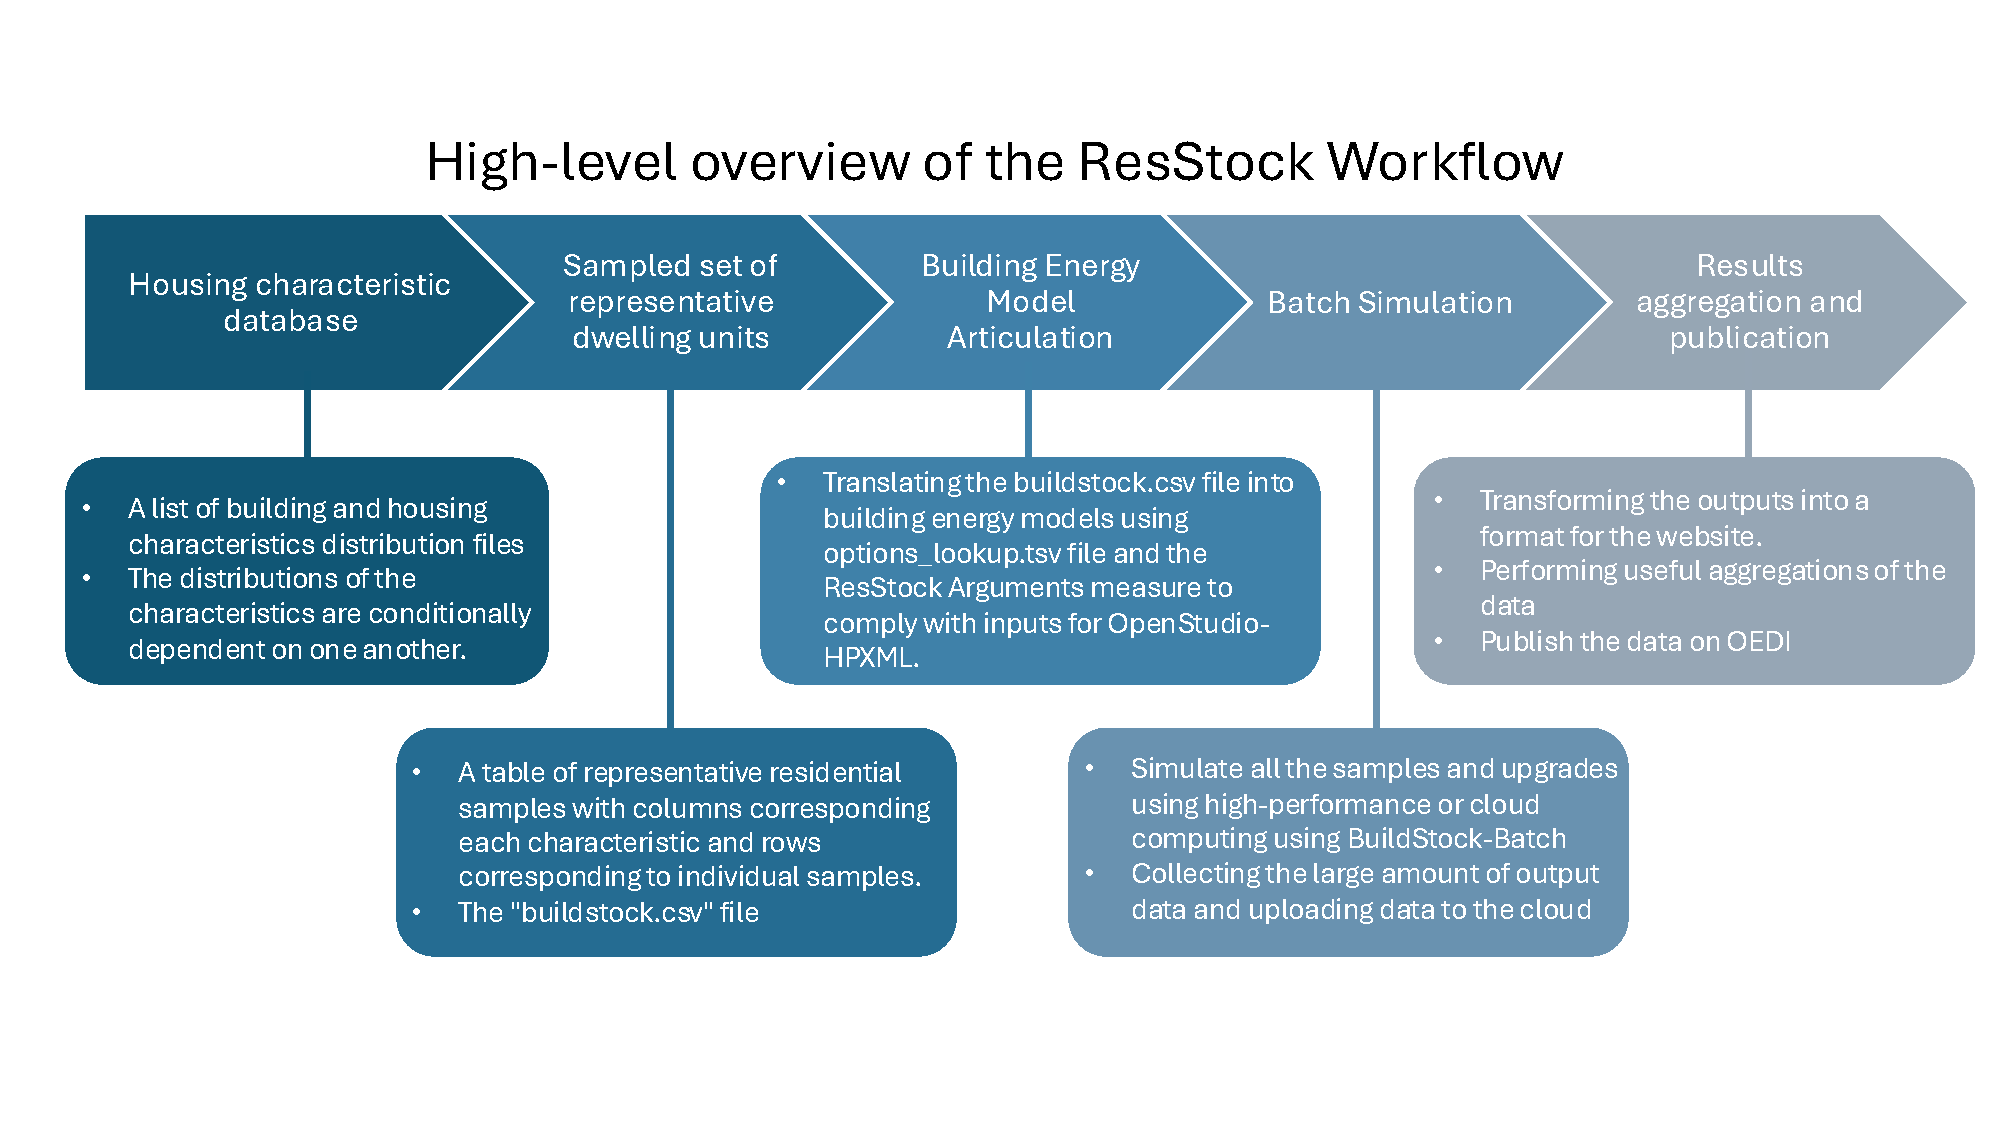
\includegraphics[width=1\linewidth]{images/ResStock-Workflow-Graphic-Simple.pdf}
    \caption{A high-level overview of the ResStock workflow steps and what occurs during those steps}
    \label{fig:workflow_overview}
\end{figure}

\section{Residential Building Stock Characterization}
ResStock characterizes the U.S.~residential building stock and the associated occupants using a probabilistic representation of building and household characteristics developed using the best available data. Much of the underlying data for the U.S.~residential stock comes from national survey data. These surveys include the \href{https://data.census.gov/}{U.S.~Census}, the \href{https://www.census.gov/programs-surveys/acs/microdata.html}{Public Use Microdata Sample} (a microdata version of the American Community Survey [ACS]), the \href{https://www.census.gov/programs-surveys/ahs.html}{American Housing Survey (AHS)}, and the EIA's \href{https://www.eia.gov/consumption/residential/}{Residential Energy Consumption Survey (RECS)}. These surveys provided weighted survey samples with different building characteristics (for example: heating fuel, vintage, number of occupants, floor area, etc.) that ResStock leverages.

ResStock takes this survey microdata, processes it, and connects it to other surveys to develop housing characteristic probability distributions. 

%An example result of this process is the Vintage characteristic distribution of the housing units in the United States. This distribution shows when residential housing units were built in the United States:
%\begin{itemize}
%    \item 13\% of residential housing units were constructed before 1940
%    \item 15\% were constructed between 1940--1959
%    \item 26\% were constructed between 1960--1979
%    \item 27\% were constructed between 1980--1999
%    \item 14\% were constructed between 2000--2009
%    \item 5\% were constructed since 2010
% \end{itemize}
 
%Within each vintage bin, we specify additional distributions of over 150 different characteristics in ResStock. 

Some of these characteristics include the location of the housing unit (examples: state, county, climate zone), the geometry of the housing unit (examples: building type, foundation type, floor area, number of floors), the envelope information (examples: wall insulation, attic type, window panes), appliances (examples: age of refrigerator, heating fuel of the cooking range, whether the unit has in-unit laundry), heating ventilating and air-conditioning (HVAC) system (examples: heating system type, cooling system type, setpoint temperatures, whether the housing unit has ducts), water heating (examples: water heating fuel, type of water heater), household information (examples: income, number of occupants, and tenure). ResStock only contains discrete distributions, and even continuous variables like vintage or floor area are discretized into bins. A given discrete bin of the distributions is referred to as an ``option'' of the characteristic. For example, in the Foundation Type characteristic, there is an option for the unit to have an ``unheated basement'' and another option for the unit to have a ``heated basement.'' Another example is that the Geometry Floor Area characteristic has an option for a housing unit to have a floor area between 1,000 and 14,999 ft\textsuperscript{2}.

%%%%Future improvement - add table of example ResStock characteristics

The input distributions also capture important correlations between building characteristics, sometimes referred to as conditional dependencies. For example, in Los Angeles, CA, in the 1960s, many residential buildings were constructed, while other cities may have seen growth at different periods. This is captured in ResStock by making the Vintage characteristic conditionally dependent on the location of the housing unit, so different locations will have different distributions of housing age. Another example is that energy codes became more widespread in the late 1970s, causing minimum insulation values in new homes to increase. This relationship is captured by making the Insulation characteristics, like wall insulation, conditionally dependent on vintage. Through these correlations taken from the survey data, a network of characteristics and conditional dependencies are assigned through ResStock characteristic variables. It is these conditional dependent distributions of the characteristics that create the residential building stock characterization in ResStock. Information about how these distributions are created can be found in Section \ref{hc_overview}. Detailed information about each characteristic, assumptions, dependencies, and data sources can be found in Section \ref{sec:resstock_inputs}.

ResStock does not model actual buildings (for example: the apartment complex at 123 Main Street). Instead, the housing characteristic distributions are sampled hundreds of thousands of times---typically 550,000---to create a synthetic stock representation of U.S.~housing units. Each sampled housing unit is assigned an option for each of the ResStock housing characteristics. Within the ResStock workflow the full set of sampled housing units and their associated characteristics is referred to as the \texttt{buildstock.csv}. An illustrative example of some characteristics of a ResStock model is shown in Figure \ref{fig:illustrative_sample}. More information about how the sampling is performed can be found in Section \ref{sec:sampling_methodology}. Each of the 550,000 representative samples in the \texttt{buildstock.csv} can be thought of as an archetype residential housing unit description, meaning that each synthetic building represents approximately 250 real U.S.~housing units.

\begin{figure}
    \centering
    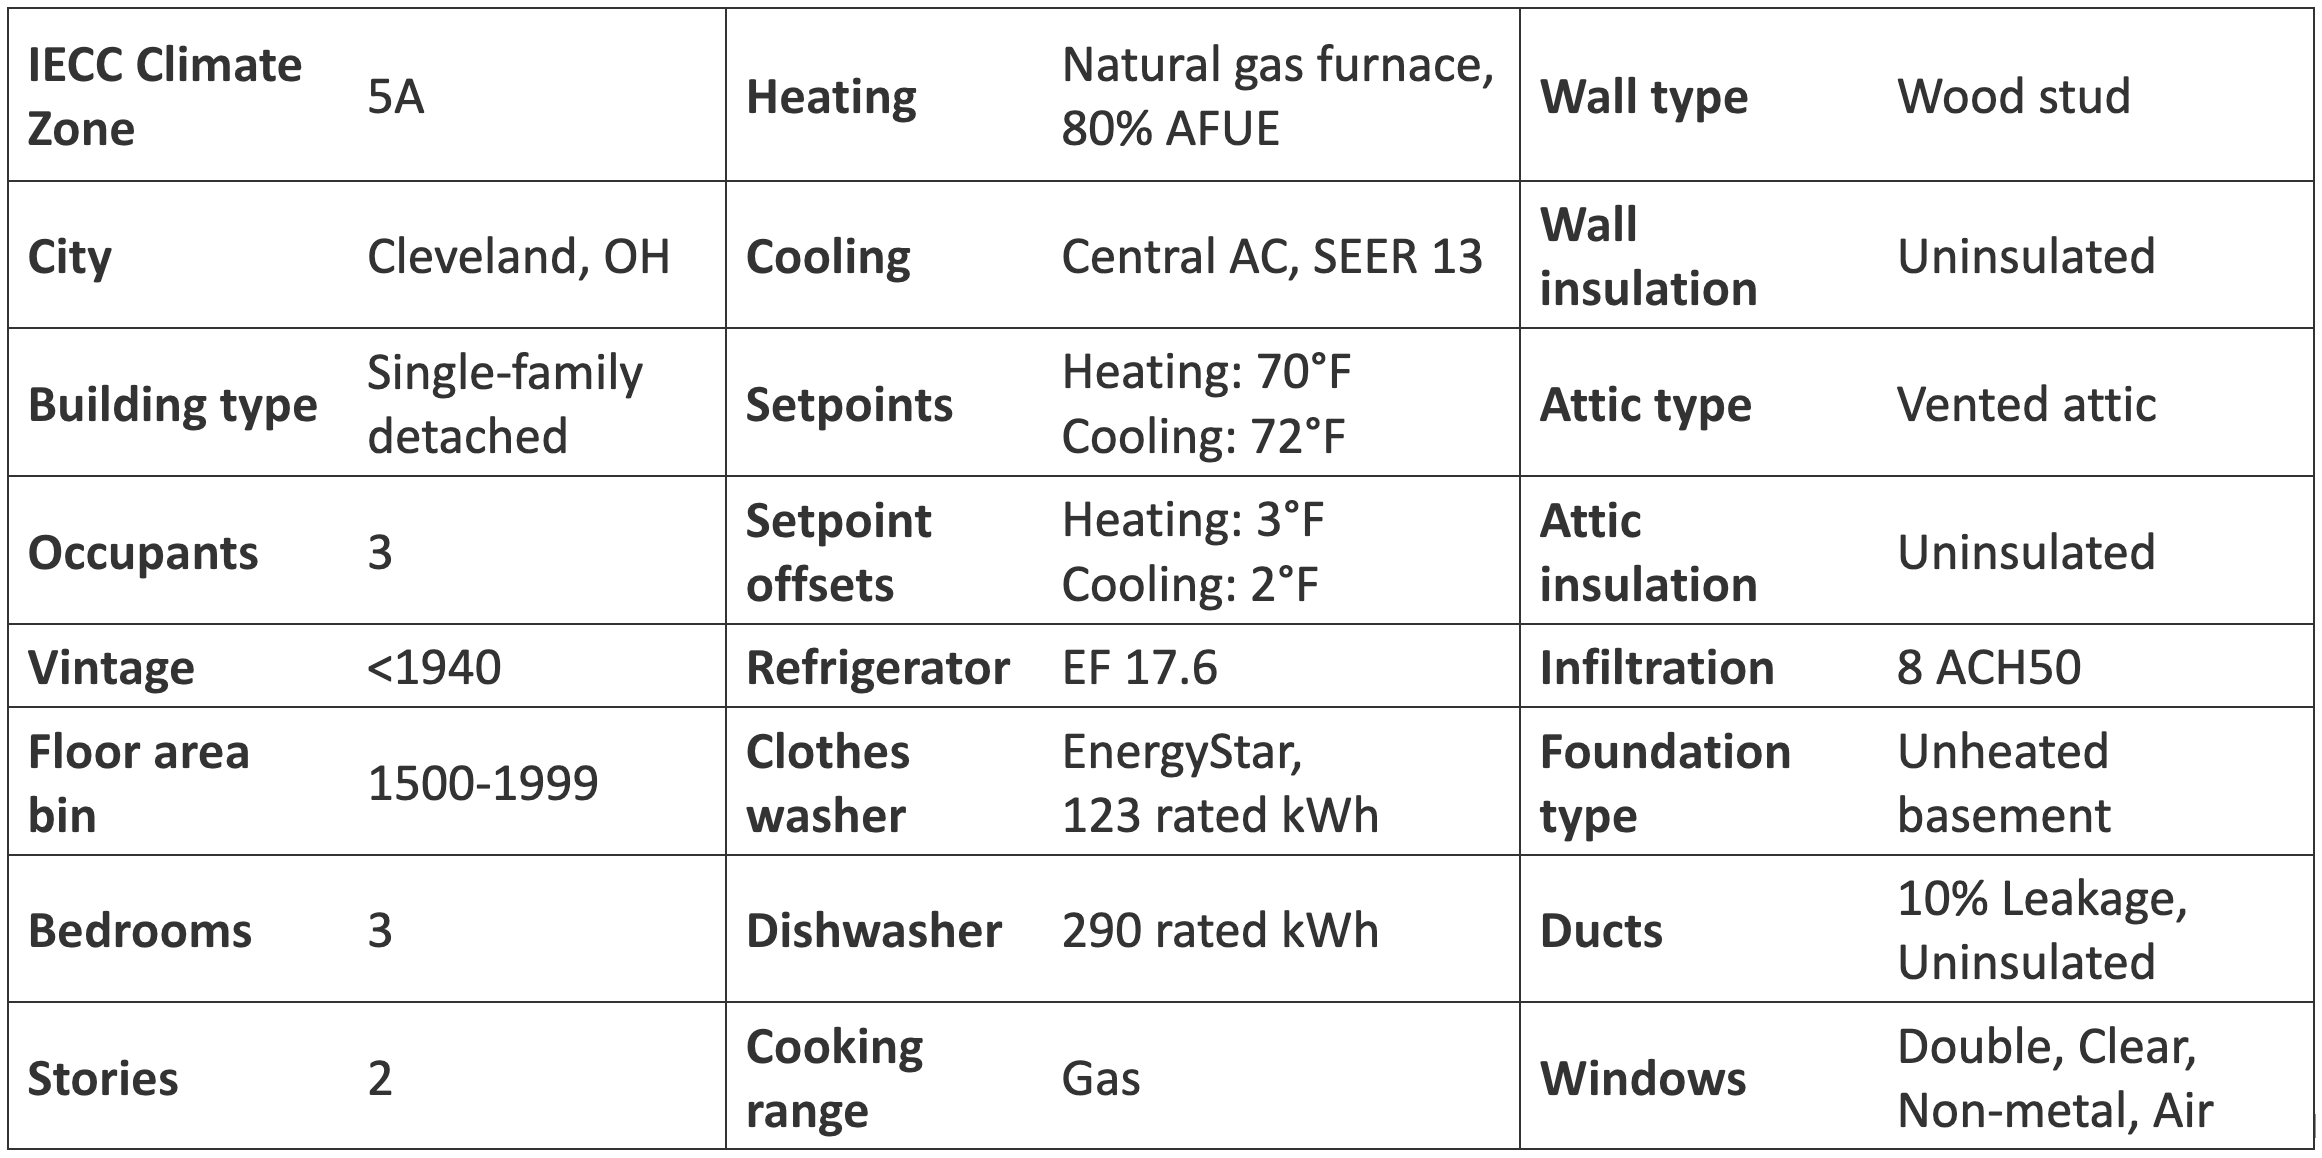
\includegraphics[width=1\linewidth]{images/illustrative_sample.png}
    \caption{An illustrative example of a representative housing unit sample from ResStock (does not show all characteristics available in ResStock)}
    \label{fig:illustrative_sample}
\end{figure}

\section{Building Energy Model Articulation} \label{sec:bem_articulation}
After sampling is complete, the \texttt{buildstock.csv} file contains the synthetic housing stock, with each row representing a sampled housing unit and each column containing a different ResStock housing characteristic. Each housing characteristic has an option assigned for each sampled housing unit in the synthetic stock. The table itself is a set of string values that need to be transformed into a building energy model for each sampled housing unit. The transformation of a single line of characteristic options, (see Figure \ref{fig:illustrative_sample} for an example) into an EnergyPlus building energy model is referred to as the model articulation process.

ResStock can be run either just for ``baseline'' energy use---i.e., energy use in the present-day housing stock---or with ``upgrades'' that will simulate both the baseline as well as a technical potential of different technologies to change energy use and associated metrics. The foundation of each of these workflows is the model articulation process. This document discusses primarily the ResStock baseline state since each public data release of upgrade measures has its own accompanying detailed technical documentation. 

% Option lookup, map options to arguments
The first step in the model articulation process maps the options for each housing characteristic within a single row of the \texttt{buildstock.csv} to ResStock modeling arguments. For reference, the mapping is specified in the \href{https://github.com/NREL/resstock/blob/v3.3.0/resources/options_lookup.tsv}{options\_lookup.tsv} file. This file contains all the housing characteristics and all the housing characteristic options in the ResStock national residential stock characterization and the associated ResStock model arguments. This file also includes housing characteristic options that are not sampled in the ResStock baseline, but which could be applied as upgrade options. A list and description of all the ResStock arguments can be found on the \href{https://github.com/NREL/resstock/tree/v3.3.0/measures/ResStockArguments}{ResStock GitHub Repository}. For ResStock to model any option, either in baseline or in upgrade, that option must exist as a \texttt{characteristic | option}  pair in the associated \textit{options\_lookup.tsv}. For example, if there exists a pair \textit{Windows|Double, Clear, Non-metal, Air}, that is then available for use in the baseline housing stock distributions and in upgrade specifications in the project specification file. A \texttt{characteristic | option} pair does not need to exist in the baseline to be used in an upgrade. The technical details associated with each option of the housing characteristics are defined in the \href{https://github.com/NREL/resstock/blob/v3.3.0/resources/options_lookup.tsv}{options\_lookup.tsv} file. For example, the wall exterior finish option: Wood, Medium/Dark is translated into a medium dark color wood siding with an exterior finish R-value of 1.4 in the ResStock measure, which is transformed into other model file inputs. While the ResStock housing characterization provides many inputs that ultimately make up a building model sample (see Section \ref{sec:bem_articulation} for model articulation), it’s important to recognize that there are far more technical details that are not characterized by ResStock, e.g., how much windows are being shaded, how much natural ventilation is used over the course of the year. Instead, these parameters assume the default values from OS-HPXML. For more details on modeling assumptions, refer to the \href{https://openstudio-hpxml.readthedocs.io/en/v1.8.1/}{OS-HPXML documentation} and Section \ref{sec:resstock_inputs} on how building systems are modeled.

Many housing characteristic options are directly used in the creation of the EnergyPlus models, but some are just structural in developing the probability distributions. For example, the ASHRAE IECC Climate Zone 2004 characteristics set the \texttt{site\_iecc\_zone} and \texttt{site\_type} ResStock arguments (Section \ref{sec:ashrae_2004_tsv}), but Location Region is just used as a dependency to define other characteristics that impact the energy modeling. Housing characteristics that do not assign an argument are called meta-parameters, for example Federal Poverty Level. These meta-parameters are often used as intermediate dependencies in other characteristics to separate key housing characteristics that influence the energy simulation. For example, the Federal Poverty Level characteristic and options are used to correlate income to appliance ownership and efficiency. The options and arguments for each ResStock housing characteristic are discussed in detail in Section \ref{sec:resstock_inputs}. 

\section{OpenStudio--HPXML}

% ResStock arguments to OpenStudio-HPXML arguments, the HPXML file, class abstraction of the HPXML schema, creation of HPXML file, and the translation of the OpenStudio model.
The next step in the workflow is converting ResStock arguments to the OpenStudio-HPXML arguments to create the HPXML file. OpenStudio-HPXML uses a series of OpenStudio measures to generate an EnergyPlus model for each sample based on the building and occupant characteristics defined by ResStock (Figure \ref{fig:os-hpxml}). In many cases, ResStock relies upon the OpenStudio-HPXML default arguments and calculations. The OpenStudio measures called in the workflow are:

\begin{itemize}
    \item \textbf{BuildExistingModel} -- meta-measure that calls on all following measures in the workflow and passes in ResStock files
    \item \textbf{ResStockArguments} -- translates housing characteristics from ResStock into arguments for BuildResidentialHPXML
    \item \textbf{BuildResidentialHPXML} -- creates the HPXML file for ResStock sample and calculates defaults if not provided from ResStock
    \item \textbf{BuildResidentialScheduleFile} -- generates schedules and references the \texttt{schedules.csv} from the HPXML file
    \item \textbf{ApplyUpgrade} -- meta-measure that calls the following measures in the workflow to modify arguments for samples that have upgrade scenarios applied. 
    \item \textbf{HPXMLtoOpenStudio} -- translation of the HPXML file to an OpenStudio model.
\end{itemize}

\begin{figure}
    \centering
    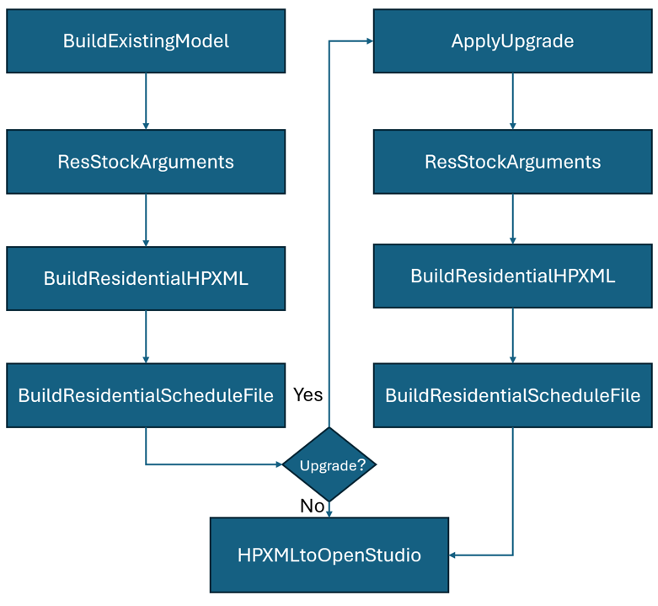
\includegraphics[width=1\linewidth]{images/OSHPXML.png}
    \caption{Flowchart of OpenStudio measures performed to translate a ResStock sample into an OpenStudio model}
    \label{fig:os-hpxml}
\end{figure}

Throughout this translation process, in most cases, the ResStock arguments are the same as the final OpenStudio-HPXML arguments assigned in BuildResidentialHPXML. An example of an identical argument is \texttt{geometry\_unit\_num\_bedrooms}. However, there are some instances where the ResStock arguments intentionally differ from the OpenStudio-HPXML arguments and need further adjustment.  Another potential difference is combining and modifying ResStock arguments into one OpenStudio-HPXML argument. An example is using \texttt{air\_leakage\_percent\_reduction} as part of an envelope upgrade that reduces infiltration. In this scenario, the \texttt{air\_leakage\_value} is adjusted by the \texttt{air\_leakage\_percent\_reduction} argument.

\section{Batch Simulation}
% BuildStock-Batch for the sampling, batch simulation, and post-processing
% Introduce that some parallelization is needed. The computations can either be done on the a local machine, a high-performance computing machine, or even the cloud. A lot of data is produced, post-processing is the biggest memory process.
% The different jobs (sampling/job setup, the array job, and post-processing).
The model articulation process discussed in the previous sections is performed for each of the 550,000 ResStock samples; when factoring in upgrade scenarios, this can result in tens of millions of EnergyPlus simulations. The NREL-developed software \href{https://github.com/NREL/buildstockbatch/tree/v2023.10.0}{BuildStock Batch} manages the various stages of the workflow of running ResStock or ComStock. BuildStock Batch has its own \href{https://buildstockbatch.readthedocs.io/en/v2023.10.0/index.html}{documentation} for a detailed understanding of the software. BuildStock Batch can be run locally, on NREL's high-performance computing (HPC) system, or on the cloud using Amazon Web Services (AWS) or Google Cloud Platform. The local version of BuildStock Batch is mainly used for testing purposes during new feature development and for use in the continuous integration of the ResStock and ComStock software stack. The local version is not used for production-scale runs due to the typically low number of CPU cores and limited memory of local machines. The HPC- or cloud-based workflows can be used to run the full set of baseline samples and upgrade simulations, but all public runs up through 2024 have been completed on NREL's HPC system.

BuildStock Batch is initialized with a project file that configures all the inputs to the workflow. An \href{https://github.com/NREL/resstock/blob/develop/project_national/national_baseline.yml}{example project file} to simulate the national baseline stock can be found in the ResStock repository. There are three major steps to the BuildStock Batch workflow: (1) sample creation and job setup, (2) parallel simulation of all baseline and upgrade simulations, and (3) collection of output data from the simulations and upload to AWS for querying. The sampling and job setup process creates the sampled description of the housing characteristics in the ``buildstock.csv'' file. Then BuildStock Batch submits a job that runs all the simulations in parallel by performing the model articulation and the EnergyPlus simulation for each sample. To run these simulations efficiently, BuildStock Batch communicates with the computing nodes to manage the computing resources at every stage of the workflow. In particular, the software facilitates the simulations in batches by breaking them up into smaller jobs that can be run by parallel processors or by multiple nodes in a distributed manner. This is critical for enabling large-scale simulations which are often time- and memory-intensive to process. BuildStock Batch makes it possible to run hundreds of thousands of simulations in a timely manner by leveraging HPC. After the simulation completes for each model, the workflow post-processes the simulation output by compiling them into annual summary files and coalescing the timeseries into partitioned files separated by upgrade scenario and other user-specified characteristics such as state and county. As the final step, BuildStock Batch can optionally upload the result files to AWS S3 storage, where they can be queried much like a database using web services such as AWS Athena.

A successful run of 550,000 samples with no upgrades, a 15-minute time step, no errors, and no queue time can typically be run on NREL's HPC system within a few hours and creates about 500 GB of output. 

\section{Upgrade Specification}\label{sec:upgrades}
In ResStock, most of the details of upgrade specification occur directly in the project file under the \href{https://buildstockbatch.readthedocs.io/en/v2023.10.0/project_defn.html#upgrade-scenarios}{upgrades key}, using fields from the \texttt{options\_lookup.tsv} file specified in logic blocks. Options specified for upgrades include which segment of the baseline the upgrade should be applied to, cost multipliers, and the ``reference'' case, which is important if doing a comparison against a business-as-usual scenario (especially for costs). If the upgrades section is not specified, only the building stock baseline will be simulated. Details of the upgrades associated with each ResStock data release can be found in the supporting upgrade measure documentation.

ResStock upgrades are deterministic, not probabilistic, similar to how the baseline is constructed. You can specify, for example, that all housing units with a specific existing air conditioner in baseline get a specific new air conditioner in upgrade. Or you can use more complex logic and specify 10 different air conditioners in upgrade, based on any characteristic or combination of characteristics. But each housing unit will deterministically receive a specific new air conditioner based on the logic. This can cause challenges. One example is if specifying a new air conditioner for housing units that don't already have air conditioning, you might ideally specify a new, probabilistic range of cooling setpoints for those homes. However, this is not possible. This is why ResStock specifies cooling setpoints for every housing unit, whether or not the unit has air conditioning: so that if an upgrade run assigns air conditioning to that housing unit, the resulting setpoints are appropriately diverse. One can think of this situation as the housing unit's preference of a cooling setpoint if one had a cooling system. There are several other similar parameter option specifications in baseline that are not used to model the baseline but are available in case of certain upgrade option assignments. 

%%%% postprocessing

%%%Need to talk about failed simulations, how they get removed from SDR, and potential implications in representative count (why we say 550k but it's always less than that). How postprocessing sometimes also has to remove buildings with upgrades but no baseline.

\section{Results and Publication}
The results from the BuildStock Batch post-processing include: (1) metadata and annual results (referred to as the \texttt{results.csv} file), (2) a set of end-use timeseries parquet files that combine all the end-use timeseries results from the 550,000 models, and (3) a compressed set of building simulation folders with the results of the OpenStudio-HPXML workflow for each building sample. The \texttt{results.csv} file includes the housing characteristics and annual energy, emissions, utility bills, and cost multipliers for each of the 550,000 models. When a production run of ResStock is completed, reviewed, and ready for publication, the outputs are then reformatted so that each building timeseries is a single file, the result columns start with ``in.<input>'' and ``out.<output>'' (instead of ``build\_existing\_model'' and ``simulation\_output\_report,'' the original outputs of OpenStudio-HPXML), and the energy results are all converted to kWh. This extra step is done in part for readability and ease of use, and also because the \href{https://resstock.nrel.gov/datasets}{ResStock dataset viewer} allows all the energy outputs to be stacked on top of one another and expects the new naming convention. This step is also done outside of the BuildStock Batch workflow. After the conversion, the datasets are uploaded to the \href{https://data.openei.org/submissions/4520}{Open Energy Dataset Initiative End-Use Load Profiles} submission.

\chapter{Input Structure and Sampling} \label{sec:input_structure_and_sampling}
In this section, we discuss the structure of ResStock's input data and our sampling approach. This includes an overview of the probability theory behind ResStock's inputs, how we merge data sources, and how stochastic occupant schedules are created.


\section{Overview of Housing Characteristics} \label{hc_overview}
ResStock uses a set of conditional distributions to describe the characteristics of U.S.~housing units and the households living in them. There are over \href{https://github.com/NREL/resstock/tree/v3.3.0/project_national/housing_characteristics}{150 characteristics described in ResStock}, the majority of which describe the physical attributes of the buildings. Some demographic household characteristics are also included as inputs, both to describe the demographics of the households (e.g., income and renter/owner status) as well as to differentiate key appliance ownership and building characteristic differences that exist between households of different demographics. Each sample in ResStock represents one housing unit (as opposed to a building with many housing units) and will have a value selected for every input housing characteristic defined in ResStock. 

Table \ref{tab:ex_whf_distr} is an illustrative example of a conditional distribution table for the housing characteristic Water Heating Fuel. There are three parts to this table---options, dependencies, and sampling probability. The options are the values a characteristic parameter can take on (e.g., water heater fuel has the options: electricity, fuel oil, natural gas, other fuel, and propane). If one characteristic is described based on another, this is known as a dependency. The dependencies explain how the characteristic is distributed (e.g., Water Heater Fuel saturation varies based on Geometry Building Type RECS, Heating Fuel, and State). Since all buildings must receive a value assigned for a Water Heating Fuel option during sampling, the probabilities in the option columns are equal to one when summed row-wise. Each row gives the parameter distribution within a housing segment defined by the dependencies. For example, the Water Heating Fuel for Mobile Homes with a Heating Fuel of Electricity located in CA has a 72.37\% probability of being Electricity, and a 17.59\% probability of being Natural Gas.  The \textit{sampling\_probability} column provides the likelihood of sampling a home with the dependency characteristics, i.e., the relative size of the housing segment in the United States. The column can be extended with the option probability (i.e., each value under the option column) to give the joint probability of sampling the characteristics of both the dependencies and the option. For example, Mobile Homes with a Heating Fuel of Electricity located in CA represent 0.09022\% of the national residential housing units. Multiplying this by the 72.37\% probability of these housing units having Electricity as their Water Heating Fuel, we determine that Mobile Homes with a Heating Fuel of Electricity located in CA and having a Water Heating Fuel of Electricity represent 0.06529\% of the national residential housing stock.

\begin{table}
    \centering
    \scriptsize
    \begin{tabular}{p{0.2\linewidth}p{0.08\linewidth}p{0.075\linewidth}|
p{0.05\linewidth}p{0.05\linewidth}p{0.05\linewidth}p{0.05\linewidth}p{0.05\linewidth}p{0.075\linewidth}}
    \hline
    Dependency=Geometry Building Type RECS & Dependency=\newline Heating Fuel & Dependency=\newline State & Option=\newline Electricity  & Option=\newline Fuel Oil & Option=\newline Natural Gas & Option=\newline Other Fuel & Option=\newline Propane & sampling\newline \_probability \\
    \hline
    Mobile Home & Electricity & CA & 0.7237 & 0 & 0.1759 & 0 & 0.1005 & 0.0009022 \\
    Multifamily with 2--4 Units & Electricity & CA & 0.6379 & 0 & 0.3621 & 0 & 0 & 0.0026521 \\
    Multifamily with 5+ Units & Electricity & CA & 0.5690 & 0 & 0.4217 & 0 & 0.0093 & 0.0113951 \\
    Single-Family Attached & Electricity & CA & 0.6986 & 0 & 0.2696 & 0 & 0.0318 & 0.0019855 \\
    Single-Family Detached & Electricity & CA & 0.3200 & 0 & 0.6428 & 0 & 0.0372 & 0.0107185 \\
    \hline
    \end{tabular}
    \caption{Subset of Water Heating Fuel distribution}
    \label{tab:ex_whf_distr}
\end{table}

%To illustrate, let’s interpret the last row of Table \ref{tab:ex_whf_distr}. The sampling\_probability tells us that 1.07\% US housing units are single-family detached homes heated using electricity in California. This also means roughly one in 100 models sampled by ResStock will be in this housing segment. The five option columns (starting with Option=) show the probability distribution of water heating in this segment. The probability distribution for Single-Family Detached homes with electric space heating in California has 32.0\% of homes using Electricity for water heating, 0\% Fuel Oil, 64.28\% Natural Gas, 0\% Other Fuels, and 3.72\% Propane. Each of these option probabilities can be multiplied by the sampling\_probability to find the overall likelihood of that option being selected in ResStock. This is known as the joint probability. For example, the joint probability of selecting a Single-Family Detached home with electric space heating in California AND electric water heating is 0.3200 * 0.6528 = 0.34= 0.34\%. This can also be stated that 0.34\% of housing units in ResStock are in California, in Single Family Homes, with electric space heating and electric water heating.

%These dependencies of one housing characteristic on another form a directed acyclic graph in ResStock called the dependency graph. For example, the dependency graph for Bedrooms is shown in Figure \ref{fig:bedrooms_dependency_tree}. The Bedrooms housing characteristic defines the number of bedrooms in the housing unit. On the left side we can see the upstream dependencies of the Bedroom housing characteristic, which are all the characteristics that influence either directly (via a direct dependency) or indirectly (via dependencies further upstream on other nodes) the distribution of the Bedrooms housing characteristic. On the right side, we can see the downstream housing characteristics influenced by the Bedrooms housing characteristic. The color of the nodes indicate the source dataset used to characterize the different nodes in the network (i.e., the data source of the various housing characteristics). In this case, the green nodes come from the PUMS data, which is the microdata version of the American Community Survey, and the black nodes come from the American Housing Survey.  These dependency trees can be interactively generated and analyzed using the \href{https://github.com/NREL/resstock-estimation/blob/develop/utils/dependency_visualizer.py}{dependency\_visualizer} tool in the resstock-estimation repository.
%\begin{figure}
%    \centering
%    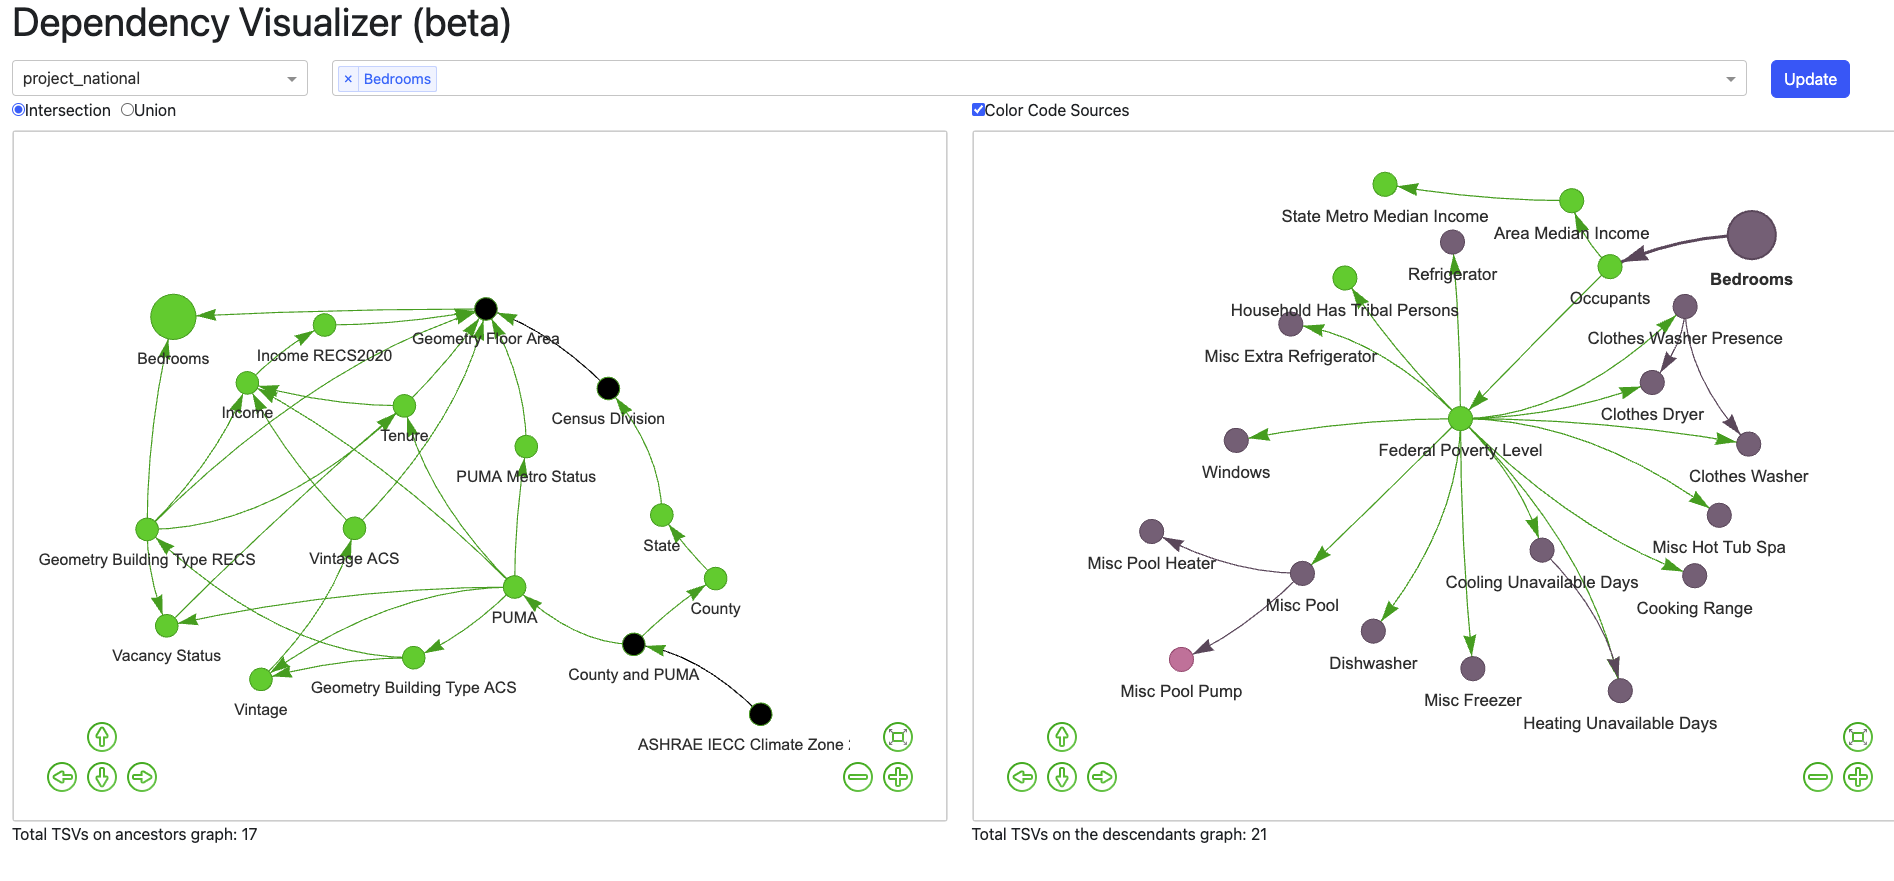
\includegraphics[width=0.9\linewidth]{ResStock Technical Reference Guide/images/bedroom_dependency_tree.png}
%    \caption{Example dependency tree for Bedrooms}
%    \label{fig:bedrooms_dependency_tree}
%\end{figure}

\section{Methods for Creating Housing Characteristic Distributions}\label{hc_method}
ResStock housing characteristics are mostly compiled using publicly available survey data. Major data sources include the Residential Energy Consumption Surveys (RECS) from the EIA \citep{RECS2020}, the Public Use Microdata Samples (PUMS) of the American Community Survey \citep{PUMS}, and the American Housing Survey \citep{AHS}. For certain characteristics that are not yet surveyed nationally, region-specific datasets are used instead. For example, the hot water fixture distribution is informed by field data from a demand management program in the Northeast. Roof insulation, ceiling insulation, and window area characterization come from the Residential Building Stock Assessments by the Northwest Energy Efficiency Alliance \citep{RBSA}. Some housing characteristic distributions are created manually as they do not have any survey data to base on, with about a quarter of ResStock's housing characteristics being constructed using reference numbers from studies. For example, the insulation level for ceilings and walls are derived from the Home Innovation Research Labs 1982--2007 data, and spot ventilation for bathroom and range hood comes from the Building America House Simulation Protocols (\cite{Wilson2014}). Ten characteristics are created based on engineering judgment, including things like door area, plug load diversity, and mechanical ventilation. Each input housing characteristic to ResStock is discussed in detail in Section \ref{sec:resstock_inputs}, including data sources and assumptions. 

ResStock updates housing characteristic distributions to the latest release of longitudinal surveys whenever possible and incorporates new data sources when a need and a data source are both identified. The housing characteristics captured in \href{https://resstock.readthedocs.io/en/v3.3.0/}{ResStock release v.3.3.0} represent the existing U.S.~housing stock as of approximately 2019 (housing stock: {\raise.17ex\hbox{$\scriptstyle\sim$}}2019, weather: 2018 or TMY3, and appliances: {\raise.17ex\hbox{$\scriptstyle\sim$}}2020). ResStock models the continental United States plus Alaska, although the latest data release includes only the continental United States. Hawaii is being added in 2025, and the next data release of ResStock will include all 50 states and the District of Columbia. ResStock does not currently model U.S.~territories such as Puerto Rico.

To generate a housing characteristic's distribution, we generate distributions as normalized cross tabulations of the variables and their dependencies using the sample weight in the source data. We select dependencies from the available variables in the surveys based on a combination of engineering judgment, empirical evidence of correlation, and the need to balance between data fidelity and variability. For example, we know there is likely to be a relationship between having natural gas as a space heating fuel and having natural gas as a water heating fuel since there is already natural gas service to the home, so we set Heating Fuel as a dependency for Water Heating Fuel. Engineering judgment can help pre-select a set of variables to correlate with the parameter. Then, the correlation is verified with empirical evidence that may include correlation matrices, statistical tests, and plots or tabulations demonstrating the significance of dependency variables to the output distributions. Input characteristics are constantly being evaluated and updated as better data are identified.

To ensure data fidelity and representativeness, each row in a distribution is generally informed by at least 10 samples in the source data. The number of dependencies to include is limited by the size of the source data, since the data will be sliced over many parameters to generate each row of the distribution. For example, smaller source datasets can afford splitting over fewer or less granular dependencies before the data is spread too thin. In such cases, it becomes necessary to choose variables that best capture the variability in the parameter. To do this, we use graph theory and Bayesian inference to calculate the incremental information gain by each candidate variable, which ranks them for selection. Sometimes the dependency selection is further limited to keep the distribution to a manageable file size for workflow purposes. For example, a distribution with a dependency on County will likely have few other dependencies, as doing so will result in an oversized distribution that cannot be stored in the GitHub repository and is otherwise difficult to work with since there are over 3,100 counties in the United States.

In addition to strategic dependency selection, ResStock has two other approaches for dealing with low samples or missing dimensionality in the source data: fallback rules for dimensional coarsening and dimensional blending. Some characteristics in ResStock have several granularity options available, e.g., Vintage (housing unit age grouped into 10 bins) vs.~Vintage ACS (housing unit age grouped into 6 bins). These granularity options help bridge between source data that have different native resolutions to connect the derived distributions. They are also used in fallback rules and dimensional coarsening to address low samples. A common practice in ResStock is to fill the cross tabulation using the native resolution of the dependency variables. Then where there’s insufficient sample count, ResStock pulls the distribution from higher granularity variables to fill the rows. For example, state-level tabulation can be used to fill or supplement the rows with low samples that are natively at the county level. This dimensional coarsening may result in some rows sharing similar probability distributions but at the benefit of filled data gaps and higher sample confidence. The fallback rules are what define these processing sequences so that some or all dependency variables can be coarsened incrementally until all rows reach enough samples. Dimensional coarsening is commonly done over geography, climate zone, vintage, building type, floor area, and income by grouping together similar options or options believed to influence energy consumption similarly (e.g., neighboring geographies). In Section \ref{sec:resstock_inputs} we discuss in the assumptions section for each variable if dimensional coarsening is used.

Another approach to dealing with low samples or missing dimensionality is dimensional blending. This simply refers to updating one distribution with another distribution, hence “blending” the two distributions together. Dimensional blending is often used when a distribution lacks the desired granularity natively and is therefore augmented by another distribution with that granularity. For example, the windows distribution in ResStock comes from RECS, which characterizes the windows based on glass type and frame material. To augment the window options to account for storm window and low-e glazing, the distribution is re-normalized using proportionalities derived from shipment data.

The full cross-tabulation of a parameter and its dependencies can sometimes give rise to impossible or highly improbable combinations of characteristics, e.g., single-family houses that are over 8 stories tall. These combinations are assigned a parameter value of “void,” and prune rules are used in the distribution development to ensure that such combination will never be sampled. If such combination is accidentally sampled (perhaps due to error in upstream housing characteristics), then this will be caught immediately since ``voids'' are supposed to be un-sample-able. Some characteristic combinations are realistic but may be pruned due to limitations in the upstream modeling workflow. For example, in ResStock, single-family detached houses that are 0--1,499 ft\textsuperscript{2} with attached garages can currently only have a single-car garage. This is due to ResStock assuming a specific aspect ratio for building footprint and modeling constraints restricting that the garage cannot be larger or deeper than the livable space.

Many of the housing characteristic distributions are validated by comparing their marginal distribution by each dependency with those of the source data. This is to ensure that any special handling of the data to address low samples or missing dimensionality do not deviate the distributions significantly from the source data. The parity maintained with the source data also means the housing characterization in ResStock inherits the same level of survey biases or uncertainty as those that exist in the source datasets. For example, ResStock’s characterization of Mobile Homes has higher uncertainty than any other housing types as mobile homes are the least common of the major housing types (single-family, multifamily 2--4 units, etc.), and fewer data points exist for them in the source datasets. While using the survey sample weight to construct the distributions helps ensure they are representative of the U.S.~housing stock, ResStock does compare the effect of using different types of sample weight when they are available in certain surveys, such as RECS.



\section{Sampling Methodology} \label{sec:sampling_methodology}
 With the full conditional probability network of inputs defined, ResStock samples the inputs to create the synthetic housing stock. The input file structure and dependency network determines the order in which each characteristic is sampled. Sampling starts with housing features that have no dependencies and next moves to characteristics that have dependencies on the first level of characteristics sampled. This process proceeds until all inputs are sampled and defined. For example, Figure \ref{fig:ex_build_char_distrs} shows an example set of housing characteristic distributions that are interconnected by dependencies. To create a building model in this hypothetical network, the census division is sampled first (and Middle Atlantic is chosen). Then the vintage of the model is sampled based on the distribution of vintage for the chosen census division (1980s is chosen). Next, the heating fuel is sampled according to the distribution for the chosen vintage (natural gas is chosen), and this process repeats until all housing characteristics are determined.  

\begin{figure}
    \centering
    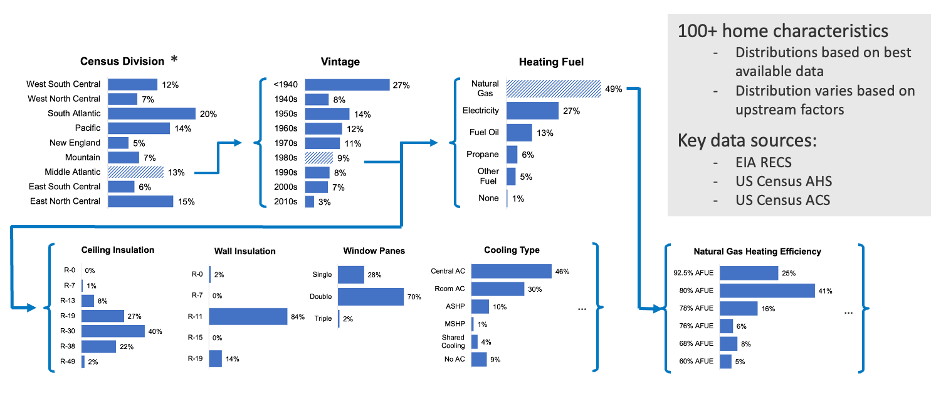
\includegraphics[width=1\linewidth]{images/cond_prob.png}
    \caption{Example of interconnected building characteristic distributions}
    \label{fig:ex_build_char_distrs}
\end{figure}

To create a full representative synthetic housing stock for the United States, ResStock employs quota-based sampling. In quota-based sampling, building models are created until the specified number of samples (i.e., the quota) is reached. Sampling starts with the most likely characteristics or most common housing unit in the United States, and then continues filling out increasingly less-likely combinations of characteristics until the quota is reached. This approach creates building models with equal sample weight, meaning each sampled housing unit represents the same number of housing units in the real housing stock. This is a product of quota-based sampling where the likelihood of a building characteristic is directly reflected in the number of times that characteristic is sampled instead of being included in the sample weight.

The quota-based sampling approach is different from purely random sampling (e.g., Monte Carlo) where the samples can come from anywhere in the distributions. Random samples thus may not be representative until many samples are drawn. In quota-based sampling, the quota is multiplied by the probability distributions to determine how many samples will have certain characteristics. If natural gas accounts for 50\% of space heating in the marginal distribution, then one in two samples will be decidedly heated by gas, and this holds true for a quota of two or a quota of a million. However, larger quotas are required to sample uncommon characteristics due to the discretization effect (i.e., a characteristic of 0.1\% probability will not show up in a sampling quota of 500 as 0.1\%*500 = 0.5, which is less than one sample). It's worth noting that the characteristics doesn't need to be uncommon at the national scale for this problem to occur. Even if a characteristic has 1\% probability nationwide, we will not get the expected 0.01 * 550,000 = 5,500 samples in a national run and in fact may get zero samples if the characteristic has dependencies that will cause it to be sampled within thousands of slices of (quota of) less than 100 samples. While such extreme cases are uncommon, most characteristics do have biases on their national-scale saturation over what one would expect based on the housing characteristic distribution due to this quirk of quota sampling. 

While the diversity in the samples scales with quota in both sampling methods, the rate of reaching a reasonable diversity or converging to the population mean is much faster for quota-based sampling than random sampling. The convergence rate is proportional to the square-root of the quota for quota-based and to the quota for random sampling. The ability to sample for characteristics proportional to their distributions makes quota-based sampling effective as the representativeness of the sampled stock is better maintained even at smaller sampling quotas.

For public datasets, different versions of ResStock runs will by default have different samples. Building model ID 1 is not the same between published datasets.

\section{Schedule Creation}\label{occupancy_model}
In addition to the housing characteristic input files, occupant and energy use schedules are another major necessary building energy model input. Most ResStock schedules are also based upon survey data, but we use a different approach for generating these schedule files since they need to be temporally comprehensive (typically covering a full year with 15-minute time steps) as well as sufficiently diverse to appropriately represent the range of load shapes that occur within the housing stock as well as the aggregate total.

\begin{table}
    \centering
    \scriptsize
    \begin{tabular}{l|l|l|l}
    \hline
    Schedule Name & Unit & Description & Stochastic? \\
    \hline
    \texttt{occupants} & frac & Occupant heat gain schedule & Stochastic \\
    \texttt{lighting\_interior} & frac & Interior lighting energy use schedule & Stochastic \\
    \texttt{lighting\_exterior} & frac & Exterior lighting energy use schedule & Non-Stochastic \\ 
    \texttt{lighting\_garage} & frac & Garage lighting energy use schedule & Stochastic \\
    % \texttt{lighting\_exterior\_holiday} & frac & Exterior holiday lighting energy use schedule. & Non-Stochastic \\
    \texttt{cooking\_range} & frac & Cooking range \& oven energy use schedule & Stochastic \\
    \texttt{refrigerator} & frac & Primary refrigerator energy use schedule & Non-Stochastic \\
    \texttt{extra\_refrigerator} & frac & Non-primary refrigerator energy use schedule & Non-Stochastic \\
    \texttt{freezer} & frac & Freezer energy use schedule & Non-Stochastic \\
    \texttt{dishwasher} & frac & Dishwasher energy use schedule & Stochastic \\
    \texttt{clothes\_washer} & frac & Clothes washer energy use schedule & Stochastic \\
    \texttt{clothes\_dryer} & frac & Clothes dryer energy use schedule & Stochastic \\
    \texttt{ceiling\_fan} & frac & Ceiling fan energy use schedule & Stochastic \\
    \texttt{plug\_loads\_other} & frac & Other plug load energy use schedule & Stochastic \\
    \texttt{plug\_loads\_tv} & frac & Television plug load energy use schedule & Stochastic \\
    %\texttt{plug\_loads\_vehicle} & frac & Electric vehicle plug load energy use schedule. & No \\
    \texttt{plug\_loads\_well\_pump} & frac & Well pump plug load energy use schedule & Non-Stochastic \\
    \texttt{fuel\_loads\_grill} & frac & Grill fuel load energy use schedule & Non-Stochastic \\
    \texttt{fuel\_loads\_lighting} & frac & Lighting fuel load energy use schedule & Non-Stochastic \\
    \texttt{fuel\_loads\_fireplace} & frac & Fireplace fuel load energy use schedule & Non-Stochastic \\
    \texttt{pool\_pump} & frac & Pool pump energy use schedule & Non-Stochastic \\
    \texttt{pool\_heater} & frac & Pool heater energy use schedule & Non-Stochastic \\
    \texttt{hot\_tub\_pump} & frac & Hot tub pump energy use schedule & Non-Stochastic \\
    \texttt{hot\_tub\_heater} & frac & Hot tub heater energy use schedule & Non-Stochastic \\
    \texttt{hot\_water\_dishwasher} & frac & Dishwasher hot water use schedule & Stochastic \\
    \texttt{hot\_water\_clothes\_washer} & frac & Clothes washer hot water use schedule & Stochastic \\ \texttt{hot\_water\_fixtures} & frac & Fixtures (sinks, showers, baths) hot water use schedule & Stochastic \\
    \texttt{heating\_setpoint} & $\deg$ F & Thermostat heating setpoint schedule & Non-Stochastic \\
    \texttt{cooling\_setpoint} & $\deg$ F & Thermostat cooling setpoint schedule & Non-Stochastic \\
    \texttt{water\_heater\_setpoint} & $\deg$ F & Water heater setpoint schedule & Non-Stochastic \\
    \texttt{water\_heater\_operating\_mode} & 0/1 & Heat pump water heater operating mode schedule. 0=hybrid/auto, 1=heat pump only. & Non-Stochastic \\
    % \texttt{battery} & frac & Battery schedule. Positive for charging, negative for discharging. & Non-Stochastic \\
    \texttt{vacancy} & 0/1 & Vacancy schedule. 0=occupied, 1=vacant. Automatically overrides other columns. & Non-Stochastic \\
    %\texttt{outage} & 0/1 & Power outage schedule. 0=power. 1=no power. Automatically overrides other columns. & N/A \\
    \hline
    \end{tabular}
    \caption{Modeled schedules in ResStock}
    \label{tab:schedules}
\end{table}


In ResStock, schedules are used to define a variety of building system operations (Table \ref{tab:schedules}). For example, the space heating and cooling system maintains the indoor air temperature according to a detailed schedule of heating and cooling setpoint temperatures. Interior lighting turns on according to occupancy, while exterior lighting is set to turn on at a specific time frame between the evening and the early morning. These schedules represent either preset equipment schedules, typical usage patterns, or the stochastic time use behaviors of all occupants living within a household. Occupant-driven schedules are typically heterogeneous to represent a diversity of behaviors and preferences. Many of the schedules capture not only the timing of use but also the intensity of use as fractional values, with diversity for every day of the year. These fractional value timeseries are then multiplied by the annual end-use energy or hot water use (calculated separately according to building simulation standards such as ANSI/RESNET/ICC 301 standard or those developed by \cite{bahsp_2010}, \cite{bahsp_2014}) to generate the respective end-use load profiles or hot water draw profiles. The schedules are modified for vacant units and vacancy periods (i.e., an occupied household goes on vacation). When a unit is unoccupied for either reason, all schedules are set to zero except for HVAC setpoint temperature schedules designed to keep pipes from freezing. See Section \ref{vacant_units} for more information. In ResStock, schedules are generated either using a stochastic occupancy generator (inherited from OS-HPXML) or through more simplistic defined schedules. %For power outage simulations, all schedules are set to zero except occupancy and general water draws during the periods of the outage. ResStock sets the outage periods via options\_lookup.

\textbf{Stochastic Schedules}. ResStock uses a stochastic schedule generator to produce representative and heterogeneous schedules for occupancy and a number of appliances and hot water end uses. Developed using the \href{https://www.bls.gov/tus/}{American Time Use Survey (ATUS) data from 2013--2017}, submetered appliance energy data, and a supplemental hot water model, the generator combines Markov chain and probability-sampling for schedule simulation. At a high level, the generator uses Markov chain models built from the ATUS data to produce occupant activity schedules for seven different activities: sleeping, personal hygiene, laundry, cooking, dish washing, absent, and active-at-home. These schedules are then processed and combined with appliance information to form household-level appliance and hot water schedules. For example, both clothes washer and clothes dryer events are scheduled to occur during laundry activity, whereas sink events are scheduled to occur during active-at-home activity. More details of the stochastic occupant model can be found in \citet{Chen2022}.

One of the housing characteristics in ResStock is the number of occupants (see Section \ref{occupants} documentation). The generator starts by randomly assigning each occupant within a ResStock model to one of the four preset occupant types that roughly correspond to day-away-evening-home, day-away-evening-away, mostly-home-early-risers, mostly-home-late-risers. These preset occupant types were created by clustering the ATUS data and picking the number of clusters that provides a good balance between clustering performance and diversity of behavior. There is one Markov Chain model for each occupant type and for weekday and weekend separately. Each Markov Chain model is built from a cluster of respondents sharing a similar occupancy pattern and models their activity progression throughout the day using a time-inhomogeneous activity transition probability. This means what activity happens next depends on both the current activity and the time of day. 

Once the appropriate Markov Chain model is picked for an occupant, the schedule generation proceeds with sampling of the starting activity at midnight at the beginning of the weather year and sampling of activity at each time step based on the transition probability given the activity of the previous time step using the Markov-chain transition probability matrix. This process repeats until the full-year schedule is generated for each occupant in the household. Next, the occupant schedules are split into end uses and then merged as a household. The occupant schedules are combined for activities with shareable appliances (e.g., two or more occupants cooking at the same time is one cooking event) and aggregated for individualized activities (e.g., personal hygiene for each occupant is added together for hot water fixtures). While each occupant can only engage in one activity at a time, the activities can overlap after aggregating to the household level. 

Next, the generator converts the household activity schedules into appliance power and hot water schedules. For laundry machines, dishwashers, and range ovens, the generator uses the activity schedules for onset only and samples separately for the duration and power consumption of the appliance, which comes from the 2011 Residential Building Stock Assessment Metering Study (RBSAM) by NEEA. For laundry, the dryer is modeled to start immediately after the washer. For appliance hot water, the activity schedules similarly provide the draw onset while the duration and flow rate are sampled using NREL's Domestic Hot Water Event Schedule Generator~\citep{Hendron2010}. In this way, the hot water schedule and power schedule for the clothes washer and dishwasher are only aligned in terms of the onset and not necessarily the duration. This is consistent with real hot water appliance cycles in which hot water is drawn typically at the beginning. Once an appliance cycle completes with a minimum time gap, the generator finds the next activity onset from the activity schedules and the process repeats until all appliance schedules are created. 

For hot water fixtures, sink use is based on the at-home inactive portion of the occupancy schedule while the personal hygiene schedule is split between shower and bath. For lighting, plug loads, and ceiling fans, circuit-level reference schedules are used and they are modulated by the occupancy schedule. This means the modulated schedule is the same as the reference schedule at 100\% occupancy and ramps down to the minimum of the reference schedule at 0\%. The lighting and plug loads reference schedules are taken from \citet{Wilson2014}, and the ceiling fans' come from RBSAM.  

The stochastic schedule generator produces all appliance schedules at 15-minute resolution and hot water schedules at 1-min to account for their shorter usage duration. These schedules are then aggregated to the simulation time step and then normalized so the maximum demand within a year is 1. The normalized schedules are multiplied by the annual energy or water consumption determined separately for their respective appliances to produce the end-use load profiles. A problem with this modeling approach is that the disconnect between energy calculation and schedule generation can result in unrealistic load profiles, which is especially important when looking at power consumption at shorter timescales. An end-use appliance with a large usage multiplier assigned can also be assigned a stochastic schedule with low usage, thus resulting in unusually large power draws in the simulation and vice versa. This problem is less jarring at the stock level as aggregation tends to balance and smooth out these anomalies. This is an area identified for future improvement.

% For example, the laundry schedule from each occupant is combined to form a single laundry schedule for the household. The laundry schedule provides onset for clothes washer power draw and hot water draw. The power and water draw duration is each sampled separately from supplemental data. The clothes dryer is modeled to start immediately after the clothes washer, with its duration sampled similarly from supplemental data. Once a laundry cycle completes discretely, sampling finds the next onset in the household laundry schedule and the process repeats until the washer and dryer schedules are constructed for the full year. 

\textbf{Non-Stochastic Schedules}. For non-stochastic schedules, ResStock defines various options for 24-hour setback periods (in 1-hour resolution) for HVAC heating and cooling setpoints in options\_lookup. For range spot ventilation (see Section  \ref{range_spot_vent_hour}), the schedule is generated on the fly using inputs that specifies the start hour and the number of hours in operation.

There are two types of OS-HPXML schedule inputs---simple schedule input or detailed schedule input. Simple schedule inputs are available as weekday/weekend fractions and monthly multipliers for a variety of building characteristics. Detailed schedule inputs allow schedule values for every hour or time step of the simulation. They can be used to reflect real-world or stochastic occupancy and must consist of a full year of data, even if the simulation is part-year. The schedule inputs do not need to have the same time resolution as the simulation. They can be more or less granular than the simulation time step. When the schedules are not specified, default OS-HPXML schedules are used. Default schedules can be simple or detailed and are typically smooth, averaged, hourly, and homogeneous schedules mostly derived from Building America House Simulation Protocols (\cite{bahsp_2010}, \cite{bahsp_2014}).




\chapter{Housing Characteristics and Inputs} \label{sec:resstock_inputs}

In this section, we overview each of the input housing characteristics for ResStock in detail including ResStock options, associated ResStock arguments, and the details of each of those arguments. In ResStock, each input characteristic gets its own input file. The full set of housing characteristic input files is available in the main \href{https://github.com/NREL/resstock/tree/v3.3.0/project_national}{ResStock GitHub repository}.  We discuss each of these input files as well as the general theory for how different systems and components are modeled. Within each section we also provide the national-level stock saturation of each option within a characteristic. These top-level saturations collapse much of the detail and nuance in ResStock's probability distributions, but the saturations serve to give a sense of how common different options are, generally, in the United States.

We organize this discussion by the major types of inputs: Geography, Geometry, Envelope, HVAC, Water Heating, Appliances, Lighting, Plug Loads, and Household characteristics. For each of these major sections, we discuss ResStock's approach to these input types, highlighting where it might vary from OS-HPXML. In the argument tables, a selection of ``auto'' means that the value is being calculated or defaulted in OS-HPXML. Additionally, we discuss weather inputs to ResStock, which is specified separately from the main input files. 

\section{Geography}
ResStock provides a wide range of geographic inputs and outputs. These fields allow for detailed input probability distributions for the U.S.~residential building stock characterization. These geography fields are also useful for aggregating and analyzing ResStock outputs.

All the geography fields are compiled into a geography lookup table that contains census block-level resolution. For reference, the Geography Hierarchy Diagram for Census geographies can be found on the \href{https://www2.census.gov/geo/pdfs/reference/geodiagram.pdf}{Geography Hierarchy Diagram} U.S.~Census website. This diagram shows that the fundamental geography is a census block. All other census geographies stem from this definition. This hierarchy is used to create a lookup table for all geography characteristics in ResStock. 

Added to this table are occupied and vacant unit counts for each census block from the \href{https://www.census.gov/programs-surveys/decennial-census/about/rdo.html}{2020 U.S.~Census Redistricting Data} and ACS 5-yr 2016. The ACS number of units is specified by census tract and downscaled to the census block level using the 2020 Redistricting data. The 2020 census block data are converted to 2010 census blocks using the National Historical Geographic Information System (NHGIS) \href{https://www.nhgis.org/geographic-crosswalks}{Geographic Crosswalks}. All the characteristics and distributions of housing characteristics are pivoted from this lookup table relating the geography definitions and housing unit counts. Also in this lookup file is the NHGIS GISJOIN codes that help join this file to other geography fields not in the lookup table or the ResStock outputs.

The ACS housing unit data are typically used by ResStock to specify in the project file the number of housing units in the United States. The ACS data are a 5-yr average compared to the single-year 2020 Redistricting data. Consistency for using ACS for unit counts at the census geographies is also achieved except for the ``City'' characteristic. The City characteristic uses the downscaled data from the ACS to census block, because City boundaries are specified by census blocks. 

The census geographies are set to be consistent with the U.S.~Census Bureau's definitions as of July 1, 2015. The 2010 Census geography definitions and changes between the 2010 Census and July 1, 2015, can be found on the \href{https://www.census.gov/programs-surveys/decennial-census/decade.html}{U.S.~Census Bureau Decennial Census} website.

When looking at the structure of the Geography dependencies, the ASHRAE IECC 2004 input file does not have any dependencies. ASHRAE IECC 2004 is the top-level geography characteristic. The reason this climate zone characteristic is first and not some U.S.~Census characteristic is because of the way the ResStock Sampling algorithm works. By using the large climate zones, more uniformity is achieved in the spatial allocation of the samples. From ASHRAE IECC climate zone, the County and Public Use Microdata Area (PUMA) characteristic is assigned, placing the sample in the smallest resolution geographic characteristic. From here the other geographic characteristics are various aggregations of the County and PUMA field or larger geographies.

In discussing the Geography inputs to ResStock, we break it down into four subcategories: Census Geographies, Climate Zones, Grid and Emissions Geographies, and Other Geographies.

\subsection{Census Geographies}
This section contains ResStock characteristics based on the U.S.~Census geographic definitions. There are 11 input files to ResStock that specify Census Geographies:
\begin{itemize}
    \item Census Region
    \item Census Division
    \item State
    \item County
    \item PUMA
    \item County and PUMA
    \item Metropolitan and Micropolitan Statistical Area
    \item City
    \item American Indian/Alaska Native/Native Hawaiian (AIANNH) Area
    \item County Metro Status
    \item PUMA Metro Status.
\end{itemize}


\subsubsection{Census Region}
\paragraph{Description}
The U.S.~Census Region where the sample is located. The regions are a collection of U.S.~Census Divisions.

\paragraph{Distribution Data Source(s)}
\begin{itemize} 
\item
  Spatial definitions are from the U.S.~Census Bureau as of July 1,
  2015.
\item
  Unit counts are from the American Community Survey 5-yr 2016.
\end{itemize}

\paragraph{Direct Conditional Dependencies}
\begin{itemize} 
\item Census Division.
\end{itemize}

\paragraph{Options}
The options are the four U.S.~Census Regions: Midwest, Northeast, South, and West.

\paragraph{Distribution Assumption(s)}
No assumptions are made.

\subsubsection{Census Division}
\paragraph{Description}
The U.S.~Census Division where the sample is located. The regions are a collection of U.S.~states.

\paragraph{Distribution Data Source(s)}
\begin{itemize} 
\item
  Spatial definitions are from the U.S.~Census Bureau as of July 1,
  2015.
\item
  Unit counts are from the American Community Survey 5-yr 2016.
\end{itemize}

\paragraph{Direct Conditional Dependencies}
\begin{itemize} 
\item State.
\end{itemize}

\paragraph{Options}
The option are the U.S.~Census divisions: East North Central, East South Central, Middle Atlantic, Mountain, New England, Pacific, South Atlantic, West North Central, and West South Central.

\paragraph{Distribution Assumption(s)}
No assumptions are made.

\subsubsection{State}
\paragraph{Description}
The U.S.~state where the sample is located. In ResStock, States are defined by a collection of Counties.

\paragraph{Distribution Data Source(s)}
\begin{itemize} 
\item
  Spatial definitions are from the U.S.~Census Bureau as of July 1,
  2015.
\item
  Unit counts are from the American Community Survey 5-yr 2016.
\end{itemize}

\paragraph{Direct Conditional Dependencies}
\begin{itemize} 
\item County.
\end{itemize}

\paragraph{Options}
The options for each State are the collection of postal abbreviations (e.g., AL, AK, AR). Each option sets the \texttt{site\_state\_code} argument. The \texttt{site\_state\_code} argument choices are also the State abbreviations. An example option and argument assignment for Alabama is as follows: the option name is AL and \texttt{site\_state\_code}=AL. The rest of the States follow this structure.

\begin{longtable}[]{ |p{3.5cm}|p{1.5cm}|p{1cm}|p{4.5cm}|p{3cm}| }
\caption{The ResStock argument definitions for the State characteristic} \label{table:hc_arg_def_state}  \\
\toprule\noalign{}
Name & Required & Type & Choices & Description \\
\midrule\noalign{}
\endhead
\bottomrule\noalign{}
\endlastfoot
\texttt{site\_state\_code} & false  & Choice & auto, AK, AL, AR, AZ,
CA, CO, CT, DC, DE, FL, GA, HI, IA, ID, IL, IN, KS, KY, LA, MA, MD, ME,
MI, MN, MO, MS, MT, NC, ND, NE, NH, NJ, NM, NV, NY, OH, OK, OR, PA, RI,
SC, SD, TN, TX, UT, VA, VT, WA, WI, WV, WY & State code of the home
address. \\
\end{longtable}

\paragraph{Distribution Assumption(s)}
No assumptions are made.


\subsubsection{County}
\paragraph{Description}
The U.S.~County where the sample is located.

\paragraph{Distribution Data Source(s)}
\begin{itemize} 
\item
  Spatial definitions are from the U.S.~Census Bureau as of July 1,
  2015.
\item
  Unit counts are from the American Community Survey 5-yr 2016.
\end{itemize}

\paragraph{Direct Conditional Dependencies}
\begin{itemize}
    \item County and PUMA.
\end{itemize}

\paragraph{Options}
The County characteristic options are structured using the State name and County name. An example of the option corresponding to Denver County in Colorado would be ``CO, Denver County''. The ResStock arguments \texttt{simulation\_control\_daylight\_saving\_enabled}, \texttt{site\_zip\_code}, \texttt{site\_time\_zone\_utc\_offset}, and \texttt{weather\_station\_epw\_filepath} are not constant across all the County options. 

The \texttt{simulation\_control\_daylight\_saving\_enabled} argument is set to ``true'' except in Arizona where all the counties are set to ``false.'' 

The \texttt{site\_zip\_code} argument is assigned by using a single zip code for the entire county.

The \texttt{site\_time\_zone\_utc\_offset} argument is assigned using the population centroid of each county. As time zones cut through counties, some units will have the wrong time zone. Since the population centroid is used, the bounding error for units being in the wrong counties is 50\%.

The \texttt{weather\_station\_epw\_filepath} argument is ``../../../weather/<County GISJOIN>.epw'' where <County GISJOIN> is the NHGIS GISJOIN value for the county. The NHGISJOIN for a county always starts with the letter ``G'' followed by the state's two-digit FIPS, a ``0,'' and then the County 3-digit FIPS code. An example of this argument assignment for the option ``CO, Denver County'' is \texttt{weather\_station\_epw\_filepath}=../../../weather/G0800310.epw.

\begin{longtable}[]{ |p{3.5cm}|p{1.5cm}|p{1cm}|p{1.1cm}|p{1.9cm}|p{5cm}| }
\caption{The ResStock argument definitions for the County characteristic} \label{table:hc_arg_def_county}  \\
\toprule\noalign{}
Name & Required & Units & Type & Choices & Description \\
\midrule\noalign{}
\endhead
\bottomrule\noalign{}
\endlastfoot
\texttt{simulation\_control\_daylight\_saving\_enabled} & false & &
Boolean & auto, true, false & Whether to use daylight saving. \\
\hline
\texttt{site\_zip\_code} & false & & String & & Zip code of the home
address. \\
\hline
\texttt{site\_time\_zone\_utc\_offset} & false & hr & Double & auto &
Time zone UTC offset of the home address. Must be between -12 and 14.  \\
\hline
\texttt{weather\_station\_epw\_filepath} & true & & String & & Path of
the EnergyPlus Weather (EPW) file. \\
\end{longtable}

\paragraph{Distribution Assumption(s)}
No assumptions are made.

\subsubsection{Public Use Microdata Area}
\paragraph{Description}
The Public Use Microdata Area (PUMA) from 2010 U.S.~Census that the sample is located. PUMAs are a collection of census tracts that do not cross state boundaries. They contain no fewer than 100,000 people and typically represent no more than 200,000 people. PUMAs are smaller in land area when located near large cities compared to rural areas. PUMAs typically do not follow County boundaries. A map of the 2010 PUMAs can be seen in Figure \ref{fig:2010_puma_boundaries}.

\begin{figure}
    \centering
    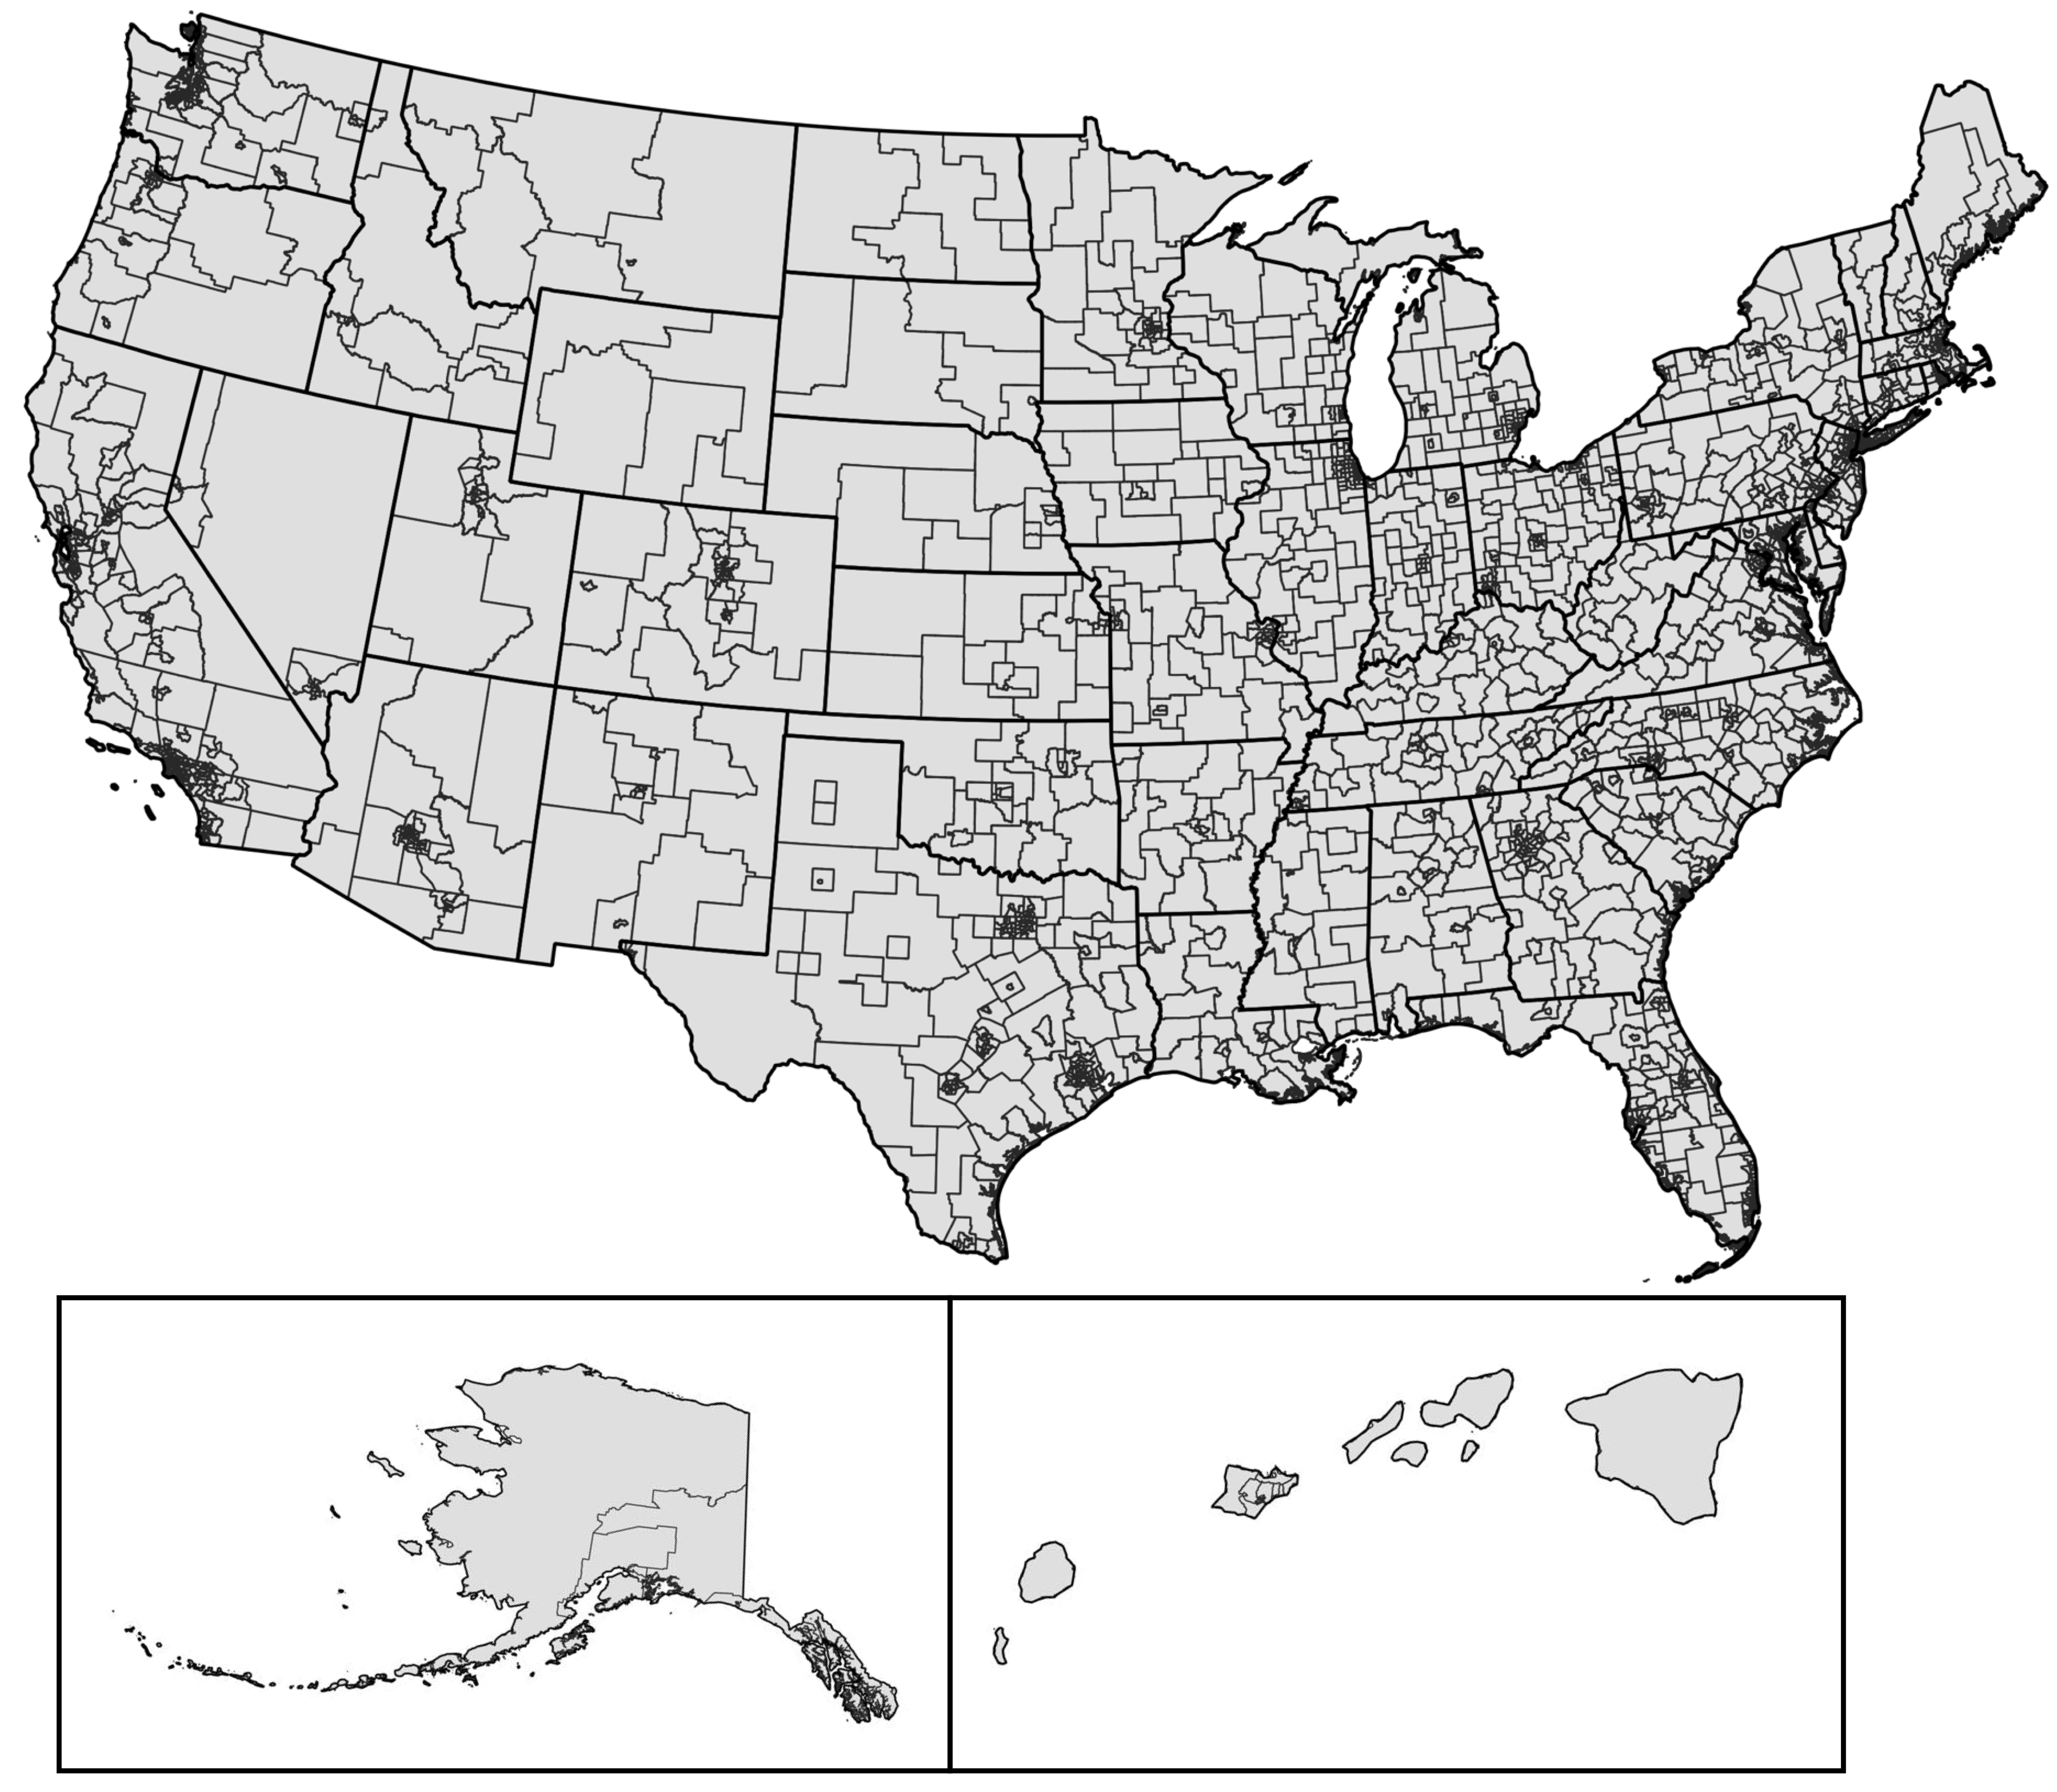
\includegraphics[width=1\linewidth]{images/2010-PUMAs.png}
    \caption{2010 Public Use Microdata Area boundaries}
    \label{fig:2010_puma_boundaries}
\end{figure}

\paragraph{Distribution Data Source(s)}
\begin{itemize} 
\item
  Spatial definitions are from the U.S.~Census Bureau as of July 1,
  2015.
\item
  Unit counts are from the American Community Survey 5-yr 2016.
\end{itemize}
\paragraph{Direct Conditional Dependencies}
\begin{itemize}
    \item County and PUMA.
\end{itemize}
\paragraph{Options}
The options for PUMAs are structured by their state abbreviation and the PUMA code from the GISJOIN code. The GISJOIN values are found in the 2010 TIGER/LINE Basis file on the \href{https://usa.ipums.org/usa/volii/boundaries.shtml}{IPUMS GIS Boundary Files}  website. An example is G01002100, which represents state FIPS code AL, and 02100 is the AL, Elmore, Autauga, Montgomery -Outer- and Lowndes Counties PUMA.

There are three ResStock arguments set with the PUMA options: \texttt{site\_elevation}, \texttt{site\_latitude}, and \texttt{site\_longitude}. All three of these arguments are set to ``auto'' and use the default \href{https://openstudio-hpxml.readthedocs.io/en/v1.8.1/workflow_inputs.html#hpxml-building-site}{OpenStudio-HPXML Building Site} values.

\begin{longtable}[]{ |p{3.cm}|p{1.5cm}|p{1cm}|p{1.1cm}|p{1.4cm}|p{6cm}| }
\caption{The ResStock argument definitions set in the PUMA characteristic} \label{table:hc_arg_def_puma}  \\
\toprule\noalign{}
Name & Required & Units & Type & Choices & Description \\
\midrule\noalign{}
\endhead
\bottomrule\noalign{}
\endlastfoot
\texttt{site\_elevation} & false & ft & Double & auto & Elevation of the
home address.  \\
\hline
\texttt{site\_latitude} & false & deg & Double & auto & Latitude of the
home address. Must be between -90 and 90. Use negative values for
southern hemisphere.\\
\hline
\texttt{site\_longitude} & false & deg & Double & auto & Longitude of
the home address. Must be between -180 and 180. Use negative values for
the western hemisphere.\\
\end{longtable}

\paragraph{Distribution Assumption(s)}
No assumptions are made.

\subsubsection{County and PUMA}
\paragraph{Description}
The GISJOIN identifier for the County and the PUMA where the sample is located. Since Counties and PUMAs are both a collection of census tracts, often a PUMA is in multiple counties. This characteristic describes the combination of County and PUMA where the sample is located.

\paragraph{Distribution Data Source(s)}
\begin{itemize}
 
\item
  Spatial definitions are from the U.S.~Census Bureau as of July 1,
  2015.
\item
  Unit counts are from the American Community Survey 5-yr 2016.
\end{itemize}

\paragraph{Direct Conditional Dependencies}
\begin{itemize}
    \item ASHRAE IECC Climate Zone 2004.
\end{itemize}
\paragraph{Options}
The options for County and PUMA are a combination of the NHGIS GISJOIN Code for the County and the PUMA separated by a comma. An example option is ``G0100010, G01002100''---G0100010 is the County GISJOIN for Autauga County, AL, and G01002100 is the PUMA GISJOIN for the AL, Elmore, Autauga, Montgomery -Outer- and Lowndes Counties PUMA.

\paragraph{Distribution Assumption(s)}
No assumptions are made.

\subsubsection{Metropolitan and Micropolitan Statistical Area}
\paragraph{Description}
The U.S.~Metropolitan Statistical Area (MSA) or Micropolitan Statistical Area (MicroSA) where sample is located. The U.S.~Census defines a set of counties as Core-Based Statistical Areas (CBSAs). These CBSAs are either assigned a MicroSA or combined into a larger MSA. According to the U.S.~Census, each metropolitan statistical area must have at least one urban area of 50,000 or more inhabitants. According to the U.S.~Census, each MicroSA must have at least one urban area of at least 10,000 but less than 50,000 population.

\paragraph{Distribution Data Source(s)}
\begin{itemize}
 
\item
  Spatial definitions are from the U.S.~Census Bureau as of July 1,
  2015.
\item
  Unit counts are from the American Community Survey 5-yr 2016.
\item
  County-MSA crosswalk comes from the Quarterly Census of Employment and
  Wages NAICS-based data between 2013 and 2022 by the U.S.~Bureau of Labor
  Statistics.
  (\url{https://www.bls.gov/cew/classifications/areas/county-msa-csa-crosswalk.htm})
\end{itemize}

\paragraph{Direct Conditional Dependencies}
\begin{itemize}
    \item County.
\end{itemize}

\paragraph{Options}
Options of the Metropolitan and Micropolitan Statistical Area characteristic are structured by having the name of the MSA or MicroSA, a comma, the State abbreviation, and either ``MSA'' or ``MicroSA.'' An example is ``Albany-Schenectady-Troy, NY MSA,'' which corresponds to the Albany-Schenectady-Troy MSA in New York State.

\paragraph{Distribution Assumption(s)}
No assumptions are made.

\subsubsection{City}
\paragraph{Description}
The City where the sample is located.

\paragraph{Distribution Data Source(s)}
\begin{itemize}
 
\item
  Spatial definitions are from the U.S.~Census Bureau as of July 1,
  2015.
\item
  Cities are defined by Census blocks by their Census Place in the 2010
  Census.
\item
  Unit counts are from the American Community Survey 5-yr 2016.
\end{itemize}

\paragraph{Direct Conditional Dependencies}
\begin{itemize}
    \item County and PUMA.
\end{itemize}

\paragraph{Options}
The options are structured as the State abbreviation of the city, a comma, and the name of the city. An example is ``AR, Jonesboro,'' which corresponds to Jonesboro, Arkansas.

The ResStock argument \texttt{site\_city} is assigned in the City characteristic. The argument is set to ``auto,'' which is the OpenStudio-HPXML default value; see the OpenStudio-HPXML \href{https://openstudio-hpxml.readthedocs.io/en/v1.8.1/workflow_inputs.html#hpxml-building-site}{Building Site} section of the documentation for the default values.

\begin{longtable}[]{ |p{3.cm}|p{1.5cm}|p{1.1cm}|p{6cm}| }
\caption{The ResStock argument definitions set in the City characteristic} \label{table:hc_arg_def_city}  \\
\toprule\noalign{}
Name & Required & Type  & Description \\
\midrule\noalign{}
\endhead
\bottomrule\noalign{}
\endlastfoot
\texttt{site\_city} & false & String & City/municipality of the home
address. \\
\end{longtable}

\paragraph{Distribution Assumption(s)}
\begin{itemize}
\item
  2020 Decennial Redistricting data were used to map tract-level unit
  counts to census blocks.
\item
  1,099 cities are tagged in ResStock, but there are over 29,000 Places
  in the Census data.
\item
  The threshold for including a Census Place in the City characteristic is 15,000 housing units.
\item
  The value ``In another census Place'' designates the fraction of housing units in a Census Place with fewer total housing units than the threshold.
\item
  The value ``Not in a census Place''
  designates the fraction of housing units not in a Census Place
  according to the 2010 Census.
\end{itemize}


\subsubsection{AIANNH Area}
\paragraph{Description}
American Indian/Alaska Native/Native Hawaiian (AIANNH) Area where the sample is located. See Figure \ref{fig:aiannh_map} for a map of AIANNH areas in the contiguous United States.

\begin{figure}
    \centering
    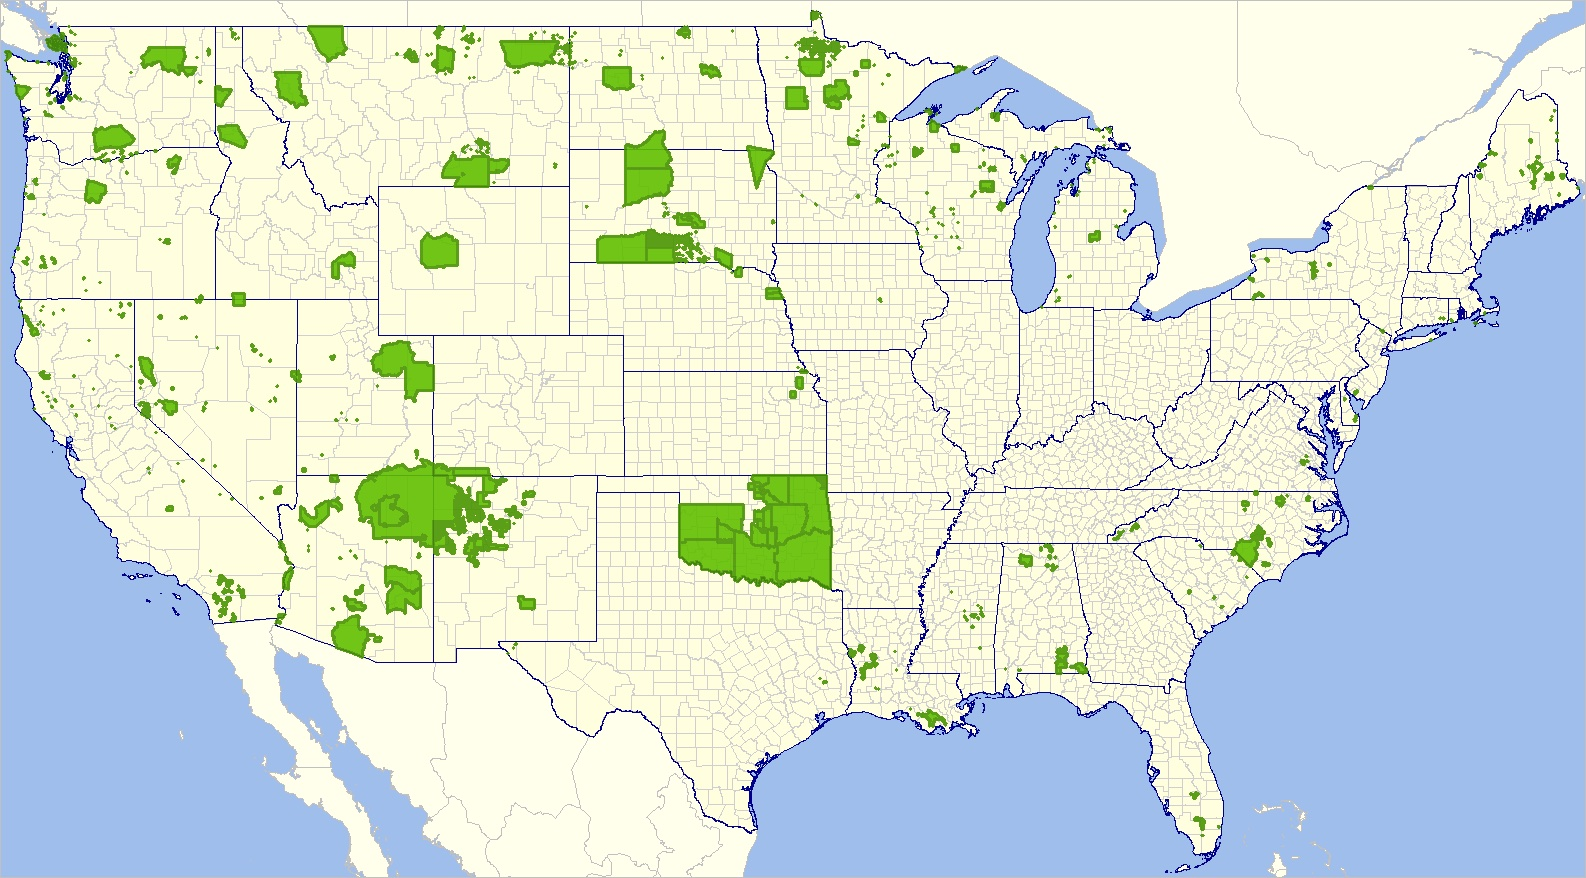
\includegraphics[width=1\linewidth]{images/aiannh_48b.jpg}
    \caption{AIANNH area map. The image is created by \href{https://proximityone.com/aiannh.htm}{ProximityOne} and excludes Alaska and Hawaii.}
    \label{fig:aiannh_map}
\end{figure}


\paragraph{Distribution Data Source(s)}
\begin{itemize}
    \item 2010 Census Tract to American Indian Area (AIA) Relationship File provides the percent housing units in the census tract that belong to AIA. 
    \item Spatial definitions are from the U.S.~Census Bureau as of July 1, 2015.
    \item Unit counts are from the American Community Survey 5-yr 2016.
\end{itemize}

\paragraph{Direct Conditional Dependencies}
\begin{itemize}
    \item County and PUMA.
\end{itemize}

\paragraph{Options}
The options are either ``Yes'' or ``No,'' indicating if the housing unit is in an AIANNH area.

\paragraph{Distribution Assumption(s)}
\begin{itemize}
    \item The 2010 Census Tracts are mapped to 2015 County and PUMA by adjusting for known geographic changes (e.g., renaming of Shannon County to Oglala Lakota County, SD) However, Tract=G3600530940103 (Oneida city, Madison County, NY) could not be mapped to County and PUMA and was removed. The tract contains only 11 units for AIA.
\end{itemize}

\subsubsection{County Metro Status}
\paragraph{Description}
The Metro Status of the county where the sample is located and is based on MSA and MicroSA.

\paragraph{Distribution Data Source(s)}
\begin{itemize}
    \item Spatial definitions are from the U.S.~Census Bureau as of July 1, 2015.
    \item Unit counts are from the American Community Survey 5-yr 2016.
    \item County-MSA crosswalk comes from the Quarterly Census of Employment and Wages NAICS-based data between 2013 and 2022 by the U.S.~Bureau of Labor Statistics \href{https://www.bls.gov/cew/classifications/areas/county-msa-csa-crosswalk.htm}{U.S.~Bureau of Labor Statistics}.
\end{itemize}

\paragraph{Direct Conditional Dependencies}
\begin{itemize}
    \item Metropolitan and Micropolitan Statistical Area.
\end{itemize}

\paragraph{Options}
The options are either ``Metropolitan'' or ``Non-Metropolitan.''

\paragraph{Distribution Assumption(s)}
No assumptions are made.


\subsubsection{PUMA Metro Status}
\paragraph{Description}
The PUMA metropolitan status where the housing unit is located.

\paragraph{Distribution Data Source(s)}
\begin{itemize}
    \item 2019-5yrs Public Use Microdata Samples (PUMS). IPUMS USA, University of Minnesota, www.ipums.org.
\end{itemize}

\paragraph{Direct Conditional Dependencies}
\begin{itemize}
    \item PUMA.
\end{itemize}

\paragraph{Options}
The options are either (1) In metro area, not/partially in principal city, (2) In metro area, principal city, or (3) Not/partially in metro area. 

\paragraph{Distribution Assumption(s)}
\begin{itemize}
    \item The PUMA Metro Status, derived from ACS IPUMS METRO codes, indicates whether the household resided within a metropolitan area and, for households in metropolitan areas, whether the household resided within or outside of a central/principal city. Each PUMA has a unique METRO status in ACS and therefore has a unique PUMA Metro Status. IPUMS derives METRO codes for samples not directly identified based on available geographic information and whether the associated county group or PUMA lies wholly or only partially within metropolitan areas or principal cities.
\end{itemize}

\subsection{Climate Zones}
This section of ResStock characteristics is a set of Climate Zone definitions. There are five input files to ResStock that specify climate zones:
\begin{itemize}
    \item ASHRAE IECC Climate Zone 2004
    \item ASHRAE IECC Climate Zone 2004---2A Split
    \item Building America Climate Zones
    \item California Energy Commission (CEC) Climate Zones
    \item ENERGY STAR\textsuperscript{\textregistered} Climate Zone 2023.
\end{itemize}
\subsubsection{ASHRAE IECC Climate Zone 2004} \label{sec:ashrae_2004_tsv}
\paragraph{Description}
Climate zone according to ASHRAE 169 in 2004 and IECC in 2012 where the sample is located. See Figure \ref{fig:ashrae_169_2004_cz} for a map of the climate zones.

\begin{figure}
    \centering
    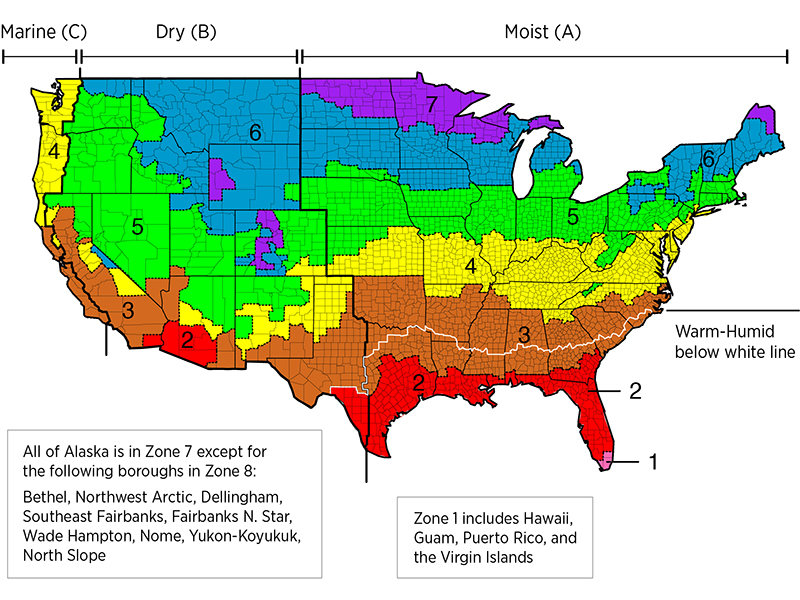
\includegraphics[width=1\linewidth]{images/ashrae_iecc_cz_map_2004.jpg}
    \caption{The 2004 ASHRAE 169 and IECC 2012 climate zone map}
    \label{fig:ashrae_169_2004_cz}
\end{figure}

\paragraph{Distribution Data Source(s)}
\begin{itemize}
    \item Spatial definitions are from the U.S.~Census Bureau as of July 1, 2015.
    \item Unit counts are from the American Community Survey 5-yr 2016.
    \item Climate zone data are from ASHRAE 169 2004, IECC 2012, and \href{https://www.energy.gov/sites/prod/files/2015/10/f27/ba_climate_region_guide_7.3.pdf}{M.C. Baechler 2015}.
\end{itemize}

\paragraph{Direct Conditional Dependencies}
There are no direct conditional dependencies.

\paragraph{Options}
A set of counties defines each climate and moisture zone. Climate zones range from 1--8 and moisture zones are indicated by A, B, and C. 

The ASHRAE IECC Climate Zone 2004 sets the \texttt{site\_type} and \texttt{site\_iecc\_zone} arguments. The \texttt{site\_type} is always set to ``auto.'' The \texttt{site\_iecc\_zone} argument matches the climate zone with the exception of climate zones 7 and 8 in Alaska. ResStock departs from the climate zone definitions by using 7AK and 8AK instead of 7 and 8 from the standards.

\begin{customLongTable}{ |p{3.cm}|p{1.5cm}|p{1.1cm}|p{4.4cm}|p{4cm}| }
{The ResStock arguments set in the ASHRAE IECC Climate Zone 2004 characteristic} {table:hc_arg_def_ashrae_2004}  
{Name & Required & Type & Choices & Description} 
\texttt{site\_type} & false & Choice & auto, suburban, urban, rural &
The type of site.  \\
\hline
\texttt{site\_iecc\_zone} & false & Choice & auto, 1A, 1B, 1C, 2A, 2B,
2C, 3A, 3B, 3C, 4A, 4B, 4C, 5A, 5B, 5C, 6A, 6B, 6C, 7, 8 & IECC zone of
the home address. \\
\end{customLongTable}

\paragraph{Distribution Assumption(s)}
No assumptions are made.

\subsubsection{ASHRAE IECC Climate Zone 2004---2A Split}
\paragraph{Description}
The climate zone, according to ASHRAE 169 in 2004 and IECC in 2012, where the sample is located. Climate zone where climate zone 2A is split between counties in (1) TX and LA, and (2) FL, GA, AL, and MS. See Figure \ref{fig:ashrae_169_2004_cz} for the climate zones and the climate zone 2A counties that are split between the states mentioned previously.

\paragraph{Distribution Data Source(s)}
\begin{itemize}
    \item Spatial definitions are from the U.S.~Census Bureau as of July 1, 2015.
    \item Unit counts are from the American Community Survey 5-yr 2016.
    \item Climate zone data are from ASHRAE 169 2004, IECC 2012, and \href{https://www.energy.gov/sites/prod/files/2015/10/f27/ba_climate_region_guide_7.3.pdf}{M.C. Baechler 2015}.
\end{itemize}

\paragraph{Direct Conditional Dependencies}
\begin{itemize}
    \item County.
\end{itemize}

\paragraph{Options}
A set of counties defines each climate and moisture zone. Climate zones range from 1--8 and moisture zones are indicated by A, B, and C. Climate zone 2A is split between options ``2A---FL, GA, AL, MS'' and ``2A---TX, LA.''

\paragraph{Distribution Assumption(s)}
\begin{itemize}
    \item This characteristic is used to better represent HVAC types in the 2A climate zone.
\end{itemize}

\subsubsection{Building America Climate Zones}
\paragraph{Description}
The Building America Climate Zone where the sample is located. See Figure \ref{fig:building_america_cz} for a map of the climate zones. \footnote{The Subarctic climate zone is not shown and is only found in Alaska.}

\begin{figure}
    \centering
    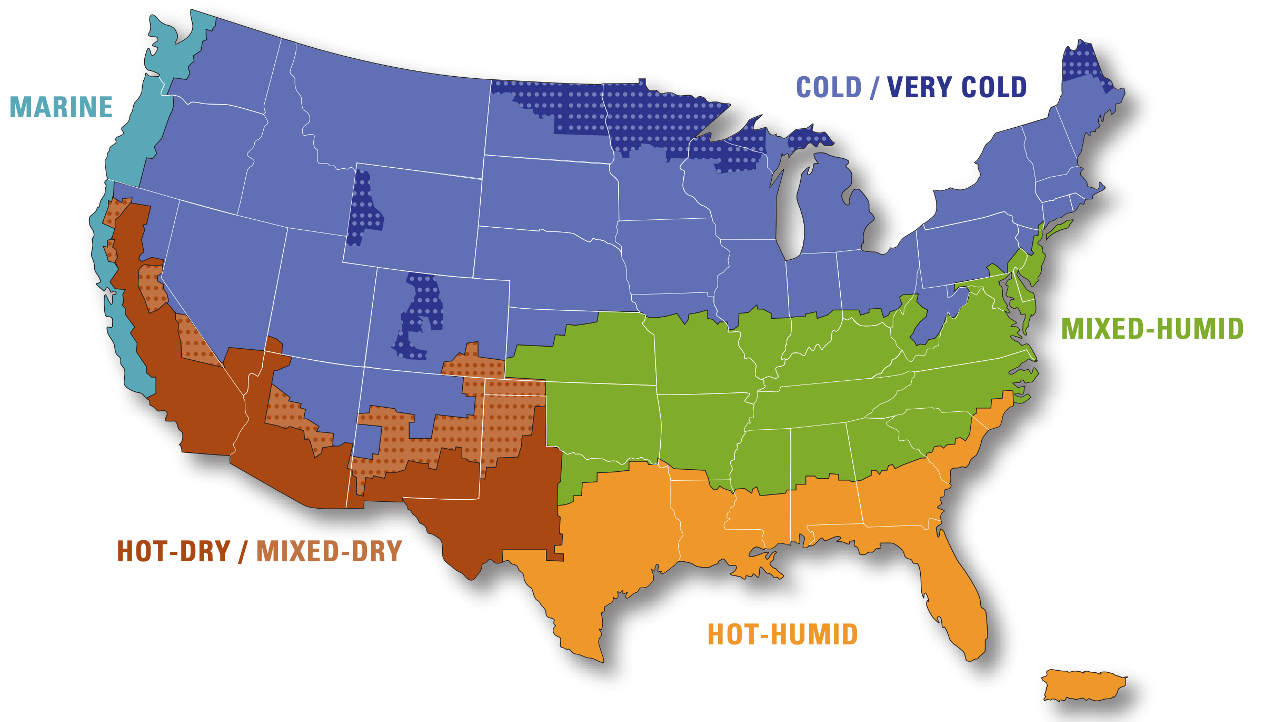
\includegraphics[width=1\linewidth]{images/building_america_cz.png}
    \caption{Building America Climate Zone map}
    \label{fig:building_america_cz}
\end{figure}

\paragraph{Distribution Data Source(s)}
\begin{itemize}
    \item Unit counts are from the American Community Survey 5-yr 2016.
    \item Spatial definitions are from U.S.~Census 2010.
    \item Climate zone data are from ASHRAE 169 2004, IECC 2012, and \href{https://www.energy.gov/sites/prod/files/2015/10/f27/ba_climate_region_guide_7.3.pdf}{M.C. Baechler 2015}.
\end{itemize}

\paragraph{Direct Conditional Dependencies}
\begin{itemize}
    \item County.
\end{itemize}

\paragraph{Options}
The options for the Building America Climate Zone characteristic are the same as the climate zones: Cold, Hot-Dry, Hot-Humid, Marine, Mixed-Dry, Mixed-Humid, Subarctic, and Very Cold.

\paragraph{Distribution Assumption(s)}
No assumptions are made.

\subsubsection{California Energy Commission Climate Zones}
\paragraph{Description}
The CEC Climate Zone where the sample is located. See Figure \ref{fig:cec_cz} for a map of the CEC building climate zones.

\begin{figure}
    \centering
    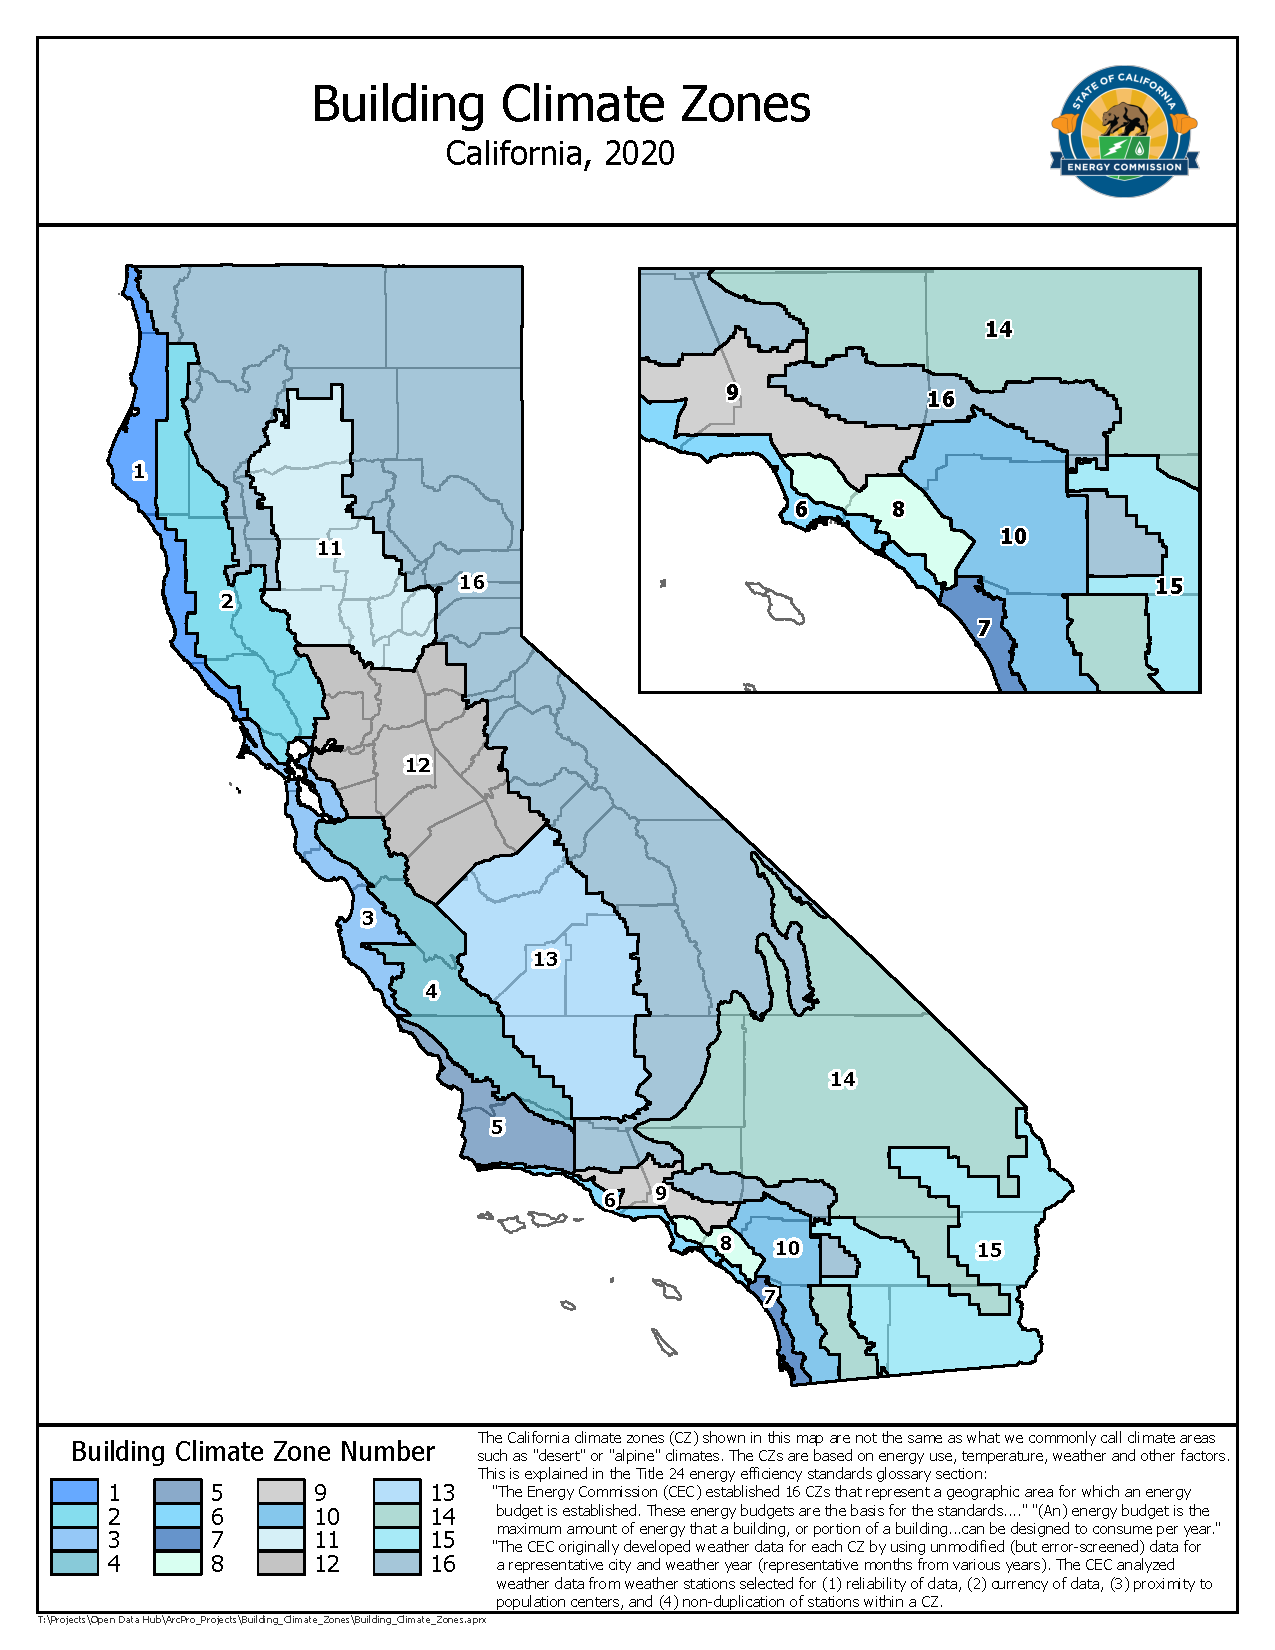
\includegraphics[width=1\linewidth]{images/CEC_Building_Climate_Zones.pdf}
    \caption{California Energy Commission \href{https://cecgis-caenergy.opendata.arcgis.com/documents/CAEnergy::building-climate-zones/explore}{Building Climate Zone map}}
    \label{fig:cec_cz}
\end{figure}

\paragraph{Distribution Data Source(s)}
\begin{itemize}
    \item Spatial definitions are from the U.S.~Census Bureau as of July 1, 2015.
    \item Zip code definitions are from the end of Q2 2020.
    \item The climate zone to zip codes in California is from the CEC Website.
\end{itemize}

\paragraph{Direct Conditional Dependencies}
\begin{itemize}
    \item County and PUMA.
\end{itemize}

\paragraph{Options}
The options range from 1--16 in California. For other states, the option is set to None.

\paragraph{Distribution Assumption(s)}
\begin{itemize}
    \item CEC Climate zones are defined by Zip Codes.
    \item The dependency selected is County and PUMA as zip codes are not modeled in ResStock.
    \item The mapping between Census Tracts and Zip Codes is approximate and some discrepancies may exist.
\end{itemize}

\subsubsection{ENERGY STAR Climate Zone 2023}
\paragraph{Description}
Climate zones for windows, doors, and skylights per ENERGY STAR guidelines as of 2023. See Figure \ref{fig:energy_star_cz} for a map of the climate zones.

\begin{figure}
    \centering
    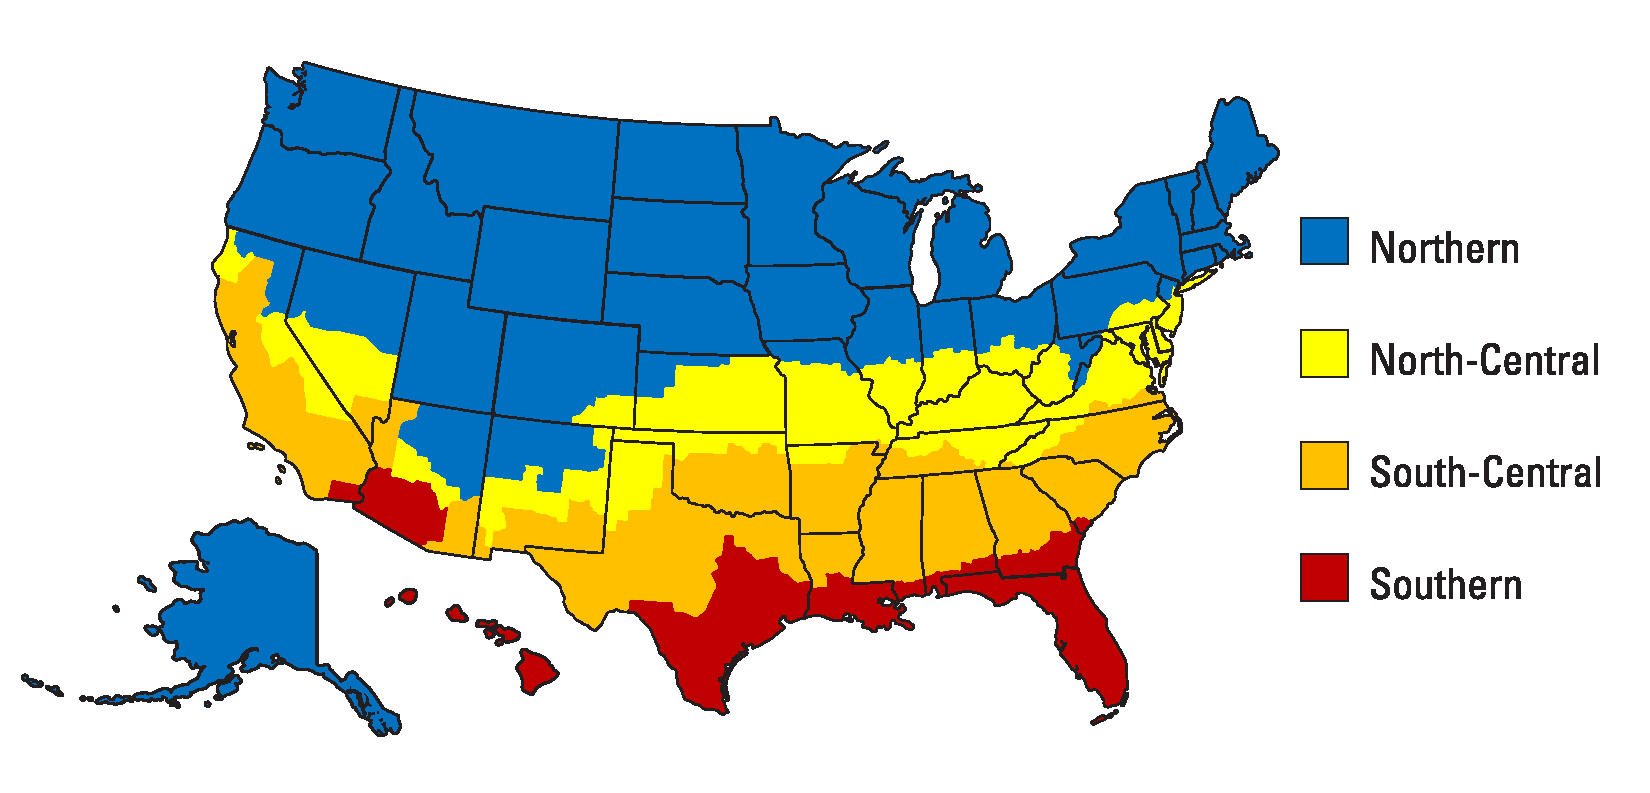
\includegraphics[width=1\linewidth]{images/ENERGY_STAR_Climate_Zone_Map.pdf}    \caption{\href{https://www.energystar.gov/sites/default/files/asset/document/Promotional_Map.pdf}{ENERGY STAR V7 climate zone} map}
    \label{fig:energy_star_cz}
\end{figure}

\paragraph{Distribution Data Source(s)}
\begin{itemize}
    \item Area definition approximated based on published map retrieved in May 2023 from the \href{https://www.energystar.gov/products/residential_windows_doors_and_skylights/key_product_criteria}{ENERGY STAR windows, doors, and skylights key product criteria} website. 
\end{itemize}

\paragraph{Direct Conditional Dependencies}
\begin{itemize}
    \item CEC Climate Zone
    \item County.
\end{itemize}

\paragraph{Options}
The options for the ENERGY STAR climate Zone 2023 characteristic are the same as climate zones: North-Central, Northern, South-Central, and Southern. 

\paragraph{Distribution Assumption(s)}
\begin{itemize}
    \item ENERGY STAR Climate Zones assigned based on CEC Climate Zone for California and based on County everywhere else.
\end{itemize}

\subsection{Grid and Emissions Geographies}

In ResStock there are three input files describing geographies relevant to the electric grid and emissions calculations:

\begin{itemize}
    \item ReEDS Balancing Area
    \item Generation and Emissions Assessment (GEA) Region
    \item ISO RTO Region.
\end{itemize}

\subsubsection{ReEDS Balancing Area}
\paragraph{Description}
The Regional Energy Deployment System Model (ReEDS) balancing area where the sample is located. See Figure \ref{fig:reeds_ba_map} to see a map of the balancing areas.

\begin{figure}
    \centering
    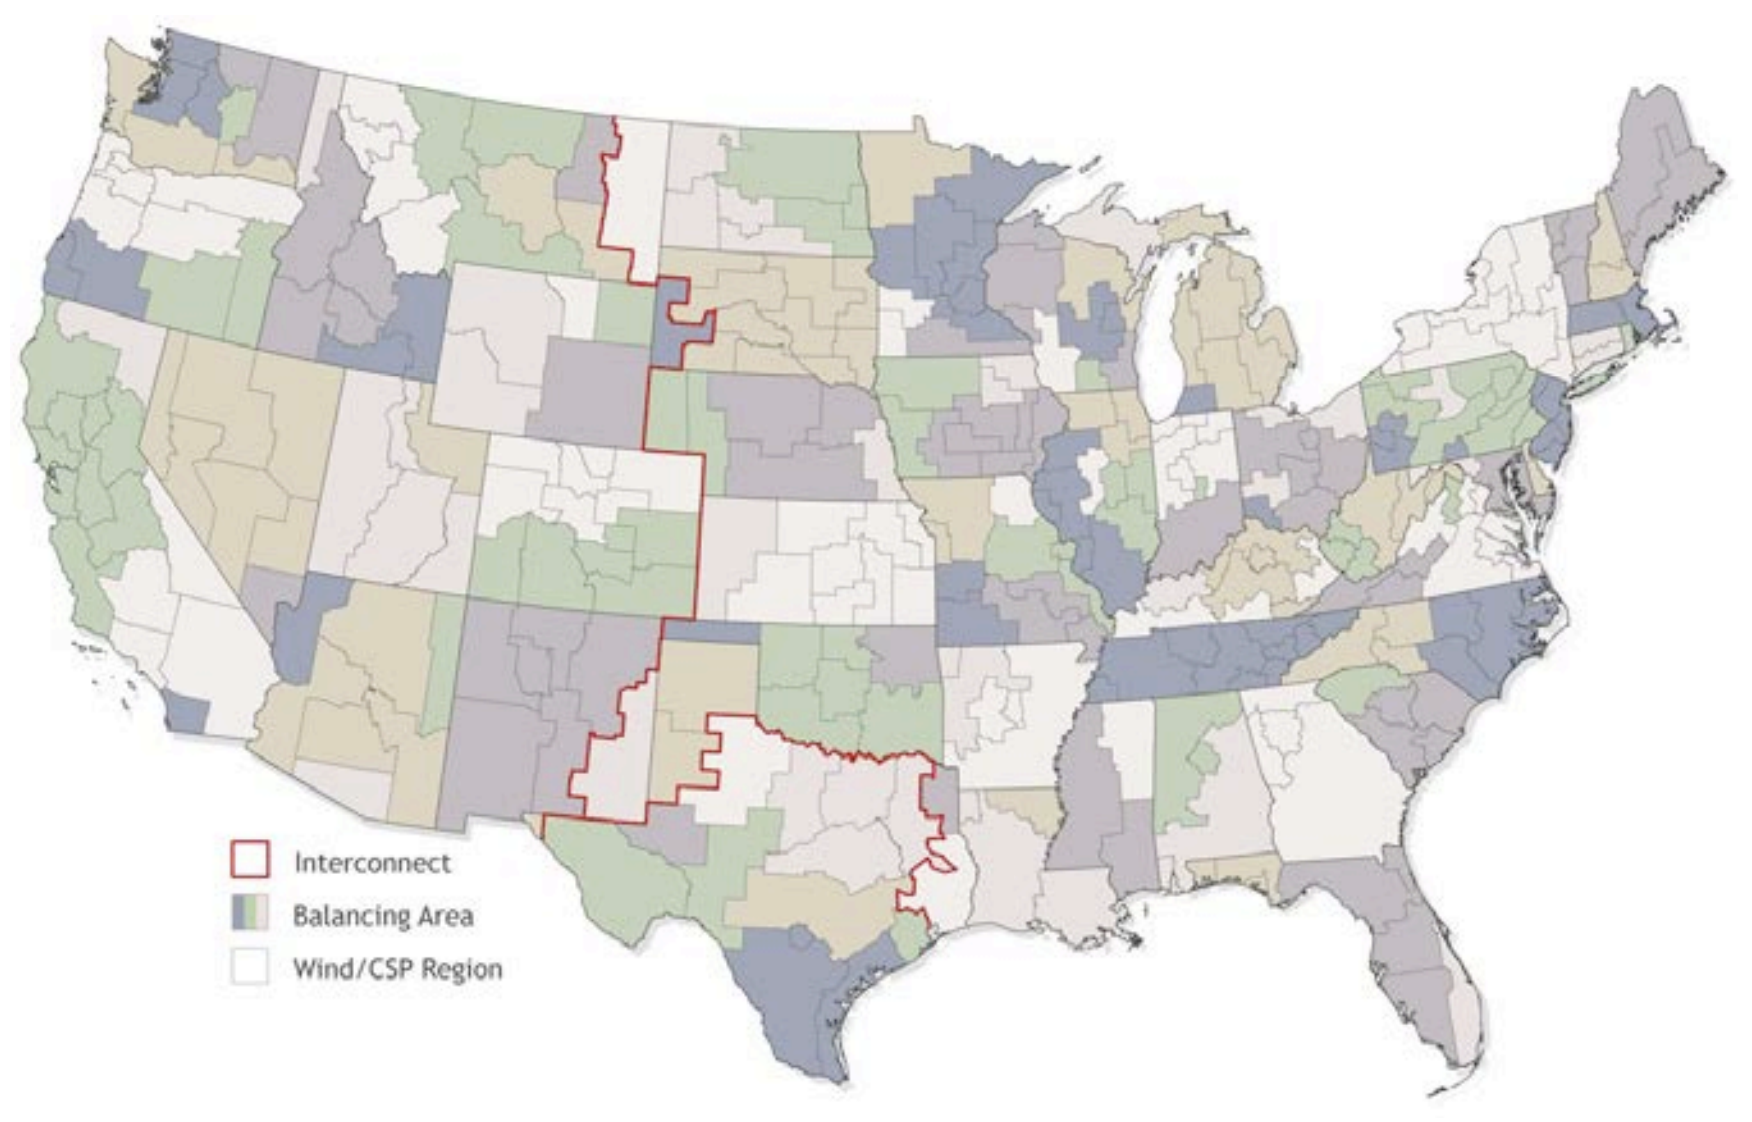
\includegraphics[width=1\linewidth]{images/reeds_ba_map.png}
    \caption{ReEDS balancing area map}
    \label{fig:reeds_ba_map}
\end{figure}

\paragraph{Distribution Data Source(s)}
\begin{itemize}
    \item Spatial definitions are from the U.S.~Census Bureau as of July 1, 2015.
    \item Unit counts are from the American Community Survey 5-yr 2016.
    \item Brown, Maxwell, Wesley Cole, Kelly Eurek, Jon Becker, David Bielen, Ilya Chernyakhovskiy, Stuart Cohen et al. 2020. Regional Energy Deployment System (ReEDS) Model Documentation: Version 2019. Golden, CO: National Renewable Energy Laboratory. NREL/TP-6A20-74111. https://www.nrel.gov/docs/fy20osti/74111.pdf.
\end{itemize}

\paragraph{Direct Conditional Dependencies}
\begin{itemize}
    \item County
\end{itemize}
\paragraph{Options}
The options for the ReEDS Balancing Area characteristic is a set of integers 1-134 based on Figure \ref{fig:reeds_ba_map}. Alaska and Hawaii do not have a ReEDS balancing area and are labeled with the None option.
\paragraph{Distribution Assumption(s)}
No assumptions are made.

\subsubsection{Generation and Emissions Assessment (GEA) Region}
\paragraph{Description}
The 2021 Cambium generation and carbon emissions assessment region where the sample is located. See Figure \ref{fig:cambium_gea_map} for a map of these regions.

\begin{figure}
    \centering
    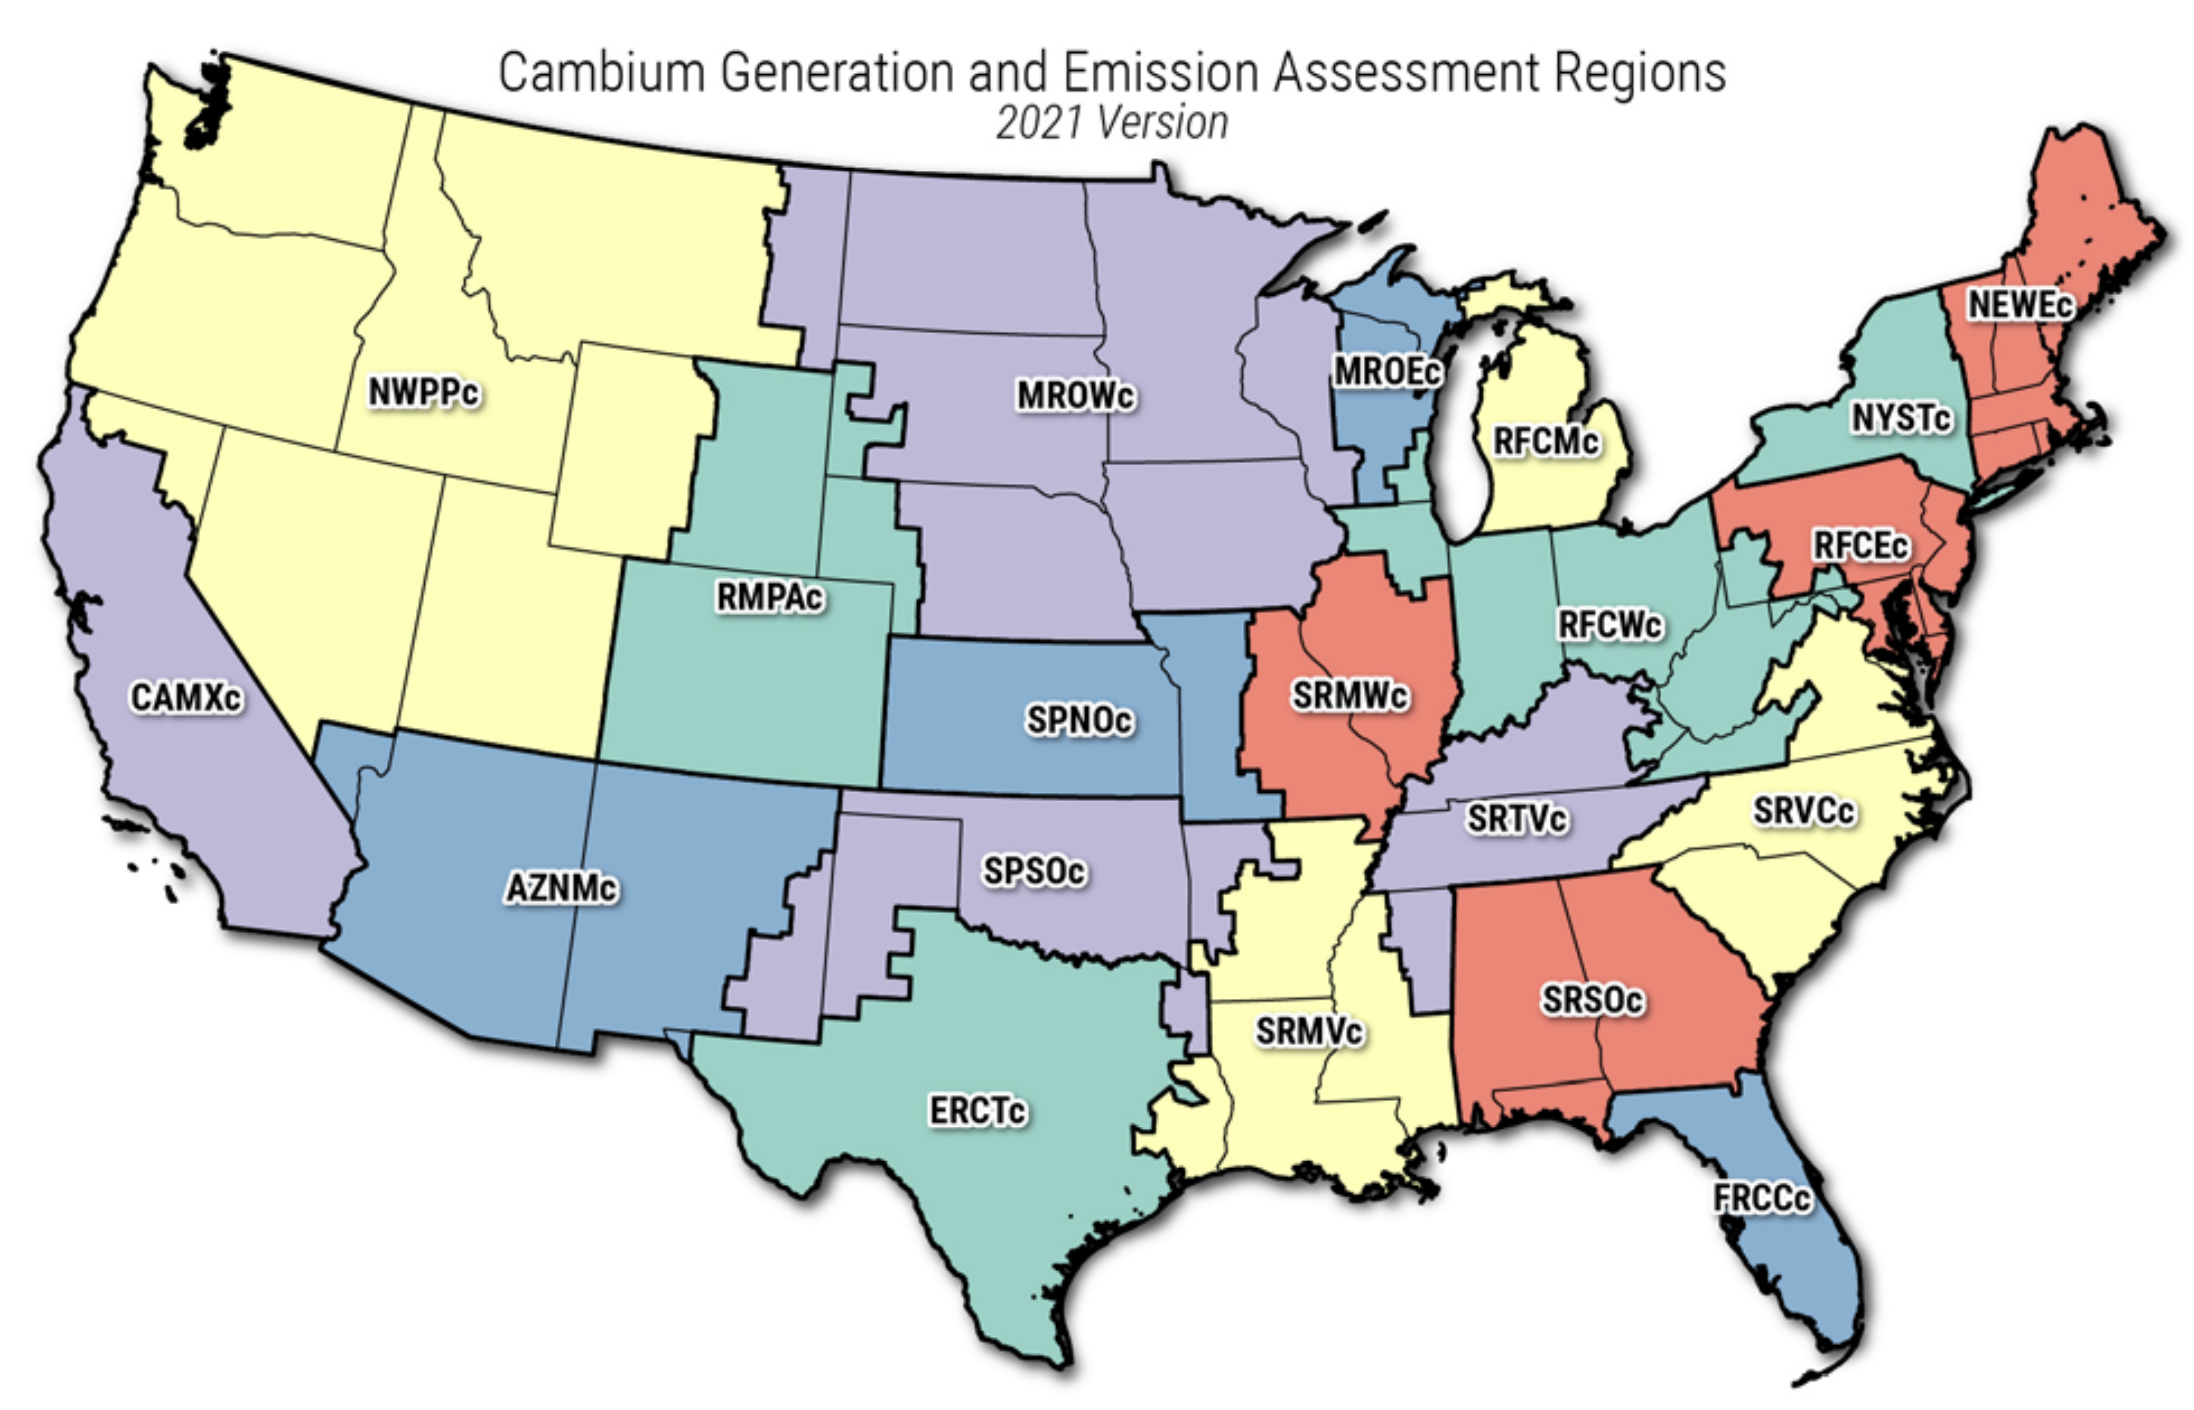
\includegraphics[width=1\linewidth]{images/Cambium_GEAs_2021.png}
    \caption{ Map of the \href{https://www.nrel.gov/analysis/cambium.html}{Cambium} 2021 Generation and Emission Assessment Regions.}
    \label{fig:cambium_gea_map}
\end{figure}

\paragraph{Distribution Data Source(s)}
\begin{itemize}
    \item Pieter Gagnon, Will Frazier, Wesley Cole, and Elaine Hale. 2021. Cambium Documentation: Version 2021. Golden, CO.: National Renewable Energy Laboratory. NREL/TP-6A40-81611. https://www.nrel.gov/docs/fy22osti/81611.pdf
\end{itemize}

\paragraph{Direct Conditional Dependencies}
\begin{itemize}
    \item REEDS Balancing Area
\end{itemize}

\paragraph{Options}
The options follow the Cambium GEA region names: AZNMc, CAMXc, ERCTc, FRCCc, MROEc, MROWc, NEWEc, NWPPc, NYSTc, RFCEc, RFCMc, RFCWc, RMPAc, SPNOc, SPSOc, SRMVc, SRMWc, SRSOc, SRTVc, and SRVCc. The None option is set for Alaska and Hawaii as these states do not have a ReEDS balancing area.

\paragraph{Distribution Assumption(s)}
No assumptions are made.

\subsubsection{ISO RTO Region}
\paragraph{Description}
The independent system operator (ISO) or regional transmission organization (RTO) region where the sample is located.

\paragraph{Distribution Data Source(s)}
\begin{itemize}
    \item Spatial definitions are from the U.S.~Census Bureau as of July 1, 2015.
    \item Unit counts are from the American Community Survey 5-yr 2016.
    \item ISO and RTO regions are from EIA Form 861, 2018.
\end{itemize}

\paragraph{Direct Conditional Dependencies}
\begin{itemize}
    \item County
\end{itemize}

\paragraph{Options}
The options are a list of options that represent ISOs and RTOs:
\begin{itemize}
    \item Pennsylvania New Jersey Maryland Interconnection (PJM)
    \item Midcontinent Independent System Operator (MISO)
    \item Electric Reliability Council of Texas (ERCOT)
    \item California ISO (CAISO)
    \item New York ISO (NYISO)
    \item Southwest Power Pool (SPP)
    \item ISO New England (NEISO)
\end{itemize}
If the county is not in any of these regions, the option is listed as the None option.

\paragraph{Distribution Assumption(s)}
No assumptions were made.

\subsection{Other Geographies}

In this section, we cover other miscellaneous geographies in ResStock. This includes four input files:
\begin{itemize}
    \item Census Division RECS
    \item Custom State
    \item Location Region
    \item American Housing Survey Region
\end{itemize}

\subsubsection{Census Division RECS}
\paragraph{Description}
Census Division as used in RECS 2015 where the sample is located.

\paragraph{Distribution Data Source(s)}
\begin{itemize}
    \item Spatial definitions are from the U.S.~Census Bureau as of July 1, 2015.
    \item Unit counts are from the American Community Survey 5-yr 2016.
    \item U.S.~EIA 2015 Residential Energy Consumption Survey (RECS) codebook.
\end{itemize}

\paragraph{Direct Conditional Dependencies}
\begin{itemize}
    \item State
\end{itemize}

\paragraph{Options}
The options match the names of the Census divisions except for RECS 2015 splits the Mountain Census Division into North (CO, ID, MT, UT, WY) and South (AZ, NM, NV).

\paragraph{Distribution Assumption(s)}
No assumptions were made.

\subsubsection{Custom State}
\paragraph{Description}
A custom selection of states to be able to have more fine-tuned probability distribution in states where we have more data.

\paragraph{Distribution Data Source(s)}
No data sources were used.

\paragraph{Direct Conditional Dependencies}
\begin{itemize}
    \item State
\end{itemize}
\paragraph{Options}
The options for the Custom State characteristic are "AK" and "Others". The characteristic was added during the calibration of Alaska to integrate the Alaska Retrofit Information System data.

\paragraph{Distribution Assumption(s)}
No assumptions were made.

\subsubsection{Location Region}
\paragraph{Description}
A custom ResStock region constructed of EIA RECS 2009 reportable domains where the sample is located. See Figure \ref{fig:location_region_map} for a map of these regions.

\begin{figure}
    \centering
    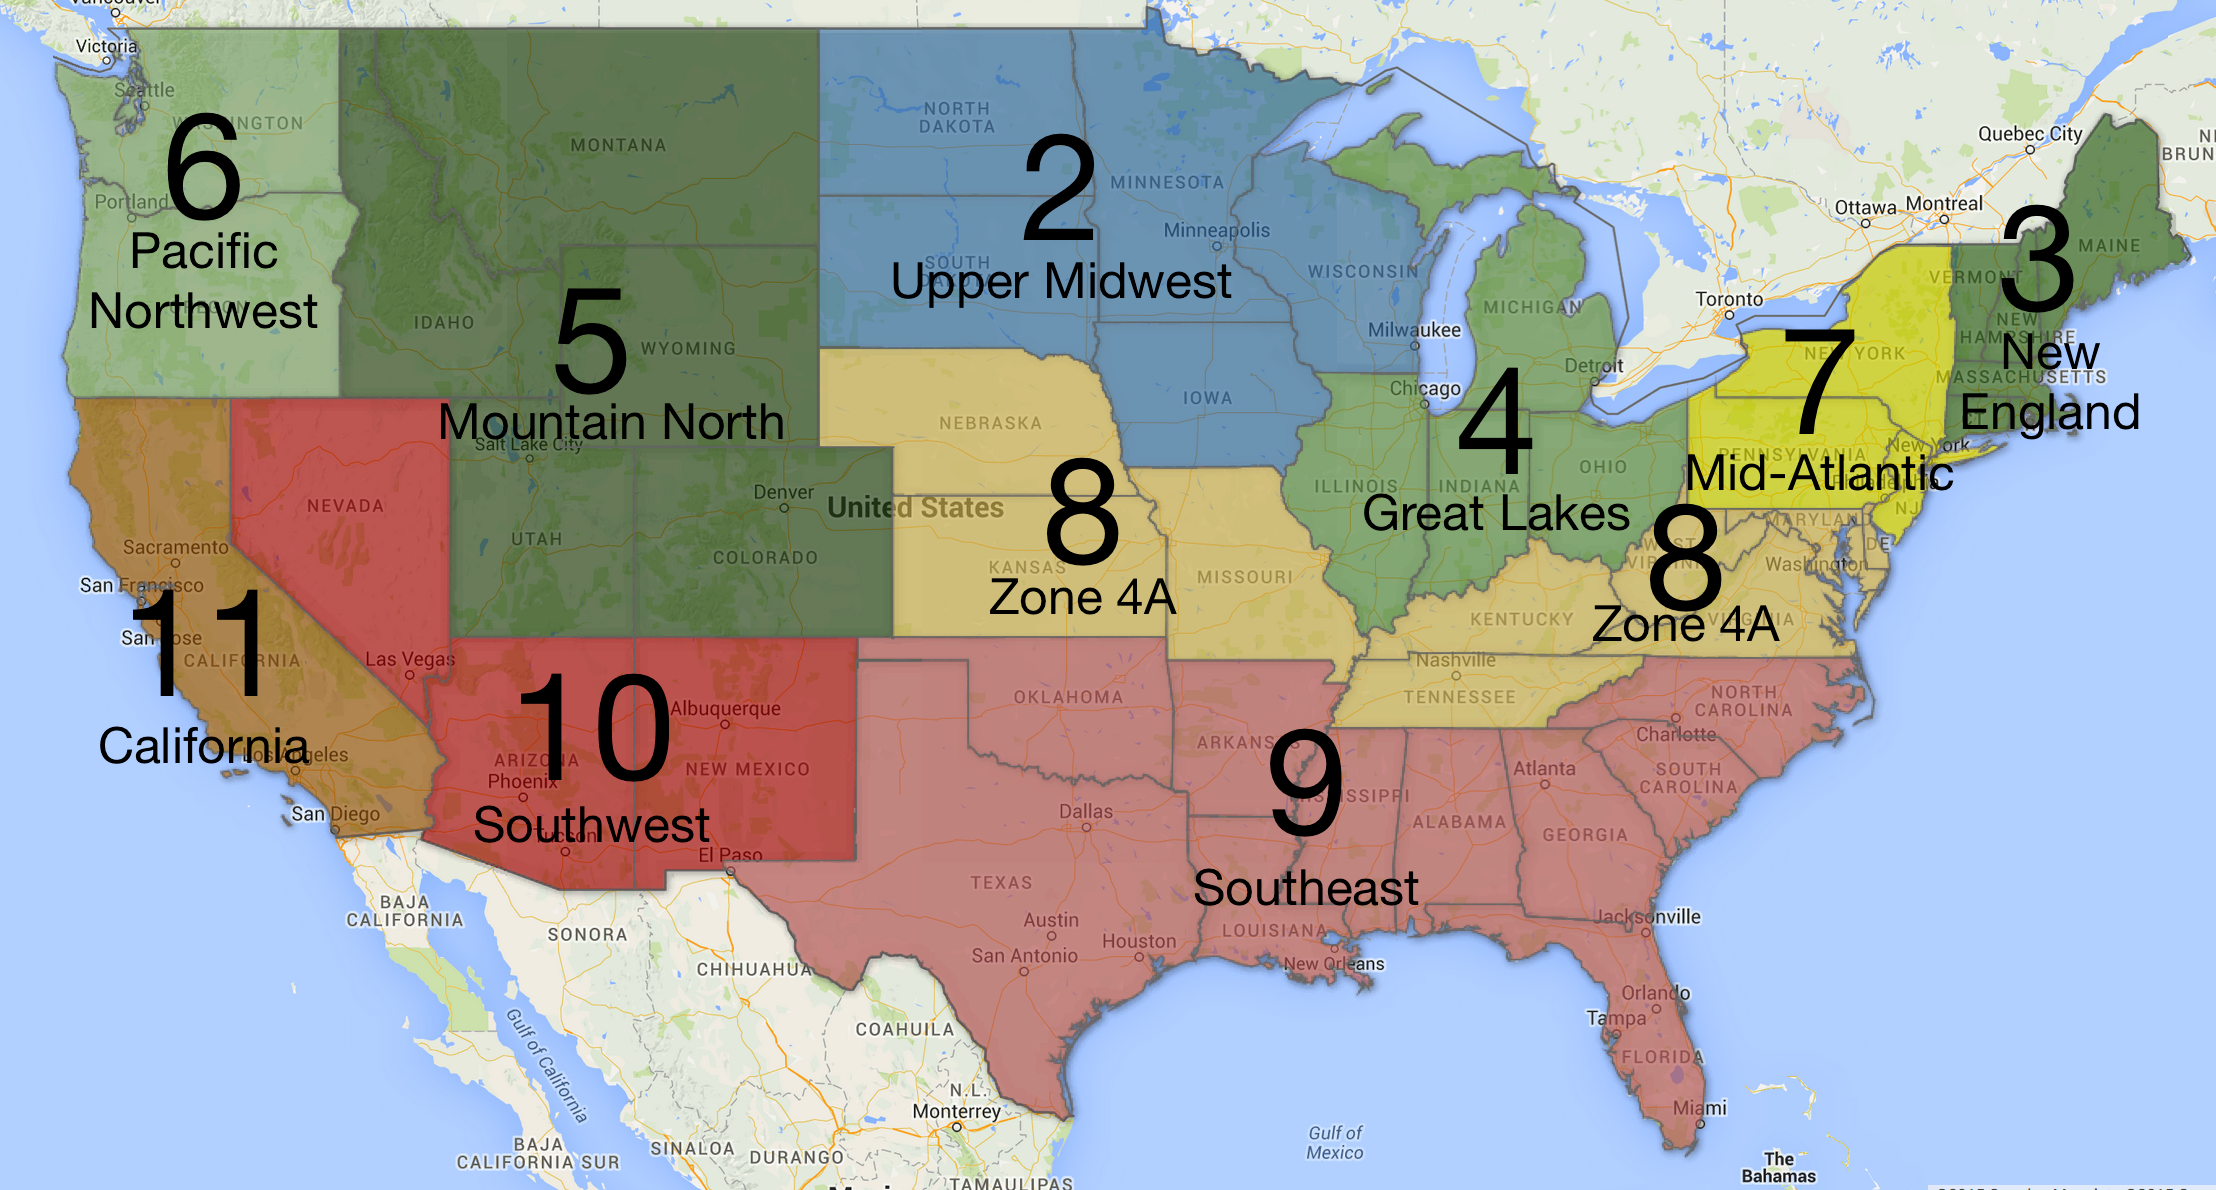
\includegraphics[width=1\linewidth]{images/custom_region_map.png}
    \caption{ Map of the custom regions in ResStock. Alaska and Hawaii are their own custom regions.}
    \label{fig:location_region_map}
\end{figure}


\paragraph{Distribution Data Source(s)}
\begin{itemize}
    \item Spatial definitions are from the U.S.~Census Bureau as of July 1, 2015.
    \item Unit counts are from the American Community Survey 5-yr 2016.
    \item U.S.~EIA 2009 Residential Energy Consumption Survey (RECS) microdata.
\end{itemize}

\paragraph{Direct Conditional Dependencies}
\begin{itemize}
    \item State
\end{itemize}

\paragraph{Options}
A list of custom regions (CRs) that range from CR02 - CR11. These numbered CRs are the historical options of the contiguous United States. When Alaska and Hawaii were added, CRAK and CRHI options were added, respectively.

\paragraph{Distribution Assumption(s)}
No assumptions are made.

\subsubsection{American Housing Survey Region}
\paragraph{Description}
The American Housing Survey region where the sample is located.

\paragraph{Distribution Data Source(s)}
\begin{itemize}
    \item Spatial definitions are from the U.S.~Census Bureau as of July 1, 2015.
    \item Unit counts are from the American Community Survey 5-yr 2016.
    \item Core Based Statistical Area (CBSA) data based on the Feb 2013 CBSA delineation file.
    \item 2013 American Housing Survey microdata.
\end{itemize}

\paragraph{Direct Conditional Dependencies}
\begin{itemize}
    \item County
\end{itemize}

\paragraph{Options}
Using the American Housing Survey microdata, 15 of the largest core-based statistical areas (CBSAs) were separated from their census divisions. This process resulted in 15 CBSA geographies and 9 Census Division Geographies that do not include the list of largest CBSAs. The list of options are: CBSA Atlanta-Sandy Springs-Roswell, GA; CBSA Boston-Cambridge-Newton, MA-NH; CBSA Chicago-Naperville-Elgin, IL-IN-WI; CBSA Dallas-Fort Worth-Arlington, TX; CBSA Detroit-Warren-Dearborn, MI; CBSA Houston-The Woodlands-Sugar Land, TX; CBSA Los Angeles-Long Beach-Anaheim, CA; CBSA Miami-Fort Lauderdale-West Palm Beach, FL; CBSA New York-Newark-Jersey City, NY-NJ-PA; CBSA Philadelphia-Camden-Wilmington, PA-NJ-DE-MD; CBSA Phoenix-Mesa-Scottsdale, AZ; CBSA Riverside-San Bernardino-Ontario, CA; CBSA San Francisco-Oakland-Hayward, CA; CBSA Seattle-Tacoma-Bellevue, WA
CBSA Washington-Arlington-Alexandria, DC-VA-MD-WV; Non-CBSA East North Central; Non-CBSA East South Central; Non-CBSA Middle Atlantic; Non-CBSA Mountain; Non-CBSA New England; Non-CBSA Pacific; Non-CBSA South Atlantic; Non-CBSA West North Central; and Non-CBSA West South Central.

\paragraph{Distribution Assumption(s)}
No assumptions were made.

\subsection{Weather Data}
Weather data are closely related to the specification of geography inputs, since weather varies by location. In ResStock, weather data are not specified in the Housing Characteristics input data like most things, but are specified as their own set of input files. In ResStock, weather files are specified at the county level, although sometimes adjacent counties share the same weather files.

As is standard in most building energy models, ResStock can be run with either Typical Meteorological Year (TMY) or Actual Meteorological Year (AMY) data. Hypothetically, ResStock could be run with any other weather data in EPW format, but all data releases to date have been based upon TMY or AMY data. TMY are synthetically constructed files based upon historic weather where each month of the year is picked from the most representative (i.e., ``typical'') real month from the previous 30 years (\cite{Wilcox2008}). This has the advantage of avoiding extreme or unusual weather, and can be appropriate for analyses that aggregate annual energy use. However, TMY files, by design, will not capture worst-case or extreme situations. Also, given that TMYs are constructed upon historical weather, it is unlikely they truly represent what is ``typical'' for a location given the reality of accelerating climate change. ``Typical'' is a moving target, and what was typical 10 years ago is less likely to be typical today. Furthermore, TMY has the disadvantage that adjacent weather stations might not use the same historical years for the same months. For example, a TMY in Denver, CO, might use 2012 for the July file, but 30 miles (40 kilometers) away, the Boulder, CO, TMY station might use 1999 for July. This misalignment of weather years can lead to modeling of non-coincident temporal energy use in ResStock and will likely lead to the underrepresentation of electricity peaks when considering geographies spread across more than one weather file.

AMY weather files overcome the location misalignment issue by using real weather data from a recent historical year. Having a recent file also helps with some of the historical bias from constructing files from data up to 30 years old, but it does not capture future climate change-driven weather patterns. A potential problem with AMY is that it inherits any abnormalities that occurred in a given year. For example, if a particular year was unusually cold, cooling demands would be lower than you might generally see and heating loads a bit higher.  In ResStock, we generally run our models with both 2018 AMY and TMY weather~\citep{Bianchi2021}. 2018 is a year for which we have sufficient metered data for comparison, and it is also a compatible year for many grid simulation tools. 

\subsubsection{Weather File Development}

Since ResStock is a composite model of many EnergyPlus models, it employs the standard EnergyPlus Weather (EPW) files (\cite{BigLadderSoftware2015}). The EPW weather format provides a timeseries dataset of a wide array of weather variables across all 8,760 hours of a non-leap year. These weather variables provide the climatic inputs for simulating heat transfer at each time step for each model within ResStock. For the TMY files, we use the most recent release, TMY3 from \citet{Wilcox2008}.~\footnote{In review of the TMY3 data, we have identified some outliers in the initially published TMY3 data (e.g., erroneous temperature spikes). We have corrected those for ResStock use and published our corrected versions \citep{Bianchi2021}. }  For AMY,  we construct our own EPW files for internal use that are not available to the public. Some of the weather variables needed to construct an EPW are available on the \href{https://data.openei.org/submissions/4520}{Load Profiles OEDI submission}. 

We develop custom AMY weather data files by pulling historic hourly temperature, humidity, wind speed/direction, and atmospheric pressure from the \href{https://www.ncei.noaa.gov/products/land-based-station/integrated-surface-database}{Integrated Surface Database}, developed by the National Oceanic and Atmospheric Administration's National Climatic Data Center. Additionally, we add in satellite-derived solar radiation data from NREL’s National Solar Radiation Database~\citep{nsrdb}. Ground-based solar radiation data are not widely collected, so using satellite-derived solar radiation data is standard practice for both the solar industry and building energy modelers using historical weather data. Caveats and further information on the data compilation and gap filling of this custom AMY approach can be found in Section 2.4 of \citet{Wilson2022}. 

\subsubsection{Mapping Weather Files to ResStock Samples}
To produce weather files for ResStock, we develop AMY EPWs for approximately 1,200 weather stations pulling data from the year 2018---with the 2018 AMY roughly mapping to the locations of the TMY3 data.~\footnote{Occasionally nearby stations are used if data are missing from the target weather station.} In ResStock, each county is assigned one of these available 1,200  weather stations. Each county will receive a weather station that is located in the county if one is available; if not, the county will be assigned a weather station closest to the county's population centroid, with prioritization of stations in the same climate zone. Timestamps are shifted if the chosen weather file is in a different time zone. All housing units within a given county will use the assigned weather data for that county for simulations. Within the model, actual weather file assignment occurs in the options\_lookup.tsv as a parameter input into the ResStockArguments script. 

\subsubsection{Weather Files and Equipment Sizing}
In addition to the 8,760 timeseries of weather variables in the timeseries energy simulation, EPW files also provide a header with basic information on the weather location. ResStock uses some of this header information for sizing HVAC equipment---see Table \ref{Tab:Packages}. 
%% FUTURE More detail on how we do sizing from headers

\begin{table}[!h]
 \centering
    \caption{Relevant fields from the EPW header}
    \label{Tab:Packages}
    \begin{tabular}{llp{0.6\textwidth}}
      \toprule
      Field          & Layer & Application                                                                           \\
      \midrule
      %accessibility & tagged & generates the document structure and tagging \\
      LOCATION &     OS-HPXML &                  OpenStudio-HPXML uses the stated latitude, longitude, and elevation in the EPW header. At the moment, this does not control much in the simulation, but could be important for controlling solar water heating (not currently in ResStock). \\
      DESIGN CONDITIONS  & OS-HPXML                      & The design conditions of the EPW header are used in sizing HVAC equipment according to ACCA Manual J and system selection according to ACCA Manual S.\\                                          
      GROUND TEMPERATURES  & N/A                      & Unused by ResStock. Instead OS-HPXML uses an analytical method to convert weather station temperatures to ground temperatures \citep{Xing2014}. \\
      HOLIDAYS/DAYLIGHT SAVINGS  & ResStock                      & ResStock does not run daylight savings, so the ``No'' is passed through ResStock to OS-HPXML. \\
      \bottomrule
    \end{tabular}
  \end{table}
\section{Geometry}

In this section, we discuss the inputs that control the actual geometry of the building energy model used for simulation of each sample. We discuss the geometry parameters in five categories: housing unit location, building type, construction year, housing unit geometry, and space geometry. 

\subsection{Housing Unit Location}

There are two reference frames for locating the housing units modeled in ResStock: (1) the building frame of reference and (2) the polar reference frame. The building frame defines the front, back, top, bottom, left, and right sides of the unit. The polar reference frame defines the orientation of the unit's front door with respect to the cardinal directions north, south, east, and west. 

In ResStock, housing units are modeled as single zones, regardless if they are in larger buildings. To do this, adiabatic walls are assigned/modeled for walls, ceilings, or floors shared between the modeled housing unit and an adjacent unit.
%For identifying adiabatic walls, the process starts with distributions for the number of units in the building where the unit model is located. There are different distributions for the number of units in the building for single-family attached and multi-family units. The number of units characteristics are Geometry Building Number of Units MF and Geometry Building Number of Units SFA. Next, the number of stories is sampled in the Geometry Stories characteristic. Once a number of units for the building and the number of stories are sampled for the model, the horizontal and vertical locations of the unit are sampled in the Geometry Building Horizontal Location MF, Geometry Building Horizontal Location SFA, and Geometry Building Level MF characteristics. 

%Single-family attached units have the possibility of their right and left sides being adiabatic. If the single-family attached unit is an end unit, one of the walls are adiabatic (the right or the left side). If the single-family attached unit is a middle unit both the left and right walls of the unit are adiabatic. Multi-family units follow the same rules as single-family attached, but add if the unit is a top, bottom, or middle unit. If the multi-family unit is a middle unit the top, bottom, left, and right walls are adiabatic. If the multi-family unit is a top unit, the bottom wall (floor) is adiabatic. If the multi-family unit is a bottom unit the top wall (ceiling) is adiabatic. For top and bottom multi-family units, left and right adiabatic walls are determined using the horizontal position {\footnote{see discussion of single-family attached units previously in this paragraph}. Single-family attached units the front and back are heat transfer surfaces. Multi-family units in ResStock have a front heat transfer surface, while the back is adiabatic (connected to an interior double corridor)}.

The units are shaded by how near other buildings are to the modeled unit.  OpenStudio-HPXML can model shading with exterior corridors for multifamily units, but ResStock does not use these capabilities for multifamily or single-family attached units.

There are 12 input files controlling building siting in ResStock:

\begin{itemize}
    \item Orientation
    \item Geometry Stories
    \item Geometry Stories Bin
    \item Geometry Building Type Height
    \item Geometry Stories Low Rise
    \item Geometry Building Number Units MF
    \item Geometry Building Number Units SFA
    \item Geometry Building Level MF
    \item Geometry Building Horizontal Location MF
    \item Geometry Building Horizontal Location SFA
    \item Neighbors
    \item Corridor.

\end{itemize}

\subsubsection{Orientation} \label{sec:orientation}
\paragraph{Description}
Orientation of the front of the housing unit as it faces the street. The front door is assumed to face the street.

\paragraph{Distribution Data Source(s)}
\begin{itemize}
    \item OpenStreetMap data queried by Radiant Labs.
\end{itemize}

\paragraph{Direct Conditional Dependencies}
No direct conditional dependencies.

\paragraph{Options}
The options for the Orientation characteristic are east, west, northeast, southwest, north, south, northwest, and southeast. The options set the \texttt{geometry\_unit\_orientation} ResStock argument; see Table \ref{table:hc_opt_orient}. The argument definition can be found in Table \ref{table:hc_arg_def_oient}.

\begin{longtable}[]{ |p{4.cm}|p{2cm}|p{4cm}| } \caption{Bedroom options and arguments that vary for each option} \label{table:hc_opt_orient} \\  
\toprule\noalign{}
Option name & Stock saturation & \texttt{geometry\_unit\_orientation} \\
\midrule\noalign{}
\endhead
\bottomrule\noalign{}
\endlastfoot
East & 17\% & 90 \\ \hline
West & 17\% & 270 \\ \hline
Northeast & 7.2\% & 45 \\ \hline
Southwest & 7.2\% & 225 \\ \hline
North & 18\% & 0 \\ \hline
South & 18\% & 180 \\ \hline
Northwest & 7.7\% & 315 \\ \hline
Southeast & 7.7\% & 135 \\ \hline
\end{longtable}

For the argument definitions, see Table \ref{table:hc_arg_def_geom_stories}. See the OpenStudio-HPXML \href{https://openstudio-hpxml.readthedocs.io/en/v1.8.1/workflow_inputs.html#hpxml-building-construction}{Building Construction} documentation for the available HPXML schema elements, default values, and constraints.

\begin{longtable}[]{ |p{3.cm}|p{1.5cm}|p{1cm}|p{1.1cm}|p{1.4cm}|p{6cm}|}
\caption{The ResStock argument definitions set in the Orientation characteristic} \label{table:hc_arg_def_oient} \\
\toprule\noalign{}
Name & Required & Units & Type & Description \\
\midrule\noalign{}
\endhead
\bottomrule\noalign{}
\endlastfoot
\texttt{geometry\_unit\_orientation} & true & degrees & Double & The
unit\textquotesingle s orientation is measured clockwise from north
(e.g., North=0, East=90, South=180, West=270). \\
\end{longtable}

\paragraph{Distribution Assumption(s)}
No assumptions were made. The distribution was taken directly from the Radiant Labs query.

\subsubsection{Geometry Stories}
\paragraph{Description}
The number of stories in the building in which the housing unit is located.

\paragraph{Distribution Data Source(s)}
\begin{itemize}
    \item U.S.~EIA 2009 Residential Energy Consumption Survey (RECS) microdata.
\end{itemize}

\paragraph{Direct Conditional Dependencies}
\begin{itemize}
    \item Geometry Building Type ACS
    \item Geometry Floor Area Bin.
\end{itemize}

\paragraph{Options}
The options for Geometry stories are a set of integers between 1 and 35; see Table \ref{table:hc_opt_geom_stories}. The stories of a building refer to the number of floors above grade. The number of stories does not include basements but would include finished attics. The \texttt{geometry\_num\_floors\_above\_grade} argument definition is in Table \ref{table:hc_arg_def_geom_stories}.

\begin{longtable}[]{ |p{3cm}|p{3cm}|p{3cm}| }
\caption{Geometry Stories options and arguments that vary for each option} \label{table:hc_opt_geom_stories} \\
\toprule\noalign{}
Option name & Stock saturation &
\texttt{geometry\_num\_floors\_above\_grade} \\
\midrule\noalign{}
\endhead
\bottomrule\noalign{}
\endlastfoot
1 & 49\% & 1 \\ \hline
2 & 37\% & 2 \\ \hline
3 & 8\% & 3 \\ \hline
4 & 2\% & 4 \\ \hline
5 & 0.79\% & 5 \\ \hline
6 & 0.7\% & 6 \\ \hline
7 & 0.16\% & 7 \\ \hline
8 & 0.16\% & 8 \\ \hline
9 & 0.13\% & 9 \\ \hline
10 & 0.17\% & 10 \\ \hline
11 & 0.09\% & 11 \\ \hline
12 & 0.19\% & 12 \\ \hline
13 & 0.12\% & 13 \\ \hline
14 & 0.11\% & 14 \\ \hline
15 & 0.12\% & 15 \\ \hline
20 & 0.21\% & 20 \\ \hline
21 & 0.66\% & 21 \\ \hline
35 & 0.11\% & 35 \\ 
\end{longtable}

For the argument definitions, see Table \ref{table:hc_arg_def_geom_stories}. See the OpenStudio-HPXML \href{https://openstudio-hpxml.readthedocs.io/en/v1.8.1/workflow_inputs.html#hpxml-building-construction}{Building Construction} documentation for the available HPXML schema elements, default values, and constraints.

\begin{longtable}[]{ |p{3.cm}|p{1.5cm}|p{1.1cm}|p{1.4cm}|p{6cm}| }
\caption{Argument definitions for the Geometry Stories characteristics} \label{table:hc_arg_def_geom_stories}  \\
\toprule\noalign{}
Name & Required & Units & Type &  Description \\
\midrule\noalign{}
\endhead
\bottomrule\noalign{}
\endlastfoot
\texttt{geometry\_num\_floors\_above\_grade} & true & \# & Integer &
The number of floors above grade (in the unit if single-family detached
or single-family attached, and in the building if apartment unit).
Conditioned attics are included. \\
\end{longtable}

\paragraph{Distribution Assumption(s)}
\begin{itemize}
    \item All mobile homes are 1 story.
    \item Single-Family Detached and Single-Family Attached use the STORIES field in RECS, whereas Multifamily with 5+ units uses the NUMFLRS field.
    \item Building types 2 Unit and 3 or 4 Unit use the stories distribution of Multifamily 5 to 9 Unit (capped at 4 stories) because RECS does not report stories or floors for multifamily with 2-4 units.
    \item The dependency on floor area bins is removed for multifamily with 5+ units.
    \item Vintage ACS rows for the 2010s are copied from the 2000-09 rows.
\end{itemize}

\subsubsection{Geometry Story Bin}
\paragraph{Description}
Tags the building in which the housing unit is located as having more than 8 stories or less than 8 stories.

\paragraph{Distribution Data Source(s)}
\begin{itemize}
    \item U.S.~EIA 2009 Residential Energy Consumption Survey (RECS) microdata.
\end{itemize}

\paragraph{Direct Conditional Dependencies}
\begin{itemize}
    \item Geometry Stories.
\end{itemize}

\paragraph{Options}
The options are either <8 stories or 8+ stories. This characteristic is an aggregation of the Geometry stories characteristic to identify units in high-rise buildings. No arguments are assigned based on this housing characteristic, but it is used as a dependency for other input files.

\begin{longtable}[]{@{}ll@{}}
\caption{Options and saturation for the Geometry Story Bin}  \\
\toprule\noalign{}
Option name & Stock saturation \\
\midrule\noalign{}
\endhead
\bottomrule\noalign{}
\endlastfoot
\textless8 & 98\% \\
8+ & 2.1\% \\
\end{longtable}


\paragraph{Distribution Assumption(s)}
\begin{itemize}
    \item The probability values are a direct mapping of the Geometry Stories characteristic.
\end{itemize}

\subsubsection{Geometry Building Type Height}
\paragraph{Description}
The 2009 U.S.~EIA Residential Energy Consumption Survey building type with multifamily buildings split out by low-rise, mid-rise, and high-rise.

\paragraph{Distribution Data Source(s)}
\begin{itemize}
    \item The assignment of building type and height are assigned based on the building type and the number of stories.
\end{itemize}

\paragraph{Direct Conditional Dependencies}
\begin{itemize}
    \item Geometry Building Type RECS
    \item Geometry Stories.
\end{itemize}

\paragraph{Options}
The options break up the Geometry Building Type RECS multifamily 5+ unit buildings into low-rise (1--3 stories), mid-rise (4--7 stories), and high-rise (8+ stories). No arguments are directly assigned based on the options in this input file. 

\begin{longtable}[]{@{}ll@{}}
\caption{Options and saturation for Geometry Building Type Height} \\
\toprule\noalign{}
Option name & Stock saturation \\
\midrule\noalign{}
\endhead
\bottomrule\noalign{}
\endlastfoot
Mobile Home & 6.2\% \\
Multifamily with 2-4 units & 8\% \\
Multifamily with 5+ units, 1--3 stories & 13\% \\
Multifamily with 5+ units, 4--7 stories & 3.4\% \\
Multifamily with 5+ units, 8+ stories & 2.1\% \\
Single-Family Attached & 5.9\% \\
Single-Family Detached & 61\% \\
\end{longtable}

\paragraph{Distribution Assumption(s)}
No assumptions are made.

\subsubsection{Geometry Stories Low Rise}
\paragraph{Description}
Number of building stories for low-rise buildings.

\paragraph{Distribution Data Source(s)}
\begin{itemize}
    \item The assignment of building type and height are assigned based on the number of stories.
\end{itemize}

\paragraph{Direct Conditional Dependencies}
\begin{itemize}
    \item Geometry Stories.
\end{itemize}

\paragraph{Options}
The options are a categorization of the Geometry Stories characteristic for low-rise buildings (1 story, 2 stories, 3 stories, 4+ stories).

\paragraph{Distribution Assumption(s)}
None.

\subsubsection{Geometry Building Number Units MF}
\paragraph{Description}
The number of housing units in the multifamily building.

\paragraph{Distribution Data Source(s)}
\begin{itemize}
    \item U.S.~EIA 2009 Residential Energy Consumption Survey (RECS) microdata.
\end{itemize}

\paragraph{Direct Conditional Dependencies}
\begin{itemize}
    \item Geometry Building Type ACS
    \item Geometry Stories.
\end{itemize}

\paragraph{Options}
The options for the Geometry Building Level MF characteristic are a set of integers between 2 and 326; see Table \ref{table:hc_opt_geom_build_units_mf}. The ``None'' option is used for all building types other than multifamily. The options set the \texttt{geometry\_building\_num\_units} ResStock argument; see Table \ref{table:hc_arg_def_geom_build_units_mf}.

\begin{longtable}[]{ |p{3.cm}|p{4cm}|p{4cm}| }
\caption{Geometry Building Level Number of Units MF options and arguments that vary for each option} \label{table:hc_opt_geom_build_units_mf}  \\
\toprule\noalign{}
Option name & Stock saturation &
\texttt{geometry\_building\_num\_units} \\
\midrule\noalign{}
\endhead
\bottomrule\noalign{}
\endlastfoot
2 & 3.6\% & 2 \\ \hline
3 & 1.4\% & 3 \\ \hline
4 & 3\% & 4 \\ \hline
5 & 0.54\% & 5 \\ \hline
6 & 1.5\% & 6 \\ \hline
7 & 0.26\% & 7 \\ \hline
8 & 2.3\% & 8 \\ \hline
9 & 0.15\% & 9 \\ \hline
10 & 0.95\% & 10 \\ \hline
11 & 0.098\% & 11 \\ \hline
12 & 1.9\% & 12 \\ \hline
13 & 0.15\% & 13 \\ \hline
14 & 0.18\% & 14 \\ \hline
15 & 0.27\% & 15 \\ \hline
16 & 0.61\% & 16 \\ \hline
17 & 0.023\% & 17 \\ \hline
18 & 0.22\% & 18 \\ \hline
19 & 0.016\% & 19 \\ \hline
20 & 0.75\% & 20 \\ \hline
24 & 0.96\% & 24 \\ \hline
30 & 0.81\% & 30 \\ \hline
36 & 0.48\% & 36 \\ \hline
43 & 0.67\% & 43 \\ \hline
67 & 2.7\% & 67 \\ \hline
116 & 1.2\% & 116 \\ \hline
183 & 0.62\% & 183 \\ \hline
326 & 1\% & 326 \\ \hline
None & 74\% & \\ \hline
\end{longtable}

For the argument definitions, see Table~\ref{table:hc_arg_def_geom_build_units_mf}. See the OpenStudio-HPXML \href{https://openstudio-hpxml.readthedocs.io/en/v1.8.1/workflow_inputs.html#whole-sfa-mf-buildings}{Whole-SFA-MF-Buildings} documentation for the available HPXML schema elements, default values, and constraints.

\begin{longtable}[]{ |p{3.cm}|p{1.5cm}|p{1cm}|p{1.1cm}|p{6cm}| }
\caption{Argument definitions for the Geometry Building Number of Units MF characteristic} \label{table:hc_arg_def_geom_build_units_mf}  \\
\toprule\noalign{}
Name & Required & Units & Type & Description \\
\midrule\noalign{}
\endhead
\bottomrule\noalign{}
\endlastfoot
\texttt{geometry\_building\_num\_units} & false & \# & Integer & The
number of units in the building. Required for single-family attached and
apartment units. \\
\end{longtable}

\paragraph{Distribution Assumption(s)}
\begin{itemize}
    \item Uses NUMAPTS field in EIA RECS 2009
    \item EIA RECS 2009 does not report NUMAPTS for Multifamily 2--4 units, so assumptions are made based on the number of stories
    \item Data were sampled from the following bins of Geometry Stories: 1, 2, 3, 4-7, 8+.
\end{itemize}

\subsubsection{Geometry Building Number Units Single-Family Attached}

\paragraph{Description}
The number of housing units in the single-family attached (SFA) building.

\paragraph{Distribution Data Source(s)}
\begin{itemize}
    \item U.S.~EIA 2009 Residential Energy Consumption Survey (RECS) microdata.
\end{itemize}

\paragraph{Direct Conditional Dependencies}
\begin{itemize}
    \item Geometry Building Type ACS.
\end{itemize}

\paragraph{Options}
The options for the Geometry Building Level SFA characteristic are a set of integers between 2 and 144; see Table \ref{table:hc_opt_geom_build_units_sfa}. The ``None'' option is used for all building types other than SFA. 

\begin{customLongTable}{ |p{3.cm}|p{4cm}|p{4cm}| }
{Geometry Building Level Number of Units SFA options and arguments that vary for each option} {table:hc_opt_geom_build_units_sfa}  
{Option name & Stock saturation &
\texttt{geometry\_building\_num\_units}} \hline
None & 94\% & \\ \hline
2 & 0\% & 2 \\ \hline
3 & 0\% & 3 \\ \hline
4 & 0\% & 4 \\ \hline
5 & 0.72\% & 5 \\ \hline
6 & 0.78\% & 6 \\ \hline
7 & 0.36\% & 7 \\ \hline
8 & 1.1\% & 8 \\ \hline
9 & 0\% & 9 \\ \hline
10 & 0.38\% & 10 \\ \hline
12 & 0.57\% & 12 \\ \hline
15 & 0.14\% & 15 \\ \hline
16 & 0.33\% & 16 \\ \hline
20 & 0.27\% & 20 \\ \hline
24 & 0.27\% & 24 \\ \hline
30 & 0.27\% & 30 \\ \hline
36 & 0.27\% & 36 \\ \hline
50 & 0.13\% & 50 \\ \hline
60 & 0.1\% & 60 \\ \hline
90 & 0.086\% & 90 \\ \hline
144 & 0.11\% & 144 \\ 
\end{customLongTable}

For the argument definitions, see Table~\ref{table:hc_arg_def_geom_build_units_mf}. See the OpenStudio-HPXML \href{https://openstudio-hpxml.readthedocs.io/en/v1.8.1/workflow_inputs.html#whole-sfa-mf-buildings}{Whole-SFA-MF-Buildings} documentation for the available HPXML schema elements, default values, and constraints.

\paragraph{Distribution Assumption(s)}
No assumptions were made.

\subsubsection{Geometry Building Level Multifamily}

\paragraph{Description}
Location of the multifamily (MF) unit vertically within the building (bottom, middle, top).

\paragraph{Distribution Data Source(s)}
\begin{itemize}
    \item Calculated directly from the Geometry Building Type RECS and Geometry Stories characteristics.
\end{itemize}

\paragraph{Direct Conditional Dependencies}
\begin{itemize}
    \item Geometry Building Type RECS
    \item Geometry Stories.
\end{itemize}

\paragraph{Options}
The options for the Geometry Building Level MF characteristic are Bottom, Middle, None, and Top; see Table \ref{table:hc_opt_geom_build_lev_mf}. The None option is used for all building types other than MF. The characteristic sets the \texttt{geometry\_unit\_level} ResStock argument; see Table \ref{table:hc_arg_def_build_lev_mf}.

\begin{longtable}[]{ |p{3.cm}|p{4cm}|p{4cm}| }
\caption{Geometry Building Level MF options and arguments that vary for each option} \label{table:hc_opt_geom_build_lev_mf}  \\
\toprule\noalign{}
Option name & Stock saturation & \texttt{geometry\_unit\_level} \\
\midrule\noalign{}
\endhead
\bottomrule\noalign{}
\endlastfoot
Bottom & 11\% & Bottom \\ \hline
Middle & 6.1\% & Middle \\ \hline
Top & 8.9\% & Top \\ \hline
None & 74\% & \\
\end{longtable}

For the argument definitions, see Table~\ref{table:hc_arg_def_build_lev_mf}. See the OpenStudio-HPXML \href{https://openstudio-hpxml.readthedocs.io/en/v1.8.1/workflow_inputs.html#hpxml-building-construction}{Building Construction} documentation for the available HPXML schema elements, default values, and constraints.

\begin{longtable}[]{ |p{3.cm}|p{1.5cm}|p{1.1cm}|p{1.4cm}|p{6cm}| }
\caption{Argument definitions for the Geometry Building Level MF characteristic} \label{table:hc_arg_def_build_lev_mf}  \\
\toprule\noalign{}
Name & Required & Type & Choices & Description \\
\midrule\noalign{}
\endhead
\bottomrule\noalign{}
\endlastfoot
\texttt{geometry\_unit\_level} & false & Choice & Bottom, Middle, Top
& The level of the unit. This is required for apartment units. \\
\end{longtable}

\paragraph{Distribution Assumption(s)}
\begin{itemize}
    \item Calculated using the number of stories, where buildings greater than or equal to 2 stories have Top and Bottom probabilities = 1/Geometry Stories, and Middle probabilities = 1--2/Geometry stories.
\end{itemize}


\subsubsection{Geometry Building Horizontal Location Multifamily}
\paragraph{Description}
Location of the multifamily unit horizontally within the building (left, middle, right).

\paragraph{Distribution Data Source(s)}
\begin{itemize}
    \item Calculated directly from the Geometry Number of Units MF and Geometry Stories characteristics.
\end{itemize}

\paragraph{Direct Conditional Dependencies}
\begin{itemize}
    \item Geometry Number of Units MF
    \item Geometry Stories.
\end{itemize}

\paragraph{Options}
The options of the Geometry Building Horizontal Location MF characteristic are None, Left, Middle, Right, and Not Applicable. The characteristic sets the \texttt{geometry\_unit\_horizontal\_location} ResStock argument; see Table \ref{table:hc_opt_geom_build_hor_loc_mf}. The ``Not Applicable'' option is used for a pair of number of units and stories that cannot be sampled. For example, a 9-story, 2-unit multifamily building is unlikely to exist in reality and cannot be modeled in ResStock. ResStock does not model units in buildings with more stories than units. All building types other than multifamily receive the ``None'' option. For the argument definitions, see Table \ref{table:hc_arg_def_geom_build_hor_loc_mf}. 


\begin{longtable}[]{ |p{3.cm}|p{4cm}| p{4cm}|}
\caption{Geometry Building Horizontal Location Multifamily options and arguments that vary for each option} \label{table:hc_opt_geom_build_hor_loc_mf}  \\
\toprule\noalign{}
Option name  & Stock saturation & \texttt{geometry\_unit\_horizontal\_location} \\
\midrule\noalign{}
\endhead
\bottomrule\noalign{}
\endlastfoot
Left & 7.1\% & Left \\ \hline
Middle & 8\% & Middle \\ \hline
Right & 7.1\% & Right \\ \hline
Not Applicable & 4.2\% & None \\ \hline
None & 74\% & \\
\end{longtable}

For the argument definitions, see Table \ref{table:hc_arg_def_geom_build_hor_loc_mf}. See the OpenStudio-HPXML \href{https://openstudio-hpxml.readthedocs.io/en/v1.8.1/workflow_inputs.html#hpxml-building-construction}{Building Construction} documentation for the available HPXML schema elements, default values, and constraints.

\begin{longtable}[]{ |p{3.cm}|p{1.5cm}|p{1.1cm}|p{1.4cm}|p{6cm}| }
\caption{Argument definitions for the Geometry Building Horizontal Location MF and Geometry Building Horizontal Location SFA characteristics} \label{table:hc_arg_def_geom_build_hor_loc_mf}  \\
\toprule\noalign{}
Name & Required & Type & Choices & Description \\
\midrule\noalign{}
\endhead
\bottomrule\noalign{}
\endlastfoot
\texttt{geometry\_unit\_horizontal\_location} & false & Choice & None,
Left, Middle, Right & The horizontal location of the unit when viewing
the front of the building. This is required for single-family attached
and apartment units. \\
\end{longtable}

\paragraph{Distribution Assumption(s)}
\begin{itemize}
    \item All probabilities are calculated assuming the building has double-loaded corridors (with some exceptions like 3 units in a single-story building).
\end{itemize}

\subsubsection{Geometry Building Horizontal Location Single-Family Attached}
\paragraph{Description}
Location of the SFA unit horizontally within the building (left, middle, right).

\paragraph{Distribution Data Source(s)}
\begin{itemize}
    \item Calculated directly from the Geometry Number of Units SFA and Geometry Stories characteristics.
\end{itemize}

\paragraph{Direct Conditional Dependencies}
\begin{itemize}
    \item Geometry Number of Units SFA
    \item Geometry Stories.
\end{itemize}

\paragraph{Options}
The options of the Geometry Building Horizontal Location SFA characteristic are None, Left, Middle, and Right. The characteristic sets the \texttt{geometry\_unit\_horizontal\_location} ResStock argument; see Table \ref{table:hc_opt_geom_build_hor_loc_sfa}. All non-single-family-attached building types receive the ``None'' option. For the argument definitions, see Table \ref{table:hc_arg_def_geom_build_hor_loc_mf}.


\begin{longtable}[]{ |p{3.cm}|p{4cm}| p{4cm}|}
\caption{Geometry Building Horizontal Location SFA options and arguments that vary for each option} \label{table:hc_opt_geom_build_hor_loc_sfa}  \\
\toprule\noalign{}
Option name  & Stock saturation & \texttt{geometry\_unit\_horizontal\_location} \\
\midrule\noalign{}
\endhead
\bottomrule\noalign{}
\endlastfoot
Left & 0.63\% & Left \\ \hline
Middle & 4.6\% & Middle \\ \hline
Right & 0.63\% & Right \\ \hline
None & 94\% & \\
\end{longtable}

For the argument definitions, see Table \ref{table:hc_arg_def_geom_build_hor_loc_mf}. See the OpenStudio-HPXML \href{https://openstudio-hpxml.readthedocs.io/en/v1.8.1/workflow_inputs.html#hpxml-building-construction}{Building Construction} documentation for the available HPXML schema elements, default values, and constraints.

\paragraph{Distribution Assumption(s)}
\begin{itemize}
    \item All probabilities are calculated from the direct conditional dependencies.
\end{itemize}


\subsubsection{Neighbors}
\paragraph{Description}
Presence and distance between the housing unit and the nearest neighbors to the left and right.
\paragraph{Distribution Data Source(s)}
\begin{itemize}
    \item OpenStreetMap data queried by Radiant Labs for Multifamily and Single-Family Attached
    \item Engineering judgment for others.
\end{itemize}
\paragraph{Direct Conditional Dependencies}
\begin{itemize}
    \item Geometry Building Type RECS.
\end{itemize}
\paragraph{Options}
The options for Neighbors are Left/Right at 15 ft, 2, 4,	7, 12, 27, and None. The option values correspond to distances in feet to the nearest neighbor on the left and right sides of the building. The options set ResStock arguments corresponding to the distance and height a shading object. The \texttt{neighbor\_front\_height}, \texttt{neighbor\_back\_height}, \texttt{neighbor\_left\_height} and \texttt{neighbor\_right\_height} arguments are all set to ``auto,'' which sets the shading object height to the total height of the housing unit. The other arguments assign the distance from the housing unit. The \texttt{neighbor\_front\_distance} and \texttt{neighbor\_back\_distance} arguments are set to 0 (meaning there are no neighbors to the front and back of the unit). The left and right distances are set by Table \ref{table:hc_opt_neighbor}. The None option sets distances to 0 (meaning there are no neighbors). The argument definitions can be seen in Table \ref{table:hc_arg_def_neighbors}.

\begin{customLongTable}
{ |p{3.cm}|p{3cm}|p{3cm}|p{3cm}| }
{Neighbors options and arguments that vary for each option}
{table:hc_opt_neighbor}
{Option name & Stock saturation & \texttt{neighbor\_left\_distance} &
\texttt{neighbor\_right\_distance}
}
Left/Right at 15ft & 68\% & 15 & 15 \\ \hline
2 & 0.19\% & 2 & 2  \\ \hline
4 & 3.4\% & 4 & 4 \\ \hline
7 & 5\% & 7 & 7 \\ \hline
12 & 9.2\% & 12 & 12 \\ \hline
27 & 13\% & 27 & 27 \\ \hline
None & 1.3\% & 0 & 0 \\ \hline
\end{customLongTable}

For the argument definitions, see Table~\ref{table:hc_arg_def_neighbors}. See the OpenStudio-HPXML documentation section \href{https://openstudio-hpxml.readthedocs.io/en/v1.8.1/workflow_inputs.html#hpxml-neighbor-buildings}{Neighbor Buildings} for the available elements, default values, and constraints.

\begin{customLongTable}
{ |p{3cm}|p{1.5cm}|p{1cm}|p{1.1cm}|p{1.4cm}|p{6cm}| }
{The ResStock argument definitions set in the Neighbors characteristic}
{table:hc_arg_def_neighbors}
{Name & Required & Units & Type & Choices & Description}
\texttt{neighbor\_front\_distance} & true & ft & Double & & The distance
between the unit and the neighboring building to the front (not
including eaves). A value of zero indicates no neighbors. Used for
shading. \\
\hline
\texttt{neighbor\_back\_distance} & true & ft & Double & & The distance
between the unit and the neighboring building to the back (not including
eaves). A value of zero indicates no neighbors. Used for shading. \\
\hline
\texttt{neighbor\_left\_distance} & true & ft & Double & & The distance
between the unit and the neighboring building to the left (not including
eaves). A value of zero indicates no neighbors. Used for shading. \\
\hline
\texttt{neighbor\_right\_distance} & true & ft & Double & & The distance
between the unit and the neighboring building to the right (not
including eaves). A value of zero indicates no neighbors. Used for
shading. \\
\hline
\texttt{neighbor\_front\_height} & false & ft & Double & auto & The
height of the neighboring building to the front. \\
\hline
\texttt{neighbor\_back\_height} & false & ft & Double & auto & The
height of the neighboring building to the back. \\
\hline
\texttt{neighbor\_left\_height} & false & ft & Double & auto & The
height of the neighboring building to the left.  \\
\hline
\texttt{neighbor\_right\_height} & false & ft & Double & auto & The
height of the neighboring building to the right.  \\
\end{customLongTable}

\paragraph{Distribution Assumption(s)}
None

\subsubsection{Corridor}
\paragraph{Description}
Type of corridor attached to multifamily units.

\paragraph{Modeling Approach}
Single-family attached and multifamily buildings can have corridors, which are passageways between units. Interior corridors are enclosed and assumed to be conditioned, which are modeled by adiabatic walls being created for the wall of the unit that is adjacent to the corridor. Exterior corridors provide shading, but are not enclosed. The way this is modeled is to add a shading object to the front and/or the back of the unit. ResStock only allows multifamily units to have a double-loaded interior corridor. ResStock does not model energy use (e.g., lighting, plug load, or HVAC) associated with corridors; it only models their impact on the multifamily housing units.
 
\paragraph{Distribution Data Source(s)}
\begin{itemize}
    \item Engineering judgment.
\end{itemize}

\paragraph{Direct Conditional Dependencies}
\begin{itemize}
    \item Geometry Building Type RECS.
\end{itemize}
\paragraph{Options}
For Mobile Homes, Single-Family Detached, and Single-Family Attached building types the option assigned is ``Not Applicable.'' Multifamily units all have a ``Double-Loaded Interior'' corridor with a width of 10 feet. The Corridor characteristic assigns the \texttt{geometry\_corridor\_position} and the \texttt{geometry\_corridor\_width} arguments. For the options and arguments set for each option, see Table \ref{table:hc_opt_corridor}. For the argument definitions, see Table \ref{table:hc_arg_def_corridor}.



\begin{longtable}[]{ |p{3.cm}|p{3.cm}|p{3cm}|p{3cm}| }
\caption{Corridor options and arguments that vary for each option} \label{table:hc_opt_corridor}  \\
\toprule\noalign{}
Option name & Stock saturation & \texttt{geometry\_corridor\_position} &
\texttt{geometry\_corridor\_width} \\
\midrule\noalign{}
\endhead
\bottomrule\noalign{}
\endlastfoot
Not Applicable & 74\% & None & 0 \\ \hline
Double-Loaded Interior & 26\% & Double-Loaded Interior & 10 \\ \hline
None & 0\% & None & 0 \\ \hline
Single Exterior Front & 0\% & Single Exterior (Front) & 10 \\ \hline
Double Exterior & 0\% & Double Exterior & 10 \\
\end{longtable}

For the argument definitions, see Table~\ref{table:hc_arg_def_corridor}. See the OpenStudio-HPXML \href{https://openstudio-hpxml.readthedocs.io/en/v1.8.1/workflow_inputs.html#dwelling-units}{Dwelling Units} documentation for the available HPXML schema elements, default values, and constraints.

\begin{longtable}[]{ |p{3.cm}|p{1.5cm}|p{1cm}|p{1.1cm}|p{1.4cm}|p{6cm}| }
\caption{Argument definitions for the Corridor characteristic} \label{table:hc_arg_def_corridor}  \\
\toprule\noalign{}
Name & Required & Units & Type & Choices & Description \\
\midrule\noalign{}
\endhead
\bottomrule\noalign{}
\endlastfoot
\texttt{geometry\_corridor\_position} & true & & Choice & Double-Loaded
Interior, Double Exterior, Single Exterior (Front), None & The position
of the corridor. Only applies to single-family attached and apartment
units. Exterior corridors are shaded, but not enclosed. Interior
corridors are enclosed and conditioned. \\
\hline
\texttt{geometry\_corridor\_width} & true & ft & Double & & The width of
the corridor. Only applies to apartment units. \\
\end{longtable}

\paragraph{Distribution Assumption(s)}
\begin{itemize}
    \item Single-Family Attached units do not have corridors.
    \item All Multifamily units have a double-loaded interior corridor with a width of 10 ft.
\end{itemize}


\subsection{Building Type}
This section discusses the ResStock input files that control tagging and model differentiation of building type.  These building types control a lot of assumptions and treatment of variables in the OpenStudio-HPXML workflow. An example is that the plug load energy is based on a regression equation, and the equation coefficients are different between the building types.

There are two input files controlling building type assignment in ResStock:

\begin{itemize}
    \item Geometry Building Type ACS
    \item Geometry Building Type RECS.
\end{itemize}

\subsubsection{Geometry Building Type ACS}
\paragraph{Description}
The building type classification according to the U.S.~Census American Community Survey.

\paragraph{Distribution Data Source(s)}
\begin{itemize}
    \item 2019-5yrs Public Use Microdata Samples (PUMS). IPUMS USA, University of Minnesota, www.ipums.org.
\end{itemize}

\paragraph{Direct Conditional Dependencies}
\begin{itemize}
    \item PUMA.
\end{itemize}
\paragraph{Options}
ACS considers nine building types, which are tagged in ResStock based on PUMA. No arguments are directly assigned based on this input characteristic.

\begin{customLongTable}
{@{}ll@{}}
{Options and saturation for Geometry Building Type ACS} 
{table:test}
{Option name & Stock saturation} \\\hline
2 Unit & 3.6\% \\
3 or 4 Unit & 4.4\% \\
5 to 9 Unit & 4.7\% \\
10 to 19 Unit & 4.5\% \\
20 to 49 Unit & 3.7\% \\
50 or More Unit & 5.6\% \\
Mobile Home & 6.2\% \\
Single-Family Attached & 5.9\% \\
Single-Family Detached & 61\% \\
\end{customLongTable}

\paragraph{Distribution Assumption(s)}
None.

\subsubsection{Geometry Building Type RECS}
\paragraph{Description}
The building type classification according to the U.S.~EIA Residential Energy Consumption Survey.

\paragraph{Distribution Data Source(s)}
\begin{itemize}
    \item 2019-5yrs Public Use Microdata Samples (PUMS). IPUMS USA, University of Minnesota, www.ipums.org.
\end{itemize}

\paragraph{Direct Conditional Dependencies}
\begin{itemize}
    \item Geometry Building Type ACS.
\end{itemize}

\paragraph{Options}
The EIA RECS building types are direct aggregations of the ACS building types. Multifamily units are grouped into 2--4 unit buildings and 5+ unit buildings. The options set the \texttt{geometry\_unit\_type}, \texttt{geometry\_unit\_aspect\_ratio}, and \texttt{geometry\_average\_ceiling\_height} ResStock arguments; see Table \ref{table:hc_opt_gbt_recs}. The \texttt{geometry\_average\_ceiling\_height} is always set to 8 ft. The argument definitions are in Table \ref{table:hc_arg_def_gbt_recs}.

\begin{longtable}[]{ |p{5.cm}|p{2cm}|p{4cm}|p{3cm}| }
\caption{Geometry Building Type RECS options and arguments that vary for each option} \label{table:hc_opt_gbt_recs} \\
\toprule\noalign{}
Option name & Stock saturation & \texttt{geometry\_unit\_type} &
\texttt{geometry\_unit\_aspect\_ratio} \\
\midrule\noalign{}
\endhead
\bottomrule\noalign{}
\endlastfoot
Mobile Home & 6.2\% & manufactured home & 1.8\\
Multifamily with 2--4 Units & 8\% & apartment unit & 0.5556\\
Multifamily with 5+ Units & 18\% & apartment unit & 0.5556 \\
Single-Family Attached & 5.9\% & single-family attached & 0.5556\\
Single-Family Detached & 61\% & single-family detached & 1.8 \\
\end{longtable}

For the argument definitions, see Table~\ref{table:hc_arg_def_gbt_recs}. See the OpenStudio-HPXML \href{https://openstudio-hpxml.readthedocs.io/en/v1.8.1/workflow_inputs.html#hpxml-building-construction}{Building Construction} documentation for the available HPXML schema elements, default values, and constraints.

\begin{longtable}[]{ |p{3.cm}|p{1.5cm}|p{1cm}|p{1.1cm}|p{1.4cm}|p{6cm}| }
\caption{The ResStock argument definitions set in the Geometry Building Type RECS characteristic} \label{table:hc_arg_def_gbt_recs}  \\
\toprule\noalign{}
Name & Required & Units & Type & Choices & Description \\
\midrule\noalign{}
\endhead
\bottomrule\noalign{}
\endlastfoot
\texttt{geometry\_unit\_type} & true & & Choice & single-family
detached, single-family attached, apartment unit, manufactured home &
The type of housing unit. Use single-family attached for a housing
unit with 1 or more stories, attached units to one or both sides, and no
units above/below. Use apartment unit for a housing unit with 1 story,
attached units to one, two, or three sides, and units above and/or
below. \\
\hline
\texttt{geometry\_unit\_aspect\_ratio} & true & Frac & Double & & The
ratio of front/back wall length to left/right wall length for the unit,
excluding any protruding garage wall area. \\
\hline
\texttt{geometry\_average\_ceiling\_height} & true & ft & Double & &
Average distance from the floor to the ceiling. \\
\end{longtable}

\paragraph{Distribution Assumption(s)}
None.

\subsection{Construction Year}
ResStock captures the change in energy codes over time by relying on survey data (mainly from ACS and EIA RECS) to inform how housing units have adopted energy code vintages and retrofits over time. The approach used in ResStock is to assign a decadal bin when the building was constructed. The decadal bins range from pre-1940s to the 2010s. The Vintage and Vintage ACS characteristics are then used as dependencies to assign probabilities for each Vintage bin. For example, wall insulation being dependent on vintage allows the wall insulation R-value mean to increase over time.

There are two input files controlling building type assignment in ResStock:

\begin{itemize}
    \item Vintage
    \item Vintage ACS.
\end{itemize}

\subsubsection{Vintage}
\paragraph{Description}
Time period in which the building was originally constructed.

\paragraph{Distribution Data Source(s)}
\begin{itemize}
    \item 2019-5yrs Public Use Microdata Samples (PUMS). IPUMS USA, University of Minnesota, www.ipums.org.
\end{itemize}

\paragraph{Direct Conditional Dependencies}
\begin{itemize}
    \item Geometry Building Type ACS
    \item PUMA.
\end{itemize}

\paragraph{Options}
The options are decade bins for when the building was constructed: <1940, 1940s, 1950s, 1960s, 1970s, 1980s, 1990s, 2000s, 2010s. The options set the \texttt{year\_built} and \texttt{vintage} ResStock arguments. The \texttt{year\_built} argument is always set to ``auto.'' The \texttt{vintage} argument is set to the same value as the option name; see Table \ref{table:hc_opt_vintage}.

\begin{longtable}[]{ |p{3.cm}|p{3cm}|p{3cm}| }
\caption{Vintage options and arguments that vary for each option} \label{table:hc_opt_vintage} \\
\toprule\noalign{}
Option name & Stock saturation &
\texttt{vintage} \\
\midrule\noalign{}
\endhead
\bottomrule\noalign{}
\endlastfoot
\textless1940 & 13\% & \textless1940 \\
1940s & 4.9\% & 1940s \\
1950s & 10\% & 1950s \\
1960s & 11\% & 1960s \\
1970s & 15\% & 1970s \\
1980s & 13\% & 1980s \\
1990s & 14\% & 1990s \\
2000s & 14\% & 2000s \\
2010s & 5.1\% & 2010s \\
\end{longtable}

For the argument definitions, see Table \ref{table:hc_arg_def_vintage}.

\begin{longtable}[]{ |p{3.cm}|p{1.5cm}|p{1.1cm}|p{6cm}| }
\caption{The ResStock argument definitions set in the Vintage characteristic} \label{table:hc_arg_def_vintage}  \\
\toprule\noalign{}
Name & Required & Type & Description \\
\midrule\noalign{}
\endhead
\bottomrule\noalign{}
\endlastfoot
\texttt{year\_built} & false & Integer & The year the building was
built. \\
\hline
\texttt{vintage} & false & String & The building vintage, used for
informational purposes only. \\
\end{longtable}

\paragraph{Distribution Assumption(s)}
\begin{itemize}
    \item Where sample counts are less than 10 (812 / 21024 rows), the State average distribution has been inserted. 
    \item ``Mobile Home'' does not exist in the PUMS DC sample and is replaced by ``Single-Family Detached.''
\end{itemize}

\subsubsection{Vintage ACS}

\paragraph{Description}
Time period in which the housing unit was constructed as defined by the U.S.~Census American Community Survey.

\paragraph{Distribution Data Source(s)}
\begin{itemize}
    \item 2019-5yrs Public Use Microdata Samples (PUMS). IPUMS USA, University of Minnesota, www.ipums.org.
\end{itemize}

\paragraph{Direct Conditional Dependencies}
\begin{itemize}
    \item Vintage.
\end{itemize}

\paragraph{Options}
The options for Vintage ACS are the same vintage bins as ACS. They are roughly 20-year bins. No arguments are set based on this input file.

\begin{customLongTable}{@{}ll@{}}
{Options and saturation for Vintage ACS} {table:test2}\\
{Option name & Stock saturation} \\
\textless1940 & 13\% \\
1940--59 & 15\% \\
1960--79 & 26\% \\
1980--99 & 27\% \\
2000--09 & 14\% \\
2010s & 5.1\% \\
\end{customLongTable}

\paragraph{Distribution Assumption(s)}
\begin{itemize}
    \item The Vintage ACS options are directly mapped from the Vintage characteristic options.
\end{itemize}

\subsection{Housing Unit Geometry}

There are seven input files controlling housing unit geometry in ResStock:

\begin{itemize}
    \item Geometry Building Floor Area
    \item Geometry Building Floor Area Bin
    \item Bedrooms
    \item Geometry Attic Type
    \item Geometry Foundation Type
    \item Geometry Garage
    \item Geometry Space Combination.
\end{itemize}



\subsubsection{Geometry Floor Area}
\paragraph{Description}
The conditioned floor area of the housing unit using bins from 2017--2019 American Housing Survey.

\paragraph{Distribution Data Source(s)}
\begin{itemize}
    \item 2017 and 2019 American Housing Survey microdata.
\end{itemize}

\paragraph{Direct Conditional Dependencies}
\begin{itemize}
    \item Census Division
    \item Geometry Building Type RECS
    \item Income RECS2020
    \item PUMA Metro Status
    \item Tenure.
\end{itemize}

\paragraph{Options}
The options of Geometry Floor Area characteristic are the American Housing Survey floor area bins. The options set the \texttt{geometry\_unit\_cfa}, \texttt{geometry\_unit\_cfa\_bin}, and the \texttt{geometry\_garage\_protrusion} ResStock arguments; see Table \ref{table:hc_opt_geom_floor_area}. The \texttt{geometry\_unit\_cfa} argument is always set to ``auto.'' Because in the ResStockArguments measure ``auto'' is used for the \texttt{geometry\_unit\_cfa} argument, a representative conditioned floor area is assigned using the \texttt{geometry\_unit\_cfa\_bin} argument. The values of the conditioned floor area bin are taken from the 2017 and 2019 American Housing Surveys and split out by housing type. The housing types are single-family detached, single-family attached, apartment, and manufactured homes. Currently, the same conditioned floor area values are used for single-family detached and manufactured homes. For the ResStock argument definition see Table \ref{table:hc_arg_def_geom_floor_area}. See the OpenStudio-HPXML \href{https://openstudio-hpxml.readthedocs.io/en/v1.8.1/workflow_inputs.html#hpxml-building-construction}{Building Construction} section of the documentation. The floor area is used many places in the OpenStudio-HPXML model workflow.

\begin{longtable}[]{ |p{4.cm}|p{4cm}|p{4cm}| }
\caption{Geometry Floor Area options and arguments that vary for each option} \label{table:hc_opt_geom_floor_area} \\
\toprule\noalign{}
Option name & \texttt{geometry\_garage\_protrusion} &
\texttt{geometry\_unit\_cfa\_bin}\\
\midrule\noalign{}
\endhead
\bottomrule\noalign{}
\endlastfoot
0--499 & 0.72 & 0-499 \\
\hline
500--749 & 0.75 & 500-749 \\
\hline
750--999 & 0.5 & 750-999 \\
\hline
1000--1499 & 0.5 & 1000-1499 \\
\hline
1500--1999 & 0.5 & 1500-1999 \\
\hline
2000--2499 & 0.5 & 2000-2499 \\
\hline
2500--2999 & 0.5 & 2500-2999 \\
\hline
3000--3999 & 0.5 & 3000-3999 \\
\hline
4000+ & 0.5 & 4000+ \\
\end{longtable}

\begin{longtable}[]{ |p{3.cm}|p{1.5cm}|p{1cm}|p{1.1cm}|p{1.4cm}|p{6cm}| }
\caption{The ResStock argument definitions set in the Geometry Floor Area characteristic} \label{table:hc_arg_def_geom_floor_area}  \\
\toprule\noalign{}
Name & Required & Units & Type & Choices & Description \\
\midrule\noalign{}
\endhead
\bottomrule\noalign{}
\endlastfoot

\texttt{geometry\_unit\_cfa\_bin} & true & & String & & E.g.,
\textquotesingle2000-2499\textquotesingle. \\
\hline
\texttt{geometry\_unit\_cfa} & true & ft\textsuperscript{2} & Double & & E.g.,
\textquotesingle2000\textquotesingle{} or
\textquotesingle auto\textquotesingle. \\\hline
\texttt{geometry\_garage\_protrusion} & true & Frac & Double & & The
fraction of the garage that is protruding from the conditioned space.
Only applies to single-family detached units. \\

\end{longtable}

\paragraph{Distribution Assumption(s)}
\begin{itemize}
\item
  Due to low sample count, the characteristic distributions are constructed by downscaling a core
  input file with 4 sub-input files of different dependencies.
\item Sub-input file 1 has dependencies : \textquotesingle Census
  Division\textquotesingle, \textquotesingle PUMA Metro
  Status\textquotesingle, \textquotesingle Geometry Building Type
  RECS\textquotesingle, \textquotesingle Income
  RECS2020\textquotesingle{}
\item
  Sub-input file 2 has dependencies : \textquotesingle Census Division\textquotesingle,
  \textquotesingle PUMA Metro Status\textquotesingle,
  \textquotesingle Geometry Building Type RECS\textquotesingle,
  \textquotesingle Tenure\textquotesingle{}
\item
  Sub-input file 3 has dependencies : \textquotesingle Census Division\textquotesingle,
  \textquotesingle PUMA Metro Status\textquotesingle,
  \textquotesingle Geometry Building Type RECS\textquotesingle,
  \textquotesingle Vintage ACS\textquotesingle{}
\item
  Sub-input file 4 has dependencies: \textquotesingle Census Division\textquotesingle,
  \textquotesingle PUMA Metro Status\textquotesingle,
  \textquotesingle Income RECS2020\textquotesingle,
  \textquotesingle Tenure\textquotesingle. 
\item For each sub-input file, rows with
  \textless10 samples are replaced with coarsening dependency Census
  Region, followed by the national distribution.
\end{itemize}

\subsubsection{Geometry Floor Area Bin}
\paragraph{Description}
The finished floor area of the housing unit using bins. 

\paragraph{Distribution Data Source(s)}
\begin{itemize}
    \item Directly assigned from the Geometry Floor Area characteristic.
\end{itemize}

\paragraph{Direct Conditional Dependencies}
\begin{itemize}
    \item Geometry Floor Area.
\end{itemize}

\paragraph{Options}
The options of the Geometry Floor Area Bin characteristic are 0--1499, 1500--2499, 2500--3999, and 4000+. These floor area bins options are a coarser representation than the Geometry Floor Area characteristic. The Geometry Floor Area Bin Characteristic is often used as a dependency for other characteristics.

\paragraph{Distribution Assumption(s)}
\begin{itemize}
    \item The options are directly assigned from the Geometry Floor area characteristic.
\end{itemize}

\subsection{Space Geometry}
\label{space_geometry}

\subsubsection{Bedrooms}

\paragraph{Description}
The number of bedrooms in the housing unit.

\paragraph{Distribution Data Source(s)}
\begin{itemize}
    \item 2017 and 2019 American Housing Survey microdata.
    \item Building type categorization based on U.S.~EIA 2009 Residential Energy Consumption Survey (RECS).
\end{itemize}

\paragraph{Direct Conditional Dependencies}
\begin{itemize}
    \item Geometry Building Type RECS
    \item Geometry Floor Area.
\end{itemize}

\paragraph{Options}
The Bedrooms characteristic set the \texttt{geometry\_unit\_num\_bedrooms} and the \texttt{geometry\_unit\_num\_bathrooms} ResStock arguments. The options for bedrooms are integers from 1 to 5; see Table \ref{table:hc_opt_bed}. The \texttt{geometry\_unit\_num\_bathrooms} argument is always set to ``auto.'' For the argument definitions, see Table \ref{table:hc_arg_def_bed}. See the OpenStudio-HPXML \href{https://openstudio-hpxml.readthedocs.io/en/v1.8.1/workflow_inputs.html#hpxml-building-construction}{Building Construction} section of the documentation. The number of bedrooms is used many places in the OpenStudio-HPXML model workflow.

\begin{longtable}[]{ |p{4.cm}|p{4cm}| }
\caption{Bedroom options and arguments that vary for each option} \label{table:hc_opt_bed} \\
\toprule\noalign{}
Option name & \texttt{geometry\_unit\_num\_bedrooms} \\
\midrule\noalign{}
\endhead
\bottomrule\noalign{}
\endlastfoot
1 & 1 \\
\hline
2 & 2 \\
\hline
3 & 3 \\
\hline
4 & 4 \\
\hline
5 & 5 \\
\end{longtable}

\begin{longtable}[]{ |p{3.cm}|p{1.5cm}|p{1cm}|p{1.1cm}|p{1.4cm}|p{6cm}| }
\caption{The ResStock argument definitions set in the Bedrooms characteristic} \label{table:hc_arg_def_bed} \\
\toprule\noalign{}
Name & Required & Units & Type & Choices & Description \\
\midrule\noalign{}
\endhead
\bottomrule\noalign{}
\endlastfoot
\texttt{geometry\_unit\_num\_bedrooms} & true & \# & Integer & & The
number of bedrooms in the unit. \\
\hline
\texttt{geometry\_unit\_num\_bathrooms} & false & \# & Integer & auto &
The number of bathrooms in the unit.  \\
\end{longtable}

\paragraph{Distribution Assumption(s)}
\begin{itemize}
    \item More than 5 bedrooms are labeled as 5 bedrooms and 0 bedrooms are labeled as 1 bedroom.
    \item Limit 0--499 ft\textsuperscript{2} housing units to only 1 or 2 bedrooms. The geometry measure has a limit of (ffa-120)/70 >= bedrooms.
\end{itemize}

\subsubsection{Geometry Attic Type}
\paragraph{Description}
The housing unit attic type.

\paragraph{Distribution Data Source(s)}
\begin{itemize}
    \item U.S.~EIA 2020 Residential Energy Consumption Survey (RECS) microdata.
\end{itemize}

\paragraph{Direct Conditional Dependencies}
\begin{itemize}
    \item Census Division RECS
    \item Geometry Building Type RECS
    \item Geometry Stories Low Rise
    \item Vintage ACS.
\end{itemize}

\paragraph{Options}
The options for Geometry Attic Type are Finished Attic or Cathedral Ceilings, Unvented Attic, Vented Attic. The None option is used for multifamily and mobile homes. The options in the Geometry Attic Type characteristic set the \texttt{geometry\_attic\_type}, \texttt{geometry\_roof\_type}, and \texttt{geometry\_roof\_pitch} ResStock arguments; see Table \ref{table:hc_opt_attic}. The \texttt{geometry\_roof\_type} is always set to ``gable.'' The \texttt{geometry\_roof\_pitch} is always set to 6:12. For ResStock argument definitions, see Table \ref{table:hc_arg_def_attic}. See OpenStudio-HPXML \href{https://openstudio-hpxml.readthedocs.io/en/v1.8.1/workflow_inputs.html#hpxml-attics}{Attics} section of the documentation for elements, constraints, and default values.

\begin{longtable}[]{ |p{6.cm}|p{6cm}| }
\caption{Geometry Attic Type options and arguments that vary for each option} \label{table:hc_opt_attic} \\
\toprule\noalign{}
Option name & \texttt{geometry\_attic\_type} \\
\midrule\noalign{}
\endhead
\bottomrule\noalign{}
\endlastfoot
Finished Attic or Cathedral Ceilings & ConditionedAttic \\
\hline
None & FlatRoof \\
\hline
Unvented Attic & UnventedAttic \\
\hline
Vented Attic & VentedAttic \\
\end{longtable}

\begin{longtable}[]{ |p{3.cm}|p{1.5cm}|p{1cm}|p{1.1cm}|p{3.4cm}|p{4cm}| }
\caption{The ResStock argument definitions set in the Geometry Attic characteristic} \label{table:hc_arg_def_attic} \\
\toprule\noalign{}
Name & Required & Units & Type & Choices & Description \\
\midrule\noalign{}
\endhead
\bottomrule\noalign{}
\endlastfoot
\texttt{geometry\_attic\_type} & true & & Choice & FlatRoof,
VentedAttic, UnventedAttic, ConditionedAttic, BelowApartment & The attic
type of the building. Attic type ConditionedAttic is not allowed for
apartment units. \\
\hline
\texttt{geometry\_roof\_type} & true & & Choice & gable, hip & The roof
type of the building. Ignored if the building has a flat roof. \\
\hline
\texttt{geometry\_roof\_pitch} & true & & Choice & 1:12, 2:12, 3:12,
4:12, 5:12, 6:12, 7:12, 8:12, 9:12, 10:12, 11:12, 12:12 & The roof pitch
of the attic. Ignored if the building has a flat roof. \\
\end{longtable}

\paragraph{Distribution Assumption(s)}
\begin{itemize}
    \item Multifamily building types and Mobile Homes have Flat Roof (None) only.
    \item 1-story Single-Family building types cannot have Finished Attic/Cathedral Ceiling because that attic type is modeled as a new story, and 1-story does not have a second story. 
    \item 4+story Single-family and mobile homes are an impossible combination. The None option is assigned but not sampled.
\end{itemize}

\subsubsection{Geometry Foundation Type} \label{geometry_foundation_type}
\paragraph{Description}
The type of foundation.

\paragraph{Distribution Data Source(s)}
\begin{itemize}
    \item The sample counts and sample weights are constructed using U.S.~EIA 2009 Residential Energy Consumption Survey (RECS) microdata.
\end{itemize}

\paragraph{Direct Conditional Dependencies}
\begin{itemize}
    \item ASHRAE IECC Climate Zone 2004
    \item Geometry Building Type RECS
    \item Vintage ACS.
\end{itemize}

\paragraph{Options}
The options of the Geometry Foundation type characteristic are Ambient, Heated Basement, Slab, Unheated Basement, Unvented Crawlspace, and Vented Crawlspace. The options set the \texttt{geometry\_foundation\_type}, \texttt{geometry\_foundation\_height}, \texttt{geometry\_foundation\_height\_above\_grade}, and \texttt{geometry\_rim\_joist\_height} ResStock arguments; see Table \ref{table:hc_opt_geom_found_type}. For ResStock argument definitions, see Table \ref{table:hc_arg_def_geom_found_type}. Another name for Ambient foundations is pier and beam.

\begin{longtable}[]{ |p{3.3cm}|p{3.5cm}|p{2.4cm}|p{2.4cm}|p{2.2cm}| }
\caption{Geometry Foundation Type options and arguments that vary for each option} \label{table:hc_opt_geom_found_type} \\
\toprule\noalign{}
Option name & \texttt{geometry\_foundation\_type} &
\texttt{geometry\_foundation\_height} &
\texttt{geometry\_foundation\_height\_above\_grade} &
\texttt{geometry\_rim\_joist\_height} \\
\midrule\noalign{}
\endhead
\bottomrule\noalign{}
\endlastfoot
Ambient & Ambient & 4 & 4 & 0 \\
\hline
Heated Basement & ConditionedBasement & 8 & 1 & 9.25 \\
\hline
Slab & SlabOnGrade & 0 & 0 & 0 \\
\hline
Unheated Basement & UnconditionedBasement & 8 & 1 & 9.25 \\
\hline
Unvented Crawlspace& UnventedCrawlspace & 4 & 1 & 9.25 \\
\hline
Vented Crawlspace & VentedCrawlspace & 4 & 1 & 9.25 \\
\end{longtable}

\begin{longtable}[]{ |p{3.cm}|p{1.5cm}|p{1cm}|p{1.1cm}|p{3.4cm}|p{4cm}| }
\caption{The ResStock argument definitions set in the Geometry Foundation Type characteristic} \label{table:hc_arg_def_geom_found_type}  \\
\toprule\noalign{}
Name & Required & Units & Type & Choices & Description \\
\midrule\noalign{}
\endhead
\bottomrule\noalign{}
\endlastfoot
\texttt{geometry\_foundation\_type} & true & & Choice & SlabOnGrade,
VentedCrawlspace, UnventedCrawlspace, ConditionedCrawlspace,
UnconditionedBasement, ConditionedBasement, Ambient, AboveApartment,
BellyAndWingWithSkirt, BellyAndWingNoSkirt & The foundation type of the
building. Foundation types ConditionedBasement and ConditionedCrawlspace
are not allowed for apartment units. \\
\hline
\texttt{geometry\_foundation\_height} & true & ft & Double & & The
height of the foundation (e.g., 3 ft for crawlspace, 8 ft for basement).
Only applies to basements/crawlspaces and Ambient. \\
\hline
\texttt{geometry\_foundation\_height\_above\_grade} & true & ft & Double
& & The depth above grade of the foundation wall. Only applies to
basements/crawlspaces and Ambient. \\
\hline
\texttt{geometry\_rim\_joist\_height} & false & in & Double & & The
height of the rim joists. Only applies to basements/crawlspaces. \\
\end{longtable}

\paragraph{Distribution Assumption(s)}
\begin{itemize}
    \item All mobile homes have Ambient foundations.
    \item Multifamily buildings cannot have Ambient or Heated Basements foundations.
    \item Single-family attached buildings cannot have Ambient foundations.
    \item All foundation types are used across all housing types  except for mobile homes, which have constrained options.
    \item Because we need to assume a foundation type for ground-floor MF units, we use the lumped SFD+SFA distributions for MF2--4 and MF5+ building foundations. (RECS data for households in MF2--4 unit buildings are not useful since we do not know which floor the unit is on. RECS does not include foundation responses for households in MF5+ unit buildings.)
    \item For SFD and SFA, if no foundation type is specified, then the sample has Ambient foundation.
\end{itemize}

\subsubsection{Geometry Garage}
\paragraph{Description}
The presence and size of an attached garage.

\paragraph{Distribution Data Source(s)}
\begin{itemize}
    \item U.S.~EIA 2020 Residential Energy Consumption Survey (RECS) microdata.
\end{itemize}

\paragraph{Direct Conditional Dependencies}
\begin{itemize}
    \item Census Division RECS
    \item Geometry Building Type RECS
    \item Geometry Floor Area Bin
    \item Geometry Foundation Type
    \item Geometry Stories Low Rise.
\end{itemize}

\paragraph{Options}
The options for the Geometry Garage characteristic are 1 Car, 2 Car, 3 Car, and None. The options set the \texttt{geometry\_garage\_width}, \texttt{geometry\_garage\_depth}, and \texttt{geometry\_garage\_position} ResStock arguments; see Table \ref{table:hc_opt_garage}. The \texttt{geometry\_garage\_depth} argument is always set to 24 ft. The \texttt{geometry\_garage\_position} argument is always set to ``Right.'' ResStock argument definitions can be seen in Table \ref{table:hc_arg_def_garage}.

\begin{longtable}[]{ |p{4.cm}|p{4cm}|p{4cm}|p{4cm}| }
\caption{Bedroom options and arguments that vary for each option} \label{table:hc_opt_garage} \\
\toprule\noalign{}
Option name & \texttt{geometry\_garage\_width} \\
\midrule\noalign{}
\endhead
\bottomrule\noalign{}
\endlastfoot
1 Car & 12 \\
\hline
2 Car & 24 \\
\hline
3 Car & 36 \\
\hline
None & 0 \\
\end{longtable}

\begin{longtable}[]{ |p{3.cm}|p{1.5cm}|p{1cm}|p{1.1cm}|p{1.4cm}|p{6cm}| }
\caption{The ResStock argument definitions set in the Geometry Garage characteristic} \label{table:hc_arg_def_garage} \\
\toprule\noalign{}
Name & Required & Units & Type & Choices & Description \\
\midrule\noalign{}
\endhead
\bottomrule\noalign{}
\endlastfoot
\texttt{geometry\_garage\_width} & true & ft & Double & & The width of
the garage. Enter zero for no garage. Only applies to single-family
detached units. \\
\hline
\texttt{geometry\_garage\_depth} & true & ft & Double & & The depth of
the garage. Only applies to single-family detached units. \\
\hline
\texttt{geometry\_garage\_position} & true & & Choice & Right, Left &
The position of the garage. Only applies to single-family detached
units. \\
\end{longtable}

\paragraph{Distribution Assumption(s)}
Most of the assumptions below are not from the survey data, but are constraints of the geometry modeling in OpenStudio and are set to avoid errors.

\begin{itemize}
    \item Only Single-Family Detached homes are assigned a probability for attached garage.
    \item No garage for ambient (i.e., pier \& beam) foundation type.
    \item Due to modeling constraints restricting that garage cannot be larger or deeper than livable space: Single-family detached units that are 0--1499 square feet can only have a maximum of a 1-car garage.
    \item Single-family detached units that are 0--1499 square feet and 3+ stories cannot have a garage.
    \item The geometry stories distributions are all the same except for 0--1499 square feet and 3 stories.
    \item Single-family detached units that are 1500--2499 square feet cannot have a 3-car garage.
    \item Single-family detached units that are 2500--3999 square feet and a heated basement cannot have a 3-car garage. 
    \item Due to low sample sizes, the following sets of dependencies are progressively lumped together. 
    \begin{itemize}
    \item [1] Crawl, basements, and slab are lumped.
    \item [2] Story levels are lumped together.
    \item [3] Census Division RECS is grouped into Census Region.
    \item [4] Vintage ACS is grouped into: pre-1960, 1960-1999, and 2000+.
    \end{itemize}
\end{itemize}

\subsubsection{Geometry Space Combination}
\paragraph{Description}
Valid combinations of building type, building level mf, attic, foundation, and garage.

\paragraph{Distribution Data Source(s)}
\begin{itemize}
    \item U.S.~EIA 2020 Residential Energy Consumption Survey (RECS) microdata.
\end{itemize}

\paragraph{Direct Conditional Dependencies}
\begin{itemize}
    \item Geometry Attic Type
    \item Geometry Building Level MF
    \item Geometry Building Type RECS
    \item Geometry Foundation Type
    \item Geometry Garage.
\end{itemize}

\paragraph{Options}
The options are a direct mapping of Geometry Building Type, Geometry Building Level MF, Geometry Foundation Type, Geometry Attic Type, and Geometry Garage. 

\paragraph{Distribution Assumption(s)}
No assumptions are made. The options of the dependencies are directly mapped into options of this characteristic.



\section{Envelope}

The envelope components of ResStock inputs interface closely with the Geometry inputs, but focus more on the materials and thermal properties of the envelope. In this section, we discuss the various input files that control the modeled envelope in ResStock by envelope component. 


\subsection{Walls}

There are three major input files to ResStock that control the wall properties:
\begin{itemize}
    \item Geometry Wall Type
    \item Geometry Wall Exterior Finish
    \item Insulation Wall.
\end{itemize}

Collectively, they specify the material choices and R-value of the housing unit walls. 

\subsubsection{Geometry Wall Type}\label{geometry_wall_type}
\paragraph{Description}
The wall material used for thermal mass calculations of exterior walls.

\paragraph{Distribution Data Source(s)}
\begin{itemize}
 
\item
  HIFLD Parcel data.
\end{itemize}

\paragraph{Direct Conditional Dependencies}

\begin{itemize}
    \item Geometry Building Type RECS
    \item Geometry Story Bin
    \item State
    \item Vintage ACS.
\end{itemize}
\paragraph{Option(s)}
ResStock models four different wall types: Brick, Concrete, Steel Frame, and Wood Frame. This is the interior structure of the wall, not the exterior cladding. This input file does not have any ResStock arguments, but other input files that influence the thermal properties of the model are dependent on Geometry Wall Type.

\paragraph{Distribution Assumption(s)}
\begin{itemize}
 
\item
  Rows where sample size \textless{} 10 are replaced with aggregated
  values down-scaled from dep=\textquotesingle State\textquotesingle{}
  to dep=\textquotesingle Census Division RECS\textquotesingle{}.
\end{itemize}
%%%%%%%%%

\subsubsection{Geometry Wall Exterior Finish}\label{geometry_wall_exterior_finish}
\paragraph{Description}
Wall siding material and color. This is the main input file that provides the thermal property arguments for the exterior cladding of a wall.
\paragraph{Distribution Data Source(s)}
\begin{itemize}
 
\item
  HIFLD Parcel data.
\end{itemize}
\paragraph{Direct Conditional Dependencies}
 
\begin{itemize}
    \item Geometry Wall Type
    \item State
    \item Vintage ACS.
\end{itemize}
\paragraph{Option(s)}
ResStock uses 11 options (see Table \ref{table:hc_opt_geo_wall_ext_fin}) for the exterior finish of the walls---correlated with the Geometry Wall Type via the input dependencies. A portion of the wall R-value is attributable to this exterior finish.

\begin{longtable}[]{|p{3.5cm}|p{2.5cm}|p{3.cm}|p{2.5cm}|p{2.5cm}|} \caption{Geometry Wall Exterior Finish options and arguments that vary for each option} \label{table:hc_opt_geo_wall_ext_fin} \\  

\toprule\noalign{}
Option name & \texttt{wall\_siding\_type} &
\texttt{wall\_color} & \texttt{exterior\_finish\_r} \\
\midrule\noalign{}
\endhead
\bottomrule\noalign{}
\endlastfoot
Aluminum, Light & aluminum siding & light & 0.6 \\ \hline
Brick, Light & brick veneer & light & 0.7 \\\hline
Brick, Medium/Dark & brick veneer & medium dark & 0.7 \\\hline
Fiber-Cement, Light & fiber cement siding & light & 0.2 \\\hline
None & none & medium & 0 \\\hline
Shingle, Asbestos, Medium & asbestos siding & medium & 0.6 \\\hline
Shingle, Composition, Medium & composite shingle siding & medium
& 0.6 \\\hline
Stucco, Light & stucco & light & 0.2 \\\hline
Stucco, Medium/Dark & stucco & medium dark & 0.2 \\\hline
Vinyl, Light & vinyl siding & light & 0.6 \\\hline
Wood, Medium/Dark & wood siding & medium dark & 1.4 \\\hline
\end{longtable}

For the argument definitions, see Table \ref{table:hc_arg_def_ext_finish}. See the OpenStudio-HPXML \href{https://openstudio-hpxml.readthedocs.io/en/v1.8.1/workflow_inputs.html#hpxml-walls}{Walls} documentation for the available HPXML schema elements, default values, and constraints.

\begin{longtable}[]{|p{3.5cm}|p{1.5cm}|p{1.3cm}|p{1.1cm}|p{3.cm}|p{3.3cm}|}
\caption{The ResStock argument definitions for the Geometry Exterior Finish characteristic} \label{table:hc_arg_def_ext_finish} \\
\toprule\noalign{}
Name & Required & Units & Type & Choices & Description \\
\midrule\noalign{}
\endhead
\bottomrule\noalign{}
\endlastfoot
\texttt{wall\_siding\_type} & false & & Choice & auto, aluminum siding,
asbestos siding, brick veneer, composite shingle siding, fiber cement
siding, masonite siding, none, stucco, synthetic stucco, vinyl siding,
wood siding & The siding type of the walls. Also applies to rim joists. \\
\hline
\texttt{wall\_color} & false & & Choice & auto, dark, light, medium,
medium dark, reflective & The color of the walls. Also applies to rim
joists.  \\
\hline
\texttt{exterior\_finish\_r} & true & h-ft\textsuperscript{2}-R/Btu & Double & &
R-value of the exterior finish. \\
\end{longtable}
% Template starting-place header swap: %{|p{3.5cm}|p{1.5cm}|p{1.3cm}|p{1.1cm}|p{3.cm}|p{3.3cm}|}
\paragraph{Distribution Assumption(s)}
\begin{itemize}
\item
  Rows where sample size \textless{} 10 are replaced with aggregated
  values down-scaled from dep=\textquotesingle State\textquotesingle{}
  to dep=\textquotesingle Census Division RECS\textquotesingle{}
\item
  Brick wall types are assumed to not have an additional brick exterior
  finish
\item
  Steel and wood frame walls must have an exterior finish.
\end{itemize}
%%%%%%%%%

\subsubsection{Insulation Wall}\label{insulation_wall}
\paragraph{Description}
Wall construction type and insulation level. Provides the main R-value for the walls of the home. This is in addition to the R-values provided by the exterior wall cladding. 

\paragraph{Distribution Data Source(s)}
\begin{itemize}
 
\item
  Ritschard et al. Single-Family Heating and Cooling Requirements:
  Assumptions, Methods, and Summary Results 1992
\item
  Nettleton, G.
  
  \item Edwards, J. (2012). Data Collection-Data Characterization Summary,
  NorthernSTAR Building America Partnership, Building Technologies
  Program. Washington, D.C.: U.S.~Department of Energy, as described in
  Roberts et al., \textquotesingle Assessment of the U.S.~Department of
  Energy\textquotesingle s Home Energy Score Tool\textquotesingle, 2012,
  and Merket Building America Field Data Repository, Webinar, 2014
\end{itemize}
\paragraph{Direct Conditional Dependencies}
 
\begin{itemize}
    \item Location Region
    \item Geometry Wall Type
    \item Vintage.
\end{itemize}
\paragraph{Option(s)}
ResStock models 15 different Insulation Wall levels; see Table \ref{table:hc_ins_wall}. These are based upon the Geometry Wall Type defined, but provide a distribution of insulation levels for each of those options.

\begin{longtable}[]{|p{5.5cm}|p{4cm}|p{3.2cm}|p{3cm}|} \caption{Insulation Wall options and arguments that vary for each option} \label{table:hc_ins_wall} \\  
\toprule\noalign{}
Option name & \texttt{wall\_type} &
\texttt{wall\_assembly\_r} \\
\midrule\noalign{}
\endhead
\bottomrule\noalign{}
\endlastfoot
Wood Stud, Uninsulated & WoodStud & 3.4 \\
Wood Stud, R-7 & WoodStud & 8.7 \\
Wood Stud, R-11 & WoodStud & 10.3 \\
Wood Stud, R-15 & WoodStud & 12.1 \\
Wood Stud, R-19 & WoodStud & 15.4 \\
CMU, 6-in Hollow, Uninsulated & ConcreteMasonryUnit & 4 \\
CMU, 6-in Hollow, R-7 & ConcreteMasonryUnit & 9.4 \\
CMU, 6-in Hollow, R-11 & ConcreteMasonryUnit & 12.4 \\
CMU, 6-in Hollow, R-15 & ConcreteMasonryUnit & 15 \\
CMU, 6-in Hollow, R-19 & ConcreteMasonryUnit & 17.4 \\
Brick, 12-in, 3-wythe, Uninsulated & StructuralBrick & 4.9 \\
Brick, 12-in, 3-wythe, R-7 & StructuralBrick & 10.3 \\
Brick, 12-in, 3-wythe, R-11 & StructuralBrick & 13.3 \\
Brick, 12-in, 3-wythe, R-15 & StructuralBrick & 15.9 \\
Brick, 12-in, 3-wythe, R-19 & StructuralBrick & 18.3 \\
\end{longtable}

For the argument definitions, see Table \ref{table:hc_arg_def_ins_wall}. See the OpenStudio-HPXML \href{https://openstudio-hpxml.readthedocs.io/en/v1.8.1/workflow_inputs.html#hpxml-walls}{Walls} documentation for the available HPXML schema elements, default values, and constraints.
\begin{longtable}[]{|p{3.5cm}|p{1.5cm}|p{1.3cm}|p{1.1cm}|p{3.cm}|p{3.3cm}|}
\caption{The ResStock argument definitions set in the Insulation Wall characteristic} \label{table:hc_arg_def_ins_wall} \\
\toprule\noalign{}
Name & Required & Units & Type & Choices & Description \\
\midrule\noalign{}
\endhead
\bottomrule\noalign{}
\endlastfoot
\texttt{wall\_type} & true & & Choice & WoodStud, ConcreteMasonryUnit,
DoubleWoodStud, InsulatedConcreteForms, LogWall,
StructuralInsulatedPanel, SolidConcrete, SteelFrame, Stone, StrawBale,
StructuralBrick & The type of walls. \\
\hline
\texttt{wall\_assembly\_r} & true & h-ft\textsuperscript{2}-R/Btu & Double & &
Assembly R-value of the walls. \\
\end{longtable}
% Template starting-place header swap: %{|p{3.5cm}|p{1.5cm}|p{1.3cm}|p{1.1cm}|p{3.cm}|p{3.3cm}|}
\paragraph{Distribution Assumption(s)}
\begin{itemize}
 
\item
  Updated per new wall type from Lightbox, all wall type-specific
  distributions follow that of {Wood Frame} ({WoodStud}).
\end{itemize}
%%%%%%%%
\subsection{Roof and Ceiling}

There are three input files describing thermal properties of the roof and/or ceilings of housing units:
\begin{itemize}
    \item Insulation Roof
    \item Insulation Ceiling
    \item Roof Material.
\end{itemize}

Additionally, there is an input for defining Radiant Barriers in homes with attics, but it is not currently used in ResStock.

A major assumption in ResStock is that multifamily buildings and mobile homes do not have attics (see Section \ref{space_geometry}), so their insulation is assigned in Insulation Ceiling, while for other building types it is assigned in the Insulation Roof housing characteristic.


\subsubsection{Insulation Roof}\label{insulation_roof}
\paragraph{Description}
Finished roof insulation level. Insulation levels for unfinished attics covered separately. 

\paragraph{Distribution Data Source(s)}
\begin{itemize}
    \item
      Derived from Home Innovation Research Labs 1982--2007 Data
    \item
      NEEA Residential Building Stock Assessment, 2012.
\end{itemize}
\paragraph{Direct Conditional Dependencies}
 
\begin{itemize}
    \item Geometry Attic Type.
\end{itemize}
\paragraph{Option(s)}
Insulation roof options correspond to the amount of insulation at the roof deck and if the roof is finished; see Table \ref{table:hc_ins_roof}. A finished roof is a cathedralized construction of the roof. An unfinished roof corresponds to the roof deck being open to the attic. 

\begin{longtable}[]{|p{3.5cm}|p{3.5cm}|}
\caption{Insulation Roof options and arguments that vary for each option} \label{table:hc_ins_roof} \\  
\toprule\noalign{}
Option name & \texttt{roof\_assembly\_r} \\
\midrule\noalign{}
\endhead
\bottomrule\noalign{}
\endlastfoot
Unfinished, Uninsulated  & 2.3 \\
Finished, Uninsulated & 3.7 \\
Finished, R-7 & 10.2 \\
Finished, R-13 & 14.3 \\
Finished, R-19 & 21.2 \\
Finished, R-30 & 29.7 \\
Finished, R-38 & 36.5 \\
Finished, R-49 & 47.0 \\
\end{longtable}

For the argument definitions, see Table \ref{table:hc_arg_def_ins_roof}. See the OpenStudio-HPXML \href{https://openstudio-hpxml.readthedocs.io/en/v1.8.1/workflow_inputs.html#hpxml-roofs}{Roofs} documentation for the available HPXML schema elements, default values, and constraints.

\begin{longtable}[]{|p{3.5cm}|p{1.5cm}|p{1.3cm}|p{1.1cm}|p{3.cm}|p{3.3cm}|} \caption{The ResStock argument definitions set in the Insulation Roof characteristic} \label{table:hc_arg_def_ins_roof} \\
\toprule\noalign{}
Name & Required & Units & Type & Choices & Description \\
\midrule\noalign{}
\endhead
\bottomrule\noalign{}
\endlastfoot
\texttt{roof\_assembly\_r} & true & h-ft\textsuperscript{2}-R/Btu & Double & &
Assembly R-value of the roof \\
\end{longtable}

\paragraph{Distribution Assumption(s)}
None
%%%%%%%%%%%%
\subsubsection{Radiant Barrier}\label{radiant_barrier}
\paragraph{Description}

Presence of radiant barrier in the attic (not currently used in
ResStock).
\paragraph{Distribution Data Source(s)}
\begin{itemize}
 
\item
  Not applicable
\item
  All homes are assumed to not have attic radiant barriers installed.
\end{itemize}
\paragraph{Direct Conditional Dependencies}
 
\begin{itemize}
    \item Geometry Building Type RECS
\end{itemize}
\paragraph{Option(s)}
Three options for radiant barriers are available in ResStock: ``Yes,'' ``No,'' and ``None''; see Table \ref{table:hc_opt_rad_bar}. ``No'' is assigned to homes with attics but without radiant barriers, while ``None'' is assigned to homes without attics. No homes in ResStock currently have the ``Yes'' option assigned.

\begin{longtable}[]{|p{2.5cm}|p{2.5cm}|p{3cm}|p{3cm}|} \caption{Radiant Barrier options and arguments that vary for each option} \label{table:hc_opt_rad_bar} \\  

\toprule\noalign{}
Option name &
\texttt{radiant\_barrier\_attic\_location} &
\texttt{radiant\_barrier\_grade} \\
\midrule\noalign{}
\endhead
\bottomrule\noalign{}
\endlastfoot
None & none & 1 \\
Yes & attic roof only & 1 \\
No & none & 1 \\
\end{longtable}

For the argument definitions, see Table \ref{table:hc_arg_def_rad_bar}. See the OpenStudio-HPXML \href{https://openstudio-hpxml.readthedocs.io/en/v1.8.1/workflow_inputs.html#hpxml-roofs}{Roofs} documentation for the available HPXML schema elements, default values, and constraints.

\begin{longtable}[]{|p{3.5cm}|p{1.5cm}|p{1.1cm}|p{3.3cm}|p{4.3cm}|} \caption{The ResStock argument definitions set in the Radiant Barrier characteristic} \label{table:hc_arg_def_rad_bar} \\

\toprule\noalign{}
Name & Required &  Type & Choices & Description \\
\midrule\noalign{}
\endhead
\bottomrule\noalign{}
\endlastfoot
\texttt{radiant\_barrier\_attic\_location} & false & Choice & auto,
none, attic roof only, attic roof and gable walls, attic floor & The
location of the radiant barrier in the attic \\
\hline
\texttt{radiant\_barrier\_grade} & false &  Choice & auto, 1, 2, 3 &
The grade of the radiant barrier in the attic \\
\end{longtable}%{|p{3.5cm}|p{1.5cm}|p{1.3cm}|p{1.1cm}|p{3.cm}|p{3.3cm}|}
\paragraph{Distribution Assumption(s)}
None
%%%%%%%%%%%%%%%%%%%%%%%%%%%%%
\subsubsection{Roof Material}\label{roof_material}
\paragraph{Description}
Roof material and color.
\paragraph{Distribution Data Source(s)}
\begin{itemize}
 
\item
  U.S.~EIA 2020 Residential Energy Consumption Survey (RECS) microdata.
\end{itemize}
\paragraph{Direct Conditional Dependencies}
 
\begin{itemize}
    \item Census Division RECS
    \item Geometry Building Type RECS
    \item Vintage ACS.
\end{itemize}
\paragraph{Option(s)}
Seven roof material options are used in the ResStock baseline; see Table \ref{table:hc_opt_roof_mat}. These correspond to options available within OpenStudio-HPXML and have thermal properties associated with each within OpenStudio-HPXML, but this is not specified at the ResStock level.

\begin{customLongTable}{|p{3.5cm}|p{4.cm}|p{2.3cm}|} 
{Roof Material options and arguments that vary for each option}
{table:hc_opt_roof_mat}
{Option name & \texttt{roof\_material\_type} &
\texttt{roof\_color}} \\
Asphalt Shingles, Medium & asphalt or fiberglass shingles &
medium \\
Composition Shingles & asphalt or fiberglass shingles & medium \\
Metal, Dark & metal surfacing & dark \\
Slate & slate or tile shingles & medium \\
Tile, Clay or Ceramic & slate or tile shingles & medium \\
Tile, Concrete & slate or tile shingles & medium \\
Wood Shingles & wood shingles or shakes & medium \\
\end{customLongTable}

For the argument definitions, see Table \ref{table:hc_arg_def_roof_mat}. See the OpenStudio-HPXML \href{https://openstudio-hpxml.readthedocs.io/en/v1.8.1/workflow_inputs.html#hpxml-roof}{Roof} documentation for the available HPXML schema elements, default values, and constraints.

\begin{longtable}[]{|p{3.5cm}|p{1.1cm}|p{1.1cm}|p{3.5cm}|p{3.3cm}|} \caption{The ResStock argument definitions set in the Roof Material characteristic} \label{table:hc_arg_def_roof_mat} \\

\toprule\noalign{}
Name & Required &  Type & Choices & Description \\
\midrule\noalign{}
\endhead
\bottomrule\noalign{}
\endlastfoot
\texttt{roof\_material\_type} & false & Choice & auto, asphalt or
fiberglass shingles, concrete, cool roof, slate or tile shingles,
expanded polystyrene sheathing, metal surfacing,
plastic/rubber/synthetic sheeting, shingles, wood shingles or shakes &
The material type of the roof \\
\hline
\texttt{roof\_color} & false  & Choice & auto, dark, light, medium,
medium dark, reflective & The color of the roof \\
\end{longtable}
\paragraph{Distribution Assumption(s)}

\begin{itemize}
 
\item
  Multifamily with 5+ Units is assigned \textquotesingle Asphalt
  Shingles, Medium\textquotesingle{} only.
\item
  Due to low samples, Vintage ACS is progressively grouped into:
  pre-1960, 1960--1999, and 2000+.
\item
  Geometry Building Type RECS is progressively grouped into:
  Single-Family (including Mobile Home), and Multifamily.
\item
  Census Division RECS is coarsened to Census Region.
\end{itemize}

\subsubsection{Insulation Ceiling}\label{insulation_ceiling}
\paragraph{Description}
This characteristic in ResStock specifies the insulation level of the ceiling on the top floor of the home in housing units with vented or unvented attics. 

\paragraph{Distribution Data Source(s)}
\begin{itemize}
 
\item
  NEEA Residential Building Stock Assessment, 2012
\item
  Nettleton, G.
\item
  Edwards, J. (2012). Data Collection-Data Characterization Summary,
  NorthernSTAR Building America Partnership, Building Technologies
  Program. Washington, D.C.: U.S.~Department of Energy, as described in
  Roberts et al., \textquotesingle Assessment of the U.S.~Department of
  Energy\textquotesingle s Home Energy Score Tool\textquotesingle, 2012,
  and Merket \textquotesingle Building America Field Data
  Repository\textquotesingle, Webinar, 2014
\item
  Derived from Home Innovation Research Labs 1982-2007 Data
\end{itemize}
\paragraph{Direct Conditional Dependencies}

\begin{itemize}
    \item Geometry Attic Type
    \item Location Region
    \item Vintage.
\end{itemize}
\paragraph{Option(s)}
The options are levels of ceiling insulation by R-value; see Table \ref{table:hc_opt_ins_ceil}. Uninsulated indicates that the housing unit could have ceiling insulation, but doesn't, whereas ``None'' indicates the housing unit cannot have ceiling insulation because it does not have an unfinished attic. 

\begin{longtable}[]{|p{3.5cm}|p{3.3cm}|p{3.3cm}|} \caption{Insulation Ceiling options and arguments that vary for each option} \label{table:hc_opt_ins_ceil} \\  
\toprule\noalign{}
Option name & \texttt{ceiling\_assembly\_r} &
\texttt{ceiling\_insulation\_r} \\
\midrule\noalign{}
\endhead
\bottomrule\noalign{}
\endlastfoot
None & 0 & 0 \\
Uninsulated & 2.1 & 0 \\
R-7 & 8.7 & 7 \\
R-13 & 14.6 & 13 \\
R-19 & 20.6 & 19 \\
R-30 & 31.6 & 30 \\
R-38 & 39.6 & 38 \\
R-49 & 50.6 & 49 \\
\end{longtable}
 
For the argument definitions, see Table \ref{table:hc_arg_def_ins_ceil}. See the OpenStudio-HPXML \href{https://openstudio-hpxml.readthedocs.io/en/v1.8.1/workflow_inputs.html#hpxml-attics}{Attics} documentation for the available HPXML schema elements, default values, and constraints.
\begin{longtable}[]{|p{3.5cm}|p{1.5cm}|p{1.3cm}|p{1.1cm}|p{4.3cm}|} \caption{The ResStock argument definitions set in the Insulation Ceiling characteristic} \label{table:hc_arg_def_ins_ceil} \\

\toprule\noalign{}
Name & Required & Units & Type &  Description \\
\midrule\noalign{}
\endhead
\bottomrule\noalign{}
\endlastfoot
\texttt{ceiling\_assembly\_r} & true & h-ft\textsuperscript{2}-R/Btu & Double & 
Assembly R-value for the ceiling (attic floor). \\
\hline
\texttt{ceiling\_insulation\_r} & true & h-ft\textsuperscript{2}-R/Btu & Double & 
Nominal R-value for the ceiling (attic floor). \\
\end{longtable}

\paragraph{Distribution Assumption(s)}
\begin{itemize}
 
\item
  Vented Attic has the same distribution as Unvented Attic
\item
  CRHI is a copy of CR09
\item
  CRAK is a copy of CR02.
\end{itemize}

%%%%%%%%%%
\subsection{Foundation}
Five input files specify insulation and heat transfer parameters with the ground:
\begin{itemize}
    \item Insulation Floor
    \item Insulation Foundation Wall
    \item Insulation Rim Joist
    \item Insulation Slab
    \item Ground Thermal Conductivity.
\end{itemize}

The inputs starting with ``Insulation'' specify insulation levels that vary depending upon Geometry Foundation Type (Section \ref{geometry_foundation_type}). 
%%%%%%%%%%%%%%%
\subsubsection{Insulation Floor}\label{insulation_floor}
\paragraph{Description}
Sets the insulation levels of all foundation types except for slab-on-grade. 
\paragraph{Distribution Data Source(s)}
\begin{itemize}
 
\item
  Derived from Home Innovation Research Labs 1982--2007 Data
\item
  (pre-1980) Engineering judgment.
\end{itemize}
\paragraph{Direct Conditional Dependencies}

\begin{itemize}
    \item Location Region
    \item Vintage
    \item Geometry Building Type RECS
    \item Geometry Foundation Type.
\end{itemize}
\paragraph{Option(s)}
ResStock has three different levels of floor insulation, plus a None option that is assigned to buildings with an illegible foundation type for the Insulation Floor characteristic; see Table \ref{table:hc_opt_ins_floor}. All options set the \texttt{floor\_type} to \texttt{WoodFrame}.

\begin{longtable}[]{|p{3.5cm}|p{3cm}|p{3cm}|} \caption{Insulation Floor options and arguments that vary for each option} \label{table:hc_opt_ins_floor} \\  
\toprule\noalign{}
Option name &
\texttt{floor\_over\_foundation\_assembly\_r} &
\texttt{floor\_over\_garage\_assembly\_r}  \\
\midrule\noalign{}
\endhead
\bottomrule\noalign{}
\endlastfoot
None & 0 & 5.3  \\
Uninsulated & 5.3 & 5.3  \\
Ceiling R-13 & 17.8 & 17.8  \\
Ceiling R-19 & 22.6 & 22.6 \\
Ceiling R-30 & 30.3 & 30.3  \\
\end{longtable}


For the argument definitions, see Table \ref{table:hc_arg_def_ins_floor}. See the OpenStudio-HPXML \href{https://openstudio-hpxml.readthedocs.io/en/v1.8.1/workflow_inputs.html#hpxml-floors}{Floors} documentation for the available HPXML schema elements, default values, and constraints.

\begin{customLongTable}{|p{3.5cm}|p{1.5cm}|p{1.3cm}|p{1.1cm}|p{3.cm}|p{3.3cm}|} {The ResStock argument definitions set in the Insulation Floor characteristic} {table:hc_arg_def_ins_floor}
{Name & Required & Units & Type & Choices & Description}
\texttt{floor\_over\_foundation\_assembly\_r} & true & h-ft\textsuperscript{2}-R/Btu &
Double & & Assembly R-value for the floor over the foundation. Ignored
if the building has a slab-on-grade foundation. \\
\hline
\texttt{floor\_over\_garage\_assembly\_r} & true & h-ft\textsuperscript{2}-R/Btu &
Double & & Assembly R-value for the floor over the garage. Ignored
unless the building has a garage under conditioned space. \\
\hline
\texttt{floor\_type} & true & & Choice & WoodFrame,
StructuralInsulatedPanel, SolidConcrete, SteelFrame & The type of
floors. \\
\end{customLongTable}

\paragraph{Distribution Assumption(s)}
\begin{itemize}
 
\item
  CRHI is a copy of CR09
\item
  CRAK is a copy of CR02.
\end{itemize}
%%%%%%%%%%%%%%%%%%%%%%%%%%%%%
\subsubsection{Insulation Slab}\label{insulation_slab}
\paragraph{Description}
Defines the insulation level for all slab-on-grade foundation types.
\paragraph{Distribution Data Source(s)}
\begin{itemize}
\item
  Derived from Home Innovation Research Labs 1982--2007 Data
\item
  (pre-1980) Engineering judgment.
\end{itemize}

\paragraph{Direct Conditional Dependencies}
 
\begin{itemize}
    \item Location Region
    \item Vintage
    \item Geometry Building Type RECS
    \item Geometry Foundation Type.
\end{itemize}
\paragraph{Option(s)}
ResStock uses eight different options for Insulation Slab, plus a ``None'' flag for homes without a slab-on-grade foundation; see Table \ref{table:hc_opt_ins_slab}. The options specify both the R-value as well as the location of the slab insulation. Three ResStock arguments are constant across all options: \texttt{slab\_thickness},\texttt{slab\_carpet\_fraction}, and
\texttt{slab\_carpet\_r} are all set to auto. 

\begin{customLongTable}{|p{2.5cm}|p{2.5cm}|p{2.5cm}|p{2.5cm}|p{2.5cm}|} {Insulation Slab options and arguments that vary for each option} {table:hc_opt_ins_slab} 
{Option name & \texttt{slab\_perimeter\_insulation\_r}
& \texttt{slab\_perimeter\_depth} & \texttt{slab\_under\_insulation\_r}
& \texttt{slab\_under\_width}}
None & 0 & 0 & 0 & 0  \\
Uninsulated & 0 & 0 & 0 & 0 \\
2ft R5 Under, Horizontal & 0 & 0 & 5 & 2 \\
2ft R10 Under, Horizontal & 0 & 0 & 10 & 2  \\
4ft R5 Under, Horizontal & 0 & 0 & 5 & 4  \\
2ft R5 Perimeter, Vertical & 5 & 2 & 0 & 0 \\
2ft R10 Perimeter, Vertical & 10 & 2 & 0 & 0  \\
R10 Whole Slab, Horizontal & 0 & 0 & 10 & 999  \\
\end{customLongTable}
% Template starting-place header swap: %
For the argument definitions, see Table \ref{table:hc_arg_def_ins_slab}. See the OpenStudio-HPXML \href{https://openstudio-hpxml.readthedocs.io/en/v1.8.1/workflow_inputs.html#hpxml-slabs}{
Slabs} documentation for the available HPXML schema elements, default values, and constraints.

\begin{customLongTable}{|p{3.5cm}|p{1.5cm}|p{1.3cm}|p{1.1cm}|p{3.cm}|p{3.3cm}|} {The ResStock argument definitions set in the Insulation Slab characteristic} {table:hc_arg_def_ins_slab} 
{Name & Required & Units & Type & Choices & Description} 
\texttt{slab\_perimeter\_insulation\_r} & true & h-ft\textsuperscript{2}-R/Btu &
Double & & Nominal R-value of the vertical slab perimeter insulation.
Applies to slab-on-grade foundations and basement/crawlspace floors. \\
\texttt{slab\_perimeter\_depth} & true & ft & Double & & Depth from
grade to bottom of vertical slab perimeter insulation. Applies to
slab-on-grade foundations and basement/crawlspace floors. \\
\texttt{slab\_under\_insulation\_r} & true & h-ft\textsuperscript{2}-R/Btu & Double &
& Nominal R-value of the horizontal under slab insulation. Applies to
slab-on-grade foundations and basement/crawlspace floors. \\
\texttt{slab\_under\_width} & true & ft & Double & & Width from slab
edge inward of horizontal under-slab insulation. Enter 999 to specify
that the under slab insulation spans the entire slab. Applies to
slab-on-grade foundations and basement/crawlspace floors. \\
\texttt{slab\_thickness} & false & in & Double & auto & The thickness of
the slab. Zero can be entered if there is a dirt floor instead of a
slab.  \\
\texttt{slab\_carpet\_fraction} & false & Frac & Double & auto &
Fraction of the slab floor area that is carpeted.  \\
\texttt{slab\_carpet\_r} & false & h-ft\textsuperscript{2}-R/Btu & Double & auto &
R-value of the slab carpet. \\
\end{customLongTable}

\paragraph{Distribution Assumption(s)}

\begin{itemize}
 
\item
  CRHI is a copy of CR09
\item
  CRAK is a copy of CR02.
\end{itemize}

%%%%%%%%%%%%%%%%%%%%%%%%%%%%%
\subsubsection{Insulation Foundation Wall}\label{insulation_foundation_wall}
\paragraph{Description}
Specifies the insulation level of foundation types with foundation walls (i.e., crawlspaces and basements).

\paragraph{Distribution Data Source(s)}
\begin{itemize}
 
\item
  Derived from Home Innovation Research Labs 1982--2007 Data
\item
  (pre-1980) Engineering judgment.
\end{itemize}
\paragraph{Direct Conditional Dependencies}

\begin{itemize}
    \item Location Region
    \item Vintage
    \item Geometry Building Type RECS
    \item Geometry Foundation Type.
\end{itemize}
\paragraph{Option(s)}
ResStock provides four different options for Insulation Foundation Wall, plus a ``None'' flag for homes without foundation walls (Table \ref{table:hc_opt_ins_found_wall}). Several ResStock arguments are constant across all options: 
\texttt{foundation\_wall\_thickness} and \texttt{foundation\_wall\_assembly\_r} are always set to \textit{auto}, \texttt{foundation\_wall\_insulation\_location} is always \textit{exterior}, and \texttt{foundation\_wall\_insulation\_distance\_to\_top}  is 0. 

\begin{customLongTable}{|p{3.5cm}|p{3.3cm}|p{3.1cm}|p{3.cm}|} {Insulation Foundation Wall options and arguments that vary for each option} {table:hc_opt_ins_found_wall} 
{Option name & \texttt{foundation\_wall\_type} &

\texttt{foundation\_wall\_insulation\_r} &


\texttt{foundation\_wall\_insulation\_distance\_to\_bottom}} 
None & solid concrete &  0 &  0 \\
Uninsulated & solid concrete &  0 &  0  \\
Wall R-5, Exterior & solid concrete &  5 & 
auto \\
Wall R-10, Exterior & solid concrete  & 10 
& auto \\
Wall R-15, Exterior & solid concrete  & 15 
& auto  \\
\end{customLongTable}


For the argument definitions, see Table \ref{table:hc_arg_def_ins_found_wall}. See the OpenStudio-HPXML \href{https://openstudio-hpxml.readthedocs.io/en/v1.8.1/workflow_inputs.html\#hpxml-foundation-walls}{Foundation Walls} documentation for the available HPXML schema elements, default values, and constraints.
\begin{customLongTable}{|p{3.5cm}|p{1.5cm}|p{1.3cm}|p{1.1cm}|p{3.cm}|p{3.3cm}|} {The ResStock argument definitions set in the Insulation Foundation Wall characteristic} {table:hc_arg_def_ins_found_wall} 
{Name & Required & Units & Type & Choices & Description}
\texttt{foundation\_wall\_type} & false & & Choice & auto, solid
concrete, concrete block, concrete block foam core, concrete block
perlite core, concrete block vermiculite core, concrete block solid
core, double brick, wood & The material type of the foundation wall. \\
\hline
\texttt{foundation\_wall\_thickness} & false & in & Double & auto & The
thickness of the foundation wall. \\
\hline
\texttt{foundation\_wall\_insulation\_r} & true & h-ft\textsuperscript{2}-R/Btu &
Double & & Nominal R-value for the foundation wall insulation. Only
applies to basements/crawlspaces. \\
\hline
\texttt{foundation\_wall\_insulation\_location} & false & ft & Choice &
auto, interior, exterior & Whether the insulation is on the interior or
exterior of the foundation wall. Only applies to
basements/crawlspaces. \\
\hline
\texttt{foundation\_wall\_insulation\_distance\_to\_top} & false & ft &
Double & auto & The distance from the top of the foundation wall to the
top of the foundation wall insulation. Only applies to
basements/crawlspaces.  \\
\hline
\texttt{foundation\_wall\_insulation\_distance\_to\_bottom} & false & ft
& Double & auto & The distance from the top of the foundation wall to
the bottom of the foundation wall insulation. Only applies to
basements/crawlspaces.  \\
\hline
\texttt{foundation\_wall\_assembly\_r} & false & h-ft\textsuperscript{2}-R/Btu &
Double & & Assembly R-value for the foundation walls. Only applies to
basements/crawlspaces. If provided, overrides the previous foundation
wall insulation inputs. \\
\end{customLongTable}

\paragraph{Distribution Assumption(s)}

\begin{itemize}
 
\item
  CRHI is a copy of CR09
\item
  CRAK is a copy of CR02.
\end{itemize}





%%%%%%%%%%%%%%%%%%%%%%%%%%%%%
\subsubsection{Insulation Rim Joist}\label{insulation_rim_joist}
\paragraph{Description}
Insulation level for rim joists. Set the same as the insulation level for the foundation wall.

\paragraph{Distribution Data Source(s)}
\begin{itemize}
 
\item
  Engineering judgment.
\end{itemize}
\paragraph{Direct Conditional Dependencies}

\begin{itemize}
    \item Insulation Foundation Wall.
\end{itemize}

\paragraph{Option(s)}
ResStock uses four different levels of rim-joist insulation as well as a ``None'' flag for homes without rim joists. These options map directly to the foundation wall insulation levels. The ResStock argument for 
\texttt{rim\_joist\_assembly\_r} is always set to \textit{auto}, and 
\texttt{rim\_joist\_continuous\_interior\_r} and
\texttt{rim\_joist\_assembly\_interior\_r} are both set to 0 for all options.


\begin{longtable}[]{|p{3.5cm}|p{1.5cm}|p{3.5cm}|}
\caption{Options and saturation for Insulation Rim Joist} \\
\toprule\noalign{}
Option name & Stock saturation & 
\texttt{rim\_joist\_continuous\_exterior\_r} 
 \\
\midrule\noalign{}
\endhead
\bottomrule\noalign{}
\endlastfoot
None & 48\% &  0  \\
Uninsulated & 47\% &  0 \\
R-5, Exterior & 1.2\% & 5\\
R-10, Exterior & 2.8\% &  10  \\
R-15, Exterior & 0.52\%  & 15  \\
\end{longtable}

For the argument definitions, see Table \ref{table:hc_arg_def_ins_rim_joists}. See the OpenStudio-HPXML \href{https://openstudio-hpxml.readthedocs.io/en/v1.8.1/workflow_inputs.html#hpxml-rim-joists}{Rim Joists} documentation for the available HPXML schema elements, default values, and constraints.

\begin{longtable}[]{|p{3.5cm}|p{1.5cm}|p{1.3cm}|p{1.1cm}|p{3.cm}|p{3.3cm}|}
\caption{The ResStock argument definitions set in the Rim Joist characteristic}
\label{table:hc_arg_def_ins_rim_joists} \\

\toprule\noalign{}
Name & Required & Units & Type & Choices & Description \\
\midrule\noalign{}
\endhead
\bottomrule\noalign{}
\endlastfoot
\texttt{rim\_joist\_assembly\_r} & false & h-ft\textsuperscript{2}-R/Btu & Double & &
Assembly R-value for the rim joists. Only applies to
basements/crawlspaces. Required if a rim joist height is provided. \\
\hline
\texttt{rim\_joist\_continuous\_exterior\_r} & true & h-ft\textsuperscript{2}-R/Btu &
Double & & Nominal R-value for the rim joist continuous exterior
insulation. Only applies to basements/crawlspaces. \\
\hline
\texttt{rim\_joist\_continuous\_interior\_r} & true & h-ft\textsuperscript{2}-R/Btu &
Double & & Nominal R-value for the rim joist continuous interior
insulation that runs parallel to floor joists. Only applies to
basements/crawlspaces. \\
\hline
\texttt{rim\_joist\_assembly\_interior\_r} & true & h-ft\textsuperscript{2}-R/Btu &
Double & & Assembly R-value for the rim joist assembly interior
insulation that runs perpendicular to floor joists. Only applies to
basements/crawlspaces. \\
\end{longtable}

\paragraph{Distribution Assumption(s)}
\begin{itemize}
 
\item
  Rim joist insulation is the same value as the foundation wall
  insulation.
\end{itemize}

\subsubsection{Ground Thermal
Conductivity}\label{ground_thermal_conductivity}
\paragraph{Description}
The thermal conductivity (in Btu/hr-ft-F) of the ground used in
foundation and geothermal heat pump heat transfer calculations.

\paragraph{Distribution Data Source(s)}
\begin{itemize}
 
\item
  Data from the Southern Methodist University Geothermal Laboratory. The data are from the Thermal Conductivity Observation in Content Model Format dataset. The data are available at \url{http://geothermal.smu.edu/static/DownloadFilesButtonPage.htm}.
\end{itemize}

\paragraph{Direct Conditional Dependencies}
\begin{itemize}
    \item ASHRAE IECC Climate Zone 2004.
\end{itemize}

\paragraph{Option(s)}

ResStock uses 8 options for Thermal Ground Conductivity, which is expressed in BTU/hr-ft-F (Table \ref{table:hc_opt_ground_k}). The ResStock arguments associated with each option vary only in the \texttt{site\_ground\_conductivity} parameter. The other two arguments, \texttt{site\_soil\_and\_moisture\_type} and
\texttt{site\_ground\_diffusivity}, both receive \texttt{auto} assignment, regardless of the ResStock option.


\begin{longtable}[]{|p{3.5cm}|p{2.5cm}|p{3.3cm}|} \caption{Ground Thermal Conductivity options and arguments that vary for each option} \label{table:hc_opt_ground_k} \\  

\toprule\noalign{}
Option name & \texttt{site\_ground\_conductivity} 
\\
\midrule\noalign{}
\endhead
\bottomrule\noalign{}
\endlastfoot
0.5 &  0.5 \\
0.8 & 0.8  \\
1.1 & 1.1  \\
1.4 &  1.4 \\
1.7 &  1.7  \\
2.0 & 2.0  \\
2.3 & 2.3  \\
2.6 &  2.6  \\
\end{longtable}


For the argument definitions, see Table \ref{table:hc_arg_def_ground_k}. See the OpenStudio-HPXML \href{https://openstudio-hpxml.readthedocs.io/en/v1.8.1/workflow_inputs.html\#hpxml-site}{Site} documentation for the available HPXML schema elements, default values, and constraints.


\begin{longtable}[]{|p{3.5cm}|p{1.5cm}|p{1.3cm}|p{1.1cm}|p{3.cm}|p{3.3cm}|} \caption{The ResStock argument definitions set in the Ground Thermal Conductivity characteristic} \label{table:hc_arg_def_ground_k} \\

\toprule\noalign{}
Name & Required & Units & Type & Choices & Description \\
\midrule\noalign{}
\endhead
\bottomrule\noalign{}
\endlastfoot
\texttt{site\_soil\_and\_moisture\_type} & false & & Choice & auto,
clay, dry, clay, mixed, clay, wet, gravel, dry, gravel, mixed, gravel,
wet, loam, dry, loam, mixed, loam, wet, sand, dry, sand, mixed, sand,
wet, silt, dry, silt, mixed, silt, wet, unknown, dry, unknown, mixed,
unknown, wet & Type of soil and moisture. This is used to inform ground
conductivity and diffusivity.  \\
\texttt{site\_ground\_conductivity} & false & Btu/hr-ft-F & Double & &
Conductivity of the ground soil. If provided, overrides the previous
soil and moisture type input. \\
\texttt{site\_ground\_diffusivity} & false & ft\textsuperscript{2}/hr & Double & &
Diffusivity of the ground soil. If provided, overrides the previous soil
and moisture type input. \\
\end{longtable}
\paragraph{Distribution Assumption(s)}
\begin{itemize}
\item
  The data obtained are from surveyed oil and gas well data.
\item
  The latitudes and longitudes were assigned to counties and the data were
  joined to the ResStock spatial lookup tables. In this process, 1,482 of
  59,332 samples did not have a FIPS match or did not have data and were
  dropped.
\item
  Due to limited data in climate zone 1A, data were pulled from samples
  in 1A plus Florida 2A.
\item
  Samples less than 0.5 Btu/hr-ft-F are assigned a value of 0.5
  Btu/hr-ft-F. Samples greater than 2.6 Btu/hr-ft-F are assigned a value
  of 2.6 Btu/hr-ft-F.
\end{itemize}








%%%%%%%%%%%%%%%%%%%%%%%%%%%%%

\subsection{Doors and Windows}
In ResStock, two input files control door specification in ResStock:
\begin{itemize}
    \item Doors
    \item Door Area.
\end{itemize}

Two similar input files specify windows:
\begin{itemize}
    \item Windows
    \item Window Areas.
\end{itemize}

Discussed also in this section are building features that might impact shading in windows. All three of these inputs are either not used or have constant values for the entire stock:
\begin{itemize}
    \item Interior Shading
    \item Eaves
    \item Overhangs.
\end{itemize}
\subsubsection{Door Area}\label{door_area}
\paragraph{Description}
Area of exterior doors. All ResStock models currently receive the same option.
\paragraph{Distribution Data Source(s)}
\begin{itemize}
 
\item
  Engineering judgment.
\end{itemize}
\paragraph{Direct Conditional Dependencies}
 
\begin{itemize}
    \item None.
\end{itemize}
\paragraph{Option(s)}
All ResStock housing units currently receive an option of 20 ft\textsuperscript{2} for the exterior area of doors; see Table \ref{table:hc_opt_door_area}.
\begin{longtable}[]{|p{3.5cm}|p{3.3cm}|} \caption{Door Area options and arguments that vary for each option} \label{table:hc_opt_door_area} \\  
\toprule\noalign{}
Option name & \texttt{door\_area} \\
\midrule\noalign{}
\endhead
\bottomrule\noalign{}
\endlastfoot
20 ft\textsuperscript{2} & 20 \\
\end{longtable} 
For the argument definitions, see Table \ref{table:hc_arg_def_door_area}. See the OpenStudio-HPXML \href{https://openstudio-hpxml.readthedocs.io/en/v1.8.1/workflow_inputs.html#hpxml-doors}{Doors} documentation for the available HPXML schema elements, default values, and constraints.
\begin{longtable}[]{|p{3.5cm}|p{1.5cm}|p{1.3cm}|p{1.1cm}|p{3.cm}|p{3.3cm}|} \caption{The ResStock argument definitions set in the Door Area characteristic} \label{table:hc_arg_def_door_area} \\

\toprule\noalign{}
Name & Required & Units & Type  & Description \\
\midrule\noalign{}
\endhead
\bottomrule\noalign{}
\endlastfoot
\texttt{door\_area} & true & ft\textsuperscript{2} & Double &  The area of the opaque
door(s). \\
\end{longtable}
\paragraph{Distribution Assumption(s)}
None



%%%%%%%%%%%%%%%%%%%%%%%%%%%%%
\subsubsection{Doors}\label{doors}
\paragraph{Description}
Exterior door material and properties.
\paragraph{Distribution Data Source(s)}
\begin{itemize}
 
\item
  Engineering judgment.
\end{itemize}
\paragraph{Direct Conditional Dependencies}
 
\begin{itemize}
    \item None
\end{itemize}
\paragraph{Option(s)}
All homes in ResStock receive Fiberglass doors with an R-value of 5 (Table \ref{table:hc_opt_door}).

\begin{longtable}[]{|p{3.5cm}|p{3.3cm}|} \caption{Door options and arguments that vary for each option} \label{table:hc_opt_door} \\  

\toprule\noalign{}
Option name & Stock saturation & \texttt{door\_rvalue} \\
\midrule\noalign{}
\endhead
\bottomrule\noalign{}
\endlastfoot
Fiberglass & 5 \\
\end{longtable}

For the argument definitions, see Table \ref{table:hc_arg_def_door}. See the OpenStudio-HPXML \href{https://openstudio-hpxml.readthedocs.io/en/v1.8.1/workflow_inputs.html#hpxml-doors}{Doors} documentation for the available HPXML schema elements, default values, and constraints.

\begin{longtable}[]{|p{3.5cm}|p{1.5cm}|p{1.3cm}|p{1.1cm}|p{3.cm}|p{3.3cm}|} \caption{The ResStock argument definitions set in the Door characteristic} \label{table:hc_arg_def_door} \\\toprule\noalign{}
Name & Required & Units & Type & Choices & Description \\
\midrule\noalign{}
\endhead
\bottomrule\noalign{}
\endlastfoot
\texttt{door\_rvalue} & true & h-ft\textsuperscript{2}-R/Btu & Double & & R-value of
the opaque door(s) \\
\end{longtable}

\paragraph{Distribution Assumption(s)}
None.



%%%%%%%%%%%%%%%%%%%%%%%%%%%%%
\subsubsection{Windows}\label{windows}
\paragraph{Description}
Construction type and efficiency levels of windows.
\paragraph{Distribution Data Source(s)}
\begin{itemize}
 
\item
  U.S.~EIA 2020 Residential Energy Consumption Survey (RECS) microdata.
\end{itemize}

\paragraph{Direct Conditional Dependencies}

\begin{itemize}
    \item ASHRAE IECC Climate Zone 2004
    \item Federal Poverty Level
    \item Geometry Building Type RECS
    \item Tenure
    \item Vintage ACS.
\end{itemize}

\paragraph{Option(s)}
ResStock uses 10 window options in the baseline, with variation across number of panes, low-emissivity coating, and frame material. Across all Window options, multiple ResStock arguments are constant (Table \ref{table:hc_opt_window}). \texttt{window\_natvent\_availability},
\texttt{window\_exterior\_shading\_winter}, 
\texttt{window\_exterior\_shading\_summer}, 
\texttt{window\_shading\_summer\_season}, and 
\texttt{skylight\_storm\_type} are all set to \textit{auto}. Furthermore, two skylight window parameters are constant: 
\texttt{skylight\_ufactor} is always set to 0.37
and \texttt{skylight\_shgc} is always 0.3.

\begin{customLongTable}
{|p{6.0cm}|p{3cm}|p{3cm}|} 
{Windows options and arguments that vary for each option} {table:hc_opt_window}   
{Option name & \texttt{window\_ufactor} & \texttt{window\_shgc}} 

Single, Clear, Metal & 1.16 & 0.76 \\
Single, Clear, Metal, Exterior Clear Storm & 0.67 & 0.56
  \\
Single, Clear, Non-metal & 0.84 & 0.63   \\
Single, Clear, Non-metal, Exterior Clear Storm & 0.47 &
0.54  \\
Double, Clear, Metal, Air & 0.76 & 0.67 \\
Double, Clear, Metal, Air, Exterior Clear Storm & 0.55 &
0.51\\
Double, Clear, Non-metal, Air & 0.49 & 0.56  \\
Double, Clear, Non-metal, Air, Exterior Clear Storm &
0.34 & 0.49 \\
Double, Low-E, Non-metal, Air, M-Gain & 0.38 & 0.44 \\
Triple, Low-E, Non-metal, Air, L-Gain & 0.29 & 0.26  \\

\end{customLongTable}
For the argument definitions, see Table \ref{table:hc_arg_def_wind}. See the OpenStudio-HPXML \href{https://openstudio-hpxml.readthedocs.io/en/v1.8.1/workflow_inputs.html#hpxml-windows}{Windows} documentation for the available HPXML schema elements, default values, and constraints.
\begin{customLongTable}{|p{3.5cm}|p{1.5cm}|p{1.3cm}|p{1.1cm}|p{1.5cm}|p{5cm}|} {The ResStock argument definitions set in the Windows characteristic} {table:hc_arg_def_wind} 
{Name & Required & Units & Type & Choices & Description} 
\texttt{window\_natvent\_availability} & false & Days/week & Integer &
auto & For operable windows, the number of days/week that windows can be
opened by occupants for natural ventilation.  \\
\hline
\texttt{window\_ufactor} & true & Btu/hr-ft\textsuperscript{2}-R & Double & &
Full-assembly National Fenestration Rating Council (NFRC) U-factor. \\
\hline
\texttt{window\_shgc} & true & & Double & & Full-assembly NFRC solar
heat gain coefficient. \\
\hline
\texttt{window\_exterior\_shading\_winter} & false & Frac & Double &
auto & Exterior shading coefficient for the winter season. 1.0 indicates
no reduction in solar gain, 0.85 indicates 15\% reduction, etc \\
\hline
\texttt{window\_exterior\_shading\_summer} & false & Frac & Double &
auto & Exterior shading coefficient for the summer season. 1.0 indicates
no reduction in solar gain, 0.85 indicates 15\% reduction, etc. \\
\hline
\texttt{window\_shading\_summer\_season} & false & & String & auto &
Enter a date like \textquotesingle May 1 - Sep 30\textquotesingle.
Defines the summer season for purposes of shading coefficients; the rest
of the year is assumed to be winter.  \\
\hline
\texttt{skylight\_ufactor} & true & Btu/hr-ft\textsuperscript{2}-R & Double & &
Full-assembly NFRC U-factor. \\
\hline
\texttt{skylight\_shgc} & true & & Double & & Full-assembly NFRC solar
heat gain coefficient. \\
\hline
\texttt{skylight\_storm\_type} & false & & Choice & auto, clear, low-e &
The type of storm, if present. If not provided, assumes there is no
storm. \\
\end{customLongTable}
\paragraph{Distribution Assumption(s)}

\begin{itemize}

\item
  All Triple-Pane options assumed to be low-e.
\item
  Only breaking out clear and low-e windows for the Double, Non-Metal
  frame type.
\item
  Source of low-e distribution is based on engineering judgment,
  informed by high-level sales trends observed in Ducker Worldwide
  studies of the U.S.~market for windows, doors and skylights.
\item
  Due to low sample sizes, the following adjustments are made:

  \begin{itemize}
   
  \item
    Vintage data are grouped into: (1) \textless1960, (2) 1960--79,
    (3) 1980--99, 4) 2000s, 5) 2010s.
  \item
    Building Type data are grouped into: (1) Single-Family
    Detached, Single-Family Attached, and Mobile homes, and (2)
    Multifamily 2--4 units and Multifamily 5+ units.
  \item
    Climate zones are grouped into: 
    \begin{itemize}
        \item 1A, 2A, 2B
  
\item 3A, 3B, 3C, 4B
\item 4A, 4C
\item 5A, 5B
\item6A, 6B and
\item 7A, 7B 7AK, 8AK.
  \end{itemize}
  \end{itemize}

  \begin{itemize}
   
  \item
    Federal Poverty Levels are progressively grouped together
    until all bins are combined.
  \item
    Tenure options are progressively grouped together until all
    bins are combined.
  \end{itemize}
\item
  Storm window saturations are based on D\&R International, Ltd.
  \textquotesingle Residential Windows and Window Coverings: A Detailed
  View of the Installed Base and User Behavior\textquotesingle{} 2013.
  \url{https://www.energy.gov/sites/prod/files/2013/11/f5/residential_windows_coverings.pdf}.
  Cut the \% storm windows by factor of 55\% because only 55\% of storms
  are installed year-round.
\item
  Due to lack of performance data, Triple-Pane windows with storms are
  modeled without the storm windows.
\item
  Due to lack of performance data, Double-Pane, Low-E, Non-Metal, Air,
  M-gain, and Exterior Clear Storm windows are modeled as Double-Pane,
  Clear, Non-Metal, Air, Exterior Clear Storm windows.
\end{itemize}
%%%%%%%%%%%%%%%%%%%%%%%%%%%%%
\subsubsection{Window Areas}\label{window_areas}
\paragraph{Description}
Window-to-wall ratios for the front, back, left, and right walls.
\paragraph{Distribution Data Source(s)}
\begin{itemize}
 
\item
  2016--17 Residential Building Stock Assessment (RBSA) II microdata.
\end{itemize}
\paragraph{Direct Conditional Dependencies}
 
\begin{itemize}
    \item Geometry Building Type Height.
\end{itemize}
\paragraph{Option(s)}
ResStock arguments use window-to-wall ratios to specify the window area instead of defining absolute window areas. Therefore, the following wall area constants are all set to zero in ResStock:
\begin{itemize}
    \item  \texttt{window\_area\_front} = 0
    \item \texttt{window\_area\_back} = 0 
    \item \texttt{window\_area\_left} = 0
    \item \texttt{window\_area\_right} = 0
    \item \texttt{skylight\_area\_front} = 0 
    \item \texttt{skylight\_area\_back} = 0
    \item \texttt{skylight\_area\_left} = 0
    \item \texttt{skylight\_area\_right} = 0.

\end{itemize}

ResStock has six different levels of window-to-wall ratios between 0.06 and 0.3 (Table \ref{table:hc_opt_window_area}). Window-to-wall ratios are assumed constant on all sides of the home.

Additionally, the \texttt{window\_aspect\_ratio} is set to 1.333 for all ResStock options.

\begin{longtable}[]{|p{3.cm}|p{2.5cm}|p{2.5cm}|p{2.5cm}|p{2.5cm}|} \caption{Window Area options and arguments that vary for each option} \label{table:hc_opt_window_area} \\  

\toprule\noalign{}
Option name & \texttt{window\_front\_wwr} &
\texttt{window\_back\_wwr} & \texttt{window\_left\_wwr} &
\texttt{window\_right\_wwr}  
 \\
\midrule\noalign{}
\endhead
\bottomrule\noalign{}
\endlastfoot
F6 B6 L6 R6 & 0.06 & 0.06 & 0.06 & 0.06 
 \\
F9 B9 L9 R9 & 0.09 & 0.09 & 0.09 & 0.09   
 \\
F12 B12 L12 R12 & 0.12 & 0.12 & 0.12 & 0.12  \\
F15 B15 L15 R15  & 0.15 & 0.15 & 0.15 & 0.15 \\
F18 B18 L18 R18 & 0.18 & 0.18 & 0.18 & 0.18 \\
F30 B30 L30 R30 & 0.30 & 0.30 & 0.30 & 0.30\\
\end{longtable}
For the argument definitions, see Table \ref{table:hc_arg_window_area}. See the OpenStudio-HPXML \href{https://openstudio-hpxml.readthedocs.io/en/v1.8.1/workflow_inputs.html#hpxml-windows}{Windows} documentation for the available HPXML schema elements, default values, and constraints.

\begin{customLongTable}{|p{3.5cm}|p{1.5cm}|p{1.5cm}|p{1.5cm}|p{5cm}|} {The ResStock argument definitions set in the Window Area characteristic} {table:hc_arg_window_area} 
{Name & Required & Units & Type & Description} 
\texttt{window\_front\_wwr} & true & Frac & Double & The ratio of
window area to wall area for the unit's front facade.
Enter 0 if specifying Front Window Area instead. \\
\hline
\texttt{window\_back\_wwr} & true & Frac & Double  & The ratio of
window area to wall area for the unit's back facade.
Enter 0 if specifying Back Window Area instead. \\
\hline
\texttt{window\_left\_wwr} & true & Frac & Double  & The ratio of
window area to wall area for the unit's left facade
(when viewed from the front). Enter 0 if specifying Left Window Area
instead. \\
\hline
\texttt{window\_right\_wwr} & true & Frac & Double  & The ratio of
window area to wall area for the unit's right facade
(when viewed from the front). Enter 0 if specifying Right Window Area
instead. \\
\hline
\texttt{window\_area\_front} & true & ft\textsuperscript{2} & Double  & The amount of
window area on the unit's front facade. Enter 0 if
specifying Front Window-to-Wall Ratio instead. \\
\hline
\texttt{window\_area\_back} & true & ft\textsuperscript{2} & Double  & The amount of
window area on the unit's back facade. Enter 0 if
specifying Back Window-to-Wall Ratio instead. \\
\hline
\texttt{window\_area\_left} & true & ft\textsuperscript{2} & Double  & The amount of
window area on the unit's left facade (when viewed from
the front). Enter 0 if specifying Left Window-to-Wall Ratio instead. \\
\hline
\texttt{window\_area\_right} & true & ft\textsuperscript{2} & Double  & The amount of
window area on the unit's right facade (when viewed from
the front). Enter 0 if specifying Right Window-to-Wall Ratio instead. \\
\hline
\texttt{window\_aspect\_ratio} & true & Frac & Double & Ratio of
window height to width. \\
\hline
\texttt{skylight\_area\_front} & true & ft\textsuperscript{2} & Double  & The amount
of skylight area on the unit's front conditioned roof
facade. \\
\hline
\texttt{skylight\_area\_back} & true & ft\textsuperscript{2} & Double  & The amount
of skylight area on the unit's back conditioned roof
facade. \\
\hline
\texttt{skylight\_area\_left} & true & ft\textsuperscript{2} & Double  & The amount
of skylight area on the unit's left conditioned roof
facade (when viewed from the front). \\
\hline
\texttt{skylight\_area\_right} & true & ft\textsuperscript{2} & Double  & The amount
of skylight area on the unit's right conditioned roof
facade (when viewed from the front). \\
\end{customLongTable}
\paragraph{Distribution Assumption(s)}
\begin{itemize}
 
\item
  The window-to-wall ratios (WWR) are exponential weibull distributed.
\item
  Multifamily with 2--4 Units distributions are independent of Geometry
  Stories
\item
  Multifamily with 5+ Units distributions are grouped by 1--3 stories,
  4--7 stories, and 8+ stories
\item
  High-rise Multifamily buildings (8+ stories) have a 30\% WWR
\item
  SFD, SFA, and Mobile Homes are represented by the SFD window area
  distribution.
\end{itemize}
%%%%%%%%%%%%%%%%%%%%%%%%%%%%%
\subsubsection{Overhangs}\label{overhangs}
\paragraph{Description}
Presence, depth, and location of window overhangs (not currently used in ResStock baseline).
\paragraph{Distribution Data Source(s)}
Not applicable.
\paragraph{Direct Conditional Dependencies}

\begin{itemize}
    \item None.
\end{itemize}
\paragraph{Option(s)}
ResStock currently assumes all buildings have no overhang. Therefore, all models are assigned the option of ``None'' for this characteristic, and receive the following ResStock arguments: 
\begin{itemize}
    \item \texttt{overhangs\_front\_depth} = 0
\item \texttt{overhangs\_front\_distance\_to\_top\_of\_window} = 0 
\item \texttt{overhangs\_front\_distance\_to\_bottom\_of\_window} = 4 
\item \texttt{overhangs\_back\_depth} = 0
\item \texttt{overhangs\_back\_distance\_to\_top\_of\_window} = 0
\item \texttt{overhangs\_back\_distance\_to\_bottom\_of\_window} = 4
\item \texttt{overhangs\_left\_depth} = 0
\item \texttt{overhangs\_left\_distance\_to\_top\_of\_window} = 0 
\item \texttt{overhangs\_left\_distance\_to\_bottom\_of\_window} = 4
\item \texttt{overhangs\_right\_depth} = 0 
\item \texttt{overhangs\_right\_distance\_to\_top\_of\_window} = 0 
\item \texttt{overhangs\_right\_distance\_to\_bottom\_of\_window} = 4  
\end{itemize}

For the argument definitions, see Table \ref{table:hc_arg_def_overhang}. See the OpenStudio-HPXML \href{https://openstudio-hpxml.readthedocs.io/en/v1.8.1/workflow_inputs.html#hpxml-overhangs}{Overhangs} documentation for the available HPXML schema elements, default values, and constraints.
\begin{customLongTable}{|p{3.5cm}|p{1.5cm}|p{1.3cm}|p{1.1cm}|p{5.3cm}|} {The ResStock argument definitions set in the Overhangs characteristic} {table:hc_arg_def_overhang}
{Name & Required & Units & Type & Description}
\texttt{overhangs\_front\_depth} & true & ft & Double &  The depth of
overhangs for windows for the front facade. \\
\hline
\texttt{overhangs\_front\_distance\_to\_top\_of\_window} & true & ft &
Double &  The overhangs distance to the top of window for the front
facade. \\
\hline
\texttt{overhangs\_front\_distance\_to\_bottom\_of\_window} & true & ft
& Double &  The overhangs distance to the bottom of window for the
front facade. \\
\hline
\texttt{overhangs\_back\_depth} & true & ft & Double & The depth of
overhangs for windows for the back facade. \\
\hline
\texttt{overhangs\_back\_distance\_to\_top\_of\_window} & true & ft &
Double &  The overhangs distance to the top of window for the back
facade. \\
\hline
\texttt{overhangs\_back\_distance\_to\_bottom\_of\_window} & true & ft &
Double &  The overhangs distance to the bottom of window for the back
facade. \\
\hline
\texttt{overhangs\_left\_depth} & true & ft & Double &  The depth of
overhangs for windows for the left facade. \\
\hline
\texttt{overhangs\_left\_distance\_to\_top\_of\_window} & true & ft &
Double &  The overhangs distance to the top of window for the left
facade. \\
\hline
\texttt{overhangs\_left\_distance\_to\_bottom\_of\_window} & true & ft &
Double & The overhangs distance to the bottom of window for the left
facade. \\
\hline
\texttt{overhangs\_right\_depth} & true & ft & Double &  The depth of
overhangs for windows for the right facade. \\
\hline
\texttt{overhangs\_right\_distance\_to\_top\_of\_window} & true & ft &
Double &  The overhangs distance to the top of window for the right
facade. \\
\hline
\texttt{overhangs\_right\_distance\_to\_bottom\_of\_window} & true & ft
& Double &  The overhangs distance to the bottom of window for the
right facade. \\
\end{customLongTable}
\paragraph{Distribution Assumption(s)}
\begin{itemize}
\item
  All homes are assumed to not have window overhangs (roof eaves are defined separately).
\end{itemize}
%%%%%%%%%%

\subsubsection{Eaves}\label{eaves}
\paragraph{Description}
Depth of roof eaves.
\paragraph{Distribution Data Source(s)}
\begin{itemize}
 
\item
  Wilson et al. \textquotesingle Building America House Simulation
  Protocols\textquotesingle{} 2014
\end{itemize}
\paragraph{Direct Conditional Dependencies}


None.

\paragraph{Option(s)}

All buildings receive the same value of 2 feet for \texttt{geometry\_eaves\_depth}. 


For the argument definitions, see Table \ref{table:hc_arg_def_eaves}. See the OpenStudio-HPXML \href{https://openstudio-hpxml.readthedocs.io/en/v1.8.1/workflow_inputs.html#hpxml-enclosure}{Enclosure} documentation for the available HPXML schema elements, default values, and constraints.
\begin{longtable}[]{|p{4.5cm}|p{1.1cm}|p{1.cm}|p{1.1cm}|p{1.1cm}|p{4.5cm}|} \caption{The ResStock argument definitions set in the Eaves characteristic} \label{table:hc_arg_def_eaves} \\

\toprule\noalign{}
Name & Required & Units & Type & Choices & Description \\
\midrule\noalign{}
\endhead
\bottomrule\noalign{}
\endlastfoot
\texttt{geometry\_eaves\_depth} & true & ft & Double & & The eaves depth
of the roof. \\
\end{longtable}
% Template starting-place header swap: %{}
\paragraph{Distribution Assumption(s)}
None.
%%%%%%%%%%%%%%%%%%%%%%%%%%%%%
\subsubsection{Interior Shading}\label{interior_shading}
\paragraph{Description}
Amount of window shading in the summer and winter.
\paragraph{Distribution Data Source(s)}
\begin{itemize}
 
\item
  ANSI/RESNET/ICC 301 Standard.
\end{itemize}
\paragraph{Direct Conditional Dependencies}
 
\begin{itemize}
    \item None.
\end{itemize}
\paragraph{Option(s)}
All models in ResStock receive the same shading option (Table \ref{table:hc_opt_int_shade}).
\begin{longtable}[]
{|p{4.5cm}|p{4.cm}|p{4.cm}|} \caption{Interior Shading options and arguments that vary for each option} \label{table:hc_opt_int_shade} \\  
\toprule\noalign{}
Option name &
\texttt{window\_interior\_shading\_winter} &
\texttt{window\_interior\_shading\_summer} \\
\midrule\noalign{}
\endhead
\bottomrule\noalign{}
\endlastfoot
Summer = 0.7, Winter = 0.85 & 0.85 & 0.7 \\
\end{longtable}

For the argument definitions, see Table \ref{table:hc_arg_def_int_shad}. See the OpenStudio-HPXML \href{https://openstudio-hpxml.readthedocs.io/en/v1.8.1/workflow_inputs.html#hpxml-windows}{Windows} documentation for the available HPXML schema elements, default values, and constraints.
\begin{longtable}[]{|p{3.5cm}|p{1.5cm}|p{1.5cm}|p{1.5cm}|p{1.5cm}|p{5.cm}|} \caption{The ResStock argument definitions set in the Interior Shading characteristic} \label{table:hc_arg_def_int_shad} \\

\toprule\noalign{}
Name & Required & Units & Type & Choices & Description \\
\midrule\noalign{}
\endhead
\bottomrule\noalign{}
\endlastfoot
\texttt{window\_interior\_shading\_winter} & false & Frac & Double &
auto & Interior shading coefficient for the winter season. 1.0 indicates
no reduction in solar gain, 0.85 indicates 15\% reduction, etc. \\
\hline
\texttt{window\_interior\_shading\_summer} & false & Frac & Double &
auto & Interior shading coefficient for the summer season. 1.0 indicates
no reduction in solar gain, 0.85 indicates 15\% reduction, etc.  \\
\end{longtable}
\paragraph{Distribution Assumption(s)}
None. 
%%%%%%%%%%%%%%%%%%%%%%%%%%%%%
\subsection{Infiltration}
Infiltration is air leakage between the envelope and the outdoor environment. In the U.S.~residential sector, it is the leading driver of heating and cooling loads (compared to, for example, heat transfer through other parts of the envelope). In ResStock, infiltration is controlled by a single input file that provides a whole-home infiltration rate. 
\subsubsection{Infiltration}\label{infiltration}
\paragraph{Description}
Air leakage rates for the living and garage spaces.
\paragraph{Distribution Data Source(s)}
\begin{itemize}
 
\item
  Distributions are based on the cumulative distribution functions from
  the Residential Diagnostics Database (ResDB)
  \url{http://resdb.lbl.gov/}.
\item
  Alaska-specific distribution is based on Alaska Retrofit Information
  System (2008 to 2022), maintained by Alaska Housing Finance
  Corporation.
\end{itemize}



\paragraph{Direct Conditional Dependencies}
 
\begin{itemize}
    \item ASHRAE IECC Climate Zone 2004
    \item Geometry Floor Area
    \item Vintage.
\end{itemize}
\paragraph{Option(s)}
All infiltration options in ResStock are provided in air changes per hour (ACH) at 50 Pascals, as calculated by a blower door test, so \texttt{air\_leakage\_units} is set to ACH and \texttt{air\_leakage\_house\_pressure} is set to 50 for all options (Table \ref{table:hc_opt_infil}). The ResStock argument
\texttt{site\_shielding\_of\_home} is set to \textit{normal} and 
 \texttt{air\_leakage\_type} is set to \textit{unit exterior only} for all options.
 
\begin{longtable}[]{|p{2.cm}|p{3.5cm}|} \caption{Infiltration options and arguments that vary for each option} \label{table:hc_opt_infil} \\  
\toprule\noalign{}
Option name & 

\texttt{air\_leakage\_value}  \\
\midrule\noalign{}
\endhead
\bottomrule\noalign{}
\endlastfoot
1 ACH50 & 1  \\
2 ACH50 & 2  \\
3 ACH50 & 3 \\
4 ACH50 & 4  \\
5 ACH50 & 5 \\
6 ACH50 & 6\\
7 ACH50 & 7\\
8 ACH50 & 8  \\
10 ACH50 & 10  \\
15 ACH50 & 15  \\
20 ACH50 & 20  \\
25 ACH50 & 25  \\
30 ACH50 & 30  \\
40 ACH50 & 40  \\
50 ACH50 & 50  \\
\end{longtable}
For the argument definitions, see Table \ref{table:hc_arg_def_infil}. See the OpenStudio-HPXML \href{https://openstudio-hpxml.readthedocs.io/en/v1.8.1/workflow_inputs.html##hpxml-site}{Site} documentation for the available HPXML schema elements, default values, and constraints.

\begin{customLongTable}{|p{2.5cm}|p{1.5cm}|p{1.3cm}|p{1.1cm}|p{2.cm}|p{5.5cm}|} {The ResStock argument definitions set in the Infiltration characteristic} {table:hc_arg_def_infil}
{Name & Required & Units & Type & Choices & Description}
\texttt{site\_shielding\_of\_home} & false & & Choice & auto, exposed,
normal, well-shielded & Presence of nearby buildings, trees,
obstructions for infiltration model.  \\
\hline
\texttt{air\_leakage\_units} & true & & Choice & ACH, CFM (cubic feet per minute), ACHnatural,
CFMnatural, EffectiveLeakageArea & The unit of measure for the air
leakage. \\
\hline
\texttt{air\_leakage\_house\_pressure} & true & Pa & Double & & The
house pressure relative to outside. Required when units are ACH or
CFM. \\
\hline
\texttt{air\_leakage\_value} & true & & Double & & Air exchange rate
value. For \textquotesingle EffectiveLeakageArea\textquotesingle,
provide value in sq. in. \\
\hline
\texttt{air\_leakage\_type} & false & & Choice & auto, unit total, unit
exterior only & Type of air leakage. If \textquotesingle unit
total\textquotesingle, represents the total infiltration to the unit as
measured by a compartmentalization test, in which case the air leakage
value will be adjusted by the ratio of exterior envelope surface area to
total envelope surface area. Otherwise, if \textquotesingle unit
exterior only\textquotesingle, represents the infiltration to the unit
from outside only as measured by a guarded test. Required when unit type
is single-family attached or apartment unit. \\
\end{customLongTable}
\paragraph{Distribution Assumption(s)}

\begin{itemize}
 
\item
  All ACH50 are based on Single-Family Detached blower door tests.
\item
  Climate zones that are copied: 2A to 1A, 6A to 7A, and 6B to 7B.
\item
  Vintage bins that are copied: 2000s to 2010s, 1950s to 1940s, 1950s to
  \textless1940s.
\item
  Homes are assumed to not be Weatherization Assistance Program
  qualified and not ENERGY STAR certified.
\item
  Climate zones 7AK and 8AK are averages of 6A and 6B.
\item
  For Alaska, we are using a field in ARIS that lumps multifamily 2--4
  units and multifamily 5+ units buildings together. Data from the
  American Community Survey are used to distribute the between these two
  building types.
\item
  For Alaska, Infiltration ACH50 values are calculated based on CFM50
  from blower door test and estimated volume of the home.
\end{itemize}











\section{HVAC}
%General overview across everything, including how heat pumps are done, the interactions between things, etc.
Heating, ventilating, and air conditioning (HVAC) is the leading driver of residential energy use in the United States. System configurations for providing these space-conditioning services vary, but can be related. The same equipment can provide both heating and cooling, there can be separate systems, or there can be multiple pieces of equipment providing the same service. In ResStock the input relationships between these files are complex because of these nuances and because of the structure of the surveys they're built upon. In this section, we'll cover the major HVAC types modeled in ResStock by service/component: Primary Heating, Secondary Heating, Cooling, Shared Systems, Setpoints, Ducts, HVAC Installation Quality, and Ventilation.
\subsection{Primary Heating}
\subsubsection{Modeling Approach}
In ResStock, many characteristics assign arguments for the primary heating systems. The first characteristic assigned is the Heating Fuel. ResStock currently models electricity, natural gas, propane, fuel oil, wood heating, and homes without heating systems. The next characteristic that drives most of the other heating characteristics is HVAC Heating Type, where the system is specified as ducted (example: forced air furnace), non-ducted (example: baseboard boiler) systems, ducted heat pump, and non-ducted heat pumps (example: mini-splits). ResStock models the following heating systems: a ducted air-source heat pump (ASHP), electric baseboard, boilers, furnaces, wall/floor furnaces, and mini-split heat pumps (MSHPs). For most of these systems there are also a range of efficiency levels (example: an 96\% AFUE gas furnace and an 80\% AFUE gas furnace; note that AFUE stands for Annual Fuel Utilization Efficiency).

For housing units in multifamily and single-family attached buildings, ResStock also has models for heating systems that are shared between 2 or more units. For heating systems that serve multiple housing units, see Section \ref{sec:shared_systems}. For discussion about heating setpoints see Section \ref{sec:setpoints}.

Six input files specify the characteristics of the primary heating system:
\begin{itemize}
    \item Heating Fuel
    \item HVAC Heating Type
    \item HVAC Heating Type and Fuel
    \item HVAC Heating Efficiency 
    \item HVAC Has Zonal Electric Heating
    \item HVAC Heating Autosizing Factor.
\end{itemize}

The following sections discuss the characteristic distributions, data sources, conditional dependencies, options, assumptions, arguments, and argument values.
% Heating systems for a single unit
% A description of the heating systems we do have.

\subsubsection{Heating Fuel}

\paragraph{Description}
The fuel used for primary heating of the housing unit.

\paragraph{Distribution Data Source(s)}
\begin{itemize}
    \item 2019 5-year PUMS 
    \item Alaska-specific distribution is based on Alaska Retrofit Information System (2008 to 2022), maintained by Alaska Housing Finance Corporation.
\end{itemize}

\paragraph{Direct Conditional Dependencies}
\begin{itemize}
    \item County and PUMA
    \item Geometry Building Type RECS
    \item Vintage.
\end{itemize}

\paragraph{Options}
The Heating Fuel characteristic options are Electricity, Natural Gas, Propane, Fuel Oil, None, Other Fuel, and Wood. Other Fuel is currently modeled as wood energy. However, although ResStock simulates wood energy consumption for heating, current datasets do not publish data on heating with wood. The characteristic sets the \texttt{heating\_system\_fuel} ResStock argument (Table \ref{table:hc_opt_hf}). The argument definition for the \texttt{heating\_system\_fuel} argument is in Table \ref{table:hc_arg_def_hf}.

See the OpenStudio-HPXML \href{https://openstudio-hpxml.readthedocs.io/en/v1.8.1/workflow_inputs.html#hpxml-heating-systems}{Heating Systems} documentation for the available HPXML schema elements, default values, and constraints.

\begin{longtable}[]{ |p{3.cm}|p{1.5cm}|p{1cm}|p{1.1cm}|p{2.4cm}|p{5cm}| }
\caption{The ResStock argument definitions set in the Heating Fuel characteristic} \label{table:hc_arg_def_hf} \\
\toprule\noalign{}
Name & Required & Units & Type & Choices & Description \\
\midrule\noalign{}
\endhead
\bottomrule\noalign{}
\endlastfoot
\texttt{heating\_system\_fuel} & true & & Choice & electricity, natural
gas, fuel oil, propane, wood, wood pellets, coal & The fuel type of the
heating system. Ignored for ElectricResistance. \\
\end{longtable}

\begin{longtable}[]{ |p{4.cm}|p{4cm}| }
\caption{Heating Fuel options and arguments that vary for each option} \label{table:hc_opt_hf} \\
\toprule\noalign{}
Option name & \texttt{heating\_system\_fuel} \\
\midrule\noalign{}
\endhead
\bottomrule\noalign{}
\endlastfoot
Electricity & electricity \\
Fuel Oil & fuel oil \\
Natural Gas & natural gas \\
None & natural gas \\
Other Fuel & wood \\
Propane & propane \\
Wood & wood \\
\end{longtable}

\paragraph{Distribution Assumption(s)}
\begin{itemize}
    \item In ACS, Heating Fuel is reported for occupied units only. By excluding Vacancy Status as a dependency, we assume vacant units share the same Heating Fuel distribution as occupied units. Where sample counts are less than 10, the State average distribution has been inserted. Prior to insertion, the following adjustments have been made to the state distribution so all rows have sample count > 10: 1. Where sample counts < 10 (which consists of Mobile Home and Single-Family Attached only), the Vintage ACS distribution is used instead of Vintage: [CT, DE, ID, MD, ME, MT, ND, NE, NH, NV, RI, SD, UT, VT, WY].
    \item Remaining Mobile Homes < 10 are replaced by Single-Family Detached + Mobile Homes combined: [DE, RI, SD, VT, WY, and all DC].
    \item For Alaska, we are using a field in ARIS that lumps multifamily 2--4 units and multifamily 5+ units buildings together. Data from the American Community Survey are used to distribute between these two building types.
    \item For Alaska, all wood is modeled as cord wood.
    \item For Alaska, when heating uses more than one fuel, the fuel with highest consumption is considered the primary (heating) fuel, and fuel with second highest usage (provided it is at least 10\% of total energy use across all fuels) is considered secondary (heating) fuel---except in case of electric heating, which is always assumed as primary. The rest of the fuels are ignored.
\end{itemize}
 

\subsubsection{HVAC Heating Type}
\paragraph{Description}
The presence and type of the primary heating system in the housing unit.
\paragraph{Distribution Data Source(s)}
\begin{itemize}
    \item U.S.~EIA 2020 RECS microdata 
    \item Alaska-specific distribution is based on Alaska Retrofit Information System (2008 to 2022), maintained by Alaska Housing Finance Corporation.
\end{itemize}

\paragraph{Direct Conditional Dependencies}
\begin{itemize}
    \item Geometry Building Type RECS
    \item Heating Fuel
    \item State
    \item Vintage.
\end{itemize}

\paragraph{Options} %this now includes arguments. Discuss what options there are, what ResStock arguments and values they assign, any translation between ResStock arguments and OS-HPXML, arguments table, options table.
The options for the HVAC Heating Type characteristic are Ducted Heat Pump, Ducted Heating, Non-Ducted Heat Pump, Non-Ducted Heating, and None. No ResStock arguments are assigned based upon these options; instead the HVAC Heating Type informs other HVAC inputs (such as HVAC Heating Efficiency) that do have related ResStock arguments.

\paragraph{Distribution Assumption(s)}
\begin{itemize}
    \item Due to low sample sizes, fallback rules lumped together the following: (1) Heating fuel lump: Fuel oil, Propane, Wood, and Other Fuel, (2) Geometry building SF: Mobile, Single-family attached, Single-family detached, (3) Geometry building MF: Multifamily with 2--4 Units, Multifamily with 5+ Units, and (4) Vintage Lump: 20-yr bins.
    \item For Alaska, we are using a field in ARIS that lumps multifamily 2--4 units and multifamily 5+ units buildings together. Data from the American Community Survey are used to distribute between these two building types.
\end{itemize}
  %copy-paste from read the docs or tsv or appendix
  
\subsubsection{HVAC Heating Type and Fuel}
\paragraph{Description}

The presence, type, and fuel of primary heating system.

\paragraph{Distribution Data Source(s)}
\begin{itemize}
    \item Calculated directly from other distributions.
\end{itemize}

\paragraph{Direct Conditional Dependencies}
\begin{itemize}
    \item Heating Fuel
    \item HVAC Heating Efficiency. 
\end{itemize}

\paragraph{Options}
The options are a combination of the specific heating systems in HVAC Heating Efficiency characteristic and the Heating Fuel characteristic. The dependency combinations are directly mapped to the options in this characteristic. There are no ResStock arguments assigned directly from this input. 

\paragraph{Distribution Assumption(s)}
No assumptions were made.

\subsubsection{HVAC Heating Efficiency}
\paragraph{Description}
The presence and efficiency of the primary heating system in the housing unit. This is the main input that determines the modeled heating system.

\paragraph{Distribution Data Source(s)}
\begin{itemize}
    \item The sample counts and sample weights are constructed using U.S.~EIA 2020 RECS microdata. 
    \item Shipment data based on ENERGY STAR ASHP shipments data and ENERGY STAR furnace shipments data. Efficiency data from Home Energy Saver are combined with age of equipment data from RECS. 
    \item Alaska-specific distribution is based on Alaska Retrofit Information System (2008 to 2022), maintained by Alaska Housing Finance Corporation.
\end{itemize}

\paragraph{Direct Conditional Dependencies}
\begin{itemize}
    \item Custom State
    \item Heating Fuel
    \item HVAC Has Shared System
    \item HVAC Heating Type
    \item Vintage.
\end{itemize}

\paragraph{Options}
The options of the HVAC Heating Efficiency characteristic assigns the heating system type and efficiency of the heating system. The system types are ducted ASHPs, electric baseboard, electric boiler, electric furnace, electric wall furnace, fuel boiler, fuel furnace, fuel wall/floor furnace, MSHPs, none, and shared heating. The Shared Systems option does not specify any arguments. Shared Systems designate heating systems that serve multiple housing units in a multifamily building, and they have their own characteristics that set the arguments; see Section \ref{sec:shared_systems}. The HVAC Heating Efficiency characteristic sets the arguments listed in the argument definition table (Table \ref{table:hc_arg_def_ht_eff}). See the OpenStudio-HPXML \href{https://openstudio-hpxml.readthedocs.io/en/v1.8.1/workflow_inputs.html#hpxml-heating-systems}{Heating System} documentation for the available HPXML schema elements, default values, and constraints.

The following arguments are always set to ``auto'' for all systems:
\begin{itemize}
    \item \texttt{heating\_system\_heating\_capacity} \item\texttt{heating\_system\_heating\_autosizing\_limit}
    \item \texttt{heat\_pump\_heating\_capacity} \item\texttt{heat\_pump\_heating\_autosizing\_limit} 
    \item \texttt{heat\_pump\_cooling\_capacity} \item \texttt{heat\_pump\_cooling\_autosizing\_limit} \item \texttt{heat\_pump\_backup\_heating\_autosizing\_limit}
    \item \texttt{heat\_pump\_backup\_heating\_capacity} \item \texttt{heat\_pump\_backup\_sizing\_methodology} \item \texttt{geothermal\_loop\_borefield\_configuration}
    \item \texttt{geothermal\_loop\_loop\_flow}
    \item \texttt{geothermal\_loop\_boreholes\_count} \item \texttt{geothermal\_loop\_boreholes\_length} \item \texttt{geothermal\_loop\_boreholes\_spacing} \item \texttt{geothermal\_loop\_boreholes\_diameter} \item \texttt{geothermal\_loop\_grout\_type} \item \texttt{geothermal\_loop\_pipe\_type}
    \item \texttt{geothermal\_loop\_pipe\_diameter} and \item \texttt{heating\_system\_has\_flue\_or\_chimney}. 
\end{itemize}

The \texttt{heating\_system\_fraction\_heat\_load\_served}, \texttt{heat\_pump\_fraction\_heat\_load\_served}, \texttt{heat\_pump\_fraction\_cool\_load\_served}, and \texttt{heat\_pump\_backup\_heating\_efficiency} arguments are always set to 1 for all systems. 

The \texttt{heat\_pump\_heating\_efficiency\_type} is always HSPF (Heating Seasonal Performance Factor) for all systems. The \texttt{heat\_pump\_cooling\_efficiency\_type} is always SEER (Seasonal Energy Efficiency Ratio) for all systems.
The \texttt{heat\_pump\_backup\_sizing\_methodology} is always ACCA (Air Conditioning
Contractors of America) for all systems in the ResStock baseline.

\begin{customLongTable}{ |p{3.cm}|p{1.5cm}|p{1cm}|p{1.1cm}|p{2.4cm}|p{5cm}| }
{The ResStock argument definitions set in the HVAC Heating Efficiency characteristic} {table:hc_arg_def_ht_eff} 
{Name & Required & Units & Type & Choices & Description} 
\texttt{heating\_system\_type} & true & & Choice & None, Furnace,
WallFurnace, FloorFurnace, Boiler, ElectricResistance, Stove,
SpaceHeater, Fireplace, Shared Boiler w/ Baseboard, Shared Boiler w/
Ductless Fan Coil & The type of heating system. Use
\textquotesingle none\textquotesingle{} if there is no heating system or
if there is a heat pump serving a heating load. \\
\hline
\texttt{heating\_system\_heating\_efficiency} & true & Frac & Double & &
The rated heating efficiency value of the heating system. \\
\hline
\texttt{heating\_system\_heating\_capacity} & false & Btu/hr & Double &
& The output heating capacity of the heating system. \\
\hline
\texttt{heating\_system\_heating\_autosizing\_limit} & false & Btu/hr &
Double & & The maximum capacity limit applied to the auto-sizing
methodology. If not provided, no limit is used. \\
\hline
\texttt{heating\_system\_fraction\_heat\_load\_served} & true & Frac &
Double & & The heating load served by the heating system. \\
\hline
\texttt{heating\_system\_pilot\_light} & false & Btuh & Double & & The
fuel usage of the pilot light. Applies only to Furnace, WallFurnace,
FloorFurnace, Stove, Boiler, and Fireplace with non-electric fuel type.
If not provided, assumes no pilot light. \\
\hline
\texttt{heat\_pump\_type} & true & & Choice & none, air-to-air,
mini-split, ground-to-air, packaged terminal heat pump, room air
conditioner with reverse cycle & The type of heat pump. Use
\textquotesingle none\textquotesingle{} if there is no heat pump. \\
\hline
\texttt{heat\_pump\_heating\_efficiency\_type} & true & & Choice & HSPF,
HSPF2, coefficient of performance (COP) & The heating efficiency type of heat pump. System types
air-to-air and mini-split use HSPF or HSPF2. System types ground-to-air,
packaged terminal heat pump, and room air conditioner with reverse cycle
use COP. \\
\hline
\texttt{heat\_pump\_heating\_efficiency} & true & & Double & & The rated
heating efficiency value of the heat pump. \\
\hline
\texttt{heat\_pump\_cooling\_efficiency\_type} & true & & Choice & SEER,
SEER2, energy efficiency ratio (EER), combined energy efficiency ratio (CEER) & The cooling efficiency type of heat pump. System
types air-to-air and mini-split use SEER or SEER2. System types
ground-to-air, packaged terminal heat pump and room air conditioner with
reverse cycle use EER. \\
\hline
\texttt{heat\_pump\_cooling\_efficiency} & true & & Double & & The rated
cooling efficiency value of the heat pump. \\
\hline
\texttt{heat\_pump\_cooling\_compressor\_type} & false & & Choice &
auto, single stage, two stage, variable speed & The compressor type of
the heat pump. Only applies to air-to-air and mini-split. If not
provided, the OS-HPXML default (see
\href{https://openstudio-hpxml.readthedocs.io/en/v1.8.1/workflow_inputs.html\#air-to-air-heat-pump}{Air-to-Air
Heat Pump},
\href{https://openstudio-hpxml.readthedocs.io/en/v1.8.1/workflow_inputs.html\#mini-split-heat-pump}{Mini-Split
Heat Pump}) is used. \\
\hline
\texttt{heat\_pump\_cooling\_sensible\_heat\_fraction} & false & Frac &
Double & auto & The sensible heat fraction of the heat pump. If not
provided, the OS-HPXML default (see
\href{https://openstudio-hpxml.readthedocs.io/en/v1.8.1/workflow_inputs.html\#air-to-air-heat-pump}{Air-to-Air
Heat Pump},
\href{https://openstudio-hpxml.readthedocs.io/en/v1.8.1/workflow_inputs.html\#mini-split-heat-pump}{Mini-Split
Heat Pump},
\href{https://openstudio-hpxml.readthedocs.io/en/v1.8.1/workflow_inputs.html\#packaged-terminal-heat-pump}{Packaged
Terminal Heat Pump},
\href{https://openstudio-hpxml.readthedocs.io/en/v1.8.1/workflow_inputs.html\#room-air-conditioner-w-reverse-cycle}{Room
Air Conditioner w/ Reverse Cycle},
\href{https://openstudio-hpxml.readthedocs.io/en/v1.8.1/workflow_inputs.html\#ground-to-air-heat-pump}{Ground-to-Air
Heat Pump}) is used. \\
\hline
\texttt{heat\_pump\_heating\_capacity} & false & Btu/hr & Double & & The
output heating capacity of the heat pump.  \\
\hline
\texttt{heat\_pump\_heating\_autosizing\_limit} & false & Btu/hr &
Double & & The maximum capacity limit applied to the auto-sizing
methodology. If not provided, no limit is used. \\
\hline
\texttt{heat\_pump\_heating\_capacity\_retention\_fraction} & false &
Frac & Double & auto & The output heating capacity of the heat pump at a
user-specified temperature (e.g., 17\degree F or 5\degree F) divided by the above
nominal heating capacity. Applies to all heat pump types except
ground-to-air. \\
\hline
\texttt{heat\_pump\_heating\_capacity\_retention\_temp} & false & deg-F
& Double & & The user-specified temperature (e.g., 17\degree F or 5\degree F) for the
above heating capacity retention fraction. Applies to all heat pump
types except ground-to-air. Required if the Heating Capacity Retention
Fraction is provided. \\
\hline
\texttt{heat\_pump\_cooling\_capacity} & false & Btu/hr & Double & & The
output cooling capacity of the heat pump.  \\
\hline
\texttt{heat\_pump\_cooling\_autosizing\_limit} & false & Btu/hr &
Double & & The maximum capacity limit applied to the auto-sizing
methodology. If not provided, no limit is used. \\
\hline
\texttt{heat\_pump\_fraction\_heat\_load\_served} & true & Frac & Double
& & The heating load served by the heat pump. \\
\hline
\texttt{heat\_pump\_fraction\_cool\_load\_served} & true & Frac & Double
& & The cooling load served by the heat pump. \\
\hline
\texttt{heat\_pump\_compressor\_lockout\_temp} & false & deg-F & Double
& auto & The temperature below which the heat pump compressor is
disabled. If both this and Backup Heating Lockout Temperature are
provided and use the same value, it essentially defines a switchover
temperature (for, e.g., a dual-fuel heat pump). Applies to all heat pump
types other than ground-to-air.  \\
\hline
\texttt{heat\_pump\_backup\_type} & true & & Choice & none, integrated,
separate & The backup type of the heat pump. If
\textquotesingle integrated\textquotesingle, represents e.g., built-in
electric strip heat or dual-fuel integrated furnace. If
\textquotesingle separate\textquotesingle, represents e.g., electric
baseboard or boiler based on the Heating System 2 specified below. Use
\textquotesingle none\textquotesingle{} if there is no backup
heating. \\
\hline
\texttt{heat\_pump\_backup\_heating\_autosizing\_limit} & false & Btu/hr
& Double & & The maximum capacity limit applied to the auto-sizing
methodology if Backup Type is
\textquotesingle integrated\textquotesingle. If not provided, no limit
is used. If Backup Type is \textquotesingle separate\textquotesingle,
use Heating System 2: Heating Autosizing Limit. \\
\hline
\texttt{heat\_pump\_backup\_fuel} & true & & Choice & electricity,
natural gas, fuel oil, propane & The backup fuel type of the heat pump.
Only applies if Backup Type is
\textquotesingle integrated\textquotesingle. \\
\hline
\texttt{heat\_pump\_backup\_heating\_efficiency} & true & & Double & &
The backup rated efficiency value of the heat pump. Percent for
electricity fuel type. AFUE otherwise. Only applies if Backup Type is
\textquotesingle integrated\textquotesingle. \\
\hline
\texttt{heat\_pump\_backup\_heating\_capacity} & false & Btu/hr & Double
& & The backup output heating capacity of the heat pump. If not
provided, the OS-HPXML autosized default (see
\href{https://openstudio-hpxml.readthedocs.io/en/v1.8.1/workflow_inputs.html\#backup}{Backup})
is used. Only applies if Backup Type is
\textquotesingle integrated\textquotesingle. \\
\hline
\texttt{heat\_pump\_backup\_heating\_lockout\_temp} & false & deg-F &
Double & auto & The temperature above which the heat pump backup system
is disabled. If both this and Compressor Lockout Temperature are
provided and use the same value, it essentially defines a switchover
temperature (for, e.g., a dual-fuel heat pump). Applies for both Backup
Type of \textquotesingle integrated\textquotesingle{} and
\textquotesingle separate\textquotesingle.  \\
\hline
\texttt{heat\_pump\_sizing\_methodology} & false & & Choice & auto,
ACCA, HERS, MaxLoad & The auto-sizing methodology to use when the heat
pump capacity is not provided.  \\
\hline
\texttt{heat\_pump\_backup\_sizing\_methodology} & false & & Choice &
auto, emergency, supplemental & The auto-sizing methodology to use when
the heat pump backup capacity is not provided.  \\
\hline
\texttt{heat\_pump\_is\_ducted} & false & & Boolean & auto, true, false
& Whether the heat pump is ducted or not. Only used for mini-split.
It is assumed that air-to-air and ground-to-air are
ducted, and packaged terminal heat pump and room air conditioner with
reverse cycle are not ducted. If not provided, assumes not ducted. \\
\hline
\texttt{heat\_pump\_crankcase\_heater\_watts} & false & W & Double &
auto & Heat pump crankcase heater power consumption in watts. Applies
only to air-to-air, mini-split, packaged terminal heat pump, and room air
conditioner with reverse cycle.  \\
\hline
\texttt{geothermal\_loop\_configuration} & false & & Choice & auto,
none, vertical & Configuration of the geothermal loop. Only applies to
ground-to-air heat pump type.  \\
\hline
\texttt{geothermal\_loop\_borefield\_configuration} & false & & Choice &
auto, rectangle, open rectangle, C, L, U, lopsided U & Borefield
configuration of the geothermal loop. Only applies to ground-to-air heat
pump type.  \\
\hline
\texttt{geothermal\_loop\_loop\_flow} & false & gpm & Double & & Water
flow rate through the geothermal loop. Only applies to ground-to-air
heat pump type.  \\
\hline
\texttt{geothermal\_loop\_boreholes\_count} & false & \# & Integer & &
Number of boreholes. Only applies to ground-to-air heat pump type. If
not provided, the OS-HPXML autosized default (see
\href{https://openstudio-hpxml.readthedocs.io/en/v1.8.1/workflow_inputs.html\#hpxml-geothermal-loops}{HPXML
Geothermal Loops}) is used. \\
\hline
\texttt{geothermal\_loop\_boreholes\_length} & false & ft & Double & &
Average length of each borehole (vertical). Only applies to
ground-to-air heat pump type.  \\
\hline
\texttt{geothermal\_loop\_boreholes\_spacing} & false & ft & Double &
auto & Distance between bores. Only applies to ground-to-air heat pump
type.  \\
\hline
\texttt{geothermal\_loop\_boreholes\_diameter} & false & in & Double &
auto & Diameter of bores. Only applies to ground-to-air heat pump type.
\\
\hline
\texttt{geothermal\_loop\_grout\_type} & false & & Choice & auto,
standard, thermally enhanced & Grout type of the geothermal loop. Only
applies to ground-to-air heat pump type.  \\
\hline
\texttt{geothermal\_loop\_pipe\_type} & false & & Choice & auto,
standard, thermally enhanced & Pipe type of the geothermal loop. Only
applies to ground-to-air heat pump type.  \\
\hline
\texttt{geothermal\_loop\_pipe\_diameter} & false & in & Choice & auto,
3/4" pipe, 1" pipe, 1-1/4" pipe & Pipe diameter of the geothermal loop.
Only applies to ground-to-air heat pump type. \\
\hline
\texttt{heating\_system\_has\_flue\_or\_chimney} & true & & String & &
Whether the heating system has a flue or chimney. \\
\end{customLongTable}

For heat pump options and arguments that vary across the heat pump options, see Table \ref{table:hc_opt_ht_eff_hp}. The \texttt{heating\_system\_type} argument is none, \texttt{heating\_system\_heating\_efficiency} is 0 and not used. The \texttt{heat\_pump\_backup\_type} is set to integrated. The \texttt{heating\_system\_pilot\_light} argument is not specified. The \texttt{heat\_pump\_cooling\_compressor\_type}, 
\texttt{heat\_pump\_cooling\_sensible\_heat\_fraction}, 
\texttt{heat\_pump\_heating\_capacity}, \texttt{heat\_pump\_heating\_autosizing\_limit}, \texttt{heat\_pump\_compressor\_lockout\_temp}, \texttt{heat\_pump\_backup\_heating\_lockout\_temp}, and \texttt{heat\_pump\_crankcase\_heater\_watts} are set to ``auto.''

\begin{longtable}[]{ |p{2.2cm}|p{1.5cm}|p{2.1cm}|p{2.1cm}|p{2.2cm}|p{2.2cm}|p{1.4cm}| }
\caption{HVAC Heating Efficiency heat pump options and arguments that vary for each option} \label{table:hc_opt_ht_eff_hp} \\
\toprule\noalign{}
Option name &
\texttt{heat\_pump\_type} &
\texttt{heat\_pump\_heating\_efficiency} &
\texttt{heat\_pump\_cooling\_efficiency} &
\texttt{heat\_pump\_heating\_capacity\_retention\_fraction} & \texttt{heat\_pump\_heating\_capacity\_retention\_temp} &
\texttt{heat\_pump\_is\_ducted} \\
\midrule\noalign{}
\endhead
\bottomrule\noalign{}
\endlastfoot
ASHP, SEER 10, 6.2 HSPF &
air-to-air & 6.2 & 10 & auto &
auto & \\ \hline
ASHP, SEER 13, 7.7 HSPF &
air-to-air & 7.7 & 13 & auto &
auto & \\\hline
ASHP, SEER 15, 8.5 HSPF &
air-to-air & 8.5 & 15 & auto &
auto & \\\hline
MSHP, SEER 14.5, 8.2 HSPF &
mini-split & 8.2 & 14.5 & 0.25
& -5 & false \\\hline
MSHP, SEER 29.3, 14 HSPF &
mini-split & 14 & 29.3 & 0.5 &
-15  & false \\
\end{longtable}

For other heating systems the options and arguments that vary across these options, see Table \ref{table:hc_opt_ht_eff_oth}. The \texttt{heat\_pump\_type} and the \texttt{heat\_pump\_backup\_type} arguments are set to none. The \texttt{heat\_pump\_heating\_efficiency} and \texttt{heat\_pump\_cooling\_efficiency} arguments are set to 0 and are not used. The \texttt{heat\_pump\_cooling\_compressor\_type}, \texttt{heat\_pump\_cooling\_sensible\_heat\_fraction}, \texttt{heat\_pump\_heating\_capacity\_retention\_fraction},  \texttt{heat\_pump\_heating\_capacity\_retention\_temp}, \texttt{heat\_pump\_compressor\_lockout\_temp}, \texttt{heat\_pump\_backup\_heating\_lockout\_temp}, \texttt{heat\_pump\_is\_ducted}, and \texttt{heat\_pump\_crankcase\_heater\_watts} are not set.

\begin{customLongTable}{ |p{3cm}|p{3cm}|p{3cm}|p{3cm}| }
{HVAC Heating Efficiency non-heat pump heating system options and arguments that vary for each option} {table:hc_opt_ht_eff_oth} 
{Option name &
\texttt{heating\_system\_type} &
\texttt{heating\_system\_heating\_efficiency} &
\texttt{heating\_system\_pilot\_light}} 
Electric Baseboard, 100\% Efficiency & ElectricResistance & 1 &  \\ \hline
Electric Boiler, 100\% AFUE & Boiler & 1 & \\ \hline
Electric Furnace, 100\% AFUE & Furnace & 1 & \\ \hline
Electric Wall Furnace, 100\% AFUE & WallFurnace & 1 & \\ \hline
Fuel Boiler, 76\% AFUE & Boiler & 0.76 & auto \\ \hline
Fuel Boiler, 80\% AFUE & Boiler & 0.8 & auto \\ \hline
Fuel Boiler, 90\% AFUE & Boiler & 0.9 & auto \\ \hline
Fuel Furnace, 60\% AFUE & Furnace & 0.6 & auto \\ \hline
Fuel Furnace, 76\% AFUE & Furnace & 0.76 & auto \\ \hline
Fuel Furnace, 80\% AFUE & Furnace & 0.8 & auto \\ \hline
Fuel Wall/Floor Furnace, 60\% AFUE & WallFurnace & 0.6 & auto \\ \hline
Fuel Wall/Floor Furnace, 68\% AFUE & WallFurnace & 0.68 & auto \\ \hline
None & none & 0 & \\
\end{customLongTable}

\paragraph{Distribution Assumption(s)}
\begin{itemize}
    \item If a house has a wall furnace with fuel other than natural gas, the efficiency level based on natural gas from the Home Energy Saver weighted shipment efficiencies data is assigned.
    \item If a house has a heat pump with fuel other than electricity (presumed dual-fuel heat pump), the heating type is assumed to be furnace and not heat pump.
    \item The ENERGY STAR shipment volume for boiler was not available, so ENERGY STAR shipment volume for furnaces was used instead.
    \item Due to low sample size for some categories, the HVAC Has Shared System categories ‘Cooling Only’ and ‘None’ are combined for the purpose of querying Heating Efficiency distributions.
    \item For ‘other’ heating system types, we assign them to Electric Baseboard if fuel is Electric, and assign them to Wall/Floor Furnace if fuel is natural gas, fuel oil, or propane.
    \item For Other Fuel and Wood, the lowest efficiency systems are assumed.
    \item For Alaska, we are using a field in ARIS that lumps multifamily 2--4 units and multifamily 5+ units buildings together. Data from the American Community Survey are used to distribute between these two building types.
    \item For Alaska, electric space heaters are modeled as electric baseboards.
    \item For Alaska, Toyo/monitor direct-vent devices and other fuel space heaters are not modeled.
    \item For Alaska, fireplace and stoves are not modeled.
    \item For Alaska, heat pumps are assumed to be non-ducted ASHPs.
\end{itemize}
 
\subsubsection{HVAC Has Zonal Electric Heating}
\paragraph{Description}
Presence of electric baseboard heating.

\paragraph{Distribution Data Source(s)}
\begin{itemize}
    \item This characteristic is a direct mapping from the HVAC Heating Efficiency characteristic.
\end{itemize}



\paragraph{Direct Conditional Dependencies}
\begin{itemize}
    \item HVAC Heating Efficiency.
\end{itemize}

\paragraph{Options}
The options for the HVAC Heating Efficiency are ``Yes'' and ``No.'' The system that is assigned the ``Yes'' option is Electric Baseboard, 100\% Efficiency. All other systems are assigned the ``No'' option. No ResStock arguments are directly assigned from this input file.

\paragraph{Distribution Assumption(s)}
No assumptions are made. The characteristic options are a direct map from the HVAC Heating Efficiency characteristic.

\subsubsection{HVAC Heating Autosizing Factor}
\paragraph{Description}
The heating capacity and airflow scaling factor applied to the auto-sizing methodology. This is not currently used in baseline.  

\paragraph{Distribution Data Source(s)}
\begin{itemize}
    \item Engineering judgment.
\end{itemize}

\paragraph{Direct Conditional Dependencies}
\begin{itemize}
    \item HVAC Heating Efficiency
    \item HVAC System is Scaled.
\end{itemize}

\paragraph{Options}
There are two options in the baseline: ``None'' and ``40\% Oversized.'' Only the ``None'' option is used. HVAC sizing follows ACCA Manual J and Manual S. There is no additional oversizing or undersizing the capacity and airflow of the HVAC system. This capability is not currently being used in ResStock. The characteristic assigns the \texttt{heating\_system\_heating\_autosizing\_factor}, 
\texttt{heat\_pump\_heating\_autosizing\_factor}, 
\texttt{heat\_pump\_backup\_heating\_autosizing\_factor}, and
\texttt{heating\_system\_2\_heating\_autosizing\_factor} ResStock arguments. All are left blank for the ``None'' option and are not used. For argument definitions see Table \ref{table:hc_arg_def_ht_auto_size}.

\begin{customLongTable}{ |p{3.cm}|p{1.5cm}|p{1cm}|p{1.1cm}|p{2.4cm}|p{5cm}| }
{The ResStock argument definitions set in the HVAC Heating Autosizing Factor characteristic} {table:hc_arg_def_ht_auto_size} 
{Name & Required & Units & Type & Choices & Description} \hline
\texttt{heating\_system\_heating\_autosizing\_factor} & false & & Double
& & The capacity scaling factor applied to the auto-sizing methodology.
If not provided, 1.0 is used. \\
\hline
\texttt{heat\_pump\_heating\_autosizing\_factor} & false & & Double & &
The capacity scaling factor applied to the auto-sizing methodology. If
not provided, 1.0 is used. \\
\hline
\texttt{heat\_pump\_backup\_heating\_autosizing\_factor} & false & &
Double & & The capacity scaling factor applied to the auto-sizing
methodology if Backup Type is
\textquotesingle integrated\textquotesingle. If not provided, 1.0 is
used. If Backup Type is \textquotesingle separate\textquotesingle, use
Heating System 2: Heating Autosizing Factor. \\
\hline
\texttt{heating\_system\_2\_heating\_autosizing\_factor} & false & &
Double & & The capacity scaling factor applied to the auto-sizing
methodology. If not provided, 1.0 is used. \\
\end{customLongTable}

\paragraph{Distribution Assumption(s)}
No assumptions are made. The capability is not used.


\subsection{Secondary Heating}
\subsubsection{Modeling Approach}
Many homes use a secondary heating source in addition to their primary heating source. Common examples include electric space heaters or a wood stove. ResStock has the capability to include these secondary heating sources in upgrade scenarios. Currently only Alaska is modeled with any use of secondary heating in the baseline. At any given time step the heating load needs to be met. A fraction of this load is assigned to the secondary system. This approach has some limitations. The secondary system is typically a second system supplying heating. They are often turned on during the coldest times of the coldest periods and may be off for a good portion of the year. We currently do not model this behavior in ResStock.

The next sections discuss the building stock characteristic distributions, their options, assumptions, conditional dependencies, arguments, and argument values assigned in these characteristics.

\subsubsection{HVAC Secondary Heating Type}
\paragraph{Description}
The efficiency and type of the secondary heating system.
\paragraph{Distribution Data Source(s)}
\begin{itemize}
\item Alaska-specific distribution is based on Alaska Retrofit Information System (2008 to 2022), maintained by the Alaska Housing Finance Corporation. Not implemented in baseline for other states.
\end{itemize}
\paragraph{Direct Conditional Dependencies}
\begin{itemize}
    \item Custom State
    \item Geometry Building Type RECS
    \item HVAC Secondary Heating Fuel
    \item Vintage.
\end{itemize}
\paragraph{Options}
Only homes in Alaska have secondary heating, so most housing units receive a ``None'' assignment. No ResStock arguments are assigned from this input file. 

\paragraph{Distribution Assumption(s)}
\begin{itemize}
    \item For Alaska, we are using a field in ARIS that lumps multifamily 2--4 units and multifamily 5+ units buildings together. Data from the American Community Survey are used to distribute between these two building types.
    \item For Alaska, all heat pumps are assumed to be non-ducted mini-splits.
\end{itemize}

%%%%%%%%%%%%%%%%%%%%%%%%%
\subsubsection{HVAC Secondary Heating Fuel}
\paragraph{Description}
Secondary Heating Fuel for the housing unit. 
\paragraph{Distribution Data Source(s)}
\begin{itemize}
\item Alaska-specific distribution is based on Alaska Retrofit Information System (2008 to 2022), maintained by Alaska Housing Finance Corporation. Secondary heating is not currently implemented in baseline for other states.
\end{itemize}
\paragraph{Direct Conditional Dependencies}
\begin{itemize}
    \item County
    \item Geometry Building Type RECS
    \item Vintage.
\end{itemize}
\paragraph{Options}
The options for the secondary heating fuel are the fuels used in the secondary HVAC system (Table \ref{table:hc_opt_hvac_sec_heat_fuel}).

\begin{longtable}[]{ |p{3cm}|p{3cm}| } \caption{HVAC Secondary Heating Fuel options and arguments that vary for each option} \label{table:hc_opt_hvac_sec_heat_fuel} \\  

\toprule\noalign{}
Option name & \texttt{heating\_system\_2\_fuel} \\
\midrule\noalign{}
\endhead
\bottomrule\noalign{}
\endlastfoot
Electricity & electricity \\
Fuel Oil & fuel oil \\
Natural Gas & natural gas \\
None & electricity \\
Other Fuel & wood \\
Propane & propane \\
Wood & wood \\
\end{longtable}

For the argument definitions, see Table \ref{table:hc_arg_def_hvac_sec_heat_fuel}. See the OpenStudio-HPXML \href{https://openstudio-hpxml.readthedocs.io/en/v1.8.1/workflow_inputs.html#hpxml-heating-systems}{heating systems} documentation for the available HPXML schema elements, default values, and constraints.


\begin{longtable}[]{|p{3.5cm}|p{1.1cm}|p{1.5cm}|p{3.3cm}|p{3.3cm}|} \caption{The ResStock argument definitions set in the HVAC Secondary Heating Fuel characteristic} \label{table:hc_arg_def_hvac_sec_heat_fuel} \\

\toprule\noalign{}
Name & Required & Type & Choices & Description \\
\midrule\noalign{}
\endhead
\bottomrule\noalign{}
\endlastfoot
\texttt{heating\_system\_2\_fuel} & true & Choice & electricity,
natural gas, fuel oil, propane, wood, wood pellets, coal & The fuel type
of the second heating system. Ignored for ElectricResistance. \\
\end{longtable}

\paragraph{Distribution Assumption(s)}

\begin{itemize}
    \item For Alaska, we are using a field in ARIS that lumps multifamily 2--4 units and multifamily 5+ units buildings together. Data from the American Community Survey are used to distribute between these two building types.
    \item For Alaska, all wood is modeled as cord wood.
    \item For Alaska, when heating uses more than one fuel, the fuel with highest consumption is considered the primary (heating) fuel, and fuel with second highest usage (provided it is at least 10\% of total energy use across all fuels) is considered secondary (heating) fuel---except in case of electric heating, which is always assumed as primary. The rest of the fuels are ignored.
\end{itemize}
 

\subsubsection{HVAC Secondary Heating Efficiency}
\paragraph{Description}
The efficiency of the secondary heating system.

\paragraph{Distribution Data Source(s)}
\begin{itemize}
\item Alaska-specific distribution is based on Alaska Retrofit Information System (2008 to 2022), maintained by Alaska Housing Finance Corporation. Secondary heating is not currently implemented in baseline for other states.
\end{itemize}
\paragraph{Direct Conditional Dependencies}
\begin{itemize}
    \item Custom State
    \item Geometry Building Type RECS
    \item HVAC Secondary Heating Fuel
    \item Vintage.
\end{itemize}

\paragraph{Options}
The options of the HVAC Secondary Heating Efficiency are the secondary heating system efficiency (Table \ref{table:hc_opt_hvac_sec_eff}). The Shared Heating option is used for Shared Heating. The ``None'' option is used for systems without secondary heating systems. The characteristic sets the following ResStock arguments to ``auto'': \texttt{heating\_system\_2\_heating\_capacity}, \texttt{heating\_system\_2\_heating\_autosizing\_limit}, and \texttt{heating\_system\_2\_has\_flue\_or\_chimney}.

\begin{customLongTable}{|p{3cm}|p{3cm}|p{3cm}|}{HVAC Secondary Heating Efficiency options and arguments that vary for each option} {table:hc_opt_hvac_sec_eff}
{Option name & \texttt{heating\_system\_2\_type} &
\texttt{heating\_system\_2\_heating\_efficiency}}  
Fuel Boiler, 76\% AFUE & Boiler & 0.76 \\
Fuel Boiler, 80\% AFUE & Boiler & 0.8 \\
Fuel Boiler, 90\% AFUE & Boiler & 0.90 \\
Fuel Furnace, 60\% AFUE & Furnace & 0.6 \\
Fuel Furnace, 76\% AFUE & Furnace & 0.76\\
Fuel Furnace, 80\% AFUE & Furnace & 0.8 \\
Fuel Furnace, 92.5\% AFUE & Furnace & 0.925\\
None & none & 0 \\
Shared Heating & none & 0 \\
\end{customLongTable}

For the argument definitions, see Table \ref{table:hc_arg_def_hvac_sec_eff}. See the OpenStudio-HPXML \href{https://openstudio-hpxml.readthedocs.io/en/v1.8.1/workflow_inputs.html#hpxml-heating-systems}{Heating Systems} documentation for the available HPXML schema elements, default values, and constraints.

\begin{longtable}[]{|p{3.5cm}|p{1.5cm}|p{1.3cm}|p{1.1cm}|p{3.cm}|p{3.3cm}|}\caption{The ResStock argument definitions set in the HVAC Secondary Heating Efficiency characteristic} \label{table:hc_arg_def_hvac_sec_eff} \\
\toprule\noalign{}
Name & Required & Units & Type & Choices & Description \\
\midrule\noalign{}
\endhead
\bottomrule\noalign{}
\endlastfoot
\texttt{heating\_system\_2\_type} & true & & Choice & None, Furnace,
WallFurnace, FloorFurnace, Boiler, ElectricResistance, Stove,
SpaceHeater, Fireplace & The type of the second heating system. \\
\hline
\texttt{heating\_system\_2\_heating\_efficiency} & true & Frac & Double
& & The rated heating efficiency value of the second heating system. \\
\hline
\texttt{heating\_system\_2\_heating\_capacity} & false & Btu/hr & Double
& & The output heating capacity of the second heating system. \\
\hline
\texttt{heating\_system\_2\_heating\_autosizing\_limit} & false & Btu/hr
& Double & & The maximum capacity limit applied to the auto-sizing
methodology. If not provided, no limit is used. \\
\hline
\texttt{heating\_system\_2\_has\_flue\_or\_chimney} & true & & String &
& Whether the second heating system has a flue or chimney. \\
\end{longtable}

\paragraph{Distribution Assumption(s)}
\begin{itemize}
    \item For Alaska, we are using a field in ARIS that lumps multifamily 2--4 units and multifamily 5+ units buildings together. Data from the American Community Survey are used to distribute between these two building types.
    \item For Alaska, electric space heaters are modeled as electric baseboards.
    \item For Alaska, Toyo/monitor direct-vent devices and other fuel space heaters are not modeled.
    \item For Alaska, fireplace and stoves are not modeled.
    \item For Alaska, heat pumps are assumed to be non-ducted ASHPs.
\end{itemize}

\subsubsection{HVAC Secondary Heating Partial Space Conditioning}
\paragraph{Description}
The fraction of heating load served by secondary heating system. The remainder is served by the primary heating system.

\paragraph{Distribution Data Source(s)}
\begin{itemize}
\item Alaska-specific distribution is based on Alaska Retrofit Information System (2008 to 2022), maintained by Alaska Housing Finance Corporation. Secondary heating partial space conditioning is not currently implemented in baseline for other states.
\end{itemize}

\paragraph{Direct Conditional Dependencies}
\begin{itemize}
    \item Custom State
    \item HVAC Secondary Heating Fuel
    \item HVAC Secondary Heating Type
    \item Vintage.
\end{itemize}

\paragraph{Options}
The options are the fraction of the load served for the secondary heating system (Table \ref{table:hc_opt_hvac_sec_par}). The characteristic sets the \texttt{heating\_system\_2\_fraction\_heat\_load\_served} ResStock argument.

\begin{longtable}[]{|p{1.5cm}|p{5cm}|} \caption{HVAC Secondary Heating Partial Space Conditioning options and arguments that vary for each option} \label{table:hc_opt_hvac_sec_par} \\
\toprule\noalign{}
Option name &
\texttt{heating\_system\_2\_fraction\_heat\_load\_served} \\
\midrule\noalign{}
\endhead
\bottomrule\noalign{}
\endlastfoot
0\% & 0 \\
10\% & 0.1 \\
20\% & 0.2 \\
30\% & 0.3 \\
40\% & 0.4 \\
49\% & 0.49 \\
\end{longtable}

For the argument definitions, see Table \ref{table:arg_def_hvac_sec_par}. See the OpenStudio-HPXML \href{https://openstudio-hpxml.readthedocs.io/en/v1.8.1/workflow_inputs.html#hpxml-heating-systems}{Heating Systems} documentation for the available HPXML schema elements, default values, and constraints.

\begin{longtable}[]{|p{4cm}|p{1.5cm}|p{1.3cm}|p{1.1cm}|p{3.3cm}|}\caption{HVAC Secondary Heating Partial Space Conditioning options and arguments that vary for each option} \label{table:arg_def_hvac_sec_par} \\
\toprule\noalign{}
Name & Required & Units & Type &  Description \\
\midrule\noalign{}
\endhead
\bottomrule\noalign{}
\endlastfoot
\texttt{heating\_system\_2\_fraction\_heat\_load\_served} & true & Frac
& Double &  The heat load served fraction of the second heating system.
Ignored if this heating system serves as a backup system for a heat
pump. \\
\end{longtable}

\paragraph{Distribution Assumption(s)}

\begin{itemize}
    \item For Alaska, we are using a field in ARIS that lumps multifamily 2--4 units and multifamily 5+ units buildings together. Data from the American Community Survey are used to distribute between these two building types.
    \item For Alaska, the fraction of the load served by the secondary heating system is calculated as the ratio of annual energy used by secondary fuel and annual energy used by secondary and primary fuel.
\end{itemize}
 

\subsection{Cooling}
\subsubsection{Modeling Approach}
ResStock models various cooling equipment such as central air conditioners, room air conditioners, and heat pumps. Evaporative (swamp) coolers are an option as a cooling type but are not currently modeled. In ResStock, the cooling system is assigned after the heating system, so that if the heating system is a heat pump, the cooling system is also set to a heat pump. Central air conditioners are ducted systems; room air conditioners are equipment that often are in a window or mounted on the wall. Both room air conditioners and central air conditioners sometimes cool only a fraction of the floor area (more common with room air conditioners). This is represented by assigning a fraction of the cooling load to the cooling system. Heat pumps are assumed to serve the 100\% of the cooling load. ResStock also varies the efficiency of the cooling system to represent newer, more efficient systems along with older, less efficient systems.

Three input files inform cooling system selection in ResStock:
\begin{itemize}
    \item HVAC Cooling Type
    \item HVAC Cooling Efficiency
    \item HVAC Cooling Partial Space Conditioning.
\end{itemize}

Additionally, HVAC Cooling Autosizing Factor is related to cooling, but is not currently used in the ResStock baseline.

\subsubsection{HVAC Cooling Type}
\paragraph{Description}
The presence and type of primary cooling system in the housing unit.

\paragraph{Distribution Data Source(s)}
\begin{itemize}
\item U.S.~EIA 2020 RECS microdata. 
\item Alaska-specific distribution is based on Alaska Retrofit Information System (2008 to 2022), maintained by Alaska Housing Finance Corporation.
\end{itemize}

\paragraph{Direct Conditional Dependencies}
\begin{itemize}
    \item Geometry Building Type RECS
    \item HVAC Heating Type
    \item State
    \item Vintage ACS.
\end{itemize}

\paragraph{Options}
The options of HVAC Cooling Type are Central AC, Ducted Heat Pump, Evaporative or Swamp Cooler, Non-Ducted Heat Pump, None, and Room AC. The options do not assign any ResStock arguments but are used as dependencies in other characteristics.

\paragraph{Distribution Assumption(s)}
\begin{itemize}
    \item Due to low sample sizes, fallback rules were applied, with coarsening of  (1) HVAC Heating type: Non-ducted heating and None, (2) Geometry building SF: Mobile, Single-family attached, Single-family detached, (3) Geometry building MF: Multifamily with 2--4 Units, Multifamily with 5+ Units, (4) Vintage Lump: 20-yr bins. 
    \item Homes having ducted heat pump for heating and electricity fuel are assumed to have ducted heat pump for cooling (separating from central AC category).
    \item Homes having non-ducted heat pump for heating are assumed to have non-ducted heat pump for cooling.
    \item For Alaska, we are using a field in ARIS that lumps multifamily 2--4 units and multifamily 5+ units buildings together. Data from the American Community Survey are used to distribute between these two building types.
    \item For Alaska, we are not modeling any central and room AC.
    \item For Alaska, cooling systems are never shared.
\end{itemize}
 
\subsubsection{HVAC Cooling Efficiency}
\paragraph{Description}
The presence and efficiency of primary cooling system in the housing unit.

\paragraph{Distribution Data Source(s)}
\begin{itemize}
    \item The sample counts and sample weights are constructed using U.S.~EIA 2020 RECS microdata 
    \item Efficiency data based on ENERGY STAR shipment and Home Energy Saver data combined with age of equipment data from RECS 2020.
\end{itemize}

\paragraph{Direct Conditional Dependencies}
\begin{itemize}
    \item HVAC Cooling Type
    \item HVAC Has Shared System
    \item Vintage.
\end{itemize}

\paragraph{Options}
ResStock includes four options for central air conditioners and four options for room air conditioners (Table \ref{table:hc_opt_hvac_cool_eff}). If a building has a heat pump, it is assumed that the heat pump is serving both the heating and cooling load. Buildings with heat pumps assigned in the HVAC Heating input files are flagged, but no ResStock arguments are passed to those building based on this file. Similarly, homes with a shared cooling system for the building are flagged, but the ResStock arguments for that system are assigned in the HVAC Shared Systems Efficiencies characteristic. 

Across options with ResStock arguments, many are the same and set to \textit{auto}:
\begin{itemize}
    \item \texttt{cooling\_system\_cooling\_compressor\_type} 
    \item \texttt{cooling\_system\_cooling\_sensible\_heat\_fraction}
    \item \texttt{cooling\_system\_cooling\_capacity} 
    \item \texttt{cooling\_system\_cooling\_autosizing\_limit} 
    \item \texttt{cooling\_system\_crankcase\_heater\_watts}
    \item \texttt{cooling\_system\_integrated\_heating\_system\_fuel}
    \item \texttt{cooling\_system\_integrated\_heating\_system\_efficiency\_percent}
    \item \texttt{cooling\_system\_integrated\_heating\_system\_capacity} 
    \item \texttt{cooling\_system\_integrated\_heating\_system\_fraction\_heat\_load\_served}. 
\end{itemize}

Additionally, \texttt{cooling\_system\_is\_ducted} is set to false since ducts are defined in separate input files, and mini-split heat pumps will not be assigned ducts.

\begin{customLongTable}{|p{3.5cm}|p{3.3cm}|p{4cm}|p{3.3cm}|}{HVAC Cooling Efficiency options and arguments that vary for each option} {table:hc_opt_hvac_cool_eff}
{Option name & \texttt{cooling\_system\_type} &
\texttt{cooling\_system\_cooling\_efficiency\_type} &
\texttt{cooling\_system\_cooling\_efficiency}} \hline
AC, SEER 8 & central air conditioner & SEER & 8 \\
AC, SEER 10 & central air conditioner & SEER & 10 \\
AC, SEER 13 & central air conditioner & SEER & 13 \\
AC, SEER 15 & central air conditioner & SEER & 15  \\
Ducted Heat Pump & none & SEER & 0  \\
Non-Ducted Heat Pump & none & SEER & 0  \\
None & none & SEER & 0  \\
Room AC, EER 8.5 & room air conditioner & EER & 8.5  \\
Room AC, EER 9.8 & room air conditioner & EER & 9.8 \\
Room AC, EER 10.7 & room air conditioner & EER & 10.7  \\
Room AC, EER 12.0 & room air conditioner & EER & 12 \\
Shared Cooling & & &    \\
\end{customLongTable}

For the argument definitions, see Table \ref{table:hc_arg_def_hvac_cool_eff}. See the OpenStudio-HPXML \href{https://openstudio-hpxml.readthedocs.io/en/v1.8.1/workflow_inputs.html#hpxml-cooling-systems}{Cooling Systems} documentation for the available HPXML schema elements, default values, and constraints.

\begin{customLongTable}{|p{3.2cm}|p{1.3cm}|p{1.1cm}|p{1.1cm}|p{2.5cm}|p{4.cm}|} {The ResStock argument definitions set in the HVAC Cooling Efficiency characteristic} {table:hc_arg_def_hvac_cool_eff}
{Name & Required & Units & Type & Choices & Description} 
\texttt{cooling\_system\_type} & true & & Choice & none, central air
conditioner, room air conditioner, evaporative cooler, mini-split,
packaged terminal air conditioner & The type of cooling system. Use
\textquotesingle none\textquotesingle{} if there is no cooling system or
if there is a heat pump serving a cooling load. \\
\hline
\texttt{cooling\_system\_cooling\_efficiency\_type} & true & & Choice &
SEER, SEER2, EER, CEER & The efficiency type of the cooling system.
System types central air conditioner and mini-split use SEER or SEER2.
System types room air conditioner and packaged terminal air conditioner
use EER or CEER. Ignored for system type evaporative cooler. \\
\hline
\texttt{cooling\_system\_cooling\_efficiency} & true & & Double & & The
rated efficiency value of the cooling system. Ignored for evaporative
cooler. \\
\hline
\texttt{cooling\_system\_cooling\_compressor\_type} & false & & Choice &
auto, single stage, two stage, variable speed & The compressor type of
the cooling system. Only applies to central air conditioner and
mini-split. \\
\hline
\texttt{cooling\_system\_cooling\_sensible\_heat\_fraction} & false &
Frac & Double & auto & The sensible heat fraction of the cooling system.
Ignored for evaporative cooler.  \\
\hline
\texttt{cooling\_system\_cooling\_autosizing\_limit} & false & Btu/hr &
Double & & The maximum capacity limit applied to the auto-sizing
methodology. If not provided, no limit is used. \\
\hline
\texttt{cooling\_system\_is\_ducted} & false & & Boolean & auto, true,
false & Whether the cooling system is ducted or not. Only used for
mini-split and evaporative cooler. It's assumed that
central air conditioner is ducted, and room air conditioner and packaged
terminal air conditioner are not ducted. \\
\hline
\texttt{cooling\_system\_crankcase\_heater\_watts} & false & W & Double
& auto & Cooling system crankcase heater power consumption in watts.
Applies only to central air conditioner, room air conditioner, packaged
terminal air conditioner and mini-split.  \\
\hline
\texttt{cooling\_system\_integrated\_heating\_system\_fuel} & false & &
Choice & auto, electricity, natural gas, fuel oil, propane, wood, wood
pellets, coal & The fuel type of the heating system integrated into
cooling system. Only used for packaged terminal air conditioner and room
air conditioner. \\
\hline
\texttt{cooling\_system\_integrated\_heating\_system\_efficiency\_percent}
& false & Frac & Double & & The rated heating efficiency value of the
heating system integrated into cooling system. Only used for packaged
terminal air conditioner and room air conditioner. \\
\hline
\texttt{cooling\_system\_integrated\_heating\_system\_capacity} & false
& Btu/hr & Double & & The output heating capacity of the heating system
integrated into cooling system. \\
\hline
\texttt{cooling\_system\_integrated\_heating\_system\_fraction\_heat\_load\_served}
& false & Frac & Double & & The heating load served by the heating
system integrated into cooling system. Only used for packaged terminal
air conditioner and room air conditioner. \\
\end{customLongTable}
\paragraph{Distribution Assumption(s)}
None

\subsubsection{HVAC Cooling Partial Space Conditioning}
\paragraph{Description}
The fraction of cooling load served by the cooling system. This is approximately equal to the fraction of finished floor area served by the cooling system. Cooling load must be met at every time step for the portion of floor area covered, and does not represent intermittent cooling overtime. 

\paragraph{Distribution Data Source(s)}
\begin{itemize}
\item Constructed using U.S.~EIA 2009 RECS microdata.
\end{itemize}

\paragraph{Direct Conditional Dependencies}
\begin{itemize}
    \item ASHRAE IECC Climate Zone 2004
    \item Geometry Building Type RECS
    \item Geometry Floor Area Bin
    \item HVAC Cooling Type.
\end{itemize}

\paragraph{Options}
Six different levels of percent of floor area cooled are provided, plus an option for homes that have no cooling (Table \ref{table:hc_opt_hvac_cool_par}).

\begin{longtable}[]{|p{3.5cm}|p{3.3cm}|}\caption{HVAC Cooling Partial Space Conditioning options and arguments that vary for each option} \label{table:hc_opt_hvac_cool_par} \\
\toprule\noalign{}
Option name &
\texttt{cooling\_system\_fraction\_cool\_load\_served} \\
\midrule\noalign{}
\endhead
\bottomrule\noalign{}
\endlastfoot
\textless10\% Conditioned & 0.1 \\
20\% Conditioned & 0.2 \\
40\% Conditioned & 0.4 \\
60\% Conditioned & 0.6 \\
80\% Conditioned & 0.8 \\
100\% Conditioned & 1 \\
None & 0 \\
\end{longtable}

For the argument definitions, see Table \ref{table:hc_arg_def_hvac_cool_par}. See the OpenStudio-HPXML \href{https://openstudio-hpxml.readthedocs.io/en/v1.8.1/workflow_inputs.html#hpxml-cooling-systems}{Cooling-Systems} documentation for the available HPXML schema elements, default values, and constraints.

\begin{longtable}[]{|p{3.5cm}|p{1.5cm}|p{1.3cm}|p{1.1cm}|p{3.cm}|p{3.3cm}|} \caption{The ResStock argument definitions set in the HVAC Cooling Partial Conditioning characteristic} \label{table:hc_arg_def_hvac_cool_par}\\
\toprule\noalign{}
Name & Required & Units & Type & Description \\
\midrule\noalign{}
\endhead
\bottomrule\noalign{}
\endlastfoot
\texttt{cooling\_system\_fraction\_cool\_load\_served} & true & Frac &
Double &  The cooling load served by the cooling system. \\
\end{longtable}
\paragraph{Distribution Assumption(s)}
\begin{itemize}
    \item Central AC systems need to serve at least 60\% of the floor area.
    \item Heat pumps serve 100\% of the floor area because the system serves 100\% of the heated floor area.
    \item Due to low sample count, this input is constructed by downscaling a core sub-input file with 3 sub-input files of different dependencies. The sub-input files have the following dependencies: 
    \begin{itemize}
        \item input1 : ‘HVAC Cooling Type’, ‘ASHRAE IECC Climate Zone 2004’
        \item input2 : ‘HVAC Cooling Type’, ‘Geometry Floor Area Bin’
        \item input3 : ‘HVAC Cooling Type’, ‘Geometry Building Type RECS’
    \end{itemize}
\end{itemize}
 

\subsubsection{HVAC Cooling Autosizing Factor}
\paragraph{Description}
The cooling capacity and airflow scaling factor applied to the auto-sizing methodology. Not currently used in baseline. 

\paragraph{Distribution Data Source(s)}
\begin{itemize}
\item N/A.
\end{itemize}
\paragraph{Direct Conditional Dependencies}
\begin{itemize}
    \item HVAC Cooling Efficiency
    \item HVAC System is Scaled.
\end{itemize}

\paragraph{Options}
Since this input file is not currently used, all homes are set to an option of ``None.''

For the argument definitions, see Table \ref{table:hc_arg_def_hvac_cool_auto}. See the OpenStudio-HPXML \href{https://openstudio-hpxml.readthedocs.io/en/v1.8.1/workflow_inputs.html#hpxml-cooling-systems}{Cooling Systems} documentation for the available HPXML schema elements, default values, and constraints.

\begin{longtable}[]{|p{4cm}|p{2cm}|p{2cm}|p{4cm}|} \caption{The ResStock argument definitions set in the HVAC Cooling Autosizing Factor characteristic} \label{table:hc_arg_def_hvac_cool_auto}\\
\toprule\noalign{}
Name & Required & Type &  Description \\
\midrule\noalign{}
\endhead
\bottomrule\noalign{}
\endlastfoot
\texttt{cooling\_system\_cooling\_autosizing\_factor} & false &  Double
&  The capacity scaling factor applied to the auto-sizing methodology.
If not provided, 1.0 is used. \\
\hline
\texttt{heat\_pump\_cooling\_autosizing\_factor} & false &  Double & 
The capacity scaling factor applied to the auto-sizing methodology. If
not provided, 1.0 is used. \\
\end{longtable}
\paragraph{Distribution Assumption(s)}
HVAC sizing follows ACCA Manual J and Manual S. There is no additional oversizing or undersizing the capacity and airflow of the HVAC system. 

\subsection{Shared Systems} \label{sec:shared_systems}
\subsubsection{Modeling Approach}
Shared systems in ResStock are heating and cooling systems that provide heating or cooling to more than one housing unit in a single-family attached or multifamily building. The types of systems that we model are boiler baseboard and fan coil systems. This is an area flagged for future improvement since more complex systems exist in reality, including systems that provide both heating and hot water. The shared systems currently in ResStock can provide heating, cooling, or heating and cooling to the unit. The boiler baseboard systems are heating-only systems. Fan coil systems that only provide cooling are modeled as a mini-split heat pump in ResStock. In reality, these systems are fan coils connected to central chillers. Fan coils that provide heating and cooling are modeled as a shared boiler with a ductless fan coil in ResStock. Currently, in ResStock these shared systems are modeled as equivalent in-unit systems (with adjusted efficiencies), not shared systems connected to multiple housing units (this may change in the future). As a result central distribution losses associated with supplying the water to multiple units are not currently captured in ResStock's shared system modeling.

Four input files determine the options and arguments for ResStock shared systems:
\begin{itemize}
    \item HVAC Has Shared System
    \item HVAC Shared Efficiencies
    \item HVAC System is Faulted
    \item HVAC System is Scaled.
\end{itemize}

\subsubsection{HVAC Has Shared System}
\paragraph{Description}
The presence of an HVAC system shared by multiple housing units.

\paragraph{Distribution Data Source(s)}
\begin{itemize}
\item The sample counts and sample weights are constructed using U.S.~EIA 2020 RECS microdata.
\end{itemize}

\paragraph{Direct Conditional Dependencies}
\begin{itemize}
    \item Geometry Building Type RECS
    \item HVAC Cooling Type
    \item HVAC Heating Type
    \item Vintage.
\end{itemize}

\paragraph{Options}
Homes can be assigned to have shared cooling, shared heating, shared both heating and cooling, or no shared systems. No ResStock arguments are assigned based on this input file, but these options are used as dependencies in other ResStock input files, such as HVAC Shared Efficiencies, where arguments are assigned.

\paragraph{Distribution Assumption(s)}

\begin{itemize}
    \item Due to low sample sizes, the fallback rules are applied in following order:
    \begin{enumerate}
        \item Vintage: Vintage ACS 20-year bin
        \item HVAC Cooling Type: Lump (1) Central AC and Ducted Heat Pump, and (2) Non-Ducted Heat Pump and None
        \item HVAC Heating Type: Lump (1) Ducted Heating and Ducted Heat Pump, and (2) Non-Ducted Heat Pump and None
        \item HVAC Cooling Type: Lump (1) Central AC and Ducted Heat Pump, and (2) Non-Ducted Heat Pump, Non-Ducted Heating, and None
        \item HVAC Heating Type: Lump (1) Ducted Heating and Ducted Heat Pump, and (2) Non-Ducted Heat Pump, None, and Room AC
        \item Vintage: Vintage pre-1960s and post 2000
        \item Vintage: All vintages
    \end{enumerate}

    \item Ducted Heat Pump option (a non-shared system) assigned for both heating and cooling
    \item Non-Ducted Heat Pump option (a non-shared system) assigned for both heating and cooling.
\end{itemize}
 

\subsubsection{HVAC Shared Efficiencies}

\paragraph{Description}
The efficiency of a shared HVAC system.

\paragraph{Distribution Data Source(s)}
\begin{itemize}
    \item The sample counts and sample weights are constructed using U.S.~EIA 2020 RECS microdata.
\end{itemize}

\paragraph{Direct Conditional Dependencies}
\begin{itemize}
    \item Heating Fuel
    \item HVAC Has Shared System
\end{itemize}
\paragraph{Options}
For homes with shared systems, ResStock models one option for Cooling-Only shared systems (Fan Coil, Cooling Only); two options for heating-only shared systems (Boiler Baseboards Heating Only, Electricity; and Boiler Baseboards Heating Only, Fuel); and two options for homes that have both heating and cooling shared (Fan Coil Heating and Cooling, Electricity; Fan Coil Heating and Cooling, Fuel). 89\% of homes have no shared system.  

%%%%%%%%%%%%%%Cooling only

For homes that have only a cooling shared system (and in-unit heating or no heating), this in nominally labeled as Fan Coil, Cooling only. However, ResStock currently approximates this as a mini-split heat pump instead of modeling a Fan Coil. The ResStock arguments for the placeholder are:
\begin{itemize}
    \item \texttt{cooling\_system\_type}: mini-split
    \item \texttt{cooling\_system\_cooling\_efficiency\_type}: SEER
    \item \texttt{cooling\_system\_cooling\_efficiency}: 13
    \item \texttt{cooling\_system\_cooling\_capacity}: auto
    \item \texttt{cooling\_system\_cooling\_autosizing\_limit}: false
    \item \texttt{cooling\_system\_cooling\_efficiency\_type}: auto
    \item \texttt{cooling\_system\_is\_ducted}: false
\end{itemize}


%%%%%%%%%Heating Only

For homes with only heating shared (with cooling either in-unit or not installed), ResStock models two shared boilers with different fuel types (note: the \texttt{heating\_system\_fuel} argument is set by the Heating Fuel input file, which is why it's not listed here). 

The following arguments are constant across both options:
\begin{itemize}
    \item \texttt{heating\_system\_heating\_capacity}: auto
    \item \texttt{heating\_system\_heating\_autosizing\_limit}: auto
    \item \texttt{heating\_system\_fraction\_heat\_load\_served}: 1
    \item \texttt{heating\_system\_has\_flue\_or\_chimney}: auto.
\end{itemize}

Additionally, the shared heating system doesn't use an air-source or geothermal heat pump, or a heat pump backup, but the following arguments are supplied since they are required arguments:
\begin{itemize}
    \item \texttt{heat\_pump\_heating\_efficiency\_type}: none
    \item \texttt{heat\_pump\_heating\_efficiency}: HSPF
    \item \texttt{heat\_pump\_cooling\_efficiency\_type}: 0
    \item \texttt{heat\_pump\_cooling\_efficiency}: SEER
    \item \texttt{heat\_pump\_heating\_capacity}: 0
    \item \texttt{heat\_pump\_heating\_autosizing\_limit}: auto
    \item \texttt{heat\_pump\_cooling\_capacity}: auto
    \item \texttt{heat\_pump\_cooling\_autosizing\_limit}: auto
    \item \texttt{heat\_pump\_fraction\_heat\_load\_served}: 1
    \item \texttt{heat\_pump\_fraction\_cool\_load\_served}: 1
    \item \texttt{heat\_pump\_backup\_type}: none
    \item \texttt{heat\_pump\_backup\_heating\_autosizing\_limit}: auto
    \item \texttt{heat\_pump\_backup\_fuel}: electricity
    \item \texttt{heat\_pump\_backup\_heating\_efficiency}: 1
    \item \texttt{heat\_pump\_backup\_heating\_capacity}: auto
    \item \texttt{heat\_pump\_sizing\_methodology}: ACCA
    \item \texttt{heat\_pump\_backup\_sizing\_methodology}: auto
    \item \texttt{geothermal\_loop\_configuration}: none
    \item \texttt{geothermal\_loop\_borefield\_configuration}: auto
    \item \texttt{geothermal\_loop\_loop\_flow}: auto
    \item \texttt{geothermal\_loop\_boreholes\_count}: auto
    \item \texttt{geothermal\_loop\_boreholes\_length}: auto
    \item \texttt{geothermal\_loop\_boreholes\_spacing}: auto
    \item \texttt{geothermal\_loop\_boreholes\_diameter}:  auto
    \item \texttt{geothermal\_loop\_grout\_type}:  auto
    \item \texttt{geothermal\_loop\_pipe\_type}:  auto
    \item \texttt{geothermal\_loop\_pipe\_diameter}: auto.

\end{itemize}

\begin{longtable}[]{|p{3.5cm}|p{4cm}|p{3.5cm}|} 
\caption{The ResStock argument definitions set in the HVAC Shared Efficiencies characteristic for Shared Heating} \label{table:hc_arg_def_hvac_shared_eff_heat}\\
\toprule\noalign{}
Option name & \texttt{heating\_system\_type} &
\texttt{heating\_system\_heating\_efficiency} 
 \\
\midrule\noalign{}
\endhead
\bottomrule\noalign{}
\endlastfoot
Boiler Baseboards Heating Only, Electricity & Shared Boiler w/
Baseboard & 1   \\ 
\hline
Boiler Baseboards Heating Only, Fuel & Shared Boiler w/
Baseboard & 0.78 \\
\end{longtable}


%%%%%Cooling and Heating

For homes that have both heating and cooling shared, the arguments are a combination of the homes with shared cooling and the homes with shared heating. These options are labeled Fan Coil Heating and Cooling, but they are modeled as a central boiler and a mini-split heat pump. The following options are constant across both options:

Heating arguments:
\begin{itemize}
    \item \texttt{heating\_system\_heating\_capacity}: auto
    \item \texttt{heating\_system\_heating\_autosizing\_limit}: auto
    \item \texttt{heating\_system\_fraction\_heat\_load\_served}: 1
    \item \texttt{heating\_system\_has\_flue\_or\_chimney}: auto.
\end{itemize}

Cooling arguments:
\begin{itemize}
    \item \texttt{cooling\_system\_type} mini-split
    \item \texttt{cooling\_system\_cooling\_efficiency\_type} SEER
    \item \texttt{cooling\_system\_cooling\_efficiency} 13
    \item \texttt{cooling\_system\_cooling\_capacity} auto
    \item \texttt{cooling\_system\_cooling\_autosizing\_limit} false
    \item \texttt{cooling\_system\_is\_ducted} none.
\end{itemize}

Required but unused heating arguments:
\begin{itemize}
    \item \texttt{heat\_pump\_type}: HSPF
    \item \texttt{heat\_pump\_heating\_efficiency\_type}: 0
    \item \texttt{heat\_pump\_heating\_efficiency}: SEER
    \item \texttt{heat\_pump\_cooling\_efficiency\_type}: 0
    \item \texttt{heat\_pump\_cooling\_efficiency}: auto
    \item \texttt{heat\_pump\_heating\_capacity}: auto
    \item \texttt{heat\_pump\_heating\_autosizing\_limit}: auto
    \item \texttt{heat\_pump\_cooling\_capacity}: auto
    \item \texttt{heat\_pump\_cooling\_autosizing\_limit}: auto
    \item \texttt{heat\_pump\_fraction\_heat\_load\_served}: 1
    \item \texttt{heat\_pump\_fraction\_cool\_load\_served}: 1
    \item \texttt{heat\_pump\_backup\_type}: none
    \item \texttt{heat\_pump\_backup\_heating\_autosizing\_limit}: auto
    \item \texttt{heat\_pump\_backup\_fuel}: electricity
    \item \texttt{heat\_pump\_backup\_heating\_efficiency}: 1
    \item \texttt{heat\_pump\_backup\_heating\_capacity}: auto
    \item \texttt{heat\_pump\_sizing\_methodology}: ACCA
    \item \texttt{heat\_pump\_backup\_sizing\_methodology}: auto
    \item \texttt{geothermal\_loop\_configuration}: none
    \item \texttt{geothermal\_loop\_borefield\_configuration}: auto
    \item \texttt{geothermal\_loop\_loop\_flow}: auto
    \item \texttt{geothermal\_loop\_boreholes\_count}: auto
    \item \texttt{geothermal\_loop\_boreholes\_length}: auto
    \item \texttt{geothermal\_loop\_boreholes\_spacing}: auto
    \item \texttt{geothermal\_loop\_boreholes\_diameter}: auto
    \item \texttt{geothermal\_loop\_grout\_type}: auto
    \item \texttt{geothermal\_loop\_pipe\_type}: auto
    \item \texttt{geothermal\_loop\_pipe\_diameter}: auto.
\end{itemize}

\begin{longtable}[]{|p{3cm}|p{3cm}|p{3cm}|p{4cm}|} 
\caption{The ResStock argument definitions set in the HVAC Shared Efficiencies characteristic for Shared Heating and Cooling} \label{table:hc_arg_def_hvac_shared_eff_both}\\
\toprule\noalign{}
Option name & Stock saturation & \texttt{heating\_system\_type} &
\texttt{heating\_system\_heating\_efficiency} \\
\midrule\noalign{}
\endhead
\bottomrule\noalign{}
\endlastfoot
Fan Coil Heating and Cooling, Electricity & 1.3\% & Shared Boiler w/
Ductless Fan Coil & 1 \\
\hline
Fan Coil Heating and Cooling, Fuel & 1.1\% & Shared Boiler w/ Ductless
Fan Coil & 0.78  \\
\end{longtable}


For the argument definitions, see Table \ref{table:hc_arg_def_hvac_shared_eff}. See the OpenStudio-HPXML \href{https://openstudio-hpxml.readthedocs.io/en/v1.8.1/workflow_inputs.html#boiler-shared}{Boiler-Shared} or \href{https://openstudio-hpxml.readthedocs.io/en/v1.8.1/workflow_inputs.html#mini-split-heat-pump}{Mini-Split Heat Pumps} documentation for the available HPXML schema elements, default values, and constraints.

\begin{customLongTable}{|p{3.5cm}|p{1.5cm}|p{1.3cm}|p{1.1cm}|p{3.cm}|p{3.3cm}|} {The ResStock argument definitions set in the HVAC Shared Efficiencies characteristic} {table:hc_arg_def_hvac_shared_eff}
{Name & Required & Units & Type & Choices & Description} 
\texttt{heating\_system\_type} & true & & Choice & none, Furnace,
WallFurnace, FloorFurnace, Boiler, ElectricResistance, Stove,
SpaceHeater, Fireplace, Shared Boiler w/ Baseboard, Shared Boiler w/
Ductless Fan Coil & The type of heating system. Use
\textquotesingle none\textquotesingle{} if there is no heating system or
if there is a heat pump serving a heating load. \\
\hline
\texttt{heating\_system\_heating\_efficiency} & true & Frac & Double & &
The rated heating efficiency value of the heating system. \\
\hline
\texttt{heating\_system\_heating\_capacity} & false & Btu/hr & Double &
& The output heating capacity of the heating system.  \\
\hline
\texttt{heating\_system\_heating\_autosizing\_limit} & false & Btu/hr &
Double & & The maximum capacity limit applied to the auto-sizing
methodology. If not provided, no limit is used. \\
\hline
\texttt{heating\_system\_fraction\_heat\_load\_served} & true & Frac &
Double & & The heating load served by the heating system. \\
\hline
\texttt{cooling\_system\_type} & true & & Choice & none, central air
conditioner, room air conditioner, evaporative cooler, mini-split,
packaged terminal air conditioner & The type of cooling system. Use
\textquotesingle none\textquotesingle{} if there is no cooling system or
if there is a heat pump serving a cooling load. \\
\hline
\texttt{cooling\_system\_cooling\_efficiency\_type} & true & & Choice &
SEER, SEER2, EER, CEER & The efficiency type of the cooling system.
System types central air conditioner and mini-split use SEER or SEER2.
System types room air conditioner and packaged terminal air conditioner
use EER or CEER. Ignored for system type evaporative cooler. \\
\hline
\texttt{cooling\_system\_cooling\_efficiency} & true & & Double & & The
rated efficiency value of the cooling system. Ignored for evaporative
cooler. \\
\hline
\texttt{cooling\_system\_cooling\_capacity} & false & Btu/hr & Double &
& The output cooling capacity of the cooling system.  \\
\hline
\texttt{cooling\_system\_cooling\_autosizing\_limit} & false & Btu/hr &
Double & & The maximum capacity limit applied to the auto-sizing
methodology. If not provided, no limit is used. \\
\hline
\texttt{cooling\_system\_is\_ducted} & false & & Boolean & auto, true,
false & Whether the cooling system is ducted or not. Only used for
mini-split and evaporative cooler. It's assumed that
central air conditioner is ducted, and room air conditioner and packaged
terminal air conditioner are not ducted. \\
\hline
\texttt{heat\_pump\_type} & true & & Choice & none, air-to-air,
mini-split, ground-to-air, packaged terminal heat pump, room air
conditioner with reverse cycle & The type of heat pump. Use
\textquotesingle none\textquotesingle{} if there is no heat pump. \\
\hline
\texttt{heat\_pump\_heating\_efficiency\_type} & true & & Choice & HSPF,
HSPF2, COP & The heating efficiency type of heat pump. System types
air-to-air and mini-split use HSPF or HSPF2. System types ground-to-air,
packaged terminal heat pump, and room air conditioner with reverse cycle
use COP. \\
\hline
\texttt{heat\_pump\_heating\_efficiency} & true & & Double & & The rated
heating efficiency value of the heat pump. \\
\hline
\texttt{heat\_pump\_cooling\_efficiency\_type} & true & & Choice & SEER,
SEER2, EER, CEER & The cooling efficiency type of heat pump. System
types air-to-air and mini-split use SEER or SEER2. System types
ground-to-air, packaged terminal heat pump and room air conditioner with
reverse cycle use EER. \\
\hline
\texttt{heat\_pump\_cooling\_efficiency} & true & & Double & & The rated
cooling efficiency value of the heat pump. \\
\hline
\texttt{heat\_pump\_heating\_capacity} & false & Btu/hr & Double & & The
output heating capacity of the heat pump.  \\
\hline
\texttt{heat\_pump\_heating\_autosizing\_limit} & false & Btu/hr &
Double & & The maximum capacity limit applied to the auto-sizing
methodology. If not provided, no limit is used. \\
\hline
\texttt{heat\_pump\_cooling\_capacity} & false & Btu/hr & Double & & The
output cooling capacity of the heat pump.  \\
\hline
\texttt{heat\_pump\_cooling\_autosizing\_limit} & false & Btu/hr &
Double & & The maximum capacity limit applied to the auto-sizing
methodology. If not provided, no limit is used. \\
\hline
\texttt{heat\_pump\_fraction\_heat\_load\_served} & true & Frac & Double
& & The heating load served by the heat pump. \\
\hline
\texttt{heat\_pump\_fraction\_cool\_load\_served} & true & Frac & Double
& & The cooling load served by the heat pump. \\
\hline
\texttt{heat\_pump\_backup\_type} & true & & Choice & none, integrated,
separate & The backup type of the heat pump. If
\textquotesingle integrated\textquotesingle, represents, e.g., built-in
electric strip heat or dual-fuel integrated furnace. If
\textquotesingle separate\textquotesingle, represents, e.g., electric
baseboard or boiler based on the Heating System 2 specified below. Use
\textquotesingle none\textquotesingle{} if there is no backup
heating. \\
\hline
\texttt{heat\_pump\_backup\_heating\_autosizing\_limit} & false & Btu/hr
& Double & & The maximum capacity limit applied to the auto-sizing
methodology if Backup Type is
\textquotesingle integrated\textquotesingle. If not provided, no limit
is used. If Backup Type is \textquotesingle separate\textquotesingle,
use Heating System 2: Heating Autosizing Limit. \\
\hline
\texttt{heat\_pump\_backup\_fuel} & true & & Choice & electricity,
natural gas, fuel oil, propane & The backup fuel type of the heat pump.
Only applies if Backup Type is
\textquotesingle integrated\textquotesingle. \\
\hline
\texttt{heat\_pump\_backup\_heating\_efficiency} & true & & Double & &
The backup rated efficiency value of the heat pump. Percent for
electricity fuel type. AFUE otherwise. Only applies if Backup Type is
\textquotesingle integrated\textquotesingle. \\
\hline
\texttt{heat\_pump\_backup\_heating\_capacity} & false & Btu/hr & Double
& & The backup output heating capacity of the heat pump. Only applies if Backup Type is
\textquotesingle integrated\textquotesingle. \\
\hline
\texttt{heat\_pump\_sizing\_methodology} & false & & Choice & auto,
ACCA, HERS, MaxLoad & The auto-sizing methodology to use when the heat
pump capacity is not provided.\\
\hline
\texttt{heat\_pump\_backup\_sizing\_methodology} & false & & Choice &
auto, emergency, supplemental & The auto-sizing methodology to use when
the heat pump backup capacity is not provided.  \\
\hline
\texttt{geothermal\_loop\_configuration} & false & & Choice & auto,
none, vertical & Configuration of the geothermal loop. Only applies to
ground-to-air heat pump type.\\
\hline
\texttt{geothermal\_loop\_borefield\_configuration} & false & & Choice &
auto, rectangle, open rectangle, C, L, U, lopsided U & Borefield
configuration of the geothermal loop. Only applies to ground-to-air heat
pump type. \\
\hline
\texttt{geothermal\_loop\_loop\_flow} & false & gpm & Double & & Water
flow rate through the geothermal loop. Only applies to ground-to-air
heat pump type. \\
\hline
\texttt{geothermal\_loop\_boreholes\_count} & false & \# & Integer & &
Number of boreholes. Only applies to ground-to-air heat pump type.\\
\texttt{geothermal\_loop\_boreholes\_length} & false & ft & Double & &
Average length of each borehole (vertical). Only applies to
ground-to-air heat pump type.\\
\hline
\texttt{geothermal\_loop\_boreholes\_spacing} & false & ft & Double &
auto & Distance between bores. Only applies to ground-to-air heat pump
type. \\
\hline
\texttt{geothermal\_loop\_boreholes\_diameter} & false & in & Double &
auto & Diameter of bores. Only applies to ground-to-air heat pump type.\\
\texttt{geothermal\_loop\_grout\_type} & false & & Choice & auto,
standard, thermally enhanced & Grout type of the geothermal loop. Only
applies to ground-to-air heat pump type. \\
\hline
\texttt{geothermal\_loop\_pipe\_type} & false & & Choice & auto,
standard, thermally enhanced & Pipe type of the geothermal loop. Only
applies to ground-to-air heat pump type.  \\
\hline
\texttt{geothermal\_loop\_pipe\_diameter} & false & in & Choice & auto,
3/4" pipe, 1" pipe, 1-1/4" pipe & Pipe diameter of the geothermal loop.
Only applies to ground-to-air heat pump type.  \\
\hline
\texttt{heating\_system\_has\_flue\_or\_chimney} & true & & String & &
Whether the heating system has a flue or chimney. \\
\end{customLongTable}
\paragraph{Distribution Assumption(s)}

\begin{itemize}
    \item Assume that all Heating and Cooling shared systems are fan coils in each housing unit served by a central chiller and boiler.
    \item Assume all Heating Only shared systems are hot water baseboards in each housing unit served by a central boiler.
    \item Assume all Cooling Only shared systems are fan coils in each housing unit served by a central chiller.
\end{itemize}
 

\subsection{Setpoints} \label{sec:setpoints}
\subsubsection{Setpoints Modeling Approach}
There are a set of characteristics that assign heating and cooling setpoint schedules in ResStock. The characteristics assign the setpoint, whether there is a setpoint offset, the magnitude of the setpoint offset, and the offset period. The heating and cooling setpoints determine the temperature past which heating and cooling systems run to condition the home. They can vary over time as occupants change their thermostat settings, often choosing different settings overnight or when they are away from home. The setpoint offset specifies whether there is a change in the setpoint at any point during the day. An example would be a heating setback where the heating setpoint temperature is decreased during the day when no one is home. The offset magnitude is the number of degrees of the offset. The offset period determines what hours of the day the offset applies. 

Every housing unit is assigned a heating setpoint and cooling setpoint, regardless of whether it has a heating system or a cooling system. If a sampled heating setpoint is greater than the cooling setpoint, the values are averaged and kept constant across heating and cooling seasons. Every housing unit is also assigned heating setpoint offsets, cooling setpoint offsets, or neither, and an offset magnitude and time period for any offsets it is assigned. The reason for the assignment of setpoint schedules for housing units without either heating or cooling systems is mainly for upgrades, as a diverse set of setpoint schedules can be applied to the unit without complicated upgrade apply logic. Another interpretation is that these setpoint schedules would be the preference of the housing units if they had a heating or cooling system.

The following describes the building stock characteristic distributions, their data sources, options, argument values, and assumptions.

\subsubsection{Heating Setpoint}
\paragraph{Description}
Base heating setpoint (prior to any offset applied).

\paragraph{Distribution Data Source(s)}
\begin{itemize}
\item Constructed using U.S.~EIA 2020 RECS microdata.
\end{itemize}

\paragraph{Direct Conditional Dependencies}
\begin{itemize}
    \item ASHRAE IECC Climate Zone 2004
    \item Geometry Building Type RECS
    \item HVAC Has Zonal Electric Heating
    \item HVAC Heating Type
    \item Tenure.
\end{itemize}

\paragraph{Options}
The options for the housing unit heating setpoint range between 55\degree F and 80\degree F (Table \ref{table:hc_opt_ht_stp}). All setpoints that are assigned 55\degree F are vacant units. The heating setpoint characteristic sets the \texttt{hvac\_control\_heating\_season\_period}, \texttt{hvac\_control\_heating\_weekday\_setpoint\_temp}, \texttt{hvac\_control\_heating\_weekend\_setpoint\_temp}, and \texttt{use\_auto\_heating\_season} arguments. Argument definitions are in Table \ref{table:hc_arg_def_ht_stp}. The \texttt{hvac\_control\_heating\_season\_period} is always set to ``auto,'' and the \texttt{use\_auto\_heating\_season} argument is always set to ``false,'' meaning the heating system will run as needed year-round. The heating set points are the same for weekdays and weekends.

\begin{longtable}[]{ |p{4.cm}|p{4cm}|p{4cm}| }
\caption{Heating Setpoint options and arguments that vary for each option} \label{table:hc_opt_ht_stp} \\  
\toprule\noalign{}
Option name &
\texttt{hvac\_control\_heating\_weekday\_setpoint\_temp} &
\texttt{hvac\_control\_heating\_weekend\_setpoint\_temp} \\
\midrule\noalign{}
\endhead
\bottomrule\noalign{}
\endlastfoot
55F & 55 & 55 \\
60F & 60 & 60 \\
62F & 62 & 62 \\
65F & 65 & 65 \\
67F & 67 & 67 \\
68F & 68 & 68 \\
70F & 70 & 70 \\
72F & 72 & 72 \\
75F & 75 & 75 \\
76F & 76 & 76 \\
78F & 78 & 78 \\
80F & 80 & 80 \\
\end{longtable}

\begin{customLongTable}{ |p{3.cm}|p{1.5cm}|p{1cm}|p{1.1cm}|p{1.4cm}|p{6cm}| }
{The ResStock argument definitions set in the Heating Setpoint characteristic} {table:hc_arg_def_ht_stp} 
{Name & Required & Units & Type & Choices & Description} 
\texttt{hvac\_control\_heating\_season\_period} & false & & String &
auto & Enter a date like \textquotesingle Nov 1 - Jun
30\textquotesingle.  Can also provide
\textquotesingle BuildingAmerica\textquotesingle{} to use automatic
seasons from the Building America House Simulation Protocols. \\
\hline
\texttt{hvac\_control\_heating\_weekday\_setpoint\_temp} & true & deg-F
& Double & & Specify the weekday heating setpoint temperature. \\
\hline
\texttt{hvac\_control\_heating\_weekend\_setpoint\_temp} & true & deg-F
& Double & & Specify the weekend heating setpoint temperature. \\
\hline
\texttt{use\_auto\_heating\_season} & true & & Boolean & true, false &
Specifies whether to automatically define the heating season based on
the weather file. \\
\end{customLongTable}

\paragraph{Distribution Assumption(s)}
\begin{itemize}
    \item For dependency conditions with low samples, the dependency values are lumped together in progressive order until there are enough samples: (1) lump buildings into Single-Family and Multifamily only, (2) lump buildings into Single-Family and Multifamily only, and lump nearby climate zones within A/B regions and separately 7AK and 8AK, and (3) lump all building types together, and lump climate zones within A/B regions and separately 7AK and 8AK.
    \item Heating type dependency is always lumped into Heat pump/Non-heat pumps.
    \item For vacant units (for which Tenure = ‘Not Available’), the heating setpoint is set to 55\degree F.
\end{itemize}


\subsubsection{Heating Setpoint Has Offset}
\paragraph{Description}
Presence of a heating setpoint offset.

\paragraph{Distribution Data Source(s)}
\begin{itemize}
    \item Constructed using U.S.~EIA 2020 RECS microdata.
\end{itemize}

\paragraph{Direct Conditional Dependencies}
\begin{itemize}
    \item ASHRAE IECC Climate Zone 2004
    \item Geometry Building Type RECS
    \item HVAC Has Zonal Electric Heating.
\end{itemize}

\paragraph{Options}
The options are either ``Yes'' or ``No.'' The options do not assign any ResStock arguments.

\paragraph{Distribution Assumption(s)}
\begin{itemize}
    \item For dependency conditions with low samples, the following dependency values are lumped together in progressive order until there are enough samples: (1) lump buildings into Single-Family and Multifamily only, and (2) lump all building types together.
\end{itemize}

\subsubsection{Heating Setpoint Offset Magnitude}
\paragraph{Description}
The magnitude of the heating setpoint offset.

\paragraph{Distribution Data Source(s)}
\begin{itemize}
    \item Constructed using U.S.~EIA 2020 RECS microdata.
\end{itemize}

\paragraph{Direct Conditional Dependencies}
\begin{itemize}
    \item ASHRAE IECC Climate Zone 2004
    \item Geometry Building Type RECS
    \item Heating Setpoint Has Offset
    \item HVAC Has Zonal Electric Heating.
\end{itemize}

\paragraph{Options}
The options for Heating Setpoint Offset Magnitude are 0F, 3F, 6F, and 12F (Table \ref{table:hc_opt_ht_stp_mag}). The options are the \degree F that the heating setpoint is decreased if a heating setpoint offset is selected. The heating offset magnitude is the same for weekdays and weekends. The Heating Setpoint Offset Magnitude characteristic sets the \texttt{hvac\_control\_heating\_weekday\_setpoint\_offset\_magnitude} and \texttt{hvac\_control\_heating\_weekend\_setpoint\_offset\_magnitude} arguments. Argument definitions are in Table \ref{table:hc_arg_def_ht_stp_mag}.

\begin{longtable}[]{ |p{4.cm}|p{4cm}|p{4cm}| }
\caption{Heating Setpoint Offset Magnitude options and arguments that vary for each option} \label{table:hc_opt_ht_stp_mag} \\  
\toprule\noalign{}
Option name &
\texttt{hvac\_control\_heating\_weekday\_setpoint\_offset\_magnitude} &
\texttt{hvac\_control\_heating\_weekend\_setpoint\_offset\_magnitude} \\
\midrule\noalign{}
\endhead
\bottomrule\noalign{}
\endlastfoot
0F & 0 & 0 \\
3F & 3 & 3 \\
6F & 6 & 6 \\
12F & 12 & 12 \\
\end{longtable}

\begin{longtable}[]{ |p{3.cm}|p{1.5cm}|p{1cm}|p{1.1cm}|p{1.4cm}|p{6cm}| }
\caption{The ResStock argument definitions set in the Heating Setpoint Offset Magnitude characteristic} \label{table:hc_arg_def_ht_stp_mag} \\
\toprule\noalign{}
Name & Required & Units & Type & Choices & Description \\
\midrule\noalign{}
\endhead
\bottomrule\noalign{}
\endlastfoot
\texttt{hvac\_control\_heating\_weekday\_setpoint\_offset\_magnitude} &
true & deg-F & Double & & Specify the weekday heating offset
magnitude. \\
\hline
\texttt{hvac\_control\_heating\_weekend\_setpoint\_offset\_magnitude} &
true & deg-F & Double & & Specify the weekend heating offset
magnitude. \\
\end{longtable}

\paragraph{Distribution Assumption(s)}
\begin{itemize}
    \item For dependency conditions with low samples, the following dependency values are lumped together in progressive order until there are enough samples: (1) lump buildings into Single-Family and Multifamily only, (2) lump buildings into Single-Family and Multifamily only, and lump nearby climate zones within A/B regions and separately 7AK and 8AK, and (3) lump all building types together and lump climate zones within A/B regions and separately 7AK and 8AK.
\end{itemize}

\subsubsection{Heating Setpoint Offset Period}
\paragraph{Description}
The time period(s) for the housing unit's heating setpoint offset. 

\paragraph{Distribution Data Source(s)}
\begin{itemize}
\item Constructed using U.S.~EIA 2020 RECS microdata.
\end{itemize}

\paragraph{Direct Conditional Dependencies}
\begin{itemize}
    \item ASHRAE IECC Climate Zone 2004
    \item Geometry Building Type RECS
    \item Heating Setpoint Has Offset
    \item HVAC Has Zonal Electric Heating.
\end{itemize}

\paragraph{Options}
The options are a combination of day and night offset periods (Table \ref{table:hc_opt_ht_stp_per}). The default for the day is from 9 AM to 5 PM and for the night is 10 PM to 7 AM. The options then shift these periods randomly up to 5 hours in either direction. The shifting of the periods is mainly to avoid the synchronization of HVAC systems across the housing stock from all turning on and off at the same time. The characteristic sets the \texttt{hvac\_control\_heating\_weekday\_setpoint\_schedule} and \texttt{hvac\_control\_heating\_weekend\_setpoint\_schedule} ResStock arguments. The values for the arguments are 24-hour arrays for when the setback occurs (a value of -1) and when the setback does not occur (a value of 0). The argument definitions are in Table \ref{table:hc_arg_def_ht_stp_per}.

\begin{customLongTable}{ |p{4.cm}|p{6cm}|p{6cm}| }
{Heating Setpoint Offset Period options and arguments that vary for each option.} {table:hc_opt_ht_stp_per} 
{Option name &
\texttt{hvac\_control\_heating\_weekday\_setpoint\_schedule} &
\texttt{hvac\_control\_heating\_weekend\_setpoint\_schedule}} 
Day & 0, 0, 0, 0, 0, 0, 0, 0, 0, -1, -1, -1, -1, -1, -1, -1,
-1, 0, 0, 0, 0, 0, 0, 0 & 0, 0, 0, 0, 0, 0, 0, 0, 0, 0, 0, 0, 0, 0, 0,
0, 0, 0, 0, 0, 0, 0, 0, 0 \\ \hline
Day -1h & 0, 0, 0, 0, 0, 0, 0, 0, -1, -1, -1, -1, -1, -1, -1,
-1, 0, 0, 0, 0, 0, 0, 0, 0 & 0, 0, 0, 0, 0, 0, 0, 0, 0, 0, 0, 0, 0, 0,
0, 0, 0, 0, 0, 0, 0, 0, 0, 0 \\ \hline
Day -2h & 0, 0, 0, 0, 0, 0, 0, -1, -1, -1, -1, -1, -1, -1, -1,
0, 0, 0, 0, 0, 0, 0, 0, 0 & 0, 0, 0, 0, 0, 0, 0, 0, 0, 0, 0, 0, 0, 0, 0,
0, 0, 0, 0, 0, 0, 0, 0, 0 \\ \hline
Day -3h & 0, 0, 0, 0, 0, 0, -1, -1, -1, -1, -1, -1, -1, -1, 0,
0, 0, 0, 0, 0, 0, 0, 0, 0 & 0, 0, 0, 0, 0, 0, 0, 0, 0, 0, 0, 0, 0, 0, 0,
0, 0, 0, 0, 0, 0, 0, 0, 0 \\ \hline
Day -4h & 0, 0, 0, 0, 0, -1, -1, -1, -1, -1, -1, -1, -1, 0, 0,
0, 0, 0, 0, 0, 0, 0, 0, 0 & 0, 0, 0, 0, 0, 0, 0, 0, 0, 0, 0, 0, 0, 0, 0,
0, 0, 0, 0, 0, 0, 0, 0, 0 \\ \hline
Day -5h & 0, 0, 0, 0, -1, -1, -1, -1, -1, -1, -1, -1, 0, 0, 0,
0, 0, 0, 0, 0, 0, 0, 0, 0 & 0, 0, 0, 0, 0, 0, 0, 0, 0, 0, 0, 0, 0, 0, 0,
0, 0, 0, 0, 0, 0, 0, 0, 0 \\ \hline
Day +1h & 0, 0, 0, 0, 0, 0, 0, 0, 0, 0, -1, -1, -1, -1, -1, -1,
-1, -1, 0, 0, 0, 0, 0, 0 & 0, 0, 0, 0, 0, 0, 0, 0, 0, 0, 0, 0, 0, 0, 0,
0, 0, 0, 0, 0, 0, 0, 0, 0 \\ \hline
Day +2h & 0, 0, 0, 0, 0, 0, 0, 0, 0, 0, 0, -1, -1, -1, -1, -1,
-1, -1, -1, 0, 0, 0, 0, 0 & 0, 0, 0, 0, 0, 0, 0, 0, 0, 0, 0, 0, 0, 0, 0,
0, 0, 0, 0, 0, 0, 0, 0, 0 \\ \hline
Day +3h & 0, 0, 0, 0, 0, 0, 0, 0, 0, 0, 0, 0, -1, -1, -1, -1,
-1, -1, -1, -1, 0, 0, 0, 0 & 0, 0, 0, 0, 0, 0, 0, 0, 0, 0, 0, 0, 0, 0,
0, 0, 0, 0, 0, 0, 0, 0, 0, 0 \\ \hline
Day +4h & 0, 0, 0, 0, 0, 0, 0, 0, 0, 0, 0, 0, 0, -1, -1, -1,
-1, -1, -1, -1, -1, 0, 0, 0 & 0, 0, 0, 0, 0, 0, 0, 0, 0, 0, 0, 0, 0, 0,
0, 0, 0, 0, 0, 0, 0, 0, 0, 0 \\ \hline
Day +5h & 0, 0, 0, 0, 0, 0, 0, 0, 0, 0, 0, 0, 0, 0, -1, -1, -1,
-1, -1, -1, -1, -1, 0, 0 & 0, 0, 0, 0, 0, 0, 0, 0, 0, 0, 0, 0, 0, 0, 0,
0, 0, 0, 0, 0, 0, 0, 0, 0 \\ \hline
Day and Night &
-1, -1, -1, -1, -1, -1, -1, 0, 0, -1, -1, -1, -1, -1, -1, -1, -1, 0, 0, 0, 0, 0, -1, -1 &
-1, -1, -1, -1, -1, -1, -1, 0, 0, 0, 0, 0, 0, 0, 0, 0, 0, 0, 0, 0, 0, 0, -1, -1 \\ \hline
Day and Night -1h &
-1, -1, -1, -1, -1, -1, 0, 0, -1, -1, -1, -1, -1, -1, -1, -1, 0, 0, 0, 0, 0, -1, -1, -1 &
-1, -1, -1, -1, -1, -1, 0, 0, 0, 0, 0, 0, 0, 0, 0, 0, 0, 0, 0, 0, 0, -1, -1, -1 \\ \hline
Day and Night -2h &
-1, -1, -1, -1, -1, 0, 0, -1, -1, -1, -1, -1, -1, -1, -1, 0, 0, 0, 0, 0, -1, -1, -1, -1 &
-1, -1, -1, -1, -1, 0, 0, 0, 0, 0, 0, 0, 0, 0, 0, 0, 0, 0, 0, 0, -1, -1, -1, -1 \\ \hline
Day and Night -3h &
-1, -1, -1, -1, 0, 0, -1, -1, -1, -1, -1, -1, -1, -1, 0, 0, 0, 0, 0, -1, -1, -1, -1, -1 &
-1, -1, -1, -1, 0, 0, 0, 0, 0, 0, 0, 0, 0, 0, 0, 0, 0, 0, 0, -1, -1, -1, -1, -1 \\ \hline
Day and Night -4h &
-1, -1, -1, 0, 0, -1, -1, -1, -1, -1, -1, -1, -1, 0, 0, 0, 0, 0, -1, -1, -1, -1, -1, -1 &
-1, -1, -1, 0, 0, 0, 0, 0, 0, 0, 0, 0, 0, 0, 0, 0, 0, 0, -1, -1, -1, -1, -1, -1 \\ \hline
Day and Night -5h &
-1, -1, 0, 0, -1, -1, -1, -1, -1, -1, -1, -1, 0, 0, 0, 0, 0, -1, -1, -1, -1, -1, -1, -1 &
-1, -1, 0, 0, 0, 0, 0, 0, 0, 0, 0, 0, 0, 0, 0, 0, 0, -1, -1, -1, -1, -1, -1, -1 \\ \hline
Day and Night +1h &
-1, -1, -1, -1, -1, -1, -1, -1, 0, 0, -1, -1, -1, -1, -1, -1, -1, -1, 0, 0, 0, 0, 0, -1 &
-1, -1, -1, -1, -1, -1, -1, -1, 0, 0, 0, 0, 0, 0, 0, 0, 0, 0, 0, 0, 0, 0, 0, -1 \\ \hline
Day and Night +2h &
-1, -1, -1, -1, -1, -1, -1, -1, -1, 0, 0, -1, -1, -1, -1, -1, -1, -1, -1, 0, 0, 0, 0, 0 &
-1, -1, -1, -1, -1, -1, -1, -1, -1, 0, 0, 0, 0, 0, 0, 0, 0, 0, 0, 0, 0, 0, 0, 0 \\ \hline
Day and Night +3h &
0, -1, -1, -1, -1, -1, -1, -1, -1, -1, 0, 0, -1, -1, -1, -1, -1, -1, -1, -1, 0, 0, 0, 0 &
0, -1, -1, -1, -1, -1, -1, -1, -1, -1, 0, 0, 0, 0, 0, 0, 0, 0, 0, 0, 0, 0, 0, 0 \\ \hline
Day and Night +4h &
0, 0, -1, -1, -1, -1, -1, -1, -1, -1, -1, 0, 0, -1, -1, -1, -1, -1, -1, -1, -1, 0, 0, 0 &
0, 0, -1, -1, -1, -1, -1, -1, -1, -1, -1, 0, 0, 0, 0, 0, 0, 0, 0, 0, 0, 0, 0, 0 \\ \hline
Day and Night +5h &
0, 0, 0, -1, -1, -1, -1, -1, -1, -1, -1, -1, 0, 0, -1, -1, -1, -1, -1, -1, -1, -1, 0, 0 &
0, 0, 0, -1, -1, -1, -1, -1, -1, -1, -1, -1, 0, 0, 0, 0, 0, 0, 0, 0, 0, 0, 0, 0 \\ \hline
Night & -1, -1, -1, -1, -1, -1, -1, 0, 0, 0, 0, 0, 0, 0, 0, 0,
0, 0, 0, 0, 0, 0, -1, -1 & -1, -1, -1, -1, -1, -1, -1, 0, 0, 0, 0, 0, 0,
0, 0, 0, 0, 0, 0, 0, 0, 0, -1, -1 \\ \hline
Night -1h & -1, -1, -1, -1, -1, -1, 0, 0, 0, 0, 0, 0, 0, 0, 0,
0, 0, 0, 0, 0, 0, -1, -1, -1 & -1, -1, -1, -1, -1, -1, 0, 0, 0, 0, 0, 0,
0, 0, 0, 0, 0, 0, 0, 0, 0, -1, -1, -1 \\ \hline
Night -2h & -1, -1, -1, -1, -1, 0, 0, 0, 0, 0, 0, 0, 0, 0, 0, 0,
0, 0, 0, 0, -1, -1, -1, -1 & -1, -1, -1, -1, -1, 0, 0, 0, 0, 0, 0, 0, 0,
0, 0, 0, 0, 0, 0, 0, -1, -1, -1, -1 \\ \hline
Night -3h & -1, -1, -1, -1, 0, 0, 0, 0, 0, 0, 0, 0, 0, 0, 0, 0,
0, 0, 0, -1, -1, -1, -1, -1 & -1, -1, -1, -1, 0, 0, 0, 0, 0, 0, 0, 0, 0,
0, 0, 0, 0, 0, 0, -1, -1, -1, -1, -1 \\ \hline
Night -4h & -1, -1, -1, 0, 0, 0, 0, 0, 0, 0, 0, 0, 0, 0, 0, 0,
0, 0, -1, -1, -1, -1, -1, -1 & -1, -1, -1, 0, 0, 0, 0, 0, 0, 0, 0, 0, 0,
0, 0, 0, 0, 0, -1, -1, -1, -1, -1, -1 \\ \hline
Night -5h & -1, -1, 0, 0, 0, 0, 0, 0, 0, 0, 0, 0, 0, 0, 0, 0, 0,
-1, -1, -1, -1, -1, -1, -1 & -1, -1, 0, 0, 0, 0, 0, 0, 0, 0, 0, 0, 0, 0,
0, 0, 0, -1, -1, -1, -1, -1, -1, -1 \\ \hline
Night +1h & -1, -1, -1, -1, -1, -1, -1, -1, 0, 0, 0, 0, 0, 0, 0,
0, 0, 0, 0, 0, 0, 0, 0, -1 & -1, -1, -1, -1, -1, -1, -1, -1, 0, 0, 0, 0,
0, 0, 0, 0, 0, 0, 0, 0, 0, 0, 0, -1 \\ \hline
Night +2h & -1, -1, -1, -1, -1, -1, -1, -1, -1, 0, 0, 0, 0, 0,
0, 0, 0, 0, 0, 0, 0, 0, 0, 0 & -1, -1, -1, -1, -1, -1, -1, -1, -1, 0, 0,
0, 0, 0, 0, 0, 0, 0, 0, 0, 0, 0, 0, 0 \\ \hline
Night +3h & 0, -1, -1, -1, -1, -1, -1, -1, -1, -1, 0, 0, 0, 0,
0, 0, 0, 0, 0, 0, 0, 0, 0, 0 & 0, -1, -1, -1, -1, -1, -1, -1, -1, -1, 0,
0, 0, 0, 0, 0, 0, 0, 0, 0, 0, 0, 0, 0 \\ \hline
Night +4h & 0, 0, -1, -1, -1, -1, -1, -1, -1, -1, -1, 0, 0, 0,
0, 0, 0, 0, 0, 0, 0, 0, 0, 0 & 0, 0, -1, -1, -1, -1, -1, -1, -1, -1, -1,
0, 0, 0, 0, 0, 0, 0, 0, 0, 0, 0, 0, 0 \\ \hline
Night +5h & 0, 0, 0, -1, -1, -1, -1, -1, -1, -1, -1, -1, 0, 0,
0, 0, 0, 0, 0, 0, 0, 0, 0, 0 & 0, 0, 0, -1, -1, -1, -1, -1, -1, -1, -1,
-1, 0, 0, 0, 0, 0, 0, 0, 0, 0, 0, 0, 0 \\ \hline
None & 0, 0, 0, 0, 0, 0, 0, 0, 0, 0, 0, 0, 0, 0, 0, 0, 0, 0, 0,
0, 0, 0, 0, 0 & 0, 0, 0, 0, 0, 0, 0, 0, 0, 0, 0, 0, 0, 0, 0, 0, 0, 0, 0,
0, 0, 0, 0, 0 \\
\end{customLongTable}

\begin{longtable}[]{ |p{3.cm}|p{1.5cm}|p{1cm}|p{1.1cm}|p{1.4cm}|p{6cm}| }
\caption{The ResStock argument definitions set in the Heating Setpoint Offset Period characteristic} \label{table:hc_arg_def_ht_stp_per} \\
\toprule\noalign{}
Name & Required & Units & Type & Choices & Description \\
\midrule\noalign{}
\endhead
\bottomrule\noalign{}
\endlastfoot
\texttt{hvac\_control\_heating\_weekday\_setpoint\_schedule} & true & &
String & & Specify the 24-hour comma-separated weekday heating schedule
of 0s and 1s. \\
\hline
\texttt{hvac\_control\_heating\_weekend\_setpoint\_schedule} & true & &
String & & Specify the 24-hour comma-separated weekend heating schedule
of 0s and 1s. \\
\end{longtable}

\paragraph{Distribution Assumption(s)}
\begin{itemize}
    \item For dependency conditions with low samples, the following dependency values are lumped in progressive order until there are enough samples: (1) lump buildings into Single-Family and Multifamily only, (2) lump buildings into Single-Family and Multifamily only, and lump nearby climate zones within A/B regions and separately 7AK and 8AK, and (3) lump all building types together and lump climate zones within A/B regions and separately 7AK and 8AK.
\end{itemize}

\subsubsection{Cooling Setpoint}
\paragraph{Description}
Baseline cooling setpoint (prior to any offset applied).

\paragraph{Distribution Data Source(s)}
\begin{itemize}
    \item Constructed using U.S.~EIA 2020 RECS microdata.
\end{itemize}

\paragraph{Direct Conditional Dependencies}
\begin{itemize}
    \item ASHRAE IECC Climate Zone 2004
    \item Geometry Building Type RECS
    \item HVAC Cooling Type
    \item Tenure.
\end{itemize}

\paragraph{Options}
The options for the Cooling Setpoint characteristic range between 60\degree F and 80\degree F (Table \ref{table:hc_opt_cl_stp}). The Cooling Setpoint characteristic sets the \texttt{hvac\_control\_cooling\_season\_period}, \texttt{hvac\_control\_cooling\_weekday\_setpoint\_temp}, \texttt{hvac\_control\_cooling\_weekend\_setpoint\_temp}, and \texttt{use\_auto\_cooling\_season} ResStock arguments. The \texttt{hvac\_control\_cooling\_season\_period} argument is always set to ``auto.'' The \texttt{use\_auto\_cooling\_season} argument is always set to ``false.'' These arguments allow the cooling system to run all year as needed. Argument definitions are in Table \ref{table:hc_arg_def_cl_stp}.

\begin{customLongTable}{ |p{4.cm}|p{4cm}|p{4cm}| }
{Cooling Setpoint options and arguments that vary for each option} {table:hc_opt_cl_stp} 
{Option name &
\texttt{hvac\_control\_cooling\_weekday\_setpoint\_temp} &
\texttt{hvac\_control\_cooling\_weekend\_setpoint\_temp}} 
60F & 60 & 60 \\
62F & 62 & 62 \\
65F & 65 & 65 \\
67F & 67 & 67 \\
68F & 68 & 68 \\
70F & 70 & 70 \\
72F & 72 & 72 \\
75F & 75 & 75 \\
76F & 76 & 76 \\
78F & 78 & 78 \\
80F & 80 & 80 \\
\end{customLongTable}

\begin{longtable}[]{ |p{3.cm}|p{1.5cm}|p{1cm}|p{1.1cm}|p{1.4cm}|p{6cm}| }
\caption{The ResStock argument definitions set in the Cooling Setpoint characteristic} \label{table:hc_arg_def_cl_stp} \\
\toprule\noalign{}
Name & Required & Units & Type & Choices & Description \\
\midrule\noalign{}
\endhead
\bottomrule\noalign{}
\endlastfoot
\texttt{hvac\_control\_cooling\_season\_period} & false & & String &
auto & Enter a date like \textquotesingle Jun 1 - Oct
31\textquotesingle.  Can also provide
\textquotesingle BuildingAmerica\textquotesingle{} to use automatic
seasons from the Building America House Simulation Protocols. \\
\hline
\texttt{hvac\_control\_cooling\_weekday\_setpoint\_temp} & true & deg-F
& Double & & Specify the weekday cooling setpoint temperature. \\
\hline
\texttt{hvac\_control\_cooling\_weekend\_setpoint\_temp} & true & deg-F
& Double & & Specify the weekend cooling setpoint temperature. \\
\hline
\texttt{use\_auto\_cooling\_season} & true & & Boolean & true, false &
Specifies whether to automatically define the cooling season based on
the weather file. \\
\end{longtable}

\paragraph{Distribution Assumption(s)}
\begin{itemize}
    \item For dependency conditions with low samples, the following dependency values are lumped together in progressive order until there are enough samples: (1) lump buildings into Single-Family and Multifamily only, (2) lump buildings into Single-Family and Multifamily only, and lump nearby climate zones within A/B regions and separately 7AK and 8AK, (3) lump all building types together and lump climate zones within A/B regions and separately 7AK and 8AK, and (4) Owner and Renter are lumped together, which at this point only modifies AK distributions. Vacant units (for which Tenure = ‘Not Available’) are assumed to follow the same distribution as occupied units.
\end{itemize}

\subsubsection{Cooling Setpoint Has Offset}
\paragraph{Description}
Presence of a cooling setpoint offset.

\paragraph{Distribution Data Source(s)}
\begin{itemize}
    \item Constructed using U.S.~EIA 2020 RECS microdata.
\end{itemize}

\paragraph{Direct Conditional Dependencies}
\begin{itemize}
    \item ASHRAE IECC Climate Zone 2004
    \item Geometry Building Type RECS.
\end{itemize}

\paragraph{Options}
The options of the Cooling Setpoint Has Offset characteristic are ``Yes'' and ``No.'' An example of the offset for cooling is when the occupants leave the housing unit (e.g., commute to work), the cooling setpoint temperature is set up to a warmer temperature.

\paragraph{Distribution Assumption(s)}
\begin{itemize}
    \item For dependency conditions with low samples, the following dependency values are lumped in progressive order until there are enough samples: (1) lump buildings into Single-Family and Multifamily only, and (2) lump all building types together and lump climate zones within A/B regions and separately 7AK and 8AK.
\end{itemize}

\subsubsection{Cooling Setpoint Offset Magnitude}
\paragraph{Description}
The magnitude of cooling setpoint offset.

\paragraph{Distribution Data Source(s)}
\begin{itemize}
    \item Constructed using U.S.~EIA 2020 RECS microdata.
\end{itemize}

\paragraph{Direct Conditional Dependencies}
\begin{itemize}
    \item ASHRAE IECC Climate Zone 2004
    \item Cooling Setpoint Has Offset
    \item Geometry Building Type RECS.
\end{itemize}

\paragraph{Options}
The options of the Cooling Setpoint Offset Magnitude characteristic are 0\degree F, 2\degree F, 5\degree F, and 9\degree F (Table \ref{table:hc_opt_cl_stp_mag}). The characteristic set the \texttt{hvac\_control\_cooling\_weekday\_setpoint\_offset\_magnitude} and
\texttt{hvac\_control\_cooling\_weekend\_setpoint\_offset\_magnitude} ResStock arguments. A zero degree offset corresponds to the setpoint not having an offset. Argument definitions are in Table \ref{table:hc_arg_def_cl_stp_mag}. 

\begin{longtable}[]{ |p{3.cm}|p{1.5cm}|p{1cm}|p{1.1cm}|p{1.4cm}|p{6cm}| }
\caption{The ResStock argument definitions set in the Cooling Setpoint Offset Magnitude characteristic} \label{table:hc_arg_def_cl_stp_mag} \\
\toprule\noalign{}
Name & Required & Units & Type & Choices & Description \\
\midrule\noalign{}
\endhead
\bottomrule\noalign{}
\endlastfoot
\texttt{hvac\_control\_cooling\_weekday\_setpoint\_offset\_magnitude} &
true & deg-F & Double & & Specify the weekday cooling offset
magnitude. \\
\hline
\texttt{hvac\_control\_cooling\_weekend\_setpoint\_offset\_magnitude} &
true & deg-F & Double & & Specify the weekend cooling offset
magnitude. \\
\end{longtable}

\begin{longtable}[]{ |p{4.cm}|p{4cm}|p{4cm}| }
\caption{Cooling Setpoint Offset Magnitude options and arguments that vary for each option} \label{table:hc_opt_cl_stp_mag} \\  
\toprule\noalign{}
Option name &
\texttt{hvac\_control\_cooling\_weekday\_setpoint\_offset\_magnitude} &
\texttt{hvac\_control\_cooling\_weekend\_setpoint\_offset\_magnitude} \\
\midrule\noalign{}
\endhead
\bottomrule\noalign{}
\endlastfoot
0F & 0 & 0 \\
2F & 2 & 2 \\
5F & 5 & 5 \\
9F & 9 & 9 \\
\end{longtable}

\paragraph{Distribution Assumption(s)}
\begin{itemize}
    \item For dependency conditions with low samples, the following dependency values are lumped in progressive order until there are enough samples: (1) lump buildings into Single-Family and Multifamily only, (2) lump buildings into Single-Family and Multifamily only, and lump nearby climate zones within A/B regions and separately 7AK and 8AK, and (3) lump all building types together and lumping climate zones within A/B and separately 7AK and 8AK regions.
\end{itemize}

\subsubsection{Cooling Setpoint Offset Period}
\paragraph{Description}
The time period(s) for the housing unit's heating setpoint offset.

\paragraph{Distribution Data Source(s)}
\begin{itemize}
    \item Constructed using U.S.~EIA 2020 RECS microdata.
\end{itemize}

\paragraph{Direct Conditional Dependencies}
\begin{itemize}
    \item ASHRAE IECC Climate Zone 2004
    \item Cooling Setpoint Has Offset
    \item Geometry Building Type RECS.
\end{itemize}

\paragraph{Options}
The options combine day and night offset periods (Table \ref{table:hc_opt_cl_stp_per}). The default for the day is from 9 AM to 5 PM and for the night is 10 PM to 7 AM. The options then shift these periods randomly up to 5 hours in either direction. The shifting of the periods is mainly to avoid the synchronization of HVAC systems all turning on and off simultaneously. The characteristic set the \texttt{hvac\_control\_cooling\_weekday\_setpoint\_schedule} and \texttt{hvac\_control\_cooling\_weekdend\_setpoint\_schedule} ResStock arguments. The values for the arguments are hourly arrays for when the setup occurs (a value of 1), a setback (a value of -1), and when the setup or setback does not occur (a value of 0). The argument definitions are in Table \ref{table:hc_arg_def_cl_per}.

\begin{customLongTable}{ |p{4.cm}|p{6cm}|p{6cm}| }
{Cooling Setpoint Offset Period options and arguments that vary for each option} {table:hc_opt_cl_stp_per} 
{Option name &
\texttt{hvac\_control\_cooling\_weekday\_setpoint\_schedule} &
\texttt{hvac\_control\_cooling\_weekend\_setpoint\_schedule}} 
Day and Night Setup &
1, 1, 1, 1, 1, 1, 1, 0, 0, 1, 1, 1, 1, 1, 1,1, 1, 0, 0, 0, 0, 0, 1, 1 &
1, 1, 1, 1, 1, 1, 1, 0, 0, 0, 0, 0, 0, 0, 0, 0, 0, 0, 0, 0, 0, 0, 1, 1 \\ \hline
Day and Night Setup -1h &
1, 1, 1, 1, 1, 1, 0, 0, 1, 1, 1, 1, 1, 1, 1, 1, 0, 0, 0, 0, 0, 1, 1, 1 &
1, 1, 1, 1, 1, 1, 0, 0, 0, 0, 0, 0, 0, 0, 0, 0, 0, 0, 0, 0, 0, 1, 1, 1 \\ \hline
Day and Night Setup -2h &
1, 1, 1, 1, 1, 0, 0, 1, 1, 1, 1, 1, 1, 1, 1, 0, 0, 0, 0, 0, 1, 1, 1, 1 &
1, 1, 1, 1, 1, 0, 0, 0, 0, 0, 0, 0, 0, 0, 0, 0, 0, 0, 0, 0, 1, 1, 1, 1 \\ \hline
Day and Night Setup -3h &
1, 1, 1, 1, 0, 0, 1, 1, 1, 1, 1, 1, 1, 1, 0, 0, 0, 0, 0, 1, 1, 1, 1, 1 &
1, 1, 1, 1, 0, 0, 0, 0, 0, 0, 0, 0, 0, 0, 0, 0, 0, 0, 0, 1, 1, 1, 1, 1 \\ \hline
Day and Night Setup -4h &
1, 1, 1, 0, 0, 1, 1, 1, 1, 1, 1, 1, 1, 0, 0, 0, 0, 0, 1, 1, 1, 1, 1, 1 &
1, 1, 1, 0, 0, 0, 0, 0, 0, 0, 0, 0, 0, 0, 0, 0, 0, 0, 1, 1, 1, 1, 1, 1 \\ \hline
Day and Night Setup -5h &
1, 1, 0, 0, 1, 1, 1, 1, 1, 1, 1, 1, 0, 0, 0, 0, 0, 1, 1, 1, 1, 1, 1, 1 &
1, 1, 0, 0, 0, 0, 0, 0, 0, 0, 0, 0, 0, 0, 0, 0, 0, 1, 1, 1, 1, 1, 1, 1 \\ \hline
Day and Night Setup +1h &
1, 1, 1, 1, 1, 1, 1, 1, 0, 0, 1, 1, 1, 1, 1, 1, 1, 1, 0, 0, 0, 0, 0, 1 &
1, 1, 1, 1, 1, 1, 1, 1, 0, 0, 0, 0, 0, 0, 0, 0, 0, 0, 0, 0, 0, 0, 0, 1 \\ \hline
Day and Night Setup +2h &
1, 1, 1, 1, 1, 1, 1, 1, 1, 0, 0, 1, 1, 1, 1, 1, 1, 1, 1, 0, 0, 0, 0, 0 &
1, 1, 1, 1, 1, 1, 1, 1, 1, 0, 0, 0, 0, 0, 0, 0, 0, 0, 0, 0, 0, 0, 0, 0 \\ \hline
Day and Night Setup +3h &
0, 1, 1, 1, 1, 1, 1, 1, 1, 1, 0, 0, 1, 1, 1, 1, 1, 1, 1, 1, 0, 0, 0, 0 &
0, 1, 1, 1, 1, 1, 1, 1, 1, 1, 0, 0, 0, 0, 0, 0, 0, 0, 0, 0, 0, 0, 0, 0 \\ \hline
Day and Night Setup +4h &
0, 0, 1, 1, 1, 1, 1, 1, 1, 1, 1, 0, 0, 1, 1, 1, 1, 1, 1, 1, 1, 0, 0, 0 &
0, 0, 1, 1, 1, 1, 1, 1, 1, 1, 1, 0, 0, 0, 0, 0, 0, 0, 0, 0, 0, 0, 0, 0 \\ \hline
Day and Night Setup +5h &
0, 0, 0, 1, 1, 1, 1, 1, 1, 1, 1, 1, 0, 0, 1, 1, 1, 1, 1, 1, 1, 1, 0, 0 &
0, 0, 0, 1, 1, 1, 1, 1, 1, 1, 1, 1, 0, 0, 0, 0, 0, 0, 0, 0, 0, 0, 0, 0 \\ \hline
Day Setup & 0, 0, 0, 0, 0, 0, 0, 0, 0, 1, 1, 1, 1, 1, 1, 1, 1,
0, 0, 0, 0, 0, 0, 0 & 0, 0, 0, 0, 0, 0, 0, 0, 0, 0, 0, 0, 0, 0, 0, 0, 0,
0, 0, 0, 0, 0, 0, 0 \\ \hline
Day Setup -1h & 0, 0, 0, 0, 0, 0, 0, 0, 1, 1, 1, 1, 1, 1, 1, 1,
0, 0, 0, 0, 0, 0, 0, 0 & 0, 0, 0, 0, 0, 0, 0, 0, 0, 0, 0, 0, 0, 0, 0, 0,
0, 0, 0, 0, 0, 0, 0, 0 \\ \hline
Day Setup -2h & 0, 0, 0, 0, 0, 0, 0, 1, 1, 1, 1, 1, 1, 1, 1, 0,
0, 0, 0, 0, 0, 0, 0, 0 & 0, 0, 0, 0, 0, 0, 0, 0, 0, 0, 0, 0, 0, 0, 0, 0,
0, 0, 0, 0, 0, 0, 0, 0 \\ \hline
Day Setup -3h & 0, 0, 0, 0, 0, 0, 1, 1, 1, 1, 1, 1, 1, 1, 0, 0,
0, 0, 0, 0, 0, 0, 0, 0 & 0, 0, 0, 0, 0, 0, 0, 0, 0, 0, 0, 0, 0, 0, 0, 0,
0, 0, 0, 0, 0, 0, 0, 0 \\ \hline
Day Setup -4h & 0, 0, 0, 0, 0, 1, 1, 1, 1, 1, 1, 1, 1, 0, 0, 0,
0, 0, 0, 0, 0, 0, 0, 0 & 0, 0, 0, 0, 0, 0, 0, 0, 0, 0, 0, 0, 0, 0, 0, 0,
0, 0, 0, 0, 0, 0, 0, 0 \\ \hline
Day Setup -5h & 0, 0, 0, 0, 1, 1, 1, 1, 1, 1, 1, 1, 0, 0, 0, 0,
0, 0, 0, 0, 0, 0, 0, 0 & 0, 0, 0, 0, 0, 0, 0, 0, 0, 0, 0, 0, 0, 0, 0, 0,
0, 0, 0, 0, 0, 0, 0, 0 \\ \hline
Day Setup +1h & 0, 0, 0, 0, 0, 0, 0, 0, 0, 0, 1, 1, 1, 1, 1, 1,
1, 1, 0, 0, 0, 0, 0, 0 & 0, 0, 0, 0, 0, 0, 0, 0, 0, 0, 0, 0, 0, 0, 0, 0,
0, 0, 0, 0, 0, 0, 0, 0 \\ \hline
Day Setup +2h & 0, 0, 0, 0, 0, 0, 0, 0, 0, 0, 0, 1, 1, 1, 1, 1,
1, 1, 1, 0, 0, 0, 0, 0 & 0, 0, 0, 0, 0, 0, 0, 0, 0, 0, 0, 0, 0, 0, 0, 0,
0, 0, 0, 0, 0, 0, 0, 0 \\ \hline
Day Setup +3h & 0, 0, 0, 0, 0, 0, 0, 0, 0, 0, 0, 0, 1, 1, 1, 1,
1, 1, 1, 1, 0, 0, 0, 0 & 0, 0, 0, 0, 0, 0, 0, 0, 0, 0, 0, 0, 0, 0, 0, 0,
0, 0, 0, 0, 0, 0, 0, 0 \\ \hline
Day Setup +4h & 0, 0, 0, 0, 0, 0, 0, 0, 0, 0, 0, 0, 0, 1, 1, 1,
1, 1, 1, 1, 1, 0, 0, 0 & 0, 0, 0, 0, 0, 0, 0, 0, 0, 0, 0, 0, 0, 0, 0, 0,
0, 0, 0, 0, 0, 0, 0, 0 \\ \hline
Day Setup +5h & 0, 0, 0, 0, 0, 0, 0, 0, 0, 0, 0, 0, 0, 0, 1, 1,
1, 1, 1, 1, 1, 1, 0, 0 & 0, 0, 0, 0, 0, 0, 0, 0, 0, 0, 0, 0, 0, 0, 0, 0,
0, 0, 0, 0, 0, 0, 0, 0 \\ \hline
Day Setup and Night Setback &
-1, -1, -1, -1, -1, -1, -1, 0, 0, 1, 1, 1, 1, 1, 1, 1, 1, 0, 0, 0, 0, 0, -1, -1 &
-1, -1, -1, -1, -1, -1, -1, 0, 0, 0, 0, 0, 0, 0, 0, 0, 0, 0, 0, 0, 0, 0, -1, -1 \\ \hline
Day Setup and Night Setback -1h &
-1, -1, -1, -1, -1, -1, 0, 0, 1, 1, 1, 1, 1, 1, 1, 1, 0, 0, 0, 0, 0, -1, -1, -1 &
-1, -1, -1, -1, -1, -1, 0, 0, 0, 0, 0, 0, 0, 0, 0, 0, 0, 0, 0, 0, 0, -1, -1, -1 \\ \hline
Day Setup and Night Setback -2h &
-1, -1, -1, -1, -1, 0, 0, 1, 1, 1, 1, 1, 1, 1, 1, 0, 0, 0, 0, 0, -1, -1, -1, -1 &
-1, -1, -1, -1, -1, 0, 0, 0, 0, 0, 0, 0, 0, 0, 0, 0, 0, 0, 0, 0, -1, -1, -1, -1 \\ \hline
Day Setup and Night Setback -3h &
-1, -1, -1, -1, 0, 0, 1, 1, 1, 1, 1, 1, 1, 1, 0, 0, 0, 0, 0, -1, -1, -1, -1, -1 &
-1, -1, -1, -1, 0, 0, 0, 0, 0, 0, 0, 0, 0, 0, 0, 0, 0, 0, 0, -1, -1, -1, -1, -1 \\ \hline
Day Setup and Night Setback -4h &
-1, -1, -1, 0, 0, 1, 1, 1, 1, 1, 1, 1, 1, 0, 0, 0, 0, 0, -1, -1, -1, -1, -1, -1 &
-1, -1, -1, 0, 0, 0, 0, 0, 0, 0, 0, 0, 0, 0, 0, 0, 0, 0, -1, -1, -1, -1, -1, -1 \\ \hline
Day Setup and Night Setback -5h &
-1, -1, 0, 0, 1, 1, 1, 1, 1, 1, 1, 1, 0, 0, 0, 0, 0, -1, -1, -1, -1, -1, -1, -1 &
-1, -1, 0, 0, 0, 0, 0, 0, 0, 0, 0, 0, 0, 0, 0, 0, 0, -1, -1, -1, -1, -1, -1, -1 \\ \hline
Day Setup and Night Setback +1h &
-1, -1, -1, -1, -1, -1, -1, -1, 0, 0, 1, 1, 1, 1, 1, 1, 1, 1, 0, 0, 0, 0, 0, -1 &
-1, -1, -1, -1, -1, -1, -1, -1, 0, 0, 0, 0, 0, 0, 0, 0, 0, 0, 0, 0, 0, 0, 0, -1 \\ \hline
Day Setup and Night Setback +2h &
-1, -1, -1, -1, -1, -1, -1, -1, -1, 0, 0, 1, 1, 1, 1, 1, 1, 1, 1, 0, 0, 0, 0, 0 &
-1, -1, -1, -1, -1, -1, -1, -1, -1, 0, 0, 0, 0, 0, 0, 0, 0, 0, 0, 0, 0, 0, 0, 0 \\ \hline
Day Setup and Night Setback +3h &
0, -1, -1, -1, -1, -1, -1, -1, -1, -1, 0, 0, 1, 1, 1, 1, 1, 1, 1, 1, 0, 0, 0, 0 &
0, -1, -1, -1, -1, -1, -1, -1, -1, -1, 0, 0, 0, 0, 0, 0, 0, 0, 0, 0, 0, 0, 0, 0 \\ \hline
Day Setup and Night Setback +4h &
0, 0, -1, -1, -1, -1, -1, -1, -1, -1, -1, 0, 0, 1, 1, 1, 1, 1, 1, 1, 1, 0, 0, 0 &
0, 0, -1, -1, -1, -1, -1, -1, -1, -1, -1, 0, 0, 0, 0, 0, 0, 0, 0, 0, 0, 0, 0, 0 \\ \hline
Day Setup and Night Setback +5h &
0, 0, 0, -1, -1, -1, -1, -1, -1, -1, -1, -1, 0, 0, 1, 1, 1, 1, 1, 1, 1, 1, 0, 0 &
0, 0, 0, -1, -1, -1, -1, -1, -1, -1, -1, -1, 0, 0, 0, 0, 0, 0, 0, 0, 0, 0, 0, 0 \\ \hline
Night Setback & -1, -1, -1, -1, -1, -1, -1, 0, 0, 0, 0, 0, 0, 0,
0, 0, 0, 0, 0, 0, 0, 0, -1, -1 & -1, -1, -1, -1, -1, -1, -1, 0, 0, 0, 0,
0, 0, 0, 0, 0, 0, 0, 0, 0, 0, 0, -1, -1 \\ \hline
Night Setback -1h & -1, -1, -1, -1, -1, -1, 0, 0, 0, 0, 0, 0, 0,
0, 0, 0, 0, 0, 0, 0, 0, -1, -1, -1 & -1, -1, -1, -1, -1, -1, 0, 0, 0, 0,
0, 0, 0, 0, 0, 0, 0, 0, 0, 0, 0, -1, -1, -1 \\ \hline
Night Setback -2h & -1, -1, -1, -1, -1, 0, 0, 0, 0, 0, 0, 0, 0,
0, 0, 0, 0, 0, 0, 0, -1, -1, -1, -1 & -1, -1, -1, -1, -1, 0, 0, 0, 0, 0,
0, 0, 0, 0, 0, 0, 0, 0, 0, 0, -1, -1, -1, -1 \\ \hline
Night Setback -3h & -1, -1, -1, -1, 0, 0, 0, 0, 0, 0, 0, 0, 0,
0, 0, 0, 0, 0, 0, -1, -1, -1, -1, -1 & -1, -1, -1, -1, 0, 0, 0, 0, 0, 0,
0, 0, 0, 0, 0, 0, 0, 0, 0, -1, -1, -1, -1, -1 \\ \hline
Night Setback -4h & -1, -1, -1, 0, 0, 0, 0, 0, 0, 0, 0, 0, 0, 0,
0, 0, 0, 0, -1, -1, -1, -1, -1, -1 & -1, -1, -1, 0, 0, 0, 0, 0, 0, 0, 0,
0, 0, 0, 0, 0, 0, 0, -1, -1, -1, -1, -1, -1 \\ \hline
Night Setback -5h & -1, -1, 0, 0, 0, 0, 0, 0, 0, 0, 0, 0, 0, 0,
0, 0, 0, -1, -1, -1, -1, -1, -1, -1 & -1, -1, 0, 0, 0, 0, 0, 0, 0, 0, 0,
0, 0, 0, 0, 0, 0, -1, -1, -1, -1, -1, -1, -1 \\ \hline
Night Setback +1h & -1, -1, -1, -1, -1, -1, -1, -1, 0, 0, 0, 0,
0, 0, 0, 0, 0, 0, 0, 0, 0, 0, 0, -1 & -1, -1, -1, -1, -1, -1, -1, -1, 0,
0, 0, 0, 0, 0, 0, 0, 0, 0, 0, 0, 0, 0, 0, -1 \\ \hline
Night Setback +2h & -1, -1, -1, -1, -1, -1, -1, -1, -1, 0, 0, 0,
0, 0, 0, 0, 0, 0, 0, 0, 0, 0, 0, 0 & -1, -1, -1, -1, -1, -1, -1, -1, -1,
0, 0, 0, 0, 0, 0, 0, 0, 0, 0, 0, 0, 0, 0, 0 \\ \hline
Night Setback +3h & 0, -1, -1, -1, -1, -1, -1, -1, -1, -1, 0, 0,
0, 0, 0, 0, 0, 0, 0, 0, 0, 0, 0, 0 & 0, -1, -1, -1, -1, -1, -1, -1, -1,
-1, 0, 0, 0, 0, 0, 0, 0, 0, 0, 0, 0, 0, 0, 0 \\ \hline
Night Setback +4h & 0, 0, -1, -1, -1, -1, -1, -1, -1, -1, -1, 0,
0, 0, 0, 0, 0, 0, 0, 0, 0, 0, 0, 0 & 0, 0, -1, -1, -1, -1, -1, -1, -1,
-1, -1, 0, 0, 0, 0, 0, 0, 0, 0, 0, 0, 0, 0, 0 \\ \hline
Night Setback +5h & 0, 0, 0, -1, -1, -1, -1, -1, -1, -1, -1, -1,
0, 0, 0, 0, 0, 0, 0, 0, 0, 0, 0, 0 & 0, 0, 0, -1, -1, -1, -1, -1, -1,
-1, -1, -1, 0, 0, 0, 0, 0, 0, 0, 0, 0, 0, 0, 0 \\ \hline
Night Setup & 1, 1, 1, 1, 1, 1, 1, 0, 0, 0, 0, 0, 0, 0, 0, 0, 0,
0, 0, 0, 0, 0, 1, 1 & 1, 1, 1, 1, 1, 1, 1, 0, 0, 0, 0, 0, 0, 0, 0, 0, 0,
0, 0, 0, 0, 0, 1, 1 \\ \hline
Night Setup -1h & 1, 1, 1, 1, 1, 1, 0, 0, 0, 0, 0, 0, 0, 0, 0,
0, 0, 0, 0, 0, 0, 1, 1, 1 & 1, 1, 1, 1, 1, 1, 0, 0, 0, 0, 0, 0, 0, 0, 0,
0, 0, 0, 0, 0, 0, 1, 1, 1 \\ \hline
Night Setup -2h & 1, 1, 1, 1, 1, 0, 0, 0, 0, 0, 0, 0, 0, 0, 0,
0, 0, 0, 0, 0, 1, 1, 1, 1 & 1, 1, 1, 1, 1, 0, 0, 0, 0, 0, 0, 0, 0, 0, 0,
0, 0, 0, 0, 0, 1, 1, 1, 1 \\ \hline
Night Setup -3h & 1, 1, 1, 1, 0, 0, 0, 0, 0, 0, 0, 0, 0, 0, 0,
0, 0, 0, 0, 1, 1, 1, 1, 1 & 1, 1, 1, 1, 0, 0, 0, 0, 0, 0, 0, 0, 0, 0, 0,
0, 0, 0, 0, 1, 1, 1, 1, 1 \\ \hline
Night Setup -4h & 1, 1, 1, 0, 0, 0, 0, 0, 0, 0, 0, 0, 0, 0, 0,
0, 0, 0, 1, 1, 1, 1, 1, 1 & 1, 1, 1, 0, 0, 0, 0, 0, 0, 0, 0, 0, 0, 0, 0,
0, 0, 0, 1, 1, 1, 1, 1, 1 \\ \hline
Night Setup -5h & 1, 1, 0, 0, 0, 0, 0, 0, 0, 0, 0, 0, 0, 0, 0,
0, 0, 1, 1, 1, 1, 1, 1, 1 & 1, 1, 0, 0, 0, 0, 0, 0, 0, 0, 0, 0, 0, 0, 0,
0, 0, 1, 1, 1, 1, 1, 1, 1 \\ \hline
Night Setup +1h & 1, 1, 1, 1, 1, 1, 1, 1, 0, 0, 0, 0, 0, 0, 0,
0, 0, 0, 0, 0, 0, 0, 0, 1 & 1, 1, 1, 1, 1, 1, 1, 1, 0, 0, 0, 0, 0, 0, 0,
0, 0, 0, 0, 0, 0, 0, 0, 1 \\ \hline
Night Setup +2h & 1, 1, 1, 1, 1, 1, 1, 1, 1, 0, 0, 0, 0, 0, 0,
0, 0, 0, 0, 0, 0, 0, 0, 0 & 1, 1, 1, 1, 1, 1, 1, 1, 1, 0, 0, 0, 0, 0, 0,
0, 0, 0, 0, 0, 0, 0, 0, 0 \\ \hline
Night Setup +3h & 0, 1, 1, 1, 1, 1, 1, 1, 1, 1, 0, 0, 0, 0, 0,
0, 0, 0, 0, 0, 0, 0, 0, 0 & 0, 1, 1, 1, 1, 1, 1, 1, 1, 1, 0, 0, 0, 0, 0,
0, 0, 0, 0, 0, 0, 0, 0, 0 \\ \hline
Night Setup +4h & 0, 0, 1, 1, 1, 1, 1, 1, 1, 1, 1, 0, 0, 0, 0,
0, 0, 0, 0, 0, 0, 0, 0, 0 & 0, 0, 1, 1, 1, 1, 1, 1, 1, 1, 1, 0, 0, 0, 0,
0, 0, 0, 0, 0, 0, 0, 0, 0 \\ \hline
Night Setup +5h & 0, 0, 0, 1, 1, 1, 1, 1, 1, 1, 1, 1, 0, 0, 0,
0, 0, 0, 0, 0, 0, 0, 0, 0 & 0, 0, 0, 1, 1, 1, 1, 1, 1, 1, 1, 1, 0, 0, 0,
0, 0, 0, 0, 0, 0, 0, 0, 0 \\ \hline
None & 0, 0, 0, 0, 0, 0, 0, 0, 0, 0, 0, 0, 0, 0, 0, 0, 0, 0, 0,
0, 0, 0, 0, 0 & 0, 0, 0, 0, 0, 0, 0, 0, 0, 0, 0, 0, 0, 0, 0, 0, 0, 0, 0,
0, 0, 0, 0, 0 \\
\end{customLongTable}

\begin{longtable}[]{ |p{3.cm}|p{1.5cm}|p{1cm}|p{1.1cm}|p{1.4cm}|p{6cm}| }
\caption{The ResStock argument definitions set in the Cooling Setpoint Offset Period characteristic} \label{table:hc_arg_def_cl_per} \\
\toprule\noalign{}
Name & Required & Units & Type & Choices & Description \\
\midrule\noalign{}
\endhead
\bottomrule\noalign{}
\endlastfoot
\texttt{hvac\_control\_cooling\_weekday\_setpoint\_schedule} & true & &
String & & Specify the 24-hour comma-separated weekday cooling schedule
of 0s and 1s. \\
\hline
\texttt{hvac\_control\_cooling\_weekend\_setpoint\_schedule} & true & &
String & & Specify the 24-hour comma-separated weekend cooling schedule
of 0s and 1s. \\
\end{longtable}

\paragraph{Distribution Assumption(s)}
\begin{itemize}
    \item For dependency conditions with low samples, the following dependency values are lumped in progressive order until there are enough samples: (1) lump buildings into Single-Family and Multifamily only, (2) lump buildings into Single-Family and Multifamily only, and lump nearby climate zones within A/B regions and separately 7AK and 8AK, and (3) lump all building types together and lump climate zones within A/B and separately 7AK and 8AK regions.
\end{itemize}
 
\subsection{Ducts}
\subsubsection{Modeling Approach}
ResStock assigns three characteristics related to air distribution ductwork for each housing unit: whether there are ducts present, where the ducts are located, and a combined characteristic that includes the level of duct insulation and the amount of leakage from the ducts to unconditioned space. The location of the ductwork depends on the building type, the foundation type, the attic type, and presence of an attached garage, and if the housing unit has ducts. This is a direct map for each space combination. Air leakage and heat gains and losses are calculated for the fraction of the ductwork outside conditioned space. OpenStudio-HPXML assigns the fraction of the duct area in the conditioned space. Currently, in single-family homes, if the number of floors above grade is one, 100\% of the duct surface area is outside the conditioned space. If the number of floors above grade is greater than one, then 75\% of the duct surface area is outside the conditioned space. OpenStudio-HPXML also assigns fractions of supply/return ducts with a rectangular and circular cross-section, which affects the effective R-value for a given nominal duct insulation R-value.

ResStock has three inputs that control specify the primary ductwork arguments in the model:
\begin{itemize}
    \item HVAC Has Ducts
    \item Duct Location
    \item Duct Leakage and Insulation.
\end{itemize}

\subsubsection{HVAC Has Ducts}

\paragraph{Description}

The presence of ducts in the housing unit.


\paragraph{Distribution Data Source(s)}
\begin{itemize}
\item The sample counts and sample weights are constructed using RECS 2020 microdata.
\end{itemize}

\paragraph{Direct Conditional Dependencies}
\begin{itemize}
    \item HVAC Cooling Type
    \item HVAC Has Shared System
    \item HVAC Heating Type
    \item HVAC Secondary Heating Type.
\end{itemize}


\paragraph{Options}
Two options are available for this input characteristic: yes or no. The presence of ductwork is dependent upon the heating and cooling systems. Both duct options set the \texttt{hvac\_blower\_fan\_watts\_per\_cfm} argument to auto.

For the argument definitions, see Table \ref{table:hc_arg_def_hvac_has_duct}. See the OpenStudio-HPXML \href{https://openstudio-hpxml.readthedocs.io/en/v1.8.1/workflow_inputs.html#air-distribution}{Air Distribution} documentation for the available HPXML schema elements, default values, and constraints.

\begin{longtable}[]{|p{3.5cm}|p{1.5cm}|p{1.3cm}|p{1.1cm}|p{3.cm}|p{3.3cm}|}\caption{The ResStock argument definitions set in the HVAC Has Ducts characteristic} \label{table:hc_arg_def_hvac_has_duct} \\
\toprule\noalign{}
Name & Required & Units & Type & Choices & Description \\
\midrule\noalign{}
\endhead
\bottomrule\noalign{}
\endlastfoot
\texttt{hvac\_blower\_fan\_watts\_per\_cfm} & false & W/CFM & Double &
auto & The blower fan efficiency at maximum fan speed. Applies only to
split (not packaged) systems (i.e., applies to ducted systems as well as
ductless mini-split systems). \\
\end{longtable}
\paragraph{Distribution Assumption(s)}
\begin{itemize}
    \item Ducted Heat Pump HVAC type assumed to have ducts.
    \item Non-Ducted Heat Pump HVAC type assumed to have no ducts.
    \item There could be homes with non-ducted heat pump having ducts (Central AC with non-ducted heat pump), but due to structure of ResStock we are not accounting for those homes.
    \item None of the shared system options currently modeled (in HVAC Shared Efficiencies) are ducted, therefore where there are discrepancies between HVAC Heating Type, HVAC Cooling Type, and HVAC Has Shared System, HVAC Has Shared System takes precedence (e.g., Central AC + Ducted Heating + Shared Heating and Cooling = No (Ducts)). (This is a temporary fix and will change when ducted shared system options are introduced.)
\end{itemize}
 

\subsubsection{Duct Leakage and Insulation}

\paragraph{Description}
Duct insulation and leakage to outside for the portion of ducts in unconditioned spaces.
\paragraph{Distribution Data Source(s)}
\begin{itemize}
\item Duct insulation as a function of location: IECC 2009 
\item Leakage 
distribution: Lucas and Cole (\href{https://www.pnnl.gov/main/publications/external/technical_reports/PNNL-18545.pdf}{2009}). \textit{Impacts of the 2009 IECC for Residential Buildings at State Level}. 
\end{itemize}
\paragraph{Direct Conditional Dependencies}
\begin{itemize}
    \item Duct location
    \item Vintage.
\end{itemize}
\paragraph{Options}
ResStock uses 13 combinations of insulation and air leakage from ducts (Table \ref{table:hc_opt_duct_leak}). The following ResStock arguments are constant across all options:
\begin{itemize}
    \item \texttt{ducts\_leakage\_units}: percent
    \item \texttt{ducts\_supply\_buried\_insulation\_level}: auto
    \item \texttt{ducts\_supply\_fraction\_rectangular}: auto
    \item \texttt{ducts\_return\_buried\_insulation\_level}: auto
    \item \texttt{ducts\_return\_fraction\_rectangular}: auto.
\end{itemize}

\begin{customLongTable}{|p{4.3cm}|p{2cm}|p{2.5cm}|p{2cm}|p{2.5cm}|}{Duct Leakage and Insulation options and arguments that vary for each option}{table:hc_opt_duct_leak} 
{Option name & 
\texttt{ducts\_supply\_leakage\_to\_outside\_value} &
\texttt{ducts\_supply\_insulation\_r} & \texttt{ducts\_return\_leakage\_to\_outside\_value} &
\texttt{ducts\_return\_insulation\_r}} 
0\% Leakage to Outside, Uninsulated & 0 & 0 & 0 & 0   \\ \hline
10\% Leakage to Outside, R-4 & 0.067 & 4 
& 0.033 & 4\\ \hline
10\% Leakage to Outside, R-6 & 0.067 & 6  & 0.033 & 6  \\ \hline
10\% Leakage to Outside, R-8 & 0.067 & 8 
& 0.033 & 8   \\ \hline
10\% Leakage to Outside, Uninsulated & 0.067 & 0 &
0.033 & 0 \\ \hline
20\% Leakage to Outside, R-4 & 0.133 & 4 
& 0.067 & 4   \\ \hline
20\% Leakage to Outside, R-6 & 0.133 & 6 
& 0.067 & 6  \\ \hline
20\% Leakage to Outside, R-8 & 0.133 & 8 
& 0.067 & 8 \\\hline
20\% Leakage to Outside, Uninsulated & 0.133 & 0  & 0.067 & 0  \\ \hline
30\% Leakage to Outside, R-4 & 0.200 & 4  &
0.100 & 4  \\ \hline
30\% Leakage to Outside, R-6 & 0.200 & 6& 0.100 & 6   \\ \hline
30\% Leakage to Outside, R-8 & 0.200 & 8 
& 0.100 & 8  \\ \hline
30\% Leakage to Outside, Uninsulated & 0.200 & 0  & 0.100 & 0   \\ \hline
None & 0 & 0  & 0 & 0 \\
\end{customLongTable}

For the argument definitions, see Table \ref{table:hc_arg_def_duct_leak}. See the OpenStudio-HPXML \href{https://openstudio-hpxml.readthedocs.io/en/v1.8.1/workflow_inputs.html#air-distribution}{Air Distribution} documentation for the available HPXML schema elements, default values, and constraints.

\begin{customLongTable}{|p{3.5cm}|p{1.5cm}|p{1.3cm}|p{1.1cm}|p{2cm}|p{4.3cm}|} {The ResStock argument definitions set in the Duct Leakage and Insulation characteristic} {table:hc_arg_def_duct_leak}
{Name & Required & Units & Type & Choices & Description} 
\texttt{ducts\_leakage\_units} & true & & Choice & CFM25, CFM50, Percent
& The leakage units of the ducts. \\
\hline
\texttt{ducts\_supply\_leakage\_to\_outside\_value} & true & & Double &
& The leakage value to outside for the supply ducts. \\
\hline
\texttt{ducts\_supply\_insulation\_r} & true & h-ft\textsuperscript{2}-R/Btu & Double
& & The nominal insulation r-value of the supply ducts excluding air
films. Use 0 for uninsulated ducts. \\
\hline
\texttt{ducts\_supply\_buried\_insulation\_level} & false & & Choice &
auto, not buried, partially buried, fully buried, deeply buried &
Whether the supply ducts are buried in, e.g., attic loose-fill
insulation. Partially buried ducts have insulation that does not cover
the top of the ducts. Fully buried ducts have insulation that just
covers the top of the ducts. Deeply buried ducts have insulation that
continues above the top of the ducts. \\
\hline
\texttt{ducts\_supply\_fraction\_rectangular} & false & frac & Double &
auto & The fraction of supply ducts that are rectangular (as opposed to
round); this affects the duct effective R-value used for modeling. \\
\hline
\texttt{ducts\_return\_leakage\_to\_outside\_value} & true & & Double &
& The leakage value to outside for the return ducts. \\
\hline
\texttt{ducts\_return\_insulation\_r} & true & h-ft\textsuperscript{2}-R/Btu & Double
& & The nominal insulation r-value of the return ducts excluding air
films. Use 0 for uninsulated ducts. \\
\hline
\texttt{ducts\_return\_buried\_insulation\_level} & false & & Choice &
auto, not buried, partially buried, fully buried, deeply buried &
Whether the return ducts are buried in, e.g., attic loose-fill
insulation. Partially buried ducts have insulation that does not cover
the top of the ducts. Fully buried ducts have insulation that just
covers the top of the ducts. Deeply buried ducts have insulation that
continues above the top of the ducts. \\
\hline
\texttt{ducts\_return\_fraction\_rectangular} & false & frac & Double &
auto & The fraction of return ducts that are rectangular (as opposed to
round); this affects the duct effective R-value used for modeling. \\
\end{customLongTable}

\paragraph{Distribution Assumption(s)}
Ducts entirely in conditioned spaces will not have any leakage to outside. Ducts with R-4/R-8 insulation were previously assigned to Geometry Foundation Type = Ambient or Slab. They now correspond to those with Duct Location = Garage, Unvented Attic, or Vented Attic. 

\subsubsection{Duct Location}

\paragraph{Description}
Primary location of duct system. As described earlier, a fraction of the ducts will also be assumed to be in conditioned space for homes with multiple stories.

\paragraph{Distribution Data Source(s)}
\begin{itemize}
\item 

OpenStudio-HPXML v1.6.0 and Building America House Simulation Protocols (\cite{Wilson2014}). 
\end{itemize}


\paragraph{Direct Conditional Dependencies}
\begin{itemize}
    \item Geometry Space Combination
    \item HVAC Has Ducts.
\end{itemize}

\paragraph{Options}
The duct location is a direct mapping of spaces from the hierarchical assignment in OpenStudio-HPXML. This is done to expose the duct location as an output in ResStock. The spaces available for the ducts are in Table \ref{table:hc_opt_duct_loc}. The ``None'' option is used for ducts that are located completely in the conditioned space. For all options of Duct Location, the following arguments are the same: 
\begin{itemize}
    \item \texttt{ducts\_supply\_surface\_area}: auto
    \item \texttt{ducts\_supply\_surface\_area\_fraction}: auto
    \item  \texttt{ducts\_return\_surface\_area}: auto
    \item \texttt{ducts\_return\_surface\_area\_fraction}: auto.
\end{itemize}

\begin{longtable}[]{|p{3cm}|p{3.75cm}|p{3.75cm}|p{2.5cm}|}\caption{Duct Location options and arguments that vary for each option} \label{table:hc_opt_duct_loc} \\
\toprule\noalign{}
Option name & \texttt{ducts\_supply\_location} &
\texttt{ducts\_return\_location}  &\texttt{ducts\_number\_of\_return\_registers}
 \\
\midrule\noalign{}
\endhead
\bottomrule\noalign{}
\endlastfoot
Attic & attic &  attic & auto \\
Crawlspace & crawlspace &  crawlspace & auto\\
Garage & garage &  garage & auto\\
Heated Basement & basement---conditioned & basement---conditioned& auto\\
Living Space & conditioned space & conditioned
space  & auto\\
Unheated Basement & basement---unconditioned &
basement---unconditioned & auto \\
None & conditioned space & conditioned space & 0 \\

\end{longtable}

For the argument definitions, see Table \ref{table:hc_arg_def_duct_loc}. See the OpenStudio-HPXML \href{https://openstudio-hpxml.readthedocs.io/en/v1.8.1/workflow_inputs.html#hpxml-air-distribtuion}{Air Distribution} documentation for the available HPXML schema elements, default values, and constraints.

\begin{customLongTable}{|p{3.5cm}|p{1.5cm}|p{1.3cm}|p{1.1cm}|p{3.cm}|p{3.3cm}|}{The ResStock argument definitions set in the Duct Location characteristic} {table:hc_arg_def_duct_loc}
{Name & Required & Units & Type & Choices & Description} 
\texttt{ducts\_supply\_location} & false & & Choice & auto, conditioned
space, basement---conditioned, basement---unconditioned, crawlspace,
crawlspace---vented, crawlspace---unvented, crawlspace---conditioned,
attic, attic---vented, attic---unvented, garage, exterior wall, under
slab, roof deck, outside, other housing unit, other heated space, other
multifamily buffer space, other non-freezing space, manufactured home
belly & The location of the supply ducts.  \\
\hline
\texttt{ducts\_supply\_surface\_area} & false & ft\textsuperscript{2} & Double & auto
& The supply ducts surface area in the given location.\\
\hline
\texttt{ducts\_supply\_surface\_area\_fraction} & false & frac & Double
& auto & The fraction of supply ducts surface area in the given
location. Only used if Surface Area is not provided. If the fraction is
less than 1, the remaining duct area is assumed to be in conditioned
space.  \\
\hline
\texttt{ducts\_return\_location} & false & & Choice & auto, conditioned
space, basement---conditioned, basement---unconditioned, crawlspace,
crawlspace---vented, crawlspace---unvented, crawlspace---conditioned,
attic, attic---vented, attic---unvented, garage, exterior wall, under
slab, roof deck, outside, other housing unit, other heated space, other
multifamily buffer space, other non-freezing space, manufactured home
belly & The location of the return ducts.  \\
\hline
\texttt{ducts\_return\_surface\_area} & false & ft\textsuperscript{2} & Double & auto
& The return ducts surface area in the given location.  \\
\hline
\texttt{ducts\_return\_surface\_area\_fraction} & false & frac & Double
& auto & The fraction of return ducts surface area in the given
location. Only used if Surface Area is not provided. If the fraction is
less than 1, the remaining duct area is assumed to be in conditioned
space. \\
\hline
\texttt{ducts\_number\_of\_return\_registers} & false & \# & Integer &
auto & The number of return registers of the ducts. Only used to
calculate default return duct surface area. \\
\end{customLongTable}
\paragraph{Distribution Assumption(s)}
Based on default duct location assignment in OpenStudio-HPXML: the first present space type in the order of: basement---conditioned, basement---unconditioned, crawlspace---conditioned, crawlspace---vented, crawlspace---unvented, attic---vented, attic---unvented, garage, or living space. 


\subsection{HVAC Installation Quality}
\subsubsection{Modeling Approach}
ResStock includes features that allow users to account for the quality of HVAC installation. Two key factors that impact installation quality are the refrigeration charge and the airflow rate.

ResStock specifies the installed refrigerant charge as a percentage of the system's design charge for each option. It also sets the actual airflow rate per ton of cooling capacity, which may differ from the design airflow rate.

These variables, refrigerant charge fractions and airflow rates, can be adjusted for single-speed air conditioners and air-source heat pumps. However, despite these capabilities, ResStock currently does not make use of these options in the baseline model.

\subsubsection{HVAC System Single-Speed ASHP Airflow}

\paragraph{Description}
Single-speed ASHP actual airflow rates for faulted systems. This input file is currently not used since ResStock is still lacking data on faults. 
\paragraph{Distribution Data Source(s)}
\begin{itemize}
\item 

\textit{Impact of installation faults in air conditioners and heat pumps in single-family homes on U.S.~energy usage} (\cite{Winkler2020}). 

\end{itemize}

\paragraph{Direct Conditional Dependencies}
\begin{itemize}
    \item HVAC Heating Efficiency
    \item HVAC System is Faulted.
\end{itemize}
\paragraph{Options}
 Thirteen options are available in ResStock, but currently none are used, and all homes as set to ``None'' (Table \ref{table:hc_opt_hvac_single_speed}). The \texttt{cooling\_system\_rated\_cfm\_per\_ton} for all 13 options is 400.0. 

\begin{longtable}[]{|p{3.5cm}|p{8.cm}|}\caption{HVAC System Single-Speed ASHP Airflow options and arguments that vary for each option} \label{table:hc_opt_hvac_single_speed} \\
\toprule\noalign{}
Option name &
\texttt{cooling\_system\_actual\_cfm\_per\_ton} \\
\midrule\noalign{}
\endhead
\bottomrule\noalign{}
\endlastfoot
154.8 cfm/ton  & 154.8 \\
204.4 cfm/ton & 204.4 \\
254.0 cfm/ton & 254.0 \\
303.5 cfm/ton & 303.5 \\
353.1 cfm/ton & 353.1 \\
402.7 cfm/ton & 402.7 \\
452.3 cfm/ton & 452.3 \\
501.9 cfm/ton & 501.9 \\
551.5 cfm/ton & 551.5 \\
601.0 cfm/ton & 601.0 \\
650.6 cfm/ton & 650.6 \\
700.2 cfm/ton & 700.2 \\
None & \\
\end{longtable}

For the argument definitions, see Table \ref{table:hc_arg_def_hvac_single_speed}. See the OpenStudio-HPXML \href{https://openstudio-hpxml.readthedocs.io/en/v1.8.1/workflow_inputs.html#air-to-air-heat-pump}{Air-to-Air Heat Pump} documentation for the available HPXML schema elements, default values, and constraints.

\begin{longtable}[]{|p{4.5cm}|p{1.5cm}|p{1.3cm}|p{1.1cm}|p{4.3cm}|} \caption{The ResStock argument definitions set in the HVAC System Single-Speed ASHP characteristic} \label{table:hc_arg_def_hvac_single_speed}\\
\toprule\noalign{}
Name & Required & Units & Type &  Description \\
\midrule\noalign{}
\endhead
\bottomrule\noalign{}
\endlastfoot
\texttt{cooling\_system\_rated\_cfm\_per\_ton} & false & cfm/ton &
Double &  The rated cfm per ton of the cooling system. \\
\hline
\texttt{cooling\_system\_actual\_cfm\_per\_ton} & false & cfm/ton &
Double &  The actual cfm per ton of the cooling system. \\
\end{longtable}
\paragraph{Distribution Assumption(s)}
None

\subsubsection{HVAC System Single-Speed ASHP Charge}

\paragraph{Description}
ASHP deviation between design/installed charge. Not currently used because of lack of data on faulted HVAC. 

\paragraph{Distribution Data Source(s)}
\begin{itemize}
\item 

 \textit{Impact of installation faults in air conditioners and heat pumps in single-family homes on U.S.~energy usage} (\cite{Winkler2020}). 
\end{itemize}

\paragraph{Direct Conditional Dependencies}
\begin{itemize}
    \item HVAC Heating Efficiency
    \item HVAC System is Faulted.
\end{itemize}

\paragraph{Options}
Seven different options are available for faulted ASHP charges, but none are currently in use (Table \ref{table:hc_opt_ss_hp_charge}).

\begin{longtable}[]{|p{3.5cm}|p{8cm}|}\caption{HVAC System Single-Speed ASHP options and arguments that vary for each option} \label{table:hc_opt_ss_hp_charge} \\
\toprule\noalign{}
Option name &
\texttt{heat\_pump\_frac\_manufacturer\_charge} \\
\midrule\noalign{}
\endhead
\bottomrule\noalign{}
\endlastfoot
0.570 Charge Frac & 0.570 \\
0.709 Charge Frac & 0.709 \\
0.848 Charge Frac & 0.848 \\
0.988 Charge Frac & 0.988 \\
1.127 Charge Frac & 1.127 \\
1.266 Charge Frac & 1.266 \\
1.405 Charge Frac & 1.405 \\
None & \\
\end{longtable}
For the argument definitions, see Table \ref{table:hc_arg_def_ss_hp_charge}. See the OpenStudio-HPXML \href{https://openstudio-hpxml.readthedocs.io/en/v1.8.1/workflow_inputs.html#air-to-air-heat-pump}{Air-to-Air Heat Pumps} documentation for the available HPXML schema elements, default values, and constraints.
\begin{longtable}[]{|p{3.5cm}|p{1.5cm}|p{1.3cm}|p{1.1cm}|p{3.5cm}|}\caption{The ResStock argument definitions set in the HVAC Secondary Heating characteristic} \label{table:hc_arg_def_ss_hp_charge}\\
\toprule\noalign{}
Name & Required & Units & Type &  Description \\
\midrule\noalign{}
\endhead
\bottomrule\noalign{}
\endlastfoot
\texttt{heat\_pump\_frac\_manufacturer\_charge} & false & Frac & Double
& The fraction of manufacturer recommended charge of the heat pump. \\
\end{longtable}

\subsubsection{HVAC System Single-Speed AC Airflow}

\paragraph{Description}
Single-speed central and room air conditioner actual air flow rates for faulted systems. Not currently used since ResStock lacks data on faulted systems. 

\paragraph{Distribution Data Source(s)}
\begin{itemize}
\item 

\textit{Impact of installation faults in air conditioners and heat pumps in single-family homes on U.S.~energy usage} (\cite{Winkler2020}). 
\end{itemize}
\paragraph{Direct Conditional Dependencies}
\begin{itemize}
    \item HVAC Cooling Efficiency
    \item HVAC System is Faulted.
\end{itemize}

\paragraph{Options}
Twelve options are given for real airflow, but none are currently in use (Table \ref{table:hc_opt_hvac_ss_ac_airflow}). The \texttt{heat\_pump\_rated\_cfm\_per\_ton} argument is set to 400 for all options.

\begin{longtable}[]{|p{3.5cm}|p{6cm}|}\caption{HVAC System Single-Speed AC Airflow options and arguments that vary for each option} \label{table:hc_opt_hvac_ss_ac_airflow} \\
\toprule\noalign{}
Option name &

\texttt{heat\_pump\_actual\_cfm\_per\_ton} \\
\midrule\noalign{}
\endhead
\bottomrule\noalign{}
\endlastfoot
154.8 cfm/ton & 154.8 \\
204.4 cfm/ton & 204.4 \\
254.0 cfm/ton & 254.0 \\
303.5 cfm/ton & 303.5 \\
353.1 cfm/ton & 353.1 \\
402.7 cfm/ton & 402.7 \\
452.3 cfm/ton & 452.3 \\
501.9 cfm/ton & 501.9 \\
551.5 cfm/ton & 551.5 \\
601.0 cfm/ton & 601.0 \\
650.6 cfm/ton & 650.6 \\
700.2 cfm/ton & 700.2 \\
None & 100\% \\
\end{longtable}

For the argument definitions, see Table \ref{table:hc_arg_def_hvac_ss_ac_airflow}. See the OpenStudio-HPXML \href{-https://openstudio-hpxml.readthedocs.io/en/v1.8.1/workflow_inputs.html#central-air-conditioner}{Central Air Conditioner} documentation for the available HPXML schema elements, default values, and constraints.

\begin{longtable}[]{|p{3.5cm}|p{1.5cm}|p{1.3cm}|p{1.1cm}|p{3.5cm}|} \caption{The ResStock argument definitions set in the HVAC System Single-Speed AC Airflow characteristic} \label{table:hc_arg_def_hvac_ss_ac_airflow}\\
\toprule\noalign{}
Name & Required & Units & Type s & Description \\
\midrule\noalign{}
\endhead
\bottomrule\noalign{}
\endlastfoot
\texttt{heat\_pump\_rated\_cfm\_per\_ton} & false & cfm/ton & Double & 
The rated cfm per ton of the heat pump. \\
\hline
\texttt{heat\_pump\_actual\_cfm\_per\_ton} & false & cfm/ton & Double 
& The actual cfm per ton of the heat pump. \\
\end{longtable}
\paragraph{Distribution Assumption(s)}
None

\subsubsection{HVAC System Single-Speed AC Charge}

\paragraph{Description}
Central and room air conditioner deviation between design/installed charge.

\paragraph{Distribution Data Source(s)}
\begin{itemize}
\item 

\textit{Impact of installation faults in air conditioners and heat pumps in single-family homes on U.S.~energy usage} (\cite{Winkler2020}).

\end{itemize}

\paragraph{Direct Conditional Dependencies}
\begin{itemize}
    \item HVAC Cooling Efficiency
    \item HVAC System is Faulted.
\end{itemize}

\paragraph{Options}
Seven different options are available for faulted AC charges, but none are currently in use (Table \ref{table:hc_opt_ss_ac_charge}). 

\begin{longtable}[]{|p{3.5cm}|p{6cm}|}\caption{HVAC System Single-Speed AC Charge options and arguments that vary for each option} \label{table:hc_opt_ss_ac_charge} \\
\toprule\noalign{}
Option name &
\texttt{cooling\_system\_frac\_manufacturer\_charge} \\
\midrule\noalign{}
\endhead
\bottomrule\noalign{}
\endlastfoot
0.570 Charge Frac & 0.570 \\
0.709 Charge Frac & 0.709 \\
0.848 Charge Frac & 0.848 \\
0.988 Charge Frac & 0.988 \\
1.127 Charge Frac & 1.127 \\
1.266 Charge Frac & 1.266 \\
1.405 Charge Frac & 1.405 \\
None & \\
\end{longtable}

For the argument definitions, see Table \ref{table:hc_arg_def_hvac_ss_ac_charge}. See the OpenStudio-HPXML \href{https://openstudio-hpxml.readthedocs.io/en/v1.8.1/workflow_inputs.html#hpxml-air-distribution}{Air Distribution} documentation for the available HPXML schema elements, default values, and constraints.

\begin{longtable}[]{|p{3.5cm}|p{1.5cm}|p{1.3cm}|p{1.1cm}|p{3.3cm}|} \caption{The ResStock argument definitions set in the HVAC System Single-Speed AC Charge} \label{table:hc_arg_def_hvac_ss_ac_charge}\\
\toprule\noalign{}
Name & Required & Units & Type & Description \\
\midrule\noalign{}
\endhead
\bottomrule\noalign{}
\endlastfoot
\texttt{cooling\_system\_frac\_manufacturer\_charge} & false & Frac &
Double & The fraction of manufacturer recommended charge of the
cooling system. \\
\end{longtable}
\paragraph{Distribution Assumption(s)}
None.


\paragraph{Distribution Assumption(s)}
None.


\subsubsection{HVAC System is Scaled}

\paragraph{Description}
Whether the HVAC system has been undersized or oversized (not used in baseline) compared to what was autosized using ACCA Manual J and Manual S.
\paragraph{Distribution Data Source(s)}
This is currently a capability that is not used. ResStock assumes no oversizing or undersizing, until we have the data necessary to characterize all types of systems.
\paragraph{Direct Conditional Dependencies}
None.
\paragraph{Options}
All buildings assigned an option of ``No'' with no associated ResStock arguments.
\paragraph{Distribution Assumption(s)}
None.

\subsubsection{HVAC System is Faulted}
\paragraph{Description}
The presence of an HVAC system giving a fault or error. Note: this is a capability but is not used in baseline ResStock.

\paragraph{Distribution Data Source(s)}
N/A.
\paragraph{Direct Conditional Dependencies}
None.
\paragraph{Options}
All homes currently set to ``No'' with no associated ResStock arguments.
\paragraph{Distribution Assumption(s)}
None.

\subsection{Ventilation}
\subsubsection{Modeling Approach}
Mechanical ventilation, natural ventilation, and local ventilation fans (bath fan, range fan) can be modeled in ResStock. There is currently no mechanical ventilation in the baseline.  The bath fan and range fan operate for one hour a day according to the daily hourly schedule specified in the Bathroom Spot Vent Hour and Range Spot Vent Hour characteristics. In aggregate, the distributions of the Bathroom Spot Vent Hour and Range Spot Vent Hour characteristics provide an average schedule for a group of housing units. For default, constraints, and notes about the modeling approach see \href{https://openstudio-hpxml.readthedocs.io/en/v1.8.1/workflow_inputs.html#hpxml-local-ventilation-fans}{OpenStudio-HPXML Local Ventilation Fans} documentation. Natural ventilation (through opening the windows) is allowed during the Cooling Season under certain outside conditions set by the 2010 House Simulation Protocols (\cite{bahsp_2010}). When ventilating, 1/3 of the operable windows are open for natural ventilation (\cite{bahsp_2010}). 

Four different input files influence ventilation in ResStock:
\begin{itemize}
    \item Mechanical Ventilation
    \item Natural Ventilation
    \item Bathroom Spot Vent Hour
    \item Range Spot Vent Hour.
\end{itemize}

Mechanical ventilation is currently not used in the baseline, and natural ventilation has a single option assigned to all homes. Bathroom Spot Vent Hour and Range Spot Vent Hour provide diversity in the schedules of operation of localized bathroom and cooking ventilation, respectively.


\subsubsection{Mechanical Ventilation}

\paragraph{Description}
Mechanical ventilation type and efficiency.

\paragraph{Distribution Data Source(s)}
Engineering judgment.

\paragraph{Direct Conditional Dependencies}
None.

\paragraph{Options}

In the baseline, no homes are assigned mechanical ventilation, so only the option ``None'' is used and all arguments are set to None or 0:
\begin{itemize}
    \item \texttt{mech\_vent\_fan\_type}: none
    \item \texttt{mech\_vent\_flow\_rate}: 0
    \item \texttt{mech\_vent\_hours\_in\_operation}: 0 
    \item \texttt{mech\_vent\_recovery\_efficiency\_type}: unadjusted
    \item \texttt{mech\_vent\_total\_recovery\_efficiency}: 0 
    \item \texttt{mech\_vent\_sensible\_recovery\_efficiency}: 0 
    \item \texttt{mech\_vent\_fan\_power}: 0
    \item \texttt{mech\_vent\_num\_units\_served}: 0
    \item \texttt{mech\_vent\_shared\_frac\_recirculation}: auto
    \item \texttt{mech\_vent\_shared\_preheating\_fuel}: auto
    \item \texttt{mech\_vent\_shared\_preheating\_efficiency}: auto
    \item \texttt{mech\_vent\_shared\_preheating\_fraction\_heat\_load\_served}: auto
    \item \texttt{mech\_vent\_shared\_precooling\_fuel}: auto
    \item \texttt{mech\_vent\_shared\_precooling\_efficiency}: auto
    \item \texttt{mech\_vent\_shared\_precooling\_fraction\_cool\_load\_served}: auto
    \item \texttt{mech\_vent\_2\_fan\_type} : none
    \item \texttt{mech\_vent\_2\_flow\_rate}: 0
    \item \texttt{mech\_vent\_2\_hours\_in\_operation}: 0 
    \item \texttt{mech\_vent\_2\_recovery\_efficiency\_type}: unadjusted
    \item \texttt{mech\_vent\_2\_total\_recovery\_efficiency}: 0
    \item \texttt{mech\_vent\_2\_sensible\_recovery\_efficiency}: 0
    \item \texttt{mech\_vent\_2\_fan\_power}: 0  
    \item \texttt{whole\_house\_fan\_present}: false
    \item \texttt{whole\_house\_fan\_flow\_rate}: 0 
    \item \texttt{whole\_house\_fan\_power}: 0.
\end{itemize}


For the argument definitions, see Table \ref{table:hc_arg_def_mech_vent}. See the OpenStudio-HPXML \href{https://openstudio-hpxml.readthedocs.io/en/v1.8.1/workflow_inputs.html#hpxml-[https://openstudio-hpxml.readthedocs.io/en/v1.8.1/workflow_inputs.html#hpxml-mechanical-ventilation-fans]}{Mechanical Ventilation Fans} and \href{https://openstudio-hpxml.readthedocs.io/en/v1.8.1/workflow_inputs.html#hpxml-local-ventilation-fans}{Local Ventilation Fans} documentation for the available HPXML schema elements, default values, and constraints.


\begin{customLongTable}{|p{3.5cm}|p{1.5cm}|p{1.3cm}|p{1.1cm}|p{3.cm}|p{3.3cm}|} {The ResStock argument definitions set in the Mechanical Ventilation characteristic} {table:hc_arg_def_mech_vent}
{Name & Required & Units & Type & Choices & Description} 
\texttt{mech\_vent\_fan\_type} & true & & Choice & none, exhaust only,
supply only, energy recovery ventilator, heat recovery ventilator,
balanced, central fan integrated supply & The type of the mechanical
ventilation. Use \textquotesingle none\textquotesingle{} if there is no
mechanical ventilation system. \\
\hline
\texttt{mech\_vent\_flow\_rate} & false & CFM & Double & auto & The flow
rate of the mechanical ventilation.  \\
\hline
\texttt{mech\_vent\_hours\_in\_operation} & false & hrs/day & Double &
auto & The hours in operation of the mechanical ventilation. \\
\hline
\texttt{mech\_vent\_recovery\_efficiency\_type} & true & & Choice &
Unadjusted, Adjusted & The total recovery efficiency type of the
mechanical ventilation. \\
\hline
\texttt{mech\_vent\_total\_recovery\_efficiency} & true & Frac & Double
& & The Unadjusted or Adjusted total recovery efficiency of the
mechanical ventilation. Applies to energy recovery ventilator. \\
\hline
\texttt{mech\_vent\_sensible\_recovery\_efficiency} & true & Frac &
Double & & The Unadjusted or Adjusted sensible recovery efficiency of
the mechanical ventilation. Applies to energy recovery ventilator and
heat recovery ventilator. \\
\hline
\texttt{mech\_vent\_fan\_power} & false & W & Double & auto & The fan
power of the mechanical ventilation.  \\
\hline
\texttt{mech\_vent\_num\_units\_served} & true & \# & Integer & & Number
of housing units served by the mechanical ventilation system. Must be 1
if single-family detached. Used to apportion flow rate and fan power to
the unit. \\
\hline
\texttt{mech\_vent\_shared\_frac\_recirculation} & false & Frac & Double
& & Fraction of the total supply air that is recirculated, with the
remainder assumed to be outdoor air. The value must be 0 for exhaust
only systems. Required for a shared mechanical ventilation system. \\
\hline
\texttt{mech\_vent\_shared\_preheating\_fuel} & false & & Choice & auto,
electricity, natural gas, fuel oil, propane, wood, wood pellets, coal &
Fuel type of the preconditioning heating equipment. Only used for a
shared mechanical ventilation system. If not provided, assumes no
preheating. \\
\hline
\texttt{mech\_vent\_shared\_preheating\_efficiency} & false & COP &
Double & & Efficiency of the preconditioning heating equipment. Only
used for a shared mechanical ventilation system. If not provided,
assumes no preheating. \\
\hline
\texttt{mech\_vent\_shared\_preheating\_fraction\_heat\_load\_served} &
false & Frac & Double & & Fraction of heating load introduced by the
shared ventilation system that is met by the preconditioning heating
equipment. If not provided, assumes no preheating. \\
\hline
\texttt{mech\_vent\_shared\_precooling\_fuel} & false & & Choice & auto,
electricity & Fuel type of the preconditioning cooling equipment. Only
used for a shared mechanical ventilation system. If not provided,
assumes no precooling. \\
\hline
\texttt{mech\_vent\_shared\_precooling\_efficiency} & false & COP &
Double & & Efficiency of the preconditioning cooling equipment. Only
used for a shared mechanical ventilation system. If not provided,
assumes no precooling. \\
\hline
\texttt{mech\_vent\_shared\_precooling\_fraction\_cool\_load\_served} &
false & Frac & Double & & Fraction of cooling load introduced by the
shared ventilation system that is met by the preconditioning cooling
equipment. If not provided, assumes no precooling. \\
\hline
\texttt{mech\_vent\_2\_fan\_type} & true & & Choice & none, exhaust
only, supply only, energy recovery ventilator, heat recovery ventilator,
balanced & The type of the second mechanical ventilation. Use
\textquotesingle none\textquotesingle{} if there is no second mechanical
ventilation system. \\
\hline
\texttt{mech\_vent\_2\_flow\_rate} & true & CFM & Double & & The flow
rate of the second mechanical ventilation. \\
\hline
\texttt{mech\_vent\_2\_hours\_in\_operation} & true & hrs/day & Double &
& The hours in operation of the second mechanical ventilation. \\
\hline
\texttt{mech\_vent\_2\_recovery\_efficiency\_type} & true & & Choice &
Unadjusted, Adjusted & The total recovery efficiency type of the second
mechanical ventilation. \\
\hline
\texttt{mech\_vent\_2\_total\_recovery\_efficiency} & true & Frac &
Double & & The Unadjusted or Adjusted total recovery efficiency of the
second mechanical ventilation. Applies to energy recovery ventilator. \\
\hline
\texttt{mech\_vent\_2\_sensible\_recovery\_efficiency} & true & Frac &
Double & & The Unadjusted or Adjusted sensible recovery efficiency of
the second mechanical ventilation. Applies to energy recovery ventilator
and heat recovery ventilator. \\
\hline
\texttt{mech\_vent\_2\_fan\_power} & true & W & Double & & The fan power
of the second mechanical ventilation. \\
\hline
\texttt{whole\_house\_fan\_present} & true & & Boolean & true, false &
Whether there is a whole house fan. \\
\hline
\texttt{whole\_house\_fan\_flow\_rate} & false & CFM & Double & auto &
The flow rate of the whole house fan.  \\
\end{customLongTable}
\paragraph{Distribution Assumption(s)}
None.

\subsubsection{Natural Ventilation}

\paragraph{Description}
Amount and schedule of natural ventilation through operable windows.

\paragraph{Distribution Data Source(s)}
Building America House Simulation Protocols (\cite{Wilson2014}).

\paragraph{Direct Conditional Dependencies}
None.

\paragraph{Options}
All homes are currently set to the same natural ventilation option. 
\begin{longtable}[]{|p{5cm}|p{6cm}|}\caption{Natural Ventilation options and arguments that vary for each option} \label{table:hc_opt_hvac_sec_ht} \\
\toprule\noalign{}
Option name & \texttt{window\_fraction\_operable} \\
\midrule\noalign{}
\endhead
\bottomrule\noalign{}
\endlastfoot
Cooling Season, 7 days/wk & 0.67 \\
\end{longtable}

For the argument definitions, see Table \ref{table:hc_arg_def_nat_vent}. See the OpenStudio-HPXML \href{https://openstudio-hpxml.readthedocs.io/en/v1.8.1/workflow_inputs.html#natural-ventilation}{Natural Ventilation} documentation for the available HPXML schema elements, default values, and constraints.

\begin{longtable}[]{|p{3.5cm}|p{1.5cm}|p{1.3cm}|p{1.1cm}|p{3.cm}|p{3.3cm}|} \caption{The ResStock argument definitions set in the Natural Ventilation characteristic} \label{table:hc_arg_def_nat_vent}\\
\toprule\noalign{}
Name & Required & Units & Type & Choices & Description \\
\midrule\noalign{}
\endhead
\bottomrule\noalign{}
\endlastfoot
\texttt{window\_fraction\_operable} & false & Frac & Double & auto &
Fraction of windows that are operable. \\
\end{longtable}
\paragraph{Distribution Assumption(s)}
None.

\subsubsection{Bathroom Spot Vent Hour}

\paragraph{Description}
Bathroom spot ventilation daily start hour. In ResStock, the bathroom fan(s) operates for 1 hour everyday. A schedule is generated on the fly based on these inputs.

\paragraph{Distribution Data Source(s)}
Same as occupancy schedule from the Building America House Simulation Protocols (\cite{Wilson2014}).

\paragraph{Direct Conditional Dependencies}
None.

\paragraph{Options}
The start hours are spread out over all 24 hours of the day (Table \ref{table:hc_opt_bath_vent}). The following ResStock arguments are constant across all options:
\begin{itemize}
    \item \texttt{bathroom\_fans\_quantity}: auto
    \item \texttt{bathroom\_fans\_flow\_rate}: auto
    \item \texttt{bathroom\_fans\_hours\_in\_operation}: auto
    \item \texttt{bathroom\_fans\_power}: auto.
\end{itemize}
\begin{customLongTable}{|p{3.5cm}|p{6cm}|}{Bathroom Spot Vent Hour options and arguments that vary for each option} {table:hc_opt_bath_vent}
{Option name & \texttt{bathroom\_fans\_start\_hour}} 
Hour0 & 0 \\
Hour1 & 1 \\
Hour2 & 2 \\
Hour3 &  3 \\
Hour4 & 4 \\
Hour5 & 5 \\
Hour6 &  6 \\
Hour7 &  7 \\
Hour8 & 8 \\
Hour9 &  9 \\
Hour10 & 10 \\
Hour11 & 11 \\
Hour12 & 12 \\
Hour13 & 13 \\
Hour14 & 14 \\
Hour15 & 15 \\
Hour16 & 16 \\
Hour17 & 17 \\
Hour18 & 18 \\
Hour19 & 19 \\
Hour20 & 20 \\
Hour21 & 21 \\
Hour22 & 22 \\
Hour23 & 23 \\
\end{customLongTable}

For the argument definitions, see Table \ref{table:hc_arg_def_bath_vent}. See the OpenStudio-HPXML \href{https://openstudio-hpxml.readthedocs.io/en/v1.8.1/workflow_inputs.html#hpxml-local-ventilation-fans}{Local Ventilation Fans} documentation for the available HPXML schema elements, default values, and constraints.

\begin{longtable}[]{|p{3.5cm}|p{1.5cm}|p{1.3cm}|p{1.1cm}|p{3.cm}|p{3.3cm}|} \caption{The ResStock argument definitions set in the Bathroom Spot Vent Hour characteristic} \label{table:hc_arg_def_bath_vent}\\
\toprule\noalign{}
Name & Required & Units & Type & Choices & Description \\
\midrule\noalign{}
\endhead
\bottomrule\noalign{}
\endlastfoot
\texttt{bathroom\_fans\_quantity} & false & \# & Integer & auto & The
quantity of the bathroom fans.  \\
\hline
\texttt{bathroom\_fans\_flow\_rate} & false & CFM & Double & auto & The
flow rate of the bathroom fans.  \\
\hline
\texttt{bathroom\_fans\_hours\_in\_operation} & false & hrs/day & Double
& auto & The hours in operation of the bathroom fans.  \\
\hline
\texttt{bathroom\_fans\_power} & false & W & Double & auto & The fan
power of the bathroom fans. \\
\hline
\texttt{bathroom\_fans\_start\_hour} & false & hr & Integer & auto & The
start hour of the bathroom fans.  \\
\end{longtable}

\paragraph{Distribution Assumption(s)}
None.

\subsubsection{Range Spot Vent Hour} \label{range_spot_vent_hour}
\paragraph{Description}
Range spot ventilation daily start hour. In ResStock, the range hood operates for 1 hour every day. A schedule is generated on the fly for range spot ventilation based on these inputs.

\paragraph{Distribution Data Source(s)}
Derived from national average cooking range schedule in Building America House Simulation Protocols (\cite{Wilson2014}). 
\paragraph{Direct Conditional Dependencies}
None.
\paragraph{Options}
Start hours are spread across all hours of the day (Table \ref{table:hc_opt_range_vent}). Across the options the following ResStock arguments are constant: 
\begin{itemize}
    \item \texttt{kitchen\_fans\_quantity}: auto
    \item \texttt{kitchen\_fans\_flow\_rate}: auto
    \item \texttt{kitchen\_fans\_hours\_in\_operation}: auto
    \item \texttt{kitchen\_fans\_power}: auto.
\end{itemize}

\begin{longtable}[]{|p{3.5cm}|p{6cm}|}\caption{Range Spot Vent Hour options and arguments that vary for each option} \label{table:hc_opt_range_vent} \\
\toprule\noalign{}
Option name &  \texttt{kitchen\_fans\_start\_hour} \\
\midrule\noalign{}
\endhead
\bottomrule\noalign{}
\endlastfoot
Hour0 & 0 \\
Hour1 &  1 \\
Hour2 & 2 \\
Hour3 &  3 \\
Hour4 &  4 \\
Hour5 & 5 \\
Hour6 &  6 \\
Hour7 & 7 \\
Hour8 & 8 \\
Hour9 &  9 \\
Hour10 & 10 \\
Hour11 & 11 \\
Hour12 & 12 \\
Hour13 &  13 \\
Hour14 & 14 \\
Hour15 & 15 \\
Hour16 & 16 \\
Hour17 &  17 \\
Hour18 & 18 \\
Hour19 & 19 \\
Hour20 & 20 \\
Hour21 & 21 \\
Hour22 & 22 \\
Hour23 &  23 \\
\end{longtable}

For the argument definitions, see Table \ref{table:hc_arg_def_range_fan}. See the OpenStudio-HPXML \href{https://openstudio-hpxml.readthedocs.io/en/v1.8.1/workflow_inputs.html#hpxml-local-ventilation-fans}{Local Ventilation} documentation for the available HPXML schema elements, default values, and constraints.

\begin{longtable}[]{|p{3.5cm}|p{1.5cm}|p{1.3cm}|p{1.1cm}|p{3.cm}|p{3.3cm}|} \caption{The ResStock argument definitions set in the Range Spot Vent Hour characteristic} \label{table:hc_arg_def_range_fan}\\
\toprule\noalign{}
Name & Required & Units & Type & Choices & Description \\
\midrule\noalign{}
\endhead
\bottomrule\noalign{}
\endlastfoot
\texttt{kitchen\_fans\_quantity} & false & \# & Integer & auto & The
quantity of the kitchen fans.  \\ \hline
\texttt{kitchen\_fans\_flow\_rate} & false & CFM & Double & auto & The
flow rate of the kitchen fan.  \\ \hline
\texttt{kitchen\_fans\_hours\_in\_operation} & false & hrs/day & Double
& auto &  Hours per day of operation.\\ \hline
\texttt{kitchen\_fans\_power} & false & W & Double & auto & The fan
power of the kitchen fan. \\ \hline
\texttt{kitchen\_fans\_start\_hour} & false & hr & Integer & auto & The
start hour of the kitchen fan.  \\
\end{longtable}

\paragraph{Distribution Assumption(s)}
None.

\section{Water Heating} 
Water heating describes the system that provides domestic hot water and distributes it for use at the fixtures or by appliances, such as dishwashers and clothes washers. This section covers water heaters, hot water distribution, and hot water use for fixtures and appliances. For building characterization, ResStock provides distributions for how many housing units have a standalone water heater vs.~a shared central water heater (Water Heater In Unit: Section \ref{water_heater_in_unit}), where the water heater is located (Water Heater Location: Section \ref{water_heater_location}), water heating fuel (Water Heater Fuel: Section \ref{water_heater_fuel}), and water heater specification (Water Heater Efficiency: Section \ref{water_heater_efficiency}). Additionally, ResStock characterizes the piping material and insulation level for distributing hot water to the fixtures (Hot Water Distribution: Section \ref{hot_water_distribution}), as well as the fixture usage and flow levels in the form of usage multipliers (Hot Water Fixtures: Section \ref{hot_water_fixtures}). ResStock has a placeholder distribution for solar hot water systems (Solar Hot Water: Section \ref{solar_hot_water}), which will be refined in a future model release.

% ######################
\subsection{Water Heaters}
\subsubsection{Modeling Approach}
A water heater can be a standalone in-unit appliance or a centrally located system that serves multiple units in a multifamily or single-family attached building. ResStock models different water heating technologies, heating fuels, installation locations, and storage options. ResStock defines the heating efficiency and location using probability distributions. ResStock relies on OpenStudio-HPXML default assumptions for other technical details. To this end, all water heaters are modeled with a setpoint of 125\degree F. All fuel water heaters with an energy factor less than 0.63 are assumed to have an open flue, which increases the housing unit’s air infiltration for water heaters located in conditioned space. 

\paragraph{Tank Water Heaters}
Conventional storage water heaters are modeled as mixed tanks without additional tank insulation. ResStock calculates the amount of tank losses and the burner efficiency using an energy factor and recovery efficiency \citep{tank_model_parameters}. The recovery efficiency is 0.98 for electric tanks by fiat. The tank volume and heating capacity are calculated based on the number of bedrooms and bathrooms, per Table 8 of the 2014 House Simulation Protocol (which is based upon guidance from the U.S. Department of Housing and Urban Development [HUD]).

\paragraph{Tankless Water Heaters}
Tankless water heaters, unlike storage water heaters, are designed to produce hot water on demand. To this end, they are typically equipped with a burner or electric elements several times larger in capacity. They are also much more compact. In ResStock, their heating performance is defined using an energy factor, which is further derated by 8\% to account for cycling \citep{ansi_resnet_301_2019}.

\paragraph{Heat Pump Water Heaters}
Heat pump water heaters are storage water heaters that use a refrigerant cycle to extract  heat from the surrounding air to produce hot water. Heat pump water heaters are modeled with a stratified tank model, rather than a mixed tank like conventional storage water heaters. ResStock defines their heating performance using a uniform energy factor and first hour rating.  The tank volume is defined by a housing characteristic distribution. Heat pump water heaters are modeled to operate in a hybrid mode, meaning the electric resistance backup only turns on to supplement the heat pump. 

%Because we model all housing unit living space as a single thermal zone, we currently use an interaction factor of 1.0 for heat pump water heaters located in the conditioned space. The interaction factor is the degree to which the cooling effect of the heat pump water heater is sensed by the heating system thermostat. Several studies have shown a lower value may be more correct, and that the interaction factor depends heavily on the location of the water heater in the home relative to the thermostat. Lower interaction factors would reduce the impact the heat pump water heater has on space heating and cooling, where the heat pump water heater increases heating energy use but decreases cooling energy use. We may change to use a lower interaction factor in the future. Heat pump water heaters are also currently assumed to be installed in a large enough space (or proper mitigation measures are taken) that it is able to achieve the nominal efficiency.

\paragraph{Other Water Heaters}
ResStock does not model building-level shared water heaters. Instead, ResStock models shared water heaters as equivalent in-unit style water heaters located in a heated common space outside the unit. This is due to ResStock’s current approach of modeling multifamily as singular housing units rather than as buildings consisting of multiple units, which limits the modeling of any shared systems. The out-of-unit location ensures that these water heaters do not generate tank losses that a housing unit's HVAC system must address. However, this proxy modeling approach does not account for the differences in piping and tank losses from central water heaters. In addition to systems shared by multiple units, ResStock does not model combination systems that provide other services such as space conditioning in addition to hot water.

ResStock currently does not model solar water heaters in the baseline but has placeholder schema for defining their presence, size, and location. A solar hot water heater is a system that uses the sun to heat water. Typically it has a rooftop collector to absorb solar energy, and water or antifreeze is circulated through the collector to a tank with a heat exchanger. The solar thermal model takes inputs that define the collector characteristics, such as system type, collector area, solar loop type, orientation, tilt, rated optical efficiency and thermal losses, and storage volume (for integrated collector storage units). Solar water heaters are generally paired with a conventional storage tank that is used for backup when the solar system is unable to meet loads.

\subsubsection{Water Heater Fuel}\label{water_heater_fuel}
\paragraph{Description}
The water heater fuel type.

\paragraph{Distribution Data Sources}
\begin{itemize}
\item
  U.S. EIA 2020 RECS microdata
\item
  Alaska-specific distribution is based on Alaska Retrofit Information
  System (2008 to 2022), maintained by Alaska Housing Finance
  Corporation.
\end{itemize}

\paragraph{Direct Conditional Dependencies}
\begin{itemize}
    \item Geometry Building Type RECS
    \item Heating Fuel
    \item State.
\end{itemize}

\paragraph{Options}
Water Heater Fuel has options of Electricity, Fuel Oil, Natural Gas, and Other Fuel. The characteristic does not set any ResStock arguments. Instead, it is a direct dependency for Water Heater Efficiency, where the heating fuel is assigned individually for each water heater option. Through this dependency, any changes to the distribution of water heater fuels will cascade to influence the water heater types.

\paragraph{Distribution Assumptions}
\begin{itemize}
\item
  Due to low sample sizes, fallback rules are applied, with lumping of:
  
  \begin{itemize}
  \item
    State: Census Division RECS
  \item
    Geometry building SF: Mobile, Single-family attached, Single-family detached
  \item
    Geometry building MF: Multifamily with 2--4 Units,
    Multifamily with 5+ Units
  \item
    State: Census Region
\item 
State: National
  \end{itemize}
\item
  For Alaska, we are using a field in ARIS that lumps multifamily 2--4
  units and multifamily 5+ units buildings together. Data from the
  American Community Survey are used to distribute between these two
  building types.
\item
  For Alaska, wood and coal heating is modeled as other fuel.
\item
  For Alaska, when a building uses more than one fuel for water heating,
  the fuel with highest consumption is considered the water heater fuel and used to meet all loads.
\end{itemize}

\subsubsection{Water Heater In Unit}\label{water_heater_in_unit}
\paragraph{Description}
Presence of an individual water heater in the housing unit that solely serves the specific housing unit.

\paragraph{Distribution Data Sources}
\begin{itemize}
\item
  U.S. EIA 2020 RECS microdata.
\end{itemize}

\paragraph{Direct Conditional Dependencies}
\begin{itemize}
    \item Geometry Building Type RECS
    \item State
    \item Vintage ACS.
\end{itemize}

\paragraph{Options}
In the ResStock baseline, all housing units have access to hot water and use energy for water heating. This characteristic has no ResStock arguments. Instead, it is used to separate water heating energy between in-unit versus shared designations. As a direct dependency to Water Heater Location, it ensures water heaters not in-unit are located appropriately and have no interaction with in-unit end-use loads.

\paragraph{Distribution Assumptions}
\begin{itemize}
\item
  All water heaters for Single-Family Detached and Mobile Homes are in-unit (not shared).
\item
  Single-Family Attached assumes the distribution from RECS 2009 because RECS 2020 does not have this breakdown.
\item
  Due to low sample sizes, fallback rules are applied, with lumping of:

  \begin{itemize}
  \item
    State: Census Division RECS
  \item
    Vintage ACS: Combining Vintage pre-1960s and post-2000
  \item
    State: Census Region.
  \end{itemize}
\end{itemize}

\subsubsection{Water Heater Location}\label{water_heater_location}
\paragraph{Description}
Location of the water heater.

\paragraph{Distribution Data Sources}
\begin{itemize}
\item
  U.S. EIA 2020 RECS microdata.
\end{itemize}

\paragraph{Direct Conditional Dependencies}
\begin{itemize}
    \item ASHRAE IECC Climate Zone 2004
    \item Geometry Space Combination
    \item Vintage ACS
    \item Water Heater In Unit.
\end{itemize}

\paragraph{Options}
The options are spaces where the water heater can be located (Table \ref{table:hc_opt_water_heater_loc}). The Conditioned Mechanical Room option is only used for multifamily units with shared water heating. This option assigns the \texttt{water\_heater\_location} ResStock argument.

\begin{longtable}[]{ |p{5.cm}|p{6cm}| }
\caption{Water Heater Location options and arguments that vary for each option} \label{table:hc_opt_water_heater_loc}  \\
\toprule\noalign{}
Option name & \texttt{water\_heater\_location} \\
\midrule\noalign{}
\endhead
\bottomrule\noalign{}
\endlastfoot
Attic & attic \\
Conditioned Mechanical Room & other heated space \\
Crawlspace & crawlspace \\
Garage & garage \\
Heated Basement & basement---conditioned \\
Living Space  & conditioned space \\
Outside & other exterior \\
Unheated Basement & basement---unconditioned \\
\end{longtable}

For the argument definitions, see Table \ref{table:hc_arg_def_water_heater_loc}. See the OpenStudio-HPXML \href{https://openstudio-hpxml.readthedocs.io/en/v1.8.1/workflow_inputs.html#hpxml-water-heating-systems}{Water Heating Systems} documentation for the available HPXML schema elements, default values, and constraints.

\begin{longtable}[]{|p{3cm}|p{1.5cm}|p{1cm}|p{1.1cm}|p{3.9cm}|p{3.5cm}|} \caption{The ResStock argument definitions set in the Water Heater Location characteristic} \label{table:hc_arg_def_water_heater_loc}  \\
\toprule\noalign{}
Name & Required & Units & Type & Choices & Description \\
\midrule\noalign{}
\endhead
\bottomrule\noalign{}
\endlastfoot
\texttt{water\_heater\_location} & false & & Choice & auto, conditioned
space, basement---conditioned, basement---unconditioned, garage, attic,
attic---vented, attic---unvented, crawlspace, crawlspace---vented,
crawlspace---unvented, crawlspace---conditioned, other exterior, other
housing unit, other heated space, other multifamily buffer space, other
non-freezing space & The location of water heater. \\
\end{longtable}

\paragraph{Distribution Assumptions}
\begin{itemize}
\item
  H2OMAIN = other is equally distributed among attic and crawlspace.
\item
  H2OMAIN does not apply to multifamily, therefore Water heater
  location for multifamily with in-unit water heater is taken after the
  combined distribution of other building types.
\item
  Out-of-unit water heater is assumed to be in Conditioned Mechanical
  Room. Per expert judgment, water heaters cannot be outside or in
  vented spaces for IECC Climate Zones 4-8 due to pipe-freezing risk.
\item
  Where samples \textless{} 10, data are aggregated in the following
  order:
  \begin{itemize}
\item
  Building Type lumped into single-family, multifamily, and mobile
  home.
\item
  1 + Foundation Type combined. 
\item 
2 + Attic Type combined
\item
  3 + Garage combined.
\item
  Single/Multifamily + Foundation combined + Attic combined +
  Garage combined.
\item
  5 + pre-1960 combined.
\item
  5 + pre-1960 combined/post-2020 combined.
\item
  7 + IECC Climate Zone lumped into: 1-2+3A, 3B-3C, 4, 5, 6, 7 except
  AK, 7AK-8AK.
\item
  7 + IECC Climate Zone lumped into: 1-2-3, 4-8.
\end{itemize}
\end{itemize}

\subsubsection{Water Heater Efficiency}\label{water_heater_efficiency}
\paragraph{Description}
The efficiency and type of the water heater by heating fuel.

\paragraph{Distribution Sources}
\begin{itemize}
\item
  U.S. EIA 2020 RECS microdata.
\item
  Heat pump water heaters: 2016-17 RBSA II for WA and OR; Butzbaugh
  et al. (\href{https://www.osti.gov/biblio/1433775}{2017}). \textit{US HPWH Market Transformation: Where
  We've Been and Where to Go Next} for remainder of
  regions.
\item
  Penetration of HPWH for Maine (6.71\%) calculated based on total
  number of HPWH units (from AWHI Stakeholder Meeting 12/08/2022) and total
  housing units (from \url{https://www.census.gov/quickfacts/ME}).
\end{itemize}

\paragraph{Direct Conditional Dependencies}
\begin{itemize}
\item State
\item Water Heater Fuel.
\end{itemize}

\paragraph{Options}
Water Heater Efficiency options define the technical details of the standalone water heaters, from fuel type to the presence of flue (Table \ref{table:hc_opt_water_heater_eff}).  The following arguments are constant across the options:

\begin{itemize}
    \item \texttt{water\_heater\_usage\_bin}: auto
    \item \texttt{water\_heater\_heating\_capacity}: auto
    \item \texttt{water\_heater\_standby\_loss}: 0
    \item \texttt{water\_heater\_jacket\_rvalue}: 0
    \item \texttt{water\_heater\_setpoint\_temperature}: 125
    \item \texttt{water\_heater\_num\_bedrooms\_served}: auto
    \item \texttt{water\_heater\_uses\_desuperheater}: auto
    \item \texttt{water\_heater\_tank\_model\_type}: auto
    \item \texttt{water\_heater\_operating\_mode}: auto
    \item \texttt{water\_heater\_has\_flue\_or\_chimney}: auto.
\end{itemize}

For heat pump water heaters the \texttt{water\_heater\_efficiency\_type} UniformEnergyFactor is used for heat pump water heaters; EnergyFactor is currently used for all other water heaters.

\begin{customLongTable}{|p{3cm}|p{2.25cm}|p{2cm}|p{1.75cm}|p{2.5cm}|p{2.25cm}|}{Water Heater Location options and arguments that vary for each option}{table:hc_opt_water_heater_eff} 
{Option name &
\texttt{water\_heater\_type} &
\texttt{water\_heater\_fuel\_type} &
\texttt{water\_heater\_tank\_volume} &
\texttt{water\_heater\_efficiency\_type} &
\texttt{water\_heater\_recovery\_efficiency}} 
Electric Heat Pump, 50 gal, 3.45 UEF & heat pump water heater &
electricity & 50 & 3.45 & 0  \\ \hline
Electric Heat Pump, 66 gal, 3.35 UEF & heat pump water heater &
electricity & 66 & 3.35 & 0 \\ \hline
Electric Heat Pump, 80 gal, 3.45 UEF & heat pump water heater &
electricity & 80 & 3.45 & 0 \\ \hline
Electric Premium & storage water heater & electricity & auto & 0.95 & 0\\ \hline
Electric Standard & storage water heater & electricity & auto & 0.92 & 0 \\ \hline
Electric Tankless & instantaneous water heater & electricity & 0 & 0.99 & 0 \\ \hline
FIXME Fuel Oil Indirect & storage water heater & fuel oil &
auto & 0.62 & 0.78 \\ \hline
Fuel Oil Premium & storage water heater & fuel oil & auto & 0.68 & 0.9 \\ \hline
Fuel Oil Standard & storage water heater & fuel oil & auto & 0.62 & 0.78 \\ \hline
Natural Gas Premium & storage water heater & natural gas & auto & 0.67 & 0.78 \\ \hline
Natural Gas Standard & storage water heater & natural gas & auto & 0.59 & 0.76 \\ \hline
Natural Gas Tankless & instantaneous water heater & natural gas
& 0 & 0.82 & 0 \\ \hline
Other Fuel & storage water heater & wood & auto
& 0.59 & 0.76 \\ \hline
Propane Premium & storage water heater & propane & auto & 0.67 & 0.78 \\ \hline
Propane Standard & storage water heater & propane & auto & 0.59 & 0.76 \\ \hline
Propane Tankless & instantaneous water heater & propane & 0 & 0.82 & 0 \\
\end{customLongTable}

For the argument definitions, see Table \ref{table:hc_arg_def_water_heater_eff}. See the OpenStudio-HPXML \href{https://openstudio-hpxml.readthedocs.io/en/v1.8.1/workflow_inputs.html#hpxml-water-heating-systems}{Water Heating Systems} documentation for the available HPXML schema elements, default values, and constraints.

\begin{customLongTable}{|p{2.5cm}|p{1.5cm}|p{1cm}|p{1.1cm}|p{3.4cm}|p{4.5cm}|} {The ResStock argument definitions set in the Water Heater Efficiency characteristic} {table:hc_arg_def_water_heater_eff}  
{Name & Required & Units & Type & Choices & Description} 
\texttt{water\_heater\_type} & true & & Choice & none, storage water
heater, instantaneous water heater, heat pump water heater,
space-heating boiler with storage tank, space-heating boiler with
tankless coil & The type of water heater. Use
\textquotesingle none\textquotesingle{} if there is no water heater. \\
\hline
\texttt{water\_heater\_fuel\_type} & true & & Choice & electricity,
natural gas, fuel oil, propane, wood, coal & The fuel type of water
heater. Ignored for heat pump water heater. \\
\hline
\texttt{water\_heater\_tank\_volume} & false & gal & Double & auto &
Nominal volume of water heater tank. Only applies to storage water
heater, heat pump water heater, and space-heating boiler with storage
tank.\\
\hline
\texttt{water\_heater\_efficiency\_type} & true & & Choice &
EnergyFactor, UniformEnergyFactor & The efficiency type of water heater.
Does not apply to space-heating boilers. \\
\hline
\texttt{water\_heater\_efficiency} & true & & Double & & Rated Energy
Factor or Uniform Energy Factor. Does not apply to space-heating
boilers. \\
\hline
\texttt{water\_heater\_usage\_bin} & false & & Choice & auto, very
small, low, medium, high & The usage of the water heater. Only applies
if Efficiency Type is UniformEnergyFactor and Type is not instantaneous
water heater. Does not apply to space-heating boilers.  \\
\hline
\texttt{water\_heater\_recovery\_efficiency} & false & Frac & Double &
auto & Ratio of energy delivered to water heater to the energy content
of the fuel consumed by the water heater. Only used for non-electric
storage water heaters.  \\
\hline
\texttt{water\_heater\_heating\_capacity} & false & Btu/hr & Double &
auto & Heating capacity. Only applies to storage water heater.  \\
\hline
\texttt{water\_heater\_standby\_loss} & false & deg-F/hr & Double & auto
& The standby loss of water heater. Only applies to space-heating
boilers.  \\
\hline
\texttt{water\_heater\_jacket\_rvalue} & false & h-ft\textsuperscript{2}-R/Btu &
Double & & The jacket R-value of water heater. Doesn\textquotesingle t
apply to instantaneous water heater or space-heating boiler with
tankless coil.  \\
\hline
\texttt{water\_heater\_setpoint\_temperature} & false & deg-F & Double &
auto & The setpoint temperature of water heater.  \\
\hline
\texttt{water\_heater\_num\_bedrooms\_served} & false & \# & Integer & &
Number of bedrooms served (directly or indirectly) by the water heater.
Only needed if single-family attached or apartment unit and it is a
shared water heater serving multiple housing units. Used to apportion
water heater tank losses to the unit. \\
\hline
\texttt{water\_heater\_uses\_desuperheater} & false & & Boolean & auto,
true, false & Requires that the housing unit has a air-to-air,
mini-split, or ground-to-air heat pump or a central air conditioner or
mini-split air conditioner. If not provided, assumes no
desuperheater. \\
\hline
\texttt{water\_heater\_tank\_model\_type} & false & & Choice & auto,
mixed, stratified & Type of tank model to use. The
\textquotesingle stratified\textquotesingle{} tank generally provide
more accurate results, but may significantly increase run time. Applies
only to storage water heater.  \\
\hline
\texttt{water\_heater\_operating\_mode} & false & & Choice & auto,
hybrid/auto, heat pump only & The water heater operating mode. The
\textquotesingle heat pump only\textquotesingle{} option only uses the
heat pump, while \textquotesingle hybrid/auto\textquotesingle{} allows
the backup electric resistance to come on in high demand situations.
This is ignored if a scheduled operating mode type is selected. Applies
only to heat pump water heater.  \\
\hline
\texttt{water\_heater\_has\_flue\_or\_chimney} & true & & String & &
Whether the water heater has a flue or chimney. \\
\end{customLongTable}

\paragraph{Distribution Assumptions}\label{assumption-83}
\begin{itemize}
\item
  Water heater blanket is used as a proxy for premium storage tank water
  heaters.
\item
  Heat Pump Water Heaters are added in manually as they are not in the
  survey.
\item
  Default efficiency of HPWH: Electric Heat Pump, 50 gal, 3.45 UEF.
\item
  Due to low sample sizes, fallback rules are applied, with lumping of:
  
  \begin{itemize}
  \item
    State: Census Division RECS
  \item
    State: Census Region
    \item
    State: National.
  \end{itemize}
\end{itemize}

\subsubsection{Solar Hot Water}\label{solar_hot_water}
\paragraph{Description}
Presence, size, orientation, and location of solar hot water system. 

\paragraph{Distribution Data Sources}
\begin{itemize}
\item
  Not applicable
\item
  All homes are assumed to not have solar water heating.
\end{itemize}

\paragraph{Direct Conditional Dependencies}
No dependency.

\paragraph{Options}
The only option is ``None,'' which means no Solar Hot Water systems are modeled in the ResStock baseline. For the argument definitions, see Table \ref{table:hc_arg_def_solar_hot_water}. See the OpenStudio-HPXML \href{https://openstudio-hpxml.readthedocs.io/en/v1.8.1/workflow_inputs.html#hpxml-solar-thermal}{Solar Thermal} documentation for the available HPXML schema elements, default values, and constraints.

\begin{customLongTable}{|p{3.5cm}|p{1.5cm}|p{1cm}|p{1.1cm}|p{2.9cm}|p{4cm}|} {The ResStock argument definitions set in the Solar Hot Water characteristic} {table:hc_arg_def_solar_hot_water} 
{Name & Required & Units & Type & Choices & Description} 
\texttt{solar\_thermal\_system\_type} & true & & Choice & none, hot
water & The type of solar thermal system. Use
\textquotesingle none\textquotesingle{} if there is no solar thermal
system. \\
\hline
\texttt{solar\_thermal\_collector\_area} & true & ft\textsuperscript{2} & Double & &
The collector area of the solar thermal system. \\
\hline
\texttt{solar\_thermal\_collector\_loop\_type} & true & & Choice &
liquid direct, liquid indirect, passive thermosyphon & The collector
loop type of the solar thermal system. \\
\hline
\texttt{solar\_thermal\_collector\_type} & true & & Choice & evacuated
tube, single glazing black, double glazing black, integrated collector
storage & The collector type of the solar thermal system. \\
\hline
\texttt{solar\_thermal\_collector\_azimuth} & true & degrees & Double &
& The collector azimuth of the solar thermal system. Azimuth is measured
clockwise from north (e.g., North=0, East=90, South=180, West=270). \\
\hline
\texttt{solar\_thermal\_collector\_tilt} & true & degrees & String & &
The collector tilt of the solar thermal system. Can also enter, e.g.,
RoofPitch, RoofPitch+20, Latitude, Latitude-15, etc. \\
\hline
\texttt{solar\_thermal\_collector\_rated\_optical\_efficiency} & true &
frac & Double & & The collector rated optical efficiency of the solar
thermal system. \\
\hline
\texttt{solar\_thermal\_collector\_rated\_thermal\_losses} & true &
Btu/hr-ft\textsuperscript{2}-R & Double & & The collector rated thermal losses of the
solar thermal system. \\
\hline
\texttt{solar\_thermal\_storage\_volume} & false & gal & Double & auto &
The storage volume of the solar thermal system. \\
\hline
\texttt{solar\_thermal\_solar\_fraction} & true & frac & Double & & The
solar fraction of the solar thermal system. If provided, overrides all
other solar thermal inputs. \\
\end{customLongTable}

\paragraph{Distribution Assumptions}
No assumptions are made.

% ##################
\subsection{Hot Water Distribution}
ResStock follows the OpenStudio-HPXML default assumptions when modeling hot water distribution, see the OpenStudio-HPXML \href{https://openstudio-hpxml.readthedocs.io/en/v1.8.1/workflow_inputs.html#hpxml-hot-water-distribution}{Hot Water Distribution} documentation. Pipes are not explicitly modeled for any distribution systems, and correlations are instead used for determining the amount of hot water waste and heat gains in the living space depending on  the hot water distribution system type and insulation. For a recirculation distribution system, the pipe length is calculated differently and additional inputs (e.g., power rating, control type) are used to specify the recirculation pump and pipe loop length. While recirculation options are available, all housing units in the baseline are assumed to have uninsulated trunk and branch hot water distribution system with copper pipes and without recirculation or drain water heat recovery. The inputs are captured in a single housing characteristic Hot Water Distribution.

\subsubsection{Hot Water Distribution}\label{hot_water_distribution}
\paragraph{Description}
Hot water piping material and insulation level.

\paragraph{Distribution Data Sources}
\begin{itemize}
\item
  Engineering judgment.
\end{itemize}

\paragraph{Direct Conditional Dependencies}
No dependencies.

\paragraph{Options}

For the ResStock baseline baseline, all Hot Water Distribution is assumed to be ``Uninsulated, trunk and branch, copper pipes.'' This option specifies the following ResStock arguments.
\begin{itemize}
    \item \texttt{hot\_water\_distribution\_system\_type} = standard
    \item \texttt{hot\_water\_distribution\_recirc\_control\_type} = no control
    \item \texttt{dwhr\_facilities\_connected} = none
    \item \texttt{dwhr\_equal\_flow} = true
    \item \texttt{dwhr\_efficiency} = 0.0.
\end{itemize}

For retrofit upgrades, other options are available and can be defined using the following arguments. For the argument definitions, see Table \ref{table:hc_arg_def_hot_water_dist}. See the OpenStudio-HPXML \href{https://openstudio-hpxml.readthedocs.io/en/v1.8.1/workflow_inputs.html#hpxml-hot-water-distribution}{Hot Water Distribution} documentation for the available HPXML schema elements, default values, and constraints.

\begin{customLongTable}{|p{3.5cm}|p{1.5cm}|p{1cm}|p{1.1cm}|p{1.9cm}|p{5cm}|} {The ResStock argument definitions set in the Hot Water Distribution characteristic} {table:hc_arg_def_hot_water_dist} 
{Name & Required & Units & Type & Choices & Description} 
\texttt{hot\_water\_distribution\_system\_type} & true & & Choice &
Standard, Recirculation & The type of the hot water distribution
system. \\
\hline
\texttt{hot\_water\_distribution\_standard\_piping\_length} & false & ft
& Double & auto & If the distribution system is Standard, the length of
the piping. \\
\hline
\texttt{hot\_water\_distribution\_recirc\_control\_type} & false & &
Choice & auto, no control, timer, temperature, presence sensor demand
control, manual demand control & If the distribution system is
Recirculation, the type of hot water recirculation control, if any. \\ \hline
\texttt{hot\_water\_distribution\_recirc\_piping\_length} & false & ft &
Double & auto & If the distribution system is Recirculation, the length
of the recirculation piping.  \\
\hline
\texttt{hot\_water\_distribution\_recirc\_branch\_piping\_length} &
false & ft & Double & auto & If the distribution system is
Recirculation, the length of the recirculation branch piping. If not
provided, the OS-HPXML default (see
\href{https://openstudio-hpxml.readthedocs.io/en/v1.8.1/workflow_inputs.html\#recirculation-in-unit}{Recirculation
(In-Unit)}) is used. \\
\hline
\texttt{hot\_water\_distribution\_recirc\_pump\_power} & false & W &
Double & auto & If the distribution system is Recirculation, the
recirculation pump power. \\
\hline
\texttt{hot\_water\_distribution\_pipe\_r} & false & h-ft\textsuperscript{2}-R/Btu &
Double & auto & Nominal R-value of the pipe insulation.  \\
\hline
\texttt{dwhr\_facilities\_connected} & true & & Choice & none, one, all
& Which facilities are connected for the drain water heat recovery. Use
\textquotesingle none\textquotesingle{} if there is no drain water heat
recovery system. \\
\hline
\texttt{dwhr\_equal\_flow} & false & & Boolean & auto, true, false &
Whether the drain water heat recovery has equal flow. \\
\hline
\texttt{dwhr\_efficiency} & false & Frac & Double & & The efficiency of
the drain water heat recovery. \\
\end{customLongTable}

\paragraph{Distribution Assumptions}
No assumptions are made.

% ##################
\subsection{Hot Water Fixtures}
Following the OpenStudio-HPXML default assumption, ResStock models hot water fixtures as 60\% faucets and 40\% showers and baths, operating at a mixed water temperature of 105\degree F for all housing units. None of the fixtures are assumed to be low-flow. However, low-flow options are available as upgrades. 

%The total daily demand (in gallons per day) for hot water is calculated based on the number of bedrooms converted from occupants using \cite{parker2015_hot_water}.

The fraction of low-flow fixtures adjusts the demand to account for fixture efficiency. The demand is also multiplied by a fixture usage multiplier to add diversity. The hot water fixture usage multiplier is given by a log-normal distribution of values ranging from 40\% to 200\% (with mean at 80\%\footnote{The 80\% average multiplier resulted in a lower than expected water usage and is addressed in a later version of ResStock.}) derived from the field data of 1,700 residential electric resistance water heaters in a demand management program in the U.S. Northeast census division.

\subsubsection{Hot Water Fixtures}\label{hot_water_fixtures}
\paragraph{Description}
Hot water fixture usage and flow levels.

\paragraph{Distribution Data Sources}
\begin{itemize}
\item
  Field data from a demand management program with 1,700 residential
  electric resistance water heaters in the Northeast U.S. census division.
\end{itemize}

\paragraph{Direct Conditional Dependencies}
\begin{itemize}
\item Usage Level.
\end{itemize}

\paragraph{Options}
The Hot Water Fixtures options are usage bins ranging from ``40\% Usage'' to ``200\% Usage'' at 10\% increments. For the ResStock baseline, the options are log-normally distributed between 40\% and 200\%, with the peak at 80\%. All options have both \texttt{water\_fixtures\_shower\_low\_flow} and
\texttt{water\_fixtures\_sink\_low\_flow} set to false. \texttt{water\_fixtures\_usage\_multiplier} is set according to their option names.

For the argument definitions, see Table \ref{table:hc_arg_def_hot_water_fix}. See the OpenStudio-HPXML \href{https://openstudio-hpxml.readthedocs.io/en/v1.8.1/workflow_inputs.html#hpxml-water-fixtures}{Water Fixtures} documentation for the available HPXML schema elements, default values, and constraints.

\begin{longtable}[]{|p{3.5cm}|p{1.5cm}|p{1cm}|p{1.1cm}|p{1.9cm}|p{5cm}|} \caption{The ResStock argument definitions set in the Hot Water Fixtures characteristic} \label{table:hc_arg_def_hot_water_fix} \\
\toprule\noalign{}
Name & Required & Units & Type & Choices & Description \\
\midrule\noalign{}
\endhead
\bottomrule\noalign{}
\endlastfoot
\texttt{water\_fixtures\_shower\_low\_flow} & true & & Boolean & true,
false & Whether the shower fixture is low flow. \\
\hline
\texttt{water\_fixtures\_sink\_low\_flow} & true & & Boolean & true,
false & Whether the sink fixture is low flow. \\
\hline
\texttt{water\_fixtures\_usage\_multiplier} & false & & Double & auto &
Multiplier on the hot water usage that can reflect, e.g., high/low usage
occupants. \\
\end{longtable}

\paragraph{Distribution Assumptions}
\begin{itemize}
\item
  A log-normal distribution was shown to match the distribution of annual
  energy consumption.
\item
  For the log-normal distribution, the average multiplier is 0.8 and the
  standard deviation is 0.2.
\item
  Low, Medium, and High usage is assigned based on the lower 25th
  percent, middle 50th percent, and upper 25th percent. The bins do not
  align perfectly with these bins so the lower users are a total of 25\%, the medium users are 47\%, and the high users are 28\% of the stock.
\end{itemize}


% ##################
\subsection{Hot Water Appliances}
For dishwashers and clothes washers, their daily demand for hot water (in gallons per day) is calculated according to ANSI/RESNET/ICC 301 standard. The standard uses the rated values from the product EnergyGuide label and the number of bedrooms to estimate the number of annual cycles, and thus, annual energy and hot water uses. The energy and hot water uses are further adjusted for the number of occupants in a home and multiplied by an appliance usage multiplier to add diversity, representing high-usage or low-usage occupants. These usage multipliers are given by a simple, manually created distribution of values ranging from 80\% to 120\%, with mean centered at 100\%. The energy to heat the water and distribution losses are attributed to the water heater.

The stochastic occupant model is used to produce detailed schedule inputs from the hot water fixtures and appliances. The schedules are combined with the daily demands to calculate the peak flow rate (or design level) and peak-normalized schedules. In other words, the schedules are normalized and specify when hot water is used, not how much hot water is used; when multiplied by the peak flow rate, they aggregate to the total hot water demand calculated.

\section{Appliances}

\subsection{Usage} \label{usage_level}
\subsubsection{Modeling Approach}
ResStock models the diversity of appliance usage in a couple of ways. The first way is through scaling the energy by usage multipliers. There are three usage levels---low, medium, and high---which are used to assign usage multipliers. The characteristics that use appliance-specific usage multipliers are clothes dryer, clothes washer, cooking range, dishwasher, hot water fixtures, plug load diversity, refrigerator, misc extra refrigerator, and misc freezer. See each of these subsections for the specific multipliers used to diversify their energy consumption. 

The second way is through the number and timing of appliance events throughout the year, which is dealt with in the stochastic schedule generator. See Section \ref{occupancy_model} for more information about when and how long the events occur for different schedules. 


\subsubsection{Usage Level} 
\paragraph{Description}
Usage of major appliances relative to the national average.

\paragraph{Distribution Data Source(s)}
Engineering judgment and calibration.

\paragraph{Direct Conditional Dependencies}
None.

\paragraph{Options}
The options are low, medium, and high. The distribution values are 25\% for low, 50\% for medium, and 25\% for high. These options do not assign ResStock arguments.

\paragraph{Distribution Assumption(s)}
None.

\subsection{Refrigeration}
\subsubsection{Modeling Approach}
Refrigeration energy is modeled for both refrigerators and standalone freezers. Each of these appliances is modeled by specifying the rated annual energy and a usage multiplier. There are primary refrigerators and, sometimes, a secondary refrigerator (misc extra refrigerator). Only up to two refrigerators and up to one standalone freezer are modeled. The timeseries schedules are handled by OpenStudio-HPXML. Currently, there are weekday and weekend schedules, and monthly multipliers.

\subsubsection{Refrigerator}
\paragraph{Description}
The presence and rated efficiency of the primary refrigerator.
\paragraph{Distribution Data Source(s)}
Constructed using U.S. EIA 2020 RECS microdata. Age of refrigerator converted to efficiency levels using ENERGY STAR shipment-weighted efficiencies by year data from Home Energy Saver.\footnote{For more information, see http://hes-documentation.lbl.gov/.} 
\paragraph{Direct Conditional Dependencies}
\begin{itemize}
    \item Federal Poverty Level
    \item Geometry Building Type RECS
    \item State
    \item Tenure
    \item Vintage.
\end{itemize} 
\paragraph{Options}
ResStock differentiates primary refrigerators based on their efficiency level. In the baseline stock, there are seven discrete efficiency levels ranging from EF 6.7 to EF 21.9, as well as a ``None'' option for housing units that do not have a refrigerator.  The Refrigerator characteristic sets the \texttt{refrigerator\_present}, \texttt{refrigerator\_location}, and \texttt{refrigerator\_rated\_annual\_kwh} arguments (Table \ref{table:hc_opt_ref}). The \texttt{refrigerator\_location} argument is set to auto.

%options table
\begin{longtable}[]{ |p{4.cm}|p{4cm}|p{4cm}| }
\caption{Refrigerator options and arguments that vary for each option} \label{table:hc_opt_ref} \\
\hline
Option name & \texttt{refrigerator\_present} &
\texttt{refrigerator\_rated\_annual\_kwh} \\
\midrule\noalign{}
\endhead
\bottomrule\noalign{}
\endlastfoot
EF 6.7 & true &  1139 \\
EF 10.2 & true &  748 \\
EF 10.5 & true &  727 \\
EF 15.9 & true &  480 \\
EF 17.6 & true &  433 \\
EF 19.9 & true &  383 \\
EF 21.9 & true &  348 \\
None & false &  0 \\
\end{longtable}

For the argument definitions, see \ref{table:hc_arg_def_refrigerator}. See the \href{https://openstudio-hpxml.readthedocs.io/en/v1.8.1/workflow_inputs.html#hpxml-refrigerators}{OpenStudio-HPXML Refrigerators} documentation for the available HPXML schema elements, default values, and constraints.

%arguments table
\begin{customLongTable}{ |p{3.cm}|p{1.5cm}|p{1cm}|p{1.1cm}|p{3.4cm}|p{4cm}| }
{The ResStock argument definitions set in the Refrigerator characteristic} {table:hc_arg_def_refrigerator} 
{Name & Required & Units & Type & Choices & Description} 
\texttt{refrigerator\_present} & true & & Boolean & true, false &
Whether there is a refrigerator present. \\\hline
\texttt{refrigerator\_location} & false & & Choice & auto, conditioned
space, basement---conditioned, basement---unconditioned, garage, other
housing unit, other heated space, other multifamily buffer space, other
non-freezing space & The space type for the refrigerator location. If
not provided, the OS-HPXML default (see
\href{https://openstudio-hpxml.readthedocs.io/en/v1.8.1/workflow_inputs.html\#hpxml-refrigerators}{HPXML
Refrigerators}) is used. \\
\hline
\texttt{refrigerator\_rated\_annual\_kwh} & false & kWh/yr & Double &
auto & The EnergyGuide rated annual energy consumption for a
refrigerator.  \\
\end{customLongTable}

\paragraph{Distribution Assumption(s)}
The current year is assumed to be 2022. Currently, each year has its own distribution and then we average out the distributions to get the distribution for the age bins. The Energy Factor for all years are weighted equally when calculating the average distribution for the age bins. ENERGY STAR distributions from 2009 dependent on Geometry Building Type RECS, Federal Poverty Level, and Tenure are used to calculate efficiency distribution in RECS2020. ENERGY STAR Refrigerators are assumed to be 10\% more efficient than standard. Due to the low sample count, the following coarsening rules are incorporated.
\begin{enumerate}
    \item  State coarsened to Census Division RECS, with AK/HI separate.
    \item Geometry Building Type RECS coarsened to SF/MF/MH 
    \item Geometry Building Type RECS coarsened to SF and MH/MF 
    \item  Vintage with Vintage ACS 
    \item Vintage with combined 1960s 
    \item Vintage with combined 1960s and post 2000s 
    \item  Federal Poverty Level coarsened every 100\% 
    \item  Federal Poverty Level coarsened every 200\% 
    \item Census Division RECS with AK/HI separate coarsened to Census Division RECS 
    \item  Census Division RECS to Census Region 
    \item Census Region to National. 
\end{enumerate}

\subsubsection{Refrigerator Usage Level}
\paragraph{Description}
Refrigerator energy usage level multiplier.
\paragraph{Distribution Data Source(s)}
\begin{itemize}
\item 

Not applicable---direct translation of the \ref{usage_level} Usage input file.
\end{itemize}


\paragraph{Direct Conditional Dependencies}
\begin{itemize}
    \item Usage Level.
\end{itemize}

\paragraph{Options}
The refrigerator usage level is set based on the usage level characteristic. It is 95\% Usage when the usage level is Low, 100\% Usage when the usage level is Medium, and 105\% Usage when the usage level is High. The characteristic sets the \texttt{refrigerator\_usage\_multiplier} argument (Table \ref{table:hc_opt_ref_use}).

%options table
\begin{longtable}[]{ |p{4.cm}|p{4cm}|p{4cm}| }
\caption{Refrigerator options and arguments that vary for each option} \label{table:hc_opt_ref_use} \\
\toprule\noalign{}
Option name &
\texttt{refrigerator\_usage\_multiplier} \\
\midrule\noalign{}
\endhead
\bottomrule\noalign{}
\endlastfoot
95\% Usage & 0.95 \\
100\% Usage & 1.0 \\
105\% Usage & 1.05 \\
\end{longtable}

For the argument definitions, see Table \ref{table:hc_arg_def_refrigerator_usage_level}. %See the \href{https://openstudio-hpxml.readthedocs.io/en/v1.8.1/workflow_inputs.html#hpxml-refrigerators}{OpenStudio-HPXML Refrigerators} documentation for the available HPXML schema elements, default values, and constraints.
%arguments table
\begin{longtable}[]{ |p{3.cm}|p{1.5cm}|p{1cm}|p{1.1cm}|p{1.4cm}|p{6cm}| }
\caption{The ResStock argument definitions set in the Refrigerator Usage Level characteristic} \label{table:hc_arg_def_refrigerator_usage_level}\\
\toprule\noalign{}
Name & Required & Units & Type & Choices & Description \\
\midrule\noalign{}
\endhead
\bottomrule\noalign{}
\endlastfoot
\texttt{refrigerator\_usage\_multiplier} & false & & Double & auto &
Multiplier on the refrigerator energy usage that can reflect, e.g.,
high/low usage occupants.  \\
\end{longtable}

\paragraph{Distribution Assumption(s)}
None

\subsubsection{Misc Extra Refrigerator}
\paragraph{Description}
The presence and rated efficiency of the secondary refrigerator.

\paragraph{Distribution Data Source(s)}
\begin{itemize}
\item 

Constructed using U.S. EIA 2020 RECS microdata. 
\item Age of refrigerator converted to efficiency levels using ENERGY STAR shipment-weighted efficiencies by year data from Home Energy Saver.\footnote{For more information, see http://hes-documentation.lbl.gov/.} %Check the comments in: HES-Refrigerator\_Age\_vs\_Efficiency.tsv 
\end{itemize}


\paragraph{Direct Conditional Dependencies}
\begin{itemize}
    \item Federal Poverty Level
    \item Geometry Building Type RECS
    \item State
    \item Tenure
    \item Vintage.
\end{itemize}

\paragraph{Options}
Extra refrigerators are specified using the same Energy Factor (EF) and annual rated kWh options as primary refrigerators.  The characteristic set the \texttt{extra\_refrigerator\_present}, \texttt{extra\_refrigerator\_location}, \texttt{extra\_refrigerator\_rated\_annual\_kwh}, and \texttt{extra\_refrigerator\_usage\_multiplier} ResStock arguments (Table \ref{table:hc_opt_extra_ref}). If an extra refrigerator is present, the location is always set to auto and the usage multiplier is always set to 1.0.

%options table
\begin{longtable}[]{ |p{4.cm}|p{4cm}|p{4cm}|p{4cm}|p{4cm}| }
\caption{Misc Extra Refrigerator options and arguments that vary for each option} \label{table:hc_opt_extra_ref} \\
\toprule\noalign{}
Option name  & \texttt{extra\_refrigerator\_present} &
\texttt{extra\_refrigerator\_rated\_annual\_kwh} \\
\midrule\noalign{}
\endhead
\bottomrule\noalign{}
\endlastfoot
EF 6.7 & true  & 1139  \\
EF 10.2 & true  & 748  \\
EF 10.5 & true  & 727  \\
EF 15.9 & true  & 480  \\
EF 17.6 & true  & 433  \\
EF 19.9 & true  & 383  \\
EF 21.9 & true & 348  \\
None & false  & 0  \\
\end{longtable}

For the argument definitions, see \ref{table:hc_arg_def_misc_extra_refrigerator}. See the \href{https://openstudio-hpxml.readthedocs.io/en/v1.8.1/workflow_inputs.html#hpxml-refrigerators}{OpenStudio-HPXML Refrigerators} documentation for the available HPXML schema elements, default values, and constraints.

%arguments table
\begin{customLongTable}{ |p{3.cm}|p{1.5cm}|p{1cm}|p{1.1cm}|p{3.4cm}|p{4cm}| }
{The ResStock argument definitions set in the Refrigerator Usage Level characteristic} {table:hc_arg_def_misc_extra_refrigerator}
{Name & Required & Units & Type & Choices & Description} 
\texttt{extra\_refrigerator\_present} & true & & Boolean & true, false &
Whether there is an extra refrigerator present. \\ \hline
\texttt{extra\_refrigerator\_location} & false & & Choice & auto,
conditioned space, basement---conditioned, basement---unconditioned,
garage, other housing unit, other heated space, other multifamily buffer
space, other non-freezing space & The space type for the extra
refrigerator location.  \\ \hline
\texttt{extra\_refrigerator\_rated\_annual\_kwh} & false & kWh/yr &
Double & auto & The EnergyGuide rated annual energy consumption for an
extra refrigerator.  \\ \hline
\texttt{extra\_refrigerator\_usage\_multiplier} & false & & Double &
auto & Multiplier on the extra refrigerator energy usage that can
reflect, e.g., high/low usage occupants.  \\
\end{customLongTable}

\paragraph{Distribution Assumption(s)}
The current year is assumed to be 2022. 
Currently, each year has its own distribution and then we average out the distributions to get the distribution for the age bins. EF for all years are weighted equally when calculating the average distribution for the age bins. ENERGY STAR distributions from 2009 dependent on Geometry Building Type RECS, Federal Poverty Level, and Tenure are used to calculate efficiency distribution in RECS 2020. ENERGY STAR refrigerators assumed to be 10\% more efficient than standard. Due to the low sample count, the input file is constructed by downscaling a housing unit sub-input file with a household sub-input file. The sub-input files have the following dependencies: housing unit sub-input file: dependencies = Geometry Building Type RECS, State, and Vintage, with the following fallback coarsening order: 
\begin{enumerate}
    \item  State coarsened to Census Division RECS with AK/HI separate 
    \item Geometry Building Type RECS coarsened to SF/MF/MH 
\item Geometry Building Type RECS coarsened to SF and MH/MF 
\item Vintage with Vintage ACS 
\item Vintage with combined 1960s 
\item Vintage with combined 1960s and post 2000s 
\item Census Division RECS with AK/HI separate coarsened to Census Division RECS
\item Census Division RECS to Census Region.
\end{enumerate}
Census Region to National Assumption: Household sub-input file : dependencies = Geometry Building Type RECS, State, Tenure, and Federal Poverty Level, with the following fallback coarsening order:
\begin{enumerate}
\item State coarsened to Census Division RECS with AK/HI separate
\item Geometry Building Type RECS coarsened to SF/MF/MH 
\item  Geometry Building Type RECS coarsened to SF and MH/MF 
\item  Federal Poverty Level coarsened every 100\% 
\item  Federal Poverty Level coarsened every 200\% 
\item Census Division RECS with AK/HI separate coarsened to Census Division RECS 
\item Census Division RECS to Census Region 
\item Census Region to National. 

\end{enumerate}
In combining the housing unit sub-input file and household sub-input file, the conditional relationships are ignored across (Heating Fuel, [Tenure, Federal Poverty Level]).

\subsubsection{Misc Freezer}
\paragraph{Description}
The presence and rated efficiency of a standalone freezer.
\paragraph{Distribution Data Source(s)}
\begin{itemize}
\item 

Constructed using U.S. EIA 2020 RECS microdata.
\end{itemize}


\paragraph{Direct Conditional Dependencies}
\begin{itemize}
    \item Federal Poverty Level
    \item Geometry Building Type RECS
    \item State
    \item Tenure.
\end{itemize}

\paragraph{Options}
The Misc Freezer option in baseline has an EF of 12, intended to represent the national average. The characteristic sets the \texttt{freezer\_present}, \texttt{freezer\_location}, \texttt{freezer\_rated\_annual\_kwh}, and \texttt{freezer\_usage\_multiplier} ResStock arguments (Table \ref{table:hc_opt_freezer}).

\begin{longtable}[]{ |p{3cm}|p{3cm}|p{3cm}|p{3cm}|p{3cm}| }
\caption{Misc Freezer options and arguments that vary for each option} \label{table:hc_opt_freezer} \\
\toprule\noalign{}
Option name & \texttt{freezer\_present} &
\texttt{freezer\_location} & \texttt{freezer\_rated\_annual\_kwh} &
\texttt{freezer\_usage\_multiplier} \\
\midrule\noalign{}
\endhead
\bottomrule\noalign{}
\endlastfoot
EF 12, National Average & true & auto & 935 & 0.342 \\
None & false & auto & 0 & 0 \\
\end{longtable}

For the argument definitions, see Table \ref{table:hc_arg_def_misc_freezer}. See the \href{https://openstudio-hpxml.readthedocs.io/en/v1.8.1/workflow_inputs.html#hpxml-freezers}{OpenStudio-HPXML Freezers} documentation for the available HPXML schema elements, default values, and constraints.

%arguments table
\begin{customLongTable}{ |p{3.cm}|p{1.5cm}|p{1cm}|p{1.1cm}|p{3.4cm}|p{4cm}| }
{The ResStock argument definitions set in the Refrigerator Usage Level characteristic} {table:hc_arg_def_misc_freezer} 
{Name & Required & Units & Type & Choices & Description} 
\texttt{freezer\_present} & true & & Boolean & true, false & Whether
there is a freezer present. \\ \hline
\texttt{freezer\_location} & false & & Choice & auto, conditioned space,
basement---conditioned, basement---unconditioned, garage, other housing
unit, other heated space, other multifamily buffer space, other
non-freezing space & The space type for the freezer location.  \\  \hline
\texttt{freezer\_rated\_annual\_kwh} & false & kWh/yr & Double & auto &
The EnergyGuide rated annual energy consumption for a freezer. \\  \hline
\texttt{freezer\_usage\_multiplier} & false & & Double & auto &
Multiplier on the freezer energy usage that can reflect, e.g., high/low
usage occupants.  \\
\end{customLongTable}

\paragraph{Distribution Assumption(s)}
The national average EF is 12 based on the 2014 Building America house simulation protocols.

Due to the low sample count, the input file is constructed with the following coarsening order.
\begin{enumerate}
    \item  State coarsened to Census Division RECS with AK/HI separate
    \item  Geometry Building Type RECS coarsened to SF/MF/MH
    \item Geometry Building Type RECS coarsened to SF and MH/MF
    \item  Federal Poverty Level coarsened every 100\%
    \item  Federal Poverty Level coarsened every 200\%
    \item Census Division RECS with AK/HI separate coarsened to Census Division RECS
    \item  Census Division RECS to Census Region
    \item Census Region to National.
\end{enumerate}

\subsection{Cooking}
\subsubsection{Modeling Approach}
ResStock models all cooking units as ranges with an integrated (non-convection) oven located in the conditioned space. Housing units can have no cooking units. The fuel options include electric induction, electric resistance, gas, and propane, although more fuel options are available in OpenStudio-HPXML, see \href{https://openstudio-hpxml.readthedocs.io/en/v1.8.1/workflow_inputs.html#hpxml-cooking-range-oven}{Cooling Range/Oven}. The annual energy used for cooking is calculated per the Energy Rating Rated Home in ANSI/RESNET/ICC 301-2019 (\cite{ansi_resnet_301_2019}) and is further adjusted by a Cooking Range Usage Level multiplier; see Section \ref{cooking_range_usage_level}. The annual energy is multiplied with a stochastically generated detailed cooking schedule based on ATUS to produce the cooking end-use load profile. See Section \ref{occupancy_model} for details on schedule generation.

ResStock also models the use of a range hood for cooking. However, the range hood operation does not use the cooking schedule. Instead, the range operates for one hour every day with a starting hour sampled by the Range Spot Vent Hour characteristic distribution; see Section \ref{range_spot_vent_hour}.

The next sections describe the building stock distributions for cooking, their assumptions, data sources, and argument assignment.

\subsubsection{Cooking Range}
\paragraph{Description}
Presence and fuel type of the cooking range.

\paragraph{Distribution Data Source(s)}
\begin{itemize}
\item 


Constructed using U.S. EIA 2020 RECS microdata. 
\end{itemize}
\paragraph{Direct Conditional Dependencies}
\begin{itemize}
    \item Federal Poverty Level
    \item Geometry Building Type RECS
    \item Heating Fuel
    \item State
    \item Tenure
    \item Vintage.
\end{itemize}

\paragraph{Options}
ResStock baseline has four cooking range options, which include electric induction, electric resistance, natural gas, and propane, as well as a ``none'' option. The characteristic assigns the \texttt{cooking\_range\_oven\_present},  \texttt{cooking\_range\_oven\_location}, \texttt{cooking\_range\_oven\_fuel\_type}, \texttt{cooking\_range\_oven\_is\_induction}, 
 \texttt{cooking\_range\_oven\_is\_convection} ResStock arguments (Table \ref{table:hc_opt_cooking}). The \texttt{cooking\_range\_oven\_is\_convection} and \texttt{cooking\_range\_oven\_location} is always set to auto.

%options table
\begin{customLongTable}{ |p{3.5cm}|p{3.5cm}|p{3.5cm}|p{3.5cm}| }
{Cooking Range options and arguments that vary for each option} {table:hc_opt_cooking} 
{Option name & \texttt{cooking\_range\_oven\_present} &
\texttt{cooking\_range\_oven\_fuel\_type} &
\texttt{cooking\_range\_oven\_is\_induction}} 
Electric Induction  & true & electricity & true \\ \hline
Electric Resistance & true & electricity & false \\\hline
Gas & true & natural gas & false \\\hline
None & false & natural gas & false \\\hline
Propane & true & propane & false \\
\end{customLongTable}
For the argument definitions, see Table \ref{table:hc_arg_def_cooking_range}. See the OpenStudio-HPXML \href{https://openstudio-hpxml.readthedocs.io/en/v1.8.1/workflow_inputs.html#hpxml-cooking-range-oven}{Cooking Range/Oven} documentation for the available HPXML schema elements, default values, and constraints.

%arguments table
\begin{customLongTable}{ |p{3.cm}|p{1.5cm}|p{1cm}|p{1.1cm}|p{3.4cm}|p{4cm}| }
{The ResStock argument definitions set in the Cooking Range characteristic} {table:hc_arg_def_cooking_range} 
{Name & Required & Units & Type & Choices & Description} 
\texttt{cooking\_range\_oven\_present} & true & & Boolean & true, false
& Whether there is a cooking range/oven present. \\ \hline
\texttt{cooking\_range\_oven\_location} & false & & Choice & auto,
conditioned space, basement---conditioned, basement---unconditioned,
garage, other housing unit, other heated space, other multifamily buffer
space, other non-freezing space & The space type for the cooking
range/oven location. \\ \hline
\texttt{cooking\_range\_oven\_fuel\_type} & true & & Choice &
electricity, natural gas, fuel oil, propane, wood, coal & Type of fuel
used by the cooking range/oven. \\ \hline
\texttt{cooking\_range\_oven\_is\_induction} & false & & Boolean & auto,
true, false & Whether the cooking range is induction.  \\ \hline
\texttt{cooking\_range\_oven\_is\_convection} & false & & Boolean &
auto, true, false & Whether the oven is convection. \\
\end{customLongTable}

\paragraph{Distribution Assumption(s)}
For Dual Fuel Range, the distribution is split equally between Electric and Natural Gas. 

Due to low sample count, the input file is constructed by downscaling a housing unit sub-input file with a household sub-input file. The sub-input files have the following dependencies: 
housing unit sub-input file: deps = `Geometry Building Type RECS', `State', `Heating Fuel', and `Vintage,' with the following fallback coarsening order:
\begin{enumerate}
    \item  State coarsened to Census Division RECS with AK/HI separate 
    \item Heating Fuel coarsened to Other Fuel, Wood and Propane combined 
    \item Heating Fuel coarsened to Fuel Oil, Other Fuel, Wood and Propane combined 
    \item Geometry Building Type RECS coarsened to SF/MF/MH 
    \item  Geometry Building Type RECS coarsened to SF and MH/MF 
    \item  Vintage coarsened to every 20 years before 2000 and every 10 years subsequently 
    \item Vintage homes built before 1960 coarsened to pre-1960 
    \item Vintage homes built after 2000 coarsened to 2000-20 
    \item Census Division RECS with AK/HI separate coarsened to Census Division RECS 
    \item Census Division RECS to Census Region 
    \item Census Region to National. 
\end{enumerate}
Household sub-input file : deps = `Geometry Building Type RECS', `State' `Tenure', `Federal Poverty Level,' with the following fallback coarsening order
\begin{enumerate}
\item   State coarsened to Census Division RECS with AK/HI separate 
\item  Geometry Building Type RECS coarsened to SF/MF/MH 
\item  Geometry Building Type RECS coarsened to SF and MH/MF 
\item  Federal Poverty Level coarsened every 100\% 
\item Federal Poverty Level coarsened every 200\%
\item Census Division RECS with AK/HI separate coarsened to Census Division RECS 
\item Census Division RECS to Census Region 
\item Census Region to National. 
\end{enumerate}
In combining the housing unit sub-input file and household sub-input file, the conditional relationships are ignored across `Heating Fuel' and `Vintage', as well as for `Tenure' and `Federal Poverty Level'.

\subsubsection{Cooking Range Usage Level}\label{cooking_range_usage_level}
\paragraph{Description}
Cooking range energy usage level multiplier.

\paragraph{Distribution Data Source(s)}
\begin{itemize}
\item 
Not applicable---direct translation of the Usage Level input file; see Section \ref{usage_level}.
\end{itemize}
\paragraph{Direct Conditional Dependencies}
\begin{itemize}
    \item Usage Level.
\end{itemize}

\paragraph{Options}
The cooking range usage level is set based on the usage level characteristic (Section \ref{usage_level}). It is 80\% Usage when the usage level is Low, 100\% Usage when the usage level is Medium, and 120\% Usage when the usage level is High. The characteristic sets the \texttt{cooking\_range\_oven\_usage\_multiplier} ResStock argument.
%options table
\begin{longtable}[]{ |p{3cm}|p{8cm}| }
\caption{Cooking Range Usage Level options and arguments that vary for each option} \label{table:hc_opt_cooking} \\
\toprule\noalign{}
Option name & 
\texttt{cooking\_range\_oven\_usage\_multiplier} \\
\midrule\noalign{}
\endhead
\bottomrule\noalign{}
\endlastfoot
80\% Usage & 0.8 \\
100\% Usage & 1.0 \\
120\% Usage & 1.2 \\
\end{longtable}

For the argument definitions, see Table \ref{table:hc_arg_def_cooking_range_usage_level}. See the \href{https://openstudio-hpxml.readthedocs.io/en/v1.8.1/workflow_inputs.html#hpxml-refrigerators}{OpenStudio-HPXML Refrigerators} documentation for the available HPXML schema elements, default values, and constraints.
%arguments table
\begin{longtable}[]{ |p{3.cm}|p{1.5cm}|p{1cm}|p{1.1cm}|p{3.4cm}|p{4cm}| }
\caption{The ResStock argument definitions set in the Cooking Range characteristic} \label{table:hc_arg_def_cooking_range_usage_level} \\
\toprule\noalign{}
Name & Required & Units & Type & Choices & Description \\
\midrule\noalign{}
\endhead
\bottomrule\noalign{}
\endlastfoot
\texttt{cooking\_range\_oven\_usage\_multiplier} & false & & Double &
auto & Multiplier on the cooking range/oven energy usage that can
reflect, e.g., high/low usage occupants. \\
\end{longtable}
\paragraph{Distribution Assumption(s)}
None.

\subsection{Dishwasher}
\subsubsection{Modeling Approach}
ResStock models all dishwashers as a standalone appliance located in the conditioned space with hot water supplied by the water heater. Housing units can have no dishwasher. Dishwasher performance is defined by rated annual kWh along with other EnergyGuide label information, including place setting capacity assumed to be 12, label usage (cycles per week), electric and gas rate, and annual gas cost. 
%Dishwasher usage is estimated based on the number of occupants (section \ref{occupants}) according to \cite{parker2015_hot_water}. 
The number of cycles is used to calculate the annual energy and hot water use for dishwasher per the Energy Rating Rated Home in ANSI/RESNET/ICC 301-2019 Addendum A (\cite{ansi_resnet_301_2019}). The total energy and hot water use are further adjusted by a Dishwasher Usage Level multiplier (Section \ref{dishwasher_usage_level}) for added diversity. 

The energy estimate is multiplied with a stochastically generated appliance schedule to produce the dishwasher end-use load profile. Similarly, the total hot water use is paired with a stochastic schedule to produce an appliance hot water draw schedule for the water heater. The appliance schedule and the hot water draw schedule line up in terms of the event onset, which comes from ATUS, but not the duration or magnitude, which are sampled from data from the RBSA survey (\cite{RBSA}). See Section \ref{occupancy_model} for details on schedule generation. The hot water energy for dishwasher is attributed to the hot water end use rather than the appliance.

The following subsections describe the characteristics, distributions, data sources, and arguments assigned for the dishwasher.

\subsubsection{Dishwasher}
\paragraph{Description}
The presence and rated efficiency of the dishwasher.

\paragraph{Distribution Data Source(s)}
\begin{itemize}
\item Constructed using U.S. EIA 2020 RECS microdata. 
\end{itemize}

\paragraph{Direct Conditional Dependencies}
\begin{itemize}
    \item Federal Poverty Level
    \item Geometry Building Type RECS
    \item State
    \item Tenure
    \item Vintage.
\end{itemize}

\paragraph{Options}
The ResStock baseline has two dishwasher options, one at 290 rated kWh and one at 318 rated kWh, along with a ``None'' option.\footnote{ResStock currently does not account for hand washing of dishes in hot water in cases where no dishwasher is present.} Both dishwasher options have arguments of true for \texttt{dishwasher\_present}, auto for \texttt{dishwasher\_location}, RatedAnnualkWh for \texttt{dishwasher\_efficiency\_type}, 0.12 for \texttt{dishwasher\_label\_electric\_rate}, 1.09 for \texttt{dishwasher\_label\_gas\_rate}, 4 for \texttt{dishwasher\_label\_usage}, and 12 for \texttt{dishasher\_place\_setting\_capacity};  see Table \ref{table:hc_opt_dish}. 

%options table
\begin{customLongTable}{ |p{3cm}|p{4cm}|p{4cm}| }
{Dishwasher options and arguments that vary for each option} {table:hc_opt_dish} 
{Option name &
\texttt{dishwasher\_efficiency} &
\texttt{dishwasher\_label\_annual\_gas\_cost}} 
290 Rated kWh & 290 & 23  \\
318 Rated kWh & 318 & 25 \\
None & 0 & 0 \\
\end{customLongTable}

For the argument definitions, see Table \ref{table:hc_arg_def_dishwasher}. See the OpenStudio-HPXML \href{https://openstudio-hpxml.readthedocs.io/en/v1.8.1/workflow_inputs.html#hpxml-dishwasher}{Dishwasher} documentation for the available HPXML schema elements, default values, and constraints.

%arguments table
\begin{customLongTable}{ |p{2.5cm}|p{1.5cm}|p{2.5cm}|p{1.1cm}|p{2.9cm}|p{3cm}| }
{The ResStock argument definitions set in the Dishwasher characteristic} {table:hc_arg_def_dishwasher}
{Name & Required & Units & Type & Choices & Description}
\texttt{dishwasher\_present} & true & & Boolean & true, false & Whether
there is a dishwasher present. \\
\texttt{dishwasher\_location} & false & & Choice & auto, conditioned
space, basement---conditioned, basement---unconditioned, garage, other
housing unit, other heated space, other multifamily buffer space, other
non-freezing space & The space type for the dishwasher location.  \\ \hline
\texttt{dishwasher\_efficiency\_type} & true & & Choice &
RatedAnnualkWh, EnergyFactor & The efficiency type of dishwasher. \\
\texttt{dishwasher\_efficiency} & false & RatedAnnualkWh or EnergyFactor
& Double & auto & The efficiency of the dishwasher.  \\ \hline
\texttt{dishwasher\_label\_electric\_rate} & false & \$/kWh & Double &
auto & The label electric rate of the dishwasher.  \\ \hline
\texttt{dishwasher\_label\_gas\_rate} & false & \$/therm & Double & auto
& The label gas rate of the dishwasher. \\
\texttt{dishwasher\_label\_annual\_gas\_cost} & false & \$ & Double &
auto & The label annual gas cost of the dishwasher. \\ \hline
\texttt{dishwasher\_label\_usage} & false & cyc/wk & Double & auto & The
dishwasher loads per week.  \\ \hline
\texttt{dishwasher\_place\_setting\_capacity} & false & \# & Integer &
auto & The number of place settings for the unit. Data obtained from
manufacturer's literature.  \\
\end{customLongTable}
\paragraph{Distribution Assumption(s)}
The 2020 RECS survey does not contain ENERGY STAR rating of dishwashers. ENERGY STAR efficiency distributions with Geometry Building Type, Census Division RECS, Federal Poverty Level, and Tenure as dependencies are imported from RECS 2009.

Due to the low sample count, the input file is constructed with the following coarsening order:
\begin{enumerate}
    \item State coarsened to Census Division RECS with AK/HI separate 
    \item Geometry Building Type RECS coarsened to SF/MF/MH 
    \item  Geometry Building Type RECS coarsened to SF and MH/MF
    \item Federal Poverty Level coarsened every 100\% 
    \item Federal Poverty Level coarsened every 200\% 
    \item Vintage coarsened to every 20 years before 2000 and every 10 years subsequently
    \item  Vintage homes built before 1960 coarsened to pre-1960 
    \item  Vintage homes built after 2000 coarsened to 2000--20 
    \item  Census Division RECS with AK/HI separate coarsened to Census Division RECS 
    \item Census Division RECS to Census Region.
\end{enumerate}

\subsubsection{Dishwasher Usage Level}\label{dishwasher_usage_level}
\paragraph{Description}
Dishwasher energy usage level multiplier.

\paragraph{Distribution Data Source(s)}
\begin{itemize}
\item 
Not applicable---direct translation of  Usage Level; see Section \ref{usage_level}.
\end{itemize}

\paragraph{Direct Conditional Dependencies}
\begin{itemize}
    \item Usage Level.
\end{itemize}

\paragraph{Options}
The dishwasher usage level is set based on the usage level characteristic; see Section \ref{usage_level}. It is 80\% Usage when the usage level is Low, 100\% Usage when the usage level is Medium, and 120\% Usage when the usage level is High. The characteristic sets the \texttt{dishwasher\_usage\_multiplier} ResStock argument (Table \ref{table:hc_opt_dish_use}).

%options table
\begin{customLongTable}{ |p{3cm}|p{8cm}| }
{Dishwasher Usage Level options and arguments that vary for each option} {table:hc_opt_dish_use} 
{Option name &
\texttt{dishwasher\_usage\_multiplier}} 
80\% Usage & 0.8 \\ \hline
100\% Usage & 1.0 \\ \hline
120\% Usage & 1.2 \\
\end{customLongTable}

For the argument definitions, see Table \ref{table:hc_arg_def_dishwasher_usage_level}. 

%arguments table
\begin{longtable}[]{ |p{3.cm}|p{1.5cm}|p{1cm}|p{1.1cm}|p{3.4cm}|p{4cm}| }
\caption{The ResStock argument definitions set in the Dishwasher Usage Level characteristic} \label{table:hc_arg_def_dishwasher_usage_level}\\
\toprule\noalign{}
Name & Required & Units & Type & Choices & Description \\
\midrule\noalign{}
\endhead
\bottomrule\noalign{}
\endlastfoot
\texttt{dishwasher\_usage\_multiplier} & false & & Double & auto &
Multiplier on the dishwasher energy usage that can reflect, e.g.,
high/low usage occupants.  \\
\end{longtable}

\paragraph{Distribution Assumption(s)}
None.

\subsection{Clothes Washer}
\subsubsection{Modeling Approach}
ResStock models all clothes washers as a standalone appliance located in the conditioned space with hot water supplied by the water heater. Clothes Washer Presence defines whether the appliance is present in the housing unit and is created to influence the Clothes Dryer (Section \ref{clothes_dryer}) presence as a dependency. Clothes washer performance is defined by integrated modified Energy Factor along with other EnergyGuide label information, including rated annual kWh, capacity (volume), label usage (cycles per week), electric and gas rate, and annual gas cost. 

%Clothes washer usage is estimated based on the number of occupants (section \ref{occupants}) according to \cite{parker2015_hot_water}. 
The number of cycles is used to calculate the annual energy and hot water use for clothes washer per the Energy Rating Rated Home in ANSI/RESNET/ICC 301-2019 Addendum A (\cite{ansi_resnet_301_2019}). The total energy and hot water use are further adjusted by a Clothes Washer Usage Level multiplier for added diversity. 

The energy estimate is multiplied with a stochastically generated laundry schedule to produce the clothes washer end-use load profile. Similarly, the total hot water use is paired with a stochastic schedule to produce an appliance hot water draw schedule for the water heater. The appliance schedule and the hot water draw schedule line up in terms of the event onset, which comes from ATUS, but not the duration or magnitude, which are sampled from data from the RBSA survey (\cite{RBSA}). See Section \ref{occupancy_model} for details on schedule generation. The hot water energy for clothes washer is attributed to the hot water end use rather than the appliance.

The following subsections describe the characteristics, the distributions, assumptions, data sources, options, and argument assignments for clothes washers.

\subsubsection{Clothes Washer}
\paragraph{Description}
Presence and rated efficiency of the clothes washer.

\paragraph{Distribution Data Source(s)}
\begin{itemize}
\item 
Constructed using U.S. EIA 2020 RECS microdata.
\end{itemize}
\paragraph{Direct Conditional Dependencies}
\begin{itemize}
    \item Clothes Washer Presence
    \item Federal Poverty Level
    \item Geometry Building Type RECS
    \item Tenure
    \item Vintage.
\end{itemize}

\paragraph{Options}
ResStock has two clothes washer options in baseline, along with a ``None'' option. Both clothes washer options have a \texttt{clothes\_washer\_location} of \textit{auto}, a \texttt{clothes\_washer\_efficiency\_type} of \textit{IntegratedModifiedEnergyFactor}, a \texttt{clothes\_washer\_label\_electric\_rate} of 0.1065, a \texttt{clothes\_washer\_gas\_rate} of 1.218, and a \texttt{clothes\_washer\_label\_usage} of 7.538462. The arguments that differ between the two options are shown in Table \ref{table:opt_def_clothes washer}. 

%options 
\begin{customLongTable}{ |p{2.5cm}|p{3cm}|p{3cm}|p{3cm}|p{3cm}| }
{Clothes Washer options and arguments that vary for each option} {table:opt_def_clothes washer} 
{Option name &
\texttt{clothes\_washer\_efficiency} &
\texttt{clothes\_washer\_rated\_annual\_kwh} &
\texttt{clothes\_washer\_label\_annual\_gas\_cost}  &
\texttt{clothes\_washer\_capacity}} 
ENERGY STAR &  2.07 & 123 & 9  & 3.68 \\
None & 0 & 0 & 0 & 0 \\
Standard &  0.95 & 387 & 24  & 3.5 \\
\end{customLongTable}

For the argument definitions, see Table \ref{table:hc_arg_def_clothes washer}. See the OpenStudio-HPXML \href{https://openstudio-hpxml.readthedocs.io/en/v1.8.1/workflow_inputs.html#hpxml-clothes-washer}{Clothes Washer} documentation for the available HPXML schema elements, default values, and constraints.

%arguments table
\begin{customLongTable}{ |p{3.cm}|p{1.5cm}|p{1cm}|p{1.1cm}|p{3.4cm}|p{4cm}| }
{The ResStock argument definitions set in the Clothes Washer characteristic} {table:hc_arg_def_clothes washer}
{Name & Required & Units & Type & Choices & Description} 
\texttt{clothes\_washer\_location} & false & & Choice & auto,
conditioned space, basement---conditioned, basement---unconditioned,
garage, other housing unit, other heated space, other multifamily buffer
space, other non-freezing space & The space type for the clothes washer
location.  \\ \hline
\texttt{clothes\_washer\_efficiency\_type} & true & & Choice &
ModifiedEnergyFactor, IntegratedModifiedEnergyFactor & The efficiency
type of the clothes washer. \\ \hline
\texttt{clothes\_washer\_efficiency} & false & ft\textsuperscript{3}/kWh-cyc & Double
& auto & The efficiency of the clothes washer. \\ \hline
\texttt{clothes\_washer\_rated\_annual\_kwh} & false & kWh/yr & Double &
auto & The annual energy consumed by the clothes washer, as rated,
obtained from the EnergyGuide label. This includes both the appliance
electricity consumption and the energy required for water heating. If
not provided, the OS-HPXML default (see
\href{https://openstudio-hpxml.readthedocs.io/en/v1.8.1/workflow_inputs.html\#hpxml-clothes-washer}{HPXML
Clothes Washer}) is used. \\ \hline
\texttt{clothes\_washer\_label\_electric\_rate} & false & \$/kWh &
Double & auto & The annual energy consumed by the clothes washer, as
rated, obtained from the EnergyGuide label. This includes both the
appliance electricity consumption and the energy required for water
heating.  \\ \hline
\texttt{clothes\_washer\_label\_gas\_rate} & false & \$/therm & Double &
auto & The annual energy consumed by the clothes washer, as rated,
obtained from the EnergyGuide label. This includes both the appliance
electricity consumption and the energy required for water heating. If
not provided, the OS-HPXML default (see
\href{https://openstudio-hpxml.readthedocs.io/en/v1.8.1/workflow_inputs.html\#hpxml-clothes-washer}{HPXML
Clothes Washer}) is used. \\ \hline
\texttt{clothes\_washer\_label\_annual\_gas\_cost} & false & \$ & Double
& auto & The annual cost of using the system under test conditions.
Input is obtained from the EnergyGuide label.  \\ \hline
\texttt{clothes\_washer\_label\_usage} & false & cyc/wk & Double & auto
& The clothes washer loads per week.  \\ \hline
\texttt{clothes\_washer\_capacity} & false & ft\^{}3 & Double & auto &
Volume of the washer drum. Obtained from the ENERGY STAR website or the
manufacturer's literature. \\
\end{customLongTable}

\paragraph{Distribution Assumption(s)}
The 2020 RECS survey does not contain ENERGY STAR rating of clothes washers. ENERGY STAR efficiency distributions with Geometry Building Type, Federal Poverty Level, and Tenure as dependencies are imported from RECS 2009. Due to low sample count, the input file is constructed by downscaling a housing unit sub-input file with a household sub-input file. The sub-input files have the following dependencies:
housing unit sub-input file: dependencies = Geometry Building Type RECS, State, Clothes Washer Presence, and Vintage, with the following coarsening order:
\begin{enumerate}
    \item  Geometry Building Type RECS coarsened to SF/MF/MH
    \item Geometry Building Type RECS coarsened to SF and MH/MF
    \item Vintage coarsened to every 20 years before 2000 and every 10 years subsequently
    \item Vintage homes built before 1960 coarsened to pre-1960
    \item Vintage homes built after 2000 coarsened to 2000--20.
\end{enumerate}
Household sub-input file: dependencies = Geometry Building Type RECS, State, Tenure, and Federal Poverty Level, with the following coarsening order:
\begin{enumerate}
    \item Geometry Building Type RECS coarsened to SF/MF/MH
    \item Geometry Building Type RECS coarsened to SF and MH/MF
    \item Federal Poverty Level coarsened every 100\%
    \item Federal Poverty Level coarsened every 200\%.
\end{enumerate}
In combining the housing unit sub-input file and household sub-input file, the conditional relationships are ignored across Clothes Washer Presence and Vintage, as well as for Tenure and Federal Poverty Level.

\subsubsection{Clothes Washer Presence}\label{clothes_washer_presence}
\paragraph{Description}
The presence of a clothes washer in the housing unit.

\paragraph{Distribution Data Source(s)}
\begin{itemize}
\item 
Constructed using U.S. EIA 2020 RECS microdata. 
\end{itemize}

\paragraph{Direct Conditional Dependencies}
\begin{itemize}
    \item Federal Poverty Level
    \item Geometry Building Type RECS
    \item State
    \item Tenure
    \item Vintage.
\end{itemize}

\paragraph{Options}
This characteristic determines whether there is a clothes washer present in the housing unit. The characteristic sets the \texttt{clothes\_washer\_present} ResStock argument (Table \ref{table:opt_def_clothes_washer}).

%options table
\begin{longtable}[]{ |p{2.5cm}|p{3cm}| }
\caption{Clothes Washer Presence options and arguments that vary for each option} \label{table:opt_def_clothes_washer} \\
\toprule\noalign{}
Option name & \texttt{clothes\_washer\_present} \\
\midrule\noalign{}
\endhead
\bottomrule\noalign{}
\endlastfoot
None & false \\
Yes & true \\
\end{longtable}

For the argument definitions, see Table \ref{table:hc_arg_def_clothes_washer_presence}.

%arguments table
\begin{longtable}[]{ |p{3.cm}|p{1.5cm}|p{1cm}|p{1.1cm}|p{3.4cm}|p{4cm}| }
\caption{The ResStock argument definitions set in the Clothes Washer Presence characteristic}\label{table:hc_arg_def_clothes_washer_presence}\\
\toprule\noalign{}
Name & Required & Units & Type & Choices & Description \\
\midrule\noalign{}
\endhead
\bottomrule\noalign{}
\endlastfoot
\texttt{clothes\_washer\_present} & true & & Boolean & true, false &
Whether there is a clothes washer present. \\
\end{longtable}

\paragraph{Distribution Assumption(s)}
Due to the low sample count, the input file is constructed by downscaling a housing unit sub-input file with a household sub-input file. The sub-input files have the following dependencies. Housing unit sub-input file: dependencies = Geometry Building Type RECS, State, Heating Fuel, and Vintage, with the following coarsening order:
\begin{enumerate}
    \item State coarsened to Census Division RECS with AK/HI separate
    \item  Geometry Building Type RECS coarsened to SF/MF/MH
    \item  Geometry Building Type RECS coarsened to SF and MH/MF 
    \item  Vintage coarsened to every 20 years before 2000 and every 10 years subsequently
    \item Vintage homes built before 1960 coarsened to pre-1960 
    \item  Vintage homes built after 2000 coarsened to 2000--20
    \item Census Division RECS with AK/HI separate coarsened to Census Division RECS 
    \item Census Division RECS to Census Region
    \item Census Region to National. 
\end{enumerate}

Household sub-input file: dependencies = Geometry Building Type RECS, State, Tenure, and Federal Poverty Level, with the following coarsening order:

\begin{enumerate}
    \item State coarsened to Census Division RECS with AK/HI separate 
    \item  Geometry Building Type RECS coarsened to SF/MF/MH 
    \item  Geometry Building Type RECS coarsened to SF and MH/MF
    \item  Federal Poverty Level coarsened every 100\% 
    \item Federal Poverty Level coarsened every 200\% 
    \item  Census Division RECS with AK/HI separate coarsened to Census Division RECS
    \item Census Division RECS to Census Region
    \item Census Region to National. 
\end{enumerate}

In combining the housing unit sub-input file and household sub-input file, the conditional relationships are ignored across Geometry Building Type RECS and Vintage, as well as for Tenure and Federal Poverty Level.

\subsubsection{Clothes Washer Usage Level}\label{clothes_washer_usage_level}
\paragraph{Description}
Clothes washer energy usage level multiplier.

\paragraph{Distribution Data Source(s)}
Not applicable.

\paragraph{Direct Conditional Dependencies}
\begin{itemize}
    \item Usage Level.
\end{itemize}

\paragraph{Options}
The clothes washer usage level is set based on the usage level (Section \ref{usage_level}) characteristic. It is 80\% Usage when the usage level is Low, 100\% Usage when the usage level is Medium, and 120\% Usage when the usage level is High. The characteristic sets the \texttt{clothes\_washer\_usage\_multiplier} ResStock argument (Table \ref{table:opt_def_clothes_washer_use}).

%options table
\begin{longtable}[]{ |p{2.5cm}|p{6cm}| }
\caption{Clothes Washer Usage Level options and arguments that vary for each option} \label{table:opt_def_clothes_washer_use} \\
\toprule\noalign{}
Option name &
\texttt{clothes\_washer\_usage\_multiplier} \\
\midrule\noalign{}
\endhead
\bottomrule\noalign{}
\endlastfoot
80\% Usage & 0.8 \\
100\% Usage & 1.0 \\
120\% Usage & 1.2 \\
\end{longtable}

For the argument definitions, see Table \ref{table:hc_arg_def_clothes_washer_usage_level}. 

%arguments table
\begin{longtable}[]{ |p{3.cm}|p{1.5cm}|p{1cm}|p{1.1cm}|p{3.4cm}|p{4cm}| }
\caption{The ResStock argument definitions set in the Clothes Washer Usage Level characteristic} \label{table:hc_arg_def_clothes_washer_usage_level}\\
\toprule\noalign{}
Name & Required & Units & Type & Choices & Description \\
\midrule\noalign{}
\endhead
\bottomrule\noalign{}
\endlastfoot
\texttt{clothes\_washer\_usage\_multiplier} & false & & Double & auto &
Multiplier on the clothes washer energy and hot water usage that can
reflect, e.g., high/low usage occupants.  \\
\end{longtable}
\paragraph{Distribution Assumption(s)}
\begin{itemize}
\item 
Engineering judgment.
\end{itemize}

\subsection{Clothes Dryer}
\subsubsection{Modeling Approach}
A clothes dryer is an in-unit residential appliance for drying clothes. Clothes dryers impact energy through the direct use of running the appliance. Clothes dryers in shared spaces and common areas of multifamily buildings are not currently captured in ResStock. Vented clothes dryers will result in increased infiltration to the conditioned space during dryer operation.

ResStock models clothes dryers with different heating fuels (Natural Gas, Electric, and Propane). Uses the \textit{CombinedEnergyFactor} in OpenStudio-HPXML to specify the performance of each fuel.

The schedule of the clothes dryer usage is based on the American Time Use Survey data. The clothes dryer is scheduled to start immediately after the clothes washer ends its cycle. The duration of the clothes dryer is based on distributions from RBSA (\cite{RBSA}). See Section \ref{occupancy_model} for details on schedule generation.

ResStock provides distributions for what housing units have a clothes dryer, the fuel of the dryer, and clothes dryer energy multiplier in the “Clothes Dryer” and “Clothes Dryer Usage Level” characteristics. 

\subsubsection{Clothes Dryer}\label{clothes_dryer}
\paragraph{Description}
The presence, rated efficiency, and fuel type of the clothes dryer in a housing unit.

\paragraph{Distribution Data Source(s)}
Constructed using U.S. EIA 2020 RECS microdata. 

\paragraph{Direct Conditional Dependencies}
\begin{itemize}
    \item Clothes Washer Presence
    \item Federal Poverty Level
    \item Geometry Building Type RECS
    \item Heating Fuel
    \item State
    \item Tenure.
\end{itemize}

\paragraph{Options}
The ResStock baseline includes three dryer options: an electric dryer, a natural gas dryer, and a propane dryer. There is also a ``None'' option. Certain arguments are common across all three dryer options: auto for \texttt{clothes\_dryer\_location}, CombinedEnergyFactor for \texttt{clothes\_dryer\_efficiency\_type}, and auto for \texttt{clothes\_dryer\_vented\_flow\_rate}. The arguments that differ across options are shown in Table \ref{table:opt_def_clothes dryer}. 

%options table
\begin{longtable}[]{ |p{2.5cm}|p{4cm}|p{4cm}|p{4cm}| }
\caption{Clothes Dryer options and arguments that vary for each option} \label{table:opt_def_clothes dryer}\\
\toprule\noalign{}
Option name & \texttt{clothes\_dryer\_present} &
\texttt{clothes\_dryer\_fuel\_type} & 
\texttt{clothes\_dryer\_efficiency} \\
\midrule\noalign{}
\endhead
\bottomrule\noalign{}
\endlastfoot
Electric & true & electricity & 2.70 \\
Gas & true & natural gas  & 2.39 \\
None & false & natural gas & 2.70 \\
Propane & true & propane & 2.39 \\
\end{longtable}

For the argument definitions, see Table \ref{table:hc_arg_def_clothes_dryer}. See the OpenStudio-HPXML \href{https://openstudio-hpxml.readthedocs.io/en/v1.8.1/workflow_inputs.html#hpxml-clothes-dryer}{Clothes Dryer} documentation for the available HPXML schema elements, default values, and constraints.

%arguments table
\begin{customLongTable}{ |p{3.cm}|p{1.5cm}|p{1cm}|p{1.1cm}|p{3.4cm}|p{4cm}| }
{The ResStock argument definitions set in the Clothes Dryer characteristic}{table:hc_arg_def_clothes_dryer}
{Name & Required & Units & Type & Choices & Description} 
\texttt{clothes\_dryer\_present} & true & & Boolean & true, false &
Whether there is a clothes dryer present. \\ \hline
\texttt{clothes\_dryer\_location} & false & & Choice & auto, conditioned
space, basement---conditioned, basement---unconditioned, garage, other
housing unit, other heated space, other multifamily buffer space, other
non-freezing space & The space type for the clothes dryer location. \\ \hline
\texttt{clothes\_dryer\_fuel\_type} & true & & Choice & electricity,
natural gas, fuel oil, propane, wood, coal & Type of fuel used by the
clothes dryer. \\ \hline
\texttt{clothes\_dryer\_efficiency\_type} & true & & Choice &
EnergyFactor, CombinedEnergyFactor & The efficiency type of the clothes
dryer. \\ \hline
\texttt{clothes\_dryer\_efficiency} & false & lb/kWh & Double & auto &
The efficiency of the clothes dryer. \\ \hline
\texttt{clothes\_dryer\_vented\_flow\_rate} & false & CFM & Double &
auto & The exhaust flow rate of the vented clothes dryer.  \\
\end{customLongTable}

\paragraph{Distribution Assumption(s)}
Clothes dryer option is ``None'' if the clothes washer is not present.

Due to the low sample count, the input file is constructed by downscaling a housing unit sub-input file with a household sub-input file. The sub-input files have the following dependencies: 
housing unit sub-input file: dependencies = Geometry Building Type RECS, State, Heating Fuel, and Clothes Washer Presence, with the following fallback coarsening order:
\begin{enumerate}
    \item State coarsened to Census Division RECS without AK, HI 
    \item  Heating Fuel coarsened to Other Fuel, Wood and Propane combined 
    \item Heating Fuel coarsened to Fuel Oil, Other Fuel, Wood and Propane combined 
    \item Geometry Building Type RECS coarsened to SF/MF/MH
    \item  Geometry Building Type RECS coarsened to SF and MH/MF 
    \item  State coarsened to Census Division RECS 
    \item State coarsened to Census Region 
    \item State coarsened to National. 
\end{enumerate}

Household sub-input file: dependencies = Geometry Building Type RECS, Tenure, and Federal Poverty Level, with the following fallback coarsening order:
\begin{enumerate}
\item  State coarsened to Census Division RECS without AK, HI 
\item  Geometry Building Type RECS coarsened to SF/MF/MH 
\item  Geometry Building Type RECS coarsened to SF and MH/MF 
\item  Federal Poverty Level coarsened every 100\% 
\item Federal Poverty Level coarsened every 200\%
\item  State coarsened to Census Division RECS
\item State coarsened to Census Region
\item State coarsened to National.
\end{enumerate}

In combining the housing unit sub-input file and household sub-input file, the conditional relationships are ignored across Heating Fuel and Clothes Washer Presence, as well as across Tenure and Federal Poverty Level.

\subsubsection{Clothes Dryer Usage Level}
\paragraph{Description}
Clothes dryer energy usage level multiplier.

\paragraph{Distribution Data Source(s)}
Not applicable---direct mapping of usage level (Section \ref{usage_level}).

\paragraph{Direct Conditional Dependencies}
\begin{itemize}
    \item Usage Level.
\end{itemize}

\paragraph{Options}
The clothes dryer usage level is set based on the usage level (Section \ref{usage_level}) characteristic. It is 80\% Usage when the usage level is Low, 100\% Usage when the usage level is Medium, and 120\% Usage when the usage level is High. The characteristic assigns the \texttt{clothes\_dryer\_usage\_multiplier} ResStock argument (Table \ref{table:hc_opt_clothes_dryer}).

%options table
\begin{longtable}[]{ |p{2.5cm}|p{6cm}| }
\caption{Clothes Dryer Usage Level options and arguments that vary for each option} \label{table:hc_opt_clothes_dryer} \\
\toprule\noalign{}
Option name &
\texttt{clothes\_dryer\_usage\_multiplier} \\
\midrule\noalign{}
\endhead
\bottomrule\noalign{}
\endlastfoot
80\% Usage & 0.8 \\
100\% Usage & 1.0 \\
120\% Usage & 1.2 \\
\end{longtable}

For the argument definitions, see Table \ref{table:hc_arg_def_clothes_dryer_usage_level}. See the \href{https://openstudio-hpxml.readthedocs.io/en/v1.8.1/workflow_inputs.html#hpxml-refrigerators}{OpenStudio-HPXML Refrigerators} documentation for the available HPXML schema elements, default values, and constraints.
%arguments table

\begin{longtable}[]{ |p{3.cm}|p{1.5cm}|p{1cm}|p{1.1cm}|p{3.4cm}|p{4cm}| }
\caption{The ResStock argument definitions set in the Clothes Dryer Usage Level characteristic}\label{table:hc_arg_def_clothes_dryer_usage_level} \\
\toprule\noalign{}
Name & Required & Units & Type & Choices & Description \\
\midrule\noalign{}
\endhead
\bottomrule\noalign{}
\endlastfoot
\texttt{clothes\_dryer\_usage\_multiplier} & false & & Double & auto &
Multiplier on the clothes dryer energy usage that can reflect, e.g.,
high/low usage occupants. \\
\end{longtable}

\paragraph{Distribution Assumption(s)}
None.

\subsection{Ceiling Fan}
\subsubsection{Modeling Approach}
ResStock models all ceiling fan options as a single fan operating at medium speed periodically throughout the year. The efficiency of the fans is specified at this speed and used to calculate the annual ceiling fan energy per the Energy Rating Rated Home in ANSI/RESNET/ICC 301-2019 (\cite{ansi_resnet_301_2019}). The annual energy is multiplied with a stochastically generated detailed schedule to produce the ceiling fan end-use load profile. The ceiling fan schedule is created as a submetered reference schedule from RBSAM prorated by a separate occupancy schedule based on ATUS. See Section \ref{occupancy_model} for details on schedule generation. In the characteristic distribution, while ResStock distinguishes between the options ``None'' (no ceiling fan) and ``Standard Efficiency, No Usage,'' both options lead to zero energy consumption. 

Ceiling fans are characterized in a single housing characteristic. The distribution, data sources, assumptions, and argument assignment are discussed in the next subsection.

\subsubsection{Ceiling Fan}
\paragraph{Description}
Presence and efficiency of ceiling fans.

\paragraph{Distribution Data Source(s)}
Building America House Simulation Protocols (\cite{Wilson2014}); national average used as saturation.

\paragraph{Direct Conditional Dependencies}
\begin{itemize}
    \item Vacancy Status.
\end{itemize}

\paragraph{Options}
ResStock has three options for the ceiling fan characteristic: a standard efficiency ceiling fan, a standard efficiency ceiling fan that is not used, and ``None.'' For the standard efficiency ceiling fan that is not used, as well as the ``None'' option, the \texttt{ceiling\_fan\_present} argument is set to false and the \texttt{ceiling\_fan\_quantity} is set to 0. The \texttt{ceiling\_fan\_cooling\_setpoint\_offset} argument is 0 for all options. The remaining arguments set by ResStock are shown in Table \ref{table:opt_def_ceiling_fans}.

%options table
\begin{longtable}[]{ |p{5cm}|p{4cm}|p{4cm}| }
\caption{Ceiling Fan options and arguments that vary for each option} \label{table:opt_def_ceiling_fans}\\
\toprule\noalign{}
Option name &
\texttt{ceiling\_fan\_label\_energy\_use} &
\texttt{ceiling\_fan\_efficiency} \\
\midrule\noalign{}
\endhead
\bottomrule\noalign{}
\endlastfoot
None & 0 & 0 \\
Standard Efficiency & auto & 70.4 \\
Standard Efficiency, No usage & auto & 0 \\
\end{longtable}

For the argument definitions, see Table \ref{table:hc_arg_def_ceiling_fans}. See the OpenStudio-HPXML \href{https://openstudio-hpxml.readthedocs.io/en/v1.8.1/workflow_inputs.html#hpxml-ceiling-fans}{Ceiling Fans} documentation for the available HPXML schema elements, default values, and constraints.

%arguments table
\begin{customLongTable}{ |p{3.cm}|p{1.5cm}|p{1cm}|p{1.1cm}|p{3.4cm}|p{4cm}| }
{The ResStock argument definitions set in the Ceiling Fan characteristic} {table:hc_arg_def_ceiling_fans} 
{Name & Required & Units & Type & Choices & Description} 
\texttt{ceiling\_fan\_present} & true & & Boolean & true, false &
Whether there are any ceiling fans. \\ \hline
\texttt{ceiling\_fan\_label\_energy\_use} & false & W & Double & auto &
The label average energy use of the ceiling fan(s). If neither
Efficiency nor Label Energy Use provided, the OS-HPXML default (see
\href{https://openstudio-hpxml.readthedocs.io/en/v1.8.1/workflow_inputs.html\#hpxml-ceiling-fans}{HPXML
Ceiling Fans}) is used. \\ \hline
\texttt{ceiling\_fan\_efficiency} & false & CFM/W & Double & auto & The
efficiency rating of the ceiling fan(s) at medium speed. Only used if
Label Energy Use not provided. If neither Efficiency nor Label Energy
Use provided, the OS-HPXML default (see
\href{https://openstudio-hpxml.readthedocs.io/en/v1.8.1/workflow_inputs.html\#hpxml-ceiling-fans}{HPXML
Ceiling Fans}) is used. \\ \hline
\texttt{ceiling\_fan\_quantity} & false & \# & Integer & auto & Total
number of ceiling fans.  \\ \hline
\texttt{ceiling\_fan\_cooling\_setpoint\_temp\_offset} & false & deg-F &
Double & auto & The cooling setpoint temperature offset during months
when the ceiling fans are operating. Only applies if ceiling fan
quantity is greater than zero.  \\
\end{customLongTable}

\paragraph{Distribution Assumption(s)}
If the unit is vacant, there is no ceiling fan energy.

\subsection{Pool and Hot Tub}
\subsubsection{Modeling Approach}
ResStock models pools and hot tubs/spas that are connected to the home's electric panel (i.e., not community/building pools). The saturation of pool, pool pump, pool heater, and hot tub/spa come from RECS 2020. The hot tub/spa pump is not modeled in ResStock. As pools in multifamily buildings are often for common use, the presence of pools are excluded from multifamily building types. All pools are assumed to have a pool pump. Hot tubs can be standalone or integrated as a bathroom fixture and therefore exist in all building types for units with hot tubs. The modeling of pool heaters, pool pumps, and hot tub/spa heaters in ResStock mostly relies on default OpenStudio-HPXML assumptions. Their annual energy is estimated using a reference calculation based on conditioned floor area and number of bedrooms, adjusted for occupants, using an equation from \citet{bahsp_2010}, and can be adjusted by a usage multiplier. The annual energy is then multiplied by a default simple schedule to produce the end-use load profile.

In OpenStudio-HPXML, pool and hot tub/spa heater options are electric resistance, gas-fired, and heat pump. Therefore, heaters for pools or spas using ``Other Fuel'' do not have any modeled energy consumption. Heat pump heaters are assumed to be five times more efficient than electric resistance. The use of pool cover or heating setpoint is approximated using a usage multiplier. 

The building stock characterization distributions, data sources, assumptions, and argument assignment of pools and hot tubs are discussed in the next subsections.

\subsubsection{Misc Pool}
\paragraph{Description}
The presence of a pool.

\paragraph{Distribution Data Source(s)}
Constructed using U.S. EIA 2020 RECS microdata. 

\paragraph{Direct Conditional Dependencies}
\begin{itemize}
    \item Federal Poverty Level
    \item Geometry Building Type RECS
    \item State
    \item Tenure
    \item Vintage.
\end{itemize}

\paragraph{Options}
The options for the Misc Pool characteristic are ``Has Pool'' and ``None.'' The characteristic assigns the \texttt{pool\_present} ResStock argument (Table \ref{table:opt_def_pool}).

\begin{longtable}[]{ |p{2.5cm}|p{4cm}|p{4cm}| }
\caption{Misc Pool options and arguments that vary for each option} \label{table:opt_def_pool}\\
\toprule\noalign{}
Option name & \texttt{pool\_present} \\
\midrule\noalign{}
\endhead
\bottomrule\noalign{}
\endlastfoot
Has Pool & true \\
None & false \\
\end{longtable}

For the argument definitions, see Table \ref{table:hc_arg_def_pool}. See the OpenStudio-HPXML \href{https://openstudio-hpxml.readthedocs.io/en/v1.8.1/workflow_inputs.html#hpxml-pools}{Pools} documentation for the available HPXML schema elements, default values, and constraints.

\begin{longtable}[]{ |p{3.cm}|p{1.5cm}|p{1cm}|p{1.1cm}|p{3.4cm}|p{4cm}| }
\caption{The ResStock argument definitions set in the Misc Pool characteristic} \label{table:hc_arg_def_pool} \\
\toprule\noalign{}
Name & Required & Units & Type & Choices & Description \\
\midrule\noalign{}
\endhead
\bottomrule\noalign{}
\endlastfoot
\texttt{pool\_present} & true & & Boolean & true, false & Whether there
is a pool. \\
\end{longtable}

\paragraph{Distribution Assumption(s)}
The only valid option for multifamily homes is None, because the pool is most likely to be part of the common load and not associated with a specific unit. 

Due to the low sample count, the input file is constructed with the following fallback coarsening order: 
\begin{enumerate}
    \item State coarsened to Census Division RECS with AK/HI separate 
    \item  Geometry Building Type RECS coarsened to SF/MF/MH 
    \item  Geometry Building Type RECS coarsened to SF and MH/MF 
    \item  Federal Poverty Level coarsened every 100\% 
    \item Federal Poverty Level coarsened every 200\% 
    \item Vintage coarsened to every 20 years before 2000 and every 10 years subsequently 
    \item  Vintage homes built before 1960 coarsened to pre-1960 
    \item Vintage homes built after 2000 coarsened to 2000--20 
    \item Census Division RECS with AK/HI separate coarsened to Census Division RECS 
    \item Census Division RECS to Census Region 
    \item Census Region to National.
\end{enumerate}

\subsubsection{Misc Pool Heater}
\paragraph{Description}
The heating fuel of the pool heater if there is a pool.

\paragraph{Distribution Data Source(s)}
\begin{itemize}
    \item Constructed using U.S. EIA 2020 RECS microdata.
    \item Constructed using the California Energy Commission 2019 Residential Appliance Saturation Study (RASS) microdata 
\end{itemize} 

\paragraph{Direct Conditional Dependencies}
\begin{itemize}
    \item Heating Fuel
    \item Misc Pool.
\end{itemize}

\paragraph{Options}

There are five options for pool heaters: Electricity, Electric Heat Pump, Natural Gas, None, and Other Fuel. The Electricity option defines a traditional electric resistance pool heater, whereas the Electric Heat Pump option uses heat pump technology for heating the pool. The “Other Fuel” pool heater option currently is currently not modeled in ResStock. The ResStock arguments assigned for each of these options is given in  Table \ref{table:opt_def_pool_heat}. 

\begin{customLongTable}{ |p{2.5cm}|p{3cm}|p{3cm}|p{3cm}|p{3cm}| }
{Pool Heater options and arguments that vary for each option} {table:opt_def_pool_heat} 
{Option name & \texttt{pool\_heater\_type} &
\texttt{pool\_heater\_annual\_kwh} &
\texttt{pool\_heater\_annual\_therm} &
\texttt{pool\_heater\_usage\_multiplier}} 
Electricity & electric resistance & auto & 0 & 1.0 \\
Electric Heat Pump & heat pump & auto & 0 & 1.0 \\ 
Natural Gas & gas fired & 0 & auto & 1.0 \\
None & none & 0 & 0 & 0 \\
Other Fuel & none & 0 & 0 & 0 \\
\end{customLongTable}

The ``Other Fuel'' option is assigned the same arguments as ``None,'' and will result in no energy consumption.

For the argument definitions, see Table \ref{table:hc_arg_def_pool_heat}. See the OpenStudio-HPXML \href{https://openstudio-hpxml.readthedocs.io/en/v1.8.1/workflow_inputs.html#pool-heater}{Pool Heater} documentation for the available HPXML schema elements, default values, and constraints.

\begin{longtable}[]{|p{3.cm}|p{1.5cm}|p{1.5cm}|p{1.1cm}|p{2.4cm}|p{4.5cm}|}
\caption{The ResStock argument definitions set in the Pool Heater characteristic} \label{table:hc_arg_def_pool_heat} \\
\toprule\noalign{}
Name & Required & Units & Type & Choices & Description \\
\midrule\noalign{}
\endhead
\bottomrule\noalign{}
\endlastfoot
\texttt{pool\_heater\_type} & true & & Choice & none, electric
resistance, gas fired, heat pump & The type of pool heater. Use
\textquotesingle none\textquotesingle{} if there is no pool heater. \\
\hline
\texttt{pool\_heater\_annual\_kwh} & false & kWh/yr & Double & auto &
The annual energy consumption of the electric resistance pool heater. \\
\hline
\texttt{pool\_heater\_annual\_therm} & false & therm/yr & Double & auto
& The annual energy consumption of the gas fired pool heater. \\
\hline
\texttt{pool\_heater\_usage\_multiplier} & false & & Double & auto &
Multiplier on the pool heater energy usage that can reflect, e.g.,
high/low usage occupants.  \\
\end{longtable}

\paragraph{Distribution Assumption(s)}
Within electric pool heaters, the proportion of heat pump electric pool heating versus non-heat pump electric pool heating was derived from RASS.

\subsubsection{Misc Pool Pump}
\paragraph{Description}
Presence and size of pool pump.
\paragraph{Distribution Data Source(s)}
Building America House Simulation Protocols (\cite{Wilson2014});  national average fraction used for saturation.

\paragraph{Direct Conditional Dependencies}
\begin{itemize}
    \item Misc Pool.
\end{itemize}

\paragraph{Options}
The options for Misc Pool Pump are None and 1.0 horsepower (HP) Pump. If there is a pool, then the 1.0 HP Pump option is assigned. The characteristic assigns the \texttt{pool\_pump\_annual\_kwh} and \texttt{pool\_pump\_usage\_multiplier} ResStock arguments, Table \ref{table:opt_def_pool_pump}. 

\begin{longtable}[]{ |p{2.5cm}|p{4cm}|p{4cm}|p{4cm}| }
\caption{Misc Pool Pump options and arguments that vary for each option} \label{table:opt_def_pool_pump} \\
\toprule\noalign{}
Option name & \texttt{pool\_pump\_annual\_kwh} &
\texttt{pool\_pump\_usage\_multiplier} \\
\midrule\noalign{}
\endhead
\bottomrule\noalign{}
\endlastfoot
None & 0 & 0 \\
1.0 HP Pump & auto & 1.0 \\
\end{longtable}

For the argument definitions, see Table \ref{table:hc_arg_def_pool_pump}. See the OpenStudio-HPXML \href{https://openstudio-hpxml.readthedocs.io/en/v1.8.1/workflow_inputs.html#pool-pump}{ Pool Pump} documentation for the available HPXML schema elements, default values, and constraints.

\begin{longtable}[]{|p{3.cm}|p{1.5cm}|p{1.5cm}|p{1.1cm}|p{2.4cm}|p{4.5cm}|}
\caption{The ResStock argument definitions set in the Misc Pool Pump characteristic} \label{table:hc_arg_def_pool_pump} \\
\toprule\noalign{}
Name & Required & Units & Type & Choices & Description \\
\midrule\noalign{}
\endhead
\bottomrule\noalign{}
\endlastfoot
\texttt{pool\_pump\_annual\_kwh} & false & kWh/yr & Double & auto & The
annual energy consumption of the pool pump. \\
\hline
\texttt{pool\_pump\_usage\_multiplier} & false & & Double & auto &
Multiplier on the pool pump energy usage that can reflect, e.g.,
high/low usage occupants.  \\
\end{longtable}

\paragraph{Distribution Assumption(s)}
None

\subsubsection{Misc Hot Tub Spa}
\paragraph{Description}
The presence and heating fuel of a hot tub/spa at the housing unit.

\paragraph{Distribution Data Source(s)}
Constructed using U.S. EIA 2020 RECS microdata. 

\paragraph{Direct Conditional Dependencies}
\begin{itemize}
    \item Federal Poverty Level
    \item Geometry Building Type RECS
    \item Heating Fuel
    \item State
    \item Tenure.
\end{itemize}

\paragraph{Options}
The options for the Misc Hot tub Spa characteristic are the heating fuel of the hot tub heater: Electricity, Natural gas, and Other Fuel. The None option is used when the housing unit does not have a hot tub. The characteristic assigns the \texttt{permanent\_spa\_present} \texttt{permanent\_spa\_heater\_type}, \texttt{permanent\_spa\_pump\_usage\_multiplier}, \texttt{permanent\_spa\_heater\_usage\_multiplier}, \texttt{permanent\_spa\_pump\_annual\_kwh}, \texttt{permanent\_spa\_heater\_annual\_kwh}, and \texttt{permanent\_spa\_heater\_annual\_therm} ResStock arguments. The following arguments are set for the options: 

\begin{itemize}
    \item \texttt{permanent\_spa\_pump\_usage\_multiplier} is 1.0 for "Electricity" and "Natural Gas" and 0 for everything else.
    \item \texttt{permanent\_spa\_heater\_usage\_multiplier} is 1.0 for "Electricity" and "Natural Gas" and 0 for everything else.
    \item \texttt{permanent\_spa\_pump\_annual\_kwh} is auto for "Electricity" and "Natural Gas" and 0 for everything else.
    \item \texttt{permanent\_spa\_heater\_annual\_kwh} is auto for "Electricity" and 0 for everything else.
    \item \texttt{permanent\_spa\_heater\_annual\_therm} is auto for "Natural Gas" and 0 for everything else.    
\end{itemize}

As shown, the ``Other Fuel'' option is assigned the same arguments as ``None,'' and will result in no energy consumption. The other arguments that vary across the arguments are in Table \ref{table:opt_def_hot_tub}.

\begin{longtable}[]{ |p{2.5cm}|p{4cm}|p{4cm}| }
\caption{Misc Hot Tub Spa options and arguments that vary for each option} \label{table:opt_def_hot_tub} \\
\toprule\noalign{}
Option name & \texttt{permanent\_spa\_present} &
\texttt{permanent\_spa\_heater\_type} \\
\midrule\noalign{}
\endhead
\bottomrule\noalign{}
\endlastfoot
Electricity & true & electric resistance \\
Natural Gas & true & gas fired \\
None & false & none \\
Other Fuel & false & none \\
\end{longtable}

For the argument definitions, see Table \ref{table:hc_arg_def_hot_tub}. See the OpenStudio-HPXML \href{https://openstudio-hpxml.readthedocs.io/en/v1.8.1/workflow_inputs.html#hpxml-permanent-spas}{Permanent Spas} documentation for the available HPXML schema elements, default values, and constraints.

\begin{customLongTable}{|p{3.cm}|p{1.5cm}|p{1.5cm}|p{1.1cm}|p{2.4cm}|p{4.5cm}|}
{The ResStock argument definitions set in the Misc Hot Tub Spa characteristic} {table:hc_arg_def_hot_tub} 
{Name & Required & Units & Type & Choices & Description} 
\texttt{permanent\_spa\_present} & true & & Boolean & true, false &
Whether there is a permanent spa. \\
\hline
\texttt{permanent\_spa\_pump\_annual\_kwh} & false & kWh/yr & Double &
auto & The annual energy consumption of the permanent spa pump. If not
provided, the OS-HPXML default (see
\href{https://openstudio-hpxml.readthedocs.io/en/v1.8.1/workflow_inputs.html\#permanent-spa-pump}{Permanent
Spa Pump}) is used. \\
\hline
\texttt{permanent\_spa\_pump\_usage\_multiplier} & false & & Double &
auto & Multiplier on the permanent spa pump energy usage that can
reflect, e.g., high/low usage occupants.  \\
\hline
\texttt{permanent\_spa\_heater\_type} & true & & Choice & none, electric
resistance, gas fired, heat pump & The type of permanent spa heater. Use
\textquotesingle none\textquotesingle{} if there is no permanent spa
heater. \\
\hline
\texttt{permanent\_spa\_heater\_annual\_kwh} & false & kWh/yr & Double &
auto & The annual energy consumption of the electric resistance
permanent spa heater.  \\
\hline
\texttt{permanent\_spa\_heater\_annual\_therm} & false & therm/yr &
Double & auto & The annual energy consumption of the gas fired permanent
spa heater.  \\
\hline
\texttt{permanent\_spa\_heater\_usage\_multiplier} & false & & Double &
auto & Multiplier on the permanent spa heater energy usage that can
reflect, e.g., high/low usage occupants. \\
\end{customLongTable}

\paragraph{Distribution Assumption(s)}
Due to the low sample count, the input file is constructed by downscaling a housing unit sub-input file with a household sub-input file. The sub-input files have the following dependencies: 

housing unit sub-input file  dependencies = Geometry Building Type RECS, State, and Heating Fuel, with the following fallback coarsening order:
\begin{enumerate}
    \item State coarsened to Census Division RECS with AK/HI separate 
    \item  Heating Fuel coarsened to Other Fuel, Wood and Propane combined
    \item Heating Fuel coarsened to Fuel Oil, Other Fuel, Wood and Propane combined
    \item Geometry Building Type RECS coarsened to SF/MF/MH
    \item  Geometry Building Type RECS coarsened to SF and MH/MF 
    \item  Census Division RECS with AK/HI separate coarsened to Census Division RECS 
    \item Census Division RECS to Census Region 
    \item Census Region to National.  
\end{enumerate}
Household sub-input file: dependencies = Geometry Building Type RECS, State, Tenure, and Federal Poverty Level, with the following fallback coarsening order:
\begin{enumerate}
    \item State coarsened to Census Division RECS with AK/HI separate 
    \item  Geometry Building Type RECS coarsened to SF/MF/MH 
    \item  Geometry Building Type RECS coarsened to SF and MH/MF 
    \item  Federal Poverty Level coarsened every 100\% 
    \item Federal Poverty Level coarsened every 200\% 
    \item Census Division RECS with AK/HI separate coarsened to Census Division RECS 
    \item Census Division RECS to Census Region 
    \item Census Region to National. 
\end{enumerate}
In combining the housing unit sub-input file and household sub-input file, the conditional relationships are ignored across Heating Fuel, as well as across Tenure and Federal Poverty Level.

\subsection{Well Pump}
\subsubsection{Modeling Approach}
Well pumps are used to extract potable water from a well. The 2017-2019 American Housing Surveys estimated that 11\% of US homes have a well pump, and that data is used to construct the characteristic distribution, which has a dependency to Census Division, PUMA Metro Status, and Geometry Building Type Height. Well pumps are also more common outside the metro areas than in metro areas, particularly within a principal city. A well pump in ResStock is modeled as a type of plug load that does not provide any latent or sensible heat to the housing units. The annual energy for well pumping is estimated based on conditioned floor area and number of bedrooms converted from occupants using an equation from 2014 Building America House Simulation Protocols (BAHSP) (\cite{Wilson2014}) and can be adjusted by a usage multiplier. The annual energy is then multiplied by a default simple schedule to produce the end-use load profile. 

\subsubsection{Misc Well Pump}
\paragraph{Description}
Presence and efficiency of well pump.

\paragraph{Distribution Data Source(s)}
2017 - 2019 American Housing Survey
\paragraph{Direct Conditional Dependencies}
\begin{itemize}
    \item Census Division
    \item PUMA Metro Status
    \item GEometry Building Type Height
\end{itemize}

\paragraph{Options}
The options for the Misc Well Pump characteristic are Typical Efficiency if there is a well pump and None if there is no well pump. The characteristic sets the \texttt{misc\_plug\_loads\_well\_pump\_present}, \texttt{misc\_plug\_loads\_well\_pump\_usage\_multiplier}, \texttt{misc\_plug\_loads\_well\_pump\_2\_usage\_multiplier}, and \texttt{misc\_plug\_loads\_well\_pump\_annual\_kwh} ResStock arguments (Table \ref{table:hc_opt_def_well_pump}). 

The \texttt{misc\_plug\_loads\_well\_pump\_usage\_multiplier} argument is 1.0 for ``Typical Efficiency'' and 0 for ``None.'' The \texttt{misc\_plug\_loads\_well\_pump\_2\_usage\_multiplier} argument is 1.0 for ``Typical Efficiency'' and 0 for ``None.''

\begin{longtable}[]{ |p{2.5cm}|p{4cm}|p{4cm}| }
\caption{Misc Well Pump options and arguments that vary for each option} \label{table:hc_opt_def_well_pump} \\
\toprule\noalign{}
Option name &
\texttt{misc\_plug\_loads\_well\_pump\_present} &
\texttt{misc\_plug\_loads\_well\_pump\_annual\_kwh} \\
\midrule\noalign{}
\endhead
\bottomrule\noalign{}
\endlastfoot
Typical Efficiency & true & auto \\
None & false & 0 \\
\end{longtable}

For the argument definitions, see Table \ref{table:hc_arg_def_well_pump}. See the OpenStudio-HPXML \href{https://openstudio-hpxml.readthedocs.io/en/v1.8.1/workflow_inputs.html#hpxml-misc-loads}{Misc Loads} documentation for the available HPXML schema elements, default values, and constraints.

\begin{longtable}[]{|p{3.cm}|p{1.5cm}|p{1.5cm}|p{1.1cm}|p{2.4cm}|p{4.5cm}|}
\caption{The ResStock argument definitions set in the Misc Well Pump characteristic} \label{table:hc_arg_def_well_pump} \\\toprule\noalign{}
Name & Required & Units & Type & Choices & Description \\
\midrule\noalign{}
\endhead
\bottomrule\noalign{}
\endlastfoot
\texttt{misc\_plug\_loads\_well\_pump\_present} & true & & Boolean &
true, false & Whether there is a well pump. \\
\hline
\texttt{misc\_plug\_loads\_well\_pump\_annual\_kwh} & false & kWh/yr &
Double & auto & The annual energy consumption of the well pump plug
loads.  \\
\hline
\texttt{misc\_plug\_loads\_well\_pump\_usage\_multiplier} & false & &
Double & auto & Multiplier on the well pump energy usage that can
reflect, e.g., high/low usage occupants.\\
\hline
\texttt{misc\_plug\_loads\_well\_pump\_2\_usage\_multiplier} & true & &
Double & & Additional multiplier on the well pump energy usage that can
reflect, e.g., high/low usage occupants. \\
\end{longtable}

\paragraph{Distribution Assumption(s)}
None.

\subsection{Miscellaneous Gas Uses}
\subsubsection{Modeling Approach}
ResStock models miscellaneous gas loads including fireplaces, grills, and lighting. ResStock randomly assigns these gas appliances to housing units based on saturation estimated by \citet{Wilson2014}.  Gas grill and gas lighting are assumed to be outdoor and therefore do not generate internal gains for the housing unit. For each gas appliance, the annual energy is estimated based on conditioned floor area and number of bedrooms converted from occupants using an equation from \citet{bahsp_2010} and can be adjusted by a usage multiplier. The annual energy is then multiplied by a default simple schedule to produce the end-use load profile. The gas lighting characteristic distribution is in Section \ref{misc_gas_lighting}.

\subsubsection{Misc Gas Fireplace}
\paragraph{Description}
Presence of a gas fireplace.

\paragraph{Distribution Data Source(s)}
Building America House Simulation Protocols (\cite{Wilson2014}); national average fraction used for saturation.

\paragraph{Direct Conditional Dependencies}
None.

\paragraph{Options}
The options for the Misc Gas Fireplace characteristic are either ``Gas Fireplace'' if the housing unit has a gas fireplace or ``None'' if there is no gas fireplace in the unit. The characteristic assigns the \texttt{misc\_fuel\_loads\_fireplace\_present}, \texttt{misc\_fuel\_loads\_fireplace\_frac\_sensible}, \texttt{misc\_fuel\_loads\_fireplace\_frac\_latent}, \texttt{misc\_fuel\_loads\_fireplace\_annual\_therm}, and \texttt{misc\_fuel\_loads\_fireplace\_usage\_multiplier} ResStock arguments (Table \ref{table:hc_opt_def_gas_fireplace}). 

The \texttt{misc\_fuel\_loads\_fireplace\_fuel\_type} argument is set to natural gas. The \texttt{misc\_fuel\_loads\_fireplace\_frac\_sensible} and \texttt{misc\_fuel\_loads\_fireplace\_frac\_latent} arguments are set to auto.


\begin{longtable}[]{ |p{2.5cm}|p{4cm}|p{4cm}|p{4cm}| }
\caption{Misc Gas Fireplace options and arguments that vary for each option} \label{table:hc_opt_def_gas_fireplace} \\
\toprule\noalign{}
Option name &
\texttt{misc\_fuel\_loads\_fireplace\_present} &
\texttt{misc\_fuel\_loads\_fireplace\_annual\_therm} &
\texttt{misc\_fuel\_loads\_fireplace\_usage\_multiplier} \\
\midrule\noalign{}
\endhead
\bottomrule\noalign{}
\endlastfoot
Gas Fireplace & true & auto & 1.0 \\
None & false & 0 & 0 \\
\end{longtable}

For the argument definitions, see Table \ref{table:hc_arg_def_gas_fireplace}. See the OpenStudio-HPXML \href{https://openstudio-hpxml.readthedocs.io/en/v1.8.1/workflow_inputs.html#hvac-heating-fireplaces}{Fireplace} documentation for the available HPXML schema elements, default values, and constraints.


\begin{customLongTable}{|p{3.cm}|p{1.5cm}|p{1.5cm}|p{1.1cm}|p{2.4cm}|p{4.5cm}|}
{The ResStock argument definitions set in the Misc Gas Fireplace characteristic} {table:hc_arg_def_gas_fireplace} 
{Name & Required & Units & Type & Choices & Description} 
\texttt{misc\_fuel\_loads\_fireplace\_present} & true & & Boolean &
true, false & Whether there is fuel loads fireplace. \\
\hline
\texttt{misc\_fuel\_loads\_fireplace\_fuel\_type} & true & & Choice &
natural gas, fuel oil, propane, wood, wood pellets & The fuel type of
the fuel loads fireplace. \\
\hline
\texttt{misc\_fuel\_loads\_fireplace\_annual\_therm} & false & therm/yr
& Double & auto & The annual energy consumption of the fuel loads
fireplace. \\
\hline
\texttt{misc\_fuel\_loads\_fireplace\_frac\_sensible} & false & Frac &
Double & auto & Fraction of fireplace residual fuel
loads' internal gains that are sensible. If not
provided, the OS-HPXML default (see
\href{https://openstudio-hpxml.readthedocs.io/en/v1.8.1/workflow_inputs.html\#hpxml-fuel-loads}{HPXML
Fuel Loads}) is used. \\
\hline
\texttt{misc\_fuel\_loads\_fireplace\_frac\_latent} & false & Frac &
Double & auto & Fraction of fireplace residual fuel
loads' internal gains that are latent.  \\
\hline
\texttt{misc\_fuel\_loads\_fireplace\_usage\_multiplier} & false & &
Double & auto & Multiplier on the fuel loads fireplace energy usage that
can reflect, e.g., high/low usage occupants.  \\
\end{customLongTable}

\paragraph{Distribution Assumption(s)}
None.

\subsubsection{Misc Gas Grill}
\paragraph{Description}
Presence of a gas grill.

\paragraph{Distribution Data Source(s)}
Building America House Simulation Protocols (\cite{Wilson2014}); national average fraction used for saturation.

\paragraph{Direct Conditional Dependencies}
None.

\paragraph{Options}

The options for Misc Gas Grill are ``Gas Grill'' if the housing unit has a gas grill or ``None'' if the housing unit does not have a gas grill. The characteristic sets the \texttt{misc\_fuel\_loads\_grill\_present}, \texttt{misc\_fuel\_loads\_grill\_fuel\_type}, \texttt{misc\_fuel\_loads\_grill\_annual\_therm}, and \texttt{misc\_fuel\_loads\_grill\_usage\_multiplier} ResStock arguments (Table \ref{table:hc_opt_def_gas_grill}). The \texttt{misc\_fuel\_loads\_grill\_fuel\_type} is always set to natural gas.

\begin{longtable}[]{ |p{2.5cm}|p{3cm}|p{3cm}|p{3cm}|p{3cm}| }
\caption{Misc Gas Grill options and arguments that vary for each option} \label{table:hc_opt_def_gas_grill} \\
\toprule\noalign{}
Option name &
\texttt{misc\_fuel\_loads\_grill\_present} &
\texttt{misc\_fuel\_loads\_grill\_annual\_therm} &
\texttt{misc\_fuel\_loads\_grill\_usage\_multiplier} \\
\midrule\noalign{}
\endhead
\bottomrule\noalign{}
\endlastfoot
Gas Grill & true & auto & 1.0 \\
None & false & 0 & 0 \\
\end{longtable}

For the argument definitions, see Table \ref{table:hc_arg_def_gas_grill}. See the OpenStudio-HPXML \href{https://openstudio-hpxml.readthedocs.io/en/v1.8.1/workflow_inputs.html#hpxml-fuel-loads}{Fuel Loads} documentation for the available HPXML schema elements, default values, and constraints.

\begin{customLongTable}{|p{3.cm}|p{1.5cm}|p{1.5cm}|p{1.1cm}|p{2.4cm}|p{4.5cm}|}
{The ResStock argument definitions set in the Misc Gas Grill characteristic} {table:hc_arg_def_gas_grill} 
{Name & Required & Units & Type & Choices & Description} 
\texttt{misc\_fuel\_loads\_grill\_present} & true & & Boolean & true,
false & Whether there is a fuel loads grill. \\
\hline
\texttt{misc\_fuel\_loads\_grill\_fuel\_type} & true & & Choice &
natural gas, fuel oil, propane, wood, wood pellets & The fuel type of
the fuel loads grill. \\
\hline
\texttt{misc\_fuel\_loads\_grill\_annual\_therm} & false & therm/yr &
Double & auto & The annual energy consumption of the fuel loads grill.
\\
\hline
\texttt{misc\_fuel\_loads\_grill\_usage\_multiplier} & false & & Double
& auto & Multiplier on the fuel loads grill energy usage that can
reflect, e.g., high/low usage occupants.  \\
\end{customLongTable}

\paragraph{Distribution Assumption(s)}
None.

\subsection{PV}
\subsubsection{Modeling Approach}
ResStock models residential photovoltaic (PV) solar panels based on data from Lawrence Berkeley National Laboratory's (LBNL) 2020 Tracking the Sun report (\cite{LBNLTTS2019}) and a 2020 PV report by Wood Mackenzie (\cite{WoodsMackenzie2020}). However, the data excludes Alaska and Hawaii, the latter of which has one of the largest number of solar installations by state. ResStock only models rooftop solar for occupied single-family detached homes. This means ResStock does not model ground-mounted solar or solar installed in other building types, such as community solar shared among multifamily units, although that modeling capability exists in OpenStudio-HPXML. This also means ResStock, which estimates the rooftop solar penetration at less than 1\% of all housing units, is most likely underestimating the total installed capacity nationally. In addition to the presence of rooftop solar (Section \ref{sec:has_pv}), ResStock also characterizes the orientation (Section \ref{sec:pv_orientation}) and system capacity (Section \ref{sec:pv_system_size}), using LBNL's 2020 Tracking the Sun report. The system size or modeled capacity does not necessarily align with the available roof space of the housing units.

The PV modeling capability and default inputs are primarily adopted from NREL's \href{https://pvwatts.nrel.gov/index.php}{PVWatts model}. ResStock calculates the energy production based on the solar irradiation information in the weather file and the characteristics of the PV array. In the ResStock baseline, all PV systems are modeled as roof-mounted, fixed-axis standard modules tilted at roof pitch with a 14\% overall derate factor and a 96\% inverter efficiency. The derate factor encompasses loss from soiling, shading, wiring, mismatch, degradation, and more according to the PVWatts documentation (\cite{pvwatts_doc}).

\subsubsection{Has PV} \label{sec:has_pv}
\paragraph{Description}
Presence of a rooftop photovoltaic system.

\paragraph{Distribution Data Source(s)}
Constructed using ACS population and data from \href{https://www.nrel.gov/analysis/dgen/}{dGen} on PV installation that combines LBNL's 2020 Tracking the Sun (\cite{LBNLTTS2019}) and Wood Mackenzie's 2020 Q4 PV report (\cite{WoodsMackenzie2020}; prepared on Jun 22, 2021). 

\paragraph{Direct Conditional Dependencies}
\begin{itemize}
    \item County
    \item Geometry Building Type RECS
    \item Vacancy Status.
\end{itemize}

\paragraph{Options}
The options for Has PV are ``Yes'' if the housing unit has a rooftop PV system and ``No'' if the housing unit does not have a rooftop PV system.

\paragraph{Distribution Assumption(s)}
Imposed an upper bound of 14 kWDC, which contains 95\% of all installations. Counties with source\_count <10 are backfilled with aggregates at the state level. Distribution based on all installations is applied only to occupied single-family detached homes; actual distribution for single-family detached homes may be higher. PV is not modeled in AK and HI. No data have been identified. 

\subsubsection{PV Orientation}  \label{sec:pv_orientation}
\paragraph{Description}
The orientation of the PV system.

\paragraph{Distribution Data Source(s)}
Constructed using LBNL's 2020 Tracking the Sun report \citep{LBNLTTS2019}.

\paragraph{Direct Conditional Dependencies}
\begin{itemize}
    \item Has PV.
\end{itemize}
\paragraph{Options}
The options for PV orientation are the cardinal and subcardinal directions and ``None'' for housing units that do not have PV systems. The characteristic sets the \texttt{pv\_system\_array\_azimuth} and \texttt{pv\_system\_2\_array\_azimuth} arguments (Table \ref{table:hc_opt_def_pv_orient}). The \texttt{pv\_system\_2\_array\_azimuth} argument is always set to 0.

\begin{longtable}[]{ |p{2.5cm}|p{6cm}| }
\caption{PV Orientation options and arguments that vary for each option} \label{table:hc_opt_def_pv_orient} \\
\toprule\noalign{}
Option name & \texttt{pv\_system\_array\_azimuth} \\
\midrule\noalign{}
\endhead
\bottomrule\noalign{}
\endlastfoot
East & 90 \\
None & 180 \\
North & 0 \\
Northeast & 45 \\
Northwest & 315 \\
South & 180 \\
Southeast 135 \\
Southwest & 225 \\
West & 270 \\
\end{longtable}

For the argument definitions, see Table \ref{table:hc_arg_def_pv_orient}. See the OpenStudio-HPXML \href{https://openstudio-hpxml.readthedocs.io/en/v1.8.1/workflow_inputs.html#hpxml-photovoltaics}{Photovoltaics} documentation for the available HPXML schema elements, default values, and constraints.

\begin{customLongTable}{|p{3.cm}|p{1.5cm}|p{1.5cm}|p{2.4cm}|p{5.5cm}|}
{The ResStock argument definitions set in the PV Orientation characteristic} {table:hc_arg_def_pv_orient} 
{Name & Required & Units & Type &  Description} 
\texttt{pv\_system\_array\_azimuth} & true & degrees & Double & Array
azimuth of the PV system. Azimuth is measured clockwise from north
(e.g., North=0, East=90, South=180, West=270). \\
\texttt{pv\_system\_2\_array\_azimuth} & true & degrees & Double &
Array azimuth of the second PV system. Azimuth is measured clockwise
from north (e.g., North=0, East=90, South=180, West=270). \\
\end{customLongTable}

\paragraph{Distribution Assumption(s)}
\begin{itemize}
    \item PV orientation mapped based on the azimuth angle of the primary array (180\degree~is south-facing).
    \item The orientation is not aligned with the roof deck's normal directions from the Orientation characteristic (Section \ref{sec:orientation}).
\end{itemize}

\subsubsection{PV System Size} \label{sec:pv_system_size}
\paragraph{Description}
The size of the PV system.

\paragraph{Distribution Data Source(s)}
Constructed using LBNL's 2020 Tracking the Sun report \citep{LBNLTTS2019}.

\paragraph{Direct Conditional Dependencies}
\begin{itemize}
    \item Has PV
    \item State.
\end{itemize}

\paragraph{Options}
The options for the PV System Size characteristic are a set of PV system sizes ranging from 1--13 kWDC. The characteristic assigns the \texttt{pv\_system\_present}, \texttt{pv\_system\_module\_type}, \texttt{pv\_system\_location}, \texttt{pv\_system\_tracking}, \texttt{pv\_system\_array\_tilt}, \texttt{pv\_system\_max\_power\_output}, \texttt{pv\_system\_inverter\_efficiency}, \texttt{pv\_system\_system\_losses\_fraction}, \texttt{pv\_system\_2\_present}, \texttt{pv\_system\_2\_module\_type}, \texttt{pv\_system\_2\_location}, \texttt{pv\_system\_2\_tracking}, \texttt{pv\_system\_2\_array\_tilt}, and \texttt{pv\_system\_2\_max\_power\_output} ResStock arguments (Table \ref{table:hc_opt_def_pv_size}). 

The following arguments are set to auto: \texttt{pv\_system\_module\_type}, \texttt{pv\_system\_tracking}, \texttt{pv\_system\_max\_power\_output}, \texttt{pv\_system\_inverter\_efficiency}, \texttt{pv\_system\_system\_losses\_fraction}, \texttt{pv\_system\_2\_module\_type}, \texttt{pv\_system\_2\_tracking}, and \texttt{pv\_system\_2\_max\_power\_output}. The \texttt{pv\_system\_location} and \texttt{pv\_system\_2\_location} are set to roof. \texttt{pv\_system\_array\_tilt} and \texttt{pv\_system\_2\_array\_tilt} are always set to roofpitch. \texttt{pv\_system\_2\_present} is always false. \texttt{pv\_system\_2\_max\_power\_output} is always 0.

\begin{customLongTable}{ |p{2.5cm}|p{4cm}|p{4cm}| }
{PV System Size options and arguments that vary for each option} {table:hc_opt_def_pv_size} 
{Option name & \texttt{pv\_system\_present} &
\texttt{pv\_system\_max\_power\_output}} 
1.0 kWDC & true & 100\\
3.0 kWDC & true & 3,000 \\
5.0 kWDC & true & 5,000 \\
7.0 kWDC & true & 7,000 \\
9.0 kWDC & true & 9,000 \\
11.0 kWDC &true & 11,000 \\
13.0 kWDC & true & 13,000 \\
None & false & 0 \\
\end{customLongTable}

For the argument definitions, see Table \ref{table:hc_arg_def_pv_size}. See the OpenStudio-HPXML \href{https://openstudio-hpxml.readthedocs.io/en/v1.8.1/workflow_inputs.html#hpxml-photovoltaics}{Photovoltaics} documentation for the available HPXML schema elements, default values, and constraints.

\begin{customLongTable}{|p{3.cm}|p{1.5cm}|p{1.5cm}|p{1.1cm}|p{2.4cm}|p{4.5cm}|}
{The ResStock argument definitions set in the PV System Size characteristic} {table:hc_arg_def_pv_size} 
{Name & Required & Units & Type & Choices & Description} 
\texttt{pv\_system\_present} & true & & Boolean & true, false & Whether
there is a PV system present. \\
\hline
\texttt{pv\_system\_module\_type} & false & & Choice & auto, standard,
premium, thin film & Module type of the PV system.  \\
\hline
\texttt{pv\_system\_location} & false & & Choice & auto, roof, ground &
Location of the PV system.  \\
\hline
\texttt{pv\_system\_tracking} & false & & Choice & auto, fixed, 1-axis,
1-axis backtracked, 2-axis & Type of tracking for the PV system.  \\
\hline
\texttt{pv\_system\_array\_tilt} & true & degrees & String & & Array
tilt of the PV system. Can also enter, e.g., RoofPitch, RoofPitch+20,
Latitude, Latitude-15, etc. \\
\hline
\texttt{pv\_system\_max\_power\_output} & true & W & Double & & Maximum
power output of the PV system. For a shared system, this is the total
building maximum power output. \\
\hline
\texttt{pv\_system\_inverter\_efficiency} & false & Frac & Double & auto
& Inverter efficiency of the PV system. If there are two PV systems,
this will apply to both. \\
\hline
\texttt{pv\_system\_system\_losses\_fraction} & false & Frac & Double &
auto & System losses fraction of the PV system. If there are two PV
systems, this will apply to both.  \\
\hline
\texttt{pv\_system\_2\_present} & true & & Boolean & true, false &
Whether there is a second PV system present. \\
\hline
\texttt{pv\_system\_2\_module\_type} & false & & Choice & auto,
standard, premium, thin film & Module type of the second PV system. \\
\hline
\texttt{pv\_system\_2\_location} & false & & Choice & auto, roof, ground
& Location of the second PV system.  \\
\hline
\texttt{pv\_system\_2\_tracking} & false & & Choice & auto, fixed,
1-axis, 1-axis backtracked, 2-axis & Type of tracking for the second PV
system.  \\
\hline
\texttt{pv\_system\_2\_array\_tilt} & true & degrees & String & & Array
tilt of the second PV system. Can also enter, e.g., RoofPitch,
RoofPitch+20, Latitude, Latitude-15, etc. \\
\hline
\texttt{pv\_system\_2\_max\_power\_output} & true & W & Double & &
Maximum power output of the second PV system. For a shared system, this
is the total building maximum power output. \\
\end{customLongTable}

\paragraph{Distribution Assumption(s)}
Installations of unknown mount type are assumed to be rooftop. States without data are backfilled with aggregates at the Census Region. ``East South Central'' assumed the same distribution as ``West South Central.''
PV is not modeled in AK and HI. The Option=None is set so that an error is thrown if PV is modeled as an argument.

\subsection{Additional Capabilities}
This section describes the additional modeling capabilities in OpenStudio-HPXML/ResStock that are not yet fully deployed in the ResStock baseline. These include batteries, electric vehicles, and dehumidifiers. These loads at present are not available in the baseline but can be modeled as upgrade measures. This is because their characteristic distribution is not yet fully characterized but is instead set to 100\% None.

\paragraph{Modeling Approach}
Batteries in ResStock use a standalone Lithium-ion battery model whose performance is characterized by voltage rating, power rating, installed capacity, usable capacity, round trip efficiency, and installed location. The battery can charge and discharge based on a detailed schedule input or be controlled to capture net solar production and modulate whole-home load in a home with PV.

Electric vehicle (EV) charging is modeled as a plug load. The annual energy is 1,666.67 kWh, which is estimated assuming 4,500 annual miles, 0.3 kWh/mile, a charger efficiency of 0.9, and a battery efficiency of 0.9. The annual energy is then multiplied by a default simple schedule to produce the end-use load profile. Eventually, EV charging will be modeled as a battery model that can charge and discharge based on a schedule input or a control logic in response to an occupant schedule of state of charge demand by trip.

A dehumidifier is a device used to maintain a reasonable relative humidity in the home. ResStock models a dehumidifier as a portable device located in the conditioned space of the home. Other inputs to this model include capacity, rated efficiency, and relative humidity setpoint. The dehumidifier model is not intended to handle, e.g., a wet basement or crawlspace where there is significant moisture from the ground.

\subsubsection{Battery}
\paragraph{Description}
Presence, size, location, and efficiency of an on-site battery.

\paragraph{Distribution Data Source(s)}
Not applicable.

\paragraph{Direct Conditional Dependencies}
Not applicable.

\paragraph{Options}
Currently only the option ``None'' is defined in the ResStock baseline. This option is nullified by setting the \texttt{battery\_present} to 0. Other options are available for use in an upgrade measure, and the argument table shows how the options can be defined (Table \ref{table:hc_arg_def_battery}). The characteristic assigns the \texttt{battery\_location}, \texttt{battery\_power}, \texttt{battery\_capacity}, and \texttt{battery\_round\_trip\_efficiency} ResStock arguments.

\begin{customLongTable}{|p{3.cm}|p{1.5cm}|p{1.5cm}|p{1.1cm}|p{3.4cm}|p{3.5cm}|}
{The ResStock argument definitions set in the Battery characteristic} {table:hc_arg_def_battery}
{Name & Required & Units & Type & Choices & Description} 
 & true & & Boolean & true, false & Whether
there is a lithium ion battery present. \\
\hline
\texttt{battery\_location} & false & & Choice & auto, conditioned space,
basement---conditioned, basement---unconditioned, crawlspace, crawlspace---vented, crawlspace---unvented, crawlspace---conditioned, attic, attic---vented, attic---unvented, garage, outside & The space type for the
lithium ion battery location.  \\
\hline
\texttt{battery\_power} & false & W & Double & auto & The rated power
output of the lithium ion battery.  \\
\hline
\texttt{battery\_capacity} & false & kWh & Double & auto & The nominal
capacity of the lithium ion battery.  \\
\hline
\texttt{battery\_usable\_capacity} & false & kWh & Double & auto & The
usable capacity of the lithium ion battery.  \\
\hline
\texttt{battery\_round\_trip\_efficiency} & false & Frac & Double & auto
& The round trip efficiency of the lithium ion battery.  \\
\end{customLongTable}

\paragraph{Distribution Assumption(s)}
Not applicable.

\subsubsection{Electric Vehicle}
\paragraph{Description}
Presence, usage, and efficiency of an electric vehicle.

\paragraph{Distribution Data Source(s)}
Not applicable.

\paragraph{Direct Conditional Dependencies}
Not applicable.

\paragraph{Options}
Currently only the option ``None'' is defined in the ResStock baseline. This option is nullified by setting the \texttt{misc\_plug\_loads\_vehicle\_present} to false. Other options are available for use in an upgrade measure and the argument table shows how the options can be defined (Table \ref{table:hc_arg_def_ev}). The characteristic sets the \texttt{misc\_plug\_loads\_vehicle\_present}, \texttt{misc\_plug\_loads\_vehicle\_annual\_kwh}, \texttt{misc\_plug\_loads\_vehicle\_usage\_multiplier}, and \texttt{misc\_plug\_loads\_vehicle\_2\_usage\_multiplier} ResStock arguments.

\begin{customLongTable}{|p{3.cm}|p{1.5cm}|p{1.5cm}|p{1.1cm}|p{2.4cm}|p{4.5cm}|}
{The ResStock argument definitions set in the Electric Vehicle characteristic} {table:hc_arg_def_ev} 
{Name & Required & Units & Type & Choices & Description} 
\texttt{misc\_plug\_loads\_vehicle\_present} & true & & Boolean & true,
false & Whether there is an electric vehicle. \\
\hline
\texttt{misc\_plug\_loads\_vehicle\_annual\_kwh} & false & kWh/yr &
Double & auto & The annual energy consumption of the electric vehicle
plug loads.  \\
\hline
\texttt{misc\_plug\_loads\_vehicle\_usage\_multiplier} & false & &
Double & auto & Multiplier on the electric vehicle energy usage that can
reflect, e.g., high/low usage occupants.  \\
\hline
\texttt{misc\_plug\_loads\_vehicle\_2\_usage\_multiplier} & true & &
Double & & Additional multiplier on the electric vehicle energy usage
that can reflect, e.g., high/low usage occupants. \\
\end{customLongTable}

\paragraph{Distribution Assumption(s)}
Not applicable.

\subsubsection{Dehumidifier}
\paragraph{Description}
Presence, water removal rate, and humidity setpoint of the dehumidifier. 

\paragraph{Distribution Data Source(s)}
Not applicable.

\paragraph{Direct Conditional Dependencies}
Not applicable.

\paragraph{Options}
Currently only the option ``None'' is defined in the ResStock baseline. This option is nullified by setting the \texttt{dehumidifier\_efficiency} to 0. Other options are available for use in an upgrade measure, and the argument table shows how the options can be defined (Table \ref{table:hc_arg_def_dehumid}). The characteristic sets the \texttt{dehumidifier\_type}, \texttt{dehumidifier\_efficiency\_type}, \texttt{dehumidifier\_efficiency}, \texttt{dehumidifier\_capacity}, \texttt{dehumidifier\_rh\_setpoint}, and \texttt{dehumidifier\_fraction\_dehumidification\_load\_served} ResStock arguments.

\begin{customLongTable}{|p{4.cm}|p{1.5cm}|p{1.5cm}|p{1.1cm}|p{2.4cm}|p{3.5cm}|}
{The ResStock argument definitions set in the Dehumidifier characteristic} {table:hc_arg_def_dehumid} 
{Name & Required & Units & Type & Choices & Description} 
\texttt{dehumidifier\_type} & true & & Choice & none, portable,
whole-home & The type of dehumidifier. \\
\hline
\texttt{dehumidifier\_efficiency\_type} & true & & Choice &
Energy Factor, IntegratedEnergyFactor & The efficiency type of
dehumidifier. \\
\hline
\texttt{dehumidifier\_efficiency} & true & L/kWh & Double & & The
efficiency of the dehumidifier. \\
\hline
\texttt{dehumidifier\_capacity} & true & pint/day & Double & & The
capacity (water removal rate) of the dehumidifier. \\
\hline
\texttt{dehumidifier\_rh\_setpoint} & true & Frac & Double & & The
relative humidity setpoint of the dehumidifier. \\
\hline
\texttt{dehumidifier\_fraction\_dehumidification\_load\_served} & true &
Frac & Double & & The dehumidification load served fraction of the
dehumidifier. \\
\end{customLongTable}
\paragraph{Distribution Assumption(s)}
Not applicable


\section{Lighting}
Lighting in ResStock covers interior lighting within the housing unit, and for single-family homes, attached garage and exterior lighting that is metered at the home. Multifamily common space, parking garage, and exterior lighting are excluded from ResStock. 

\subsection{Modeling Approach}
Five ResStock input files provide the options and arguments for lighting, but only two are currently in use:
\begin{itemize}
    \item{Lighting}---Electric lighting: interior, exterior, and garage 
    \item{Misc Gas Lighting}---Exterior natural gas lighting
    \item{Holiday Lighting}---Not used
    \item{Lighting Interior Use}---Not used
    \item{Lighting Other Use}---Not used.
\end{itemize}

ResStock models three lighting technologies: light-emitting diodes (LEDs), incandescent bulbs, and compact florescent (CFL) bulbs. The technologies are represented as a fraction of the number of light bulbs in the home covered by each technology.

Separately, outside these input files, ResStock provides schedules for lighting based on the occupancy schedule generator (Section \ref{occupancy_model}).

\subsubsection{Lighting}\label{lighting}

\paragraph{Description}
Specifies the type of lighting technology used in the housing unit.

\paragraph{Distribution Data Source(s)}\label{source-107}

\begin{itemize}
 
\item
  U.S. EIA 2015 RECS microdata.
\item
  2019 Energy Savings Forecast of Solid-State Lighting in General
  Illumination Applications.\footnote{https://www.energy.gov/sites/prod/files/2019/12/f69/2019\_ssl-energy-savings-forecast.pdf}
\end{itemize}

\paragraph{Direct Conditional Dependencies}
\begin{itemize}
    \item{Census Division RECS}
    \item{Geometry Building Type RECS}.
\end{itemize}



\paragraph{Options}\label{options-108}
In ResStock there are three options available for lighting: \textit{100\% CFL}, \textit{100\% LED}, and \textit{100\% Incandescent}. The assumption in ResStock is that all lighting within a home is of the same technology, both interior and exterior. Across all three options, the argument \textit{lighting\_present = true}. Each ResStock option specifies the corresponding ResStock arguments for interior, exterior, and garage of the building. All non-specified arguments in the table below for other technologies are set to zero. In OpenStudio-HPXML, all lighting that is not specified as one of the set technologies (e.g., CFL or LED) is assumed to be incandescent, so the \textit{100\% Incandescent} option has all technology options set to 0 (i.e., there is no explicit incandescent option in OpenStudio-HPXML). 

\begin{longtable}[]{|p{2.8cm}|p{3.5cm}|p{3.5cm}|p{3.5cm}|}
\caption{Lighting options and arguments that vary for each option}\\
%\begin{longtable}[]{@{}llllllllllll@{}}
\toprule\noalign{}
Option name & Interior argument & Exterior argument & Garage argument\\
%\texttt{lighting\_interior\_fraction\_cfl} &
%\texttt{lighting\_interior\_fraction\_lfl} &
%\texttt{lighting\_interior\_fraction\_led} &
%\texttt{lighting\_exterior\_fraction\_cfl} &
%\texttt{lighting\_exterior\_fraction\_lfl} &
%\texttt{lighting\_exterior\_fraction\_led} &
%\texttt{lighting\_garage\_fraction\_cfl} &
%\texttt{lighting\_garage\_fraction\_lfl} &
%\texttt{lighting\_garage\_fraction\_led} \\
\midrule\noalign{}
\endhead
\bottomrule\noalign{}
\endlastfoot
100\% CFL & \textit{lighting\_interior\_fraction\_cfl} = 1 &\textit{lighting\_exterior\_fraction\_cfl} = 1 & \textit{lighting\_garage\_fraction\_cfl} = 1  \\
\hline
100\% Incandescent & all arguments = 0 & all arguments = 0  & all arguments = 0  \\
\hline
100\% LED & \textit{lighting\_interior\_fraction\_led} = 1 &\textit{lighting\_exterior\_fraction\_led} = 1 & \textit{lighting\_garage\_fraction\_led} = 1 \\
\end{longtable}



For the argument definitions, see Table \ref{table:hc_arg_def_lighting}. See the OpenStudio-HPXML \href{https://openstudio-hpxml.readthedocs.io/en/v1.8.1/workflow_inputs.html#hpxml-lighting}{Lighting} documentation for the available HPXML schema elements, default values, and constraints.

\begin{customLongTable}{ |p{4.cm}|p{1.5cm}|p{1.5cm}|p{1.1cm}|p{1.5cm}|p{4.4cm}|}
{The ResStock arguments set in the Lighting characteristic} {table:hc_arg_def_lighting} 
{Name & Required & Units & Type & Choices & Description} 
\texttt{lighting\_present} & true & & Boolean & true, false & Whether
there is lighting energy use. \\
\hline
\texttt{lighting\_interior\_fraction\_cfl} & true  & Double & & &
Fraction of all lamps (interior) that are compact fluorescent. Lighting
not specified as CFL, LFL, or LED is assumed to be incandescent. \\
\hline
\texttt{lighting\_interior\_fraction\_lfl} & true & Double & & &
Fraction of all lamps (interior) that are linear fluorescent. Lighting
not specified as CFL, LFL, or LED is assumed to be incandescent. \\
\hline
\texttt{lighting\_interior\_fraction\_led} & true & Double & & &
Fraction of all lamps (interior) that are light emitting diodes.
Lighting not specified as CFL, LFL, or LED is assumed to be
incandescent. \\
\hline
\texttt{lighting\_exterior\_fraction\_cfl} & true & Double & & &
Fraction of all lamps (exterior) that are compact fluorescent. Lighting
not specified as CFL, LFL, or LED is assumed to be incandescent. \\
\hline
\texttt{lighting\_exterior\_fraction\_lfl} & true & Double & & &
Fraction of all lamps (exterior) that are linear fluorescent. Lighting
not specified as CFL, LFL, or LED is assumed to be incandescent. \\
\hline
\texttt{lighting\_exterior\_fraction\_led} & true & Double & & &
Fraction of all lamps (exterior) that are light emitting diodes.
Lighting not specified as CFL, LFL, or LED is assumed to be
incandescent. \\
\hline
\texttt{lighting\_garage\_fraction\_cfl} & true & Double & & & Fraction
of all lamps (garage) that are compact fluorescent. Lighting not
specified as CFL, LFL, or LED is assumed to be incandescent. \\
\hline
\texttt{lighting\_garage\_fraction\_lfl} & true & Double & & & Fraction
of all lamps (garage) that are linear fluorescent. Lighting not
specified as CFL, LFL, or LED is assumed to be incandescent. \\
\hline
\texttt{lighting\_garage\_fraction\_led} & true & Double & & & Fraction
of all lamps (garage) that are light emitting diodes. Lighting not
specified as CFL, LFL, or LED is assumed to be incandescent. \\
\end{customLongTable}

\paragraph{Distribution Assumption(s)}\label{assumption-67}

\begin{itemize}
 
\item
  Qualitative lamp type fractions in each household surveyed are
  distributed to three options representing 100\% incandescent, 100\%
  CFl, and 100\% LED lamp type options.
\item
  Due to low sample sizes for some Building Types, Building Type data
  are grouped into: (1) Single-Family Detached and Mobile Homes, (2)
  Multifamily 2--4 units and Multifamily 5+ units, and (3) Single-Family
  Attached.
\item
  Single-Family Attached units in the West South Central census division
  has the same LED saturation as Multifamily.
\item
  LED saturation is adjusted to match the U.S. projected saturation in
  the 2019 Energy Savings Forecast of Solid-State Lighting in General
  Illumination Applications.
\end{itemize}

\subsubsection{Miscellaneous Gas Lighting}\label{misc_gas_lighting}
\paragraph{Description}
Presence of exterior natural gas lighting.
\paragraph{Distribution Data Source(s)}
\begin{itemize}
 
\item
 Building America House Simulation Protocols (\cite{Wilson2014}); national average fraction used for saturation.
\end{itemize}
\paragraph{Direct Conditional Dependencies}
None.
\paragraph{Options}
ResStock has two options for Misc Gas Lighting (Table \ref{table:hc_opt_def_misc_gas_light}): \textit{None} or \textit{Gas Lighting}. For both of these options, the \textit{misc\_fuel\_loads\_lighting\_fuel\_type} ResStock argument is set to \textit{natural gas}.

\begin{longtable}[]{|p{2.cm}|p{1.5cm}|p{3.5cm}|p{3.5cm}|p{3.5cm}|} \caption{Misc Gas Lighting options and arguments that vary for each option} \label{table:hc_opt_def_misc_gas_light} \\

\toprule\noalign{}
Option name & Stock saturation &
\texttt{misc\_fuel\_loads\_lighting\_present} &
\texttt{misc\_fuel\_loads\_lighting\_annual\_therm} &
\texttt{misc\_fuel\_loads\_lighting\_usage\_multiplier} \\
\midrule\noalign{}
\endhead
\bottomrule\noalign{}
\endlastfoot
Gas Lighting & 1.2\% & true &  auto & 1.0 \\
None & 98.8\% & false &  0 & 0 \\
\end{longtable}

For the argument definitions, see Table \ref{table:hc_arg_def_misc_gas_light}. See the OpenStudio-HPXML \href{https://openstudio-hpxml.readthedocs.io/en/v1.8.1/workflow_inputs.html#hpxml-fuel-loads}{Misc Fuel Loads} documentation for the available HPXML schema elements, default values, and constraints.

\begin{longtable}[]{|p{3.5cm}|p{1.5cm}|p{1.3cm}|p{1.1cm}|p{3.cm}|p{3.3cm}|} \caption{The ResStock arguments set in the Misc Gas Lighting characteristic} \label{table:hc_arg_def_misc_gas_light}  \\
\toprule\noalign{}
Name & Required & Units & Type & Choices & Description \\
\midrule\noalign{}
\endhead
\bottomrule\noalign{}
\endlastfoot
\texttt{misc\_fuel\_loads\_lighting\_present} & true & & Boolean & true,
false & Whether there is fuel loads lighting. \\
\hline
\texttt{misc\_fuel\_loads\_lighting\_fuel\_type} & true & & Choice &
natural gas, fuel oil, propane, wood, wood pellets & The fuel type of
the fuel loads lighting. \\
\hline
\texttt{misc\_fuel\_loads\_lighting\_annual\_therm} & false & therm/yr &
Double & auto & The annual energy consumption of the fuel loads
lighting.  \\
\hline
\texttt{misc\_fuel\_loads\_lighting\_usage\_multiplier} & false & &
Double & auto & Multiplier on the fuel loads lighting energy usage that
can reflect, e.g., high/low usage occupants.  \\
\end{longtable}
\paragraph{Distribution Assumption(s)}
None. 

\subsubsection{Holiday Lighting}\label{holiday_lighting}


\paragraph{Description}
Holiday lighting presence and use. Not currently used in ResStock.
\paragraph{Distribution Data Source(s)}
Not applicable. 
\paragraph{Direct Conditional Dependencies}
None. 
\paragraph{Options}
The \textit{No Exterior Use} option is assigned to all buildings in ResStock (Table \ref{table:hc_arg_def_holiday_light}).

\begin{longtable}[]{|p{3.5cm}|p{3.cm}|p{3.cm}|p{3.cm}|}\caption{The ResStock arguments set in the Holiday Lighting characteristic} \label{table:hc_arg_def_holiday_light}  \\
\toprule\noalign{}
Option name & \texttt{holiday\_lighting\_present} &
\texttt{holiday\_lighting\_daily\_kwh} &
\texttt{holiday\_lighting\_period} \\
\midrule\noalign{}
\endhead
\bottomrule\noalign{}
\endlastfoot
No Exterior Use & false & 0 & auto \\
\end{longtable}

For the argument definitions, see Table \ref{table:hc_arg_def_holiday_light}. See the OpenStudio-HPXML \href{https://openstudio-hpxml.readthedocs.io/en/v1.8.1/workflow_inputs.html#exterior-holiday-lighting}{Exterior Holiday Lighting} documentation for the available HPXML schema elements, default values, and constraints. 

\begin{customLongTable}{|p{4.0cm}|p{1.5cm}|p{1.3cm}|p{1.1cm}|p{1.5cm}|p{4.cm}|} {The ResStock arguments set in the Holiday Lighting characteristic} {table:hc_arg_def_holiday_light}  
{Name & Required & Units & Type & Choices & Description} 
\texttt{holiday\_lighting\_present} & true & & Boolean & true, false &
Whether there is holiday lighting. \\
\hline
\texttt{holiday\_lighting\_daily\_kwh} & false & kWh/day & Double & auto
& The daily energy consumption for holiday lighting (exterior).  \\
\hline
\texttt{holiday\_lighting\_period} & false & & String & auto & Enter a
date like \textquotesingle Nov 25--Jan 5\textquotesingle.  \\
\end{customLongTable}
\paragraph{Distribution Assumption(s)}
None. 

\subsubsection{Lighting Interior Use}\label{lighting_interior_use}
\paragraph{Description}
Interior lighting usage relative to the national average. Sampled for buildings, but no longer used for ResStock models. Instead, lighting use schedules are controlled by the ResStock schedule generator. 
\paragraph{Distribution Data Source(s)}
Not applicable. 
\paragraph{Direct Conditional Dependencies}
None. 
\paragraph{Options}
All buildings are assigned the option \textit{100\% Usage}, which sets the ResStock argument \textit{lighting\_interior\_usage\_multiplier} to 1 (the OpenStudio-HPXML default) (Table \ref{table:hc_arg_def_light_int_use}).


\begin{longtable}[]{ |p{3.5cm}|p{1.5cm}|p{1cm}|p{1.1cm}|p{1.4cm}|p{5.5cm}|} \caption{The ResStock arguments set in the Lighting Interior Use characteristic} \label{table:hc_arg_def_light_int_use}  \\
\toprule\noalign{}
Name & Required & Units & Type & Choices & Description \\
\midrule\noalign{}
\endhead
\bottomrule\noalign{}
\endlastfoot
\texttt{lighting\_interior\_usage\_multiplier} & false & & Double & auto
& Multiplier on the lighting energy usage (interior) that can reflect,
e.g., high/low usage occupants.  \\
\end{longtable}

\paragraph{Distribution Assumption(s)}
\begin{itemize}
 \item
  This parameter for adding diversity to lighting usage patterns is not
  currently used.
\end{itemize}

\subsubsection{Lighting Other Use}\label{lighting_other_use}
\paragraph{Description}
Exterior and garage lighting usage relative to the national average. Sampled for buildings, but no longer used for ResStock models. Instead, lighting use schedules are controlled by the ResStock schedule generator. 

\paragraph{Distribution Data Source(s)}
Not applicable. 

\paragraph{Direct Conditional Dependencies}
None. 

\paragraph{Options}
All buildings are assigned the option \textit{100\% Usage}, which sets the ResStock arguments \textit{lighting\_exterior\_usage\_multiplier} and \textit{lighting\_garage\_usage\_multiplier}  to 1 (the OS-HPXML default).

For the argument definitions, see Table \ref{table:hc_arg_def_light_oth_use}. See the OpenStudio-HPXML \href{https://openstudio-hpxml.readthedocs.io/en/v1.8.1/workflow_inputs.html#hpxml-lighting}{Lighting} documentation for the available HPXML schema elements, default values, and constraints. 

\begin{longtable}[]{ |p{3.5cm}|p{1.5cm}|p{1cm}|p{1.1cm}|p{1.4cm}|p{5.5cm}|} \caption{The ResStock arguments set in the Lighting Interior Use characteristic} \label{table:hc_arg_def_light_oth_use}  \\
\toprule\noalign{}
Name & Required & Units & Type & Choices & Description \\
\midrule\noalign{}
\endhead
\bottomrule\noalign{}
\endlastfoot
\texttt{lighting\_exterior\_usage\_multiplier} & false & & Double & auto
& Multiplier on the lighting energy usage (exterior) that can reflect,
e.g., high/low usage occupants. \\
\hline
\texttt{lighting\_garage\_usage\_multiplier} & false & & Double & auto &
Multiplier on the lighting energy usage (garage) that can reflect, e.g.,
high/low usage occupants. \\
\end{longtable}

\paragraph{Distribution Assumption(s)}
\begin{itemize}
 \item
  This parameter for adding diversity to lighting usage patterns is not
  currently used.
\end{itemize}



%%%%%%%%%%%%%%%%%%%%%%%%%%%%%%%%

\section{Plug Loads}
In ResStock, plug loads capture electric loads in the home that are not explicitly modeled on their own. Examples of plug loads includes things like microwaves, garbage disposals, toasters, fish tanks, cell phones, televisions, and portable humidifiers. Most of these items are not modeled explicitly under the plug loads modeling in ResStock, but instead are captured through a regression equation from RECS applied to ResStock homes, with some additional variability inserted on top to mimic the real-world variation and diversity that exist within these loads. These regressions form the usage multipliers that are applied to the default OpenStudio-HPXML calculations for plug loads. Based on ANSI/RESNET/ICC 301-2019, the plug load calculation estimates TV load based on the number of bedrooms converted from occupants and other load based on conditioned floor area. Two input files control plug loads in ResStock: Plug Loads and Plug Load Diversity.

\subsubsection{Plug Loads}\label{plug_loads}


\paragraph{Description}

Plug load usage level as a percentage of the national average.   

\paragraph{Distribution Data Source(s)}

\begin{itemize}
 
\item
  U.S. EIA 2015 RECS microdata.
\end{itemize}

\paragraph{Direct Conditional Dependencies}
\begin{itemize}
    \item Census Division RECS
    \item Geometry Building Type RECS.
\end{itemize}

\paragraph{Options}

ResStock provides a range of percentages for plug load usage that are multipliers compared to national average plug load energy use (Table \ref{table:hc_opt_plug_load}). Several ResStock arguments are constant across all options:
\begin{itemize}
    \item \texttt{misc\_plug\_loads\_television\_present} = true
    \item \texttt{misc\_plug\_loads\_television\_annual\_kwh} = auto
    \item \texttt{misc\_plug\_loads\_other\_annual\_kwh} = auto
    \item \texttt{misc\_plug\_loads\_other\_frac\_sensible} = 0.93
    \item \texttt{misc\_plug\_loads\_other\_frac\_latent} = 0.021.
\end{itemize}

\begin{customLongTable} {|p{3.5cm}|p{2.5cm}|p{2.5cm}|}{The ResStock arguments set in the Plug Loads characteristic} {table:hc_opt_plug_load}  
{Option name &
\texttt{misc\_plug\_loads\_television\_usage\_multiplier} &
\texttt{misc\_plug\_loads\_other\_usage\_multiplier}} 
78\% & 0.78 &  0.78 \\
79\% & 0.79 & 0.79 \\
82\% & 0.82 & 0.82 \\
84\% & 0.84  & 0.84 \\
85\% & 0.85 &  0.85 \\
86\% & 0.86 & 0.86 \\
89\% & 0.89 & 0.89 \\
91\% & 0.91 &0.91 \\
94\% & 0.94 &  0.94 \\
95\% & 0.95 & 0.95 \\
96\% & 0.96 & 0.96 \\
97\% & 0.97 &  0.97 \\
99\% & 0.99 &0.99 \\
100\% & 1.0 &  1.0 \\
101\% & 1.01 & 1.01 \\
102\% & 1.02 &1.02 \\
103\% & 1.03 &  1.03 \\
104\% & 1.04 & 1.04 \\
105\% & 1.05 &1.05 \\
106\% & 1.06 & 1.06 \\
108\% & 1.08 & 1.08 \\
110\% & 1.1 & 1.1 \\
113\% & 1.13 & 1.13 \\
119\% & 1.19 & 1.19 \\
121\% & 1.21 & 1.21 \\
123\% & 1.23 & 1.23 \\
134\% & 1.34 & 1.34 \\
137\% & 1.37 &  1.37 \\
140\% & 1.4 & 1.4 \\
144\% & 1.44 & 1.44 \\
166\% & 1.66 &  1.66 \\
\end{customLongTable}

For the argument definitions, see Table \ref{table:hc_arg_def_plug_load}. See the OpenStudio-HPXML \href{https://openstudio-hpxml.readthedocs.io/en/v1.8.1/workflow_inputs.html#hpxml-plug-loads}{Plug Loads} documentation for the available HPXML schema elements, default values, and constraints.

\begin{customLongTable}{|p{3.5cm}|p{1.5cm}|p{1.3cm}|p{1.1cm}|p{1.3cm}|p{3.5cm}|} {The ResStock arguments set in the Plug Loads Use characteristic} {table:hc_arg_def_plug_load} 
{Name & Required & Units & Type & Choices & Description} 
\texttt{misc\_plug\_loads\_television\_present} & true & & Boolean &
true, false & Whether there are televisions. \\
\hline
\texttt{misc\_plug\_loads\_television\_annual\_kwh} & false & kWh/yr &
Double & auto & The annual energy consumption of the television plug
loads.  \\
\hline
\texttt{misc\_plug\_loads\_television\_usage\_multiplier} & false & &
Double & auto & Multiplier on the television energy usage that can
reflect, e.g., high/low usage occupants.  \\
\hline
\texttt{misc\_plug\_loads\_other\_annual\_kwh} & false & kWh/yr & Double
& auto & The annual energy consumption of the other residual plug loads. \\
\hline
\texttt{misc\_plug\_loads\_other\_frac\_sensible} & false & Frac &
Double & auto & Fraction of other residual plug loads'
internal gains that are sensible. \\
\hline
\texttt{misc\_plug\_loads\_other\_frac\_latent} & false & Frac & Double
& auto & Fraction of other residual plug loads'
internal gains that are latent.  \\
\hline
\texttt{misc\_plug\_loads\_other\_usage\_multiplier} & false & & Double
& auto & Multiplier on the other energy usage that can reflect, e.g.,
high/low usage occupants. \\
\end{customLongTable}

\paragraph{Distribution Assumption(s)}

\begin{itemize}
 
\item
  Multipliers are based on ratio of the ResStock miscellaneous electric loads (MELS) regression equations and the MELS modeled in RECS.
\end{itemize}

\subsubsection{Plug Load Diversity}\label{plug_load_diversity}
\paragraph{Description}
Plug load diversity multiplier intended to add additional variation in plug load profiles across all simulations.
\paragraph{Distribution Data Source(s)}
\begin{itemize}
 
\item
  Engineering judgment, calibration.
\end{itemize}
\paragraph{Direct Conditional Dependencies}
\begin{itemize}
    \item Usage Level.
\end{itemize}
\paragraph{Option(s)}
Three different levels of plug load diversity are added on top of the regional multipliers from the Plug Loads input file (Table \ref{table:hc_opt_plug_load_diversity}). 

\begin{longtable}[]{|p{2.5cm}|p{4.5cm}|p{4.5cm}|} \caption{The ResStock arguments set in the Plug Loads Diversity characteristic} \label{table:hc_opt_plug_load_diversity}  \\
\toprule\noalign{}
Option name &
\texttt{misc\_plug\_loads\_television\_2\_usage\_multiplier} &
\texttt{misc\_plug\_loads\_other\_2\_usage\_multiplier} \\
\midrule\noalign{}
\endhead
\bottomrule\noalign{}
\endlastfoot
50\% & 0.5 & 0.5 \\
100\% & 1.0 & 1.0 \\
200\% & 2.0 & 2.0 \\
\end{longtable}
For the argument definitions, see Table \ref{table:hc_arg_def_plug_load_diversity}. See the OpenStudio-HPXML \href{https://openstudio-hpxml.readthedocs.io/en/v1.8.1/workflow_inputs.html#hpxml-plug-loads}{Plug Loads} documentation for the available HPXML schema elements, default values, and constraints.

\begin{longtable}[]{|p{4.cm}|p{1.5cm}|p{1.3cm}|p{1.1cm}|p{1.cm}|p{4.cm}|} \caption{The ResStock arguments set in the Plug Load Diversity Use characteristic} \label{table:hc_arg_def_plug_load_diversity}  \\
\toprule\noalign{}
Name & Required & Units & Type & Choices & Description \\
\midrule\noalign{}
\endhead
\bottomrule\noalign{}
\endlastfoot
\texttt{misc\_plug\_loads\_television\_2\_usage\_multiplier} & true & &
Double & & Additional multiplier on the television energy usage that can
reflect, e.g., high/low usage occupants. \\
\hline
\texttt{misc\_plug\_loads\_other\_2\_usage\_multiplier} & true & &
Double & & Additional multiplier on the other energy usage that can
reflect, e.g., high/low usage occupants. \\
\end{longtable}



\paragraph{Distribution Assumption(s)}
None. 
%%%%%%%%%%%%%%%%%%%%%%%%%%%%%%%%

\section{Electrical Panels}
The electrical panel is a breaker box that distributes power at roughly 240V from the utility pole to the connected appliances and receptacles while protecting them from overload, short circuit, or ground fault. Inside the panel, two bus bars each carrying 120V service run down the breaker slots to allow either 120V or 240V branch circuits. Electric appliances and devices are organized into branch circuits and each circuit is protected by an overcurrent protection device (A.K.A. breaker). Typically, 120V breakers takes up one space and 240V take up two. Some breakers, such as tandem breakers, can serve more than one circuit while occupying the same number of spaces. The panel service rating refers to the maximum amps of current the panel can safely handle to power the circuits. This is often the same as the ampacity rating of the service entrance disconnect, which limits the amount of power entering the panel, though it is possible to have a panel rated larger than its service disconnect, and vice versa. 

\subsection{Overview}
The electrical panel service load and breaker space calculations are used to assess whether the electrical panel has a capacity and a space constraint, respectively, during a home electrification. As new electric loads are introduced into the home, the panel may need to be reconfigured, extended, or replaced due to insufficient capacity or insufficient breaker space. For example, homes that are not already using electricity for heating and cooking are more likely to have capacity constraints, thus requiring an upgrade, load controls, or other interventions. A panel with all slots occupied cannot accommodate new circuits unless space-saving breakers are used, or a subpanel is added. When the panel is being upsized for capacity, an electrical service upgrade may also be required to upsize the service entrance wiring from the pole to the service disconnect. By estimating the panel capacity constraints, the service load calculation can serve as an upper bound estimate for service upgrades when applied to the housing stock. 

To evaluate potential panel constraints, we first characterize the panel service rating and the number of available breaker spaces on the panels for the US housing stock using best available data. Then we perform service load calculations based on code to get the required capacity for a given upgrade scenario. The calculated value is compared with the rating of the panel to determine the capacity constraint. For the breaker space calculation, the number of occupied breaker spaces on the panel is estimated by tabulating from each appliance for a given modeled home. This pre-upgrade occupied space estimate is combined with the available breaker space input to determine the rated total number of spaces on the panel. Then the number of occupied breaker spaces is calculated for the modeled home post-upgrade and subtracted from the rated number of spaces to determine the space constraint for a given upgrade scenario. The following sections provide more detail on each of the two calculations. The electrical panel outputs can be found in Section XX.

\subsection{Input Characteristics}
We derived the electrical panel service rating (A) and the breaker space headroom using a limited set of survey data. For single-family attached and detached dwellings, the data was used to train machine-learning models, which were then used to generate the distribution of the two panel attributes. For multi-family, the characteristic distributions were derived directly from the data due to insufficient sample size to support model training. As the dataset does not contain high-fidelity samples for mobile homes, we use the distributions for single-family detached to approximate mobile homes.

% Add table of dependencies

\subsection{Service Load Calculations}
The service and feeder load calculation refers to a type of load calculation used to size the service entrance wires (between the utility poles and the meter or service disconnect) or the feeder wires (between panels, such as those between a building’s main panel and subpanel in each apartment unit) according to Section 220 of the National Electrical Code (NEC). This calculation also applies to the sizing of panels to ensure electrical safety. The NEC updates every three years, and the adoption of NEC varies by municipality. Instead of capturing every NEC version currently in practice, which is impractical, we implemented the load calculations per the latest NEC release, 2023, which represents the best practice adoptable. For 2023, the service load calculation is different for new constructions and existing buildings undergoing an upgrade. Two methods are available for existing buildings, and both are implemented in ResStock: load-based and metered-based. The calculated loads (W) represent the total occuied load from installed electrical equipment and are converted to total occupied capacity (A) by dividing by 240V, the panel voltage. The occupied capacity is compared with the panel service rating to calculate headroom capacity and assess NEC compliance.

\subsubsection{Load-based Method}
The service rating of the panel is generally not the sum of individual branch circuit ratings because not all equipment is expected to be operating at full load simultaneously. Instead, there is some diversity in the loads expected to make up the coincidence peak, even at a worst-case scenario. Following this idea, NEC Section 220.83 provides guidance on estimating this peak from the bottom-up to assess whether a panel has sufficient capacity to serve new loads. Table X below summarizes the load-based method, and the assumptions made in ResStock to perform this calculation.
% Add method table
Of note, the demand factors applied and summation of the loads vary depending on whether new HVAC load is being introduced by an upgrade. If all or part of the HVAC load is considered new, a more conservative approach is taken by taking the HVAC load (maximum of either heating or cooling) at 100\% instead of subjecting the HVAC load to different demand tiers along with all other loads. For the baseline load calculation, the total occupied load is calculated using part (a) as no new load is introduced yet.

\subsubsection{Meter-based Method}
The second method, metered-based, is a top-down approach by using the metered electricity peak of the preceding year to baseline the existing loading of the panel. Per NEC section 220.87, the total capacity needed for an upgrade is calculated as 1.25 of the baseline peak electricity plus any new loads at 100%. In ResStock, the annual electricity peak is used in place of the metered data and the new loads that are counted are the same as those outlined in the load-based method. 

For a given upgrade, the load-based method is generally more conservative than the metered-based at estimating the number of homes with a panel capacity constraint. However, this may not be the case for homes that have high equipment utilization factors or setpoints that drive up HVAC use. Additionally, as the metered-based method does not account for the removal of any legacy loads, the method may be more conservative for certain upgrade scenarios, e.g., homes upgrading an electric furnace or boiler to a heat pump with integrated heat strip, for which heating is captured in both the baseline electricity and as an upgrade load.

\subsection{Breaker Space Calculations}
The breaker space calculation is broken out into two parts. First the total rated breaker space is determined for the panel in the baseline home. This is done by combining the number of available breaker spaces (probabilistically assigned based on the panel service rating and the number of major electric loads) and the total occupied spaces from major electric equipments. Table X below lists electric equipments considered and their associated voltage and breaker space requirement. Generally 120V-rated equipment takes up one breaker space and 240V-rated equipment takes up two spaces in order to make contact with both bus bars to get the 240V service. While space-saving breakers, such as tandem, tri, and quad breakers, are available, they are not currently modeled in ResStock.

% Add breaker space table
% Add heat pump breaker space table

Once the total rated breaker space is calculated, it is used to calculate the headroom breaker space in an upgrade simulation by subtracting from it the new total spaces occupied by electric loads in the upgraded home. Note, although the headroom breaker space for the baseline is an input characteristic, all space-related metrics are listed as output metrics to avoid confusion.

%%%%%%%%%%%%%%%%%%%%%%%%%%%%%%%%
\section{Household Characteristics}

In addition to the physical characteristics of the housing units, ResStock defines the saturation of some attributes of the households. They are income and derivatives of income, tenure (renter/owner status), occupants, presence of Tribal persons, and vacancy status. All household attributes come from the 2019 5-year American Community Survey (ACS) Public Use Microdata Samples. The ACS is the premier census data source on the American population in addition to housing information. The survey collects data on all residents of sampled housing unit addresses. This means housing data such as building type and vacancy are tabulated by \textit{household\_id}, while population attributes such as age, race, and gender are tabulated by \textit{person\_id}. The ACS is also used to develop DOE’s \href{https://www.energy.gov/scep/slsc/lead-tool}{Low-Income Energy Affordability Data} tool.

\subsection{Income}
The ACS reports both household and family incomes in continuous values, which are then binned in ResStock. Income in ResStock represents the household income, or the total income of all household members age 15 or higher standardized to 2019 dollars. From income a variety of secondary income parameters are derived. Income RECS2015 and Income RECS2020 are binned variations that align with the reported bins from RECS 2015 and 2020, respectively. Federal poverty level (FPL) standardizes the household income according to the 2019 U.S. federal poverty guidelines, which vary based on household size and differ for the contiguous United States, Hawaii, and Alaska. Table \ref{tab:fpl} shows the poverty lines by household size for the lower 48 states including D.C., for Hawaii, and for Alaska.


\begin{table}
    \caption{2019 federal poverty guidelines (\cite{aspe_2019_fpl})}
    \label{tab:fpl}
    \centering
    \begin{tabular}{|c|c|c|c|}
    \hline
        Household size & Contiguous U.S. & Hawaii & Alaska \\
        \hline
        1 & \$12,490 & \$14,380 & \$15,600 \\
        2 & \$16,910 & \$19,460 & \$21,130 \\
        3 & \$21,330 & \$24,540 & \$26,660 \\
        4 & \$25,750 & \$29,620 & \$32,190 \\
        5 & \$30,170 & \$34,700 & \$37,720 \\
        6 & \$34,590 & \$39,780 & \$43,250 \\
        7 & \$39,010 & \$44,860 & \$48,780 \\
        8 & \$43,430 & \$49,940 & \$54,310 \\
        \hline
        Per additional person over 8 & \$4,420 & \$5,080 & \$5,530 \\
        \hline
    \end{tabular}
\end{table}

Per Table \ref{tab:fpl}, the poverty line is \$25,750 for a household of four in the contiguous U.S. A household of the same size making \$40,000 per year in Colorado is therefore at 150\%--200\% of FPL (40,000/25,750*100\% = 155\%). However, that exact household would be considered 100\%--150\% of FPL if living in Hawaii instead (40,000/29,620*100\% = 135\%). FPL is used to determine eligibility for several federal assistance programs, including Low-Income Home Energy Assistance Program (LIHEAP) and Weatherization Assistance for Low-Income Persons (\cite{aspe_fpl_use}).

Similar to FPL, Area Median Income in ResStock is household income standardized as a percentage of the \href{https://www.huduser.gov/portal/datasets/il.html#data_2019}{2019 Income Limits}, which are annually updated by HUD. The Income Limits are means-testing metrics intended to determine financial assistance eligibility, such as Section 8 housing, based on family income (\cite{hud2019_inc_lim_method}). Since ResStock does not model multiple families sharing a single housing unit, household income is treated the same as family income, and household income is used to calculate percent Area Median Income instead. Like FPL, the income limits vary by family size. But unlike FPL, they adjust for local housing costs and vary by county subdivisions. Generally, 0\%--80\% Area Median Income is regarded as Low-to-Moderate Income and the threshold for receiving most types of financial assistance. Sometimes 80\%--150\% Area Median Income households are eligible for partial financial assistance, such as in Section 50122 of the Inflation Reduction Act (\cite{2022IRA}) for home electrification rebates.

State Metro Median Income (SMMI) is a variant of Area Median Income. As the name suggests, SMMI standardizes the household income based on 2019 Income Limits set at the state level while differentiating between metropolitan and non-metropolitan areas. This metric is created primarily for the integration of socio-demographically differentiated time-use schedules from the American Time Use Survey, which tags respondents by state and metro status.

\subsection{Energy Burden}\label{resstock_input_energy_burden}
Energy burden can be calculated using the energy bills and income information from ResStock simulation summary results. Energy burden is defined as the percent of household income spent on energy bills. A household spending 6\% or more of their income on energy is generally regarded as highly energy burdened and 10\% or more as severely burdened (\cite{drehobl2020_energy_burden}).  For this calculation, the income bins can be converted to representative income values using a series of lookup tables derived from the ACS data. The lookup tables tabulate the weighted median income over the cross sections of income bin, occupants, FPL, tenure, building type, and different geographic resolutions, starting with the intersection of PUMA and county. The income bin gets converted to a numerical value for each housing sample by matching the mapping characteristics in the lookup table. The conversion starts with the highest geographic resolution lookup and moves to the next highest resolution if the lookup value is missing until all housing samples are converted.

\subsection{Vacant Units}\label{vacant_units}
ResStock models just over 12\% of housing units as vacant nationally, reflecting the data in PUMS 2019. In PUMS, a housing unit is considered vacant if it is not occupied at the time of the survey. This includes housing units being prepared for rent or sale, units rented or sold but not yet occupied, or units for seasonal, occasional, or migratory use. The portion of housing units that are vacant is dependent on the building type and PUMA (i.e., location). While the vacancy saturation includes samples that are only vacant part time, ResStock models all vacant units as vacant for an entire calendar year. 

In most cases ResStock models vacant units using the same characteristic distributions as occupied units. For example, RECS, where all of the respondents are unit occupants, does not have unoccupied units included in its survey. Tenure is a dependency in many of the appliance characteristics derived from RECS. In those characteristics distributions, Tenure=Not Available is analogous to vacant units and their distributions are based on the full dataset (i.e., the occupied units regardless of tenure). The distribution of Geometry Floor Area, however, which comes from 2017--2019 American Housing Survey, has a real distinction between renter-occupied, owner-occupied, and vacant units, as the survey records both tenure and vacancy information.

The differences between our modeling of occupied units and vacant units are currently confined to these areas: heating setpoint, schedule-driven loads and ceiling fans, PV, and demographics. 

Vacant units are set to have a heating setpoint characteristic of 55\degree F, intended as a ``don't freeze the pipes'' approach. Vacancy status is not in the dependency tree for the heating setpoint offset characteristics, so many vacant housing units are modeled with heating setpoint offsets from that 55\degree F. 

Reflecting a lack of occupants, vacant units are modeled without any schedule-driven appliance usage. This results in no energy consumption for the following end uses across all fuels:
\begin{itemize}
    \item Ceiling fan (albeit through a different mechanism)
    \item Clothes dryer
    \item Clothes washer
    \item Dishwasher
    \item Fireplace
    \item Grill
    \item Lighting (all types)
    \item Mechanical ventilation
    \item Well pump
    \item Plug loads
    \item Range/oven
    \item TVs.
\end{itemize}

There are also no PV systems modeled for vacant units. Because vacant units have no associated household---no set of people that live in them---their \textit{occupants} characteristic is 0 and they do not have household-based characteristics such as \textit{income} or \textit{tenure}. All other characteristics, modeling approaches, and end uses are independent of vacancy status; that is, if the housing unit had the same characteristics and was occupied, it would have the same results. 

\subsection{Other Household Attributes}
Occupants is the household size or the number of residents living together in a housing unit. Occupant is zero for vacant units and 10+ is modeled as 11. This assumption is used when converting household income to FPL, Area Median Income, or SMMI. Tenure defines whether a housing unit is renter- or owner-occupied. A unit occupied without rent payment is considered renter-occupied under the assumption that the occupants cannot easily update the property without the ownership. ``Household Has Tribal Persons'' is derived from the person samples to indicate whether a household has at least one person identified as American Indian or from one of the American Tribes. These household characteristics are either zero or not available for vacant units.

The details of each household characteristics are found in the next section.

\subsubsection{Income}\label{income}
\paragraph{Description}
Income of the household occupying the housing unit.

\paragraph{Distribution Data Sources}
\begin{itemize}
\item
  2019 5-year PUMS from the University of Minnesota.
\end{itemize}

\paragraph{Direct Conditional Dependencies}
\begin{itemize}
    \item Geometry Building Type RECS
    \item PUMA
    \item Tenure
    \item Vintage ACS.
\end{itemize}

\paragraph{Options}
The Income options are a set of income bins ranging from 10,000 to 199,999. The two end bins are <10,000 and 200,000+. This characteristic has no ResStock arguments. Instead, it is used to construct other income characteristics and influences the distribution of housing characteristics as an indirect dependency.

\paragraph{Distribution Assumptions}
\begin{itemize}
\item
  In ACS, Income and Tenure are reported for occupied units only.
  Because we assume vacant units share the same Tenure distribution as
  occupied units, by extension, we assume this Income distribution
  applies to all units regardless of Vacancy Status. For reference,
  57445 / 140160 rows have sampling\_probability \textgreater= 1/550,000.\footnote{550,000 is the typical sample size for ResStock, indicating that these rows are likely to get sampled.}
  Of those rows, 2961 (5\%) were replaced due to low samples in the
  following process: Where sample counts are less than 10 (79145 /
  140160 relevant rows), the Census Division by PUMA Metro Status
  average distribution has been inserted first (76864), followed by
  Census Division by
  `Metro'/`Non-metro'
  average distribution (1187), followed by Census Region by PUMA Metro
  Status average distribution (282), followed by Census Region by
  `Metro'/`Non-metro'
  average distribution (112).
\end{itemize}

\subsubsection{Income RECS2015}\label{income_recs2015}
\paragraph{Description}
Income of the household occupying the housing unit that are aligned
with the 2015 U.S. Energy Information Administration Residential Energy
Consumption Survey.

\paragraph{Distribution Data Sources}
\begin{itemize}
\item
  2019 5-year PUMS from the University of Minnesota.
\end{itemize}

\paragraph{Direct Conditional Dependencies}
\begin{itemize}
    \item Income.
\end{itemize}

\paragraph{Options}
The Income RECS2015 option are bins mapped from the Income characteristic to align with the RECS 2015 income bins. The characteristic does not set any ResStock arguments.

\paragraph{Distribution Assumptions}
\begin{itemize}
\item
  The income in 2019 USD are consolidated to align with those of RECS 2015 without inflation adjustment.
\end{itemize}

\subsubsection{Income RECS2020}\label{income_recs2020}
\paragraph{Description}
Income of the household occupying the housing unit that are aligned
with the 2020 U.S. Energy Information Administration Residential Energy
Consumption Survey.

\paragraph{Distribution Data Sources}
\begin{itemize} 
\item
  2019 5-year PUMS from the University of Minnesota.
\end{itemize}

\paragraph{Direct Conditional Dependencies}
\begin{itemize}
    \item Income.
\end{itemize}

\paragraph{Options}
The Income RECS2020 options are bins mapped from the Income characteristic to align with the RECS 2020 income bins. The characteristic does not set any ResStock arguments.

\paragraph{Distribution Assumptions}
\begin{itemize}
\item
  The income in 2019 USD are consolidated to align with those of RECS 2020 without inflation adjustment.
\end{itemize}

\subsubsection{Federal Poverty Level}\label{federal_poverty_level}
\paragraph{Description}
Income as a percent of the federal poverty line of the household occupying the housing unit.

\paragraph{Distribution Data Sources}
\begin{itemize}
\item
  Income from 2019 5-year PUMS from the University of Minnesota.
\item
  2019 federal poverty guidelines from \href{https://aspe.hhs.gov/topics/poverty-economic-mobility/poverty-guidelines/prior-hhs-poverty-guidelines-federal-register-references/2019-poverty-guidelines}{Office of the Assistant Secretary for Planning and Evaluation within the U.S. Department of Health and Human Services}.
\end{itemize}

\paragraph{Direct Conditional Dependencies}
\begin{itemize}
    \item Income
    \item Occupants.
\end{itemize}

\paragraph{Options}
The Federal Poverty Level options are the following bins: \%0--100\%, 100\%--150\%, 150\%--200\%, 200\%--300\%, 300\%--400\%, and 400\%+. The Not Available option is for vacant units. The Federal Poverty Level options do not set any ResStock arguments.

\paragraph{Distribution Assumptions}
\begin{itemize}
\item
  Percent Federal Poverty Level is calculated using annual household income
  in 2019 USD (continuous, not binned) from 2019 5-year PUMS data and 2019
  Federal Poverty Lines for contiguous U.S., where the FPL threshold for
  1-occupant household is \$12,490 and \$4,420 for every additional person
  in the household.
\end{itemize}

\subsubsection{Area Median Income}\label{area_median_income}
\paragraph{Description}
Income as a percent of area median income of the household occupying the housing unit.

\paragraph{Distribution Data Sources}
\begin{itemize}
\item 
  Income from 2019 5-year PUMS from the University of Minnesota.
\item 
  Area Median Income definitions based on \href{https://www.huduser.gov/portal/datasets/il.html#data_2019}{2019 Income Limits from HUD}.
  
\end{itemize}

\paragraph{Direct Conditional Dependencies}
\begin{itemize}
    \item Income
    \item Occupants
    \item PUMA.
\end{itemize}

\paragraph{Options}
The Area Median Income options are the following bins: 0\%--30\%, 30\%--60\%, 60\%--80\%, 80\%--100\%, 100\%--120\%, 120\%--150\%, and 150+\%. The Not Available option is for vacant units. The Area Median Income options do not set any ResStock arguments.

\paragraph{Distribution Assumptions}
\begin{enumerate}
\item
    Percent Area Median Income is calculated using annual household income in
  2019 USD (continuous, not binned) from 2019 5-year PUMS data and 2019
  income limits from HUD. These limits adjust for household size AND
  local housing costs (i.e., fair market rents). Income limits reported at
  county subdivisions are consolidated to County using a \href{https://mcdc.missouri.edu/applications/geocorr2014.html}{crosswalk}
  generated from Missouri Census Data Center's geocorr
  (2014), which has 2010 ACS housing unit count.
\item 
    For the 478 counties
    available in PUMS (60\%), the county-level income limits are used. For
    all others (40\%), PUMA-level income limits are used, which are
    converted from county-level using 2010 ACS housing unit count.
\end{enumerate}

\subsubsection{State Metro Median Income}\label{state_metro_median_income}
\paragraph{Description}
State Metro Median Income of the household occupying the housing unit.
This is different from State Median Income in that the Income Limits are
differentiated by metro and nonmetro regions of the state.

\paragraph{Distribution Data Sources}
\begin{itemize}
\item
  Income from 2019 5-year PUMS from the University of Minnesota.
\item
  Income Limits derived from 2019 5-year PUMS from the University of Minnesota and 2019 median income by state and metro/nonmetro area from HUD.
\end{itemize}

\paragraph{Direct Conditional Dependencies}
\begin{itemize}
    \item Area Median Income
    \item County Metro Status
    \item State.
\end{itemize}

\paragraph{Options}
The State Metro Median Income options are the following bins: 0\%--30\%, 30\%--60\%, 60\%--80\%, 80\%--100\%, 100\%--120\%, 120\%--150\%, and 150+\%. The Not Available option is for vacant units. The State Metro Median Income options do not set any ResStock arguments.

\paragraph{Distribution Assumptions}
\begin{itemize}
\item
  Percent State Metro Median Income is calculated using annual household
  income in 2019 USD (continuous, not binned) from 2019 5-year PUMS data
  and 2019 median income by state and metro/nonmetro area from HUD. A
  County Metro Status-differentiated Income Limits table is derived from
  the median income table by adjusting for household size, which is consistent with the method of generating state income limits by HUD.
\end{itemize}

\subsubsection{Occupants}\label{occupants}
\paragraph{Description}
The number of occupants living in the housing unit.

\paragraph{Distribution Data Sources}
\begin{itemize}
\item
  2019 5-year PUMS from the University of Minnesota.
\end{itemize}

\paragraph{Direct Conditional Dependencies}
\begin{itemize}
    \item Bedrooms
    \item Census Division
    \item Geometry Building Type RECS
    \item Income RECS2015
    \item PUMA Metro Status
    \item Tenure.
\end{itemize}

\paragraph{Options}
The Occupants options range from 0 to 10+ for the the ResStock baseline baseline (Table \ref{table:hc_arg_def_occupants}). This characteristic assigns value to \texttt{geometry\_unit\_num\_occupants} accordingly, with \texttt{geometry\_unit\_num\_occupants}=11 for Occupants=10+. Occupants=0 corresponds to vacant units. \texttt{general\_water\_use\_usage\_multiplier} is auto-calculated from occupants.

\begin{customLongTable}{|p{3.5cm}|p{1.5cm}|p{1cm}|p{1.1cm}|p{1.9cm}|p{5cm}|} {The ResStock arguments set in the Occupants characteristic} {table:hc_arg_def_occupants} 
{Name & Required & Units & Type & Choices & Description} 
\texttt{geometry\_unit\_num\_occupants} & false & \# & Double & & The
number of occupants in the unit. If not provided, an \emph{asset}
calculation is performed assuming standard occupancy, in which various
end-use defaults (e.g., plug loads, appliances, and hot water usage) are
calculated based on Number of Bedrooms and Conditioned Floor Area per
ANSI/RESNET/ICC 301-2019. If provided, an \emph{operational} calculation
is instead performed in which the end-use defaults are adjusted using
the relationship between Number of Bedrooms and Number of Occupants from
RECS 2015. \\
\hline
\texttt{general\_water\_use\_usage\_multiplier} & false & & Double &
auto & Multiplier on internal gains from general water use (floor
mopping, shower evaporation, water films on showers, tubs \& sinks
surfaces, plant watering, etc.) that can reflect, e.g., high/low usage
occupants.  \\
\end{customLongTable}

\paragraph{Distribution Assumptions}
\begin{itemize}
\item
  Option=10+ has a (weighted) representative value of 11. In ACS,
  Income, Tenure, and Occupants are reported for occupied units only.
  Because we assume vacant units share the same Income and Tenure
  distributions as occupied units, by extension, we assume this
  Occupants distribution applies to all units regardless of Vacancy
  Status. Where sample counts are less than 10 (6,243 / 18,000 rows), the
  Census Region average distribution has been inserted first (2,593),
  followed by national average distribution (2,678), followed by national
  +
 `MF'/`SF'
  average distribution (252), followed by national +
  `MF'/`SF'
  +
  `Metro'/`Non-metro'
  average distribution (315), followed by national +
  `MF'/`SF'
  +
  `Metro'/`Non-metro'
  + Vacancy Status average distribution (657).
\end{itemize}

\subsubsection{Vacancy Status}\label{vacancy_status}
\paragraph{Description}
The vacancy status (occupied or vacant) of the housing unit.

\paragraph{Distribution Data Sources}
\begin{itemize}
\item
  2019 5-year PUMS from the University of Minnesota.
\end{itemize}

\paragraph{Direct Conditional Dependencies}
\begin{itemize}
    \item Geometry Building Type RECS
    \item PUMA.
\end{itemize}

\paragraph{Options}
The Vacancy Status options are either Occupied or Vacant. The options assign the vacancy periods through the  \texttt{schedules\_vacancy\_periods} ResStock argument (Table \ref{table:hc_opt_vacancy}). Vacant units are assumed to be vacant for the full calendar year.

\begin{longtable}[]{|p{3.5cm}|p{5cm}|}\caption{The ResStock arguments set in the Vacancy Status characteristic} \label{table:hc_opt_vacancy}  \\
\toprule\noalign{}
Option name & \texttt{schedules\_vacancy\_periods} \\
\midrule\noalign{}
\endhead
\bottomrule\noalign{}
\endlastfoot
Occupied & \\
Vacant & Jan 1--Dec 31 \\
\end{longtable}

The argument definition of the arguments set in the Vacancy Status characteristic can be found in Table \ref{table:hc_arg_def_vacancy}.

\begin{longtable}[]{|p{3.cm}|p{1.5cm}|p{1.3cm}|p{1.1cm}|p{1.cm}|p{5.cm}|} \caption{The ResStock arguments set in the Vacancy Status characteristic} \label{table:hc_arg_def_vacancy}  \\
\toprule\noalign{}
Name & Required & Units & Type & Choices & Description \\
\midrule\noalign{}
\endhead
\bottomrule\noalign{}
\endlastfoot
\texttt{schedules\_vacancy\_periods} & false & & String & & Specifies
the vacancy periods. Enter a date like ``Dec 15--Jan 15.'' Optionally,
can enter hour of the day like ``Dec 15 2--Jan 15 20'' (start hour can be
0 through 23 and end hour can be 1 through 24). If multiple periods, use
a comma-separated list. \\
\end{longtable}

\paragraph{Distribution Assumptions}
\begin{itemize}
\item
  Where sample counts are less than 10 (434 / 11,680 rows), the State
  average distribution has been inserted. `Mobile
  Home' does not exist in D.C. and is replaced by
  `Single-Family Detached.'
\end{itemize}

\subsubsection{Tenure}\label{tenure}
\paragraph{Description}
The tenancy (owner or renter) of the household occupying the housing
unit.

\paragraph{Distribution Data Sources}
\begin{itemize}
\item
  2019 5-year PUMS from the University of Minnesota.
\end{itemize}

\paragraph{Direct Conditional Dependencies}
\begin{itemize}
    \item Geometry Building Type RECS
    \item PUMA
    \item Vacancy Status.
\end{itemize}

\paragraph{Options}
The Tenure options are Owner, Renter, and Not Available. The not applicable option is for vacant units.

\paragraph{Distribution Assumptions}
\begin{itemize}
\item
  In ACS, Tenure is reported for occupied units only. By excluding
  Vacancy Status as a dependency, we assume vacant units share the same
  Tenure distribution as occupied units. Where sample counts are less
  than 10 (464 / 11,680 rows), the Census Division by PUMA Metro Status
  average distribution has been inserted. `Mobile
  Home' does not exist in D.C. and is replaced by
  `Single-Family Detached.'
\end{itemize}

\subsubsection{Household Has Tribal
Persons}\label{household_has_tribal_persons}
\paragraph{Description}
The household occupying the housing unit has at least one Tribal person
in the household.

\paragraph{Distribution Data Sources}
\begin{itemize}
\item
  2019 5-year PUMS from the University of Minnesota.
\end{itemize}

\paragraph{Direct Conditional Dependencies}
\begin{itemize}
    \item Federal Poverty Level
    \item Geometry Building Type RECS
    \item PUMA.
\end{itemize}

\paragraph{Options}
The Household Has Tribal Persons options are Yes, No, and Not Available. The Not Available option is for Vacant Units.

\paragraph{Distribution Assumptions}
\begin{itemize}
\item
  2,188 / 2,336 PUMA has \textless10 samples and are falling back to state
-level aggregated values. D.C. Mobile Homes do not exist and are replaced
  with Single-Family Detached.
\end{itemize}

% ##################

% %%%%%%SECTION NO LONGER USED
\chapter{Running ResStock}
\section{BuildStock Batch}
%What is needed to specify an upgrade? Apply logic conventions. Use of elements &,*.
% Reference the repository. Mention different ways to run ResStock through local, NREL HPC, and cloud resources. Introduce concept of the project file.
\href{https://github.com/NREL/buildstockbatch/tree/v2023.10.0}{BuildStock Batch} is a software designed to run and manage large-scale simulations for ResStock and ComStock on different computing platforms, which include personal computers, NREL’s high performance computers (HPC), and cloud computing via Amazon Web Services (AWS) or Google Cloud Platform (GCP). BuildStock Batch lets the users easily configure the simulations using a project configuration file. The project configuration file defines basic run parameters such as what type of simulations to run (e.g., baseline or upgrade scenarios), simulation timestep (e.g. hourly or 15-min resolution), weather year, sample count, and the simulation output variables to record.  When using the NREL HPC or cloud workflows, the configuration file also specifies the amount of computing resources and time required for running the simulations.

BuildStock Batch provides the workflow to setup the folder structure, facilitate the execution of the sampling and model simulations. To run the simulations efficiently, BuildStock Batch manages the computing resources at every stage of the workflow. The software batches the simulations by breaking them up into smaller jobs to be run by parallel processors or multiple computers in a distributed manner. This is critical for enabling hundreds of thousands of simulations that are otherwise too time- and memory-intensive to process. BuildStock Batch, along with high-performance computing, is thus critical to ResStock and its standard dataset releases by making large-scale simulations possible. After the simulation completes for each model, the tool compiles the simulation output into annual summary files and timeseries files that are partitioned and separated by upgrade measures. BuildStock Batch can optionally upload the result files to AWS S3 storage, where they can be crawled into AWS Athena as database tables for query.  For more details about the ResStock workflow, see Section \ref{sec:workflow}.

\section{Project configuration file} \label{sec:project_config_file}
%What information is in the project file. What schema is used in BuildStock-Batch. Point to schema documentation. Point to national_baseline and national_upgrade yaml files. Review sections of the schema. Document where we get n_buildings_represented.
The project configuration file is the main file used to configure a ResStock run. It includes details such as sample size (i.e., number of housing units to be simulated), weather year (and corresponding EPW weather files to be used), model outputs to report, and the logic of any measures or upgrades to include. This file is the primary input for BuildStock Batch. This is informally known by the ResStock team as the "YAML" file because the file uses the Yet Another Markup Language (YAML) format. It can be used to specify runs on NREL's HPC system, cloud computing services, or on a local desktop, but all data releases are currently run using NREL's HPC.  Detailed documentation on the project configuration file is available on BuildStock Batch's  \href{https://buildstockbatch.readthedocs.io/en/v2023.10.0/project_defn.html}{documentation website}. Many examples of project configuration files are publicly available in the ResStock repository, including the project configuration files from all of our public data releases. The most recent example is the project configuration file used for the 2024.2 data release, which is \href{https://github.com/NREL/resstock/blob/v3.2.0-2024.2/project_national/EUSSRR2_project_500k_AMY2018.yml}{here}. 

The project configuration file includes all of the information necessary to set up a ResStock run. The most recent release of ResStock data, \href{https://resstock.nrel.gov/datasets}{2024.2} used 
\href{https://github.com/NREL/OpenStudio/releases/tag/v3.7.0}{OpenStudio version 3.7.0}, \href{https://github.com/NREL/buildstockbatch/tree/v2023.10.0}{BuildStock-Batch v2023.10.0 (workflow generator v2024.07.20)}, \href{https://buildstockbatch.readthedocs.io/en/v2023.10.0/index.html}{2023.10.0}, and the \href{https://github.com/NREL/resstock/tree/v3.2.0-2024.2}{v3.2.0-2024.2 tagged release} of ResStock. 
    %\item \texttt{buildstock\_directory} location of cloned ResStock repository
   % \item \texttt{project\_directory} location of the ResStock input files 
    %\item \texttt{output\_directory} location to store run results
    %\item \texttt{weather\_files\_url} or \texttt{weather\_files\_path} online or local location of the weather files for the run - must be unique for each run
The \href{https://buildstockbatch.readthedocs.io/en/v2023.10.0/project_defn.html#sampler}{sampler} portion of the project configuration file provides options for how the ResStock housing characteristics could be sampled. ResStock currently uses the \textit{Residential Quota} sampler to generate the sample for all data releases. This is a quota-based sampling method that determines the dwelling units to simulate (see Section \ref{sec:sampling_methodology} for sampling method description). It requires one argument, \textit{n\_datapoints}, the number of datapoints to sample, which is typically set to 550,000. Other samplers are \textit{Residential Quota Downselect Sampler} and \textit{Precomputed Sampler}. The downselect sampler uses quota-based sampling but filters the samples to the characteristics specified in the \textit{logic} argument block. By default, it generates \textit{n\_datapoints} samples and then apply the filtering, which results in fewer samples. The argument \textit{resample} denotes whether the sampling should repeat so that there could be \textit{n\_datapoints} filtered samples instead. The precomputed sampler is used when the user wants to pass in a pre-genereated buildstock.csv sample file via the \textit{sample\_file} key instead.
       % \item \textit{Residential Quota Downselect} sampler which adds a downselect capability to the Residential Quota sampler. This can be used to generate a sample of dwelling units to simulate that includes only a subset of all dwelling units. This can be used to, for example, run ResStock only for single-family detached dwelling units, or only for the Hot-Humid climate zone. This is not used for national data releases. %It requires three arguments.
        %\begin{itemize}
         %   \item \textit{n\_datapoints} the number of datapoints to sample
          %  \item \textit{logic} the criteria to apply to remove buildings from the simulation
           % \item \textit{resample} a boolean, which specifies whether to run the sampling twice with a goal to have the downlselected number of datapoints be equal to n\_datapoints. Downselecting with resampling samples twice, once to determine how much smaller the set of sampled buildings becomes when it is filtered down and again with a larger sample so the final set of sampled buildings is at or near the number specified in n\_datapoints. Downselecting without resampling skips that step. In this case the total sampled buildings returned will be the number left over after sampling the entire stock and then filtering down to the buildings that meet the criteria.
        % \end{itemize}
      %  \item \textit{Precomputed }sampler which skips the sampling step and inputs a user-provided set of dwelling units for simulation. It takes one argument, \textit{sample\_file}, which specifies the location of the file of dwelling units for simulation. This can be used to, for example, run ResStock multiple times with the same set of dwelling unit sample models. The \textit{buildstock.csv} file that is generated by the residential quota or residential quota downselect samplers can be used as the sample file. Although quota-based sampling is deterministic, and therefore should generate the exact same samples as long as inputs haven't changed, sometimes this option is used to ensure identical samples between runs.
   % \end{itemize}
   % \subsubsection{HPC or AWS Run Parameters}
    %\item HPC Configuration information for running the ResStock workflow on Kestrel, NREL's supercomputer. This includes:
    %\begin{itemize}
     %   \item  \textit{account} the HPC project account to use for the simulation
      %  \item \textit{n\_jobs}: the number of jobs to parallelize the simulation into which is a handful for small test runs and over 500 for full-scale runs
     %   \item \textit{minutes\_per\_sim}: the maximum allocated simulation time in minutes; we currently use 10
      %  \item \textit{sampling }configuration, namely \textit{time}, the maximum time in minutes to allocate to the sampling job; we currently use 60
       % \item \textit{postprocessing} configuration which includes:
        %\begin{itemize}
         %   \item time: maximum time in minutes to allocate to postprocessing; we usually use 800
          %  \item \textit{n\_workers}: number of nodes to parallelize the postprocessing job into. Max supported is 32. Default is 2. We currently use 30.
           % \item \textit{n\_procs}: Number of CPUs to use within each node. Max is 104. Default is 52. OOM errors can sometimes be resolved by reducing this. We've recently used 30.
           % \item node\_memory\_mb: the memory (in MB) to request per node for postprocessing. The default is 250000 which is a standard node. We currently use the default.
           % \item parquet\_memory\_mb: the size (in MB) of the combined parquet file in memory. Default is 1000. We currently use the default.
       % \end{itemize}
   % \end{itemize}
   % \item AWS configuration information for running the ResStock workflow on AWS. The ResStock team has not recently done this at scale. Please refer to the documentation for the latest information.
   % \item Postprocessing configuration options
   % \begin{itemize}
    %\item \textit{keep\_individual\_timeseries}: (optional, bool) For some use cases it is useful to keep the timeseries output for each simulation as a separate parquet file. Setting this option to \verb|true| allows that. Default is false, and all public data releases do not separate individual timeseries
   % \item  \texttt{partition\_columns}: (optional, list) Allows partitioning the output data based on some columns. The columns must match the parameters found in options\_lookup.tsv. This allows for efficient athena queries. Only recommended for moderate or large sized runs (ndatapoints > 10K). We currently typically partition large runs on \textit{State} and \textit{County}.
%\end{itemize}
The \href{https://buildstockbatch.readthedocs.io/en/v2023.10.0/project_defn.html#workflow-generator}{workflow generator} includes arguments for how the ResStock housing characteristics are sequentially transformed into OpenStudio input files and EnergyPlus models. Key inputs include the \texttt{simulation\_control\_timestep}, the timestep of the energy simulation, which is set to 15 minutes for standard data releases. Similarly, in the \texttt{simulation\_output} section of the YAML, the \texttt{timeseries\_frequency} is set to \textit{timestep}, which mean data will be reported at the 15-minute interval. 
%\begin{itemize}
 %   \item \textit{type}: we currently use the \textit{residential\_hpxml} generator for all ResStock runs
  %  \item args: there are many options for arguments, including the following sections:
   % \begin{itemize}
    %    \item build\_existing\_model: this section allows you to set 
     %   \begin{itemize}
      %      \item the \texttt{simulation\_control\_timestep} set to 15 minutes for standard data releases
       %     \item the run time period (we generally do a full year)
        %    \item the calendar year for non-AMY weather files which impacts start day of the year and the dates of daylight savings schedule adjustments. We typically use 2007. For runs using AMY weather files, the year from the EPW file will be used instead.
       % \end{itemize}
       % \item emissions: see \ref{specifying emissions and utility bill calculations}
       % \item utility\_bills: see \ref{specifying emissions and utility bill calculations}
       % \item measures
       % \item simulation\_output\_report: this section allows you to set
       % \begin{itemize}
           % \item output timeseries frequency; we usually use either \textit{timestep}, which matches the simulation timestep of 15 minutes, \textit{monthly}, or \textit{none}, which provides full-year results only
           % \item which outputs to include at the timeseries frequency, such as emissions, unmet hours, component loads, temperatures, etc.
           % \item specific EnergPlus output variables to include, such as outdoor air drybulb temperature, indoor temperatures, humidity, etc.
       % \end{itemize}
       % \item reporting\_measures
      %  \item server\_directory\_cleanup: Optionally preserve or delete various simulation output files. These arguments are passed directly to the \href{https://github.com/NREL/resstock/blob/develop/measures/ServerDirectoryCleanup/measure.xml}{ServerDirectoryCleanup} measure in resstock. Please refer to the measure arguments there to determine what to set them to in your config file. Note that the default behavior is to retain some files and remove others. See \href{https://buildstockbatch.readthedocs.io/en/v2023.10.0/workflow_generators/residential_hpxml.html#hpxml-server-dir-cleanup-defaults}{Server Directory Cleanup Defaults}.
      %  \item debug: enabling debug mode will preserver all simulation input and output files, including but not limited to: in.osm, all EnergyPlus output files, and intermediate existing and upgraded files; we keep debug off for full-scale runs
   % \end{itemize}
%\end{itemize}


% 15-min outputs, weather year(s) - build_existing_model

The project configuration file is also where certain outputs are specified, for example, greenhouse gas emission factors, measure upgrade capital costs, or utility bills. For details on selected outputs please see Section \ref{sec:resstock_outputs}.

%\subsection{Specifying emissions and utility bill calculations}
%\subsubsection{Emissions}
%Emissions factors for electricity can optionally be specified within the workflow. Currently, there is one option for this: the elec\_folder field takes the path to a folder of schedule files with hourly electricity values in kg/MWh. Folder names must contain GEA region names. ResStock currently uses the Cambium 2021-2022 GEA region definitions.  To use annual values rather than timeseries, the same value can be input for every hour. 
%Emissions factors for onsite consumption of natural gas, propane, and fuel oil can be specified directly in the project file. If they are not specified, default values are used. 
%For details on the emissions factors we typically use when running ResStock, please see \ref{emissions}.
%\subsubsection{Utility Bills}
%Utility rates for calculating utility bills can optionally be specified within the workflow. There are three options for specifying the utility rates.
%\begin{itemize}
 %   \item Input utility rates to be used for all dwelling units directly into the project specification file, using any or all of the following variables:
  %  \begin{itemize}
   %     \item elec\_fixed\_charge: monthly fixed charge for electricity
    %    \item elec\_marginal\_rate: marginal rate for electricity. Units are \$/kWh
     %   \item gas\_fixed\_charge: monthly fixed charge for natural gas
      %  \item gas\_marginal\_rate: Marginal rate for natural gas. Units are \$/therm.
        %\item propane\_fixed\_charge: monthly fixed charge for propane
      %  \item propane\_marginal\_rate: Marginal rate for propane. Units are \$/gallon.
      %  \item oil\_fixed\_charge: monthly fixed charge for propane
      %  \item oil\_marginal\_rate: marginal rate for %fuel oil. Units are \$/gallon.
     %   \item wood\_fixed\_charge: monthly fixed %charge for wood
     %   \item wood\_marginal\_rate: marginal rate for wood. Units are \$/gallon
     %   \item pv\_compensation\_type: photovoltaic compensation types. Can be NetMetering or FeedInTariff
      %  \item %pv\_net\_metering\_annual\_excess\_sellback\_rate\_type: photovoltaic net metering annual excess sellback rate. Applies if compensation type is NetMetering.
     %   \item pv\_net\_metering\_annual\_excess\_sellback\_rate: photovoltaic net metering annual excedss sellback rate. Applies if compensation type is NetMetering.
     %   \item pv\_feed\_in\_tariff\_rate: photovoltaic annual full/gross feed-in tariff rate. Applies if compensation type is FeedInTariff.
     %   \item pv\_monthly\_grid\_connection\_fee\_units: photovoltaic monthly grid connection fee units. Can be \$ or or \$/kW
     %   \item pv\_monthly\_grid\_connection\_fee\_units: photovoltaic monthly grid connection fee
   % \end{itemize}
  %  \item Provide a tsv file with all fixed charge / marginal rate/ PV argument values for each value of a chosen parameter (e.g. State) using the \textit{simple\_filepath} argument. These will override any fixed charge / marginal rate / PV argument values specified in the YML file. Any blank fields will be defaulted. File path is relative to the buildstock\_directory's \textit{resource} folder.  Note that currently only one parameter can be used as a dependency for the values which means that, for example, rates can vary by geography or by presence of a specific end use, but not both.
  %  \item Provide a tsv with an electricity tariff path for each option of a chosen parameter using the \textit{detailed\_filepath} argument. This otherwise works the same way as the second option.
%\end{itemize}
%For details on the emissions factors we typically use when running ResStock, please see \ref{utility bills}.

%\subsection{Simulation output report}
%What are the options and what does each yield.

%\subsection{Reporting measures}
%Options available, what does each produce, what do we commonly use in dataset publication?
%\subsection{Specifying upgrades}
%What is needed to specify an upgrade? Apply logic conventions. Use of elements &,*.
In ResStock, most of the details of upgrade specification occur directly in the project file under the \href{https://buildstockbatch.readthedocs.io/en/v2023.10.0/project_defn.html#upgrade-scenarios}{upgrades key}, using fields from the \textit{options\_lookup.tsv} file specified in logic blocks. Options specified for upgrades include which segment of the baseline the upgrade should be applied to, cost multipliers, the "reference" case which is important if doing a comparison against a business-as-usual scenario (especially for costs). If the upgrades section is not specified, only the building stock baseline will be simulated. Details of the upgrades associated with each ResStock data release can be found in the supporting upgrade measure documentation, for example, \cite{Present2024}.

%Each upgrade is specified using the following:
%\begin{itemize}
 %   \item upgrade\_name: (required) the name that will be in the outputs for this upgrade scenario
  %  \item options: a list of options to apply as part of this upgrade
   % \begin{itemize}
    %    \item option: (required) The option to apply, in the format parameter|option, which must match a parameter and option pair in the options\_lookup.tsv file in the repo
    %    \item apply\_logic: (optional) logic that defines which buildings to apply the upgrade to by using formal logic (if/and/or/not) on the baseline dwelling unit options
     %   \item costs: (optional) a list of upfront costs to implement the upgrade. Multiple costs can be entered and each is multiplied by a cost multiplier.
     %   \begin{itemize}
       %     \item value: a cost for the measure, which will be multiplied by the multiplier. For example, this could be a dollar per square foot of window area cost for a new window
       %     \item multiplier: the cost above is multiplied by this value, which is from a defined list of available cost multipliers made available in ResStock, most of which are calculated from the building energy model. Since there can be multiple costs, this permits both fixed and variable costs for upgrades that depend on the properties of the baseline building. For example, one cost multiplier is the total window area in square feet. Another is just the number one, denoted as "Fixed (1)", which is used for offsets or for costs that don't scale with baseline building parameters (e.g. we typically model costs for appliances like dishwashers as independent of the baseline building parameters)
       % \end{itemize}
       % \item  lifetime: (optional) lifetime in years of the upgrade. Useful for calculating total costs over a specified time horizon, assuming repeated replacement
    %\end{itemize}
    %\item package\_apply\_logic: (optional) the conditions under which this package of upgrades should be performed. Used in upgrade packages that have multiple options all of which should have the same apply logic. For example, if modeling a replacement of older windows with modern windows, the window is input as a separate option from the associated infiltration reduction but the two should apply to the exact same subset of models, so package\_apply\_logic would be useful
    %\item reference\_scenario: (optional) The upgrade\_name which should act as a reference to this upgrade to calculate savings. All this does is that reference\_scenario shows up as a column in the results csvs alongside the upgrade name; Buildstock Batch will not do the savings calculation but it can streamline downstream analysis.
%\end{itemize}



% There are a few exceptions to this, where the exact post-upgrade option does not have to exist in \textit{options\_lookup.tsv}, because the option row in options\_lookup.tsv instead provides arguments to an OpenStudio measure. However, the parameter|option pair must still be in \textit{options\_lookup.tsv}. An example of this is the Infiltration Reduction upgrade, which specifies a percentage infiltration reduction. The parameter|option pair might be Infiltration Reduction|20\%, which, if applied to a dwelling unit with a baseline infiltration of 20 ACH50, would result in a post-measure Infiltration Reduction of 16 ACH50, which is not in \textit{options\_lookup.tsv}.

ResStock upgrades are deterministic, not probabilistic, similar to how the baseline is constructed. You can specify, for example, that all dwelling units with a specific existing air conditioner in baseline get a specific new air conditioner in upgrade. Or you can use more complex logic and specify 10 different air conditioners in upgrade, based on any characteristic or combination of characteristics. But each dwelling unit will deterministically receive a specific new air conditioner based on the logic. This can cause challenges. One example is if specifying a new air conditioner for dwelling units that don't already have air conditioning, you might ideally specify a new, probabilistic range of cooling setpoints for those homes. However, this is not possible. This is why ResStock specifies cooling setpoints for every dwelling unit, whether or not the unit has air conditioning: so that if an upgrade run assigns air conditioning to that dwelling unit, the resulting setpoints are appropriately diverse. One can think of this situation as the dwelling unit's preference of a cooling setpoint if one had a cooling system. There are several other similar parameter option specifications in baseline that are not used to model the baseline but are available in case of certain upgrade option assignments. 

%%%% postprocessing

%%%Need to talk about failed simulations, how they get removed from SDR, and potential implications in representative count (why we say 550k but it's always less than that). How postprocessing sometimes also has to remove buildings with upgrades but no baseline.
\chapter{ResStock Outputs}\label{sec:resstock_outputs}
ResStock produces a range of results around energy, housing characteristics, schedules, emissions, and costs. This section overviews the outputs available in the latest ResStock data release (2024 release 2). The data dictionary that summarizes these outputs is available with the \href{https://oedi-data-lake.s3.amazonaws.com/nrel-pds-building-stock/end-use-load-profiles-for-us-building-stock/2024/resstock_amy2018_release_2/data_dictionary.tsv}{data release}.  

\section{Building Characteristics}
%Tables - basically our data dictionaries (ideally automated). Data dictionaries are already automated but need heavy QC
The ResStock workflow generates a sample of residential housing units using the conditional distributions and sampling methodology described in Section \ref{sec:sampling_methodology}. Each housing unit sample is specified using a set of characteristics, which include location, housing type, vintage,  heating fuel, building size and geometry, materials, information on the HVAC system, insulation, infiltration, appliances, as well as information on occupant demographics and  behavior. These characteristics are used for the model creation process, but they are also available as metadata associated with the results. The metadata is useful for performing analysis and slicing the data into segments. Some characteristics directly impact the OpenStudio model creation (e.g., wall insulation levels), whereas others are meta-parameters used as tags (e.g., ISO/RTO region) or as characteristics that correlate with other energy-relevant characteristics (e.g., vintage). Each of these characteristics is described in detail in Section \ref{sec:resstock_inputs}, and are summarized in Table \ref{table:hc_output_fields}. In published ResStock datasets, these housing characteristics are the fields that use the ``in'' prefix followed by the housing characteristic name, for example ``in.windows'' for the Windows characteristic. If an upgrade or measure changes a housing characteristic, the post-upgrade characteristic uses the ``upgrade'' prefix, for example ``upgrade.windows.'' 

Most national ResStock data releases have approximately one sample for every 250 housing units that actually exist in the modeled geography, though this can vary if the sample size is increased or decreased. Taken together, the set of samples describes the housing stock with its intrinsic variety and is used as both an output of ResStock and an input to further steps in the ResStock workflow (see Section \ref{sec:workflow} for more information about the workflow). 

Note that ResStock assigns certain characteristics that are not always used. Two examples of this are \textit{cooling setpoint} in housing units with no cooling system, and \textit{clothes washer usage level} in housing units with no clothes washer. This doesn't impact the building energy models, this is merely a mechanism that allows for variability in probability distributions if the schedules are used for an upgrade. These characteristics, however, can lead to confusion because they're preserved in the metadata as being assigned even if they're not modeled. For further discussion see the the BuildStock Batch \href{https://buildstockbatch.readthedocs.io/en/v2023.10.0/project_defn.html#upgrade-scenarios}{Upgrade Scenario} documentation.


%%TODO - updated to 2024.2

\begin{customLongTable}{ |p{6cm}|p{10.0cm}| }
{ResStock building characteristic output field names and descriptions} {table:hc_output_fields} 
{\textbf{Field Name} & \textbf{Field Description}} 
        in.ahs\_region & American Housing Survey region \\ \hline
        in.aiannh\_area & The sample is or is not located in census-designated American Indian/Alaska Native/Native Hawaiian Area \\ \hline
        in.area\_median\_income & Area median income of the household occupying the housing unit \\ \hline
        in.ashrae\_iecc\_climate\_zone\_2004 & IECC climate zone according to ASHRAE 169 in 2004 and IECC in 2012 \\ \hline
        in.ashrae\_iecc\_climate\_zone\_2004\_2\_a\_split & Climate zone according to ASHRAE 169 in 2004 and IECC in 2012, where climate zone 2A is split between counties in TX, LA versus FL, GA, AL, and MS \\ \hline
        in.bathroom\_spot\_vent\_hour & Bathroom spot ventilation daily start hour \\ \hline
        in.battery & The presence, size, location, and efficiency of an on-site battery (not modeled in 2024.2 dataset) \\ \hline
        in.bedrooms & Number of bedrooms \\ \hline
        in.building\_america\_climate\_zone & Building America climate zone \\ \hline
        in.cec\_climate\_zone & California Energy Code climate zone \\ \hline
        in.ceiling\_fan & Presence and energy usage of ceiling fans at medium speed \\ \hline
        in.census\_division & 2010 U.S. Census Division \\ \hline
        in.census\_division\_recs & Census Division as used in RECS 2015 \\ \hline
        in.census\_region & 2010 U.S. Census Region \\ \hline
        in.city & The census-designated city where the sample is located \\ \hline
        in.clothes\_dryer & The presence, rated efficiency, and fuel type of the clothes dryer in the housing unit \\ \hline
        in.clothes\_dryer\_usage\_level & Clothes dryer energy usage level multiplier \\ \hline
        in.clothes\_washer & Presence and rated efficiency of the clothes washer \\ \hline
        in.clothes\_washer\_presence & Presence of clothes washer \\ \hline
        in.clothes\_washer\_usage\_level & Clothes washer energy usage level multiplier \\ \hline
        in.cooking\_range & Presence and fuel type of the cooking range \\ \hline
        in.cooking\_range\_usage\_level & Cooking range energy usage level multiplier \\ \hline
        in.cooling\_setpoint & Base cooling setpoint with no offset applied \\ \hline
        in.cooling\_setpoint\_has\_offset & Presence of cooling setpoint offset \\ \hline
        in.cooling\_setpoint\_offset\_magnitude & The magnitude of cooling setpoint offset \\ \hline
        in.cooling\_setpoint\_offset\_period & The period during which the cooling setpoint offset is applied \\ \hline
        in.corridor & Type of corridor \\ \hline
        in.county & County GISJOIN identifier \\ \hline
        in.county\_and\_puma & The GISJOIN identifier for the County and the PUMA that the sample is located \\ \hline
        
        in.dehumidifier & Presence, water removal rate, and humidity setpoint of dehumidifier (not modeled in 2024.2 dataset) \\ \hline
        in.dishwasher & Presence and rated efficiency of dishwasher \\ \hline
        in.dishwasher\_usage\_level & Dishwasher energy usage level multiplier \\ \hline
        in.door\_area & Area of exterior doors \\ \hline
        in.doors & Exterior door material and properties \\ \hline
        in.duct\_leakage\_and\_insulation & Duct insulation and leakage to outside from the portion of ducts in unconditioned spaces \\ \hline
        in.duct\_location & Location of duct system \\ \hline
        in.eaves & Depth of roof eaves \\ \hline
        in.electric_panel_service_rating & Electrical panel service or max current rating (A) \\ \hline
        in.electric_panel_service_rating_bin & Electrical panel service or max current rating in bins (A) \\ \hline
        in.electric\_vehicle & Electric vehicle usage and efficiency \\ \hline
        
        in.energystar\_climate\_zone\_2023 & Climate zones for windows, doors, and skylights per ENERGY STAR guidelines as of 2023 \\ \hline
        in.federal\_poverty\_level & Federal poverty level of the household occupying the housing unit \\ \hline
        in.generation\_and\_emissions\_assessment\_region & Generation and carbon emissions assessment (GEA) region from Cambium 2022 \\ \hline
        in.geometry\_attic\_type & Type of attic \\ \hline
        in.geometry\_building\_horizontal\_location\_mf & Location of the multifamily unit horizontally within the building (left, middle, right) \\ \hline
        in.geometry\_building\_horizontal\_location\_sfa & Location of the single-family attached unit horizontally within the building (left, middle, right) \\ \hline
        in.geometry\_building\_level\_mf & Location of the multifamily unit vertically within the building (bottom, middle, top) \\ \hline
        in.geometry\_building\_number\_units\_mf & Number of units in the multifamily building in which the housing unit is located \\ \hline
        in.geometry\_building\_number\_units\_sfa & Number of units in the single-family attached building in which housing unit is located \\ \hline
        in.geometry\_building\_type\_acs & American Community Survey building type \\ \hline
        in.geometry\_building\_type\_height & RECS 2009 building type with multifamily buildings split out by low-rise, mid-rise, and high-rise \\ \hline
        in.geometry\_building\_type\_recs & PUMS 2019 building type \\ \hline
        in.geometry\_floor\_area & Finished floor area bin (American Housing Survey) \\ \hline
        in.geometry\_floor\_area\_bin & Finished floor area bin \\ \hline
        in.geometry\_foundation\_type & Type of building foundation \\ \hline
        in.geometry\_garage & Presence and size of an attached garage \\ \hline
        in.geometry\_space\_combination & Valid combinations of building type, building level MF, attic, foundation, and garage \\ \hline
        in.geometry\_stories & Number of building stories in which housing unit is located \\ \hline
        in.geometry\_stories\_low\_rise & Number of building stories for low rise building in which housing unit is located \\ \hline
        in.geometry\_story\_bin & The building in which housing unit is located has 8 or more versus fewer than 8 stories \\ \hline
        in.geometry\_wall\_exterior\_finish & Exterior wall finish material and color \\ \hline
        in.geometry\_wall\_type & Exterior wall material \\ \hline
        in.ground\_thermal\_conductivity & The thermal conductivity of the ground using in foundation and geothermal heat pump heat transfer calculations \\ \hline
        in.has\_pv & Presence of rooftop PV \\ \hline
        in.heating\_fuel & Fuel used for primary heating \\ \hline
        in.heating\_setpoint & Baseline heating setpoint with no offset applied \\ \hline
        in.heating\_setpoint\_has\_offset & Presence of heating setpoint offset \\ \hline
        in.heating\_setpoint\_offset\_magnitude & The magnitude of heating setpoint offset \\ \hline
        in.heating\_setpoint\_offset\_period & The period during which the heating setpoint offset is applied \\ \hline
        in.holiday\_lighting & Presence, energy usage, and schedule of holiday lighting \\ \hline
        in.hot\_water\_distribution & Hot water piping material and insulation level \\ \hline
        in.hot\_water\_fixtures & Hot water fixture usage and flow levels \\ \hline
        in.household\_has\_tribal\_persons & The housing unit houses at least one Tribal person \\ \hline
        in.hvac\_cooling\_efficiency & Presence and efficiency of cooling system \\ \hline
        in.hvac\_cooling\_partial\_space\_conditioning & The fraction of the finished floor area that is cooled by the cooling system \\ \hline
        in.hvac\_cooling\_type & Presence and type of cooling system \\ \hline
        in.hvac\_has\_ducts & Presence of ducts \\ \hline
        in.hvac\_has\_shared\_system & Presence of shared HVAC system \\ \hline
        in.hvac\_has\_zonal\_electric\_heating & Presence of electric baseboard heating \\ \hline
        in.hvac\_heating\_efficiency & Presence and efficiency of primary heating system \\ \hline
        in.hvac\_heating\_type & Presence and type of primary heating system \\ \hline
        in.hvac\_heating\_type\_and\_fuel & Presence, type, and fuel of primary heating system \\ \hline
        in.hvac\_secondary\_heating\_efficiency & Presence and efficiency of secondary heating system \\ \hline
        in.hvac\_secondary\_heating\_fuel & Secondary HVAC system heating type and fuel \\ \hline
        in.hvac\_secondary\_heating\_partial\_space\_conditioning & Fraction of heat load served by secondary heating system (not modeled in 2024.2 baseline dataset) \\ \hline
        in.hvac\_shared\_efficiencies & Presence and efficiency of shared HVAC system \\ \hline
        in.hvac\_system\_is\_faulted & Not used \\ \hline
        in.hvac\_system\_single\_speed\_ac\_airflow & Not used \\ \hline
        in.hvac\_system\_single\_speed\_ac\_charge & Not used \\ \hline
        in.hvac\_system\_single\_speed\_ashp\_airflow & Not used \\ \hline
        in.hvac\_system\_single\_speed\_ashp\_charge & Not used \\ \hline
        in.income & Income bin of the household occupying the housing unit \\ \hline
        in.income\_recs\_2015 & Income bin of the household occupying the housing unit aligned with the 2015 U.S. EIA RECS \\ \hline
        in.income\_recs\_2020 & Income bin of the household occupying the housing unit aligned with the 2020 U.S. EIA RECS \\ \hline
        in.infiltration & Air leakage rates for the living and garage spaces \\ \hline
        in.insulation\_ceiling & Ceiling insulation level (between the living space and unconditioned attic) \\ \hline
        in.insulation\_floor & Floor insulation level \\ \hline
        in.insulation\_foundation\_wall & Foundation walls insulation level \\ \hline
        in.insulation\_rim\_joist & Insulation level for rim joists \\ \hline
        in.insulation\_roof & Finished roof insulation level between roof and conditioned space \\ \hline
        in.insulation\_slab & Slab insulation level \\ \hline
        in.insulation\_wall & Wall construction type and insulation level \\ \hline
        in.interior\_shading & Fraction of the window area shaded from the interior in the summer and winter \\ \hline
        in.iso\_rto\_region & ISO or RTO region \\ \hline
        in.lighting & Fraction of lighting types \\ \hline
        in.lighting\_interior\_use & Interior lighting usage relative to the national average \\ \hline
        in.lighting\_other\_use & Exterior and garage lighting usage relative to the national average \\ \hline
        in.location\_region & Custom ResStock region \\ \hline
        in.mechanical\_ventilation & Mechanical ventilation type and efficiency \\ \hline
        in.misc\_extra\_refrigerator & Presence and rated efficiency of extra refrigerator \\ \hline
        in.misc\_freezer & Presence and rated efficiency of standalone freezer \\ \hline
        in.misc\_gas\_fireplace & Presence of gas fireplace \\ \hline
        in.misc\_gas\_grill & Presence of gas grill \\ \hline
        in.misc\_gas\_lighting & Presence of exterior gas lighting \\ \hline
        in.misc\_hot\_tub\_spa & Presence and fuel type of hot tub \\ \hline
        in.misc\_pool & Presence of pool \\ \hline
        in.misc\_pool\_heater & Presence and fuel type of pool heater \\ \hline
        in.misc\_pool\_pump & Presence and size of pool pump \\ \hline
        in.misc\_well\_pump & Presence and efficiency of well pump \\ \hline
        in.natural\_ventilation & Schedule of natural ventilation from windows \\ \hline
        in.neighbors & Presence and distance between the housing unit and the nearest neighbors to the left and right. \\ \hline
        in.occupants & The number of occupants living in the housing unit \\ \hline
        in.orientation & Orientation of the building \\ \hline
        in.overhangs & Presence, depth, and location of window overhangs \\ \hline
        in.plug\_load\_diversity & Plug load diversity multiplier relative to the national average \\ \hline
        in.plug\_loads & Plug load usage level relative to the national average \\ \hline
        in.puma & The  2010 U.S. Census PUMA where the sample is located \\ \hline
        in.puma\_metro\_status & The PUMA metropolitan status \\ \hline
        in.pv\_orientation & Presence and orientation of rooftop PV system \\ \hline
        in.pv\_system\_size & Presence and size of rooftop PV system \\ \hline
        in.radiant\_barrier & Presence of radiant barrier in attic \\ \hline
        in.range\_spot\_vent\_hour & Range spot ventilation daily start hour \\ \hline
        in.reeds\_balancing\_area & Regional Energy Deployment System Model balancing area \\ \hline
        in.refrigerator & The presence and rated efficiency of the primary refrigerator \\ \hline
        in.refrigerator\_usage\_level & Refrigerator energy usage level multiplier \\ \hline
        in.roof\_material & Roof material type \\ \hline
        
        in.solar\_hot\_water & Presence, size, and location of solar hot water system \\ \hline
        in.sqft & Finished floor area of the representative housing unit \\ \hline
        in.state & State \\ \hline
        in.tenure & The tenancy (owner or renter) of the household occupying the housing unit \\ \hline
        in.units\_represented & Number of housing units the building model represents (this field is no longer used) \\ \hline
        in.usage\_level & Usage of major appliances relative to the national average \\ \hline
        
        in.vacancy\_status & Presence of occupants \\ \hline
        in.vintage & Range in which the building was constructed \\ \hline
        in.vintage\_acs & Range in which the building was constructed using ACS bins \\ \hline
        in.water\_heater\_efficiency & Efficiency, type, and heating fuel of water heater \\ \hline
        in.water\_heater\_fuel & Water heater fuel \\ \hline
        in.water\_heater\_in\_unit & Individual water heater present or not present in the housing unit that solely serves the specific housing unit \\ \hline
        in.water\_heater\_location & Water heater location for the housing unit if applicable \\ \hline
        in.weather\_file\_city & City of weather file \\ \hline
        
        in.window\_areas & Window to wall ratios of the front, back, left, and right walls  \\ \hline
        in.windows & Construction type and efficiency levels of windows \\
\end{customLongTable}

In addition to the housing characteristics themselves, several other ResStock outputs receive the ``in.'' prefix. These are inputs that are not provided as housing characteristics, but that are necessary inputs to the model. Most of these values are specified in the \href{https://github.com/NREL/resstock/blob/v3.2.0-2024.2/project_national/EUSSRR2_project_500k_AMY2018.yml}{project configuration file}. 

\begin{customLongTable}{ |p{6cm}|p{10.0cm}| }
{ResStock building characteristic output field names and descriptions} {table:supplmentary_input_fields}
{\textbf{Field Name} & \textbf{Field Description}} 

        in.emissions\_electricity\_folders & Relative paths of electricity emissions factor schedule files with hourly values. Paths are relative to the resources folder. If multiple scenarios, use a comma-separated list. File names must contain GEA region names. \\ \hline
        in.emissions\_electricity\_units & Electricity emissions factors units. If multiple scenarios, use a comma-separated list. Only lb/MWh and kg/MWh are allowed. \\ \hline
        in.emissions\_electricity\_values\_or\_filepaths & Electricity emissions factors values, specified as either an annual factor or an absolute/relative path to a file with hourly factors. If multiple scenarios, use a comma-separated list. \\ \hline
        in.emissions\_fossil\_fuel\_units & Fossil fuel emissions factors units. If multiple scenarios, use a comma-separated list. Only lb/MBtu and kg/MBtu are allowed. \\ \hline
        in.emissions\_fuel\_oil\_values & Fuel oil emissions factors values, specified as an annual factor. If multiple scenarios, use a comma-separated list. \\ \hline
        in.emissions\_natural\_gas\_values & Natural gas emissions factors values, specified as an annual factor. If multiple scenarios, use a comma-separated list. \\ \hline
        in.emissions\_propane\_values & Propane emissions factors values, specified as an annual factor. If multiple scenarios, use a comma-separated list. \\ \hline
        in.emissions\_scenario\_names & Names of emissions scenarios. If multiple scenarios, use a comma-separated list. \\ \hline
        %in.emissions\_types & Types of emissions (e.g., CO2e, NOx, etc.). If multiple scenarios, use a comma-separated list \\ \hline
        in.simulation\_control\_run\_period\_begin\_day\_of\_month & The starting day of the starting month for the annual run period. \\ \hline
        in.simulation\_control\_run\_period\_begin\_month & The starting month number (1 = January, 2 = February, etc.) for the annual run period. \\ \hline
        in.simulation\_control\_run\_period\_calendar\_year & The calendar year that determines the start day of week. \\ \hline
        in.simulation\_control\_run\_period\_end\_day\_of\_month & The ending day of the ending month for the annual run period. \\ \hline
        in.simulation\_control\_run\_period\_end\_month & The end month number (1 = January, 2 = February, etc.) for the annual run period. \\ \hline
        in.simulation\_control\_timestep & Value must be a divisor of 60. \\ \hline

        in.utility\_bill\_detailed\_filepaths & n/a \\ \hline
        in.utility\_bill\_electricity\_filepaths & n/a \\ \hline
        in.utility\_bill\_electricity\_fixed\_charges & Electricity utility bill monthly fixed charges. If multiple scenarios, use a comma-separated list. \\ \hline
        in.utility\_bill\_electricity\_marginal\_rates & Electricity utility bill marginal rates. If multiple scenarios, use a comma-separated list. \\ \hline
        in.utility\_bill\_fuel\_oil\_fixed\_charges & Fuel oil utility bill monthly fixed charges. If multiple scenarios, use a comma-separated list. \\ \hline
        in.utility\_bill\_fuel\_oil\_marginal\_rates & Fuel oil utility bill marginal rates. If multiple scenarios, use a comma-separated list. \\ \hline
        in.utility\_bill\_natural\_gas\_fixed\_charges & Natural gas utility bill monthly fixed charges. If multiple scenarios, use a comma-separated list. \\ \hline
        in.utility\_bill\_natural\_gas\_marginal\_rates & Natural gas utility bill marginal rates. If multiple scenarios, use a comma-separated list. \\ \hline
        in.utility\_bill\_propane\_fixed\_charges & Propane utility bill monthly fixed charges. If multiple scenarios, use a comma-separated list. \\ \hline
        in.utility\_bill\_propane\_marginal\_rates & Propane utility bill marginal rates. If multiple scenarios, use a comma-separated list. \\ \hline
        in.utility\_bill\_scenario\_names & Names of utility bill scenarios. If multiple scenarios, use a comma-separated list. If multiple scenarios, use a comma-separated list. \\ \hline
        in.utility\_bill\_simple\_filepaths & Relative paths of simple utility rates. Paths are relative to the resources folder. If multiple scenarios, use a comma-separated list. \\ \hline

        in.weather\_file\_latitude & Latitude of location of weather file. \\ \hline
        in.weather\_file\_longitude & Longitude of location of weather file. \\ \hline
    \end{customLongTable}

\section{Energy Consumption by Fuel and End Use}
The ResStock workflow models each housing unit sample in OpenStudio and EnergyPlus to produce energy consumption of each model at subhourly time steps and then processes the results into ResStock outputs. These outputs are produced by fuel type (e.g., electricity, natural gas) and end use (e.g., lighting, heating). Totals are calculated for each fuel and for all fuels combined. For electricity and all fuels combined, net totals are also calculated, which incorporate the impacts of on-site photovoltaics. The full list of energy consumption outputs from the ResStock workflow is available in Table \ref{table:results_output_fields}. Note that to date, ResStock has included only consumption of electricity, natural gas, propane, and fuel oil---excluding on-site consumption, wood, coal, or other fuels in its modeling, although the workflow is set up to include these additional fuels. Future releases will likely include wood. 

As an output, the energy consumption results are all preceded with an ``out.'' prefix, followed by either the fuel type (e.g., ``out.electricity.'') or ``total.'' if it is an aggregate of all fuel types, and then the end use, ``net.''  or ``total.'' if it is an aggregate of all end uses in that fuel type.
%%%% Bill calculations are really confusing and need to be better covered either here or OS-HPXML (or both). OS-HPXML documentation is lacking

\begin{customLongTable}{ |p{6.cm}|p{1.8cm}|p{8.2cm}| }
{ResStock energy output field names, units, and descriptions} {table:results_output_fields} 
{\textbf{Field Name} & \textbf{Units} & \textbf{Field Description}} 
        out.electricity.ceiling\_fan.energy\_consumption.kwh & kWh & Electricity consumed by ceiling fans \\ \hline
        out.electricity.clothes\_dryer.energy\_consumption.kwh & kWh & Electricity consumed by clothes dryers \\ \hline
        out.electricity.clothes\_washer.energy\_consumption.kwh & kWh & Electricity consumed by clothes washers \\ \hline
        out.electricity.cooling.energy\_consumption.kwh & kWh & Electricity consumed by cooling systems; excludes usage by fans/pumps \\ \hline
        out.electricity.cooling\_fans\_pumps.energy\_consumption.kwh & kWh & Electricity consumed by supply fan (air distribution) or circulating pump (geothermal loop) during cooling \\ \hline
        out.electricity.dishwasher.energy\_consumption.kwh & kWh & Electricity consumed by dishwashers \\ \hline
        out.electricity.freezer.energy\_consumption.kwh & kWh & Electricity consumed by standalone freezers \\ \hline
        out.electricity.heating.energy\_consumption.kwh & kWh & Electricity consumed by heating systems; excludes usage by fans/pumps \\ \hline
        out.electricity.heating\_fans\_pumps.energy\_consumption.kwh & kWh & Electricity consumed by supply fan (air distribution) or circulating pump (hydronic distribution or geothermal loop) during heating \\ \hline
        out.electricity.heating\_hp\_bkup.energy\_consumption.kwh & kWh & Electricity consumed by heat pump backup; excludes usage by heat pump backup fans/pumps \\ \hline
        out.electricity.heating\_hp\_bkup\_fa.energy\_consumption.kwh & kWh & Electricity consumed by supply fan (air distribution) or circulating pump (hydronic distribution) during heat pump backup \\ \hline
        out.electricity.hot\_water.energy\_consumption.kwh & kWh & Electricity consumed by hot water system excludes recirculation pump and solar thermal pump \\ \hline
        out.electricity.lighting\_exterior.energy\_consumption.kwh & kWh & Electricity consumed by exterior lighting \\ \hline
        out.electricity.lighting\_garage.energy\_consumption.kwh & kWh & Electricity consumed by lighting in the garage \\ \hline
        out.electricity.lighting\_interior.energy\_consumption.kwh & kWh & Electricity consumed by interior lighting \\ \hline
        out.electricity.mech\_vent.energy\_consumption.kwh & kWh & Electricity consumed by mechanical ventilation system \\ \hline
        out.electricity.net.energy\_consumption.kwh & kWh & Total electricity consumed subtracts any power produced by PV or generators \\ \hline
        out.electricity.permanent\_spa\_heat.energy\_consumption.kwh & kWh & Electricity consumed by spa heating \\ \hline
        out.electricity.permanent\_spa\_pump.energy\_consumption.kwh & kWh & Electricity consumed by spa pump \\ \hline
        out.electricity.plug\_loads.energy\_consumption.kwh & kWh & Electricity consumed by plug loads not elsewhere accounted for \\ \hline
        out.electricity.pool\_heater.energy\_consumption.kwh & kWh & Electricity consumed by pool heaters \\ \hline
        out.electricity.pool\_pump.energy\_consumption.kwh & kWh & Electricity consumed by pool pumps \\ \hline
        out.electricity.pv.energy\_consumption.kwh & kWh & Energy produced by rooftop PV systems. Negative value for any power produced. \\ \hline
        out.electricity.range\_oven.energy\_consumption.kwh & kWh & Electricity consumed by range and oven \\ \hline
        out.electricity.refrigerator.energy\_consumption.kwh & kWh & Electricity consumed by refrigerators \\ \hline
        out.electricity.total.energy\_consumption.kwh & kWh & Total electricity consumed \\ \hline
        out.natural\_gas.clothes\_dryer.energy\_consumption.kwh & kWh & Natural gas consumed by natural gas clothes dryers \\ \hline
        out.natural\_gas.fireplace.energy\_consumption.kwh & kWh & Natural gas consumed by natural gas fireplaces \\ \hline
        out.natural\_gas.grill.energy\_consumption.kwh & kWh & Natural gas consumed by natural gas grills \\ \hline
        out.natural\_gas.heating.energy\_consumption.kwh & kWh & Natural gas consumed by natural gas heating systems \\ \hline
        out.natural\_gas.heating\_hp\_bkup.energy\_consumption.kwh & kWh & Natural gas consumed by heat pump backup \\ \hline
        out.natural\_gas.hot\_water.energy\_consumption.kwh & kWh & Natural gas consumed by natural gas hot water systems \\ \hline
        out.natural\_gas.lighting.energy\_consumption.kwh & kWh & Natural gas consumed by natural gas lighting \\ \hline
        out.natural\_gas.permanent\_spa\_heat.energy\_consumption.kwh & kWh & Natural gas consumed by spa heating \\ \hline
        out.natural\_gas.permanent\_spa\_pump.energy\_consumption.kwh & kWh & Natural gas consumed by spa pump \\ \hline
        out.natural\_gas.pool\_heater.energy\_consumption.kwh & kWh & Natural gas consumed by natural gas pool heaters \\ \hline
        out.natural\_gas.range\_oven.energy\_consumption.kwh & kWh & Natural gas consumed by natural gas range and oven \\ \hline
        out.natural\_gas.total.energy\_consumption.kwh & kWh & Total natural gas consumed \\ \hline
        out.params.size\_cooling\_system\_primary\_k\_btu\_h & kBtu/h & Size of primary cooling system \\ \hline
        out.params.size\_heat\_pump\_backup\_primary\_k\_btu\_h & kBtu/h & Size of primary heat pump backup \\ \hline
        out.params.size\_heating\_system\_primary\_k\_btu\_h & kBtu/h & Size of primary heating system \\ \hline
        out.params.size\_heating\_system\_secondary\_k\_btu\_h & kBtu/h & Size of secondary heating system \\ \hline
        out.propane.clothes\_dryer.energy\_consumption.kwh & kWh & Propane consumed by propane clothes dryers \\ \hline
        out.propane.heating.energy\_consumption.kwh & kWh & Propane consumed by propane heating systems \\ \hline
        out.propane.heating\_hp\_bkup.energy\_consumption.kwh & kWh & Propane consumed by heat pump backup \\ \hline
        out.propane.hot\_water.energy\_consumption.kwh & kWh & Propane consumed by propane hot water systems \\ \hline
        out.propane.range\_oven.energy\_consumption.kwh & kWh & Propane consumed by propane range and oven \\ \hline
        out.propane.total.energy\_consumption.kwh & kWh & Total propane energy consumed \\ \hline
        out.site\_energy.net.energy\_consumption.kwh & kWh & Total site energy consumed subtracts any power produced by PV or generators \\ \hline
        out.site\_energy.total.energy\_consumption.kwh & kWh & Total site energy consumed \\ 
\end{customLongTable}

\section{Cost Multipliers}
The ResStock workflow calculates and outputs certain values to support the calculation of costs of implementation of upgrades and upgrade packages. These are values that are available to scale measure implementation cost---for example, the total square feet of exterior window area in a housing unit model sample that can be multiplied by a user-provided window cost per square foot for a specific measure to get a per-housing-unit measure cost. They are calculated from the building energy models. ResStock currently provides 21 such values, as listed in Table \ref{table:cost_multipliers}. In published ResStock datasets, these cost multipliers are the fields that use the ``out.params'' prefix, for example ``out.params.window\_area\_ft\_2.'' The exception is that ``upgrade\_costs.floor\_area\_conditioned\_ft\_2'' has to-date been published as ``in.sqft.''

\begin{longtable}[]{ |p{6.cm}|p{2.5cm}|p{7.2cm}| }
\caption{ResStock cost multiplier output field names, units, and descriptions} \label{table:cost_multipliers} \\
\toprule\noalign{}
\textbf{Field Name} & \textbf{Units} & \textbf{Description} \\
\midrule\noalign{}
\endhead
\bottomrule\noalign{}
\endlastfoot
upgrade\_costs.door\_area\_ft\_2 & ft\textsuperscript{2} & Door Area \\ \hline
upgrade\_costs.duct\_unconditioned\_surface\_area\_ft\_2 & ft\textsuperscript{2}& Duct Unconditioned Surface Area \\ \hline
upgrade\_costs.floor\_area\_attic\_ft\_2 & ft\textsuperscript{2}& Floor Area, Attic \\ \hline
upgrade\_costs.floor\_area\_attic\_insulation\_increase\_ft\_2\_delta\_r\_value & ft\textsuperscript{2} * $\Delta$ R-value& Floor Area, Attic * Insulation Increase \\ \hline
upgrade\_costs.floor\_area\_conditioned\_ft\_2 & ft\textsuperscript{2}& Floor Area, Conditioned \\ \hline
upgrade\_costs.floor\_area\_conditioned\_infiltration\_reduction\_ft\_2\_delta\_ach\_50 & ft\textsuperscript{2} * $\Delta$ ACH50& Floor Area, Conditioned * Infiltration Reduction \\ \hline
upgrade\_costs.floor\_area\_foundation\_ft\_2 & ft\textsuperscript{2}& Floor Area, Foundation \\ \hline
upgrade\_costs.floor\_area\_lighting\_ft\_2 & ft\textsuperscript{2}& Floor Area, Lighting \\ \hline
upgrade\_costs.flow\_rate\_mechanical\_ventilation\_cfm  & cfm & Flow Rate, Mechanical Ventilation \\ \hline
upgrade\_costs.rim\_joist\_area\_above\_grade\_exterior\_ft\_2  & ft\textsuperscript{2}& Rim Joist Area, Above-Grade, Exterior \\ \hline
upgrade\_costs.roof\_area\_ft\_2  &  ft\textsuperscript{2}& Roof Area \\ \hline
upgrade\_costs.size\_cooling\_system\_primary\_k\_btu\_h  & kBtu/h & Size, Cooling System Primary \\ \hline
upgrade\_costs.size\_heat\_pump\_backup\_primary\_k\_btu\_h & kBtu/h & Size, Heat Pump Backup Primary \\ \hline
upgrade\_costs.size\_heating\_system\_primary\_k\_btu\_h & kBtu/h & Size, Heating System Primary \\ \hline
upgrade\_costs.size\_heating\_system\_secondary\_k\_btu\_h & kBtu/h & Size, Heating System Secondary \\ \hline
upgrade\_costs.size\_water\_heater\_gal & gal & Size, Water Heater \\ \hline
upgrade\_costs.slab\_perimeter\_exposed\_conditioned\_ft & ft & Slab Perimeter, Exposed, Conditioned \\ \hline
upgrade\_costs.wall\_area\_above\_grade\_conditioned\_ft\_2 & ft\textsuperscript{2}& Wall Area, Above-Grade, Conditioned \\ \hline
upgrade\_costs.wall\_area\_above\_grade\_exterior\_ft\_2 & ft\textsuperscript{2}& Wall Area, Above-Grade, Exterior \\ \hline
upgrade\_costs.wall\_area\_below\_grade\_ft\_2 & ft\textsuperscript{2}& Wall Area, Below-Grade \\ \hline
upgrade\_costs.window\_area\_ft\_2 & ft\textsuperscript{2}& Window Area
\end{longtable}

\section{Emissions}
%Standard convention of how we do this. Methodology. 
The ResStock workflow includes the capability of including emissions factors as supplemental inputs, which are then used to calculate the corresponding emissions outputs. These outputs are generated by end use and fuel type, as well as per-fuel totals. Total emissions impacts of a measure across fuels are calculated from ResStock results.

\subsection{Emissions From On-Site Combustion (Scope 1)}
The ResStock workflow currently accepts emissions factors for non-electric energy consumption as annual values only. Our typical approach is to use the values from Table 7.1.2(1) of PDS-01 of BSR/RESNET/ICCC 301 Addendum B, CO\textsubscript{2} Index (\cite{RESNET2022}), which account for both combustion and pre-combustion (e.g., methane leakage) impacts. These are 147.3 lb/MMBtu (228.5 kg/MWh) for natural gas, 177.8 lb/MMBtu (275.8 kg/MWh) for propane, and 195.9 lb/MMBtu (303.9 kg/MWh) for fuel oil. ResStock then outputs the associated carbon-equivalent emissions for every fuel and end-use combination. 

If multiple emissions scenarios are being run, ResStock will output values for each fuel for each end use for each scenario, even if that particular fuel's emissions factors do not differ between scenarios. This occurs frequently when we run multiple electricity emissions scenarios with different values for emissions factors related to electricity generation that all use the same emissions factors for on-site non-electric fuel consumption. The full list of emissions output fields from non-electric energy consumption is in Table \ref{table:emissions_output}. In published ResStock datasets, we convert the units on these results to kilograms of CO\textsubscript{2} equivalent emissions. These are the fields in public datasets that begin ``out.emissions.natural\_gas,'' ``out.emissions.propane,'' and ``out.emissions.fuel\_oil.''

\subsection{Emissions From Electricity Generation (Scope 2)}
The ResStock workflow currently accepts emissions factors for electricity consumption as either annual or hourly values. We have used several approaches in selecting electricity emissions factors for use. Our most commonly used approach is to include multiple scenarios, generally relying on data from NREL's Cambium database (\cite{Cambium2023}). When using Cambium data, we use multiple standard scenarios (potential futures of the electric grid) as a type of sensitivity. ResStock releases generally have three long-run marginal emissions scenarios with a computed a levelized factor over a 15 or 25 year lifetime with a 3\% discount rate, starting a few years in the future. We then use timeseries (hourly) data at the GEA geographic resolution. 

The full list of emissions output fields from electric energy consumption is in Table \ref{table:emissions_output}. In published ResStock datasets, we convert the units on these results to kilograms of CO\textsubscript{2} equivalent emissions. These are the fields in public datasets that begin ``out.emissions.electricity.''

\begin{customLongTable}{ |p{6.cm}|p{1.8cm}|p{8.2cm}| }
{ResStock utility bill output field names, units, and descriptions} {table:emissions_output} 
{\textbf{Field Name} & \textbf{Units} & \textbf{Field Description}} 
out.emissions.all\_fuels.lrmer\_high\_re\_cost\_15.co2e\_kg & co2e\_kg & Emissions using on-site fossil fuel rates from ANSI/RESNET and electricity using Cambium 2022 high renewable cost scenario with long run marginal emissions rate levelized by 3\% over 15 years \\ \hline
        out.emissions.all\_fuels.lrmer\_low\_re\_cost\_15.co2e\_kg & co2e\_kg & Emissions using on-site fossil fuel rates from ANSI/RESNET and electricity using Cambium 2022 low renewable cost scenario with long run marginal emissions rate levelized by 3\% over 15 years \\ \hline
        out.emissions.all\_fuels.lrmer\_mid\_case\_15.co2e\_kg & co2e\_kg & Emissions using on-site fossil fuel rates from ANSI/RESNET and electricity using Cambium 2022 mid-case scenario with long run marginal emissions rate levelized by 3\% over 15 years \\ \hline
        out.emissions.all\_fuels.lrmer\_mid\_case\_25.co2e\_kg & co2e\_kg & Emissions using on-site fossil fuel rates from ANSI/RESNET and electricity using Cambium 2022 mid-case scenario with long run marginal emissions rate levelized by 3\% over 25 years \\ \hline
        out.emissions.electricity.lrmer\_high\_re\_cost\_15.co2e\_kg & co2e\_kg & Emissions from electricity under Cambium 2022 high renewable cost scenario with long run marginal emissions rate levelized by 3\% over 15 years \\ \hline
        out.emissions.electricity.lrmer\_low\_re\_cost\_15.co2e\_kg & co2e\_kg & Emissions from electricity under Cambium 2022 low renewable cost scenario with long run marginal emissions rate levelized by 3\% over 15 years \\ \hline
        out.emissions.electricity.lrmer\_mid\_case\_15.co2e\_kg & co2e\_kg & Emissions from electricity under Cambium 2022 mid-case scenario with long run marginal emissions rate levelized by 3\% over 15 years \\ \hline
        out.emissions.electricity.lrmer\_mid\_case\_25.co2e\_kg & co2e\_kg & Emissions from electricity under Cambium 2022 mid-case scenario with long run marginal emissions rate levelized by 3\% over 25 years \\ \hline
        out.emissions.fuel\_oil.lrmer\_high\_re\_cost\_15.co2e\_kg & co2e\_kg & Emissions from on-site fuel oil consumption using ANSI/RESNET data \\ \hline
        out.emissions.fuel\_oil.lrmer\_low\_re\_cost\_15.co2e\_kg & co2e\_kg & Emissions from on-site fuel oil consumption using ANSI/RESNET data \\ \hline
        out.emissions.fuel\_oil.lrmer\_mid\_case\_15.co2e\_kg & co2e\_kg & Emissions from on-site fuel oil consumption using ANSI/RESNET data \\ \hline
        out.emissions.fuel\_oil.lrmer\_mid\_case\_25.co2e\_kg & co2e\_kg & Emissions from on-site fuel oil consumption using ANSI/RESNET data \\ \hline
        out.emissions.natural\_gas.lrmer\_high\_re\_cost\_15.co2e\_kg & co2e\_kg & Emissions from on-site natural gas consumption using ANSI/RESNET data \\ \hline
        out.emissions.natural\_gas.lrmer\_low\_re\_cost\_15.co2e\_kg & co2e\_kg & Emissions from on-site natural gas consumption using ANSI/RESNET data \\ \hline
        out.emissions.natural\_gas.lrmer\_mid\_case\_15.co2e\_kg & co2e\_kg & Emissions from on-site natural gas consumption using ANSI/RESNET data \\ \hline
        out.emissions.natural\_gas.lrmer\_mid\_case\_25.co2e\_kg & co2e\_kg & Emissions from on-site natural gas consumption using ANSI/RESNET data \\ \hline
        out.emissions.propane.lrmer\_high\_re\_cost\_15.co2e\_kg & co2e\_kg & Emissions from on-site propane consumption using ANSI/RESNET data \\ \hline
        out.emissions.propane.lrmer\_low\_re\_cost\_15.co2e\_kg & co2e\_kg & Emissions from on-site propane consumption using ANSI/RESNET data \\ \hline
        out.emissions.propane.lrmer\_mid\_case\_15.co2e\_kg & co2e\_kg & Emissions from on-site propane consumption using ANSI/RESNET data \\ \hline
        out.emissions.propane.lrmer\_mid\_case\_25.co2e\_kg & co2e\_kg & Emissions from on-site propane consumption using ANSI/RESNET data \\
\end{customLongTable}

\section{Utility Bills}
The ResStock workflow is able to accept a limited range of utility rate inputs and output the corresponding utility bills. The inputs available are fixed charges and volumetric rates for each modeled fuel (typically electricity, natural gas, propane, and fuel oil). These can vary by any one housing characteristic, such as State. Multiple scenarios may be specified. For the list of utility bill outputs, see Table \ref{table:cost_multipliers}.

Our most common approach within the ResStock workflow for utility rates for electricity and natural gas is to use a single scenario, using both a flat charge and a per-consumption charge. We typically use data downloaded from \href{https://openei.org/wiki/Utility_Rate_Database}{NREL's Utility Rate Database} to calculate the customer-weighted average fixed monthly electricity charge across all utilities in the database, which comes out to approximately \$10/customer/month or \$120/customer/year. For natural gas, we use the American Gas Association's 2015 value of \$11.25/customer/month for the fixed portion of the utility bill (generally referred to as the ``customer charge''). We additionally use EIA state-level information on revenue, sales, and number of customers to calculate the average per-consumption electricity and natural gas rate for each state with the fixed charges removed. The total electricity and natural gas bills for each housing unit model sample are then calculated by summing the flat charge and the product of the per-consumption charge and the total consumption. For example, this process may result in a flat charge of \$120/year and a per-consumption electricity rate of \$0.20/kWh---for a housing unit with a full year electricity consumption of 3000 kWh, the total electricity bill would be \$120 + (3,000 kWh * \$0.20/kWh) = \$720. If a housing unit has uses no natural gas for the year, the flat charge is not included as it is presumed not to have natural gas service. 

Our most common approach within the ResStock workflow for utility rates for propane and fuel oil is to use a single scenario using weekly volumetric rate data from the EIA, averaged over a year (either a calendar year or a winter). When state-level data are not available, we use data from the state's Petroleum Administration for Defense Districts (PADD) region. When PADD region data are not available, we use U.S. national average values. We then calculate propane and fuel oil bills by multiplying the fuel consumption for each housing unit model by the volumetric rate for that fuel and state. An example of this is in ResStock dataset 2024.1 \citep{Present2024}.

In public ResStock datasets, these fields are prefixed with ``out.bills.''

We do not currently commonly model other on-site fuel use in ResStock, such as on-site use of wood or coal, or district steam, and we do not have a common approach for calculating associated bills.%What about district steam?

\begin{longtable}[]{ |p{8.5cm}|p{1cm}|p{6.5cm}| }
\caption{ResStock utility bill output field names, units, and descriptions} \label{table:hc_cost_multipliers} \\
\toprule\noalign{}
\textbf{Field Name} & \textbf{Units} & \textbf{Description} \\
\midrule\noalign{}
\endhead
\bottomrule\noalign{}
\endlastfoot
        out.bills.all\_fuels.usd & \$ & Annual total charges for electricity, fuel oil, natural gas, and propane \\ \hline
        out.bills.electricity.usd & \$ & Annual total charges for electricity \\ \hline
        out.bills.fuel\_oil.usd & \$ & Annual total charges for fuel oil \\ \hline
        out.bills.natural\_gas.usd & \$ & Annual total charges for natural gas \\ \hline
        out.bills.propane.usd & \$ & Annual total charges for propane
\end{longtable}

ResStock results can also be used as inputs to calculate utility bills using other rate structures, such as time-of-use electricity rates or tiered rates. However, these calculations are currently not included in the primary ResStock workflow or any published datasets.
% \section{PRIORITY C NEC Load Calculations}
\section{Energy Burden}
Energy burden is calculated as the ratio of two values from ResStock data. The first is the energy bill, which is calculated for each individual housing unit model in an analysis as described in the above section. The second is the representative household income, which is converted from income bin and other household characteristics described in Section \ref{resstock_input_energy_burden}. The energy burden is the energy bill total divided by the representative household income, typically expressed as a percentage. As the utility bill does not account for financial assistance such as LIHEAP, energy burden may be overestimated for low-income households who may qualify for those assistance. Additionally, the representative income is in 2019 USD, reflecting the vintage of PUMS used to derived the data. The dollar value of the utility bill is typically more recent and thus may not align with that of the income denominator.

When this field is available in public datasets, it begins with ``out.energy\_burden.''
\section{Electrical Panels}
For electrical panel, occupied capacity and breaker spaces are calculated and available as both a total aggregate and itemized by end use. In public ResStock datasets, these fields are prefixed with “out.electric_panel” and described in \ref{tab:panels}. 

For capacity, total occupied load (W) can be calculated using different methods and will be labeled accordingly. In the public datasets, both methods for existing dwellings per 2023 NEC are used: load-based (220.83) from the bottom-up and meter-based (220.87) using the simulated annual peak electricity. See section XX for details on the methods. The occupied capacity (A) is converted from occupied load (W) by dividing it by 240V, the voltage service of the panel, and then subtracted from the in.electrical_panel_service_rating (A) to get the headroom capacity (A). Users can use the headroom capacity to estimate the number of homes that may require an electrical intervention, such as panel or service upsizing, for a given electrification upgrade. If the headroom capacity value is negative, then the panel is said to be capacity-constrained, and an intervention may be required. If the headroom is positive, a capacity-related panel upgrade is not required. Headroom capacity is also calculated for the baseline and a negative value, while uncommon, can be interpreted as the home already being capacity-constrained prior to any upgrade. This is consistent with anecdotal observations that some homes do in fact trip their breakers often, an indication of a capacity shortfall. However, it's important to interpret any electrical panel outcomes as modeled estimates and that results with negative capacity headroom in the baseline have the same degree of uncertainty as those with positive capacity headroom.  

For breaker spaces, headroom count is labeled as an output metric but is actually an input characteristic probabilistically assigned based on the panel service rating and the number of major electrical loads of the home. Because the headroom count is predetermined in the baseline, it can never be negative, unlike capacity. Using the input headroom count and a bottom-up tabulation of electrical equipment in the home, the total rated space count is determined for the baseline. In the upgrade simulations, this total rated count remains the same for the home and the headroom count is recalculated according to the content of the upgrade package. See section XX for details. Users can estimate the number of homes that are space-constrained and requiring mitigation by looking at the negative values of the headroom count, similar to capacity. 
\begin{customLongTable}{ |p{6.cm}|p{1.8cm}|p{8.2cm}| }
        {ResStock electrical panel output field names, units, and descriptions} {tab:panels} 
        {\textbf{Field Name} & \textbf{Units} & \textbf{Field Description}} 
                out.electric_panel_load.<method>.total_load.w & W & Total service feeder load calculated per selected NEC method \\ \hline
                out.electric_panel_load.<method>.total_capacity.a & A & Total capacity occupied on the panel, calculated as total load (W) divided by panel voltage (240V) \\ \hline
                out.electric_panel_load.<method>.headroom_capacity.a & A & Available capacity on the panel, calculated as panel service rating (A) minus total occupied capacity (A) \\ \hline
                out.electric_panel_load.heating.w & W & Sum of heating system and heat pump heating demand loads \\ \hline
                out.electric_panel_load.cooling.w & W & Sum of cooling system and heat pump cooling demand loads \\ \hline
                out.electric_panel_load.hot_water.w & W & Sum of water heating system demand loads \\ \hline
                out.electric_panel_load.clothes_dryer.w & W & Sum of clothes dryer demand loads \\ \hline
                out.electric_panel_load.dishwasher.w & W & Sum of dishwasher demand loads \\ \hline
                out.electric_panel_load.range_oven.w & W & Sum of range/oven demand loads \\ \hline
                out.electric_panel_load.mech_vent.w & W & Sum of mechanical ventilation demand loads \\ \hline
                out.electric_panel_load.permanent_spa_heater.w & W & Sum of permanent spa heater demand loads \\ \hline
                out.electric_panel_load.permanent_spa_pump.w & W & Sum of permanent spa pump demand loads \\ \hline
                out.electric_panel_load.pool_heater.w & W & Sum of pool heater demand loads \\ \hline
                out.electric_panel_load.pool_pump.w & W & Sum of pool pump demand loads \\ \hline
                out.electric_panel_load.well_pump.w & W & Sum of well pump demand loads \\ \hline
                out.electric_panel_load.electric_vehicle_charging.w & W & Sum of electric vehicle charging demand loads \\ \hline
                out.electric_panel_load.other.w & W & Sum of other electric demand loads \\ \line

                out.electric_panel_breaker_spaces.total.count & count & Total rated number of spaces on the panel \\ \hline
                out.electric_panel_breaker_spaces.occupied.count & count & Total number of occupied spaces on the panel \\ \hline
                out.electric_panel_breaker_spaces.headroom.count & count & Available spaces, calculated as total rated spaces minus occupied spaces \\ \hline
                out.electric_panel_breaker_spaces.heating.count & count & Sum of heating system and heat pump heating occupied spaces \\ \hline
                out.electric_panel_breaker_spaces.cooling.count & count & Sum of cooling system and heat pump cooling occupied spaces \\ \hline
                out.electric_panel_breaker_spaces.hot_water.count & count & Sum of water heating system occupied spaces \\ \hline
                out.electric_panel_breaker_spaces.clothes_dryer.count & count & Sum of clothes dryer occupied spaces \\ \hline
                out.electric_panel_breaker_spaces.dishwasher.count & count & Sum of dishwasher occupied spaces \\ \hline
                out.electric_panel_breaker_spaces.range_oven.count & count & Sum of range/oven occupied spaces \\ \hline
                out.electric_panel_breaker_spaces.mech_vent.count & count & Sum of mechanical ventilation occupied spaces \\ \hline
                out.electric_panel_breaker_spaces.permanent_spa_heater.count & count & Sum of permanent spa heater occupied spaces \\ \hline
                out.electric_panel_breaker_spaces.permanent_spa_pump.count & count & Sum of permanent spa pump occupied spaces \\ \hline
                out.electric_panel_breaker_spaces.pool_heater.count & count & Sum of pool heater occupied spaces \\ \hline
                out.electric_panel_breaker_spaces.pool_pump.count & count & Sum of pool pump occupied spaces \\ \hline
                out.electric_panel_breaker_spaces.well_pump.count & count & Sum of well pump occupied spaces \\ \hline
                out.electric_panel_breaker_spaces.electric_vehicle_charging.count & count & Sum of electric vehicle charging occupied spaces \\ \hline
                out.electric_panel_breaker_spaces.other.count & count & Sum of other electric load occupied spaces \\
\end{customLongTable}

% \section{PRIORITY B Costs?}
\section{Other Outputs}
% \ stuff like loads, unmet hours, hot water, etc.
The ResStock workflow can optionally output any variable available in EnergyPlus. We regularly use this capability for a variety of purposes, including modeling improvement and validation, debugging, special purpose variables for specific projects, and additional variables to publish as part of public datasets. 

Table \ref{tab:other_outputs} shows a list of output variables that are not covered in other headings in this section but that we have typically included in many of our recent public datasets, where they begin with ``out.x.''

\begin{customLongTable}{ |p{6.cm}|p{1.8cm}|p{8.2cm}| }
{Other ResStock results output field names, units, and descriptions} {tab:other_outputs} 
{\textbf{Field Name} & \textbf{Units} & \textbf{Field Description}} 
        out.electricity.summer.peak.kw & kW & Maximum power value in Jun/Jul/Aug \\ \hline
        out.electricity.winter.peak.kw & kW & Maximum power value in Dec/Jan/Feb \\ \hline
        out.hot\_water.clothes\_washer.gal & gal & Hot water consumed by clothes washer \\ \hline
        out.hot\_water.dishwasher.gal & gal & Hot water consumed by dishwasher \\ \hline
        out.hot\_water.distribution\_waste.gal & gal & Hot water consumed by water distribution system (water remaining in the pipe) \\ \hline
        out.hot\_water.fixtures.gal & gal & Hot water consumed by showers, sinks, and baths \\ \hline
        out.params.size\_water\_heater\_gal & gal & Size of water heater \\ \hline
        out.load.cooling.energy\_delivered.kbtu & kbtu & Total energy delivered by cooling system includes HVAC distribution losses \\ \hline
        out.load.cooling.peak.kbtu\_hr & kbtu/hr & Maximum cooling load delivered by cooling system includes HVAC distribution losses \\ \hline
        out.load.heating.energy\_delivered.kbtu & kbtu & Total energy delivered by heating system includes HVAC distribution losses \\ \hline
        out.load.heating.peak.kbtu\_hr & kbtu/hr & Maximum heating energy delivered by heating system includes HVAC distribution losses over a 60 min time period \\ \hline
        out.load.hot\_water.energy\_delivered.kbtu & kbtu & Total energy delivered by hot water system includes contributions by desuperheaters or solar thermal systems \\ \hline
        out.unmet\_hours.cooling.hour & hr & Number of hours where the cooling setpoint is not maintained \\ \hline
        out.unmet\_hours.heating.hour & hr & Number of hours where the heating setpoint is not maintained \\ \hline
        weight & n/a & the number of housing units the sample represents \\
\end{customLongTable}

\chapter{Public Data Access}

ResStock results are publicly available for multiple weather years (generally 2018 and TMY) and a variety of upgrades in different formats to meet the various needs of decision makers and others who wish to make use of them. Not all runs that have some publicly available results are available in all formats.

\section{Open Energy Data Initiative}  
Since 2021, all ResStock data releases have included the publication of results in an Open Energy Data Initiative (OEDI) \href{https://data.openei.org/s3_viewer?bucket=oedi-data-lake&prefix=nrel-pds-building-stock%2Fend-use-load-profiles-for-us-building-stock}{data lake}. Our output typically includes the following, with minor variations from dataset to dataset:
\begin{itemize}
    \item The timeseries results aggregated by state, ISO/RTO region, Building America climate zone, and ASHRAE/IECC climate zone, in .csv format
    \item The individual housing unit sample model timeseries results, in .parquet format
    \item The baseline ResStock characteristics for each individual housing unit sample model, in both .csv and .parquet formats
    \item The full-year (annual) results for each housing unit sample model, in both .csv and .parquet formats
    \item The building energy models used in the run, in either .idf, .osm, or .xml format
    \item The schedule files for each housing unit sample used in running the models
    \item Select fields of the weather data (e.g., \href{https://data.openei.org/s3_viewer?bucket=oedi-data-lake&prefix=nrel-pds-building-stock%2Fend-use-load-profiles-for-us-building-stock%2F2024%2Fresstock_tmy3_release_2%2Fweather%2F}{2024.2}, that is associated with the model run
    \item Data dictionaries
    \item Documentation containing details of the ResStock run and upgrade measures.
\end{itemize}
Results on OEDI include energy consumption for electricity, natural gas, propane, and fuel oil, and are available for the baseline and for each upgrade measure package. In many datasets, results also include some or all of hot water consumption, CO\textsubscript{2} equivalent emissions impacts, utility bill impacts, heating and cooling load, peak energy consumption, cost multipliers, energy savings, zone temperature data, unmet heating and cooling hours, and energy burden.
Typically we convert the field names and units from ResStock's raw outputs before publishing data. We publish all energy consumption in kWh (even for direct on-site use of natural gas, propane, and fuel oil for equal comparison), and emissions in kg CO\textsubscript{2}e. 


%PRIORITY B More detail
\section{Web-Based Visualization Platform}
Portions of our datasets are available on a web-based visualization platform suite that pulls data directly from the OEDI data lake. Detailed examples, tutorials, and videos for using the data viewer are \href{https://nrel.github.io/ResStock.github.io/}{available on the ResStock website}, but here we provide an overview of the capabilities. 

The headline element is the timeseries data viewer, which allows the user to see total aggregated ResStock timeseries results in the browser. Seven data customization options are currently visible in the timeseries data viewer. 
\begin{enumerate}
    \item \textit{Fuel type}: allows the user to choose which fuel consumption type to show (for example, to choose to view only electricity consumption results).
    \item   \textit{Upgrade}: allows the user to choose which measure or measure package to view results from, when looking at a dataset that has measure packages in addition to the baseline data. For example, from the ResStock 2022.1 dataset, a user might choose to view results from the ``heat pump water heaters'' model upgrade package.
    \item  \textit{Timeseries aggregation type}: four options are available.
    \begin{itemize}
        \item \textit{sum} is the current default. It shows the total energy consumption for all buildings that meet the current filter criteria across all the occurrences of the given time step within the selected month(s). For example, in a day timeseries range for a specific state for the month of July, the 7--7:15 AM time step shows the sum of all energy consumption statewide between 7 and 7:15 AM in July, from buildings that meet the filter criteria. The value in that timestamp would be approximately 1/96th of the total statewide energy consumption in that month in that sector. 
\item \textit{average} is the option that has the most uses. It shows the total energy consumption for all buildings that meet the filter criteria, averaged across all the occurrences of the given time step within the selected month(s). For example, in a day timeseries range for a specific state for the month of July, the 7--7:15 AM hour time step shows the average statewide energy consumption between 7 and 7:15 AM in July, from buildings that meet the filter criteria. The \textit{average} aggregation provides a view of the average day of total energy consumption in the state. 
\item \textit{peak\_day} shows results for the day with the highest single-hour (peak) energy consumption. It is only available when the month constraints are not used.
\item \textit{min\_peak\_day} shows results for the day with the lowest single-hour energy consumption. It is only available when the month constraints are not used.
\end{itemize}
\item  \textit{Timeseries range}: three options are available.
\begin{itemize}
    \item \textit{day} shows 24 hours of results at a 15-minute time resolution
    \item \textit{week} shows 7 days of results at an hourly time resolution
    \item \textit{year} shows 365 days of results at a daily time resolution.
\end{itemize}
\item  \textit{Month constraints}: sets which months of data are included in the view.
\item \textit{Add Filters}: allows the user to reduce the number of housing unit samples used to generate the results by selecting which characteristic values to include, for each of the 100+ characteristics included in each dataset.
\item \textit{More Locations}: allows the user to combine multiple locations into one set of results. 
\end{enumerate}
The web-based visualization platform functions as a custom aggregation tool as well. Any set of results generated using the ``Add Filters'' and ``More Locations'' options can be downloaded using the ``export csv---15 minute resolution'' option. This means any user can download aggregated results from any subset of the dataset that can be created using these data customization options. For example, a user could download aggregate results for a specific upgrade for single-family detached and single-family attached homes in Maryland, Delaware, and New Jersey that currently have electric heating. Generating these results would otherwise require a user to use their own AWS account or similar big data support service. These results include energy consumption at 15-minute increments in both the baseline and upgrade. They do not include other outputs such as energy bills, emissions, or energy burden.

An end-use annual results viewer and a histogram viewer are also currently available on the data viewer website. A building characteristics viewer was available for several years but has not been supported more recently. All of the information in these portions of the web-based data viewer is also accessible in Excel-friendly format from the OEDI data.

\section{BuildStock Query}
The ResStock team has created the \href{https://github.com/NREL/buildstock-query/}{BuildStockQuery Python library} designed to simplify and streamline the process of querying massive, terabyte-scale datasets generated by ResStock and ComStock. It is available for public use but does require the user to have access to connect their own AWS Athena account to pay for the queries. It offers an Object-Oriented Programming (OOP) interface to the ResStock  datasets, allowing users to more easily perform common queries and receive results in pandas DataFrame format, abstracting away the need for complex SQL queries. By initializing a query object with the pertinent Athena database and table names, users can easily specify queries. For example, to extract timeseries electricity for a specific end use for a given state, grouped by building types. More information is available in the \href{ https://github.com/NREL/buildstock-query/wiki}{wiki} as well as a set of \href{https://www.youtube.com/watch?v=jmmAHsOZAp8&list=PLmIn8Hncs7bEYCZiHaoPSovoBrRGR-tRS&index=8}{video tutorials on the use of BuildStockQuery}.

\section{Dashboards}
The ResStock team currently hosts a \href{https://public.tableau.com/app/profile/nrel.buildingstock/vizzes}{Tableau Public site} with Tableau dashboards that allow users to interactively view certain portions of results from specific ResStock projects. The two most popular are the \textit{State Level Residential Building Stock and Energy Efficiency \& Electrification Packages Analysis} dashboard, which presents state-level full-year results from the 2022.1 data release (\cite{Present2022}), and the \textit{US Building Typology Segmentation Residential} dashboard, which presents data from the 2022 U.S.~ Building Stock Characterization Study by \citet{Reyna2022}, which used data from ResStock 2021.1 (\cite{Wilson2022}). 

\section{Fact Sheets}
The only significant data from ResStock made public prior to 2021 is in the \href{https://resstock.nrel.gov/factsheets/}{State Fact Sheets} from 2017, which were published by NREL together with a technical report. 

These fact sheets use an early version of ResStock to quantify the energy efficiency potential of the U.S. single-family housing stock. Each state's fact sheet features the top 10 improvements in total statewide annual consumer utility bill savings with each of their statewide savings potential and average savings per applicable household. The fact sheets also include single values for statewide cost-effective percent energy savings, energy savings, electricity savings, and pollution reduction, and the number of existing jobs in energy efficiency in that state as of 2016. Documentation of the state fact sheets is included in \cite{Wilson2017}.
% Priority C \section{Youtube videos?}

% PRIORITY C \chapter{Validation Comparisons}
%Probably not initially, but it would be good to have a list of figures benchmarking how well ResStock does against real world data. Or, point to a place where these graphics exist.
% PRIORITY B \chapter{Known Issues}
% PRIORITY C \chapter{changelog}

% bibliography
\cleardoublepage
\label{sec:Bib}
\printbibliography[title={\LARGE References}]
\addcontentsline{toc}{chapter}{References}
% \nocite{*}

%\begin{appendices} %<--------- All chapters after this will be labeled as appendices
%  \appchapter{ResStock Input Detailed Documentation}
%  \section{AHS Region}\label{ahs_region}

\subsubsection{Description}\label{description}

The American Housing Survey region that the sample is located.

\subsubsection{Created by}\label{created-by}

\texttt{sources/spatial/tsv\_maker.py}

\subsubsection{Source}\label{source}

\begin{itemize}
%  
\item
  Spatial definitions are from the U.S. Census Bureau as of July 1,
  2015.
\item
  Unit counts are from the American Community Survey 5-yr 2016.
\item
  Core Based Statistical Area (CBSA) data based on the Feb 2013 CBSA
  delineation file.
\end{itemize}

\subsubsection{Options}\label{options}

From \texttt{project\_national} the list of options, option stock
sturation, and option arguments for the \textbf{AHS Region}
characteristic.

\begin{longtable}[]{@{}ll@{}}
\toprule\noalign{}
Option name & Stock saturation \\
\midrule\noalign{}
\endhead
\bottomrule\noalign{}
\endlastfoot
CBSA Atlanta-Sandy Springs-Roswell, GA & 1.7\% \\
CBSA Boston-Cambridge-Newton, MA-NH & 1.4\% \\
CBSA Chicago-Naperville-Elgin, IL-IN-WI & 2.8\% \\
CBSA Dallas-Fort Worth-Arlington, TX & 2\% \\
CBSA Detroit-Warren-Dearborn, MI & 1.4\% \\
CBSA Houston-The Woodlands-Sugar Land, TX & 1.8\% \\
CBSA Los Angeles-Long Beach-Anaheim, CA & 3.4\% \\
CBSA Miami-Fort Lauderdale-West Palm Beach, FL & 1.9\% \\
CBSA New York-Newark-Jersey City, NY-NJ-PA & 5.9\% \\
CBSA Philadelphia-Camden-Wilmington, PA-NJ-DE-MD & 1.8\% \\
CBSA Phoenix-Mesa-Scottsdale, AZ & 1.4\% \\
CBSA Riverside-San Bernardino-Ontario, CA & 1.1\% \\
CBSA San Francisco-Oakland-Hayward, CA & 1.3\% \\
CBSA Seattle-Tacoma-Bellevue, WA & 1.1\% \\
CBSA Washington-Arlington-Alexandria, DC-VA-MD-WV & 1.7\% \\
Non-CBSA East North Central & 11\% \\
Non-CBSA East South Central & 6.2\% \\
Non-CBSA Middle Atlantic & 5.5\% \\
Non-CBSA Mountain & 5.9\% \\
Non-CBSA New England & 3.4\% \\
Non-CBSA Pacific & 7.5\% \\
Non-CBSA South Atlantic & 15\% \\
Non-CBSA West North Central & 6.9\% \\
Non-CBSA West South Central & 7.8\% \\
\end{longtable}

\section{AIANNH Area}\label{aiannh_area}

\subsubsection{Description}\label{description-1}

American Indian/Alaska Native/Native Hawaiian Area that the sample is
located.

\subsubsection{Created by}\label{created-by-1}

\texttt{sources/spatial/tsv\_maker.py}

\subsubsection{Source}\label{source-1}

\begin{itemize}
%  
\item
  2010 Census Tract to American Indian Area (AIA) Relationship File
  provides percent housing unit in tract that belongs to AIA.Spatial
  definitions are from the U.S. Census Bureau as of July 1, 2015.
\item
  Unit counts are from the American Community Survey 5-yr 2016.
\end{itemize}

\subsubsection{Assumption}\label{assumption}

\begin{itemize}
%  
\item
  (2010) Tract is mapped to (2015) County and PUMA by adjusting for
  known geographic changes (e.g., renaming of Shannon County to Oglala
  Lakota County, SD) However, Tract=G3600530940103 (Oneida city, Madison
  County, NY) could not be mapped to County and PUMA and was removed.
  The tract contains only 11 units for AIA.
\end{itemize}

\subsubsection{Options}\label{options-1}

From \texttt{project\_national} the list of options, option stock
sturation, and option arguments for the \textbf{AIANNH Area}
characteristic.

\begin{longtable}[]{@{}ll@{}}
\toprule\noalign{}
Option name & Stock saturation \\
\midrule\noalign{}
\endhead
\bottomrule\noalign{}
\endlastfoot
No & 98\% \\
Yes & 1.6\% \\
\end{longtable}

\section{ASHRAE IECC Climate Zone
2004}\label{ashrae_iecc_climate_zone_2004}

\subsubsection{Description}\label{description-2}

Climate zone according to ASHRAE 169 in 2004 and IECC in 2012 that the
sample is located.

\subsubsection{Created by}\label{created-by-2}

\texttt{sources/spatial/tsv\_maker.py}

\subsubsection{Source}\label{source-2}

\begin{itemize}
 
\item
  Spatial definitions are from the U.S. Census Bureau as of July 1,
  2015.
\item
  Unit counts are from the American Community Survey 5-yr 2016.
\item
  Climate zone data are from ASHRAE 169 2006, IECC 2012, and M.C.
  Baechler 2015.
\end{itemize}

\subsubsection{Arguments}\label{arguments}

\begin{longtable}[]{@{}llllll@{}}
\toprule\noalign{}
Name & Required & Units & Type & Choices & Description \\
\midrule\noalign{}
\endhead
\bottomrule\noalign{}
\endlastfoot
\texttt{site\_type} & false & & Choice & auto, suburban, urban, rural &
The type of site. If not provided, the OS-HPXML default (see
\href{https://openstudio-hpxml.readthedocs.io/en/v1.7.0/workflow_inputs.html\#hpxml-site}{HPXML
Site}) is used. \\
\texttt{site\_iecc\_zone} & false & & Choice & auto, 1A, 1B, 1C, 2A, 2B,
2C, 3A, 3B, 3C, 4A, 4B, 4C, 5A, 5B, 5C, 6A, 6B, 6C, 7, 8 & IECC zone of
the home address. \\
\end{longtable}

\subsubsection{Options}\label{options-2}

From \texttt{project\_national} the list of options, option stock
sturation, and option arguments for the \textbf{ASHRAE IECC Climate Zone
2004} characteristic.

\begin{longtable}[]{@{}llll@{}}
\toprule\noalign{}
Option name & Stock saturation & \texttt{site\_type} &
\texttt{site\_iecc\_zone} \\
\midrule\noalign{}
\endhead
\bottomrule\noalign{}
\endlastfoot
1A & 1.8\% & auto & 1A \\
2A & 12\% & auto & 2A \\
2B & 2\% & auto & 2B \\
3A & 13\% & auto & 3A \\
3B & 9.3\% & auto & 3B \\
3C & 2.3\% & auto & 3C \\
4A & 22\% & auto & 4A \\
4B & 0.77\% & auto & 4B \\
4C & 2.9\% & auto & 4C \\
5A & 23\% & auto & 5A \\
5B & 3.8\% & auto & 5B \\
6A & 6.1\% & auto & 6A \\
6B & 0.92\% & auto & 6B \\
7A & 0.79\% & auto & 7 \\
7AK & 0.18\% & auto & 7 \\
7B & 0.11\% & auto & 7 \\
8AK & 0.052\% & auto & 8 \\
\end{longtable}

\section{ASHRAE IECC Climate Zone 2004 - 2A
Split}\label{ashrae_iecc_climate_zone_2004___2_a_split}

\subsubsection{Description}\label{description-3}

Climate zone according to ASHRAE 169 in 2004 and IECC in 2012 that the
sample is located. Climate zone where climate zone 2A is split between
counties in TX, LA and FL, GA, AL, and MS

\subsubsection{Created by}\label{created-by-3}

\texttt{sources/spatial/tsv\_maker.py}

\subsubsection{Source}\label{source-3}

\begin{itemize}
 
\item
  Spatial definitions are from the U.S. Census Bureau as of July 1,
  2015.
\item
  Unit counts are from the American Community Survey 5-yr 2016.
\item
  Climate zone data are from ASHRAE 169 2006, IECC 2012, and M.C.
  Baechler 2015.
\end{itemize}

\subsubsection{Assumption}\label{assumption-1}

\begin{itemize}
 
\item
  This characteristic is used to better represent HVAC types in the 2A
  climate zone.
\end{itemize}

\subsubsection{Options}\label{options-3}

From \texttt{project\_national} the list of options, option stock
sturation, and option arguments for the \textbf{ASHRAE IECC Climate Zone
2004 - 2A Split} characteristic.

\begin{longtable}[]{@{}ll@{}}
\toprule\noalign{}
Option name & Stock saturation \\
\midrule\noalign{}
\endhead
\bottomrule\noalign{}
\endlastfoot
1A & 1.8\% \\
2A - FL, GA, AL, MS & 6.2\% \\
2A - TX, LA & 5.4\% \\
2B & 2\% \\
3A & 13\% \\
3B & 9.3\% \\
3C & 2.3\% \\
4A & 22\% \\
4B & 0.77\% \\
4C & 2.9\% \\
5A & 23\% \\
5B & 3.8\% \\
6A & 6.1\% \\
6B & 0.92\% \\
7A & 0.79\% \\
7AK & 0.18\% \\
7B & 0.11\% \\
8AK & 0.052\% \\
\end{longtable}

\section{Area Median Income}\label{area_median_income}

\subsubsection{Description}\label{description-4}

Area median income of the household occupying the dwelling unit.

\subsubsection{Created by}\label{created-by-4}

\texttt{sources/pums/pums2019\_5yrs/tsv\_maker.py}

\subsubsection{Source}\label{source-4}

\begin{itemize}
 
\item
  \% Area Median Income is calculated using annual household income in
  2019USD (continuous, not binned) from 2019-5yrs PUMS data and 2019
  Income Limits from HUD. These limits adjust for household size AND
  local housing costs (AKA Fair Market Rents). Income Limits reported at
  county subdivisions are consolidated to County using a crosswalk
  generated from Missouri Census Data Center\textquotesingle s geocorr
  (2014), which has 2010 ACS housing unit count. For the 478 counties
  available in PUMS (60\%), the county-level Income Limits are used. For
  all others (40\%), PUMA-level Income Limits are used, which are
  converted from county-level using the spatial\_tract\_lookup file
  containing 2010 ACS housing unit count.
\end{itemize}

\subsubsection{Options}\label{options-4}

From \texttt{project\_national} the list of options, option stock
sturation, and option arguments for the \textbf{Area Median Income}
characteristic.

\begin{longtable}[]{@{}ll@{}}
\toprule\noalign{}
Option name & Stock saturation \\
\midrule\noalign{}
\endhead
\bottomrule\noalign{}
\endlastfoot
0-30\% & 13\% \\
30-60\% & 14\% \\
60-80\% & 9.7\% \\
80-100\% & 9.4\% \\
100-120\% & 7.9\% \\
120-150\% & 9.5\% \\
150\%+ & 24\% \\
Not Available & 12\% \\
\end{longtable}

\section{Bathroom Spot Vent Hour}\label{bathroom_spot_vent_hour}

\subsubsection{Description}\label{description-5}

Bathroom spot ventilation daily start hour

\subsubsection{Created by}\label{created-by-5}

manually created

\subsubsection{Source}\label{source-5}

\begin{itemize}
 
\item
  Same as occupancy schedule from Wilson et al.
  \textquotesingle Building America House Simulation
  Protocols\textquotesingle{} 2014
\end{itemize}

\subsubsection{Arguments}\label{arguments-1}



\subsubsection{Options}\label{options-5}

From \texttt{project\_national} the list of options, option stock
sturation, and option arguments for the \textbf{Bathroom Spot Vent Hour}
characteristic.



\section{Battery}\label{battery}

\subsubsection{Description}\label{description-6}

The presence, size, location, and efficiency of an onsite battery (not
modeled in project\_national).

\subsubsection{Created by}\label{created-by-6}

manually created

\subsubsection{Source}\label{source-6}

\begin{itemize}
 
\item
  n/a
\end{itemize}

\subsubsection{Arguments}\label{arguments-2}

\begin{longtable}[]{@{}llllll@{}}
\toprule\noalign{}
Name & Required & Units & Type & Choices & Description \\
\midrule\noalign{}
\endhead
\bottomrule\noalign{}
\endlastfoot
\texttt{battery\_present} & true & & Boolean & true, false & Whether
there is a lithium ion battery present. \\
\texttt{battery\_location} & false & & Choice & auto, conditioned space,
basement - conditioned, basement - unconditioned, crawlspace, crawlspace
- vented, crawlspace - unvented, crawlspace - conditioned, attic, attic
- vented, attic - unvented, garage, outside & The space type for the
lithium ion battery location. If not provided, the OS-HPXML default (see
\href{https://openstudio-hpxml.readthedocs.io/en/v1.7.0/workflow_inputs.html\#hpxml-batteries}{HPXML
Batteries}) is used. \\
\texttt{battery\_power} & false & W & Double & auto & The rated power
output of the lithium ion battery. If not provided, the OS-HPXML default
(see
\href{https://openstudio-hpxml.readthedocs.io/en/v1.7.0/workflow_inputs.html\#hpxml-batteries}{HPXML
Batteries}) is used. \\
\texttt{battery\_capacity} & false & kWh & Double & auto & The nominal
capacity of the lithium ion battery. If not provided, the OS-HPXML
default (see
\href{https://openstudio-hpxml.readthedocs.io/en/v1.7.0/workflow_inputs.html\#hpxml-batteries}{HPXML
Batteries}) is used. \\
\texttt{battery\_usable\_capacity} & false & kWh & Double & auto & The
usable capacity of the lithium ion battery. If not provided, the
OS-HPXML default (see
\href{https://openstudio-hpxml.readthedocs.io/en/v1.7.0/workflow_inputs.html\#hpxml-batteries}{HPXML
Batteries}) is used. \\
\texttt{battery\_round\_trip\_efficiency} & false & Frac & Double & auto
& The round trip efficiency of the lithium ion battery. If not provided,
the OS-HPXML default (see
\href{https://openstudio-hpxml.readthedocs.io/en/v1.7.0/workflow_inputs.html\#hpxml-batteries}{HPXML
Batteries}) is used. \\
\end{longtable}

\subsubsection{Options}\label{options-6}

From \texttt{project\_national} the list of options, option stock
sturation, and option arguments for the \textbf{Battery} characteristic.

\begin{longtable}[]{@{}llllllll@{}}
\toprule\noalign{}
Option name & Stock saturation & \texttt{battery\_present} &
\texttt{battery\_location} & \texttt{battery\_power} &
\texttt{battery\_capacity} & \texttt{battery\_usable\_capacity} &
\texttt{battery\_round\_trip\_efficiency} \\
\midrule\noalign{}
\endhead
\bottomrule\noalign{}
\endlastfoot
None & 100\% & false & auto & auto & auto & auto & auto \\
10 kWh & 0\% & true & auto & auto & auto & auto & auto \\
20 kWh, Outside & 0\% & true & outside & auto & auto & auto & auto \\
20 kWh, Garage & 0\% & true & garage & auto & auto & auto & auto \\
20 kWh, 80\% Round Trip Efficiency & 0\% & true & auto & auto & auto &
auto & 0.8 \\
\end{longtable}

\section{Bedrooms}\label{bedrooms}

\subsubsection{Description}\label{description-7}

The number of bedrooms in the dwelling unit.

\subsubsection{Created by}\label{created-by-7}

\texttt{sources/ahs/ahs2017\_2019/tsv\_maker.py}

\subsubsection{Source}\label{source-7}

\begin{itemize}
 
\item
  2017 and 2019 American Housing Survey (AHS) microdata.
\item
  Building type categorization based on U.S. EIA 2009 Residential Energy
  Consumption Survey (RECS).
\end{itemize}

\subsubsection{Assumption}\label{assumption-2}

\begin{itemize}
 
\item
  More than 5 bedrooms are labeled as 5 bedrooms and 0 bedrooms are
  labeled as 1 bedroom
\item
  Limit 0-499 sqft dwelling units to only 1 or 2 bedrooms. The geometry
  measure has a limit of (ffa-120)/70 \textgreater= bedrooms.
\end{itemize}

\subsubsection{Arguments}\label{arguments-3}

\begin{longtable}[]{@{}llllll@{}}
\toprule\noalign{}
Name & Required & Units & Type & Choices & Description \\
\midrule\noalign{}
\endhead
\bottomrule\noalign{}
\endlastfoot
\texttt{geometry\_unit\_num\_bedrooms} & true & \# & Integer & & The
number of bedrooms in the unit. \\
\texttt{geometry\_unit\_num\_bathrooms} & false & \# & Integer & auto &
The number of bathrooms in the unit. If not provided, the OS-HPXML
default (see
\href{https://openstudio-hpxml.readthedocs.io/en/v1.7.0/workflow_inputs.html\#hpxml-building-construction}{HPXML
Building Construction}) is used. \\
\end{longtable}

\subsubsection{Options}\label{options-7}

From \texttt{project\_national} the list of options, option stock
sturation, and option arguments for the \textbf{Bedrooms}
characteristic.

\begin{longtable}[]{@{}llll@{}}
\toprule\noalign{}
Option name & Stock saturation & \texttt{geometry\_unit\_num\_bedrooms}
& \texttt{geometry\_unit\_num\_bathrooms} \\
\midrule\noalign{}
\endhead
\bottomrule\noalign{}
\endlastfoot
1 & 13\% & 1 & auto \\
2 & 27\% & 2 & auto \\
3 & 39\% & 3 & auto \\
4 & 17\% & 4 & auto \\
5 & 4.7\% & 5 & auto \\
\end{longtable}

\section{Building America Climate
Zone}\label{building_america_climate_zone}

\subsubsection{Description}\label{description-8}

The Building America Climate Zone that the sample is located.

\subsubsection{Created by}\label{created-by-8}

\texttt{sources/spatial/tsv\_maker.py}

\subsubsection{Source}\label{source-8}

\begin{itemize}
 
\item
  Unit counts are from the American Community Survey 5-yr 2016.
\item
  Spatial definitions are from U.S. Census 2010.
\item
  Climate zone data are from ASHRAE 169 2006, IECC 2012, and M.C.
  Baechler 2015.
\end{itemize}

\subsubsection{Options}\label{options-8}

From \texttt{project\_national} the list of options, option stock
sturation, and option arguments for the \textbf{Building America Climate
Zone} characteristic.

\begin{longtable}[]{@{}ll@{}}
\toprule\noalign{}
Option name & Stock saturation \\
\midrule\noalign{}
\endhead
\bottomrule\noalign{}
\endlastfoot
Cold & 33\% \\
Hot-Dry & 11\% \\
Hot-Humid & 18\% \\
Marine & 5.2\% \\
Mixed-Dry & 0.76\% \\
Mixed-Humid & 30\% \\
Subarctic & 0.052\% \\
Very Cold & 1.1\% \\
\end{longtable}

\section{CEC Climate Zone}\label{cec_climate_zone}

\subsubsection{Description}\label{description-9}

The California Energy Commission Climate Zone that the sample is
located.

\subsubsection{Created by}\label{created-by-9}

\texttt{sources/spatial/tsv\_maker.py}

\subsubsection{Source}\label{source-9}

\begin{itemize}
 
\item
  Spatial definitions are from the U.S. Census Bureau as of July 1,
  2015.
\item
  Zip code definitions are from the end of Q2 2020
\item
  The climate zone to zip codes in California is from the California
  Energy Commission Website.
\end{itemize}

\subsubsection{Assumption}\label{assumption-3}

\begin{itemize}
 
\item
  CEC Climate zones are defined by Zip Codes.
\item
  The dependency selected is County and PUMA as zip codes are not
  modeled in ResStock.
\item
  The mapping between Census Tracts and Zip Codes are approximate and
  some discrepancies may exist.
\item
  If the sample is outside California, the option is set to None.
\end{itemize}

\subsubsection{Options}\label{options-9}

From \texttt{project\_national} the list of options, option stock
sturation, and option arguments for the \textbf{CEC Climate Zone}
characteristic.

\begin{longtable}[]{@{}ll@{}}
\toprule\noalign{}
Option name & Stock saturation \\
\midrule\noalign{}
\endhead
\bottomrule\noalign{}
\endlastfoot
1 & 0.065\% \\
2 & 0.3\% \\
3 & 1.2\% \\
4 & 0.54\% \\
5 & 0.11\% \\
6 & 0.87\% \\
7 & 0.63\% \\
8 & 1.1\% \\
9 & 1.6\% \\
10 & 0.99\% \\
11 & 0.34\% \\
12 & 1.3\% \\
13 & 0.58\% \\
14 & 0.26\% \\
15 & 0.24\% \\
16 & 0.24\% \\
None & 90\% \\
\end{longtable}

\section{Ceiling Fan}\label{ceiling_fan}

\subsubsection{Description}\label{description-10}

Presence and energy usage of ceiling fans at medium speed

\subsubsection{Created by}\label{created-by-10}

manually created

\subsubsection{Source}\label{source-10}

\begin{itemize}
 
\item
  Wilson et al. \textquotesingle Building America House Simulation
  Protocols\textquotesingle{} 2014, national average used as saturation
\end{itemize}

\subsubsection{Assumption}\label{assumption-4}

\begin{itemize}
 
\item
  If the unit is vacant there is no ceiling fan energy
\end{itemize}

\subsubsection{Arguments}\label{arguments-4}

\begin{longtable}[]{@{}llllll@{}}
\toprule\noalign{}
Name & Required & Units & Type & Choices & Description \\
\midrule\noalign{}
\endhead
\bottomrule\noalign{}
\endlastfoot
\texttt{ceiling\_fan\_present} & true & & Boolean & true, false &
Whether there are any ceiling fans. \\
\texttt{ceiling\_fan\_label\_energy\_use} & false & W & Double & auto &
The label average energy use of the ceiling fan(s). If neither
Efficiency nor Label Energy Use provided, the OS-HPXML default (see
\href{https://openstudio-hpxml.readthedocs.io/en/v1.7.0/workflow_inputs.html\#hpxml-ceiling-fans}{HPXML
Ceiling Fans}) is used. \\
\texttt{ceiling\_fan\_efficiency} & false & CFM/W & Double & auto & The
efficiency rating of the ceiling fan(s) at medium speed. Only used if
Label Energy Use not provided. If neither Efficiency nor Label Energy
Use provided, the OS-HPXML default (see
\href{https://openstudio-hpxml.readthedocs.io/en/v1.7.0/workflow_inputs.html\#hpxml-ceiling-fans}{HPXML
Ceiling Fans}) is used. \\
\texttt{ceiling\_fan\_quantity} & false & \# & Integer & auto & Total
number of ceiling fans. If not provided, the OS-HPXML default (see
\href{https://openstudio-hpxml.readthedocs.io/en/v1.7.0/workflow_inputs.html\#hpxml-ceiling-fans}{HPXML
Ceiling Fans}) is used. \\
\texttt{ceiling\_fan\_cooling\_setpoint\_temp\_offset} & false & deg-F &
Double & auto & The cooling setpoint temperature offset during months
when the ceiling fans are operating. Only applies if ceiling fan
quantity is greater than zero. If not provided, the OS-HPXML default
(see
\href{https://openstudio-hpxml.readthedocs.io/en/v1.7.0/workflow_inputs.html\#hpxml-ceiling-fans}{HPXML
Ceiling Fans}) is used. \\
\end{longtable}

\subsubsection{Options}\label{options-10}

From \texttt{project\_national} the list of options, option stock
sturation, and option arguments for the \textbf{Ceiling Fan}
characteristic.

\begin{longtable}[]{@{}lllllll@{}}
\toprule\noalign{}
Option name & Stock saturation & \texttt{ceiling\_fan\_present} &
\texttt{ceiling\_fan\_label\_energy\_use} &
\texttt{ceiling\_fan\_efficiency} & \texttt{ceiling\_fan\_quantity} &
\texttt{ceiling\_fan\_cooling\_setpoint\_temp\_offset} \\
\midrule\noalign{}
\endhead
\bottomrule\noalign{}
\endlastfoot
None & 28\% & false & 0 & 0 & 0 & 0 \\
Standard Efficiency & 63\% & true & auto & 70.4 & 1 & 0 \\
Standard Efficiency, No usage & 8.7\% & false & auto & 0 & 0 & 0 \\
\end{longtable}

\section{Census Division}\label{census_division}

\subsubsection{Description}\label{description-11}

The U.S. Census Division that the sample is located.

\subsubsection{Created by}\label{created-by-11}

\texttt{sources/spatial/tsv\_maker.py}

\subsubsection{Source}\label{source-11}

\begin{itemize}
 
\item
  Spatial definitions are from the U.S. Census Bureau as of July 1,
  2015.
\item
  Unit counts are from the American Community Survey 5-yr 2016.
\end{itemize}

\subsubsection{Options}\label{options-11}

From \texttt{project\_national} the list of options, option stock
sturation, and option arguments for the \textbf{Census Division}
characteristic.

\begin{longtable}[]{@{}ll@{}}
\toprule\noalign{}
Option name & Stock saturation \\
\midrule\noalign{}
\endhead
\bottomrule\noalign{}
\endlastfoot
East North Central & 15\% \\
East South Central & 6.2\% \\
Middle Atlantic & 13\% \\
Mountain & 7.3\% \\
New England & 4.8\% \\
Pacific & 14\% \\
South Atlantic & 20\% \\
West North Central & 6.9\% \\
West South Central & 12\% \\
\end{longtable}

\section{Census Division RECS}\label{census_division_recs}

\subsubsection{Description}\label{description-12}

Census Division as used in RECS 2015 that the sample is located. RECS
2015 splits the Mountain Census Division into north (CO, ID, MT, UT, WY)
and south (AZ, NM, NV).

\subsubsection{Created by}\label{created-by-12}

\texttt{sources/spatial/tsv\_maker.py}

\subsubsection{Source}\label{source-12}

\begin{itemize}
 
\item
  Spatial definitions are from the U.S. Census Bureau as of July 1,
  2015.
\item
  Unit counts are from the American Community Survey 5-yr 2016.
\item
  U.S. EIA 2015 Residential Energy Consumption Survey (RECS) codebook.
\end{itemize}

\subsubsection{Options}\label{options-12}

From \texttt{project\_national} the list of options, option stock
sturation, and option arguments for the \textbf{Census Division RECS}
characteristic.

\begin{longtable}[]{@{}ll@{}}
\toprule\noalign{}
Option name & Stock saturation \\
\midrule\noalign{}
\endhead
\bottomrule\noalign{}
\endlastfoot
East North Central & 15\% \\
East South Central & 6.2\% \\
Middle Atlantic & 13\% \\
Mountain North & 3.5\% \\
Mountain South & 3.7\% \\
New England & 4.8\% \\
Pacific & 14\% \\
South Atlantic & 20\% \\
West North Central & 6.9\% \\
West South Central & 12\% \\
\end{longtable}

\section{Census Region}\label{census_region}

\subsubsection{Description}\label{description-13}

The U.S. Census Region that the sample is located.

\subsubsection{Created by}\label{created-by-13}

\texttt{sources/spatial/tsv\_maker.py}

\subsubsection{Source}\label{source-13}

\begin{itemize}
 
\item
  Spatial definitions are from the U.S. Census Bureau as of July 1,
  2015.
\item
  Unit counts are from the American Community Survey 5-yr 2016.
\end{itemize}

\subsubsection{Options}\label{options-13}

From \texttt{project\_national} the list of options, option stock
sturation, and option arguments for the \textbf{Census Region}
characteristic.

\begin{longtable}[]{@{}ll@{}}
\toprule\noalign{}
Option name & Stock saturation \\
\midrule\noalign{}
\endhead
\bottomrule\noalign{}
\endlastfoot
Midwest & 22\% \\
Northeast & 18\% \\
South & 38\% \\
West & 22\% \\
\end{longtable}

\section{City}\label{city}

\subsubsection{Description}\label{description-14}

The City that the sample is located.

\subsubsection{Created by}\label{created-by-14}

\texttt{sources/spatial/tsv\_maker.py}

\subsubsection{Source}\label{source-14}

\begin{itemize}
 
\item
  Spatial definitions are from the U.S. Census Bureau as of July 1,
  2015.
\item
  Cities are defined by Census blocks by their Census Place in the 2010
  Census.
\item
  Unit counts are from the American Community Survey 5-yr 2016.
\end{itemize}

\subsubsection{Assumption}\label{assumption-5}

\begin{itemize}
 
\item
  2020 Deccenial Redistricting data was used to map tract level unit
  counts to census blocks.
\item
  1,099 cities are tagged in ResStock, but there are over 29,000 Places
  in the Census data.
\item
  The threshold for including a Census Place in the City.tsv is 15,000
  dwelling units.
\item
  The value \textquotesingle In another census Place\textquotesingle{}
  designates the fraction of dwelling units in a Census Place with fewer
  total dwelling units than the threshold.
\item
  The value \textquotesingle Not in a census Place\textquotesingle{}
  designates the fraction of dwelling units not in a Census Place
  according to the 2010 Census.
\end{itemize}

\subsubsection{Arguments}\label{arguments-5}

\begin{longtable}[]{@{}llllll@{}}
\toprule\noalign{}
Name & Required & Units & Type & Choices & Description \\
\midrule\noalign{}
\endhead
\bottomrule\noalign{}
\endlastfoot
\texttt{site\_city} & false & & String & & City/municipality of the home
address. \\
\end{longtable}

\subsubsection{Options}\label{options-14}

From \texttt{project\_national} the list of options, option stock
sturation, and option arguments for the \textbf{City} characteristic.

\begin{longtable}[]{@{}lll@{}}
\toprule\noalign{}
Option name & Stock saturation & \texttt{site\_city} \\
\midrule\noalign{}
\endhead
\bottomrule\noalign{}
\endlastfoot
AK, Anchorage & 0.085\% & auto \\
AL, Auburn & 0.019\% & auto \\
AL, Birmingham & 0.085\% & auto \\
AL, Decatur & 0.018\% & auto \\
AL, Dothan & 0.023\% & auto \\
AL, Florence & 0.015\% & auto \\
AL, Gadsden & 0.013\% & auto \\
AL, Hoover & 0.027\% & auto \\
AL, Huntsville & 0.068\% & auto \\
AL, Madison & 0.014\% & auto \\
AL, Mobile & 0.068\% & auto \\
AL, Montgomery & 0.069\% & auto \\
AL, Phenix City & 0.013\% & auto \\
AL, Tuscaloosa & 0.034\% & auto \\
AR, Bentonville & 0.013\% & auto \\
AR, Conway & 0.02\% & auto \\
AR, Fayetteville & 0.028\% & auto \\
AR, Fort Smith & 0.03\% & auto \\
AR, Hot Springs & 0.014\% & auto \\
AR, Jonesboro & 0.023\% & auto \\
AR, Little Rock & 0.071\% & auto \\
AR, North Little Rock & 0.024\% & auto \\
AR, Pine Bluff & 0.016\% & auto \\
AR, Rogers & 0.017\% & auto \\
AR, Springdale & 0.02\% & auto \\
AZ, Apache Junction & 0.017\% & auto \\
AZ, Avondale & 0.02\% & auto \\
AZ, Buckeye & 0.015\% & auto \\
AZ, Bullhead City & 0.018\% & auto \\
AZ, Casa Grande & 0.016\% & auto \\
AZ, Casas Adobes & 0.023\% & auto \\
AZ, Catalina Foothills & 0.02\% & auto \\
AZ, Chandler & 0.069\% & auto \\
AZ, Flagstaff & 0.02\% & auto \\
AZ, Fortuna Foothills & 0.015\% & auto \\
AZ, Gilbert & 0.058\% & auto \\
AZ, Glendale & 0.068\% & auto \\
AZ, Goodyear & 0.021\% & auto \\
AZ, Green Valley & 0.013\% & auto \\
AZ, Lake Havasu City & 0.025\% & auto \\
AZ, Marana & 0.012\% & auto \\
AZ, Maricopa & 0.013\% & auto \\
AZ, Mesa & 0.15\% & auto \\
AZ, Oro Valley & 0.016\% & auto \\
AZ, Peoria & 0.048\% & auto \\
AZ, Phoenix & 0.45\% & auto \\
AZ, Prescott & 0.017\% & auto \\
AZ, Prescott Valley & 0.014\% & auto \\
AZ, San Tan Valley & 0.024\% & auto \\
AZ, Scottsdale & 0.098\% & auto \\
AZ, Sierra Vista & 0.015\% & auto \\
AZ, Sun City & 0.021\% & auto \\
AZ, Sun City West & 0.014\% & auto \\
AZ, Surprise & 0.042\% & auto \\
AZ, Tempe & 0.056\% & auto \\
AZ, Tucson & 0.17\% & auto \\
AZ, Yuma & 0.03\% & auto \\
CA, Alameda & 0.024\% & auto \\
CA, Alhambra & 0.023\% & auto \\
CA, Aliso Viejo & 0.015\% & auto \\
CA, Altadena & 0.012\% & auto \\
CA, Anaheim & 0.078\% & auto \\
CA, Antioch & 0.027\% & auto \\
CA, Apple Valley & 0.019\% & auto \\
CA, Arcadia & 0.015\% & auto \\
CA, Arden-Arcade & 0.033\% & auto \\
CA, Bakersfield & 0.091\% & auto \\
CA, Baldwin Park & 0.014\% & auto \\
CA, Bellflower & 0.019\% & auto \\
CA, Berkeley & 0.037\% & auto \\
CA, Beverly Hills & 0.012\% & auto \\
CA, Brea & 0.012\% & auto \\
CA, Brentwood & 0.014\% & auto \\
CA, Buena Park & 0.018\% & auto \\
CA, Burbank & 0.034\% & auto \\
CA, Camarillo & 0.019\% & auto \\
CA, Campbell & 0.013\% & auto \\
CA, Carlsbad & 0.035\% & auto \\
CA, Carmichael & 0.021\% & auto \\
CA, Carson & 0.019\% & auto \\
CA, Castro Valley & 0.017\% & auto \\
CA, Cathedral City & 0.017\% & auto \\
CA, Cerritos & 0.012\% & auto \\
CA, Chico & 0.03\% & auto \\
CA, Chino & 0.015\% & auto \\
CA, Chino Hills & 0.019\% & auto \\
CA, Chula Vista & 0.063\% & auto \\
CA, Citrus Heights & 0.026\% & auto \\
CA, Clovis & 0.027\% & auto \\
CA, Colton & 0.013\% & auto \\
CA, Compton & 0.019\% & auto \\
CA, Concord & 0.036\% & auto \\
CA, Corona & 0.039\% & auto \\
CA, Costa Mesa & 0.032\% & auto \\
CA, Covina & 0.012\% & auto \\
CA, Culver City & 0.013\% & auto \\
CA, Cupertino & 0.016\% & auto \\
CA, Cypress & 0.012\% & auto \\
CA, Daly City & 0.024\% & auto \\
CA, Dana Point & 0.013\% & auto \\
CA, Danville & 0.012\% & auto \\
CA, Davis & 0.019\% & auto \\
CA, Diamond Bar & 0.014\% & auto \\
CA, Downey & 0.026\% & auto \\
CA, Dublin & 0.014\% & auto \\
CA, East Los Angeles & 0.025\% & auto \\
CA, El Cajon & 0.026\% & auto \\
CA, El Dorado Hills & 0.011\% & auto \\
CA, El Monte & 0.024\% & auto \\
CA, Elk Grove & 0.039\% & auto \\
CA, Encinitas & 0.019\% & auto \\
CA, Escondido & 0.035\% & auto \\
CA, Fairfield & 0.028\% & auto \\
CA, Florence-Graham & 0.011\% & auto \\
CA, Florin & 0.012\% & auto \\
CA, Folsom & 0.02\% & auto \\
CA, Fontana & 0.04\% & auto \\
CA, Fountain Valley & 0.014\% & auto \\
CA, Fremont & 0.057\% & auto \\
CA, Fresno & 0.13\% & auto \\
CA, Fullerton & 0.036\% & auto \\
CA, Garden Grove & 0.036\% & auto \\
CA, Gardena & 0.016\% & auto \\
CA, Gilroy & 0.012\% & auto \\
CA, Glendale & 0.057\% & auto \\
CA, Glendora & 0.013\% & auto \\
CA, Hacienda Heights & 0.013\% & auto \\
CA, Hanford & 0.014\% & auto \\
CA, Hawthorne & 0.022\% & auto \\
CA, Hayward & 0.036\% & auto \\
CA, Hemet & 0.025\% & auto \\
CA, Hesperia & 0.021\% & auto \\
CA, Highland & 0.013\% & auto \\
CA, Huntington Beach & 0.059\% & auto \\
CA, Huntington Park & 0.011\% & auto \\
CA, Indio & 0.024\% & auto \\
CA, Inglewood & 0.029\% & auto \\
CA, Irvine & 0.073\% & auto \\
CA, La Habra & 0.015\% & auto \\
CA, La Mesa & 0.019\% & auto \\
CA, La Quinta & 0.018\% & auto \\
CA, Laguna Niguel & 0.02\% & auto \\
CA, Lake Elsinore & 0.012\% & auto \\
CA, Lake Forest & 0.02\% & auto \\
CA, Lakewood & 0.021\% & auto \\
CA, Lancaster & 0.039\% & auto \\
CA, Lincoln & 0.013\% & auto \\
CA, Livermore & 0.024\% & auto \\
CA, Lodi & 0.018\% & auto \\
CA, Long Beach & 0.13\% & auto \\
CA, Los Angeles & 1.1\% & auto \\
CA, Lynwood & 0.012\% & auto \\
CA, Madera & 0.014\% & auto \\
CA, Manhattan Beach & 0.012\% & auto \\
CA, Manteca & 0.018\% & auto \\
CA, Martinez & 0.011\% & auto \\
CA, Menifee & 0.023\% & auto \\
CA, Merced & 0.02\% & auto \\
CA, Milpitas & 0.017\% & auto \\
CA, Mission Viejo & 0.026\% & auto \\
CA, Modesto & 0.056\% & auto \\
CA, Montebello & 0.016\% & auto \\
CA, Monterey Park & 0.016\% & auto \\
CA, Moreno Valley & 0.041\% & auto \\
CA, Mountain View & 0.026\% & auto \\
CA, Murrieta & 0.025\% & auto \\
CA, Napa & 0.023\% & auto \\
CA, National City & 0.013\% & auto \\
CA, Newport Beach & 0.033\% & auto \\
CA, North Highlands & 0.012\% & auto \\
CA, Norwalk & 0.021\% & auto \\
CA, Novato & 0.017\% & auto \\
CA, Oakland & 0.13\% & auto \\
CA, Oceanside & 0.049\% & auto \\
CA, Ontario & 0.039\% & auto \\
CA, Orange & 0.033\% & auto \\
CA, Oxnard & 0.041\% & auto \\
CA, Palm Desert & 0.029\% & auto \\
CA, Palm Springs & 0.027\% & auto \\
CA, Palmdale & 0.035\% & auto \\
CA, Palo Alto & 0.021\% & auto \\
CA, Pasadena & 0.044\% & auto \\
CA, Perris & 0.013\% & auto \\
CA, Petaluma & 0.017\% & auto \\
CA, Pico Rivera & 0.013\% & auto \\
CA, Pittsburg & 0.016\% & auto \\
CA, Placentia & 0.013\% & auto \\
CA, Pleasanton & 0.021\% & auto \\
CA, Pomona & 0.03\% & auto \\
CA, Porterville & 0.013\% & auto \\
CA, Poway & 0.012\% & auto \\
CA, Rancho Cordova & 0.019\% & auto \\
CA, Rancho Cucamonga & 0.044\% & auto \\
CA, Rancho Palos Verdes & 0.012\% & auto \\
CA, Rancho Santa Margarita & 0.013\% & auto \\
CA, Redding & 0.029\% & auto \\
CA, Redlands & 0.019\% & auto \\
CA, Redondo Beach & 0.022\% & auto \\
CA, Redwood City & 0.023\% & auto \\
CA, Rialto & 0.02\% & auto \\
CA, Richmond & 0.029\% & auto \\
CA, Riverside & 0.073\% & auto \\
CA, Rocklin & 0.017\% & auto \\
CA, Rohnert Park & 0.013\% & auto \\
CA, Rosemead & 0.012\% & auto \\
CA, Roseville & 0.037\% & auto \\
CA, Rowland Heights & 0.012\% & auto \\
CA, Sacramento & 0.14\% & auto \\
CA, Salinas & 0.032\% & auto \\
CA, San Bernardino & 0.046\% & auto \\
CA, San Bruno & 0.011\% & auto \\
CA, San Buenaventura Ventura & 0.032\% & auto \\
CA, San Clemente & 0.02\% & auto \\
CA, San Diego & 0.39\% & auto \\
CA, San Francisco & 0.29\% & auto \\
CA, San Jose & 0.24\% & auto \\
CA, San Leandro & 0.025\% & auto \\
CA, San Luis Obispo & 0.015\% & auto \\
CA, San Marcos & 0.022\% & auto \\
CA, San Mateo & 0.03\% & auto \\
CA, San Rafael & 0.018\% & auto \\
CA, San Ramon & 0.019\% & auto \\
CA, Santa Ana & 0.058\% & auto \\
CA, Santa Barbara & 0.029\% & auto \\
CA, Santa Clara & 0.035\% & auto \\
CA, Santa Clarita & 0.046\% & auto \\
CA, Santa Cruz & 0.018\% & auto \\
CA, Santa Maria & 0.022\% & auto \\
CA, Santa Monica & 0.038\% & auto \\
CA, Santa Rosa & 0.051\% & auto \\
CA, Santee & 0.015\% & auto \\
CA, Simi Valley & 0.032\% & auto \\
CA, South Gate & 0.018\% & auto \\
CA, South Lake Tahoe & 0.013\% & auto \\
CA, South San Francisco & 0.016\% & auto \\
CA, South Whittier & 0.012\% & auto \\
CA, Stockton & 0.076\% & auto \\
CA, Sunnyvale & 0.043\% & auto \\
CA, Temecula & 0.026\% & auto \\
CA, Thousand Oaks & 0.035\% & auto \\
CA, Torrance & 0.044\% & auto \\
CA, Tracy & 0.019\% & auto \\
CA, Tulare & 0.015\% & auto \\
CA, Turlock & 0.019\% & auto \\
CA, Tustin & 0.019\% & auto \\
CA, Union City & 0.016\% & auto \\
CA, Upland & 0.021\% & auto \\
CA, Vacaville & 0.025\% & auto \\
CA, Vallejo & 0.034\% & auto \\
CA, Victorville & 0.027\% & auto \\
CA, Visalia & 0.034\% & auto \\
CA, Vista & 0.024\% & auto \\
CA, Walnut Creek & 0.024\% & auto \\
CA, West Covina & 0.024\% & auto \\
CA, West Hollywood & 0.018\% & auto \\
CA, West Sacramento & 0.014\% & auto \\
CA, Westminster & 0.021\% & auto \\
CA, Whittier & 0.022\% & auto \\
CA, Woodland & 0.016\% & auto \\
CA, Yorba Linda & 0.017\% & auto \\
CA, Yuba City & 0.017\% & auto \\
CA, Yucaipa & 0.015\% & auto \\
CO, Arvada & 0.034\% & auto \\
CO, Aurora & 0.099\% & auto \\
CO, Boulder & 0.034\% & auto \\
CO, Broomfield & 0.019\% & auto \\
CO, Castle Rock & 0.015\% & auto \\
CO, Centennial & 0.029\% & auto \\
CO, Colorado Springs & 0.14\% & auto \\
CO, Commerce City & 0.012\% & auto \\
CO, Denver & 0.22\% & auto \\
CO, Englewood & 0.012\% & auto \\
CO, Fort Collins & 0.046\% & auto \\
CO, Grand Junction & 0.02\% & auto \\
CO, Greeley & 0.027\% & auto \\
CO, Highlands Ranch & 0.029\% & auto \\
CO, Lakewood & 0.049\% & auto \\
CO, Littleton & 0.016\% & auto \\
CO, Longmont & 0.027\% & auto \\
CO, Loveland & 0.023\% & auto \\
CO, Parker & 0.013\% & auto \\
CO, Pueblo & 0.036\% & auto \\
CO, Thornton & 0.034\% & auto \\
CO, Westminster & 0.033\% & auto \\
CT, Bridgeport & 0.043\% & auto \\
CT, Bristol & 0.02\% & auto \\
CT, Danbury & 0.024\% & auto \\
CT, East Hartford & 0.016\% & auto \\
CT, Hartford & 0.04\% & auto \\
CT, Meriden & 0.022\% & auto \\
CT, Middletown & 0.016\% & auto \\
CT, Milford City Balance & 0.017\% & auto \\
CT, New Britain & 0.024\% & auto \\
CT, New Haven & 0.042\% & auto \\
CT, Norwalk & 0.026\% & auto \\
CT, Norwich & 0.014\% & auto \\
CT, Shelton & 0.013\% & auto \\
CT, Stamford & 0.039\% & auto \\
CT, Stratford & 0.016\% & auto \\
CT, Torrington & 0.013\% & auto \\
CT, Waterbury & 0.035\% & auto \\
CT, West Hartford & 0.019\% & auto \\
CT, West Haven & 0.017\% & auto \\
DC, Washington & 0.23\% & auto \\
DE, Dover & 0.011\% & auto \\
DE, Wilmington & 0.025\% & auto \\
FL, Alafaya & 0.024\% & auto \\
FL, Altamonte Springs & 0.017\% & auto \\
FL, Apopka & 0.014\% & auto \\
FL, Aventura & 0.024\% & auto \\
FL, Boca Raton & 0.036\% & auto \\
FL, Bonita Springs & 0.025\% & auto \\
FL, Boynton Beach & 0.027\% & auto \\
FL, Bradenton & 0.02\% & auto \\
FL, Brandon & 0.033\% & auto \\
FL, Cape Coral & 0.06\% & auto \\
FL, Carrollwood & 0.011\% & auto \\
FL, Clearwater & 0.044\% & auto \\
FL, Coconut Creek & 0.02\% & auto \\
FL, Coral Gables & 0.016\% & auto \\
FL, Coral Springs & 0.033\% & auto \\
FL, Country Club & 0.013\% & auto \\
FL, Dania Beach & 0.012\% & auto \\
FL, Davie & 0.028\% & auto \\
FL, Daytona Beach & 0.027\% & auto \\
FL, Deerfield Beach & 0.032\% & auto \\
FL, Delray Beach & 0.026\% & auto \\
FL, Deltona & 0.025\% & auto \\
FL, Doral & 0.015\% & auto \\
FL, Dunedin & 0.015\% & auto \\
FL, East Lake & 0.011\% & auto \\
FL, Estero & 0.015\% & auto \\
FL, Fort Lauderdale & 0.071\% & auto \\
FL, Fort Myers & 0.028\% & auto \\
FL, Fort Pierce & 0.016\% & auto \\
FL, Fountainebleau & 0.017\% & auto \\
FL, Four Corners & 0.021\% & auto \\
FL, Gainesville & 0.044\% & auto \\
FL, Greenacres & 0.012\% & auto \\
FL, Hallandale Beach & 0.022\% & auto \\
FL, Hialeah & 0.056\% & auto \\
FL, Hollywood & 0.053\% & auto \\
FL, Homestead & 0.017\% & auto \\
FL, Jacksonville & 0.28\% & auto \\
FL, Jupiter & 0.023\% & auto \\
FL, Kendale Lakes & 0.014\% & auto \\
FL, Kendall & 0.023\% & auto \\
FL, Kissimmee & 0.02\% & auto \\
FL, Lake Worth & 0.012\% & auto \\
FL, Lakeland & 0.036\% & auto \\
FL, Largo & 0.034\% & auto \\
FL, Lauderhill & 0.021\% & auto \\
FL, Lehigh Acres & 0.028\% & auto \\
FL, Marco Island & 0.014\% & auto \\
FL, Margate & 0.019\% & auto \\
FL, Melbourne & 0.03\% & auto \\
FL, Merritt Island & 0.013\% & auto \\
FL, Miami & 0.14\% & auto \\
FL, Miami Beach & 0.052\% & auto \\
FL, Miami Gardens & 0.026\% & auto \\
FL, Miramar & 0.032\% & auto \\
FL, Naples & 0.014\% & auto \\
FL, New Smyrna Beach & 0.013\% & auto \\
FL, North Fort Myers & 0.019\% & auto \\
FL, North Miami & 0.016\% & auto \\
FL, North Miami Beach & 0.012\% & auto \\
FL, North Port & 0.022\% & auto \\
FL, Oakland Park & 0.014\% & auto \\
FL, Ocala & 0.019\% & auto \\
FL, Orlando & 0.093\% & auto \\
FL, Ormond Beach & 0.014\% & auto \\
FL, Palm Bay & 0.033\% & auto \\
FL, Palm Beach Gardens & 0.021\% & auto \\
FL, Palm Coast & 0.026\% & auto \\
FL, Palm Harbor & 0.023\% & auto \\
FL, Panama City & 0.013\% & auto \\
FL, Panama City Beach & 0.013\% & auto \\
FL, Pembroke Pines & 0.048\% & auto \\
FL, Pensacola & 0.019\% & auto \\
FL, Pine Hills & 0.017\% & auto \\
FL, Pinellas Park & 0.018\% & auto \\
FL, Plantation & 0.03\% & auto \\
FL, Poinciana & 0.017\% & auto \\
FL, Pompano Beach & 0.041\% & auto \\
FL, Port Charlotte & 0.022\% & auto \\
FL, Port Orange & 0.021\% & auto \\
FL, Port St Lucie & 0.053\% & auto \\
FL, Riverview & 0.023\% & auto \\
FL, Riviera Beach & 0.012\% & auto \\
FL, Sanford & 0.019\% & auto \\
FL, Sarasota & 0.022\% & auto \\
FL, Spring Hill & 0.034\% & auto \\
FL, St Cloud & 0.012\% & auto \\
FL, St Petersburg & 0.096\% & auto \\
FL, Sun City Center & 0.011\% & auto \\
FL, Sunny Isles Beach & 0.016\% & auto \\
FL, Sunrise & 0.028\% & auto \\
FL, Tallahassee & 0.064\% & auto \\
FL, Tamarac & 0.024\% & auto \\
FL, Tamiami & 0.013\% & auto \\
FL, Tampa & 0.12\% & auto \\
FL, The Hammocks & 0.013\% & auto \\
FL, The Villages & 0.035\% & auto \\
FL, Titusville & 0.018\% & auto \\
FL, Town N Country & 0.025\% & auto \\
FL, University & 0.022\% & auto \\
FL, Venice & 0.014\% & auto \\
FL, Wellington & 0.018\% & auto \\
FL, Wesley Chapel & 0.014\% & auto \\
FL, West Palm Beach & 0.041\% & auto \\
FL, Weston & 0.019\% & auto \\
FL, Winter Haven & 0.014\% & auto \\
GA, Albany & 0.025\% & auto \\
GA, Alpharetta & 0.018\% & auto \\
GA, Athens-Clarke County Unified Government Balance & 0.038\% & auto \\
GA, Atlanta & 0.17\% & auto \\
GA, Augusta-Richmond County Consolidated Government Balance & 0.064\% &
auto \\
GA, Columbus & 0.063\% & auto \\
GA, Dunwoody & 0.017\% & auto \\
GA, East Point & 0.014\% & auto \\
GA, Hinesville & 0.011\% & auto \\
GA, Johns Creek & 0.021\% & auto \\
GA, Mableton & 0.011\% & auto \\
GA, Macon & 0.032\% & auto \\
GA, Marietta & 0.02\% & auto \\
GA, Newnan & 0.011\% & auto \\
GA, North Atlanta & 0.014\% & auto \\
GA, Rome & 0.012\% & auto \\
GA, Roswell & 0.027\% & auto \\
GA, Sandy Springs & 0.036\% & auto \\
GA, Savannah & 0.047\% & auto \\
GA, Smyrna & 0.019\% & auto \\
GA, Valdosta & 0.018\% & auto \\
GA, Warner Robins & 0.023\% & auto \\
HI, East Honolulu & 0.014\% & auto \\
HI, Hilo & 0.014\% & auto \\
HI, Kailua & 0.014\% & auto \\
HI, Urban Honolulu & 0.11\% & auto \\
IA, Ames & 0.019\% & auto \\
IA, Ankeny & 0.016\% & auto \\
IA, Cedar Falls & 0.012\% & auto \\
IA, Cedar Rapids & 0.044\% & auto \\
IA, Council Bluffs & 0.02\% & auto \\
IA, Davenport & 0.033\% & auto \\
IA, Des Moines & 0.067\% & auto \\
IA, Dubuque & 0.019\% & auto \\
IA, Iowa City & 0.023\% & auto \\
IA, Marion & 0.012\% & auto \\
IA, Sioux City & 0.025\% & auto \\
IA, Urbandale & 0.012\% & auto \\
IA, Waterloo & 0.023\% & auto \\
IA, West Des Moines & 0.021\% & auto \\
ID, Boise City & 0.068\% & auto \\
ID, Caldwell & 0.013\% & auto \\
ID, Coeur Dalene & 0.016\% & auto \\
ID, Idaho Falls & 0.017\% & auto \\
ID, Meridian & 0.023\% & auto \\
ID, Nampa & 0.023\% & auto \\
ID, Pocatello & 0.017\% & auto \\
ID, Twin Falls & 0.014\% & auto \\
IL, Arlington Heights & 0.024\% & auto \\
IL, Aurora & 0.049\% & auto \\
IL, Belleville & 0.016\% & auto \\
IL, Berwyn & 0.015\% & auto \\
IL, Bloomington & 0.025\% & auto \\
IL, Bolingbrook & 0.018\% & auto \\
IL, Buffalo Grove & 0.012\% & auto \\
IL, Calumet City & 0.012\% & auto \\
IL, Carol Stream & 0.011\% & auto \\
IL, Champaign & 0.028\% & auto \\
IL, Chicago & 0.89\% & auto \\
IL, Cicero & 0.018\% & auto \\
IL, Crystal Lake & 0.011\% & auto \\
IL, Decatur & 0.027\% & auto \\
IL, Dekalb & 0.012\% & auto \\
IL, Des Plaines & 0.017\% & auto \\
IL, Downers Grove & 0.015\% & auto \\
IL, Elgin & 0.029\% & auto \\
IL, Elmhurst & 0.012\% & auto \\
IL, Evanston & 0.024\% & auto \\
IL, Glenview & 0.013\% & auto \\
IL, Hoffman Estates & 0.014\% & auto \\
IL, Joliet & 0.038\% & auto \\
IL, Lombard & 0.014\% & auto \\
IL, Moline & 0.015\% & auto \\
IL, Mount Prospect & 0.016\% & auto \\
IL, Naperville & 0.04\% & auto \\
IL, Normal & 0.016\% & auto \\
IL, Oak Lawn & 0.017\% & auto \\
IL, Oak Park & 0.017\% & auto \\
IL, Orland Park & 0.017\% & auto \\
IL, Palatine & 0.021\% & auto \\
IL, Peoria & 0.04\% & auto \\
IL, Quincy & 0.014\% & auto \\
IL, Rock Island & 0.013\% & auto \\
IL, Rockford & 0.05\% & auto \\
IL, Schaumburg & 0.024\% & auto \\
IL, Skokie & 0.018\% & auto \\
IL, Springfield & 0.042\% & auto \\
IL, Tinley Park & 0.017\% & auto \\
IL, Urbana & 0.013\% & auto \\
IL, Waukegan & 0.024\% & auto \\
IL, Wheaton & 0.015\% & auto \\
IL, Wheeling & 0.012\% & auto \\
In another census Place & 31\% & auto \\
IN, Anderson & 0.021\% & auto \\
IN, Bloomington & 0.025\% & auto \\
IN, Carmel & 0.026\% & auto \\
IN, Columbus & 0.015\% & auto \\
IN, Elkhart & 0.016\% & auto \\
IN, Evansville & 0.043\% & auto \\
IN, Fishers & 0.023\% & auto \\
IN, Fort Wayne & 0.085\% & auto \\
IN, Gary & 0.032\% & auto \\
IN, Greenwood & 0.017\% & auto \\
IN, Hammond & 0.024\% & auto \\
IN, Indianapolis City Balance & 0.28\% & auto \\
IN, Jeffersonville & 0.015\% & auto \\
IN, Kokomo & 0.017\% & auto \\
IN, Lafayette & 0.024\% & auto \\
IN, Lawrence & 0.015\% & auto \\
IN, Mishawaka & 0.018\% & auto \\
IN, Muncie & 0.024\% & auto \\
IN, New Albany & 0.013\% & auto \\
IN, Noblesville & 0.017\% & auto \\
IN, Portage & 0.011\% & auto \\
IN, Richmond & 0.013\% & auto \\
IN, South Bend & 0.035\% & auto \\
IN, Terre Haute & 0.019\% & auto \\
KS, Hutchinson & 0.014\% & auto \\
KS, Kansas City & 0.047\% & auto \\
KS, Lawrence & 0.029\% & auto \\
KS, Lenexa & 0.016\% & auto \\
KS, Manhattan & 0.017\% & auto \\
KS, Olathe & 0.036\% & auto \\
KS, Overland Park & 0.06\% & auto \\
KS, Salina & 0.016\% & auto \\
KS, Shawnee & 0.019\% & auto \\
KS, Topeka & 0.045\% & auto \\
KS, Wichita & 0.13\% & auto \\
KY, Bowling Green & 0.02\% & auto \\
KY, Covington & 0.015\% & auto \\
KY, Lexington-Fayette & 0.1\% & auto \\
KY, Louisville Jefferson County Metro Government Balance & 0.21\% &
auto \\
KY, Owensboro & 0.02\% & auto \\
LA, Alexandria & 0.016\% & auto \\
LA, Baton Rouge & 0.075\% & auto \\
LA, Bossier City & 0.021\% & auto \\
LA, Kenner & 0.021\% & auto \\
LA, Lafayette & 0.041\% & auto \\
LA, Lake Charles & 0.026\% & auto \\
LA, Metairie & 0.048\% & auto \\
LA, Monroe & 0.015\% & auto \\
LA, New Orleans & 0.14\% & auto \\
LA, Shreveport & 0.067\% & auto \\
MA, Arlington & 0.015\% & auto \\
MA, Attleboro & 0.013\% & auto \\
MA, Barnstable Town & 0.02\% & auto \\
MA, Beverly & 0.013\% & auto \\
MA, Boston & 0.21\% & auto \\
MA, Brockton & 0.026\% & auto \\
MA, Brookline & 0.02\% & auto \\
MA, Cambridge & 0.036\% & auto \\
MA, Chicopee & 0.018\% & auto \\
MA, Everett & 0.012\% & auto \\
MA, Fall River & 0.032\% & auto \\
MA, Fitchburg & 0.013\% & auto \\
MA, Framingham & 0.021\% & auto \\
MA, Haverhill & 0.019\% & auto \\
MA, Holyoke & 0.012\% & auto \\
MA, Lawrence & 0.02\% & auto \\
MA, Leominster & 0.013\% & auto \\
MA, Lowell & 0.031\% & auto \\
MA, Lynn & 0.026\% & auto \\
MA, Malden & 0.018\% & auto \\
MA, Marlborough & 0.012\% & auto \\
MA, Medford & 0.017\% & auto \\
MA, Methuen Town & 0.014\% & auto \\
MA, New Bedford & 0.032\% & auto \\
MA, Newton & 0.024\% & auto \\
MA, Peabody & 0.017\% & auto \\
MA, Pittsfield & 0.016\% & auto \\
MA, Quincy & 0.032\% & auto \\
MA, Revere & 0.016\% & auto \\
MA, Salem & 0.014\% & auto \\
MA, Somerville & 0.025\% & auto \\
MA, Springfield & 0.046\% & auto \\
MA, Taunton & 0.018\% & auto \\
MA, Waltham & 0.019\% & auto \\
MA, Watertown Town & 0.012\% & auto \\
MA, Westfield & 0.012\% & auto \\
MA, Weymouth Town & 0.018\% & auto \\
MA, Woburn & 0.012\% & auto \\
MA, Worcester & 0.057\% & auto \\
MD, Annapolis & 0.013\% & auto \\
MD, Aspen Hill & 0.013\% & auto \\
MD, Baltimore & 0.22\% & auto \\
MD, Bel Air South & 0.014\% & auto \\
MD, Bethesda & 0.02\% & auto \\
MD, Bowie & 0.015\% & auto \\
MD, Catonsville & 0.012\% & auto \\
MD, Columbia & 0.031\% & auto \\
MD, Dundalk & 0.019\% & auto \\
MD, Ellicott City & 0.019\% & auto \\
MD, Essex & 0.012\% & auto \\
MD, Frederick & 0.022\% & auto \\
MD, Gaithersburg & 0.019\% & auto \\
MD, Germantown & 0.024\% & auto \\
MD, Glen Burnie & 0.022\% & auto \\
MD, Hagerstown & 0.014\% & auto \\
MD, North Bethesda & 0.016\% & auto \\
MD, Ocean City & 0.022\% & auto \\
MD, Odenton & 0.012\% & auto \\
MD, Potomac & 0.013\% & auto \\
MD, Rockville & 0.019\% & auto \\
MD, Severn & 0.014\% & auto \\
MD, Silver Spring & 0.024\% & auto \\
MD, Towson & 0.017\% & auto \\
MD, Waldorf & 0.021\% & auto \\
MD, Wheaton & 0.012\% & auto \\
MD, Woodlawn & 0.013\% & auto \\
ME, Bangor & 0.012\% & auto \\
ME, Lewiston & 0.013\% & auto \\
ME, Portland & 0.025\% & auto \\
MI, Ann Arbor & 0.037\% & auto \\
MI, Battle Creek & 0.018\% & auto \\
MI, Bay City & 0.012\% & auto \\
MI, Dearborn & 0.026\% & auto \\
MI, Dearborn Heights & 0.016\% & auto \\
MI, Detroit & 0.27\% & auto \\
MI, Farmington Hills & 0.028\% & auto \\
MI, Flint & 0.04\% & auto \\
MI, Grand Rapids & 0.06\% & auto \\
MI, Jackson & 0.011\% & auto \\
MI, Kalamazoo & 0.024\% & auto \\
MI, Kentwood & 0.016\% & auto \\
MI, Lansing & 0.041\% & auto \\
MI, Lincoln Park & 0.012\% & auto \\
MI, Livonia & 0.029\% & auto \\
MI, Midland & 0.014\% & auto \\
MI, Muskegon & 0.012\% & auto \\
MI, Novi & 0.018\% & auto \\
MI, Pontiac & 0.02\% & auto \\
MI, Portage & 0.015\% & auto \\
MI, Rochester Hills & 0.022\% & auto \\
MI, Roseville & 0.016\% & auto \\
MI, Royal Oak & 0.023\% & auto \\
MI, Saginaw & 0.018\% & auto \\
MI, Southfield & 0.027\% & auto \\
MI, St Clair Shores & 0.021\% & auto \\
MI, Sterling Heights & 0.039\% & auto \\
MI, Taylor & 0.019\% & auto \\
MI, Troy & 0.024\% & auto \\
MI, Warren & 0.044\% & auto \\
MI, Westland & 0.027\% & auto \\
MI, Wyoming & 0.022\% & auto \\
MN, Apple Valley & 0.015\% & auto \\
MN, Blaine & 0.017\% & auto \\
MN, Bloomington & 0.028\% & auto \\
MN, Brooklyn Park & 0.022\% & auto \\
MN, Burnsville & 0.019\% & auto \\
MN, Coon Rapids & 0.018\% & auto \\
MN, Duluth & 0.029\% & auto \\
MN, Eagan & 0.02\% & auto \\
MN, Eden Prairie & 0.019\% & auto \\
MN, Edina & 0.017\% & auto \\
MN, Lakeville & 0.016\% & auto \\
MN, Mankato & 0.013\% & auto \\
MN, Maple Grove & 0.019\% & auto \\
MN, Maplewood & 0.012\% & auto \\
MN, Minneapolis & 0.14\% & auto \\
MN, Minnetonka & 0.018\% & auto \\
MN, Moorhead & 0.012\% & auto \\
MN, Plymouth & 0.024\% & auto \\
MN, Richfield & 0.012\% & auto \\
MN, Rochester & 0.036\% & auto \\
MN, Roseville & 0.012\% & auto \\
MN, St Cloud & 0.02\% & auto \\
MN, St Louis Park & 0.018\% & auto \\
MN, St Paul & 0.089\% & auto \\
MN, Woodbury & 0.019\% & auto \\
MO, Blue Springs & 0.015\% & auto \\
MO, Cape Girardeau & 0.013\% & auto \\
MO, Chesterfield & 0.015\% & auto \\
MO, Columbia & 0.038\% & auto \\
MO, Florissant & 0.017\% & auto \\
MO, Independence & 0.04\% & auto \\
MO, Jefferson City & 0.014\% & auto \\
MO, Joplin & 0.018\% & auto \\
MO, Kansas City & 0.17\% & auto \\
MO, Lees Summit & 0.027\% & auto \\
MO, Ofallon & 0.024\% & auto \\
MO, Springfield & 0.06\% & auto \\
MO, St Charles & 0.022\% & auto \\
MO, St Joseph & 0.025\% & auto \\
MO, St Louis & 0.13\% & auto \\
MO, St Peters & 0.017\% & auto \\
MO, University City & 0.013\% & auto \\
MS, Biloxi & 0.016\% & auto \\
MS, Gulfport & 0.025\% & auto \\
MS, Hattiesburg & 0.016\% & auto \\
MS, Jackson & 0.056\% & auto \\
MS, Meridian & 0.014\% & auto \\
MS, Southaven & 0.015\% & auto \\
MS, Tupelo & 0.012\% & auto \\
MT, Billings & 0.036\% & auto \\
MT, Bozeman & 0.014\% & auto \\
MT, Butte-Silver Bow Balance & 0.012\% & auto \\
MT, Great Falls & 0.02\% & auto \\
MT, Missoula & 0.024\% & auto \\
NC, Asheville & 0.031\% & auto \\
NC, Burlington & 0.017\% & auto \\
NC, Cary & 0.045\% & auto \\
NC, Chapel Hill & 0.016\% & auto \\
NC, Charlotte & 0.25\% & auto \\
NC, Concord & 0.025\% & auto \\
NC, Durham & 0.082\% & auto \\
NC, Fayetteville & 0.069\% & auto \\
NC, Gastonia & 0.024\% & auto \\
NC, Goldsboro & 0.012\% & auto \\
NC, Greensboro & 0.096\% & auto \\
NC, Greenville & 0.031\% & auto \\
NC, Hickory & 0.014\% & auto \\
NC, High Point & 0.035\% & auto \\
NC, Huntersville & 0.015\% & auto \\
NC, Jacksonville & 0.018\% & auto \\
NC, Kannapolis & 0.015\% & auto \\
NC, Raleigh & 0.14\% & auto \\
NC, Rocky Mount & 0.02\% & auto \\
NC, Wilmington & 0.042\% & auto \\
NC, Wilson & 0.016\% & auto \\
NC, Winston-Salem & 0.079\% & auto \\
ND, Bismarck & 0.023\% & auto \\
ND, Fargo & 0.041\% & auto \\
ND, Grand Forks & 0.019\% & auto \\
ND, Minot & 0.016\% & auto \\
NE, Bellevue & 0.015\% & auto \\
NE, Grand Island & 0.015\% & auto \\
NE, Lincoln & 0.085\% & auto \\
NE, Omaha & 0.13\% & auto \\
NH, Concord & 0.014\% & auto \\
NH, Manchester & 0.037\% & auto \\
NH, Nashua & 0.027\% & auto \\
NJ, Atlantic City & 0.015\% & auto \\
NJ, Bayonne & 0.021\% & auto \\
NJ, Camden & 0.023\% & auto \\
NJ, Clifton & 0.024\% & auto \\
NJ, East Orange & 0.022\% & auto \\
NJ, Elizabeth & 0.033\% & auto \\
NJ, Fort Lee & 0.014\% & auto \\
NJ, Hackensack & 0.015\% & auto \\
NJ, Hoboken & 0.02\% & auto \\
NJ, Jersey City & 0.083\% & auto \\
NJ, Linden & 0.012\% & auto \\
NJ, New Brunswick & 0.012\% & auto \\
NJ, Newark & 0.083\% & auto \\
NJ, Ocean City & 0.015\% & auto \\
NJ, Passaic & 0.016\% & auto \\
NJ, Paterson & 0.037\% & auto \\
NJ, Perth Amboy & 0.012\% & auto \\
NJ, Plainfield & 0.012\% & auto \\
NJ, Sayreville & 0.013\% & auto \\
NJ, Toms River & 0.027\% & auto \\
NJ, Trenton & 0.026\% & auto \\
NJ, Union City & 0.02\% & auto \\
NJ, Vineland & 0.017\% & auto \\
NJ, West New York & 0.015\% & auto \\
NM, Albuquerque & 0.18\% & auto \\
NM, Clovis & 0.012\% & auto \\
NM, Farmington & 0.013\% & auto \\
NM, Las Cruces & 0.034\% & auto \\
NM, Rio Rancho & 0.026\% & auto \\
NM, Roswell & 0.015\% & auto \\
NM, Santa Fe & 0.028\% & auto \\
NM, South Valley & 0.011\% & auto \\
Not in a census Place & 27\% & auto \\
NV, Carson City & 0.017\% & auto \\
NV, Enterprise & 0.04\% & auto \\
NV, Henderson & 0.09\% & auto \\
NV, Las Vegas & 0.19\% & auto \\
NV, North Las Vegas & 0.058\% & auto \\
NV, Pahrump & 0.013\% & auto \\
NV, Paradise & 0.084\% & auto \\
NV, Reno & 0.077\% & auto \\
NV, Sparks & 0.029\% & auto \\
NV, Spring Valley & 0.063\% & auto \\
NV, Sunrise Manor & 0.053\% & auto \\
NV, Whitney & 0.012\% & auto \\
NY, Albany & 0.035\% & auto \\
NY, Binghamton & 0.018\% & auto \\
NY, Brighton & 0.012\% & auto \\
NY, Buffalo & 0.098\% & auto \\
NY, Cheektowaga & 0.027\% & auto \\
NY, Coram & 0.012\% & auto \\
NY, Hempstead & 0.013\% & auto \\
NY, Irondequoit & 0.018\% & auto \\
NY, Levittown & 0.012\% & auto \\
NY, Long Beach & 0.012\% & auto \\
NY, Mount Vernon & 0.02\% & auto \\
NY, New Rochelle & 0.022\% & auto \\
NY, New York & 2.6\% & auto \\
NY, Niagara Falls & 0.019\% & auto \\
NY, Rochester & 0.073\% & auto \\
NY, Rome & 0.011\% & auto \\
NY, Schenectady & 0.024\% & auto \\
NY, Syracuse & 0.049\% & auto \\
NY, Tonawanda & 0.026\% & auto \\
NY, Troy & 0.017\% & auto \\
NY, Utica & 0.02\% & auto \\
NY, West Seneca & 0.015\% & auto \\
NY, White Plains & 0.017\% & auto \\
NY, Yonkers & 0.061\% & auto \\
OH, Akron & 0.073\% & auto \\
OH, Beavercreek & 0.014\% & auto \\
OH, Boardman & 0.012\% & auto \\
OH, Canton & 0.027\% & auto \\
OH, Cincinnati & 0.12\% & auto \\
OH, Cleveland & 0.16\% & auto \\
OH, Cleveland Heights & 0.016\% & auto \\
OH, Columbus & 0.29\% & auto \\
OH, Cuyahoga Falls & 0.018\% & auto \\
OH, Dayton & 0.055\% & auto \\
OH, Delaware & 0.011\% & auto \\
OH, Dublin & 0.012\% & auto \\
OH, Elyria & 0.019\% & auto \\
OH, Euclid & 0.02\% & auto \\
OH, Fairborn & 0.012\% & auto \\
OH, Fairfield & 0.014\% & auto \\
OH, Findlay & 0.014\% & auto \\
OH, Grove City & 0.012\% & auto \\
OH, Hamilton & 0.021\% & auto \\
OH, Huber Heights & 0.012\% & auto \\
OH, Kettering & 0.02\% & auto \\
OH, Lakewood & 0.02\% & auto \\
OH, Lancaster & 0.013\% & auto \\
OH, Lima & 0.012\% & auto \\
OH, Lorain & 0.022\% & auto \\
OH, Mansfield & 0.016\% & auto \\
OH, Marion & 0.011\% & auto \\
OH, Mentor & 0.015\% & auto \\
OH, Middletown & 0.017\% & auto \\
OH, Newark & 0.016\% & auto \\
OH, Parma & 0.027\% & auto \\
OH, Springfield & 0.021\% & auto \\
OH, Stow & 0.011\% & auto \\
OH, Strongsville & 0.014\% & auto \\
OH, Toledo & 0.1\% & auto \\
OH, Warren & 0.015\% & auto \\
OH, Youngstown & 0.025\% & auto \\
OK, Bartlesville & 0.013\% & auto \\
OK, Broken Arrow & 0.03\% & auto \\
OK, Edmond & 0.026\% & auto \\
OK, Enid & 0.016\% & auto \\
OK, Lawton & 0.03\% & auto \\
OK, Midwest City & 0.019\% & auto \\
OK, Moore & 0.017\% & auto \\
OK, Muskogee & 0.013\% & auto \\
OK, Norman & 0.038\% & auto \\
OK, Oklahoma City & 0.2\% & auto \\
OK, Stillwater & 0.016\% & auto \\
OK, Tulsa & 0.14\% & auto \\
OR, Albany & 0.016\% & auto \\
OR, Aloha & 0.013\% & auto \\
OR, Beaverton & 0.03\% & auto \\
OR, Bend & 0.028\% & auto \\
OR, Corvallis & 0.018\% & auto \\
OR, Eugene & 0.053\% & auto \\
OR, Grants Pass & 0.011\% & auto \\
OR, Gresham & 0.031\% & auto \\
OR, Hillsboro & 0.029\% & auto \\
OR, Lake Oswego & 0.013\% & auto \\
OR, Medford & 0.025\% & auto \\
OR, Portland & 0.2\% & auto \\
OR, Salem & 0.047\% & auto \\
OR, Springfield & 0.019\% & auto \\
OR, Tigard & 0.015\% & auto \\
PA, Allentown & 0.034\% & auto \\
PA, Altoona & 0.015\% & auto \\
PA, Bethlehem & 0.023\% & auto \\
PA, Erie & 0.034\% & auto \\
PA, Harrisburg & 0.018\% & auto \\
PA, Lancaster & 0.017\% & auto \\
PA, Levittown & 0.014\% & auto \\
PA, Philadelphia & 0.5\% & auto \\
PA, Pittsburgh & 0.11\% & auto \\
PA, Reading & 0.025\% & auto \\
PA, Scranton & 0.025\% & auto \\
PA, Wilkes-Barre & 0.014\% & auto \\
PA, York & 0.014\% & auto \\
RI, Cranston & 0.024\% & auto \\
RI, East Providence & 0.016\% & auto \\
RI, Pawtucket & 0.023\% & auto \\
RI, Providence & 0.053\% & auto \\
RI, Warwick & 0.028\% & auto \\
RI, Woonsocket & 0.015\% & auto \\
SC, Charleston & 0.047\% & auto \\
SC, Columbia & 0.04\% & auto \\
SC, Florence & 0.013\% & auto \\
SC, Goose Creek & 0.011\% & auto \\
SC, Greenville & 0.023\% & auto \\
SC, Hilton Head Island & 0.025\% & auto \\
SC, Mount Pleasant & 0.024\% & auto \\
SC, Myrtle Beach & 0.019\% & auto \\
SC, North Charleston & 0.034\% & auto \\
SC, North Myrtle Beach & 0.021\% & auto \\
SC, Rock Hill & 0.022\% & auto \\
SC, Spartanburg & 0.013\% & auto \\
SC, Summerville & 0.015\% & auto \\
SC, Sumter & 0.014\% & auto \\
SD, Rapid City & 0.023\% & auto \\
SD, Sioux Falls & 0.053\% & auto \\
TN, Bartlett & 0.015\% & auto \\
TN, Chattanooga & 0.06\% & auto \\
TN, Clarksville & 0.044\% & auto \\
TN, Cleveland & 0.014\% & auto \\
TN, Collierville & 0.012\% & auto \\
TN, Columbia & 0.012\% & auto \\
TN, Franklin & 0.022\% & auto \\
TN, Germantown & 0.012\% & auto \\
TN, Hendersonville & 0.016\% & auto \\
TN, Jackson & 0.022\% & auto \\
TN, Johnson City & 0.024\% & auto \\
TN, Kingsport & 0.018\% & auto \\
TN, Knoxville & 0.067\% & auto \\
TN, Memphis & 0.22\% & auto \\
TN, Murfreesboro & 0.037\% & auto \\
TN, Nashville-Davidson Metropolitan Government Balance & 0.21\% &
auto \\
TN, Smyrna & 0.013\% & auto \\
TX, Abilene & 0.036\% & auto \\
TX, Allen & 0.023\% & auto \\
TX, Amarillo & 0.062\% & auto \\
TX, Arlington & 0.11\% & auto \\
TX, Atascocita & 0.018\% & auto \\
TX, Austin & 0.28\% & auto \\
TX, Baytown & 0.022\% & auto \\
TX, Beaumont & 0.039\% & auto \\
TX, Bedford & 0.017\% & auto \\
TX, Brownsville & 0.042\% & auto \\
TX, Bryan & 0.024\% & auto \\
TX, Burleson & 0.012\% & auto \\
TX, Carrollton & 0.036\% & auto \\
TX, Cedar Hill & 0.012\% & auto \\
TX, Cedar Park & 0.015\% & auto \\
TX, College Station & 0.032\% & auto \\
TX, Conroe & 0.019\% & auto \\
TX, Coppell & 0.012\% & auto \\
TX, Corpus Christi & 0.096\% & auto \\
TX, Dallas & 0.41\% & auto \\
TX, Denton & 0.035\% & auto \\
TX, Desoto & 0.015\% & auto \\
TX, Edinburg & 0.02\% & auto \\
TX, El Paso & 0.18\% & auto \\
TX, Euless & 0.017\% & auto \\
TX, Flower Mound & 0.018\% & auto \\
TX, Fort Worth & 0.23\% & auto \\
TX, Frisco & 0.037\% & auto \\
TX, Galveston & 0.024\% & auto \\
TX, Garland & 0.06\% & auto \\
TX, Georgetown & 0.016\% & auto \\
TX, Grand Prairie & 0.048\% & auto \\
TX, Grapevine & 0.015\% & auto \\
TX, Haltom City & 0.012\% & auto \\
TX, Harlingen & 0.019\% & auto \\
TX, Houston & 0.69\% & auto \\
TX, Hurst & 0.012\% & auto \\
TX, Irving & 0.067\% & auto \\
TX, Keller & 0.011\% & auto \\
TX, Killeen & 0.044\% & auto \\
TX, Laredo & 0.055\% & auto \\
TX, League City & 0.027\% & auto \\
TX, Lewisville & 0.031\% & auto \\
TX, Longview & 0.025\% & auto \\
TX, Lubbock & 0.077\% & auto \\
TX, Lufkin & 0.011\% & auto \\
TX, Mansfield & 0.017\% & auto \\
TX, Mcallen & 0.036\% & auto \\
TX, Mckinney & 0.041\% & auto \\
TX, Mesquite & 0.038\% & auto \\
TX, Midland & 0.035\% & auto \\
TX, Mission & 0.022\% & auto \\
TX, Missouri City & 0.018\% & auto \\
TX, New Braunfels & 0.02\% & auto \\
TX, North Richland Hills & 0.02\% & auto \\
TX, Odessa & 0.032\% & auto \\
TX, Pasadena & 0.04\% & auto \\
TX, Pearland & 0.028\% & auto \\
TX, Pflugerville & 0.014\% & auto \\
TX, Pharr & 0.018\% & auto \\
TX, Plano & 0.081\% & auto \\
TX, Port Arthur & 0.018\% & auto \\
TX, Richardson & 0.032\% & auto \\
TX, Round Rock & 0.027\% & auto \\
TX, Rowlett & 0.015\% & auto \\
TX, San Angelo & 0.03\% & auto \\
TX, San Antonio & 0.4\% & auto \\
TX, San Marcos & 0.018\% & auto \\
TX, Sherman & 0.012\% & auto \\
TX, Spring & 0.015\% & auto \\
TX, Sugar Land & 0.021\% & auto \\
TX, Temple & 0.023\% & auto \\
TX, Texarkana & 0.012\% & auto \\
TX, Texas City & 0.015\% & auto \\
TX, The Colony & 0.012\% & auto \\
TX, The Woodlands & 0.031\% & auto \\
TX, Tyler & 0.032\% & auto \\
TX, Victoria & 0.02\% & auto \\
TX, Waco & 0.04\% & auto \\
TX, Wichita Falls & 0.032\% & auto \\
TX, Wylie & 0.011\% & auto \\
UT, Layton & 0.018\% & auto \\
UT, Lehi & 0.011\% & auto \\
UT, Logan & 0.013\% & auto \\
UT, Millcreek & 0.02\% & auto \\
UT, Murray & 0.014\% & auto \\
UT, Ogden & 0.024\% & auto \\
UT, Orem & 0.02\% & auto \\
UT, Provo & 0.026\% & auto \\
UT, Salt Lake City & 0.061\% & auto \\
UT, Sandy & 0.023\% & auto \\
UT, South Jordan & 0.015\% & auto \\
UT, St George & 0.025\% & auto \\
UT, Taylorsville & 0.015\% & auto \\
UT, West Jordan & 0.025\% & auto \\
UT, West Valley City & 0.029\% & auto \\
VA, Alexandria & 0.056\% & auto \\
VA, Arlington & 0.083\% & auto \\
VA, Ashburn & 0.013\% & auto \\
VA, Blacksburg & 0.011\% & auto \\
VA, Centreville & 0.019\% & auto \\
VA, Charlottesville & 0.015\% & auto \\
VA, Chesapeake & 0.066\% & auto \\
VA, Dale City & 0.016\% & auto \\
VA, Danville & 0.017\% & auto \\
VA, Hampton & 0.045\% & auto \\
VA, Harrisonburg & 0.013\% & auto \\
VA, Lake Ridge & 0.012\% & auto \\
VA, Leesburg & 0.013\% & auto \\
VA, Lynchburg & 0.024\% & auto \\
VA, Mclean & 0.013\% & auto \\
VA, Mechanicsville & 0.011\% & auto \\
VA, Newport News & 0.058\% & auto \\
VA, Norfolk & 0.072\% & auto \\
VA, Petersburg & 0.012\% & auto \\
VA, Portsmouth & 0.031\% & auto \\
VA, Reston & 0.02\% & auto \\
VA, Richmond & 0.075\% & auto \\
VA, Roanoke & 0.035\% & auto \\
VA, Suffolk & 0.026\% & auto \\
VA, Tuckahoe & 0.014\% & auto \\
VA, Virginia Beach & 0.14\% & auto \\
VT, Burlington & 0.012\% & auto \\
WA, Auburn & 0.022\% & auto \\
WA, Bellevue & 0.042\% & auto \\
WA, Bellingham & 0.028\% & auto \\
WA, Bremerton & 0.013\% & auto \\
WA, Edmonds & 0.014\% & auto \\
WA, Everett & 0.034\% & auto \\
WA, Federal Way & 0.027\% & auto \\
WA, Kennewick & 0.022\% & auto \\
WA, Kent & 0.027\% & auto \\
WA, Kirkland & 0.018\% & auto \\
WA, Lacey & 0.015\% & auto \\
WA, Lakewood & 0.02\% & auto \\
WA, Longview & 0.012\% & auto \\
WA, Marysville & 0.018\% & auto \\
WA, Olympia & 0.017\% & auto \\
WA, Pasco & 0.015\% & auto \\
WA, Puyallup & 0.012\% & auto \\
WA, Redmond & 0.019\% & auto \\
WA, Renton & 0.03\% & auto \\
WA, Richland & 0.016\% & auto \\
WA, Sammamish & 0.012\% & auto \\
WA, Seattle & 0.24\% & auto \\
WA, Shoreline & 0.017\% & auto \\
WA, South Hill & 0.015\% & auto \\
WA, Spokane & 0.072\% & auto \\
WA, Spokane Valley & 0.03\% & auto \\
WA, Tacoma & 0.065\% & auto \\
WA, Vancouver & 0.052\% & auto \\
WA, Yakima & 0.027\% & auto \\
WI, Appleton & 0.022\% & auto \\
WI, Beloit & 0.011\% & auto \\
WI, Eau Claire & 0.022\% & auto \\
WI, Fond Du Lac & 0.014\% & auto \\
WI, Green Bay & 0.034\% & auto \\
WI, Greenfield & 0.013\% & auto \\
WI, Janesville & 0.021\% & auto \\
WI, Kenosha & 0.03\% & auto \\
WI, La Crosse & 0.017\% & auto \\
WI, Madison & 0.083\% & auto \\
WI, Manitowoc & 0.012\% & auto \\
WI, Menomonee Falls & 0.011\% & auto \\
WI, Milwaukee & 0.19\% & auto \\
WI, New Berlin & 0.013\% & auto \\
WI, Oshkosh & 0.021\% & auto \\
WI, Racine & 0.025\% & auto \\
WI, Sheboygan & 0.017\% & auto \\
WI, Waukesha & 0.023\% & auto \\
WI, Wausau & 0.014\% & auto \\
WI, Wauwatosa & 0.016\% & auto \\
WI, West Allis & 0.022\% & auto \\
WV, Charleston & 0.019\% & auto \\
WV, Huntington & 0.019\% & auto \\
WV, Parkersburg & 0.012\% & auto \\
WY, Casper & 0.019\% & auto \\
WY, Cheyenne & 0.021\% & auto \\
\end{longtable}

\section{Clothes Dryer}\label{clothes_dryer}

\subsubsection{Description}\label{description-15}

The presence, rated efficiency, and fuel type of the clothes dryer in a
dwelling unit.

\subsubsection{Created by}\label{created-by-15}

\texttt{sources/recs/recs2020/tsv\_maker.py}

\subsubsection{Source}\label{source-15}

\begin{itemize}
 
\item
  U.S. EIA 2020 Residential Energy Consumption Survey (RECS) microdata.
\end{itemize}

\subsubsection{Assumption}\label{assumption-6}

\begin{itemize}
 
\item
  Clothes dryer option is None if clothes washer not presentDue to low
  sample count, the tsv is constructed by downscaling a dwelling unit
  sub-tsv with a household sub-tsv. The sub-tsvs have the following
  dependencies:
\item
  Dwelling unit sub-tsv :deps={[}\textquotesingle Geometry Building Type
  RECS\textquotesingle, \textquotesingle State\textquotesingle,
  \textquotesingle Heating Fuel\textquotesingle,
  \textquotesingle Clothes Washer Presence\textquotesingle{]} with the
  following fallback coarsening order

  \begin{itemize}
   
  \item
    {[}1{]} State coarsened to Census Division RECS without AK, HI
  \item
    {[}2{]} Heating Fuel coarsened to Other Fuel, Wood and Propane
    combined
  \item
    {[}3{]} Heating Fuel coarsened to Fuel Oil, Other Fuel, Wood and
    Propane combined
  \item
    {[}4{]} Geometry Building Type RECS coarsened to SF/MF/MH
  \item
    {[}5{]} Geometry Building Type RECS coarsened to SF and MH/MF
  \item
    {[}6{]} State coarsened to Census Division RECS
  \item
    {[}7{]} State coarsened to Census Region
  \item
    {[}8{]} State coarsened to National
  \end{itemize}
\item
  Household sub-tsv : deps={[}\textquotesingle Geometry Building Type
  RECS\textquotesingle, \textquotesingle Tenure\textquotesingle,
  \textquotesingle Federal Poverty Level\textquotesingle{]} with the
  following fallback coarsening order

  \begin{itemize}
   
  \item
    {[}1{]} State coarsened to Census Division RECS without AK, HI
  \item
    {[}2{]} Geometry Building Type RECS coarsened to SF/MF/MH
  \item
    {[}3{]} Geometry Building Type RECS coarsened to SF and MH/MF
  \item
    {[}4{]} Federal Poverty Level coarsened every 100 percent
  \item
    {[}5{]} Federal Poverty Level coarsened every 200 percent
  \item
    {[}6{]} State coarsened to Census Division RECS
  \item
    {[}7{]} State coarsened to Census Region
  \item
    {[}8{]} State coarsened to National
  \end{itemize}
\item
  In combining the dwelling unit sub-tsv and household sub-tsv, the
  conditional relationships are ignored across
  ({[}\textquotesingle Heating
  Fuel\textquotesingle,\textquotesingle Clothers Washer
  Presence\textquotesingle{]},
  {[}\textquotesingle Tenure\textquotesingle, \textquotesingle Federal
  Poverty Level\textquotesingle{]}).
\end{itemize}

\subsubsection{Arguments}\label{arguments-6}

\begin{longtable}[]{@{}llllll@{}}
\toprule\noalign{}
Name & Required & Units & Type & Choices & Description \\
\midrule\noalign{}
\endhead
\bottomrule\noalign{}
\endlastfoot
\texttt{clothes\_dryer\_present} & true & & Boolean & true, false &
Whether there is a clothes dryer present. \\
\texttt{clothes\_dryer\_location} & false & & Choice & auto, conditioned
space, basement - conditioned, basement - unconditioned, garage, other
housing unit, other heated space, other multifamily buffer space, other
non-freezing space & The space type for the clothes dryer location. If
not provided, the OS-HPXML default (see
\href{https://openstudio-hpxml.readthedocs.io/en/v1.7.0/workflow_inputs.html\#hpxml-clothes-dryer}{HPXML
Clothes Dryer}) is used. \\
\texttt{clothes\_dryer\_fuel\_type} & true & & Choice & electricity,
natural gas, fuel oil, propane, wood, coal & Type of fuel used by the
clothes dryer. \\
\texttt{clothes\_dryer\_efficiency\_type} & true & & Choice &
EnergyFactor, CombinedEnergyFactor & The efficiency type of the clothes
dryer. \\
\texttt{clothes\_dryer\_efficiency} & false & lb/kWh & Double & auto &
The efficiency of the clothes dryer. If not provided, the OS-HPXML
default (see
\href{https://openstudio-hpxml.readthedocs.io/en/v1.7.0/workflow_inputs.html\#hpxml-clothes-dryer}{HPXML
Clothes Dryer}) is used. \\
\texttt{clothes\_dryer\_vented\_flow\_rate} & false & CFM & Double &
auto & The exhaust flow rate of the vented clothes dryer. If not
provided, the OS-HPXML default (see
\href{https://openstudio-hpxml.readthedocs.io/en/v1.7.0/workflow_inputs.html\#hpxml-clothes-dryer}{HPXML
Clothes Dryer}) is used. \\
\end{longtable}

\subsubsection{Options}\label{options-15}

From \texttt{project\_national} the list of options, option stock
sturation, and option arguments for the \textbf{Clothes Dryer}
characteristic.

\begin{longtable}[]{@{}llllllll@{}}
\toprule\noalign{}
Option name & Stock saturation & \texttt{clothes\_dryer\_present} &
\texttt{clothes\_dryer\_location} & \texttt{clothes\_dryer\_fuel\_type}
& \texttt{clothes\_dryer\_efficiency\_type} &
\texttt{clothes\_dryer\_efficiency} &
\texttt{clothes\_dryer\_vented\_flow\_rate} \\
\midrule\noalign{}
\endhead
\bottomrule\noalign{}
\endlastfoot
Electric & 67\% & true & auto & electricity & CombinedEnergyFactor &
2.70 & auto \\
Gas & 14\% & true & auto & natural gas & CombinedEnergyFactor & 2.39 &
auto \\
None & 18\% & false & auto & natural gas & CombinedEnergyFactor & 2.70 &
auto \\
Propane & 1.1\% & true & auto & propane & CombinedEnergyFactor & 2.39 &
auto \\
Void & 0\% & & & & & & \\
\end{longtable}

\section{Clothes Dryer Usage Level}\label{clothes_dryer_usage_level}

\subsubsection{Description}\label{description-16}

Clothes dryer energy usage level multiplier.

\subsubsection{Created by}\label{created-by-16}

\texttt{sources/other/tsv\_maker.py}

\subsubsection{Source}\label{source-16}

\begin{itemize}
 
\item
  n/a
\end{itemize}

\subsubsection{Assumption}\label{assumption-7}

\begin{itemize}
 
\item
  Engineering judgement
\end{itemize}

\subsubsection{Arguments}\label{arguments-7}

\begin{longtable}[]{@{}llllll@{}}
\toprule\noalign{}
Name & Required & Units & Type & Choices & Description \\
\midrule\noalign{}
\endhead
\bottomrule\noalign{}
\endlastfoot
\texttt{clothes\_dryer\_usage\_multiplier} & false & & Double & auto &
Multiplier on the clothes dryer energy usage that can reflect, e.g.,
high/low usage occupants. If not provided, the OS-HPXML default (see
\href{https://openstudio-hpxml.readthedocs.io/en/v1.7.0/workflow_inputs.html\#hpxml-clothes-dryer}{HPXML
Clothes Dryer}) is used. \\
\end{longtable}

\subsubsection{Options}\label{options-16}

From \texttt{project\_national} the list of options, option stock
sturation, and option arguments for the \textbf{Clothes Dryer Usage
Level} characteristic.

\begin{longtable}[]{@{}lll@{}}
\toprule\noalign{}
Option name & Stock saturation &
\texttt{clothes\_dryer\_usage\_multiplier} \\
\midrule\noalign{}
\endhead
\bottomrule\noalign{}
\endlastfoot
80\% Usage & 25\% & 0.8 \\
100\% Usage & 50\% & 1.0 \\
120\% Usage & 25\% & 1.2 \\
\end{longtable}

\section{Clothes Washer}\label{clothes_washer}

\subsubsection{Description}\label{description-17}

Presence and rated efficiency of the clothes washer.

\subsubsection{Created by}\label{created-by-17}

\texttt{sources/recs/recs2020/tsv\_maker.py}

\subsubsection{Source}\label{source-17}

\begin{itemize}
 
\item
  U.S. EIA 2020 Residential Energy Consumption Survey (RECS) microdata.
\end{itemize}

\subsubsection{Assumption}\label{assumption-8}

\begin{itemize}
 
\item
  The 2020 recs survey does not contain EnergyStar rating of clothes
  washers.Energystar efficiency distributions with {[}Geometry Building
  Type,Federal Poverty Level, Tenure{]} as dependencies are imported
  from RECS 2009Due to low sample count, the tsv is constructed by
  downscaling a dwelling unit sub-tsv with a household sub-tsv. The
  sub-tsvs have the following dependencies:
\item
  Dwelling unit sub-tsv : deps={[}\textquotesingle Geometry Building
  Type RECS\textquotesingle,
  \textquotesingle State\textquotesingle,\textquotesingle Clothes Washer
  Presence\textquotesingle, \textquotesingle Vintage\textquotesingle{]}
  with the following fallback coarsening order

  \begin{itemize}
   
  \item
    {[}1{]} Geometry Building Type RECS coarsened to SF/MF/MH
  \item
    {[}2{]} Geometry Building Type RECS coarsened to SF and MH/MF
  \item
    {[}3{]} Vintage coarsened to every 20 years before 2000 and every 10
    years subsequently
  \item
    {[}4{]} Vintage homes built before 1960 coarsened to pre1960
  \item
    {[}5{]} Vintage homes built after 2000 coarsened to 2000-20
  \end{itemize}
\item
  Household sub-tsv : deps={[}\textquotesingle Geometry Building Type
  RECS\textquotesingle, \textquotesingle State\textquotesingle{}
  \textquotesingle Tenure\textquotesingle, \textquotesingle Federal
  Poverty Level\textquotesingle{]} with the following fallback
  coarsening order

  \begin{itemize}
   
  \item
    {[}1{]} Geometry Building Type RECS coarsened to SF/MF/MH
  \item
    {[}2{]} Geometry Building Type RECS coarsened to SF and MH/MF
  \item
    {[}3{]} Federal Poverty Level coarsened every 100 percent
  \item
    {[}4{]} Federal Poverty Level coarsened every 200 percent
  \end{itemize}
\item
  In combining the dwelling unit sub-tsv and household sub-tsv, the
  conditional relationships are ignored across
  ({[}\textquotesingle Clothes Washer Presence\textquotesingle,
  \textquotesingle Vintage\textquotesingle{]},
  {[}\textquotesingle Tenure\textquotesingle, \textquotesingle Federal
  Poverty Level\textquotesingle{]}).
\end{itemize}

\subsubsection{Arguments}\label{arguments-8}

\begin{longtable}[]{@{}llllll@{}}
\toprule\noalign{}
Name & Required & Units & Type & Choices & Description \\
\midrule\noalign{}
\endhead
\bottomrule\noalign{}
\endlastfoot
\texttt{clothes\_washer\_location} & false & & Choice & auto,
conditioned space, basement - conditioned, basement - unconditioned,
garage, other housing unit, other heated space, other multifamily buffer
space, other non-freezing space & The space type for the clothes washer
location. If not provided, the OS-HPXML default (see
\href{https://openstudio-hpxml.readthedocs.io/en/v1.7.0/workflow_inputs.html\#hpxml-clothes-washer}{HPXML
Clothes Washer}) is used. \\
\texttt{clothes\_washer\_efficiency\_type} & true & & Choice &
ModifiedEnergyFactor, IntegratedModifiedEnergyFactor & The efficiency
type of the clothes washer. \\
\texttt{clothes\_washer\_efficiency} & false & ft\^{}3/kWh-cyc & Double
& auto & The efficiency of the clothes washer. If not provided, the
OS-HPXML default (see
\href{https://openstudio-hpxml.readthedocs.io/en/v1.7.0/workflow_inputs.html\#hpxml-clothes-washer}{HPXML
Clothes Washer}) is used. \\
\texttt{clothes\_washer\_rated\_annual\_kwh} & false & kWh/yr & Double &
auto & The annual energy consumed by the clothes washer, as rated,
obtained from the EnergyGuide label. This includes both the appliance
electricity consumption and the energy required for water heating. If
not provided, the OS-HPXML default (see
\href{https://openstudio-hpxml.readthedocs.io/en/v1.7.0/workflow_inputs.html\#hpxml-clothes-washer}{HPXML
Clothes Washer}) is used. \\
\texttt{clothes\_washer\_label\_electric\_rate} & false & \$/kWh &
Double & auto & The annual energy consumed by the clothes washer, as
rated, obtained from the EnergyGuide label. This includes both the
appliance electricity consumption and the energy required for water
heating. If not provided, the OS-HPXML default (see
\href{https://openstudio-hpxml.readthedocs.io/en/v1.7.0/workflow_inputs.html\#hpxml-clothes-washer}{HPXML
Clothes Washer}) is used. \\
\texttt{clothes\_washer\_label\_gas\_rate} & false & \$/therm & Double &
auto & The annual energy consumed by the clothes washer, as rated,
obtained from the EnergyGuide label. This includes both the appliance
electricity consumption and the energy required for water heating. If
not provided, the OS-HPXML default (see
\href{https://openstudio-hpxml.readthedocs.io/en/v1.7.0/workflow_inputs.html\#hpxml-clothes-washer}{HPXML
Clothes Washer}) is used. \\
\texttt{clothes\_washer\_label\_annual\_gas\_cost} & false & \$ & Double
& auto & The annual cost of using the system under test conditions.
Input is obtained from the EnergyGuide label. If not provided, the
OS-HPXML default (see
\href{https://openstudio-hpxml.readthedocs.io/en/v1.7.0/workflow_inputs.html\#hpxml-clothes-washer}{HPXML
Clothes Washer}) is used. \\
\texttt{clothes\_washer\_label\_usage} & false & cyc/wk & Double & auto
& The clothes washer loads per week. If not provided, the OS-HPXML
default (see
\href{https://openstudio-hpxml.readthedocs.io/en/v1.7.0/workflow_inputs.html\#hpxml-clothes-washer}{HPXML
Clothes Washer}) is used. \\
\texttt{clothes\_washer\_capacity} & false & ft\^{}3 & Double & auto &
Volume of the washer drum. Obtained from the EnergyStar website or the
manufacturer\textquotesingle s literature. If not provided, the OS-HPXML
default (see
\href{https://openstudio-hpxml.readthedocs.io/en/v1.7.0/workflow_inputs.html\#hpxml-clothes-washer}{HPXML
Clothes Washer}) is used. \\
\end{longtable}

\subsubsection{Options}\label{options-17}

From \texttt{project\_national} the list of options, option stock
sturation, and option arguments for the \textbf{Clothes Washer}
characteristic.

\begin{longtable}[]{@{}lllllllllll@{}}
\toprule\noalign{}
Option name & Stock saturation & \texttt{clothes\_washer\_location} &
\texttt{clothes\_washer\_efficiency\_type} &
\texttt{clothes\_washer\_efficiency} &
\texttt{clothes\_washer\_rated\_annual\_kwh} &
\texttt{clothes\_washer\_label\_electric\_rate} &
\texttt{clothes\_washer\_label\_gas\_rate} &
\texttt{clothes\_washer\_label\_annual\_gas\_cost} &
\texttt{clothes\_washer\_label\_usage} &
\texttt{clothes\_washer\_capacity} \\
\midrule\noalign{}
\endhead
\bottomrule\noalign{}
\endlastfoot
EnergyStar & 34\% & auto & IntegratedModifiedEnergyFactor & 2.07 & 123 &
0.1065 & 1.218 & 9 & 7.538462 & 3.68 \\
None & 16\% & auto & IntegratedModifiedEnergyFactor & 0 & 0 & 0 & 0 & 0
& 0 & 0 \\
Standard & 50\% & auto & IntegratedModifiedEnergyFactor & 0.95 & 387 &
0.1065 & 1.218 & 24 & 7.538462 & 3.5 \\
Void & 0\% & & & & & & & & & \\
\end{longtable}

\section{Clothes Washer Presence}\label{clothes_washer_presence}

\subsubsection{Description}\label{description-18}

The presence of a clothes washer in the dwelling unit.

\subsubsection{Created by}\label{created-by-18}

\texttt{sources/recs/recs2020/tsv\_maker.py}

\subsubsection{Source}\label{source-18}

\begin{itemize}
 
\item
  U.S. EIA 2020 Residential Energy Consumption Survey (RECS) microdata.
\end{itemize}

\subsubsection{Assumption}\label{assumption-9}

\begin{itemize}
 
\item
  Due to low sample count, the tsv is constructed by downscaling a
  dwelling unit sub-tsv with a household sub-tsv. The sub-tsvs have the
  following dependencies:
\item
  Dwelling unit sub-tsv : deps={[}\textquotesingle Geometry Building
  Type RECS\textquotesingle, \textquotesingle State\textquotesingle,
  \textquotesingle Heating Fuel\textquotesingle,
  \textquotesingle Vintage\textquotesingle{]} with the following
  fallback coarsening order

  \begin{itemize}
   
  \item
    {[}1{]} State coarsened to Census Division RECS with AK/HI separate
  \item
    {[}2{]} Geometry Building Type RECS coarsened to SF/MF/MH
  \item
    {[}3{]} Geometry Building Type RECS coarsened to SF and MH/MF
  \item
    {[}4{]} Vintage coarsened to every 20 years before 2000 and every 10
    years subsequently
  \item
    {[}5{]} Vintage homes built before 1960 coarsened to pre1960
  \item
    {[}6{]} Vintage homes built after 2000 coarsened to 2000-20
  \item
    {[}7{]} Census Division RECS with AK/HI separate coarsened to Census
    Division RECS
  \item
    {[}8{]} Census Division RECS to Census Region
  \item
    {[}9{]} Census Region to National
  \end{itemize}
\item
  Household sub-tsv : deps={[}\textquotesingle Geometry Building Type
  RECS\textquotesingle, \textquotesingle State\textquotesingle{}
  \textquotesingle Tenure\textquotesingle, \textquotesingle Federal
  Poverty Level\textquotesingle{]} with the following fallback
  coarsening order

  \begin{itemize}
   
  \item
    {[}1{]} State coarsened to Census Division RECS with AK/HI separate
  \item
    {[}2{]} Geometry Building Type RECS coarsened to SF/MF/MH
  \item
    {[}3{]} Geometry Building Type RECS coarsened to SF and MH/MF
  \item
    {[}4{]} Federal Poverty Level coarsened every 100 percent
  \item
    {[}5{]} Federal Poverty Level coarsened every 200 percent
  \item
    {[}6{]} Census Division RECS with AK/HI separate coarsened to Census
    Division RECS
  \item
    {[}7{]} Census Division RECS to Census Region
  \item
    {[}8{]} Census Region to National
  \end{itemize}
\item
  In combining the dwelling unit sub-tsv and household sub-tsv, the
  conditional relationships are ignored across
  ({[}\textquotesingle Geometry Building Type RECS\textquotesingle,
  \textquotesingle Vintage\textquotesingle{]},
  {[}\textquotesingle Tenure\textquotesingle, \textquotesingle Federal
  Poverty Level\textquotesingle{]}).
\end{itemize}

\subsubsection{Arguments}\label{arguments-9}

\begin{longtable}[]{@{}llllll@{}}
\toprule\noalign{}
Name & Required & Units & Type & Choices & Description \\
\midrule\noalign{}
\endhead
\bottomrule\noalign{}
\endlastfoot
\texttt{clothes\_washer\_present} & true & & Boolean & true, false &
Whether there is a clothes washer present. \\
\end{longtable}

\subsubsection{Options}\label{options-18}

From \texttt{project\_national} the list of options, option stock
sturation, and option arguments for the \textbf{Clothes Washer Presence}
characteristic.

\begin{longtable}[]{@{}lll@{}}
\toprule\noalign{}
Option name & Stock saturation & \texttt{clothes\_washer\_present} \\
\midrule\noalign{}
\endhead
\bottomrule\noalign{}
\endlastfoot
None & 16\% & false \\
Yes & 84\% & true \\
Void & 0\% & \\
\end{longtable}

\section{Clothes Washer Usage
Level}\label{clothes_washer_usage_level}

\subsubsection{Description}\label{description-19}

Clothes washer energy usage level multiplier.

\subsubsection{Created by}\label{created-by-19}

\texttt{sources/other/tsv\_maker.py}

\subsubsection{Source}\label{source-19}

\begin{itemize}
 
\item
  n/a
\end{itemize}

\subsubsection{Assumption}\label{assumption-10}

\begin{itemize}
 
\item
  Engineering judgement
\end{itemize}

\subsubsection{Arguments}\label{arguments-10}

\begin{longtable}[]{@{}llllll@{}}
\toprule\noalign{}
Name & Required & Units & Type & Choices & Description \\
\midrule\noalign{}
\endhead
\bottomrule\noalign{}
\endlastfoot
\texttt{clothes\_washer\_usage\_multiplier} & false & & Double & auto &
Multiplier on the clothes washer energy and hot water usage that can
reflect, e.g., high/low usage occupants. If not provided, the OS-HPXML
default (see
\href{https://openstudio-hpxml.readthedocs.io/en/v1.7.0/workflow_inputs.html\#hpxml-clothes-washer}{HPXML
Clothes Washer}) is used. \\
\end{longtable}

\subsubsection{Options}\label{options-19}

From \texttt{project\_national} the list of options, option stock
sturation, and option arguments for the \textbf{Clothes Washer Usage
Level} characteristic.

\begin{longtable}[]{@{}lll@{}}
\toprule\noalign{}
Option name & Stock saturation &
\texttt{clothes\_washer\_usage\_multiplier} \\
\midrule\noalign{}
\endhead
\bottomrule\noalign{}
\endlastfoot
80\% Usage & 25\% & 0.8 \\
100\% Usage & 50\% & 1.0 \\
120\% Usage & 25\% & 1.2 \\
\end{longtable}

\section{Cooking Range}\label{cooking_range}

\subsubsection{Description}\label{description-20}

Presence and fuel type of the cooking range.

\subsubsection{Created by}\label{created-by-20}

\texttt{sources/recs/recs2020/tsv\_maker.py}

\subsubsection{Source}\label{source-20}

\begin{itemize}
 
\item
  U.S. EIA 2020 Residential Energy Consumption Survey (RECS) microdata.
\end{itemize}

\subsubsection{Assumption}\label{assumption-11}

\begin{itemize}
 
\item
  For Dual Fuel Range the distribution is split equally between Electric
  and Natural GasDue to low sample count, the tsv is constructed by
  downscaling a dwelling unit sub-tsv with a household sub-tsv. The
  sub-tsvs have the following dependencies:
\item
  Dwelling unit sub-tsv : deps={[}\textquotesingle Geometry Building
  Type RECS\textquotesingle, \textquotesingle State\textquotesingle,
  \textquotesingle Heating Fuel\textquotesingle,
  \textquotesingle Vintage\textquotesingle{]} with the following
  fallback coarsening order

  \begin{itemize}
   
  \item
    {[}1{]} State coarsened to Census Division RECS with AK/HI separate
  \item
    {[}2{]} Heating Fuel coarsened to Other Fuel, Wood and Propane
    combined
  \item
    {[}3{]} Heating Fuel coarsened to Fuel Oil, Other Fuel, Wood and
    Propane combined
  \item
    {[}4{]} Geometry Building Type RECS coarsened to SF/MF/MH
  \item
    {[}5{]} Geometry Building Type RECS coarsened to SF and MH/MF
  \item
    {[}6{]} Vintage coarsened to every 20 years before 2000 and every 10
    years subsequently
  \item
    {[}7{]} Vintage homes built before 1960 coarsened to pre1960
  \item
    {[}8{]} Vintage homes built after 2000 coarsened to 2000-20
  \item
    {[}9{]} Census Division RECS with AK/HI separate coarsened to Census
    Division RECS
  \item
    {[}10{]} Census Division RECS to Census Region
  \item
    {[}11{]} Census Region to National
  \end{itemize}
\item
  Household sub-tsv : deps={[}\textquotesingle Geometry Building Type
  RECS\textquotesingle, \textquotesingle State\textquotesingle{}
  \textquotesingle Tenure\textquotesingle, \textquotesingle Federal
  Poverty Level\textquotesingle{]} with the following fallback
  coarsening order

  \begin{itemize}
   
  \item
    {[}1{]} State coarsened to Census Division RECS with AK/HI separate
  \item
    {[}2{]} Geometry Building Type RECS coarsened to SF/MF/MH
  \item
    {[}3{]} Geometry Building Type RECS coarsened to SF and MH/MF
  \item
    {[}4{]} Federal Poverty Level coarsened every 100 percent
  \item
    {[}5{]} Federal Poverty Level coarsened every 200 percent
  \item
    {[}6{]} Census Division RECS with AK/HI separate coarsened to Census
    Division RECS
  \item
    {[}7{]} Census Division RECS to Census Region
  \item
    {[}8{]} Census Region to National
  \end{itemize}
\item
  In combining the dwelling unit sub-tsv and household sub-tsv, the
  conditional relationships are ignored across
  ({[}\textquotesingle Heating Fuel\textquotesingle,
  \textquotesingle Vintage\textquotesingle{]},
  {[}\textquotesingle Tenure\textquotesingle, \textquotesingle Federal
  Poverty Level\textquotesingle{]}).
\end{itemize}

\subsubsection{Arguments}\label{arguments-11}

\begin{longtable}[]{@{}llllll@{}}
\toprule\noalign{}
Name & Required & Units & Type & Choices & Description \\
\midrule\noalign{}
\endhead
\bottomrule\noalign{}
\endlastfoot
\texttt{cooking\_range\_oven\_present} & true & & Boolean & true, false
& Whether there is a cooking range/oven present. \\
\texttt{cooking\_range\_oven\_location} & false & & Choice & auto,
conditioned space, basement - conditioned, basement - unconditioned,
garage, other housing unit, other heated space, other multifamily buffer
space, other non-freezing space & The space type for the cooking
range/oven location. If not provided, the OS-HPXML default (see
\href{https://openstudio-hpxml.readthedocs.io/en/v1.7.0/workflow_inputs.html\#hpxml-cooking-range-oven}{HPXML
Cooking Range/Oven}) is used. \\
\texttt{cooking\_range\_oven\_fuel\_type} & true & & Choice &
electricity, natural gas, fuel oil, propane, wood, coal & Type of fuel
used by the cooking range/oven. \\
\texttt{cooking\_range\_oven\_is\_induction} & false & & Boolean & auto,
true, false & Whether the cooking range is induction. If not provided,
the OS-HPXML default (see
\href{https://openstudio-hpxml.readthedocs.io/en/v1.7.0/workflow_inputs.html\#hpxml-cooking-range-oven}{HPXML
Cooking Range/Oven}) is used. \\
\texttt{cooking\_range\_oven\_is\_convection} & false & & Boolean &
auto, true, false & Whether the oven is convection. If not provided, the
OS-HPXML default (see
\href{https://openstudio-hpxml.readthedocs.io/en/v1.7.0/workflow_inputs.html\#hpxml-cooking-range-oven}{HPXML
Cooking Range/Oven}) is used. \\
\end{longtable}

\subsubsection{Options}\label{options-20}

From \texttt{project\_national} the list of options, option stock
sturation, and option arguments for the \textbf{Cooking Range}
characteristic.

\begin{longtable}[]{@{}lllllll@{}}
\toprule\noalign{}
Option name & Stock saturation & \texttt{cooking\_range\_oven\_present}
& \texttt{cooking\_range\_oven\_location} &
\texttt{cooking\_range\_oven\_fuel\_type} &
\texttt{cooking\_range\_oven\_is\_induction} &
\texttt{cooking\_range\_oven\_is\_convection} \\
\midrule\noalign{}
\endhead
\bottomrule\noalign{}
\endlastfoot
Electric Induction & 2.8\% & true & auto & electricity & true & auto \\
Electric Resistance & 60\% & true & auto & electricity & false & auto \\
Gas & 33\% & true & auto & natural gas & false & auto \\
None & 0.096\% & false & auto & natural gas & false & auto \\
Propane & 4.9\% & true & auto & propane & false & auto \\
Void & 0\% & & & & & \\
\end{longtable}

\section{Cooking Range Usage Level}\label{cooking_range_usage_level}

\subsubsection{Description}\label{description-21}

Cooling range energy usage level multiplier.

\subsubsection{Created by}\label{created-by-21}

\texttt{sources/other/tsv\_maker.py}

\subsubsection{Source}\label{source-21}

\begin{itemize}
 
\item
  n/a
\end{itemize}

\subsubsection{Assumption}\label{assumption-12}

\begin{itemize}
 
\item
  Engineering judgement
\end{itemize}

\subsubsection{Arguments}\label{arguments-12}

\begin{longtable}[]{@{}llllll@{}}
\toprule\noalign{}
Name & Required & Units & Type & Choices & Description \\
\midrule\noalign{}
\endhead
\bottomrule\noalign{}
\endlastfoot
\texttt{cooking\_range\_oven\_usage\_multiplier} & false & & Double &
auto & Multiplier on the cooking range/oven energy usage that can
reflect, e.g., high/low usage occupants. If not provided, the OS-HPXML
default (see
\href{https://openstudio-hpxml.readthedocs.io/en/v1.7.0/workflow_inputs.html\#hpxml-cooking-range-oven}{HPXML
Cooking Range/Oven}) is used. \\
\end{longtable}

\subsubsection{Options}\label{options-21}

From \texttt{project\_national} the list of options, option stock
sturation, and option arguments for the \textbf{Cooking Range Usage
Level} characteristic.

\begin{longtable}[]{@{}lll@{}}
\toprule\noalign{}
Option name & Stock saturation &
\texttt{cooking\_range\_oven\_usage\_multiplier} \\
\midrule\noalign{}
\endhead
\bottomrule\noalign{}
\endlastfoot
80\% Usage & 25\% & 0.8 \\
100\% Usage & 50\% & 1.0 \\
120\% Usage & 25\% & 1.2 \\
\end{longtable}

\section{Cooling Setpoint}\label{cooling_setpoint}

\subsubsection{Description}\label{description-22}

Baseline cooling setpoint with no offset applied.

\subsubsection{Created by}\label{created-by-22}

\texttt{sources/recs/recs2020/tsv\_maker.py}

\subsubsection{Source}\label{source-22}

\begin{itemize}
 
\item
  U.S. EIA 2020 Residential Energy Consumption Survey (RECS) microdata.
\end{itemize}

\subsubsection{Assumption}\label{assumption-13}

\begin{itemize}
 
\item
  For dependency conditions with low samples, the following lumpings are
  used in progressive order until there are enough samples: 1) lumping
  buildings into Single-Family and Multi-Family only, 2) lumping
  buildings into Single-Family and Multi-Family only and lumping nearby
  climate zones within A/B regions and separately 7AK and 8AK 3) lumping
  all building types together and lumping climate zones within A/B
  regions and separately 7AK and 8AK, 4) Owner and Renter are is lumped
  together which at this point only modifies AK distributions.Vacant
  units (for which Tenure = \textquotesingle Not
  Available\textquotesingle) are assumed to follow the same distribution
  as occupied units
\item
  Cooling setpoint arguments need to be assigned. A cooling setpoint of
  None corresponds to 95 F, but is not used by OpenStudio-HPXML. No
  cooling energy is expected.
\end{itemize}

\subsubsection{Arguments}\label{arguments-13}

\begin{longtable}[]{@{}llllll@{}}
\toprule\noalign{}
Name & Required & Units & Type & Choices & Description \\
\midrule\noalign{}
\endhead
\bottomrule\noalign{}
\endlastfoot
\texttt{hvac\_control\_cooling\_season\_period} & false & & String &
auto & Enter a date like \textquotesingle Jun 1 - Oct
31\textquotesingle. If not provided, the OS-HPXML default (see
\href{https://openstudio-hpxml.readthedocs.io/en/v1.7.0/workflow_inputs.html\#hpxml-hvac-control}{HPXML
HVAC Control}) is used. Can also provide
\textquotesingle BuildingAmerica\textquotesingle{} to use automatic
seasons from the Building America House Simulation Protocols. \\
\texttt{hvac\_control\_cooling\_weekday\_setpoint\_temp} & true & deg-F
& Double & & Specify the weekday cooling setpoint temperature. \\
\texttt{hvac\_control\_cooling\_weekend\_setpoint\_temp} & true & deg-F
& Double & & Specify the weekend cooling setpoint temperature. \\
\texttt{use\_auto\_cooling\_season} & true & & Boolean & true, false &
Specifies whether to automatically define the cooling season based on
the weather file. \\
\end{longtable}

\subsubsection{Options}\label{options-22}

From \texttt{project\_national} the list of options, option stock
sturation, and option arguments for the \textbf{Cooling Setpoint}
characteristic.

\begin{longtable}[]{@{}llllll@{}}
\toprule\noalign{}
Option name & Stock saturation &
\texttt{hvac\_control\_cooling\_season\_period} &
\texttt{hvac\_control\_cooling\_weekday\_setpoint\_temp} &
\texttt{hvac\_control\_cooling\_weekend\_setpoint\_temp} &
\texttt{use\_auto\_cooling\_season} \\
\midrule\noalign{}
\endhead
\bottomrule\noalign{}
\endlastfoot
60F & 3.2\% & auto & 60 & 60 & false \\
62F & 0.98\% & auto & 62 & 62 & false \\
65F & 4.1\% & auto & 65 & 65 & false \\
67F & 2\% & auto & 67 & 67 & false \\
68F & 12\% & auto & 68 & 68 & false \\
70F & 19\% & auto & 70 & 70 & false \\
72F & 20\% & auto & 72 & 72 & false \\
75F & 19\% & auto & 75 & 75 & false \\
76F & 8\% & auto & 76 & 76 & false \\
78F & 7.9\% & auto & 78 & 78 & false \\
80F & 4.7\% & auto & 80 & 80 & false \\
Void & 0\% & & & & \\
\end{longtable}

\section{Cooling Setpoint Has
Offset}\label{cooling_setpoint_has_offset}

\subsubsection{Description}\label{description-23}

Presence of a cooling setpoint offset.

\subsubsection{Created by}\label{created-by-23}

\texttt{sources/recs/recs2020/tsv\_maker.py}

\subsubsection{Source}\label{source-23}

\begin{itemize}
 
\item
  U.S. EIA 2020 Residential Energy Consumption Survey (RECS) microdata.
\end{itemize}

\subsubsection{Assumption}\label{assumption-14}

\begin{itemize}
 
\item
  For dependency conditions with low samples, the following lumpings are
  used in progressive order until there are enough samples: 1) lumping
  buildings into Single-Family and Multi-Family only, 2) lumping all
  building types together and lumping climate zones within A/B regions
  and separately 7AK and 8AK
\end{itemize}

\subsubsection{Options}\label{options-23}

From \texttt{project\_national} the list of options, option stock
sturation, and option arguments for the \textbf{Cooling Setpoint Has
Offset} characteristic.

\begin{longtable}[]{@{}ll@{}}
\toprule\noalign{}
Option name & Stock saturation \\
\midrule\noalign{}
\endhead
\bottomrule\noalign{}
\endlastfoot
No & 66\% \\
Yes & 34\% \\
\end{longtable}

\section{Cooling Setpoint Offset
Magnitude}\label{cooling_setpoint_offset_magnitude}

\subsubsection{Description}\label{description-24}

The magnitude of cooling setpoint offset.

\subsubsection{Created by}\label{created-by-24}

\texttt{sources/recs/recs2020/tsv\_maker.py}

\subsubsection{Source}\label{source-24}

\begin{itemize}
 
\item
  U.S. EIA 2020 Residential Energy Consumption Survey (RECS) microdata.
\end{itemize}

\subsubsection{Assumption}\label{assumption-15}

\begin{itemize}
 
\item
  For dependency conditions with low samples, the following lumpings are
  used in progressive order until there are enough samples: 1) lumping
  buildings into Single-Family and Multi-Family only, 2) lumping
  buildings into Single-Family and Multi-Family only and lumping nearby
  climate zones within A/B regions and separately 7AK and 8AK 3) lumping
  all building types together and lumping climate zones within A/B and
  separately 7AK and 8AK regions
\end{itemize}

\subsubsection{Arguments}\label{arguments-14}

\begin{longtable}[]{@{}llllll@{}}
\toprule\noalign{}
Name & Required & Units & Type & Choices & Description \\
\midrule\noalign{}
\endhead
\bottomrule\noalign{}
\endlastfoot
\texttt{hvac\_control\_cooling\_weekday\_setpoint\_offset\_magnitude} &
true & deg-F & Double & & Specify the weekday cooling offset
magnitude. \\
\texttt{hvac\_control\_cooling\_weekend\_setpoint\_offset\_magnitude} &
true & deg-F & Double & & Specify the weekend cooling offset
magnitude. \\
\end{longtable}

\subsubsection{Options}\label{options-24}

From \texttt{project\_national} the list of options, option stock
sturation, and option arguments for the \textbf{Cooling Setpoint Offset
Magnitude} characteristic.

\begin{longtable}[]{@{}llll@{}}
\toprule\noalign{}
Option name & Stock saturation &
\texttt{hvac\_control\_cooling\_weekday\_setpoint\_offset\_magnitude} &
\texttt{hvac\_control\_cooling\_weekend\_setpoint\_offset\_magnitude} \\
\midrule\noalign{}
\endhead
\bottomrule\noalign{}
\endlastfoot
0F & 66\% & 0 & 0 \\
2F & 20\% & 2 & 2 \\
5F & 9.4\% & 5 & 5 \\
9F & 4.7\% & 9 & 9 \\
\end{longtable}

\section{Cooling Setpoint Offset
Period}\label{cooling_setpoint_offset_period}

\subsubsection{Description}\label{description-25}

The period and offset for the dwelling unit\textquotesingle s cooling
setpoint. Default for the day is from 9am to 5pm and for the night is
10pm to 7am.

\subsubsection{Created by}\label{created-by-25}

\texttt{sources/recs/recs2020/tsv\_maker.py}

\subsubsection{Source}\label{source-25}

\begin{itemize}
 
\item
  U.S. EIA 2020 Residential Energy Consumption Survey (RECS) microdata.
\end{itemize}

\subsubsection{Assumption}\label{assumption-16}

\begin{itemize}
 
\item
  For dependency conditions with low samples, the following lumpings are
  used in progressive order until there are enough samples: 1) lumping
  buildings into Single-Family and Multi-Family only, 2) lumping
  buildings into Single-Family and Multi-Family only and lumping nearby
  climate zones within A/B regions and separately 7AK and 8AK 3) lumping
  all building types together and lumping climate zones within A/B
  regions and separately 7AK and 8AK
\end{itemize}

\subsubsection{Arguments}\label{arguments-15}

\begin{longtable}[]{@{}llllll@{}}
\toprule\noalign{}
Name & Required & Units & Type & Choices & Description \\
\midrule\noalign{}
\endhead
\bottomrule\noalign{}
\endlastfoot
\texttt{hvac\_control\_cooling\_weekday\_setpoint\_schedule} & true & &
String & & Specify the 24-hour comma-separated weekday cooling schedule
of 0s and 1s. \\
\texttt{hvac\_control\_cooling\_weekend\_setpoint\_schedule} & true & &
String & & Specify the 24-hour comma-separated weekend cooling schedule
of 0s and 1s. \\
\end{longtable}

\subsubsection{Options}\label{options-25}

From \texttt{project\_national} the list of options, option stock
sturation, and option arguments for the \textbf{Cooling Setpoint Offset
Period} characteristic.

\begin{longtable}[]{@{}llll@{}}
\toprule\noalign{}
Option name & Stock saturation &
\texttt{hvac\_control\_cooling\_weekday\_setpoint\_schedule} &
\texttt{hvac\_control\_cooling\_weekend\_setpoint\_schedule} \\
\midrule\noalign{}
\endhead
\bottomrule\noalign{}
\endlastfoot
Day and Night Setup & 0.042\% &
1,1,1,1,1,1,1,0,0,1,1,1,1,1,1,1,1,0,0,0,0,0,1,1 &
1,1,1,1,1,1,1,0,0,0,0,0,0,0,0,0,0,0,0,0,0,0,1,1 \\
Day and Night Setup -1h & 0.042\% &
1,1,1,1,1,1,0,0,1,1,1,1,1,1,1,1,0,0,0,0,0,1,1,1 &
1,1,1,1,1,1,0,0,0,0,0,0,0,0,0,0,0,0,0,0,0,1,1,1 \\
Day and Night Setup -2h & 0.042\% &
1,1,1,1,1,0,0,1,1,1,1,1,1,1,1,0,0,0,0,0,1,1,1,1 &
1,1,1,1,1,0,0,0,0,0,0,0,0,0,0,0,0,0,0,0,1,1,1,1 \\
Day and Night Setup -3h & 0.042\% &
1,1,1,1,0,0,1,1,1,1,1,1,1,1,0,0,0,0,0,1,1,1,1,1 &
1,1,1,1,0,0,0,0,0,0,0,0,0,0,0,0,0,0,0,1,1,1,1,1 \\
Day and Night Setup -4h & 0.042\% &
1,1,1,0,0,1,1,1,1,1,1,1,1,0,0,0,0,0,1,1,1,1,1,1 &
1,1,1,0,0,0,0,0,0,0,0,0,0,0,0,0,0,0,1,1,1,1,1,1 \\
Day and Night Setup -5h & 0.042\% &
1,1,0,0,1,1,1,1,1,1,1,1,0,0,0,0,0,1,1,1,1,1,1,1 &
1,1,0,0,0,0,0,0,0,0,0,0,0,0,0,0,0,1,1,1,1,1,1,1 \\
Day and Night Setup +1h & 0.042\% &
1,1,1,1,1,1,1,1,0,0,1,1,1,1,1,1,1,1,0,0,0,0,0,1 &
1,1,1,1,1,1,1,1,0,0,0,0,0,0,0,0,0,0,0,0,0,0,0,1 \\
Day and Night Setup +2h & 0.042\% &
1,1,1,1,1,1,1,1,1,0,0,1,1,1,1,1,1,1,1,0,0,0,0,0 &
1,1,1,1,1,1,1,1,1,0,0,0,0,0,0,0,0,0,0,0,0,0,0,0 \\
Day and Night Setup +3h & 0.042\% &
0,1,1,1,1,1,1,1,1,1,0,0,1,1,1,1,1,1,1,1,0,0,0,0 &
0,1,1,1,1,1,1,1,1,1,0,0,0,0,0,0,0,0,0,0,0,0,0,0 \\
Day and Night Setup +4h & 0.042\% &
0,0,1,1,1,1,1,1,1,1,1,0,0,1,1,1,1,1,1,1,1,0,0,0 &
0,0,1,1,1,1,1,1,1,1,1,0,0,0,0,0,0,0,0,0,0,0,0,0 \\
Day and Night Setup +5h & 0.042\% &
0,0,0,1,1,1,1,1,1,1,1,1,0,0,1,1,1,1,1,1,1,1,0,0 &
0,0,0,1,1,1,1,1,1,1,1,1,0,0,0,0,0,0,0,0,0,0,0,0 \\
Day Setup & 0.14\% & 0, 0, 0, 0, 0, 0, 0, 0, 0, 1, 1, 1, 1, 1, 1, 1, 1,
0, 0, 0, 0, 0, 0, 0 & 0, 0, 0, 0, 0, 0, 0, 0, 0, 0, 0, 0, 0, 0, 0, 0, 0,
0, 0, 0, 0, 0, 0, 0 \\
Day Setup -1h & 0.14\% & 0, 0, 0, 0, 0, 0, 0, 0, 1, 1, 1, 1, 1, 1, 1, 1,
0, 0, 0, 0, 0, 0, 0, 0 & 0, 0, 0, 0, 0, 0, 0, 0, 0, 0, 0, 0, 0, 0, 0, 0,
0, 0, 0, 0, 0, 0, 0, 0 \\
Day Setup -2h & 0.14\% & 0, 0, 0, 0, 0, 0, 0, 1, 1, 1, 1, 1, 1, 1, 1, 0,
0, 0, 0, 0, 0, 0, 0, 0 & 0, 0, 0, 0, 0, 0, 0, 0, 0, 0, 0, 0, 0, 0, 0, 0,
0, 0, 0, 0, 0, 0, 0, 0 \\
Day Setup -3h & 0.14\% & 0, 0, 0, 0, 0, 0, 1, 1, 1, 1, 1, 1, 1, 1, 0, 0,
0, 0, 0, 0, 0, 0, 0, 0 & 0, 0, 0, 0, 0, 0, 0, 0, 0, 0, 0, 0, 0, 0, 0, 0,
0, 0, 0, 0, 0, 0, 0, 0 \\
Day Setup -4h & 0.14\% & 0, 0, 0, 0, 0, 1, 1, 1, 1, 1, 1, 1, 1, 0, 0, 0,
0, 0, 0, 0, 0, 0, 0, 0 & 0, 0, 0, 0, 0, 0, 0, 0, 0, 0, 0, 0, 0, 0, 0, 0,
0, 0, 0, 0, 0, 0, 0, 0 \\
Day Setup -5h & 0.14\% & 0, 0, 0, 0, 1, 1, 1, 1, 1, 1, 1, 1, 0, 0, 0, 0,
0, 0, 0, 0, 0, 0, 0, 0 & 0, 0, 0, 0, 0, 0, 0, 0, 0, 0, 0, 0, 0, 0, 0, 0,
0, 0, 0, 0, 0, 0, 0, 0 \\
Day Setup +1h & 0.14\% & 0, 0, 0, 0, 0, 0, 0, 0, 0, 0, 1, 1, 1, 1, 1, 1,
1, 1, 0, 0, 0, 0, 0, 0 & 0, 0, 0, 0, 0, 0, 0, 0, 0, 0, 0, 0, 0, 0, 0, 0,
0, 0, 0, 0, 0, 0, 0, 0 \\
Day Setup +2h & 0.14\% & 0, 0, 0, 0, 0, 0, 0, 0, 0, 0, 0, 1, 1, 1, 1, 1,
1, 1, 1, 0, 0, 0, 0, 0 & 0, 0, 0, 0, 0, 0, 0, 0, 0, 0, 0, 0, 0, 0, 0, 0,
0, 0, 0, 0, 0, 0, 0, 0 \\
Day Setup +3h & 0.14\% & 0, 0, 0, 0, 0, 0, 0, 0, 0, 0, 0, 0, 1, 1, 1, 1,
1, 1, 1, 1, 0, 0, 0, 0 & 0, 0, 0, 0, 0, 0, 0, 0, 0, 0, 0, 0, 0, 0, 0, 0,
0, 0, 0, 0, 0, 0, 0, 0 \\
Day Setup +4h & 0.14\% & 0, 0, 0, 0, 0, 0, 0, 0, 0, 0, 0, 0, 0, 1, 1, 1,
1, 1, 1, 1, 1, 0, 0, 0 & 0, 0, 0, 0, 0, 0, 0, 0, 0, 0, 0, 0, 0, 0, 0, 0,
0, 0, 0, 0, 0, 0, 0, 0 \\
Day Setup +5h & 0.14\% & 0, 0, 0, 0, 0, 0, 0, 0, 0, 0, 0, 0, 0, 0, 1, 1,
1, 1, 1, 1, 1, 1, 0, 0 & 0, 0, 0, 0, 0, 0, 0, 0, 0, 0, 0, 0, 0, 0, 0, 0,
0, 0, 0, 0, 0, 0, 0, 0 \\
Day Setup and Night Setback & 0.092\% &
-1,-1,-1,-1,-1,-1,-1,0,0,1,1,1,1,1,1,1,1,0,0,0,0,0,-1,-1 &
-1,-1,-1,-1,-1,-1,-1,0,0,0,0,0,0,0,0,0,0,0,0,0,0,0,-1,-1 \\
Day Setup and Night Setback -1h & 0.092\% &
-1,-1,-1,-1,-1,-1,0,0,1,1,1,1,1,1,1,1,0,0,0,0,0,-1,-1,-1 &
-1,-1,-1,-1,-1,-1,0,0,0,0,0,0,0,0,0,0,0,0,0,0,0,-1,-1,-1 \\
Day Setup and Night Setback -2h & 0.092\% &
-1,-1,-1,-1,-1,0,0,1,1,1,1,1,1,1,1,0,0,0,0,0,-1,-1,-1,-1 &
-1,-1,-1,-1,-1,0,0,0,0,0,0,0,0,0,0,0,0,0,0,0,-1,-1,-1,-1 \\
Day Setup and Night Setback -3h & 0.092\% &
-1,-1,-1,-1,0,0,1,1,1,1,1,1,1,1,0,0,0,0,0,-1,-1,-1,-1,-1 &
-1,-1,-1,-1,0,0,0,0,0,0,0,0,0,0,0,0,0,0,0,-1,-1,-1,-1,-1 \\
Day Setup and Night Setback -4h & 0.092\% &
-1,-1,-1,0,0,1,1,1,1,1,1,1,1,0,0,0,0,0,-1,-1,-1,-1,-1,-1 &
-1,-1,-1,0,0,0,0,0,0,0,0,0,0,0,0,0,0,0,-1,-1,-1,-1,-1,-1 \\
Day Setup and Night Setback -5h & 0.092\% &
-1,-1,0,0,1,1,1,1,1,1,1,1,0,0,0,0,0,-1,-1,-1,-1,-1,-1,-1 &
-1,-1,0,0,0,0,0,0,0,0,0,0,0,0,0,0,0,-1,-1,-1,-1,-1,-1,-1 \\
Day Setup and Night Setback +1h & 0.092\% &
-1,-1,-1,-1,-1,-1,-1,-1,0,0,1,1,1,1,1,1,1,1,0,0,0,0,0,-1 &
-1,-1,-1,-1,-1,-1,-1,-1,0,0,0,0,0,0,0,0,0,0,0,0,0,0,0,-1 \\
Day Setup and Night Setback +2h & 0.092\% &
-1,-1,-1,-1,-1,-1,-1,-1,-1,0,0,1,1,1,1,1,1,1,1,0,0,0,0,0 &
-1,-1,-1,-1,-1,-1,-1,-1,-1,0,0,0,0,0,0,0,0,0,0,0,0,0,0,0 \\
Day Setup and Night Setback +3h & 0.092\% &
0,-1,-1,-1,-1,-1,-1,-1,-1,-1,0,0,1,1,1,1,1,1,1,1,0,0,0,0 &
0,-1,-1,-1,-1,-1,-1,-1,-1,-1,0,0,0,0,0,0,0,0,0,0,0,0,0,0 \\
Day Setup and Night Setback +4h & 0.092\% &
0,0,-1,-1,-1,-1,-1,-1,-1,-1,-1,0,0,1,1,1,1,1,1,1,1,0,0,0 &
0,0,-1,-1,-1,-1,-1,-1,-1,-1,-1,0,0,0,0,0,0,0,0,0,0,0,0,0 \\
Day Setup and Night Setback +5h & 0.092\% &
0,0,0,-1,-1,-1,-1,-1,-1,-1,-1,-1,0,0,1,1,1,1,1,1,1,1,0,0 &
0,0,0,-1,-1,-1,-1,-1,-1,-1,-1,-1,0,0,0,0,0,0,0,0,0,0,0,0 \\
Night Setback & 2.2\% & -1, -1, -1, -1, -1, -1, -1, 0, 0, 0, 0, 0, 0, 0,
0, 0, 0, 0, 0, 0, 0, 0, -1, -1 & -1, -1, -1, -1, -1, -1, -1, 0, 0, 0, 0,
0, 0, 0, 0, 0, 0, 0, 0, 0, 0, 0, -1, -1 \\
Night Setback -1h & 2.2\% & -1, -1, -1, -1, -1, -1, 0, 0, 0, 0, 0, 0, 0,
0, 0, 0, 0, 0, 0, 0, 0, -1, -1, -1 & -1, -1, -1, -1, -1, -1, 0, 0, 0, 0,
0, 0, 0, 0, 0, 0, 0, 0, 0, 0, 0, -1, -1, -1 \\
Night Setback -2h & 2.2\% & -1, -1, -1, -1, -1, 0, 0, 0, 0, 0, 0, 0, 0,
0, 0, 0, 0, 0, 0, 0, -1, -1, -1, -1 & -1, -1, -1, -1, -1, 0, 0, 0, 0, 0,
0, 0, 0, 0, 0, 0, 0, 0, 0, 0, -1, -1, -1, -1 \\
Night Setback -3h & 2.2\% & -1, -1, -1, -1, 0, 0, 0, 0, 0, 0, 0, 0, 0,
0, 0, 0, 0, 0, 0, -1, -1, -1, -1, -1 & -1, -1, -1, -1, 0, 0, 0, 0, 0, 0,
0, 0, 0, 0, 0, 0, 0, 0, 0, -1, -1, -1, -1, -1 \\
Night Setback -4h & 2.2\% & -1, -1, -1, 0, 0, 0, 0, 0, 0, 0, 0, 0, 0, 0,
0, 0, 0, 0, -1, -1, -1, -1, -1, -1 & -1, -1, -1, 0, 0, 0, 0, 0, 0, 0, 0,
0, 0, 0, 0, 0, 0, 0, -1, -1, -1, -1, -1, -1 \\
Night Setback -5h & 2.2\% & -1, -1, 0, 0, 0, 0, 0, 0, 0, 0, 0, 0, 0, 0,
0, 0, 0, -1, -1, -1, -1, -1, -1, -1 & -1, -1, 0, 0, 0, 0, 0, 0, 0, 0, 0,
0, 0, 0, 0, 0, 0, -1, -1, -1, -1, -1, -1, -1 \\
Night Setback +1h & 2.2\% & -1, -1, -1, -1, -1, -1, -1, -1, 0, 0, 0, 0,
0, 0, 0, 0, 0, 0, 0, 0, 0, 0, 0, -1 & -1, -1, -1, -1, -1, -1, -1, -1, 0,
0, 0, 0, 0, 0, 0, 0, 0, 0, 0, 0, 0, 0, 0, -1 \\
Night Setback +2h & 2.2\% & -1, -1, -1, -1, -1, -1, -1, -1, -1, 0, 0, 0,
0, 0, 0, 0, 0, 0, 0, 0, 0, 0, 0, 0 & -1, -1, -1, -1, -1, -1, -1, -1, -1,
0, 0, 0, 0, 0, 0, 0, 0, 0, 0, 0, 0, 0, 0, 0 \\
Night Setback +3h & 2.2\% & 0, -1, -1, -1, -1, -1, -1, -1, -1, -1, 0, 0,
0, 0, 0, 0, 0, 0, 0, 0, 0, 0, 0, 0 & 0, -1, -1, -1, -1, -1, -1, -1, -1,
-1, 0, 0, 0, 0, 0, 0, 0, 0, 0, 0, 0, 0, 0, 0 \\
Night Setback +4h & 2.2\% & 0, 0, -1, -1, -1, -1, -1, -1, -1, -1, -1, 0,
0, 0, 0, 0, 0, 0, 0, 0, 0, 0, 0, 0 & 0, 0, -1, -1, -1, -1, -1, -1, -1,
-1, -1, 0, 0, 0, 0, 0, 0, 0, 0, 0, 0, 0, 0, 0 \\
Night Setback +5h & 2.2\% & 0, 0, 0, -1, -1, -1, -1, -1, -1, -1, -1, -1,
0, 0, 0, 0, 0, 0, 0, 0, 0, 0, 0, 0 & 0, 0, 0, -1, -1, -1, -1, -1, -1,
-1, -1, -1, 0, 0, 0, 0, 0, 0, 0, 0, 0, 0, 0, 0 \\
Night Setup & 0.7\% & 1, 1, 1, 1, 1, 1, 1, 0, 0, 0, 0, 0, 0, 0, 0, 0, 0,
0, 0, 0, 0, 0, 1, 1 & 1, 1, 1, 1, 1, 1, 1, 0, 0, 0, 0, 0, 0, 0, 0, 0, 0,
0, 0, 0, 0, 0, 1, 1 \\
Night Setup -1h & 0.7\% & 1, 1, 1, 1, 1, 1, 0, 0, 0, 0, 0, 0, 0, 0, 0,
0, 0, 0, 0, 0, 0, 1, 1, 1 & 1, 1, 1, 1, 1, 1, 0, 0, 0, 0, 0, 0, 0, 0, 0,
0, 0, 0, 0, 0, 0, 1, 1, 1 \\
Night Setup -2h & 0.7\% & 1, 1, 1, 1, 1, 0, 0, 0, 0, 0, 0, 0, 0, 0, 0,
0, 0, 0, 0, 0, 1, 1, 1, 1 & 1, 1, 1, 1, 1, 0, 0, 0, 0, 0, 0, 0, 0, 0, 0,
0, 0, 0, 0, 0, 1, 1, 1, 1 \\
Night Setup -3h & 0.7\% & 1, 1, 1, 1, 0, 0, 0, 0, 0, 0, 0, 0, 0, 0, 0,
0, 0, 0, 0, 1, 1, 1, 1, 1 & 1, 1, 1, 1, 0, 0, 0, 0, 0, 0, 0, 0, 0, 0, 0,
0, 0, 0, 0, 1, 1, 1, 1, 1 \\
Night Setup -4h & 0.7\% & 1, 1, 1, 0, 0, 0, 0, 0, 0, 0, 0, 0, 0, 0, 0,
0, 0, 0, 1, 1, 1, 1, 1, 1 & 1, 1, 1, 0, 0, 0, 0, 0, 0, 0, 0, 0, 0, 0, 0,
0, 0, 0, 1, 1, 1, 1, 1, 1 \\
Night Setup -5h & 0.7\% & 1, 1, 0, 0, 0, 0, 0, 0, 0, 0, 0, 0, 0, 0, 0,
0, 0, 1, 1, 1, 1, 1, 1, 1 & 1, 1, 0, 0, 0, 0, 0, 0, 0, 0, 0, 0, 0, 0, 0,
0, 0, 1, 1, 1, 1, 1, 1, 1 \\
Night Setup +1h & 0.7\% & 1, 1, 1, 1, 1, 1, 1, 1, 0, 0, 0, 0, 0, 0, 0,
0, 0, 0, 0, 0, 0, 0, 0, 1 & 1, 1, 1, 1, 1, 1, 1, 1, 0, 0, 0, 0, 0, 0, 0,
0, 0, 0, 0, 0, 0, 0, 0, 1 \\
Night Setup +2h & 0.7\% & 1, 1, 1, 1, 1, 1, 1, 1, 1, 0, 0, 0, 0, 0, 0,
0, 0, 0, 0, 0, 0, 0, 0, 0 & 1, 1, 1, 1, 1, 1, 1, 1, 1, 0, 0, 0, 0, 0, 0,
0, 0, 0, 0, 0, 0, 0, 0, 0 \\
Night Setup +3h & 0.7\% & 0, 1, 1, 1, 1, 1, 1, 1, 1, 1, 0, 0, 0, 0, 0,
0, 0, 0, 0, 0, 0, 0, 0, 0 & 0, 1, 1, 1, 1, 1, 1, 1, 1, 1, 0, 0, 0, 0, 0,
0, 0, 0, 0, 0, 0, 0, 0, 0 \\
Night Setup +4h & 0.7\% & 0, 0, 1, 1, 1, 1, 1, 1, 1, 1, 1, 0, 0, 0, 0,
0, 0, 0, 0, 0, 0, 0, 0, 0 & 0, 0, 1, 1, 1, 1, 1, 1, 1, 1, 1, 0, 0, 0, 0,
0, 0, 0, 0, 0, 0, 0, 0, 0 \\
Night Setup +5h & 0.7\% & 0, 0, 0, 1, 1, 1, 1, 1, 1, 1, 1, 1, 0, 0, 0,
0, 0, 0, 0, 0, 0, 0, 0, 0 & 0, 0, 0, 1, 1, 1, 1, 1, 1, 1, 1, 1, 0, 0, 0,
0, 0, 0, 0, 0, 0, 0, 0, 0 \\
None & 66\% & 0, 0, 0, 0, 0, 0, 0, 0, 0, 0, 0, 0, 0, 0, 0, 0, 0, 0, 0,
0, 0, 0, 0, 0 & 0, 0, 0, 0, 0, 0, 0, 0, 0, 0, 0, 0, 0, 0, 0, 0, 0, 0, 0,
0, 0, 0, 0, 0 \\
\end{longtable}

\section{Corridor}\label{corridor}

\subsubsection{Description}\label{description-26}

Type of corridor attached to multi-family units.

\subsubsection{Created by}\label{created-by-26}

manually created

\subsubsection{Source}\label{source-26}

\begin{itemize}
 
\item
  Engineering Judgment
\end{itemize}

\subsubsection{Arguments}\label{arguments-16}

\begin{longtable}[]{@{}llllll@{}}
\toprule\noalign{}
Name & Required & Units & Type & Choices & Description \\
\midrule\noalign{}
\endhead
\bottomrule\noalign{}
\endlastfoot
\texttt{geometry\_corridor\_position} & true & & Choice & Double-Loaded
Interior, Double Exterior, Single Exterior (Front), None & The position
of the corridor. Only applies to single-family attached and apartment
units. Exterior corridors are shaded, but not enclosed. Interior
corridors are enclosed and conditioned. \\
\texttt{geometry\_corridor\_width} & true & ft & Double & & The width of
the corridor. Only applies to apartment units. \\
\end{longtable}

\subsubsection{Options}\label{options-26}

From \texttt{project\_national} the list of options, option stock
sturation, and option arguments for the \textbf{Corridor}
characteristic.

\begin{longtable}[]{@{}llll@{}}
\toprule\noalign{}
Option name & Stock saturation & \texttt{geometry\_corridor\_position} &
\texttt{geometry\_corridor\_width} \\
\midrule\noalign{}
\endhead
\bottomrule\noalign{}
\endlastfoot
Not Applicable & 74\% & None & 0 \\
Double-Loaded Interior & 26\% & Double-Loaded Interior & 10 \\
None & 0\% & None & 0 \\
Single Exterior Front & 0\% & Single Exterior (Front) & 10 \\
Double Exterior & 0\% & Double Exterior & 10 \\
\end{longtable}

\section{County}\label{county}

\subsubsection{Description}\label{description-27}

The U.S. County that the sample is located.

\subsubsection{Created by}\label{created-by-27}

\texttt{sources/spatial/tsv\_maker.py}

\subsubsection{Source}\label{source-27}

\begin{itemize}
 
\item
  Spatial definitions are from the U.S. Census Bureau as of July 1,
  2015.
\item
  Unit counts are from the American Community Survey 5-yr 2016.
\end{itemize}

\subsubsection{Arguments}\label{arguments-17}

\begin{longtable}[]{@{}llllll@{}}
\toprule\noalign{}
Name & Required & Units & Type & Choices & Description \\
\midrule\noalign{}
\endhead
\bottomrule\noalign{}
\endlastfoot
\texttt{simulation\_control\_daylight\_saving\_enabled} & false & &
Boolean & auto, true, false & Whether to use daylight saving. If not
provided, the OS-HPXML default (see
\href{https://openstudio-hpxml.readthedocs.io/en/v1.7.0/workflow_inputs.html\#hpxml-building-site}{HPXML
Building Site}) is used. \\
\texttt{site\_zip\_code} & false & & String & & Zip code of the home
address. \\
\texttt{site\_time\_zone\_utc\_offset} & false & hr & Double & auto &
Time zone UTC offset of the home address. Must be between -12 and 14. If
not provided, the OS-HPXML default (see
\href{https://openstudio-hpxml.readthedocs.io/en/v1.7.0/workflow_inputs.html\#hpxml-site}{HPXML
Site}) is used. \\
\texttt{weather\_station\_epw\_filepath} & true & & String & & Path of
the EPW file. \\
\end{longtable}

\subsubsection{Options}\label{options-27}

From \texttt{project\_national} the list of options, option stock
sturation, and option arguments for the \textbf{County} characteristic.

\begin{longtable}[]{@{}llllll@{}}
\toprule\noalign{}
Option name & Stock saturation &
\texttt{simulation\_control\_daylight\_saving\_enabled} &
\texttt{site\_zip\_code} & \texttt{site\_time\_zone\_utc\_offset} &
\texttt{weather\_station\_epw\_filepath} \\
\midrule\noalign{}
\endhead
\bottomrule\noalign{}
\endlastfoot
AK, Aleutians East Borough & 0.00075\% & true & 99661 & -9 &
../../../weather/G0200130.epw \\
AK, Aleutians West Census Area & 0.0015\% & true & 99685 & -9 &
../../../weather/G0200160.epw \\
AK, Anchorage Municipality & 0.085\% & true & 99501 & -9 &
../../../weather/G0200200.epw \\
AK, Bethel Census Area & 0.0045\% & true & 99545 & -9 &
../../../weather/G0200500.epw \\
AK, Bristol Bay Borough & 0.00068\% & true & 99633 & -9 &
../../../weather/G0200600.epw \\
AK, Denali Borough & 0.0013\% & true & 99743 & -9 &
../../../weather/G0200680.epw \\
AK, Dillingham Census Area & 0.0018\% & true & 99576 & -9 &
../../../weather/G0200700.epw \\
AK, Fairbanks North Star Borough & 0.031\% & true & 99709 & -9 &
../../../weather/G0200900.epw \\
AK, Haines Borough & 0.0012\% & true & 99827 & -9 &
../../../weather/G0201000.epw \\
AK, Hoonah-Angoon Census Area & 0.0012\% & true & 99829 & -9 &
../../../weather/G0201050.epw \\
AK, Juneau City and Borough & 0.0099\% & true & 99802 & -9 &
../../../weather/G0201100.epw \\
AK, Kenai Peninsula Borough & 0.023\% & true & 99611 & -9 &
../../../weather/G0201220.epw \\
AK, Ketchikan Gateway Borough & 0.0047\% & true & 99901 & -9 &
../../../weather/G0201300.epw \\
AK, Kodiak Island Borough & 0.004\% & true & 99615 & -9 &
../../../weather/G0201500.epw \\
AK, Kusilvak Census Area & 0.0017\% & true & 99604 & -9 &
../../../weather/G0202700.epw \\
AK, Lake and Peninsula Borough & 0.0011\% & true & 99653 & -9 &
../../../weather/G0201640.epw \\
AK, Matanuska-Susitna Borough & 0.031\% & true & 99645 & -9 &
../../../weather/G0201700.epw \\
AK, Nome Census Area & 0.003\% & true & 99762 & -9 &
../../../weather/G0201800.epw \\
AK, North Slope Borough & 0.0019\% & true & 99723 & -9 &
../../../weather/G0201850.epw \\
AK, Northwest Arctic Borough & 0.002\% & true & 99752 & -9 &
../../../weather/G0201880.epw \\
AK, Petersburg Borough & 0.0013\% & true & 99833 & -9 &
../../../weather/G0201950.epw \\
AK, Prince of Wales-Hyder Census Area & 0.0025\% & true & 99926 & -9 &
../../../weather/G0201980.epw \\
AK, Sitka City and Borough & 0.0031\% & true & 99835 & -9 &
../../../weather/G0202200.epw \\
AK, Skagway Municipality & 0.00048\% & true & 99840 & -9 &
../../../weather/G0202300.epw \\
AK, Southeast Fairbanks Census Area & 0.0029\% & true & 99731 & -9 &
../../../weather/G0202400.epw \\
AK, Valdez-Cordova Census Area & 0.0046\% & true & 99686 & -9 &
../../../weather/G0202610.epw \\
AK, Wrangell City and Borough & 0.0011\% & true & 99903 & -9 &
../../../weather/G0202750.epw \\
AK, Yakutat City and Borough & 0.00029\% & true & 99689 & -9 &
../../../weather/G0202820.epw \\
AK, Yukon-Koyukuk Census Area & 0.003\% & true & 99740 & -9 &
../../../weather/G0202900.epw \\
AL, Autauga County & 0.017\% & true & 36067 & -6 &
../../../weather/G0100010.epw \\
AL, Baldwin County & 0.08\% & true & 36535 & -6 &
../../../weather/G0100030.epw \\
AL, Barbour County & 0.0088\% & true & 36027 & -6 &
../../../weather/G0100050.epw \\
AL, Bibb County & 0.0067\% & true & 35042 & -6 &
../../../weather/G0100070.epw \\
AL, Blount County & 0.018\% & true & 35121 & -6 &
../../../weather/G0100090.epw \\
AL, Bullock County & 0.0033\% & true & 36089 & -6 &
../../../weather/G0100110.epw \\
AL, Butler County & 0.0074\% & true & 36037 & -6 &
../../../weather/G0100130.epw \\
AL, Calhoun County & 0.04\% & true & 36201 & -6 &
../../../weather/G0100150.epw \\
AL, Chambers County & 0.013\% & true & 36863 & -6 &
../../../weather/G0100170.epw \\
AL, Cherokee County & 0.012\% & true & 35960 & -6 &
../../../weather/G0100190.epw \\
AL, Chilton County & 0.014\% & true & 35045 & -6 &
../../../weather/G0100210.epw \\
AL, Choctaw County & 0.0054\% & true & 36904 & -6 &
../../../weather/G0100230.epw \\
AL, Clarke County & 0.0094\% & true & 36545 & -6 &
../../../weather/G0100250.epw \\
AL, Clay County & 0.005\% & true & 36251 & -6 &
../../../weather/G0100270.epw \\
AL, Cleburne County & 0.005\% & true & 36264 & -6 &
../../../weather/G0100290.epw \\
AL, Coffee County & 0.017\% & true & 36330 & -6 &
../../../weather/G0100310.epw \\
AL, Colbert County & 0.02\% & true & 35674 & -6 &
../../../weather/G0100330.epw \\
AL, Conecuh County & 0.0053\% & true & 36401 & -6 &
../../../weather/G0100350.epw \\
AL, Coosa County & 0.0048\% & true & 35151 & -6 &
../../../weather/G0100370.epw \\
AL, Covington County & 0.014\% & true & 36420 & -6 &
../../../weather/G0100390.epw \\
AL, Crenshaw County & 0.005\% & true & 36049 & -6 &
../../../weather/G0100410.epw \\
AL, Cullman County & 0.028\% & true & 35055 & -6 &
../../../weather/G0100430.epw \\
AL, Dale County & 0.017\% & true & 36360 & -6 &
../../../weather/G0100450.epw \\
AL, Dallas County & 0.015\% & true & 36701 & -6 &
../../../weather/G0100470.epw \\
AL, DeKalb County & 0.023\% & true & 35967 & -6 &
../../../weather/G0100490.epw \\
AL, Elmore County & 0.025\% & true & 36092 & -6 &
../../../weather/G0100510.epw \\
AL, Escambia County & 0.012\% & true & 36426 & -6 &
../../../weather/G0100530.epw \\
AL, Etowah County & 0.035\% & true & 35901 & -6 &
../../../weather/G0100550.epw \\
AL, Fayette County & 0.0063\% & true & 35555 & -6 &
../../../weather/G0100570.epw \\
AL, Franklin County & 0.01\% & true & 35653 & -6 &
../../../weather/G0100590.epw \\
AL, Geneva County & 0.0094\% & true & 36375 & -6 &
../../../weather/G0100610.epw \\
AL, Greene County & 0.0037\% & true & 35462 & -6 &
../../../weather/G0100630.epw \\
AL, Hale County & 0.0057\% & true & 36744 & -6 &
../../../weather/G0100650.epw \\
AL, Henry County & 0.0067\% & true & 36310 & -6 &
../../../weather/G0100670.epw \\
AL, Houston County & 0.035\% & true & 36301 & -6 &
../../../weather/G0100690.epw \\
AL, Jackson County & 0.018\% & true & 35768 & -6 &
../../../weather/G0100710.epw \\
AL, Jefferson County & 0.23\% & true & 35215 & -6 &
../../../weather/G0100730.epw \\
AL, Lamar County & 0.0055\% & true & 35586 & -6 &
../../../weather/G0100750.epw \\
AL, Lauderdale County & 0.033\% & true & 35630 & -6 &
../../../weather/G0100770.epw \\
AL, Lawrence County & 0.011\% & true & 35650 & -6 &
../../../weather/G0100790.epw \\
AL, Lee County & 0.049\% & true & 36830 & -6 &
../../../weather/G0100810.epw \\
AL, Limestone County & 0.026\% & true & 35611 & -6 &
../../../weather/G0100830.epw \\
AL, Lowndes County & 0.0038\% & true & 36040 & -6 &
../../../weather/G0100850.epw \\
AL, Macon County & 0.0076\% & true & 36083 & -6 &
../../../weather/G0100870.epw \\
AL, Madison County & 0.12\% & true & 35758 & -6 &
../../../weather/G0100890.epw \\
AL, Marengo County & 0.0076\% & true & 36732 & -6 &
../../../weather/G0100910.epw \\
AL, Marion County & 0.011\% & true & 35570 & -6 &
../../../weather/G0100930.epw \\
AL, Marshall County & 0.03\% & true & 35976 & -6 &
../../../weather/G0100950.epw \\
AL, Mobile County & 0.14\% & true & 36695 & -6 &
../../../weather/G0100970.epw \\
AL, Monroe County & 0.0084\% & true & 36460 & -6 &
../../../weather/G0100990.epw \\
AL, Montgomery County & 0.077\% & true & 36117 & -6 &
../../../weather/G0101010.epw \\
AL, Morgan County & 0.038\% & true & 35601 & -6 &
../../../weather/G0101030.epw \\
AL, Perry County & 0.0035\% & true & 36756 & -6 &
../../../weather/G0101050.epw \\
AL, Pickens County & 0.007\% & true & 35466 & -6 &
../../../weather/G0101070.epw \\
AL, Pike County & 0.012\% & true & 36081 & -6 &
../../../weather/G0101090.epw \\
AL, Randolph County & 0.0089\% & true & 36274 & -6 &
../../../weather/G0101110.epw \\
AL, Russell County & 0.02\% & true & 36869 & -6 &
../../../weather/G0101130.epw \\
AL, Shelby County & 0.062\% & true & 35242 & -6 &
../../../weather/G0101170.epw \\
AL, St. Clair County & 0.027\% & true & 35120 & -6 &
../../../weather/G0101150.epw \\
AL, Sumter County & 0.005\% & true & 36925 & -6 &
../../../weather/G0101190.epw \\
AL, Talladega County & 0.028\% & true & 35160 & -6 &
../../../weather/G0101210.epw \\
AL, Tallapoosa County & 0.016\% & true & 35010 & -6 &
../../../weather/G0101230.epw \\
AL, Tuscaloosa County & 0.066\% & true & 35401 & -6 &
../../../weather/G0101250.epw \\
AL, Walker County & 0.023\% & true & 35504 & -6 &
../../../weather/G0101270.epw \\
AL, Washington County & 0.0062\% & true & 36558 & -6 &
../../../weather/G0101290.epw \\
AL, Wilcox County & 0.0042\% & true & 36726 & -6 &
../../../weather/G0101310.epw \\
AL, Winston County & 0.01\% & true & 35565 & -6 &
../../../weather/G0101330.epw \\
AR, Arkansas County & 0.007\% & true & 72160 & -6 &
../../../weather/G0500010.epw \\
AR, Ashley County & 0.0075\% & true & 71635 & -6 &
../../../weather/G0500030.epw \\
AR, Baxter County & 0.017\% & true & 72653 & -6 &
../../../weather/G0500050.epw \\
AR, Benton County & 0.073\% & true & 72712 & -6 &
../../../weather/G0500070.epw \\
AR, Boone County & 0.013\% & true & 72601 & -6 &
../../../weather/G0500090.epw \\
AR, Bradley County & 0.0043\% & true & 71671 & -6 &
../../../weather/G0500110.epw \\
AR, Calhoun County & 0.0022\% & true & 71744 & -6 &
../../../weather/G0500130.epw \\
AR, Carroll County & 0.01\% & true & 72616 & -6 &
../../../weather/G0500150.epw \\
AR, Chicot County & 0.004\% & true & 71653 & -6 &
../../../weather/G0500170.epw \\
AR, Clark County & 0.0078\% & true & 71923 & -6 &
../../../weather/G0500190.epw \\
AR, Clay County & 0.006\% & true & 72454 & -6 &
../../../weather/G0500210.epw \\
AR, Cleburne County & 0.012\% & true & 72543 & -6 &
../../../weather/G0500230.epw \\
AR, Cleveland County & 0.003\% & true & 71665 & -6 &
../../../weather/G0500250.epw \\
AR, Columbia County & 0.0086\% & true & 71753 & -6 &
../../../weather/G0500270.epw \\
AR, Conway County & 0.0073\% & true & 72110 & -6 &
../../../weather/G0500290.epw \\
AR, Craighead County & 0.032\% & true & 72401 & -6 &
../../../weather/G0500310.epw \\
AR, Crawford County & 0.02\% & true & 72956 & -6 &
../../../weather/G0500330.epw \\
AR, Crittenden County & 0.016\% & true & 72301 & -6 &
../../../weather/G0500350.epw \\
AR, Cross County & 0.0059\% & true & 72396 & -6 &
../../../weather/G0500370.epw \\
AR, Dallas County & 0.0032\% & true & 71742 & -6 &
../../../weather/G0500390.epw \\
AR, Desha County & 0.0047\% & true & 71639 & -6 &
../../../weather/G0500410.epw \\
AR, Drew County & 0.0063\% & true & 71655 & -6 &
../../../weather/G0500430.epw \\
AR, Faulkner County & 0.036\% & true & 72034 & -6 &
../../../weather/G0500450.epw \\
AR, Franklin County & 0.006\% & true & 72949 & -6 &
../../../weather/G0500470.epw \\
AR, Fulton County & 0.005\% & true & 72554 & -6 &
../../../weather/G0500490.epw \\
AR, Garland County & 0.038\% & true & 71913 & -6 &
../../../weather/G0500510.epw \\
AR, Grant County & 0.0058\% & true & 72150 & -6 &
../../../weather/G0500530.epw \\
AR, Greene County & 0.014\% & true & 72450 & -6 &
../../../weather/G0500550.epw \\
AR, Hempstead County & 0.0078\% & true & 71801 & -6 &
../../../weather/G0500570.epw \\
AR, Hot Spring County & 0.011\% & true & 72104 & -6 &
../../../weather/G0500590.epw \\
AR, Howard County & 0.0046\% & true & 71852 & -6 &
../../../weather/G0500610.epw \\
AR, Independence County & 0.012\% & true & 72501 & -6 &
../../../weather/G0500630.epw \\
AR, Izard County & 0.0054\% & true & 72556 & -6 &
../../../weather/G0500650.epw \\
AR, Jackson County & 0.0057\% & true & 72112 & -6 &
../../../weather/G0500670.epw \\
AR, Jefferson County & 0.025\% & true & 71603 & -6 &
../../../weather/G0500690.epw \\
AR, Johnson County & 0.0085\% & true & 72830 & -6 &
../../../weather/G0500710.epw \\
AR, Lafayette County & 0.0032\% & true & 71860 & -6 &
../../../weather/G0500730.epw \\
AR, Lawrence County & 0.0059\% & true & 72476 & -6 &
../../../weather/G0500750.epw \\
AR, Lee County & 0.0033\% & true & 72360 & -6 &
../../../weather/G0500770.epw \\
AR, Lincoln County & 0.0036\% & true & 71667 & -6 &
../../../weather/G0500790.epw \\
AR, Little River County & 0.0048\% & true & 71822 & -6 &
../../../weather/G0500810.epw \\
AR, Logan County & 0.0076\% & true & 72927 & -6 &
../../../weather/G0500830.epw \\
AR, Lonoke County & 0.021\% & true & 72023 & -6 &
../../../weather/G0500850.epw \\
AR, Madison County & 0.0056\% & true & 72740 & -6 &
../../../weather/G0500870.epw \\
AR, Marion County & 0.007\% & true & 72687 & -6 &
../../../weather/G0500890.epw \\
AR, Miller County & 0.014\% & true & 71854 & -6 &
../../../weather/G0500910.epw \\
AR, Mississippi County & 0.015\% & true & 72315 & -6 &
../../../weather/G0500930.epw \\
AR, Monroe County & 0.0033\% & true & 72021 & -6 &
../../../weather/G0500950.epw \\
AR, Montgomery County & 0.0043\% & true & 71957 & -6 &
../../../weather/G0500970.epw \\
AR, Nevada County & 0.0034\% & true & 71857 & -6 &
../../../weather/G0500990.epw \\
AR, Newton County & 0.0035\% & true & 72641 & -6 &
../../../weather/G0501010.epw \\
AR, Ouachita County & 0.0097\% & true & 71701 & -6 &
../../../weather/G0501030.epw \\
AR, Perry County & 0.0037\% & true & 72126 & -6 &
../../../weather/G0501050.epw \\
AR, Phillips County & 0.0076\% & true & 72390 & -6 &
../../../weather/G0501070.epw \\
AR, Pike County & 0.0042\% & true & 71943 & -6 &
../../../weather/G0501090.epw \\
AR, Poinsett County & 0.0082\% & true & 72472 & -6 &
../../../weather/G0501110.epw \\
AR, Polk County & 0.0075\% & true & 71953 & -6 &
../../../weather/G0501130.epw \\
AR, Pope County & 0.019\% & true & 72802 & -6 &
../../../weather/G0501150.epw \\
AR, Prairie County & 0.0034\% & true & 72040 & -6 &
../../../weather/G0501170.epw \\
AR, Pulaski County & 0.14\% & true & 72076 & -6 &
../../../weather/G0501190.epw \\
AR, Randolph County & 0.0064\% & true & 72455 & -6 &
../../../weather/G0501210.epw \\
AR, Saline County & 0.035\% & true & 72019 & -6 &
../../../weather/G0501250.epw \\
AR, Scott County & 0.0039\% & true & 72958 & -6 &
../../../weather/G0501270.epw \\
AR, Searcy County & 0.0037\% & true & 72650 & -6 &
../../../weather/G0501290.epw \\
AR, Sebastian County & 0.042\% & true & 72903 & -6 &
../../../weather/G0501310.epw \\
AR, Sevier County & 0.0051\% & true & 71832 & -6 &
../../../weather/G0501330.epw \\
AR, Sharp County & 0.0073\% & true & 72529 & -6 &
../../../weather/G0501350.epw \\
AR, St. Francis County & 0.0081\% & true & 72335 & -6 &
../../../weather/G0501230.epw \\
AR, Stone County & 0.005\% & true & 72560 & -6 &
../../../weather/G0501370.epw \\
AR, Union County & 0.015\% & true & 71730 & -6 &
../../../weather/G0501390.epw \\
AR, Van Buren County & 0.0077\% & true & 72031 & -6 &
../../../weather/G0501410.epw \\
AR, Washington County & 0.067\% & true & 72701 & -6 &
../../../weather/G0501430.epw \\
AR, White County & 0.025\% & true & 72143 & -6 &
../../../weather/G0501450.epw \\
AR, Woodruff County & 0.0029\% & true & 72006 & -6 &
../../../weather/G0501470.epw \\
AR, Yell County & 0.0073\% & true & 72834 & -6 &
../../../weather/G0501490.epw \\
AZ, Apache County & 0.024\% & false & 85936 & -7 &
../../../weather/G0400010.epw \\
AZ, Cochise County & 0.045\% & false & 85635 & -7 &
../../../weather/G0400030.epw \\
AZ, Coconino County & 0.048\% & false & 86001 & -7 &
../../../weather/G0400050.epw \\
AZ, Gila County & 0.025\% & false & 85541 & -7 &
../../../weather/G0400070.epw \\
AZ, Graham County & 0.0099\% & false & 85546 & -7 &
../../../weather/G0400090.epw \\
AZ, Greenlee County & 0.0033\% & false & 85534 & -7 &
../../../weather/G0400110.epw \\
AZ, La Paz County & 0.012\% & false & 85344 & -7 &
../../../weather/G0400120.epw \\
AZ, Maricopa County & 1.3\% & false & 85281 & -7 &
../../../weather/G0400130.epw \\
AZ, Mohave County & 0.084\% & false & 86442 & -7 &
../../../weather/G0400150.epw \\
AZ, Navajo County & 0.043\% & false & 85901 & -7 &
../../../weather/G0400170.epw \\
AZ, Pima County & 0.34\% & false & 85705 & -7 &
../../../weather/G0400190.epw \\
AZ, Pinal County & 0.12\% & false & 85122 & -7 &
../../../weather/G0400210.epw \\
AZ, Santa Cruz County & 0.014\% & false & 85621 & -7 &
../../../weather/G0400230.epw \\
AZ, Yavapai County & 0.084\% & false & 86314 & -7 &
../../../weather/G0400250.epw \\
AZ, Yuma County & 0.067\% & false & 85364 & -7 &
../../../weather/G0400270.epw \\
CA, Alameda County & 0.44\% & true & 94501 & -8 &
../../../weather/G0600010.epw \\
CA, Alpine County & 0.0013\% & true & 96120 & -8 &
../../../weather/G0600030.epw \\
CA, Amador County & 0.014\% & true & 95642 & -8 &
../../../weather/G0600050.epw \\
CA, Butte County & 0.073\% & true & 95928 & -8 &
../../../weather/G0600070.epw \\
CA, Calaveras County & 0.021\% & true & 95252 & -8 &
../../../weather/G0600090.epw \\
CA, Colusa County & 0.0059\% & true & 95932 & -8 &
../../../weather/G0600110.epw \\
CA, Contra Costa County & 0.3\% & true & 94565 & -8 &
../../../weather/G0600130.epw \\
CA, Del Norte County & 0.0084\% & true & 95531 & -8 &
../../../weather/G0600150.epw \\
CA, El Dorado County & 0.066\% & true & 95762 & -8 &
../../../weather/G0600170.epw \\
CA, Fresno County & 0.24\% & true & 93722 & -8 &
../../../weather/G0600190.epw \\
CA, Glenn County & 0.0081\% & true & 95963 & -8 &
../../../weather/G0600210.epw \\
CA, Humboldt County & 0.047\% & true & 95501 & -8 &
../../../weather/G0600230.epw \\
CA, Imperial County & 0.042\% & true & 92243 & -8 &
../../../weather/G0600250.epw \\
CA, Inyo County & 0.0071\% & true & 93514 & -8 &
../../../weather/G0600270.epw \\
CA, Kern County & 0.22\% & true & 93306 & -8 &
../../../weather/G0600290.epw \\
CA, Kings County & 0.034\% & true & 93230 & -8 &
../../../weather/G0600310.epw \\
CA, Lake County & 0.027\% & true & 95422 & -8 &
../../../weather/G0600330.epw \\
CA, Lassen County & 0.0095\% & true & 96130 & -8 &
../../../weather/G0600350.epw \\
CA, Los Angeles County & 2.6\% & true & 90250 & -8 &
../../../weather/G0600370.epw \\
CA, Madera County & 0.037\% & true & 93637 & -8 &
../../../weather/G0600390.epw \\
CA, Marin County & 0.084\% & true & 94901 & -8 &
../../../weather/G0600410.epw \\
CA, Mariposa County & 0.0077\% & true & 95338 & -8 &
../../../weather/G0600430.epw \\
CA, Mendocino County & 0.03\% & true & 95482 & -8 &
../../../weather/G0600450.epw \\
CA, Merced County & 0.063\% & true & 93635 & -8 &
../../../weather/G0600470.epw \\
CA, Modoc County & 0.0039\% & true & 96101 & -8 &
../../../weather/G0600490.epw \\
CA, Mono County & 0.01\% & true & 93546 & -8 &
../../../weather/G0600510.epw \\
CA, Monterey County & 0.1\% & true & 93906 & -8 &
../../../weather/G0600530.epw \\
CA, Napa County & 0.041\% & true & 94558 & -8 &
../../../weather/G0600550.epw \\
CA, Nevada County & 0.04\% & true & 95945 & -8 &
../../../weather/G0600570.epw \\
CA, Orange County & 0.8\% & true & 92683 & -8 &
../../../weather/G0600590.epw \\
CA, Placer County & 0.12\% & true & 95747 & -8 &
../../../weather/G0600610.epw \\
CA, Plumas County & 0.012\% & true & 96122 & -8 &
../../../weather/G0600630.epw \\
CA, Riverside County & 0.61\% & true & 92503 & -8 &
../../../weather/G0600650.epw \\
CA, Sacramento County & 0.42\% & true & 95630 & -8 &
../../../weather/G0600670.epw \\
CA, San Benito County & 0.014\% & true & 95023 & -8 &
../../../weather/G0600690.epw \\
CA, San Bernardino County & 0.53\% & true & 92336 & -8 &
../../../weather/G0600710.epw \\
CA, San Diego County & 0.89\% & true & 92101 & -8 &
../../../weather/G0600730.epw \\
CA, San Francisco County & 0.29\% & true & 94109 & -8 &
../../../weather/G0600750.epw \\
CA, San Joaquin County & 0.18\% & true & 95206 & -8 &
../../../weather/G0600770.epw \\
CA, San Luis Obispo County & 0.089\% & true & 93446 & -8 &
../../../weather/G0600790.epw \\
CA, San Mateo County & 0.2\% & true & 94080 & -8 &
../../../weather/G0600810.epw \\
CA, Santa Barbara County & 0.12\% & true & 93436 & -8 &
../../../weather/G0600830.epw \\
CA, Santa Clara County & 0.49\% & true & 95035 & -8 &
../../../weather/G0600850.epw \\
CA, Santa Cruz County & 0.079\% & true & 95076 & -8 &
../../../weather/G0600870.epw \\
CA, Shasta County & 0.058\% & true & 96003 & -8 &
../../../weather/G0600890.epw \\
CA, Sierra County & 0.0018\% & true & 95960 & -8 &
../../../weather/G0600910.epw \\
CA, Siskiyou County & 0.018\% & true & 96097 & -8 &
../../../weather/G0600930.epw \\
CA, Solano County & 0.12\% & true & 94533 & -8 &
../../../weather/G0600950.epw \\
CA, Sonoma County & 0.15\% & true & 95403 & -8 &
../../../weather/G0600970.epw \\
CA, Stanislaus County & 0.13\% & true & 95355 & -8 &
../../../weather/G0600990.epw \\
CA, Sutter County & 0.025\% & true & 95991 & -8 &
../../../weather/G0601010.epw \\
CA, Tehama County & 0.02\% & true & 96080 & -8 &
../../../weather/G0601030.epw \\
CA, Trinity County & 0.0066\% & true & 96091 & -8 &
../../../weather/G0601050.epw \\
CA, Tulare County & 0.11\% & true & 93274 & -8 &
../../../weather/G0601070.epw \\
CA, Tuolumne County & 0.023\% & true & 95370 & -8 &
../../../weather/G0601090.epw \\
CA, Ventura County & 0.21\% & true & 93065 & -8 &
../../../weather/G0601110.epw \\
CA, Yolo County & 0.057\% & true & 95616 & -8 &
../../../weather/G0601130.epw \\
CA, Yuba County & 0.021\% & true & 95901 & -8 &
../../../weather/G0601150.epw \\
CO, Adams County & 0.12\% & true & 80229 & -7 &
../../../weather/G0800010.epw \\
CO, Alamosa County & 0.005\% & true & 81101 & -7 &
../../../weather/G0800030.epw \\
CO, Arapahoe County & 0.18\% & true & 80013 & -7 &
../../../weather/G0800050.epw \\
CO, Archuleta County & 0.0067\% & true & 81147 & -7 &
../../../weather/G0800070.epw \\
CO, Baca County & 0.0017\% & true & 81073 & -7 &
../../../weather/G0800090.epw \\
CO, Bent County & 0.0016\% & true & 81054 & -7 &
../../../weather/G0800110.epw \\
CO, Boulder County & 0.098\% & true & 80501 & -7 &
../../../weather/G0800130.epw \\
CO, Broomfield County & 0.019\% & true & 80020 & -7 &
../../../weather/G0800140.epw \\
CO, Chaffee County & 0.0077\% & true & 81201 & -7 &
../../../weather/G0800150.epw \\
CO, Cheyenne County & 0.00069\% & true & 80810 & -7 &
../../../weather/G0800170.epw \\
CO, Clear Creek County & 0.0042\% & true & 80439 & -7 &
../../../weather/G0800190.epw \\
CO, Conejos County & 0.0032\% & true & 81120 & -7 &
../../../weather/G0800210.epw \\
CO, Costilla County & 0.002\% & true & 81133 & -7 &
../../../weather/G0800230.epw \\
CO, Crowley County & 0.0012\% & true & 81063 & -7 &
../../../weather/G0800250.epw \\
CO, Custer County & 0.0032\% & true & 81252 & -7 &
../../../weather/G0800270.epw \\
CO, Delta County & 0.011\% & true & 81416 & -7 &
../../../weather/G0800290.epw \\
CO, Denver County & 0.22\% & true & 80211 & -7 &
../../../weather/G0800310.epw \\
CO, Dolores County & 0.001\% & true & 81324 & -7 &
../../../weather/G0800330.epw \\
CO, Douglas County & 0.088\% & true & 80134 & -7 &
../../../weather/G0800350.epw \\
CO, Eagle County & 0.024\% & true & 81620 & -7 &
../../../weather/G0800370.epw \\
CO, El Paso County & 0.2\% & true & 80918 & -7 &
../../../weather/G0800410.epw \\
CO, Elbert County & 0.0068\% & true & 80107 & -7 &
../../../weather/G0800390.epw \\
CO, Fremont County & 0.014\% & true & 81212 & -7 &
../../../weather/G0800430.epw \\
CO, Garfield County & 0.017\% & true & 81601 & -7 &
../../../weather/G0800450.epw \\
CO, Gilpin County & 0.0026\% & true & 80422 & -7 &
../../../weather/G0800470.epw \\
CO, Grand County & 0.012\% & true & 80459 & -7 &
../../../weather/G0800490.epw \\
CO, Gunnison County & 0.0086\% & true & 81230 & -7 &
../../../weather/G0800510.epw \\
CO, Hinsdale County & 0.0011\% & true & 81235 & -7 &
../../../weather/G0800530.epw \\
CO, Huerfano County & 0.0038\% & true & 81089 & -7 &
../../../weather/G0800550.epw \\
CO, Jackson County & 0.00096\% & true & 80480 & -7 &
../../../weather/G0800570.epw \\
CO, Jefferson County & 0.17\% & true & 80127 & -7 &
../../../weather/G0800590.epw \\
CO, Kiowa County & 0.00061\% & true & 81036 & -7 &
../../../weather/G0800610.epw \\
CO, Kit Carson County & 0.0026\% & true & 80807 & -7 &
../../../weather/G0800630.epw \\
CO, La Plata County & 0.02\% & true & 81301 & -7 &
../../../weather/G0800670.epw \\
CO, Lake County & 0.0034\% & true & 80461 & -7 &
../../../weather/G0800650.epw \\
CO, Larimer County & 0.1\% & true & 80525 & -7 &
../../../weather/G0800690.epw \\
CO, Las Animas County & 0.0062\% & true & 81082 & -7 &
../../../weather/G0800710.epw \\
CO, Lincoln County & 0.0015\% & true & 80828 & -7 &
../../../weather/G0800730.epw \\
CO, Logan County & 0.0067\% & true & 80751 & -7 &
../../../weather/G0800750.epw \\
CO, Mesa County & 0.048\% & true & 81504 & -7 &
../../../weather/G0800770.epw \\
CO, Mineral County & 0.00096\% & true & 81130 & -7 &
../../../weather/G0800790.epw \\
CO, Moffat County & 0.0046\% & true & 81625 & -7 &
../../../weather/G0800810.epw \\
CO, Montezuma County & 0.009\% & true & 81321 & -7 &
../../../weather/G0800830.epw \\
CO, Montrose County & 0.014\% & true & 81401 & -7 &
../../../weather/G0800850.epw \\
CO, Morgan County & 0.0086\% & true & 80701 & -7 &
../../../weather/G0800870.epw \\
CO, Otero County & 0.0066\% & true & 81050 & -7 &
../../../weather/G0800890.epw \\
CO, Ouray County & 0.0024\% & true & 81432 & -7 &
../../../weather/G0800910.epw \\
CO, Park County & 0.011\% & true & 80421 & -7 &
../../../weather/G0800930.epw \\
CO, Phillips County & 0.0015\% & true & 80734 & -7 &
../../../weather/G0800950.epw \\
CO, Pitkin County & 0.0097\% & true & 81612 & -7 &
../../../weather/G0800970.epw \\
CO, Prowers County & 0.0044\% & true & 81052 & -7 &
../../../weather/G0800990.epw \\
CO, Pueblo County & 0.052\% & true & 81001 & -7 &
../../../weather/G0801010.epw \\
CO, Rio Blanco County & 0.0025\% & true & 81648 & -7 &
../../../weather/G0801030.epw \\
CO, Rio Grande County & 0.0049\% & true & 81144 & -7 &
../../../weather/G0801050.epw \\
CO, Routt County & 0.012\% & true & 80487 & -7 &
../../../weather/G0801070.epw \\
CO, Saguache County & 0.0029\% & true & 81125 & -7 &
../../../weather/G0801090.epw \\
CO, San Juan County & 0.00055\% & true & 81433 & -7 &
../../../weather/G0801110.epw \\
CO, San Miguel County & 0.005\% & true & 81435 & -7 &
../../../weather/G0801130.epw \\
CO, Sedgwick County & 0.00097\% & true & 80737 & -7 &
../../../weather/G0801150.epw \\
CO, Summit County & 0.023\% & true & 80424 & -7 &
../../../weather/G0801170.epw \\
CO, Teller County & 0.0096\% & true & 80863 & -7 &
../../../weather/G0801190.epw \\
CO, Washington County & 0.0018\% & true & 80720 & -7 &
../../../weather/G0801210.epw \\
CO, Weld County & 0.075\% & true & 80634 & -7 &
../../../weather/G0801230.epw \\
CO, Yuma County & 0.0033\% & true & 80759 & -7 &
../../../weather/G0801250.epw \\
CT, Fairfield County & 0.27\% & true & 06902 & -5 &
../../../weather/G0900010.epw \\
CT, Hartford County & 0.28\% & true & 06010 & -5 &
../../../weather/G0900030.epw \\
CT, Litchfield County & 0.065\% & true & 06790 & -5 &
../../../weather/G0900050.epw \\
CT, Middlesex County & 0.056\% & true & 06457 & -5 &
../../../weather/G0900070.epw \\
CT, New Haven County & 0.27\% & true & 06516 & -5 &
../../../weather/G0900090.epw \\
CT, New London County & 0.091\% & true & 06360 & -5 &
../../../weather/G0900110.epw \\
CT, Tolland County & 0.044\% & true & 06066 & -5 &
../../../weather/G0900130.epw \\
CT, Windham County & 0.037\% & true & 06226 & -5 &
../../../weather/G0900150.epw \\
DC, District of Columbia & 0.23\% & true & 20002 & -5 &
../../../weather/G1100010.epw \\
DE, Kent County & 0.051\% & true & 19904 & -5 &
../../../weather/G1000010.epw \\
DE, New Castle County & 0.16\% & true & 19720 & -5 &
../../../weather/G1000030.epw \\
DE, Sussex County & 0.096\% & true & 19966 & -5 &
../../../weather/G1000050.epw \\
FL, Alachua County & 0.085\% & true & 32608 & -5 &
../../../weather/G1200010.epw \\
FL, Baker County & 0.0072\% & true & 32063 & -5 &
../../../weather/G1200030.epw \\
FL, Bay County & 0.075\% & true & 32404 & -6 &
../../../weather/G1200050.epw \\
FL, Bradford County & 0.0081\% & true & 32091 & -5 &
../../../weather/G1200070.epw \\
FL, Brevard County & 0.2\% & true & 32940 & -5 &
../../../weather/G1200090.epw \\
FL, Broward County & 0.61\% & true & 33027 & -5 &
../../../weather/G1200110.epw \\
FL, Calhoun County & 0.0044\% & true & 32424 & -6 &
../../../weather/G1200130.epw \\
FL, Charlotte County & 0.076\% & true & 33950 & -5 &
../../../weather/G1200150.epw \\
FL, Citrus County & 0.058\% & true & 34446 & -5 &
../../../weather/G1200170.epw \\
FL, Clay County & 0.058\% & true & 32068 & -5 &
../../../weather/G1200190.epw \\
FL, Collier County & 0.15\% & true & 34112 & -5 &
../../../weather/G1200210.epw \\
FL, Columbia County & 0.021\% & true & 32025 & -5 &
../../../weather/G1200230.epw \\
FL, DeSoto County & 0.011\% & true & 34266 & -5 &
../../../weather/G1200270.epw \\
FL, Dixie County & 0.0068\% & true & 32680 & -5 &
../../../weather/G1200290.epw \\
FL, Duval County & 0.3\% & true & 32256 & -5 &
../../../weather/G1200310.epw \\
FL, Escambia County & 0.1\% & true & 32507 & -6 &
../../../weather/G1200330.epw \\
FL, Flagler County & 0.037\% & true & 32137 & -5 &
../../../weather/G1200350.epw \\
FL, Franklin County & 0.0064\% & true & 32328 & -5 &
../../../weather/G1200370.epw \\
FL, Gadsden County & 0.014\% & true & 32351 & -5 &
../../../weather/G1200390.epw \\
FL, Gilchrist County & 0.0054\% & true & 32693 & -5 &
../../../weather/G1200410.epw \\
FL, Glades County & 0.0051\% & true & 33471 & -5 &
../../../weather/G1200430.epw \\
FL, Gulf County & 0.0069\% & true & 32456 & -6 &
../../../weather/G1200450.epw \\
FL, Hamilton County & 0.0043\% & true & 32052 & -5 &
../../../weather/G1200470.epw \\
FL, Hardee County & 0.0072\% & true & 33873 & -5 &
../../../weather/G1200490.epw \\
FL, Hendry County & 0.011\% & true & 33440 & -5 &
../../../weather/G1200510.epw \\
FL, Hernando County & 0.063\% & true & 34609 & -5 &
../../../weather/G1200530.epw \\
FL, Highlands County & 0.041\% & true & 33870 & -5 &
../../../weather/G1200550.epw \\
FL, Hillsborough County & 0.41\% & true & 33647 & -5 &
../../../weather/G1200570.epw \\
FL, Holmes County & 0.0064\% & true & 32425 & -6 &
../../../weather/G1200590.epw \\
FL, Indian River County & 0.058\% & true & 32958 & -5 &
../../../weather/G1200610.epw \\
FL, Jackson County & 0.016\% & true & 32446 & -6 &
../../../weather/G1200630.epw \\
FL, Jefferson County & 0.0049\% & true & 32344 & -5 &
../../../weather/G1200650.epw \\
FL, Lafayette County & 0.0024\% & true & 32066 & -5 &
../../../weather/G1200670.epw \\
FL, Lake County & 0.11\% & true & 34711 & -5 &
../../../weather/G1200690.epw \\
FL, Lee County & 0.28\% & true & 34135 & -5 &
../../../weather/G1200710.epw \\
FL, Leon County & 0.094\% & true & 32303 & -5 &
../../../weather/G1200730.epw \\
FL, Levy County & 0.015\% & true & 32696 & -5 &
../../../weather/G1200750.epw \\
FL, Liberty County & 0.0026\% & true & 32321 & -5 &
../../../weather/G1200770.epw \\
FL, Madison County & 0.0063\% & true & 32340 & -5 &
../../../weather/G1200790.epw \\
FL, Manatee County & 0.13\% & true & 34221 & -5 &
../../../weather/G1200810.epw \\
FL, Marion County & 0.12\% & true & 34491 & -5 &
../../../weather/G1200830.epw \\
FL, Martin County & 0.059\% & true & 34997 & -5 &
../../../weather/G1200850.epw \\
FL, Miami-Dade County & 0.75\% & true & 33160 & -5 &
../../../weather/G1200860.epw \\
FL, Monroe County & 0.04\% & true & 33040 & -5 &
../../../weather/G1200870.epw \\
FL, Nassau County & 0.027\% & true & 32034 & -5 &
../../../weather/G1200890.epw \\
FL, Okaloosa County & 0.071\% & true & 32541 & -6 &
../../../weather/G1200910.epw \\
FL, Okeechobee County & 0.014\% & true & 34974 & -5 &
../../../weather/G1200930.epw \\
FL, Orange County & 0.38\% & true & 34787 & -5 &
../../../weather/G1200950.epw \\
FL, Osceola County & 0.1\% & true & 34746 & -5 &
../../../weather/G1200970.epw \\
FL, Palm Beach County & 0.5\% & true & 33411 & -5 &
../../../weather/G1200990.epw \\
FL, Pasco County & 0.17\% & true & 34668 & -5 &
../../../weather/G1201010.epw \\
FL, Pinellas County & 0.38\% & true & 34698 & -5 &
../../../weather/G1201030.epw \\
FL, Polk County & 0.21\% & true & 33810 & -5 &
../../../weather/G1201050.epw \\
FL, Putnam County & 0.027\% & true & 32177 & -5 &
../../../weather/G1201070.epw \\
FL, Santa Rosa County & 0.05\% & true & 32566 & -6 &
../../../weather/G1201130.epw \\
FL, Sarasota County & 0.17\% & true & 34293 & -5 &
../../../weather/G1201150.epw \\
FL, Seminole County & 0.14\% & true & 32771 & -5 &
../../../weather/G1201170.epw \\
FL, St. Johns County & 0.072\% & true & 32259 & -5 &
../../../weather/G1201090.epw \\
FL, St. Lucie County & 0.1\% & true & 34953 & -5 &
../../../weather/G1201110.epw \\
FL, Sumter County & 0.048\% & true & 32162 & -5 &
../../../weather/G1201190.epw \\
FL, Suwannee County & 0.014\% & true & 32060 & -5 &
../../../weather/G1201210.epw \\
FL, Taylor County & 0.0081\% & true & 32348 & -5 &
../../../weather/G1201230.epw \\
FL, Union County & 0.0033\% & true & 32054 & -5 &
../../../weather/G1201250.epw \\
FL, Volusia County & 0.19\% & true & 32174 & -5 &
../../../weather/G1201270.epw \\
FL, Wakulla County & 0.0096\% & true & 32327 & -5 &
../../../weather/G1201290.epw \\
FL, Walton County & 0.036\% & true & 32459 & -6 &
../../../weather/G1201310.epw \\
FL, Washington County & 0.008\% & true & 32428 & -6 &
../../../weather/G1201330.epw \\
GA, Appling County & 0.0063\% & true & 31513 & -5 &
../../../weather/G1300010.epw \\
GA, Atkinson County & 0.0026\% & true & 31642 & -5 &
../../../weather/G1300030.epw \\
GA, Bacon County & 0.0035\% & true & 31510 & -5 &
../../../weather/G1300050.epw \\
GA, Baker County & 0.0013\% & true & 39870 & -5 &
../../../weather/G1300070.epw \\
GA, Baldwin County & 0.015\% & true & 31061 & -5 &
../../../weather/G1300090.epw \\
GA, Banks County & 0.0056\% & true & 30547 & -5 &
../../../weather/G1300110.epw \\
GA, Barrow County & 0.02\% & true & 30680 & -5 &
../../../weather/G1300130.epw \\
GA, Bartow County & 0.03\% & true & 30120 & -5 &
../../../weather/G1300150.epw \\
GA, Ben Hill County & 0.0059\% & true & 31750 & -5 &
../../../weather/G1300170.epw \\
GA, Berrien County & 0.0064\% & true & 31639 & -5 &
../../../weather/G1300190.epw \\
GA, Bibb County & 0.052\% & true & 31204 & -5 &
../../../weather/G1300210.epw \\
GA, Bleckley County & 0.0039\% & true & 31014 & -5 &
../../../weather/G1300230.epw \\
GA, Brantley County & 0.0059\% & true & 31553 & -5 &
../../../weather/G1300250.epw \\
GA, Brooks County & 0.0057\% & true & 31643 & -5 &
../../../weather/G1300270.epw \\
GA, Bryan County & 0.0097\% & true & 31324 & -5 &
../../../weather/G1300290.epw \\
GA, Bulloch County & 0.022\% & true & 30458 & -5 &
../../../weather/G1300310.epw \\
GA, Burke County & 0.0073\% & true & 30830 & -5 &
../../../weather/G1300330.epw \\
GA, Butts County & 0.0069\% & true & 30233 & -5 &
../../../weather/G1300350.epw \\
GA, Calhoun County & 0.0018\% & true & 39846 & -5 &
../../../weather/G1300370.epw \\
GA, Camden County & 0.016\% & true & 31558 & -5 &
../../../weather/G1300390.epw \\
GA, Candler County & 0.0035\% & true & 30439 & -5 &
../../../weather/G1300430.epw \\
GA, Carroll County & 0.033\% & true & 30117 & -5 &
../../../weather/G1300450.epw \\
GA, Catoosa County & 0.02\% & true & 30736 & -5 &
../../../weather/G1300470.epw \\
GA, Charlton County & 0.0033\% & true & 31537 & -5 &
../../../weather/G1300490.epw \\
GA, Chatham County & 0.092\% & true & 31419 & -5 &
../../../weather/G1300510.epw \\
GA, Chattahoochee County & 0.0025\% & true & 31905 & -5 &
../../../weather/G1300530.epw \\
GA, Chattooga County & 0.0081\% & true & 30747 & -5 &
../../../weather/G1300550.epw \\
GA, Cherokee County & 0.064\% & true & 30188 & -5 &
../../../weather/G1300570.epw \\
GA, Clarke County & 0.039\% & true & 30606 & -5 &
../../../weather/G1300590.epw \\
GA, Clay County & 0.0014\% & true & 39851 & -5 &
../../../weather/G1300610.epw \\
GA, Clayton County & 0.078\% & true & 30236 & -5 &
../../../weather/G1300630.epw \\
GA, Clinch County & 0.0022\% & true & 31634 & -5 &
../../../weather/G1300650.epw \\
GA, Cobb County & 0.22\% & true & 30080 & -5 &
../../../weather/G1300670.epw \\
GA, Coffee County & 0.013\% & true & 31533 & -5 &
../../../weather/G1300690.epw \\
GA, Colquitt County & 0.014\% & true & 31768 & -5 &
../../../weather/G1300710.epw \\
GA, Columbia County & 0.04\% & true & 30809 & -5 &
../../../weather/G1300730.epw \\
GA, Cook County & 0.0054\% & true & 31620 & -5 &
../../../weather/G1300750.epw \\
GA, Coweta County & 0.039\% & true & 30263 & -5 &
../../../weather/G1300770.epw \\
GA, Crawford County & 0.0039\% & true & 31078 & -5 &
../../../weather/G1300790.epw \\
GA, Crisp County & 0.008\% & true & 31015 & -5 &
../../../weather/G1300810.epw \\
GA, Dade County & 0.0054\% & true & 30752 & -5 &
../../../weather/G1300830.epw \\
GA, Dawson County & 0.0079\% & true & 30534 & -5 &
../../../weather/G1300850.epw \\
GA, Decatur County & 0.009\% & true & 39819 & -5 &
../../../weather/G1300870.epw \\
GA, DeKalb County & 0.23\% & true & 30058 & -5 &
../../../weather/G1300890.epw \\
GA, Dodge County & 0.0073\% & true & 31023 & -5 &
../../../weather/G1300910.epw \\
GA, Dooly County & 0.0046\% & true & 31092 & -5 &
../../../weather/G1300930.epw \\
GA, Dougherty County & 0.03\% & true & 31705 & -5 &
../../../weather/G1300950.epw \\
GA, Douglas County & 0.039\% & true & 30135 & -5 &
../../../weather/G1300970.epw \\
GA, Early County & 0.0037\% & true & 39823 & -5 &
../../../weather/G1300990.epw \\
GA, Echols County & 0.0012\% & true & 31636 & -5 &
../../../weather/G1301010.epw \\
GA, Effingham County & 0.015\% & true & 31326 & -5 &
../../../weather/G1301030.epw \\
GA, Elbert County & 0.0071\% & true & 30635 & -5 &
../../../weather/G1301050.epw \\
GA, Emanuel County & 0.0074\% & true & 30401 & -5 &
../../../weather/G1301070.epw \\
GA, Evans County & 0.0035\% & true & 30417 & -5 &
../../../weather/G1301090.epw \\
GA, Fannin County & 0.012\% & true & 30513 & -5 &
../../../weather/G1301110.epw \\
GA, Fayette County & 0.031\% & true & 30269 & -5 &
../../../weather/G1301130.epw \\
GA, Floyd County & 0.03\% & true & 30165 & -5 &
../../../weather/G1301150.epw \\
GA, Forsyth County & 0.053\% & true & 30040 & -5 &
../../../weather/G1301170.epw \\
GA, Franklin County & 0.0078\% & true & 30553 & -5 &
../../../weather/G1301190.epw \\
GA, Fulton County & 0.34\% & true & 30318 & -5 &
../../../weather/G1301210.epw \\
GA, Gilmer County & 0.012\% & true & 30540 & -5 &
../../../weather/G1301230.epw \\
GA, Glascock County & 0.0011\% & true & 30810 & -5 &
../../../weather/G1301250.epw \\
GA, Glynn County & 0.031\% & true & 31525 & -5 &
../../../weather/G1301270.epw \\
GA, Gordon County & 0.017\% & true & 30701 & -5 &
../../../weather/G1301290.epw \\
GA, Grady County & 0.008\% & true & 39828 & -5 &
../../../weather/G1301310.epw \\
GA, Greene County & 0.0068\% & true & 30642 & -5 &
../../../weather/G1301330.epw \\
GA, Gwinnett County & 0.22\% & true & 30044 & -5 &
../../../weather/G1301350.epw \\
GA, Habersham County & 0.014\% & true & 30531 & -5 &
../../../weather/G1301370.epw \\
GA, Hall County & 0.052\% & true & 30542 & -5 &
../../../weather/G1301390.epw \\
GA, Hancock County & 0.0039\% & true & 31087 & -5 &
../../../weather/G1301410.epw \\
GA, Haralson County & 0.0091\% & true & 30110 & -5 &
../../../weather/G1301430.epw \\
GA, Harris County & 0.01\% & true & 31804 & -5 &
../../../weather/G1301450.epw \\
GA, Hart County & 0.0097\% & true & 30643 & -5 &
../../../weather/G1301470.epw \\
GA, Heard County & 0.0038\% & true & 30217 & -5 &
../../../weather/G1301490.epw \\
GA, Henry County & 0.058\% & true & 30253 & -5 &
../../../weather/G1301510.epw \\
GA, Houston County & 0.045\% & true & 31088 & -5 &
../../../weather/G1301530.epw \\
GA, Irwin County & 0.003\% & true & 31774 & -5 &
../../../weather/G1301550.epw \\
GA, Jackson County & 0.018\% & true & 30549 & -5 &
../../../weather/G1301570.epw \\
GA, Jasper County & 0.0047\% & true & 31064 & -5 &
../../../weather/G1301590.epw \\
GA, Jeff Davis County & 0.0048\% & true & 31539 & -5 &
../../../weather/G1301610.epw \\
GA, Jefferson County & 0.0054\% & true & 30434 & -5 &
../../../weather/G1301630.epw \\
GA, Jenkins County & 0.0036\% & true & 30442 & -5 &
../../../weather/G1301650.epw \\
GA, Johnson County & 0.003\% & true & 31096 & -5 &
../../../weather/G1301670.epw \\
GA, Jones County & 0.0086\% & true & 31032 & -5 &
../../../weather/G1301690.epw \\
GA, Lamar County & 0.0056\% & true & 30204 & -5 &
../../../weather/G1301710.epw \\
GA, Lanier County & 0.0032\% & true & 31635 & -5 &
../../../weather/G1301730.epw \\
GA, Laurens County & 0.016\% & true & 31021 & -5 &
../../../weather/G1301750.epw \\
GA, Lee County & 0.008\% & true & 31763 & -5 &
../../../weather/G1301770.epw \\
GA, Liberty County & 0.02\% & true & 31313 & -5 &
../../../weather/G1301790.epw \\
GA, Lincoln County & 0.0036\% & true & 30817 & -5 &
../../../weather/G1301810.epw \\
GA, Long County & 0.0047\% & true & 31316 & -5 &
../../../weather/G1301830.epw \\
GA, Lowndes County & 0.034\% & true & 31601 & -5 &
../../../weather/G1301850.epw \\
GA, Lumpkin County & 0.0098\% & true & 30533 & -5 &
../../../weather/G1301870.epw \\
GA, Macon County & 0.0045\% & true & 31063 & -5 &
../../../weather/G1301930.epw \\
GA, Madison County & 0.0088\% & true & 30633 & -5 &
../../../weather/G1301950.epw \\
GA, Marion County & 0.0031\% & true & 31803 & -5 &
../../../weather/G1301970.epw \\
GA, McDuffie County & 0.0069\% & true & 30824 & -5 &
../../../weather/G1301890.epw \\
GA, McIntosh County & 0.0069\% & true & 31331 & -5 &
../../../weather/G1301910.epw \\
GA, Meriwether County & 0.0074\% & true & 31816 & -5 &
../../../weather/G1301990.epw \\
GA, Miller County & 0.0021\% & true & 39837 & -5 &
../../../weather/G1302010.epw \\
GA, Mitchell County & 0.0067\% & true & 31730 & -5 &
../../../weather/G1302050.epw \\
GA, Monroe County & 0.0082\% & true & 31029 & -5 &
../../../weather/G1302070.epw \\
GA, Montgomery County & 0.0029\% & true & 30445 & -5 &
../../../weather/G1302090.epw \\
GA, Morgan County & 0.0056\% & true & 30650 & -5 &
../../../weather/G1302110.epw \\
GA, Murray County & 0.012\% & true & 30705 & -5 &
../../../weather/G1302130.epw \\
GA, Muscogee County & 0.063\% & true & 31907 & -5 &
../../../weather/G1302150.epw \\
GA, Newton County & 0.029\% & true & 30016 & -5 &
../../../weather/G1302170.epw \\
GA, Oconee County & 0.0098\% & true & 30677 & -5 &
../../../weather/G1302190.epw \\
GA, Oglethorpe County & 0.0048\% & true & 30683 & -5 &
../../../weather/G1302210.epw \\
GA, Paulding County & 0.04\% & true & 30132 & -5 &
../../../weather/G1302230.epw \\
GA, Peach County & 0.0084\% & true & 31030 & -5 &
../../../weather/G1302250.epw \\
GA, Pickens County & 0.01\% & true & 30143 & -5 &
../../../weather/G1302270.epw \\
GA, Pierce County & 0.0059\% & true & 31516 & -5 &
../../../weather/G1302290.epw \\
GA, Pike County & 0.0051\% & true & 30292 & -5 &
../../../weather/G1302310.epw \\
GA, Polk County & 0.013\% & true & 30125 & -5 &
../../../weather/G1302330.epw \\
GA, Pulaski County & 0.0035\% & true & 31036 & -5 &
../../../weather/G1302350.epw \\
GA, Putnam County & 0.0095\% & true & 31024 & -5 &
../../../weather/G1302370.epw \\
GA, Quitman County & 0.0015\% & true & 39854 & -5 &
../../../weather/G1302390.epw \\
GA, Rabun County & 0.0093\% & true & 30525 & -5 &
../../../weather/G1302410.epw \\
GA, Randolph County & 0.0027\% & true & 39840 & -5 &
../../../weather/G1302430.epw \\
GA, Richmond County & 0.065\% & true & 30909 & -5 &
../../../weather/G1302450.epw \\
GA, Rockdale County & 0.025\% & true & 30094 & -5 &
../../../weather/G1302470.epw \\
GA, Schley County & 0.0016\% & true & 31806 & -5 &
../../../weather/G1302490.epw \\
GA, Screven County & 0.005\% & true & 30467 & -5 &
../../../weather/G1302510.epw \\
GA, Seminole County & 0.0036\% & true & 39845 & -5 &
../../../weather/G1302530.epw \\
GA, Spalding County & 0.02\% & true & 30223 & -5 &
../../../weather/G1302550.epw \\
GA, Stephens County & 0.0093\% & true & 30577 & -5 &
../../../weather/G1302570.epw \\
GA, Stewart County & 0.0017\% & true & 31825 & -5 &
../../../weather/G1302590.epw \\
GA, Sumter County & 0.01\% & true & 31709 & -5 &
../../../weather/G1302610.epw \\
GA, Talbot County & 0.0025\% & true & 31827 & -5 &
../../../weather/G1302630.epw \\
GA, Taliaferro County & 0.00081\% & true & 30631 & -5 &
../../../weather/G1302650.epw \\
GA, Tattnall County & 0.0074\% & true & 30427 & -5 &
../../../weather/G1302670.epw \\
GA, Taylor County & 0.0034\% & true & 31006 & -5 &
../../../weather/G1302690.epw \\
GA, Telfair County & 0.0054\% & true & 31055 & -5 &
../../../weather/G1302710.epw \\
GA, Terrell County & 0.0031\% & true & 39842 & -5 &
../../../weather/G1302730.epw \\
GA, Thomas County & 0.015\% & true & 31792 & -5 &
../../../weather/G1302750.epw \\
GA, Tift County & 0.012\% & true & 31794 & -5 &
../../../weather/G1302770.epw \\
GA, Toombs County & 0.009\% & true & 30474 & -5 &
../../../weather/G1302790.epw \\
GA, Towns County & 0.0059\% & true & 30546 & -5 &
../../../weather/G1302810.epw \\
GA, Treutlen County & 0.0024\% & true & 30457 & -5 &
../../../weather/G1302830.epw \\
GA, Troup County & 0.021\% & true & 30241 & -5 &
../../../weather/G1302850.epw \\
GA, Turner County & 0.0029\% & true & 31714 & -5 &
../../../weather/G1302870.epw \\
GA, Twiggs County & 0.0031\% & true & 31044 & -5 &
../../../weather/G1302890.epw \\
GA, Union County & 0.011\% & true & 30512 & -5 &
../../../weather/G1302910.epw \\
GA, Upson County & 0.009\% & true & 30286 & -5 &
../../../weather/G1302930.epw \\
GA, Walker County & 0.022\% & true & 30741 & -5 &
../../../weather/G1302950.epw \\
GA, Walton County & 0.024\% & true & 30052 & -5 &
../../../weather/G1302970.epw \\
GA, Ware County & 0.012\% & true & 31503 & -5 &
../../../weather/G1302990.epw \\
GA, Warren County & 0.0022\% & true & 30828 & -5 &
../../../weather/G1303010.epw \\
GA, Washington County & 0.0068\% & true & 31082 & -5 &
../../../weather/G1303030.epw \\
GA, Wayne County & 0.009\% & true & 31545 & -5 &
../../../weather/G1303050.epw \\
GA, Webster County & 0.001\% & true & 31824 & -5 &
../../../weather/G1303070.epw \\
GA, Wheeler County & 0.0019\% & true & 30428 & -5 &
../../../weather/G1303090.epw \\
GA, White County & 0.012\% & true & 30528 & -5 &
../../../weather/G1303110.epw \\
GA, Whitfield County & 0.03\% & true & 30721 & -5 &
../../../weather/G1303130.epw \\
GA, Wilcox County & 0.0026\% & true & 31001 & -5 &
../../../weather/G1303150.epw \\
GA, Wilkes County & 0.0038\% & true & 30673 & -5 &
../../../weather/G1303170.epw \\
GA, Wilkinson County & 0.0033\% & true & 31031 & -5 &
../../../weather/G1303190.epw \\
GA, Worth County & 0.0069\% & true & 31791 & -5 &
../../../weather/G1303210.epw \\
HI, Hawaii County & 0.064\% & true & 96721 & -10 &
../../../weather/G1500010.epw \\
HI, Honolulu County & 0.26\% & true & 96813 & -10 &
../../../weather/G1500030.epw \\
HI, Kalawao County & 7.3e-05\% & true & 96742 & -10 &
../../../weather/G1500050.epw \\
HI, Kauai County & 0.023\% & true & 96746 & -10 &
../../../weather/G1500070.epw \\
HI, Maui County & 0.053\% & true & 96793 & -10 &
../../../weather/G1500090.epw \\
IA, Adair County & 0.0027\% & true & 50849 & -6 &
../../../weather/G1900010.epw \\
IA, Adams County & 0.0015\% & true & 50841 & -6 &
../../../weather/G1900030.epw \\
IA, Allamakee County & 0.0057\% & true & 52172 & -6 &
../../../weather/G1900050.epw \\
IA, Appanoose County & 0.0049\% & true & 52544 & -6 &
../../../weather/G1900070.epw \\
IA, Audubon County & 0.0022\% & true & 50025 & -6 &
../../../weather/G1900090.epw \\
IA, Benton County & 0.0083\% & true & 52349 & -6 &
../../../weather/G1900110.epw \\
IA, Black Hawk County & 0.042\% & true & 50613 & -6 &
../../../weather/G1900130.epw \\
IA, Boone County & 0.0088\% & true & 50036 & -6 &
../../../weather/G1900150.epw \\
IA, Bremer County & 0.0076\% & true & 50677 & -6 &
../../../weather/G1900170.epw \\
IA, Buchanan County & 0.0067\% & true & 50644 & -6 &
../../../weather/G1900190.epw \\
IA, Buena Vista County & 0.0062\% & true & 50588 & -6 &
../../../weather/G1900210.epw \\
IA, Butler County & 0.005\% & true & 50665 & -6 &
../../../weather/G1900230.epw \\
IA, Calhoun County & 0.0038\% & true & 50563 & -6 &
../../../weather/G1900250.epw \\
IA, Carroll County & 0.007\% & true & 51401 & -6 &
../../../weather/G1900270.epw \\
IA, Cass County & 0.0049\% & true & 50022 & -6 &
../../../weather/G1900290.epw \\
IA, Cedar County & 0.006\% & true & 52772 & -6 &
../../../weather/G1900310.epw \\
IA, Cerro Gordo County & 0.017\% & true & 50401 & -6 &
../../../weather/G1900330.epw \\
IA, Cherokee County & 0.0043\% & true & 51012 & -6 &
../../../weather/G1900350.epw \\
IA, Chickasaw County & 0.0042\% & true & 50659 & -6 &
../../../weather/G1900370.epw \\
IA, Clarke County & 0.0031\% & true & 50213 & -6 &
../../../weather/G1900390.epw \\
IA, Clay County & 0.006\% & true & 51301 & -6 &
../../../weather/G1900410.epw \\
IA, Clayton County & 0.0067\% & true & 52052 & -6 &
../../../weather/G1900430.epw \\
IA, Clinton County & 0.016\% & true & 52732 & -6 &
../../../weather/G1900450.epw \\
IA, Crawford County & 0.0052\% & true & 51442 & -6 &
../../../weather/G1900470.epw \\
IA, Dallas County & 0.024\% & true & 50263 & -6 &
../../../weather/G1900490.epw \\
IA, Davis County & 0.0027\% & true & 52537 & -6 &
../../../weather/G1900510.epw \\
IA, Decatur County & 0.0029\% & true & 50144 & -6 &
../../../weather/G1900530.epw \\
IA, Delaware County & 0.006\% & true & 52057 & -6 &
../../../weather/G1900550.epw \\
IA, Des Moines County & 0.014\% & true & 52601 & -6 &
../../../weather/G1900570.epw \\
IA, Dickinson County & 0.0099\% & true & 51360 & -6 &
../../../weather/G1900590.epw \\
IA, Dubuque County & 0.03\% & true & 52001 & -6 &
../../../weather/G1900610.epw \\
IA, Emmet County & 0.0036\% & true & 51334 & -6 &
../../../weather/G1900630.epw \\
IA, Fayette County & 0.0071\% & true & 50662 & -6 &
../../../weather/G1900650.epw \\
IA, Floyd County & 0.0056\% & true & 50616 & -6 &
../../../weather/G1900670.epw \\
IA, Franklin County & 0.0036\% & true & 50441 & -6 &
../../../weather/G1900690.epw \\
IA, Fremont County & 0.0026\% & true & 51652 & -6 &
../../../weather/G1900710.epw \\
IA, Greene County & 0.0034\% & true & 50129 & -6 &
../../../weather/G1900730.epw \\
IA, Grundy County & 0.0041\% & true & 50638 & -6 &
../../../weather/G1900750.epw \\
IA, Guthrie County & 0.0043\% & true & 50216 & -6 &
../../../weather/G1900770.epw \\
IA, Hamilton County & 0.0053\% & true & 50595 & -6 &
../../../weather/G1900790.epw \\
IA, Hancock County & 0.004\% & true & 50438 & -6 &
../../../weather/G1900810.epw \\
IA, Hardin County & 0.0061\% & true & 50126 & -6 &
../../../weather/G1900830.epw \\
IA, Harrison County & 0.005\% & true & 51555 & -6 &
../../../weather/G1900850.epw \\
IA, Henry County & 0.0062\% & true & 52641 & -6 &
../../../weather/G1900870.epw \\
IA, Howard County & 0.0032\% & true & 52136 & -6 &
../../../weather/G1900890.epw \\
IA, Humboldt County & 0.0035\% & true & 50548 & -6 &
../../../weather/G1900910.epw \\
IA, Ida County & 0.0026\% & true & 51445 & -6 &
../../../weather/G1900930.epw \\
IA, Iowa County & 0.0054\% & true & 52361 & -6 &
../../../weather/G1900950.epw \\
IA, Jackson County & 0.007\% & true & 52060 & -6 &
../../../weather/G1900970.epw \\
IA, Jasper County & 0.012\% & true & 50208 & -6 &
../../../weather/G1900990.epw \\
IA, Jefferson County & 0.0056\% & true & 52556 & -6 &
../../../weather/G1901010.epw \\
IA, Johnson County & 0.044\% & true & 52240 & -6 &
../../../weather/G1901030.epw \\
IA, Jones County & 0.0066\% & true & 52205 & -6 &
../../../weather/G1901050.epw \\
IA, Keokuk County & 0.0036\% & true & 52591 & -6 &
../../../weather/G1901070.epw \\
IA, Kossuth County & 0.0056\% & true & 50511 & -6 &
../../../weather/G1901090.epw \\
IA, Lee County & 0.012\% & true & 52627 & -6 &
../../../weather/G1901110.epw \\
IA, Linn County & 0.071\% & true & 52404 & -6 &
../../../weather/G1901130.epw \\
IA, Louisa County & 0.0037\% & true & 52653 & -6 &
../../../weather/G1901150.epw \\
IA, Lucas County & 0.0031\% & true & 50049 & -6 &
../../../weather/G1901170.epw \\
IA, Lyon County & 0.0037\% & true & 51246 & -6 &
../../../weather/G1901190.epw \\
IA, Madison County & 0.005\% & true & 50273 & -6 &
../../../weather/G1901210.epw \\
IA, Mahaska County & 0.0073\% & true & 52577 & -6 &
../../../weather/G1901230.epw \\
IA, Marion County & 0.01\% & true & 50219 & -6 &
../../../weather/G1901250.epw \\
IA, Marshall County & 0.012\% & true & 50158 & -6 &
../../../weather/G1901270.epw \\
IA, Mills County & 0.0045\% & true & 51534 & -6 &
../../../weather/G1901290.epw \\
IA, Mitchell County & 0.0037\% & true & 50461 & -6 &
../../../weather/G1901310.epw \\
IA, Monona County & 0.0035\% & true & 51040 & -6 &
../../../weather/G1901330.epw \\
IA, Monroe County & 0.0029\% & true & 52531 & -6 &
../../../weather/G1901350.epw \\
IA, Montgomery County & 0.0039\% & true & 51566 & -6 &
../../../weather/G1901370.epw \\
IA, Muscatine County & 0.013\% & true & 52761 & -6 &
../../../weather/G1901390.epw \\
IA, O\textquotesingle Brien County & 0.005\% & true & 51201 & -6 &
../../../weather/G1901410.epw \\
IA, Osceola County & 0.0022\% & true & 51249 & -6 &
../../../weather/G1901430.epw \\
IA, Page County & 0.0054\% & true & 51632 & -6 &
../../../weather/G1901450.epw \\
IA, Palo Alto County & 0.0034\% & true & 50536 & -6 &
../../../weather/G1901470.epw \\
IA, Plymouth County & 0.0079\% & true & 51031 & -6 &
../../../weather/G1901490.epw \\
IA, Pocahontas County & 0.0028\% & true & 50574 & -6 &
../../../weather/G1901510.epw \\
IA, Polk County & 0.14\% & true & 50023 & -6 &
../../../weather/G1901530.epw \\
IA, Pottawattamie County & 0.029\% & true & 51503 & -6 &
../../../weather/G1901550.epw \\
IA, Poweshiek County & 0.0067\% & true & 50112 & -6 &
../../../weather/G1901570.epw \\
IA, Ringgold County & 0.0019\% & true & 50854 & -6 &
../../../weather/G1901590.epw \\
IA, Sac County & 0.004\% & true & 50583 & -6 &
../../../weather/G1901610.epw \\
IA, Scott County & 0.055\% & true & 52722 & -6 &
../../../weather/G1901630.epw \\
IA, Shelby County & 0.0041\% & true & 51537 & -6 &
../../../weather/G1901650.epw \\
IA, Sioux County & 0.0094\% & true & 51250 & -6 &
../../../weather/G1901670.epw \\
IA, Story County & 0.028\% & true & 50010 & -6 &
../../../weather/G1901690.epw \\
IA, Tama County & 0.0058\% & true & 52339 & -6 &
../../../weather/G1901710.epw \\
IA, Taylor County & 0.0023\% & true & 50833 & -6 &
../../../weather/G1901730.epw \\
IA, Union County & 0.0044\% & true & 50801 & -6 &
../../../weather/G1901750.epw \\
IA, Van Buren County & 0.0027\% & true & 52565 & -6 &
../../../weather/G1901770.epw \\
IA, Wapello County & 0.012\% & true & 52501 & -6 &
../../../weather/G1901790.epw \\
IA, Warren County & 0.014\% & true & 50125 & -6 &
../../../weather/G1901810.epw \\
IA, Washington County & 0.0071\% & true & 52353 & -6 &
../../../weather/G1901830.epw \\
IA, Wayne County & 0.0024\% & true & 50060 & -6 &
../../../weather/G1901850.epw \\
IA, Webster County & 0.013\% & true & 50501 & -6 &
../../../weather/G1901870.epw \\
IA, Winnebago County & 0.0039\% & true & 50436 & -6 &
../../../weather/G1901890.epw \\
IA, Winneshiek County & 0.0066\% & true & 52101 & -6 &
../../../weather/G1901910.epw \\
IA, Woodbury County & 0.031\% & true & 51106 & -6 &
../../../weather/G1901930.epw \\
IA, Worth County & 0.0026\% & true & 50459 & -6 &
../../../weather/G1901950.epw \\
IA, Wright County & 0.0049\% & true & 50533 & -6 &
../../../weather/G1901970.epw \\
ID, Ada County & 0.13\% & true & 83646 & -7 &
../../../weather/G1600010.epw \\
ID, Adams County & 0.002\% & true & 83612 & -7 &
../../../weather/G1600030.epw \\
ID, Bannock County & 0.025\% & true & 83201 & -7 &
../../../weather/G1600050.epw \\
ID, Bear Lake County & 0.003\% & true & 83254 & -7 &
../../../weather/G1600070.epw \\
ID, Benewah County & 0.0034\% & true & 83861 & -8 &
../../../weather/G1600090.epw \\
ID, Bingham County & 0.012\% & true & 83221 & -7 &
../../../weather/G1600110.epw \\
ID, Blaine County & 0.011\% & true & 83333 & -7 &
../../../weather/G1600130.epw \\
ID, Boise County & 0.004\% & true & 83716 & -7 &
../../../weather/G1600150.epw \\
ID, Bonner County & 0.018\% & true & 83864 & -8 &
../../../weather/G1600170.epw \\
ID, Bonneville County & 0.03\% & true & 83401 & -7 &
../../../weather/G1600190.epw \\
ID, Boundary County & 0.0039\% & true & 83805 & -8 &
../../../weather/G1600210.epw \\
ID, Butte County & 0.00096\% & true & 83213 & -7 &
../../../weather/G1600230.epw \\
ID, Camas County & 0.00061\% & true & 83327 & -7 &
../../../weather/G1600250.epw \\
ID, Canyon County & 0.053\% & true & 83686 & -7 &
../../../weather/G1600270.epw \\
ID, Caribou County & 0.0024\% & true & 83276 & -7 &
../../../weather/G1600290.epw \\
ID, Cassia County & 0.0063\% & true & 83318 & -7 &
../../../weather/G1600310.epw \\
ID, Clark County & 0.00041\% & true & 83423 & -7 &
../../../weather/G1600330.epw \\
ID, Clearwater County & 0.0033\% & true & 83544 & -8 &
../../../weather/G1600350.epw \\
ID, Custer County & 0.0024\% & true & 83226 & -7 &
../../../weather/G1600370.epw \\
ID, Elmore County & 0.0091\% & true & 83647 & -7 &
../../../weather/G1600390.epw \\
ID, Franklin County & 0.0035\% & true & 83263 & -7 &
../../../weather/G1600410.epw \\
ID, Fremont County & 0.0065\% & true & 83445 & -7 &
../../../weather/G1600430.epw \\
ID, Gem County & 0.0053\% & true & 83617 & -7 &
../../../weather/G1600450.epw \\
ID, Gooding County & 0.0045\% & true & 83330 & -7 &
../../../weather/G1600470.epw \\
ID, Idaho County & 0.0065\% & true & 83530 & -8 &
../../../weather/G1600490.epw \\
ID, Jefferson County & 0.0066\% & true & 83442 & -7 &
../../../weather/G1600510.epw \\
ID, Jerome County & 0.0061\% & true & 83338 & -7 &
../../../weather/G1600530.epw \\
ID, Kootenai County & 0.049\% & true & 83854 & -8 &
../../../weather/G1600550.epw \\
ID, Latah County & 0.012\% & true & 83843 & -8 &
../../../weather/G1600570.epw \\
ID, Lemhi County & 0.0035\% & true & 83467 & -7 &
../../../weather/G1600590.epw \\
ID, Lewis County & 0.0014\% & true & 83536 & -8 &
../../../weather/G1600610.epw \\
ID, Lincoln County & 0.0015\% & true & 83352 & -7 &
../../../weather/G1600630.epw \\
ID, Madison County & 0.0095\% & true & 83440 & -7 &
../../../weather/G1600650.epw \\
ID, Minidoka County & 0.0058\% & true & 83350 & -7 &
../../../weather/G1600670.epw \\
ID, Nez Perce County & 0.013\% & true & 83501 & -8 &
../../../weather/G1600690.epw \\
ID, Oneida County & 0.0015\% & true & 83252 & -7 &
../../../weather/G1600710.epw \\
ID, Owyhee County & 0.0036\% & true & 83628 & -7 &
../../../weather/G1600730.epw \\
ID, Payette County & 0.0068\% & true & 83661 & -7 &
../../../weather/G1600750.epw \\
ID, Power County & 0.0022\% & true & 83211 & -7 &
../../../weather/G1600770.epw \\
ID, Shoshone County & 0.0052\% & true & 83837 & -8 &
../../../weather/G1600790.epw \\
ID, Teton County & 0.0041\% & true & 83455 & -7 &
../../../weather/G1600810.epw \\
ID, Twin Falls County & 0.024\% & true & 83301 & -7 &
../../../weather/G1600830.epw \\
ID, Valley County & 0.0089\% & true & 83638 & -7 &
../../../weather/G1600850.epw \\
ID, Washington County & 0.0034\% & true & 83672 & -7 &
../../../weather/G1600870.epw \\
IL, Adams County & 0.022\% & true & 62301 & -6 &
../../../weather/G1700010.epw \\
IL, Alexander County & 0.003\% & true & 62914 & -6 &
../../../weather/G1700030.epw \\
IL, Bond County & 0.0053\% & true & 62246 & -6 &
../../../weather/G1700050.epw \\
IL, Boone County & 0.015\% & true & 61008 & -6 &
../../../weather/G1700070.epw \\
IL, Brown County & 0.0018\% & true & 62353 & -6 &
../../../weather/G1700090.epw \\
IL, Bureau County & 0.012\% & true & 61356 & -6 &
../../../weather/G1700110.epw \\
IL, Calhoun County & 0.0021\% & true & 62047 & -6 &
../../../weather/G1700130.epw \\
IL, Carroll County & 0.0063\% & true & 61074 & -6 &
../../../weather/G1700150.epw \\
IL, Cass County & 0.0043\% & true & 62618 & -6 &
../../../weather/G1700170.epw \\
IL, Champaign County & 0.067\% & true & 61820 & -6 &
../../../weather/G1700190.epw \\
IL, Christian County & 0.012\% & true & 62568 & -6 &
../../../weather/G1700210.epw \\
IL, Clark County & 0.0058\% & true & 62441 & -6 &
../../../weather/G1700230.epw \\
IL, Clay County & 0.0047\% & true & 62839 & -6 &
../../../weather/G1700250.epw \\
IL, Clinton County & 0.012\% & true & 62231 & -6 &
../../../weather/G1700270.epw \\
IL, Coles County & 0.017\% & true & 61938 & -6 &
../../../weather/G1700290.epw \\
IL, Cook County & 1.6\% & true & 60657 & -6 &
../../../weather/G1700310.epw \\
IL, Crawford County & 0.0065\% & true & 62454 & -6 &
../../../weather/G1700330.epw \\
IL, Cumberland County & 0.0036\% & true & 62428 & -6 &
../../../weather/G1700350.epw \\
IL, De Witt County & 0.0056\% & true & 61727 & -6 &
../../../weather/G1700390.epw \\
IL, DeKalb County & 0.031\% & true & 60115 & -6 &
../../../weather/G1700370.epw \\
IL, Douglas County & 0.0063\% & true & 61953 & -6 &
../../../weather/G1700410.epw \\
IL, DuPage County & 0.27\% & true & 60148 & -6 &
../../../weather/G1700430.epw \\
IL, Edgar County & 0.0065\% & true & 61944 & -6 &
../../../weather/G1700450.epw \\
IL, Edwards County & 0.0024\% & true & 62806 & -6 &
../../../weather/G1700470.epw \\
IL, Effingham County & 0.011\% & true & 62401 & -6 &
../../../weather/G1700490.epw \\
IL, Fayette County & 0.0069\% & true & 62471 & -6 &
../../../weather/G1700510.epw \\
IL, Ford County & 0.0047\% & true & 60957 & -6 &
../../../weather/G1700530.epw \\
IL, Franklin County & 0.014\% & true & 62896 & -6 &
../../../weather/G1700550.epw \\
IL, Fulton County & 0.012\% & true & 61520 & -6 &
../../../weather/G1700570.epw \\
IL, Gallatin County & 0.002\% & true & 62984 & -6 &
../../../weather/G1700590.epw \\
IL, Greene County & 0.0048\% & true & 62016 & -6 &
../../../weather/G1700610.epw \\
IL, Grundy County & 0.015\% & true & 60450 & -6 &
../../../weather/G1700630.epw \\
IL, Hamilton County & 0.003\% & true & 62859 & -6 &
../../../weather/G1700650.epw \\
IL, Hancock County & 0.0069\% & true & 62321 & -6 &
../../../weather/G1700670.epw \\
IL, Hardin County & 0.0017\% & true & 62931 & -6 &
../../../weather/G1700690.epw \\
IL, Henderson County & 0.0029\% & true & 61469 & -6 &
../../../weather/G1700710.epw \\
IL, Henry County & 0.016\% & true & 61443 & -6 &
../../../weather/G1700730.epw \\
IL, Iroquois County & 0.01\% & true & 60970 & -6 &
../../../weather/G1700750.epw \\
IL, Jackson County & 0.021\% & true & 62901 & -6 &
../../../weather/G1700770.epw \\
IL, Jasper County & 0.0032\% & true & 62448 & -6 &
../../../weather/G1700790.epw \\
IL, Jefferson County & 0.013\% & true & 62864 & -6 &
../../../weather/G1700810.epw \\
IL, Jersey County & 0.0075\% & true & 62052 & -6 &
../../../weather/G1700830.epw \\
IL, Jo Daviess County & 0.01\% & true & 61036 & -6 &
../../../weather/G1700850.epw \\
IL, Johnson County & 0.0041\% & true & 62995 & -6 &
../../../weather/G1700870.epw \\
IL, Kane County & 0.14\% & true & 60506 & -6 &
../../../weather/G1700890.epw \\
IL, Kankakee County & 0.034\% & true & 60901 & -6 &
../../../weather/G1700910.epw \\
IL, Kendall County & 0.031\% & true & 60543 & -6 &
../../../weather/G1700930.epw \\
IL, Knox County & 0.018\% & true & 61401 & -6 &
../../../weather/G1700950.epw \\
IL, Lake County & 0.2\% & true & 60085 & -6 &
../../../weather/G1700970.epw \\
IL, LaSalle County & 0.037\% & true & 61350 & -6 &
../../../weather/G1700990.epw \\
IL, Lawrence County & 0.0048\% & true & 62439 & -6 &
../../../weather/G1701010.epw \\
IL, Lee County & 0.011\% & true & 61021 & -6 &
../../../weather/G1701030.epw \\
IL, Livingston County & 0.012\% & true & 61764 & -6 &
../../../weather/G1701050.epw \\
IL, Logan County & 0.0089\% & true & 62656 & -6 &
../../../weather/G1701070.epw \\
IL, Macon County & 0.038\% & true & 62521 & -6 &
../../../weather/G1701150.epw \\
IL, Macoupin County & 0.016\% & true & 62626 & -6 &
../../../weather/G1701170.epw \\
IL, Madison County & 0.088\% & true & 62040 & -6 &
../../../weather/G1701190.epw \\
IL, Marion County & 0.014\% & true & 62801 & -6 &
../../../weather/G1701210.epw \\
IL, Marshall County & 0.0044\% & true & 61540 & -6 &
../../../weather/G1701230.epw \\
IL, Mason County & 0.0052\% & true & 62644 & -6 &
../../../weather/G1701250.epw \\
IL, Massac County & 0.0053\% & true & 62960 & -6 &
../../../weather/G1701270.epw \\
IL, McDonough County & 0.011\% & true & 61455 & -6 &
../../../weather/G1701090.epw \\
IL, McHenry County & 0.087\% & true & 60014 & -6 &
../../../weather/G1701110.epw \\
IL, McLean County & 0.053\% & true & 61761 & -6 &
../../../weather/G1701130.epw \\
IL, Menard County & 0.0042\% & true & 62675 & -6 &
../../../weather/G1701290.epw \\
IL, Mercer County & 0.0055\% & true & 61231 & -6 &
../../../weather/G1701310.epw \\
IL, Monroe County & 0.01\% & true & 62298 & -6 &
../../../weather/G1701330.epw \\
IL, Montgomery County & 0.0097\% & true & 62056 & -6 &
../../../weather/G1701350.epw \\
IL, Morgan County & 0.011\% & true & 62650 & -6 &
../../../weather/G1701370.epw \\
IL, Moultrie County & 0.0047\% & true & 61951 & -6 &
../../../weather/G1701390.epw \\
IL, Ogle County & 0.017\% & true & 61068 & -6 &
../../../weather/G1701410.epw \\
IL, Peoria County & 0.062\% & true & 61604 & -6 &
../../../weather/G1701430.epw \\
IL, Perry County & 0.0071\% & true & 62832 & -6 &
../../../weather/G1701450.epw \\
IL, Piatt County & 0.0055\% & true & 61856 & -6 &
../../../weather/G1701470.epw \\
IL, Pike County & 0.0059\% & true & 62363 & -6 &
../../../weather/G1701490.epw \\
IL, Pope County & 0.002\% & true & 62938 & -6 &
../../../weather/G1701510.epw \\
IL, Pulaski County & 0.0023\% & true & 62964 & -6 &
../../../weather/G1701530.epw \\
IL, Putnam County & 0.0023\% & true & 61326 & -6 &
../../../weather/G1701550.epw \\
IL, Randolph County & 0.01\% & true & 62286 & -6 &
../../../weather/G1701570.epw \\
IL, Richland County & 0.0056\% & true & 62450 & -6 &
../../../weather/G1701590.epw \\
IL, Rock Island County & 0.049\% & true & 61265 & -6 &
../../../weather/G1701610.epw \\
IL, Saline County & 0.0087\% & true & 62946 & -6 &
../../../weather/G1701650.epw \\
IL, Sangamon County & 0.068\% & true & 62704 & -6 &
../../../weather/G1701670.epw \\
IL, Schuyler County & 0.0026\% & true & 62681 & -6 &
../../../weather/G1701690.epw \\
IL, Scott County & 0.0018\% & true & 62694 & -6 &
../../../weather/G1701710.epw \\
IL, Shelby County & 0.0078\% & true & 62565 & -6 &
../../../weather/G1701730.epw \\
IL, St. Clair County & 0.088\% & true & 62269 & -6 &
../../../weather/G1701630.epw \\
IL, Stark County & 0.002\% & true & 61491 & -6 &
../../../weather/G1701750.epw \\
IL, Stephenson County & 0.016\% & true & 61032 & -6 &
../../../weather/G1701770.epw \\
IL, Tazewell County & 0.043\% & true & 61554 & -6 &
../../../weather/G1701790.epw \\
IL, Union County & 0.0059\% & true & 62906 & -6 &
../../../weather/G1701810.epw \\
IL, Vermilion County & 0.027\% & true & 61832 & -6 &
../../../weather/G1701830.epw \\
IL, Wabash County & 0.0041\% & true & 62863 & -6 &
../../../weather/G1701850.epw \\
IL, Warren County & 0.0057\% & true & 61462 & -6 &
../../../weather/G1701870.epw \\
IL, Washington County & 0.0049\% & true & 62263 & -6 &
../../../weather/G1701890.epw \\
IL, Wayne County & 0.0059\% & true & 62837 & -6 &
../../../weather/G1701910.epw \\
IL, White County & 0.0053\% & true & 62821 & -6 &
../../../weather/G1701930.epw \\
IL, Whiteside County & 0.019\% & true & 61081 & -6 &
../../../weather/G1701950.epw \\
IL, Will County & 0.18\% & true & 60435 & -6 &
../../../weather/G1701970.epw \\
IL, Williamson County & 0.023\% & true & 62959 & -6 &
../../../weather/G1701990.epw \\
IL, Winnebago County & 0.094\% & true & 61107 & -6 &
../../../weather/G1702010.epw \\
IL, Woodford County & 0.011\% & true & 61548 & -6 &
../../../weather/G1702030.epw \\
IN, Adams County & 0.0098\% & true & 46733 & -5 &
../../../weather/G1800010.epw \\
IN, Allen County & 0.12\% & true & 46835 & -5 &
../../../weather/G1800030.epw \\
IN, Bartholomew County & 0.025\% & true & 47201 & -5 &
../../../weather/G1800050.epw \\
IN, Benton County & 0.0029\% & true & 47944 & -5 &
../../../weather/G1800070.epw \\
IN, Blackford County & 0.0045\% & true & 47348 & -5 &
../../../weather/G1800090.epw \\
IN, Boone County & 0.019\% & true & 46077 & -5 &
../../../weather/G1800110.epw \\
IN, Brown County & 0.0063\% & true & 47448 & -5 &
../../../weather/G1800130.epw \\
IN, Carroll County & 0.0071\% & true & 46923 & -5 &
../../../weather/G1800150.epw \\
IN, Cass County & 0.012\% & true & 46947 & -5 &
../../../weather/G1800170.epw \\
IN, Clark County & 0.037\% & true & 47130 & -5 &
../../../weather/G1800190.epw \\
IN, Clay County & 0.0087\% & true & 47834 & -5 &
../../../weather/G1800210.epw \\
IN, Clinton County & 0.0099\% & true & 46041 & -5 &
../../../weather/G1800230.epw \\
IN, Crawford County & 0.0041\% & true & 47118 & -5 &
../../../weather/G1800250.epw \\
IN, Daviess County & 0.0093\% & true & 47501 & -5 &
../../../weather/G1800270.epw \\
IN, Dearborn County & 0.015\% & true & 47025 & -5 &
../../../weather/G1800290.epw \\
IN, Decatur County & 0.0084\% & true & 47240 & -5 &
../../../weather/G1800310.epw \\
IN, DeKalb County & 0.013\% & true & 46706 & -5 &
../../../weather/G1800330.epw \\
IN, Delaware County & 0.039\% & true & 47304 & -5 &
../../../weather/G1800350.epw \\
IN, Dubois County & 0.013\% & true & 47546 & -5 &
../../../weather/G1800370.epw \\
IN, Elkhart County & 0.058\% & true & 46514 & -5 &
../../../weather/G1800390.epw \\
IN, Fayette County & 0.0081\% & true & 47331 & -5 &
../../../weather/G1800410.epw \\
IN, Floyd County & 0.024\% & true & 47150 & -5 &
../../../weather/G1800430.epw \\
IN, Fountain County & 0.0058\% & true & 47918 & -5 &
../../../weather/G1800450.epw \\
IN, Franklin County & 0.0071\% & true & 47012 & -5 &
../../../weather/G1800470.epw \\
IN, Fulton County & 0.0072\% & true & 46975 & -5 &
../../../weather/G1800490.epw \\
IN, Gibson County & 0.011\% & true & 47670 & -6 &
../../../weather/G1800510.epw \\
IN, Grant County & 0.023\% & true & 46953 & -5 &
../../../weather/G1800530.epw \\
IN, Greene County & 0.011\% & true & 47441 & -5 &
../../../weather/G1800550.epw \\
IN, Hamilton County & 0.087\% & true & 46032 & -5 &
../../../weather/G1800570.epw \\
IN, Hancock County & 0.022\% & true & 46140 & -5 &
../../../weather/G1800590.epw \\
IN, Harrison County & 0.012\% & true & 47112 & -5 &
../../../weather/G1800610.epw \\
IN, Hendricks County & 0.044\% & true & 46112 & -5 &
../../../weather/G1800630.epw \\
IN, Henry County & 0.016\% & true & 47362 & -5 &
../../../weather/G1800650.epw \\
IN, Howard County & 0.029\% & true & 46901 & -5 &
../../../weather/G1800670.epw \\
IN, Huntington County & 0.012\% & true & 46750 & -5 &
../../../weather/G1800690.epw \\
IN, Jackson County & 0.014\% & true & 47274 & -5 &
../../../weather/G1800710.epw \\
IN, Jasper County & 0.01\% & true & 47978 & -6 &
../../../weather/G1800730.epw \\
IN, Jay County & 0.0069\% & true & 47371 & -5 &
../../../weather/G1800750.epw \\
IN, Jefferson County & 0.011\% & true & 47250 & -5 &
../../../weather/G1800770.epw \\
IN, Jennings County & 0.009\% & true & 47265 & -5 &
../../../weather/G1800790.epw \\
IN, Johnson County & 0.044\% & true & 46143 & -5 &
../../../weather/G1800810.epw \\
IN, Knox County & 0.013\% & true & 47591 & -5 &
../../../weather/G1800830.epw \\
IN, Kosciusko County & 0.028\% & true & 46580 & -5 &
../../../weather/G1800850.epw \\
IN, LaGrange County & 0.011\% & true & 46761 & -5 &
../../../weather/G1800870.epw \\
IN, Lake County & 0.16\% & true & 46307 & -6 &
../../../weather/G1800890.epw \\
IN, LaPorte County & 0.036\% & true & 46360 & -6 &
../../../weather/G1800910.epw \\
IN, Lawrence County & 0.016\% & true & 47421 & -5 &
../../../weather/G1800930.epw \\
IN, Madison County & 0.044\% & true & 46016 & -5 &
../../../weather/G1800950.epw \\
IN, Marion County & 0.31\% & true & 46227 & -5 &
../../../weather/G1800970.epw \\
IN, Marshall County & 0.015\% & true & 46563 & -5 &
../../../weather/G1800990.epw \\
IN, Martin County & 0.0035\% & true & 47581 & -5 &
../../../weather/G1801010.epw \\
IN, Miami County & 0.011\% & true & 46970 & -5 &
../../../weather/G1801030.epw \\
IN, Monroe County & 0.045\% & true & 47401 & -5 &
../../../weather/G1801050.epw \\
IN, Montgomery County & 0.012\% & true & 47933 & -5 &
../../../weather/G1801070.epw \\
IN, Morgan County & 0.021\% & true & 46151 & -5 &
../../../weather/G1801090.epw \\
IN, Newton County & 0.0045\% & true & 46349 & -6 &
../../../weather/G1801110.epw \\
IN, Noble County & 0.015\% & true & 46755 & -5 &
../../../weather/G1801130.epw \\
IN, Ohio County & 0.0021\% & true & 47040 & -5 &
../../../weather/G1801150.epw \\
IN, Orange County & 0.0068\% & true & 47454 & -5 &
../../../weather/G1801170.epw \\
IN, Owen County & 0.0075\% & true & 47460 & -5 &
../../../weather/G1801190.epw \\
IN, Parke County & 0.006\% & true & 47872 & -5 &
../../../weather/G1801210.epw \\
IN, Perry County & 0.0064\% & true & 47586 & -6 &
../../../weather/G1801230.epw \\
IN, Pike County & 0.0043\% & true & 47567 & -5 &
../../../weather/G1801250.epw \\
IN, Porter County & 0.05\% & true & 46383 & -6 &
../../../weather/G1801270.epw \\
IN, Posey County & 0.0085\% & true & 47620 & -6 &
../../../weather/G1801290.epw \\
IN, Pulaski County & 0.0045\% & true & 46996 & -5 &
../../../weather/G1801310.epw \\
IN, Putnam County & 0.011\% & true & 46135 & -5 &
../../../weather/G1801330.epw \\
IN, Randolph County & 0.0087\% & true & 47394 & -5 &
../../../weather/G1801350.epw \\
IN, Ripley County & 0.009\% & true & 47006 & -5 &
../../../weather/G1801370.epw \\
IN, Rush County & 0.0056\% & true & 46173 & -5 &
../../../weather/G1801390.epw \\
IN, Scott County & 0.0078\% & true & 47170 & -5 &
../../../weather/G1801430.epw \\
IN, Shelby County & 0.014\% & true & 46176 & -5 &
../../../weather/G1801450.epw \\
IN, Spencer County & 0.0067\% & true & 47635 & -6 &
../../../weather/G1801470.epw \\
IN, St. Joseph County & 0.086\% & true & 46544 & -5 &
../../../weather/G1801410.epw \\
IN, Starke County & 0.0082\% & true & 46534 & -6 &
../../../weather/G1801490.epw \\
IN, Steuben County & 0.015\% & true & 46703 & -5 &
../../../weather/G1801510.epw \\
IN, Sullivan County & 0.0066\% & true & 47882 & -5 &
../../../weather/G1801530.epw \\
IN, Switzerland County & 0.0038\% & true & 47043 & -5 &
../../../weather/G1801550.epw \\
IN, Tippecanoe County & 0.055\% & true & 47906 & -5 &
../../../weather/G1801570.epw \\
IN, Tipton County & 0.0052\% & true & 46072 & -5 &
../../../weather/G1801590.epw \\
IN, Union County & 0.0024\% & true & 47353 & -5 &
../../../weather/G1801610.epw \\
IN, Vanderburgh County & 0.062\% & true & 47714 & -6 &
../../../weather/G1801630.epw \\
IN, Vermillion County & 0.0056\% & true & 47842 & -5 &
../../../weather/G1801650.epw \\
IN, Vigo County & 0.035\% & true & 47802 & -5 &
../../../weather/G1801670.epw \\
IN, Wabash County & 0.011\% & true & 46992 & -5 &
../../../weather/G1801690.epw \\
IN, Warren County & 0.0027\% & true & 47993 & -5 &
../../../weather/G1801710.epw \\
IN, Warrick County & 0.019\% & true & 47630 & -6 &
../../../weather/G1801730.epw \\
IN, Washington County & 0.0091\% & true & 47167 & -5 &
../../../weather/G1801750.epw \\
IN, Wayne County & 0.023\% & true & 47374 & -5 &
../../../weather/G1801770.epw \\
IN, Wells County & 0.0087\% & true & 46714 & -5 &
../../../weather/G1801790.epw \\
IN, White County & 0.0097\% & true & 47960 & -5 &
../../../weather/G1801810.epw \\
IN, Whitley County & 0.011\% & true & 46725 & -5 &
../../../weather/G1801830.epw \\
KS, Allen County & 0.0047\% & true & 66749 & -6 &
../../../weather/G2000010.epw \\
KS, Anderson County & 0.0028\% & true & 66032 & -6 &
../../../weather/G2000030.epw \\
KS, Atchison County & 0.0052\% & true & 66002 & -6 &
../../../weather/G2000050.epw \\
KS, Barber County & 0.0021\% & true & 67104 & -6 &
../../../weather/G2000070.epw \\
KS, Barton County & 0.0094\% & true & 67530 & -6 &
../../../weather/G2000090.epw \\
KS, Bourbon County & 0.0053\% & true & 66701 & -6 &
../../../weather/G2000110.epw \\
KS, Brown County & 0.0035\% & true & 66434 & -6 &
../../../weather/G2000130.epw \\
KS, Butler County & 0.02\% & true & 67042 & -6 &
../../../weather/G2000150.epw \\
KS, Chase County & 0.0011\% & true & 66845 & -6 &
../../../weather/G2000170.epw \\
KS, Chautauqua County & 0.0016\% & true & 67361 & -6 &
../../../weather/G2000190.epw \\
KS, Cherokee County & 0.0073\% & true & 66713 & -6 &
../../../weather/G2000210.epw \\
KS, Cheyenne County & 0.0011\% & true & 67756 & -6 &
../../../weather/G2000230.epw \\
KS, Clark County & 0.00086\% & true & 67865 & -6 &
../../../weather/G2000250.epw \\
KS, Clay County & 0.003\% & true & 67432 & -6 &
../../../weather/G2000270.epw \\
KS, Cloud County & 0.0035\% & true & 66901 & -6 &
../../../weather/G2000290.epw \\
KS, Coffey County & 0.003\% & true & 66839 & -6 &
../../../weather/G2000310.epw \\
KS, Comanche County & 0.00075\% & true & 67029 & -6 &
../../../weather/G2000330.epw \\
KS, Cowley County & 0.012\% & true & 67005 & -6 &
../../../weather/G2000350.epw \\
KS, Crawford County & 0.013\% & true & 66762 & -6 &
../../../weather/G2000370.epw \\
KS, Decatur County & 0.0013\% & true & 67749 & -6 &
../../../weather/G2000390.epw \\
KS, Dickinson County & 0.0068\% & true & 67410 & -6 &
../../../weather/G2000410.epw \\
KS, Doniphan County & 0.0026\% & true & 66090 & -6 &
../../../weather/G2000430.epw \\
KS, Douglas County & 0.036\% & true & 66049 & -6 &
../../../weather/G2000450.epw \\
KS, Edwards County & 0.0012\% & true & 67547 & -6 &
../../../weather/G2000470.epw \\
KS, Elk County & 0.0013\% & true & 67349 & -6 &
../../../weather/G2000490.epw \\
KS, Ellis County & 0.0097\% & true & 67601 & -6 &
../../../weather/G2000510.epw \\
KS, Ellsworth County & 0.0024\% & true & 67439 & -6 &
../../../weather/G2000530.epw \\
KS, Finney County & 0.0099\% & true & 67846 & -6 &
../../../weather/G2000550.epw \\
KS, Ford County & 0.009\% & true & 67801 & -6 &
../../../weather/G2000570.epw \\
KS, Franklin County & 0.0083\% & true & 66067 & -6 &
../../../weather/G2000590.epw \\
KS, Geary County & 0.011\% & true & 66441 & -6 &
../../../weather/G2000610.epw \\
KS, Gove County & 0.001\% & true & 67752 & -6 &
../../../weather/G2000630.epw \\
KS, Graham County & 0.0011\% & true & 67642 & -6 &
../../../weather/G2000650.epw \\
KS, Grant County & 0.0022\% & true & 67880 & -6 &
../../../weather/G2000670.epw \\
KS, Gray County & 0.0018\% & true & 67867 & -6 &
../../../weather/G2000690.epw \\
KS, Greeley County & 0.00046\% & true & 67879 & -7 &
../../../weather/G2000710.epw \\
KS, Greenwood County & 0.003\% & true & 67045 & -6 &
../../../weather/G2000730.epw \\
KS, Hamilton County & 0.00082\% & true & 67878 & -7 &
../../../weather/G2000750.epw \\
KS, Harper County & 0.0024\% & true & 67003 & -6 &
../../../weather/G2000770.epw \\
KS, Harvey County & 0.011\% & true & 67114 & -6 &
../../../weather/G2000790.epw \\
KS, Haskell County & 0.0012\% & true & 67877 & -6 &
../../../weather/G2000810.epw \\
KS, Hodgeman County & 0.00078\% & true & 67854 & -6 &
../../../weather/G2000830.epw \\
KS, Jackson County & 0.0043\% & true & 66436 & -6 &
../../../weather/G2000850.epw \\
KS, Jefferson County & 0.0061\% & true & 66512 & -6 &
../../../weather/G2000870.epw \\
KS, Jewell County & 0.0015\% & true & 66956 & -6 &
../../../weather/G2000890.epw \\
KS, Johnson County & 0.17\% & true & 66062 & -6 &
../../../weather/G2000910.epw \\
KS, Kearny County & 0.0012\% & true & 67860 & -6 &
../../../weather/G2000930.epw \\
KS, Kingman County & 0.0028\% & true & 67068 & -6 &
../../../weather/G2000950.epw \\
KS, Kiowa County & 0.00091\% & true & 67054 & -6 &
../../../weather/G2000970.epw \\
KS, Labette County & 0.0075\% & true & 67357 & -6 &
../../../weather/G2000990.epw \\
KS, Lane County & 0.00073\% & true & 67839 & -6 &
../../../weather/G2001010.epw \\
KS, Leavenworth County & 0.022\% & true & 66048 & -6 &
../../../weather/G2001030.epw \\
KS, Lincoln County & 0.0014\% & true & 67455 & -6 &
../../../weather/G2001050.epw \\
KS, Linn County & 0.0041\% & true & 66040 & -6 &
../../../weather/G2001070.epw \\
KS, Logan County & 0.0011\% & true & 67748 & -6 &
../../../weather/G2001090.epw \\
KS, Lyon County & 0.011\% & true & 66801 & -6 &
../../../weather/G2001110.epw \\
KS, Marion County & 0.0044\% & true & 67063 & -6 &
../../../weather/G2001150.epw \\
KS, Marshall County & 0.0037\% & true & 66508 & -6 &
../../../weather/G2001170.epw \\
KS, McPherson County & 0.0096\% & true & 67460 & -6 &
../../../weather/G2001130.epw \\
KS, Meade County & 0.0015\% & true & 67864 & -6 &
../../../weather/G2001190.epw \\
KS, Miami County & 0.0099\% & true & 66071 & -6 &
../../../weather/G2001210.epw \\
KS, Mitchell County & 0.0025\% & true & 67420 & -6 &
../../../weather/G2001230.epw \\
KS, Montgomery County & 0.012\% & true & 67301 & -6 &
../../../weather/G2001250.epw \\
KS, Morris County & 0.0024\% & true & 66846 & -6 &
../../../weather/G2001270.epw \\
KS, Morton County & 0.0011\% & true & 67950 & -6 &
../../../weather/G2001290.epw \\
KS, Nemaha County & 0.0034\% & true & 66538 & -6 &
../../../weather/G2001310.epw \\
KS, Neosho County & 0.0057\% & true & 66720 & -6 &
../../../weather/G2001330.epw \\
KS, Ness County & 0.0013\% & true & 67560 & -6 &
../../../weather/G2001350.epw \\
KS, Norton County & 0.0019\% & true & 67654 & -6 &
../../../weather/G2001370.epw \\
KS, Osage County & 0.0056\% & true & 66523 & -6 &
../../../weather/G2001390.epw \\
KS, Osborne County & 0.0016\% & true & 67473 & -6 &
../../../weather/G2001410.epw \\
KS, Ottawa County & 0.0021\% & true & 67467 & -6 &
../../../weather/G2001430.epw \\
KS, Pawnee County & 0.0023\% & true & 67550 & -6 &
../../../weather/G2001450.epw \\
KS, Phillips County & 0.0023\% & true & 67661 & -6 &
../../../weather/G2001470.epw \\
KS, Pottawatomie County & 0.0068\% & true & 66547 & -6 &
../../../weather/G2001490.epw \\
KS, Pratt County & 0.0033\% & true & 67124 & -6 &
../../../weather/G2001510.epw \\
KS, Rawlins County & 0.0011\% & true & 67730 & -6 &
../../../weather/G2001530.epw \\
KS, Reno County & 0.021\% & true & 67501 & -6 &
../../../weather/G2001550.epw \\
KS, Republic County & 0.0022\% & true & 66935 & -6 &
../../../weather/G2001570.epw \\
KS, Rice County & 0.0034\% & true & 67554 & -6 &
../../../weather/G2001590.epw \\
KS, Riley County & 0.022\% & true & 66502 & -6 &
../../../weather/G2001610.epw \\
KS, Rooks County & 0.0021\% & true & 67663 & -6 &
../../../weather/G2001630.epw \\
KS, Rush County & 0.0013\% & true & 67548 & -6 &
../../../weather/G2001650.epw \\
KS, Russell County & 0.0029\% & true & 67665 & -6 &
../../../weather/G2001670.epw \\
KS, Saline County & 0.018\% & true & 67401 & -6 &
../../../weather/G2001690.epw \\
KS, Scott County & 0.0017\% & true & 67871 & -6 &
../../../weather/G2001710.epw \\
KS, Sedgwick County & 0.16\% & true & 67212 & -6 &
../../../weather/G2001730.epw \\
KS, Seward County & 0.0061\% & true & 67901 & -6 &
../../../weather/G2001750.epw \\
KS, Shawnee County & 0.059\% & true & 66614 & -6 &
../../../weather/G2001770.epw \\
KS, Sheridan County & 0.00094\% & true & 67740 & -6 &
../../../weather/G2001790.epw \\
KS, Sherman County & 0.0023\% & true & 67735 & -7 &
../../../weather/G2001810.epw \\
KS, Smith County & 0.0017\% & true & 66967 & -6 &
../../../weather/G2001830.epw \\
KS, Stafford County & 0.0017\% & true & 67576 & -6 &
../../../weather/G2001850.epw \\
KS, Stanton County & 0.00082\% & true & 67855 & -6 &
../../../weather/G2001870.epw \\
KS, Stevens County & 0.0017\% & true & 67951 & -6 &
../../../weather/G2001890.epw \\
KS, Sumner County & 0.0081\% & true & 67152 & -6 &
../../../weather/G2001910.epw \\
KS, Thomas County & 0.0026\% & true & 67701 & -6 &
../../../weather/G2001930.epw \\
KS, Trego County & 0.0013\% & true & 67672 & -6 &
../../../weather/G2001950.epw \\
KS, Wabaunsee County & 0.0024\% & true & 66401 & -6 &
../../../weather/G2001970.epw \\
KS, Wallace County & 0.00059\% & true & 67758 & -7 &
../../../weather/G2001990.epw \\
KS, Washington County & 0.0022\% & true & 66968 & -6 &
../../../weather/G2002010.epw \\
KS, Wichita County & 0.00072\% & true & 67861 & -6 &
../../../weather/G2002030.epw \\
KS, Wilson County & 0.0035\% & true & 66736 & -6 &
../../../weather/G2002050.epw \\
KS, Woodson County & 0.0015\% & true & 66783 & -6 &
../../../weather/G2002070.epw \\
KS, Wyandotte County & 0.05\% & true & 66102 & -6 &
../../../weather/G2002090.epw \\
KY, Adair County & 0.0063\% & true & 42728 & -6 &
../../../weather/G2100010.epw \\
KY, Allen County & 0.007\% & true & 42164 & -6 &
../../../weather/G2100030.epw \\
KY, Anderson County & 0.0069\% & true & 40342 & -5 &
../../../weather/G2100050.epw \\
KY, Ballard County & 0.0029\% & true & 42053 & -6 &
../../../weather/G2100070.epw \\
KY, Barren County & 0.014\% & true & 42141 & -6 &
../../../weather/G2100090.epw \\
KY, Bath County & 0.004\% & true & 40360 & -5 &
../../../weather/G2100110.epw \\
KY, Bell County & 0.0098\% & true & 40965 & -5 &
../../../weather/G2100130.epw \\
KY, Boone County & 0.036\% & true & 41042 & -5 &
../../../weather/G2100150.epw \\
KY, Bourbon County & 0.0067\% & true & 40361 & -5 &
../../../weather/G2100170.epw \\
KY, Boyd County & 0.016\% & true & 41102 & -5 &
../../../weather/G2100190.epw \\
KY, Boyle County & 0.0092\% & true & 40422 & -5 &
../../../weather/G2100210.epw \\
KY, Bracken County & 0.0029\% & true & 41004 & -5 &
../../../weather/G2100230.epw \\
KY, Breathitt County & 0.0046\% & true & 41339 & -5 &
../../../weather/G2100250.epw \\
KY, Breckinridge County & 0.0079\% & true & 40143 & -6 &
../../../weather/G2100270.epw \\
KY, Bullitt County & 0.023\% & true & 40165 & -5 &
../../../weather/G2100290.epw \\
KY, Butler County & 0.0044\% & true & 42261 & -6 &
../../../weather/G2100310.epw \\
KY, Caldwell County & 0.0047\% & true & 42445 & -6 &
../../../weather/G2100330.epw \\
KY, Calloway County & 0.014\% & true & 42071 & -6 &
../../../weather/G2100350.epw \\
KY, Campbell County & 0.03\% & true & 41071 & -5 &
../../../weather/G2100370.epw \\
KY, Carlisle County & 0.0018\% & true & 42023 & -6 &
../../../weather/G2100390.epw \\
KY, Carroll County & 0.0035\% & true & 41008 & -5 &
../../../weather/G2100410.epw \\
KY, Carter County & 0.0092\% & true & 41143 & -5 &
../../../weather/G2100430.epw \\
KY, Casey County & 0.0055\% & true & 42539 & -5 &
../../../weather/G2100450.epw \\
KY, Christian County & 0.022\% & true & 42240 & -6 &
../../../weather/G2100470.epw \\
KY, Clark County & 0.012\% & true & 40391 & -5 &
../../../weather/G2100490.epw \\
KY, Clay County & 0.0066\% & true & 40962 & -5 &
../../../weather/G2100510.epw \\
KY, Clinton County & 0.0039\% & true & 42602 & -6 &
../../../weather/G2100530.epw \\
KY, Crittenden County & 0.0034\% & true & 42064 & -6 &
../../../weather/G2100550.epw \\
KY, Cumberland County & 0.0027\% & true & 42717 & -6 &
../../../weather/G2100570.epw \\
KY, Daviess County & 0.032\% & true & 42301 & -6 &
../../../weather/G2100590.epw \\
KY, Edmonson County & 0.0048\% & true & 42210 & -6 &
../../../weather/G2100610.epw \\
KY, Elliott County & 0.0025\% & true & 41171 & -5 &
../../../weather/G2100630.epw \\
KY, Estill County & 0.0051\% & true & 40336 & -5 &
../../../weather/G2100650.epw \\
KY, Fayette County & 0.1\% & true & 40509 & -5 &
../../../weather/G2100670.epw \\
KY, Fleming County & 0.0049\% & true & 41041 & -5 &
../../../weather/G2100690.epw \\
KY, Floyd County & 0.014\% & true & 41653 & -5 &
../../../weather/G2100710.epw \\
KY, Franklin County & 0.017\% & true & 40601 & -5 &
../../../weather/G2100730.epw \\
KY, Fulton County & 0.0025\% & true & 42041 & -6 &
../../../weather/G2100750.epw \\
KY, Gallatin County & 0.0029\% & true & 41095 & -5 &
../../../weather/G2100770.epw \\
KY, Garrard County & 0.0056\% & true & 40444 & -5 &
../../../weather/G2100790.epw \\
KY, Grant County & 0.0074\% & true & 41035 & -5 &
../../../weather/G2100810.epw \\
KY, Graves County & 0.012\% & true & 42066 & -6 &
../../../weather/G2100830.epw \\
KY, Grayson County & 0.01\% & true & 42754 & -6 &
../../../weather/G2100850.epw \\
KY, Green County & 0.0039\% & true & 42743 & -6 &
../../../weather/G2100870.epw \\
KY, Greenup County & 0.012\% & true & 41144 & -5 &
../../../weather/G2100890.epw \\
KY, Hancock County & 0.0028\% & true & 42348 & -6 &
../../../weather/G2100910.epw \\
KY, Hardin County & 0.034\% & true & 42701 & -5 &
../../../weather/G2100930.epw \\
KY, Harlan County & 0.01\% & true & 40831 & -5 &
../../../weather/G2100950.epw \\
KY, Harrison County & 0.0061\% & true & 41031 & -5 &
../../../weather/G2100970.epw \\
KY, Hart County & 0.0065\% & true & 42765 & -6 &
../../../weather/G2100990.epw \\
KY, Henderson County & 0.015\% & true & 42420 & -6 &
../../../weather/G2101010.epw \\
KY, Henry County & 0.005\% & true & 40019 & -5 &
../../../weather/G2101030.epw \\
KY, Hickman County & 0.0017\% & true & 42031 & -6 &
../../../weather/G2101050.epw \\
KY, Hopkins County & 0.016\% & true & 42431 & -6 &
../../../weather/G2101070.epw \\
KY, Jackson County & 0.0049\% & true & 40447 & -5 &
../../../weather/G2101090.epw \\
KY, Jefferson County & 0.25\% & true & 40214 & -5 &
../../../weather/G2101110.epw \\
KY, Jessamine County & 0.015\% & true & 40356 & -5 &
../../../weather/G2101130.epw \\
KY, Johnson County & 0.0079\% & true & 41240 & -5 &
../../../weather/G2101150.epw \\
KY, Kenton County & 0.052\% & true & 41017 & -5 &
../../../weather/G2101170.epw \\
KY, Knott County & 0.0056\% & true & 41822 & -5 &
../../../weather/G2101190.epw \\
KY, Knox County & 0.011\% & true & 40906 & -5 &
../../../weather/G2101210.epw \\
KY, Larue County & 0.0047\% & true & 42748 & -5 &
../../../weather/G2101230.epw \\
KY, Laurel County & 0.019\% & true & 40741 & -5 &
../../../weather/G2101250.epw \\
KY, Lawrence County & 0.0054\% & true & 41230 & -5 &
../../../weather/G2101270.epw \\
KY, Lee County & 0.0026\% & true & 41311 & -5 &
../../../weather/G2101290.epw \\
KY, Leslie County & 0.0039\% & true & 41749 & -5 &
../../../weather/G2101310.epw \\
KY, Letcher County & 0.0086\% & true & 41858 & -5 &
../../../weather/G2101330.epw \\
KY, Lewis County & 0.0048\% & true & 41179 & -5 &
../../../weather/G2101350.epw \\
KY, Lincoln County & 0.0081\% & true & 40484 & -5 &
../../../weather/G2101370.epw \\
KY, Livingston County & 0.0036\% & true & 42045 & -6 &
../../../weather/G2101390.epw \\
KY, Logan County & 0.0092\% & true & 42276 & -6 &
../../../weather/G2101410.epw \\
KY, Lyon County & 0.0036\% & true & 42038 & -6 &
../../../weather/G2101430.epw \\
KY, Madison County & 0.027\% & true & 40475 & -5 &
../../../weather/G2101510.epw \\
KY, Magoffin County & 0.0044\% & true & 41465 & -5 &
../../../weather/G2101530.epw \\
KY, Marion County & 0.0061\% & true & 40033 & -5 &
../../../weather/G2101550.epw \\
KY, Marshall County & 0.012\% & true & 42025 & -6 &
../../../weather/G2101570.epw \\
KY, Martin County & 0.0038\% & true & 41224 & -5 &
../../../weather/G2101590.epw \\
KY, Mason County & 0.0061\% & true & 41056 & -5 &
../../../weather/G2101610.epw \\
KY, McCracken County & 0.024\% & true & 42001 & -6 &
../../../weather/G2101450.epw \\
KY, McCreary County & 0.0055\% & true & 42653 & -5 &
../../../weather/G2101470.epw \\
KY, McLean County & 0.0032\% & true & 42327 & -6 &
../../../weather/G2101490.epw \\
KY, Meade County & 0.0091\% & true & 40108 & -5 &
../../../weather/G2101630.epw \\
KY, Menifee County & 0.0029\% & true & 40322 & -5 &
../../../weather/G2101650.epw \\
KY, Mercer County & 0.0075\% & true & 40330 & -5 &
../../../weather/G2101670.epw \\
KY, Metcalfe County & 0.0035\% & true & 42129 & -6 &
../../../weather/G2101690.epw \\
KY, Monroe County & 0.0039\% & true & 42167 & -6 &
../../../weather/G2101710.epw \\
KY, Montgomery County & 0.0088\% & true & 40353 & -5 &
../../../weather/G2101730.epw \\
KY, Morgan County & 0.0044\% & true & 41472 & -5 &
../../../weather/G2101750.epw \\
KY, Muhlenberg County & 0.01\% & true & 42345 & -6 &
../../../weather/G2101770.epw \\
KY, Nelson County & 0.014\% & true & 40004 & -5 &
../../../weather/G2101790.epw \\
KY, Nicholas County & 0.0024\% & true & 40311 & -5 &
../../../weather/G2101810.epw \\
KY, Ohio County & 0.0076\% & true & 42320 & -6 &
../../../weather/G2101830.epw \\
KY, Oldham County & 0.016\% & true & 40014 & -5 &
../../../weather/G2101850.epw \\
KY, Owen County & 0.0042\% & true & 40359 & -5 &
../../../weather/G2101870.epw \\
KY, Owsley County & 0.0016\% & true & 41314 & -5 &
../../../weather/G2101890.epw \\
KY, Pendleton County & 0.0047\% & true & 41040 & -5 &
../../../weather/G2101910.epw \\
KY, Perry County & 0.0095\% & true & 41701 & -5 &
../../../weather/G2101930.epw \\
KY, Pike County & 0.023\% & true & 41501 & -5 &
../../../weather/G2101950.epw \\
KY, Powell County & 0.0042\% & true & 40380 & -5 &
../../../weather/G2101970.epw \\
KY, Pulaski County & 0.023\% & true & 42503 & -5 &
../../../weather/G2101990.epw \\
KY, Robertson County & 0.00086\% & true & 41064 & -5 &
../../../weather/G2102010.epw \\
KY, Rockcastle County & 0.0057\% & true & 40456 & -5 &
../../../weather/G2102030.epw \\
KY, Rowan County & 0.0076\% & true & 40351 & -5 &
../../../weather/G2102050.epw \\
KY, Russell County & 0.0074\% & true & 42642 & -6 &
../../../weather/G2102070.epw \\
KY, Scott County & 0.015\% & true & 40324 & -5 &
../../../weather/G2102090.epw \\
KY, Shelby County & 0.013\% & true & 40065 & -5 &
../../../weather/G2102110.epw \\
KY, Simpson County & 0.0056\% & true & 42134 & -6 &
../../../weather/G2102130.epw \\
KY, Spencer County & 0.0052\% & true & 40071 & -5 &
../../../weather/G2102150.epw \\
KY, Taylor County & 0.0082\% & true & 42718 & -5 &
../../../weather/G2102170.epw \\
KY, Todd County & 0.0039\% & true & 42220 & -6 &
../../../weather/G2102190.epw \\
KY, Trigg County & 0.0058\% & true & 42211 & -6 &
../../../weather/G2102210.epw \\
KY, Trimble County & 0.0029\% & true & 40006 & -5 &
../../../weather/G2102230.epw \\
KY, Union County & 0.0046\% & true & 42437 & -6 &
../../../weather/G2102250.epw \\
KY, Warren County & 0.037\% & true & 42101 & -6 &
../../../weather/G2102270.epw \\
KY, Washington County & 0.0038\% & true & 40069 & -5 &
../../../weather/G2102290.epw \\
KY, Wayne County & 0.0081\% & true & 42633 & -5 &
../../../weather/G2102310.epw \\
KY, Webster County & 0.0044\% & true & 42450 & -6 &
../../../weather/G2102330.epw \\
KY, Whitley County & 0.011\% & true & 40769 & -5 &
../../../weather/G2102350.epw \\
KY, Wolfe County & 0.0027\% & true & 41301 & -5 &
../../../weather/G2102370.epw \\
KY, Woodford County & 0.0082\% & true & 40383 & -5 &
../../../weather/G2102390.epw \\
LA, Acadia Parish & 0.019\% & true & 70526 & -6 &
../../../weather/G2200010.epw \\
LA, Allen Parish & 0.0073\% & true & 71463 & -6 &
../../../weather/G2200030.epw \\
LA, Ascension Parish & 0.033\% & true & 70737 & -6 &
../../../weather/G2200050.epw \\
LA, Assumption Parish & 0.0078\% & true & 70339 & -6 &
../../../weather/G2200070.epw \\
LA, Avoyelles Parish & 0.014\% & true & 71351 & -6 &
../../../weather/G2200090.epw \\
LA, Beauregard Parish & 0.011\% & true & 70634 & -6 &
../../../weather/G2200110.epw \\
LA, Bienville Parish & 0.0058\% & true & 71001 & -6 &
../../../weather/G2200130.epw \\
LA, Bossier Parish & 0.04\% & true & 71111 & -6 &
../../../weather/G2200150.epw \\
LA, Caddo Parish & 0.084\% & true & 71106 & -6 &
../../../weather/G2200170.epw \\
LA, Calcasieu Parish & 0.064\% & true & 70605 & -6 &
../../../weather/G2200190.epw \\
LA, Caldwell Parish & 0.0038\% & true & 71418 & -6 &
../../../weather/G2200210.epw \\
LA, Cameron Parish & 0.0027\% & true & 70607 & -6 &
../../../weather/G2200230.epw \\
LA, Catahoula Parish & 0.0037\% & true & 71343 & -6 &
../../../weather/G2200250.epw \\
LA, Claiborne Parish & 0.0058\% & true & 71040 & -6 &
../../../weather/G2200270.epw \\
LA, Concordia Parish & 0.007\% & true & 71334 & -6 &
../../../weather/G2200290.epw \\
LA, De Soto Parish & 0.0093\% & true & 71052 & -6 &
../../../weather/G2200310.epw \\
LA, East Baton Rouge Parish & 0.14\% & true & 70816 & -6 &
../../../weather/G2200330.epw \\
LA, East Carroll Parish & 0.0023\% & true & 71254 & -6 &
../../../weather/G2200350.epw \\
LA, East Feliciana Parish & 0.0061\% & true & 70722 & -6 &
../../../weather/G2200370.epw \\
LA, Evangeline Parish & 0.011\% & true & 70586 & -6 &
../../../weather/G2200390.epw \\
LA, Franklin Parish & 0.0068\% & true & 71295 & -6 &
../../../weather/G2200410.epw \\
LA, Grant Parish & 0.0067\% & true & 71467 & -6 &
../../../weather/G2200430.epw \\
LA, Iberia Parish & 0.022\% & true & 70560 & -6 &
../../../weather/G2200450.epw \\
LA, Iberville Parish & 0.0097\% & true & 70764 & -6 &
../../../weather/G2200470.epw \\
LA, Jackson Parish & 0.0058\% & true & 71251 & -6 &
../../../weather/G2200490.epw \\
LA, Jefferson Davis Parish & 0.01\% & true & 70546 & -6 &
../../../weather/G2200530.epw \\
LA, Jefferson Parish & 0.14\% & true & 70072 & -6 &
../../../weather/G2200510.epw \\
LA, La Salle Parish & 0.0049\% & true & 71342 & -6 &
../../../weather/G2200590.epw \\
LA, Lafayette Parish & 0.073\% & true & 70506 & -6 &
../../../weather/G2200550.epw \\
LA, Lafourche Parish & 0.03\% & true & 70301 & -6 &
../../../weather/G2200570.epw \\
LA, Lincoln Parish & 0.015\% & true & 71270 & -6 &
../../../weather/G2200610.epw \\
LA, Livingston Parish & 0.04\% & true & 70726 & -6 &
../../../weather/G2200630.epw \\
LA, Madison Parish & 0.0037\% & true & 71282 & -6 &
../../../weather/G2200650.epw \\
LA, Morehouse Parish & 0.0093\% & true & 71220 & -6 &
../../../weather/G2200670.epw \\
LA, Natchitoches Parish & 0.014\% & true & 71457 & -6 &
../../../weather/G2200690.epw \\
LA, Orleans Parish & 0.14\% & true & 70119 & -6 &
../../../weather/G2200710.epw \\
LA, Ouachita Parish & 0.049\% & true & 71203 & -6 &
../../../weather/G2200730.epw \\
LA, Plaquemines Parish & 0.0074\% & true & 70037 & -6 &
../../../weather/G2200750.epw \\
LA, Pointe Coupee Parish & 0.0084\% & true & 70760 & -6 &
../../../weather/G2200770.epw \\
LA, Rapides Parish & 0.043\% & true & 71360 & -6 &
../../../weather/G2200790.epw \\
LA, Red River Parish & 0.0031\% & true & 71019 & -6 &
../../../weather/G2200810.epw \\
LA, Richland Parish & 0.0066\% & true & 71269 & -6 &
../../../weather/G2200830.epw \\
LA, Sabine Parish & 0.011\% & true & 71449 & -6 &
../../../weather/G2200850.epw \\
LA, St. Bernard Parish & 0.013\% & true & 70043 & -6 &
../../../weather/G2200870.epw \\
LA, St. Charles Parish & 0.015\% & true & 70070 & -6 &
../../../weather/G2200890.epw \\
LA, St. Helena Parish & 0.0038\% & true & 70441 & -6 &
../../../weather/G2200910.epw \\
LA, St. James Parish & 0.0065\% & true & 70090 & -6 &
../../../weather/G2200930.epw \\
LA, St. John the Baptist Parish & 0.013\% & true & 70068 & -6 &
../../../weather/G2200950.epw \\
LA, St. Landry Parish & 0.027\% & true & 70570 & -6 &
../../../weather/G2200970.epw \\
LA, St. Martin Parish & 0.017\% & true & 70517 & -6 &
../../../weather/G2200990.epw \\
LA, St. Mary Parish & 0.017\% & true & 70380 & -6 &
../../../weather/G2201010.epw \\
LA, St. Tammany Parish & 0.074\% & true & 70433 & -6 &
../../../weather/G2201030.epw \\
LA, Tangipahoa Parish & 0.039\% & true & 70454 & -6 &
../../../weather/G2201050.epw \\
LA, Tensas Parish & 0.0025\% & true & 71366 & -6 &
../../../weather/G2201070.epw \\
LA, Terrebonne Parish & 0.033\% & true & 70360 & -6 &
../../../weather/G2201090.epw \\
LA, Union Parish & 0.0085\% & true & 71241 & -6 &
../../../weather/G2201110.epw \\
LA, Vermilion Parish & 0.019\% & true & 70510 & -6 &
../../../weather/G2201130.epw \\
LA, Vernon Parish & 0.016\% & true & 71446 & -6 &
../../../weather/G2201150.epw \\
LA, Washington Parish & 0.016\% & true & 70427 & -6 &
../../../weather/G2201170.epw \\
LA, Webster Parish & 0.014\% & true & 71055 & -6 &
../../../weather/G2201190.epw \\
LA, West Baton Rouge Parish & 0.0075\% & true & 70767 & -6 &
../../../weather/G2201210.epw \\
LA, West Carroll Parish & 0.0038\% & true & 71263 & -6 &
../../../weather/G2201230.epw \\
LA, West Feliciana Parish & 0.0039\% & true & 70775 & -6 &
../../../weather/G2201250.epw \\
LA, Winn Parish & 0.0054\% & true & 71483 & -6 &
../../../weather/G2201270.epw \\
MA, Barnstable County & 0.12\% & true & 02536 & -5 &
../../../weather/G2500010.epw \\
MA, Berkshire County & 0.051\% & true & 01201 & -5 &
../../../weather/G2500030.epw \\
MA, Bristol County & 0.17\% & true & 02780 & -5 &
../../../weather/G2500050.epw \\
MA, Dukes County & 0.013\% & true & 02568 & -5 &
../../../weather/G2500070.epw \\
MA, Essex County & 0.23\% & true & 01960 & -5 &
../../../weather/G2500090.epw \\
MA, Franklin County & 0.025\% & true & 01301 & -5 &
../../../weather/G2500110.epw \\
MA, Hampden County & 0.14\% & true & 01085 & -5 &
../../../weather/G2500130.epw \\
MA, Hampshire County & 0.047\% & true & 01002 & -5 &
../../../weather/G2500150.epw \\
MA, Middlesex County & 0.46\% & true & 02148 & -5 &
../../../weather/G2500170.epw \\
MA, Nantucket County & 0.0088\% & true & 02554 & -5 &
../../../weather/G2500190.epw \\
MA, Norfolk County & 0.2\% & true & 02169 & -5 &
../../../weather/G2500210.epw \\
MA, Plymouth County & 0.15\% & true & 02360 & -5 &
../../../weather/G2500230.epw \\
MA, Suffolk County & 0.24\% & true & 02151 & -5 &
../../../weather/G2500250.epw \\
MA, Worcester County & 0.25\% & true & 01453 & -5 &
../../../weather/G2500270.epw \\
MD, Allegany County & 0.025\% & true & 21502 & -5 &
../../../weather/G2400010.epw \\
MD, Anne Arundel County & 0.16\% & true & 21122 & -5 &
../../../weather/G2400030.epw \\
MD, Baltimore city & 0.22\% & true & 21215 & -5 &
../../../weather/G2405100.epw \\
MD, Baltimore County & 0.25\% & true & 21117 & -5 &
../../../weather/G2400050.epw \\
MD, Calvert County & 0.026\% & true & 20657 & -5 &
../../../weather/G2400090.epw \\
MD, Caroline County & 0.01\% & true & 21629 & -5 &
../../../weather/G2400110.epw \\
MD, Carroll County & 0.047\% & true & 21157 & -5 &
../../../weather/G2400130.epw \\
MD, Cecil County & 0.032\% & true & 21921 & -5 &
../../../weather/G2400150.epw \\
MD, Charles County & 0.043\% & true & 20603 & -5 &
../../../weather/G2400170.epw \\
MD, Dorchester County & 0.012\% & true & 21613 & -5 &
../../../weather/G2400190.epw \\
MD, Frederick County & 0.07\% & true & 21702 & -5 &
../../../weather/G2400210.epw \\
MD, Garrett County & 0.014\% & true & 21550 & -5 &
../../../weather/G2400230.epw \\
MD, Harford County & 0.073\% & true & 21014 & -5 &
../../../weather/G2400250.epw \\
MD, Howard County & 0.086\% & true & 21044 & -5 &
../../../weather/G2400270.epw \\
MD, Kent County & 0.008\% & true & 21620 & -5 &
../../../weather/G2400290.epw \\
MD, Montgomery County & 0.29\% & true & 20906 & -5 &
../../../weather/G2400310.epw \\
MD, Prince George\textquotesingle s County & 0.25\% & true & 20774 & -5
& ../../../weather/G2400330.epw \\
MD, Queen Anne\textquotesingle s County & 0.015\% & true & 21666 & -5 &
../../../weather/G2400350.epw \\
MD, Somerset County & 0.0084\% & true & 21853 & -5 &
../../../weather/G2400390.epw \\
MD, St. Mary\textquotesingle s County & 0.032\% & true & 20653 & -5 &
../../../weather/G2400370.epw \\
MD, Talbot County & 0.015\% & true & 21601 & -5 &
../../../weather/G2400410.epw \\
MD, Washington County & 0.046\% & true & 21740 & -5 &
../../../weather/G2400430.epw \\
MD, Wicomico County & 0.031\% & true & 21804 & -5 &
../../../weather/G2400450.epw \\
MD, Worcester County & 0.042\% & true & 21842 & -5 &
../../../weather/G2400470.epw \\
ME, Androscoggin County & 0.037\% & true & 04240 & -5 &
../../../weather/G2300010.epw \\
ME, Aroostook County & 0.029\% & true & 04769 & -5 &
../../../weather/G2300030.epw \\
ME, Cumberland County & 0.1\% & true & 04103 & -5 &
../../../weather/G2300050.epw \\
ME, Franklin County & 0.016\% & true & 04938 & -5 &
../../../weather/G2300070.epw \\
ME, Hancock County & 0.03\% & true & 04605 & -5 &
../../../weather/G2300090.epw \\
ME, Kennebec County & 0.046\% & true & 04901 & -5 &
../../../weather/G2300110.epw \\
ME, Knox County & 0.018\% & true & 04841 & -5 &
../../../weather/G2300130.epw \\
ME, Lincoln County & 0.018\% & true & 04572 & -5 &
../../../weather/G2300150.epw \\
ME, Oxford County & 0.027\% & true & 04276 & -5 &
../../../weather/G2300170.epw \\
ME, Penobscot County & 0.055\% & true & 04401 & -5 &
../../../weather/G2300190.epw \\
ME, Piscataquis County & 0.011\% & true & 04426 & -5 &
../../../weather/G2300210.epw \\
ME, Sagadahoc County & 0.014\% & true & 04530 & -5 &
../../../weather/G2300230.epw \\
ME, Somerset County & 0.023\% & true & 04976 & -5 &
../../../weather/G2300250.epw \\
ME, Waldo County & 0.016\% & true & 04915 & -5 &
../../../weather/G2300270.epw \\
ME, Washington County & 0.017\% & true & 04654 & -5 &
../../../weather/G2300290.epw \\
ME, York County & 0.08\% & true & 04005 & -5 &
../../../weather/G2300310.epw \\
MI, Alcona County & 0.0082\% & true & 48740 & -5 &
../../../weather/G2600010.epw \\
MI, Alger County & 0.0049\% & true & 49862 & -5 &
../../../weather/G2600030.epw \\
MI, Allegan County & 0.037\% & true & 49010 & -5 &
../../../weather/G2600050.epw \\
MI, Alpena County & 0.012\% & true & 49707 & -5 &
../../../weather/G2600070.epw \\
MI, Antrim County & 0.013\% & true & 49615 & -5 &
../../../weather/G2600090.epw \\
MI, Arenac County & 0.0073\% & true & 48658 & -5 &
../../../weather/G2600110.epw \\
MI, Baraga County & 0.0039\% & true & 49946 & -5 &
../../../weather/G2600130.epw \\
MI, Barry County & 0.02\% & true & 49058 & -5 &
../../../weather/G2600150.epw \\
MI, Bay County & 0.036\% & true & 48706 & -5 &
../../../weather/G2600170.epw \\
MI, Benzie County & 0.0092\% & true & 49635 & -5 &
../../../weather/G2600190.epw \\
MI, Berrien County & 0.057\% & true & 49022 & -5 &
../../../weather/G2600210.epw \\
MI, Branch County & 0.015\% & true & 49036 & -5 &
../../../weather/G2600230.epw \\
MI, Calhoun County & 0.045\% & true & 49015 & -5 &
../../../weather/G2600250.epw \\
MI, Cass County & 0.019\% & true & 49047 & -5 &
../../../weather/G2600270.epw \\
MI, Charlevoix County & 0.013\% & true & 49720 & -5 &
../../../weather/G2600290.epw \\
MI, Cheboygan County & 0.014\% & true & 49721 & -5 &
../../../weather/G2600310.epw \\
MI, Chippewa County & 0.016\% & true & 49783 & -5 &
../../../weather/G2600330.epw \\
MI, Clare County & 0.017\% & true & 48625 & -5 &
../../../weather/G2600350.epw \\
MI, Clinton County & 0.023\% & true & 48820 & -5 &
../../../weather/G2600370.epw \\
MI, Crawford County & 0.0083\% & true & 49738 & -5 &
../../../weather/G2600390.epw \\
MI, Delta County & 0.015\% & true & 49829 & -5 &
../../../weather/G2600410.epw \\
MI, Dickinson County & 0.01\% & true & 49801 & -6 &
../../../weather/G2600430.epw \\
MI, Eaton County & 0.035\% & true & 48917 & -5 &
../../../weather/G2600450.epw \\
MI, Emmet County & 0.016\% & true & 49770 & -5 &
../../../weather/G2600470.epw \\
MI, Genesee County & 0.14\% & true & 48439 & -5 &
../../../weather/G2600490.epw \\
MI, Gladwin County & 0.013\% & true & 48624 & -5 &
../../../weather/G2600510.epw \\
MI, Gogebic County & 0.008\% & true & 49938 & -6 &
../../../weather/G2600530.epw \\
MI, Grand Traverse County & 0.032\% & true & 49686 & -5 &
../../../weather/G2600550.epw \\
MI, Gratiot County & 0.012\% & true & 48801 & -5 &
../../../weather/G2600570.epw \\
MI, Hillsdale County & 0.016\% & true & 49242 & -5 &
../../../weather/G2600590.epw \\
MI, Houghton County & 0.014\% & true & 49931 & -5 &
../../../weather/G2600610.epw \\
MI, Huron County & 0.016\% & true & 48413 & -5 &
../../../weather/G2600630.epw \\
MI, Ingham County & 0.091\% & true & 48823 & -5 &
../../../weather/G2600650.epw \\
MI, Ionia County & 0.018\% & true & 48846 & -5 &
../../../weather/G2600670.epw \\
MI, Iosco County & 0.015\% & true & 48750 & -5 &
../../../weather/G2600690.epw \\
MI, Iron County & 0.0069\% & true & 49935 & -6 &
../../../weather/G2600710.epw \\
MI, Isabella County & 0.021\% & true & 48858 & -5 &
../../../weather/G2600730.epw \\
MI, Jackson County & 0.052\% & true & 49201 & -5 &
../../../weather/G2600750.epw \\
MI, Kalamazoo County & 0.083\% & true & 49009 & -5 &
../../../weather/G2600770.epw \\
MI, Kalkaska County & 0.009\% & true & 49646 & -5 &
../../../weather/G2600790.epw \\
MI, Kent County & 0.19\% & true & 49503 & -5 &
../../../weather/G2600810.epw \\
MI, Keweenaw County & 0.0018\% & true & 49950 & -5 &
../../../weather/G2600830.epw \\
MI, Lake County & 0.011\% & true & 49304 & -5 &
../../../weather/G2600850.epw \\
MI, Lapeer County & 0.027\% & true & 48446 & -5 &
../../../weather/G2600870.epw \\
MI, Leelanau County & 0.011\% & true & 49684 & -5 &
../../../weather/G2600890.epw \\
MI, Lenawee County & 0.032\% & true & 49221 & -5 &
../../../weather/G2600910.epw \\
MI, Livingston County & 0.056\% & true & 48843 & -5 &
../../../weather/G2600930.epw \\
MI, Luce County & 0.0032\% & true & 49868 & -5 &
../../../weather/G2600950.epw \\
MI, Mackinac County & 0.0082\% & true & 49781 & -5 &
../../../weather/G2600970.epw \\
MI, Macomb County & 0.27\% & true & 48038 & -5 &
../../../weather/G2600990.epw \\
MI, Manistee County & 0.012\% & true & 49660 & -5 &
../../../weather/G2601010.epw \\
MI, Marquette County & 0.026\% & true & 49855 & -5 &
../../../weather/G2601030.epw \\
MI, Mason County & 0.013\% & true & 49431 & -5 &
../../../weather/G2601050.epw \\
MI, Mecosta County & 0.016\% & true & 49307 & -5 &
../../../weather/G2601070.epw \\
MI, Menominee County & 0.011\% & true & 49858 & -6 &
../../../weather/G2601090.epw \\
MI, Midland County & 0.027\% & true & 48642 & -5 &
../../../weather/G2601110.epw \\
MI, Missaukee County & 0.0068\% & true & 49651 & -5 &
../../../weather/G2601130.epw \\
MI, Monroe County & 0.047\% & true & 48162 & -5 &
../../../weather/G2601150.epw \\
MI, Montcalm County & 0.021\% & true & 48838 & -5 &
../../../weather/G2601170.epw \\
MI, Montmorency County & 0.0071\% & true & 49709 & -5 &
../../../weather/G2601190.epw \\
MI, Muskegon County & 0.055\% & true & 49442 & -5 &
../../../weather/G2601210.epw \\
MI, Newaygo County & 0.019\% & true & 49337 & -5 &
../../../weather/G2601230.epw \\
MI, Oakland County & 0.4\% & true & 48307 & -5 &
../../../weather/G2601250.epw \\
MI, Oceana County & 0.012\% & true & 49420 & -5 &
../../../weather/G2601270.epw \\
MI, Ogemaw County & 0.012\% & true & 48661 & -5 &
../../../weather/G2601290.epw \\
MI, Ontonagon County & 0.0042\% & true & 49953 & -5 &
../../../weather/G2601310.epw \\
MI, Osceola County & 0.01\% & true & 49631 & -5 &
../../../weather/G2601330.epw \\
MI, Oscoda County & 0.0068\% & true & 48647 & -5 &
../../../weather/G2601350.epw \\
MI, Otsego County & 0.011\% & true & 49735 & -5 &
../../../weather/G2601370.epw \\
MI, Ottawa County & 0.078\% & true & 49424 & -5 &
../../../weather/G2601390.epw \\
MI, Presque Isle County & 0.0078\% & true & 49779 & -5 &
../../../weather/G2601410.epw \\
MI, Roscommon County & 0.018\% & true & 48629 & -5 &
../../../weather/G2601430.epw \\
MI, Saginaw County & 0.065\% & true & 48601 & -5 &
../../../weather/G2601450.epw \\
MI, Sanilac County & 0.017\% & true & 48450 & -5 &
../../../weather/G2601510.epw \\
MI, Schoolcraft County & 0.0047\% & true & 49854 & -5 &
../../../weather/G2601530.epw \\
MI, Shiawassee County & 0.022\% & true & 48867 & -5 &
../../../weather/G2601550.epw \\
MI, St. Clair County & 0.054\% & true & 48060 & -5 &
../../../weather/G2601470.epw \\
MI, St. Joseph County & 0.021\% & true & 49091 & -5 &
../../../weather/G2601490.epw \\
MI, Tuscola County & 0.018\% & true & 48723 & -5 &
../../../weather/G2601570.epw \\
MI, Van Buren County & 0.027\% & true & 49090 & -5 &
../../../weather/G2601590.epw \\
MI, Washtenaw County & 0.11\% & true & 48197 & -5 &
../../../weather/G2601610.epw \\
MI, Wayne County & 0.61\% & true & 48180 & -5 &
../../../weather/G2601630.epw \\
MI, Wexford County & 0.012\% & true & 49601 & -5 &
../../../weather/G2601650.epw \\
MN, Aitkin County & 0.012\% & true & 56431 & -6 &
../../../weather/G2700010.epw \\
MN, Anoka County & 0.096\% & true & 55303 & -6 &
../../../weather/G2700030.epw \\
MN, Becker County & 0.014\% & true & 56501 & -6 &
../../../weather/G2700050.epw \\
MN, Beltrami County & 0.016\% & true & 56601 & -6 &
../../../weather/G2700070.epw \\
MN, Benton County & 0.012\% & true & 56379 & -6 &
../../../weather/G2700090.epw \\
MN, Big Stone County & 0.0023\% & true & 56278 & -6 &
../../../weather/G2700110.epw \\
MN, Blue Earth County & 0.02\% & true & 56001 & -6 &
../../../weather/G2700130.epw \\
MN, Brown County & 0.0086\% & true & 56073 & -6 &
../../../weather/G2700150.epw \\
MN, Carlton County & 0.012\% & true & 55720 & -6 &
../../../weather/G2700170.epw \\
MN, Carver County & 0.027\% & true & 55318 & -6 &
../../../weather/G2700190.epw \\
MN, Cass County & 0.019\% & true & 56474 & -6 &
../../../weather/G2700210.epw \\
MN, Chippewa County & 0.0043\% & true & 56265 & -6 &
../../../weather/G2700230.epw \\
MN, Chisago County & 0.016\% & true & 55056 & -6 &
../../../weather/G2700250.epw \\
MN, Clay County & 0.019\% & true & 56560 & -6 &
../../../weather/G2700270.epw \\
MN, Clearwater County & 0.0036\% & true & 56621 & -6 &
../../../weather/G2700290.epw \\
MN, Cook County & 0.0043\% & true & 55604 & -6 &
../../../weather/G2700310.epw \\
MN, Cottonwood County & 0.004\% & true & 56101 & -6 &
../../../weather/G2700330.epw \\
MN, Crow Wing County & 0.031\% & true & 56401 & -6 &
../../../weather/G2700350.epw \\
MN, Dakota County & 0.12\% & true & 55124 & -6 &
../../../weather/G2700370.epw \\
MN, Dodge County & 0.006\% & true & 55944 & -6 &
../../../weather/G2700390.epw \\
MN, Douglas County & 0.015\% & true & 56308 & -6 &
../../../weather/G2700410.epw \\
MN, Faribault County & 0.0052\% & true & 56013 & -6 &
../../../weather/G2700430.epw \\
MN, Fillmore County & 0.0073\% & true & 55975 & -6 &
../../../weather/G2700450.epw \\
MN, Freeborn County & 0.011\% & true & 56007 & -6 &
../../../weather/G2700470.epw \\
MN, Goodhue County & 0.015\% & true & 55066 & -6 &
../../../weather/G2700490.epw \\
MN, Grant County & 0.0025\% & true & 56531 & -6 &
../../../weather/G2700510.epw \\
MN, Hennepin County & 0.39\% & true & 55408 & -6 &
../../../weather/G2700530.epw \\
MN, Houston County & 0.0064\% & true & 55947 & -6 &
../../../weather/G2700550.epw \\
MN, Hubbard County & 0.011\% & true & 56470 & -6 &
../../../weather/G2700570.epw \\
MN, Isanti County & 0.012\% & true & 55008 & -6 &
../../../weather/G2700590.epw \\
MN, Itasca County & 0.02\% & true & 55744 & -6 &
../../../weather/G2700610.epw \\
MN, Jackson County & 0.0037\% & true & 56143 & -6 &
../../../weather/G2700630.epw \\
MN, Kanabec County & 0.0058\% & true & 55051 & -6 &
../../../weather/G2700650.epw \\
MN, Kandiyohi County & 0.015\% & true & 56201 & -6 &
../../../weather/G2700670.epw \\
MN, Kittson County & 0.0019\% & true & 56728 & -6 &
../../../weather/G2700690.epw \\
MN, Koochiching County & 0.0059\% & true & 56649 & -6 &
../../../weather/G2700710.epw \\
MN, Lac qui Parle County & 0.0027\% & true & 56256 & -6 &
../../../weather/G2700730.epw \\
MN, Lake County & 0.0058\% & true & 55616 & -6 &
../../../weather/G2700750.epw \\
MN, Lake of the Woods County & 0.0027\% & true & 56623 & -6 &
../../../weather/G2700770.epw \\
MN, Le Sueur County & 0.0093\% & true & 56058 & -6 &
../../../weather/G2700790.epw \\
MN, Lincoln County & 0.0023\% & true & 56178 & -6 &
../../../weather/G2700810.epw \\
MN, Lyon County & 0.0083\% & true & 56258 & -6 &
../../../weather/G2700830.epw \\
MN, Mahnomen County & 0.0021\% & true & 56557 & -6 &
../../../weather/G2700870.epw \\
MN, Marshall County & 0.0036\% & true & 56762 & -6 &
../../../weather/G2700890.epw \\
MN, Martin County & 0.0074\% & true & 56031 & -6 &
../../../weather/G2700910.epw \\
MN, McLeod County & 0.012\% & true & 55350 & -6 &
../../../weather/G2700850.epw \\
MN, Meeker County & 0.008\% & true & 55355 & -6 &
../../../weather/G2700930.epw \\
MN, Mille Lacs County & 0.0095\% & true & 56353 & -6 &
../../../weather/G2700950.epw \\
MN, Morrison County & 0.012\% & true & 56345 & -6 &
../../../weather/G2700970.epw \\
MN, Mower County & 0.013\% & true & 55912 & -6 &
../../../weather/G2700990.epw \\
MN, Murray County & 0.0034\% & true & 56172 & -6 &
../../../weather/G2701010.epw \\
MN, Nicollet County & 0.0098\% & true & 56003 & -6 &
../../../weather/G2701030.epw \\
MN, Nobles County & 0.0064\% & true & 56187 & -6 &
../../../weather/G2701050.epw \\
MN, Norman County & 0.0025\% & true & 56510 & -6 &
../../../weather/G2701070.epw \\
MN, Olmsted County & 0.046\% & true & 55901 & -6 &
../../../weather/G2701090.epw \\
MN, Otter Tail County & 0.027\% & true & 56537 & -6 &
../../../weather/G2701110.epw \\
MN, Pennington County & 0.0047\% & true & 56701 & -6 &
../../../weather/G2701130.epw \\
MN, Pine County & 0.013\% & true & 55063 & -6 &
../../../weather/G2701150.epw \\
MN, Pipestone County & 0.0033\% & true & 56164 & -6 &
../../../weather/G2701170.epw \\
MN, Polk County & 0.011\% & true & 56721 & -6 &
../../../weather/G2701190.epw \\
MN, Pope County & 0.0049\% & true & 56334 & -6 &
../../../weather/G2701210.epw \\
MN, Ramsey County & 0.16\% & true & 55106 & -6 &
../../../weather/G2701230.epw \\
MN, Red Lake County & 0.0014\% & true & 56750 & -6 &
../../../weather/G2701250.epw \\
MN, Redwood County & 0.0054\% & true & 56283 & -6 &
../../../weather/G2701270.epw \\
MN, Renville County & 0.0054\% & true & 56277 & -6 &
../../../weather/G2701290.epw \\
MN, Rice County & 0.018\% & true & 55021 & -6 &
../../../weather/G2701310.epw \\
MN, Rock County & 0.0032\% & true & 56156 & -6 &
../../../weather/G2701330.epw \\
MN, Roseau County & 0.0056\% & true & 56751 & -6 &
../../../weather/G2701350.epw \\
MN, Scott County & 0.037\% & true & 55379 & -6 &
../../../weather/G2701390.epw \\
MN, Sherburne County & 0.025\% & true & 55330 & -6 &
../../../weather/G2701410.epw \\
MN, Sibley County & 0.0049\% & true & 55334 & -6 &
../../../weather/G2701430.epw \\
MN, St. Louis County & 0.077\% & true & 55811 & -6 &
../../../weather/G2701370.epw \\
MN, Stearns County & 0.047\% & true & 56301 & -6 &
../../../weather/G2701450.epw \\
MN, Steele County & 0.011\% & true & 55060 & -6 &
../../../weather/G2701470.epw \\
MN, Stevens County & 0.0031\% & true & 56267 & -6 &
../../../weather/G2701490.epw \\
MN, Swift County & 0.0036\% & true & 56215 & -6 &
../../../weather/G2701510.epw \\
MN, Todd County & 0.0097\% & true & 56347 & -6 &
../../../weather/G2701530.epw \\
MN, Traverse County & 0.0015\% & true & 56296 & -6 &
../../../weather/G2701550.epw \\
MN, Wabasha County & 0.0075\% & true & 55041 & -6 &
../../../weather/G2701570.epw \\
MN, Wadena County & 0.0052\% & true & 56482 & -6 &
../../../weather/G2701590.epw \\
MN, Waseca County & 0.0059\% & true & 56093 & -6 &
../../../weather/G2701610.epw \\
MN, Washington County & 0.071\% & true & 55125 & -6 &
../../../weather/G2701630.epw \\
MN, Watonwan County & 0.0038\% & true & 56081 & -6 &
../../../weather/G2701650.epw \\
MN, Wilkin County & 0.0023\% & true & 56520 & -6 &
../../../weather/G2701670.epw \\
MN, Winona County & 0.016\% & true & 55987 & -6 &
../../../weather/G2701690.epw \\
MN, Wright County & 0.037\% & true & 55313 & -6 &
../../../weather/G2701710.epw \\
MN, Yellow Medicine County & 0.0035\% & true & 56220 & -6 &
../../../weather/G2701730.epw \\
MO, Adair County & 0.0085\% & true & 63501 & -6 &
../../../weather/G2900010.epw \\
MO, Andrew County & 0.0054\% & true & 64485 & -6 &
../../../weather/G2900030.epw \\
MO, Atchison County & 0.0022\% & true & 64491 & -6 &
../../../weather/G2900050.epw \\
MO, Audrain County & 0.0081\% & true & 65265 & -6 &
../../../weather/G2900070.epw \\
MO, Barry County & 0.013\% & true & 65625 & -6 &
../../../weather/G2900090.epw \\
MO, Barton County & 0.0042\% & true & 64759 & -6 &
../../../weather/G2900110.epw \\
MO, Bates County & 0.0058\% & true & 64730 & -6 &
../../../weather/G2900130.epw \\
MO, Benton County & 0.01\% & true & 65355 & -6 &
../../../weather/G2900150.epw \\
MO, Bollinger County & 0.0044\% & true & 63764 & -6 &
../../../weather/G2900170.epw \\
MO, Boone County & 0.055\% & true & 65203 & -6 &
../../../weather/G2900190.epw \\
MO, Buchanan County & 0.029\% & true & 64506 & -6 &
../../../weather/G2900210.epw \\
MO, Butler County & 0.015\% & true & 63901 & -6 &
../../../weather/G2900230.epw \\
MO, Caldwell County & 0.0034\% & true & 64644 & -6 &
../../../weather/G2900250.epw \\
MO, Callaway County & 0.014\% & true & 65251 & -6 &
../../../weather/G2900270.epw \\
MO, Camden County & 0.031\% & true & 65020 & -6 &
../../../weather/G2900290.epw \\
MO, Cape Girardeau County & 0.025\% & true & 63701 & -6 &
../../../weather/G2900310.epw \\
MO, Carroll County & 0.0034\% & true & 64633 & -6 &
../../../weather/G2900330.epw \\
MO, Carter County & 0.0024\% & true & 63965 & -6 &
../../../weather/G2900350.epw \\
MO, Cass County & 0.03\% & true & 64012 & -6 &
../../../weather/G2900370.epw \\
MO, Cedar County & 0.0054\% & true & 64744 & -6 &
../../../weather/G2900390.epw \\
MO, Chariton County & 0.0031\% & true & 65281 & -6 &
../../../weather/G2900410.epw \\
MO, Christian County & 0.024\% & true & 65714 & -6 &
../../../weather/G2900430.epw \\
MO, Clark County & 0.0026\% & true & 63445 & -6 &
../../../weather/G2900450.epw \\
MO, Clay County & 0.071\% & true & 64118 & -6 &
../../../weather/G2900470.epw \\
MO, Clinton County & 0.0066\% & true & 64429 & -6 &
../../../weather/G2900490.epw \\
MO, Cole County & 0.024\% & true & 65109 & -6 &
../../../weather/G2900510.epw \\
MO, Cooper County & 0.0056\% & true & 65233 & -6 &
../../../weather/G2900530.epw \\
MO, Crawford County & 0.0089\% & true & 65453 & -6 &
../../../weather/G2900550.epw \\
MO, Dade County & 0.0029\% & true & 65661 & -6 &
../../../weather/G2900570.epw \\
MO, Dallas County & 0.0057\% & true & 65622 & -6 &
../../../weather/G2900590.epw \\
MO, Daviess County & 0.0031\% & true & 64640 & -6 &
../../../weather/G2900610.epw \\
MO, DeKalb County & 0.0032\% & true & 64429 & -6 &
../../../weather/G2900630.epw \\
MO, Dent County & 0.0054\% & true & 65560 & -6 &
../../../weather/G2900650.epw \\
MO, Douglas County & 0.0048\% & true & 65608 & -6 &
../../../weather/G2900670.epw \\
MO, Dunklin County & 0.011\% & true & 63857 & -6 &
../../../weather/G2900690.epw \\
MO, Franklin County & 0.033\% & true & 63090 & -6 &
../../../weather/G2900710.epw \\
MO, Gasconade County & 0.0061\% & true & 65066 & -6 &
../../../weather/G2900730.epw \\
MO, Gentry County & 0.0024\% & true & 64402 & -6 &
../../../weather/G2900750.epw \\
MO, Greene County & 0.096\% & true & 65807 & -6 &
../../../weather/G2900770.epw \\
MO, Grundy County & 0.0037\% & true & 64683 & -6 &
../../../weather/G2900790.epw \\
MO, Harrison County & 0.0033\% & true & 64424 & -6 &
../../../weather/G2900810.epw \\
MO, Henry County & 0.0081\% & true & 64735 & -6 &
../../../weather/G2900830.epw \\
MO, Hickory County & 0.005\% & true & 65779 & -6 &
../../../weather/G2900850.epw \\
MO, Holt County & 0.0021\% & true & 64470 & -6 &
../../../weather/G2900870.epw \\
MO, Howard County & 0.0034\% & true & 65248 & -6 &
../../../weather/G2900890.epw \\
MO, Howell County & 0.013\% & true & 65775 & -6 &
../../../weather/G2900910.epw \\
MO, Iron County & 0.0039\% & true & 63650 & -6 &
../../../weather/G2900930.epw \\
MO, Jackson County & 0.24\% & true & 64055 & -6 &
../../../weather/G2900950.epw \\
MO, Jasper County & 0.038\% & true & 64801 & -6 &
../../../weather/G2900970.epw \\
MO, Jefferson County & 0.066\% & true & 63010 & -6 &
../../../weather/G2900990.epw \\
MO, Johnson County & 0.016\% & true & 64093 & -6 &
../../../weather/G2901010.epw \\
MO, Knox County & 0.0017\% & true & 63537 & -6 &
../../../weather/G2901030.epw \\
MO, Laclede County & 0.012\% & true & 65536 & -6 &
../../../weather/G2901050.epw \\
MO, Lafayette County & 0.011\% & true & 64076 & -6 &
../../../weather/G2901070.epw \\
MO, Lawrence County & 0.012\% & true & 65605 & -6 &
../../../weather/G2901090.epw \\
MO, Lewis County & 0.0034\% & true & 63435 & -6 &
../../../weather/G2901110.epw \\
MO, Lincoln County & 0.016\% & true & 63379 & -6 &
../../../weather/G2901130.epw \\
MO, Linn County & 0.0048\% & true & 64628 & -6 &
../../../weather/G2901150.epw \\
MO, Livingston County & 0.005\% & true & 64601 & -6 &
../../../weather/G2901170.epw \\
MO, Macon County & 0.0057\% & true & 63552 & -6 &
../../../weather/G2901210.epw \\
MO, Madison County & 0.0044\% & true & 63645 & -6 &
../../../weather/G2901230.epw \\
MO, Maries County & 0.0034\% & true & 65582 & -6 &
../../../weather/G2901250.epw \\
MO, Marion County & 0.0096\% & true & 63401 & -6 &
../../../weather/G2901270.epw \\
MO, McDonald County & 0.0073\% & true & 64831 & -6 &
../../../weather/G2901190.epw \\
MO, Mercer County & 0.0016\% & true & 64673 & -6 &
../../../weather/G2901290.epw \\
MO, Miller County & 0.0095\% & true & 65026 & -6 &
../../../weather/G2901310.epw \\
MO, Mississippi County & 0.0043\% & true & 63845 & -6 &
../../../weather/G2901330.epw \\
MO, Moniteau County & 0.0046\% & true & 65018 & -6 &
../../../weather/G2901350.epw \\
MO, Monroe County & 0.0036\% & true & 65275 & -6 &
../../../weather/G2901370.epw \\
MO, Montgomery County & 0.0046\% & true & 63361 & -6 &
../../../weather/G2901390.epw \\
MO, Morgan County & 0.011\% & true & 65037 & -6 &
../../../weather/G2901410.epw \\
MO, New Madrid County & 0.0064\% & true & 63873 & -6 &
../../../weather/G2901430.epw \\
MO, Newton County & 0.018\% & true & 64850 & -6 &
../../../weather/G2901450.epw \\
MO, Nodaway County & 0.0072\% & true & 64468 & -6 &
../../../weather/G2901470.epw \\
MO, Oregon County & 0.0041\% & true & 65606 & -6 &
../../../weather/G2901490.epw \\
MO, Osage County & 0.0049\% & true & 65051 & -6 &
../../../weather/G2901510.epw \\
MO, Ozark County & 0.0042\% & true & 65655 & -6 &
../../../weather/G2901530.epw \\
MO, Pemiscot County & 0.0061\% & true & 63830 & -6 &
../../../weather/G2901550.epw \\
MO, Perry County & 0.0064\% & true & 63775 & -6 &
../../../weather/G2901570.epw \\
MO, Pettis County & 0.014\% & true & 65301 & -6 &
../../../weather/G2901590.epw \\
MO, Phelps County & 0.015\% & true & 65401 & -6 &
../../../weather/G2901610.epw \\
MO, Pike County & 0.0058\% & true & 63334 & -6 &
../../../weather/G2901630.epw \\
MO, Platte County & 0.03\% & true & 64151 & -6 &
../../../weather/G2901650.epw \\
MO, Polk County & 0.01\% & true & 65613 & -6 &
../../../weather/G2901670.epw \\
MO, Pulaski County & 0.014\% & true & 65473 & -6 &
../../../weather/G2901690.epw \\
MO, Putnam County & 0.0022\% & true & 63565 & -6 &
../../../weather/G2901710.epw \\
MO, Ralls County & 0.0038\% & true & 63459 & -6 &
../../../weather/G2901730.epw \\
MO, Randolph County & 0.008\% & true & 65270 & -6 &
../../../weather/G2901750.epw \\
MO, Ray County & 0.0074\% & true & 64085 & -6 &
../../../weather/G2901770.epw \\
MO, Reynolds County & 0.003\% & true & 63638 & -6 &
../../../weather/G2901790.epw \\
MO, Ripley County & 0.0049\% & true & 63935 & -6 &
../../../weather/G2901810.epw \\
MO, Saline County & 0.0075\% & true & 65340 & -6 &
../../../weather/G2901950.epw \\
MO, Schuyler County & 0.0016\% & true & 63548 & -6 &
../../../weather/G2901970.epw \\
MO, Scotland County & 0.0018\% & true & 63555 & -6 &
../../../weather/G2901990.epw \\
MO, Scott County & 0.013\% & true & 63801 & -6 &
../../../weather/G2902010.epw \\
MO, Shannon County & 0.0031\% & true & 65588 & -6 &
../../../weather/G2902030.epw \\
MO, Shelby County & 0.0024\% & true & 63468 & -6 &
../../../weather/G2902050.epw \\
MO, St. Charles County & 0.11\% & true & 63376 & -6 &
../../../weather/G2901830.epw \\
MO, St. Clair County & 0.0042\% & true & 64776 & -6 &
../../../weather/G2901850.epw \\
MO, St. Francois County & 0.022\% & true & 63640 & -6 &
../../../weather/G2901870.epw \\
MO, St. Louis city & 0.13\% & true & 63116 & -6 &
../../../weather/G2905100.epw \\
MO, St. Louis County & 0.33\% & true & 63021 & -6 &
../../../weather/G2901890.epw \\
MO, Ste. Genevieve County & 0.0064\% & true & 63670 & -6 &
../../../weather/G2901860.epw \\
MO, Stoddard County & 0.01\% & true & 63841 & -6 &
../../../weather/G2902070.epw \\
MO, Stone County & 0.015\% & true & 65737 & -6 &
../../../weather/G2902090.epw \\
MO, Sullivan County & 0.0025\% & true & 63556 & -6 &
../../../weather/G2902110.epw \\
MO, Taney County & 0.022\% & true & 65616 & -6 &
../../../weather/G2902130.epw \\
MO, Texas County & 0.0087\% & true & 65483 & -6 &
../../../weather/G2902150.epw \\
MO, Vernon County & 0.0071\% & true & 64772 & -6 &
../../../weather/G2902170.epw \\
MO, Warren County & 0.011\% & true & 63383 & -6 &
../../../weather/G2902190.epw \\
MO, Washington County & 0.0081\% & true & 63664 & -6 &
../../../weather/G2902210.epw \\
MO, Wayne County & 0.006\% & true & 63957 & -6 &
../../../weather/G2902230.epw \\
MO, Webster County & 0.011\% & true & 65706 & -6 &
../../../weather/G2902250.epw \\
MO, Worth County & 0.00095\% & true & 64456 & -6 &
../../../weather/G2902270.epw \\
MO, Wright County & 0.0065\% & true & 65711 & -6 &
../../../weather/G2902290.epw \\
MS, Adams County & 0.011\% & true & 39120 & -6 &
../../../weather/G2800010.epw \\
MS, Alcorn County & 0.013\% & true & 38834 & -6 &
../../../weather/G2800030.epw \\
MS, Amite County & 0.0049\% & true & 39645 & -6 &
../../../weather/G2800050.epw \\
MS, Attala County & 0.0068\% & true & 39090 & -6 &
../../../weather/G2800070.epw \\
MS, Benton County & 0.0031\% & true & 38603 & -6 &
../../../weather/G2800090.epw \\
MS, Bolivar County & 0.011\% & true & 38732 & -6 &
../../../weather/G2800110.epw \\
MS, Calhoun County & 0.0052\% & true & 38916 & -6 &
../../../weather/G2800130.epw \\
MS, Carroll County & 0.0038\% & true & 38917 & -6 &
../../../weather/G2800150.epw \\
MS, Chickasaw County & 0.0056\% & true & 38851 & -6 &
../../../weather/G2800170.epw \\
MS, Choctaw County & 0.0031\% & true & 39735 & -6 &
../../../weather/G2800190.epw \\
MS, Claiborne County & 0.0031\% & true & 39150 & -6 &
../../../weather/G2800210.epw \\
MS, Clarke County & 0.0059\% & true & 39355 & -6 &
../../../weather/G2800230.epw \\
MS, Clay County & 0.0069\% & true & 39773 & -6 &
../../../weather/G2800250.epw \\
MS, Coahoma County & 0.008\% & true & 38614 & -6 &
../../../weather/G2800270.epw \\
MS, Copiah County & 0.0091\% & true & 39059 & -6 &
../../../weather/G2800290.epw \\
MS, Covington County & 0.0063\% & true & 39428 & -6 &
../../../weather/G2800310.epw \\
MS, DeSoto County & 0.048\% & true & 38654 & -6 &
../../../weather/G2800330.epw \\
MS, Forrest County & 0.024\% & true & 39401 & -6 &
../../../weather/G2800350.epw \\
MS, Franklin County & 0.0031\% & true & 39653 & -6 &
../../../weather/G2800370.epw \\
MS, George County & 0.007\% & true & 39452 & -6 &
../../../weather/G2800390.epw \\
MS, Greene County & 0.0038\% & true & 39451 & -6 &
../../../weather/G2800410.epw \\
MS, Grenada County & 0.0076\% & true & 38901 & -6 &
../../../weather/G2800430.epw \\
MS, Hancock County & 0.018\% & true & 39520 & -6 &
../../../weather/G2800450.epw \\
MS, Harrison County & 0.067\% & true & 39503 & -6 &
../../../weather/G2800470.epw \\
MS, Hinds County & 0.078\% & true & 39209 & -6 &
../../../weather/G2800490.epw \\
MS, Holmes County & 0.0063\% & true & 39095 & -6 &
../../../weather/G2800510.epw \\
MS, Humphreys County & 0.0029\% & true & 39038 & -6 &
../../../weather/G2800530.epw \\
MS, Issaquena County & 0.00041\% & true & 39159 & -6 &
../../../weather/G2800550.epw \\
MS, Itawamba County & 0.0076\% & true & 38843 & -6 &
../../../weather/G2800570.epw \\
MS, Jackson County & 0.046\% & true & 39564 & -6 &
../../../weather/G2800590.epw \\
MS, Jasper County & 0.0061\% & true & 39422 & -6 &
../../../weather/G2800610.epw \\
MS, Jefferson County & 0.0027\% & true & 39069 & -6 &
../../../weather/G2800630.epw \\
MS, Jefferson Davis County & 0.0044\% & true & 39474 & -6 &
../../../weather/G2800650.epw \\
MS, Jones County & 0.021\% & true & 39443 & -6 &
../../../weather/G2800670.epw \\
MS, Kemper County & 0.0035\% & true & 39328 & -6 &
../../../weather/G2800690.epw \\
MS, Lafayette County & 0.018\% & true & 38655 & -6 &
../../../weather/G2800710.epw \\
MS, Lamar County & 0.018\% & true & 39402 & -6 &
../../../weather/G2800730.epw \\
MS, Lauderdale County & 0.026\% & true & 39301 & -6 &
../../../weather/G2800750.epw \\
MS, Lawrence County & 0.0045\% & true & 39654 & -6 &
../../../weather/G2800770.epw \\
MS, Leake County & 0.007\% & true & 39051 & -6 &
../../../weather/G2800790.epw \\
MS, Lee County & 0.027\% & true & 38801 & -6 &
../../../weather/G2800810.epw \\
MS, Leflore County & 0.0098\% & true & 38930 & -6 &
../../../weather/G2800830.epw \\
MS, Lincoln County & 0.011\% & true & 39601 & -6 &
../../../weather/G2800850.epw \\
MS, Lowndes County & 0.02\% & true & 39702 & -6 &
../../../weather/G2800870.epw \\
MS, Madison County & 0.031\% & true & 39110 & -6 &
../../../weather/G2800890.epw \\
MS, Marion County & 0.0088\% & true & 39429 & -6 &
../../../weather/G2800910.epw \\
MS, Marshall County & 0.011\% & true & 38611 & -6 &
../../../weather/G2800930.epw \\
MS, Monroe County & 0.012\% & true & 38821 & -6 &
../../../weather/G2800950.epw \\
MS, Montgomery County & 0.004\% & true & 38967 & -6 &
../../../weather/G2800970.epw \\
MS, Neshoba County & 0.0092\% & true & 39350 & -6 &
../../../weather/G2800990.epw \\
MS, Newton County & 0.007\% & true & 39345 & -6 &
../../../weather/G2801010.epw \\
MS, Noxubee County & 0.0039\% & true & 39341 & -6 &
../../../weather/G2801030.epw \\
MS, Oktibbeha County & 0.016\% & true & 39759 & -6 &
../../../weather/G2801050.epw \\
MS, Panola County & 0.011\% & true & 38606 & -6 &
../../../weather/G2801070.epw \\
MS, Pearl River County & 0.018\% & true & 39466 & -6 &
../../../weather/G2801090.epw \\
MS, Perry County & 0.0041\% & true & 39476 & -6 &
../../../weather/G2801110.epw \\
MS, Pike County & 0.013\% & true & 39648 & -6 &
../../../weather/G2801130.epw \\
MS, Pontotoc County & 0.0094\% & true & 38863 & -6 &
../../../weather/G2801150.epw \\
MS, Prentiss County & 0.0083\% & true & 38829 & -6 &
../../../weather/G2801170.epw \\
MS, Quitman County & 0.0027\% & true & 38646 & -6 &
../../../weather/G2801190.epw \\
MS, Rankin County & 0.043\% & true & 39047 & -6 &
../../../weather/G2801210.epw \\
MS, Scott County & 0.0086\% & true & 39074 & -6 &
../../../weather/G2801230.epw \\
MS, Sharkey County & 0.0016\% & true & 39159 & -6 &
../../../weather/G2801250.epw \\
MS, Simpson County & 0.0089\% & true & 39111 & -6 &
../../../weather/G2801270.epw \\
MS, Smith County & 0.0054\% & true & 39168 & -6 &
../../../weather/G2801290.epw \\
MS, Stone County & 0.0054\% & true & 39577 & -6 &
../../../weather/G2801310.epw \\
MS, Sunflower County & 0.0072\% & true & 38751 & -6 &
../../../weather/G2801330.epw \\
MS, Tallahatchie County & 0.0041\% & true & 38921 & -6 &
../../../weather/G2801350.epw \\
MS, Tate County & 0.0083\% & true & 38668 & -6 &
../../../weather/G2801370.epw \\
MS, Tippah County & 0.0073\% & true & 38663 & -6 &
../../../weather/G2801390.epw \\
MS, Tishomingo County & 0.0077\% & true & 38852 & -6 &
../../../weather/G2801410.epw \\
MS, Tunica County & 0.0036\% & true & 38676 & -6 &
../../../weather/G2801430.epw \\
MS, Union County & 0.0088\% & true & 38652 & -6 &
../../../weather/G2801450.epw \\
MS, Walthall County & 0.0053\% & true & 39667 & -6 &
../../../weather/G2801470.epw \\
MS, Warren County & 0.016\% & true & 39180 & -6 &
../../../weather/G2801490.epw \\
MS, Washington County & 0.016\% & true & 38701 & -6 &
../../../weather/G2801510.epw \\
MS, Wayne County & 0.0069\% & true & 39367 & -6 &
../../../weather/G2801530.epw \\
MS, Webster County & 0.0036\% & true & 39744 & -6 &
../../../weather/G2801550.epw \\
MS, Wilkinson County & 0.0038\% & true & 39669 & -6 &
../../../weather/G2801570.epw \\
MS, Winston County & 0.0065\% & true & 39339 & -6 &
../../../weather/G2801590.epw \\
MS, Yalobusha County & 0.0048\% & true & 38965 & -6 &
../../../weather/G2801610.epw \\
MS, Yazoo County & 0.0075\% & true & 39194 & -6 &
../../../weather/G2801630.epw \\
MT, Beaverhead County & 0.0039\% & true & 59725 & -7 &
../../../weather/G3000010.epw \\
MT, Big Horn County & 0.0035\% & true & 59034 & -7 &
../../../weather/G3000030.epw \\
MT, Blaine County & 0.0021\% & true & 59526 & -7 &
../../../weather/G3000050.epw \\
MT, Broadwater County & 0.002\% & true & 59644 & -7 &
../../../weather/G3000070.epw \\
MT, Carbon County & 0.0048\% & true & 59068 & -7 &
../../../weather/G3000090.epw \\
MT, Carter County & 0.00059\% & true & 59324 & -7 &
../../../weather/G3000110.epw \\
MT, Cascade County & 0.028\% & true & 59405 & -7 &
../../../weather/G3000130.epw \\
MT, Chouteau County & 0.0021\% & true & 59442 & -7 &
../../../weather/G3000150.epw \\
MT, Custer County & 0.0042\% & true & 59301 & -7 &
../../../weather/G3000170.epw \\
MT, Daniels County & 0.00085\% & true & 59263 & -7 &
../../../weather/G3000190.epw \\
MT, Dawson County & 0.0032\% & true & 59330 & -7 &
../../../weather/G3000210.epw \\
MT, Deer Lodge County & 0.0038\% & true & 59711 & -7 &
../../../weather/G3000230.epw \\
MT, Fallon County & 0.0011\% & true & 59313 & -7 &
../../../weather/G3000250.epw \\
MT, Fergus County & 0.0043\% & true & 59457 & -7 &
../../../weather/G3000270.epw \\
MT, Flathead County & 0.035\% & true & 59901 & -7 &
../../../weather/G3000290.epw \\
MT, Gallatin County & 0.034\% & true & 59718 & -7 &
../../../weather/G3000310.epw \\
MT, Garfield County & 0.00063\% & true & 59337 & -7 &
../../../weather/G3000330.epw \\
MT, Glacier County & 0.004\% & true & 59427 & -7 &
../../../weather/G3000350.epw \\
MT, Golden Valley County & 0.00034\% & true & 59074 & -7 &
../../../weather/G3000370.epw \\
MT, Granite County & 0.0021\% & true & 59858 & -7 &
../../../weather/G3000390.epw \\
MT, Hill County & 0.0054\% & true & 59501 & -7 &
../../../weather/G3000410.epw \\
MT, Jefferson County & 0.0038\% & true & 59634 & -7 &
../../../weather/G3000430.epw \\
MT, Judith Basin County & 0.001\% & true & 59479 & -7 &
../../../weather/G3000450.epw \\
MT, Lake County & 0.012\% & true & 59860 & -7 &
../../../weather/G3000470.epw \\
MT, Lewis and Clark County & 0.023\% & true & 59601 & -7 &
../../../weather/G3000490.epw \\
MT, Liberty County & 0.00081\% & true & 59522 & -7 &
../../../weather/G3000510.epw \\
MT, Lincoln County & 0.0086\% & true & 59923 & -7 &
../../../weather/G3000530.epw \\
MT, Madison County & 0.0052\% & true & 59729 & -7 &
../../../weather/G3000570.epw \\
MT, McCone County & 0.00076\% & true & 59215 & -7 &
../../../weather/G3000550.epw \\
MT, Meagher County & 0.001\% & true & 59645 & -7 &
../../../weather/G3000590.epw \\
MT, Mineral County & 0.0018\% & true & 59872 & -7 &
../../../weather/G3000610.epw \\
MT, Missoula County & 0.038\% & true & 59801 & -7 &
../../../weather/G3000630.epw \\
MT, Musselshell County & 0.002\% & true & 59072 & -7 &
../../../weather/G3000650.epw \\
MT, Park County & 0.007\% & true & 59047 & -7 &
../../../weather/G3000670.epw \\
MT, Petroleum County & 0.00024\% & true & 59087 & -7 &
../../../weather/G3000690.epw \\
MT, Phillips County & 0.0017\% & true & 59538 & -7 &
../../../weather/G3000710.epw \\
MT, Pondera County & 0.002\% & true & 59425 & -7 &
../../../weather/G3000730.epw \\
MT, Powder River County & 0.00077\% & true & 59317 & -7 &
../../../weather/G3000750.epw \\
MT, Powell County & 0.0023\% & true & 59722 & -7 &
../../../weather/G3000770.epw \\
MT, Prairie County & 0.0005\% & true & 59349 & -7 &
../../../weather/G3000790.epw \\
MT, Ravalli County & 0.015\% & true & 59840 & -7 &
../../../weather/G3000810.epw \\
MT, Richland County & 0.0038\% & true & 59270 & -7 &
../../../weather/G3000830.epw \\
MT, Roosevelt County & 0.003\% & true & 59201 & -7 &
../../../weather/G3000850.epw \\
MT, Rosebud County & 0.0031\% & true & 59327 & -7 &
../../../weather/G3000870.epw \\
MT, Sanders County & 0.005\% & true & 59859 & -7 &
../../../weather/G3000890.epw \\
MT, Sheridan County & 0.0016\% & true & 59254 & -7 &
../../../weather/G3000910.epw \\
MT, Silver Bow County & 0.013\% & true & 59701 & -7 &
../../../weather/G3000930.epw \\
MT, Stillwater County & 0.0036\% & true & 59019 & -7 &
../../../weather/G3000950.epw \\
MT, Sweet Grass County & 0.0015\% & true & 59011 & -7 &
../../../weather/G3000970.epw \\
MT, Teton County & 0.0021\% & true & 59422 & -7 &
../../../weather/G3000990.epw \\
MT, Toole County & 0.0018\% & true & 59474 & -7 &
../../../weather/G3001010.epw \\
MT, Treasure County & 0.00034\% & true & 59038 & -7 &
../../../weather/G3001030.epw \\
MT, Valley County & 0.0036\% & true & 59230 & -7 &
../../../weather/G3001050.epw \\
MT, Wheatland County & 0.00097\% & true & 59036 & -7 &
../../../weather/G3001070.epw \\
MT, Wibaux County & 0.00042\% & true & 59353 & -7 &
../../../weather/G3001090.epw \\
MT, Yellowstone County & 0.05\% & true & 59102 & -7 &
../../../weather/G3001110.epw \\
NC, Alamance County & 0.051\% & true & 27215 & -5 &
../../../weather/G3700010.epw \\
NC, Alexander County & 0.012\% & true & 28681 & -5 &
../../../weather/G3700030.epw \\
NC, Alleghany County & 0.006\% & true & 28675 & -5 &
../../../weather/G3700050.epw \\
NC, Anson County & 0.0086\% & true & 28170 & -5 &
../../../weather/G3700070.epw \\
NC, Ashe County & 0.013\% & true & 28694 & -5 &
../../../weather/G3700090.epw \\
NC, Avery County & 0.01\% & true & 28657 & -5 &
../../../weather/G3700110.epw \\
NC, Beaufort County & 0.019\% & true & 27889 & -5 &
../../../weather/G3700130.epw \\
NC, Bertie County & 0.0073\% & true & 27983 & -5 &
../../../weather/G3700150.epw \\
NC, Bladen County & 0.013\% & true & 28337 & -5 &
../../../weather/G3700170.epw \\
NC, Brunswick County & 0.061\% & true & 28451 & -5 &
../../../weather/G3700190.epw \\
NC, Buncombe County & 0.087\% & true & 28806 & -5 &
../../../weather/G3700210.epw \\
NC, Burke County & 0.03\% & true & 28655 & -5 &
../../../weather/G3700230.epw \\
NC, Cabarrus County & 0.056\% & true & 28027 & -5 &
../../../weather/G3700250.epw \\
NC, Caldwell County & 0.028\% & true & 28645 & -5 &
../../../weather/G3700270.epw \\
NC, Camden County & 0.0031\% & true & 27921 & -5 &
../../../weather/G3700290.epw \\
NC, Carteret County & 0.037\% & true & 28570 & -5 &
../../../weather/G3700310.epw \\
NC, Caswell County & 0.0079\% & true & 27379 & -5 &
../../../weather/G3700330.epw \\
NC, Catawba County & 0.051\% & true & 28601 & -5 &
../../../weather/G3700350.epw \\
NC, Chatham County & 0.022\% & true & 27312 & -5 &
../../../weather/G3700370.epw \\
NC, Cherokee County & 0.013\% & true & 28906 & -5 &
../../../weather/G3700390.epw \\
NC, Chowan County & 0.0054\% & true & 27932 & -5 &
../../../weather/G3700410.epw \\
NC, Clay County & 0.0054\% & true & 28904 & -5 &
../../../weather/G3700430.epw \\
NC, Cleveland County & 0.032\% & true & 28150 & -5 &
../../../weather/G3700450.epw \\
NC, Columbus County & 0.019\% & true & 28472 & -5 &
../../../weather/G3700470.epw \\
NC, Craven County & 0.034\% & true & 28562 & -5 &
../../../weather/G3700490.epw \\
NC, Cumberland County & 0.11\% & true & 28314 & -5 &
../../../weather/G3700510.epw \\
NC, Currituck County & 0.011\% & true & 27958 & -5 &
../../../weather/G3700530.epw \\
NC, Dare County & 0.025\% & true & 27949 & -5 &
../../../weather/G3700550.epw \\
NC, Davidson County & 0.054\% & true & 27360 & -5 &
../../../weather/G3700570.epw \\
NC, Davie County & 0.014\% & true & 27028 & -5 &
../../../weather/G3700590.epw \\
NC, Duplin County & 0.019\% & true & 28466 & -5 &
../../../weather/G3700610.epw \\
NC, Durham County & 0.096\% & true & 27703 & -5 &
../../../weather/G3700630.epw \\
NC, Edgecombe County & 0.018\% & true & 27801 & -5 &
../../../weather/G3700650.epw \\
NC, Forsyth County & 0.12\% & true & 27284 & -5 &
../../../weather/G3700670.epw \\
NC, Franklin County & 0.02\% & true & 27549 & -5 &
../../../weather/G3700690.epw \\
NC, Gaston County & 0.067\% & true & 28054 & -5 &
../../../weather/G3700710.epw \\
NC, Gates County & 0.0039\% & true & 27937 & -5 &
../../../weather/G3700730.epw \\
NC, Graham County & 0.0044\% & true & 28771 & -5 &
../../../weather/G3700750.epw \\
NC, Granville County & 0.017\% & true & 27565 & -5 &
../../../weather/G3700770.epw \\
NC, Greene County & 0.0061\% & true & 28580 & -5 &
../../../weather/G3700790.epw \\
NC, Guilford County & 0.17\% & true & 27406 & -5 &
../../../weather/G3700810.epw \\
NC, Halifax County & 0.019\% & true & 27870 & -5 &
../../../weather/G3700830.epw \\
NC, Harnett County & 0.037\% & true & 27546 & -5 &
../../../weather/G3700850.epw \\
NC, Haywood County & 0.026\% & true & 28786 & -5 &
../../../weather/G3700870.epw \\
NC, Henderson County & 0.041\% & true & 28792 & -5 &
../../../weather/G3700890.epw \\
NC, Hertford County & 0.0079\% & true & 27910 & -5 &
../../../weather/G3700910.epw \\
NC, Hoke County & 0.015\% & true & 28376 & -5 &
../../../weather/G3700930.epw \\
NC, Hyde County & 0.0025\% & true & 27824 & -5 &
../../../weather/G3700950.epw \\
NC, Iredell County & 0.053\% & true & 28117 & -5 &
../../../weather/G3700970.epw \\
NC, Jackson County & 0.02\% & true & 28779 & -5 &
../../../weather/G3700990.epw \\
NC, Johnston County & 0.052\% & true & 27520 & -5 &
../../../weather/G3701010.epw \\
NC, Jones County & 0.0036\% & true & 28585 & -5 &
../../../weather/G3701030.epw \\
NC, Lee County & 0.018\% & true & 27330 & -5 &
../../../weather/G3701050.epw \\
NC, Lenoir County & 0.02\% & true & 28501 & -5 &
../../../weather/G3701070.epw \\
NC, Lincoln County & 0.025\% & true & 28092 & -5 &
../../../weather/G3701090.epw \\
NC, Macon County & 0.019\% & true & 28734 & -5 &
../../../weather/G3701130.epw \\
NC, Madison County & 0.008\% & true & 28753 & -5 &
../../../weather/G3701150.epw \\
NC, Martin County & 0.0086\% & true & 27892 & -5 &
../../../weather/G3701170.epw \\
NC, McDowell County & 0.016\% & true & 28752 & -5 &
../../../weather/G3701110.epw \\
NC, Mecklenburg County & 0.31\% & true & 28269 & -5 &
../../../weather/G3701190.epw \\
NC, Mitchell County & 0.0065\% & true & 28777 & -5 &
../../../weather/G3701210.epw \\
NC, Montgomery County & 0.012\% & true & 27371 & -5 &
../../../weather/G3701230.epw \\
NC, Moore County & 0.034\% & true & 28374 & -5 &
../../../weather/G3701250.epw \\
NC, Nash County & 0.032\% & true & 27804 & -5 &
../../../weather/G3701270.epw \\
NC, New Hanover County & 0.079\% & true & 28412 & -5 &
../../../weather/G3701290.epw \\
NC, Northampton County & 0.0086\% & true & 27831 & -5 &
../../../weather/G3701310.epw \\
NC, Onslow County & 0.056\% & true & 28540 & -5 &
../../../weather/G3701330.epw \\
NC, Orange County & 0.042\% & true & 27514 & -5 &
../../../weather/G3701350.epw \\
NC, Pamlico County & 0.0057\% & true & 28571 & -5 &
../../../weather/G3701370.epw \\
NC, Pasquotank County & 0.013\% & true & 27909 & -5 &
../../../weather/G3701390.epw \\
NC, Pender County & 0.02\% & true & 28443 & -5 &
../../../weather/G3701410.epw \\
NC, Perquimans County & 0.0052\% & true & 27944 & -5 &
../../../weather/G3701430.epw \\
NC, Person County & 0.014\% & true & 27574 & -5 &
../../../weather/G3701450.epw \\
NC, Pitt County & 0.057\% & true & 27858 & -5 &
../../../weather/G3701470.epw \\
NC, Polk County & 0.0086\% & true & 28782 & -5 &
../../../weather/G3701490.epw \\
NC, Randolph County & 0.046\% & true & 27205 & -5 &
../../../weather/G3701510.epw \\
NC, Richmond County & 0.016\% & true & 28379 & -5 &
../../../weather/G3701530.epw \\
NC, Robeson County & 0.039\% & true & 28358 & -5 &
../../../weather/G3701550.epw \\
NC, Rockingham County & 0.033\% & true & 27320 & -5 &
../../../weather/G3701570.epw \\
NC, Rowan County & 0.045\% & true & 28146 & -5 &
../../../weather/G3701590.epw \\
NC, Rutherford County & 0.025\% & true & 28043 & -5 &
../../../weather/G3701610.epw \\
NC, Sampson County & 0.02\% & true & 28328 & -5 &
../../../weather/G3701630.epw \\
NC, Scotland County & 0.011\% & true & 28352 & -5 &
../../../weather/G3701650.epw \\
NC, Stanly County & 0.02\% & true & 28001 & -5 &
../../../weather/G3701670.epw \\
NC, Stokes County & 0.016\% & true & 27021 & -5 &
../../../weather/G3701690.epw \\
NC, Surry County & 0.025\% & true & 27030 & -5 &
../../../weather/G3701710.epw \\
NC, Swain County & 0.0066\% & true & 28713 & -5 &
../../../weather/G3701730.epw \\
NC, Transylvania County & 0.014\% & true & 28712 & -5 &
../../../weather/G3701750.epw \\
NC, Tyrrell County & 0.0015\% & true & 27925 & -5 &
../../../weather/G3701770.epw \\
NC, Union County & 0.057\% & true & 28173 & -5 &
../../../weather/G3701790.epw \\
NC, Vance County & 0.015\% & true & 27537 & -5 &
../../../weather/G3701810.epw \\
NC, Wake County & 0.3\% & true & 27610 & -5 &
../../../weather/G3701830.epw \\
NC, Warren County & 0.0088\% & true & 27589 & -5 &
../../../weather/G3701850.epw \\
NC, Washington County & 0.0048\% & true & 27962 & -5 &
../../../weather/G3701870.epw \\
NC, Watauga County & 0.025\% & true & 28607 & -5 &
../../../weather/G3701890.epw \\
NC, Wayne County & 0.04\% & true & 27530 & -5 &
../../../weather/G3701910.epw \\
NC, Wilkes County & 0.025\% & true & 28659 & -5 &
../../../weather/G3701930.epw \\
NC, Wilson County & 0.027\% & true & 27893 & -5 &
../../../weather/G3701950.epw \\
NC, Yadkin County & 0.013\% & true & 27055 & -5 &
../../../weather/G3701970.epw \\
NC, Yancey County & 0.0083\% & true & 28714 & -5 &
../../../weather/G3701990.epw \\
ND, Adams County & 0.001\% & true & 58639 & -7 &
../../../weather/G3800010.epw \\
ND, Barnes County & 0.0043\% & true & 58072 & -6 &
../../../weather/G3800030.epw \\
ND, Benson County & 0.0022\% & true & 58348 & -6 &
../../../weather/G3800050.epw \\
ND, Billings County & 0.00039\% & true & 58622 & -7 &
../../../weather/G3800070.epw \\
ND, Bottineau County & 0.0033\% & true & 58318 & -6 &
../../../weather/G3800090.epw \\
ND, Bowman County & 0.0013\% & true & 58623 & -7 &
../../../weather/G3800110.epw \\
ND, Burke County & 0.001\% & true & 58773 & -6 &
../../../weather/G3800130.epw \\
ND, Burleigh County & 0.03\% & true & 58503 & -6 &
../../../weather/G3800150.epw \\
ND, Cass County & 0.056\% & true & 58103 & -6 &
../../../weather/G3800170.epw \\
ND, Cavalier County & 0.0017\% & true & 58249 & -6 &
../../../weather/G3800190.epw \\
ND, Dickey County & 0.002\% & true & 58474 & -6 &
../../../weather/G3800210.epw \\
ND, Divide County & 0.0011\% & true & 58730 & -6 &
../../../weather/G3800230.epw \\
ND, Dunn County & 0.0018\% & true & 58640 & -7 &
../../../weather/G3800250.epw \\
ND, Eddy County & 0.00098\% & true & 58356 & -6 &
../../../weather/G3800270.epw \\
ND, Emmons County & 0.0016\% & true & 58552 & -6 &
../../../weather/G3800290.epw \\
ND, Foster County & 0.0013\% & true & 58421 & -6 &
../../../weather/G3800310.epw \\
ND, Golden Valley County & 0.00075\% & true & 58621 & -7 &
../../../weather/G3800330.epw \\
ND, Grand Forks County & 0.023\% & true & 58201 & -6 &
../../../weather/G3800350.epw \\
ND, Grant County & 0.0013\% & true & 58533 & -7 &
../../../weather/G3800370.epw \\
ND, Griggs County & 0.0011\% & true & 58425 & -6 &
../../../weather/G3800390.epw \\
ND, Hettinger County & 0.0011\% & true & 58646 & -7 &
../../../weather/G3800410.epw \\
ND, Kidder County & 0.0013\% & true & 58482 & -6 &
../../../weather/G3800430.epw \\
ND, LaMoure County & 0.0017\% & true & 58458 & -6 &
../../../weather/G3800450.epw \\
ND, Logan County & 0.00088\% & true & 58561 & -6 &
../../../weather/G3800470.epw \\
ND, McHenry County & 0.0023\% & true & 58790 & -6 &
../../../weather/G3800490.epw \\
ND, McIntosh County & 0.0014\% & true & 58495 & -6 &
../../../weather/G3800510.epw \\
ND, McKenzie County & 0.0034\% & true & 58854 & -7 &
../../../weather/G3800530.epw \\
ND, McLean County & 0.0044\% & true & 58540 & -6 &
../../../weather/G3800550.epw \\
ND, Mercer County & 0.0035\% & true & 58545 & -6 &
../../../weather/G3800570.epw \\
ND, Morton County & 0.01\% & true & 58554 & -6 &
../../../weather/G3800590.epw \\
ND, Mountrail County & 0.0035\% & true & 58763 & -6 &
../../../weather/G3800610.epw \\
ND, Nelson County & 0.0014\% & true & 58344 & -6 &
../../../weather/G3800630.epw \\
ND, Oliver County & 0.00071\% & true & 58530 & -6 &
../../../weather/G3800650.epw \\
ND, Pembina County & 0.0029\% & true & 58220 & -6 &
../../../weather/G3800670.epw \\
ND, Pierce County & 0.0017\% & true & 58368 & -6 &
../../../weather/G3800690.epw \\
ND, Ramsey County & 0.0043\% & true & 58301 & -6 &
../../../weather/G3800710.epw \\
ND, Ransom County & 0.002\% & true & 58054 & -6 &
../../../weather/G3800730.epw \\
ND, Renville County & 0.00095\% & true & 58761 & -6 &
../../../weather/G3800750.epw \\
ND, Richland County & 0.0057\% & true & 58075 & -6 &
../../../weather/G3800770.epw \\
ND, Rolette County & 0.0041\% & true & 58367 & -6 &
../../../weather/G3800790.epw \\
ND, Sargent County & 0.0015\% & true & 58060 & -6 &
../../../weather/G3800810.epw \\
ND, Sheridan County & 0.00065\% & true & 58463 & -6 &
../../../weather/G3800830.epw \\
ND, Sioux County & 0.00099\% & true & 58538 & -6 &
../../../weather/G3800850.epw \\
ND, Slope County & 0.00033\% & true & 58620 & -7 &
../../../weather/G3800870.epw \\
ND, Stark County & 0.01\% & true & 58601 & -7 &
../../../weather/G3800890.epw \\
ND, Steele County & 0.00093\% & true & 58230 & -6 &
../../../weather/G3800910.epw \\
ND, Stutsman County & 0.0075\% & true & 58401 & -6 &
../../../weather/G3800930.epw \\
ND, Towner County & 0.00099\% & true & 58324 & -6 &
../../../weather/G3800950.epw \\
ND, Traill County & 0.0028\% & true & 58257 & -6 &
../../../weather/G3800970.epw \\
ND, Walsh County & 0.0042\% & true & 58237 & -6 &
../../../weather/G3800990.epw \\
ND, Ward County & 0.023\% & true & 58701 & -6 &
../../../weather/G3801010.epw \\
ND, Wells County & 0.0019\% & true & 58341 & -6 &
../../../weather/G3801030.epw \\
ND, Williams County & 0.012\% & true & 58801 & -6 &
../../../weather/G3801050.epw \\
NE, Adams County & 0.01\% & true & 68901 & -6 &
../../../weather/G3100010.epw \\
NE, Antelope County & 0.0024\% & true & 68756 & -6 &
../../../weather/G3100030.epw \\
NE, Arthur County & 0.00019\% & true & 69121 & -7 &
../../../weather/G3100050.epw \\
NE, Banner County & 0.00029\% & true & 69345 & -7 &
../../../weather/G3100070.epw \\
NE, Blaine County & 0.00026\% & true & 68833 & -6 &
../../../weather/G3100090.epw \\
NE, Boone County & 0.002\% & true & 68620 & -6 &
../../../weather/G3100110.epw \\
NE, Box Butte County & 0.0041\% & true & 69301 & -7 &
../../../weather/G3100130.epw \\
NE, Boyd County & 0.001\% & true & 68777 & -6 &
../../../weather/G3100150.epw \\
NE, Brown County & 0.0014\% & true & 69210 & -6 &
../../../weather/G3100170.epw \\
NE, Buffalo County & 0.015\% & true & 68845 & -6 &
../../../weather/G3100190.epw \\
NE, Burt County & 0.0026\% & true & 68061 & -6 &
../../../weather/G3100210.epw \\
NE, Butler County & 0.003\% & true & 68632 & -6 &
../../../weather/G3100230.epw \\
NE, Cass County & 0.0084\% & true & 68048 & -6 &
../../../weather/G3100250.epw \\
NE, Cedar County & 0.0031\% & true & 68739 & -6 &
../../../weather/G3100270.epw \\
NE, Chase County & 0.0014\% & true & 69033 & -7 &
../../../weather/G3100290.epw \\
NE, Cherry County & 0.0023\% & true & 69201 & -6 &
../../../weather/G3100310.epw \\
NE, Cheyenne County & 0.0037\% & true & 69162 & -7 &
../../../weather/G3100330.epw \\
NE, Clay County & 0.0022\% & true & 68979 & -6 &
../../../weather/G3100350.epw \\
NE, Colfax County & 0.0031\% & true & 68661 & -6 &
../../../weather/G3100370.epw \\
NE, Cuming County & 0.0031\% & true & 68788 & -6 &
../../../weather/G3100390.epw \\
NE, Custer County & 0.0042\% & true & 68822 & -6 &
../../../weather/G3100410.epw \\
NE, Dakota County & 0.0058\% & true & 68776 & -6 &
../../../weather/G3100430.epw \\
NE, Dawes County & 0.0032\% & true & 69337 & -7 &
../../../weather/G3100450.epw \\
NE, Dawson County & 0.0076\% & true & 68850 & -6 &
../../../weather/G3100470.epw \\
NE, Deuel County & 0.00074\% & true & 69129 & -7 &
../../../weather/G3100490.epw \\
NE, Dixon County & 0.002\% & true & 68770 & -6 &
../../../weather/G3100510.epw \\
NE, Dodge County & 0.012\% & true & 68025 & -6 &
../../../weather/G3100530.epw \\
NE, Douglas County & 0.17\% & true & 68022 & -6 &
../../../weather/G3100550.epw \\
NE, Dundy County & 0.00082\% & true & 69021 & -7 &
../../../weather/G3100570.epw \\
NE, Fillmore County & 0.0022\% & true & 68361 & -6 &
../../../weather/G3100590.epw \\
NE, Franklin County & 0.0013\% & true & 68939 & -6 &
../../../weather/G3100610.epw \\
NE, Frontier County & 0.0011\% & true & 69025 & -6 &
../../../weather/G3100630.epw \\
NE, Furnas County & 0.002\% & true & 69022 & -6 &
../../../weather/G3100650.epw \\
NE, Gage County & 0.0078\% & true & 68310 & -6 &
../../../weather/G3100670.epw \\
NE, Garden County & 0.001\% & true & 69154 & -7 &
../../../weather/G3100690.epw \\
NE, Garfield County & 0.0009\% & true & 68823 & -6 &
../../../weather/G3100710.epw \\
NE, Gosper County & 0.00093\% & true & 68937 & -6 &
../../../weather/G3100730.epw \\
NE, Grant County & 0.00029\% & true & 69350 & -7 &
../../../weather/G3100750.epw \\
NE, Greeley County & 0.00097\% & true & 68665 & -6 &
../../../weather/G3100770.epw \\
NE, Hall County & 0.018\% & true & 68801 & -6 &
../../../weather/G3100790.epw \\
NE, Hamilton County & 0.003\% & true & 68818 & -6 &
../../../weather/G3100810.epw \\
NE, Harlan County & 0.0018\% & true & 68920 & -6 &
../../../weather/G3100830.epw \\
NE, Hayes County & 0.00039\% & true & 69032 & -6 &
../../../weather/G3100850.epw \\
NE, Hitchcock County & 0.0013\% & true & 69024 & -6 &
../../../weather/G3100870.epw \\
NE, Holt County & 0.0039\% & true & 68763 & -6 &
../../../weather/G3100890.epw \\
NE, Hooker County & 0.00032\% & true & 69152 & -7 &
../../../weather/G3100910.epw \\
NE, Howard County & 0.0022\% & true & 68873 & -6 &
../../../weather/G3100930.epw \\
NE, Jefferson County & 0.0029\% & true & 68352 & -6 &
../../../weather/G3100950.epw \\
NE, Johnson County & 0.0016\% & true & 68450 & -6 &
../../../weather/G3100970.epw \\
NE, Kearney County & 0.0022\% & true & 68959 & -6 &
../../../weather/G3100990.epw \\
NE, Keith County & 0.004\% & true & 69153 & -7 &
../../../weather/G3101010.epw \\
NE, Keya Paha County & 0.00038\% & true & 68778 & -6 &
../../../weather/G3101030.epw \\
NE, Kimball County & 0.0015\% & true & 69145 & -7 &
../../../weather/G3101050.epw \\
NE, Knox County & 0.0036\% & true & 68718 & -6 &
../../../weather/G3101070.epw \\
NE, Lancaster County & 0.093\% & true & 68516 & -6 &
../../../weather/G3101090.epw \\
NE, Lincoln County & 0.012\% & true & 69101 & -6 &
../../../weather/G3101110.epw \\
NE, Logan County & 0.00031\% & true & 69163 & -6 &
../../../weather/G3101130.epw \\
NE, Loup County & 0.00031\% & true & 68823 & -6 &
../../../weather/G3101150.epw \\
NE, Madison County & 0.011\% & true & 68701 & -6 &
../../../weather/G3101190.epw \\
NE, McPherson County & 0.00018\% & true & 69167 & -6 &
../../../weather/G3101170.epw \\
NE, Merrick County & 0.0028\% & true & 68826 & -6 &
../../../weather/G3101210.epw \\
NE, Morrill County & 0.0018\% & true & 69336 & -7 &
../../../weather/G3101230.epw \\
NE, Nance County & 0.0014\% & true & 68638 & -6 &
../../../weather/G3101250.epw \\
NE, Nemaha County & 0.0026\% & true & 68305 & -6 &
../../../weather/G3101270.epw \\
NE, Nuckolls County & 0.0018\% & true & 68978 & -6 &
../../../weather/G3101290.epw \\
NE, Otoe County & 0.0053\% & true & 68410 & -6 &
../../../weather/G3101310.epw \\
NE, Pawnee County & 0.0012\% & true & 68420 & -6 &
../../../weather/G3101330.epw \\
NE, Perkins County & 0.0011\% & true & 69140 & -7 &
../../../weather/G3101350.epw \\
NE, Phelps County & 0.0031\% & true & 68949 & -6 &
../../../weather/G3101370.epw \\
NE, Pierce County & 0.0024\% & true & 68767 & -6 &
../../../weather/G3101390.epw \\
NE, Platte County & 0.01\% & true & 68601 & -6 &
../../../weather/G3101410.epw \\
NE, Polk County & 0.002\% & true & 68666 & -6 &
../../../weather/G3101430.epw \\
NE, Red Willow County & 0.0039\% & true & 69001 & -6 &
../../../weather/G3101450.epw \\
NE, Richardson County & 0.0033\% & true & 68355 & -6 &
../../../weather/G3101470.epw \\
NE, Rock County & 0.00065\% & true & 68714 & -6 &
../../../weather/G3101490.epw \\
NE, Saline County & 0.0043\% & true & 68333 & -6 &
../../../weather/G3101510.epw \\
NE, Sarpy County & 0.049\% & true & 68046 & -6 &
../../../weather/G3101530.epw \\
NE, Saunders County & 0.007\% & true & 68066 & -6 &
../../../weather/G3101550.epw \\
NE, Scotts Bluff County & 0.012\% & true & 69361 & -7 &
../../../weather/G3101570.epw \\
NE, Seward County & 0.0052\% & true & 68434 & -6 &
../../../weather/G3101590.epw \\
NE, Sheridan County & 0.0022\% & true & 69343 & -7 &
../../../weather/G3101610.epw \\
NE, Sherman County & 0.0014\% & true & 68853 & -6 &
../../../weather/G3101630.epw \\
NE, Sioux County & 0.00058\% & true & 69346 & -7 &
../../../weather/G3101650.epw \\
NE, Stanton County & 0.002\% & true & 68779 & -6 &
../../../weather/G3101670.epw \\
NE, Thayer County & 0.002\% & true & 68370 & -6 &
../../../weather/G3101690.epw \\
NE, Thomas County & 0.00029\% & true & 69166 & -6 &
../../../weather/G3101710.epw \\
NE, Thurston County & 0.0018\% & true & 68071 & -6 &
../../../weather/G3101730.epw \\
NE, Valley County & 0.0017\% & true & 68862 & -6 &
../../../weather/G3101750.epw \\
NE, Washington County & 0.0063\% & true & 68008 & -6 &
../../../weather/G3101770.epw \\
NE, Wayne County & 0.0029\% & true & 68787 & -6 &
../../../weather/G3101790.epw \\
NE, Webster County & 0.0014\% & true & 68970 & -6 &
../../../weather/G3101810.epw \\
NE, Wheeler County & 0.00041\% & true & 68637 & -6 &
../../../weather/G3101830.epw \\
NE, York County & 0.0047\% & true & 68467 & -6 &
../../../weather/G3101850.epw \\
NH, Belknap County & 0.028\% & true & 03246 & -5 &
../../../weather/G3300010.epw \\
NH, Carroll County & 0.03\% & true & 03894 & -5 &
../../../weather/G3300030.epw \\
NH, Cheshire County & 0.026\% & true & 03431 & -5 &
../../../weather/G3300050.epw \\
NH, Coos County & 0.016\% & true & 03570 & -5 &
../../../weather/G3300070.epw \\
NH, Grafton County & 0.039\% & true & 03766 & -5 &
../../../weather/G3300090.epw \\
NH, Hillsborough County & 0.13\% & true & 03103 & -5 &
../../../weather/G3300110.epw \\
NH, Merrimack County & 0.048\% & true & 03301 & -5 &
../../../weather/G3300130.epw \\
NH, Rockingham County & 0.096\% & true & 03038 & -5 &
../../../weather/G3300150.epw \\
NH, Strafford County & 0.039\% & true & 03820 & -5 &
../../../weather/G3300170.epw \\
NH, Sullivan County & 0.017\% & true & 03743 & -5 &
../../../weather/G3300190.epw \\
NJ, Atlantic County & 0.095\% & true & 08401 & -5 &
../../../weather/G3400010.epw \\
NJ, Bergen County & 0.26\% & true & 07410 & -5 &
../../../weather/G3400030.epw \\
NJ, Burlington County & 0.13\% & true & 08054 & -5 &
../../../weather/G3400050.epw \\
NJ, Camden County & 0.15\% & true & 08021 & -5 &
../../../weather/G3400070.epw \\
NJ, Cape May County & 0.074\% & true & 08260 & -5 &
../../../weather/G3400090.epw \\
NJ, Cumberland County & 0.042\% & true & 08332 & -5 &
../../../weather/G3400110.epw \\
NJ, Essex County & 0.23\% & true & 07111 & -5 &
../../../weather/G3400130.epw \\
NJ, Gloucester County & 0.084\% & true & 08096 & -5 &
../../../weather/G3400150.epw \\
NJ, Hudson County & 0.21\% & true & 07302 & -5 &
../../../weather/G3400170.epw \\
NJ, Hunterdon County & 0.037\% & true & 08822 & -5 &
../../../weather/G3400190.epw \\
NJ, Mercer County & 0.11\% & true & 08618 & -5 &
../../../weather/G3400210.epw \\
NJ, Middlesex County & 0.22\% & true & 08831 & -5 &
../../../weather/G3400230.epw \\
NJ, Monmouth County & 0.19\% & true & 07728 & -5 &
../../../weather/G3400250.epw \\
NJ, Morris County & 0.14\% & true & 07960 & -5 &
../../../weather/G3400270.epw \\
NJ, Ocean County & 0.21\% & true & 08701 & -5 &
../../../weather/G3400290.epw \\
NJ, Passaic County & 0.13\% & true & 07055 & -5 &
../../../weather/G3400310.epw \\
NJ, Salem County & 0.021\% & true & 08069 & -5 &
../../../weather/G3400330.epw \\
NJ, Somerset County & 0.093\% & true & 08873 & -5 &
../../../weather/G3400350.epw \\
NJ, Sussex County & 0.046\% & true & 07860 & -5 &
../../../weather/G3400370.epw \\
NJ, Union County & 0.15\% & true & 07083 & -5 &
../../../weather/G3400390.epw \\
NJ, Warren County & 0.034\% & true & 08865 & -5 &
../../../weather/G3400410.epw \\
NM, Bernalillo County & 0.21\% & true & 87111 & -7 &
../../../weather/G3500010.epw \\
NM, Catron County & 0.0029\% & true & 87829 & -7 &
../../../weather/G3500030.epw \\
NM, Chaves County & 0.02\% & true & 88203 & -7 &
../../../weather/G3500050.epw \\
NM, Cibola County & 0.0083\% & true & 87020 & -7 &
../../../weather/G3500060.epw \\
NM, Colfax County & 0.0075\% & true & 87740 & -7 &
../../../weather/G3500070.epw \\
NM, Curry County & 0.015\% & true & 88101 & -7 &
../../../weather/G3500090.epw \\
NM, De Baca County & 0.00076\% & true & 88119 & -7 &
../../../weather/G3500110.epw \\
NM, Dona Ana County & 0.063\% & true & 88001 & -7 &
../../../weather/G3500130.epw \\
NM, Eddy County & 0.017\% & true & 88220 & -7 &
../../../weather/G3500150.epw \\
NM, Grant County & 0.011\% & true & 88061 & -7 &
../../../weather/G3500170.epw \\
NM, Guadalupe County & 0.0017\% & true & 88435 & -7 &
../../../weather/G3500190.epw \\
NM, Harding County & 0.00038\% & true & 87743 & -7 &
../../../weather/G3500210.epw \\
NM, Hidalgo County & 0.0018\% & true & 88045 & -7 &
../../../weather/G3500230.epw \\
NM, Lea County & 0.019\% & true & 88240 & -7 &
../../../weather/G3500250.epw \\
NM, Lincoln County & 0.013\% & true & 88355 & -7 &
../../../weather/G3500270.epw \\
NM, Los Alamos County & 0.0062\% & true & 87544 & -7 &
../../../weather/G3500280.epw \\
NM, Luna County & 0.0082\% & true & 88030 & -7 &
../../../weather/G3500290.epw \\
NM, McKinley County & 0.019\% & true & 87301 & -7 &
../../../weather/G3500310.epw \\
NM, Mora County & 0.0022\% & true & 87722 & -7 &
../../../weather/G3500330.epw \\
NM, Otero County & 0.023\% & true & 88310 & -7 &
../../../weather/G3500350.epw \\
NM, Quay County & 0.0041\% & true & 88401 & -7 &
../../../weather/G3500370.epw \\
NM, Rio Arriba County & 0.015\% & true & 87532 & -7 &
../../../weather/G3500390.epw \\
NM, Roosevelt County & 0.0062\% & true & 88130 & -7 &
../../../weather/G3500410.epw \\
NM, San Juan County & 0.037\% & true & 87401 & -7 &
../../../weather/G3500450.epw \\
NM, San Miguel County & 0.012\% & true & 87701 & -7 &
../../../weather/G3500470.epw \\
NM, Sandoval County & 0.04\% & true & 87124 & -7 &
../../../weather/G3500430.epw \\
NM, Santa Fe County & 0.054\% & true & 87507 & -7 &
../../../weather/G3500490.epw \\
NM, Sierra County & 0.0062\% & true & 87901 & -7 &
../../../weather/G3500510.epw \\
NM, Socorro County & 0.006\% & true & 87801 & -7 &
../../../weather/G3500530.epw \\
NM, Taos County & 0.015\% & true & 87571 & -7 &
../../../weather/G3500550.epw \\
NM, Torrance County & 0.0058\% & true & 87035 & -7 &
../../../weather/G3500570.epw \\
NM, Union County & 0.0017\% & true & 88415 & -7 &
../../../weather/G3500590.epw \\
NM, Valencia County & 0.023\% & true & 87031 & -7 &
../../../weather/G3500610.epw \\
NV, Carson City & 0.017\% & true & 89701 & -8 &
../../../weather/G3205100.epw \\
NV, Churchill County & 0.008\% & true & 89406 & -8 &
../../../weather/G3200010.epw \\
NV, Clark County & 0.64\% & true & 89052 & -8 &
../../../weather/G3200030.epw \\
NV, Douglas County & 0.018\% & true & 89460 & -8 &
../../../weather/G3200050.epw \\
NV, Elko County & 0.015\% & true & 89801 & -8 &
../../../weather/G3200070.epw \\
NV, Esmeralda County & 0.00072\% & true & 89010 & -8 &
../../../weather/G3200090.epw \\
NV, Eureka County & 0.00085\% & true & 89316 & -8 &
../../../weather/G3200110.epw \\
NV, Humboldt County & 0.0054\% & true & 89445 & -8 &
../../../weather/G3200130.epw \\
NV, Lander County & 0.0019\% & true & 89820 & -8 &
../../../weather/G3200150.epw \\
NV, Lincoln County & 0.0019\% & true & 89017 & -8 &
../../../weather/G3200170.epw \\
NV, Lyon County & 0.017\% & true & 89408 & -8 &
../../../weather/G3200190.epw \\
NV, Mineral County & 0.0021\% & true & 89415 & -8 &
../../../weather/G3200210.epw \\
NV, Nye County & 0.016\% & true & 89048 & -8 &
../../../weather/G3200230.epw \\
NV, Pershing County & 0.0018\% & true & 89419 & -8 &
../../../weather/G3200270.epw \\
NV, Storey County & 0.0015\% & true & 89521 & -8 &
../../../weather/G3200290.epw \\
NV, Washoe County & 0.14\% & true & 89502 & -8 &
../../../weather/G3200310.epw \\
NV, White Pine County & 0.0033\% & true & 89301 & -8 &
../../../weather/G3200330.epw \\
NY, Albany County & 0.1\% & true & 12203 & -5 &
../../../weather/G3600010.epw \\
NY, Allegany County & 0.019\% & true & 14895 & -5 &
../../../weather/G3600030.epw \\
NY, Bronx County & 0.39\% & true & 10467 & -5 &
../../../weather/G3600050.epw \\
NY, Broome County & 0.067\% & true & 13760 & -5 &
../../../weather/G3600070.epw \\
NY, Cattaraugus County & 0.031\% & true & 14760 & -5 &
../../../weather/G3600090.epw \\
NY, Cayuga County & 0.027\% & true & 13021 & -5 &
../../../weather/G3600110.epw \\
NY, Chautauqua County & 0.05\% & true & 14701 & -5 &
../../../weather/G3600130.epw \\
NY, Chemung County & 0.029\% & true & 14845 & -5 &
../../../weather/G3600150.epw \\
NY, Chenango County & 0.019\% & true & 13815 & -5 &
../../../weather/G3600170.epw \\
NY, Clinton County & 0.027\% & true & 12901 & -5 &
../../../weather/G3600190.epw \\
NY, Columbia County & 0.025\% & true & 12534 & -5 &
../../../weather/G3600210.epw \\
NY, Cortland County & 0.015\% & true & 13045 & -5 &
../../../weather/G3600230.epw \\
NY, Delaware County & 0.023\% & true & 13856 & -5 &
../../../weather/G3600250.epw \\
NY, Dutchess County & 0.089\% & true & 12601 & -5 &
../../../weather/G3600270.epw \\
NY, Erie County & 0.31\% & true & 14221 & -5 &
../../../weather/G3600290.epw \\
NY, Essex County & 0.019\% & true & 12946 & -5 &
../../../weather/G3600310.epw \\
NY, Franklin County & 0.019\% & true & 12953 & -5 &
../../../weather/G3600330.epw \\
NY, Fulton County & 0.021\% & true & 12078 & -5 &
../../../weather/G3600350.epw \\
NY, Genesee County & 0.019\% & true & 14020 & -5 &
../../../weather/G3600370.epw \\
NY, Greene County & 0.022\% & true & 12414 & -5 &
../../../weather/G3600390.epw \\
NY, Hamilton County & 0.0065\% & true & 12842 & -5 &
../../../weather/G3600410.epw \\
NY, Herkimer County & 0.025\% & true & 13357 & -5 &
../../../weather/G3600430.epw \\
NY, Jefferson County & 0.044\% & true & 13601 & -5 &
../../../weather/G3600450.epw \\
NY, Kings County & 0.76\% & true & 11226 & -5 &
../../../weather/G3600470.epw \\
NY, Lewis County & 0.011\% & true & 13367 & -5 &
../../../weather/G3600490.epw \\
NY, Livingston County & 0.02\% & true & 14454 & -5 &
../../../weather/G3600510.epw \\
NY, Madison County & 0.024\% & true & 13032 & -5 &
../../../weather/G3600530.epw \\
NY, Monroe County & 0.24\% & true & 14580 & -5 &
../../../weather/G3600550.epw \\
NY, Montgomery County & 0.017\% & true & 12010 & -5 &
../../../weather/G3600570.epw \\
NY, Nassau County & 0.35\% & true & 11758 & -5 &
../../../weather/G3600590.epw \\
NY, New York County & 0.65\% & true & 10025 & -5 &
../../../weather/G3600610.epw \\
NY, Niagara County & 0.074\% & true & 14094 & -5 &
../../../weather/G3600630.epw \\
NY, Oneida County & 0.078\% & true & 13440 & -5 &
../../../weather/G3600650.epw \\
NY, Onondaga County & 0.15\% & true & 13027 & -5 &
../../../weather/G3600670.epw \\
NY, Ontario County & 0.037\% & true & 14424 & -5 &
../../../weather/G3600690.epw \\
NY, Orange County & 0.1\% & true & 12550 & -5 &
../../../weather/G3600710.epw \\
NY, Orleans County & 0.014\% & true & 14411 & -5 &
../../../weather/G3600730.epw \\
NY, Oswego County & 0.04\% & true & 13126 & -5 &
../../../weather/G3600750.epw \\
NY, Otsego County & 0.023\% & true & 13820 & -5 &
../../../weather/G3600770.epw \\
NY, Putnam County & 0.029\% & true & 10512 & -5 &
../../../weather/G3600790.epw \\
NY, Queens County & 0.63\% & true & 11375 & -5 &
../../../weather/G3600810.epw \\
NY, Rensselaer County & 0.054\% & true & 12180 & -5 &
../../../weather/G3600830.epw \\
NY, Richmond County & 0.13\% & true & 10314 & -5 &
../../../weather/G3600850.epw \\
NY, Rockland County & 0.078\% & true & 10977 & -5 &
../../../weather/G3600870.epw \\
NY, Saratoga County & 0.076\% & true & 12866 & -5 &
../../../weather/G3600910.epw \\
NY, Schenectady County & 0.051\% & true & 12306 & -5 &
../../../weather/G3600930.epw \\
NY, Schoharie County & 0.013\% & true & 12043 & -5 &
../../../weather/G3600950.epw \\
NY, Schuyler County & 0.0071\% & true & 14891 & -5 &
../../../weather/G3600970.epw \\
NY, Seneca County & 0.012\% & true & 13148 & -5 &
../../../weather/G3600990.epw \\
NY, St. Lawrence County & 0.039\% & true & 13676 & -5 &
../../../weather/G3600890.epw \\
NY, Steuben County & 0.036\% & true & 14830 & -5 &
../../../weather/G3601010.epw \\
NY, Suffolk County & 0.43\% & true & 11746 & -5 &
../../../weather/G3601030.epw \\
NY, Sullivan County & 0.037\% & true & 12701 & -5 &
../../../weather/G3601050.epw \\
NY, Tioga County & 0.017\% & true & 13827 & -5 &
../../../weather/G3601070.epw \\
NY, Tompkins County & 0.031\% & true & 14850 & -5 &
../../../weather/G3601090.epw \\
NY, Ulster County & 0.062\% & true & 12401 & -5 &
../../../weather/G3601110.epw \\
NY, Warren County & 0.029\% & true & 12804 & -5 &
../../../weather/G3601130.epw \\
NY, Washington County & 0.022\% & true & 12839 & -5 &
../../../weather/G3601150.epw \\
NY, Wayne County & 0.031\% & true & 14513 & -5 &
../../../weather/G3601170.epw \\
NY, Westchester County & 0.28\% & true & 10701 & -5 &
../../../weather/G3601190.epw \\
NY, Wyoming County & 0.013\% & true & 14569 & -5 &
../../../weather/G3601210.epw \\
NY, Yates County & 0.01\% & true & 14527 & -5 &
../../../weather/G3601230.epw \\
OH, Adams County & 0.0095\% & true & 45693 & -5 &
../../../weather/G3900010.epw \\
OH, Allen County & 0.033\% & true & 45805 & -5 &
../../../weather/G3900030.epw \\
OH, Ashland County & 0.016\% & true & 44805 & -5 &
../../../weather/G3900050.epw \\
OH, Ashtabula County & 0.034\% & true & 44004 & -5 &
../../../weather/G3900070.epw \\
OH, Athens County & 0.02\% & true & 45701 & -5 &
../../../weather/G3900090.epw \\
OH, Auglaize County & 0.015\% & true & 45895 & -5 &
../../../weather/G3900110.epw \\
OH, Belmont County & 0.024\% & true & 43950 & -5 &
../../../weather/G3900130.epw \\
OH, Brown County & 0.015\% & true & 45121 & -5 &
../../../weather/G3900150.epw \\
OH, Butler County & 0.11\% & true & 45011 & -5 &
../../../weather/G3900170.epw \\
OH, Carroll County & 0.01\% & true & 44615 & -5 &
../../../weather/G3900190.epw \\
OH, Champaign County & 0.012\% & true & 43078 & -5 &
../../../weather/G3900210.epw \\
OH, Clark County & 0.046\% & true & 45503 & -5 &
../../../weather/G3900230.epw \\
OH, Clermont County & 0.061\% & true & 45103 & -5 &
../../../weather/G3900250.epw \\
OH, Clinton County & 0.013\% & true & 45177 & -5 &
../../../weather/G3900270.epw \\
OH, Columbiana County & 0.035\% & true & 43920 & -5 &
../../../weather/G3900290.epw \\
OH, Coshocton County & 0.012\% & true & 43812 & -5 &
../../../weather/G3900310.epw \\
OH, Crawford County & 0.015\% & true & 44820 & -5 &
../../../weather/G3900330.epw \\
OH, Cuyahoga County & 0.46\% & true & 44107 & -5 &
../../../weather/G3900350.epw \\
OH, Darke County & 0.017\% & true & 45331 & -5 &
../../../weather/G3900370.epw \\
OH, Defiance County & 0.012\% & true & 43512 & -5 &
../../../weather/G3900390.epw \\
OH, Delaware County & 0.052\% & true & 43015 & -5 &
../../../weather/G3900410.epw \\
OH, Erie County & 0.028\% & true & 44870 & -5 &
../../../weather/G3900430.epw \\
OH, Fairfield County & 0.044\% & true & 43130 & -5 &
../../../weather/G3900450.epw \\
OH, Fayette County & 0.0095\% & true & 43160 & -5 &
../../../weather/G3900470.epw \\
OH, Franklin County & 0.4\% & true & 43081 & -5 &
../../../weather/G3900490.epw \\
OH, Fulton County & 0.013\% & true & 43567 & -5 &
../../../weather/G3900510.epw \\
OH, Gallia County & 0.01\% & true & 45631 & -5 &
../../../weather/G3900530.epw \\
OH, Geauga County & 0.027\% & true & 44024 & -5 &
../../../weather/G3900550.epw \\
OH, Greene County & 0.052\% & true & 45324 & -5 &
../../../weather/G3900570.epw \\
OH, Guernsey County & 0.014\% & true & 43725 & -5 &
../../../weather/G3900590.epw \\
OH, Hamilton County & 0.28\% & true & 45238 & -5 &
../../../weather/G3900610.epw \\
OH, Hancock County & 0.025\% & true & 45840 & -5 &
../../../weather/G3900630.epw \\
OH, Hardin County & 0.0098\% & true & 43326 & -5 &
../../../weather/G3900650.epw \\
OH, Harrison County & 0.006\% & true & 43907 & -5 &
../../../weather/G3900670.epw \\
OH, Henry County & 0.0089\% & true & 43545 & -5 &
../../../weather/G3900690.epw \\
OH, Highland County & 0.014\% & true & 45133 & -5 &
../../../weather/G3900710.epw \\
OH, Hocking County & 0.0099\% & true & 43138 & -5 &
../../../weather/G3900730.epw \\
OH, Holmes County & 0.01\% & true & 44654 & -5 &
../../../weather/G3900750.epw \\
OH, Huron County & 0.019\% & true & 44857 & -5 &
../../../weather/G3900770.epw \\
OH, Jackson County & 0.011\% & true & 45640 & -5 &
../../../weather/G3900790.epw \\
OH, Jefferson County & 0.024\% & true & 43952 & -5 &
../../../weather/G3900810.epw \\
OH, Knox County & 0.019\% & true & 43050 & -5 &
../../../weather/G3900830.epw \\
OH, Lake County & 0.076\% & true & 44060 & -5 &
../../../weather/G3900850.epw \\
OH, Lawrence County & 0.02\% & true & 45638 & -5 &
../../../weather/G3900870.epw \\
OH, Licking County & 0.052\% & true & 43055 & -5 &
../../../weather/G3900890.epw \\
OH, Logan County & 0.017\% & true & 43311 & -5 &
../../../weather/G3900910.epw \\
OH, Lorain County & 0.096\% & true & 44035 & -5 &
../../../weather/G3900930.epw \\
OH, Lucas County & 0.15\% & true & 43615 & -5 &
../../../weather/G3900950.epw \\
OH, Madison County & 0.012\% & true & 43140 & -5 &
../../../weather/G3900970.epw \\
OH, Mahoning County & 0.083\% & true & 44512 & -5 &
../../../weather/G3900990.epw \\
OH, Marion County & 0.021\% & true & 43302 & -5 &
../../../weather/G3901010.epw \\
OH, Medina County & 0.053\% & true & 44256 & -5 &
../../../weather/G3901030.epw \\
OH, Meigs County & 0.0082\% & true & 45769 & -5 &
../../../weather/G3901050.epw \\
OH, Mercer County & 0.013\% & true & 45822 & -5 &
../../../weather/G3901070.epw \\
OH, Miami County & 0.033\% & true & 45373 & -5 &
../../../weather/G3901090.epw \\
OH, Monroe County & 0.0056\% & true & 43793 & -5 &
../../../weather/G3901110.epw \\
OH, Montgomery County & 0.19\% & true & 45424 & -5 &
../../../weather/G3901130.epw \\
OH, Morgan County & 0.0058\% & true & 43756 & -5 &
../../../weather/G3901150.epw \\
OH, Morrow County & 0.011\% & true & 43338 & -5 &
../../../weather/G3901170.epw \\
OH, Muskingum County & 0.028\% & true & 43701 & -5 &
../../../weather/G3901190.epw \\
OH, Noble County & 0.0045\% & true & 43724 & -5 &
../../../weather/G3901210.epw \\
OH, Ottawa County & 0.021\% & true & 43452 & -5 &
../../../weather/G3901230.epw \\
OH, Paulding County & 0.0065\% & true & 45879 & -5 &
../../../weather/G3901250.epw \\
OH, Perry County & 0.011\% & true & 43764 & -5 &
../../../weather/G3901270.epw \\
OH, Pickaway County & 0.016\% & true & 43113 & -5 &
../../../weather/G3901290.epw \\
OH, Pike County & 0.0093\% & true & 45690 & -5 &
../../../weather/G3901310.epw \\
OH, Portage County & 0.051\% & true & 44240 & -5 &
../../../weather/G3901330.epw \\
OH, Preble County & 0.013\% & true & 45320 & -5 &
../../../weather/G3901350.epw \\
OH, Putnam County & 0.01\% & true & 45875 & -5 &
../../../weather/G3901370.epw \\
OH, Richland County & 0.04\% & true & 44903 & -5 &
../../../weather/G3901390.epw \\
OH, Ross County & 0.024\% & true & 45601 & -5 &
../../../weather/G3901410.epw \\
OH, Sandusky County & 0.02\% & true & 43420 & -5 &
../../../weather/G3901430.epw \\
OH, Scioto County & 0.025\% & true & 45662 & -5 &
../../../weather/G3901450.epw \\
OH, Seneca County & 0.018\% & true & 44883 & -5 &
../../../weather/G3901470.epw \\
OH, Shelby County & 0.015\% & true & 45365 & -5 &
../../../weather/G3901490.epw \\
OH, Stark County & 0.12\% & true & 44646 & -5 &
../../../weather/G3901510.epw \\
OH, Summit County & 0.18\% & true & 44224 & -5 &
../../../weather/G3901530.epw \\
OH, Trumbull County & 0.071\% & true & 44483 & -5 &
../../../weather/G3901550.epw \\
OH, Tuscarawas County & 0.03\% & true & 44663 & -5 &
../../../weather/G3901570.epw \\
OH, Union County & 0.015\% & true & 43040 & -5 &
../../../weather/G3901590.epw \\
OH, Van Wert County & 0.0094\% & true & 45891 & -5 &
../../../weather/G3901610.epw \\
OH, Vinton County & 0.0046\% & true & 45651 & -5 &
../../../weather/G3901630.epw \\
OH, Warren County & 0.062\% & true & 45040 & -5 &
../../../weather/G3901650.epw \\
OH, Washington County & 0.021\% & true & 45750 & -5 &
../../../weather/G3901670.epw \\
OH, Wayne County & 0.034\% & true & 44691 & -5 &
../../../weather/G3901690.epw \\
OH, Williams County & 0.012\% & true & 43506 & -5 &
../../../weather/G3901710.epw \\
OH, Wood County & 0.04\% & true & 43551 & -5 &
../../../weather/G3901730.epw \\
OH, Wyandot County & 0.0074\% & true & 43351 & -5 &
../../../weather/G3901750.epw \\
OK, Adair County & 0.0069\% & true & 74960 & -6 &
../../../weather/G4000010.epw \\
OK, Alfalfa County & 0.002\% & true & 73728 & -6 &
../../../weather/G4000030.epw \\
OK, Atoka County & 0.0047\% & true & 74525 & -6 &
../../../weather/G4000050.epw \\
OK, Beaver County & 0.002\% & true & 73932 & -6 &
../../../weather/G4000070.epw \\
OK, Beckham County & 0.0074\% & true & 73644 & -6 &
../../../weather/G4000090.epw \\
OK, Blaine County & 0.0036\% & true & 73772 & -6 &
../../../weather/G4000110.epw \\
OK, Bryan County & 0.015\% & true & 74701 & -6 &
../../../weather/G4000130.epw \\
OK, Caddo County & 0.0099\% & true & 73005 & -6 &
../../../weather/G4000150.epw \\
OK, Canadian County & 0.035\% & true & 73099 & -6 &
../../../weather/G4000170.epw \\
OK, Carter County & 0.016\% & true & 73401 & -6 &
../../../weather/G4000190.epw \\
OK, Cherokee County & 0.016\% & true & 74464 & -6 &
../../../weather/G4000210.epw \\
OK, Choctaw County & 0.0056\% & true & 74743 & -6 &
../../../weather/G4000230.epw \\
OK, Cimarron County & 0.0012\% & true & 73933 & -6 &
../../../weather/G4000250.epw \\
OK, Cleveland County & 0.082\% & true & 73160 & -6 &
../../../weather/G4000270.epw \\
OK, Coal County & 0.0021\% & true & 74538 & -6 &
../../../weather/G4000290.epw \\
OK, Comanche County & 0.038\% & true & 73505 & -6 &
../../../weather/G4000310.epw \\
OK, Cotton County & 0.0022\% & true & 73572 & -6 &
../../../weather/G4000330.epw \\
OK, Craig County & 0.005\% & true & 74301 & -6 &
../../../weather/G4000350.epw \\
OK, Creek County & 0.022\% & true & 74066 & -6 &
../../../weather/G4000370.epw \\
OK, Custer County & 0.0093\% & true & 73096 & -6 &
../../../weather/G4000390.epw \\
OK, Delaware County & 0.019\% & true & 74344 & -6 &
../../../weather/G4000410.epw \\
OK, Dewey County & 0.0018\% & true & 73859 & -6 &
../../../weather/G4000430.epw \\
OK, Ellis County & 0.0017\% & true & 73858 & -6 &
../../../weather/G4000450.epw \\
OK, Garfield County & 0.02\% & true & 73703 & -6 &
../../../weather/G4000470.epw \\
OK, Garvin County & 0.0096\% & true & 73075 & -6 &
../../../weather/G4000490.epw \\
OK, Grady County & 0.017\% & true & 73018 & -6 &
../../../weather/G4000510.epw \\
OK, Grant County & 0.0018\% & true & 73759 & -6 &
../../../weather/G4000530.epw \\
OK, Greer County & 0.002\% & true & 73554 & -6 &
../../../weather/G4000550.epw \\
OK, Harmon County & 0.0011\% & true & 73550 & -6 &
../../../weather/G4000570.epw \\
OK, Harper County & 0.0014\% & true & 73848 & -6 &
../../../weather/G4000590.epw \\
OK, Haskell County & 0.0045\% & true & 74462 & -6 &
../../../weather/G4000610.epw \\
OK, Hughes County & 0.0047\% & true & 74848 & -6 &
../../../weather/G4000630.epw \\
OK, Jackson County & 0.0091\% & true & 73521 & -6 &
../../../weather/G4000650.epw \\
OK, Jefferson County & 0.0025\% & true & 73573 & -6 &
../../../weather/G4000670.epw \\
OK, Johnston County & 0.0038\% & true & 73460 & -6 &
../../../weather/G4000690.epw \\
OK, Kay County & 0.016\% & true & 74601 & -6 &
../../../weather/G4000710.epw \\
OK, Kingfisher County & 0.0048\% & true & 73750 & -6 &
../../../weather/G4000730.epw \\
OK, Kiowa County & 0.0039\% & true & 73651 & -6 &
../../../weather/G4000750.epw \\
OK, Latimer County & 0.0037\% & true & 74578 & -6 &
../../../weather/G4000770.epw \\
OK, Le Flore County & 0.016\% & true & 74953 & -6 &
../../../weather/G4000790.epw \\
OK, Lincoln County & 0.011\% & true & 74834 & -6 &
../../../weather/G4000810.epw \\
OK, Logan County & 0.013\% & true & 73044 & -6 &
../../../weather/G4000830.epw \\
OK, Love County & 0.0034\% & true & 73448 & -6 &
../../../weather/G4000850.epw \\
OK, Major County & 0.0027\% & true & 73737 & -6 &
../../../weather/G4000930.epw \\
OK, Marshall County & 0.0075\% & true & 73439 & -6 &
../../../weather/G4000950.epw \\
OK, Mayes County & 0.014\% & true & 74361 & -6 &
../../../weather/G4000970.epw \\
OK, McClain County & 0.011\% & true & 73080 & -6 &
../../../weather/G4000870.epw \\
OK, McCurtain County & 0.012\% & true & 74728 & -6 &
../../../weather/G4000890.epw \\
OK, McIntosh County & 0.01\% & true & 74432 & -6 &
../../../weather/G4000910.epw \\
OK, Murray County & 0.0051\% & true & 73086 & -6 &
../../../weather/G4000990.epw \\
OK, Muskogee County & 0.023\% & true & 74403 & -6 &
../../../weather/G4001010.epw \\
OK, Noble County & 0.004\% & true & 73077 & -6 &
../../../weather/G4001030.epw \\
OK, Nowata County & 0.0036\% & true & 74048 & -6 &
../../../weather/G4001050.epw \\
OK, Okfuskee County & 0.004\% & true & 74859 & -6 &
../../../weather/G4001070.epw \\
OK, Oklahoma County & 0.25\% & true & 73013 & -6 &
../../../weather/G4001090.epw \\
OK, Okmulgee County & 0.013\% & true & 74447 & -6 &
../../../weather/G4001110.epw \\
OK, Osage County & 0.016\% & true & 74070 & -6 &
../../../weather/G4001130.epw \\
OK, Ottawa County & 0.01\% & true & 74354 & -6 &
../../../weather/G4001150.epw \\
OK, Pawnee County & 0.0058\% & true & 74020 & -6 &
../../../weather/G4001170.epw \\
OK, Payne County & 0.026\% & true & 74074 & -6 &
../../../weather/G4001190.epw \\
OK, Pittsburg County & 0.017\% & true & 74501 & -6 &
../../../weather/G4001210.epw \\
OK, Pontotoc County & 0.012\% & true & 74820 & -6 &
../../../weather/G4001230.epw \\
OK, Pottawatomie County & 0.022\% & true & 74801 & -6 &
../../../weather/G4001250.epw \\
OK, Pushmataha County & 0.0046\% & true & 74523 & -6 &
../../../weather/G4001270.epw \\
OK, Roger Mills County & 0.0014\% & true & 73628 & -6 &
../../../weather/G4001290.epw \\
OK, Rogers County & 0.027\% & true & 74017 & -6 &
../../../weather/G4001310.epw \\
OK, Seminole County & 0.0087\% & true & 74868 & -6 &
../../../weather/G4001330.epw \\
OK, Sequoyah County & 0.014\% & true & 74955 & -6 &
../../../weather/G4001350.epw \\
OK, Stephens County & 0.015\% & true & 73533 & -6 &
../../../weather/G4001370.epw \\
OK, Texas County & 0.0061\% & true & 73942 & -6 &
../../../weather/G4001390.epw \\
OK, Tillman County & 0.003\% & true & 73542 & -6 &
../../../weather/G4001410.epw \\
OK, Tulsa County & 0.21\% & true & 74012 & -6 &
../../../weather/G4001430.epw \\
OK, Wagoner County & 0.023\% & true & 74014 & -6 &
../../../weather/G4001450.epw \\
OK, Washington County & 0.018\% & true & 74006 & -6 &
../../../weather/G4001470.epw \\
OK, Washita County & 0.0041\% & true & 73632 & -6 &
../../../weather/G4001490.epw \\
OK, Woods County & 0.0033\% & true & 73717 & -6 &
../../../weather/G4001510.epw \\
OK, Woodward County & 0.0067\% & true & 73801 & -6 &
../../../weather/G4001530.epw \\
OR, Baker County & 0.0066\% & true & 97814 & -8 &
../../../weather/G4100010.epw \\
OR, Benton County & 0.028\% & true & 97330 & -8 &
../../../weather/G4100030.epw \\
OR, Clackamas County & 0.12\% & true & 97045 & -8 &
../../../weather/G4100050.epw \\
OR, Clatsop County & 0.016\% & true & 97103 & -8 &
../../../weather/G4100070.epw \\
OR, Columbia County & 0.015\% & true & 97051 & -8 &
../../../weather/G4100090.epw \\
OR, Coos County & 0.023\% & true & 97420 & -8 &
../../../weather/G4100110.epw \\
OR, Crook County & 0.0077\% & true & 97754 & -8 &
../../../weather/G4100130.epw \\
OR, Curry County & 0.0094\% & true & 97415 & -8 &
../../../weather/G4100150.epw \\
OR, Deschutes County & 0.062\% & true & 97702 & -8 &
../../../weather/G4100170.epw \\
OR, Douglas County & 0.037\% & true & 97471 & -8 &
../../../weather/G4100190.epw \\
OR, Gilliam County & 0.00078\% & true & 97823 & -8 &
../../../weather/G4100210.epw \\
OR, Grant County & 0.0032\% & true & 97845 & -8 &
../../../weather/G4100230.epw \\
OR, Harney County & 0.0028\% & true & 97720 & -8 &
../../../weather/G4100250.epw \\
OR, Hood River County & 0.0071\% & true & 97031 & -8 &
../../../weather/G4100270.epw \\
OR, Jackson County & 0.069\% & true & 97504 & -8 &
../../../weather/G4100290.epw \\
OR, Jefferson County & 0.0073\% & true & 97741 & -8 &
../../../weather/G4100310.epw \\
OR, Josephine County & 0.028\% & true & 97526 & -8 &
../../../weather/G4100330.epw \\
OR, Klamath County & 0.024\% & true & 97603 & -8 &
../../../weather/G4100350.epw \\
OR, Lake County & 0.0033\% & true & 97630 & -8 &
../../../weather/G4100370.epw \\
OR, Lane County & 0.12\% & true & 97402 & -8 &
../../../weather/G4100390.epw \\
OR, Lincoln County & 0.023\% & true & 97367 & -8 &
../../../weather/G4100410.epw \\
OR, Linn County & 0.037\% & true & 97322 & -8 &
../../../weather/G4100430.epw \\
OR, Malheur County & 0.0087\% & true & 97914 & -7 &
../../../weather/G4100450.epw \\
OR, Marion County & 0.092\% & true & 97301 & -8 &
../../../weather/G4100470.epw \\
OR, Morrow County & 0.0033\% & true & 97818 & -8 &
../../../weather/G4100490.epw \\
OR, Multnomah County & 0.25\% & true & 97206 & -8 &
../../../weather/G4100510.epw \\
OR, Polk County & 0.023\% & true & 97304 & -8 &
../../../weather/G4100530.epw \\
OR, Sherman County & 0.0007\% & true & 97065 & -8 &
../../../weather/G4100550.epw \\
OR, Tillamook County & 0.014\% & true & 97141 & -8 &
../../../weather/G4100570.epw \\
OR, Umatilla County & 0.022\% & true & 97838 & -8 &
../../../weather/G4100590.epw \\
OR, Union County & 0.0086\% & true & 97850 & -8 &
../../../weather/G4100610.epw \\
OR, Wallowa County & 0.0031\% & true & 97828 & -8 &
../../../weather/G4100630.epw \\
OR, Wasco County & 0.0085\% & true & 97058 & -8 &
../../../weather/G4100650.epw \\
OR, Washington County & 0.16\% & true & 97229 & -8 &
../../../weather/G4100670.epw \\
OR, Wheeler County & 0.00073\% & true & 97830 & -8 &
../../../weather/G4100690.epw \\
OR, Yamhill County & 0.028\% & true & 97128 & -8 &
../../../weather/G4100710.epw \\
PA, Adams County & 0.031\% & true & 17325 & -5 &
../../../weather/G4200010.epw \\
PA, Allegheny County & 0.44\% & true & 15237 & -5 &
../../../weather/G4200030.epw \\
PA, Armstrong County & 0.024\% & true & 16201 & -5 &
../../../weather/G4200050.epw \\
PA, Beaver County & 0.058\% & true & 15001 & -5 &
../../../weather/G4200070.epw \\
PA, Bedford County & 0.018\% & true & 15522 & -5 &
../../../weather/G4200090.epw \\
PA, Berks County & 0.12\% & true & 19606 & -5 &
../../../weather/G4200110.epw \\
PA, Blair County & 0.042\% & true & 16601 & -5 &
../../../weather/G4200130.epw \\
PA, Bradford County & 0.022\% & true & 18840 & -5 &
../../../weather/G4200150.epw \\
PA, Bucks County & 0.18\% & true & 19020 & -5 &
../../../weather/G4200170.epw \\
PA, Butler County & 0.06\% & true & 16001 & -5 &
../../../weather/G4200190.epw \\
PA, Cambria County & 0.049\% & true & 15905 & -5 &
../../../weather/G4200210.epw \\
PA, Cameron County & 0.0033\% & true & 15834 & -5 &
../../../weather/G4200230.epw \\
PA, Carbon County & 0.026\% & true & 18235 & -5 &
../../../weather/G4200250.epw \\
PA, Centre County & 0.048\% & true & 16801 & -5 &
../../../weather/G4200270.epw \\
PA, Chester County & 0.15\% & true & 19380 & -5 &
../../../weather/G4200290.epw \\
PA, Clarion County & 0.015\% & true & 16214 & -5 &
../../../weather/G4200310.epw \\
PA, Clearfield County & 0.029\% & true & 15801 & -5 &
../../../weather/G4200330.epw \\
PA, Clinton County & 0.014\% & true & 17745 & -5 &
../../../weather/G4200350.epw \\
PA, Columbia County & 0.022\% & true & 17815 & -5 &
../../../weather/G4200370.epw \\
PA, Crawford County & 0.033\% & true & 16335 & -5 &
../../../weather/G4200390.epw \\
PA, Cumberland County & 0.077\% & true & 17055 & -5 &
../../../weather/G4200410.epw \\
PA, Dauphin County & 0.091\% & true & 17112 & -5 &
../../../weather/G4200430.epw \\
PA, Delaware County & 0.17\% & true & 19063 & -5 &
../../../weather/G4200450.epw \\
PA, Elk County & 0.013\% & true & 15857 & -5 &
../../../weather/G4200470.epw \\
PA, Erie County & 0.089\% & true & 16509 & -5 &
../../../weather/G4200490.epw \\
PA, Fayette County & 0.047\% & true & 15401 & -5 &
../../../weather/G4200510.epw \\
PA, Forest County & 0.0063\% & true & 16353 & -5 &
../../../weather/G4200530.epw \\
PA, Franklin County & 0.048\% & true & 17268 & -5 &
../../../weather/G4200550.epw \\
PA, Fulton County & 0.0053\% & true & 17233 & -5 &
../../../weather/G4200570.epw \\
PA, Greene County & 0.012\% & true & 15370 & -5 &
../../../weather/G4200590.epw \\
PA, Huntingdon County & 0.017\% & true & 16652 & -5 &
../../../weather/G4200610.epw \\
PA, Indiana County & 0.029\% & true & 15701 & -5 &
../../../weather/G4200630.epw \\
PA, Jefferson County & 0.017\% & true & 15767 & -5 &
../../../weather/G4200650.epw \\
PA, Juniata County & 0.0082\% & true & 17059 & -5 &
../../../weather/G4200670.epw \\
PA, Lackawanna County & 0.073\% & true & 18505 & -5 &
../../../weather/G4200690.epw \\
PA, Lancaster County & 0.15\% & true & 17603 & -5 &
../../../weather/G4200710.epw \\
PA, Lawrence County & 0.03\% & true & 16101 & -5 &
../../../weather/G4200730.epw \\
PA, Lebanon County & 0.042\% & true & 17042 & -5 &
../../../weather/G4200750.epw \\
PA, Lehigh County & 0.11\% & true & 18103 & -5 &
../../../weather/G4200770.epw \\
PA, Luzerne County & 0.11\% & true & 18702 & -5 &
../../../weather/G4200790.epw \\
PA, Lycoming County & 0.039\% & true & 17701 & -5 &
../../../weather/G4200810.epw \\
PA, McKean County & 0.016\% & true & 16701 & -5 &
../../../weather/G4200830.epw \\
PA, Mercer County & 0.038\% & true & 16148 & -5 &
../../../weather/G4200850.epw \\
PA, Mifflin County & 0.016\% & true & 17044 & -5 &
../../../weather/G4200870.epw \\
PA, Monroe County & 0.06\% & true & 18301 & -5 &
../../../weather/G4200890.epw \\
PA, Montgomery County & 0.24\% & true & 19446 & -5 &
../../../weather/G4200910.epw \\
PA, Montour County & 0.006\% & true & 17821 & -5 &
../../../weather/G4200930.epw \\
PA, Northampton County & 0.09\% & true & 18042 & -5 &
../../../weather/G4200950.epw \\
PA, Northumberland County & 0.034\% & true & 17801 & -5 &
../../../weather/G4200970.epw \\
PA, Perry County & 0.015\% & true & 17020 & -5 &
../../../weather/G4200990.epw \\
PA, Philadelphia County & 0.5\% & true & 19143 & -5 &
../../../weather/G4201010.epw \\
PA, Pike County & 0.029\% & true & 18337 & -5 &
../../../weather/G4201030.epw \\
PA, Potter County & 0.0096\% & true & 16915 & -5 &
../../../weather/G4201050.epw \\
PA, Schuylkill County & 0.051\% & true & 17901 & -5 &
../../../weather/G4201070.epw \\
PA, Snyder County & 0.012\% & true & 17870 & -5 &
../../../weather/G4201090.epw \\
PA, Somerset County & 0.028\% & true & 15501 & -5 &
../../../weather/G4201110.epw \\
PA, Sullivan County & 0.0047\% & true & 18614 & -5 &
../../../weather/G4201130.epw \\
PA, Susquehanna County & 0.017\% & true & 18801 & -5 &
../../../weather/G4201150.epw \\
PA, Tioga County & 0.016\% & true & 16901 & -5 &
../../../weather/G4201170.epw \\
PA, Union County & 0.013\% & true & 17837 & -5 &
../../../weather/G4201190.epw \\
PA, Venango County & 0.02\% & true & 16301 & -5 &
../../../weather/G4201210.epw \\
PA, Warren County & 0.017\% & true & 16365 & -5 &
../../../weather/G4201230.epw \\
PA, Washington County & 0.07\% & true & 15301 & -5 &
../../../weather/G4201250.epw \\
PA, Wayne County & 0.024\% & true & 18431 & -5 &
../../../weather/G4201270.epw \\
PA, Westmoreland County & 0.13\% & true & 15601 & -5 &
../../../weather/G4201290.epw \\
PA, Wyoming County & 0.0099\% & true & 18657 & -5 &
../../../weather/G4201310.epw \\
PA, York County & 0.13\% & true & 17331 & -5 &
../../../weather/G4201330.epw \\
RI, Bristol County & 0.016\% & true & 02809 & -5 &
../../../weather/G4400010.epw \\
RI, Kent County & 0.055\% & true & 02893 & -5 &
../../../weather/G4400030.epw \\
RI, Newport County & 0.031\% & true & 02840 & -5 &
../../../weather/G4400050.epw \\
RI, Providence County & 0.2\% & true & 02860 & -5 &
../../../weather/G4400070.epw \\
RI, Washington County & 0.047\% & true & 02891 & -5 &
../../../weather/G4400090.epw \\
SC, Abbeville County & 0.009\% & true & 29620 & -5 &
../../../weather/G4500010.epw \\
SC, Aiken County & 0.055\% & true & 29803 & -5 &
../../../weather/G4500030.epw \\
SC, Allendale County & 0.0033\% & true & 29810 & -5 &
../../../weather/G4500050.epw \\
SC, Anderson County & 0.064\% & true & 29621 & -5 &
../../../weather/G4500070.epw \\
SC, Bamberg County & 0.0057\% & true & 29003 & -5 &
../../../weather/G4500090.epw \\
SC, Barnwell County & 0.0077\% & true & 29812 & -5 &
../../../weather/G4500110.epw \\
SC, Beaufort County & 0.071\% & true & 29910 & -5 &
../../../weather/G4500130.epw \\
SC, Berkeley County & 0.058\% & true & 29445 & -5 &
../../../weather/G4500150.epw \\
SC, Calhoun County & 0.0054\% & true & 29135 & -5 &
../../../weather/G4500170.epw \\
SC, Charleston County & 0.13\% & true & 29464 & -5 &
../../../weather/G4500190.epw \\
SC, Cherokee County & 0.018\% & true & 29340 & -5 &
../../../weather/G4500210.epw \\
SC, Chester County & 0.011\% & true & 29706 & -5 &
../../../weather/G4500230.epw \\
SC, Chesterfield County & 0.016\% & true & 29520 & -5 &
../../../weather/G4500250.epw \\
SC, Clarendon County & 0.013\% & true & 29102 & -5 &
../../../weather/G4500270.epw \\
SC, Colleton County & 0.015\% & true & 29488 & -5 &
../../../weather/G4500290.epw \\
SC, Darlington County & 0.023\% & true & 29550 & -5 &
../../../weather/G4500310.epw \\
SC, Dillon County & 0.01\% & true & 29536 & -5 &
../../../weather/G4500330.epw \\
SC, Dorchester County & 0.043\% & true & 29485 & -5 &
../../../weather/G4500350.epw \\
SC, Edgefield County & 0.0079\% & true & 29860 & -5 &
../../../weather/G4500370.epw \\
SC, Fairfield County & 0.0087\% & true & 29180 & -5 &
../../../weather/G4500390.epw \\
SC, Florence County & 0.044\% & true & 29501 & -5 &
../../../weather/G4500410.epw \\
SC, Georgetown County & 0.025\% & true & 29440 & -5 &
../../../weather/G4500430.epw \\
SC, Greenville County & 0.15\% & true & 29681 & -5 &
../../../weather/G4500450.epw \\
SC, Greenwood County & 0.023\% & true & 29649 & -5 &
../../../weather/G4500470.epw \\
SC, Hampton County & 0.0067\% & true & 29918 & -5 &
../../../weather/G4500490.epw \\
SC, Horry County & 0.14\% & true & 29579 & -5 &
../../../weather/G4500510.epw \\
SC, Jasper County & 0.0081\% & true & 29936 & -5 &
../../../weather/G4500530.epw \\
SC, Kershaw County & 0.021\% & true & 29020 & -5 &
../../../weather/G4500550.epw \\
SC, Lancaster County & 0.025\% & true & 29720 & -5 &
../../../weather/G4500570.epw \\
SC, Laurens County & 0.023\% & true & 29360 & -5 &
../../../weather/G4500590.epw \\
SC, Lee County & 0.0057\% & true & 29010 & -5 &
../../../weather/G4500610.epw \\
SC, Lexington County & 0.089\% & true & 29072 & -5 &
../../../weather/G4500630.epw \\
SC, Marion County & 0.011\% & true & 29571 & -5 &
../../../weather/G4500670.epw \\
SC, Marlboro County & 0.0089\% & true & 29512 & -5 &
../../../weather/G4500690.epw \\
SC, McCormick County & 0.0041\% & true & 29835 & -5 &
../../../weather/G4500650.epw \\
SC, Newberry County & 0.013\% & true & 29108 & -5 &
../../../weather/G4500710.epw \\
SC, Oconee County & 0.029\% & true & 29678 & -5 &
../../../weather/G4500730.epw \\
SC, Orangeburg County & 0.031\% & true & 29115 & -5 &
../../../weather/G4500750.epw \\
SC, Pickens County & 0.039\% & true & 29640 & -5 &
../../../weather/G4500770.epw \\
SC, Richland County & 0.12\% & true & 29223 & -5 &
../../../weather/G4500790.epw \\
SC, Saluda County & 0.0069\% & true & 29138 & -5 &
../../../weather/G4500810.epw \\
SC, Spartanburg County & 0.093\% & true & 29301 & -5 &
../../../weather/G4500830.epw \\
SC, Sumter County & 0.035\% & true & 29150 & -5 &
../../../weather/G4500850.epw \\
SC, Union County & 0.01\% & true & 29379 & -5 &
../../../weather/G4500870.epw \\
SC, Williamsburg County & 0.011\% & true & 29556 & -5 &
../../../weather/G4500890.epw \\
SC, York County & 0.074\% & true & 29732 & -5 &
../../../weather/G4500910.epw \\
SD, Aurora County & 0.00099\% & true & 57368 & -6 &
../../../weather/G4600030.epw \\
SD, Beadle County & 0.0062\% & true & 57350 & -6 &
../../../weather/G4600050.epw \\
SD, Bennett County & 0.00086\% & true & 57551 & -7 &
../../../weather/G4600070.epw \\
SD, Bon Homme County & 0.0022\% & true & 57066 & -6 &
../../../weather/G4600090.epw \\
SD, Brookings County & 0.01\% & true & 57006 & -6 &
../../../weather/G4600110.epw \\
SD, Brown County & 0.013\% & true & 57401 & -6 &
../../../weather/G4600130.epw \\
SD, Brule County & 0.0018\% & true & 57325 & -6 &
../../../weather/G4600150.epw \\
SD, Buffalo County & 0.00043\% & true & 57341 & -6 &
../../../weather/G4600170.epw \\
SD, Butte County & 0.0035\% & true & 57717 & -7 &
../../../weather/G4600190.epw \\
SD, Campbell County & 0.00074\% & true & 57632 & -6 &
../../../weather/G4600210.epw \\
SD, Charles Mix County & 0.0029\% & true & 57380 & -6 &
../../../weather/G4600230.epw \\
SD, Clark County & 0.0013\% & true & 57225 & -6 &
../../../weather/G4600250.epw \\
SD, Clay County & 0.0043\% & true & 57069 & -6 &
../../../weather/G4600270.epw \\
SD, Codington County & 0.0095\% & true & 57201 & -6 &
../../../weather/G4600290.epw \\
SD, Corson County & 0.0011\% & true & 57642 & -7 &
../../../weather/G4600310.epw \\
SD, Custer County & 0.0036\% & true & 57730 & -7 &
../../../weather/G4600330.epw \\
SD, Davison County & 0.0068\% & true & 57301 & -6 &
../../../weather/G4600350.epw \\
SD, Day County & 0.0027\% & true & 57274 & -6 &
../../../weather/G4600370.epw \\
SD, Deuel County & 0.0016\% & true & 57226 & -6 &
../../../weather/G4600390.epw \\
SD, Dewey County & 0.0015\% & true & 57625 & -7 &
../../../weather/G4600410.epw \\
SD, Douglas County & 0.0011\% & true & 57328 & -6 &
../../../weather/G4600430.epw \\
SD, Edmunds County & 0.0015\% & true & 57451 & -6 &
../../../weather/G4600450.epw \\
SD, Fall River County & 0.0031\% & true & 57747 & -7 &
../../../weather/G4600470.epw \\
SD, Faulk County & 0.00089\% & true & 57438 & -6 &
../../../weather/G4600490.epw \\
SD, Grant County & 0.0026\% & true & 57252 & -6 &
../../../weather/G4600510.epw \\
SD, Gregory County & 0.0019\% & true & 57533 & -6 &
../../../weather/G4600530.epw \\
SD, Haakon County & 0.00078\% & true & 57552 & -7 &
../../../weather/G4600550.epw \\
SD, Hamlin County & 0.0021\% & true & 57223 & -6 &
../../../weather/G4600570.epw \\
SD, Hand County & 0.0014\% & true & 57362 & -6 &
../../../weather/G4600590.epw \\
SD, Hanson County & 0.00088\% & true & 57311 & -6 &
../../../weather/G4600610.epw \\
SD, Harding County & 0.0005\% & true & 57720 & -7 &
../../../weather/G4600630.epw \\
SD, Hughes County & 0.0058\% & true & 57501 & -6 &
../../../weather/G4600650.epw \\
SD, Hutchinson County & 0.0025\% & true & 57366 & -6 &
../../../weather/G4600670.epw \\
SD, Hyde County & 0.00052\% & true & 57345 & -6 &
../../../weather/G4600690.epw \\
SD, Jackson County & 0.00096\% & true & 57543 & -7 &
../../../weather/G4600710.epw \\
SD, Jerauld County & 0.00079\% & true & 57382 & -6 &
../../../weather/G4600730.epw \\
SD, Jones County & 0.00039\% & true & 57559 & -6 &
../../../weather/G4600750.epw \\
SD, Kingsbury County & 0.002\% & true & 57231 & -6 &
../../../weather/G4600770.epw \\
SD, Lake County & 0.0042\% & true & 57042 & -6 &
../../../weather/G4600790.epw \\
SD, Lawrence County & 0.01\% & true & 57783 & -7 &
../../../weather/G4600810.epw \\
SD, Lincoln County & 0.014\% & true & 57108 & -6 &
../../../weather/G4600830.epw \\
SD, Lyman County & 0.0013\% & true & 57569 & -6 &
../../../weather/G4600850.epw \\
SD, Marshall County & 0.0019\% & true & 57430 & -6 &
../../../weather/G4600910.epw \\
SD, McCook County & 0.0019\% & true & 57058 & -6 &
../../../weather/G4600870.epw \\
SD, McPherson County & 0.001\% & true & 57437 & -6 &
../../../weather/G4600890.epw \\
SD, Meade County & 0.0086\% & true & 57785 & -7 &
../../../weather/G4600930.epw \\
SD, Mellette County & 0.00064\% & true & 57579 & -6 &
../../../weather/G4600950.epw \\
SD, Miner County & 0.00094\% & true & 57349 & -6 &
../../../weather/G4600970.epw \\
SD, Minnehaha County & 0.057\% & true & 57106 & -6 &
../../../weather/G4600990.epw \\
SD, Moody County & 0.0021\% & true & 57028 & -6 &
../../../weather/G4601010.epw \\
SD, Oglala Lakota County & 0.0027\% & true & 57770 & -7 &
../../../weather/G4601020.epw \\
SD, Pennington County & 0.035\% & true & 57701 & -7 &
../../../weather/G4601030.epw \\
SD, Perkins County & 0.0013\% & true & 57638 & -7 &
../../../weather/G4601050.epw \\
SD, Potter County & 0.0012\% & true & 57442 & -6 &
../../../weather/G4601070.epw \\
SD, Roberts County & 0.0037\% & true & 57262 & -6 &
../../../weather/G4601090.epw \\
SD, Sanborn County & 0.00093\% & true & 57385 & -6 &
../../../weather/G4601110.epw \\
SD, Spink County & 0.0024\% & true & 57469 & -6 &
../../../weather/G4601150.epw \\
SD, Stanley County & 0.0011\% & true & 57532 & -7 &
../../../weather/G4601170.epw \\
SD, Sully County & 0.0006\% & true & 57564 & -6 &
../../../weather/G4601190.epw \\
SD, Todd County & 0.0023\% & true & 57555 & -6 &
../../../weather/G4601210.epw \\
SD, Tripp County & 0.0023\% & true & 57580 & -6 &
../../../weather/G4601230.epw \\
SD, Turner County & 0.003\% & true & 57053 & -6 &
../../../weather/G4601250.epw \\
SD, Union County & 0.005\% & true & 57049 & -6 &
../../../weather/G4601270.epw \\
SD, Walworth County & 0.0022\% & true & 57601 & -6 &
../../../weather/G4601290.epw \\
SD, Yankton County & 0.0073\% & true & 57078 & -6 &
../../../weather/G4601350.epw \\
SD, Ziebach County & 0.00074\% & true & 57623 & -7 &
../../../weather/G4601370.epw \\
TN, Anderson County & 0.026\% & true & 37830 & -5 &
../../../weather/G4700010.epw \\
TN, Bedford County & 0.014\% & true & 37160 & -6 &
../../../weather/G4700030.epw \\
TN, Benton County & 0.0067\% & true & 38320 & -6 &
../../../weather/G4700050.epw \\
TN, Bledsoe County & 0.0042\% & true & 37367 & -6 &
../../../weather/G4700070.epw \\
TN, Blount County & 0.042\% & true & 37803 & -5 &
../../../weather/G4700090.epw \\
TN, Bradley County & 0.032\% & true & 37312 & -5 &
../../../weather/G4700110.epw \\
TN, Campbell County & 0.015\% & true & 37766 & -5 &
../../../weather/G4700130.epw \\
TN, Cannon County & 0.0045\% & true & 37190 & -6 &
../../../weather/G4700150.epw \\
TN, Carroll County & 0.0098\% & true & 38344 & -6 &
../../../weather/G4700170.epw \\
TN, Carter County & 0.021\% & true & 37643 & -5 &
../../../weather/G4700190.epw \\
TN, Cheatham County & 0.012\% & true & 37015 & -6 &
../../../weather/G4700210.epw \\
TN, Chester County & 0.0052\% & true & 38340 & -6 &
../../../weather/G4700230.epw \\
TN, Claiborne County & 0.011\% & true & 37879 & -5 &
../../../weather/G4700250.epw \\
TN, Clay County & 0.0032\% & true & 38551 & -6 &
../../../weather/G4700270.epw \\
TN, Cocke County & 0.013\% & true & 37821 & -5 &
../../../weather/G4700290.epw \\
TN, Coffee County & 0.018\% & true & 37355 & -6 &
../../../weather/G4700310.epw \\
TN, Crockett County & 0.0048\% & true & 38006 & -6 &
../../../weather/G4700330.epw \\
TN, Cumberland County & 0.021\% & true & 38555 & -6 &
../../../weather/G4700350.epw \\
TN, Davidson County & 0.22\% & true & 37013 & -6 &
../../../weather/G4700370.epw \\
TN, Decatur County & 0.0051\% & true & 38363 & -6 &
../../../weather/G4700390.epw \\
TN, DeKalb County & 0.007\% & true & 37166 & -6 &
../../../weather/G4700410.epw \\
TN, Dickson County & 0.016\% & true & 37055 & -6 &
../../../weather/G4700430.epw \\
TN, Dyer County & 0.013\% & true & 38024 & -6 &
../../../weather/G4700450.epw \\
TN, Fayette County & 0.012\% & true & 38060 & -6 &
../../../weather/G4700470.epw \\
TN, Fentress County & 0.0067\% & true & 38556 & -6 &
../../../weather/G4700490.epw \\
TN, Franklin County & 0.014\% & true & 37398 & -6 &
../../../weather/G4700510.epw \\
TN, Gibson County & 0.017\% & true & 38343 & -6 &
../../../weather/G4700530.epw \\
TN, Giles County & 0.01\% & true & 38478 & -6 &
../../../weather/G4700550.epw \\
TN, Grainger County & 0.0081\% & true & 37861 & -5 &
../../../weather/G4700570.epw \\
TN, Greene County & 0.024\% & true & 37743 & -5 &
../../../weather/G4700590.epw \\
TN, Grundy County & 0.0048\% & true & 37387 & -6 &
../../../weather/G4700610.epw \\
TN, Hamblen County & 0.02\% & true & 37814 & -5 &
../../../weather/G4700630.epw \\
TN, Hamilton County & 0.12\% & true & 37421 & -5 &
../../../weather/G4700650.epw \\
TN, Hancock County & 0.0027\% & true & 37869 & -5 &
../../../weather/G4700670.epw \\
TN, Hardeman County & 0.0081\% & true & 38008 & -6 &
../../../weather/G4700690.epw \\
TN, Hardin County & 0.01\% & true & 38372 & -6 &
../../../weather/G4700710.epw \\
TN, Hawkins County & 0.02\% & true & 37857 & -5 &
../../../weather/G4700730.epw \\
TN, Haywood County & 0.0063\% & true & 38012 & -6 &
../../../weather/G4700750.epw \\
TN, Henderson County & 0.0096\% & true & 38351 & -6 &
../../../weather/G4700770.epw \\
TN, Henry County & 0.013\% & true & 38242 & -6 &
../../../weather/G4700790.epw \\
TN, Hickman County & 0.0077\% & true & 37033 & -6 &
../../../weather/G4700810.epw \\
TN, Houston County & 0.0031\% & true & 37061 & -6 &
../../../weather/G4700830.epw \\
TN, Humphreys County & 0.0066\% & true & 37185 & -6 &
../../../weather/G4700850.epw \\
TN, Jackson County & 0.0043\% & true & 38562 & -6 &
../../../weather/G4700870.epw \\
TN, Jefferson County & 0.018\% & true & 37725 & -5 &
../../../weather/G4700890.epw \\
TN, Johnson County & 0.0067\% & true & 37683 & -5 &
../../../weather/G4700910.epw \\
TN, Knox County & 0.15\% & true & 37920 & -5 &
../../../weather/G4700930.epw \\
TN, Lake County & 0.0019\% & true & 38079 & -6 &
../../../weather/G4700950.epw \\
TN, Lauderdale County & 0.0084\% & true & 38063 & -6 &
../../../weather/G4700970.epw \\
TN, Lawrence County & 0.014\% & true & 38464 & -6 &
../../../weather/G4700990.epw \\
TN, Lewis County & 0.0041\% & true & 38462 & -6 &
../../../weather/G4701010.epw \\
TN, Lincoln County & 0.011\% & true & 37334 & -6 &
../../../weather/G4701030.epw \\
TN, Loudon County & 0.017\% & true & 37774 & -5 &
../../../weather/G4701050.epw \\
TN, Macon County & 0.0074\% & true & 37083 & -6 &
../../../weather/G4701110.epw \\
TN, Madison County & 0.032\% & true & 38305 & -6 &
../../../weather/G4701130.epw \\
TN, Marion County & 0.0097\% & true & 37397 & -6 &
../../../weather/G4701150.epw \\
TN, Marshall County & 0.0099\% & true & 37091 & -6 &
../../../weather/G4701170.epw \\
TN, Maury County & 0.027\% & true & 38401 & -6 &
../../../weather/G4701190.epw \\
TN, McMinn County & 0.017\% & true & 37303 & -5 &
../../../weather/G4701070.epw \\
TN, McNairy County & 0.0089\% & true & 38375 & -6 &
../../../weather/G4701090.epw \\
TN, Meigs County & 0.0042\% & true & 37322 & -5 &
../../../weather/G4701210.epw \\
TN, Monroe County & 0.016\% & true & 37354 & -5 &
../../../weather/G4701230.epw \\
TN, Montgomery County & 0.057\% & true & 37042 & -6 &
../../../weather/G4701250.epw \\
TN, Moore County & 0.0022\% & true & 37352 & -6 &
../../../weather/G4701270.epw \\
TN, Morgan County & 0.0066\% & true & 37887 & -5 &
../../../weather/G4701290.epw \\
TN, Obion County & 0.011\% & true & 38261 & -6 &
../../../weather/G4701310.epw \\
TN, Overton County & 0.0077\% & true & 38570 & -6 &
../../../weather/G4701330.epw \\
TN, Perry County & 0.0034\% & true & 37096 & -6 &
../../../weather/G4701350.epw \\
TN, Pickett County & 0.0026\% & true & 38549 & -6 &
../../../weather/G4701370.epw \\
TN, Polk County & 0.0062\% & true & 37307 & -5 &
../../../weather/G4701390.epw \\
TN, Putnam County & 0.025\% & true & 38501 & -6 &
../../../weather/G4701410.epw \\
TN, Rhea County & 0.011\% & true & 37321 & -5 &
../../../weather/G4701430.epw \\
TN, Roane County & 0.019\% & true & 37748 & -5 &
../../../weather/G4701450.epw \\
TN, Robertson County & 0.02\% & true & 37172 & -6 &
../../../weather/G4701470.epw \\
TN, Rutherford County & 0.082\% & true & 37128 & -6 &
../../../weather/G4701490.epw \\
TN, Scott County & 0.0074\% & true & 37841 & -5 &
../../../weather/G4701510.epw \\
TN, Sequatchie County & 0.0048\% & true & 37327 & -6 &
../../../weather/G4701530.epw \\
TN, Sevier County & 0.042\% & true & 37876 & -5 &
../../../weather/G4701550.epw \\
TN, Shelby County & 0.3\% & true & 38111 & -6 &
../../../weather/G4701570.epw \\
TN, Smith County & 0.0064\% & true & 37030 & -6 &
../../../weather/G4701590.epw \\
TN, Stewart County & 0.005\% & true & 37058 & -6 &
../../../weather/G4701610.epw \\
TN, Sullivan County & 0.055\% & true & 37660 & -5 &
../../../weather/G4701630.epw \\
TN, Sumner County & 0.051\% & true & 37075 & -6 &
../../../weather/G4701650.epw \\
TN, Tipton County & 0.017\% & true & 38019 & -6 &
../../../weather/G4701670.epw \\
TN, Trousdale County & 0.0026\% & true & 37074 & -6 &
../../../weather/G4701690.epw \\
TN, Unicoi County & 0.0066\% & true & 37650 & -5 &
../../../weather/G4701710.epw \\
TN, Union County & 0.0068\% & true & 37807 & -5 &
../../../weather/G4701730.epw \\
TN, Van Buren County & 0.002\% & true & 38585 & -6 &
../../../weather/G4701750.epw \\
TN, Warren County & 0.013\% & true & 37110 & -6 &
../../../weather/G4701770.epw \\
TN, Washington County & 0.044\% & true & 37604 & -5 &
../../../weather/G4701790.epw \\
TN, Wayne County & 0.0054\% & true & 38485 & -6 &
../../../weather/G4701810.epw \\
TN, Weakley County & 0.012\% & true & 38237 & -6 &
../../../weather/G4701830.epw \\
TN, White County & 0.0087\% & true & 38583 & -6 &
../../../weather/G4701850.epw \\
TN, Williamson County & 0.055\% & true & 37064 & -6 &
../../../weather/G4701870.epw \\
TN, Wilson County & 0.037\% & true & 37122 & -6 &
../../../weather/G4701890.epw \\
TX, Anderson County & 0.015\% & true & 75803 & -6 &
../../../weather/G4800010.epw \\
TX, Andrews County & 0.0045\% & true & 79714 & -6 &
../../../weather/G4800030.epw \\
TX, Angelina County & 0.027\% & true & 75904 & -6 &
../../../weather/G4800050.epw \\
TX, Aransas County & 0.012\% & true & 78382 & -6 &
../../../weather/G4800070.epw \\
TX, Archer County & 0.0031\% & true & 76310 & -6 &
../../../weather/G4800090.epw \\
TX, Armstrong County & 0.00069\% & true & 79019 & -6 &
../../../weather/G4800110.epw \\
TX, Atascosa County & 0.013\% & true & 78064 & -6 &
../../../weather/G4800130.epw \\
TX, Austin County & 0.0097\% & true & 77474 & -6 &
../../../weather/G4800150.epw \\
TX, Bailey County & 0.002\% & true & 79347 & -6 &
../../../weather/G4800170.epw \\
TX, Bandera County & 0.0087\% & true & 78003 & -6 &
../../../weather/G4800190.epw \\
TX, Bastrop County & 0.022\% & true & 78602 & -6 &
../../../weather/G4800210.epw \\
TX, Baylor County & 0.002\% & true & 76380 & -6 &
../../../weather/G4800230.epw \\
TX, Bee County & 0.0079\% & true & 78102 & -6 &
../../../weather/G4800250.epw \\
TX, Bell County & 0.1\% & true & 76502 & -6 &
../../../weather/G4800270.epw \\
TX, Bexar County & 0.51\% & true & 78245 & -6 &
../../../weather/G4800290.epw \\
TX, Blanco County & 0.0042\% & true & 78606 & -6 &
../../../weather/G4800310.epw \\
TX, Borden County & 0.0003\% & true & 79351 & -6 &
../../../weather/G4800330.epw \\
TX, Bosque County & 0.0072\% & true & 76634 & -6 &
../../../weather/G4800350.epw \\
TX, Bowie County & 0.029\% & true & 75501 & -6 &
../../../weather/G4800370.epw \\
TX, Brazoria County & 0.095\% & true & 77584 & -6 &
../../../weather/G4800390.epw \\
TX, Brazos County & 0.062\% & true & 77845 & -6 &
../../../weather/G4800410.epw \\
TX, Brewster County & 0.0041\% & true & 79830 & -6 &
../../../weather/G4800430.epw \\
TX, Briscoe County & 0.00075\% & true & 79257 & -6 &
../../../weather/G4800450.epw \\
TX, Brooks County & 0.0023\% & true & 78355 & -6 &
../../../weather/G4800470.epw \\
TX, Brown County & 0.014\% & true & 76801 & -6 &
../../../weather/G4800490.epw \\
TX, Burleson County & 0.0066\% & true & 77836 & -6 &
../../../weather/G4800510.epw \\
TX, Burnet County & 0.016\% & true & 78654 & -6 &
../../../weather/G4800530.epw \\
TX, Caldwell County & 0.01\% & true & 78644 & -6 &
../../../weather/G4800550.epw \\
TX, Calhoun County & 0.0087\% & true & 77979 & -6 &
../../../weather/G4800570.epw \\
TX, Callahan County & 0.0049\% & true & 79510 & -6 &
../../../weather/G4800590.epw \\
TX, Cameron County & 0.11\% & true & 78521 & -6 &
../../../weather/G4800610.epw \\
TX, Camp County & 0.0042\% & true & 75686 & -6 &
../../../weather/G4800630.epw \\
TX, Carson County & 0.0021\% & true & 79068 & -6 &
../../../weather/G4800650.epw \\
TX, Cass County & 0.011\% & true & 75551 & -6 &
../../../weather/G4800670.epw \\
TX, Castro County & 0.0024\% & true & 79027 & -6 &
../../../weather/G4800690.epw \\
TX, Chambers County & 0.011\% & true & 77523 & -6 &
../../../weather/G4800710.epw \\
TX, Cherokee County & 0.016\% & true & 75766 & -6 &
../../../weather/G4800730.epw \\
TX, Childress County & 0.0022\% & true & 79201 & -6 &
../../../weather/G4800750.epw \\
TX, Clay County & 0.0038\% & true & 76365 & -6 &
../../../weather/G4800770.epw \\
TX, Cochran County & 0.001\% & true & 79346 & -6 &
../../../weather/G4800790.epw \\
TX, Coke County & 0.002\% & true & 76945 & -6 &
../../../weather/G4800810.epw \\
TX, Coleman County & 0.0041\% & true & 76834 & -6 &
../../../weather/G4800830.epw \\
TX, Collin County & 0.25\% & true & 75035 & -6 &
../../../weather/G4800850.epw \\
TX, Collingsworth County & 0.0011\% & true & 79095 & -6 &
../../../weather/G4800870.epw \\
TX, Colorado County & 0.0079\% & true & 78934 & -6 &
../../../weather/G4800890.epw \\
TX, Comal County & 0.039\% & true & 78130 & -6 &
../../../weather/G4800910.epw \\
TX, Comanche County & 0.0054\% & true & 76442 & -6 &
../../../weather/G4800930.epw \\
TX, Concho County & 0.0012\% & true & 76837 & -6 &
../../../weather/G4800950.epw \\
TX, Cooke County & 0.012\% & true & 76240 & -6 &
../../../weather/G4800970.epw \\
TX, Coryell County & 0.019\% & true & 76522 & -6 &
../../../weather/G4800990.epw \\
TX, Cottle County & 0.00078\% & true & 79248 & -6 &
../../../weather/G4801010.epw \\
TX, Crane County & 0.0012\% & true & 79731 & -6 &
../../../weather/G4801030.epw \\
TX, Crockett County & 0.0014\% & true & 76943 & -6 &
../../../weather/G4801050.epw \\
TX, Crosby County & 0.0022\% & true & 79322 & -6 &
../../../weather/G4801070.epw \\
TX, Culberson County & 0.00075\% & true & 79847 & -6 &
../../../weather/G4801090.epw \\
TX, Dallam County & 0.0022\% & true & 79022 & -6 &
../../../weather/G4801110.epw \\
TX, Dallas County & 0.73\% & true & 75243 & -6 &
../../../weather/G4801130.epw \\
TX, Dawson County & 0.0039\% & true & 79331 & -6 &
../../../weather/G4801150.epw \\
TX, Deaf Smith County & 0.0053\% & true & 79045 & -6 &
../../../weather/G4801170.epw \\
TX, Delta County & 0.0018\% & true & 75432 & -6 &
../../../weather/G4801190.epw \\
TX, Denton County & 0.21\% & true & 75056 & -6 &
../../../weather/G4801210.epw \\
TX, DeWitt County & 0.0068\% & true & 77954 & -6 &
../../../weather/G4801230.epw \\
TX, Dickens County & 0.001\% & true & 79370 & -6 &
../../../weather/G4801250.epw \\
TX, Dimmit County & 0.0032\% & true & 78834 & -6 &
../../../weather/G4801270.epw \\
TX, Donley County & 0.0016\% & true & 79226 & -6 &
../../../weather/G4801290.epw \\
TX, Duval County & 0.0041\% & true & 78384 & -6 &
../../../weather/G4801310.epw \\
TX, Eastland County & 0.0076\% & true & 76437 & -6 &
../../../weather/G4801330.epw \\
TX, Ector County & 0.042\% & true & 79762 & -6 &
../../../weather/G4801350.epw \\
TX, Edwards County & 0.0013\% & true & 78880 & -6 &
../../../weather/G4801370.epw \\
TX, El Paso County & 0.21\% & true & 79936 & -7 &
../../../weather/G4801410.epw \\
TX, Ellis County & 0.043\% & true & 75165 & -6 &
../../../weather/G4801390.epw \\
TX, Erath County & 0.013\% & true & 76401 & -6 &
../../../weather/G4801430.epw \\
TX, Falls County & 0.0058\% & true & 76661 & -6 &
../../../weather/G4801450.epw \\
TX, Fannin County & 0.011\% & true & 75418 & -6 &
../../../weather/G4801470.epw \\
TX, Fayette County & 0.01\% & true & 78945 & -6 &
../../../weather/G4801490.epw \\
TX, Fisher County & 0.0016\% & true & 79546 & -6 &
../../../weather/G4801510.epw \\
TX, Floyd County & 0.0022\% & true & 79235 & -6 &
../../../weather/G4801530.epw \\
TX, Foard County & 0.00064\% & true & 79227 & -6 &
../../../weather/G4801550.epw \\
TX, Fort Bend County & 0.17\% & true & 77494 & -6 &
../../../weather/G4801570.epw \\
TX, Franklin County & 0.0043\% & true & 75457 & -6 &
../../../weather/G4801590.epw \\
TX, Freestone County & 0.0069\% & true & 75860 & -6 &
../../../weather/G4801610.epw \\
TX, Frio County & 0.0044\% & true & 78061 & -6 &
../../../weather/G4801630.epw \\
TX, Gaines County & 0.0047\% & true & 79360 & -6 &
../../../weather/G4801650.epw \\
TX, Galveston County & 0.1\% & true & 77573 & -6 &
../../../weather/G4801670.epw \\
TX, Garza County & 0.0016\% & true & 79356 & -6 &
../../../weather/G4801690.epw \\
TX, Gillespie County & 0.0096\% & true & 78624 & -6 &
../../../weather/G4801710.epw \\
TX, Glasscock County & 0.00041\% & true & 79739 & -6 &
../../../weather/G4801730.epw \\
TX, Goliad County & 0.0028\% & true & 77963 & -6 &
../../../weather/G4801750.epw \\
TX, Gonzales County & 0.0066\% & true & 78629 & -6 &
../../../weather/G4801770.epw \\
TX, Gray County & 0.0075\% & true & 79065 & -6 &
../../../weather/G4801790.epw \\
TX, Grayson County & 0.041\% & true & 75092 & -6 &
../../../weather/G4801810.epw \\
TX, Gregg County & 0.038\% & true & 75605 & -6 &
../../../weather/G4801830.epw \\
TX, Grimes County & 0.0082\% & true & 77868 & -6 &
../../../weather/G4801850.epw \\
TX, Guadalupe County & 0.04\% & true & 78155 & -6 &
../../../weather/G4801870.epw \\
TX, Hale County & 0.01\% & true & 79072 & -6 &
../../../weather/G4801890.epw \\
TX, Hall County & 0.0014\% & true & 79245 & -6 &
../../../weather/G4801910.epw \\
TX, Hamilton County & 0.0034\% & true & 76531 & -6 &
../../../weather/G4801930.epw \\
TX, Hansford County & 0.0017\% & true & 79081 & -6 &
../../../weather/G4801950.epw \\
TX, Hardeman County & 0.0018\% & true & 79252 & -6 &
../../../weather/G4801970.epw \\
TX, Hardin County & 0.018\% & true & 77657 & -6 &
../../../weather/G4801990.epw \\
TX, Harris County & 1.3\% & true & 77449 & -6 &
../../../weather/G4802010.epw \\
TX, Harrison County & 0.021\% & true & 75672 & -6 &
../../../weather/G4802030.epw \\
TX, Hartley County & 0.0015\% & true & 79022 & -6 &
../../../weather/G4802050.epw \\
TX, Haskell County & 0.0026\% & true & 79521 & -6 &
../../../weather/G4802070.epw \\
TX, Hays County & 0.052\% & true & 78666 & -6 &
../../../weather/G4802090.epw \\
TX, Hemphill County & 0.0013\% & true & 79014 & -6 &
../../../weather/G4802110.epw \\
TX, Henderson County & 0.03\% & true & 75156 & -6 &
../../../weather/G4802130.epw \\
TX, Hidalgo County & 0.2\% & true & 78572 & -6 &
../../../weather/G4802150.epw \\
TX, Hill County & 0.012\% & true & 76692 & -6 &
../../../weather/G4802170.epw \\
TX, Hockley County & 0.0069\% & true & 79336 & -6 &
../../../weather/G4802190.epw \\
TX, Hood County & 0.019\% & true & 76048 & -6 &
../../../weather/G4802210.epw \\
TX, Hopkins County & 0.011\% & true & 75482 & -6 &
../../../weather/G4802230.epw \\
TX, Houston County & 0.0086\% & true & 75835 & -6 &
../../../weather/G4802250.epw \\
TX, Howard County & 0.0098\% & true & 79720 & -6 &
../../../weather/G4802270.epw \\
TX, Hudspeth County & 0.0011\% & true & 79839 & -7 &
../../../weather/G4802290.epw \\
TX, Hunt County & 0.028\% & true & 75401 & -6 &
../../../weather/G4802310.epw \\
TX, Hutchinson County & 0.0079\% & true & 79007 & -6 &
../../../weather/G4802330.epw \\
TX, Irion County & 0.00065\% & true & 76941 & -6 &
../../../weather/G4802350.epw \\
TX, Jack County & 0.0031\% & true & 76458 & -6 &
../../../weather/G4802370.epw \\
TX, Jackson County & 0.0049\% & true & 77957 & -6 &
../../../weather/G4802390.epw \\
TX, Jasper County & 0.013\% & true & 75951 & -6 &
../../../weather/G4802410.epw \\
TX, Jeff Davis County & 0.0012\% & true & 79734 & -6 &
../../../weather/G4802430.epw \\
TX, Jefferson County & 0.08\% & true & 77642 & -6 &
../../../weather/G4802450.epw \\
TX, Jim Hogg County & 0.0018\% & true & 78361 & -6 &
../../../weather/G4802470.epw \\
TX, Jim Wells County & 0.012\% & true & 78332 & -6 &
../../../weather/G4802490.epw \\
TX, Johnson County & 0.044\% & true & 76028 & -6 &
../../../weather/G4802510.epw \\
TX, Jones County & 0.0055\% & true & 79501 & -6 &
../../../weather/G4802530.epw \\
TX, Karnes County & 0.0043\% & true & 78119 & -6 &
../../../weather/G4802550.epw \\
TX, Kaufman County & 0.029\% & true & 75126 & -6 &
../../../weather/G4802570.epw \\
TX, Kendall County & 0.011\% & true & 78006 & -6 &
../../../weather/G4802590.epw \\
TX, Kenedy County & 0.00021\% & true & 78385 & -6 &
../../../weather/G4802610.epw \\
TX, Kent County & 0.00035\% & true & 79549 & -6 &
../../../weather/G4802630.epw \\
TX, Kerr County & 0.018\% & true & 78028 & -6 &
../../../weather/G4802650.epw \\
TX, Kimble County & 0.0026\% & true & 76849 & -6 &
../../../weather/G4802670.epw \\
TX, King County & 0.00012\% & true & 79248 & -6 &
../../../weather/G4802690.epw \\
TX, Kinney County & 0.0013\% & true & 78832 & -6 &
../../../weather/G4802710.epw \\
TX, Kleberg County & 0.0098\% & true & 78363 & -6 &
../../../weather/G4802730.epw \\
TX, Knox County & 0.0015\% & true & 76371 & -6 &
../../../weather/G4802750.epw \\
TX, La Salle County & 0.0023\% & true & 78014 & -6 &
../../../weather/G4802830.epw \\
TX, Lamar County & 0.017\% & true & 75460 & -6 &
../../../weather/G4802770.epw \\
TX, Lamb County & 0.0046\% & true & 79339 & -6 &
../../../weather/G4802790.epw \\
TX, Lampasas County & 0.0067\% & true & 76550 & -6 &
../../../weather/G4802810.epw \\
TX, Lavaca County & 0.0077\% & true & 77964 & -6 &
../../../weather/G4802850.epw \\
TX, Lee County & 0.0057\% & true & 78942 & -6 &
../../../weather/G4802870.epw \\
TX, Leon County & 0.0071\% & true & 75831 & -6 &
../../../weather/G4802890.epw \\
TX, Liberty County & 0.022\% & true & 77327 & -6 &
../../../weather/G4802910.epw \\
TX, Limestone County & 0.0079\% & true & 76667 & -6 &
../../../weather/G4802930.epw \\
TX, Lipscomb County & 0.0011\% & true & 79005 & -6 &
../../../weather/G4802950.epw \\
TX, Live Oak County & 0.0045\% & true & 78022 & -6 &
../../../weather/G4802970.epw \\
TX, Llano County & 0.011\% & true & 78657 & -6 &
../../../weather/G4802990.epw \\
TX, Loving County & 4.8e-05\% & true & 79754 & -6 &
../../../weather/G4803010.epw \\
TX, Lubbock County & 0.09\% & true & 79424 & -6 &
../../../weather/G4803030.epw \\
TX, Lynn County & 0.002\% & true & 79373 & -6 &
../../../weather/G4803050.epw \\
TX, Madison County & 0.0039\% & true & 77864 & -6 &
../../../weather/G4803130.epw \\
TX, Marion County & 0.0047\% & true & 75657 & -6 &
../../../weather/G4803150.epw \\
TX, Martin County & 0.0014\% & true & 79782 & -6 &
../../../weather/G4803170.epw \\
TX, Mason County & 0.002\% & true & 76856 & -6 &
../../../weather/G4803190.epw \\
TX, Matagorda County & 0.014\% & true & 77414 & -6 &
../../../weather/G4803210.epw \\
TX, Maverick County & 0.013\% & true & 78852 & -6 &
../../../weather/G4803230.epw \\
TX, McCulloch County & 0.0032\% & true & 76825 & -6 &
../../../weather/G4803070.epw \\
TX, McLennan County & 0.073\% & true & 76706 & -6 &
../../../weather/G4803090.epw \\
TX, McMullen County & 0.00031\% & true & 78072 & -6 &
../../../weather/G4803110.epw \\
TX, Medina County & 0.013\% & true & 78861 & -6 &
../../../weather/G4803250.epw \\
TX, Menard County & 0.0012\% & true & 76859 & -6 &
../../../weather/G4803270.epw \\
TX, Midland County & 0.043\% & true & 79705 & -6 &
../../../weather/G4803290.epw \\
TX, Milam County & 0.0085\% & true & 76567 & -6 &
../../../weather/G4803310.epw \\
TX, Mills County & 0.0021\% & true & 76844 & -6 &
../../../weather/G4803330.epw \\
TX, Mitchell County & 0.003\% & true & 79512 & -6 &
../../../weather/G4803350.epw \\
TX, Montague County & 0.0076\% & true & 76230 & -6 &
../../../weather/G4803370.epw \\
TX, Montgomery County & 0.15\% & true & 77386 & -6 &
../../../weather/G4803390.epw \\
TX, Moore County & 0.0059\% & true & 79029 & -6 &
../../../weather/G4803410.epw \\
TX, Morris County & 0.0045\% & true & 75638 & -6 &
../../../weather/G4803430.epw \\
TX, Motley County & 0.00059\% & true & 79234 & -6 &
../../../weather/G4803450.epw \\
TX, Nacogdoches County & 0.021\% & true & 75964 & -6 &
../../../weather/G4803470.epw \\
TX, Navarro County & 0.015\% & true & 75110 & -6 &
../../../weather/G4803490.epw \\
TX, Newton County & 0.0053\% & true & 75966 & -6 &
../../../weather/G4803510.epw \\
TX, Nolan County & 0.0053\% & true & 79556 & -6 &
../../../weather/G4803530.epw \\
TX, Nueces County & 0.11\% & true & 78414 & -6 &
../../../weather/G4803550.epw \\
TX, Ochiltree County & 0.003\% & true & 79070 & -6 &
../../../weather/G4803570.epw \\
TX, Oldham County & 0.0006\% & true & 79092 & -6 &
../../../weather/G4803590.epw \\
TX, Orange County & 0.027\% & true & 77630 & -6 &
../../../weather/G4803610.epw \\
TX, Palo Pinto County & 0.011\% & true & 76067 & -6 &
../../../weather/G4803630.epw \\
TX, Panola County & 0.0082\% & true & 75633 & -6 &
../../../weather/G4803650.epw \\
TX, Parker County & 0.036\% & true & 76087 & -6 &
../../../weather/G4803670.epw \\
TX, Parmer County & 0.0028\% & true & 79035 & -6 &
../../../weather/G4803690.epw \\
TX, Pecos County & 0.0042\% & true & 79735 & -6 &
../../../weather/G4803710.epw \\
TX, Polk County & 0.018\% & true & 77351 & -6 &
../../../weather/G4803730.epw \\
TX, Potter County & 0.037\% & true & 79107 & -6 &
../../../weather/G4803750.epw \\
TX, Presidio County & 0.003\% & true & 79845 & -6 &
../../../weather/G4803770.epw \\
TX, Rains County & 0.0039\% & true & 75440 & -6 &
../../../weather/G4803790.epw \\
TX, Randall County & 0.04\% & true & 79109 & -6 &
../../../weather/G4803810.epw \\
TX, Reagan County & 0.001\% & true & 76932 & -6 &
../../../weather/G4803830.epw \\
TX, Real County & 0.002\% & true & 78873 & -6 &
../../../weather/G4803850.epw \\
TX, Red River County & 0.0051\% & true & 75426 & -6 &
../../../weather/G4803870.epw \\
TX, Reeves County & 0.0035\% & true & 79772 & -6 &
../../../weather/G4803890.epw \\
TX, Refugio County & 0.0028\% & true & 78377 & -6 &
../../../weather/G4803910.epw \\
TX, Roberts County & 0.00031\% & true & 79059 & -6 &
../../../weather/G4803930.epw \\
TX, Robertson County & 0.0064\% & true & 77859 & -6 &
../../../weather/G4803950.epw \\
TX, Rockwall County & 0.023\% & true & 75087 & -6 &
../../../weather/G4803970.epw \\
TX, Runnels County & 0.0039\% & true & 76821 & -6 &
../../../weather/G4803990.epw \\
TX, Rusk County & 0.016\% & true & 75652 & -6 &
../../../weather/G4804010.epw \\
TX, Sabine County & 0.006\% & true & 75948 & -6 &
../../../weather/G4804030.epw \\
TX, San Augustine County & 0.004\% & true & 75972 & -6 &
../../../weather/G4804050.epw \\
TX, San Jacinto County & 0.0098\% & true & 77331 & -6 &
../../../weather/G4804070.epw \\
TX, San Patricio County & 0.02\% & true & 78374 & -6 &
../../../weather/G4804090.epw \\
TX, San Saba County & 0.0024\% & true & 76877 & -6 &
../../../weather/G4804110.epw \\
TX, Schleicher County & 0.0011\% & true & 76936 & -6 &
../../../weather/G4804130.epw \\
TX, Scurry County & 0.0054\% & true & 79549 & -6 &
../../../weather/G4804150.epw \\
TX, Shackelford County & 0.0013\% & true & 76430 & -6 &
../../../weather/G4804170.epw \\
TX, Shelby County & 0.0089\% & true & 75935 & -6 &
../../../weather/G4804190.epw \\
TX, Sherman County & 0.001\% & true & 79084 & -6 &
../../../weather/G4804210.epw \\
TX, Smith County & 0.066\% & true & 75703 & -6 &
../../../weather/G4804230.epw \\
TX, Somervell County & 0.0028\% & true & 76043 & -6 &
../../../weather/G4804250.epw \\
TX, Starr County & 0.015\% & true & 78582 & -6 &
../../../weather/G4804270.epw \\
TX, Stephens County & 0.0037\% & true & 76424 & -6 &
../../../weather/G4804290.epw \\
TX, Sterling County & 0.00044\% & true & 76951 & -6 &
../../../weather/G4804310.epw \\
TX, Stonewall County & 0.00063\% & true & 79502 & -6 &
../../../weather/G4804330.epw \\
TX, Sutton County & 0.0015\% & true & 76950 & -6 &
../../../weather/G4804350.epw \\
TX, Swisher County & 0.0024\% & true & 79088 & -6 &
../../../weather/G4804370.epw \\
TX, Tarrant County & 0.55\% & true & 76244 & -6 &
../../../weather/G4804390.epw \\
TX, Taylor County & 0.042\% & true & 79605 & -6 &
../../../weather/G4804410.epw \\
TX, Terrell County & 0.00057\% & true & 78851 & -6 &
../../../weather/G4804430.epw \\
TX, Terry County & 0.0036\% & true & 79316 & -6 &
../../../weather/G4804450.epw \\
TX, Throckmorton County & 0.0008\% & true & 76483 & -6 &
../../../weather/G4804470.epw \\
TX, Titus County & 0.009\% & true & 75455 & -6 &
../../../weather/G4804490.epw \\
TX, Tom Green County & 0.036\% & true & 76904 & -6 &
../../../weather/G4804510.epw \\
TX, Travis County & 0.35\% & true & 78660 & -6 &
../../../weather/G4804530.epw \\
TX, Trinity County & 0.0065\% & true & 75862 & -6 &
../../../weather/G4804550.epw \\
TX, Tyler County & 0.0079\% & true & 75979 & -6 &
../../../weather/G4804570.epw \\
TX, Upshur County & 0.012\% & true & 75644 & -6 &
../../../weather/G4804590.epw \\
TX, Upton County & 0.0012\% & true & 79778 & -6 &
../../../weather/G4804610.epw \\
TX, Uvalde County & 0.0082\% & true & 78801 & -6 &
../../../weather/G4804630.epw \\
TX, Val Verde County & 0.014\% & true & 78840 & -6 &
../../../weather/G4804650.epw \\
TX, Van Zandt County & 0.017\% & true & 75103 & -6 &
../../../weather/G4804670.epw \\
TX, Victoria County & 0.027\% & true & 77901 & -6 &
../../../weather/G4804690.epw \\
TX, Walker County & 0.019\% & true & 77340 & -6 &
../../../weather/G4804710.epw \\
TX, Waller County & 0.012\% & true & 77423 & -6 &
../../../weather/G4804730.epw \\
TX, Ward County & 0.0035\% & true & 79756 & -6 &
../../../weather/G4804750.epw \\
TX, Washington County & 0.012\% & true & 77833 & -6 &
../../../weather/G4804770.epw \\
TX, Webb County & 0.058\% & true & 78045 & -6 &
../../../weather/G4804790.epw \\
TX, Wharton County & 0.013\% & true & 77437 & -6 &
../../../weather/G4804810.epw \\
TX, Wheeler County & 0.002\% & true & 79079 & -6 &
../../../weather/G4804830.epw \\
TX, Wichita County & 0.042\% & true & 76311 & -6 &
../../../weather/G4804850.epw \\
TX, Wilbarger County & 0.0047\% & true & 76384 & -6 &
../../../weather/G4804870.epw \\
TX, Willacy County & 0.0053\% & true & 78580 & -6 &
../../../weather/G4804890.epw \\
TX, Williamson County & 0.13\% & true & 78641 & -6 &
../../../weather/G4804910.epw \\
TX, Wilson County & 0.013\% & true & 78114 & -6 &
../../../weather/G4804930.epw \\
TX, Winkler County & 0.0022\% & true & 79745 & -6 &
../../../weather/G4804950.epw \\
TX, Wise County & 0.018\% & true & 76234 & -6 &
../../../weather/G4804970.epw \\
TX, Wood County & 0.016\% & true & 75773 & -6 &
../../../weather/G4804990.epw \\
TX, Yoakum County & 0.0022\% & true & 79323 & -6 &
../../../weather/G4805010.epw \\
TX, Young County & 0.0065\% & true & 76450 & -6 &
../../../weather/G4805030.epw \\
TX, Zapata County & 0.0046\% & true & 78076 & -6 &
../../../weather/G4805050.epw \\
TX, Zavala County & 0.0032\% & true & 78839 & -6 &
../../../weather/G4805070.epw \\
UT, Beaver County & 0.0022\% & true & 84713 & -7 &
../../../weather/G4900010.epw \\
UT, Box Elder County & 0.013\% & true & 84302 & -7 &
../../../weather/G4900030.epw \\
UT, Cache County & 0.029\% & true & 84321 & -7 &
../../../weather/G4900050.epw \\
UT, Carbon County & 0.0072\% & true & 84501 & -7 &
../../../weather/G4900070.epw \\
UT, Daggett County & 0.00087\% & true & 84046 & -7 &
../../../weather/G4900090.epw \\
UT, Davis County & 0.077\% & true & 84015 & -7 &
../../../weather/G4900110.epw \\
UT, Duchesne County & 0.0073\% & true & 84066 & -7 &
../../../weather/G4900130.epw \\
UT, Emery County & 0.0034\% & true & 84528 & -7 &
../../../weather/G4900150.epw \\
UT, Garfield County & 0.0028\% & true & 84726 & -7 &
../../../weather/G4900170.epw \\
UT, Grand County & 0.0038\% & true & 84532 & -7 &
../../../weather/G4900190.epw \\
UT, Iron County & 0.015\% & true & 84721 & -7 &
../../../weather/G4900210.epw \\
UT, Juab County & 0.0027\% & true & 84648 & -7 &
../../../weather/G4900230.epw \\
UT, Kane County & 0.0044\% & true & 84741 & -7 &
../../../weather/G4900250.epw \\
UT, Millard County & 0.0037\% & true & 84624 & -7 &
../../../weather/G4900270.epw \\
UT, Morgan County & 0.0025\% & true & 84050 & -7 &
../../../weather/G4900290.epw \\
UT, Piute County & 0.0007\% & true & 84750 & -7 &
../../../weather/G4900310.epw \\
UT, Rich County & 0.0022\% & true & 84028 & -7 &
../../../weather/G4900330.epw \\
UT, Salt Lake County & 0.28\% & true & 84096 & -7 &
../../../weather/G4900350.epw \\
UT, San Juan County & 0.0043\% & true & 84511 & -7 &
../../../weather/G4900370.epw \\
UT, Sanpete County & 0.0078\% & true & 84627 & -7 &
../../../weather/G4900390.epw \\
UT, Sevier County & 0.0064\% & true & 84701 & -7 &
../../../weather/G4900410.epw \\
UT, Summit County & 0.02\% & true & 84098 & -7 &
../../../weather/G4900430.epw \\
UT, Tooele County & 0.015\% & true & 84074 & -7 &
../../../weather/G4900450.epw \\
UT, Uintah County & 0.0097\% & true & 84078 & -7 &
../../../weather/G4900470.epw \\
UT, Utah County & 0.12\% & true & 84043 & -7 &
../../../weather/G4900490.epw \\
UT, Wasatch County & 0.0087\% & true & 84032 & -7 &
../../../weather/G4900510.epw \\
UT, Washington County & 0.047\% & true & 84770 & -7 &
../../../weather/G4900530.epw \\
UT, Wayne County & 0.0012\% & true & 84775 & -7 &
../../../weather/G4900550.epw \\
UT, Weber County & 0.066\% & true & 84404 & -7 &
../../../weather/G4900570.epw \\
VA, Accomack County & 0.016\% & true & 23336 & -5 &
../../../weather/G5100010.epw \\
VA, Albemarle County & 0.033\% & true & 22901 & -5 &
../../../weather/G5100030.epw \\
VA, Alexandria city & 0.056\% & true & 22304 & -5 &
../../../weather/G5105100.epw \\
VA, Alleghany County & 0.006\% & true & 24426 & -5 &
../../../weather/G5100050.epw \\
VA, Amelia County & 0.0041\% & true & 23002 & -5 &
../../../weather/G5100070.epw \\
VA, Amherst County & 0.01\% & true & 24572 & -5 &
../../../weather/G5100090.epw \\
VA, Appomattox County & 0.0053\% & true & 24522 & -5 &
../../../weather/G5100110.epw \\
VA, Arlington County & 0.083\% & true & 22204 & -5 &
../../../weather/G5100130.epw \\
VA, Augusta County & 0.024\% & true & 24401 & -5 &
../../../weather/G5100150.epw \\
VA, Bath County & 0.0026\% & true & 24460 & -5 &
../../../weather/G5100170.epw \\
VA, Bedford County & 0.027\% & true & 24551 & -5 &
../../../weather/G5100190.epw \\
VA, Bland County & 0.0024\% & true & 24315 & -5 &
../../../weather/G5100210.epw \\
VA, Botetourt County & 0.011\% & true & 24175 & -5 &
../../../weather/G5100230.epw \\
VA, Bristol city & 0.0066\% & true & 24201 & -5 &
../../../weather/G5105200.epw \\
VA, Brunswick County & 0.0061\% & true & 23868 & -5 &
../../../weather/G5100250.epw \\
VA, Buchanan County & 0.0085\% & true & 24614 & -5 &
../../../weather/G5100270.epw \\
VA, Buckingham County & 0.0054\% & true & 23936 & -5 &
../../../weather/G5100290.epw \\
VA, Buena Vista city & 0.0022\% & true & 24416 & -5 &
../../../weather/G5105300.epw \\
VA, Campbell County & 0.019\% & true & 24502 & -5 &
../../../weather/G5100310.epw \\
VA, Caroline County & 0.0089\% & true & 22546 & -5 &
../../../weather/G5100330.epw \\
VA, Carroll County & 0.012\% & true & 24343 & -5 &
../../../weather/G5100350.epw \\
VA, Charles City County & 0.0025\% & true & 23030 & -5 &
../../../weather/G5100360.epw \\
VA, Charlotte County & 0.0047\% & true & 23923 & -5 &
../../../weather/G5100370.epw \\
VA, Charlottesville city & 0.015\% & true & 22903 & -5 &
../../../weather/G5105400.epw \\
VA, Chesapeake city & 0.066\% & true & 23320 & -5 &
../../../weather/G5105500.epw \\
VA, Chesterfield County & 0.094\% & true & 23112 & -5 &
../../../weather/G5100410.epw \\
VA, Clarke County & 0.0047\% & true & 22611 & -5 &
../../../weather/G5100430.epw \\
VA, Colonial Heights city & 0.0058\% & true & 23834 & -5 &
../../../weather/G5105700.epw \\
VA, Covington city & 0.0023\% & true & 24426 & -5 &
../../../weather/G5105800.epw \\
VA, Craig County & 0.0022\% & true & 24127 & -5 &
../../../weather/G5100450.epw \\
VA, Culpeper County & 0.014\% & true & 22701 & -5 &
../../../weather/G5100470.epw \\
VA, Cumberland County & 0.0035\% & true & 23040 & -5 &
../../../weather/G5100490.epw \\
VA, Danville city & 0.017\% & true & 24541 & -5 &
../../../weather/G5105900.epw \\
VA, Dickenson County & 0.0056\% & true & 24228 & -5 &
../../../weather/G5100510.epw \\
VA, Dinwiddie County & 0.0086\% & true & 23803 & -5 &
../../../weather/G5100530.epw \\
VA, Emporia city & 0.0018\% & true & 23847 & -5 &
../../../weather/G5105950.epw \\
VA, Essex County & 0.0043\% & true & 22560 & -5 &
../../../weather/G5100570.epw \\
VA, Fairfax city & 0.0066\% & true & 22030 & -5 &
../../../weather/G5106000.epw \\
VA, Fairfax County & 0.31\% & true & 20171 & -5 &
../../../weather/G5100590.epw \\
VA, Falls Church city & 0.0043\% & true & 22046 & -5 &
../../../weather/G5106100.epw \\
VA, Fauquier County & 0.02\% & true & 20187 & -5 &
../../../weather/G5100610.epw \\
VA, Floyd County & 0.0059\% & true & 24091 & -5 &
../../../weather/G5100630.epw \\
VA, Fluvanna County & 0.008\% & true & 22963 & -5 &
../../../weather/G5100650.epw \\
VA, Franklin city & 0.0029\% & true & 23851 & -5 &
../../../weather/G5106200.epw \\
VA, Franklin County & 0.022\% & true & 24151 & -5 &
../../../weather/G5100670.epw \\
VA, Frederick County & 0.024\% & true & 22602 & -5 &
../../../weather/G5100690.epw \\
VA, Fredericksburg city & 0.0085\% & true & 22401 & -5 &
../../../weather/G5106300.epw \\
VA, Galax city & 0.0025\% & true & 24333 & -5 &
../../../weather/G5106400.epw \\
VA, Giles County & 0.0062\% & true & 24134 & -5 &
../../../weather/G5100710.epw \\
VA, Gloucester County & 0.012\% & true & 23061 & -5 &
../../../weather/G5100730.epw \\
VA, Goochland County & 0.0066\% & true & 23103 & -5 &
../../../weather/G5100750.epw \\
VA, Grayson County & 0.0068\% & true & 24333 & -5 &
../../../weather/G5100770.epw \\
VA, Greene County & 0.006\% & true & 22968 & -5 &
../../../weather/G5100790.epw \\
VA, Greensville County & 0.0031\% & true & 23847 & -5 &
../../../weather/G5100810.epw \\
VA, Halifax County & 0.013\% & true & 24592 & -5 &
../../../weather/G5100830.epw \\
VA, Hampton city & 0.045\% & true & 23666 & -5 &
../../../weather/G5106500.epw \\
VA, Hanover County & 0.03\% & true & 23111 & -5 &
../../../weather/G5100850.epw \\
VA, Harrisonburg city & 0.013\% & true & 22801 & -5 &
../../../weather/G5106600.epw \\
VA, Henrico County & 0.1\% & true & 23228 & -5 &
../../../weather/G5100870.epw \\
VA, Henry County & 0.019\% & true & 24112 & -5 &
../../../weather/G5100890.epw \\
VA, Highland County & 0.0015\% & true & 24465 & -5 &
../../../weather/G5100910.epw \\
VA, Hopewell city & 0.0077\% & true & 23860 & -5 &
../../../weather/G5106700.epw \\
VA, Isle of Wight County & 0.011\% & true & 23430 & -5 &
../../../weather/G5100930.epw \\
VA, James City County & 0.024\% & true & 23188 & -5 &
../../../weather/G5100950.epw \\
VA, King and Queen County & 0.0026\% & true & 23156 & -5 &
../../../weather/G5100970.epw \\
VA, King George County & 0.0073\% & true & 22485 & -5 &
../../../weather/G5100990.epw \\
VA, King William County & 0.005\% & true & 23009 & -5 &
../../../weather/G5101010.epw \\
VA, Lancaster County & 0.0057\% & true & 22503 & -5 &
../../../weather/G5101030.epw \\
VA, Lee County & 0.0087\% & true & 24263 & -5 &
../../../weather/G5101050.epw \\
VA, Lexington city & 0.0016\% & true & 24450 & -5 &
../../../weather/G5106780.epw \\
VA, Loudoun County & 0.091\% & true & 20189 & -5 &
../../../weather/G5101070.epw \\
VA, Louisa County & 0.013\% & true & 23093 & -5 &
../../../weather/G5101090.epw \\
VA, Lunenburg County & 0.0044\% & true & 23974 & -5 &
../../../weather/G5101110.epw \\
VA, Lynchburg city & 0.024\% & true & 24502 & -5 &
../../../weather/G5106800.epw \\
VA, Madison County & 0.0045\% & true & 22727 & -5 &
../../../weather/G5101130.epw \\
VA, Manassas city & 0.01\% & true & 20110 & -5 &
../../../weather/G5106830.epw \\
VA, Manassas Park city & 0.0036\% & true & 20111 & -5 &
../../../weather/G5106850.epw \\
VA, Martinsville city & 0.0053\% & true & 24112 & -5 &
../../../weather/G5106900.epw \\
VA, Mathews County & 0.0043\% & true & 23109 & -5 &
../../../weather/G5101150.epw \\
VA, Mecklenburg County & 0.014\% & true & 23970 & -5 &
../../../weather/G5101170.epw \\
VA, Middlesex County & 0.0054\% & true & 23043 & -5 &
../../../weather/G5101190.epw \\
VA, Montgomery County & 0.029\% & true & 24060 & -5 &
../../../weather/G5101210.epw \\
VA, Nelson County & 0.0075\% & true & 22967 & -5 &
../../../weather/G5101250.epw \\
VA, New Kent County & 0.0059\% & true & 23141 & -5 &
../../../weather/G5101270.epw \\
VA, Newport News city & 0.058\% & true & 23608 & -5 &
../../../weather/G5107000.epw \\
VA, Norfolk city & 0.072\% & true & 23503 & -5 &
../../../weather/G5107100.epw \\
VA, Northampton County & 0.0055\% & true & 23310 & -5 &
../../../weather/G5101310.epw \\
VA, Northumberland County & 0.0068\% & true & 22473 & -5 &
../../../weather/G5101330.epw \\
VA, Norton city & 0.0015\% & true & 24273 & -5 &
../../../weather/G5107200.epw \\
VA, Nottoway County & 0.005\% & true & 23824 & -5 &
../../../weather/G5101350.epw \\
VA, Orange County & 0.011\% & true & 22508 & -5 &
../../../weather/G5101370.epw \\
VA, Page County & 0.0087\% & true & 22835 & -5 &
../../../weather/G5101390.epw \\
VA, Patrick County & 0.0075\% & true & 24171 & -5 &
../../../weather/G5101410.epw \\
VA, Petersburg city & 0.012\% & true & 23803 & -5 &
../../../weather/G5107300.epw \\
VA, Pittsylvania County & 0.023\% & true & 24540 & -5 &
../../../weather/G5101430.epw \\
VA, Poquoson city & 0.0035\% & true & 23662 & -5 &
../../../weather/G5107350.epw \\
VA, Portsmouth city & 0.031\% & true & 23703 & -5 &
../../../weather/G5107400.epw \\
VA, Powhatan County & 0.0078\% & true & 23139 & -5 &
../../../weather/G5101450.epw \\
VA, Prince Edward County & 0.0069\% & true & 23901 & -5 &
../../../weather/G5101470.epw \\
VA, Prince George County & 0.0091\% & true & 23875 & -5 &
../../../weather/G5101490.epw \\
VA, Prince William County & 0.11\% & true & 22191 & -5 &
../../../weather/G5101530.epw \\
VA, Pulaski County & 0.013\% & true & 24301 & -5 &
../../../weather/G5101550.epw \\
VA, Radford city & 0.0049\% & true & 24141 & -5 &
../../../weather/G5107500.epw \\
VA, Rappahannock County & 0.0029\% & true & 20106 & -5 &
../../../weather/G5101570.epw \\
VA, Richmond city & 0.075\% & true & 23220 & -5 &
../../../weather/G5107600.epw \\
VA, Richmond County & 0.0029\% & true & 22572 & -5 &
../../../weather/G5101590.epw \\
VA, Roanoke city & 0.035\% & true & 24017 & -5 &
../../../weather/G5107700.epw \\
VA, Roanoke County & 0.03\% & true & 24018 & -5 &
../../../weather/G5101610.epw \\
VA, Rockbridge County & 0.0084\% & true & 24450 & -5 &
../../../weather/G5101630.epw \\
VA, Rockingham County & 0.026\% & true & 22801 & -5 &
../../../weather/G5101650.epw \\
VA, Russell County & 0.01\% & true & 24266 & -5 &
../../../weather/G5101670.epw \\
VA, Salem city & 0.0081\% & true & 24153 & -5 &
../../../weather/G5107750.epw \\
VA, Scott County & 0.0089\% & true & 24251 & -5 &
../../../weather/G5101690.epw \\
VA, Shenandoah County & 0.016\% & true & 22657 & -5 &
../../../weather/G5101710.epw \\
VA, Smyth County & 0.011\% & true & 24354 & -5 &
../../../weather/G5101730.epw \\
VA, Southampton County & 0.0056\% & true & 23851 & -5 &
../../../weather/G5101750.epw \\
VA, Spotsylvania County & 0.035\% & true & 22407 & -5 &
../../../weather/G5101770.epw \\
VA, Stafford County & 0.035\% & true & 22554 & -5 &
../../../weather/G5101790.epw \\
VA, Staunton city & 0.0088\% & true & 24401 & -5 &
../../../weather/G5107900.epw \\
VA, Suffolk city & 0.026\% & true & 23434 & -5 &
../../../weather/G5108000.epw \\
VA, Surry County & 0.0026\% & true & 23883 & -5 &
../../../weather/G5101810.epw \\
VA, Sussex County & 0.0034\% & true & 23890 & -5 &
../../../weather/G5101830.epw \\
VA, Tazewell County & 0.015\% & true & 24605 & -5 &
../../../weather/G5101850.epw \\
VA, Virginia Beach city & 0.14\% & true & 23462 & -5 &
../../../weather/G5108100.epw \\
VA, Warren County & 0.012\% & true & 22630 & -5 &
../../../weather/G5101870.epw \\
VA, Washington County & 0.019\% & true & 24210 & -5 &
../../../weather/G5101910.epw \\
VA, Waynesboro city & 0.0074\% & true & 22980 & -5 &
../../../weather/G5108200.epw \\
VA, Westmoreland County & 0.0081\% & true & 22443 & -5 &
../../../weather/G5101930.epw \\
VA, Williamsburg city & 0.0038\% & true & 23185 & -5 &
../../../weather/G5108300.epw \\
VA, Winchester city & 0.0089\% & true & 22601 & -5 &
../../../weather/G5108400.epw \\
VA, Wise County & 0.013\% & true & 24219 & -5 &
../../../weather/G5101950.epw \\
VA, Wythe County & 0.011\% & true & 24382 & -5 &
../../../weather/G5101970.epw \\
VA, York County & 0.02\% & true & 23692 & -5 &
../../../weather/G5101990.epw \\
VT, Addison County & 0.013\% & true & 05753 & -5 &
../../../weather/G5000010.epw \\
VT, Bennington County & 0.016\% & true & 05201 & -5 &
../../../weather/G5000030.epw \\
VT, Caledonia County & 0.012\% & true & 05819 & -5 &
../../../weather/G5000050.epw \\
VT, Chittenden County & 0.05\% & true & 05401 & -5 &
../../../weather/G5000070.epw \\
VT, Essex County & 0.0038\% & true & 05906 & -5 &
../../../weather/G5000090.epw \\
VT, Franklin County & 0.016\% & true & 05478 & -5 &
../../../weather/G5000110.epw \\
VT, Grand Isle County & 0.0038\% & true & 05440 & -5 &
../../../weather/G5000130.epw \\
VT, Lamoille County & 0.0099\% & true & 05672 & -5 &
../../../weather/G5000150.epw \\
VT, Orange County & 0.011\% & true & 05060 & -5 &
../../../weather/G5000170.epw \\
VT, Orleans County & 0.012\% & true & 05855 & -5 &
../../../weather/G5000190.epw \\
VT, Rutland County & 0.025\% & true & 05701 & -5 &
../../../weather/G5000210.epw \\
VT, Washington County & 0.022\% & true & 05641 & -5 &
../../../weather/G5000230.epw \\
VT, Windham County & 0.022\% & true & 05301 & -5 &
../../../weather/G5000250.epw \\
VT, Windsor County & 0.026\% & true & 05156 & -5 &
../../../weather/G5000270.epw \\
WA, Adams County & 0.0047\% & true & 99344 & -8 &
../../../weather/G5300010.epw \\
WA, Asotin County & 0.0073\% & true & 99403 & -8 &
../../../weather/G5300030.epw \\
WA, Benton County & 0.054\% & true & 99336 & -8 &
../../../weather/G5300050.epw \\
WA, Chelan County & 0.027\% & true & 98801 & -8 &
../../../weather/G5300070.epw \\
WA, Clallam County & 0.027\% & true & 98382 & -8 &
../../../weather/G5300090.epw \\
WA, Clark County & 0.13\% & true & 98682 & -8 &
../../../weather/G5300110.epw \\
WA, Columbia County & 0.0016\% & true & 99328 & -8 &
../../../weather/G5300130.epw \\
WA, Cowlitz County & 0.032\% & true & 98632 & -8 &
../../../weather/G5300150.epw \\
WA, Douglas County & 0.012\% & true & 98802 & -8 &
../../../weather/G5300170.epw \\
WA, Ferry County & 0.0033\% & true & 99166 & -8 &
../../../weather/G5300190.epw \\
WA, Franklin County & 0.02\% & true & 99301 & -8 &
../../../weather/G5300210.epw \\
WA, Garfield County & 0.0009\% & true & 99347 & -8 &
../../../weather/G5300230.epw \\
WA, Grant County & 0.027\% & true & 98837 & -8 &
../../../weather/G5300250.epw \\
WA, Grays Harbor County & 0.026\% & true & 98520 & -8 &
../../../weather/G5300270.epw \\
WA, Island County & 0.03\% & true & 98277 & -8 &
../../../weather/G5300290.epw \\
WA, Jefferson County & 0.013\% & true & 98368 & -8 &
../../../weather/G5300310.epw \\
WA, King County & 0.66\% & true & 98052 & -8 &
../../../weather/G5300330.epw \\
WA, Kitsap County & 0.081\% & true & 98312 & -8 &
../../../weather/G5300350.epw \\
WA, Kittitas County & 0.017\% & true & 98926 & -8 &
../../../weather/G5300370.epw \\
WA, Klickitat County & 0.0074\% & true & 98672 & -8 &
../../../weather/G5300390.epw \\
WA, Lewis County & 0.025\% & true & 98531 & -8 &
../../../weather/G5300410.epw \\
WA, Lincoln County & 0.0044\% & true & 99122 & -8 &
../../../weather/G5300430.epw \\
WA, Mason County & 0.024\% & true & 98584 & -8 &
../../../weather/G5300450.epw \\
WA, Okanogan County & 0.017\% & true & 98841 & -8 &
../../../weather/G5300470.epw \\
WA, Pacific County & 0.012\% & true & 98640 & -8 &
../../../weather/G5300490.epw \\
WA, Pend Oreille County & 0.006\% & true & 99156 & -8 &
../../../weather/G5300510.epw \\
WA, Pierce County & 0.25\% & true & 98391 & -8 &
../../../weather/G5300530.epw \\
WA, San Juan County & 0.01\% & true & 98250 & -8 &
../../../weather/G5300550.epw \\
WA, Skagit County & 0.039\% & true & 98273 & -8 &
../../../weather/G5300570.epw \\
WA, Skamania County & 0.0042\% & true & 98648 & -8 &
../../../weather/G5300590.epw \\
WA, Snohomish County & 0.22\% & true & 98012 & -8 &
../../../weather/G5300610.epw \\
WA, Spokane County & 0.15\% & true & 99208 & -8 &
../../../weather/G5300630.epw \\
WA, Stevens County & 0.016\% & true & 99114 & -8 &
../../../weather/G5300650.epw \\
WA, Thurston County & 0.083\% & true & 98501 & -8 &
../../../weather/G5300670.epw \\
WA, Wahkiakum County & 0.0016\% & true & 98612 & -8 &
../../../weather/G5300690.epw \\
WA, Walla Walla County & 0.018\% & true & 99362 & -8 &
../../../weather/G5300710.epw \\
WA, Whatcom County & 0.069\% & true & 98225 & -8 &
../../../weather/G5300730.epw \\
WA, Whitman County & 0.015\% & true & 99163 & -8 &
../../../weather/G5300750.epw \\
WA, Yakima County & 0.064\% & true & 98902 & -8 &
../../../weather/G5300770.epw \\
WI, Adams County & 0.013\% & true & 53934 & -6 &
../../../weather/G5500010.epw \\
WI, Ashland County & 0.0072\% & true & 54806 & -6 &
../../../weather/G5500030.epw \\
WI, Barron County & 0.018\% & true & 54868 & -6 &
../../../weather/G5500050.epw \\
WI, Bayfield County & 0.0098\% & true & 54891 & -6 &
../../../weather/G5500070.epw \\
WI, Brown County & 0.08\% & true & 54115 & -6 &
../../../weather/G5500090.epw \\
WI, Buffalo County & 0.005\% & true & 54755 & -6 &
../../../weather/G5500110.epw \\
WI, Burnett County & 0.011\% & true & 54830 & -6 &
../../../weather/G5500130.epw \\
WI, Calumet County & 0.015\% & true & 54915 & -6 &
../../../weather/G5500150.epw \\
WI, Chippewa County & 0.021\% & true & 54729 & -6 &
../../../weather/G5500170.epw \\
WI, Clark County & 0.011\% & true & 54456 & -6 &
../../../weather/G5500190.epw \\
WI, Columbia County & 0.02\% & true & 53901 & -6 &
../../../weather/G5500210.epw \\
WI, Crawford County & 0.0066\% & true & 53821 & -6 &
../../../weather/G5500230.epw \\
WI, Dane County & 0.17\% & true & 53711 & -6 &
../../../weather/G5500250.epw \\
WI, Dodge County & 0.028\% & true & 53916 & -6 &
../../../weather/G5500270.epw \\
WI, Door County & 0.018\% & true & 54235 & -6 &
../../../weather/G5500290.epw \\
WI, Douglas County & 0.017\% & true & 54880 & -6 &
../../../weather/G5500310.epw \\
WI, Dunn County & 0.013\% & true & 54751 & -6 &
../../../weather/G5500330.epw \\
WI, Eau Claire County & 0.032\% & true & 54703 & -6 &
../../../weather/G5500350.epw \\
WI, Florence County & 0.0036\% & true & 54121 & -6 &
../../../weather/G5500370.epw \\
WI, Fond du Lac County & 0.033\% & true & 54935 & -6 &
../../../weather/G5500390.epw \\
WI, Forest County & 0.0068\% & true & 54520 & -6 &
../../../weather/G5500410.epw \\
WI, Grant County & 0.016\% & true & 53818 & -6 &
../../../weather/G5500430.epw \\
WI, Green County & 0.012\% & true & 53566 & -6 &
../../../weather/G5500450.epw \\
WI, Green Lake County & 0.0079\% & true & 54923 & -6 &
../../../weather/G5500470.epw \\
WI, Iowa County & 0.008\% & true & 53533 & -6 &
../../../weather/G5500490.epw \\
WI, Iron County & 0.0045\% & true & 54547 & -6 &
../../../weather/G5500510.epw \\
WI, Jackson County & 0.0073\% & true & 54615 & -6 &
../../../weather/G5500530.epw \\
WI, Jefferson County & 0.026\% & true & 53538 & -6 &
../../../weather/G5500550.epw \\
WI, Juneau County & 0.011\% & true & 53948 & -6 &
../../../weather/G5500570.epw \\
WI, Kenosha County & 0.052\% & true & 53142 & -6 &
../../../weather/G5500590.epw \\
WI, Kewaunee County & 0.007\% & true & 54216 & -6 &
../../../weather/G5500610.epw \\
WI, La Crosse County & 0.037\% & true & 54601 & -6 &
../../../weather/G5500630.epw \\
WI, Lafayette County & 0.0054\% & true & 53530 & -6 &
../../../weather/G5500650.epw \\
WI, Langlade County & 0.0092\% & true & 54409 & -6 &
../../../weather/G5500670.epw \\
WI, Lincoln County & 0.013\% & true & 54452 & -6 &
../../../weather/G5500690.epw \\
WI, Manitowoc County & 0.028\% & true & 54220 & -6 &
../../../weather/G5500710.epw \\
WI, Marathon County & 0.044\% & true & 54401 & -6 &
../../../weather/G5500730.epw \\
WI, Marinette County & 0.023\% & true & 54143 & -6 &
../../../weather/G5500750.epw \\
WI, Marquette County & 0.0074\% & true & 53949 & -6 &
../../../weather/G5500770.epw \\
WI, Menominee County & 0.0017\% & true & 54135 & -6 &
../../../weather/G5500780.epw \\
WI, Milwaukee County & 0.31\% & true & 53209 & -6 &
../../../weather/G5500790.epw \\
WI, Monroe County & 0.015\% & true & 54656 & -6 &
../../../weather/G5500810.epw \\
WI, Oconto County & 0.018\% & true & 54153 & -6 &
../../../weather/G5500830.epw \\
WI, Oneida County & 0.023\% & true & 54501 & -6 &
../../../weather/G5500850.epw \\
WI, Outagamie County & 0.056\% & true & 54911 & -6 &
../../../weather/G5500870.epw \\
WI, Ozaukee County & 0.027\% & true & 53092 & -6 &
../../../weather/G5500890.epw \\
WI, Pepin County & 0.0027\% & true & 54736 & -6 &
../../../weather/G5500910.epw \\
WI, Pierce County & 0.012\% & true & 54022 & -6 &
../../../weather/G5500930.epw \\
WI, Polk County & 0.018\% & true & 54001 & -6 &
../../../weather/G5500950.epw \\
WI, Portage County & 0.023\% & true & 54481 & -6 &
../../../weather/G5500970.epw \\
WI, Price County & 0.0082\% & true & 54555 & -6 &
../../../weather/G5500990.epw \\
WI, Racine County & 0.061\% & true & 53402 & -6 &
../../../weather/G5501010.epw \\
WI, Richland County & 0.0066\% & true & 53581 & -6 &
../../../weather/G5501030.epw \\
WI, Rock County & 0.051\% & true & 53511 & -6 &
../../../weather/G5501050.epw \\
WI, Rusk County & 0.0067\% & true & 54848 & -6 &
../../../weather/G5501070.epw \\
WI, Sauk County & 0.022\% & true & 53913 & -6 &
../../../weather/G5501110.epw \\
WI, Sawyer County & 0.012\% & true & 54843 & -6 &
../../../weather/G5501130.epw \\
WI, Shawano County & 0.015\% & true & 54166 & -6 &
../../../weather/G5501150.epw \\
WI, Sheboygan County & 0.038\% & true & 53081 & -6 &
../../../weather/G5501170.epw \\
WI, St. Croix County & 0.026\% & true & 54016 & -6 &
../../../weather/G5501090.epw \\
WI, Taylor County & 0.0079\% & true & 54451 & -6 &
../../../weather/G5501190.epw \\
WI, Trempealeau County & 0.0096\% & true & 54612 & -6 &
../../../weather/G5501210.epw \\
WI, Vernon County & 0.01\% & true & 54665 & -6 &
../../../weather/G5501230.epw \\
WI, Vilas County & 0.019\% & true & 54521 & -6 &
../../../weather/G5501250.epw \\
WI, Walworth County & 0.039\% & true & 53147 & -6 &
../../../weather/G5501270.epw \\
WI, Washburn County & 0.0097\% & true & 54801 & -6 &
../../../weather/G5501290.epw \\
WI, Washington County & 0.041\% & true & 53022 & -6 &
../../../weather/G5501310.epw \\
WI, Waukesha County & 0.12\% & true & 53051 & -6 &
../../../weather/G5501330.epw \\
WI, Waupaca County & 0.019\% & true & 54981 & -6 &
../../../weather/G5501350.epw \\
WI, Waushara County & 0.011\% & true & 54982 & -6 &
../../../weather/G5501370.epw \\
WI, Winnebago County & 0.055\% & true & 54956 & -6 &
../../../weather/G5501390.epw \\
WI, Wood County & 0.026\% & true & 54449 & -6 &
../../../weather/G5501410.epw \\
WV, Barbour County & 0.0059\% & true & 26416 & -5 &
../../../weather/G5400010.epw \\
WV, Berkeley County & 0.035\% & true & 25404 & -5 &
../../../weather/G5400030.epw \\
WV, Boone County & 0.0082\% & true & 25130 & -5 &
../../../weather/G5400050.epw \\
WV, Braxton County & 0.0055\% & true & 26601 & -5 &
../../../weather/G5400070.epw \\
WV, Brooke County & 0.0081\% & true & 26070 & -5 &
../../../weather/G5400090.epw \\
WV, Cabell County & 0.035\% & true & 25701 & -5 &
../../../weather/G5400110.epw \\
WV, Calhoun County & 0.0029\% & true & 26147 & -5 &
../../../weather/G5400130.epw \\
WV, Clay County & 0.0034\% & true & 25043 & -5 &
../../../weather/G5400150.epw \\
WV, Doddridge County & 0.0029\% & true & 26456 & -5 &
../../../weather/G5400170.epw \\
WV, Fayette County & 0.016\% & true & 25901 & -5 &
../../../weather/G5400190.epw \\
WV, Gilmer County & 0.0026\% & true & 26351 & -5 &
../../../weather/G5400210.epw \\
WV, Grant County & 0.0048\% & true & 26847 & -5 &
../../../weather/G5400230.epw \\
WV, Greenbrier County & 0.014\% & true & 24901 & -5 &
../../../weather/G5400250.epw \\
WV, Hampshire County & 0.01\% & true & 26757 & -5 &
../../../weather/G5400270.epw \\
WV, Hancock County & 0.011\% & true & 26062 & -5 &
../../../weather/G5400290.epw \\
WV, Hardy County & 0.0061\% & true & 26836 & -5 &
../../../weather/G5400310.epw \\
WV, Harrison County & 0.024\% & true & 26301 & -5 &
../../../weather/G5400330.epw \\
WV, Jackson County & 0.0099\% & true & 25271 & -5 &
../../../weather/G5400350.epw \\
WV, Jefferson County & 0.017\% & true & 25414 & -5 &
../../../weather/G5400370.epw \\
WV, Kanawha County & 0.069\% & true & 25177 & -5 &
../../../weather/G5400390.epw \\
WV, Lewis County & 0.0059\% & true & 26452 & -5 &
../../../weather/G5400410.epw \\
WV, Lincoln County & 0.0073\% & true & 25506 & -5 &
../../../weather/G5400430.epw \\
WV, Logan County & 0.012\% & true & 25601 & -5 &
../../../weather/G5400450.epw \\
WV, Marion County & 0.02\% & true & 26554 & -5 &
../../../weather/G5400490.epw \\
WV, Marshall County & 0.012\% & true & 26041 & -5 &
../../../weather/G5400510.epw \\
WV, Mason County & 0.0097\% & true & 25550 & -5 &
../../../weather/G5400530.epw \\
WV, McDowell County & 0.0083\% & true & 24801 & -5 &
../../../weather/G5400470.epw \\
WV, Mercer County & 0.022\% & true & 24701 & -5 &
../../../weather/G5400550.epw \\
WV, Mineral County & 0.0098\% & true & 26726 & -5 &
../../../weather/G5400570.epw \\
WV, Mingo County & 0.0094\% & true & 25661 & -5 &
../../../weather/G5400590.epw \\
WV, Monongalia County & 0.033\% & true & 26505 & -5 &
../../../weather/G5400610.epw \\
WV, Monroe County & 0.0057\% & true & 24963 & -5 &
../../../weather/G5400630.epw \\
WV, Morgan County & 0.0073\% & true & 25411 & -5 &
../../../weather/G5400650.epw \\
WV, Nicholas County & 0.0097\% & true & 26651 & -5 &
../../../weather/G5400670.epw \\
WV, Ohio County & 0.016\% & true & 26003 & -5 &
../../../weather/G5400690.epw \\
WV, Pendleton County & 0.0039\% & true & 26807 & -5 &
../../../weather/G5400710.epw \\
WV, Pleasants County & 0.0025\% & true & 26170 & -5 &
../../../weather/G5400730.epw \\
WV, Pocahontas County & 0.0066\% & true & 24954 & -5 &
../../../weather/G5400750.epw \\
WV, Preston County & 0.011\% & true & 26537 & -5 &
../../../weather/G5400770.epw \\
WV, Putnam County & 0.018\% & true & 25526 & -5 &
../../../weather/G5400790.epw \\
WV, Raleigh County & 0.027\% & true & 25801 & -5 &
../../../weather/G5400810.epw \\
WV, Randolph County & 0.011\% & true & 26241 & -5 &
../../../weather/G5400830.epw \\
WV, Ritchie County & 0.0043\% & true & 26362 & -5 &
../../../weather/G5400850.epw \\
WV, Roane County & 0.0055\% & true & 25276 & -5 &
../../../weather/G5400870.epw \\
WV, Summers County & 0.0057\% & true & 25951 & -5 &
../../../weather/G5400890.epw \\
WV, Taylor County & 0.0056\% & true & 26354 & -5 &
../../../weather/G5400910.epw \\
WV, Tucker County & 0.004\% & true & 26287 & -5 &
../../../weather/G5400930.epw \\
WV, Tyler County & 0.0037\% & true & 26175 & -5 &
../../../weather/G5400950.epw \\
WV, Upshur County & 0.0084\% & true & 26201 & -5 &
../../../weather/G5400970.epw \\
WV, Wayne County & 0.014\% & true & 25704 & -5 &
../../../weather/G5400990.epw \\
WV, Webster County & 0.004\% & true & 26288 & -5 &
../../../weather/G5401010.epw \\
WV, Wetzel County & 0.0061\% & true & 26155 & -5 &
../../../weather/G5401030.epw \\
WV, Wirt County & 0.0024\% & true & 26143 & -5 &
../../../weather/G5401050.epw \\
WV, Wood County & 0.03\% & true & 26101 & -5 &
../../../weather/G5401070.epw \\
WV, Wyoming County & 0.0081\% & true & 25882 & -5 &
../../../weather/G5401090.epw \\
WY, Albany County & 0.014\% & true & 82070 & -7 &
../../../weather/G5600010.epw \\
WY, Big Horn County & 0.004\% & true & 82431 & -7 &
../../../weather/G5600030.epw \\
WY, Campbell County & 0.015\% & true & 82718 & -7 &
../../../weather/G5600050.epw \\
WY, Carbon County & 0.0064\% & true & 82301 & -7 &
../../../weather/G5600070.epw \\
WY, Converse County & 0.0049\% & true & 82633 & -7 &
../../../weather/G5600090.epw \\
WY, Crook County & 0.0027\% & true & 82729 & -7 &
../../../weather/G5600110.epw \\
WY, Fremont County & 0.013\% & true & 82501 & -7 &
../../../weather/G5600130.epw \\
WY, Goshen County & 0.0044\% & true & 82240 & -7 &
../../../weather/G5600150.epw \\
WY, Hot Springs County & 0.0019\% & true & 82443 & -7 &
../../../weather/G5600170.epw \\
WY, Johnson County & 0.0034\% & true & 82834 & -7 &
../../../weather/G5600190.epw \\
WY, Laramie County & 0.031\% & true & 82001 & -7 &
../../../weather/G5600210.epw \\
WY, Lincoln County & 0.0067\% & true & 83127 & -7 &
../../../weather/G5600230.epw \\
WY, Natrona County & 0.027\% & true & 82601 & -7 &
../../../weather/G5600250.epw \\
WY, Niobrara County & 0.00096\% & true & 82225 & -7 &
../../../weather/G5600270.epw \\
WY, Park County & 0.01\% & true & 82414 & -7 &
../../../weather/G5600290.epw \\
WY, Platte County & 0.0035\% & true & 82201 & -7 &
../../../weather/G5600310.epw \\
WY, Sheridan County & 0.011\% & true & 82801 & -7 &
../../../weather/G5600330.epw \\
WY, Sublette County & 0.0044\% & true & 82941 & -7 &
../../../weather/G5600350.epw \\
WY, Sweetwater County & 0.014\% & true & 82901 & -7 &
../../../weather/G5600370.epw \\
WY, Teton County & 0.0099\% & true & 83001 & -7 &
../../../weather/G5600390.epw \\
WY, Uinta County & 0.0065\% & true & 82930 & -7 &
../../../weather/G5600410.epw \\
WY, Washakie County & 0.0028\% & true & 82401 & -7 &
../../../weather/G5600430.epw \\
WY, Weston County & 0.0026\% & true & 82701 & -7 &
../../../weather/G5600450.epw \\
\end{longtable}

\section{County Metro Status}\label{county_metro_status}

\subsubsection{Description}\label{description-28}

The Metro Status of the county that the sample is located, based on MSA
and MicroSA.

\subsubsection{Created by}\label{created-by-28}

\texttt{sources/spatial/tsv\_maker.py}

\subsubsection{Source}\label{source-28}

\begin{itemize}
 
\item
  Spatial definitions are from the U.S. Census Bureau as of July 1,
  2015.
\item
  Unit counts are from the American Community Survey 5-yr 2016.
\item
  County-MSA crosswalk comes from the Quarterly Census of Employment and
  Wages NAICS-based data between 2013-2022 by the U.S. Bureau of Labor
  Statistics
  (\url{https://www.bls.gov/cew/classifications/areas/county-msa-csa-crosswalk.htm})
\end{itemize}

\subsubsection{Options}\label{options-28}

From \texttt{project\_national} the list of options, option stock
sturation, and option arguments for the \textbf{County Metro Status}
characteristic.

\begin{longtable}[]{@{}ll@{}}
\toprule\noalign{}
Option name & Stock saturation \\
\midrule\noalign{}
\endhead
\bottomrule\noalign{}
\endlastfoot
Metropolitan & 83\% \\
Non-Metropolitan & 17\% \\
\end{longtable}

\section{County and PUMA}\label{county_and_puma}

\subsubsection{Description}\label{description-29}

The GISJOIN identifier for the County and the Public Use Microdata Area that the sample is located.

\subsubsection{Created by}\label{created-by-29}

\texttt{sources/spatial/tsv\_maker.py}

\subsubsection{Source}\label{source-29}

\begin{itemize}
 
\item
  Spatial definitions are from the U.S. Census Bureau as of July 1,
  2015.
\item
  Unit counts are from the American Community Survey 5-yr 2016.
\end{itemize}

\subsubsection{Options}\label{options-29}

From \texttt{project\_national} the list of options, option stock
sturation, and option arguments for the \textbf{County and PUMA}
characteristic.

\begin{longtable}[]{@{}ll@{}}
\toprule\noalign{}
Option name & Stock saturation \\
\midrule\noalign{}
\endhead
\bottomrule\noalign{}
\endlastfoot
G0100010, G01002100 & 0.017\% \\
G0100030, G01002600 & 0.08\% \\
G0100050, G01002400 & 0.0088\% \\
G0100070, G01001700 & 0.0067\% \\
G0100090, G01000800 & 0.018\% \\
G0100110, G01002400 & 0.0033\% \\
G0100130, G01002300 & 0.0074\% \\
G0100150, G01001100 & 0.04\% \\
G0100170, G01001800 & 0.013\% \\
G0100190, G01001000 & 0.012\% \\
G0100210, G01001800 & 0.014\% \\
G0100230, G01002200 & 0.0054\% \\
G0100250, G01002200 & 0.0094\% \\
G0100270, G01001000 & 0.005\% \\
G0100290, G01001000 & 0.005\% \\
G0100310, G01002300 & 0.017\% \\
G0100330, G01000100 & 0.02\% \\
G0100350, G01002200 & 0.0053\% \\
G0100370, G01001800 & 0.0048\% \\
G0100390, G01002300 & 0.014\% \\
G0100410, G01002300 & 0.005\% \\
G0100430, G01000700 & 0.028\% \\
G0100450, G01002500 & 0.017\% \\
G0100470, G01001700 & 0.015\% \\
G0100490, G01000400 & 0.023\% \\
G0100510, G01002100 & 0.025\% \\
G0100530, G01002200 & 0.012\% \\
G0100550, G01000900 & 0.035\% \\
G0100570, G01001400 & 0.0063\% \\
G0100590, G01000100 & 0.01\% \\
G0100610, G01002500 & 0.0094\% \\
G0100630, G01001700 & 0.0037\% \\
G0100650, G01001700 & 0.0057\% \\
G0100670, G01002500 & 0.0067\% \\
G0100690, G01002500 & 0.035\% \\
G0100710, G01000400 & 0.018\% \\
G0100730, G01001301 & 0.038\% \\
G0100730, G01001302 & 0.041\% \\
G0100730, G01001303 & 0.057\% \\
G0100730, G01001304 & 0.056\% \\
G0100730, G01001305 & 0.036\% \\
G0100750, G01001400 & 0.0055\% \\
G0100770, G01000100 & 0.033\% \\
G0100790, G01000600 & 0.011\% \\
G0100810, G01001900 & 0.049\% \\
G0100830, G01000200 & 0.026\% \\
G0100850, G01002100 & 0.0038\% \\
G0100870, G01002400 & 0.0076\% \\
G0100890, G01000200 & 0.029\% \\
G0100890, G01000301 & 0.041\% \\
G0100890, G01000302 & 0.037\% \\
G0100890, G01000500 & 0.0085\% \\
G0100910, G01001700 & 0.0076\% \\
G0100930, G01000100 & 0.0025\% \\
G0100930, G01001400 & 0.0084\% \\
G0100950, G01000500 & 0.03\% \\
G0100970, G01002701 & 0.038\% \\
G0100970, G01002702 & 0.038\% \\
G0100970, G01002703 & 0.059\% \\
G0100990, G01002200 & 0.0084\% \\
G0101010, G01002000 & 0.067\% \\
G0101010, G01002100 & 0.011\% \\
G0101030, G01000600 & 0.038\% \\
G0101050, G01001700 & 0.0035\% \\
G0101070, G01001500 & 0.007\% \\
G0101090, G01002400 & 0.012\% \\
G0101110, G01001000 & 0.0089\% \\
G0101130, G01002400 & 0.02\% \\
G0101150, G01000800 & 0.027\% \\
G0101170, G01001200 & 0.062\% \\
G0101190, G01001700 & 0.005\% \\
G0101210, G01001000 & 0.028\% \\
G0101230, G01001800 & 0.016\% \\
G0101250, G01001500 & 0.025\% \\
G0101250, G01001600 & 0.041\% \\
G0101270, G01001400 & 0.023\% \\
G0101290, G01002200 & 0.0062\% \\
G0101310, G01002200 & 0.0042\% \\
G0101330, G01000700 & 0.01\% \\
G0200130, G02000400 & 0.00075\% \\
G0200160, G02000400 & 0.0015\% \\
G0200200, G02000101 & 0.038\% \\
G0200200, G02000102 & 0.048\% \\
G0200500, G02000400 & 0.0045\% \\
G0200600, G02000400 & 0.00068\% \\
G0200680, G02000300 & 0.0013\% \\
G0200700, G02000400 & 0.0018\% \\
G0200900, G02000300 & 0.031\% \\
G0201000, G02000300 & 0.0012\% \\
G0201050, G02000400 & 0.0012\% \\
G0201100, G02000300 & 0.0099\% \\
G0201220, G02000200 & 0.023\% \\
G0201300, G02000300 & 0.0047\% \\
G0201500, G02000400 & 0.004\% \\
G0201580, G02000400 & 0.0017\% \\
G0201640, G02000400 & 0.0011\% \\
G0201700, G02000200 & 0.031\% \\
G0201800, G02000400 & 0.003\% \\
G0201850, G02000400 & 0.0019\% \\
G0201880, G02000400 & 0.002\% \\
G0201950, G02000400 & 0.0013\% \\
G0201980, G02000400 & 0.0025\% \\
G0202200, G02000400 & 0.0031\% \\
G0202300, G02000300 & 0.00048\% \\
G0202400, G02000300 & 0.0029\% \\
G0202610, G02000300 & 0.0046\% \\
G0202750, G02000400 & 0.0011\% \\
G0202820, G02000400 & 0.00029\% \\
G0202900, G02000400 & 0.003\% \\
G0400010, G04000300 & 0.024\% \\
G0400030, G04000900 & 0.045\% \\
G0400050, G04000400 & 0.048\% \\
G0400070, G04000800 & 0.025\% \\
G0400090, G04000800 & 0.0099\% \\
G0400110, G04000800 & 0.0033\% \\
G0400120, G04000600 & 0.012\% \\
G0400130, G04000100 & 0.033\% \\
G0400130, G04000101 & 0.055\% \\
G0400130, G04000102 & 0.043\% \\
G0400130, G04000103 & 0.034\% \\
G0400130, G04000104 & 0.04\% \\
G0400130, G04000105 & 0.036\% \\
G0400130, G04000106 & 0.033\% \\
G0400130, G04000107 & 0.033\% \\
G0400130, G04000108 & 0.032\% \\
G0400130, G04000109 & 0.036\% \\
G0400130, G04000110 & 0.053\% \\
G0400130, G04000111 & 0.045\% \\
G0400130, G04000112 & 0.043\% \\
G0400130, G04000113 & 0.035\% \\
G0400130, G04000114 & 0.037\% \\
G0400130, G04000115 & 0.034\% \\
G0400130, G04000116 & 0.039\% \\
G0400130, G04000117 & 0.038\% \\
G0400130, G04000118 & 0.037\% \\
G0400130, G04000119 & 0.026\% \\
G0400130, G04000120 & 0.033\% \\
G0400130, G04000121 & 0.031\% \\
G0400130, G04000122 & 0.025\% \\
G0400130, G04000123 & 0.026\% \\
G0400130, G04000124 & 0.029\% \\
G0400130, G04000125 & 0.03\% \\
G0400130, G04000126 & 0.038\% \\
G0400130, G04000127 & 0.034\% \\
G0400130, G04000128 & 0.031\% \\
G0400130, G04000129 & 0.034\% \\
G0400130, G04000130 & 0.053\% \\
G0400130, G04000131 & 0.036\% \\
G0400130, G04000132 & 0.03\% \\
G0400130, G04000133 & 0.028\% \\
G0400130, G04000134 & 0.034\% \\
G0400150, G04000600 & 0.084\% \\
G0400170, G04000300 & 0.043\% \\
G0400190, G04000201 & 0.032\% \\
G0400190, G04000202 & 0.039\% \\
G0400190, G04000203 & 0.038\% \\
G0400190, G04000204 & 0.041\% \\
G0400190, G04000205 & 0.04\% \\
G0400190, G04000206 & 0.042\% \\
G0400190, G04000207 & 0.037\% \\
G0400190, G04000208 & 0.029\% \\
G0400190, G04000209 & 0.039\% \\
G0400210, G04000800 & 0.004\% \\
G0400210, G04000803 & 0.047\% \\
G0400210, G04000805 & 0.034\% \\
G0400210, G04000807 & 0.04\% \\
G0400230, G04000900 & 0.014\% \\
G0400250, G04000500 & 0.084\% \\
G0400270, G04000700 & 0.067\% \\
G0500010, G05001700 & 0.004\% \\
G0500010, G05001800 & 0.003\% \\
G0500030, G05001800 & 0.0075\% \\
G0500050, G05000300 & 0.017\% \\
G0500070, G05000100 & 0.073\% \\
G0500090, G05000300 & 0.013\% \\
G0500110, G05001800 & 0.0043\% \\
G0500130, G05001900 & 0.0022\% \\
G0500150, G05000300 & 0.01\% \\
G0500170, G05001800 & 0.004\% \\
G0500190, G05001600 & 0.0078\% \\
G0500210, G05000500 & 0.006\% \\
G0500230, G05000400 & 0.012\% \\
G0500250, G05001800 & 0.003\% \\
G0500270, G05001900 & 0.0086\% \\
G0500290, G05001300 & 0.0073\% \\
G0500310, G05000500 & 0.029\% \\
G0500310, G05000600 & 0.0032\% \\
G0500330, G05001400 & 0.02\% \\
G0500350, G05000600 & 0.016\% \\
G0500370, G05000700 & 0.0059\% \\
G0500390, G05001900 & 0.0032\% \\
G0500410, G05001800 & 0.0047\% \\
G0500430, G05001800 & 0.0063\% \\
G0500450, G05001100 & 0.036\% \\
G0500470, G05001500 & 0.006\% \\
G0500490, G05000400 & 0.005\% \\
G0500510, G05001600 & 0.038\% \\
G0500530, G05001700 & 0.0058\% \\
G0500550, G05000500 & 0.014\% \\
G0500570, G05002000 & 0.0078\% \\
G0500590, G05001600 & 0.011\% \\
G0500610, G05001500 & 0.0046\% \\
G0500630, G05000400 & 0.012\% \\
G0500650, G05000400 & 0.0054\% \\
G0500670, G05000800 & 0.0057\% \\
G0500690, G05001700 & 0.025\% \\
G0500710, G05001300 & 0.0085\% \\
G0500730, G05002000 & 0.0032\% \\
G0500750, G05000500 & 0.0059\% \\
G0500770, G05000700 & 0.0033\% \\
G0500790, G05001800 & 0.0036\% \\
G0500810, G05002000 & 0.0048\% \\
G0500830, G05001500 & 0.0076\% \\
G0500850, G05001100 & 0.021\% \\
G0500870, G05000300 & 0.0056\% \\
G0500890, G05000300 & 0.007\% \\
G0500910, G05002000 & 0.014\% \\
G0500930, G05000600 & 0.015\% \\
G0500950, G05000700 & 0.0033\% \\
G0500970, G05001600 & 0.0043\% \\
G0500990, G05002000 & 0.0034\% \\
G0501010, G05000300 & 0.0035\% \\
G0501030, G05001900 & 0.0097\% \\
G0501050, G05001300 & 0.0037\% \\
G0501070, G05000700 & 0.0076\% \\
G0501090, G05002000 & 0.0042\% \\
G0501110, G05000700 & 0.0082\% \\
G0501130, G05001500 & 0.0075\% \\
G0501150, G05001300 & 0.019\% \\
G0501170, G05000800 & 0.0034\% \\
G0501190, G05000900 & 0.068\% \\
G0501190, G05001000 & 0.067\% \\
G0501210, G05000500 & 0.0064\% \\
G0501230, G05000700 & 0.0081\% \\
G0501250, G05001200 & 0.035\% \\
G0501270, G05001500 & 0.0039\% \\
G0501290, G05000300 & 0.0037\% \\
G0501310, G05001400 & 0.042\% \\
G0501330, G05001500 & 0.0051\% \\
G0501350, G05000400 & 0.0073\% \\
G0501370, G05000400 & 0.005\% \\
G0501390, G05001900 & 0.015\% \\
G0501410, G05000400 & 0.0077\% \\
G0501430, G05000200 & 0.067\% \\
G0501450, G05000800 & 0.025\% \\
G0501470, G05000800 & 0.0029\% \\
G0501490, G05001300 & 0.0073\% \\
G0600010, G06000101 & 0.043\% \\
G0600010, G06000102 & 0.058\% \\
G0600010, G06000103 & 0.043\% \\
G0600010, G06000104 & 0.033\% \\
G0600010, G06000105 & 0.05\% \\
G0600010, G06000106 & 0.037\% \\
G0600010, G06000107 & 0.036\% \\
G0600010, G06000108 & 0.032\% \\
G0600010, G06000109 & 0.05\% \\
G0600010, G06000110 & 0.06\% \\
G0600030, G06000300 & 0.0013\% \\
G0600050, G06000300 & 0.014\% \\
G0600070, G06000701 & 0.038\% \\
G0600070, G06000702 & 0.035\% \\
G0600090, G06000300 & 0.021\% \\
G0600110, G06001100 & 0.0059\% \\
G0600130, G06001301 & 0.031\% \\
G0600130, G06001302 & 0.035\% \\
G0600130, G06001303 & 0.039\% \\
G0600130, G06001304 & 0.039\% \\
G0600130, G06001305 & 0.034\% \\
G0600130, G06001306 & 0.036\% \\
G0600130, G06001307 & 0.032\% \\
G0600130, G06001308 & 0.028\% \\
G0600130, G06001309 & 0.029\% \\
G0600150, G06001500 & 0.0084\% \\
G0600170, G06001700 & 0.066\% \\
G0600190, G06001901 & 0.031\% \\
G0600190, G06001902 & 0.053\% \\
G0600190, G06001903 & 0.026\% \\
G0600190, G06001904 & 0.043\% \\
G0600190, G06001905 & 0.024\% \\
G0600190, G06001906 & 0.03\% \\
G0600190, G06001907 & 0.034\% \\
G0600210, G06001100 & 0.0081\% \\
G0600230, G06002300 & 0.047\% \\
G0600250, G06002500 & 0.042\% \\
G0600270, G06000300 & 0.0071\% \\
G0600290, G06002901 & 0.041\% \\
G0600290, G06002902 & 0.054\% \\
G0600290, G06002903 & 0.04\% \\
G0600290, G06002904 & 0.024\% \\
G0600290, G06002905 & 0.059\% \\
G0600310, G06003100 & 0.034\% \\
G0600330, G06003300 & 0.027\% \\
G0600350, G06001500 & 0.0095\% \\
G0600370, G06003701 & 0.033\% \\
G0600370, G06003702 & 0.05\% \\
G0600370, G06003703 & 0.042\% \\
G0600370, G06003704 & 0.038\% \\
G0600370, G06003705 & 0.046\% \\
G0600370, G06003706 & 0.032\% \\
G0600370, G06003707 & 0.027\% \\
G0600370, G06003708 & 0.032\% \\
G0600370, G06003709 & 0.031\% \\
G0600370, G06003710 & 0.036\% \\
G0600370, G06003711 & 0.044\% \\
G0600370, G06003712 & 0.03\% \\
G0600370, G06003713 & 0.026\% \\
G0600370, G06003714 & 0.027\% \\
G0600370, G06003715 & 0.025\% \\
G0600370, G06003716 & 0.02\% \\
G0600370, G06003717 & 0.051\% \\
G0600370, G06003718 & 0.044\% \\
G0600370, G06003719 & 0.057\% \\
G0600370, G06003720 & 0.038\% \\
G0600370, G06003721 & 0.042\% \\
G0600370, G06003722 & 0.046\% \\
G0600370, G06003723 & 0.03\% \\
G0600370, G06003724 & 0.047\% \\
G0600370, G06003725 & 0.05\% \\
G0600370, G06003726 & 0.031\% \\
G0600370, G06003727 & 0.057\% \\
G0600370, G06003728 & 0.044\% \\
G0600370, G06003729 & 0.07\% \\
G0600370, G06003730 & 0.059\% \\
G0600370, G06003731 & 0.049\% \\
G0600370, G06003732 & 0.064\% \\
G0600370, G06003733 & 0.036\% \\
G0600370, G06003734 & 0.059\% \\
G0600370, G06003735 & 0.048\% \\
G0600370, G06003736 & 0.033\% \\
G0600370, G06003737 & 0.03\% \\
G0600370, G06003738 & 0.028\% \\
G0600370, G06003739 & 0.04\% \\
G0600370, G06003740 & 0.03\% \\
G0600370, G06003741 & 0.027\% \\
G0600370, G06003742 & 0.024\% \\
G0600370, G06003743 & 0.024\% \\
G0600370, G06003744 & 0.048\% \\
G0600370, G06003745 & 0.022\% \\
G0600370, G06003746 & 0.025\% \\
G0600370, G06003747 & 0.048\% \\
G0600370, G06003748 & 0.065\% \\
G0600370, G06003749 & 0.029\% \\
G0600370, G06003750 & 0.041\% \\
G0600370, G06003751 & 0.03\% \\
G0600370, G06003752 & 0.031\% \\
G0600370, G06003753 & 0.025\% \\
G0600370, G06003754 & 0.03\% \\
G0600370, G06003755 & 0.025\% \\
G0600370, G06003756 & 0.026\% \\
G0600370, G06003757 & 0.031\% \\
G0600370, G06003758 & 0.04\% \\
G0600370, G06003759 & 0.028\% \\
G0600370, G06003760 & 0.047\% \\
G0600370, G06003761 & 0.037\% \\
G0600370, G06003762 & 0.025\% \\
G0600370, G06003763 & 0.034\% \\
G0600370, G06003764 & 0.039\% \\
G0600370, G06003765 & 0.042\% \\
G0600370, G06003766 & 0.027\% \\
G0600370, G06003767 & 0.047\% \\
G0600370, G06003768 & 0.035\% \\
G0600370, G06003769 & 0.03\% \\
G0600390, G06003900 & 0.037\% \\
G0600410, G06004101 & 0.036\% \\
G0600410, G06004102 & 0.048\% \\
G0600430, G06000300 & 0.0077\% \\
G0600450, G06003300 & 0.03\% \\
G0600470, G06004701 & 0.025\% \\
G0600470, G06004702 & 0.038\% \\
G0600490, G06001500 & 0.0039\% \\
G0600510, G06000300 & 0.01\% \\
G0600530, G06005301 & 0.056\% \\
G0600530, G06005302 & 0.035\% \\
G0600530, G06005303 & 0.014\% \\
G0600550, G06005500 & 0.041\% \\
G0600570, G06005700 & 0.04\% \\
G0600590, G06005901 & 0.059\% \\
G0600590, G06005902 & 0.029\% \\
G0600590, G06005903 & 0.073\% \\
G0600590, G06005904 & 0.065\% \\
G0600590, G06005905 & 0.054\% \\
G0600590, G06005906 & 0.047\% \\
G0600590, G06005907 & 0.049\% \\
G0600590, G06005908 & 0.048\% \\
G0600590, G06005909 & 0.033\% \\
G0600590, G06005910 & 0.044\% \\
G0600590, G06005911 & 0.034\% \\
G0600590, G06005912 & 0.04\% \\
G0600590, G06005913 & 0.033\% \\
G0600590, G06005914 & 0.059\% \\
G0600590, G06005915 & 0.027\% \\
G0600590, G06005916 & 0.026\% \\
G0600590, G06005917 & 0.03\% \\
G0600590, G06005918 & 0.052\% \\
G0600610, G06006101 & 0.039\% \\
G0600610, G06006102 & 0.034\% \\
G0600610, G06006103 & 0.045\% \\
G0600630, G06001500 & 0.012\% \\
G0600650, G06006501 & 0.052\% \\
G0600650, G06006502 & 0.065\% \\
G0600650, G06006503 & 0.033\% \\
G0600650, G06006504 & 0.031\% \\
G0600650, G06006505 & 0.047\% \\
G0600650, G06006506 & 0.043\% \\
G0600650, G06006507 & 0.041\% \\
G0600650, G06006508 & 0.039\% \\
G0600650, G06006509 & 0.025\% \\
G0600650, G06006510 & 0.036\% \\
G0600650, G06006511 & 0.039\% \\
G0600650, G06006512 & 0.024\% \\
G0600650, G06006513 & 0.035\% \\
G0600650, G06006514 & 0.031\% \\
G0600650, G06006515 & 0.07\% \\
G0600670, G06006701 & 0.033\% \\
G0600670, G06006702 & 0.033\% \\
G0600670, G06006703 & 0.037\% \\
G0600670, G06006704 & 0.039\% \\
G0600670, G06006705 & 0.031\% \\
G0600670, G06006706 & 0.029\% \\
G0600670, G06006707 & 0.046\% \\
G0600670, G06006708 & 0.037\% \\
G0600670, G06006709 & 0.038\% \\
G0600670, G06006710 & 0.038\% \\
G0600670, G06006711 & 0.027\% \\
G0600670, G06006712 & 0.032\% \\
G0600690, G06005303 & 0.014\% \\
G0600710, G06007101 & 0.05\% \\
G0600710, G06007102 & 0.037\% \\
G0600710, G06007103 & 0.043\% \\
G0600710, G06007104 & 0.056\% \\
G0600710, G06007105 & 0.039\% \\
G0600710, G06007106 & 0.026\% \\
G0600710, G06007107 & 0.025\% \\
G0600710, G06007108 & 0.036\% \\
G0600710, G06007109 & 0.022\% \\
G0600710, G06007110 & 0.021\% \\
G0600710, G06007111 & 0.044\% \\
G0600710, G06007112 & 0.032\% \\
G0600710, G06007113 & 0.039\% \\
G0600710, G06007114 & 0.035\% \\
G0600710, G06007115 & 0.023\% \\
G0600730, G06007301 & 0.05\% \\
G0600730, G06007302 & 0.036\% \\
G0600730, G06007303 & 0.027\% \\
G0600730, G06007304 & 0.038\% \\
G0600730, G06007305 & 0.033\% \\
G0600730, G06007306 & 0.033\% \\
G0600730, G06007307 & 0.029\% \\
G0600730, G06007308 & 0.036\% \\
G0600730, G06007309 & 0.05\% \\
G0600730, G06007310 & 0.062\% \\
G0600730, G06007311 & 0.03\% \\
G0600730, G06007312 & 0.032\% \\
G0600730, G06007313 & 0.047\% \\
G0600730, G06007314 & 0.047\% \\
G0600730, G06007315 & 0.049\% \\
G0600730, G06007316 & 0.064\% \\
G0600730, G06007317 & 0.046\% \\
G0600730, G06007318 & 0.034\% \\
G0600730, G06007319 & 0.034\% \\
G0600730, G06007320 & 0.034\% \\
G0600730, G06007321 & 0.043\% \\
G0600730, G06007322 & 0.03\% \\
G0600750, G06007501 & 0.052\% \\
G0600750, G06007502 & 0.05\% \\
G0600750, G06007503 & 0.054\% \\
G0600750, G06007504 & 0.042\% \\
G0600750, G06007505 & 0.034\% \\
G0600750, G06007506 & 0.031\% \\
G0600750, G06007507 & 0.025\% \\
G0600770, G06007701 & 0.047\% \\
G0600770, G06007702 & 0.038\% \\
G0600770, G06007703 & 0.048\% \\
G0600770, G06007704 & 0.044\% \\
G0600790, G06007901 & 0.057\% \\
G0600790, G06007902 & 0.032\% \\
G0600810, G06008101 & 0.035\% \\
G0600810, G06008102 & 0.031\% \\
G0600810, G06008103 & 0.032\% \\
G0600810, G06008104 & 0.037\% \\
G0600810, G06008105 & 0.039\% \\
G0600810, G06008106 & 0.029\% \\
G0600830, G06008301 & 0.028\% \\
G0600830, G06008302 & 0.027\% \\
G0600830, G06008303 & 0.06\% \\
G0600850, G06008501 & 0.062\% \\
G0600850, G06008502 & 0.045\% \\
G0600850, G06008503 & 0.041\% \\
G0600850, G06008504 & 0.031\% \\
G0600850, G06008505 & 0.022\% \\
G0600850, G06008506 & 0.028\% \\
G0600850, G06008507 & 0.039\% \\
G0600850, G06008508 & 0.04\% \\
G0600850, G06008509 & 0.036\% \\
G0600850, G06008510 & 0.041\% \\
G0600850, G06008511 & 0.029\% \\
G0600850, G06008512 & 0.027\% \\
G0600850, G06008513 & 0.024\% \\
G0600850, G06008514 & 0.02\% \\
G0600870, G06008701 & 0.038\% \\
G0600870, G06008702 & 0.04\% \\
G0600890, G06008900 & 0.058\% \\
G0600910, G06005700 & 0.0018\% \\
G0600930, G06001500 & 0.018\% \\
G0600950, G06009501 & 0.043\% \\
G0600950, G06009502 & 0.036\% \\
G0600950, G06009503 & 0.036\% \\
G0600970, G06009701 & 0.065\% \\
G0600970, G06009702 & 0.035\% \\
G0600970, G06009703 & 0.054\% \\
G0600990, G06009901 & 0.026\% \\
G0600990, G06009902 & 0.03\% \\
G0600990, G06009903 & 0.047\% \\
G0600990, G06009904 & 0.031\% \\
G0601010, G06010100 & 0.025\% \\
G0601030, G06001100 & 0.02\% \\
G0601050, G06001100 & 0.0066\% \\
G0601070, G06010701 & 0.036\% \\
G0601070, G06010702 & 0.035\% \\
G0601070, G06010703 & 0.037\% \\
G0601090, G06000300 & 0.023\% \\
G0601110, G06011101 & 0.03\% \\
G0601110, G06011102 & 0.042\% \\
G0601110, G06011103 & 0.042\% \\
G0601110, G06011104 & 0.035\% \\
G0601110, G06011105 & 0.03\% \\
G0601110, G06011106 & 0.033\% \\
G0601130, G06011300 & 0.057\% \\
G0601150, G06010100 & 0.021\% \\
G0800010, G08000804 & 0.0017\% \\
G0800010, G08000805 & 0.03\% \\
G0800010, G08000806 & 0.038\% \\
G0800010, G08000807 & 0.04\% \\
G0800010, G08000809 & 0.0014\% \\
G0800010, G08000810 & 0.0065\% \\
G0800010, G08000817 & 0.00096\% \\
G0800010, G08000824 & 0.0051\% \\
G0800030, G08000800 & 0.005\% \\
G0800050, G08000808 & 0.029\% \\
G0800050, G08000809 & 0.033\% \\
G0800050, G08000810 & 0.027\% \\
G0800050, G08000811 & 0.036\% \\
G0800050, G08000815 & 0.011\% \\
G0800050, G08000820 & 0.029\% \\
G0800050, G08000824 & 0.016\% \\
G0800070, G08000900 & 0.0067\% \\
G0800090, G08000800 & 0.0017\% \\
G0800110, G08000100 & 0.0016\% \\
G0800130, G08000801 & 0.0088\% \\
G0800130, G08000802 & 0.033\% \\
G0800130, G08000803 & 0.039\% \\
G0800130, G08000804 & 0.017\% \\
G0800140, G08000804 & 0.018\% \\
G0800140, G08000805 & 0.0015\% \\
G0800150, G08000600 & 0.0077\% \\
G0800170, G08000100 & 0.00069\% \\
G0800190, G08000801 & 0.0042\% \\
G0800210, G08000800 & 0.0032\% \\
G0800230, G08000800 & 0.002\% \\
G0800250, G08000100 & 0.0012\% \\
G0800270, G08000600 & 0.0032\% \\
G0800290, G08001002 & 0.011\% \\
G0800310, G08000812 & 0.048\% \\
G0800310, G08000813 & 0.041\% \\
G0800310, G08000814 & 0.046\% \\
G0800310, G08000815 & 0.054\% \\
G0800310, G08000816 & 0.034\% \\
G0800330, G08000900 & 0.001\% \\
G0800350, G08000821 & 0.03\% \\
G0800350, G08000822 & 0.03\% \\
G0800350, G08000823 & 0.028\% \\
G0800370, G08000400 & 0.024\% \\
G0800390, G08000100 & 0.0013\% \\
G0800390, G08000823 & 0.0055\% \\
G0800410, G08004101 & 0.024\% \\
G0800410, G08004102 & 0.04\% \\
G0800410, G08004103 & 0.037\% \\
G0800410, G08004104 & 0.033\% \\
G0800410, G08004105 & 0.034\% \\
G0800410, G08004106 & 0.031\% \\
G0800430, G08000600 & 0.014\% \\
G0800450, G08000200 & 0.017\% \\
G0800470, G08000801 & 0.0026\% \\
G0800490, G08000400 & 0.012\% \\
G0800510, G08000900 & 0.0086\% \\
G0800530, G08000900 & 0.0011\% \\
G0800550, G08000600 & 0.0038\% \\
G0800570, G08000400 & 0.00096\% \\
G0800590, G08000801 & 0.021\% \\
G0800590, G08000804 & 0.01\% \\
G0800590, G08000805 & 0.005\% \\
G0800590, G08000817 & 0.036\% \\
G0800590, G08000818 & 0.04\% \\
G0800590, G08000819 & 0.045\% \\
G0800590, G08000820 & 0.008\% \\
G0800590, G08000821 & 0.0091\% \\
G0800610, G08000100 & 0.00061\% \\
G0800630, G08000100 & 0.0026\% \\
G0800650, G08000600 & 0.0034\% \\
G0800670, G08000900 & 0.02\% \\
G0800690, G08000102 & 0.042\% \\
G0800690, G08000103 & 0.061\% \\
G0800710, G08000800 & 0.0062\% \\
G0800730, G08000100 & 0.0015\% \\
G0800750, G08000100 & 0.0067\% \\
G0800770, G08001001 & 0.042\% \\
G0800770, G08001002 & 0.0062\% \\
G0800790, G08000800 & 0.00096\% \\
G0800810, G08000200 & 0.0046\% \\
G0800830, G08000900 & 0.009\% \\
G0800850, G08001002 & 0.014\% \\
G0800870, G08000100 & 0.0086\% \\
G0800890, G08000800 & 0.0066\% \\
G0800910, G08001002 & 0.0024\% \\
G0800930, G08000600 & 0.011\% \\
G0800950, G08000100 & 0.0015\% \\
G0800970, G08000400 & 0.0097\% \\
G0800990, G08000800 & 0.0044\% \\
G0801010, G08000600 & 0.0018\% \\
G0801010, G08000700 & 0.049\% \\
G0801010, G08000800 & 0.0011\% \\
G0801030, G08000200 & 0.0025\% \\
G0801050, G08000800 & 0.0049\% \\
G0801070, G08000200 & 0.012\% \\
G0801090, G08000800 & 0.0029\% \\
G0801110, G08000900 & 0.00055\% \\
G0801130, G08001002 & 0.005\% \\
G0801150, G08000100 & 0.00097\% \\
G0801170, G08000400 & 0.023\% \\
G0801190, G08004101 & 0.0096\% \\
G0801210, G08000100 & 0.0018\% \\
G0801230, G08000100 & 0.0015\% \\
G0801230, G08000300 & 0.051\% \\
G0801230, G08000802 & 0.014\% \\
G0801230, G08000824 & 0.0079\% \\
G0801250, G08000100 & 0.0033\% \\
G0900010, G09000100 & 0.05\% \\
G0900010, G09000101 & 0.031\% \\
G0900010, G09000102 & 0.057\% \\
G0900010, G09000103 & 0.039\% \\
G0900010, G09000104 & 0.043\% \\
G0900010, G09000105 & 0.052\% \\
G0900030, G09000300 & 0.047\% \\
G0900030, G09000301 & 0.035\% \\
G0900030, G09000302 & 0.04\% \\
G0900030, G09000303 & 0.05\% \\
G0900030, G09000304 & 0.036\% \\
G0900030, G09000305 & 0.036\% \\
G0900030, G09000306 & 0.037\% \\
G0900050, G09000500 & 0.065\% \\
G0900070, G09000700 & 0.056\% \\
G0900090, G09000900 & 0.039\% \\
G0900090, G09000901 & 0.035\% \\
G0900090, G09000902 & 0.043\% \\
G0900090, G09000903 & 0.037\% \\
G0900090, G09000904 & 0.038\% \\
G0900090, G09000905 & 0.042\% \\
G0900090, G09000906 & 0.037\% \\
G0900110, G09001100 & 0.044\% \\
G0900110, G09001101 & 0.047\% \\
G0900130, G09001300 & 0.044\% \\
G0900150, G09001500 & 0.037\% \\
G1000010, G10000200 & 0.051\% \\
G1000030, G10000101 & 0.037\% \\
G1000030, G10000102 & 0.046\% \\
G1000030, G10000103 & 0.043\% \\
G1000030, G10000104 & 0.04\% \\
G1000050, G10000300 & 0.096\% \\
G1100010, G11000101 & 0.039\% \\
G1100010, G11000102 & 0.038\% \\
G1100010, G11000103 & 0.038\% \\
G1100010, G11000104 & 0.051\% \\
G1100010, G11000105 & 0.064\% \\
G1200010, G12000101 & 0.049\% \\
G1200010, G12000102 & 0.036\% \\
G1200030, G12008900 & 0.0072\% \\
G1200050, G12000500 & 0.075\% \\
G1200070, G12002300 & 0.0081\% \\
G1200090, G12000901 & 0.066\% \\
G1200090, G12000902 & 0.051\% \\
G1200090, G12000903 & 0.042\% \\
G1200090, G12000904 & 0.044\% \\
G1200110, G12001101 & 0.04\% \\
G1200110, G12001102 & 0.039\% \\
G1200110, G12001103 & 0.042\% \\
G1200110, G12001104 & 0.056\% \\
G1200110, G12001105 & 0.058\% \\
G1200110, G12001106 & 0.055\% \\
G1200110, G12001107 & 0.032\% \\
G1200110, G12001108 & 0.055\% \\
G1200110, G12001109 & 0.037\% \\
G1200110, G12001110 & 0.035\% \\
G1200110, G12001111 & 0.036\% \\
G1200110, G12001112 & 0.04\% \\
G1200110, G12001113 & 0.042\% \\
G1200110, G12001114 & 0.042\% \\
G1200130, G12006300 & 0.0044\% \\
G1200150, G12001500 & 0.076\% \\
G1200170, G12001701 & 0.058\% \\
G1200190, G12001900 & 0.058\% \\
G1200210, G12002101 & 0.053\% \\
G1200210, G12002102 & 0.053\% \\
G1200210, G12002103 & 0.046\% \\
G1200230, G12002300 & 0.021\% \\
G1200270, G12002700 & 0.011\% \\
G1200290, G12002300 & 0.0068\% \\
G1200310, G12003101 & 0.036\% \\
G1200310, G12003102 & 0.041\% \\
G1200310, G12003103 & 0.036\% \\
G1200310, G12003104 & 0.044\% \\
G1200310, G12003105 & 0.046\% \\
G1200310, G12003106 & 0.04\% \\
G1200310, G12003107 & 0.053\% \\
G1200330, G12003301 & 0.037\% \\
G1200330, G12003302 & 0.067\% \\
G1200350, G12003500 & 0.037\% \\
G1200370, G12006300 & 0.0064\% \\
G1200390, G12006300 & 0.014\% \\
G1200410, G12002300 & 0.0054\% \\
G1200430, G12009300 & 0.0051\% \\
G1200450, G12006300 & 0.0069\% \\
G1200470, G12012100 & 0.0043\% \\
G1200490, G12002700 & 0.0072\% \\
G1200510, G12009300 & 0.011\% \\
G1200530, G12005301 & 0.063\% \\
G1200550, G12002700 & 0.036\% \\
G1200550, G12009300 & 0.0049\% \\
G1200570, G12005701 & 0.048\% \\
G1200570, G12005702 & 0.062\% \\
G1200570, G12005703 & 0.047\% \\
G1200570, G12005704 & 0.051\% \\
G1200570, G12005705 & 0.05\% \\
G1200570, G12005706 & 0.037\% \\
G1200570, G12005707 & 0.058\% \\
G1200570, G12005708 & 0.062\% \\
G1200590, G12000500 & 0.0064\% \\
G1200610, G12006100 & 0.058\% \\
G1200630, G12006300 & 0.016\% \\
G1200650, G12006300 & 0.0049\% \\
G1200670, G12012100 & 0.0024\% \\
G1200690, G12006901 & 0.038\% \\
G1200690, G12006902 & 0.024\% \\
G1200690, G12006903 & 0.047\% \\
G1200710, G12007101 & 0.075\% \\
G1200710, G12007102 & 0.063\% \\
G1200710, G12007103 & 0.049\% \\
G1200710, G12007104 & 0.043\% \\
G1200710, G12007105 & 0.051\% \\
G1200730, G12007300 & 0.045\% \\
G1200730, G12007301 & 0.049\% \\
G1200750, G12002300 & 0.015\% \\
G1200770, G12006300 & 0.0026\% \\
G1200790, G12012100 & 0.0063\% \\
G1200810, G12008101 & 0.04\% \\
G1200810, G12008102 & 0.05\% \\
G1200810, G12008103 & 0.044\% \\
G1200830, G12008301 & 0.039\% \\
G1200830, G12008302 & 0.035\% \\
G1200830, G12008303 & 0.048\% \\
G1200850, G12008500 & 0.059\% \\
G1200860, G12008601 & 0.029\% \\
G1200860, G12008602 & 0.023\% \\
G1200860, G12008603 & 0.034\% \\
G1200860, G12008604 & 0.057\% \\
G1200860, G12008605 & 0.026\% \\
G1200860, G12008606 & 0.026\% \\
G1200860, G12008607 & 0.024\% \\
G1200860, G12008608 & 0.032\% \\
G1200860, G12008609 & 0.024\% \\
G1200860, G12008610 & 0.027\% \\
G1200860, G12008611 & 0.037\% \\
G1200860, G12008612 & 0.055\% \\
G1200860, G12008613 & 0.036\% \\
G1200860, G12008614 & 0.045\% \\
G1200860, G12008615 & 0.031\% \\
G1200860, G12008616 & 0.03\% \\
G1200860, G12008617 & 0.028\% \\
G1200860, G12008618 & 0.024\% \\
G1200860, G12008619 & 0.025\% \\
G1200860, G12008620 & 0.029\% \\
G1200860, G12008621 & 0.024\% \\
G1200860, G12008622 & 0.025\% \\
G1200860, G12008623 & 0.027\% \\
G1200860, G12008624 & 0.025\% \\
G1200860, G12008700 & 0.0077\% \\
G1200870, G12008700 & 0.04\% \\
G1200890, G12008900 & 0.027\% \\
G1200910, G12009100 & 0.071\% \\
G1200930, G12009300 & 0.014\% \\
G1200950, G12009501 & 0.038\% \\
G1200950, G12009502 & 0.036\% \\
G1200950, G12009503 & 0.04\% \\
G1200950, G12009504 & 0.041\% \\
G1200950, G12009505 & 0.044\% \\
G1200950, G12009506 & 0.035\% \\
G1200950, G12009507 & 0.04\% \\
G1200950, G12009508 & 0.031\% \\
G1200950, G12009509 & 0.038\% \\
G1200950, G12009510 & 0.035\% \\
G1200970, G12009701 & 0.064\% \\
G1200970, G12009702 & 0.037\% \\
G1200990, G12009901 & 0.042\% \\
G1200990, G12009902 & 0.046\% \\
G1200990, G12009903 & 0.06\% \\
G1200990, G12009904 & 0.041\% \\
G1200990, G12009905 & 0.04\% \\
G1200990, G12009906 & 0.06\% \\
G1200990, G12009907 & 0.057\% \\
G1200990, G12009908 & 0.048\% \\
G1200990, G12009909 & 0.037\% \\
G1200990, G12009910 & 0.034\% \\
G1200990, G12009911 & 0.039\% \\
G1201010, G12010101 & 0.042\% \\
G1201010, G12010102 & 0.038\% \\
G1201010, G12010103 & 0.054\% \\
G1201010, G12010104 & 0.039\% \\
G1201030, G12010301 & 0.046\% \\
G1201030, G12010302 & 0.044\% \\
G1201030, G12010303 & 0.042\% \\
G1201030, G12010304 & 0.044\% \\
G1201030, G12010305 & 0.049\% \\
G1201030, G12010306 & 0.042\% \\
G1201030, G12010307 & 0.061\% \\
G1201030, G12010308 & 0.048\% \\
G1201050, G12010501 & 0.059\% \\
G1201050, G12010502 & 0.062\% \\
G1201050, G12010503 & 0.042\% \\
G1201050, G12010504 & 0.049\% \\
G1201070, G12010700 & 0.027\% \\
G1201090, G12010700 & 0.011\% \\
G1201090, G12010900 & 0.061\% \\
G1201110, G12011101 & 0.046\% \\
G1201110, G12011102 & 0.057\% \\
G1201130, G12011300 & 0.05\% \\
G1201150, G12011501 & 0.057\% \\
G1201150, G12011502 & 0.062\% \\
G1201150, G12011503 & 0.054\% \\
G1201170, G12011701 & 0.037\% \\
G1201170, G12011702 & 0.035\% \\
G1201170, G12011703 & 0.035\% \\
G1201170, G12011704 & 0.031\% \\
G1201190, G12006902 & 0.04\% \\
G1201190, G12006903 & 0.0072\% \\
G1201210, G12012100 & 0.014\% \\
G1201230, G12012100 & 0.0081\% \\
G1201250, G12002300 & 0.0033\% \\
G1201270, G12003500 & 0.0021\% \\
G1201270, G12012701 & 0.038\% \\
G1201270, G12012702 & 0.053\% \\
G1201270, G12012703 & 0.06\% \\
G1201270, G12012704 & 0.037\% \\
G1201290, G12006300 & 0.0096\% \\
G1201310, G12000500 & 0.036\% \\
G1201330, G12000500 & 0.008\% \\
G1300010, G13001200 & 0.0063\% \\
G1300030, G13000500 & 0.0026\% \\
G1300050, G13000500 & 0.0035\% \\
G1300070, G13001100 & 0.0013\% \\
G1300090, G13001600 & 0.015\% \\
G1300110, G13003500 & 0.0056\% \\
G1300130, G13003800 & 0.02\% \\
G1300150, G13002900 & 0.03\% \\
G1300170, G13000700 & 0.0059\% \\
G1300190, G13000700 & 0.0064\% \\
G1300210, G13001400 & 0.052\% \\
G1300230, G13001300 & 0.0039\% \\
G1300250, G13000500 & 0.0059\% \\
G1300270, G13000700 & 0.0057\% \\
G1300290, G13000200 & 0.0097\% \\
G1300310, G13000300 & 0.022\% \\
G1300330, G13004200 & 0.0073\% \\
G1300350, G13001900 & 0.0069\% \\
G1300370, G13001100 & 0.0018\% \\
G1300390, G13000100 & 0.016\% \\
G1300430, G13001300 & 0.0035\% \\
G1300450, G13002300 & 0.033\% \\
G1300470, G13002600 & 0.02\% \\
G1300490, G13000500 & 0.0033\% \\
G1300510, G13000401 & 0.055\% \\
G1300510, G13000402 & 0.037\% \\
G1300530, G13001700 & 0.0025\% \\
G1300550, G13002600 & 0.0081\% \\
G1300570, G13003101 & 0.031\% \\
G1300570, G13003102 & 0.033\% \\
G1300590, G13003600 & 0.039\% \\
G1300610, G13001800 & 0.0014\% \\
G1300630, G13005001 & 0.031\% \\
G1300630, G13005002 & 0.047\% \\
G1300650, G13000500 & 0.0022\% \\
G1300670, G13003001 & 0.049\% \\
G1300670, G13003002 & 0.037\% \\
G1300670, G13003003 & 0.035\% \\
G1300670, G13003004 & 0.056\% \\
G1300670, G13003005 & 0.041\% \\
G1300690, G13000500 & 0.013\% \\
G1300710, G13000800 & 0.014\% \\
G1300730, G13004100 & 0.04\% \\
G1300750, G13000700 & 0.0054\% \\
G1300770, G13002100 & 0.039\% \\
G1300790, G13001600 & 0.0039\% \\
G1300810, G13001800 & 0.008\% \\
G1300830, G13002600 & 0.0054\% \\
G1300850, G13003200 & 0.0079\% \\
G1300870, G13001100 & 0.009\% \\
G1300890, G13001007 & 0.011\% \\
G1300890, G13001008 & 0.037\% \\
G1300890, G13002001 & 0.039\% \\
G1300890, G13002002 & 0.044\% \\
G1300890, G13002003 & 0.052\% \\
G1300890, G13002004 & 0.046\% \\
G1300910, G13001300 & 0.0073\% \\
G1300930, G13001800 & 0.0046\% \\
G1300950, G13000900 & 0.03\% \\
G1300970, G13004400 & 0.039\% \\
G1300990, G13001100 & 0.0037\% \\
G1301010, G13000500 & 0.0012\% \\
G1301030, G13000300 & 0.015\% \\
G1301050, G13003700 & 0.0071\% \\
G1301070, G13001300 & 0.0074\% \\
G1301090, G13001200 & 0.0035\% \\
G1301110, G13002800 & 0.012\% \\
G1301130, G13002400 & 0.031\% \\
G1301150, G13002500 & 0.03\% \\
G1301170, G13003300 & 0.053\% \\
G1301190, G13003500 & 0.0078\% \\
G1301210, G13001001 & 0.043\% \\
G1301210, G13001002 & 0.03\% \\
G1301210, G13001003 & 0.042\% \\
G1301210, G13001004 & 0.036\% \\
G1301210, G13001005 & 0.046\% \\
G1301210, G13001006 & 0.049\% \\
G1301210, G13001007 & 0.043\% \\
G1301210, G13004600 & 0.046\% \\
G1301230, G13002800 & 0.012\% \\
G1301250, G13004200 & 0.0011\% \\
G1301270, G13000100 & 0.031\% \\
G1301290, G13002800 & 0.017\% \\
G1301310, G13001100 & 0.008\% \\
G1301330, G13003700 & 0.0068\% \\
G1301350, G13004001 & 0.042\% \\
G1301350, G13004002 & 0.029\% \\
G1301350, G13004003 & 0.038\% \\
G1301350, G13004004 & 0.028\% \\
G1301350, G13004005 & 0.032\% \\
G1301350, G13004006 & 0.054\% \\
G1301370, G13003500 & 0.014\% \\
G1301390, G13003400 & 0.052\% \\
G1301410, G13004200 & 0.0039\% \\
G1301430, G13002500 & 0.0091\% \\
G1301450, G13001800 & 0.01\% \\
G1301470, G13003500 & 0.0097\% \\
G1301490, G13002200 & 0.0038\% \\
G1301510, G13006001 & 0.028\% \\
G1301510, G13006002 & 0.03\% \\
G1301530, G13001500 & 0.045\% \\
G1301550, G13000700 & 0.003\% \\
G1301570, G13003800 & 0.018\% \\
G1301590, G13003900 & 0.0047\% \\
G1301610, G13001200 & 0.0048\% \\
G1301630, G13004200 & 0.0054\% \\
G1301650, G13004200 & 0.0036\% \\
G1301670, G13001300 & 0.003\% \\
G1301690, G13001600 & 0.0086\% \\
G1301710, G13001900 & 0.0056\% \\
G1301730, G13000500 & 0.0032\% \\
G1301750, G13001300 & 0.016\% \\
G1301770, G13000900 & 0.008\% \\
G1301790, G13000200 & 0.02\% \\
G1301810, G13004200 & 0.0036\% \\
G1301830, G13000200 & 0.0047\% \\
G1301850, G13000600 & 0.034\% \\
G1301870, G13003200 & 0.0098\% \\
G1301890, G13004200 & 0.0069\% \\
G1301910, G13000100 & 0.0069\% \\
G1301930, G13001800 & 0.0045\% \\
G1301950, G13003700 & 0.0088\% \\
G1301970, G13001800 & 0.0031\% \\
G1301990, G13002200 & 0.0074\% \\
G1302010, G13001100 & 0.0021\% \\
G1302050, G13001100 & 0.0067\% \\
G1302070, G13001600 & 0.0082\% \\
G1302090, G13001200 & 0.0029\% \\
G1302110, G13003900 & 0.0056\% \\
G1302130, G13002800 & 0.012\% \\
G1302150, G13001700 & 0.063\% \\
G1302170, G13004300 & 0.029\% \\
G1302190, G13003700 & 0.0098\% \\
G1302210, G13003700 & 0.0048\% \\
G1302230, G13004500 & 0.04\% \\
G1302250, G13001600 & 0.0084\% \\
G1302270, G13002800 & 0.01\% \\
G1302290, G13000500 & 0.0059\% \\
G1302310, G13001900 & 0.0051\% \\
G1302330, G13002500 & 0.013\% \\
G1302350, G13001500 & 0.0035\% \\
G1302370, G13001600 & 0.0095\% \\
G1302390, G13001800 & 0.0015\% \\
G1302410, G13003200 & 0.0093\% \\
G1302430, G13001800 & 0.0027\% \\
G1302450, G13004000 & 0.065\% \\
G1302470, G13004300 & 0.025\% \\
G1302490, G13001800 & 0.0016\% \\
G1302510, G13000300 & 0.005\% \\
G1302530, G13001100 & 0.0036\% \\
G1302550, G13001900 & 0.02\% \\
G1302570, G13003500 & 0.0093\% \\
G1302590, G13001800 & 0.0017\% \\
G1302610, G13001800 & 0.01\% \\
G1302630, G13001800 & 0.0025\% \\
G1302650, G13004200 & 0.00081\% \\
G1302670, G13001200 & 0.0074\% \\
G1302690, G13001800 & 0.0034\% \\
G1302710, G13001200 & 0.0054\% \\
G1302730, G13001100 & 0.0031\% \\
G1302750, G13000800 & 0.015\% \\
G1302770, G13000700 & 0.012\% \\
G1302790, G13001200 & 0.009\% \\
G1302810, G13003200 & 0.0059\% \\
G1302830, G13001300 & 0.0024\% \\
G1302850, G13002200 & 0.021\% \\
G1302870, G13000700 & 0.0029\% \\
G1302890, G13001600 & 0.0031\% \\
G1302910, G13003200 & 0.011\% \\
G1302930, G13001900 & 0.009\% \\
G1302950, G13002600 & 0.022\% \\
G1302970, G13003900 & 0.024\% \\
G1302990, G13000500 & 0.012\% \\
G1303010, G13004200 & 0.0022\% \\
G1303030, G13004200 & 0.0068\% \\
G1303050, G13001200 & 0.009\% \\
G1303070, G13001800 & 0.001\% \\
G1303090, G13001200 & 0.0019\% \\
G1303110, G13003200 & 0.012\% \\
G1303130, G13002700 & 0.03\% \\
G1303150, G13001300 & 0.0026\% \\
G1303170, G13004200 & 0.0038\% \\
G1303190, G13001600 & 0.0033\% \\
G1303210, G13000800 & 0.0069\% \\
G1500010, G15000200 & 0.064\% \\
G1500030, G15000301 & 0.023\% \\
G1500030, G15000302 & 0.027\% \\
G1500030, G15000303 & 0.031\% \\
G1500030, G15000304 & 0.052\% \\
G1500030, G15000305 & 0.029\% \\
G1500030, G15000306 & 0.036\% \\
G1500030, G15000307 & 0.033\% \\
G1500030, G15000308 & 0.026\% \\
G1500050, G15000100 & 7.3e-05\% \\
G1500070, G15000100 & 0.023\% \\
G1500090, G15000100 & 0.053\% \\
G1600010, G16000400 & 0.011\% \\
G1600010, G16000600 & 0.014\% \\
G1600010, G16000701 & 0.032\% \\
G1600010, G16000702 & 0.034\% \\
G1600010, G16000800 & 0.035\% \\
G1600030, G16000300 & 0.002\% \\
G1600050, G16001300 & 0.025\% \\
G1600070, G16001300 & 0.003\% \\
G1600090, G16000100 & 0.0034\% \\
G1600110, G16001100 & 0.011\% \\
G1600110, G16001300 & 0.00074\% \\
G1600130, G16001000 & 0.011\% \\
G1600150, G16000300 & 0.004\% \\
G1600170, G16000100 & 0.018\% \\
G1600190, G16001200 & 0.03\% \\
G1600210, G16000100 & 0.0039\% \\
G1600230, G16000300 & 0.00096\% \\
G1600250, G16001000 & 0.00061\% \\
G1600270, G16000400 & 0.0065\% \\
G1600270, G16000500 & 0.027\% \\
G1600270, G16000600 & 0.019\% \\
G1600290, G16001300 & 0.0024\% \\
G1600310, G16000900 & 0.0063\% \\
G1600330, G16000300 & 0.00041\% \\
G1600350, G16000300 & 0.0033\% \\
G1600370, G16000300 & 0.0024\% \\
G1600390, G16001000 & 0.0091\% \\
G1600410, G16001300 & 0.0035\% \\
G1600430, G16001100 & 0.0065\% \\
G1600450, G16000400 & 0.0053\% \\
G1600470, G16001000 & 0.0045\% \\
G1600490, G16000300 & 0.0065\% \\
G1600510, G16001100 & 0.0066\% \\
G1600530, G16001000 & 0.0061\% \\
G1600550, G16000100 & 0.0033\% \\
G1600550, G16000200 & 0.046\% \\
G1600570, G16000100 & 0.012\% \\
G1600590, G16000300 & 0.0035\% \\
G1600610, G16000300 & 0.0014\% \\
G1600630, G16001000 & 0.0015\% \\
G1600650, G16001100 & 0.0095\% \\
G1600670, G16001000 & 0.0058\% \\
G1600690, G16000300 & 0.013\% \\
G1600710, G16001300 & 0.0015\% \\
G1600730, G16000500 & 0.0036\% \\
G1600750, G16000400 & 0.0068\% \\
G1600770, G16001300 & 0.0022\% \\
G1600790, G16000100 & 0.0052\% \\
G1600810, G16001100 & 0.0041\% \\
G1600830, G16000900 & 0.024\% \\
G1600850, G16000300 & 0.0089\% \\
G1600870, G16000400 & 0.0034\% \\
G1700010, G17000300 & 0.022\% \\
G1700030, G17000800 & 0.003\% \\
G1700050, G17000501 & 0.0053\% \\
G1700070, G17002901 & 0.015\% \\
G1700090, G17000300 & 0.0018\% \\
G1700110, G17002501 & 0.012\% \\
G1700130, G17000401 & 0.0021\% \\
G1700150, G17000104 & 0.0063\% \\
G1700170, G17000401 & 0.0043\% \\
G1700190, G17002100 & 0.067\% \\
G1700210, G17001602 & 0.012\% \\
G1700230, G17000700 & 0.0058\% \\
G1700250, G17000700 & 0.0047\% \\
G1700270, G17000501 & 0.012\% \\
G1700290, G17000600 & 0.017\% \\
G1700310, G17003401 & 0.038\% \\
G1700310, G17003407 & 0.052\% \\
G1700310, G17003408 & 0.05\% \\
G1700310, G17003409 & 0.042\% \\
G1700310, G17003410 & 0.05\% \\
G1700310, G17003411 & 0.053\% \\
G1700310, G17003412 & 0.033\% \\
G1700310, G17003413 & 0.054\% \\
G1700310, G17003414 & 0.052\% \\
G1700310, G17003415 & 0.038\% \\
G1700310, G17003416 & 0.041\% \\
G1700310, G17003417 & 0.032\% \\
G1700310, G17003418 & 0.032\% \\
G1700310, G17003419 & 0.038\% \\
G1700310, G17003420 & 0.056\% \\
G1700310, G17003421 & 0.054\% \\
G1700310, G17003422 & 0.039\% \\
G1700310, G17003501 & 0.069\% \\
G1700310, G17003502 & 0.069\% \\
G1700310, G17003503 & 0.048\% \\
G1700310, G17003504 & 0.041\% \\
G1700310, G17003520 & 0.039\% \\
G1700310, G17003521 & 0.05\% \\
G1700310, G17003522 & 0.041\% \\
G1700310, G17003523 & 0.053\% \\
G1700310, G17003524 & 0.063\% \\
G1700310, G17003525 & 0.075\% \\
G1700310, G17003526 & 0.044\% \\
G1700310, G17003527 & 0.035\% \\
G1700310, G17003528 & 0.046\% \\
G1700310, G17003529 & 0.074\% \\
G1700310, G17003530 & 0.036\% \\
G1700310, G17003531 & 0.045\% \\
G1700310, G17003532 & 0.041\% \\
G1700330, G17000700 & 0.0065\% \\
G1700350, G17000600 & 0.0036\% \\
G1700370, G17002601 & 0.031\% \\
G1700390, G17001602 & 0.0056\% \\
G1700410, G17000600 & 0.0063\% \\
G1700430, G17003202 & 0.034\% \\
G1700430, G17003203 & 0.036\% \\
G1700430, G17003204 & 0.045\% \\
G1700430, G17003205 & 0.038\% \\
G1700430, G17003207 & 0.032\% \\
G1700430, G17003208 & 0.046\% \\
G1700430, G17003209 & 0.035\% \\
G1700450, G17000600 & 0.0065\% \\
G1700470, G17000800 & 0.0024\% \\
G1700490, G17000501 & 0.011\% \\
G1700510, G17000501 & 0.0069\% \\
G1700530, G17002200 & 0.0047\% \\
G1700550, G17000900 & 0.014\% \\
G1700570, G17000202 & 0.012\% \\
G1700590, G17000800 & 0.002\% \\
G1700610, G17000401 & 0.0048\% \\
G1700630, G17003700 & 0.015\% \\
G1700650, G17000800 & 0.003\% \\
G1700670, G17000202 & 0.0069\% \\
G1700690, G17000800 & 0.0017\% \\
G1700710, G17000202 & 0.0029\% \\
G1700730, G17000202 & 0.016\% \\
G1700750, G17002200 & 0.01\% \\
G1700770, G17000900 & 0.021\% \\
G1700790, G17000700 & 0.0032\% \\
G1700810, G17001001 & 0.013\% \\
G1700830, G17000401 & 0.0075\% \\
G1700850, G17000104 & 0.01\% \\
G1700870, G17000800 & 0.0041\% \\
G1700890, G17003005 & 0.036\% \\
G1700890, G17003007 & 0.033\% \\
G1700890, G17003008 & 0.036\% \\
G1700890, G17003009 & 0.032\% \\
G1700910, G17002300 & 0.034\% \\
G1700930, G17003700 & 0.031\% \\
G1700950, G17002501 & 0.018\% \\
G1700970, G17003306 & 0.045\% \\
G1700970, G17003307 & 0.038\% \\
G1700970, G17003308 & 0.032\% \\
G1700970, G17003309 & 0.041\% \\
G1700970, G17003310 & 0.039\% \\
G1700990, G17002400 & 0.037\% \\
G1701010, G17000700 & 0.0048\% \\
G1701030, G17000104 & 0.011\% \\
G1701050, G17002200 & 0.012\% \\
G1701070, G17001602 & 0.0089\% \\
G1701090, G17000202 & 0.011\% \\
G1701110, G17003601 & 0.037\% \\
G1701110, G17003602 & 0.05\% \\
G1701130, G17002000 & 0.053\% \\
G1701150, G17001500 & 0.038\% \\
G1701170, G17000401 & 0.016\% \\
G1701190, G17001204 & 0.037\% \\
G1701190, G17001205 & 0.051\% \\
G1701210, G17001001 & 0.014\% \\
G1701230, G17002501 & 0.0044\% \\
G1701250, G17000300 & 0.0052\% \\
G1701270, G17000800 & 0.0053\% \\
G1701290, G17001602 & 0.0042\% \\
G1701310, G17000202 & 0.0055\% \\
G1701330, G17001001 & 0.01\% \\
G1701350, G17000501 & 0.0097\% \\
G1701370, G17000401 & 0.011\% \\
G1701390, G17001602 & 0.0047\% \\
G1701410, G17002700 & 0.017\% \\
G1701430, G17001701 & 0.062\% \\
G1701450, G17000900 & 0.0071\% \\
G1701470, G17001602 & 0.0055\% \\
G1701490, G17000300 & 0.0059\% \\
G1701510, G17000800 & 0.002\% \\
G1701530, G17000800 & 0.0023\% \\
G1701550, G17002501 & 0.0023\% \\
G1701570, G17001001 & 0.01\% \\
G1701590, G17000700 & 0.0056\% \\
G1701610, G17000105 & 0.049\% \\
G1701630, G17001104 & 0.049\% \\
G1701630, G17001105 & 0.04\% \\
G1701650, G17000800 & 0.0087\% \\
G1701670, G17001300 & 0.068\% \\
G1701690, G17000300 & 0.0026\% \\
G1701710, G17000401 & 0.0018\% \\
G1701730, G17001602 & 0.0078\% \\
G1701750, G17002501 & 0.002\% \\
G1701770, G17002700 & 0.016\% \\
G1701790, G17001900 & 0.043\% \\
G1701810, G17000800 & 0.0059\% \\
G1701830, G17002200 & 0.027\% \\
G1701850, G17000800 & 0.0041\% \\
G1701870, G17000202 & 0.0057\% \\
G1701890, G17001001 & 0.0049\% \\
G1701910, G17000700 & 0.0059\% \\
G1701930, G17000800 & 0.0053\% \\
G1701950, G17000104 & 0.019\% \\
G1701970, G17003102 & 0.037\% \\
G1701970, G17003105 & 0.035\% \\
G1701970, G17003106 & 0.041\% \\
G1701970, G17003107 & 0.032\% \\
G1701970, G17003108 & 0.033\% \\
G1701990, G17000900 & 0.023\% \\
G1702010, G17002801 & 0.066\% \\
G1702010, G17002901 & 0.027\% \\
G1702030, G17002501 & 0.011\% \\
G1800010, G18000900 & 0.0098\% \\
G1800030, G18001001 & 0.045\% \\
G1800030, G18001002 & 0.04\% \\
G1800030, G18001003 & 0.03\% \\
G1800050, G18002900 & 0.025\% \\
G1800070, G18001100 & 0.0029\% \\
G1800090, G18001500 & 0.0045\% \\
G1800110, G18001801 & 0.019\% \\
G1800130, G18002100 & 0.0063\% \\
G1800150, G18001100 & 0.0071\% \\
G1800170, G18001300 & 0.012\% \\
G1800190, G18003600 & 0.037\% \\
G1800210, G18001600 & 0.0087\% \\
G1800230, G18001100 & 0.0099\% \\
G1800250, G18003400 & 0.0041\% \\
G1800270, G18002700 & 0.0093\% \\
G1800290, G18003100 & 0.015\% \\
G1800310, G18003000 & 0.0084\% \\
G1800330, G18000600 & 0.013\% \\
G1800350, G18002000 & 0.039\% \\
G1800370, G18003400 & 0.013\% \\
G1800390, G18000500 & 0.058\% \\
G1800410, G18002600 & 0.0081\% \\
G1800430, G18003500 & 0.024\% \\
G1800450, G18001600 & 0.0058\% \\
G1800470, G18003100 & 0.0071\% \\
G1800490, G18000700 & 0.0072\% \\
G1800510, G18003200 & 0.011\% \\
G1800530, G18001400 & 0.023\% \\
G1800550, G18002700 & 0.011\% \\
G1800570, G18001801 & 0.017\% \\
G1800570, G18001802 & 0.038\% \\
G1800570, G18001803 & 0.032\% \\
G1800590, G18002500 & 0.022\% \\
G1800610, G18003500 & 0.012\% \\
G1800630, G18002200 & 0.044\% \\
G1800650, G18001500 & 0.016\% \\
G1800670, G18001300 & 0.029\% \\
G1800690, G18000900 & 0.012\% \\
G1800710, G18002900 & 0.014\% \\
G1800730, G18000700 & 0.01\% \\
G1800750, G18001500 & 0.0069\% \\
G1800770, G18003000 & 0.011\% \\
G1800790, G18003000 & 0.009\% \\
G1800810, G18002400 & 0.044\% \\
G1800830, G18003400 & 0.013\% \\
G1800850, G18000800 & 0.028\% \\
G1800870, G18000600 & 0.011\% \\
G1800890, G18000101 & 0.036\% \\
G1800890, G18000102 & 0.047\% \\
G1800890, G18000103 & 0.036\% \\
G1800890, G18000104 & 0.038\% \\
G1800910, G18000300 & 0.036\% \\
G1800930, G18002700 & 0.016\% \\
G1800950, G18001900 & 0.044\% \\
G1800970, G18002301 & 0.034\% \\
G1800970, G18002302 & 0.04\% \\
G1800970, G18002303 & 0.041\% \\
G1800970, G18002304 & 0.046\% \\
G1800970, G18002305 & 0.059\% \\
G1800970, G18002306 & 0.049\% \\
G1800970, G18002307 & 0.044\% \\
G1800990, G18000800 & 0.015\% \\
G1801010, G18002700 & 0.0035\% \\
G1801030, G18001400 & 0.011\% \\
G1801050, G18002800 & 0.045\% \\
G1801070, G18001100 & 0.012\% \\
G1801090, G18002100 & 0.021\% \\
G1801110, G18000700 & 0.0045\% \\
G1801130, G18000600 & 0.015\% \\
G1801150, G18003100 & 0.0021\% \\
G1801170, G18002700 & 0.0068\% \\
G1801190, G18002700 & 0.0075\% \\
G1801210, G18001600 & 0.006\% \\
G1801230, G18003400 & 0.0064\% \\
G1801250, G18003400 & 0.0043\% \\
G1801270, G18000200 & 0.05\% \\
G1801290, G18003200 & 0.0085\% \\
G1801310, G18000700 & 0.0045\% \\
G1801330, G18002100 & 0.011\% \\
G1801350, G18001500 & 0.0087\% \\
G1801370, G18003100 & 0.009\% \\
G1801390, G18002600 & 0.0056\% \\
G1801410, G18000401 & 0.036\% \\
G1801410, G18000402 & 0.05\% \\
G1801430, G18003000 & 0.0078\% \\
G1801450, G18002500 & 0.014\% \\
G1801470, G18003400 & 0.0067\% \\
G1801490, G18000700 & 0.0082\% \\
G1801510, G18000600 & 0.015\% \\
G1801530, G18001600 & 0.0066\% \\
G1801550, G18003100 & 0.0038\% \\
G1801570, G18001200 & 0.055\% \\
G1801590, G18001300 & 0.0052\% \\
G1801610, G18002600 & 0.0024\% \\
G1801630, G18003300 & 0.062\% \\
G1801650, G18001600 & 0.0056\% \\
G1801670, G18001700 & 0.035\% \\
G1801690, G18001400 & 0.011\% \\
G1801710, G18001600 & 0.0027\% \\
G1801730, G18003200 & 0.019\% \\
G1801750, G18003500 & 0.0091\% \\
G1801770, G18002600 & 0.023\% \\
G1801790, G18000900 & 0.0087\% \\
G1801810, G18001100 & 0.0097\% \\
G1801830, G18000900 & 0.011\% \\
G1900010, G19001800 & 0.0027\% \\
G1900030, G19001800 & 0.0015\% \\
G1900050, G19000400 & 0.0057\% \\
G1900070, G19001800 & 0.0049\% \\
G1900090, G19001800 & 0.0022\% \\
G1900110, G19001200 & 0.0083\% \\
G1900130, G19000500 & 0.042\% \\
G1900150, G19001300 & 0.0088\% \\
G1900170, G19000400 & 0.0076\% \\
G1900190, G19000700 & 0.0067\% \\
G1900210, G19001900 & 0.0062\% \\
G1900230, G19000600 & 0.005\% \\
G1900250, G19001900 & 0.0038\% \\
G1900270, G19001900 & 0.007\% \\
G1900290, G19002100 & 0.0049\% \\
G1900310, G19000800 & 0.006\% \\
G1900330, G19000200 & 0.017\% \\
G1900350, G19001900 & 0.0043\% \\
G1900370, G19000400 & 0.0042\% \\
G1900390, G19001800 & 0.0031\% \\
G1900410, G19000100 & 0.006\% \\
G1900430, G19000400 & 0.0067\% \\
G1900450, G19000800 & 0.016\% \\
G1900470, G19001900 & 0.0052\% \\
G1900490, G19001400 & 0.0066\% \\
G1900490, G19001500 & 0.017\% \\
G1900510, G19002200 & 0.0027\% \\
G1900530, G19001800 & 0.0029\% \\
G1900550, G19000700 & 0.006\% \\
G1900570, G19002300 & 0.014\% \\
G1900590, G19000100 & 0.0099\% \\
G1900610, G19000700 & 0.03\% \\
G1900630, G19000100 & 0.0036\% \\
G1900650, G19000400 & 0.0071\% \\
G1900670, G19000200 & 0.0056\% \\
G1900690, G19000600 & 0.0036\% \\
G1900710, G19002100 & 0.0026\% \\
G1900730, G19001900 & 0.0034\% \\
G1900750, G19000600 & 0.0041\% \\
G1900770, G19001800 & 0.0043\% \\
G1900790, G19000600 & 0.0053\% \\
G1900810, G19000200 & 0.004\% \\
G1900830, G19000600 & 0.0061\% \\
G1900850, G19002100 & 0.005\% \\
G1900870, G19002300 & 0.0062\% \\
G1900890, G19000400 & 0.0032\% \\
G1900910, G19000600 & 0.0035\% \\
G1900930, G19001900 & 0.0026\% \\
G1900950, G19001200 & 0.0054\% \\
G1900970, G19000700 & 0.007\% \\
G1900990, G19001400 & 0.012\% \\
G1901010, G19002200 & 0.0056\% \\
G1901030, G19001100 & 0.044\% \\
G1901050, G19000800 & 0.0066\% \\
G1901070, G19002200 & 0.0036\% \\
G1901090, G19000200 & 0.0056\% \\
G1901110, G19002300 & 0.012\% \\
G1901130, G19001000 & 0.071\% \\
G1901150, G19002300 & 0.0037\% \\
G1901170, G19001800 & 0.0031\% \\
G1901190, G19000100 & 0.0037\% \\
G1901210, G19001400 & 0.005\% \\
G1901230, G19002200 & 0.0073\% \\
G1901250, G19001400 & 0.01\% \\
G1901270, G19001200 & 0.012\% \\
G1901290, G19002100 & 0.0045\% \\
G1901310, G19000200 & 0.0037\% \\
G1901330, G19001900 & 0.0035\% \\
G1901350, G19001800 & 0.0029\% \\
G1901370, G19002100 & 0.0039\% \\
G1901390, G19000800 & 0.013\% \\
G1901410, G19000100 & 0.005\% \\
G1901430, G19000100 & 0.0022\% \\
G1901450, G19002100 & 0.0054\% \\
G1901470, G19000100 & 0.0034\% \\
G1901490, G19002000 & 0.0079\% \\
G1901510, G19001900 & 0.0028\% \\
G1901530, G19001500 & 0.04\% \\
G1901530, G19001600 & 0.038\% \\
G1901530, G19001700 & 0.064\% \\
G1901550, G19002100 & 0.029\% \\
G1901570, G19001200 & 0.0067\% \\
G1901590, G19001800 & 0.0019\% \\
G1901610, G19001900 & 0.004\% \\
G1901630, G19000900 & 0.055\% \\
G1901650, G19002100 & 0.0041\% \\
G1901670, G19000100 & 0.0094\% \\
G1901690, G19001300 & 0.028\% \\
G1901710, G19001200 & 0.0058\% \\
G1901730, G19001800 & 0.0023\% \\
G1901750, G19001800 & 0.0044\% \\
G1901770, G19002200 & 0.0027\% \\
G1901790, G19002200 & 0.012\% \\
G1901810, G19001400 & 0.014\% \\
G1901830, G19002200 & 0.0071\% \\
G1901850, G19001800 & 0.0024\% \\
G1901870, G19000600 & 0.013\% \\
G1901890, G19000200 & 0.0039\% \\
G1901910, G19000400 & 0.0066\% \\
G1901930, G19002000 & 0.031\% \\
G1901950, G19000200 & 0.0026\% \\
G1901970, G19000600 & 0.0049\% \\
G2000010, G20001400 & 0.0047\% \\
G2000030, G20001400 & 0.0028\% \\
G2000050, G20000400 & 0.0052\% \\
G2000070, G20001100 & 0.0021\% \\
G2000090, G20001100 & 0.0094\% \\
G2000110, G20001400 & 0.0053\% \\
G2000130, G20000802 & 0.0035\% \\
G2000150, G20001302 & 0.016\% \\
G2000150, G20001304 & 0.0035\% \\
G2000170, G20000900 & 0.0011\% \\
G2000190, G20000900 & 0.0016\% \\
G2000210, G20001500 & 0.0073\% \\
G2000230, G20000100 & 0.0011\% \\
G2000250, G20001200 & 0.00086\% \\
G2000270, G20000200 & 0.003\% \\
G2000290, G20000200 & 0.0035\% \\
G2000310, G20000900 & 0.003\% \\
G2000330, G20001100 & 0.00075\% \\
G2000350, G20000900 & 0.0068\% \\
G2000350, G20001100 & 0.0051\% \\
G2000370, G20001500 & 0.013\% \\
G2000390, G20000100 & 0.0013\% \\
G2000410, G20000200 & 0.0068\% \\
G2000430, G20000400 & 0.0026\% \\
G2000450, G20000700 & 0.036\% \\
G2000470, G20001100 & 0.0012\% \\
G2000490, G20000900 & 0.0013\% \\
G2000510, G20000100 & 0.0097\% \\
G2000530, G20000200 & 0.0024\% \\
G2000550, G20001200 & 0.0099\% \\
G2000570, G20001200 & 0.009\% \\
G2000590, G20001400 & 0.0083\% \\
G2000610, G20000300 & 0.011\% \\
G2000630, G20000100 & 0.001\% \\
G2000650, G20000100 & 0.0011\% \\
G2000670, G20001200 & 0.0022\% \\
G2000690, G20001200 & 0.0018\% \\
G2000710, G20000100 & 0.00046\% \\
G2000730, G20000900 & 0.003\% \\
G2000750, G20001200 & 0.00082\% \\
G2000770, G20001100 & 0.0024\% \\
G2000790, G20001301 & 0.011\% \\
G2000810, G20001200 & 0.0012\% \\
G2000830, G20001200 & 0.00078\% \\
G2000850, G20000802 & 0.0043\% \\
G2000870, G20000400 & 0.0061\% \\
G2000890, G20000200 & 0.0015\% \\
G2000910, G20000601 & 0.035\% \\
G2000910, G20000602 & 0.053\% \\
G2000910, G20000603 & 0.043\% \\
G2000910, G20000604 & 0.043\% \\
G2000930, G20001200 & 0.0012\% \\
G2000950, G20001100 & 0.0028\% \\
G2000970, G20001100 & 0.00091\% \\
G2000990, G20001500 & 0.0075\% \\
G2001010, G20000100 & 0.00073\% \\
G2001030, G20000400 & 0.022\% \\
G2001050, G20000200 & 0.0014\% \\
G2001070, G20001400 & 0.0041\% \\
G2001090, G20000100 & 0.0011\% \\
G2001110, G20000900 & 0.011\% \\
G2001130, G20001000 & 0.0096\% \\
G2001150, G20000900 & 0.0044\% \\
G2001170, G20000200 & 0.0037\% \\
G2001190, G20001200 & 0.0015\% \\
G2001210, G20001400 & 0.0099\% \\
G2001230, G20000200 & 0.0025\% \\
G2001250, G20001500 & 0.012\% \\
G2001270, G20000900 & 0.0024\% \\
G2001290, G20001200 & 0.0011\% \\
G2001310, G20000200 & 0.0034\% \\
G2001330, G20001500 & 0.0057\% \\
G2001350, G20000100 & 0.0013\% \\
G2001370, G20000100 & 0.0019\% \\
G2001390, G20000802 & 0.0056\% \\
G2001410, G20000100 & 0.0016\% \\
G2001430, G20000200 & 0.0021\% \\
G2001450, G20001100 & 0.0023\% \\
G2001470, G20000100 & 0.0023\% \\
G2001490, G20000300 & 0.0068\% \\
G2001510, G20001100 & 0.0033\% \\
G2001530, G20000100 & 0.0011\% \\
G2001550, G20001000 & 0.021\% \\
G2001570, G20000200 & 0.0022\% \\
G2001590, G20001000 & 0.0034\% \\
G2001610, G20000300 & 0.022\% \\
G2001630, G20000100 & 0.0021\% \\
G2001650, G20001100 & 0.0013\% \\
G2001670, G20000100 & 0.0029\% \\
G2001690, G20000200 & 0.018\% \\
G2001710, G20000100 & 0.0017\% \\
G2001730, G20001301 & 0.036\% \\
G2001730, G20001302 & 0.034\% \\
G2001730, G20001303 & 0.043\% \\
G2001730, G20001304 & 0.048\% \\
G2001750, G20001200 & 0.0061\% \\
G2001770, G20000801 & 0.037\% \\
G2001770, G20000802 & 0.022\% \\
G2001790, G20000100 & 0.00094\% \\
G2001810, G20000100 & 0.0023\% \\
G2001830, G20000100 & 0.0017\% \\
G2001850, G20001100 & 0.0017\% \\
G2001870, G20001200 & 0.00082\% \\
G2001890, G20001200 & 0.0017\% \\
G2001910, G20001100 & 0.0081\% \\
G2001930, G20000100 & 0.0026\% \\
G2001950, G20000100 & 0.0013\% \\
G2001970, G20000802 & 0.0024\% \\
G2001990, G20000100 & 0.00059\% \\
G2002010, G20000200 & 0.0022\% \\
G2002030, G20000100 & 0.00072\% \\
G2002050, G20000900 & 0.0035\% \\
G2002070, G20000900 & 0.0015\% \\
G2002090, G20000500 & 0.05\% \\
G2100010, G21000600 & 0.0063\% \\
G2100030, G21000400 & 0.007\% \\
G2100050, G21002000 & 0.0069\% \\
G2100070, G21000100 & 0.0029\% \\
G2100090, G21000400 & 0.014\% \\
G2100110, G21002700 & 0.004\% \\
G2100130, G21000900 & 0.0098\% \\
G2100150, G21002500 & 0.036\% \\
G2100170, G21002300 & 0.0067\% \\
G2100190, G21002800 & 0.016\% \\
G2100210, G21002100 & 0.0092\% \\
G2100230, G21002700 & 0.0029\% \\
G2100250, G21001000 & 0.0046\% \\
G2100270, G21001300 & 0.0079\% \\
G2100290, G21001600 & 0.023\% \\
G2100310, G21000400 & 0.0044\% \\
G2100330, G21000200 & 0.0047\% \\
G2100350, G21000100 & 0.014\% \\
G2100370, G21002600 & 0.03\% \\
G2100390, G21000100 & 0.0018\% \\
G2100410, G21002600 & 0.0035\% \\
G2100430, G21002800 & 0.0092\% \\
G2100450, G21000600 & 0.0055\% \\
G2100470, G21000300 & 0.022\% \\
G2100490, G21002300 & 0.012\% \\
G2100510, G21000800 & 0.0066\% \\
G2100530, G21000600 & 0.0039\% \\
G2100550, G21000200 & 0.0034\% \\
G2100570, G21000600 & 0.0027\% \\
G2100590, G21001500 & 0.032\% \\
G2100610, G21000400 & 0.0048\% \\
G2100630, G21002800 & 0.0025\% \\
G2100650, G21002200 & 0.0051\% \\
G2100670, G21001901 & 0.04\% \\
G2100670, G21001902 & 0.063\% \\
G2100690, G21002700 & 0.0049\% \\
G2100710, G21001100 & 0.014\% \\
G2100730, G21002000 & 0.017\% \\
G2100750, G21000100 & 0.0025\% \\
G2100770, G21002600 & 0.0029\% \\
G2100790, G21002100 & 0.0056\% \\
G2100810, G21002600 & 0.0074\% \\
G2100830, G21000100 & 0.012\% \\
G2100850, G21001300 & 0.01\% \\
G2100870, G21000600 & 0.0039\% \\
G2100890, G21002800 & 0.012\% \\
G2100910, G21001500 & 0.0028\% \\
G2100930, G21001200 & 0.0053\% \\
G2100930, G21001300 & 0.029\% \\
G2100950, G21000900 & 0.01\% \\
G2100970, G21002300 & 0.0061\% \\
G2100990, G21000400 & 0.0065\% \\
G2101010, G21001400 & 0.015\% \\
G2101030, G21001800 & 0.005\% \\
G2101050, G21000100 & 0.0017\% \\
G2101070, G21000200 & 0.016\% \\
G2101090, G21000800 & 0.0049\% \\
G2101110, G21001701 & 0.046\% \\
G2101110, G21001702 & 0.044\% \\
G2101110, G21001703 & 0.036\% \\
G2101110, G21001704 & 0.043\% \\
G2101110, G21001705 & 0.04\% \\
G2101110, G21001706 & 0.046\% \\
G2101130, G21002100 & 0.015\% \\
G2101150, G21001100 & 0.0079\% \\
G2101170, G21002400 & 0.052\% \\
G2101190, G21001000 & 0.0056\% \\
G2101210, G21000900 & 0.011\% \\
G2101230, G21001200 & 0.0047\% \\
G2101250, G21000800 & 0.019\% \\
G2101270, G21002800 & 0.0054\% \\
G2101290, G21001000 & 0.0026\% \\
G2101310, G21001000 & 0.0039\% \\
G2101330, G21001000 & 0.0086\% \\
G2101350, G21002700 & 0.0048\% \\
G2101370, G21002100 & 0.0081\% \\
G2101390, G21000200 & 0.0036\% \\
G2101410, G21000400 & 0.0092\% \\
G2101430, G21000300 & 0.0036\% \\
G2101450, G21000100 & 0.024\% \\
G2101470, G21000700 & 0.0055\% \\
G2101490, G21001400 & 0.0032\% \\
G2101510, G21002200 & 0.027\% \\
G2101530, G21001100 & 0.0044\% \\
G2101550, G21001200 & 0.0061\% \\
G2101570, G21000100 & 0.012\% \\
G2101590, G21001100 & 0.0038\% \\
G2101610, G21002700 & 0.0061\% \\
G2101630, G21001300 & 0.0091\% \\
G2101650, G21002700 & 0.0029\% \\
G2101670, G21002000 & 0.0075\% \\
G2101690, G21000400 & 0.0035\% \\
G2101710, G21000400 & 0.0039\% \\
G2101730, G21002700 & 0.0088\% \\
G2101750, G21002700 & 0.0044\% \\
G2101770, G21000200 & 0.01\% \\
G2101790, G21001200 & 0.014\% \\
G2101810, G21002300 & 0.0024\% \\
G2101830, G21001400 & 0.0076\% \\
G2101850, G21001800 & 0.016\% \\
G2101870, G21002600 & 0.0042\% \\
G2101890, G21001000 & 0.0016\% \\
G2101910, G21002600 & 0.0047\% \\
G2101930, G21001000 & 0.0095\% \\
G2101950, G21001100 & 0.023\% \\
G2101970, G21002200 & 0.0042\% \\
G2101990, G21000700 & 0.023\% \\
G2102010, G21002700 & 0.00086\% \\
G2102030, G21000800 & 0.0057\% \\
G2102050, G21002700 & 0.0076\% \\
G2102070, G21000600 & 0.0074\% \\
G2102090, G21002300 & 0.015\% \\
G2102110, G21001600 & 0.0045\% \\
G2102110, G21001800 & 0.0082\% \\
G2102130, G21000400 & 0.0056\% \\
G2102150, G21001600 & 0.0052\% \\
G2102170, G21000600 & 0.0082\% \\
G2102190, G21000300 & 0.0039\% \\
G2102210, G21000300 & 0.0058\% \\
G2102230, G21001800 & 0.0029\% \\
G2102250, G21001400 & 0.0046\% \\
G2102270, G21000500 & 0.037\% \\
G2102290, G21001200 & 0.0038\% \\
G2102310, G21000700 & 0.0081\% \\
G2102330, G21001400 & 0.0044\% \\
G2102350, G21000900 & 0.011\% \\
G2102370, G21001000 & 0.0027\% \\
G2102390, G21002000 & 0.0082\% \\
G2200010, G22001100 & 0.019\% \\
G2200030, G22000800 & 0.0073\% \\
G2200050, G22001600 & 0.033\% \\
G2200070, G22002000 & 0.0078\% \\
G2200090, G22000600 & 0.014\% \\
G2200110, G22000800 & 0.011\% \\
G2200130, G22000300 & 0.0058\% \\
G2200150, G22000200 & 0.04\% \\
G2200170, G22000100 & 0.043\% \\
G2200170, G22000101 & 0.041\% \\
G2200190, G22000800 & 0.027\% \\
G2200190, G22000900 & 0.037\% \\
G2200210, G22000500 & 0.0038\% \\
G2200230, G22000900 & 0.0027\% \\
G2200250, G22000600 & 0.0037\% \\
G2200270, G22000300 & 0.0058\% \\
G2200290, G22000600 & 0.007\% \\
G2200310, G22000300 & 0.0093\% \\
G2200330, G22001500 & 0.043\% \\
G2200330, G22001501 & 0.062\% \\
G2200330, G22001502 & 0.038\% \\
G2200350, G22000500 & 0.0023\% \\
G2200370, G22001400 & 0.0061\% \\
G2200390, G22001000 & 0.011\% \\
G2200410, G22000500 & 0.0068\% \\
G2200430, G22000600 & 0.0067\% \\
G2200450, G22001300 & 0.022\% \\
G2200470, G22001400 & 0.0097\% \\
G2200490, G22000500 & 0.0058\% \\
G2200510, G22002300 & 0.037\% \\
G2200510, G22002301 & 0.048\% \\
G2200510, G22002302 & 0.041\% \\
G2200510, G22002500 & 0.016\% \\
G2200530, G22000900 & 0.01\% \\
G2200550, G22001200 & 0.037\% \\
G2200550, G22001201 & 0.036\% \\
G2200570, G22002000 & 0.03\% \\
G2200590, G22000600 & 0.0049\% \\
G2200610, G22000300 & 0.015\% \\
G2200630, G22001700 & 0.04\% \\
G2200650, G22000500 & 0.0037\% \\
G2200670, G22000500 & 0.0093\% \\
G2200690, G22000300 & 0.014\% \\
G2200710, G22002400 & 0.047\% \\
G2200710, G22002401 & 0.048\% \\
G2200710, G22002402 & 0.049\% \\
G2200730, G22000400 & 0.049\% \\
G2200750, G22002500 & 0.0074\% \\
G2200770, G22001400 & 0.0084\% \\
G2200790, G22000700 & 0.043\% \\
G2200810, G22000300 & 0.0031\% \\
G2200830, G22000500 & 0.0066\% \\
G2200850, G22000300 & 0.011\% \\
G2200870, G22002500 & 0.013\% \\
G2200890, G22001900 & 0.015\% \\
G2200910, G22001700 & 0.0038\% \\
G2200930, G22001900 & 0.0065\% \\
G2200950, G22001900 & 0.013\% \\
G2200970, G22001000 & 0.027\% \\
G2200990, G22001300 & 0.017\% \\
G2201010, G22001300 & 0.017\% \\
G2201030, G22002200 & 0.039\% \\
G2201030, G22002201 & 0.035\% \\
G2201050, G22001800 & 0.039\% \\
G2201070, G22000500 & 0.0025\% \\
G2201090, G22002100 & 0.033\% \\
G2201110, G22000500 & 0.0085\% \\
G2201130, G22001100 & 0.019\% \\
G2201150, G22000700 & 0.016\% \\
G2201170, G22001800 & 0.016\% \\
G2201190, G22000200 & 0.014\% \\
G2201210, G22001400 & 0.0075\% \\
G2201230, G22000500 & 0.0038\% \\
G2201250, G22001400 & 0.0039\% \\
G2201270, G22000600 & 0.0054\% \\
G2300010, G23000600 & 0.037\% \\
G2300030, G23000100 & 0.029\% \\
G2300050, G23000700 & 0.026\% \\
G2300050, G23000800 & 0.013\% \\
G2300050, G23000900 & 0.026\% \\
G2300050, G23001000 & 0.04\% \\
G2300070, G23000200 & 0.016\% \\
G2300090, G23000500 & 0.03\% \\
G2300110, G23000400 & 0.046\% \\
G2300130, G23000500 & 0.018\% \\
G2300150, G23000500 & 0.018\% \\
G2300170, G23000200 & 0.027\% \\
G2300190, G23000300 & 0.055\% \\
G2300210, G23000200 & 0.011\% \\
G2300230, G23000700 & 0.014\% \\
G2300250, G23000200 & 0.023\% \\
G2300270, G23000500 & 0.016\% \\
G2300290, G23000100 & 0.017\% \\
G2300310, G23000800 & 0.061\% \\
G2300310, G23000900 & 0.019\% \\
G2400010, G24000100 & 0.025\% \\
G2400030, G24001201 & 0.047\% \\
G2400030, G24001202 & 0.034\% \\
G2400030, G24001203 & 0.039\% \\
G2400030, G24001204 & 0.044\% \\
G2400050, G24000501 & 0.036\% \\
G2400050, G24000502 & 0.039\% \\
G2400050, G24000503 & 0.037\% \\
G2400050, G24000504 & 0.037\% \\
G2400050, G24000505 & 0.034\% \\
G2400050, G24000506 & 0.035\% \\
G2400050, G24000507 & 0.033\% \\
G2400090, G24001500 & 0.026\% \\
G2400110, G24001300 & 0.01\% \\
G2400130, G24000400 & 0.047\% \\
G2400150, G24000700 & 0.032\% \\
G2400170, G24001600 & 0.043\% \\
G2400190, G24001300 & 0.012\% \\
G2400210, G24000301 & 0.034\% \\
G2400210, G24000302 & 0.036\% \\
G2400230, G24000100 & 0.014\% \\
G2400250, G24000601 & 0.038\% \\
G2400250, G24000602 & 0.035\% \\
G2400270, G24000901 & 0.037\% \\
G2400270, G24000902 & 0.049\% \\
G2400290, G24001300 & 0.008\% \\
G2400310, G24001001 & 0.035\% \\
G2400310, G24001002 & 0.036\% \\
G2400310, G24001003 & 0.052\% \\
G2400310, G24001004 & 0.059\% \\
G2400310, G24001005 & 0.038\% \\
G2400310, G24001006 & 0.033\% \\
G2400310, G24001007 & 0.035\% \\
G2400330, G24001101 & 0.027\% \\
G2400330, G24001102 & 0.038\% \\
G2400330, G24001103 & 0.029\% \\
G2400330, G24001104 & 0.035\% \\
G2400330, G24001105 & 0.048\% \\
G2400330, G24001106 & 0.033\% \\
G2400330, G24001107 & 0.037\% \\
G2400350, G24001300 & 0.015\% \\
G2400370, G24001500 & 0.032\% \\
G2400390, G24001400 & 0.0084\% \\
G2400410, G24001300 & 0.015\% \\
G2400430, G24000200 & 0.046\% \\
G2400450, G24001400 & 0.031\% \\
G2400470, G24001400 & 0.042\% \\
G2405100, G24000801 & 0.05\% \\
G2405100, G24000802 & 0.041\% \\
G2405100, G24000803 & 0.039\% \\
G2405100, G24000804 & 0.049\% \\
G2405100, G24000805 & 0.043\% \\
G2500010, G25004700 & 0.059\% \\
G2500010, G25004800 & 0.061\% \\
G2500030, G25000100 & 0.051\% \\
G2500050, G25004200 & 0.034\% \\
G2500050, G25004301 & 0.02\% \\
G2500050, G25004302 & 0.038\% \\
G2500050, G25004303 & 0.037\% \\
G2500050, G25004500 & 0.038\% \\
G2500050, G25004901 & 0.006\% \\
G2500070, G25004800 & 0.013\% \\
G2500090, G25000701 & 0.053\% \\
G2500090, G25000702 & 0.031\% \\
G2500090, G25000703 & 0.069\% \\
G2500090, G25000704 & 0.031\% \\
G2500090, G25001000 & 0.029\% \\
G2500090, G25001300 & 0.0095\% \\
G2500090, G25002800 & 0.0079\% \\
G2500110, G25000200 & 0.025\% \\
G2500130, G25001600 & 0.012\% \\
G2500130, G25001900 & 0.046\% \\
G2500130, G25001901 & 0.045\% \\
G2500130, G25001902 & 0.039\% \\
G2500150, G25000200 & 0.012\% \\
G2500150, G25001600 & 0.035\% \\
G2500170, G25000400 & 0.011\% \\
G2500170, G25000501 & 0.033\% \\
G2500170, G25000502 & 0.031\% \\
G2500170, G25000503 & 0.041\% \\
G2500170, G25000504 & 0.045\% \\
G2500170, G25000505 & 0.04\% \\
G2500170, G25000506 & 0.036\% \\
G2500170, G25000507 & 0.037\% \\
G2500170, G25000508 & 0.036\% \\
G2500170, G25001000 & 0.012\% \\
G2500170, G25001300 & 0.026\% \\
G2500170, G25001400 & 0.034\% \\
G2500170, G25002400 & 0.013\% \\
G2500170, G25002800 & 0.035\% \\
G2500170, G25003400 & 0.024\% \\
G2500170, G25003500 & 0.0081\% \\
G2500190, G25004800 & 0.0088\% \\
G2500210, G25002400 & 0.0092\% \\
G2500210, G25003400 & 0.02\% \\
G2500210, G25003500 & 0.021\% \\
G2500210, G25003601 & 0.036\% \\
G2500210, G25003602 & 0.036\% \\
G2500210, G25003603 & 0.039\% \\
G2500210, G25003900 & 0.031\% \\
G2500210, G25004000 & 0.0098\% \\
G2500210, G25004200 & 0.0028\% \\
G2500230, G25003900 & 0.011\% \\
G2500230, G25004000 & 0.026\% \\
G2500230, G25004301 & 0.015\% \\
G2500230, G25004901 & 0.026\% \\
G2500230, G25004902 & 0.031\% \\
G2500230, G25004903 & 0.041\% \\
G2500250, G25003301 & 0.033\% \\
G2500250, G25003302 & 0.059\% \\
G2500250, G25003303 & 0.038\% \\
G2500250, G25003304 & 0.039\% \\
G2500250, G25003305 & 0.041\% \\
G2500250, G25003306 & 0.032\% \\
G2500270, G25000300 & 0.057\% \\
G2500270, G25000301 & 0.038\% \\
G2500270, G25000302 & 0.037\% \\
G2500270, G25000303 & 0.034\% \\
G2500270, G25000304 & 0.046\% \\
G2500270, G25000400 & 0.021\% \\
G2500270, G25001400 & 0.0013\% \\
G2500270, G25002400 & 0.011\% \\
G2600010, G26000300 & 0.0082\% \\
G2600030, G26000200 & 0.0049\% \\
G2600050, G26000900 & 0.037\% \\
G2600070, G26000300 & 0.012\% \\
G2600090, G26000400 & 0.013\% \\
G2600110, G26001300 & 0.0073\% \\
G2600130, G26000100 & 0.0039\% \\
G2600150, G26002000 & 0.02\% \\
G2600170, G26001400 & 0.036\% \\
G2600190, G26000500 & 0.0092\% \\
G2600210, G26002400 & 0.057\% \\
G2600230, G26002200 & 0.015\% \\
G2600250, G26002000 & 0.045\% \\
G2600270, G26002300 & 0.019\% \\
G2600290, G26000400 & 0.013\% \\
G2600310, G26000300 & 0.014\% \\
G2600330, G26000200 & 0.016\% \\
G2600350, G26001200 & 0.017\% \\
G2600370, G26001900 & 0.023\% \\
G2600390, G26000300 & 0.0083\% \\
G2600410, G26000200 & 0.015\% \\
G2600430, G26000100 & 0.01\% \\
G2600450, G26001900 & 0.035\% \\
G2600470, G26000400 & 0.016\% \\
G2600490, G26001701 & 0.031\% \\
G2600490, G26001702 & 0.036\% \\
G2600490, G26001703 & 0.04\% \\
G2600490, G26001704 & 0.036\% \\
G2600510, G26001300 & 0.013\% \\
G2600530, G26000100 & 0.008\% \\
G2600550, G26000500 & 0.032\% \\
G2600570, G26001200 & 0.012\% \\
G2600590, G26002500 & 0.016\% \\
G2600610, G26000100 & 0.014\% \\
G2600630, G26001600 & 0.016\% \\
G2600650, G26001801 & 0.05\% \\
G2600650, G26001802 & 0.041\% \\
G2600670, G26001100 & 0.018\% \\
G2600690, G26001300 & 0.015\% \\
G2600710, G26000100 & 0.0069\% \\
G2600730, G26001200 & 0.021\% \\
G2600750, G26002600 & 0.052\% \\
G2600770, G26002101 & 0.043\% \\
G2600770, G26002102 & 0.04\% \\
G2600790, G26000400 & 0.009\% \\
G2600810, G26001001 & 0.043\% \\
G2600810, G26001002 & 0.06\% \\
G2600810, G26001003 & 0.048\% \\
G2600810, G26001004 & 0.035\% \\
G2600830, G26000100 & 0.0018\% \\
G2600850, G26000600 & 0.011\% \\
G2600870, G26001701 & 0.027\% \\
G2600890, G26000500 & 0.011\% \\
G2600910, G26002500 & 0.032\% \\
G2600930, G26002800 & 0.056\% \\
G2600950, G26000200 & 0.0032\% \\
G2600970, G26000200 & 0.0082\% \\
G2600990, G26003001 & 0.036\% \\
G2600990, G26003002 & 0.047\% \\
G2600990, G26003003 & 0.039\% \\
G2600990, G26003004 & 0.054\% \\
G2600990, G26003005 & 0.047\% \\
G2600990, G26003006 & 0.047\% \\
G2601010, G26000500 & 0.012\% \\
G2601030, G26000100 & 0.026\% \\
G2601050, G26000600 & 0.013\% \\
G2601070, G26001100 & 0.016\% \\
G2601090, G26000200 & 0.011\% \\
G2601110, G26001400 & 0.027\% \\
G2601130, G26000400 & 0.0068\% \\
G2601150, G26003300 & 0.047\% \\
G2601170, G26001100 & 0.021\% \\
G2601190, G26000300 & 0.0071\% \\
G2601210, G26000700 & 0.055\% \\
G2601230, G26000600 & 0.019\% \\
G2601250, G26002901 & 0.04\% \\
G2601250, G26002902 & 0.039\% \\
G2601250, G26002903 & 0.051\% \\
G2601250, G26002904 & 0.052\% \\
G2601250, G26002905 & 0.039\% \\
G2601250, G26002906 & 0.048\% \\
G2601250, G26002907 & 0.059\% \\
G2601250, G26002908 & 0.07\% \\
G2601270, G26000600 & 0.012\% \\
G2601290, G26001300 & 0.012\% \\
G2601310, G26000100 & 0.0042\% \\
G2601330, G26001100 & 0.01\% \\
G2601350, G26000300 & 0.0068\% \\
G2601370, G26000300 & 0.011\% \\
G2601390, G26000801 & 0.044\% \\
G2601390, G26000802 & 0.034\% \\
G2601410, G26000300 & 0.0078\% \\
G2601430, G26001300 & 0.018\% \\
G2601450, G26001500 & 0.065\% \\
G2601470, G26003100 & 0.054\% \\
G2601490, G26002200 & 0.021\% \\
G2601510, G26001600 & 0.017\% \\
G2601530, G26000200 & 0.0047\% \\
G2601550, G26001704 & 0.022\% \\
G2601570, G26001600 & 0.018\% \\
G2601590, G26002300 & 0.027\% \\
G2601610, G26002701 & 0.032\% \\
G2601610, G26002702 & 0.038\% \\
G2601610, G26002703 & 0.041\% \\
G2601630, G26003201 & 0.057\% \\
G2601630, G26003202 & 0.044\% \\
G2601630, G26003203 & 0.042\% \\
G2601630, G26003204 & 0.05\% \\
G2601630, G26003205 & 0.034\% \\
G2601630, G26003206 & 0.042\% \\
G2601630, G26003207 & 0.039\% \\
G2601630, G26003208 & 0.059\% \\
G2601630, G26003209 & 0.048\% \\
G2601630, G26003210 & 0.047\% \\
G2601630, G26003211 & 0.059\% \\
G2601630, G26003212 & 0.051\% \\
G2601630, G26003213 & 0.038\% \\
G2601650, G26000400 & 0.012\% \\
G2700010, G27000300 & 0.012\% \\
G2700030, G27001101 & 0.029\% \\
G2700030, G27001102 & 0.035\% \\
G2700030, G27001103 & 0.032\% \\
G2700050, G27000200 & 0.014\% \\
G2700070, G27000200 & 0.016\% \\
G2700090, G27001000 & 0.012\% \\
G2700110, G27000800 & 0.0023\% \\
G2700130, G27002200 & 0.02\% \\
G2700150, G27002000 & 0.0086\% \\
G2700170, G27000300 & 0.011\% \\
G2700170, G27000400 & 0.001\% \\
G2700190, G27001700 & 0.027\% \\
G2700210, G27000300 & 0.019\% \\
G2700230, G27002000 & 0.0043\% \\
G2700250, G27000600 & 0.016\% \\
G2700270, G27000100 & 0.019\% \\
G2700290, G27000200 & 0.0036\% \\
G2700310, G27000400 & 0.0043\% \\
G2700330, G27002100 & 0.004\% \\
G2700350, G27000700 & 0.031\% \\
G2700370, G27001501 & 0.047\% \\
G2700370, G27001502 & 0.04\% \\
G2700370, G27001503 & 0.034\% \\
G2700390, G27002400 & 0.006\% \\
G2700410, G27000800 & 0.015\% \\
G2700430, G27002100 & 0.0052\% \\
G2700450, G27002600 & 0.0073\% \\
G2700470, G27002400 & 0.011\% \\
G2700490, G27002300 & 0.015\% \\
G2700510, G27000800 & 0.0025\% \\
G2700530, G27001401 & 0.034\% \\
G2700530, G27001402 & 0.034\% \\
G2700530, G27001403 & 0.032\% \\
G2700530, G27001404 & 0.034\% \\
G2700530, G27001405 & 0.042\% \\
G2700530, G27001406 & 0.04\% \\
G2700530, G27001407 & 0.054\% \\
G2700530, G27001408 & 0.041\% \\
G2700530, G27001409 & 0.037\% \\
G2700530, G27001410 & 0.04\% \\
G2700550, G27002600 & 0.0064\% \\
G2700570, G27000200 & 0.011\% \\
G2700590, G27000600 & 0.012\% \\
G2700610, G27000300 & 0.02\% \\
G2700630, G27002100 & 0.0037\% \\
G2700650, G27000600 & 0.0058\% \\
G2700670, G27001900 & 0.015\% \\
G2700690, G27000100 & 0.0019\% \\
G2700710, G27000400 & 0.0059\% \\
G2700730, G27002000 & 0.0027\% \\
G2700750, G27000400 & 0.0058\% \\
G2700770, G27000200 & 0.0027\% \\
G2700790, G27002300 & 0.0093\% \\
G2700810, G27002000 & 0.0023\% \\
G2700830, G27002000 & 0.0083\% \\
G2700850, G27001900 & 0.012\% \\
G2700870, G27000200 & 0.0021\% \\
G2700890, G27000100 & 0.0036\% \\
G2700910, G27002100 & 0.0074\% \\
G2700930, G27001900 & 0.008\% \\
G2700950, G27000600 & 0.0095\% \\
G2700970, G27000700 & 0.012\% \\
G2700990, G27002400 & 0.013\% \\
G2701010, G27002100 & 0.0034\% \\
G2701030, G27002200 & 0.0098\% \\
G2701050, G27002100 & 0.0064\% \\
G2701070, G27000100 & 0.0025\% \\
G2701090, G27002500 & 0.046\% \\
G2701110, G27000800 & 0.027\% \\
G2701130, G27000100 & 0.0047\% \\
G2701150, G27000600 & 0.013\% \\
G2701170, G27002100 & 0.0033\% \\
G2701190, G27000100 & 0.011\% \\
G2701210, G27000800 & 0.0049\% \\
G2701230, G27001301 & 0.04\% \\
G2701230, G27001302 & 0.033\% \\
G2701230, G27001303 & 0.039\% \\
G2701230, G27001304 & 0.05\% \\
G2701250, G27000100 & 0.0014\% \\
G2701270, G27002000 & 0.0054\% \\
G2701290, G27001900 & 0.0054\% \\
G2701310, G27002300 & 0.018\% \\
G2701330, G27002100 & 0.0032\% \\
G2701350, G27000100 & 0.0056\% \\
G2701370, G27000400 & 0.044\% \\
G2701370, G27000500 & 0.033\% \\
G2701390, G27001600 & 0.033\% \\
G2701390, G27001700 & 0.0042\% \\
G2701410, G27001000 & 0.025\% \\
G2701430, G27001900 & 0.0049\% \\
G2701450, G27000900 & 0.047\% \\
G2701470, G27002400 & 0.011\% \\
G2701490, G27000800 & 0.0031\% \\
G2701510, G27000800 & 0.0036\% \\
G2701530, G27000700 & 0.0097\% \\
G2701550, G27000800 & 0.0015\% \\
G2701570, G27002600 & 0.0075\% \\
G2701590, G27000700 & 0.0052\% \\
G2701610, G27002200 & 0.0059\% \\
G2701630, G27001201 & 0.038\% \\
G2701630, G27001202 & 0.033\% \\
G2701650, G27002100 & 0.0038\% \\
G2701670, G27000800 & 0.0023\% \\
G2701690, G27002600 & 0.016\% \\
G2701710, G27001800 & 0.037\% \\
G2701730, G27002000 & 0.0035\% \\
G2800010, G28001600 & 0.011\% \\
G2800030, G28000200 & 0.013\% \\
G2800050, G28001600 & 0.0049\% \\
G2800070, G28000700 & 0.0068\% \\
G2800090, G28000200 & 0.0031\% \\
G2800110, G28000800 & 0.011\% \\
G2800130, G28000400 & 0.0052\% \\
G2800150, G28000700 & 0.0038\% \\
G2800170, G28000400 & 0.0056\% \\
G2800190, G28000600 & 0.0031\% \\
G2800210, G28001600 & 0.0031\% \\
G2800230, G28001500 & 0.0059\% \\
G2800250, G28000600 & 0.0069\% \\
G2800270, G28000300 & 0.008\% \\
G2800290, G28001200 & 0.0091\% \\
G2800310, G28001700 & 0.0063\% \\
G2800330, G28000100 & 0.048\% \\
G2800350, G28001800 & 0.024\% \\
G2800370, G28001600 & 0.0031\% \\
G2800390, G28001900 & 0.007\% \\
G2800410, G28001700 & 0.0038\% \\
G2800430, G28000700 & 0.0076\% \\
G2800450, G28001900 & 0.018\% \\
G2800470, G28002000 & 0.067\% \\
G2800490, G28001000 & 0.027\% \\
G2800490, G28001100 & 0.044\% \\
G2800490, G28001200 & 0.0077\% \\
G2800510, G28000700 & 0.0063\% \\
G2800530, G28000800 & 0.0029\% \\
G2800550, G28000800 & 0.00041\% \\
G2800570, G28000400 & 0.0076\% \\
G2800590, G28002100 & 0.046\% \\
G2800610, G28001400 & 0.0061\% \\
G2800630, G28001600 & 0.0027\% \\
G2800650, G28001700 & 0.0044\% \\
G2800670, G28001700 & 0.021\% \\
G2800690, G28001400 & 0.0035\% \\
G2800710, G28000400 & 0.018\% \\
G2800730, G28001800 & 0.018\% \\
G2800750, G28001500 & 0.026\% \\
G2800770, G28001600 & 0.0045\% \\
G2800790, G28001400 & 0.007\% \\
G2800810, G28000500 & 0.027\% \\
G2800830, G28000700 & 0.0098\% \\
G2800850, G28001600 & 0.011\% \\
G2800870, G28000600 & 0.02\% \\
G2800890, G28000900 & 0.023\% \\
G2800890, G28001000 & 0.0073\% \\
G2800910, G28001800 & 0.0088\% \\
G2800930, G28000200 & 0.011\% \\
G2800950, G28000400 & 0.012\% \\
G2800970, G28000700 & 0.004\% \\
G2800990, G28001400 & 0.0092\% \\
G2801010, G28001500 & 0.007\% \\
G2801030, G28000600 & 0.0039\% \\
G2801050, G28000600 & 0.016\% \\
G2801070, G28000300 & 0.011\% \\
G2801090, G28001900 & 0.018\% \\
G2801110, G28001800 & 0.0041\% \\
G2801130, G28001600 & 0.013\% \\
G2801150, G28000500 & 0.0094\% \\
G2801170, G28000200 & 0.0083\% \\
G2801190, G28000300 & 0.0027\% \\
G2801210, G28001300 & 0.043\% \\
G2801230, G28001400 & 0.0086\% \\
G2801250, G28000800 & 0.0016\% \\
G2801270, G28001300 & 0.0089\% \\
G2801290, G28001400 & 0.0054\% \\
G2801310, G28001900 & 0.0054\% \\
G2801330, G28000800 & 0.0072\% \\
G2801350, G28000300 & 0.0041\% \\
G2801370, G28000300 & 0.0083\% \\
G2801390, G28000200 & 0.0073\% \\
G2801410, G28000200 & 0.0077\% \\
G2801430, G28000300 & 0.0036\% \\
G2801450, G28000500 & 0.0088\% \\
G2801470, G28001600 & 0.0053\% \\
G2801490, G28001200 & 0.016\% \\
G2801510, G28000800 & 0.016\% \\
G2801530, G28001700 & 0.0069\% \\
G2801550, G28000600 & 0.0036\% \\
G2801570, G28001600 & 0.0038\% \\
G2801590, G28000600 & 0.0065\% \\
G2801610, G28000700 & 0.0048\% \\
G2801630, G28000900 & 0.0075\% \\
G2900010, G29000300 & 0.0085\% \\
G2900030, G29000200 & 0.0054\% \\
G2900050, G29000100 & 0.0022\% \\
G2900070, G29000400 & 0.0081\% \\
G2900090, G29002700 & 0.013\% \\
G2900110, G29001200 & 0.0042\% \\
G2900130, G29001100 & 0.0058\% \\
G2900150, G29001300 & 0.01\% \\
G2900170, G29002200 & 0.0044\% \\
G2900190, G29000600 & 0.055\% \\
G2900210, G29000200 & 0.029\% \\
G2900230, G29002400 & 0.015\% \\
G2900250, G29000800 & 0.0034\% \\
G2900270, G29000500 & 0.014\% \\
G2900290, G29001400 & 0.031\% \\
G2900310, G29002200 & 0.025\% \\
G2900330, G29000700 & 0.0034\% \\
G2900350, G29002400 & 0.0024\% \\
G2900370, G29001100 & 0.03\% \\
G2900390, G29001200 & 0.0054\% \\
G2900410, G29000700 & 0.0031\% \\
G2900430, G29002601 & 0.024\% \\
G2900450, G29000300 & 0.0026\% \\
G2900470, G29000901 & 0.031\% \\
G2900470, G29000902 & 0.036\% \\
G2900470, G29000903 & 0.0037\% \\
G2900490, G29000800 & 0.0066\% \\
G2900510, G29000500 & 0.024\% \\
G2900530, G29000700 & 0.0056\% \\
G2900550, G29001500 & 0.0089\% \\
G2900570, G29001200 & 0.0029\% \\
G2900590, G29001300 & 0.0057\% \\
G2900610, G29000100 & 0.0031\% \\
G2900630, G29000200 & 0.0032\% \\
G2900650, G29001500 & 0.0054\% \\
G2900670, G29002500 & 0.0048\% \\
G2900690, G29002300 & 0.011\% \\
G2900710, G29001600 & 0.033\% \\
G2900730, G29001500 & 0.0061\% \\
G2900750, G29000100 & 0.0024\% \\
G2900770, G29002601 & 0.012\% \\
G2900770, G29002602 & 0.042\% \\
G2900770, G29002603 & 0.042\% \\
G2900790, G29000100 & 0.0037\% \\
G2900810, G29000100 & 0.0033\% \\
G2900830, G29001200 & 0.0081\% \\
G2900850, G29001300 & 0.005\% \\
G2900870, G29000100 & 0.0021\% \\
G2900890, G29000700 & 0.0034\% \\
G2900910, G29002500 & 0.013\% \\
G2900930, G29002400 & 0.0039\% \\
G2900950, G29001001 & 0.07\% \\
G2900950, G29001002 & 0.044\% \\
G2900950, G29001003 & 0.038\% \\
G2900950, G29001004 & 0.03\% \\
G2900950, G29001005 & 0.052\% \\
G2900970, G29002800 & 0.038\% \\
G2900990, G29002001 & 0.033\% \\
G2900990, G29002002 & 0.033\% \\
G2901010, G29000800 & 0.016\% \\
G2901030, G29000300 & 0.0017\% \\
G2901050, G29001300 & 0.012\% \\
G2901070, G29000800 & 0.011\% \\
G2901090, G29001200 & 0.012\% \\
G2901110, G29000300 & 0.0034\% \\
G2901130, G29000400 & 0.016\% \\
G2901150, G29000100 & 0.0048\% \\
G2901170, G29000100 & 0.005\% \\
G2901190, G29002700 & 0.0073\% \\
G2901210, G29000300 & 0.0057\% \\
G2901230, G29002400 & 0.0044\% \\
G2901250, G29001500 & 0.0034\% \\
G2901270, G29000300 & 0.0096\% \\
G2901290, G29000100 & 0.0016\% \\
G2901310, G29001400 & 0.0095\% \\
G2901330, G29002300 & 0.0043\% \\
G2901350, G29000500 & 0.0046\% \\
G2901370, G29000300 & 0.0036\% \\
G2901390, G29000400 & 0.0046\% \\
G2901410, G29001400 & 0.011\% \\
G2901430, G29002300 & 0.0064\% \\
G2901450, G29002800 & 0.018\% \\
G2901470, G29000100 & 0.0072\% \\
G2901490, G29002500 & 0.0041\% \\
G2901510, G29000500 & 0.0049\% \\
G2901530, G29002500 & 0.0042\% \\
G2901550, G29002300 & 0.0061\% \\
G2901570, G29002100 & 0.0064\% \\
G2901590, G29000700 & 0.014\% \\
G2901610, G29001500 & 0.015\% \\
G2901630, G29000400 & 0.0058\% \\
G2901650, G29000903 & 0.03\% \\
G2901670, G29001300 & 0.01\% \\
G2901690, G29001400 & 0.014\% \\
G2901710, G29000100 & 0.0022\% \\
G2901730, G29000300 & 0.0038\% \\
G2901750, G29000700 & 0.008\% \\
G2901770, G29000800 & 0.0074\% \\
G2901790, G29002400 & 0.003\% \\
G2901810, G29002400 & 0.0049\% \\
G2901830, G29001701 & 0.032\% \\
G2901830, G29001702 & 0.038\% \\
G2901830, G29001703 & 0.041\% \\
G2901850, G29001200 & 0.0042\% \\
G2901860, G29002100 & 0.0064\% \\
G2901870, G29002100 & 0.022\% \\
G2901890, G29001801 & 0.04\% \\
G2901890, G29001802 & 0.041\% \\
G2901890, G29001803 & 0.04\% \\
G2901890, G29001804 & 0.037\% \\
G2901890, G29001805 & 0.04\% \\
G2901890, G29001806 & 0.035\% \\
G2901890, G29001807 & 0.054\% \\
G2901890, G29001808 & 0.041\% \\
G2901950, G29000700 & 0.0075\% \\
G2901970, G29000300 & 0.0016\% \\
G2901990, G29000300 & 0.0018\% \\
G2902010, G29002200 & 0.013\% \\
G2902030, G29002500 & 0.0031\% \\
G2902050, G29000300 & 0.0024\% \\
G2902070, G29002300 & 0.01\% \\
G2902090, G29002700 & 0.015\% \\
G2902110, G29000100 & 0.0025\% \\
G2902130, G29002700 & 0.022\% \\
G2902150, G29002500 & 0.0087\% \\
G2902170, G29001200 & 0.0071\% \\
G2902190, G29000400 & 0.011\% \\
G2902210, G29002100 & 0.0081\% \\
G2902230, G29002400 & 0.006\% \\
G2902250, G29002601 & 0.011\% \\
G2902270, G29000100 & 0.00095\% \\
G2902290, G29002500 & 0.0065\% \\
G2905100, G29001901 & 0.057\% \\
G2905100, G29001902 & 0.074\% \\
G3000010, G30000300 & 0.0039\% \\
G3000030, G30000600 & 0.0035\% \\
G3000050, G30000400 & 0.0021\% \\
G3000070, G30000300 & 0.002\% \\
G3000090, G30000500 & 0.0048\% \\
G3000110, G30000600 & 0.00059\% \\
G3000130, G30000400 & 0.028\% \\
G3000150, G30000400 & 0.0021\% \\
G3000170, G30000600 & 0.0042\% \\
G3000190, G30000600 & 0.00085\% \\
G3000210, G30000600 & 0.0032\% \\
G3000230, G30000300 & 0.0038\% \\
G3000250, G30000600 & 0.0011\% \\
G3000270, G30000400 & 0.0043\% \\
G3000290, G30000100 & 0.035\% \\
G3000310, G30000500 & 0.034\% \\
G3000330, G30000600 & 0.00063\% \\
G3000350, G30000100 & 0.004\% \\
G3000370, G30000600 & 0.00034\% \\
G3000390, G30000300 & 0.0021\% \\
G3000410, G30000400 & 0.0054\% \\
G3000430, G30000300 & 0.0038\% \\
G3000450, G30000400 & 0.001\% \\
G3000470, G30000200 & 0.012\% \\
G3000490, G30000300 & 0.023\% \\
G3000510, G30000400 & 0.00081\% \\
G3000530, G30000100 & 0.0086\% \\
G3000550, G30000600 & 0.00076\% \\
G3000570, G30000300 & 0.0052\% \\
G3000590, G30000400 & 0.001\% \\
G3000610, G30000200 & 0.0018\% \\
G3000630, G30000200 & 0.038\% \\
G3000650, G30000600 & 0.002\% \\
G3000670, G30000500 & 0.007\% \\
G3000690, G30000400 & 0.00024\% \\
G3000710, G30000600 & 0.0017\% \\
G3000730, G30000400 & 0.002\% \\
G3000750, G30000600 & 0.00077\% \\
G3000770, G30000300 & 0.0023\% \\
G3000790, G30000600 & 0.0005\% \\
G3000810, G30000200 & 0.015\% \\
G3000830, G30000600 & 0.0038\% \\
G3000850, G30000600 & 0.003\% \\
G3000870, G30000600 & 0.0031\% \\
G3000890, G30000200 & 0.005\% \\
G3000910, G30000600 & 0.0016\% \\
G3000930, G30000300 & 0.013\% \\
G3000950, G30000500 & 0.0036\% \\
G3000970, G30000500 & 0.0015\% \\
G3000990, G30000400 & 0.0021\% \\
G3001010, G30000400 & 0.0018\% \\
G3001030, G30000600 & 0.00034\% \\
G3001050, G30000600 & 0.0036\% \\
G3001070, G30000400 & 0.00097\% \\
G3001090, G30000600 & 0.00042\% \\
G3001110, G30000600 & 0.015\% \\
G3001110, G30000700 & 0.035\% \\
G3100010, G31000500 & 0.01\% \\
G3100030, G31000200 & 0.0024\% \\
G3100050, G31000400 & 0.00019\% \\
G3100070, G31000100 & 0.00029\% \\
G3100090, G31000300 & 0.00026\% \\
G3100110, G31000200 & 0.002\% \\
G3100130, G31000100 & 0.0041\% \\
G3100150, G31000100 & 0.001\% \\
G3100170, G31000100 & 0.0014\% \\
G3100190, G31000500 & 0.015\% \\
G3100210, G31000200 & 0.0026\% \\
G3100230, G31000600 & 0.003\% \\
G3100250, G31000701 & 0.0084\% \\
G3100270, G31000200 & 0.0031\% \\
G3100290, G31000400 & 0.0014\% \\
G3100310, G31000100 & 0.0023\% \\
G3100330, G31000100 & 0.0037\% \\
G3100350, G31000500 & 0.0022\% \\
G3100370, G31000200 & 0.0031\% \\
G3100390, G31000200 & 0.0031\% \\
G3100410, G31000300 & 0.0042\% \\
G3100430, G31000200 & 0.0058\% \\
G3100450, G31000100 & 0.0032\% \\
G3100470, G31000400 & 0.0076\% \\
G3100490, G31000100 & 0.00074\% \\
G3100510, G31000200 & 0.002\% \\
G3100530, G31000701 & 0.012\% \\
G3100550, G31000901 & 0.054\% \\
G3100550, G31000902 & 0.046\% \\
G3100550, G31000903 & 0.034\% \\
G3100550, G31000904 & 0.035\% \\
G3100570, G31000400 & 0.00082\% \\
G3100590, G31000600 & 0.0022\% \\
G3100610, G31000500 & 0.0013\% \\
G3100630, G31000400 & 0.0011\% \\
G3100650, G31000400 & 0.002\% \\
G3100670, G31000600 & 0.0078\% \\
G3100690, G31000100 & 0.001\% \\
G3100710, G31000300 & 0.0009\% \\
G3100730, G31000400 & 0.00093\% \\
G3100750, G31000400 & 0.00029\% \\
G3100770, G31000300 & 0.00097\% \\
G3100790, G31000300 & 0.018\% \\
G3100810, G31000300 & 0.003\% \\
G3100830, G31000500 & 0.0018\% \\
G3100850, G31000400 & 0.00039\% \\
G3100870, G31000400 & 0.0013\% \\
G3100890, G31000100 & 0.0039\% \\
G3100910, G31000400 & 0.00032\% \\
G3100930, G31000300 & 0.0022\% \\
G3100950, G31000600 & 0.0029\% \\
G3100970, G31000600 & 0.0016\% \\
G3100990, G31000500 & 0.0022\% \\
G3101010, G31000400 & 0.004\% \\
G3101030, G31000100 & 0.00038\% \\
G3101050, G31000100 & 0.0015\% \\
G3101070, G31000200 & 0.0036\% \\
G3101090, G31000801 & 0.051\% \\
G3101090, G31000802 & 0.042\% \\
G3101110, G31000400 & 0.012\% \\
G3101130, G31000400 & 0.00031\% \\
G3101150, G31000300 & 0.00031\% \\
G3101170, G31000400 & 0.00018\% \\
G3101190, G31000200 & 0.011\% \\
G3101210, G31000300 & 0.0028\% \\
G3101230, G31000100 & 0.0018\% \\
G3101250, G31000200 & 0.0014\% \\
G3101270, G31000600 & 0.0026\% \\
G3101290, G31000500 & 0.0018\% \\
G3101310, G31000600 & 0.0053\% \\
G3101330, G31000600 & 0.0012\% \\
G3101350, G31000400 & 0.0011\% \\
G3101370, G31000500 & 0.0031\% \\
G3101390, G31000200 & 0.0024\% \\
G3101410, G31000200 & 0.01\% \\
G3101430, G31000600 & 0.002\% \\
G3101450, G31000400 & 0.0039\% \\
G3101470, G31000600 & 0.0033\% \\
G3101490, G31000100 & 0.00065\% \\
G3101510, G31000600 & 0.0043\% \\
G3101530, G31000702 & 0.049\% \\
G3101550, G31000701 & 0.007\% \\
G3101570, G31000100 & 0.012\% \\
G3101590, G31000600 & 0.0052\% \\
G3101610, G31000100 & 0.0022\% \\
G3101630, G31000300 & 0.0014\% \\
G3101650, G31000100 & 0.00058\% \\
G3101670, G31000200 & 0.002\% \\
G3101690, G31000600 & 0.002\% \\
G3101710, G31000400 & 0.00029\% \\
G3101730, G31000200 & 0.0018\% \\
G3101750, G31000300 & 0.0017\% \\
G3101770, G31000701 & 0.0063\% \\
G3101790, G31000200 & 0.0029\% \\
G3101810, G31000500 & 0.0014\% \\
G3101830, G31000300 & 0.00041\% \\
G3101850, G31000600 & 0.0047\% \\
G3200010, G32000300 & 0.008\% \\
G3200030, G32000401 & 0.042\% \\
G3200030, G32000402 & 0.037\% \\
G3200030, G32000403 & 0.047\% \\
G3200030, G32000404 & 0.042\% \\
G3200030, G32000405 & 0.038\% \\
G3200030, G32000406 & 0.042\% \\
G3200030, G32000407 & 0.052\% \\
G3200030, G32000408 & 0.068\% \\
G3200030, G32000409 & 0.066\% \\
G3200030, G32000410 & 0.044\% \\
G3200030, G32000411 & 0.07\% \\
G3200030, G32000412 & 0.05\% \\
G3200030, G32000413 & 0.049\% \\
G3200050, G32000200 & 0.018\% \\
G3200070, G32000300 & 0.015\% \\
G3200090, G32000300 & 0.00072\% \\
G3200110, G32000300 & 0.00085\% \\
G3200130, G32000300 & 0.0054\% \\
G3200150, G32000300 & 0.0019\% \\
G3200170, G32000300 & 0.0019\% \\
G3200190, G32000200 & 0.017\% \\
G3200210, G32000300 & 0.0021\% \\
G3200230, G32000300 & 0.016\% \\
G3200270, G32000300 & 0.0018\% \\
G3200290, G32000200 & 0.0015\% \\
G3200310, G32000101 & 0.062\% \\
G3200310, G32000102 & 0.037\% \\
G3200310, G32000103 & 0.042\% \\
G3200330, G32000300 & 0.0033\% \\
G3205100, G32000200 & 0.017\% \\
G3300010, G33000200 & 0.028\% \\
G3300030, G33000200 & 0.027\% \\
G3300030, G33000300 & 0.0031\% \\
G3300050, G33000500 & 0.026\% \\
G3300070, G33000100 & 0.016\% \\
G3300090, G33000100 & 0.039\% \\
G3300110, G33000600 & 0.034\% \\
G3300110, G33000700 & 0.015\% \\
G3300110, G33000800 & 0.037\% \\
G3300110, G33000900 & 0.04\% \\
G3300130, G33000200 & 0.0073\% \\
G3300130, G33000400 & 0.036\% \\
G3300130, G33000700 & 0.0039\% \\
G3300150, G33000300 & 0.0066\% \\
G3300150, G33000700 & 0.025\% \\
G3300150, G33001000 & 0.064\% \\
G3300170, G33000300 & 0.039\% \\
G3300190, G33000500 & 0.017\% \\
G3400010, G34000101 & 0.046\% \\
G3400010, G34000102 & 0.045\% \\
G3400010, G34002600 & 0.004\% \\
G3400030, G34000301 & 0.034\% \\
G3400030, G34000302 & 0.036\% \\
G3400030, G34000303 & 0.046\% \\
G3400030, G34000304 & 0.035\% \\
G3400030, G34000305 & 0.028\% \\
G3400030, G34000306 & 0.029\% \\
G3400030, G34000307 & 0.03\% \\
G3400030, G34000308 & 0.027\% \\
G3400050, G34002001 & 0.039\% \\
G3400050, G34002002 & 0.048\% \\
G3400050, G34002003 & 0.046\% \\
G3400070, G34002101 & 0.037\% \\
G3400070, G34002102 & 0.04\% \\
G3400070, G34002103 & 0.042\% \\
G3400070, G34002104 & 0.035\% \\
G3400090, G34002600 & 0.074\% \\
G3400110, G34002400 & 0.032\% \\
G3400110, G34002500 & 0.01\% \\
G3400130, G34001301 & 0.044\% \\
G3400130, G34001302 & 0.039\% \\
G3400130, G34001401 & 0.033\% \\
G3400130, G34001402 & 0.061\% \\
G3400130, G34001403 & 0.031\% \\
G3400130, G34001404 & 0.028\% \\
G3400150, G34002201 & 0.038\% \\
G3400150, G34002202 & 0.045\% \\
G3400170, G34000601 & 0.048\% \\
G3400170, G34000602 & 0.034\% \\
G3400170, G34000701 & 0.042\% \\
G3400170, G34000702 & 0.045\% \\
G3400170, G34000703 & 0.038\% \\
G3400190, G34000800 & 0.037\% \\
G3400210, G34002301 & 0.036\% \\
G3400210, G34002302 & 0.041\% \\
G3400210, G34002303 & 0.03\% \\
G3400230, G34000901 & 0.036\% \\
G3400230, G34000902 & 0.033\% \\
G3400230, G34000903 & 0.029\% \\
G3400230, G34000904 & 0.03\% \\
G3400230, G34000905 & 0.029\% \\
G3400230, G34000906 & 0.036\% \\
G3400230, G34000907 & 0.03\% \\
G3400250, G34001101 & 0.039\% \\
G3400250, G34001102 & 0.03\% \\
G3400250, G34001103 & 0.037\% \\
G3400250, G34001104 & 0.031\% \\
G3400250, G34001105 & 0.031\% \\
G3400250, G34001106 & 0.027\% \\
G3400270, G34001501 & 0.038\% \\
G3400270, G34001502 & 0.037\% \\
G3400270, G34001503 & 0.032\% \\
G3400270, G34001504 & 0.035\% \\
G3400290, G34001201 & 0.054\% \\
G3400290, G34001202 & 0.042\% \\
G3400290, G34001203 & 0.035\% \\
G3400290, G34001204 & 0.038\% \\
G3400290, G34001205 & 0.041\% \\
G3400310, G34000400 & 0.037\% \\
G3400310, G34000501 & 0.035\% \\
G3400310, G34000502 & 0.03\% \\
G3400310, G34000503 & 0.03\% \\
G3400330, G34002500 & 0.021\% \\
G3400350, G34001001 & 0.03\% \\
G3400350, G34001002 & 0.03\% \\
G3400350, G34001003 & 0.033\% \\
G3400370, G34001600 & 0.046\% \\
G3400390, G34001800 & 0.033\% \\
G3400390, G34001901 & 0.03\% \\
G3400390, G34001902 & 0.029\% \\
G3400390, G34001903 & 0.027\% \\
G3400390, G34001904 & 0.031\% \\
G3400410, G34001700 & 0.034\% \\
G3500010, G35000700 & 0.0087\% \\
G3500010, G35000801 & 0.035\% \\
G3500010, G35000802 & 0.036\% \\
G3500010, G35000803 & 0.035\% \\
G3500010, G35000804 & 0.036\% \\
G3500010, G35000805 & 0.036\% \\
G3500010, G35000806 & 0.029\% \\
G3500030, G35000900 & 0.0029\% \\
G3500050, G35001100 & 0.02\% \\
G3500060, G35000100 & 0.0083\% \\
G3500070, G35000400 & 0.0075\% \\
G3500090, G35000400 & 0.015\% \\
G3500110, G35000400 & 0.00076\% \\
G3500130, G35001001 & 0.028\% \\
G3500130, G35001002 & 0.035\% \\
G3500150, G35001200 & 0.017\% \\
G3500170, G35000900 & 0.011\% \\
G3500190, G35000400 & 0.0017\% \\
G3500210, G35000400 & 0.00038\% \\
G3500230, G35000900 & 0.0018\% \\
G3500250, G35001200 & 0.019\% \\
G3500270, G35001100 & 0.013\% \\
G3500280, G35000300 & 0.0062\% \\
G3500290, G35000900 & 0.0082\% \\
G3500310, G35000100 & 0.019\% \\
G3500330, G35000300 & 0.0022\% \\
G3500350, G35001100 & 0.023\% \\
G3500370, G35000400 & 0.0041\% \\
G3500390, G35000300 & 0.015\% \\
G3500410, G35000400 & 0.0062\% \\
G3500430, G35000600 & 0.04\% \\
G3500450, G35000100 & 0.0081\% \\
G3500450, G35000200 & 0.029\% \\
G3500470, G35000300 & 0.012\% \\
G3500490, G35000500 & 0.054\% \\
G3500510, G35000900 & 0.0062\% \\
G3500530, G35000900 & 0.006\% \\
G3500550, G35000300 & 0.015\% \\
G3500570, G35000900 & 0.0058\% \\
G3500590, G35000400 & 0.0017\% \\
G3500610, G35000700 & 0.023\% \\
G3600010, G36002001 & 0.039\% \\
G3600010, G36002002 & 0.065\% \\
G3600030, G36002500 & 0.019\% \\
G3600050, G36003701 & 0.034\% \\
G3600050, G36003702 & 0.038\% \\
G3600050, G36003703 & 0.037\% \\
G3600050, G36003704 & 0.035\% \\
G3600050, G36003705 & 0.045\% \\
G3600050, G36003706 & 0.035\% \\
G3600050, G36003707 & 0.036\% \\
G3600050, G36003708 & 0.038\% \\
G3600050, G36003709 & 0.051\% \\
G3600050, G36003710 & 0.04\% \\
G3600070, G36002201 & 0.043\% \\
G3600070, G36002202 & 0.018\% \\
G3600070, G36002203 & 0.0055\% \\
G3600090, G36002500 & 0.031\% \\
G3600110, G36000704 & 0.027\% \\
G3600130, G36002600 & 0.05\% \\
G3600150, G36002401 & 0.026\% \\
G3600150, G36002402 & 0.003\% \\
G3600170, G36002203 & 0.019\% \\
G3600190, G36000200 & 0.027\% \\
G3600210, G36002100 & 0.025\% \\
G3600230, G36001500 & 0.015\% \\
G3600250, G36002203 & 0.023\% \\
G3600270, G36002801 & 0.039\% \\
G3600270, G36002802 & 0.05\% \\
G3600290, G36001201 & 0.038\% \\
G3600290, G36001202 & 0.039\% \\
G3600290, G36001203 & 0.033\% \\
G3600290, G36001204 & 0.053\% \\
G3600290, G36001205 & 0.054\% \\
G3600290, G36001206 & 0.043\% \\
G3600290, G36001207 & 0.054\% \\
G3600310, G36000200 & 0.019\% \\
G3600330, G36000200 & 0.019\% \\
G3600350, G36001600 & 0.021\% \\
G3600370, G36001000 & 0.019\% \\
G3600390, G36002100 & 0.022\% \\
G3600410, G36000200 & 0.0065\% \\
G3600430, G36000401 & 0.023\% \\
G3600430, G36000403 & 0.0021\% \\
G3600450, G36000500 & 0.044\% \\
G3600470, G36004001 & 0.05\% \\
G3600470, G36004002 & 0.037\% \\
G3600470, G36004003 & 0.043\% \\
G3600470, G36004004 & 0.047\% \\
G3600470, G36004005 & 0.04\% \\
G3600470, G36004006 & 0.043\% \\
G3600470, G36004007 & 0.036\% \\
G3600470, G36004008 & 0.045\% \\
G3600470, G36004009 & 0.055\% \\
G3600470, G36004010 & 0.041\% \\
G3600470, G36004011 & 0.034\% \\
G3600470, G36004012 & 0.037\% \\
G3600470, G36004013 & 0.04\% \\
G3600470, G36004014 & 0.037\% \\
G3600470, G36004015 & 0.045\% \\
G3600470, G36004016 & 0.046\% \\
G3600470, G36004017 & 0.05\% \\
G3600470, G36004018 & 0.036\% \\
G3600490, G36000500 & 0.011\% \\
G3600510, G36001300 & 0.02\% \\
G3600530, G36001500 & 0.024\% \\
G3600550, G36000901 & 0.043\% \\
G3600550, G36000902 & 0.039\% \\
G3600550, G36000903 & 0.034\% \\
G3600550, G36000904 & 0.041\% \\
G3600550, G36000905 & 0.031\% \\
G3600550, G36000906 & 0.054\% \\
G3600570, G36001600 & 0.017\% \\
G3600590, G36003201 & 0.032\% \\
G3600590, G36003202 & 0.03\% \\
G3600590, G36003203 & 0.026\% \\
G3600590, G36003204 & 0.029\% \\
G3600590, G36003205 & 0.028\% \\
G3600590, G36003206 & 0.033\% \\
G3600590, G36003207 & 0.028\% \\
G3600590, G36003208 & 0.029\% \\
G3600590, G36003209 & 0.026\% \\
G3600590, G36003210 & 0.028\% \\
G3600590, G36003211 & 0.027\% \\
G3600590, G36003212 & 0.031\% \\
G3600610, G36003801 & 0.059\% \\
G3600610, G36003802 & 0.038\% \\
G3600610, G36003803 & 0.045\% \\
G3600610, G36003804 & 0.038\% \\
G3600610, G36003805 & 0.1\% \\
G3600610, G36003806 & 0.088\% \\
G3600610, G36003807 & 0.078\% \\
G3600610, G36003808 & 0.072\% \\
G3600610, G36003809 & 0.058\% \\
G3600610, G36003810 & 0.069\% \\
G3600630, G36001101 & 0.039\% \\
G3600630, G36001102 & 0.035\% \\
G3600650, G36000401 & 0.02\% \\
G3600650, G36000402 & 0.053\% \\
G3600650, G36000403 & 0.004\% \\
G3600670, G36000701 & 0.049\% \\
G3600670, G36000702 & 0.04\% \\
G3600670, G36000703 & 0.052\% \\
G3600670, G36000704 & 0.012\% \\
G3600690, G36001400 & 0.037\% \\
G3600710, G36002901 & 0.035\% \\
G3600710, G36002902 & 0.036\% \\
G3600710, G36002903 & 0.033\% \\
G3600730, G36001000 & 0.014\% \\
G3600750, G36000600 & 0.04\% \\
G3600770, G36000403 & 0.023\% \\
G3600790, G36003101 & 0.029\% \\
G3600810, G36004101 & 0.06\% \\
G3600810, G36004102 & 0.045\% \\
G3600810, G36004103 & 0.071\% \\
G3600810, G36004104 & 0.034\% \\
G3600810, G36004105 & 0.048\% \\
G3600810, G36004106 & 0.044\% \\
G3600810, G36004107 & 0.035\% \\
G3600810, G36004108 & 0.041\% \\
G3600810, G36004109 & 0.043\% \\
G3600810, G36004110 & 0.05\% \\
G3600810, G36004111 & 0.036\% \\
G3600810, G36004112 & 0.057\% \\
G3600810, G36004113 & 0.032\% \\
G3600810, G36004114 & 0.034\% \\
G3600830, G36001900 & 0.054\% \\
G3600850, G36003901 & 0.045\% \\
G3600850, G36003902 & 0.038\% \\
G3600850, G36003903 & 0.05\% \\
G3600870, G36003001 & 0.027\% \\
G3600870, G36003002 & 0.029\% \\
G3600870, G36003003 & 0.022\% \\
G3600890, G36000100 & 0.039\% \\
G3600910, G36001801 & 0.037\% \\
G3600910, G36001802 & 0.039\% \\
G3600930, G36001700 & 0.051\% \\
G3600950, G36000403 & 0.013\% \\
G3600970, G36002402 & 0.0071\% \\
G3600990, G36000800 & 0.012\% \\
G3601010, G36002401 & 0.0089\% \\
G3601010, G36002402 & 0.027\% \\
G3601030, G36003301 & 0.029\% \\
G3601030, G36003302 & 0.027\% \\
G3601030, G36003303 & 0.031\% \\
G3601030, G36003304 & 0.031\% \\
G3601030, G36003305 & 0.074\% \\
G3601030, G36003306 & 0.037\% \\
G3601030, G36003307 & 0.035\% \\
G3601030, G36003308 & 0.027\% \\
G3601030, G36003309 & 0.027\% \\
G3601030, G36003310 & 0.026\% \\
G3601030, G36003311 & 0.028\% \\
G3601030, G36003312 & 0.026\% \\
G3601030, G36003313 & 0.028\% \\
G3601050, G36002701 & 0.037\% \\
G3601070, G36002202 & 0.017\% \\
G3601090, G36002300 & 0.031\% \\
G3601110, G36002701 & 0.016\% \\
G3601110, G36002702 & 0.047\% \\
G3601130, G36000300 & 0.029\% \\
G3601150, G36000300 & 0.022\% \\
G3601170, G36000800 & 0.031\% \\
G3601190, G36003101 & 0.001\% \\
G3601190, G36003102 & 0.041\% \\
G3601190, G36003103 & 0.038\% \\
G3601190, G36003104 & 0.032\% \\
G3601190, G36003105 & 0.048\% \\
G3601190, G36003106 & 0.061\% \\
G3601190, G36003107 & 0.056\% \\
G3601210, G36001300 & 0.013\% \\
G3601230, G36001400 & 0.01\% \\
G3700010, G37001600 & 0.051\% \\
G3700030, G37002000 & 0.012\% \\
G3700050, G37000200 & 0.006\% \\
G3700070, G37005300 & 0.0086\% \\
G3700090, G37000100 & 0.013\% \\
G3700110, G37000100 & 0.01\% \\
G3700130, G37004400 & 0.019\% \\
G3700150, G37000800 & 0.0073\% \\
G3700170, G37004900 & 0.013\% \\
G3700190, G37004800 & 0.061\% \\
G3700210, G37002201 & 0.044\% \\
G3700210, G37002202 & 0.042\% \\
G3700230, G37002100 & 0.03\% \\
G3700250, G37003200 & 0.042\% \\
G3700250, G37003300 & 0.014\% \\
G3700270, G37002000 & 0.028\% \\
G3700290, G37000700 & 0.0031\% \\
G3700310, G37004400 & 0.037\% \\
G3700330, G37000400 & 0.0079\% \\
G3700350, G37002800 & 0.051\% \\
G3700370, G37001500 & 0.022\% \\
G3700390, G37002400 & 0.013\% \\
G3700410, G37000700 & 0.0054\% \\
G3700430, G37002400 & 0.0054\% \\
G3700450, G37002600 & 0.017\% \\
G3700450, G37002700 & 0.016\% \\
G3700470, G37004900 & 0.019\% \\
G3700490, G37004300 & 0.034\% \\
G3700510, G37005001 & 0.041\% \\
G3700510, G37005002 & 0.032\% \\
G3700510, G37005003 & 0.034\% \\
G3700530, G37000700 & 0.011\% \\
G3700550, G37000800 & 0.025\% \\
G3700570, G37003500 & 0.054\% \\
G3700590, G37001900 & 0.014\% \\
G3700610, G37003900 & 0.019\% \\
G3700630, G37001301 & 0.054\% \\
G3700630, G37001302 & 0.042\% \\
G3700650, G37000900 & 0.018\% \\
G3700670, G37001801 & 0.036\% \\
G3700670, G37001802 & 0.042\% \\
G3700670, G37001803 & 0.043\% \\
G3700690, G37000500 & 0.02\% \\
G3700710, G37003001 & 0.033\% \\
G3700710, G37003002 & 0.034\% \\
G3700730, G37000700 & 0.0039\% \\
G3700750, G37002300 & 0.0044\% \\
G3700770, G37000400 & 0.017\% \\
G3700790, G37001000 & 0.0061\% \\
G3700810, G37001701 & 0.047\% \\
G3700810, G37001702 & 0.039\% \\
G3700810, G37001703 & 0.036\% \\
G3700810, G37001704 & 0.044\% \\
G3700830, G37000600 & 0.019\% \\
G3700850, G37003800 & 0.037\% \\
G3700870, G37002300 & 0.026\% \\
G3700890, G37002500 & 0.041\% \\
G3700910, G37000600 & 0.0079\% \\
G3700930, G37005200 & 0.015\% \\
G3700950, G37000800 & 0.0025\% \\
G3700970, G37001900 & 0.0083\% \\
G3700970, G37002900 & 0.044\% \\
G3700990, G37002300 & 0.0025\% \\
G3700990, G37002400 & 0.017\% \\
G3701010, G37001100 & 0.052\% \\
G3701030, G37004100 & 0.0036\% \\
G3701050, G37001500 & 0.018\% \\
G3701070, G37004100 & 0.02\% \\
G3701090, G37002700 & 0.025\% \\
G3701110, G37002100 & 0.016\% \\
G3701130, G37002400 & 0.019\% \\
G3701150, G37002300 & 0.008\% \\
G3701170, G37000800 & 0.0086\% \\
G3701190, G37003101 & 0.04\% \\
G3701190, G37003102 & 0.037\% \\
G3701190, G37003103 & 0.035\% \\
G3701190, G37003104 & 0.049\% \\
G3701190, G37003105 & 0.037\% \\
G3701190, G37003106 & 0.045\% \\
G3701190, G37003107 & 0.036\% \\
G3701190, G37003108 & 0.035\% \\
G3701210, G37000100 & 0.0065\% \\
G3701230, G37003700 & 0.012\% \\
G3701250, G37003700 & 0.034\% \\
G3701270, G37000900 & 0.032\% \\
G3701290, G37004600 & 0.017\% \\
G3701290, G37004700 & 0.062\% \\
G3701310, G37000600 & 0.0086\% \\
G3701330, G37004100 & 0.013\% \\
G3701330, G37004500 & 0.044\% \\
G3701350, G37001400 & 0.042\% \\
G3701370, G37004400 & 0.0057\% \\
G3701390, G37000700 & 0.013\% \\
G3701410, G37004600 & 0.02\% \\
G3701430, G37000700 & 0.0052\% \\
G3701450, G37000400 & 0.014\% \\
G3701470, G37004200 & 0.057\% \\
G3701490, G37002600 & 0.0086\% \\
G3701510, G37003600 & 0.046\% \\
G3701530, G37005200 & 0.016\% \\
G3701550, G37004900 & 0.0041\% \\
G3701550, G37005100 & 0.035\% \\
G3701570, G37000300 & 0.033\% \\
G3701590, G37003400 & 0.045\% \\
G3701610, G37002600 & 0.025\% \\
G3701630, G37003900 & 0.02\% \\
G3701650, G37005200 & 0.011\% \\
G3701670, G37003300 & 0.02\% \\
G3701690, G37000300 & 0.016\% \\
G3701710, G37000200 & 0.025\% \\
G3701730, G37002300 & 0.0066\% \\
G3701750, G37002500 & 0.014\% \\
G3701770, G37000800 & 0.0015\% \\
G3701790, G37005300 & 0.026\% \\
G3701790, G37005400 & 0.031\% \\
G3701810, G37000500 & 0.015\% \\
G3701830, G37001201 & 0.043\% \\
G3701830, G37001202 & 0.048\% \\
G3701830, G37001203 & 0.033\% \\
G3701830, G37001204 & 0.034\% \\
G3701830, G37001205 & 0.033\% \\
G3701830, G37001206 & 0.037\% \\
G3701830, G37001207 & 0.041\% \\
G3701830, G37001208 & 0.031\% \\
G3701850, G37000500 & 0.005\% \\
G3701850, G37000600 & 0.0038\% \\
G3701870, G37000800 & 0.0048\% \\
G3701890, G37000100 & 0.025\% \\
G3701910, G37004000 & 0.04\% \\
G3701930, G37000200 & 0.025\% \\
G3701950, G37001000 & 0.027\% \\
G3701970, G37001900 & 0.013\% \\
G3701990, G37000100 & 0.0083\% \\
G3800010, G38000100 & 0.001\% \\
G3800030, G38000200 & 0.0043\% \\
G3800050, G38000200 & 0.0022\% \\
G3800070, G38000100 & 0.00039\% \\
G3800090, G38000200 & 0.0033\% \\
G3800110, G38000100 & 0.0013\% \\
G3800130, G38000100 & 0.001\% \\
G3800150, G38000300 & 0.03\% \\
G3800170, G38000500 & 0.056\% \\
G3800190, G38000400 & 0.0017\% \\
G3800210, G38000200 & 0.002\% \\
G3800230, G38000100 & 0.0011\% \\
G3800250, G38000100 & 0.0018\% \\
G3800270, G38000200 & 0.00098\% \\
G3800290, G38000300 & 0.0016\% \\
G3800310, G38000200 & 0.0013\% \\
G3800330, G38000100 & 0.00075\% \\
G3800350, G38000400 & 0.023\% \\
G3800370, G38000100 & 0.0013\% \\
G3800390, G38000400 & 0.0011\% \\
G3800410, G38000100 & 0.0011\% \\
G3800430, G38000300 & 0.0013\% \\
G3800450, G38000200 & 0.0017\% \\
G3800470, G38000300 & 0.00088\% \\
G3800490, G38000100 & 0.0023\% \\
G3800510, G38000300 & 0.0014\% \\
G3800530, G38000100 & 0.0034\% \\
G3800550, G38000100 & 0.0044\% \\
G3800570, G38000100 & 0.0035\% \\
G3800590, G38000300 & 0.01\% \\
G3800610, G38000100 & 0.0035\% \\
G3800630, G38000200 & 0.0014\% \\
G3800650, G38000100 & 0.00071\% \\
G3800670, G38000400 & 0.0029\% \\
G3800690, G38000200 & 0.0017\% \\
G3800710, G38000200 & 0.0043\% \\
G3800730, G38000200 & 0.002\% \\
G3800750, G38000100 & 0.00095\% \\
G3800770, G38000200 & 0.0057\% \\
G3800790, G38000200 & 0.0041\% \\
G3800810, G38000200 & 0.0015\% \\
G3800830, G38000200 & 0.00065\% \\
G3800850, G38000100 & 0.00099\% \\
G3800870, G38000100 & 0.00033\% \\
G3800890, G38000100 & 0.01\% \\
G3800910, G38000400 & 0.00093\% \\
G3800930, G38000200 & 0.0075\% \\
G3800950, G38000400 & 0.00099\% \\
G3800970, G38000400 & 0.0028\% \\
G3800990, G38000400 & 0.0042\% \\
G3801010, G38000100 & 0.023\% \\
G3801030, G38000200 & 0.0019\% \\
G3801050, G38000100 & 0.012\% \\
G3900010, G39005200 & 0.0095\% \\
G3900030, G39002500 & 0.033\% \\
G3900050, G39002100 & 0.016\% \\
G3900070, G39001300 & 0.034\% \\
G3900090, G39005000 & 0.02\% \\
G3900110, G39002600 & 0.015\% \\
G3900130, G39003500 & 0.024\% \\
G3900150, G39005700 & 0.015\% \\
G3900170, G39005401 & 0.031\% \\
G3900170, G39005402 & 0.043\% \\
G3900170, G39005403 & 0.038\% \\
G3900190, G39003300 & 0.01\% \\
G3900210, G39002700 & 0.012\% \\
G3900230, G39004300 & 0.046\% \\
G3900250, G39005600 & 0.04\% \\
G3900250, G39005700 & 0.021\% \\
G3900270, G39005200 & 0.013\% \\
G3900290, G39003400 & 0.035\% \\
G3900310, G39002900 & 0.012\% \\
G3900330, G39002300 & 0.015\% \\
G3900350, G39000901 & 0.033\% \\
G3900350, G39000902 & 0.05\% \\
G3900350, G39000903 & 0.036\% \\
G3900350, G39000904 & 0.042\% \\
G3900350, G39000905 & 0.039\% \\
G3900350, G39000906 & 0.048\% \\
G3900350, G39000907 & 0.038\% \\
G3900350, G39000908 & 0.072\% \\
G3900350, G39000909 & 0.057\% \\
G3900350, G39000910 & 0.047\% \\
G3900370, G39004500 & 0.017\% \\
G3900390, G39000100 & 0.012\% \\
G3900410, G39004000 & 0.052\% \\
G3900430, G39000700 & 0.028\% \\
G3900450, G39003900 & 0.044\% \\
G3900470, G39004800 & 0.0095\% \\
G3900490, G39004101 & 0.035\% \\
G3900490, G39004102 & 0.034\% \\
G3900490, G39004103 & 0.035\% \\
G3900490, G39004104 & 0.037\% \\
G3900490, G39004105 & 0.04\% \\
G3900490, G39004106 & 0.044\% \\
G3900490, G39004107 & 0.039\% \\
G3900490, G39004108 & 0.04\% \\
G3900490, G39004109 & 0.032\% \\
G3900490, G39004110 & 0.035\% \\
G3900490, G39004111 & 0.032\% \\
G3900510, G39000200 & 0.013\% \\
G3900530, G39005000 & 0.01\% \\
G3900550, G39001200 & 0.027\% \\
G3900570, G39004700 & 0.052\% \\
G3900590, G39002900 & 0.014\% \\
G3900610, G39005501 & 0.033\% \\
G3900610, G39005502 & 0.048\% \\
G3900610, G39005503 & 0.042\% \\
G3900610, G39005504 & 0.049\% \\
G3900610, G39005505 & 0.042\% \\
G3900610, G39005506 & 0.035\% \\
G3900610, G39005507 & 0.032\% \\
G3900630, G39002400 & 0.025\% \\
G3900650, G39002700 & 0.0098\% \\
G3900670, G39003000 & 0.006\% \\
G3900690, G39000100 & 0.0089\% \\
G3900710, G39005200 & 0.014\% \\
G3900730, G39004900 & 0.0099\% \\
G3900750, G39002900 & 0.01\% \\
G3900770, G39002100 & 0.019\% \\
G3900790, G39004900 & 0.011\% \\
G3900810, G39003500 & 0.024\% \\
G3900830, G39002800 & 0.019\% \\
G3900850, G39001000 & 0.035\% \\
G3900850, G39001100 & 0.034\% \\
G3900850, G39001200 & 0.0065\% \\
G3900870, G39005100 & 0.02\% \\
G3900890, G39003800 & 0.052\% \\
G3900910, G39002700 & 0.017\% \\
G3900930, G39000801 & 0.046\% \\
G3900930, G39000802 & 0.05\% \\
G3900950, G39000200 & 0.001\% \\
G3900950, G39000300 & 0.04\% \\
G3900950, G39000400 & 0.049\% \\
G3900950, G39000500 & 0.051\% \\
G3900950, G39000600 & 0.0098\% \\
G3900970, G39004200 & 0.012\% \\
G3900990, G39001400 & 0.013\% \\
G3900990, G39001500 & 0.07\% \\
G3901010, G39002800 & 0.021\% \\
G3901030, G39001900 & 0.053\% \\
G3901050, G39005000 & 0.0082\% \\
G3901070, G39002600 & 0.013\% \\
G3901090, G39004400 & 0.033\% \\
G3901110, G39003600 & 0.0056\% \\
G3901130, G39004601 & 0.037\% \\
G3901130, G39004602 & 0.044\% \\
G3901130, G39004603 & 0.066\% \\
G3901130, G39004604 & 0.043\% \\
G3901150, G39003600 & 0.0058\% \\
G3901170, G39002800 & 0.011\% \\
G3901190, G39003700 & 0.028\% \\
G3901210, G39003600 & 0.0045\% \\
G3901230, G39000600 & 0.021\% \\
G3901250, G39000100 & 0.0065\% \\
G3901270, G39003700 & 0.011\% \\
G3901290, G39004200 & 0.016\% \\
G3901310, G39004900 & 0.0093\% \\
G3901330, G39001700 & 0.051\% \\
G3901350, G39004500 & 0.013\% \\
G3901370, G39002400 & 0.01\% \\
G3901390, G39002200 & 0.04\% \\
G3901410, G39004800 & 0.024\% \\
G3901430, G39000700 & 0.02\% \\
G3901450, G39005100 & 0.025\% \\
G3901470, G39002300 & 0.018\% \\
G3901490, G39004500 & 0.015\% \\
G3901510, G39003100 & 0.045\% \\
G3901510, G39003200 & 0.049\% \\
G3901510, G39003300 & 0.03\% \\
G3901530, G39001801 & 0.035\% \\
G3901530, G39001802 & 0.036\% \\
G3901530, G39001803 & 0.037\% \\
G3901530, G39001804 & 0.041\% \\
G3901530, G39001805 & 0.034\% \\
G3901550, G39001400 & 0.03\% \\
G3901550, G39001600 & 0.041\% \\
G3901570, G39003000 & 0.03\% \\
G3901590, G39004200 & 0.015\% \\
G3901610, G39002600 & 0.0094\% \\
G3901630, G39004900 & 0.0046\% \\
G3901650, G39005301 & 0.03\% \\
G3901650, G39005302 & 0.032\% \\
G3901670, G39003600 & 0.021\% \\
G3901690, G39002000 & 0.034\% \\
G3901710, G39000100 & 0.012\% \\
G3901730, G39000200 & 0.021\% \\
G3901730, G39000300 & 0.0077\% \\
G3901730, G39000600 & 0.012\% \\
G3901750, G39002300 & 0.0074\% \\
G4000010, G40000200 & 0.0069\% \\
G4000030, G40000500 & 0.002\% \\
G4000050, G40000702 & 0.0047\% \\
G4000070, G40000500 & 0.002\% \\
G4000090, G40000400 & 0.0074\% \\
G4000110, G40000500 & 0.0036\% \\
G4000130, G40000702 & 0.015\% \\
G4000150, G40000602 & 0.0099\% \\
G4000170, G40000800 & 0.035\% \\
G4000190, G40000701 & 0.016\% \\
G4000210, G40000200 & 0.016\% \\
G4000230, G40000300 & 0.0056\% \\
G4000250, G40000500 & 0.0012\% \\
G4000270, G40000900 & 0.082\% \\
G4000290, G40000702 & 0.0021\% \\
G4000310, G40000601 & 0.033\% \\
G4000310, G40000602 & 0.0057\% \\
G4000330, G40000602 & 0.0022\% \\
G4000350, G40000100 & 0.005\% \\
G4000370, G40001204 & 0.013\% \\
G4000370, G40001501 & 0.0067\% \\
G4000370, G40001601 & 0.0032\% \\
G4000390, G40000400 & 0.0093\% \\
G4000410, G40000100 & 0.019\% \\
G4000430, G40000500 & 0.0018\% \\
G4000450, G40000500 & 0.0017\% \\
G4000470, G40001400 & 0.02\% \\
G4000490, G40000701 & 0.0096\% \\
G4000510, G40001101 & 0.017\% \\
G4000530, G40000500 & 0.0018\% \\
G4000550, G40000400 & 0.002\% \\
G4000570, G40000400 & 0.0011\% \\
G4000590, G40000500 & 0.0014\% \\
G4000610, G40000300 & 0.0045\% \\
G4000630, G40001501 & 0.0047\% \\
G4000650, G40000400 & 0.0091\% \\
G4000670, G40000602 & 0.0025\% \\
G4000690, G40000702 & 0.0038\% \\
G4000710, G40001400 & 0.016\% \\
G4000730, G40000500 & 0.0048\% \\
G4000750, G40000400 & 0.0039\% \\
G4000770, G40000300 & 0.0037\% \\
G4000790, G40000300 & 0.016\% \\
G4000810, G40001102 & 0.011\% \\
G4000830, G40001102 & 0.013\% \\
G4000850, G40000701 & 0.0034\% \\
G4000870, G40001101 & 0.011\% \\
G4000890, G40000300 & 0.012\% \\
G4000910, G40001302 & 0.01\% \\
G4000930, G40000500 & 0.0027\% \\
G4000950, G40000702 & 0.0075\% \\
G4000970, G40000100 & 0.014\% \\
G4000990, G40000701 & 0.0051\% \\
G4001010, G40001302 & 0.023\% \\
G4001030, G40001400 & 0.004\% \\
G4001050, G40000100 & 0.0036\% \\
G4001070, G40001501 & 0.004\% \\
G4001090, G40001001 & 0.034\% \\
G4001090, G40001002 & 0.053\% \\
G4001090, G40001003 & 0.044\% \\
G4001090, G40001004 & 0.038\% \\
G4001090, G40001005 & 0.035\% \\
G4001090, G40001006 & 0.042\% \\
G4001110, G40001302 & 0.013\% \\
G4001130, G40001204 & 0.0079\% \\
G4001130, G40001601 & 0.0081\% \\
G4001150, G40000100 & 0.01\% \\
G4001170, G40001601 & 0.0058\% \\
G4001190, G40001501 & 0.026\% \\
G4001210, G40000300 & 0.017\% \\
G4001230, G40000701 & 0.0021\% \\
G4001230, G40000702 & 0.01\% \\
G4001250, G40001101 & 0.006\% \\
G4001250, G40001102 & 0.016\% \\
G4001270, G40000300 & 0.0046\% \\
G4001290, G40000400 & 0.0014\% \\
G4001310, G40000100 & 0.0084\% \\
G4001310, G40001301 & 0.019\% \\
G4001330, G40001501 & 0.0087\% \\
G4001350, G40000200 & 0.014\% \\
G4001370, G40000602 & 0.015\% \\
G4001390, G40000500 & 0.0061\% \\
G4001410, G40000602 & 0.003\% \\
G4001430, G40001201 & 0.076\% \\
G4001430, G40001202 & 0.06\% \\
G4001430, G40001203 & 0.038\% \\
G4001430, G40001204 & 0.033\% \\
G4001450, G40001301 & 0.016\% \\
G4001450, G40001302 & 0.0073\% \\
G4001470, G40001601 & 0.018\% \\
G4001490, G40000400 & 0.0041\% \\
G4001510, G40000500 & 0.0033\% \\
G4001530, G40000500 & 0.0067\% \\
G4100010, G41000100 & 0.0066\% \\
G4100030, G41000600 & 0.028\% \\
G4100050, G41001317 & 0.032\% \\
G4100050, G41001318 & 0.052\% \\
G4100050, G41001319 & 0.036\% \\
G4100070, G41000500 & 0.016\% \\
G4100090, G41000500 & 0.015\% \\
G4100110, G41000800 & 0.023\% \\
G4100130, G41000200 & 0.0077\% \\
G4100150, G41000800 & 0.0094\% \\
G4100170, G41000400 & 0.062\% \\
G4100190, G41001000 & 0.037\% \\
G4100210, G41000200 & 0.00078\% \\
G4100230, G41000200 & 0.0032\% \\
G4100250, G41000300 & 0.0028\% \\
G4100270, G41000200 & 0.0071\% \\
G4100290, G41000901 & 0.034\% \\
G4100290, G41000902 & 0.035\% \\
G4100310, G41000200 & 0.0073\% \\
G4100330, G41000800 & 0.028\% \\
G4100350, G41000300 & 0.024\% \\
G4100370, G41000300 & 0.0033\% \\
G4100390, G41000703 & 0.047\% \\
G4100390, G41000704 & 0.035\% \\
G4100390, G41000705 & 0.037\% \\
G4100410, G41000500 & 0.023\% \\
G4100430, G41000600 & 0.037\% \\
G4100450, G41000300 & 0.0087\% \\
G4100470, G41001103 & 0.029\% \\
G4100470, G41001104 & 0.031\% \\
G4100470, G41001105 & 0.032\% \\
G4100490, G41000200 & 0.0033\% \\
G4100510, G41001301 & 0.036\% \\
G4100510, G41001302 & 0.036\% \\
G4100510, G41001303 & 0.036\% \\
G4100510, G41001305 & 0.041\% \\
G4100510, G41001314 & 0.054\% \\
G4100510, G41001316 & 0.045\% \\
G4100530, G41001200 & 0.023\% \\
G4100550, G41000200 & 0.0007\% \\
G4100570, G41000500 & 0.014\% \\
G4100590, G41000100 & 0.022\% \\
G4100610, G41000100 & 0.0086\% \\
G4100630, G41000100 & 0.0031\% \\
G4100650, G41000200 & 0.0085\% \\
G4100670, G41001320 & 0.035\% \\
G4100670, G41001321 & 0.029\% \\
G4100670, G41001322 & 0.033\% \\
G4100670, G41001323 & 0.032\% \\
G4100670, G41001324 & 0.036\% \\
G4100690, G41000200 & 0.00073\% \\
G4100710, G41001200 & 0.028\% \\
G4200010, G42003701 & 0.031\% \\
G4200030, G42001701 & 0.072\% \\
G4200030, G42001702 & 0.044\% \\
G4200030, G42001801 & 0.037\% \\
G4200030, G42001802 & 0.05\% \\
G4200030, G42001803 & 0.045\% \\
G4200030, G42001804 & 0.067\% \\
G4200030, G42001805 & 0.044\% \\
G4200030, G42001806 & 0.044\% \\
G4200030, G42001807 & 0.037\% \\
G4200050, G42001900 & 0.024\% \\
G4200070, G42001501 & 0.0053\% \\
G4200070, G42001502 & 0.053\% \\
G4200090, G42003800 & 0.018\% \\
G4200110, G42002701 & 0.037\% \\
G4200110, G42002702 & 0.042\% \\
G4200110, G42002703 & 0.044\% \\
G4200130, G42002200 & 0.042\% \\
G4200150, G42000400 & 0.022\% \\
G4200170, G42003001 & 0.04\% \\
G4200170, G42003002 & 0.041\% \\
G4200170, G42003003 & 0.05\% \\
G4200170, G42003004 & 0.052\% \\
G4200190, G42001600 & 0.06\% \\
G4200210, G42002100 & 0.049\% \\
G4200230, G42000300 & 0.0033\% \\
G4200250, G42002801 & 0.026\% \\
G4200270, G42001200 & 0.048\% \\
G4200290, G42003401 & 0.034\% \\
G4200290, G42003402 & 0.039\% \\
G4200290, G42003403 & 0.042\% \\
G4200290, G42003404 & 0.031\% \\
G4200310, G42001300 & 0.015\% \\
G4200330, G42000300 & 0.029\% \\
G4200350, G42000900 & 0.014\% \\
G4200370, G42000803 & 0.022\% \\
G4200390, G42000200 & 0.033\% \\
G4200410, G42002301 & 0.029\% \\
G4200410, G42002302 & 0.048\% \\
G4200430, G42002401 & 0.055\% \\
G4200430, G42002402 & 0.036\% \\
G4200450, G42003301 & 0.037\% \\
G4200450, G42003302 & 0.049\% \\
G4200450, G42003303 & 0.045\% \\
G4200450, G42003304 & 0.035\% \\
G4200470, G42000300 & 0.013\% \\
G4200490, G42000101 & 0.036\% \\
G4200490, G42000102 & 0.053\% \\
G4200510, G42003900 & 0.047\% \\
G4200530, G42001300 & 0.0063\% \\
G4200550, G42003701 & 0.0084\% \\
G4200550, G42003702 & 0.039\% \\
G4200570, G42003800 & 0.0053\% \\
G4200590, G42004002 & 0.012\% \\
G4200610, G42002200 & 0.017\% \\
G4200630, G42001900 & 0.029\% \\
G4200650, G42001300 & 0.017\% \\
G4200670, G42001100 & 0.0082\% \\
G4200690, G42000701 & 0.037\% \\
G4200690, G42000702 & 0.036\% \\
G4200710, G42003501 & 0.036\% \\
G4200710, G42003502 & 0.033\% \\
G4200710, G42003503 & 0.046\% \\
G4200710, G42003504 & 0.04\% \\
G4200730, G42001501 & 0.03\% \\
G4200750, G42002500 & 0.042\% \\
G4200770, G42002801 & 0.019\% \\
G4200770, G42002802 & 0.047\% \\
G4200770, G42002803 & 0.034\% \\
G4200770, G42002901 & 0.0068\% \\
G4200790, G42000801 & 0.045\% \\
G4200790, G42000802 & 0.043\% \\
G4200790, G42000803 & 0.022\% \\
G4200810, G42000900 & 0.039\% \\
G4200830, G42000300 & 0.016\% \\
G4200850, G42001400 & 0.038\% \\
G4200870, G42001100 & 0.016\% \\
G4200890, G42000600 & 0.06\% \\
G4200910, G42003101 & 0.041\% \\
G4200910, G42003102 & 0.036\% \\
G4200910, G42003103 & 0.041\% \\
G4200910, G42003104 & 0.038\% \\
G4200910, G42003105 & 0.038\% \\
G4200910, G42003106 & 0.051\% \\
G4200930, G42001000 & 0.006\% \\
G4200950, G42002901 & 0.046\% \\
G4200950, G42002902 & 0.045\% \\
G4200970, G42001000 & 0.034\% \\
G4200990, G42002301 & 0.015\% \\
G4201010, G42003201 & 0.047\% \\
G4201010, G42003202 & 0.039\% \\
G4201010, G42003203 & 0.039\% \\
G4201010, G42003204 & 0.049\% \\
G4201010, G42003205 & 0.048\% \\
G4201010, G42003206 & 0.049\% \\
G4201010, G42003207 & 0.039\% \\
G4201010, G42003208 & 0.043\% \\
G4201010, G42003209 & 0.058\% \\
G4201010, G42003210 & 0.047\% \\
G4201010, G42003211 & 0.042\% \\
G4201030, G42000500 & 0.029\% \\
G4201050, G42000300 & 0.0096\% \\
G4201070, G42002600 & 0.051\% \\
G4201090, G42001100 & 0.012\% \\
G4201110, G42003800 & 0.028\% \\
G4201130, G42000400 & 0.0047\% \\
G4201150, G42000500 & 0.017\% \\
G4201170, G42000400 & 0.016\% \\
G4201190, G42001100 & 0.013\% \\
G4201210, G42001300 & 0.02\% \\
G4201230, G42000200 & 0.017\% \\
G4201250, G42004001 & 0.047\% \\
G4201250, G42004002 & 0.023\% \\
G4201270, G42000500 & 0.024\% \\
G4201290, G42002001 & 0.035\% \\
G4201290, G42002002 & 0.053\% \\
G4201290, G42002003 & 0.038\% \\
G4201310, G42000702 & 0.0099\% \\
G4201330, G42003601 & 0.051\% \\
G4201330, G42003602 & 0.039\% \\
G4201330, G42003603 & 0.045\% \\
G4400010, G44000300 & 0.016\% \\
G4400030, G44000201 & 0.055\% \\
G4400050, G44000300 & 0.031\% \\
G4400070, G44000101 & 0.046\% \\
G4400070, G44000102 & 0.057\% \\
G4400070, G44000103 & 0.053\% \\
G4400070, G44000104 & 0.04\% \\
G4400090, G44000400 & 0.047\% \\
G4500010, G45001600 & 0.009\% \\
G4500030, G45001500 & 0.055\% \\
G4500050, G45001300 & 0.0033\% \\
G4500070, G45000200 & 0.064\% \\
G4500090, G45001300 & 0.0057\% \\
G4500110, G45001300 & 0.0077\% \\
G4500130, G45001400 & 0.071\% \\
G4500150, G45001201 & 0.012\% \\
G4500150, G45001202 & 0.0048\% \\
G4500150, G45001203 & 0.019\% \\
G4500150, G45001204 & 0.023\% \\
G4500170, G45000605 & 0.0054\% \\
G4500190, G45001201 & 0.0021\% \\
G4500190, G45001202 & 0.071\% \\
G4500190, G45001203 & 0.032\% \\
G4500190, G45001204 & 0.028\% \\
G4500210, G45000400 & 0.018\% \\
G4500230, G45000400 & 0.011\% \\
G4500250, G45000700 & 0.016\% \\
G4500270, G45000800 & 0.013\% \\
G4500290, G45001300 & 0.015\% \\
G4500310, G45000900 & 0.023\% \\
G4500330, G45001000 & 0.01\% \\
G4500350, G45001201 & 0.031\% \\
G4500350, G45001204 & 0.012\% \\
G4500370, G45001500 & 0.0079\% \\
G4500390, G45000603 & 0.0087\% \\
G4500410, G45000900 & 0.044\% \\
G4500430, G45001000 & 0.025\% \\
G4500450, G45000102 & 0.033\% \\
G4500450, G45000103 & 0.051\% \\
G4500450, G45000104 & 0.039\% \\
G4500450, G45000105 & 0.027\% \\
G4500470, G45001600 & 0.023\% \\
G4500490, G45001300 & 0.0067\% \\
G4500510, G45001101 & 0.047\% \\
G4500510, G45001102 & 0.097\% \\
G4500530, G45001400 & 0.0081\% \\
G4500550, G45000605 & 0.021\% \\
G4500570, G45000700 & 0.025\% \\
G4500590, G45000105 & 0.023\% \\
G4500610, G45000800 & 0.0057\% \\
G4500630, G45000601 & 0.047\% \\
G4500630, G45000602 & 0.042\% \\
G4500650, G45001600 & 0.0041\% \\
G4500670, G45001000 & 0.011\% \\
G4500690, G45000700 & 0.0089\% \\
G4500710, G45000400 & 0.013\% \\
G4500730, G45000101 & 0.029\% \\
G4500750, G45001300 & 0.031\% \\
G4500770, G45000101 & 0.039\% \\
G4500790, G45000603 & 0.05\% \\
G4500790, G45000604 & 0.066\% \\
G4500790, G45000605 & 0.0095\% \\
G4500810, G45000601 & 0.0069\% \\
G4500830, G45000301 & 0.039\% \\
G4500830, G45000302 & 0.054\% \\
G4500850, G45000800 & 0.035\% \\
G4500870, G45000400 & 0.01\% \\
G4500890, G45000800 & 0.011\% \\
G4500910, G45000501 & 0.035\% \\
G4500910, G45000502 & 0.039\% \\
G4600030, G46000400 & 0.00099\% \\
G4600050, G46000400 & 0.0062\% \\
G4600070, G46000200 & 0.00086\% \\
G4600090, G46000400 & 0.0022\% \\
G4600110, G46000400 & 0.01\% \\
G4600130, G46000300 & 0.013\% \\
G4600150, G46000400 & 0.0018\% \\
G4600170, G46000200 & 0.00043\% \\
G4600190, G46000100 & 0.0035\% \\
G4600210, G46000300 & 0.00074\% \\
G4600230, G46000200 & 0.0029\% \\
G4600250, G46000300 & 0.0013\% \\
G4600270, G46000500 & 0.0043\% \\
G4600290, G46000300 & 0.0095\% \\
G4600310, G46000200 & 0.0011\% \\
G4600330, G46000100 & 0.0036\% \\
G4600350, G46000400 & 0.0068\% \\
G4600370, G46000300 & 0.0027\% \\
G4600390, G46000300 & 0.0016\% \\
G4600410, G46000200 & 0.0015\% \\
G4600430, G46000400 & 0.0011\% \\
G4600450, G46000300 & 0.0015\% \\
G4600470, G46000200 & 0.0031\% \\
G4600490, G46000300 & 0.00089\% \\
G4600510, G46000300 & 0.0026\% \\
G4600530, G46000200 & 0.0019\% \\
G4600550, G46000200 & 0.00078\% \\
G4600570, G46000300 & 0.0021\% \\
G4600590, G46000400 & 0.0014\% \\
G4600610, G46000400 & 0.00088\% \\
G4600630, G46000100 & 0.0005\% \\
G4600650, G46000200 & 0.0058\% \\
G4600670, G46000400 & 0.0025\% \\
G4600690, G46000200 & 0.00052\% \\
G4600710, G46000200 & 0.00096\% \\
G4600730, G46000400 & 0.00079\% \\
G4600750, G46000200 & 0.00039\% \\
G4600770, G46000400 & 0.002\% \\
G4600790, G46000400 & 0.0042\% \\
G4600810, G46000100 & 0.01\% \\
G4600830, G46000500 & 0.0069\% \\
G4600830, G46000600 & 0.0073\% \\
G4600850, G46000200 & 0.0013\% \\
G4600870, G46000500 & 0.0019\% \\
G4600890, G46000300 & 0.001\% \\
G4600910, G46000300 & 0.0019\% \\
G4600930, G46000100 & 0.0086\% \\
G4600950, G46000200 & 0.00064\% \\
G4600970, G46000400 & 0.00094\% \\
G4600990, G46000500 & 0.011\% \\
G4600990, G46000600 & 0.046\% \\
G4601010, G46000400 & 0.0021\% \\
G4601020, G46000200 & 0.0027\% \\
G4601030, G46000100 & 0.035\% \\
G4601050, G46000100 & 0.0013\% \\
G4601070, G46000300 & 0.0012\% \\
G4601090, G46000300 & 0.0037\% \\
G4601110, G46000400 & 0.00093\% \\
G4601150, G46000300 & 0.0024\% \\
G4601170, G46000200 & 0.0011\% \\
G4601190, G46000200 & 0.0006\% \\
G4601210, G46000200 & 0.0023\% \\
G4601230, G46000200 & 0.0023\% \\
G4601250, G46000500 & 0.003\% \\
G4601270, G46000500 & 0.005\% \\
G4601290, G46000300 & 0.0022\% \\
G4601350, G46000500 & 0.0073\% \\
G4601370, G46000200 & 0.00074\% \\
G4700010, G47001601 & 0.026\% \\
G4700030, G47002700 & 0.014\% \\
G4700050, G47000200 & 0.0067\% \\
G4700070, G47002100 & 0.0042\% \\
G4700090, G47001700 & 0.042\% \\
G4700110, G47001900 & 0.032\% \\
G4700130, G47000900 & 0.015\% \\
G4700150, G47000600 & 0.0045\% \\
G4700170, G47000200 & 0.0098\% \\
G4700190, G47001200 & 0.021\% \\
G4700210, G47000400 & 0.012\% \\
G4700230, G47003000 & 0.0052\% \\
G4700250, G47000900 & 0.011\% \\
G4700270, G47000700 & 0.0032\% \\
G4700290, G47001400 & 0.013\% \\
G4700310, G47002200 & 0.018\% \\
G4700330, G47000100 & 0.0048\% \\
G4700350, G47000800 & 0.021\% \\
G4700370, G47002501 & 0.051\% \\
G4700370, G47002502 & 0.036\% \\
G4700370, G47002503 & 0.041\% \\
G4700370, G47002504 & 0.041\% \\
G4700370, G47002505 & 0.051\% \\
G4700390, G47002900 & 0.0051\% \\
G4700410, G47000600 & 0.007\% \\
G4700430, G47000400 & 0.016\% \\
G4700450, G47000100 & 0.013\% \\
G4700470, G47003100 & 0.012\% \\
G4700490, G47000800 & 0.0067\% \\
G4700510, G47002200 & 0.014\% \\
G4700530, G47000100 & 0.017\% \\
G4700550, G47002800 & 0.01\% \\
G4700570, G47001400 & 0.0081\% \\
G4700590, G47001200 & 0.024\% \\
G4700610, G47002100 & 0.0048\% \\
G4700630, G47001400 & 0.02\% \\
G4700650, G47002001 & 0.041\% \\
G4700650, G47002002 & 0.038\% \\
G4700650, G47002003 & 0.037\% \\
G4700670, G47000900 & 0.0027\% \\
G4700690, G47002900 & 0.0081\% \\
G4700710, G47002900 & 0.01\% \\
G4700730, G47001000 & 0.02\% \\
G4700750, G47002900 & 0.0063\% \\
G4700770, G47002900 & 0.0096\% \\
G4700790, G47000200 & 0.013\% \\
G4700810, G47000400 & 0.0077\% \\
G4700830, G47000200 & 0.0031\% \\
G4700850, G47000200 & 0.0066\% \\
G4700870, G47000700 & 0.0043\% \\
G4700890, G47001500 & 0.018\% \\
G4700910, G47001200 & 0.0067\% \\
G4700930, G47001601 & 0.0035\% \\
G4700930, G47001602 & 0.034\% \\
G4700930, G47001603 & 0.064\% \\
G4700930, G47001604 & 0.046\% \\
G4700950, G47000100 & 0.0019\% \\
G4700970, G47003100 & 0.0084\% \\
G4700990, G47002800 & 0.014\% \\
G4701010, G47002800 & 0.0041\% \\
G4701030, G47002200 & 0.011\% \\
G4701050, G47001800 & 0.017\% \\
G4701070, G47001900 & 0.017\% \\
G4701090, G47002900 & 0.0089\% \\
G4701110, G47000600 & 0.0074\% \\
G4701130, G47003000 & 0.032\% \\
G4701150, G47002100 & 0.0097\% \\
G4701170, G47002700 & 0.0099\% \\
G4701190, G47002700 & 0.027\% \\
G4701210, G47002100 & 0.0042\% \\
G4701230, G47001800 & 0.016\% \\
G4701250, G47000300 & 0.057\% \\
G4701270, G47002200 & 0.0022\% \\
G4701290, G47000900 & 0.0066\% \\
G4701310, G47000100 & 0.011\% \\
G4701330, G47000700 & 0.0077\% \\
G4701350, G47002800 & 0.0034\% \\
G4701370, G47000700 & 0.0026\% \\
G4701390, G47001900 & 0.0062\% \\
G4701410, G47000700 & 0.025\% \\
G4701430, G47002100 & 0.011\% \\
G4701450, G47001800 & 0.019\% \\
G4701470, G47000400 & 0.02\% \\
G4701490, G47002401 & 0.036\% \\
G4701490, G47002402 & 0.046\% \\
G4701510, G47000900 & 0.0074\% \\
G4701530, G47002100 & 0.0048\% \\
G4701550, G47001500 & 0.042\% \\
G4701570, G47003201 & 0.055\% \\
G4701570, G47003202 & 0.044\% \\
G4701570, G47003203 & 0.036\% \\
G4701570, G47003204 & 0.028\% \\
G4701570, G47003205 & 0.033\% \\
G4701570, G47003206 & 0.036\% \\
G4701570, G47003207 & 0.035\% \\
G4701570, G47003208 & 0.034\% \\
G4701590, G47000600 & 0.0064\% \\
G4701610, G47000300 & 0.005\% \\
G4701630, G47001000 & 0.019\% \\
G4701630, G47001100 & 0.037\% \\
G4701650, G47000500 & 0.051\% \\
G4701670, G47003100 & 0.017\% \\
G4701690, G47000600 & 0.0026\% \\
G4701710, G47001200 & 0.0066\% \\
G4701730, G47001601 & 0.0068\% \\
G4701750, G47000800 & 0.002\% \\
G4701770, G47000600 & 0.013\% \\
G4701790, G47001300 & 0.044\% \\
G4701810, G47002800 & 0.0054\% \\
G4701830, G47000200 & 0.012\% \\
G4701850, G47000800 & 0.0087\% \\
G4701870, G47002600 & 0.055\% \\
G4701890, G47002300 & 0.037\% \\
G4800010, G48001800 & 0.015\% \\
G4800030, G48003200 & 0.0045\% \\
G4800050, G48004000 & 0.027\% \\
G4800070, G48006500 & 0.012\% \\
G4800090, G48000600 & 0.0031\% \\
G4800110, G48000100 & 0.00069\% \\
G4800130, G48006100 & 0.013\% \\
G4800150, G48005000 & 0.0097\% \\
G4800170, G48000400 & 0.002\% \\
G4800190, G48006100 & 0.0087\% \\
G4800210, G48005100 & 0.022\% \\
G4800230, G48000600 & 0.002\% \\
G4800250, G48006500 & 0.0079\% \\
G4800270, G48003501 & 0.051\% \\
G4800270, G48003502 & 0.049\% \\
G4800290, G48005901 & 0.03\% \\
G4800290, G48005902 & 0.039\% \\
G4800290, G48005903 & 0.032\% \\
G4800290, G48005904 & 0.031\% \\
G4800290, G48005905 & 0.027\% \\
G4800290, G48005906 & 0.028\% \\
G4800290, G48005907 & 0.025\% \\
G4800290, G48005908 & 0.029\% \\
G4800290, G48005909 & 0.031\% \\
G4800290, G48005910 & 0.038\% \\
G4800290, G48005911 & 0.042\% \\
G4800290, G48005912 & 0.032\% \\
G4800290, G48005913 & 0.03\% \\
G4800290, G48005914 & 0.03\% \\
G4800290, G48005915 & 0.031\% \\
G4800290, G48005916 & 0.03\% \\
G4800310, G48006000 & 0.0042\% \\
G4800330, G48002800 & 0.0003\% \\
G4800350, G48003700 & 0.0072\% \\
G4800370, G48001100 & 0.029\% \\
G4800390, G48004801 & 0.031\% \\
G4800390, G48004802 & 0.031\% \\
G4800390, G48004803 & 0.033\% \\
G4800410, G48003602 & 0.062\% \\
G4800430, G48003200 & 0.0041\% \\
G4800450, G48000100 & 0.00075\% \\
G4800470, G48006900 & 0.0023\% \\
G4800490, G48002600 & 0.014\% \\
G4800510, G48003601 & 0.0066\% \\
G4800530, G48003400 & 0.016\% \\
G4800550, G48005100 & 0.01\% \\
G4800570, G48005600 & 0.0087\% \\
G4800590, G48002600 & 0.0049\% \\
G4800610, G48006701 & 0.035\% \\
G4800610, G48006702 & 0.039\% \\
G4800610, G48006703 & 0.035\% \\
G4800630, G48001300 & 0.0042\% \\
G4800650, G48000100 & 0.0021\% \\
G4800670, G48001100 & 0.011\% \\
G4800690, G48000100 & 0.0024\% \\
G4800710, G48004400 & 0.011\% \\
G4800730, G48001700 & 0.016\% \\
G4800750, G48000100 & 0.0022\% \\
G4800770, G48000600 & 0.0038\% \\
G4800790, G48000400 & 0.001\% \\
G4800810, G48002800 & 0.002\% \\
G4800830, G48002600 & 0.0041\% \\
G4800850, G48001901 & 0.041\% \\
G4800850, G48001902 & 0.035\% \\
G4800850, G48001903 & 0.031\% \\
G4800850, G48001904 & 0.032\% \\
G4800850, G48001905 & 0.037\% \\
G4800850, G48001906 & 0.036\% \\
G4800850, G48001907 & 0.035\% \\
G4800870, G48000100 & 0.0011\% \\
G4800890, G48005000 & 0.0079\% \\
G4800910, G48005800 & 0.039\% \\
G4800930, G48002600 & 0.0054\% \\
G4800950, G48002800 & 0.0012\% \\
G4800970, G48000800 & 0.012\% \\
G4800990, G48003400 & 0.019\% \\
G4801010, G48000600 & 0.00078\% \\
G4801030, G48003200 & 0.0012\% \\
G4801050, G48002800 & 0.0014\% \\
G4801070, G48000400 & 0.0022\% \\
G4801090, G48003200 & 0.00075\% \\
G4801110, G48000100 & 0.0022\% \\
G4801130, G48002301 & 0.026\% \\
G4801130, G48002302 & 0.027\% \\
G4801130, G48002303 & 0.031\% \\
G4801130, G48002304 & 0.026\% \\
G4801130, G48002305 & 0.031\% \\
G4801130, G48002306 & 0.04\% \\
G4801130, G48002307 & 0.043\% \\
G4801130, G48002308 & 0.029\% \\
G4801130, G48002309 & 0.036\% \\
G4801130, G48002310 & 0.041\% \\
G4801130, G48002311 & 0.034\% \\
G4801130, G48002312 & 0.037\% \\
G4801130, G48002313 & 0.052\% \\
G4801130, G48002314 & 0.034\% \\
G4801130, G48002315 & 0.029\% \\
G4801130, G48002316 & 0.028\% \\
G4801130, G48002317 & 0.029\% \\
G4801130, G48002318 & 0.03\% \\
G4801130, G48002319 & 0.028\% \\
G4801130, G48002320 & 0.026\% \\
G4801130, G48002321 & 0.035\% \\
G4801130, G48002322 & 0.034\% \\
G4801150, G48002800 & 0.0039\% \\
G4801170, G48000100 & 0.0053\% \\
G4801190, G48001000 & 0.0018\% \\
G4801210, G48002001 & 0.038\% \\
G4801210, G48002002 & 0.033\% \\
G4801210, G48002003 & 0.034\% \\
G4801210, G48002004 & 0.035\% \\
G4801210, G48002005 & 0.034\% \\
G4801210, G48002006 & 0.036\% \\
G4801230, G48005500 & 0.0068\% \\
G4801250, G48000400 & 0.001\% \\
G4801270, G48006200 & 0.0032\% \\
G4801290, G48000100 & 0.0016\% \\
G4801310, G48006400 & 0.0041\% \\
G4801330, G48002600 & 0.0076\% \\
G4801350, G48003100 & 0.042\% \\
G4801370, G48006200 & 0.0013\% \\
G4801390, G48002101 & 0.043\% \\
G4801410, G48003301 & 0.033\% \\
G4801410, G48003302 & 0.041\% \\
G4801410, G48003303 & 0.031\% \\
G4801410, G48003304 & 0.032\% \\
G4801410, G48003305 & 0.037\% \\
G4801410, G48003306 & 0.038\% \\
G4801430, G48002200 & 0.013\% \\
G4801450, G48003700 & 0.0058\% \\
G4801470, G48000800 & 0.011\% \\
G4801490, G48005100 & 0.01\% \\
G4801510, G48002600 & 0.0016\% \\
G4801530, G48000400 & 0.0022\% \\
G4801550, G48000600 & 0.00064\% \\
G4801570, G48004901 & 0.028\% \\
G4801570, G48004902 & 0.034\% \\
G4801570, G48004903 & 0.027\% \\
G4801570, G48004904 & 0.033\% \\
G4801570, G48004905 & 0.045\% \\
G4801590, G48001000 & 0.0043\% \\
G4801610, G48003700 & 0.0069\% \\
G4801630, G48006100 & 0.0044\% \\
G4801650, G48003200 & 0.0047\% \\
G4801670, G48004701 & 0.062\% \\
G4801670, G48004702 & 0.043\% \\
G4801690, G48000400 & 0.0016\% \\
G4801710, G48006000 & 0.0096\% \\
G4801730, G48002800 & 0.00041\% \\
G4801750, G48005500 & 0.0028\% \\
G4801770, G48005500 & 0.0066\% \\
G4801790, G48000100 & 0.0075\% \\
G4801810, G48000800 & 0.041\% \\
G4801830, G48001600 & 0.038\% \\
G4801850, G48003601 & 0.0082\% \\
G4801870, G48005700 & 0.04\% \\
G4801890, G48000400 & 0.01\% \\
G4801910, G48000100 & 0.0014\% \\
G4801930, G48003400 & 0.0034\% \\
G4801950, G48000100 & 0.0017\% \\
G4801970, G48000600 & 0.0018\% \\
G4801990, G48004200 & 0.018\% \\
G4802010, G48004601 & 0.04\% \\
G4802010, G48004602 & 0.031\% \\
G4802010, G48004603 & 0.046\% \\
G4802010, G48004604 & 0.057\% \\
G4802010, G48004605 & 0.031\% \\
G4802010, G48004606 & 0.028\% \\
G4802010, G48004607 & 0.031\% \\
G4802010, G48004608 & 0.024\% \\
G4802010, G48004609 & 0.036\% \\
G4802010, G48004610 & 0.027\% \\
G4802010, G48004611 & 0.031\% \\
G4802010, G48004612 & 0.031\% \\
G4802010, G48004613 & 0.046\% \\
G4802010, G48004614 & 0.037\% \\
G4802010, G48004615 & 0.031\% \\
G4802010, G48004616 & 0.035\% \\
G4802010, G48004617 & 0.032\% \\
G4802010, G48004618 & 0.027\% \\
G4802010, G48004619 & 0.028\% \\
G4802010, G48004620 & 0.031\% \\
G4802010, G48004621 & 0.033\% \\
G4802010, G48004622 & 0.028\% \\
G4802010, G48004623 & 0.031\% \\
G4802010, G48004624 & 0.033\% \\
G4802010, G48004625 & 0.03\% \\
G4802010, G48004626 & 0.036\% \\
G4802010, G48004627 & 0.032\% \\
G4802010, G48004628 & 0.031\% \\
G4802010, G48004629 & 0.037\% \\
G4802010, G48004630 & 0.032\% \\
G4802010, G48004631 & 0.034\% \\
G4802010, G48004632 & 0.033\% \\
G4802010, G48004633 & 0.027\% \\
G4802010, G48004634 & 0.027\% \\
G4802010, G48004635 & 0.03\% \\
G4802010, G48004636 & 0.036\% \\
G4802010, G48004637 & 0.042\% \\
G4802010, G48004638 & 0.028\% \\
G4802030, G48001200 & 0.021\% \\
G4802050, G48000100 & 0.0015\% \\
G4802070, G48002600 & 0.0026\% \\
G4802090, G48005400 & 0.052\% \\
G4802110, G48000100 & 0.0013\% \\
G4802130, G48001800 & 0.03\% \\
G4802150, G48006801 & 0.027\% \\
G4802150, G48006802 & 0.025\% \\
G4802150, G48006803 & 0.029\% \\
G4802150, G48006804 & 0.026\% \\
G4802150, G48006805 & 0.037\% \\
G4802150, G48006806 & 0.028\% \\
G4802150, G48006807 & 0.023\% \\
G4802170, G48003700 & 0.012\% \\
G4802190, G48000400 & 0.0069\% \\
G4802210, G48002200 & 0.019\% \\
G4802230, G48001000 & 0.011\% \\
G4802250, G48003900 & 0.0086\% \\
G4802270, G48002800 & 0.0098\% \\
G4802290, G48003200 & 0.0011\% \\
G4802310, G48000900 & 0.028\% \\
G4802330, G48000100 & 0.0079\% \\
G4802350, G48002800 & 0.00065\% \\
G4802370, G48000600 & 0.0031\% \\
G4802390, G48005500 & 0.0049\% \\
G4802410, G48004100 & 0.013\% \\
G4802430, G48003200 & 0.0012\% \\
G4802450, G48004301 & 0.039\% \\
G4802450, G48004302 & 0.041\% \\
G4802470, G48006400 & 0.0018\% \\
G4802490, G48006900 & 0.012\% \\
G4802510, G48002102 & 0.044\% \\
G4802530, G48002600 & 0.0055\% \\
G4802550, G48005500 & 0.0043\% \\
G4802570, G48001400 & 0.029\% \\
G4802590, G48006000 & 0.011\% \\
G4802610, G48006900 & 0.00021\% \\
G4802630, G48002600 & 0.00035\% \\
G4802650, G48006000 & 0.018\% \\
G4802670, G48002800 & 0.0026\% \\
G4802690, G48000400 & 0.00012\% \\
G4802710, G48006200 & 0.0013\% \\
G4802730, G48006900 & 0.0098\% \\
G4802750, G48002600 & 0.0015\% \\
G4802770, G48001000 & 0.017\% \\
G4802790, G48000400 & 0.0046\% \\
G4802810, G48003400 & 0.0067\% \\
G4802830, G48006200 & 0.0023\% \\
G4802850, G48005500 & 0.0077\% \\
G4802870, G48005100 & 0.0057\% \\
G4802890, G48003601 & 0.0071\% \\
G4802910, G48004400 & 0.022\% \\
G4802930, G48003700 & 0.0079\% \\
G4802950, G48000100 & 0.0011\% \\
G4802970, G48006400 & 0.0045\% \\
G4802990, G48003400 & 0.011\% \\
G4803010, G48003200 & 4.8e-05\% \\
G4803030, G48000501 & 0.036\% \\
G4803030, G48000502 & 0.054\% \\
G4803050, G48000400 & 0.002\% \\
G4803070, G48002800 & 0.0032\% \\
G4803090, G48003801 & 0.033\% \\
G4803090, G48003802 & 0.04\% \\
G4803110, G48006400 & 0.00031\% \\
G4803130, G48003601 & 0.0039\% \\
G4803150, G48001200 & 0.0047\% \\
G4803170, G48002800 & 0.0014\% \\
G4803190, G48002800 & 0.002\% \\
G4803210, G48005000 & 0.014\% \\
G4803230, G48006200 & 0.013\% \\
G4803250, G48006100 & 0.013\% \\
G4803270, G48002800 & 0.0012\% \\
G4803290, G48003000 & 0.043\% \\
G4803310, G48003601 & 0.0085\% \\
G4803330, G48003400 & 0.0021\% \\
G4803350, G48002600 & 0.003\% \\
G4803370, G48000600 & 0.0076\% \\
G4803390, G48004501 & 0.041\% \\
G4803390, G48004502 & 0.038\% \\
G4803390, G48004503 & 0.035\% \\
G4803390, G48004504 & 0.032\% \\
G4803410, G48000100 & 0.0059\% \\
G4803430, G48001000 & 0.0045\% \\
G4803450, G48000400 & 0.00059\% \\
G4803470, G48004000 & 0.021\% \\
G4803490, G48003700 & 0.015\% \\
G4803510, G48004100 & 0.0053\% \\
G4803530, G48002600 & 0.0053\% \\
G4803550, G48006601 & 0.039\% \\
G4803550, G48006602 & 0.035\% \\
G4803550, G48006603 & 0.035\% \\
G4803570, G48000100 & 0.003\% \\
G4803590, G48000100 & 0.0006\% \\
G4803610, G48004200 & 0.027\% \\
G4803630, G48002200 & 0.011\% \\
G4803650, G48001700 & 0.0082\% \\
G4803670, G48002400 & 0.036\% \\
G4803690, G48000100 & 0.0028\% \\
G4803710, G48003200 & 0.0042\% \\
G4803730, G48003900 & 0.018\% \\
G4803750, G48000200 & 0.037\% \\
G4803770, G48003200 & 0.003\% \\
G4803790, G48001300 & 0.0039\% \\
G4803810, G48000300 & 0.04\% \\
G4803830, G48002800 & 0.001\% \\
G4803850, G48006200 & 0.002\% \\
G4803870, G48001000 & 0.0051\% \\
G4803890, G48003200 & 0.0035\% \\
G4803910, G48006500 & 0.0028\% \\
G4803930, G48000100 & 0.00031\% \\
G4803950, G48003601 & 0.0064\% \\
G4803970, G48000900 & 0.023\% \\
G4803990, G48002600 & 0.0039\% \\
G4804010, G48001700 & 0.016\% \\
G4804030, G48004100 & 0.006\% \\
G4804050, G48004100 & 0.004\% \\
G4804070, G48003900 & 0.0098\% \\
G4804090, G48006500 & 0.02\% \\
G4804110, G48003400 & 0.0024\% \\
G4804130, G48002800 & 0.0011\% \\
G4804150, G48002600 & 0.0054\% \\
G4804170, G48002600 & 0.0013\% \\
G4804190, G48004100 & 0.0089\% \\
G4804210, G48000100 & 0.001\% \\
G4804230, G48001501 & 0.031\% \\
G4804230, G48001502 & 0.035\% \\
G4804250, G48002200 & 0.0028\% \\
G4804270, G48006400 & 0.015\% \\
G4804290, G48002600 & 0.0037\% \\
G4804310, G48002800 & 0.00044\% \\
G4804330, G48002600 & 0.00063\% \\
G4804350, G48002800 & 0.0015\% \\
G4804370, G48000100 & 0.0024\% \\
G4804390, G48002501 & 0.032\% \\
G4804390, G48002502 & 0.044\% \\
G4804390, G48002503 & 0.035\% \\
G4804390, G48002504 & 0.027\% \\
G4804390, G48002505 & 0.03\% \\
G4804390, G48002506 & 0.031\% \\
G4804390, G48002507 & 0.037\% \\
G4804390, G48002508 & 0.029\% \\
G4804390, G48002509 & 0.043\% \\
G4804390, G48002510 & 0.033\% \\
G4804390, G48002511 & 0.03\% \\
G4804390, G48002512 & 0.028\% \\
G4804390, G48002513 & 0.036\% \\
G4804390, G48002514 & 0.046\% \\
G4804390, G48002515 & 0.035\% \\
G4804390, G48002516 & 0.036\% \\
G4804410, G48002700 & 0.042\% \\
G4804430, G48003200 & 0.00057\% \\
G4804450, G48000400 & 0.0036\% \\
G4804470, G48002600 & 0.0008\% \\
G4804490, G48001000 & 0.009\% \\
G4804510, G48002900 & 0.036\% \\
G4804530, G48005301 & 0.034\% \\
G4804530, G48005302 & 0.037\% \\
G4804530, G48005303 & 0.04\% \\
G4804530, G48005304 & 0.039\% \\
G4804530, G48005305 & 0.036\% \\
G4804530, G48005306 & 0.052\% \\
G4804530, G48005307 & 0.043\% \\
G4804530, G48005308 & 0.037\% \\
G4804530, G48005309 & 0.036\% \\
G4804550, G48003900 & 0.0065\% \\
G4804570, G48004100 & 0.0079\% \\
G4804590, G48001200 & 0.012\% \\
G4804610, G48002800 & 0.0012\% \\
G4804630, G48006200 & 0.0082\% \\
G4804650, G48006200 & 0.014\% \\
G4804670, G48001300 & 0.017\% \\
G4804690, G48005600 & 0.027\% \\
G4804710, G48003900 & 0.019\% \\
G4804730, G48005000 & 0.012\% \\
G4804750, G48003200 & 0.0035\% \\
G4804770, G48003601 & 0.012\% \\
G4804790, G48006301 & 0.032\% \\
G4804790, G48006302 & 0.027\% \\
G4804810, G48005000 & 0.013\% \\
G4804830, G48000100 & 0.002\% \\
G4804850, G48000700 & 0.042\% \\
G4804870, G48000600 & 0.0047\% \\
G4804890, G48006900 & 0.0053\% \\
G4804910, G48005201 & 0.036\% \\
G4804910, G48005202 & 0.03\% \\
G4804910, G48005203 & 0.034\% \\
G4804910, G48005204 & 0.032\% \\
G4804930, G48005500 & 0.013\% \\
G4804950, G48003200 & 0.0022\% \\
G4804970, G48000600 & 0.018\% \\
G4804990, G48001300 & 0.016\% \\
G4805010, G48000400 & 0.0022\% \\
G4805030, G48000600 & 0.0065\% \\
G4805050, G48006400 & 0.0046\% \\
G4805070, G48006200 & 0.0032\% \\
G4900010, G49021001 & 0.0022\% \\
G4900030, G49003001 & 0.013\% \\
G4900050, G49005001 & 0.029\% \\
G4900070, G49013001 & 0.0072\% \\
G4900090, G49013001 & 0.00087\% \\
G4900110, G49011001 & 0.048\% \\
G4900110, G49011002 & 0.029\% \\
G4900130, G49013001 & 0.0073\% \\
G4900150, G49013001 & 0.0034\% \\
G4900170, G49021001 & 0.0028\% \\
G4900190, G49013001 & 0.0038\% \\
G4900210, G49021001 & 0.015\% \\
G4900230, G49021001 & 0.0027\% \\
G4900250, G49021001 & 0.0044\% \\
G4900270, G49021001 & 0.0037\% \\
G4900290, G49005001 & 0.0025\% \\
G4900310, G49021001 & 0.0007\% \\
G4900330, G49005001 & 0.0022\% \\
G4900350, G49035001 & 0.024\% \\
G4900350, G49035002 & 0.043\% \\
G4900350, G49035003 & 0.023\% \\
G4900350, G49035004 & 0.031\% \\
G4900350, G49035005 & 0.046\% \\
G4900350, G49035006 & 0.024\% \\
G4900350, G49035007 & 0.036\% \\
G4900350, G49035008 & 0.03\% \\
G4900350, G49035009 & 0.025\% \\
G4900370, G49013001 & 0.0043\% \\
G4900390, G49021001 & 0.0078\% \\
G4900410, G49021001 & 0.0064\% \\
G4900430, G49005001 & 0.02\% \\
G4900450, G49003001 & 0.015\% \\
G4900470, G49013001 & 0.0097\% \\
G4900490, G49049001 & 0.024\% \\
G4900490, G49049002 & 0.037\% \\
G4900490, G49049003 & 0.026\% \\
G4900490, G49049004 & 0.032\% \\
G4900510, G49013001 & 0.0087\% \\
G4900530, G49053001 & 0.047\% \\
G4900550, G49021001 & 0.0012\% \\
G4900570, G49057001 & 0.033\% \\
G4900570, G49057002 & 0.032\% \\
G5000010, G50000400 & 0.013\% \\
G5000030, G50000400 & 0.016\% \\
G5000050, G50000200 & 0.012\% \\
G5000070, G50000100 & 0.05\% \\
G5000090, G50000200 & 0.0038\% \\
G5000110, G50000100 & 0.016\% \\
G5000130, G50000100 & 0.0038\% \\
G5000150, G50000200 & 0.0099\% \\
G5000170, G50000300 & 0.011\% \\
G5000190, G50000200 & 0.012\% \\
G5000210, G50000400 & 0.025\% \\
G5000230, G50000200 & 0.022\% \\
G5000250, G50000300 & 0.022\% \\
G5000270, G50000300 & 0.026\% \\
G5100010, G51051125 & 0.016\% \\
G5100030, G51051089 & 0.013\% \\
G5100030, G51051090 & 0.02\% \\
G5100050, G51051045 & 0.006\% \\
G5100070, G51051105 & 0.0041\% \\
G5100090, G51051095 & 0.01\% \\
G5100110, G51051095 & 0.0053\% \\
G5100130, G51001301 & 0.04\% \\
G5100130, G51001302 & 0.042\% \\
G5100150, G51051080 & 0.024\% \\
G5100170, G51051080 & 0.0026\% \\
G5100190, G51051095 & 0.027\% \\
G5100210, G51051020 & 0.0024\% \\
G5100230, G51051045 & 0.011\% \\
G5100250, G51051105 & 0.0061\% \\
G5100270, G51051010 & 0.0085\% \\
G5100290, G51051105 & 0.0054\% \\
G5100310, G51051096 & 0.019\% \\
G5100330, G51051120 & 0.0089\% \\
G5100350, G51051020 & 0.012\% \\
G5100360, G51051215 & 0.0025\% \\
G5100370, G51051105 & 0.0047\% \\
G5100410, G51004101 & 0.033\% \\
G5100410, G51004102 & 0.033\% \\
G5100410, G51004103 & 0.028\% \\
G5100430, G51051084 & 0.0047\% \\
G5100450, G51051045 & 0.0022\% \\
G5100470, G51051087 & 0.014\% \\
G5100490, G51051105 & 0.0035\% \\
G5100510, G51051010 & 0.0056\% \\
G5100530, G51051135 & 0.0086\% \\
G5100570, G51051125 & 0.0043\% \\
G5100590, G51059301 & 0.04\% \\
G5100590, G51059302 & 0.037\% \\
G5100590, G51059303 & 0.033\% \\
G5100590, G51059304 & 0.027\% \\
G5100590, G51059305 & 0.034\% \\
G5100590, G51059306 & 0.029\% \\
G5100590, G51059307 & 0.047\% \\
G5100590, G51059308 & 0.029\% \\
G5100590, G51059309 & 0.031\% \\
G5100610, G51051087 & 0.02\% \\
G5100630, G51051040 & 0.0059\% \\
G5100650, G51051089 & 0.008\% \\
G5100670, G51051045 & 0.022\% \\
G5100690, G51051084 & 0.024\% \\
G5100710, G51051040 & 0.0062\% \\
G5100730, G51051125 & 0.012\% \\
G5100750, G51051215 & 0.0066\% \\
G5100770, G51051020 & 0.0068\% \\
G5100790, G51051090 & 0.006\% \\
G5100810, G51051135 & 0.0031\% \\
G5100830, G51051105 & 0.013\% \\
G5100850, G51051215 & 0.03\% \\
G5100870, G51051224 & 0.047\% \\
G5100870, G51051225 & 0.054\% \\
G5100890, G51051097 & 0.019\% \\
G5100910, G51051080 & 0.0015\% \\
G5100930, G51051145 & 0.011\% \\
G5100950, G51051206 & 0.024\% \\
G5100970, G51051125 & 0.0026\% \\
G5100990, G51051120 & 0.0073\% \\
G5101010, G51051215 & 0.005\% \\
G5101030, G51051125 & 0.0057\% \\
G5101050, G51051010 & 0.0087\% \\
G5101070, G51010701 & 0.029\% \\
G5101070, G51010702 & 0.032\% \\
G5101070, G51010703 & 0.031\% \\
G5101090, G51051089 & 0.013\% \\
G5101110, G51051105 & 0.0044\% \\
G5101130, G51051087 & 0.0045\% \\
G5101150, G51051125 & 0.0043\% \\
G5101170, G51051105 & 0.014\% \\
G5101190, G51051125 & 0.0054\% \\
G5101210, G51051040 & 0.029\% \\
G5101250, G51051089 & 0.0075\% \\
G5101270, G51051215 & 0.0059\% \\
G5101310, G51051125 & 0.0055\% \\
G5101330, G51051125 & 0.0068\% \\
G5101350, G51051105 & 0.005\% \\
G5101370, G51051087 & 0.011\% \\
G5101390, G51051085 & 0.0087\% \\
G5101410, G51051097 & 0.0075\% \\
G5101430, G51051097 & 0.023\% \\
G5101450, G51051215 & 0.0078\% \\
G5101470, G51051105 & 0.0069\% \\
G5101490, G51051135 & 0.0091\% \\
G5101530, G51051244 & 0.029\% \\
G5101530, G51051245 & 0.016\% \\
G5101530, G51051246 & 0.062\% \\
G5101550, G51051040 & 0.013\% \\
G5101570, G51051087 & 0.0029\% \\
G5101590, G51051125 & 0.0029\% \\
G5101610, G51051044 & 0.0028\% \\
G5101610, G51051045 & 0.027\% \\
G5101630, G51051080 & 0.0084\% \\
G5101650, G51051110 & 0.026\% \\
G5101670, G51051010 & 0.01\% \\
G5101690, G51051010 & 0.0089\% \\
G5101710, G51051085 & 0.016\% \\
G5101730, G51051020 & 0.011\% \\
G5101750, G51051145 & 0.0056\% \\
G5101770, G51051120 & 0.035\% \\
G5101790, G51051115 & 0.035\% \\
G5101810, G51051135 & 0.0026\% \\
G5101830, G51051135 & 0.0034\% \\
G5101850, G51051010 & 0.015\% \\
G5101870, G51051085 & 0.012\% \\
G5101910, G51051020 & 0.019\% \\
G5101930, G51051125 & 0.0081\% \\
G5101950, G51051010 & 0.013\% \\
G5101970, G51051020 & 0.011\% \\
G5101990, G51051206 & 0.02\% \\
G5105100, G51051255 & 0.056\% \\
G5105200, G51051020 & 0.0066\% \\
G5105300, G51051080 & 0.0022\% \\
G5105400, G51051090 & 0.015\% \\
G5105500, G51055001 & 0.036\% \\
G5105500, G51055002 & 0.029\% \\
G5105700, G51051135 & 0.0058\% \\
G5105800, G51051045 & 0.0023\% \\
G5105900, G51051097 & 0.017\% \\
G5105950, G51051135 & 0.0018\% \\
G5106000, G51059303 & 0.0066\% \\
G5106100, G51059308 & 0.0043\% \\
G5106200, G51051145 & 0.0029\% \\
G5106300, G51051115 & 0.0085\% \\
G5106400, G51051020 & 0.0025\% \\
G5106500, G51051186 & 0.045\% \\
G5106600, G51051110 & 0.013\% \\
G5106700, G51051135 & 0.0077\% \\
G5106780, G51051080 & 0.0016\% \\
G5106800, G51051096 & 0.024\% \\
G5106830, G51051245 & 0.01\% \\
G5106850, G51051245 & 0.0036\% \\
G5106900, G51051097 & 0.0053\% \\
G5107000, G51051175 & 0.058\% \\
G5107100, G51051154 & 0.066\% \\
G5107100, G51051155 & 0.0059\% \\
G5107200, G51051010 & 0.0015\% \\
G5107300, G51051135 & 0.012\% \\
G5107350, G51051206 & 0.0035\% \\
G5107400, G51051155 & 0.031\% \\
G5107500, G51051040 & 0.0049\% \\
G5107600, G51051235 & 0.075\% \\
G5107700, G51051044 & 0.035\% \\
G5107750, G51051044 & 0.0081\% \\
G5107900, G51051080 & 0.0088\% \\
G5108000, G51051145 & 0.026\% \\
G5108100, G51051164 & 0.047\% \\
G5108100, G51051165 & 0.051\% \\
G5108100, G51051167 & 0.038\% \\
G5108200, G51051080 & 0.0074\% \\
G5108300, G51051206 & 0.0038\% \\
G5108400, G51051084 & 0.0089\% \\
G5300010, G53010600 & 0.0047\% \\
G5300030, G53010600 & 0.0073\% \\
G5300050, G53010701 & 0.014\% \\
G5300050, G53010702 & 0.032\% \\
G5300050, G53010703 & 0.0077\% \\
G5300070, G53010300 & 0.027\% \\
G5300090, G53011900 & 0.027\% \\
G5300110, G53011101 & 0.035\% \\
G5300110, G53011102 & 0.033\% \\
G5300110, G53011103 & 0.03\% \\
G5300110, G53011104 & 0.031\% \\
G5300130, G53010600 & 0.0016\% \\
G5300150, G53011200 & 0.032\% \\
G5300170, G53010300 & 0.012\% \\
G5300190, G53010400 & 0.0033\% \\
G5300210, G53010701 & 0.015\% \\
G5300210, G53010703 & 0.0044\% \\
G5300230, G53010600 & 0.0009\% \\
G5300250, G53010800 & 0.027\% \\
G5300270, G53011300 & 0.026\% \\
G5300290, G53010200 & 0.03\% \\
G5300310, G53011900 & 0.013\% \\
G5300330, G53011601 & 0.055\% \\
G5300330, G53011602 & 0.04\% \\
G5300330, G53011603 & 0.061\% \\
G5300330, G53011604 & 0.04\% \\
G5300330, G53011605 & 0.045\% \\
G5300330, G53011606 & 0.036\% \\
G5300330, G53011607 & 0.045\% \\
G5300330, G53011608 & 0.045\% \\
G5300330, G53011609 & 0.041\% \\
G5300330, G53011610 & 0.041\% \\
G5300330, G53011611 & 0.038\% \\
G5300330, G53011612 & 0.039\% \\
G5300330, G53011613 & 0.034\% \\
G5300330, G53011614 & 0.032\% \\
G5300330, G53011615 & 0.034\% \\
G5300330, G53011616 & 0.033\% \\
G5300350, G53011801 & 0.04\% \\
G5300350, G53011802 & 0.042\% \\
G5300370, G53010800 & 0.017\% \\
G5300390, G53011000 & 0.0074\% \\
G5300410, G53011000 & 0.025\% \\
G5300430, G53010600 & 0.0044\% \\
G5300450, G53011300 & 0.024\% \\
G5300470, G53010400 & 0.017\% \\
G5300490, G53011200 & 0.012\% \\
G5300510, G53010400 & 0.006\% \\
G5300530, G53011501 & 0.041\% \\
G5300530, G53011502 & 0.038\% \\
G5300530, G53011503 & 0.034\% \\
G5300530, G53011504 & 0.037\% \\
G5300530, G53011505 & 0.033\% \\
G5300530, G53011506 & 0.036\% \\
G5300530, G53011507 & 0.03\% \\
G5300550, G53010200 & 0.01\% \\
G5300570, G53010200 & 0.039\% \\
G5300590, G53011000 & 0.0042\% \\
G5300610, G53011701 & 0.036\% \\
G5300610, G53011702 & 0.037\% \\
G5300610, G53011703 & 0.037\% \\
G5300610, G53011704 & 0.034\% \\
G5300610, G53011705 & 0.037\% \\
G5300610, G53011706 & 0.041\% \\
G5300630, G53010501 & 0.041\% \\
G5300630, G53010502 & 0.042\% \\
G5300630, G53010503 & 0.041\% \\
G5300630, G53010504 & 0.031\% \\
G5300650, G53010400 & 0.016\% \\
G5300670, G53011401 & 0.052\% \\
G5300670, G53011402 & 0.031\% \\
G5300690, G53011200 & 0.0016\% \\
G5300710, G53010703 & 0.018\% \\
G5300730, G53010100 & 0.069\% \\
G5300750, G53010600 & 0.015\% \\
G5300770, G53010901 & 0.035\% \\
G5300770, G53010902 & 0.029\% \\
G5400010, G54000500 & 0.0059\% \\
G5400030, G54000400 & 0.035\% \\
G5400050, G54000900 & 0.0082\% \\
G5400070, G54000600 & 0.0055\% \\
G5400090, G54000100 & 0.0081\% \\
G5400110, G54000800 & 0.035\% \\
G5400130, G54000600 & 0.0029\% \\
G5400150, G54001000 & 0.0034\% \\
G5400170, G54000200 & 0.0029\% \\
G5400190, G54001200 & 0.016\% \\
G5400210, G54000600 & 0.0026\% \\
G5400230, G54000500 & 0.0048\% \\
G5400250, G54001100 & 0.014\% \\
G5400270, G54000400 & 0.01\% \\
G5400290, G54000100 & 0.011\% \\
G5400310, G54000500 & 0.0061\% \\
G5400330, G54000200 & 0.024\% \\
G5400350, G54000600 & 0.0099\% \\
G5400370, G54000400 & 0.017\% \\
G5400390, G54001000 & 0.069\% \\
G5400410, G54000500 & 0.0059\% \\
G5400430, G54000900 & 0.0073\% \\
G5400450, G54001300 & 0.012\% \\
G5400470, G54001300 & 0.0083\% \\
G5400490, G54000200 & 0.02\% \\
G5400510, G54000100 & 0.012\% \\
G5400530, G54000800 & 0.0097\% \\
G5400550, G54001200 & 0.022\% \\
G5400570, G54000400 & 0.0098\% \\
G5400590, G54001300 & 0.0094\% \\
G5400610, G54000300 & 0.033\% \\
G5400630, G54001100 & 0.0057\% \\
G5400650, G54000400 & 0.0073\% \\
G5400670, G54001100 & 0.0097\% \\
G5400690, G54000100 & 0.016\% \\
G5400710, G54000500 & 0.0039\% \\
G5400730, G54000700 & 0.0025\% \\
G5400750, G54001100 & 0.0066\% \\
G5400770, G54000300 & 0.011\% \\
G5400790, G54000900 & 0.018\% \\
G5400810, G54001200 & 0.027\% \\
G5400830, G54000500 & 0.011\% \\
G5400850, G54000600 & 0.0043\% \\
G5400870, G54000600 & 0.0055\% \\
G5400890, G54001100 & 0.0057\% \\
G5400910, G54000200 & 0.0056\% \\
G5400930, G54000500 & 0.004\% \\
G5400950, G54000600 & 0.0037\% \\
G5400970, G54000500 & 0.0084\% \\
G5400990, G54000800 & 0.014\% \\
G5401010, G54001100 & 0.004\% \\
G5401030, G54000600 & 0.0061\% \\
G5401050, G54000700 & 0.0024\% \\
G5401070, G54000700 & 0.03\% \\
G5401090, G54001300 & 0.0081\% \\
G5500010, G55001601 & 0.013\% \\
G5500030, G55000100 & 0.0072\% \\
G5500050, G55055101 & 0.018\% \\
G5500070, G55000100 & 0.0098\% \\
G5500090, G55000200 & 0.034\% \\
G5500090, G55000300 & 0.046\% \\
G5500110, G55000700 & 0.005\% \\
G5500130, G55000100 & 0.011\% \\
G5500150, G55001401 & 0.015\% \\
G5500170, G55055101 & 0.0036\% \\
G5500170, G55055103 & 0.017\% \\
G5500190, G55055101 & 0.011\% \\
G5500210, G55001000 & 0.02\% \\
G5500230, G55000700 & 0.0066\% \\
G5500250, G55000101 & 0.04\% \\
G5500250, G55000102 & 0.059\% \\
G5500250, G55000103 & 0.067\% \\
G5500270, G55001001 & 0.028\% \\
G5500290, G55001300 & 0.018\% \\
G5500310, G55000100 & 0.017\% \\
G5500330, G55055102 & 0.013\% \\
G5500350, G55055103 & 0.032\% \\
G5500370, G55001300 & 0.0036\% \\
G5500390, G55001401 & 0.033\% \\
G5500410, G55000600 & 0.0068\% \\
G5500430, G55000800 & 0.016\% \\
G5500450, G55000800 & 0.012\% \\
G5500470, G55001400 & 0.0079\% \\
G5500490, G55000800 & 0.008\% \\
G5500510, G55000100 & 0.0045\% \\
G5500530, G55000700 & 0.0073\% \\
G5500550, G55001001 & 0.026\% \\
G5500570, G55001601 & 0.011\% \\
G5500590, G55010000 & 0.052\% \\
G5500610, G55001301 & 0.007\% \\
G5500630, G55000900 & 0.037\% \\
G5500650, G55000800 & 0.0054\% \\
G5500670, G55000600 & 0.0092\% \\
G5500690, G55000600 & 0.013\% \\
G5500710, G55001301 & 0.028\% \\
G5500730, G55001600 & 0.044\% \\
G5500750, G55001300 & 0.023\% \\
G5500770, G55001400 & 0.0074\% \\
G5500780, G55001400 & 0.0017\% \\
G5500790, G55040101 & 0.041\% \\
G5500790, G55040301 & 0.038\% \\
G5500790, G55040701 & 0.06\% \\
G5500790, G55041001 & 0.033\% \\
G5500790, G55041002 & 0.038\% \\
G5500790, G55041003 & 0.035\% \\
G5500790, G55041004 & 0.028\% \\
G5500790, G55041005 & 0.038\% \\
G5500810, G55000700 & 0.015\% \\
G5500830, G55001300 & 0.018\% \\
G5500850, G55000600 & 0.023\% \\
G5500870, G55001500 & 0.056\% \\
G5500890, G55020000 & 0.027\% \\
G5500910, G55000700 & 0.0027\% \\
G5500930, G55000700 & 0.012\% \\
G5500950, G55055101 & 0.018\% \\
G5500970, G55001601 & 0.023\% \\
G5500990, G55000100 & 0.0082\% \\
G5501010, G55030000 & 0.061\% \\
G5501030, G55000800 & 0.0066\% \\
G5501050, G55002400 & 0.051\% \\
G5501070, G55000100 & 0.0067\% \\
G5501090, G55055102 & 0.026\% \\
G5501110, G55001000 & 0.022\% \\
G5501130, G55000100 & 0.012\% \\
G5501150, G55001400 & 0.015\% \\
G5501170, G55002500 & 0.038\% \\
G5501190, G55000100 & 0.0079\% \\
G5501210, G55000700 & 0.0096\% \\
G5501230, G55000700 & 0.01\% \\
G5501250, G55000600 & 0.019\% \\
G5501270, G55050000 & 0.039\% \\
G5501290, G55000100 & 0.0097\% \\
G5501310, G55020000 & 0.041\% \\
G5501330, G55070101 & 0.035\% \\
G5501330, G55070201 & 0.048\% \\
G5501330, G55070301 & 0.039\% \\
G5501350, G55001400 & 0.019\% \\
G5501370, G55001400 & 0.011\% \\
G5501390, G55001501 & 0.055\% \\
G5501410, G55001601 & 0.026\% \\
G5600010, G56000300 & 0.014\% \\
G5600030, G56000100 & 0.004\% \\
G5600050, G56000200 & 0.015\% \\
G5600070, G56000400 & 0.0064\% \\
G5600090, G56000400 & 0.0049\% \\
G5600110, G56000200 & 0.0027\% \\
G5600130, G56000500 & 0.013\% \\
G5600150, G56000200 & 0.0044\% \\
G5600170, G56000500 & 0.0019\% \\
G5600190, G56000200 & 0.0034\% \\
G5600210, G56000300 & 0.031\% \\
G5600230, G56000100 & 0.0067\% \\
G5600250, G56000400 & 0.027\% \\
G5600270, G56000200 & 0.00096\% \\
G5600290, G56000100 & 0.01\% \\
G5600310, G56000200 & 0.0035\% \\
G5600330, G56000100 & 0.011\% \\
G5600350, G56000500 & 0.0044\% \\
G5600370, G56000500 & 0.014\% \\
G5600390, G56000100 & 0.0099\% \\
G5600410, G56000500 & 0.0065\% \\
G5600430, G56000200 & 0.0028\% \\
G5600450, G56000200 & 0.0026\% \\
\end{longtable}

\section{Custom State}\label{custom_state}

\subsubsection{Description}\label{description-30}

A custom selection of states to be able to have more fine tuned
probability distributionin states where we have more data

\subsubsection{Created by}\label{created-by-30}

\texttt{sources/aris/tsv\_maker.py}

\subsubsection{Options}\label{options-30}

From \texttt{project\_national} the list of options, option stock
sturation, and option arguments for the \textbf{Custom State}
characteristic.

\begin{longtable}[]{@{}ll@{}}
\toprule\noalign{}
Option name & Stock saturation \\
\midrule\noalign{}
\endhead
\bottomrule\noalign{}
\endlastfoot
AK & 0.23\% \\
Others & 1e+02\% \\
\end{longtable}

\section{Dehumidifier}\label{dehumidifier}

\subsubsection{Description}\label{description-31}

Presence, water removal rate, and humidity setpoint of the dehumidifier.

\subsubsection{Created by}\label{created-by-31}

manually created

\subsubsection{Source}\label{source-30}

\begin{itemize}
 
\item
  Not applicable (dehumidifiers are not explicitly modeled separate from
  plug loads)
\end{itemize}

\subsubsection{Arguments}\label{arguments-18}

\begin{longtable}[]{@{}llllll@{}}
\toprule\noalign{}
Name & Required & Units & Type & Choices & Description \\
\midrule\noalign{}
\endhead
\bottomrule\noalign{}
\endlastfoot
\texttt{dehumidifier\_type} & true & & Choice & none, portable,
whole-home & The type of dehumidifier. \\
\texttt{dehumidifier\_efficiency\_type} & true & & Choice &
EnergyFactor, IntegratedEnergyFactor & The efficiency type of
dehumidifier. \\
\texttt{dehumidifier\_efficiency} & true & liters/kWh & Double & & The
efficiency of the dehumidifier. \\
\texttt{dehumidifier\_capacity} & true & pint/day & Double & & The
capacity (water removal rate) of the dehumidifier. \\
\texttt{dehumidifier\_rh\_setpoint} & true & Frac & Double & & The
relative humidity setpoint of the dehumidifier. \\
\texttt{dehumidifier\_fraction\_dehumidification\_load\_served} & true &
Frac & Double & & The dehumidification load served fraction of the
dehumidifier. \\
\end{longtable}

\subsubsection{Options}\label{options-31}

From \texttt{project\_national} the list of options, option stock
sturation, and option arguments for the \textbf{Dehumidifier}
characteristic.

\begin{longtable}[]{@{}llllllll@{}}
\toprule\noalign{}
Option name & Stock saturation & \texttt{dehumidifier\_type} &
\texttt{dehumidifier\_efficiency\_type} &
\texttt{dehumidifier\_efficiency} & \texttt{dehumidifier\_capacity} &
\texttt{dehumidifier\_rh\_setpoint} &
\texttt{dehumidifier\_fraction\_dehumidification\_load\_served} \\
\midrule\noalign{}
\endhead
\bottomrule\noalign{}
\endlastfoot
None & 100\% & none & EnergyFactor & 0 & 40 & 0.5 & 1 \\
\end{longtable}

\section{Dishwasher}\label{dishwasher}

\subsubsection{Description}\label{description-32}

The presence and rated efficiency of the dishwasher.

\subsubsection{Created by}\label{created-by-32}

\texttt{sources/recs/recs2020/tsv\_maker.py}

\subsubsection{Source}\label{source-31}

\begin{itemize}
 
\item
  U.S. EIA 2020 Residential Energy Consumption Survey (RECS) microdata.
\end{itemize}

\subsubsection{Assumption}\label{assumption-17}

\begin{itemize}
 
\item
  The 2020 recs survey does not contain EnergyStar rating of
  dishwashers.Energystar efficiency distributions with {[}Geometry
  Building Type,Census Division RECS,Federal Poverty Level, Tenure{]} as
  dependencies are imported from RECS 2009Due to low sample count, the
  tsv is constructed with the followingfallback coarsening order

  \begin{itemize}
   
  \item
    {[}1{]} State coarsened to Census Division RECS with AK/HI separate
  \item
    {[}2{]} Geometry Building Type RECS coarsened to SF/MF/MH
  \item
    {[}3{]} Geometry Building Type RECS coarsened to SF and MH/MF
  \item
    {[}4{]} Federal Poverty Level coarsened every 100 percent
  \item
    {[}5{]} Federal Poverty Level coarsened every 200 percent
  \item
    {[}6{]} Vintage coarsened to every 20 years before 2000 and every 10
    years subsequently
  \item
    {[}7{]} Vintage homes built before 1960 coarsened to pre1960
  \item
    {[}8{]} Vintage homes built after 2000 coarsened to 2000-20
  \item
    {[}9{]} Census Division RECS with AK/HI separate coarsened to Census
    Division RECS
  \item
    {[}10{]} Census Division RECS to Census Region
  \end{itemize}
\end{itemize}

\subsubsection{Arguments}\label{arguments-19}

\begin{longtable}[]{@{}llllll@{}}
\toprule\noalign{}
Name & Required & Units & Type & Choices & Description \\
\midrule\noalign{}
\endhead
\bottomrule\noalign{}
\endlastfoot
\texttt{dishwasher\_present} & true & & Boolean & true, false & Whether
there is a dishwasher present. \\
\texttt{dishwasher\_location} & false & & Choice & auto, conditioned
space, basement - conditioned, basement - unconditioned, garage, other
housing unit, other heated space, other multifamily buffer space, other
non-freezing space & The space type for the dishwasher location. If not
provided, the OS-HPXML default (see
\href{https://openstudio-hpxml.readthedocs.io/en/v1.7.0/workflow_inputs.html\#hpxml-dishwasher}{HPXML
Dishwasher}) is used. \\
\texttt{dishwasher\_efficiency\_type} & true & & Choice &
RatedAnnualkWh, EnergyFactor & The efficiency type of dishwasher. \\
\texttt{dishwasher\_efficiency} & false & RatedAnnualkWh or EnergyFactor
& Double & auto & The efficiency of the dishwasher. If not provided, the
OS-HPXML default (see
\href{https://openstudio-hpxml.readthedocs.io/en/v1.7.0/workflow_inputs.html\#hpxml-dishwasher}{HPXML
Dishwasher}) is used. \\
\texttt{dishwasher\_label\_electric\_rate} & false & \$/kWh & Double &
auto & The label electric rate of the dishwasher. If not provided, the
OS-HPXML default (see
\href{https://openstudio-hpxml.readthedocs.io/en/v1.7.0/workflow_inputs.html\#hpxml-dishwasher}{HPXML
Dishwasher}) is used. \\
\texttt{dishwasher\_label\_gas\_rate} & false & \$/therm & Double & auto
& The label gas rate of the dishwasher. If not provided, the OS-HPXML
default (see
\href{https://openstudio-hpxml.readthedocs.io/en/v1.7.0/workflow_inputs.html\#hpxml-dishwasher}{HPXML
Dishwasher}) is used. \\
\texttt{dishwasher\_label\_annual\_gas\_cost} & false & \$ & Double &
auto & The label annual gas cost of the dishwasher. If not provided, the
OS-HPXML default (see
\href{https://openstudio-hpxml.readthedocs.io/en/v1.7.0/workflow_inputs.html\#hpxml-dishwasher}{HPXML
Dishwasher}) is used. \\
\texttt{dishwasher\_label\_usage} & false & cyc/wk & Double & auto & The
dishwasher loads per week. If not provided, the OS-HPXML default (see
\href{https://openstudio-hpxml.readthedocs.io/en/v1.7.0/workflow_inputs.html\#hpxml-dishwasher}{HPXML
Dishwasher}) is used. \\
\texttt{dishwasher\_place\_setting\_capacity} & false & \# & Integer &
auto & The number of place settings for the unit. Data obtained from
manufacturer\textquotesingle s literature. If not provided, the OS-HPXML
default (see
\href{https://openstudio-hpxml.readthedocs.io/en/v1.7.0/workflow_inputs.html\#hpxml-dishwasher}{HPXML
Dishwasher}) is used. \\
\end{longtable}

\subsubsection{Options}\label{options-32}

From \texttt{project\_national} the list of options, option stock
sturation, and option arguments for the \textbf{Dishwasher}
characteristic.

\begin{longtable}[]{@{}lllllllllll@{}}
\toprule\noalign{}
Option name & Stock saturation & \texttt{dishwasher\_present} &
\texttt{dishwasher\_location} & \texttt{dishwasher\_efficiency\_type} &
\texttt{dishwasher\_efficiency} &
\texttt{dishwasher\_label\_electric\_rate} &
\texttt{dishwasher\_label\_gas\_rate} &
\texttt{dishwasher\_label\_annual\_gas\_cost} &
\texttt{dishwasher\_label\_usage} &
\texttt{dishwasher\_place\_setting\_capacity} \\
\midrule\noalign{}
\endhead
\bottomrule\noalign{}
\endlastfoot
290 Rated kWh & 30\% & true & auto & RatedAnnualkWh & 290 & 0.12 & 1.09
& 23 & 4 & 12 \\
318 Rated kWh & 42\% & true & auto & RatedAnnualkWh & 318 & 0.12 & 1.09
& 25 & 4 & 12 \\
None & 28\% & false & auto & RatedAnnualkWh & 0 & 0 & 0 & 0 & 0 & 0 \\
Void & 0\% & & & & & & & & & \\
\end{longtable}

\section{Dishwasher Usage Level}\label{dishwasher_usage_level}

\subsubsection{Description}\label{description-33}

Dishwasher energy usage level multiplier.

\subsubsection{Created by}\label{created-by-33}

\texttt{sources/other/tsv\_maker.py}

\subsubsection{Source}\label{source-32}

\begin{itemize}
 
\item
  n/a
\end{itemize}

\subsubsection{Assumption}\label{assumption-18}

\begin{itemize}
 
\item
  Engineering judgement
\end{itemize}

\subsubsection{Arguments}\label{arguments-20}

\begin{longtable}[]{@{}llllll@{}}
\toprule\noalign{}
Name & Required & Units & Type & Choices & Description \\
\midrule\noalign{}
\endhead
\bottomrule\noalign{}
\endlastfoot
\texttt{dishwasher\_usage\_multiplier} & false & & Double & auto &
Multiplier on the dishwasher energy usage that can reflect, e.g.,
high/low usage occupants. If not provided, the OS-HPXML default (see
\href{https://openstudio-hpxml.readthedocs.io/en/v1.7.0/workflow_inputs.html\#hpxml-dishwasher}{HPXML
Dishwasher}) is used. \\
\end{longtable}

\subsubsection{Options}\label{options-33}

From \texttt{project\_national} the list of options, option stock
sturation, and option arguments for the \textbf{Dishwasher Usage Level}
characteristic.

\begin{longtable}[]{@{}lll@{}}
\toprule\noalign{}
Option name & Stock saturation &
\texttt{dishwasher\_usage\_multiplier} \\
\midrule\noalign{}
\endhead
\bottomrule\noalign{}
\endlastfoot
80\% Usage & 25\% & 0.8 \\
100\% Usage & 50\% & 1.0 \\
120\% Usage & 25\% & 1.2 \\
\end{longtable}



\section{Duct Leakage and
Insulation}\label{duct_leakage_and_insulation}

\subsubsection{Description}\label{description-36}

Duct insulation and leakage to outside from the portion of ducts in
unconditioned spaces

\subsubsection{Created by}\label{created-by-36}

\texttt{sources/other/tsv\_maker.py}

\subsubsection{Source}\label{source-35}

\begin{itemize}
 
\item
  Duct insulation as a function of location: IECC 2009
\item
  Leakage distribution: Lucas and Cole, \textquotesingle Impacts of the
  2009 IECC for Residential Buildings at State Level\textquotesingle,
  2009
\end{itemize}

\subsubsection{Assumption}\label{assumption-19}

\begin{itemize}
 
\item
  Ducts entirely in conditioned spaces will not have any leakage to
  outside. Ducts with R-4/R-8 insulation were previously assigned to
  Geometry Foundation Type = Ambient or Slab. They now correspond to
  those with Duct Location = Garage, Unvented Attic, or Vented Attic.
\end{itemize}

\subsubsection{Arguments}\label{arguments-23}

\begin{longtable}[]{@{}llllll@{}}
\toprule\noalign{}
Name & Required & Units & Type & Choices & Description \\
\midrule\noalign{}
\endhead
\bottomrule\noalign{}
\endlastfoot
\texttt{ducts\_leakage\_units} & true & & Choice & CFM25, CFM50, Percent
& The leakage units of the ducts. \\
\texttt{ducts\_supply\_leakage\_to\_outside\_value} & true & & Double &
& The leakage value to outside for the supply ducts. \\
\texttt{ducts\_supply\_insulation\_r} & true & h-ft\^{}2-R/Btu & Double
& & The nominal insulation r-value of the supply ducts excluding air
films. Use 0 for uninsulated ducts. \\
\texttt{ducts\_supply\_buried\_insulation\_level} & false & & Choice &
auto, not buried, partially buried, fully buried, deeply buried &
Whether the supply ducts are buried in, e.g., attic loose-fill
insulation. Partially buried ducts have insulation that does not cover
the top of the ducts. Fully buried ducts have insulation that just
covers the top of the ducts. Deeply buried ducts have insulation that
continues above the top of the ducts. \\
\texttt{ducts\_supply\_fraction\_rectangular} & false & frac & Double &
auto & The fraction of supply ducts that are rectangular (as opposed to
round); this affects the duct effective R-value used for modeling. If
not provided, the OS-HPXML default (see
\href{https://openstudio-hpxml.readthedocs.io/en/v1.7.0/workflow_inputs.html\#air-distribution}{Air
Distribution}) is used. \\
\texttt{ducts\_return\_leakage\_to\_outside\_value} & true & & Double &
& The leakage value to outside for the return ducts. \\
\texttt{ducts\_return\_insulation\_r} & true & h-ft\^{}2-R/Btu & Double
& & The nominal insulation r-value of the return ducts excluding air
films. Use 0 for uninsulated ducts. \\
\texttt{ducts\_return\_buried\_insulation\_level} & false & & Choice &
auto, not buried, partially buried, fully buried, deeply buried &
Whether the return ducts are buried in, e.g., attic loose-fill
insulation. Partially buried ducts have insulation that does not cover
the top of the ducts. Fully buried ducts have insulation that just
covers the top of the ducts. Deeply buried ducts have insulation that
continues above the top of the ducts. \\
\texttt{ducts\_return\_fraction\_rectangular} & false & frac & Double &
auto & The fraction of return ducts that are rectangular (as opposed to
round); this affects the duct effective R-value used for modeling. If
not provided, the OS-HPXML default (see
\href{https://openstudio-hpxml.readthedocs.io/en/v1.7.0/workflow_inputs.html\#air-distribution}{Air
Distribution}) is used. \\
\end{longtable}

\subsubsection{Options}\label{options-36}

From \texttt{project\_national} the list of options, option stock
sturation, and option arguments for the \textbf{Duct Leakage and
Insulation} characteristic.

\begin{longtable}[]{@{}lllllllllll@{}}
\toprule\noalign{}
Option name & Stock saturation & \texttt{ducts\_leakage\_units} &
\texttt{ducts\_supply\_leakage\_to\_outside\_value} &
\texttt{ducts\_supply\_insulation\_r} &
\texttt{ducts\_supply\_buried\_insulation\_level} &
\texttt{ducts\_supply\_fraction\_rectangular} &
\texttt{ducts\_return\_leakage\_to\_outside\_value} &
\texttt{ducts\_return\_insulation\_r} &
\texttt{ducts\_return\_buried\_insulation\_level} &
\texttt{ducts\_return\_fraction\_rectangular} \\
\midrule\noalign{}
\endhead
\bottomrule\noalign{}
\endlastfoot
0\% Leakage to Outside, Uninsulated & 31\% & Percent & 0 & 0 & auto &
auto & 0 & 0 & auto & auto \\
10\% Leakage to Outside, R-4 & 3.8\% & Percent & 0.067 & 4 & auto & auto
& 0.033 & 4 & auto & auto \\
10\% Leakage to Outside, R-6 & 0.89\% & Percent & 0.067 & 6 & auto &
auto & 0.033 & 6 & auto & auto \\
10\% Leakage to Outside, R-8 & 1.8\% & Percent & 0.067 & 8 & auto & auto
& 0.033 & 8 & auto & auto \\
10\% Leakage to Outside, Uninsulated & 5.5\% & Percent & 0.067 & 0 &
auto & auto & 0.033 & 0 & auto & auto \\
20\% Leakage to Outside, R-4 & 6.9\% & Percent & 0.133 & 4 & auto & auto
& 0.067 & 4 & auto & auto \\
20\% Leakage to Outside, R-6 & 1.6\% & Percent & 0.133 & 6 & auto & auto
& 0.067 & 6 & auto & auto \\
20\% Leakage to Outside, R-8 & 3.2\% & Percent & 0.133 & 8 & auto & auto
& 0.067 & 8 & auto & auto \\
20\% Leakage to Outside, Uninsulated & 9.9\% & Percent & 0.133 & 0 &
auto & auto & 0.067 & 0 & auto & auto \\
30\% Leakage to Outside, R-4 & 4\% & Percent & 0.200 & 4 & auto & auto &
0.100 & 4 & auto & auto \\
30\% Leakage to Outside, R-6 & 0.93\% & Percent & 0.200 & 6 & auto &
auto & 0.100 & 6 & auto & auto \\
30\% Leakage to Outside, R-8 & 1.8\% & Percent & 0.200 & 8 & auto & auto
& 0.100 & 8 & auto & auto \\
30\% Leakage to Outside, Uninsulated & 5.7\% & Percent & 0.200 & 0 &
auto & auto & 0.100 & 0 & auto & auto \\
None & 24\% & Percent & 0 & 0 & auto & auto & 0 & 0 & auto & auto \\
\end{longtable}

\section{Duct Location}\label{duct_location}

\subsubsection{Description}\label{description-37}

Location of Duct System

\subsubsection{Created by}\label{created-by-37}

\texttt{sources/other/tsv\_maker.py}

\subsubsection{Source}\label{source-36}

\begin{itemize}
 
\item
  OpenStudio-HPXML v1.6.0 and Wilson et al., \textquotesingle Building
  America House Simulation Protocols\textquotesingle, 2014
\end{itemize}

\subsubsection{Assumption}\label{assumption-20}

\begin{itemize}
 
\item
  Based on default duct location assignment in OpenStudio-HPXML: the
  first present space type in the order of: basement - conditioned,
  basement - unconditioned, crawlspace - conditioned, crawlspace -
  vented, crawlspace - unvented, attic - vented, attic - unvented,
  garage, or living space
\end{itemize}

\subsubsection{Arguments}\label{arguments-24}



\subsubsection{Options}\label{options-37}

From \texttt{project\_national} the list of options, option stock
sturation, and option arguments for the \textbf{Duct Location}
characteristic.





\section{Electric Vehicle}\label{electric_vehicle}

\subsubsection{Description}\label{description-39}

Electric vehicle usage and efficiency (not used in project\_national).

\subsubsection{Created by}\label{created-by-39}

manually created

\subsubsection{Source}\label{source-38}

\begin{itemize}
 
\item
  Not applicable (electric vehicle charging is not currently modeled
  separate from plug loads)
\end{itemize}

\subsubsection{Arguments}\label{arguments-26}

\begin{longtable}[]{@{}llllll@{}}
\toprule\noalign{}
Name & Required & Units & Type & Choices & Description \\
\midrule\noalign{}
\endhead
\bottomrule\noalign{}
\endlastfoot
\texttt{misc\_plug\_loads\_vehicle\_present} & true & & Boolean & true,
false & Whether there is an electric vehicle. \\
\texttt{misc\_plug\_loads\_vehicle\_annual\_kwh} & false & kWh/yr &
Double & auto & The annual energy consumption of the electric vehicle
plug loads. If not provided, the OS-HPXML default (see
\href{https://openstudio-hpxml.readthedocs.io/en/v1.7.0/workflow_inputs.html\#hpxml-plug-loads}{HPXML
Plug Loads}) is used. \\
\texttt{misc\_plug\_loads\_vehicle\_usage\_multiplier} & false & &
Double & auto & Multiplier on the electric vehicle energy usage that can
reflect, e.g., high/low usage occupants. If not provided, the OS-HPXML
default (see
\href{https://openstudio-hpxml.readthedocs.io/en/v1.7.0/workflow_inputs.html\#hpxml-plug-loads}{HPXML
Plug Loads}) is used. \\
\texttt{misc\_plug\_loads\_vehicle\_2\_usage\_multiplier} & true & &
Double & & Additional multiplier on the electric vehicle energy usage
that can reflect, e.g., high/low usage occupants. \\
\end{longtable}

\subsubsection{Options}\label{options-39}

From \texttt{project\_national} the list of options, option stock
sturation, and option arguments for the \textbf{Electric Vehicle}
characteristic.

\begin{longtable}[]{@{}llllll@{}}
\toprule\noalign{}
Option name & Stock saturation &
\texttt{misc\_plug\_loads\_vehicle\_present} &
\texttt{misc\_plug\_loads\_vehicle\_annual\_kwh} &
\texttt{misc\_plug\_loads\_vehicle\_usage\_multiplier} &
\texttt{misc\_plug\_loads\_vehicle\_2\_usage\_multiplier} \\
\midrule\noalign{}
\endhead
\bottomrule\noalign{}
\endlastfoot
None & 100\% & false & 0 & 0 & 0 \\
EV, 5000 miles, 0.3 kWh/mi & 0\% & true & 1852 & 1.0 & 1.0 \\
EV, 4000 miles, 0.3 kWh/mi & 0\% & true & 1481 & 1.0 & 1.0 \\
\end{longtable}

\section{Energystar Climate Zone
2023}\label{energystar_climate_zone_2023}

\subsubsection{Description}\label{description-40}

Climate zones for windows, doors, and skylights per EnergyStar
guidelines as of 2023.

\subsubsection{Created by}\label{created-by-40}

\texttt{sources/spatial/tsv\_maker.py}

\subsubsection{Source}\label{source-39}

\begin{itemize}
 
\item
  Area definition approximated based on published map retrieved May 2023
  from:
  \url{https://www.energystar.gov/products/residential_windows_doors_and_skylights/key_product_criteria}.
\item
  by Brian Booher of D+R International, a support contractor for the
  ENERGY STAR windows, doors, and skylights program.
\end{itemize}

\subsubsection{Assumption}\label{assumption-21}

\begin{itemize}
 
\item
  EnergyStar Climate Zones assigned based on CEC Climate Zone for CA and
  based on County everywhere else.
\end{itemize}

\subsubsection{Options}\label{options-40}

From \texttt{project\_national} the list of options, option stock
sturation, and option arguments for the \textbf{Energystar Climate Zone
2023} characteristic.

\begin{longtable}[]{@{}ll@{}}
\toprule\noalign{}
Option name & Stock saturation \\
\midrule\noalign{}
\endhead
\bottomrule\noalign{}
\endlastfoot
North-Central & 25\% \\
Northern & 37\% \\
South-Central & 23\% \\
Southern & 15\% \\
Void & 0\% \\
\end{longtable}

\section{Federal Poverty Level}\label{federal_poverty_level}

\subsubsection{Description}\label{description-41}

Federal poverty level of the household occupying the dwelling unit.

\subsubsection{Created by}\label{created-by-41}

\texttt{sources/pums/pums2019\_5yrs/tsv\_maker.py}

\subsubsection{Source}\label{source-40}

\begin{itemize}
 
\item
  2019-5yrs Public Use Microdata Samples (PUMS). IPUMS USA, University
  of Minnesota, www.ipums.org.
\end{itemize}

\subsubsection{Assumption}\label{assumption-22}

\begin{itemize}
 
\item
  \% Federal Poverty Level is calculated using annual household income
  in 2019USD (continuous, not binned) from 2019-5yrs PUMS data and 2019
  Federal Poverty Lines for contiguous US, where the FPL threshold for
  1-occupant household is \$12490 and \$4420 for every additional person
  in the household.
\end{itemize}

\subsubsection{Options}\label{options-41}

From \texttt{project\_national} the list of options, option stock
sturation, and option arguments for the \textbf{Federal Poverty Level}
characteristic.

\begin{longtable}[]{@{}ll@{}}
\toprule\noalign{}
Option name & Stock saturation \\
\midrule\noalign{}
\endhead
\bottomrule\noalign{}
\endlastfoot
0-100\% & 10\% \\
100-150\% & 7.5\% \\
150-200\% & 7.2\% \\
200-300\% & 14\% \\
300-400\% & 12\% \\
400\%+ & 37\% \\
Not Available & 12\% \\
\end{longtable}

\section{Generation And Emissions Assessment
Region}\label{generation_and_emissions_assessment_region}

\subsubsection{Description}\label{description-42}

The generation and carbon emissions assessment region that the sample is
located.

\subsubsection{Created by}\label{created-by-42}

\texttt{sources/spatial/tsv\_maker.py}

\subsubsection{Source}\label{source-41}

\begin{itemize}
 
\item
  Pieter Gagnon, Will Frazier, Wesley Cole, and Elaine Hale. 2021.
  Cambium Documentation: Version 2021. Golden, CO.: National Renewable
  Energy Laboratory. NREL/TP-6A40-81611.
  \url{https://www.nrel.gov/docs/fy22osti/81611.pdf}
\end{itemize}

\subsubsection{Options}\label{options-42}

From \texttt{project\_national} the list of options, option stock
sturation, and option arguments for the \textbf{Generation And Emissions
Assessment Region} characteristic.

\begin{longtable}[]{@{}ll@{}}
\toprule\noalign{}
Option name & Stock saturation \\
\midrule\noalign{}
\endhead
\bottomrule\noalign{}
\endlastfoot
AZNMc & 3.6\% \\
CAMXc & 10\% \\
ERCTc & 6.8\% \\
FRCCc & 6.5\% \\
MROEc & 0.97\% \\
MROWc & 4.3\% \\
NEWEc & 4.8\% \\
None & 0.63\% \\
NWPPc & 5.5\% \\
NYSTc & 6.1\% \\
RFCEc & 8.2\% \\
RFCMc & 3.3\% \\
RFCWc & 12\% \\
RMPAc & 1.9\% \\
SPNOc & 1.8\% \\
SPSOc & 2.1\% \\
SRMVc & 3.3\% \\
SRMWc & 2.3\% \\
SRSOc & 5.1\% \\
SRTVc & 3.7\% \\
SRVCc & 7.1\% \\
\end{longtable}

\section{Geometry Attic Type}\label{geometry_attic_type}

\subsubsection{Description}\label{description-43}

The dwelling unit attic type.

\subsubsection{Created by}\label{created-by-43}

\texttt{sources/recs/recs2020/tsv\_maker.py}

\subsubsection{Source}\label{source-42}

\begin{itemize}
 
\item
  U.S. EIA 2020 Residential Energy Consumption Survey (RECS) microdata.
\end{itemize}

\subsubsection{Assumption}\label{assumption-23}

\begin{itemize}
 
\item
  Multi-Family building types and Mobile Homes have Flat Roof (None)
  only.
\item
  1-story Single-Family building types cannot have Finished
  Attic/Cathedral Ceiling because that attic type is modeled as a new
  story and 1-story does not a second story. 4+story Single-Family and
  mobile homes are an impossible combination.
\end{itemize}

\subsubsection{Arguments}\label{arguments-27}

\begin{longtable}[]{@{}llllll@{}}
\toprule\noalign{}
Name & Required & Units & Type & Choices & Description \\
\midrule\noalign{}
\endhead
\bottomrule\noalign{}
\endlastfoot
\texttt{geometry\_attic\_type} & true & & Choice & FlatRoof,
VentedAttic, UnventedAttic, ConditionedAttic, BelowApartment & The attic
type of the building. Attic type ConditionedAttic is not allowed for
apartment units. \\
\texttt{geometry\_roof\_type} & true & & Choice & gable, hip & The roof
type of the building. Ignored if the building has a flat roof. \\
\texttt{geometry\_roof\_pitch} & true & & Choice & 1:12, 2:12, 3:12,
4:12, 5:12, 6:12, 7:12, 8:12, 9:12, 10:12, 11:12, 12:12 & The roof pitch
of the attic. Ignored if the building has a flat roof. \\
\end{longtable}

\subsubsection{Options}\label{options-43}

From \texttt{project\_national} the list of options, option stock
sturation, and option arguments for the \textbf{Geometry Attic Type}
characteristic.

\begin{longtable}[]{@{}lllll@{}}
\toprule\noalign{}
Option name & Stock saturation & \texttt{geometry\_attic\_type} &
\texttt{geometry\_roof\_type} & \texttt{geometry\_roof\_pitch} \\
\midrule\noalign{}
\endhead
\bottomrule\noalign{}
\endlastfoot
Finished Attic or Cathedral Ceilings & 1.8\% & ConditionedAttic & gable
& 6:12 \\
None & 56\% & FlatRoof & gable & 6:12 \\
Unvented Attic & 3.3\% & UnventedAttic & gable & 6:12 \\
Vented Attic & 39\% & VentedAttic & gable & 6:12 \\
\end{longtable}

\section{Geometry Building Horizontal Location
MF}\label{geometry_building_horizontal_location_mf}

\subsubsection{Description}\label{description-44}

Location of the single-family attached unit horizontally within the
building (left, middle, right).

\subsubsection{Created by}\label{created-by-44}

\texttt{sources/recs/recs2009/tsv\_maker.py}

\subsubsection{Source}\label{source-43}

\begin{itemize}
 
\item
  Calculated directly from other distributions
\end{itemize}

\subsubsection{Assumption}\label{assumption-24}

\begin{itemize}
 
\item
  All values are calculated assuming the building has double-loaded
  corridors (with some exceptions like 3 units in single-story
  building).
\end{itemize}

\subsubsection{Arguments}\label{arguments-28}

\begin{longtable}[]{@{}llllll@{}}
\toprule\noalign{}
Name & Required & Units & Type & Choices & Description \\
\midrule\noalign{}
\endhead
\bottomrule\noalign{}
\endlastfoot
\texttt{geometry\_unit\_horizontal\_location} & false & & Choice & None,
Left, Middle, Right & The horizontal location of the unit when viewing
the front of the building. This is required for single-family attached
and apartment units. \\
\end{longtable}

\subsubsection{Options}\label{options-44}

From \texttt{project\_national} the list of options, option stock
sturation, and option arguments for the \textbf{Geometry Building
Horizontal Location MF} characteristic.

\begin{longtable}[]{@{}lll@{}}
\toprule\noalign{}
Option name & Stock saturation &
\texttt{geometry\_unit\_horizontal\_location} \\
\midrule\noalign{}
\endhead
\bottomrule\noalign{}
\endlastfoot
Left & 7.1\% & Left \\
Middle & 8\% & Middle \\
None & 74\% & \\
Not Applicable & 4.2\% & None \\
Right & 7.1\% & Right \\
\end{longtable}

\section{Geometry Building Horizontal Location
SFA}\label{geometry_building_horizontal_location_sfa}

\subsubsection{Description}\label{description-45}

Location of the single-family attached unit horizontally within the
building (left, middle, right).

\subsubsection{Created by}\label{created-by-45}

manually created

\subsubsection{Source}\label{source-44}

\begin{itemize}
 
\item
  Calculated directly from other distributions
\end{itemize}

\subsubsection{Arguments}\label{arguments-29}

\begin{longtable}[]{@{}llllll@{}}
\toprule\noalign{}
Name & Required & Units & Type & Choices & Description \\
\midrule\noalign{}
\endhead
\bottomrule\noalign{}
\endlastfoot
\texttt{geometry\_unit\_horizontal\_location} & false & & Choice & None,
Left, Middle, Right & The horizontal location of the unit when viewing
the front of the building. This is required for single-family attached
and apartment units. \\
\end{longtable}

\subsubsection{Options}\label{options-45}

From \texttt{project\_national} the list of options, option stock
sturation, and option arguments for the \textbf{Geometry Building
Horizontal Location SFA} characteristic.

\begin{longtable}[]{@{}lll@{}}
\toprule\noalign{}
Option name & Stock saturation &
\texttt{geometry\_unit\_horizontal\_location} \\
\midrule\noalign{}
\endhead
\bottomrule\noalign{}
\endlastfoot
Left & 0.63\% & Left \\
Middle & 4.6\% & Middle \\
Right & 0.63\% & Right \\
None & 94\% & \\
\end{longtable}

\section{Geometry Building Level
MF}\label{geometry_building_level_mf}

\subsubsection{Description}\label{description-46}

Location of the multi-family unit vertically within the building
(bottom, middle, top).

\subsubsection{Created by}\label{created-by-46}

\texttt{sources/recs/recs2009/tsv\_maker.py}

\subsubsection{Source}\label{source-45}

\begin{itemize}
 
\item
  Calculated directly from other distributions
\end{itemize}

\subsubsection{Assumption}\label{assumption-25}

\begin{itemize}
 
\item
  Calculated using the number of stories, where buildings \textgreater=2
  stories have Top and Bottom probabilities = 1/Geometry Stories, and
  Middle probabilities = 1 - 2/Geometry stories
\end{itemize}

\subsubsection{Arguments}\label{arguments-30}

\begin{longtable}[]{@{}llllll@{}}
\toprule\noalign{}
Name & Required & Units & Type & Choices & Description \\
\midrule\noalign{}
\endhead
\bottomrule\noalign{}
\endlastfoot
\texttt{geometry\_unit\_level} & false & & Choice & Bottom, Middle, Top
& The level of the unit. This is required for apartment units. \\
\end{longtable}

\subsubsection{Options}\label{options-46}

From \texttt{project\_national} the list of options, option stock
sturation, and option arguments for the \textbf{Geometry Building Level
MF} characteristic.

\begin{longtable}[]{@{}lll@{}}
\toprule\noalign{}
Option name & Stock saturation & \texttt{geometry\_unit\_level} \\
\midrule\noalign{}
\endhead
\bottomrule\noalign{}
\endlastfoot
Bottom & 11\% & Bottom \\
Middle & 6.1\% & Middle \\
None & 74\% & \\
Top & 8.9\% & Top \\
\end{longtable}

\section{Geometry Building Number Units
MF}\label{geometry_building_number_units_mf}

\subsubsection{Description}\label{description-47}

The number of dwelling units in the multi-family building.

\subsubsection{Created by}\label{created-by-47}

\texttt{sources/recs/recs2009/tsv\_maker.py}

\subsubsection{Source}\label{source-46}

\begin{itemize}
 
\item
  U.S. EIA 2009 Residential Energy Consumption Survey (RECS) microdata.
\end{itemize}

\subsubsection{Assumption}\label{assumption-26}

\begin{itemize}
 
\item
  Uses NUMAPTS field in RECS
\item
  RECS does not report NUMAPTS for Multifamily 2-4 units, so assumptions
  are made based on the number of stories
\item
  Data was sampled from the following bins of Geometry Stories: 1, 2, 3,
  4-7, 8+
\end{itemize}

\subsubsection{Arguments}\label{arguments-31}

\begin{longtable}[]{@{}llllll@{}}
\toprule\noalign{}
Name & Required & Units & Type & Choices & Description \\
\midrule\noalign{}
\endhead
\bottomrule\noalign{}
\endlastfoot
\texttt{geometry\_building\_num\_units} & false & \# & Integer & & The
number of units in the building. Required for single-family attached and
apartment units. \\
\end{longtable}

\subsubsection{Options}\label{options-47}

From \texttt{project\_national} the list of options, option stock
sturation, and option arguments for the \textbf{Geometry Building Number
Units MF} characteristic.

\begin{longtable}[]{@{}lll@{}}
\toprule\noalign{}
Option name & Stock saturation &
\texttt{geometry\_building\_num\_units} \\
\midrule\noalign{}
\endhead
\bottomrule\noalign{}
\endlastfoot
2 & 3.6\% & 2 \\
3 & 1.4\% & 3 \\
4 & 3\% & 4 \\
5 & 0.54\% & 5 \\
6 & 1.5\% & 6 \\
7 & 0.26\% & 7 \\
8 & 2.3\% & 8 \\
9 & 0.15\% & 9 \\
10 & 0.95\% & 10 \\
11 & 0.098\% & 11 \\
12 & 1.9\% & 12 \\
13 & 0.15\% & 13 \\
14 & 0.18\% & 14 \\
15 & 0.27\% & 15 \\
16 & 0.61\% & 16 \\
17 & 0.023\% & 17 \\
18 & 0.22\% & 18 \\
19 & 0.016\% & 19 \\
20 & 0.75\% & 20 \\
24 & 0.96\% & 24 \\
30 & 0.81\% & 30 \\
36 & 0.48\% & 36 \\
43 & 0.67\% & 43 \\
67 & 2.7\% & 67 \\
116 & 1.2\% & 116 \\
183 & 0.62\% & 183 \\
326 & 1\% & 326 \\
None & 74\% & \\
\end{longtable}

\section{Geometry Building Number Units
SFA}\label{geometry_building_number_units_sfa}

\subsubsection{Description}\label{description-48}

Number of units in the single-family attached building.

\subsubsection{Created by}\label{created-by-48}

manually created

\subsubsection{Source}\label{source-47}

\begin{itemize}
 
\item
  U.S. EIA 2009 Residential Energy Consumption Survey (RECS) microdata.
\end{itemize}

\subsubsection{Arguments}\label{arguments-32}

\begin{longtable}[]{@{}llllll@{}}
\toprule\noalign{}
Name & Required & Units & Type & Choices & Description \\
\midrule\noalign{}
\endhead
\bottomrule\noalign{}
\endlastfoot
\texttt{geometry\_building\_num\_units} & false & \# & Integer & & The
number of units in the building. Required for single-family attached and
apartment units. \\
\end{longtable}

\subsubsection{Options}\label{options-48}

From \texttt{project\_national} the list of options, option stock
sturation, and option arguments for the \textbf{Geometry Building Number
Units SFA} characteristic.

\begin{longtable}[]{@{}lll@{}}
\toprule\noalign{}
Option name & Stock saturation &
\texttt{geometry\_building\_num\_units} \\
\midrule\noalign{}
\endhead
\bottomrule\noalign{}
\endlastfoot
None & 94\% & \\
2 & 0\% & 2 \\
3 & 0\% & 3 \\
4 & 0\% & 4 \\
5 & 0.72\% & 5 \\
6 & 0.78\% & 6 \\
7 & 0.36\% & 7 \\
8 & 1.1\% & 8 \\
9 & 0\% & 9 \\
10 & 0.38\% & 10 \\
12 & 0.57\% & 12 \\
15 & 0.14\% & 15 \\
16 & 0.33\% & 16 \\
20 & 0.27\% & 20 \\
24 & 0.27\% & 24 \\
30 & 0.27\% & 30 \\
36 & 0.27\% & 36 \\
50 & 0.13\% & 50 \\
60 & 0.1\% & 60 \\
90 & 0.086\% & 90 \\
144 & 0.11\% & 144 \\
\end{longtable}

\section{Geometry Building Type
ACS}\label{geometry_building_type_acs}

\subsubsection{Description}\label{description-49}

The building type classification according to the U.S. Census American
Communicy Survey.

\subsubsection{Created by}\label{created-by-49}

\texttt{sources/pums/pums2019\_5yrs/tsv\_maker.py}

\subsubsection{Source}\label{source-48}

\begin{itemize}
 
\item
  2019-5yrs Public Use Microdata Samples (PUMS). IPUMS USA, University
  of Minnesota, www.ipums.org.
\end{itemize}

\subsubsection{Options}\label{options-49}

From \texttt{project\_national} the list of options, option stock
sturation, and option arguments for the \textbf{Geometry Building Type
ACS} characteristic.

\begin{longtable}[]{@{}ll@{}}
\toprule\noalign{}
Option name & Stock saturation \\
\midrule\noalign{}
\endhead
\bottomrule\noalign{}
\endlastfoot
2 Unit & 3.6\% \\
3 or 4 Unit & 4.4\% \\
5 to 9 Unit & 4.7\% \\
10 to 19 Unit & 4.5\% \\
20 to 49 Unit & 3.7\% \\
50 or more Unit & 5.6\% \\
Mobile Home & 6.2\% \\
Single-Family Attached & 5.9\% \\
Single-Family Detached & 61\% \\
\end{longtable}

\section{Geometry Building Type
Height}\label{geometry_building_type_height}

\subsubsection{Description}\label{description-50}

The 2009 U.S. Energy Information Administration Residential Energy
Consumption Survey building type with multi-family buildings split out
by low-rise, mid-rise, and high-rise.

\subsubsection{Created by}\label{created-by-50}

\texttt{sources/recs/recs2009/tsv\_maker.py}

\subsubsection{Source}\label{source-49}

\begin{itemize}
 
\item
  Calculated directly from other distributions
\end{itemize}

\subsubsection{Options}\label{options-50}

From \texttt{project\_national} the list of options, option stock
sturation, and option arguments for the \textbf{Geometry Building Type
Height} characteristic.

\begin{longtable}[]{@{}ll@{}}
\toprule\noalign{}
Option name & Stock saturation \\
\midrule\noalign{}
\endhead
\bottomrule\noalign{}
\endlastfoot
Mobile Home & 6.2\% \\
Multifamily with 2-4 Units & 8\% \\
Multifamily with 5+ units, 1-3 stories & 13\% \\
Multifamily with 5+ units, 4-7 stories & 3.4\% \\
Multifamily with 5+ units, 8+ stories & 2.1\% \\
Single-Family Attached & 5.9\% \\
Single-Family Detached & 61\% \\
\end{longtable}

\section{Geometry Building Type
RECS}\label{geometry_building_type_recs}

\subsubsection{Description}\label{description-51}

The building type classification according to the U.S. Energy
Information Administration Residential Energy Consumption Survey.

\subsubsection{Created by}\label{created-by-51}

\texttt{sources/pums/pums2019\_5yrs/tsv\_maker.py}

\subsubsection{Source}\label{source-50}

\begin{itemize}
 
\item
  2019-5yrs Public Use Microdata Samples (PUMS). IPUMS USA, University
  of Minnesota, www.ipums.org.
\end{itemize}

\subsubsection{Arguments}\label{arguments-33}

\begin{longtable}[]{@{}llllll@{}}
\toprule\noalign{}
Name & Required & Units & Type & Choices & Description \\
\midrule\noalign{}
\endhead
\bottomrule\noalign{}
\endlastfoot
\texttt{geometry\_unit\_type} & true & & Choice & single-family
detached, single-family attached, apartment unit, manufactured home &
The type of dwelling unit. Use single-family attached for a dwelling
unit with 1 or more stories, attached units to one or both sides, and no
units above/below. Use apartment unit for a dwelling unit with 1 story,
attached units to one, two, or three sides, and units above and/or
below. \\
\texttt{geometry\_unit\_aspect\_ratio} & true & Frac & Double & & The
ratio of front/back wall length to left/right wall length for the unit,
excluding any protruding garage wall area. \\
\texttt{geometry\_average\_ceiling\_height} & true & ft & Double & &
Average distance from the floor to the ceiling. \\
\end{longtable}

\subsubsection{Options}\label{options-51}

From \texttt{project\_national} the list of options, option stock
sturation, and option arguments for the \textbf{Geometry Building Type
RECS} characteristic.

\begin{longtable}[]{@{}lllll@{}}
\toprule\noalign{}
Option name & Stock saturation & \texttt{geometry\_unit\_type} &
\texttt{geometry\_unit\_aspect\_ratio} &
\texttt{geometry\_average\_ceiling\_height} \\
\midrule\noalign{}
\endhead
\bottomrule\noalign{}
\endlastfoot
Mobile Home & 6.2\% & single-family detached & 1.8 & 8 \\
Multi-Family with 2 - 4 Units & 8\% & apartment unit & 0.5556 & 8 \\
Multi-Family with 5+ Units & 18\% & apartment unit & 0.5556 & 8 \\
Single-Family Attached & 5.9\% & single-family attached & 0.5556 & 8 \\
Single-Family Detached & 61\% & single-family detached & 1.8 & 8 \\
\end{longtable}

\section{Geometry Floor Area}\label{geometry_floor_area}

\subsubsection{Description}\label{description-52}

The finished floor area of the dwelling unit using bins from 2017-2019
AHS.

\subsubsection{Created by}\label{created-by-52}

\texttt{sources/ahs/ahs2017\_2019/tsv\_maker.py}

\subsubsection{Source}\label{source-51}

\begin{itemize}
 
\item
  2017 and 2019 American Housing Survey (AHS) microdata.
\end{itemize}

\subsubsection{Assumption}\label{assumption-27}

\begin{itemize}
 
\item
  Due to low sample count, the tsv is constructed by downscaling a core
  sub-tsv with 3 sub-tsvs of different dependencies. The sub-tsvs have
  the following dependencies: tsv1 : \textquotesingle Census
  Division\textquotesingle, \textquotesingle PUMA Metro
  Status\textquotesingle, \textquotesingle Geometry Building Type
  RECS\textquotesingle, \textquotesingle Income
  RECS2020\textquotesingle{}
\item
  tsv2 : \textquotesingle Census Division\textquotesingle,
  \textquotesingle PUMA Metro Status\textquotesingle,
  \textquotesingle Geometry Building Type RECS\textquotesingle,
  \textquotesingle Tenure\textquotesingle{}
\item
  tsv3 : \textquotesingle Census Division\textquotesingle,
  \textquotesingle PUMA Metro Status\textquotesingle,
  \textquotesingle Geometry Building Type RECS\textquotesingle,
  \textquotesingle Vintage ACS\textquotesingle{}
\item
  tsv4 : \textquotesingle Census Division\textquotesingle,
  \textquotesingle PUMA Metro Status\textquotesingle,
  \textquotesingle Income RECS2020\textquotesingle,
  \textquotesingle Tenure\textquotesingle. For each sub-tsv, rows with
  \textless10 samples are replaced with coarsening dependency Census
  Region, followed by National.
\end{itemize}

\subsubsection{Arguments}\label{arguments-34}

\begin{longtable}[]{@{}llllll@{}}
\toprule\noalign{}
Name & Required & Units & Type & Choices & Description \\
\midrule\noalign{}
\endhead
\bottomrule\noalign{}
\endlastfoot
\texttt{geometry\_garage\_protrusion} & true & Frac & Double & & The
fraction of the garage that is protruding from the conditioned space.
Only applies to single-family detached units. \\
\texttt{geometry\_unit\_cfa\_bin} & true & & String & & E.g.,
\textquotesingle2000-2499\textquotesingle. \\
\texttt{geometry\_unit\_cfa} & true & sqft & Double & & E.g.,
\textquotesingle2000\textquotesingle{} or
\textquotesingle auto\textquotesingle. \\
\end{longtable}

\subsubsection{Options}\label{options-52}

From \texttt{project\_national} the list of options, option stock
sturation, and option arguments for the \textbf{Geometry Floor Area}
characteristic.

\begin{longtable}[]{@{}lllll@{}}
\toprule\noalign{}
Option name & Stock saturation & \texttt{geometry\_garage\_protrusion} &
\texttt{geometry\_unit\_cfa\_bin} & \texttt{geometry\_unit\_cfa} \\
\midrule\noalign{}
\endhead
\bottomrule\noalign{}
\endlastfoot
0-499 & 3.2\% & 0.72 & 0-499 & auto \\
500-749 & 8.5\% & 0.75 & 500-749 & auto \\
750-999 & 15\% & 0.5 & 750-999 & auto \\
1000-1499 & 26\% & 0.5 & 1000-1499 & auto \\
1500-1999 & 19\% & 0.5 & 1500-1999 & auto \\
2000-2499 & 12\% & 0.5 & 2000-2499 & auto \\
2500-2999 & 6.5\% & 0.5 & 2500-2999 & auto \\
3000-3999 & 6.1\% & 0.5 & 3000-3999 & auto \\
4000+ & 3\% & 0.5 & 4000+ & auto \\
\end{longtable}

\section{Geometry Floor Area Bin}\label{geometry_floor_area_bin}

\subsubsection{Description}\label{description-53}

The finished floor area of the dwelling unit using bins from the U.S.
Energy Information Administration Residential Energy Consumption Survey.

\subsubsection{Created by}\label{created-by-53}

\texttt{sources/recs/recs2020/tsv\_maker.py}

\subsubsection{Source}\label{source-52}

\begin{itemize}
 
\item
  U.S. EIA 2020 Residential Energy Consumption Survey (RECS) microdata.
\item
  Geometry Floor Area bins are from the UNITSIZE field of the 2017
  American Housing Survey (AHS).
\end{itemize}

\subsubsection{Options}\label{options-53}

From \texttt{project\_national} the list of options, option stock
sturation, and option arguments for the \textbf{Geometry Floor Area Bin}
characteristic.

\begin{longtable}[]{@{}ll@{}}
\toprule\noalign{}
Option name & Stock saturation \\
\midrule\noalign{}
\endhead
\bottomrule\noalign{}
\endlastfoot
0-1499 & 53\% \\
1500-2499 & 32\% \\
2500-3999 & 13\% \\
4000+ & 3\% \\
\end{longtable}

\section{Geometry Foundation Type}\label{geometry_foundation_type}

\subsubsection{Description}\label{description-54}

The type of foundation.

\subsubsection{Created by}\label{created-by-54}

\texttt{sources/recs/recs2009/tsv\_maker.py}

\subsubsection{Source}\label{source-53}

\begin{itemize}
 
\item
  The sample counts and sample weights are constructed using U.S. EIA
  2009 Residential Energy Consumption Survey (RECS) microdata.
\end{itemize}

\subsubsection{Assumption}\label{assumption-28}

\begin{itemize}
 
\item
  All mobile homes have Ambient foundations.
\item
  Multi-family buildings cannot have Ambient and Heated Basements
\item
  Single-family attached buildings cannot have Ambient foundations
\item
  Foundation types are the same for each building type except mobile
  homes and the applicable options.
\item
  Because we need to assume a foundation type for ground-floor MF units,
  we use the lumped SFD+SFA distributions for MF2-4 and MF5+ building
  foundations. (RECS data for households in MF2-4 unit buildings are not
  useful since we do not know which floor the unitis on. RECS does not
  include foundation responses for households in MF5+ unit buildings.)
\item
  For SFD and SFA, if no foundation type specified, then sample has
  Ambient foundation.
\end{itemize}

\subsubsection{Arguments}\label{arguments-35}

\begin{longtable}[]{@{}llllll@{}}
\toprule\noalign{}
Name & Required & Units & Type & Choices & Description \\
\midrule\noalign{}
\endhead
\bottomrule\noalign{}
\endlastfoot
\texttt{geometry\_foundation\_type} & true & & Choice & SlabOnGrade,
VentedCrawlspace, UnventedCrawlspace, ConditionedCrawlspace,
UnconditionedBasement, ConditionedBasement, Ambient, AboveApartment,
BellyAndWingWithSkirt, BellyAndWingNoSkirt & The foundation type of the
building. Foundation types ConditionedBasement and ConditionedCrawlspace
are not allowed for apartment units. \\
\texttt{geometry\_foundation\_height} & true & ft & Double & & The
height of the foundation (e.g., 3ft for crawlspace, 8ft for basement).
Only applies to basements/crawlspaces. \\
\texttt{geometry\_foundation\_height\_above\_grade} & true & ft & Double
& & The depth above grade of the foundation wall. Only applies to
basements/crawlspaces. \\
\texttt{geometry\_rim\_joist\_height} & false & in & Double & & The
height of the rim joists. Only applies to basements/crawlspaces. \\
\end{longtable}

\subsubsection{Options}\label{options-54}

From \texttt{project\_national} the list of options, option stock
sturation, and option arguments for the \textbf{Geometry Foundation
Type} characteristic.

\begin{longtable}[]{@{}llllll@{}}
\toprule\noalign{}
Option name & Stock saturation & \texttt{geometry\_foundation\_type} &
\texttt{geometry\_foundation\_height} &
\texttt{geometry\_foundation\_height\_above\_grade} &
\texttt{geometry\_rim\_joist\_height} \\
\midrule\noalign{}
\endhead
\bottomrule\noalign{}
\endlastfoot
Ambient & 8.9\% & Ambient & 4 & 4 & 0 \\
Heated Basement & 12\% & ConditionedBasement & 8 & 1 & 9.25 \\
Slab & 39\% & SlabOnGrade & 0 & 0 & 0 \\
Unheated Basement & 15\% & UnconditionedBasement & 8 & 1 & 9.25 \\
Unvented Crawlspace & 1.9\% & UnventedCrawlspace & 4 & 1 & 9.25 \\
Vented Crawlspace & 22\% & VentedCrawlspace & 4 & 1 & 9.25 \\
\end{longtable}

\section{Geometry Garage}\label{geometry_garage}

\subsubsection{Description}\label{description-55}

The size of an attached garage.

\subsubsection{Created by}\label{created-by-55}

\texttt{sources/recs/recs2020/tsv\_maker.py}

\subsubsection{Source}\label{source-54}

\begin{itemize}
 
\item
  U.S. EIA 2020 Residential Energy Consumption Survey (RECS) microdata.
\end{itemize}

\subsubsection{Assumption}\label{assumption-29}

\begin{itemize}
 
\item
  Only Single-Family Detached homes are assigned a probability for
  attached garage.
\item
  No garage for ambient (i.e., pier \& beam) foundation type.
\item
  Due to modeling constraints restricting that garage cannot be larger
  or deeper than livable space: Single-family detached units that are
  0-1499 square feet can only have a maximum of a 1 car garage.
\item
  Single-family detached units that are 0-1499 square feet and 3+
  stories cannot have a garage.
\item
  The geometry stories distributions are all the same except for 0-1499
  square feet and 3 stories.
\item
  Single-family detached units that are 1500-2499 square feet can not
  have a 3 car garage.
\item
  Single-family detached units that are 2500-3999 square feet and a
  heated basement can not have a 3 car garage. Due to low sample sizes,
  1. Crawl, basements, and slab are lumped.
\item
  2. Story levels are lumped together.
\item
  2. Census Division RECS is grouped into Census Region.
\item
  2. Vintage ACS is progressively grouped into: pre-1960, 1960-1999, and
  2000+.
\end{itemize}

\subsubsection{Arguments}\label{arguments-36}

\begin{longtable}[]{@{}llllll@{}}
\toprule\noalign{}
Name & Required & Units & Type & Choices & Description \\
\midrule\noalign{}
\endhead
\bottomrule\noalign{}
\endlastfoot
\texttt{geometry\_garage\_width} & true & ft & Double & & The width of
the garage. Enter zero for no garage. Only applies to single-family
detached units. \\
\texttt{geometry\_garage\_depth} & true & ft & Double & & The depth of
the garage. Only applies to single-family detached units. \\
\texttt{geometry\_garage\_position} & true & & Choice & Right, Left &
The position of the garage. Only applies to single-family detached
units. \\
\end{longtable}

\subsubsection{Options}\label{options-55}

From \texttt{project\_national} the list of options, option stock
sturation, and option arguments for the \textbf{Geometry Garage}
characteristic.

\begin{longtable}[]{@{}lllll@{}}
\toprule\noalign{}
Option name & Stock saturation & \texttt{geometry\_garage\_width} &
\texttt{geometry\_garage\_depth} &
\texttt{geometry\_garage\_position} \\
\midrule\noalign{}
\endhead
\bottomrule\noalign{}
\endlastfoot
1 Car & 11\% & 12 & 24 & Right \\
2 Car & 18\% & 24 & 24 & Right \\
3 Car & 2.5\% & 36 & 24 & Right \\
None & 69\% & 0 & 24 & Right \\
\end{longtable}

\section{Geometry Space
Combination}\label{geometry_space_combination}

\subsubsection{Description}\label{description-56}

Valid combinations of building type, building level mf, attic,
foundation, and garage

\subsubsection{Created by}\label{created-by-56}

\texttt{sources/recs/recs2020/tsv\_maker.py}

\subsubsection{Source}\label{source-55}

\begin{itemize}
 
\item
  U.S. EIA 2020 Residential Energy Consumption Survey (RECS) microdata.
\end{itemize}

\subsubsection{Assumption}\label{assumption-30}

\begin{itemize}
 
\item
  For building level mf, only multi-family (MF) can have top, middle, or
  bottom units,
\item
  For foundation, mobile home (MH) has ambient only, MF cannot have
  ambient or heated basement, single-family attached cannot have
  ambient.
\item
  For attic, MH and MF have no attic.
\item
  For (attached) garage, only single-family detached without ambient
  foundation type can have garage.
\end{itemize}

\subsubsection{Options}\label{options-56}

From \texttt{project\_national} the list of options, option stock
sturation, and option arguments for the \textbf{Geometry Space
Combination} characteristic.

\begin{longtable}[]{@{}ll@{}}
\toprule\noalign{}
Option name & Stock saturation \\
\midrule\noalign{}
\endhead
\bottomrule\noalign{}
\endlastfoot
Mobile Home, Ambient, No Attic, No Garage & 6.2\% \\
Multi-Family with 2 - 4 Units Bottom Unit, Slab, No Attic, No Garage &
1.8\% \\
Multi-Family with 2 - 4 Units Bottom Unit, Unheated Basement, No Attic,
No Garage & 1.3\% \\
Multi-Family with 2 - 4 Units Bottom Unit, Unvented Crawlspace, No
Attic, No Garage & 0.086\% \\
Multi-Family with 2 - 4 Units Bottom Unit, Vented Crawlspace, No Attic,
No Garage & 1.3\% \\
Multi-Family with 2 - 4 Units Middle Unit, Slab, No Attic, No Garage &
0.16\% \\
Multi-Family with 2 - 4 Units Middle Unit, Unheated Basement, No Attic,
No Garage & 0.17\% \\
Multi-Family with 2 - 4 Units Middle Unit, Unvented Crawlspace, No
Attic, No Garage & 0.0049\% \\
Multi-Family with 2 - 4 Units Middle Unit, Vented Crawlspace, No Attic,
No Garage & 0.15\% \\
Multi-Family with 2 - 4 Units Top Unit, Slab, No Attic, No Garage &
1.3\% \\
Multi-Family with 2 - 4 Units Top Unit, Unheated Basement, No Attic, No
Garage & 0.82\% \\
Multi-Family with 2 - 4 Units Top Unit, Unvented Crawlspace, No Attic,
No Garage & 0.068\% \\
Multi-Family with 2 - 4 Units Top Unit, Vented Crawlspace, No Attic, No
Garage & 0.88\% \\
Multi-Family with 5+ Units Bottom Unit, Slab, No Attic, No Garage &
3.8\% \\
Multi-Family with 5+ Units Bottom Unit, Unheated Basement, No Attic, No
Garage & 1.2\% \\
Multi-Family with 5+ Units Bottom Unit, Unvented Crawlspace, No Attic,
No Garage & 0.21\% \\
Multi-Family with 5+ Units Bottom Unit, Vented Crawlspace, No Attic, No
Garage & 1.8\% \\
Multi-Family with 5+ Units Middle Unit, Slab, No Attic, No Garage &
2.8\% \\
Multi-Family with 5+ Units Middle Unit, Unheated Basement, No Attic, No
Garage & 1.2\% \\
Multi-Family with 5+ Units Middle Unit, Unvented Crawlspace, No Attic,
No Garage & 0.13\% \\
Multi-Family with 5+ Units Middle Unit, Vented Crawlspace, No Attic, No
Garage & 1.5\% \\
Multi-Family with 5+ Units Top Unit, Slab, No Attic, No Garage &
3.1\% \\
Multi-Family with 5+ Units Top Unit, Unheated Basement, No Attic, No
Garage & 1\% \\
Multi-Family with 5+ Units Top Unit, Unvented Crawlspace, No Attic, No
Garage & 0.18\% \\
Multi-Family with 5+ Units Top Unit, Vented Crawlspace, No Attic, No
Garage & 1.5\% \\
Single-Family Attached, Heated Basement, Finished Attic, No Garage &
0.044\% \\
Single-Family Attached, Heated Basement, No Attic, No Garage & 0.63\% \\
Single-Family Attached, Heated Basement, Unvented Attic, No Garage &
0.046\% \\
Single-Family Attached, Heated Basement, Vented Attic, No Garage &
0.46\% \\
Single-Family Attached, Slab, Finished Attic, No Garage & 0.061\% \\
Single-Family Attached, Slab, No Attic, No Garage & 1.2\% \\
Single-Family Attached, Slab, Unvented Attic, No Garage & 0.11\% \\
Single-Family Attached, Slab, Vented Attic, No Garage & 0.94\% \\
Single-Family Attached, Unheated Basement, Finished Attic, No Garage &
0.056\% \\
Single-Family Attached, Unheated Basement, No Attic, No Garage &
0.51\% \\
Single-Family Attached, Unheated Basement, Unvented Attic, No Garage &
0.036\% \\
Single-Family Attached, Unheated Basement, Vented Attic, No Garage &
0.34\% \\
Single-Family Attached, Unvented Crawlspace, Finished Attic, No Garage &
0.0031\% \\
Single-Family Attached, Unvented Crawlspace, No Attic, No Garage &
0.074\% \\
Single-Family Attached, Unvented Crawlspace, Unvented Attic, No Garage &
0.0063\% \\
Single-Family Attached, Unvented Crawlspace, Vented Attic, No Garage &
0.063\% \\
Single-Family Attached, Vented Crawlspace, Finished Attic, No Garage &
0.045\% \\
Single-Family Attached, Vented Crawlspace, No Attic, No Garage &
0.69\% \\
Single-Family Attached, Vented Crawlspace, Unvented Attic, No Garage &
0.052\% \\
Single-Family Attached, Vented Crawlspace, Vented Attic, No Garage &
0.47\% \\
Single-Family Detached, Ambient, Finished Attic, No Garage & 0.065\% \\
Single-Family Detached, Ambient, No Attic, No Garage & 0.82\% \\
Single-Family Detached, Ambient, Unvented Attic, No Garage & 0.14\% \\
Single-Family Detached, Ambient, Vented Attic, No Garage & 1.6\% \\
Single-Family Detached, Heated Basement, Finished Attic, 1 Car Garage &
0.035\% \\
Single-Family Detached, Heated Basement, Finished Attic, 2 Car Garage &
0.077\% \\
Single-Family Detached, Heated Basement, Finished Attic, 3 Car Garage &
0.0055\% \\
Single-Family Detached, Heated Basement, Finished Attic, No Garage &
0.15\% \\
Single-Family Detached, Heated Basement, No Attic, 1 Car Garage &
0.81\% \\
Single-Family Detached, Heated Basement, No Attic, 2 Car Garage &
1.1\% \\
Single-Family Detached, Heated Basement, No Attic, 3 Car Garage &
0.052\% \\
Single-Family Detached, Heated Basement, No Attic, No Garage & 1.7\% \\
Single-Family Detached, Heated Basement, Unvented Attic, 1 Car Garage &
0.1\% \\
Single-Family Detached, Heated Basement, Unvented Attic, 2 Car Garage &
0.13\% \\
Single-Family Detached, Heated Basement, Unvented Attic, 3 Car Garage &
0.0057\% \\
Single-Family Detached, Heated Basement, Unvented Attic, No Garage &
0.25\% \\
Single-Family Detached, Heated Basement, Vented Attic, 1 Car Garage &
1.4\% \\
Single-Family Detached, Heated Basement, Vented Attic, 2 Car Garage &
2.1\% \\
Single-Family Detached, Heated Basement, Vented Attic, 3 Car Garage &
0.1\% \\
Single-Family Detached, Heated Basement, Vented Attic, No Garage &
3.1\% \\
Single-Family Detached, Slab, Finished Attic, 1 Car Garage & 0.073\% \\
Single-Family Detached, Slab, Finished Attic, 2 Car Garage & 0.24\% \\
Single-Family Detached, Slab, Finished Attic, 3 Car Garage & 0.061\% \\
Single-Family Detached, Slab, Finished Attic, No Garage & 0.17\% \\
Single-Family Detached, Slab, No Attic, 1 Car Garage & 1.6\% \\
Single-Family Detached, Slab, No Attic, 2 Car Garage & 2.6\% \\
Single-Family Detached, Slab, No Attic, 3 Car Garage & 0.45\% \\
Single-Family Detached, Slab, No Attic, No Garage & 2.9\% \\
Single-Family Detached, Slab, Unvented Attic, 1 Car Garage & 0.24\% \\
Single-Family Detached, Slab, Unvented Attic, 2 Car Garage & 0.45\% \\
Single-Family Detached, Slab, Unvented Attic, 3 Car Garage & 0.068\% \\
Single-Family Detached, Slab, Unvented Attic, No Garage & 0.46\% \\
Single-Family Detached, Slab, Vented Attic, 1 Car Garage & 2.9\% \\
Single-Family Detached, Slab, Vented Attic, 2 Car Garage & 5.6\% \\
Single-Family Detached, Slab, Vented Attic, 3 Car Garage & 0.92\% \\
Single-Family Detached, Slab, Vented Attic, No Garage & 5.3\% \\
Single-Family Detached, Unheated Basement, Finished Attic, 1 Car Garage
& 0.039\% \\
Single-Family Detached, Unheated Basement, Finished Attic, 2 Car Garage
& 0.047\% \\
Single-Family Detached, Unheated Basement, Finished Attic, 3 Car Garage
& 0.0084\% \\
Single-Family Detached, Unheated Basement, Finished Attic, No Garage &
0.21\% \\
Single-Family Detached, Unheated Basement, No Attic, 1 Car Garage &
0.53\% \\
Single-Family Detached, Unheated Basement, No Attic, 2 Car Garage &
0.55\% \\
Single-Family Detached, Unheated Basement, No Attic, 3 Car Garage &
0.091\% \\
Single-Family Detached, Unheated Basement, No Attic, No Garage &
1.6\% \\
Single-Family Detached, Unheated Basement, Unvented Attic, 1 Car Garage
& 0.082\% \\
Single-Family Detached, Unheated Basement, Unvented Attic, 2 Car Garage
& 0.067\% \\
Single-Family Detached, Unheated Basement, Unvented Attic, 3 Car Garage
& 0.0094\% \\
Single-Family Detached, Unheated Basement, Unvented Attic, No Garage &
0.28\% \\
Single-Family Detached, Unheated Basement, Vented Attic, 1 Car Garage &
0.98\% \\
Single-Family Detached, Unheated Basement, Vented Attic, 2 Car Garage &
1.1\% \\
Single-Family Detached, Unheated Basement, Vented Attic, 3 Car Garage &
0.17\% \\
Single-Family Detached, Unheated Basement, Vented Attic, No Garage &
3\% \\
Single-Family Detached, Unvented Crawlspace, Finished Attic, 1 Car
Garage & 0.0017\% \\
Single-Family Detached, Unvented Crawlspace, Finished Attic, 2 Car
Garage & 0.01\% \\
Single-Family Detached, Unvented Crawlspace, Finished Attic, 3 Car
Garage & 0.0029\% \\
Single-Family Detached, Unvented Crawlspace, Finished Attic, No Garage &
0.0038\% \\
Single-Family Detached, Unvented Crawlspace, No Attic, 1 Car Garage &
0.046\% \\
Single-Family Detached, Unvented Crawlspace, No Attic, 2 Car Garage &
0.15\% \\
Single-Family Detached, Unvented Crawlspace, No Attic, 3 Car Garage &
0.037\% \\
Single-Family Detached, Unvented Crawlspace, No Attic, No Garage &
0.1\% \\
Single-Family Detached, Unvented Crawlspace, Unvented Attic, 1 Car
Garage & 0.006\% \\
Single-Family Detached, Unvented Crawlspace, Unvented Attic, 2 Car
Garage & 0.02\% \\
Single-Family Detached, Unvented Crawlspace, Unvented Attic, 3 Car
Garage & 0.0037\% \\
Single-Family Detached, Unvented Crawlspace, Unvented Attic, No Garage &
0.014\% \\
Single-Family Detached, Unvented Crawlspace, Vented Attic, 1 Car Garage
& 0.084\% \\
Single-Family Detached, Unvented Crawlspace, Vented Attic, 2 Car Garage
& 0.31\% \\
Single-Family Detached, Unvented Crawlspace, Vented Attic, 3 Car Garage
& 0.067\% \\
Single-Family Detached, Unvented Crawlspace, Vented Attic, No Garage &
0.2\% \\
Single-Family Detached, Vented Crawlspace, Finished Attic, 1 Car Garage
& 0.05\% \\
Single-Family Detached, Vented Crawlspace, Finished Attic, 2 Car Garage
& 0.089\% \\
Single-Family Detached, Vented Crawlspace, Finished Attic, 3 Car Garage
& 0.014\% \\
Single-Family Detached, Vented Crawlspace, Finished Attic, No Garage &
0.22\% \\
Single-Family Detached, Vented Crawlspace, No Attic, 1 Car Garage &
0.83\% \\
Single-Family Detached, Vented Crawlspace, No Attic, 2 Car Garage &
1\% \\
Single-Family Detached, Vented Crawlspace, No Attic, 3 Car Garage &
0.13\% \\
Single-Family Detached, Vented Crawlspace, No Attic, No Garage &
2.7\% \\
Single-Family Detached, Vented Crawlspace, Unvented Attic, 1 Car Garage
& 0.11\% \\
Single-Family Detached, Vented Crawlspace, Unvented Attic, 2 Car Garage
& 0.14\% \\
Single-Family Detached, Vented Crawlspace, Unvented Attic, 3 Car Garage
& 0.017\% \\
Single-Family Detached, Vented Crawlspace, Unvented Attic, No Garage &
0.42\% \\
Single-Family Detached, Vented Crawlspace, Vented Attic, 1 Car Garage &
1.3\% \\
Single-Family Detached, Vented Crawlspace, Vented Attic, 2 Car Garage &
1.9\% \\
Single-Family Detached, Vented Crawlspace, Vented Attic, 3 Car Garage &
0.25\% \\
Single-Family Detached, Vented Crawlspace, Vented Attic, No Garage &
4.6\% \\
Void & 0\% \\
\end{longtable}

\section{Geometry Stories}\label{geometry_stories}

\subsubsection{Description}\label{description-57}

The number of building stories.

\subsubsection{Created by}\label{created-by-57}

\texttt{sources/recs/recs2009/tsv\_maker.py}

\subsubsection{Source}\label{source-56}

\begin{itemize}
 
\item
  U.S. EIA 2009 Residential Energy Consumption Survey (RECS) microdata.
\end{itemize}

\subsubsection{Assumption}\label{assumption-31}

\begin{itemize}
 
\item
  All mobile homes are 1 story.
\item
  Single-Family Detached and Single-Family Attached use the STORIES
  field in RECS, whereas Multifamily with 5+ units uses the NUMFLRS
  field.
\item
  Building types 2 Unit and 3 or 4 Unit use the stories distribution of
  Multifamily 5 to 9 Unit (capped at 4 stories) because RECS does not
  report stories or floors for multifamily with 2-4 units.
\item
  The dependency on floor area bins is removed for multifamily with 5+
  units.
\item
  Vintage ACS rows for the 2010s are copied from the 2000-09 rows.
\end{itemize}

\subsubsection{Arguments}\label{arguments-37}

\begin{longtable}[]{@{}llllll@{}}
\toprule\noalign{}
Name & Required & Units & Type & Choices & Description \\
\midrule\noalign{}
\endhead
\bottomrule\noalign{}
\endlastfoot
\texttt{geometry\_num\_floors\_above\_grade} & true & \# & Integer & &
The number of floors above grade (in the unit if single-family detached
or single-family attached, and in the building if apartment unit).
Conditioned attics are included. \\
\end{longtable}

\subsubsection{Options}\label{options-57}

From \texttt{project\_national} the list of options, option stock
sturation, and option arguments for the \textbf{Geometry Stories}
characteristic.

\begin{longtable}[]{@{}lll@{}}
\toprule\noalign{}
Option name & Stock saturation &
\texttt{geometry\_num\_floors\_above\_grade} \\
\midrule\noalign{}
\endhead
\bottomrule\noalign{}
\endlastfoot
1 & 49\% & 1 \\
2 & 37\% & 2 \\
3 & 8\% & 3 \\
4 & 2\% & 4 \\
5 & 0.79\% & 5 \\
6 & 0.7\% & 6 \\
7 & 0.16\% & 7 \\
8 & 0.16\% & 8 \\
9 & 0.13\% & 9 \\
10 & 0.17\% & 10 \\
11 & 0.09\% & 11 \\
12 & 0.19\% & 12 \\
13 & 0.12\% & 13 \\
14 & 0.11\% & 14 \\
15 & 0.12\% & 15 \\
20 & 0.21\% & 20 \\
21 & 0.66\% & 21 \\
35 & 0.11\% & 35 \\
\end{longtable}

\section{Geometry Stories Low Rise}\label{geometry_stories_low_rise}

\subsubsection{Description}\label{description-58}

Number of building stories for low-rise buildings.

\subsubsection{Created by}\label{created-by-58}

\texttt{sources/recs/recs2009/tsv\_maker.py}

\subsubsection{Source}\label{source-57}

\begin{itemize}
 
\item
  Calculated directly from other distributions
\end{itemize}

\subsubsection{Options}\label{options-58}

From \texttt{project\_national} the list of options, option stock
sturation, and option arguments for the \textbf{Geometry Stories Low
Rise} characteristic.

\begin{longtable}[]{@{}ll@{}}
\toprule\noalign{}
Option name & Stock saturation \\
\midrule\noalign{}
\endhead
\bottomrule\noalign{}
\endlastfoot
1 & 49\% \\
2 & 37\% \\
3 & 8\% \\
4+ & 5.7\% \\
\end{longtable}

\section{Geometry Story Bin}\label{geometry_story_bin}

\subsubsection{Description}\label{description-59}

The building has more than 8 or less than 8 stories.

\subsubsection{Created by}\label{created-by-59}

\texttt{sources/recs/recs2009/tsv\_maker.py}

\subsubsection{Source}\label{source-58}

\begin{itemize}
 
\item
  U.S. EIA 2009 Residential Energy Consumption Survey (RECS) microdata.
\end{itemize}

\subsubsection{Options}\label{options-59}

From \texttt{project\_national} the list of options, option stock
sturation, and option arguments for the \textbf{Geometry Story Bin}
characteristic.

\begin{longtable}[]{@{}ll@{}}
\toprule\noalign{}
Option name & Stock saturation \\
\midrule\noalign{}
\endhead
\bottomrule\noalign{}
\endlastfoot
\textless8 & 98\% \\
8+ & 2.1\% \\
\end{longtable}




\section{HVAC Cooling Autosizing
Factor}\label{hvac_cooling_autosizing_factor}

\subsubsection{Description}\label{description-63}

The cooling airflow and capacity scaling factor applied to the
auto-sizing methodology (not used in project\_national).

\subsubsection{Created by}\label{created-by-63}

manually created

\subsubsection{Source}\label{source-62}

\begin{itemize}
 
\item
  Engineering Judgment
\end{itemize}

\subsubsection{Assumption}\label{assumption-35}

\begin{itemize}
 
\item
  HVAC sizing follows ACCA Manual J and Manual S. There is no additional
  oversizing or undersizing the airflow and capacity of the HVAC system.
\end{itemize}

\subsubsection{Arguments}\label{arguments-40}

\begin{longtable}[]{@{}llllll@{}}
\toprule\noalign{}
Name & Required & Units & Type & Choices & Description \\
\midrule\noalign{}
\endhead
\bottomrule\noalign{}
\endlastfoot
\texttt{cooling\_system\_cooling\_autosizing\_factor} & false & & Double
& & The capacity scaling factor applied to the auto-sizing methodology.
If not provided, 1.0 is used. \\
\texttt{heat\_pump\_cooling\_autosizing\_factor} & false & & Double & &
The capacity scaling factor applied to the auto-sizing methodology. If
not provided, 1.0 is used. \\
\end{longtable}

\subsubsection{Options}\label{options-63}

From \texttt{project\_national} the list of options, option stock
sturation, and option arguments for the \textbf{HVAC Cooling Autosizing
Factor} characteristic.

\begin{longtable}[]{@{}llll@{}}
\toprule\noalign{}
Option name & Stock saturation &
\texttt{cooling\_system\_cooling\_autosizing\_factor} &
\texttt{heat\_pump\_cooling\_autosizing\_factor} \\
\midrule\noalign{}
\endhead
\bottomrule\noalign{}
\endlastfoot
None & 100\% & & \\
40\% Oversized & 0\% & 1.4 & auto \\
\end{longtable}

\section{HVAC Cooling Efficiency}\label{hvac_cooling_efficiency}

\subsubsection{Description}\label{description-64}

The presence and efficiency of primary cooling system in the dwelling
unit.

\subsubsection{Created by}\label{created-by-64}

\texttt{sources/recs/recs2020/tsv\_maker.py}

\subsubsection{Source}\label{source-63}

\begin{itemize}
 
\item
  The sample counts and sample weights are constructed using U.S. EIA
  2020 Residential Energy Consumption Survey (RECS) microdata.
\item
  Efficiency data based on CAC-ASHP-shipments-table.tsv,
  room\_AC\_efficiency\_vs\_age.tsv and
  expanded\_HESC\_HVAC\_efficiencies.tsv combined with age of equipment
  data from RECS
\end{itemize}

\subsubsection{Assumption}\label{assumption-36}

\begin{itemize}
 
\item
  Check the assumptions on the source tsv files.
\end{itemize}

\subsubsection{Arguments}\label{arguments-41}



\subsubsection{Options}\label{options-64}

From \texttt{project\_national} the list of options, option stock
sturation, and option arguments for the \textbf{HVAC Cooling Efficiency}
characteristic.



\section{HVAC Cooling Partial Space
Conditioning}\label{hvac_cooling_partial_space_conditioning}

\subsubsection{Description}\label{description-65}

The fraction of the finished floor area that the cooling system provides
cooling.

\subsubsection{Created by}\label{created-by-65}

\texttt{sources/recs/recs2009/tsv\_maker.py}

\subsubsection{Source}\label{source-64}

\begin{itemize}
 
\item
  U.S. EIA 2009 Residential Energy Consumption Survey (RECS) microdata.
\end{itemize}

\subsubsection{Assumption}\label{assumption-37}

\begin{itemize}
 
\item
  Central AC systems need to serve at least 60 percent of the floor
  area.
\item
  Heat pumps serve 100 percent of the floor area because the system
  serves 100 percent of the heated floor area.
\item
  Due to low sample count, the tsv is constructed by downscaling a core
  sub-tsv with 3 sub-tsvs of different dependencies. The sub-tsvs have
  the following dependencies: tsv1 : \textquotesingle HVAC Cooling
  Type\textquotesingle, \textquotesingle ASHRAE IECC Climate Zone
  2004\textquotesingle{}
\item
  tsv2 : \textquotesingle HVAC Cooling Type\textquotesingle,
  \textquotesingle Geometry Floor Area Bin\textquotesingle{}
\item
  tsv3 : \textquotesingle HVAC Cooling Type\textquotesingle,
  \textquotesingle Geometry Building Type RECS\textquotesingle{}
\end{itemize}

\subsubsection{Arguments}\label{arguments-42}



\subsubsection{Options}\label{options-65}

From \texttt{project\_national} the list of options, option stock
sturation, and option arguments for the \textbf{HVAC Cooling Partial
Space Conditioning} characteristic.



\section{HVAC Cooling Type}\label{hvac_cooling_type}

\subsubsection{Description}\label{description-66}

The presence and type of primary cooling system in the dwelling unit.

\subsubsection{Created by}\label{created-by-66}

\texttt{sources/recs/recs2020/tsv\_maker.py\ and\ sources/aris/tsv\_maker.py}

\subsubsection{Source}\label{source-65}

\begin{itemize}
 
\item
  U.S. EIA 2020 Residential Energy Consumption Survey (RECS) microdata.
\item
  Alaska specific distribution is based on Alaska Retrofit Information
  System (2008 to 2022) maintained by Alaska Housing Finance
  Corpotation.
\end{itemize}

\subsubsection{Assumption}\label{assumption-38}

\begin{itemize}
 
\item
  Due to low sample sizes, fallback rules applied with lumping of
\item
  1) HVAC Heating type: Non-ducted heating and None2) Geometry building
  SF: Mobile, Single family attached, Single family detached3) Geometry
  building MF: Multi-Family with 2 - 4 Units, Multi-Family with 5+
  Units4) Vintage Lump: 20yrs binsHomes having ducted heat pump for
  heating and electricity fuel is assumed to haveducted heat pump for
  cooling (seperating from central AC category)
\item
  Homes having non-ducted heat pump for heating is assumed to have
  non-ducted heat pumpfor cooling
\item
  For Alaska, we are using a field in ARIS that lumps muti-family 2-4
  units and multi-family 5+ units buildings together. Data from the
  American Community Survey is used to distribute the between these two
  building types.
\item
  For Alaska, we are not modelling any central and room AC.
\item
  For Alaska, cooling systems are never shared.
\end{itemize}

\subsubsection{Options}\label{options-66}

From \texttt{project\_national} the list of options, option stock
sturation, and option arguments for the \textbf{HVAC Cooling Type}
characteristic.

\begin{longtable}[]{@{}ll@{}}
\toprule\noalign{}
Option name & Stock saturation \\
\midrule\noalign{}
\endhead
\bottomrule\noalign{}
\endlastfoot
Central AC & 53\% \\
Ducted Heat Pump & 15\% \\
Evaporative or Swamp Cooler & 0\% \\
Non-Ducted Heat Pump & 0.97\% \\
None & 11\% \\
Room AC & 20\% \\
\end{longtable}

\section{HVAC Has Ducts}\label{hvac_has_ducts}

\subsubsection{Description}\label{description-67}

The presence of ducts in the dwelling unit.

\subsubsection{Created by}\label{created-by-67}

\texttt{sources/recs/recs2020/tsv\_maker.py}

\subsubsection{Source}\label{source-66}

\begin{itemize}
 
\item
  The sample counts and sample weights are constructed using U.S. EIA
  2020 Residential Energy Consumption Survey (RECS) microdata.
\end{itemize}

\subsubsection{Assumption}\label{assumption-39}

\begin{itemize}
 
\item
  Ducted Heat Pump HVAC type assumed to have ducts
\item
  Non-Ducted Heat Pump HVAC type assumed to have no ducts
\item
  There are likely homes with non-ducted heat pump having ducts (Central
  AC with non-ducted HP) But due to structure of ResStock we are not
  accounting those homes
\item
  Evaporative or Swamp Cooler assigned Void option
\item
  None of the shared system options currently modeled (in HVAC Shared
  Efficiencies) are ducted, therefore where there are discrepancies
  between HVAC Heating Type, HVAC Cooling Type, and HVAC Has Shared
  System, HVAC Has Shared System takes precedence. (e.g., Central AC +
  Ducted Heating + Shared Heating and Cooling = No (Ducts)) (This is a
  temporary fix and will change when ducted shared system options are
  introduced.)
\end{itemize}

\subsubsection{Arguments}\label{arguments-43}

\begin{longtable}[]{@{}llllll@{}}
\toprule\noalign{}
Name & Required & Units & Type & Choices & Description \\
\midrule\noalign{}
\endhead
\bottomrule\noalign{}
\endlastfoot
\texttt{hvac\_blower\_fan\_watts\_per\_cfm} & false & W/CFM & Double &
auto & The blower fan efficiency at maximum fan speed. Applies only to
split (not packaged) systems (i.e., applies to ducted systems as well as
ductless mini-split systems). If not provided, the OS-HPXML default (see
\href{https://openstudio-hpxml.readthedocs.io/en/v1.7.0/workflow_inputs.html\#hpxml-heating-systems}{HPXML
Heating Systems},
\href{https://openstudio-hpxml.readthedocs.io/en/v1.7.0/workflow_inputs.html\#hpxml-cooling-systems}{HPXML
Cooling Systems},
\href{https://openstudio-hpxml.readthedocs.io/en/v1.7.0/workflow_inputs.html\#hpxml-heat-pumps}{HPXML
Heat Pumps}) is used. \\
\end{longtable}

\subsubsection{Options}\label{options-67}

From \texttt{project\_national} the list of options, option stock
sturation, and option arguments for the \textbf{HVAC Has Ducts}
characteristic.

\begin{longtable}[]{@{}lll@{}}
\toprule\noalign{}
Option name & Stock saturation &
\texttt{hvac\_blower\_fan\_watts\_per\_cfm} \\
\midrule\noalign{}
\endhead
\bottomrule\noalign{}
\endlastfoot
No & 24\% & auto \\
Yes & 76\% & auto \\
Void & 0\% & \\
\end{longtable}

\section{HVAC Has Shared System}\label{hvac_has_shared_system}

\subsubsection{Description}\label{description-68}

The presence of an HVAC system shared between multiple dwelling units.

\subsubsection{Created by}\label{created-by-68}

\texttt{sources/recs/recs2020/tsv\_maker.py}

\subsubsection{Source}\label{source-67}

\begin{itemize}
 
\item
  The sample counts and sample weights are constructed using U.S. EIA
  2020 Residential Energy Consumption Survey (RECS) microdata.
\end{itemize}

\subsubsection{Assumption}\label{assumption-40}

\begin{itemize}
 
\item
  Due to low sample sizes, the fallback rules are applied in following
  order

  \begin{itemize}
   
  \item
    {[}1{]} Vintage: Vintage ACS 20 year bin{[}2{]} HVAC Cooling Type:
    Lump 1) Central AC and Ducted Heat Pump and 2) Non-Ducted Heat Pump
    and None{[}3{]} HVAC Heating Type: Lump 1) Ducted Heating and Ducted
    Heat Pump and 2) Non-Ducted Heat Pump and None{[}4{]} HVAC Cooling
    Type: Lump 1) Central AC and Ducted Heat Pump and 2) Non-Ducted Heat
    Pump, Non-Ducted Heating, and None{[}5{]} HVAC Heating Type: Lump 1)
    Ducted Heating and Ducted Heat Pump and 2) Non-Ducted Heat Pump,
    None, and Room AC{[}6{]} Vintage: Vintage pre 1960s and post
    2000{[}7{]} Vintage: All vintages
  \end{itemize}
\item
  Evaporative or Swamp Cooler Cooling Type assigned Void option
\item
  Ducted Heat Pump assigned for both heating and cooling, other
  combinations assigned Void option
\item
  Non-Ducted Heat Pump assigned for both heating and cooling, other
  combinations assigned Void option
\end{itemize}

\subsubsection{Options}\label{options-68}

From \texttt{project\_national} the list of options, option stock
sturation, and option arguments for the \textbf{HVAC Has Shared System}
characteristic.

\begin{longtable}[]{@{}ll@{}}
\toprule\noalign{}
Option name & Stock saturation \\
\midrule\noalign{}
\endhead
\bottomrule\noalign{}
\endlastfoot
Cooling Only & 1.4\% \\
Heating and Cooling & 2.4\% \\
Heating Only & 7.2\% \\
None & 89\% \\
Void & 0\% \\
\end{longtable}

\section{HVAC Has Zonal Electric
Heating}\label{hvac_has_zonal_electric_heating}

\subsubsection{Description}\label{description-69}

Presence of electric baseboard heating

\subsubsection{Created by}\label{created-by-69}

manually created

\subsubsection{Source}\label{source-68}

\begin{itemize}
 
\item
  n/a
\end{itemize}

\subsubsection{Options}\label{options-69}

From \texttt{project\_national} the list of options, option stock
sturation, and option arguments for the \textbf{HVAC Has Zonal Electric
Heating} characteristic.

\begin{longtable}[]{@{}ll@{}}
\toprule\noalign{}
Option name & Stock saturation \\
\midrule\noalign{}
\endhead
\bottomrule\noalign{}
\endlastfoot
Yes & 6.3\% \\
No & 94\% \\
\end{longtable}

\section{HVAC Heating Autosizing
Factor}\label{hvac_heating_autosizing_factor}

\subsubsection{Description}\label{description-70}

The heating airflow and capacity scaling factor applied to the
auto-sizing methodology (not used in project\_national).

\subsubsection{Created by}\label{created-by-70}

manually created

\subsubsection{Source}\label{source-69}

\begin{itemize}
 
\item
  Engineering Judgment
\end{itemize}

\subsubsection{Assumption}\label{assumption-41}

\begin{itemize}
 
\item
  HVAC sizing follows ACCA Manual J and Manual S. There is no additional
  oversizing or undersizing the airflow and capacity of the HVAC system.
\end{itemize}

\subsubsection{Arguments}\label{arguments-44}

\begin{longtable}[]{@{}llllll@{}}
\toprule\noalign{}
Name & Required & Units & Type & Choices & Description \\
\midrule\noalign{}
\endhead
\bottomrule\noalign{}
\endlastfoot
\texttt{heating\_system\_heating\_autosizing\_factor} & false & & Double
& & The capacity scaling factor applied to the auto-sizing methodology.
If not provided, 1.0 is used. \\
\texttt{heat\_pump\_heating\_autosizing\_factor} & false & & Double & &
The capacity scaling factor applied to the auto-sizing methodology. If
not provided, 1.0 is used. \\
\texttt{heat\_pump\_backup\_heating\_autosizing\_factor} & false & &
Double & & The capacity scaling factor applied to the auto-sizing
methodology if Backup Type is
\textquotesingle integrated\textquotesingle. If not provided, 1.0 is
used. If Backup Type is \textquotesingle separate\textquotesingle, use
Heating System 2: Heating Autosizing Factor. \\
\texttt{heating\_system\_2\_heating\_autosizing\_factor} & false & &
Double & & The capacity scaling factor applied to the auto-sizing
methodology. If not provided, 1.0 is used. \\
\end{longtable}

\subsubsection{Options}\label{options-70}

From \texttt{project\_national} the list of options, option stock
sturation, and option arguments for the \textbf{HVAC Heating Autosizing
Factor} characteristic.

\begin{longtable}[]{@{}llllll@{}}
\toprule\noalign{}
Option name & Stock saturation &
\texttt{heating\_system\_heating\_autosizing\_factor} &
\texttt{heat\_pump\_heating\_autosizing\_factor} &
\texttt{heat\_pump\_backup\_heating\_autosizing\_factor} &
\texttt{heating\_system\_2\_heating\_autosizing\_factor} \\
\midrule\noalign{}
\endhead
\bottomrule\noalign{}
\endlastfoot
None & 100\% & & & & \\
40\% Oversized & 0\% & 1.4 & auto & auto & auto \\
\end{longtable}

\section{HVAC Heating Efficiency}\label{hvac_heating_efficiency}

\subsubsection{Description}\label{description-71}

The presence and efficiency of the primary heating system in the
dwelling unit.

\subsubsection{Created by}\label{created-by-71}

\texttt{sources/recs/recs2020/tsv\_maker.py\ and\ sources/aris/tsv\_maker.py}

\subsubsection{Source}\label{source-70}

\begin{itemize}
 
\item
  The sample counts and sample weights are constructed using U.S. EIA
  2020 Residential Energy Consumption Survey (RECS) microdata.
\item
  Shipment data based on CAC-ASHP-shipments-table.tsv and
  furnace-shipments-table.tsv
\item
  Efficiency data based on expanded\_HESC\_HVAC\_efficiencies.tsv
  combined with age of equipment data from RECS
\item
  Alaska specific distribution is based on Alaska Retrofit Information
  System (2008 to 2022) maintained by Alaska Housing Finance
  Corpotation.
\end{itemize}

\subsubsection{Assumption}\label{assumption-42}

\begin{itemize}
 
\item
  Check the assumptions on the source tsv files.
\item
  If a house has a wall furnace with fuel other than natural\_gas,
  efficiency level based on natural\_gas from
  expanded\_HESC\_HVAC\_efficiencies.tsv is assigned.
\item
  If a house has a heat pump with fuel other than electricity (presumed
  dual-fuel heat pump), the heating type is assumed to be furnace and
  not heat pump.
\item
  The shipment volume for boiler was not available, so shipment volume
  for furnace in furnace-shipments-table.tsv was used instead.
\item
  Due to low sample size for some categories, the HVAC Has Shared System
  categories \textquotesingle Cooling Only\textquotesingle{} and
  \textquotesingle None\textquotesingle{} are combined for the purpose
  of querying Heating Efficiency distributions.
\item
  For \textquotesingle other\textquotesingle{} heating system types, we
  assign them to Electric Baseboard if fuel is Electric, and assign them
  to Wall/Floor Furnace if fuel is natural\_gas, fuel\_oil or propane.
\item
  For Other Fuel and Wood, the lowest efficiency systems are assumed.
\item
  For Alaska, we are using a field in ARIS that lumps muti-family 2-4
  units and multi-family 5+ units buildings together. Data from the
  American Community Survey is used to distribute the between these two
  building types.
\item
  For Alaska, electric space heaters are modelled as electric
  baseboards.
\item
  For Alaska, Toyo/monitor direct-vent devices and other fuel space
  heaters are not modeled.
\item
  For Alaska, fireplace and stoves are not modeled.
\item
  For Alaska, heat pumps are assumed to be non-ducted air source heat
  pumps.
\end{itemize}

\subsubsection{Arguments}\label{arguments-45}

\begin{longtable}[]{@{}llllll@{}}
\toprule\noalign{}
Name & Required & Units & Type & Choices & Description \\
\midrule\noalign{}
\endhead
\bottomrule\noalign{}
\endlastfoot
\texttt{heating\_system\_type} & true & & Choice & none, Furnace,
WallFurnace, FloorFurnace, Boiler, ElectricResistance, Stove,
SpaceHeater, Fireplace, Shared Boiler w/ Baseboard, Shared Boiler w/
Ductless Fan Coil & The type of heating system. Use
\textquotesingle none\textquotesingle{} if there is no heating system or
if there is a heat pump serving a heating load. \\
\texttt{heating\_system\_heating\_efficiency} & true & Frac & Double & &
The rated heating efficiency value of the heating system. \\
\texttt{heating\_system\_heating\_capacity} & false & Btu/hr & Double &
& The output heating capacity of the heating system. If not provided,
the OS-HPXML autosized default (see
\href{https://openstudio-hpxml.readthedocs.io/en/v1.7.0/workflow_inputs.html\#hpxml-heating-systems}{HPXML
Heating Systems}) is used. \\
\texttt{heating\_system\_heating\_autosizing\_limit} & false & Btu/hr &
Double & & The maximum capacity limit applied to the auto-sizing
methodology. If not provided, no limit is used. \\
\texttt{heating\_system\_fraction\_heat\_load\_served} & true & Frac &
Double & & The heating load served by the heating system. \\
\texttt{heating\_system\_pilot\_light} & false & Btuh & Double & & The
fuel usage of the pilot light. Applies only to Furnace, WallFurnace,
FloorFurnace, Stove, Boiler, and Fireplace with non-electric fuel type.
If not provided, assumes no pilot light. \\
\texttt{heat\_pump\_type} & true & & Choice & none, air-to-air,
mini-split, ground-to-air, packaged terminal heat pump, room air
conditioner with reverse cycle & The type of heat pump. Use
\textquotesingle none\textquotesingle{} if there is no heat pump. \\
\texttt{heat\_pump\_heating\_efficiency\_type} & true & & Choice & HSPF,
HSPF2, COP & The heating efficiency type of heat pump. System types
air-to-air and mini-split use HSPF or HSPF2. System types ground-to-air,
packaged terminal heat pump and room air conditioner with reverse cycle
use COP. \\
\texttt{heat\_pump\_heating\_efficiency} & true & & Double & & The rated
heating efficiency value of the heat pump. \\
\texttt{heat\_pump\_cooling\_efficiency\_type} & true & & Choice & SEER,
SEER2, EER, CEER & The cooling efficiency type of heat pump. System
types air-to-air and mini-split use SEER or SEER2. System types
ground-to-air, packaged terminal heat pump and room air conditioner with
reverse cycle use EER. \\
\texttt{heat\_pump\_cooling\_efficiency} & true & & Double & & The rated
cooling efficiency value of the heat pump. \\
\texttt{heat\_pump\_cooling\_compressor\_type} & false & & Choice &
auto, single stage, two stage, variable speed & The compressor type of
the heat pump. Only applies to air-to-air and mini-split. If not
provided, the OS-HPXML default (see
\href{https://openstudio-hpxml.readthedocs.io/en/v1.7.0/workflow_inputs.html\#air-to-air-heat-pump}{Air-to-Air
Heat Pump},
\href{https://openstudio-hpxml.readthedocs.io/en/v1.7.0/workflow_inputs.html\#mini-split-heat-pump}{Mini-Split
Heat Pump}) is used. \\
\texttt{heat\_pump\_cooling\_sensible\_heat\_fraction} & false & Frac &
Double & auto & The sensible heat fraction of the heat pump. If not
provided, the OS-HPXML default (see
\href{https://openstudio-hpxml.readthedocs.io/en/v1.7.0/workflow_inputs.html\#air-to-air-heat-pump}{Air-to-Air
Heat Pump},
\href{https://openstudio-hpxml.readthedocs.io/en/v1.7.0/workflow_inputs.html\#mini-split-heat-pump}{Mini-Split
Heat Pump},
\href{https://openstudio-hpxml.readthedocs.io/en/v1.7.0/workflow_inputs.html\#packaged-terminal-heat-pump}{Packaged
Terminal Heat Pump},
\href{https://openstudio-hpxml.readthedocs.io/en/v1.7.0/workflow_inputs.html\#room-air-conditioner-w-reverse-cycle}{Room
Air Conditioner w/ Reverse Cycle},
\href{https://openstudio-hpxml.readthedocs.io/en/v1.7.0/workflow_inputs.html\#ground-to-air-heat-pump}{Ground-to-Air
Heat Pump}) is used. \\
\texttt{heat\_pump\_heating\_capacity} & false & Btu/hr & Double & & The
output heating capacity of the heat pump. If not provided, the OS-HPXML
autosized default (see
\href{https://openstudio-hpxml.readthedocs.io/en/v1.7.0/workflow_inputs.html\#air-to-air-heat-pump}{Air-to-Air
Heat Pump},
\href{https://openstudio-hpxml.readthedocs.io/en/v1.7.0/workflow_inputs.html\#mini-split-heat-pump}{Mini-Split
Heat Pump},
\href{https://openstudio-hpxml.readthedocs.io/en/v1.7.0/workflow_inputs.html\#packaged-terminal-heat-pump}{Packaged
Terminal Heat Pump},
\href{https://openstudio-hpxml.readthedocs.io/en/v1.7.0/workflow_inputs.html\#room-air-conditioner-w-reverse-cycle}{Room
Air Conditioner w/ Reverse Cycle},
\href{https://openstudio-hpxml.readthedocs.io/en/v1.7.0/workflow_inputs.html\#ground-to-air-heat-pump}{Ground-to-Air
Heat Pump}) is used. \\
\texttt{heat\_pump\_heating\_autosizing\_limit} & false & Btu/hr &
Double & & The maximum capacity limit applied to the auto-sizing
methodology. If not provided, no limit is used. \\
\texttt{heat\_pump\_heating\_capacity\_retention\_fraction} & false &
Frac & Double & auto & The output heating capacity of the heat pump at a
user-specified temperature (e.g., 17F or 5F) divided by the above
nominal heating capacity. Applies to all heat pump types except
ground-to-air. If not provided, the OS-HPXML default (see
\href{https://openstudio-hpxml.readthedocs.io/en/v1.7.0/workflow_inputs.html\#air-to-air-heat-pump}{Air-to-Air
Heat Pump},
\href{https://openstudio-hpxml.readthedocs.io/en/v1.7.0/workflow_inputs.html\#mini-split-heat-pump}{Mini-Split
Heat Pump},
\href{https://openstudio-hpxml.readthedocs.io/en/v1.7.0/workflow_inputs.html\#packaged-terminal-heat-pump}{Packaged
Terminal Heat Pump},
\href{https://openstudio-hpxml.readthedocs.io/en/v1.7.0/workflow_inputs.html\#room-air-conditioner-w-reverse-cycle}{Room
Air Conditioner w/ Reverse Cycle}) is used. \\
\texttt{heat\_pump\_heating\_capacity\_retention\_temp} & false & deg-F
& Double & & The user-specified temperature (e.g., 17F or 5F) for the
above heating capacity retention fraction. Applies to all heat pump
types except ground-to-air. Required if the Heating Capacity Retention
Fraction is provided. \\
\texttt{heat\_pump\_cooling\_capacity} & false & Btu/hr & Double & & The
output cooling capacity of the heat pump. If not provided, the OS-HPXML
autosized default (see
\href{https://openstudio-hpxml.readthedocs.io/en/v1.7.0/workflow_inputs.html\#air-to-air-heat-pump}{Air-to-Air
Heat Pump},
\href{https://openstudio-hpxml.readthedocs.io/en/v1.7.0/workflow_inputs.html\#mini-split-heat-pump}{Mini-Split
Heat Pump},
\href{https://openstudio-hpxml.readthedocs.io/en/v1.7.0/workflow_inputs.html\#packaged-terminal-heat-pump}{Packaged
Terminal Heat Pump},
\href{https://openstudio-hpxml.readthedocs.io/en/v1.7.0/workflow_inputs.html\#room-air-conditioner-w-reverse-cycle}{Room
Air Conditioner w/ Reverse Cycle},
\href{https://openstudio-hpxml.readthedocs.io/en/v1.7.0/workflow_inputs.html\#ground-to-air-heat-pump}{Ground-to-Air
Heat Pump}) is used. \\
\texttt{heat\_pump\_cooling\_autosizing\_limit} & false & Btu/hr &
Double & & The maximum capacity limit applied to the auto-sizing
methodology. If not provided, no limit is used. \\
\texttt{heat\_pump\_fraction\_heat\_load\_served} & true & Frac & Double
& & The heating load served by the heat pump. \\
\texttt{heat\_pump\_fraction\_cool\_load\_served} & true & Frac & Double
& & The cooling load served by the heat pump. \\
\texttt{heat\_pump\_compressor\_lockout\_temp} & false & deg-F & Double
& auto & The temperature below which the heat pump compressor is
disabled. If both this and Backup Heating Lockout Temperature are
provided and use the same value, it essentially defines a switchover
temperature (for, e.g., a dual-fuel heat pump). Applies to all heat pump
types other than ground-to-air. If not provided, the OS-HPXML default
(see
\href{https://openstudio-hpxml.readthedocs.io/en/v1.7.0/workflow_inputs.html\#air-to-air-heat-pump}{Air-to-Air
Heat Pump},
\href{https://openstudio-hpxml.readthedocs.io/en/v1.7.0/workflow_inputs.html\#mini-split-heat-pump}{Mini-Split
Heat Pump},
\href{https://openstudio-hpxml.readthedocs.io/en/v1.7.0/workflow_inputs.html\#packaged-terminal-heat-pump}{Packaged
Terminal Heat Pump},
\href{https://openstudio-hpxml.readthedocs.io/en/v1.7.0/workflow_inputs.html\#room-air-conditioner-w-reverse-cycle}{Room
Air Conditioner w/ Reverse Cycle}) is used. \\
\texttt{heat\_pump\_backup\_type} & true & & Choice & none, integrated,
separate & The backup type of the heat pump. If
\textquotesingle integrated\textquotesingle, represents e.g. built-in
electric strip heat or dual-fuel integrated furnace. If
\textquotesingle separate\textquotesingle, represents e.g. electric
baseboard or boiler based on the Heating System 2 specified below. Use
\textquotesingle none\textquotesingle{} if there is no backup
heating. \\
\texttt{heat\_pump\_backup\_heating\_autosizing\_limit} & false & Btu/hr
& Double & & The maximum capacity limit applied to the auto-sizing
methodology if Backup Type is
\textquotesingle integrated\textquotesingle. If not provided, no limit
is used. If Backup Type is \textquotesingle separate\textquotesingle,
use Heating System 2: Heating Autosizing Limit. \\
\texttt{heat\_pump\_backup\_fuel} & true & & Choice & electricity,
natural gas, fuel oil, propane & The backup fuel type of the heat pump.
Only applies if Backup Type is
\textquotesingle integrated\textquotesingle. \\
\texttt{heat\_pump\_backup\_heating\_efficiency} & true & & Double & &
The backup rated efficiency value of the heat pump. Percent for
electricity fuel type. AFUE otherwise. Only applies if Backup Type is
\textquotesingle integrated\textquotesingle. \\
\texttt{heat\_pump\_backup\_heating\_capacity} & false & Btu/hr & Double
& & The backup output heating capacity of the heat pump. If not
provided, the OS-HPXML autosized default (see
\href{https://openstudio-hpxml.readthedocs.io/en/v1.7.0/workflow_inputs.html\#backup}{Backup})
is used. Only applies if Backup Type is
\textquotesingle integrated\textquotesingle. \\
\texttt{heat\_pump\_backup\_heating\_lockout\_temp} & false & deg-F &
Double & auto & The temperature above which the heat pump backup system
is disabled. If both this and Compressor Lockout Temperature are
provided and use the same value, it essentially defines a switchover
temperature (for, e.g., a dual-fuel heat pump). Applies for both Backup
Type of \textquotesingle integrated\textquotesingle{} and
\textquotesingle separate\textquotesingle. If not provided, the OS-HPXML
default (see
\href{https://openstudio-hpxml.readthedocs.io/en/v1.7.0/workflow_inputs.html\#backup}{Backup})
is used. \\
\texttt{heat\_pump\_sizing\_methodology} & false & & Choice & auto,
ACCA, HERS, MaxLoad & The auto-sizing methodology to use when the heat
pump capacity is not provided. If not provided, the OS-HPXML default
(see
\href{https://openstudio-hpxml.readthedocs.io/en/v1.7.0/workflow_inputs.html\#hpxml-hvac-sizing-control}{HPXML
HVAC Sizing Control}) is used. \\
\texttt{heat\_pump\_backup\_sizing\_methodology} & false & & Choice &
auto, emergency, supplemental & The auto-sizing methodology to use when
the heat pump backup capacity is not provided. If not provided, the
OS-HPXML default (see
\href{https://openstudio-hpxml.readthedocs.io/en/v1.7.0/workflow_inputs.html\#hpxml-hvac-sizing-control}{HPXML
HVAC Sizing Control}) is used. \\
\texttt{heat\_pump\_is\_ducted} & false & & Boolean & auto, true, false
& Whether the heat pump is ducted or not. Only used for mini-split.
It\textquotesingle s assumed that air-to-air and ground-to-air are
ducted, and packaged terminal heat pump and room air conditioner with
reverse cycle are not ducted. If not provided, assumes not ducted. \\
\texttt{heat\_pump\_crankcase\_heater\_watts} & false & W & Double &
auto & Heat Pump crankcase heater power consumption in Watts. Applies
only to air-to-air, mini-split, packaged terminal heat pump and room air
conditioner with reverse cycle. If not provided, the OS-HPXML default
(see
\href{https://openstudio-hpxml.readthedocs.io/en/v1.7.0/workflow_inputs.html\#air-to-air-heat-pump}{Air-to-Air
Heat Pump},
\href{https://openstudio-hpxml.readthedocs.io/en/v1.7.0/workflow_inputs.html\#mini-split-heat-pump}{Mini-Split
Heat Pump},
\href{https://openstudio-hpxml.readthedocs.io/en/v1.7.0/workflow_inputs.html\#packaged-terminal-heat-pump}{Packaged
Terminal Heat Pump},
\href{https://openstudio-hpxml.readthedocs.io/en/v1.7.0/workflow_inputs.html\#room-air-conditioner-w-reverse-cycle}{Room
Air Conditioner w/ Reverse Cycle}) is used. \\
\texttt{geothermal\_loop\_configuration} & false & & Choice & auto,
none, vertical & Configuration of the geothermal loop. Only applies to
ground-to-air heat pump type. If not provided, the OS-HPXML default (see
\href{https://openstudio-hpxml.readthedocs.io/en/v1.7.0/workflow_inputs.html\#ground-to-air-heat-pump}{Ground-to-Air
Heat Pump}) is used. \\
\texttt{geothermal\_loop\_borefield\_configuration} & false & & Choice &
auto, Rectangle, Open Rectangle, C, L, U, Lopsided U & Borefield
configuration of the geothermal loop. Only applies to ground-to-air heat
pump type. If not provided, the OS-HPXML default (see
\href{https://openstudio-hpxml.readthedocs.io/en/v1.7.0/workflow_inputs.html\#hpxml-geothermal-loops}{HPXML
Geothermal Loops}) is used. \\
\texttt{geothermal\_loop\_loop\_flow} & false & gpm & Double & & Water
flow rate through the geothermal loop. Only applies to ground-to-air
heat pump type. If not provided, the OS-HPXML autosized default (see
\href{https://openstudio-hpxml.readthedocs.io/en/v1.7.0/workflow_inputs.html\#hpxml-geothermal-loops}{HPXML
Geothermal Loops}) is used. \\
\texttt{geothermal\_loop\_boreholes\_count} & false & \# & Integer & &
Number of boreholes. Only applies to ground-to-air heat pump type. If
not provided, the OS-HPXML autosized default (see
\href{https://openstudio-hpxml.readthedocs.io/en/v1.7.0/workflow_inputs.html\#hpxml-geothermal-loops}{HPXML
Geothermal Loops}) is used. \\
\texttt{geothermal\_loop\_boreholes\_length} & false & ft & Double & &
Average length of each borehole (vertical). Only applies to
ground-to-air heat pump type. If not provided, the OS-HPXML autosized
default (see
\href{https://openstudio-hpxml.readthedocs.io/en/v1.7.0/workflow_inputs.html\#hpxml-geothermal-loops}{HPXML
Geothermal Loops}) is used. \\
\texttt{geothermal\_loop\_boreholes\_spacing} & false & ft & Double &
auto & Distance between bores. Only applies to ground-to-air heat pump
type. If not provided, the OS-HPXML default (see
\href{https://openstudio-hpxml.readthedocs.io/en/v1.7.0/workflow_inputs.html\#hpxml-geothermal-loops}{HPXML
Geothermal Loops}) is used. \\
\texttt{geothermal\_loop\_boreholes\_diameter} & false & in & Double &
auto & Diameter of bores. Only applies to ground-to-air heat pump type.
If not provided, the OS-HPXML default (see
\href{https://openstudio-hpxml.readthedocs.io/en/v1.7.0/workflow_inputs.html\#hpxml-geothermal-loops}{HPXML
Geothermal Loops}) is used. \\
\texttt{geothermal\_loop\_grout\_type} & false & & Choice & auto,
standard, thermally enhanced & Grout type of the geothermal loop. Only
applies to ground-to-air heat pump type. If not provided, the OS-HPXML
default (see
\href{https://openstudio-hpxml.readthedocs.io/en/v1.7.0/workflow_inputs.html\#hpxml-geothermal-loops}{HPXML
Geothermal Loops}) is used. \\
\texttt{geothermal\_loop\_pipe\_type} & false & & Choice & auto,
standard, thermally enhanced & Pipe type of the geothermal loop. Only
applies to ground-to-air heat pump type. If not provided, the OS-HPXML
default (see
\href{https://openstudio-hpxml.readthedocs.io/en/v1.7.0/workflow_inputs.html\#hpxml-geothermal-loops}{HPXML
Geothermal Loops}) is used. \\
\texttt{geothermal\_loop\_pipe\_diameter} & false & in & Choice & auto,
3/4" pipe, 1" pipe, 1-1/4" pipe & Pipe diameter of the geothermal loop.
Only applies to ground-to-air heat pump type. If not provided, the
OS-HPXML default (see
\href{https://openstudio-hpxml.readthedocs.io/en/v1.7.0/workflow_inputs.html\#hpxml-geothermal-loops}{HPXML
Geothermal Loops}) is used. \\
\texttt{heating\_system\_has\_flue\_or\_chimney} & true & & String & &
Whether the heating system has a flue or chimney. \\
\end{longtable}

\subsubsection{Options}\label{options-71}

From \texttt{project\_national} the list of options, option stock
sturation, and option arguments for the \textbf{HVAC Heating Efficiency}
characteristic.

\begin{longtable}[]{@{}lllllllllllllllllllllllllllllllllllllllllllll@{}}
\toprule\noalign{}
Option name & Stock saturation & \texttt{heating\_system\_type} &
\texttt{heating\_system\_heating\_efficiency} &
\texttt{heating\_system\_heating\_capacity} &
\texttt{heating\_system\_heating\_autosizing\_limit} &
\texttt{heating\_system\_fraction\_heat\_load\_served} &
\texttt{heating\_system\_pilot\_light} & \texttt{heat\_pump\_type} &
\texttt{heat\_pump\_heating\_efficiency\_type} &
\texttt{heat\_pump\_heating\_efficiency} &
\texttt{heat\_pump\_cooling\_efficiency\_type} &
\texttt{heat\_pump\_cooling\_efficiency} &
\texttt{heat\_pump\_cooling\_compressor\_type} &
\texttt{heat\_pump\_cooling\_sensible\_heat\_fraction} &
\texttt{heat\_pump\_heating\_capacity} &
\texttt{heat\_pump\_heating\_autosizing\_limit} &
\texttt{heat\_pump\_heating\_capacity\_retention\_fraction} &
\texttt{heat\_pump\_heating\_capacity\_retention\_temp} &
\texttt{heat\_pump\_cooling\_capacity} &
\texttt{heat\_pump\_cooling\_autosizing\_limit} &
\texttt{heat\_pump\_fraction\_heat\_load\_served} &
\texttt{heat\_pump\_fraction\_cool\_load\_served} &
\texttt{heat\_pump\_compressor\_lockout\_temp} &
\texttt{heat\_pump\_backup\_type} &
\texttt{heat\_pump\_backup\_heating\_autosizing\_limit} &
\texttt{heat\_pump\_backup\_fuel} &
\texttt{heat\_pump\_backup\_heating\_efficiency} &
\texttt{heat\_pump\_backup\_heating\_capacity} &
\texttt{heat\_pump\_backup\_heating\_lockout\_temp} &
\texttt{heat\_pump\_sizing\_methodology} &
\texttt{heat\_pump\_backup\_sizing\_methodology} &
\texttt{heat\_pump\_is\_ducted} &
\texttt{heat\_pump\_crankcase\_heater\_watts} &
\texttt{geothermal\_loop\_configuration} &
\texttt{geothermal\_loop\_borefield\_configuration} &
\texttt{geothermal\_loop\_loop\_flow} &
\texttt{geothermal\_loop\_boreholes\_count} &
\texttt{geothermal\_loop\_boreholes\_length} &
\texttt{geothermal\_loop\_boreholes\_spacing} &
\texttt{geothermal\_loop\_boreholes\_diameter} &
\texttt{geothermal\_loop\_grout\_type} &
\texttt{geothermal\_loop\_pipe\_type} &
\texttt{geothermal\_loop\_pipe\_diameter} &
\texttt{heating\_system\_has\_flue\_or\_chimney} \\
\midrule\noalign{}
\endhead
\bottomrule\noalign{}
\endlastfoot
ASHP, SEER 10, 6.2 HSPF & 0.72\% & none & 0 & auto & auto & 1 & &
air-to-air & HSPF & 6.2 & SEER & 10 & auto & auto & auto & auto & auto &
auto & auto & auto & 1 & 1 & auto & integrated & auto & electricity & 1
& auto & auto & ACCA & auto & & auto & none & auto & auto & auto & auto
& auto & auto & auto & auto & auto & auto \\
ASHP, SEER 13, 7.7 HSPF & 7.4\% & none & 0 & auto & auto & 1 & &
air-to-air & HSPF & 7.7 & SEER & 13 & auto & auto & auto & auto & auto &
auto & auto & auto & 1 & 1 & auto & integrated & auto & electricity & 1
& auto & auto & ACCA & auto & & auto & none & auto & auto & auto & auto
& auto & auto & auto & auto & auto & auto \\
ASHP, SEER 15, 8.5 HSPF & 7.2\% & none & 0 & auto & auto & 1 & &
air-to-air & HSPF & 8.5 & SEER & 15 & auto & auto & auto & auto & auto &
auto & auto & auto & 1 & 1 & auto & integrated & auto & electricity & 1
& auto & auto & ACCA & auto & & auto & none & auto & auto & auto & auto
& auto & auto & auto & auto & auto & auto \\
Electric Baseboard, 100\% Efficiency & 6.3\% & ElectricResistance & 1 &
auto & auto & 1 & & none & HSPF & 0 & SEER & 0 & & & auto & auto & & &
auto & auto & 1 & 1 & & none & auto & electricity & 1 & auto & & ACCA &
auto & & & none & auto & auto & auto & auto & auto & auto & auto & auto
& auto & auto \\
Electric Boiler, 100\% AFUE & 0.21\% & Boiler & 1 & auto & auto & 1 & &
none & HSPF & 0 & SEER & 0 & & & auto & auto & & & auto & auto & 1 & 1 &
& none & auto & electricity & 1 & auto & & ACCA & auto & & & none & auto
& auto & auto & auto & auto & auto & auto & auto & auto & auto \\
Electric Furnace, 100\% AFUE & 11\% & Furnace & 1 & auto & auto & 1 & &
none & HSPF & 0 & SEER & 0 & & & auto & auto & & & auto & auto & 1 & 1 &
& none & auto & electricity & 1 & auto & & ACCA & auto & & & none & auto
& auto & auto & auto & auto & auto & auto & auto & auto & auto \\
Electric Wall Furnace, 100\% AFUE & 1.1\% & WallFurnace & 1 & auto &
auto & 1 & & none & HSPF & 0 & SEER & 0 & & & auto & auto & & & auto &
auto & 1 & 1 & & none & auto & electricity & 1 & auto & & ACCA & auto &
& & none & auto & auto & auto & auto & auto & auto & auto & auto & auto
& auto \\
Fuel Boiler, 76\% AFUE & 0.89\% & Boiler & 0.76 & auto & auto & 1 & auto
& none & HSPF & 0 & SEER & 0 & & & auto & auto & & & auto & auto & 1 & 1
& & none & auto & electricity & 1 & auto & & ACCA & auto & & & none &
auto & auto & auto & auto & auto & auto & auto & auto & auto & auto \\
Fuel Boiler, 80\% AFUE & 3.3\% & Boiler & 0.8 & auto & auto & 1 & auto &
none & HSPF & 0 & SEER & 0 & & & auto & auto & & & auto & auto & 1 & 1 &
& none & auto & electricity & 1 & auto & & ACCA & auto & & & none & auto
& auto & auto & auto & auto & auto & auto & auto & auto & auto \\
Fuel Boiler, 90\% AFUE & 0.49\% & Boiler & 0.9 & auto & auto & 1 & auto
& none & HSPF & 0 & SEER & 0 & & & auto & auto & & & auto & auto & 1 & 1
& & none & auto & electricity & 1 & auto & & ACCA & auto & & & none &
auto & auto & auto & auto & auto & auto & auto & auto & auto & auto \\
Fuel Furnace, 60\% AFUE & 0.49\% & Furnace & 0.6 & auto & auto & 1 &
auto & none & HSPF & 0 & SEER & 0 & & & auto & auto & & & auto & auto &
1 & 1 & & none & auto & electricity & 1 & auto & & ACCA & auto & & &
none & auto & auto & auto & auto & auto & auto & auto & auto & auto &
auto \\
Fuel Furnace, 76\% AFUE & 2.8\% & Furnace & 0.76 & auto & auto & 1 &
auto & none & HSPF & 0 & SEER & 0 & & & auto & auto & & & auto & auto &
1 & 1 & & none & auto & electricity & 1 & auto & & ACCA & auto & & &
none & auto & auto & auto & auto & auto & auto & auto & auto & auto &
auto \\
Fuel Furnace, 80\% AFUE & 25\% & Furnace & 0.8 & auto & auto & 1 & auto
& none & HSPF & 0 & SEER & 0 & & & auto & auto & & & auto & auto & 1 & 1
& & none & auto & electricity & 1 & auto & & ACCA & auto & & & none &
auto & auto & auto & auto & auto & auto & auto & auto & auto & auto \\
Fuel Furnace, 92.5\% AFUE & 15\% & Furnace & 0.925 & auto & auto & 1 &
auto & none & HSPF & 0 & SEER & 0 & & & auto & auto & & & auto & auto &
1 & 1 & & none & auto & electricity & 1 & auto & & ACCA & auto & & &
none & auto & auto & auto & auto & auto & auto & auto & auto & auto &
auto \\
Fuel Wall/Floor Furnace, 60\% AFUE & 3.2\% & WallFurnace & 0.6 & auto &
auto & 1 & auto & none & HSPF & 0 & SEER & 0 & & & auto & auto & & &
auto & auto & 1 & 1 & & none & auto & electricity & 1 & auto & & ACCA &
auto & & & none & auto & auto & auto & auto & auto & auto & auto & auto
& auto & auto \\
Fuel Wall/Floor Furnace, 68\% AFUE & 2.8\% & WallFurnace & 0.68 & auto &
auto & 1 & auto & none & HSPF & 0 & SEER & 0 & & & auto & auto & & &
auto & auto & 1 & 1 & & none & auto & electricity & 1 & auto & & ACCA &
auto & & & none & auto & auto & auto & auto & auto & auto & auto & auto
& auto & auto \\
MSHP, SEER 14.5, 8.2 HSPF & 0.96\% & none & 0 & auto & auto & 1 & &
mini-split & HSPF & 8.2 & SEER & 14.5 & auto & auto & auto & auto & 0.25
& -5 & auto & auto & 1 & 1 & auto & integrated & auto & electricity & 1
& auto & auto & ACCA & auto & false & auto & none & auto & auto & auto &
auto & auto & auto & auto & auto & auto & auto \\
MSHP, SEER 29.3, 14 HSPF & 0.015\% & none & 0 & auto & auto & 1 & &
mini-split & HSPF & 14 & SEER & 29.3 & auto & auto & auto & auto & 0.5 &
-15 & auto & auto & 1 & 1 & auto & integrated & auto & electricity & 1 &
auto & auto & ACCA & auto & false & auto & none & auto & auto & auto &
auto & auto & auto & auto & auto & auto & auto \\
None & 1.1\% & none & 0 & auto & auto & 1 & & none & HSPF & 6.2 & SEER &
10 & & & auto & auto & & & auto & auto & 1 & 1 & & none & auto &
electricity & 1 & auto & & ACCA & auto & & & none & auto & auto & auto &
auto & auto & auto & auto & auto & auto & auto \\
Shared Heating & 9.6\% & & & & & & & & & & & & & & & & & & & & & & & & &
& & & & & & & & & & & & & & & & & & \\
Void & 0\% & & & & & & & & & & & & & & & & & & & & & & & & & & & & & & &
& & & & & & & & & & & & \\
\end{longtable}

\section{HVAC Heating Type}\label{hvac_heating_type}

\subsubsection{Description}\label{description-72}

The presence and type of the primary heating system in the dwelling
unit.

\subsubsection{Created by}\label{created-by-72}

\texttt{sources/recs/recs2020/tsv\_maker.py\ and\ sources/aris/tsv\_maker.py}

\subsubsection{Source}\label{source-71}

\begin{itemize}
 
\item
  U.S. EIA 2020 Residential Energy Consumption Survey (RECS) microdata.
\item
  Alaska specific distribution is based on Alaska Retrofit Information
  System (2008 to 2022) maintained by Alaska Housing Finance
  Corpotation.
\end{itemize}

\subsubsection{Assumption}\label{assumption-43}

\begin{itemize}
 
\item
  Due to low sample sizes, fallback rules applied with lumping of
\item
  1) Heating fuel lump: Fuel oil, Propane, Wood and Other Fuel2)
  Geometry building SF: Mobile, Single family attached, Single family
  detached3) Geometry building MF: Multi-Family with 2 - 4 Units,
  Multi-Family with 5+ Units4) Vintage Lump: 20yrs bins
\item
  For Alaska, we are using a field in ARIS that lumps muti-family 2-4
  units and multi-family 5+ units buildings together. Data from the
  American Community Survey is used to distribute the between these two
  building types.
\end{itemize}

\subsubsection{Options}\label{options-72}

From \texttt{project\_national} the list of options, option stock
sturation, and option arguments for the \textbf{HVAC Heating Type}
characteristic.

\begin{longtable}[]{@{}ll@{}}
\toprule\noalign{}
Option name & Stock saturation \\
\midrule\noalign{}
\endhead
\bottomrule\noalign{}
\endlastfoot
Ducted Heat Pump & 15\% \\
Ducted Heating & 59\% \\
Non-Ducted Heat Pump & 0.97\% \\
Non-Ducted Heating & 24\% \\
None & 1.1\% \\
\end{longtable}

\section{HVAC Heating Type And
Fuel}\label{hvac_heating_type_and_fuel}

\subsubsection{Description}\label{description-73}

The presence, type, and fuel of primary heating system.

\subsubsection{Created by}\label{created-by-73}

\texttt{sources/recs/recs2020/tsv\_maker.py}

\subsubsection{Source}\label{source-72}

\begin{itemize}
 
\item
  Calculated directly from other distributions
\end{itemize}

\subsubsection{Options}\label{options-73}

From \texttt{project\_national} the list of options, option stock
sturation, and option arguments for the \textbf{HVAC Heating Type And
Fuel} characteristic.

\begin{longtable}[]{@{}ll@{}}
\toprule\noalign{}
Option name & Stock saturation \\
\midrule\noalign{}
\endhead
\bottomrule\noalign{}
\endlastfoot
Electricity ASHP & 15\% \\
Electricity Baseboard & 6.3\% \\
Electricity Electric Boiler & 0.21\% \\
Electricity Electric Furnace & 11\% \\
Electricity Electric Wall Furnace & 1.1\% \\
Electricity MSHP & 0.97\% \\
Electricity Shared Heating & 4.1\% \\
Fuel Oil Fuel Boiler & 1.2\% \\
Fuel Oil Fuel Furnace & 2.8\% \\
Fuel Oil Fuel Wall/Floor Furnace & 0.29\% \\
Fuel Oil Shared Heating & 0.51\% \\
Natural Gas Fuel Boiler & 2.5\% \\
Natural Gas Fuel Furnace & 37\% \\
Natural Gas Fuel Wall/Floor Furnace & 3.1\% \\
Natural Gas Shared Heating & 4.7\% \\
None & 1.1\% \\
Other Fuel Fuel Boiler & 0.46\% \\
Other Fuel Fuel Furnace & 0.24\% \\
Other Fuel Fuel Wall/Floor Furnace & 1.9\% \\
Other Fuel Shared Heating & 0.11\% \\
Propane Fuel Boiler & 0.4\% \\
Propane Fuel Furnace & 3.7\% \\
Propane Fuel Wall/Floor Furnace & 0.75\% \\
Propane Shared Heating & 0.16\% \\
Void & 0.00039\% \\
\end{longtable}


\section{HVAC Secondary Heating
Fuel}\label{hvac_secondary_heating_fuel}

\subsubsection{Description}\label{description-75}

Secondary Heating Fuel for the dwelling unit

\subsubsection{Created by}\label{created-by-75}

\texttt{sources/aris/tsv\_maker.py}

\subsubsection{Source}\label{source-74}

\begin{itemize}
 
\item
  Alaska specific distribution is based on Alaska Retrofit Information
  System (2008 to 2022) maintained by Alaska Housing Finance
  Corpotation.
\end{itemize}

\subsubsection{Assumption}\label{assumption-45}

\begin{itemize}
 
\item
  For Alaska, we are using a field in ARIS that lumps muti-family 2-4
  units and multi-family 5+ units buildings together. Data from the
  American Community Survey is used to distribute the between these two
  building types.
\item
  For Alaska, all wood is modelled as cord wood.
\item
  For Alaska, when heating uses more than one fuels, the fuel with
  highest consumption is considered the primary (heating) fuel, and fuel
  with second highest usage (provided it is at least 10\% of total
  energy use across all fuels) is considered secondary (heating) fuel -
  except in case of electric heating, which is always assumed as
  primary. Rest of the fuels are ignored.
\end{itemize}

\subsubsection{Arguments}\label{arguments-47}

\begin{longtable}[]{@{}llllll@{}}
\toprule\noalign{}
Name & Required & Units & Type & Choices & Description \\
\midrule\noalign{}
\endhead
\bottomrule\noalign{}
\endlastfoot
\texttt{heating\_system\_2\_fuel} & true & & Choice & electricity,
natural gas, fuel oil, propane, wood, wood pellets, coal & The fuel type
of the second heating system. Ignored for ElectricResistance. \\
\end{longtable}

\subsubsection{Options}\label{options-75}

From \texttt{project\_national} the list of options, option stock
sturation, and option arguments for the \textbf{HVAC Secondary Heating
Fuel} characteristic.

\begin{longtable}[]{@{}lll@{}}
\toprule\noalign{}
Option name & Stock saturation & \texttt{heating\_system\_2\_fuel} \\
\midrule\noalign{}
\endhead
\bottomrule\noalign{}
\endlastfoot
Electricity & 0\% & electricity \\
Fuel Oil & 0.01\% & fuel oil \\
Natural Gas & 0.0039\% & natural gas \\
None & 1e+02\% & electricity \\
Other Fuel & 0.00017\% & wood \\
Propane & 0.0013\% & propane \\
Wood & 0.023\% & wood \\
\end{longtable}

\section{HVAC Secondary Heating Partial Space
Conditioning}\label{hvac_secondary_heating_partial_space_conditioning}

\subsubsection{Description}\label{description-76}

The fraction of heating load served by secondary heating system

\subsubsection{Created by}\label{created-by-76}

\texttt{sources/aris/tsv\_maker.py}

\subsubsection{Source}\label{source-75}

\begin{itemize}
 
\item
  Alaska specific distribution is based on Alaska Retrofit Information
  System (2008 to 2022) maintained by Alaska Housing Finance
  Corpotation.
\end{itemize}

\subsubsection{Assumption}\label{assumption-46}

\begin{itemize}
 
\item
  For Alaska, we are using a field in ARIS that lumps muti-family 2-4
  units and multi-family 5+ units buildings together. Data from the
  American Community Survey is used to distribute the between these two
  building types.
\item
  For Alaska, the fraction of the load served by the secondary heating
  system is calculated as the ratio of annual energy used by secondary
  fuel and annual energy used by secondary and primary fuel.
\end{itemize}

\subsubsection{Arguments}\label{arguments-48}

\begin{longtable}[]{@{}llllll@{}}
\toprule\noalign{}
Name & Required & Units & Type & Choices & Description \\
\midrule\noalign{}
\endhead
\bottomrule\noalign{}
\endlastfoot
\texttt{heating\_system\_2\_fraction\_heat\_load\_served} & true & Frac
& Double & & The heat load served fraction of the second heating system.
Ignored if this heating system serves as a backup system for a heat
pump. \\
\end{longtable}

\subsubsection{Options}\label{options-76}

From \texttt{project\_national} the list of options, option stock
sturation, and option arguments for the \textbf{HVAC Secondary Heating
Partial Space Conditioning} characteristic.

\begin{longtable}[]{@{}lll@{}}
\toprule\noalign{}
Option name & Stock saturation &
\texttt{heating\_system\_2\_fraction\_heat\_load\_served} \\
\midrule\noalign{}
\endhead
\bottomrule\noalign{}
\endlastfoot
0\% & 1e+02\% & 0 \\
10\% & 0.0046\% & 0.1 \\
20\% & 0.0082\% & 0.2 \\
30\% & 0.014\% & 0.3 \\
40\% & 0.0061\% & 0.4 \\
49\% & 0.006\% & 0.49 \\
Void & 0\% & \\
\end{longtable}

\section{HVAC Secondary Heating
Type}\label{hvac_secondary_heating_type}

\subsubsection{Description}\label{description-77}

The efficiency and type of the heating system.

\subsubsection{Created by}\label{created-by-77}

\texttt{sources/aris/tsv\_maker.py}

\subsubsection{Source}\label{source-76}

\begin{itemize}
 
\item
  Alaska specific distribution is based on Alaska Retrofit Information
  System (2008 to 2022) maintained by Alaska Housing Finance
  Corpotation.
\end{itemize}

\subsubsection{Assumption}\label{assumption-47}

\begin{itemize}
 
\item
  For Alaska, we are using a field in ARIS that lumps muti-family 2-4
  units and multi-family 5+ units buildings together. Data from the
  American Community Survey is used to distribute the between these two
  building types.
\item
  For Alaska, all heat pumps are assumed to be non-ducted mini-splits.
\end{itemize}

\subsubsection{Options}\label{options-77}

From \texttt{project\_national} the list of options, option stock
sturation, and option arguments for the \textbf{HVAC Secondary Heating
Type} characteristic.

\begin{longtable}[]{@{}ll@{}}
\toprule\noalign{}
Option name & Stock saturation \\
\midrule\noalign{}
\endhead
\bottomrule\noalign{}
\endlastfoot
Ducted Heating & 0.0029\% \\
Non-Ducted Heating & 0.036\% \\
None & 1e+02\% \\
\end{longtable}

\section{HVAC Shared Efficiencies}\label{hvac_shared_efficiencies}

\subsubsection{Description}\label{description-78}

The presence and efficiency of the shared HVAC system.

\subsubsection{Created by}\label{created-by-78}

\texttt{sources/recs/recs2020/tsv\_maker.py}

\subsubsection{Source}\label{source-77}

\begin{itemize}
 
\item
  The sample counts and sample weights are constructed using U.S. EIA
  2020 Residential Energy Consumption Survey (RECS) microdata.
\end{itemize}

\subsubsection{Assumption}\label{assumption-48}

\begin{itemize}
 
\item
  Assume that all Heating and Cooling shared systems are fan coils in
  each dwelling unit served by a central chiller and boiler.
\item
  Assume all Heating Only shared systems are hot water baseboards in
  each dwelling unit served by a central boiler.
\item
  Assume all Cooling Only shared systems are fan coils in each dwelling
  unit served by a central chiller.
\end{itemize}

\subsubsection{Arguments}\label{arguments-49}



\subsubsection{Options}\label{options-78}

From \texttt{project\_national} the list of options, option stock
sturation, and option arguments for the \textbf{HVAC Shared
Efficiencies} characteristic.



\section{HVAC System Is Faulted}\label{hvac_system_is_faulted}

\subsubsection{Description}\label{description-79}

The presence of the HVAC system having a fault (not used in
project\_national).

\subsubsection{Created by}\label{created-by-79}

manually created

\subsubsection{Source}\label{source-78}

\begin{itemize}
 
\item
  Assuming no faults until we have data necessary to characterize all
  types of ACs and heat pumps
  (\url{https://github.com/NREL/resstock/issues/733}).
\end{itemize}

\subsubsection{Options}\label{options-79}

From \texttt{project\_national} the list of options, option stock
sturation, and option arguments for the \textbf{HVAC System Is Faulted}
characteristic.

\begin{longtable}[]{@{}ll@{}}
\toprule\noalign{}
Option name & Stock saturation \\
\midrule\noalign{}
\endhead
\bottomrule\noalign{}
\endlastfoot
No & 100\% \\
Yes & 0\% \\
\end{longtable}

\section{HVAC System Is Scaled}\label{hvac_system_is_scaled}

\subsubsection{Description}\label{description-80}

Whether the HVAC system has been undersized or oversized (not used in
project\_national).

\subsubsection{Created by}\label{created-by-80}

manually created

\subsubsection{Source}\label{source-79}

\begin{itemize}
 
\item
  Assuming no oversizing or undersizing until we have data necessary to
  characterize all types of systems.
\end{itemize}

\subsubsection{Options}\label{options-80}

From \texttt{project\_national} the list of options, option stock
sturation, and option arguments for the \textbf{HVAC System Is Scaled}
characteristic.

\begin{longtable}[]{@{}ll@{}}
\toprule\noalign{}
Option name & Stock saturation \\
\midrule\noalign{}
\endhead
\bottomrule\noalign{}
\endlastfoot
No & 100\% \\
Yes & 0\% \\
\end{longtable}

\section{HVAC System Single Speed AC
Airflow}\label{hvac_system_single_speed_ac_airflow}

\subsubsection{Description}\label{description-81}

Single speed central and room air conditioner actual air flow rates.

\subsubsection{Created by}\label{created-by-81}

manually created

\subsubsection{Source}\label{source-80}

\begin{itemize}
 
\item
  Winkler et al. \textquotesingle Impact of installation faults in air
  conditioners and heat pumps in single-family homes on US energy
  usage\textquotesingle{} 2020
\end{itemize}

\subsubsection{Arguments}\label{arguments-50}



\subsubsection{Options}\label{options-81}

From \texttt{project\_national} the list of options, option stock
sturation, and option arguments for the \textbf{HVAC System Single Speed
AC Airflow} characteristic.



\section{HVAC System Single Speed AC
Charge}\label{hvac_system_single_speed_ac_charge}

\subsubsection{Description}\label{description-82}

Central and room air conditioner deviation between design/installed
charge.

\subsubsection{Created by}\label{created-by-82}

manually created

\subsubsection{Source}\label{source-81}

\begin{itemize}
 
\item
  Winkler et al. \textquotesingle Impact of installation faults in air
  conditioners and heat pumps in single-family homes on US energy
  usage\textquotesingle{} 2020
\end{itemize}

\subsubsection{Arguments}\label{arguments-51}



\subsubsection{Options}\label{options-82}

From \texttt{project\_national} the list of options, option stock
sturation, and option arguments for the \textbf{HVAC System Single Speed
AC Charge} characteristic.



\section{HVAC System Single Speed ASHP
Airflow}\label{hvac_system_single_speed_ashp_airflow}

\subsubsection{Description}\label{description-83}

Single speed air source heat pump actual air flow rates.

\subsubsection{Created by}\label{created-by-83}

manually created

\subsubsection{Source}\label{source-82}

\begin{itemize}
 
\item
  Winkler et al. \textquotesingle Impact of installation faults in air
  conditioners and heat pumps in single-family homes on US energy
  usage\textquotesingle{} 2020
\end{itemize}

\subsubsection{Arguments}\label{arguments-52}



\subsubsection{Options}\label{options-83}

From \texttt{project\_national} the list of options, option stock
sturation, and option arguments for the \textbf{HVAC System Single Speed
ASHP Airflow} characteristic.



\section{HVAC System Single Speed ASHP
Charge}\label{hvac_system_single_speed_ashp_charge}

\subsubsection{Description}\label{description-84}

Air source heat pump deviation between design/installed charge.

\subsubsection{Created by}\label{created-by-84}

manually created

\subsubsection{Source}\label{source-83}

\begin{itemize}
 
\item
  Winkler et al. \textquotesingle Impact of installation faults in air
  conditioners and heat pumps in single-family homes on US energy
  usage\textquotesingle{} 2020
\end{itemize}

\subsubsection{Arguments}\label{arguments-53}



\subsubsection{Options}\label{options-84}

From \texttt{project\_national} the list of options, option stock
sturation, and option arguments for the \textbf{HVAC System Single Speed
ASHP Charge} characteristic.



\section{Has PV}\label{has_pv}

\subsubsection{Description}\label{description-85}

The dwelling unit has a rooftop photovoltaic system.

\subsubsection{Created by}\label{created-by-85}

\texttt{sources/dpv/tsv\_maker.py}

\subsubsection{Source}\label{source-84}

\begin{itemize}
 
\item
  ACS population and RiDER data on PV installation that combines
  LBNL\textquotesingle s 2020 Tracking the Sun and Wood
  Mackenzie\textquotesingle s 2020 Q4 PV report (prepared by
  \href{mailto:Nicholas.Willems@nrel.gov}{\nolinkurl{Nicholas.Willems@nrel.gov}}
  on Jun 22, 2021)
\end{itemize}

\subsubsection{Assumption}\label{assumption-49}

\begin{itemize}
 
\item
  Imposed an upperbound of 14 kWDC, which contains 95pct of all
  installations. Counties with source\_count\textless10 are backfilled
  with aggregates at the State level. Distribution based on all
  installations is applied only to occupied SFD, actual distribution for
  SFD may be higher.
\item
  PV is not modeled in AK and HI. No data has been identified.
\end{itemize}

\subsubsection{Options}\label{options-85}

From \texttt{project\_national} the list of options, option stock
sturation, and option arguments for the \textbf{Has PV} characteristic.

\begin{longtable}[]{@{}ll@{}}
\toprule\noalign{}
Option name & Stock saturation \\
\midrule\noalign{}
\endhead
\bottomrule\noalign{}
\endlastfoot
No & 99\% \\
Yes & 0.94\% \\
\end{longtable}

\section{Heating Fuel}\label{heating_fuel}

\subsubsection{Description}\label{description-86}

The primary fuel used for heating the dwelling unit.

\subsubsection{Created by}\label{created-by-86}

\texttt{sources/pums/pums2019\_5yrs/tsv\_maker.py\ and\ sources/aris/tsv\_maker.py}

\subsubsection{Source}\label{source-85}

\begin{itemize}
 
\item
  2019-5yrs Public Use Microdata Samples (PUMS). IPUMS USA, University
  of Minnesota, www.ipums.org.
\item
  Alaska specific distribution is based on Alaska Retrofit Information
  System (2008 to 2022) maintained by Alaska Housing Finance
  Corpotation.
\end{itemize}

\subsubsection{Assumption}\label{assumption-50}

\begin{itemize}
 
\item
  In ACS, Heating Fuel is reported for occupied units only. By excluding
  Vacancy Status as adependency, we assume vacant units share the same
  Heating Fuel distribution as occupied units. Where sample counts are
  less than 10, the State average distribution has been inserted. Prior
  to insertion, the following adjustments have been made to the state
  distribution so all rows have sample count \textgreater{} 10: 1. Where
  sample counts \textless{} 10 (which consists of Mobile Home and
  Single-Family Attached only), the Vintage ACS distribution is used
  instead of Vintage: {[}CT, DE, ID, MD, ME, MT, ND, NE, NH, NV, RI, SD,
  UT, VT, WY{]}
\item
  2. Remaining Mobile Homes \textless{} 10 are replaced by Single-Family
  Detached + Mobile Homes combined: {[}DE, RI, SD, VT, WY, and all
  DC{]}.
\item
  For Alaska, we are using a field in ARIS that lumps muti-family 2-4
  units and multi-family 5+ units buildings together. Data from the
  American Community Survey is used to distribute the between these two
  building types.
\item
  For Alaska, all wood is modelled as cord wood.
\item
  For Alaska, when heating uses more than one fuels, the fuel with
  highest consumption is considered the primary (heating) fuel, and fuel
  with second highest usage (provided it is at least 10\% of total
  energy use across all fuels) is considered secondary (heating) fuel -
  except in case of electric heating, which is always assumed as
  primary. Rest of the fuels are ignored.
\end{itemize}

\subsubsection{Arguments}\label{arguments-54}

\begin{longtable}[]{@{}llllll@{}}
\toprule\noalign{}
Name & Required & Units & Type & Choices & Description \\
\midrule\noalign{}
\endhead
\bottomrule\noalign{}
\endlastfoot
\texttt{heating\_system\_fuel} & true & & Choice & electricity, natural
gas, fuel oil, propane, wood, wood pellets, coal & The fuel type of the
heating system. Ignored for ElectricResistance. \\
\end{longtable}

\subsubsection{Options}\label{options-86}

From \texttt{project\_national} the list of options, option stock
sturation, and option arguments for the \textbf{Heating Fuel}
characteristic.

\begin{longtable}[]{@{}lll@{}}
\toprule\noalign{}
Option name & Stock saturation & \texttt{heating\_system\_fuel} \\
\midrule\noalign{}
\endhead
\bottomrule\noalign{}
\endlastfoot
Electricity & 39\% & electricity \\
Fuel Oil & 4.9\% & fuel oil \\
Natural Gas & 47\% & natural gas \\
None & 1.1\% & natural gas \\
Other Fuel & 0.74\% & wood \\
Propane & 5\% & propane \\
Wood & 2\% & wood \\
\end{longtable}

\section{Heating Setpoint}\label{heating_setpoint}

\subsubsection{Description}\label{description-87}

Baseline heating setpoint with no offset applied.

\subsubsection{Created by}\label{created-by-87}

\texttt{sources/recs/recs2020/tsv\_maker.py}

\subsubsection{Source}\label{source-86}

\begin{itemize}
 
\item
  U.S. EIA 2020 Residential Energy Consumption Survey (RECS) microdata.
\end{itemize}

\subsubsection{Assumption}\label{assumption-51}

\begin{itemize}
 
\item
  For dependency conditions with low samples, the following lumpings are
  used in progressive order until there are enough samples: 1) lumping
  buildings into Single-Family and Multi-Family only, 2) lumping
  buildings into Single-Family and Multi-Family only and lumping nearby
  climate zones within A/B regions and separately 7AK and 8AK 3) lumping
  all building types together and lumping climate zones within A/B
  regions and separately 7AK and 8AK
\item
  Heating type dependency is always lumped into Heat pump / Non-heat
  pumps
\item
  For vacant units (for which Tenure = \textquotesingle Not
  Available\textquotesingle), the heating setpoint is set to 55F
\end{itemize}

\subsubsection{Arguments}\label{arguments-55}

\begin{longtable}[]{@{}llllll@{}}
\toprule\noalign{}
Name & Required & Units & Type & Choices & Description \\
\midrule\noalign{}
\endhead
\bottomrule\noalign{}
\endlastfoot
\texttt{hvac\_control\_heating\_season\_period} & false & & String &
auto & Enter a date like \textquotesingle Nov 1 - Jun
30\textquotesingle. If not provided, the OS-HPXML default (see
\href{https://openstudio-hpxml.readthedocs.io/en/v1.7.0/workflow_inputs.html\#hpxml-hvac-control}{HPXML
HVAC Control}) is used. Can also provide
\textquotesingle BuildingAmerica\textquotesingle{} to use automatic
seasons from the Building America House Simulation Protocols. \\
\texttt{hvac\_control\_heating\_weekday\_setpoint\_temp} & true & deg-F
& Double & & Specify the weekday heating setpoint temperature. \\
\texttt{hvac\_control\_heating\_weekend\_setpoint\_temp} & true & deg-F
& Double & & Specify the weekend heating setpoint temperature. \\
\texttt{use\_auto\_heating\_season} & true & & Boolean & true, false &
Specifies whether to automatically define the heating season based on
the weather file. \\
\end{longtable}

\subsubsection{Options}\label{options-87}

From \texttt{project\_national} the list of options, option stock
sturation, and option arguments for the \textbf{Heating Setpoint}
characteristic.

\begin{longtable}[]{@{}llllll@{}}
\toprule\noalign{}
Option name & Stock saturation &
\texttt{hvac\_control\_heating\_season\_period} &
\texttt{hvac\_control\_heating\_weekday\_setpoint\_temp} &
\texttt{hvac\_control\_heating\_weekend\_setpoint\_temp} &
\texttt{use\_auto\_heating\_season} \\
\midrule\noalign{}
\endhead
\bottomrule\noalign{}
\endlastfoot
55F & 12\% & auto & 55 & 55 & false \\
60F & 2.3\% & auto & 60 & 60 & false \\
62F & 1.1\% & auto & 62 & 62 & false \\
65F & 5.8\% & auto & 65 & 65 & false \\
67F & 4.9\% & auto & 67 & 67 & false \\
68F & 20\% & auto & 68 & 68 & false \\
70F & 23\% & auto & 70 & 70 & false \\
72F & 15\% & auto & 72 & 72 & false \\
75F & 9.4\% & auto & 75 & 75 & false \\
76F & 2.3\% & auto & 76 & 76 & false \\
78F & 1.8\% & auto & 78 & 78 & false \\
80F & 1\% & auto & 80 & 80 & false \\
\end{longtable}

\section{Heating Setpoint Has
Offset}\label{heating_setpoint_has_offset}

\subsubsection{Description}\label{description-88}

Presence of a heating setpoint offset.

\subsubsection{Created by}\label{created-by-88}

\texttt{sources/recs/recs2020/tsv\_maker.py}

\subsubsection{Source}\label{source-87}

\begin{itemize}
 
\item
  U.S. EIA 2020 Residential Energy Consumption Survey (RECS) microdata.
\end{itemize}

\subsubsection{Assumption}\label{assumption-52}

\begin{itemize}
 
\item
  For dependency conditions with low samples, the following lumpings are
  used in progressive order until there are enough samples: 1) lumping
  buildings into Single-Family and Multi-Family only, 2) lumping all
  building types together
\end{itemize}

\subsubsection{Options}\label{options-88}

From \texttt{project\_national} the list of options, option stock
sturation, and option arguments for the \textbf{Heating Setpoint Has
Offset} characteristic.

\begin{longtable}[]{@{}ll@{}}
\toprule\noalign{}
Option name & Stock saturation \\
\midrule\noalign{}
\endhead
\bottomrule\noalign{}
\endlastfoot
No & 58\% \\
Yes & 42\% \\
\end{longtable}

\section{Heating Setpoint Offset
Magnitude}\label{heating_setpoint_offset_magnitude}

\subsubsection{Description}\label{description-89}

Magnitude of the heating setpoint offset.

\subsubsection{Created by}\label{created-by-89}

\texttt{sources/recs/recs2020/tsv\_maker.py}

\subsubsection{Source}\label{source-88}

\begin{itemize}
 
\item
  U.S. EIA 2020 Residential Energy Consumption Survey (RECS) microdata.
\end{itemize}

\subsubsection{Assumption}\label{assumption-53}

\begin{itemize}
 
\item
  For dependency conditions with low samples, the following lumpings are
  used in progressive order until there are enough samples: 1) lumping
  buildings into Single-Family and Multi-Family only, 2) lumping
  buildings into Single-Family and Multi-Family only and lumping nearby
  climate zones within A/B regions and separately 7AK and 8AK 3) lumping
  all building types together and lumping climate zones within A/B
  regions and separately 7AK and 8AK
\end{itemize}

\subsubsection{Arguments}\label{arguments-56}

\begin{longtable}[]{@{}llllll@{}}
\toprule\noalign{}
Name & Required & Units & Type & Choices & Description \\
\midrule\noalign{}
\endhead
\bottomrule\noalign{}
\endlastfoot
\texttt{hvac\_control\_heating\_weekday\_setpoint\_offset\_magnitude} &
true & deg-F & Double & & Specify the weekday heating offset
magnitude. \\
\texttt{hvac\_control\_heating\_weekend\_setpoint\_offset\_magnitude} &
true & deg-F & Double & & Specify the weekend heating offset
magnitude. \\
\end{longtable}

\subsubsection{Options}\label{options-89}

From \texttt{project\_national} the list of options, option stock
sturation, and option arguments for the \textbf{Heating Setpoint Offset
Magnitude} characteristic.

\begin{longtable}[]{@{}llll@{}}
\toprule\noalign{}
Option name & Stock saturation &
\texttt{hvac\_control\_heating\_weekday\_setpoint\_offset\_magnitude} &
\texttt{hvac\_control\_heating\_weekend\_setpoint\_offset\_magnitude} \\
\midrule\noalign{}
\endhead
\bottomrule\noalign{}
\endlastfoot
0F & 58\% & 0 & 0 \\
3F & 26\% & 3 & 3 \\
6F & 12\% & 6 & 6 \\
12F & 4.6\% & 12 & 12 \\
\end{longtable}

\section{Heating Setpoint Offset
Period}\label{heating_setpoint_offset_period}

\subsubsection{Description}\label{description-90}

The period and offset for the dwelling unit\textquotesingle s heating
setpoint. Default for the day is from 9am to 5pm and for the night is
10pm to 7am.

\subsubsection{Created by}\label{created-by-90}

\texttt{sources/recs/recs2020/tsv\_maker.py}

\subsubsection{Source}\label{source-89}

\begin{itemize}
 
\item
  U.S. EIA 2020 Residential Energy Consumption Survey (RECS) microdata.
\end{itemize}

\subsubsection{Assumption}\label{assumption-54}

\begin{itemize}
 
\item
  For dependency conditions with low samples, the following lumpings are
  used in progressive order until there are enough samples: 1) lumping
  buildings into Single-Family and Multi-Family only, 2) lumping
  buildings into Single-Family and Multi-Family only and lumping nearby
  climate zones within A/B regions and separately 7AK and 8AK 3) lumping
  all building types together and lumping climate zones within A/B
  regions and separately 7AK and 8AK
\end{itemize}

\subsubsection{Arguments}\label{arguments-57}

\begin{longtable}[]{@{}llllll@{}}
\toprule\noalign{}
Name & Required & Units & Type & Choices & Description \\
\midrule\noalign{}
\endhead
\bottomrule\noalign{}
\endlastfoot
\texttt{hvac\_control\_heating\_weekday\_setpoint\_schedule} & true & &
String & & Specify the 24-hour comma-separated weekday heating schedule
of 0s and 1s. \\
\texttt{hvac\_control\_heating\_weekend\_setpoint\_schedule} & true & &
String & & Specify the 24-hour comma-separated weekend heating schedule
of 0s and 1s. \\
\end{longtable}

\subsubsection{Options}\label{options-90}

From \texttt{project\_national} the list of options, option stock
sturation, and option arguments for the \textbf{Heating Setpoint Offset
Period} characteristic.

\begin{longtable}[]{@{}llll@{}}
\toprule\noalign{}
Option name & Stock saturation &
\texttt{hvac\_control\_heating\_weekday\_setpoint\_schedule} &
\texttt{hvac\_control\_heating\_weekend\_setpoint\_schedule} \\
\midrule\noalign{}
\endhead
\bottomrule\noalign{}
\endlastfoot
Day & 0.14\% & 0, 0, 0, 0, 0, 0, 0, 0, 0, -1, -1, -1, -1, -1, -1, -1,
-1, 0, 0, 0, 0, 0, 0, 0 & 0, 0, 0, 0, 0, 0, 0, 0, 0, 0, 0, 0, 0, 0, 0,
0, 0, 0, 0, 0, 0, 0, 0, 0 \\
Day -1h & 0.14\% & 0, 0, 0, 0, 0, 0, 0, 0, -1, -1, -1, -1, -1, -1, -1,
-1, 0, 0, 0, 0, 0, 0, 0, 0 & 0, 0, 0, 0, 0, 0, 0, 0, 0, 0, 0, 0, 0, 0,
0, 0, 0, 0, 0, 0, 0, 0, 0, 0 \\
Day -2h & 0.14\% & 0, 0, 0, 0, 0, 0, 0, -1, -1, -1, -1, -1, -1, -1, -1,
0, 0, 0, 0, 0, 0, 0, 0, 0 & 0, 0, 0, 0, 0, 0, 0, 0, 0, 0, 0, 0, 0, 0, 0,
0, 0, 0, 0, 0, 0, 0, 0, 0 \\
Day -3h & 0.14\% & 0, 0, 0, 0, 0, 0, -1, -1, -1, -1, -1, -1, -1, -1, 0,
0, 0, 0, 0, 0, 0, 0, 0, 0 & 0, 0, 0, 0, 0, 0, 0, 0, 0, 0, 0, 0, 0, 0, 0,
0, 0, 0, 0, 0, 0, 0, 0, 0 \\
Day -4h & 0.14\% & 0, 0, 0, 0, 0, -1, -1, -1, -1, -1, -1, -1, -1, 0, 0,
0, 0, 0, 0, 0, 0, 0, 0, 0 & 0, 0, 0, 0, 0, 0, 0, 0, 0, 0, 0, 0, 0, 0, 0,
0, 0, 0, 0, 0, 0, 0, 0, 0 \\
Day -5h & 0.14\% & 0, 0, 0, 0, -1, -1, -1, -1, -1, -1, -1, -1, 0, 0, 0,
0, 0, 0, 0, 0, 0, 0, 0, 0 & 0, 0, 0, 0, 0, 0, 0, 0, 0, 0, 0, 0, 0, 0, 0,
0, 0, 0, 0, 0, 0, 0, 0, 0 \\
Day +1h & 0.14\% & 0, 0, 0, 0, 0, 0, 0, 0, 0, 0, -1, -1, -1, -1, -1, -1,
-1, -1, 0, 0, 0, 0, 0, 0 & 0, 0, 0, 0, 0, 0, 0, 0, 0, 0, 0, 0, 0, 0, 0,
0, 0, 0, 0, 0, 0, 0, 0, 0 \\
Day +2h & 0.14\% & 0, 0, 0, 0, 0, 0, 0, 0, 0, 0, 0, -1, -1, -1, -1, -1,
-1, -1, -1, 0, 0, 0, 0, 0 & 0, 0, 0, 0, 0, 0, 0, 0, 0, 0, 0, 0, 0, 0, 0,
0, 0, 0, 0, 0, 0, 0, 0, 0 \\
Day +3h & 0.14\% & 0, 0, 0, 0, 0, 0, 0, 0, 0, 0, 0, 0, -1, -1, -1, -1,
-1, -1, -1, -1, 0, 0, 0, 0 & 0, 0, 0, 0, 0, 0, 0, 0, 0, 0, 0, 0, 0, 0,
0, 0, 0, 0, 0, 0, 0, 0, 0, 0 \\
Day +4h & 0.14\% & 0, 0, 0, 0, 0, 0, 0, 0, 0, 0, 0, 0, 0, -1, -1, -1,
-1, -1, -1, -1, -1, 0, 0, 0 & 0, 0, 0, 0, 0, 0, 0, 0, 0, 0, 0, 0, 0, 0,
0, 0, 0, 0, 0, 0, 0, 0, 0, 0 \\
Day +5h & 0.14\% & 0, 0, 0, 0, 0, 0, 0, 0, 0, 0, 0, 0, 0, 0, -1, -1, -1,
-1, -1, -1, -1, -1, 0, 0 & 0, 0, 0, 0, 0, 0, 0, 0, 0, 0, 0, 0, 0, 0, 0,
0, 0, 0, 0, 0, 0, 0, 0, 0 \\
Day and Night & 0.21\% &
-1,-1,-1,-1,-1,-1,-1,0,0,-1,-1,-1,-1,-1,-1,-1,-1,0,0,0,0,0,-1,-1 &
-1,-1,-1,-1,-1,-1,-1,0,0,0,0,0,0,0,0,0,0,0,0,0,0,0,-1,-1 \\
Day and Night -1h & 0.21\% &
-1,-1,-1,-1,-1,-1,0,0,-1,-1,-1,-1,-1,-1,-1,-1,0,0,0,0,0,-1,-1,-1 &
-1,-1,-1,-1,-1,-1,0,0,0,0,0,0,0,0,0,0,0,0,0,0,0,-1,-1,-1 \\
Day and Night -2h & 0.21\% &
-1,-1,-1,-1,-1,0,0,-1,-1,-1,-1,-1,-1,-1,-1,0,0,0,0,0,-1,-1,-1,-1 &
-1,-1,-1,-1,-1,0,0,0,0,0,0,0,0,0,0,0,0,0,0,0,-1,-1,-1,-1 \\
Day and Night -3h & 0.21\% &
-1,-1,-1,-1,0,0,-1,-1,-1,-1,-1,-1,-1,-1,0,0,0,0,0,-1,-1,-1,-1,-1 &
-1,-1,-1,-1,0,0,0,0,0,0,0,0,0,0,0,0,0,0,0,-1,-1,-1,-1,-1 \\
Day and Night -4h & 0.21\% &
-1,-1,-1,0,0,-1,-1,-1,-1,-1,-1,-1,-1,0,0,0,0,0,-1,-1,-1,-1,-1,-1 &
-1,-1,-1,0,0,0,0,0,0,0,0,0,0,0,0,0,0,0,-1,-1,-1,-1,-1,-1 \\
Day and Night -5h & 0.21\% &
-1,-1,0,0,-1,-1,-1,-1,-1,-1,-1,-1,0,0,0,0,0,-1,-1,-1,-1,-1,-1,-1 &
-1,-1,0,0,0,0,0,0,0,0,0,0,0,0,0,0,0,-1,-1,-1,-1,-1,-1,-1 \\
Day and Night +1h & 0.21\% &
-1,-1,-1,-1,-1,-1,-1,-1,0,0,-1,-1,-1,-1,-1,-1,-1,-1,0,0,0,0,0,-1 &
-1,-1,-1,-1,-1,-1,-1,-1,0,0,0,0,0,0,0,0,0,0,0,0,0,0,0,-1 \\
Day and Night +2h & 0.21\% &
-1,-1,-1,-1,-1,-1,-1,-1,-1,0,0,-1,-1,-1,-1,-1,-1,-1,-1,0,0,0,0,0 &
-1,-1,-1,-1,-1,-1,-1,-1,-1,0,0,0,0,0,0,0,0,0,0,0,0,0,0,0 \\
Day and Night +3h & 0.21\% &
0,-1,-1,-1,-1,-1,-1,-1,-1,-1,0,0,-1,-1,-1,-1,-1,-1,-1,-1,0,0,0,0 &
0,-1,-1,-1,-1,-1,-1,-1,-1,-1,0,0,0,0,0,0,0,0,0,0,0,0,0,0 \\
Day and Night +4h & 0.21\% &
0,0,-1,-1,-1,-1,-1,-1,-1,-1,-1,0,0,-1,-1,-1,-1,-1,-1,-1,-1,0,0,0 &
0,0,-1,-1,-1,-1,-1,-1,-1,-1,-1,0,0,0,0,0,0,0,0,0,0,0,0,0 \\
Day and Night +5h & 0.21\% &
0,0,0,-1,-1,-1,-1,-1,-1,-1,-1,-1,0,0,-1,-1,-1,-1,-1,-1,-1,-1,0,0 &
0,0,0,-1,-1,-1,-1,-1,-1,-1,-1,-1,0,0,0,0,0,0,0,0,0,0,0,0 \\
Night & 3.5\% & -1, -1, -1, -1, -1, -1, -1, 0, 0, 0, 0, 0, 0, 0, 0, 0,
0, 0, 0, 0, 0, 0, -1, -1 & -1, -1, -1, -1, -1, -1, -1, 0, 0, 0, 0, 0, 0,
0, 0, 0, 0, 0, 0, 0, 0, 0, -1, -1 \\
Night -1h & 3.5\% & -1, -1, -1, -1, -1, -1, 0, 0, 0, 0, 0, 0, 0, 0, 0,
0, 0, 0, 0, 0, 0, -1, -1, -1 & -1, -1, -1, -1, -1, -1, 0, 0, 0, 0, 0, 0,
0, 0, 0, 0, 0, 0, 0, 0, 0, -1, -1, -1 \\
Night -2h & 3.5\% & -1, -1, -1, -1, -1, 0, 0, 0, 0, 0, 0, 0, 0, 0, 0, 0,
0, 0, 0, 0, -1, -1, -1, -1 & -1, -1, -1, -1, -1, 0, 0, 0, 0, 0, 0, 0, 0,
0, 0, 0, 0, 0, 0, 0, -1, -1, -1, -1 \\
Night -3h & 3.5\% & -1, -1, -1, -1, 0, 0, 0, 0, 0, 0, 0, 0, 0, 0, 0, 0,
0, 0, 0, -1, -1, -1, -1, -1 & -1, -1, -1, -1, 0, 0, 0, 0, 0, 0, 0, 0, 0,
0, 0, 0, 0, 0, 0, -1, -1, -1, -1, -1 \\
Night -4h & 3.5\% & -1, -1, -1, 0, 0, 0, 0, 0, 0, 0, 0, 0, 0, 0, 0, 0,
0, 0, -1, -1, -1, -1, -1, -1 & -1, -1, -1, 0, 0, 0, 0, 0, 0, 0, 0, 0, 0,
0, 0, 0, 0, 0, -1, -1, -1, -1, -1, -1 \\
Night -5h & 3.5\% & -1, -1, 0, 0, 0, 0, 0, 0, 0, 0, 0, 0, 0, 0, 0, 0, 0,
-1, -1, -1, -1, -1, -1, -1 & -1, -1, 0, 0, 0, 0, 0, 0, 0, 0, 0, 0, 0, 0,
0, 0, 0, -1, -1, -1, -1, -1, -1, -1 \\
Night +1h & 3.5\% & -1, -1, -1, -1, -1, -1, -1, -1, 0, 0, 0, 0, 0, 0, 0,
0, 0, 0, 0, 0, 0, 0, 0, -1 & -1, -1, -1, -1, -1, -1, -1, -1, 0, 0, 0, 0,
0, 0, 0, 0, 0, 0, 0, 0, 0, 0, 0, -1 \\
Night +2h & 3.5\% & -1, -1, -1, -1, -1, -1, -1, -1, -1, 0, 0, 0, 0, 0,
0, 0, 0, 0, 0, 0, 0, 0, 0, 0 & -1, -1, -1, -1, -1, -1, -1, -1, -1, 0, 0,
0, 0, 0, 0, 0, 0, 0, 0, 0, 0, 0, 0, 0 \\
Night +3h & 3.5\% & 0, -1, -1, -1, -1, -1, -1, -1, -1, -1, 0, 0, 0, 0,
0, 0, 0, 0, 0, 0, 0, 0, 0, 0 & 0, -1, -1, -1, -1, -1, -1, -1, -1, -1, 0,
0, 0, 0, 0, 0, 0, 0, 0, 0, 0, 0, 0, 0 \\
Night +4h & 3.5\% & 0, 0, -1, -1, -1, -1, -1, -1, -1, -1, -1, 0, 0, 0,
0, 0, 0, 0, 0, 0, 0, 0, 0, 0 & 0, 0, -1, -1, -1, -1, -1, -1, -1, -1, -1,
0, 0, 0, 0, 0, 0, 0, 0, 0, 0, 0, 0, 0 \\
Night +5h & 3.5\% & 0, 0, 0, -1, -1, -1, -1, -1, -1, -1, -1, -1, 0, 0,
0, 0, 0, 0, 0, 0, 0, 0, 0, 0 & 0, 0, 0, -1, -1, -1, -1, -1, -1, -1, -1,
-1, 0, 0, 0, 0, 0, 0, 0, 0, 0, 0, 0, 0 \\
None & 58\% & 0, 0, 0, 0, 0, 0, 0, 0, 0, 0, 0, 0, 0, 0, 0, 0, 0, 0, 0,
0, 0, 0, 0, 0 & 0, 0, 0, 0, 0, 0, 0, 0, 0, 0, 0, 0, 0, 0, 0, 0, 0, 0, 0,
0, 0, 0, 0, 0 \\
\end{longtable}


\section{Hot Water Distribution}\label{hot_water_distribution}

\subsubsection{Description}\label{description-92}

Hot water piping material and insulation level.

\subsubsection{Created by}\label{created-by-92}

manually created

\subsubsection{Source}\label{source-91}

\begin{itemize}
 
\item
  Engineering Judgement
\end{itemize}

\subsubsection{Arguments}\label{arguments-59}

\begin{longtable}[]{@{}llllll@{}}
\toprule\noalign{}
Name & Required & Units & Type & Choices & Description \\
\midrule\noalign{}
\endhead
\bottomrule\noalign{}
\endlastfoot
\texttt{hot\_water\_distribution\_system\_type} & true & & Choice &
Standard, Recirculation & The type of the hot water distribution
system. \\
\texttt{hot\_water\_distribution\_standard\_piping\_length} & false & ft
& Double & auto & If the distribution system is Standard, the length of
the piping. If not provided, the OS-HPXML default (see
\href{https://openstudio-hpxml.readthedocs.io/en/v1.7.0/workflow_inputs.html\#standard}{Standard})
is used. \\
\texttt{hot\_water\_distribution\_recirc\_control\_type} & false & &
Choice & auto, no control, timer, temperature, presence sensor demand
control, manual demand control & If the distribution system is
Recirculation, the type of hot water recirculation control, if any. \\
\texttt{hot\_water\_distribution\_recirc\_piping\_length} & false & ft &
Double & auto & If the distribution system is Recirculation, the length
of the recirculation piping. If not provided, the OS-HPXML default (see
\href{https://openstudio-hpxml.readthedocs.io/en/v1.7.0/workflow_inputs.html\#recirculation-in-unit}{Recirculation
(In-Unit)}) is used. \\
\texttt{hot\_water\_distribution\_recirc\_branch\_piping\_length} &
false & ft & Double & auto & If the distribution system is
Recirculation, the length of the recirculation branch piping. If not
provided, the OS-HPXML default (see
\href{https://openstudio-hpxml.readthedocs.io/en/v1.7.0/workflow_inputs.html\#recirculation-in-unit}{Recirculation
(In-Unit)}) is used. \\
\texttt{hot\_water\_distribution\_recirc\_pump\_power} & false & W &
Double & auto & If the distribution system is Recirculation, the
recirculation pump power. If not provided, the OS-HPXML default (see
\href{https://openstudio-hpxml.readthedocs.io/en/v1.7.0/workflow_inputs.html\#recirculation-in-unit}{Recirculation
(In-Unit)}) is used. \\
\texttt{hot\_water\_distribution\_pipe\_r} & false & h-ft\^{}2-R/Btu &
Double & auto & Nominal R-value of the pipe insulation. If not provided,
the OS-HPXML default (see
\href{https://openstudio-hpxml.readthedocs.io/en/v1.7.0/workflow_inputs.html\#hpxml-hot-water-distribution}{HPXML
Hot Water Distribution}) is used. \\
\texttt{dwhr\_facilities\_connected} & true & & Choice & none, one, all
& Which facilities are connected for the drain water heat recovery. Use
\textquotesingle none\textquotesingle{} if there is no drain water heat
recovery system. \\
\texttt{dwhr\_equal\_flow} & false & & Boolean & auto, true, false &
Whether the drain water heat recovery has equal flow. \\
\texttt{dwhr\_efficiency} & false & Frac & Double & & The efficiency of
the drain water heat recovery. \\
\end{longtable}

\subsubsection{Options}\label{options-92}

From \texttt{project\_national} the list of options, option stock
sturation, and option arguments for the \textbf{Hot Water Distribution}
characteristic.

\begin{longtable}[]{@{}llllllllllll@{}}
\toprule\noalign{}
Option name & Stock saturation &
\texttt{hot\_water\_distribution\_system\_type} &
\texttt{hot\_water\_distribution\_standard\_piping\_length} &
\texttt{hot\_water\_distribution\_recirc\_control\_type} &
\texttt{hot\_water\_distribution\_recirc\_piping\_length} &
\texttt{hot\_water\_distribution\_recirc\_branch\_piping\_length} &
\texttt{hot\_water\_distribution\_recirc\_pump\_power} &
\texttt{hot\_water\_distribution\_pipe\_r} &
\texttt{dwhr\_facilities\_connected} & \texttt{dwhr\_equal\_flow} &
\texttt{dwhr\_efficiency} \\
\midrule\noalign{}
\endhead
\bottomrule\noalign{}
\endlastfoot
Uninsulated & 100\% & Standard & auto & no control & 0 & 0 & 0 & 0 &
none & true & 0.0 \\
\end{longtable}

\section{Hot Water Fixtures}\label{hot_water_fixtures}

\subsubsection{Description}\label{description-93}

Hot water fixture usage and flow levels.

\subsubsection{Created by}\label{created-by-93}

\texttt{sources/other/tsv\_maker.py}

\subsubsection{Source}\label{source-92}

\begin{itemize}
 
\item
  Field data from a demand management program with 1700 residential
  electric resistance water heaters in the Northeast U.S.
\end{itemize}

\subsubsection{Assumption}\label{assumption-55}

\begin{itemize}
 
\item
  A lognormal distribution was shown to match the distribution of annual
  energy consumption.
\item
  For the lognormal distribution the average multiplier is 0.8 and the
  standard deviation is 0.2.
\item
  Low, Medium, and High usage is assigned based on the lower 25th
  percent, middle 50th percent, and upper 25th percent. The bins do not
  align perfectly with these bins so the lower users are a total of 25
  percent, the medium users are 47 percent, and the high users are 28
  percent of the stock.
\end{itemize}

\subsubsection{Arguments}\label{arguments-60}

\begin{longtable}[]{@{}llllll@{}}
\toprule\noalign{}
Name & Required & Units & Type & Choices & Description \\
\midrule\noalign{}
\endhead
\bottomrule\noalign{}
\endlastfoot
\texttt{water\_fixtures\_shower\_low\_flow} & true & & Boolean & true,
false & Whether the shower fixture is low flow. \\
\texttt{water\_fixtures\_sink\_low\_flow} & true & & Boolean & true,
false & Whether the sink fixture is low flow. \\
\texttt{water\_fixtures\_usage\_multiplier} & false & & Double & auto &
Multiplier on the hot water usage that can reflect, e.g., high/low usage
occupants. If not provided, the OS-HPXML default (see
\href{https://openstudio-hpxml.readthedocs.io/en/v1.7.0/workflow_inputs.html\#hpxml-water-fixtures}{HPXML
Water Fixtures}) is used. \\
\end{longtable}

\subsubsection{Options}\label{options-93}

From \texttt{project\_national} the list of options, option stock
sturation, and option arguments for the \textbf{Hot Water Fixtures}
characteristic.

\begin{longtable}[]{@{}lllll@{}}
\toprule\noalign{}
Option name & Stock saturation &
\texttt{water\_fixtures\_shower\_low\_flow} &
\texttt{water\_fixtures\_sink\_low\_flow} &
\texttt{water\_fixtures\_usage\_multiplier} \\
\midrule\noalign{}
\endhead
\bottomrule\noalign{}
\endlastfoot
40\% Usage & 0.026\% & false & false & 0.4 \\
50\% Usage & 0.9\% & false & false & 0.5 \\
60\% Usage & 6.5\% & false & false & 0.6 \\
70\% Usage & 18\% & false & false & 0.7 \\
80\% Usage & 26\% & false & false & 0.8 \\
90\% Usage & 24\% & false & false & 0.9 \\
100\% Usage & 13\% & false & false & 1.0 \\
110\% Usage & 6.9\% & false & false & 1.1 \\
120\% Usage & 3.1\% & false & false & 1.2 \\
130\% Usage & 1.2\% & false & false & 1.3 \\
140\% Usage & 0.45\% & false & false & 1.4 \\
150\% Usage & 0.16\% & false & false & 1.5 \\
160\% Usage & 0.051\% & false & false & 1.6 \\
170\% Usage & 0.016\% & false & false & 1.7 \\
180\% Usage & 0.0051\% & false & false & 1.8 \\
190\% Usage & 0.0016\% & false & false & 1.9 \\
200\% Usage & 0.00048\% & false & false & 2.0 \\
\end{longtable}

\section{Household Has Tribal
Persons}\label{household_has_tribal_persons}

\subsubsection{Description}\label{description-94}

The houshold occupying the dwelling unit has at least one tribal person
in the household.

\subsubsection{Created by}\label{created-by-94}

\texttt{sources/pums/pums2019\_5yrs/tsv\_maker.py}

\subsubsection{Source}\label{source-93}

\begin{itemize}
 
\item
  2019-5yrs Public Use Microdata Samples (PUMS). IPUMS USA, University
  of Minnesota, www.ipums.org.
\end{itemize}

\subsubsection{Assumption}\label{assumption-56}

\begin{itemize}
 
\item
  2188 / 2336 PUMA has \textless10 samples and are falling back to state
  level aggregated values.DC Mobile Homes do not exist and are replaced
  with Single-Family Detached.
\end{itemize}

\subsubsection{Options}\label{options-94}

From \texttt{project\_national} the list of options, option stock
sturation, and option arguments for the \textbf{Household Has Tribal
Persons} characteristic.

\begin{longtable}[]{@{}ll@{}}
\toprule\noalign{}
Option name & Stock saturation \\
\midrule\noalign{}
\endhead
\bottomrule\noalign{}
\endlastfoot
No & 87\% \\
Not Available & 12\% \\
Yes & 0.9\% \\
\end{longtable}

\section{ISO RTO Region}\label{iso_rto_region}

\subsubsection{Description}\label{description-95}

The independent system operator or regional transmission organization
region that the sample is located.

\subsubsection{Created by}\label{created-by-95}

\texttt{sources/spatial/tsv\_maker.py}

\subsubsection{Source}\label{source-94}

\begin{itemize}
 
\item
  Spatial definitions are from the U.S. Census Bureau as of July 1,
  2015.
\item
  Unit counts are from the American Community Survey 5-yr 2016.
\item
  ISO and RTO regions are from EIA Form 861.
\end{itemize}

\subsubsection{Options}\label{options-95}

From \texttt{project\_national} the list of options, option stock
sturation, and option arguments for the \textbf{ISO RTO Region}
characteristic.

\begin{longtable}[]{@{}ll@{}}
\toprule\noalign{}
Option name & Stock saturation \\
\midrule\noalign{}
\endhead
\bottomrule\noalign{}
\endlastfoot
CAISO & 6.8\% \\
ERCOT & 6.9\% \\
MISO & 16\% \\
NEISO & 4.8\% \\
None & 35\% \\
NYISO & 6.1\% \\
PJM & 20\% \\
SPP & 4.6\% \\
\end{longtable}

\section{Income}\label{income}

\subsubsection{Description}\label{description-96}

Income of the household occupying the dwelling unit.

\subsubsection{Created by}\label{created-by-96}

\texttt{sources/pums/pums2019\_5yrs/tsv\_maker.py}

\subsubsection{Source}\label{source-95}

\begin{itemize}
 
\item
  2019-5yrs Public Use Microdata Samples (PUMS). IPUMS USA, University
  of Minnesota, www.ipums.org.
\end{itemize}

\subsubsection{Assumption}\label{assumption-57}

\begin{itemize}
 
\item
  In ACS, Income and Tenure are reported for occupied units only.
  Because we assume vacant units share the same Tenure distribution as
  occupied units, by extension, we assume this Income distribution
  applies to all units regardless of Vacancy Status. For reference,
  57445 / 140160 rows have sampling\_probability \textgreater= 1/550000.
  Of those rows, 2961 (5\%) were replaced due to low samples in the
  following process: Where sample counts are less than 10 (79145 /
  140160 relevant rows), the Census Division by PUMA Metro Status
  average distribution has been inserted first (76864), followed by
  Census Division by
  \textquotesingle Metro\textquotesingle/\textquotesingle Non-metro\textquotesingle{}
  average distribution (1187), followed by Census Region by PUMA Metro
  Status average distribution (282), followed by Census Region by
  \textquotesingle Metro\textquotesingle/\textquotesingle Non-metro\textquotesingle{}
  average distribution (112).
\end{itemize}

\subsubsection{Options}\label{options-96}

From \texttt{project\_national} the list of options, option stock
sturation, and option arguments for the \textbf{Income} characteristic.

\begin{longtable}[]{@{}ll@{}}
\toprule\noalign{}
Option name & Stock saturation \\
\midrule\noalign{}
\endhead
\bottomrule\noalign{}
\endlastfoot
\textless10000 & 5.4\% \\
10000-14999 & 3.8\% \\
15000-19999 & 3.9\% \\
20000-24999 & 4\% \\
25000-29999 & 3.8\% \\
30000-34999 & 4\% \\
35000-39999 & 3.7\% \\
40000-44999 & 3.7\% \\
45000-49999 & 3.4\% \\
50000-59999 & 6.6\% \\
60000-69999 & 5.9\% \\
70000-79999 & 5.2\% \\
80000-99999 & 8.5\% \\
100000-119999 & 6.6\% \\
120000-139999 & 4.7\% \\
140000-159999 & 3.4\% \\
160000-179999 & 2.5\% \\
180000-199999 & 1.8\% \\
200000+ & 6.9\% \\
Not Available & 12\% \\
\end{longtable}

\section{Income RECS2015}\label{income_recs2015}

\subsubsection{Description}\label{description-97}

Income of the household occupying the dwelling unit that are aligned
with the 2015 U.S. Energy Information Administration Residential Energy
Consumption Survey.

\subsubsection{Created by}\label{created-by-97}

\texttt{sources/pums/pums2019\_5yrs/tsv\_maker.py}

\subsubsection{Source}\label{source-96}

\begin{itemize}
 
\item
  2019-5yrs Public Use Microdata Samples (PUMS). IPUMS USA, University
  of Minnesota, www.ipums.org.
\end{itemize}

\subsubsection{Assumption}\label{assumption-58}

\begin{itemize}
 
\item
  Income bins aligned with RECS 2015
\end{itemize}

\subsubsection{Options}\label{options-97}

From \texttt{project\_national} the list of options, option stock
sturation, and option arguments for the \textbf{Income RECS2015}
characteristic.

\begin{longtable}[]{@{}ll@{}}
\toprule\noalign{}
Option name & Stock saturation \\
\midrule\noalign{}
\endhead
\bottomrule\noalign{}
\endlastfoot
\textless20000 & 13\% \\
20000-39999 & 16\% \\
40000-59999 & 14\% \\
60000-79999 & 11\% \\
80000-99999 & 8.5\% \\
100000-119999 & 6.6\% \\
120000-139999 & 4.7\% \\
140000+ & 14\% \\
Not Available & 12\% \\
\end{longtable}

\section{Income RECS2020}\label{income_recs2020}

\subsubsection{Description}\label{description-98}

Income of the household occupying the dwelling unit that are aligned
with the 2020 U.S. Energy Information Administration Residential Energy
Consumption Survey.

\subsubsection{Created by}\label{created-by-98}

\texttt{sources/pums/pums2019\_5yrs/tsv\_maker.py}

\subsubsection{Source}\label{source-97}

\begin{itemize}
 
\item
  2019-5yrs Public Use Microdata Samples (PUMS). IPUMS USA, University
  of Minnesota, www.ipums.org.
\end{itemize}

\subsubsection{Assumption}\label{assumption-59}

\begin{itemize}
 
\item
  Consolidated income bins aligned with RECS 2020
\end{itemize}

\subsubsection{Options}\label{options-98}

From \texttt{project\_national} the list of options, option stock
sturation, and option arguments for the \textbf{Income RECS2020}
characteristic.

\begin{longtable}[]{@{}ll@{}}
\toprule\noalign{}
Option name & Stock saturation \\
\midrule\noalign{}
\endhead
\bottomrule\noalign{}
\endlastfoot
\textless20000 & 13\% \\
20000-39999 & 16\% \\
40000-59999 & 14\% \\
60000-99999 & 20\% \\
100000-149999 & 13\% \\
150000+ & 13\% \\
Not Available & 12\% \\
\end{longtable}




\section{Location Region}\label{location_region}

\subsubsection{Description}\label{description-107}

A custom ResStock region constructed of RECS 2009 reportable domains
that the sample is located.

\subsubsection{Created by}\label{created-by-108}

\texttt{sources/spatial/tsv\_maker.py}

\subsubsection{Source}\label{source-110}

\begin{itemize}
 
\item
  Spatial definitions are from the U.S. Census Bureau as of July 1,
  2015.
\item
  Unit counts are from the American Community Survey 5-yr 2016.
\item
  Custom region map located
  \url{https://github.com/NREL/resstock/wiki/Custom-Region-(CR)-Map}
\end{itemize}

\subsubsection{Options}\label{options-111}

From \texttt{project\_national} the list of options, option stock
sturation, and option arguments for the \textbf{Location Region}
characteristic.

\begin{longtable}[]{@{}ll@{}}
\toprule\noalign{}
Option name & Stock saturation \\
\midrule\noalign{}
\endhead
\bottomrule\noalign{}
\endlastfoot
CR02 & 5.3\% \\
CR03 & 4.8\% \\
CR04 & 13\% \\
CR05 & 3.5\% \\
CR06 & 3.5\% \\
CR07 & 13\% \\
CR08 & 13\% \\
CR09 & 29\% \\
CR10 & 3.7\% \\
CR11 & 10\% \\
CRAK & 0.23\% \\
CRHI & 0.4\% \\
\end{longtable}

\section{Mechanical Ventilation}\label{mechanical_ventilation}

\subsubsection{Description}\label{description-108}

Mechanical ventilation type and efficiency.

\subsubsection{Created by}\label{created-by-109}

manually created

\subsubsection{Source}\label{source-111}

\begin{itemize}
 
\item
  Engineering Judgement
\end{itemize}

\subsubsection{Arguments}\label{arguments-73}



\subsubsection{Options}\label{options-112}

From \texttt{project\_national} the list of options, option stock
sturation, and option arguments for the \textbf{Mechanical Ventilation}
characteristic.



\section{Metropolitan and Micropolitan Statistical
Area}\label{metropolitan_and_micropolitan_statistical_area}

\subsubsection{Description}\label{description-109}

The U.S. Metropolitan Statistical Area (MSA) or Micropolitan Statistical
Area (MicroSA) that the sample is located.

\subsubsection{Created by}\label{created-by-110}

\texttt{sources/spatial/tsv\_maker.py}

\subsubsection{Source}\label{source-112}

\begin{itemize}
 
\item
  Spatial definitions are from the U.S. Census Bureau as of July 1,
  2015.
\item
  Unit counts are from the American Community Survey 5-yr 2016.
\item
  County-MSA crosswalk comes from the Quarterly Census of Employment and
  Wages NAICS-based data between 2013-2022 by the U.S. Bureau of Labor
  Statistics
  (\url{https://www.bls.gov/cew/classifications/areas/county-msa-csa-crosswalk.htm})
\item
  According to the U.S. Census, each metropolitan statistical area must
  have at least one urban area of 50,000 or more inhabitants
\item
  According to the U.S. Census, each micropolitan statistical area must
  have at least one urban area of at least 10,000 but less than 50,000
  population.
\end{itemize}

\subsubsection{Options}\label{options-113}

From \texttt{project\_national} the list of options, option stock
sturation, and option arguments for the \textbf{Metropolitan and
Micropolitan Statistical Area} characteristic.

\begin{longtable}[]{@{}ll@{}}
\toprule\noalign{}
Option name & Stock saturation \\
\midrule\noalign{}
\endhead
\bottomrule\noalign{}
\endlastfoot
Aberdeen, SD MicroSA & 0.014\% \\
Aberdeen, WA MicroSA & 0.026\% \\
Abilene, TX MSA & 0.053\% \\
Ada, OK MicroSA & 0.012\% \\
Adrian, MI MicroSA & 0.032\% \\
Akron, OH MSA & 0.23\% \\
Alamogordo, NM MicroSA & 0.023\% \\
Albany-Schenectady-Troy, NY MSA & 0.3\% \\
Albany, GA MSA & 0.05\% \\
Albany, OR MSA & 0.037\% \\
Albemarle, NC MicroSA & 0.02\% \\
Albert Lea, MN MicroSA & 0.011\% \\
Albertville, AL MicroSA & 0.03\% \\
Albuquerque, NM MSA & 0.28\% \\
Alexandria, LA MSA & 0.049\% \\
Alexandria, MN MicroSA & 0.015\% \\
Alice, TX MicroSA & 0.012\% \\
Allentown-Bethlehem-Easton, PA-NJ MSA & 0.26\% \\
Alma, MI MicroSA & 0.012\% \\
Alpena, MI MicroSA & 0.012\% \\
Altoona, PA MSA & 0.042\% \\
Altus, OK MicroSA & 0.0091\% \\
Amarillo, TX MSA & 0.08\% \\
Americus, GA MicroSA & 0.012\% \\
Ames, IA MSA & 0.028\% \\
Amsterdam, NY MicroSA & 0.017\% \\
Anchorage, AK MSA & 0.12\% \\
Andrews, TX MicroSA & 0.0045\% \\
Angola, IN MicroSA & 0.015\% \\
Ann Arbor, MI MSA & 0.11\% \\
Anniston-Oxford-Jacksonville, AL MSA & 0.04\% \\
Appleton, WI MSA & 0.071\% \\
Arcadia, FL MicroSA & 0.011\% \\
Ardmore, OK MicroSA & 0.016\% \\
Arkadelphia, AR MicroSA & 0.0078\% \\
Arkansas City-Winfield, KS MicroSA & 0.012\% \\
Asheville, NC MSA & 0.16\% \\
Ashland, OH MicroSA & 0.016\% \\
Ashtabula, OH MicroSA & 0.034\% \\
Astoria, OR MicroSA & 0.016\% \\
Atchison, KS MicroSA & 0.0052\% \\
Athens-Clarke County, GA MSA & 0.062\% \\
Athens, OH MicroSA & 0.02\% \\
Athens, TN MicroSA & 0.017\% \\
Athens, TX MicroSA & 0.03\% \\
Atlanta-Sandy Springs-Roswell, GA MSA & 1.7\% \\
Atlantic City-Hammonton, NJ MSA & 0.095\% \\
Auburn-Opelika, AL MSA & 0.049\% \\
Auburn, IN MicroSA & 0.013\% \\
Auburn, NY MicroSA & 0.027\% \\
Augusta-Richmond County, GA-SC MSA & 0.19\% \\
Augusta-Waterville, ME MicroSA & 0.046\% \\
Austin-Round Rock, TX MSA & 0.57\% \\
Austin, MN MicroSA & 0.013\% \\
Bainbridge, GA MicroSA & 0.009\% \\
Bakersfield, CA MSA & 0.22\% \\
Baltimore-Columbia-Towson, MD MSA & 0.86\% \\
Bangor, ME MSA & 0.055\% \\
Baraboo, WI MicroSA & 0.022\% \\
Bardstown, KY MicroSA & 0.014\% \\
Barnstable Town, MA MSA & 0.12\% \\
Barre, VT MicroSA & 0.022\% \\
Bartlesville, OK MicroSA & 0.018\% \\
Bastrop, LA MicroSA & 0.0093\% \\
Batavia, NY MicroSA & 0.019\% \\
Batesville, AR MicroSA & 0.012\% \\
Baton Rouge, LA MSA & 0.26\% \\
Battle Creek, MI MSA & 0.045\% \\
Bay City, MI MSA & 0.036\% \\
Bay City, TX MicroSA & 0.014\% \\
Beatrice, NE MicroSA & 0.0078\% \\
Beaumont-Port Arthur, TX MSA & 0.13\% \\
Beaver Dam, WI MicroSA & 0.028\% \\
Beckley, WV MSA & 0.043\% \\
Bedford, IN MicroSA & 0.016\% \\
Beeville, TX MicroSA & 0.0079\% \\
Bellefontaine, OH MicroSA & 0.017\% \\
Bellingham, WA MSA & 0.069\% \\
Bemidji, MN MicroSA & 0.016\% \\
Bend-Redmond, OR MSA & 0.062\% \\
Bennettsville, SC MicroSA & 0.0089\% \\
Bennington, VT MicroSA & 0.016\% \\
Berlin, NH-VT MicroSA & 0.02\% \\
Big Rapids, MI MicroSA & 0.016\% \\
Big Spring, TX MicroSA & 0.01\% \\
Big Stone Gap, VA MicroSA & 0.02\% \\
Billings, MT MSA & 0.055\% \\
Binghamton, NY MSA & 0.084\% \\
Birmingham-Hoover, AL MSA & 0.38\% \\
Bismarck, ND MSA & 0.042\% \\
Blackfoot, ID MicroSA & 0.012\% \\
Blacksburg-Christiansburg-Radford, VA MSA & 0.059\% \\
Bloomington, IL MSA & 0.059\% \\
Bloomington, IN MSA & 0.052\% \\
Bloomsburg-Berwick, PA MSA & 0.028\% \\
Bluefield, WV-VA MicroSA & 0.038\% \\
Blytheville, AR MicroSA & 0.015\% \\
Bogalusa, LA MicroSA & 0.016\% \\
Boise City, ID MSA & 0.19\% \\
Boone, IA MicroSA & 0.0088\% \\
Boone, NC MicroSA & 0.025\% \\
Borger, TX MicroSA & 0.0079\% \\
Boston-Cambridge-Newton, MA-NH MSA & 1.4\% \\
Boulder, CO MSA & 0.098\% \\
Bowling Green, KY MSA & 0.053\% \\
Bozeman, MT MicroSA & 0.034\% \\
Bradford, PA MicroSA & 0.016\% \\
Brainerd, MN MicroSA & 0.049\% \\
Branson, MO MicroSA & 0.038\% \\
Breckenridge, CO MicroSA & 0.023\% \\
Bremerton-Silverdale, WA MSA & 0.081\% \\
Brenham, TX MicroSA & 0.012\% \\
Brevard, NC MicroSA & 0.014\% \\
Bridgeport-Stamford-Norwalk, CT MSA & 0.27\% \\
Brookhaven, MS MicroSA & 0.011\% \\
Brookings, OR MicroSA & 0.0094\% \\
Brookings, SD MicroSA & 0.01\% \\
Brownsville-Harlingen, TX MSA & 0.11\% \\
Brownwood, TX MicroSA & 0.014\% \\
Brunswick, GA MSA & 0.044\% \\
Bucyrus, OH MicroSA & 0.015\% \\
Buffalo-Cheektowaga-Niagara Falls, NY MSA & 0.39\% \\
Burley, ID MicroSA & 0.012\% \\
Burlington-South Burlington, VT MSA & 0.071\% \\
Burlington, IA-IL MicroSA & 0.017\% \\
Burlington, NC MSA & 0.051\% \\
Butte-Silver Bow, MT MicroSA & 0.013\% \\
Cadillac, MI MicroSA & 0.019\% \\
Calhoun, GA MicroSA & 0.017\% \\
California-Lexington Park, MD MSA & 0.032\% \\
Cambridge, MD MicroSA & 0.012\% \\
Cambridge, OH MicroSA & 0.014\% \\
Camden, AR MicroSA & 0.012\% \\
Campbellsville, KY MicroSA & 0.0082\% \\
Canon City, CO MicroSA & 0.014\% \\
Canton-Massillon, OH MSA & 0.13\% \\
Canton, IL MicroSA & 0.012\% \\
Cape Coral-Fort Myers, FL MSA & 0.28\% \\
Cape Girardeau, MO-IL MSA & 0.032\% \\
Carbondale-Marion, IL MSA & 0.044\% \\
Carlsbad-Artesia, NM MicroSA & 0.017\% \\
Carson City, NV MSA & 0.017\% \\
Casper, WY MSA & 0.027\% \\
Cedar City, UT MicroSA & 0.015\% \\
Cedar Rapids, IA MSA & 0.086\% \\
Cedartown, GA MicroSA & 0.013\% \\
Celina, OH MicroSA & 0.013\% \\
Centralia, IL MicroSA & 0.014\% \\
Centralia, WA MicroSA & 0.025\% \\
Chambersburg-Waynesboro, PA MSA & 0.048\% \\
Champaign-Urbana, IL MSA & 0.077\% \\
Charleston-Mattoon, IL MicroSA & 0.021\% \\
Charleston-North Charleston, SC MSA & 0.23\% \\
Charleston, WV MSA & 0.081\% \\
Charlotte-Concord-Gastonia, NC-SC MSA & 0.73\% \\
Charlottesville, VA MSA & 0.075\% \\
Chattanooga, TN-GA MSA & 0.18\% \\
Cheyenne, WY MSA & 0.031\% \\
Chicago-Naperville-Elgin, IL-IN-WI MSA & 2.8\% \\
Chico, CA MSA & 0.073\% \\
Chillicothe, OH MicroSA & 0.024\% \\
Cincinnati, OH-KY-IN MSA & 0.69\% \\
Claremont-Lebanon, NH-VT MicroSA & 0.092\% \\
Clarksburg, WV MicroSA & 0.032\% \\
Clarksdale, MS MicroSA & 0.008\% \\
Clarksville, TN-KY MSA & 0.085\% \\
Clearlake, CA MicroSA & 0.027\% \\
Cleveland-Elyria, OH MSA & 0.71\% \\
Cleveland, MS MicroSA & 0.011\% \\
Cleveland, TN MSA & 0.038\% \\
Clewiston, FL MicroSA & 0.011\% \\
Clinton, IA MicroSA & 0.016\% \\
Clovis, NM MicroSA & 0.015\% \\
Coeur d\textquotesingle Alene, ID MSA & 0.049\% \\
Coffeyville, KS MicroSA & 0.012\% \\
Coldwater, MI MicroSA & 0.015\% \\
College Station-Bryan, TX MSA & 0.075\% \\
Colorado Springs, CO MSA & 0.21\% \\
Columbia, MO MSA & 0.055\% \\
Columbia, SC MSA & 0.26\% \\
Columbus, GA-AL MSA & 0.098\% \\
Columbus, IN MSA & 0.025\% \\
Columbus, MS MicroSA & 0.02\% \\
Columbus, NE MicroSA & 0.01\% \\
Columbus, OH MSA & 0.63\% \\
Concord, NH MicroSA & 0.048\% \\
Connersville, IN MicroSA & 0.0081\% \\
Cookeville, TN MicroSA & 0.037\% \\
Coos Bay, OR MicroSA & 0.023\% \\
Cordele, GA MicroSA & 0.008\% \\
Corinth, MS MicroSA & 0.013\% \\
Cornelia, GA MicroSA & 0.014\% \\
Corning, NY MicroSA & 0.036\% \\
Corpus Christi, TX MSA & 0.14\% \\
Corsicana, TX MicroSA & 0.015\% \\
Cortland, NY MicroSA & 0.015\% \\
Corvallis, OR MSA & 0.028\% \\
Coshocton, OH MicroSA & 0.012\% \\
Craig, CO MicroSA & 0.0046\% \\
Crawfordsville, IN MicroSA & 0.012\% \\
Crescent City, CA MicroSA & 0.0084\% \\
Crestview-Fort Walton Beach-Destin, FL MSA & 0.11\% \\
Crossville, TN MicroSA & 0.021\% \\
Cullman, AL MicroSA & 0.028\% \\
Cullowhee, NC MicroSA & 0.02\% \\
Cumberland, MD-WV MSA & 0.035\% \\
Dallas-Fort Worth-Arlington, TX MSA & 2\% \\
Dalton, GA MSA & 0.041\% \\
Danville, IL MSA & 0.027\% \\
Danville, KY MicroSA & 0.017\% \\
Danville, VA MicroSA & 0.04\% \\
Daphne-Fairhope-Foley, AL MSA & 0.08\% \\
Davenport-Moline-Rock Island, IA-IL MSA & 0.13\% \\
Dayton, OH MSA & 0.27\% \\
Dayton, TN MicroSA & 0.011\% \\
Decatur, AL MSA & 0.05\% \\
Decatur, IL MSA & 0.038\% \\
Decatur, IN MicroSA & 0.0098\% \\
Defiance, OH MicroSA & 0.012\% \\
Del Rio, TX MicroSA & 0.014\% \\
Deltona-Daytona Beach-Ormond Beach, FL MSA & 0.23\% \\
Deming, NM MicroSA & 0.0082\% \\
Denver-Aurora-Lakewood, CO MSA & 0.83\% \\
DeRidder, LA MicroSA & 0.011\% \\
Des Moines-West Des Moines, IA MSA & 0.19\% \\
Detroit-Warren-Dearborn, MI MSA & 1.4\% \\
Dickinson, ND MicroSA & 0.01\% \\
Dixon, IL MicroSA & 0.011\% \\
Dodge City, KS MicroSA & 0.009\% \\
Dothan, AL MSA & 0.051\% \\
Douglas, GA MicroSA & 0.013\% \\
Dover, DE MSA & 0.051\% \\
Dublin, GA MicroSA & 0.019\% \\
DuBois, PA MicroSA & 0.029\% \\
Dubuque, IA MSA & 0.03\% \\
Duluth, MN-WI MSA & 0.11\% \\
Dumas, TX MicroSA & 0.0059\% \\
Duncan, OK MicroSA & 0.015\% \\
Dunn, NC MicroSA & 0.037\% \\
Durango, CO MicroSA & 0.02\% \\
Durant, OK MicroSA & 0.015\% \\
Durham-Chapel Hill, NC MSA & 0.17\% \\
Dyersburg, TN MicroSA & 0.013\% \\
Eagle Pass, TX MicroSA & 0.013\% \\
East Stroudsburg, PA MSA & 0.06\% \\
Easton, MD MicroSA & 0.015\% \\
Eau Claire, WI MSA & 0.053\% \\
Edwards, CO MicroSA & 0.024\% \\
Effingham, IL MicroSA & 0.011\% \\
El Campo, TX MicroSA & 0.013\% \\
El Centro, CA MSA & 0.042\% \\
El Dorado, AR MicroSA & 0.015\% \\
El Paso, TX MSA & 0.21\% \\
Elizabeth City, NC MicroSA & 0.021\% \\
Elizabethtown-Fort Knox, KY MSA & 0.048\% \\
Elk City, OK MicroSA & 0.0074\% \\
Elkhart-Goshen, IN MSA & 0.058\% \\
Elkins, WV MicroSA & 0.011\% \\
Elko, NV MicroSA & 0.016\% \\
Ellensburg, WA MicroSA & 0.017\% \\
Elmira, NY MSA & 0.029\% \\
Emporia, KS MicroSA & 0.011\% \\
Enid, OK MicroSA & 0.02\% \\
Enterprise, AL MicroSA & 0.017\% \\
Erie, PA MSA & 0.089\% \\
Escanaba, MI MicroSA & 0.015\% \\
Espanola, NM MicroSA & 0.015\% \\
Eugene, OR MSA & 0.12\% \\
Eureka-Arcata-Fortuna, CA MicroSA & 0.047\% \\
Evanston, WY MicroSA & 0.0065\% \\
Evansville, IN-KY MSA & 0.1\% \\
Fairbanks, AK MSA & 0.031\% \\
Fairfield, IA MicroSA & 0.0056\% \\
Fairmont, WV MicroSA & 0.02\% \\
Fallon, NV MicroSA & 0.008\% \\
Fargo, ND-MN MSA & 0.075\% \\
Faribault-Northfield, MN MicroSA & 0.018\% \\
Farmington, MO MicroSA & 0.022\% \\
Farmington, NM MSA & 0.037\% \\
Fayetteville-Springdale-Rogers, AR-MO MSA & 0.15\% \\
Fayetteville, NC MSA & 0.12\% \\
Fergus Falls, MN MicroSA & 0.027\% \\
Fernley, NV MicroSA & 0.017\% \\
Findlay, OH MicroSA & 0.025\% \\
Fitzgerald, GA MicroSA & 0.0059\% \\
Flagstaff, AZ MSA & 0.048\% \\
Flint, MI MSA & 0.14\% \\
Florence-Muscle Shoals, AL MSA & 0.053\% \\
Florence, SC MSA & 0.067\% \\
Fond du Lac, WI MSA & 0.033\% \\
Forest City, NC MicroSA & 0.025\% \\
Forrest City, AR MicroSA & 0.0081\% \\
Fort Collins, CO MSA & 0.1\% \\
Fort Dodge, IA MicroSA & 0.013\% \\
Fort Leonard Wood, MO MicroSA & 0.014\% \\
Fort Madison-Keokuk, IA-IL-MO MicroSA & 0.022\% \\
Fort Morgan, CO MicroSA & 0.0086\% \\
Fort Polk South, LA MicroSA & 0.016\% \\
Fort Smith, AR-OK MSA & 0.092\% \\
Fort Wayne, IN MSA & 0.13\% \\
Frankfort, IN MicroSA & 0.0099\% \\
Frankfort, KY MicroSA & 0.024\% \\
Fredericksburg, TX MicroSA & 0.0096\% \\
Freeport, IL MicroSA & 0.016\% \\
Fremont, NE MicroSA & 0.012\% \\
Fremont, OH MicroSA & 0.02\% \\
Fresno, CA MSA & 0.24\% \\
Gadsden, AL MSA & 0.035\% \\
Gaffney, SC MicroSA & 0.018\% \\
Gainesville, FL MSA & 0.091\% \\
Gainesville, GA MSA & 0.052\% \\
Gainesville, TX MicroSA & 0.012\% \\
Galesburg, IL MicroSA & 0.018\% \\
Gallup, NM MicroSA & 0.019\% \\
Garden City, KS MicroSA & 0.011\% \\
Gardnerville Ranchos, NV MicroSA & 0.018\% \\
Georgetown, SC MicroSA & 0.025\% \\
Gettysburg, PA MSA & 0.031\% \\
Gillette, WY MicroSA & 0.015\% \\
Glasgow, KY MicroSA & 0.018\% \\
Glens Falls, NY MSA & 0.051\% \\
Glenwood Springs, CO MicroSA & 0.027\% \\
Gloversville, NY MicroSA & 0.021\% \\
Goldsboro, NC MSA & 0.04\% \\
Grand Forks, ND-MN MSA & 0.034\% \\
Grand Island, NE MSA & 0.026\% \\
Grand Junction, CO MSA & 0.048\% \\
Grand Rapids-Wyoming, MI MSA & 0.31\% \\
Grants Pass, OR MSA & 0.028\% \\
Grants, NM MicroSA & 0.0083\% \\
Great Bend, KS MicroSA & 0.0094\% \\
Great Falls, MT MSA & 0.028\% \\
Greeley, CO MSA & 0.075\% \\
Green Bay, WI MSA & 0.1\% \\
Greeneville, TN MicroSA & 0.024\% \\
Greenfield Town, MA MicroSA & 0.025\% \\
Greensboro-High Point, NC MSA & 0.24\% \\
Greensburg, IN MicroSA & 0.0084\% \\
Greenville-Anderson-Mauldin, SC MSA & 0.28\% \\
Greenville, MS MicroSA & 0.016\% \\
Greenville, NC MSA & 0.057\% \\
Greenville, OH MicroSA & 0.017\% \\
Greenwood, MS MicroSA & 0.014\% \\
Greenwood, SC MicroSA & 0.032\% \\
Grenada, MS MicroSA & 0.0076\% \\
Gulfport-Biloxi-Pascagoula, MS MSA & 0.13\% \\
Guymon, OK MicroSA & 0.0061\% \\
Hagerstown-Martinsburg, MD-WV MSA & 0.08\% \\
Hailey, ID MicroSA & 0.013\% \\
Hammond, LA MSA & 0.039\% \\
Hanford-Corcoran, CA MSA & 0.034\% \\
Hannibal, MO MicroSA & 0.013\% \\
Harrisburg-Carlisle, PA MSA & 0.18\% \\
Harrison, AR MicroSA & 0.016\% \\
Harrisonburg, VA MSA & 0.039\% \\
Hartford-West Hartford-East Hartford, CT MSA & 0.38\% \\
Hastings, NE MicroSA & 0.01\% \\
Hattiesburg, MS MSA & 0.047\% \\
Hays, KS MicroSA & 0.0097\% \\
Heber, UT MicroSA & 0.0087\% \\
Helena-West Helena, AR MicroSA & 0.0076\% \\
Helena, MT MicroSA & 0.027\% \\
Henderson, NC MicroSA & 0.015\% \\
Hereford, TX MicroSA & 0.0053\% \\
Hermiston-Pendleton, OR MicroSA & 0.026\% \\
Hickory-Lenoir-Morganton, NC MSA & 0.12\% \\
Hillsdale, MI MicroSA & 0.016\% \\
Hilo, HI MicroSA & 0.064\% \\
Hilton Head Island-Bluffton-Beaufort, SC MSA & 0.079\% \\
Hinesville, GA MSA & 0.025\% \\
Hobbs, NM MicroSA & 0.019\% \\
Holland, MI MicroSA & 0.037\% \\
Homosassa Springs, FL MSA & 0.058\% \\
Hood River, OR MicroSA & 0.0071\% \\
Hot Springs, AR MSA & 0.038\% \\
Houghton, MI MicroSA & 0.016\% \\
Houma-Thibodaux, LA MSA & 0.063\% \\
Houston-The Woodlands-Sugar Land, TX MSA & 1.8\% \\
Hudson, NY MicroSA & 0.025\% \\
Huntingdon, PA MicroSA & 0.017\% \\
Huntington-Ashland, WV-KY-OH MSA & 0.12\% \\
Huntington, IN MicroSA & 0.012\% \\
Huntsville, AL MSA & 0.14\% \\
Huntsville, TX MicroSA & 0.025\% \\
Huron, SD MicroSA & 0.0062\% \\
Hutchinson, KS MicroSA & 0.021\% \\
Hutchinson, MN MicroSA & 0.012\% \\
Idaho Falls, ID MSA & 0.038\% \\
Indiana, PA MicroSA & 0.029\% \\
Indianapolis-Carmel-Anderson, IN MSA & 0.62\% \\
Indianola, MS MicroSA & 0.0072\% \\
Ionia, MI MicroSA & 0.018\% \\
Iowa City, IA MSA & 0.052\% \\
Iron Mountain, MI-WI MicroSA & 0.014\% \\
Ithaca, NY MSA & 0.031\% \\
Jackson, MI MSA & 0.052\% \\
Jackson, MS MSA & 0.18\% \\
Jackson, OH MicroSA & 0.011\% \\
Jackson, TN MSA & 0.042\% \\
Jackson, WY-ID MicroSA & 0.014\% \\
Jacksonville, FL MSA & 0.46\% \\
Jacksonville, IL MicroSA & 0.013\% \\
Jacksonville, NC MSA & 0.056\% \\
Jacksonville, TX MicroSA & 0.016\% \\
Jamestown-Dunkirk-Fredonia, NY MicroSA & 0.05\% \\
Jamestown, ND MicroSA & 0.0075\% \\
Janesville-Beloit, WI MSA & 0.051\% \\
Jasper, IN MicroSA & 0.017\% \\
Jefferson City, MO MSA & 0.048\% \\
Jefferson, GA MicroSA & 0.018\% \\
Jesup, GA MicroSA & 0.009\% \\
Johnson City, TN MSA & 0.071\% \\
Johnstown, PA MSA & 0.049\% \\
Jonesboro, AR MSA & 0.04\% \\
Joplin, MO MSA & 0.056\% \\
Junction City, KS MicroSA & 0.011\% \\
Juneau, AK MicroSA & 0.0099\% \\
Kahului-Wailuku-Lahaina, HI MSA & 0.053\% \\
Kalamazoo-Portage, MI MSA & 0.11\% \\
Kalispell, MT MicroSA & 0.035\% \\
Kankakee, IL MSA & 0.034\% \\
Kansas City, MO-KS MSA & 0.66\% \\
Kapaa, HI MicroSA & 0.023\% \\
Kearney, NE MicroSA & 0.017\% \\
Keene, NH MicroSA & 0.026\% \\
Kendallville, IN MicroSA & 0.015\% \\
Kennett, MO MicroSA & 0.011\% \\
Kennewick-Richland, WA MSA & 0.074\% \\
Kerrville, TX MicroSA & 0.018\% \\
Ketchikan, AK MicroSA & 0.0047\% \\
Key West, FL MicroSA & 0.04\% \\
Kill Devil Hills, NC MicroSA & 0.027\% \\
Killeen-Temple, TX MSA & 0.13\% \\
Kingsport-Bristol-Bristol, TN-VA MSA & 0.11\% \\
Kingston, NY MSA & 0.062\% \\
Kingsville, TX MicroSA & 0.01\% \\
Kinston, NC MicroSA & 0.02\% \\
Kirksville, MO MicroSA & 0.01\% \\
Klamath Falls, OR MicroSA & 0.024\% \\
Knoxville, TN MSA & 0.29\% \\
Kokomo, IN MSA & 0.029\% \\
La Crosse-Onalaska, WI-MN MSA & 0.043\% \\
La Grande, OR MicroSA & 0.0086\% \\
Laconia, NH MicroSA & 0.028\% \\
Lafayette-West Lafayette, IN MSA & 0.065\% \\
Lafayette, LA MSA & 0.15\% \\
LaGrange, GA MicroSA & 0.021\% \\
Lake Charles, LA MSA & 0.067\% \\
Lake City, FL MicroSA & 0.021\% \\
Lake Havasu City-Kingman, AZ MSA & 0.084\% \\
Lakeland-Winter Haven, FL MSA & 0.21\% \\
Lamesa, TX MicroSA & 0.0039\% \\
Lancaster, PA MSA & 0.15\% \\
Lansing-East Lansing, MI MSA & 0.15\% \\
Laramie, WY MicroSA & 0.014\% \\
Laredo, TX MSA & 0.058\% \\
Las Cruces, NM MSA & 0.063\% \\
Las Vegas-Henderson-Paradise, NV MSA & 0.64\% \\
Las Vegas, NM MicroSA & 0.012\% \\
Laurel, MS MicroSA & 0.027\% \\
Laurinburg, NC MicroSA & 0.011\% \\
Lawrence, KS MSA & 0.036\% \\
Lawrenceburg, TN MicroSA & 0.014\% \\
Lawton, OK MSA & 0.041\% \\
Lebanon, MO MicroSA & 0.012\% \\
Lebanon, PA MSA & 0.042\% \\
Levelland, TX MicroSA & 0.0069\% \\
Lewisburg, PA MicroSA & 0.013\% \\
Lewisburg, TN MicroSA & 0.0099\% \\
Lewiston-Auburn, ME MSA & 0.037\% \\
Lewiston, ID-WA MSA & 0.02\% \\
Lewistown, PA MicroSA & 0.016\% \\
Lexington-Fayette, KY MSA & 0.16\% \\
Lexington, NE MicroSA & 0.0085\% \\
Liberal, KS MicroSA & 0.0061\% \\
Lima, OH MSA & 0.033\% \\
Lincoln, IL MicroSA & 0.0089\% \\
Lincoln, NE MSA & 0.099\% \\
Little Rock-North Little Rock-Conway, AR MSA & 0.24\% \\
Lock Haven, PA MicroSA & 0.014\% \\
Logan, UT-ID MSA & 0.033\% \\
Logan, WV MicroSA & 0.012\% \\
Logansport, IN MicroSA & 0.012\% \\
London, KY MicroSA & 0.041\% \\
Longview, TX MSA & 0.067\% \\
Longview, WA MSA & 0.032\% \\
Los Alamos, NM MicroSA & 0.0062\% \\
Los Angeles-Long Beach-Anaheim, CA MSA & 3.4\% \\
Louisville/Jefferson County, KY-IN MSA & 0.41\% \\
Lubbock, TX MSA & 0.095\% \\
Ludington, MI MicroSA & 0.013\% \\
Lufkin, TX MicroSA & 0.027\% \\
Lumberton, NC MicroSA & 0.039\% \\
Lynchburg, VA MSA & 0.085\% \\
Macomb, IL MicroSA & 0.011\% \\
Macon, GA MSA & 0.076\% \\
Madera, CA MSA & 0.037\% \\
Madison, IN MicroSA & 0.011\% \\
Madison, WI MSA & 0.21\% \\
Madisonville, KY MicroSA & 0.016\% \\
Magnolia, AR MicroSA & 0.0086\% \\
Malone, NY MicroSA & 0.019\% \\
Malvern, AR MicroSA & 0.011\% \\
Manchester-Nashua, NH MSA & 0.13\% \\
Manhattan, KS MSA & 0.029\% \\
Manitowoc, WI MicroSA & 0.028\% \\
Mankato-North Mankato, MN MSA & 0.03\% \\
Mansfield, OH MSA & 0.04\% \\
Marietta, OH MicroSA & 0.021\% \\
Marinette, WI-MI MicroSA & 0.033\% \\
Marion, IN MicroSA & 0.023\% \\
Marion, NC MicroSA & 0.016\% \\
Marion, OH MicroSA & 0.021\% \\
Marquette, MI MicroSA & 0.026\% \\
Marshall, MN MicroSA & 0.0083\% \\
Marshall, MO MicroSA & 0.0075\% \\
Marshall, TX MicroSA & 0.021\% \\
Marshalltown, IA MicroSA & 0.012\% \\
Martin, TN MicroSA & 0.012\% \\
Martinsville, VA MicroSA & 0.025\% \\
Maryville, MO MicroSA & 0.0072\% \\
Mason City, IA MicroSA & 0.019\% \\
Mayfield, KY MicroSA & 0.012\% \\
Maysville, KY MicroSA & 0.0061\% \\
McAlester, OK MicroSA & 0.017\% \\
McAllen-Edinburg-Mission, TX MSA & 0.2\% \\
McComb, MS MicroSA & 0.018\% \\
McMinnville, TN MicroSA & 0.013\% \\
McPherson, KS MicroSA & 0.0096\% \\
Meadville, PA MicroSA & 0.033\% \\
Medford, OR MSA & 0.069\% \\
Memphis, TN-MS-AR MSA & 0.42\% \\
Menomonie, WI MicroSA & 0.013\% \\
Merced, CA MSA & 0.063\% \\
Meridian, MS MicroSA & 0.035\% \\
Merrill, WI MicroSA & 0.013\% \\
Mexico, MO MicroSA & 0.0081\% \\
Miami-Fort Lauderdale-West Palm Beach, FL MSA & 1.9\% \\
Miami, OK MicroSA & 0.01\% \\
Michigan City-La Porte, IN MSA & 0.036\% \\
Middlesborough, KY MicroSA & 0.0098\% \\
Midland, MI MSA & 0.027\% \\
Midland, TX MSA & 0.045\% \\
Milledgeville, GA MicroSA & 0.019\% \\
Milwaukee-Waukesha-West Allis, WI MSA & 0.5\% \\
Mineral Wells, TX MicroSA & 0.011\% \\
Minneapolis-St. Paul-Bloomington, MN-WI MSA & 1.1\% \\
Minot, ND MicroSA & 0.027\% \\
Missoula, MT MSA & 0.038\% \\
Mitchell, SD MicroSA & 0.0077\% \\
Moberly, MO MicroSA & 0.008\% \\
Mobile, AL MSA & 0.14\% \\
Modesto, CA MSA & 0.13\% \\
Monroe, LA MSA & 0.058\% \\
Monroe, MI MSA & 0.047\% \\
Montgomery, AL MSA & 0.12\% \\
Montrose, CO MicroSA & 0.014\% \\
Morehead City, NC MicroSA & 0.037\% \\
Morgan City, LA MicroSA & 0.017\% \\
Morgantown, WV MSA & 0.044\% \\
Morristown, TN MSA & 0.038\% \\
Moscow, ID MicroSA & 0.012\% \\
Moses Lake, WA MicroSA & 0.027\% \\
Moultrie, GA MicroSA & 0.014\% \\
Mount Airy, NC MicroSA & 0.025\% \\
Mount Pleasant, MI MicroSA & 0.021\% \\
Mount Pleasant, TX MicroSA & 0.009\% \\
Mount Sterling, KY MicroSA & 0.016\% \\
Mount Vernon-Anacortes, WA MSA & 0.039\% \\
Mount Vernon, IL MicroSA & 0.013\% \\
Mount Vernon, OH MicroSA & 0.019\% \\
Mountain Home, AR MicroSA & 0.017\% \\
Mountain Home, ID MicroSA & 0.0091\% \\
Muncie, IN MSA & 0.039\% \\
Murray, KY MicroSA & 0.014\% \\
Muscatine, IA MicroSA & 0.013\% \\
Muskegon, MI MSA & 0.055\% \\
Muskogee, OK MicroSA & 0.023\% \\
Myrtle Beach-Conway-North Myrtle Beach, SC-NC MSA & 0.21\% \\
Nacogdoches, TX MicroSA & 0.021\% \\
Napa, CA MSA & 0.041\% \\
Naples-Immokalee-Marco Island, FL MSA & 0.15\% \\
Nashville-Davidson-\/-Murfreesboro-\/-Franklin, TN MSA & 0.55\% \\
Natchez, MS-LA MicroSA & 0.018\% \\
Natchitoches, LA MicroSA & 0.014\% \\
New Bern, NC MSA & 0.044\% \\
New Castle, IN MicroSA & 0.016\% \\
New Castle, PA MicroSA & 0.03\% \\
New Haven-Milford, CT MSA & 0.27\% \\
New Orleans-Metairie, LA MSA & 0.41\% \\
New Philadelphia-Dover, OH MicroSA & 0.03\% \\
New Ulm, MN MicroSA & 0.0086\% \\
New York-Newark-Jersey City, NY-NJ-PA MSA & 5.9\% \\
Newberry, SC MicroSA & 0.013\% \\
Newport, OR MicroSA & 0.023\% \\
Newport, TN MicroSA & 0.013\% \\
Newton, IA MicroSA & 0.012\% \\
Niles-Benton Harbor, MI MSA & 0.057\% \\
Nogales, AZ MicroSA & 0.014\% \\
None & 7.3\% \\
Norfolk, NE MicroSA & 0.016\% \\
North Platte, NE MicroSA & 0.013\% \\
North Port-Sarasota-Bradenton, FL MSA & 0.31\% \\
North Vernon, IN MicroSA & 0.009\% \\
North Wilkesboro, NC MicroSA & 0.025\% \\
Norwalk, OH MicroSA & 0.019\% \\
Norwich-New London, CT MSA & 0.091\% \\
Oak Harbor, WA MicroSA & 0.03\% \\
Ocala, FL MSA & 0.12\% \\
Ocean City, NJ MSA & 0.074\% \\
Odessa, TX MSA & 0.042\% \\
Ogden-Clearfield, UT MSA & 0.16\% \\
Ogdensburg-Massena, NY MicroSA & 0.039\% \\
Oil City, PA MicroSA & 0.02\% \\
Okeechobee, FL MicroSA & 0.014\% \\
Oklahoma City, OK MSA & 0.42\% \\
Olean, NY MicroSA & 0.031\% \\
Olympia-Tumwater, WA MSA & 0.083\% \\
Omaha-Council Bluffs, NE-IA MSA & 0.28\% \\
Oneonta, NY MicroSA & 0.023\% \\
Ontario, OR-ID MicroSA & 0.015\% \\
Opelousas, LA MicroSA & 0.027\% \\
Orangeburg, SC MicroSA & 0.031\% \\
Orlando-Kissimmee-Sanford, FL MSA & 0.73\% \\
Oshkosh-Neenah, WI MSA & 0.055\% \\
Oskaloosa, IA MicroSA & 0.0073\% \\
Othello, WA MicroSA & 0.0047\% \\
Ottawa-Peru, IL MicroSA & 0.051\% \\
Ottawa, KS MicroSA & 0.0083\% \\
Ottumwa, IA MicroSA & 0.015\% \\
Owatonna, MN MicroSA & 0.011\% \\
Owensboro, KY MSA & 0.038\% \\
Owosso, MI MicroSA & 0.022\% \\
Oxford, MS MicroSA & 0.018\% \\
Oxford, NC MicroSA & 0.017\% \\
Oxnard-Thousand Oaks-Ventura, CA MSA & 0.21\% \\
Ozark, AL MicroSA & 0.017\% \\
Paducah, KY-IL MicroSA & 0.035\% \\
Pahrump, NV MicroSA & 0.016\% \\
Palatka, FL MicroSA & 0.027\% \\
Palestine, TX MicroSA & 0.015\% \\
Palm Bay-Melbourne-Titusville, FL MSA & 0.2\% \\
Pampa, TX MicroSA & 0.0075\% \\
Panama City, FL MSA & 0.082\% \\
Paragould, AR MicroSA & 0.014\% \\
Paris, TN MicroSA & 0.013\% \\
Paris, TX MicroSA & 0.017\% \\
Parkersburg-Vienna, WV MSA & 0.032\% \\
Parsons, KS MicroSA & 0.0075\% \\
Payson, AZ MicroSA & 0.025\% \\
Pecos, TX MicroSA & 0.0035\% \\
Pensacola-Ferry Pass-Brent, FL MSA & 0.15\% \\
Peoria, IL MSA & 0.12\% \\
Peru, IN MicroSA & 0.011\% \\
Philadelphia-Camden-Wilmington, PA-NJ-DE-MD MSA & 1.8\% \\
Phoenix-Mesa-Scottsdale, AZ MSA & 1.4\% \\
Picayune, MS MicroSA & 0.018\% \\
Pierre, SD MicroSA & 0.0076\% \\
Pine Bluff, AR MSA & 0.031\% \\
Pinehurst-Southern Pines, NC MicroSA & 0.034\% \\
Pittsburg, KS MicroSA & 0.013\% \\
Pittsburgh, PA MSA & 0.83\% \\
Pittsfield, MA MSA & 0.051\% \\
Plainview, TX MicroSA & 0.01\% \\
Platteville, WI MicroSA & 0.016\% \\
Plattsburgh, NY MicroSA & 0.027\% \\
Plymouth, IN MicroSA & 0.015\% \\
Pocatello, ID MSA & 0.025\% \\
Point Pleasant, WV-OH MicroSA & 0.02\% \\
Ponca City, OK MicroSA & 0.016\% \\
Pontiac, IL MicroSA & 0.012\% \\
Poplar Bluff, MO MicroSA & 0.015\% \\
Port Angeles, WA MicroSA & 0.027\% \\
Port Clinton, OH MicroSA & 0.021\% \\
Port Lavaca, TX MicroSA & 0.0087\% \\
Port St. Lucie, FL MSA & 0.16\% \\
Portales, NM MicroSA & 0.0062\% \\
Portland-South Portland, ME MSA & 0.2\% \\
Portland-Vancouver-Hillsboro, OR-WA MSA & 0.71\% \\
Portsmouth, OH MicroSA & 0.025\% \\
Pottsville, PA MicroSA & 0.051\% \\
Prescott, AZ MSA & 0.084\% \\
Price, UT MicroSA & 0.0072\% \\
Prineville, OR MicroSA & 0.0077\% \\
Providence-Warwick, RI-MA MSA & 0.52\% \\
Provo-Orem, UT MSA & 0.12\% \\
Pueblo, CO MSA & 0.052\% \\
Pullman, WA MicroSA & 0.015\% \\
Punta Gorda, FL MSA & 0.076\% \\
Quincy, IL-MO MicroSA & 0.026\% \\
Racine, WI MSA & 0.061\% \\
Raleigh, NC MSA & 0.37\% \\
Rapid City, SD MSA & 0.047\% \\
Raymondville, TX MicroSA & 0.0053\% \\
Reading, PA MSA & 0.12\% \\
Red Bluff, CA MicroSA & 0.02\% \\
Red Wing, MN MicroSA & 0.015\% \\
Redding, CA MSA & 0.058\% \\
Reno, NV MSA & 0.14\% \\
Rexburg, ID MicroSA & 0.016\% \\
Richmond-Berea, KY MicroSA & 0.032\% \\
Richmond, IN MicroSA & 0.023\% \\
Richmond, VA MSA & 0.39\% \\
Rio Grande City, TX MicroSA & 0.015\% \\
Riverside-San Bernardino-Ontario, CA MSA & 1.1\% \\
Riverton, WY MicroSA & 0.013\% \\
Roanoke Rapids, NC MicroSA & 0.028\% \\
Roanoke, VA MSA & 0.11\% \\
Rochelle, IL MicroSA & 0.017\% \\
Rochester, MN MSA & 0.067\% \\
Rochester, NY MSA & 0.35\% \\
Rock Springs, WY MicroSA & 0.014\% \\
Rockford, IL MSA & 0.11\% \\
Rockingham, NC MicroSA & 0.016\% \\
Rocky Mount, NC MSA & 0.05\% \\
Rolla, MO MicroSA & 0.015\% \\
Rome, GA MSA & 0.03\% \\
Roseburg, OR MicroSA & 0.037\% \\
Roswell, NM MicroSA & 0.02\% \\
Russellville, AR MicroSA & 0.027\% \\
Ruston, LA MicroSA & 0.015\% \\
Rutland, VT MicroSA & 0.025\% \\
Sacramento-\/-Roseville-\/-Arden-Arcade, CA MSA & 0.66\% \\
Safford, AZ MicroSA & 0.0099\% \\
Saginaw, MI MSA & 0.065\% \\
Salem, OH MicroSA & 0.035\% \\
Salem, OR MSA & 0.11\% \\
Salina, KS MicroSA & 0.02\% \\
Salinas, CA MSA & 0.1\% \\
Salisbury, MD-DE MSA & 0.18\% \\
Salt Lake City, UT MSA & 0.3\% \\
San Angelo, TX MSA & 0.036\% \\
San Antonio-New Braunfels, TX MSA & 0.64\% \\
San Diego-Carlsbad, CA MSA & 0.89\% \\
San Francisco-Oakland-Hayward, CA MSA & 1.3\% \\
San Jose-Sunnyvale-Santa Clara, CA MSA & 0.5\% \\
San Luis Obispo-Paso Robles-Arroyo Grande, CA MSA & 0.089\% \\
Sandpoint, ID MicroSA & 0.018\% \\
Sandusky, OH MicroSA & 0.028\% \\
Sanford, NC MicroSA & 0.018\% \\
Santa Cruz-Watsonville, CA MSA & 0.079\% \\
Santa Fe, NM MSA & 0.054\% \\
Santa Maria-Santa Barbara, CA MSA & 0.12\% \\
Santa Rosa, CA MSA & 0.15\% \\
Sault Ste. Marie, MI MicroSA & 0.016\% \\
Savannah, GA MSA & 0.12\% \\
Sayre, PA MicroSA & 0.022\% \\
Scottsbluff, NE MicroSA & 0.013\% \\
Scottsboro, AL MicroSA & 0.018\% \\
Scranton-\/-Wilkes-Barre-\/-Hazleton, PA MSA & 0.19\% \\
Searcy, AR MicroSA & 0.025\% \\
Seattle-Tacoma-Bellevue, WA MSA & 1.1\% \\
Sebastian-Vero Beach, FL MSA & 0.058\% \\
Sebring, FL MSA & 0.041\% \\
Sedalia, MO MicroSA & 0.014\% \\
Selinsgrove, PA MicroSA & 0.012\% \\
Selma, AL MicroSA & 0.015\% \\
Seneca Falls, NY MicroSA & 0.012\% \\
Seneca, SC MicroSA & 0.029\% \\
Sevierville, TN MicroSA & 0.042\% \\
Seymour, IN MicroSA & 0.014\% \\
Shawano, WI MicroSA & 0.017\% \\
Shawnee, OK MicroSA & 0.022\% \\
Sheboygan, WI MSA & 0.038\% \\
Shelby, NC MicroSA & 0.032\% \\
Shelbyville, TN MicroSA & 0.014\% \\
Shelton, WA MicroSA & 0.024\% \\
Sheridan, WY MicroSA & 0.011\% \\
Sherman-Denison, TX MSA & 0.041\% \\
Show Low, AZ MicroSA & 0.043\% \\
Shreveport-Bossier City, LA MSA & 0.15\% \\
Sidney, OH MicroSA & 0.015\% \\
Sierra Vista-Douglas, AZ MSA & 0.045\% \\
Sikeston, MO MicroSA & 0.013\% \\
Silver City, NM MicroSA & 0.011\% \\
Sioux City, IA-NE-SD MSA & 0.052\% \\
Sioux Falls, SD MSA & 0.076\% \\
Snyder, TX MicroSA & 0.0054\% \\
Somerset, KY MicroSA & 0.023\% \\
Somerset, PA MicroSA & 0.028\% \\
Sonora, CA MicroSA & 0.023\% \\
South Bend-Mishawaka, IN-MI MSA & 0.11\% \\
Spartanburg, SC MSA & 0.1\% \\
Spearfish, SD MicroSA & 0.01\% \\
Spencer, IA MicroSA & 0.006\% \\
Spirit Lake, IA MicroSA & 0.0099\% \\
Spokane-Spokane Valley, WA MSA & 0.18\% \\
Springfield, IL MSA & 0.072\% \\
Springfield, MA MSA & 0.19\% \\
Springfield, MO MSA & 0.15\% \\
Springfield, OH MSA & 0.046\% \\
St. Cloud, MN MSA & 0.059\% \\
St. George, UT MSA & 0.047\% \\
St. Joseph, MO-KS MSA & 0.04\% \\
St. Louis, MO-IL MSA & 0.92\% \\
St. Marys, GA MicroSA & 0.016\% \\
Starkville, MS MicroSA & 0.016\% \\
State College, PA MSA & 0.048\% \\
Statesboro, GA MicroSA & 0.022\% \\
Staunton-Waynesboro, VA MSA & 0.04\% \\
Steamboat Springs, CO MicroSA & 0.012\% \\
Stephenville, TX MicroSA & 0.013\% \\
Sterling, CO MicroSA & 0.0067\% \\
Sterling, IL MicroSA & 0.019\% \\
Stevens Point, WI MicroSA & 0.023\% \\
Stillwater, OK MicroSA & 0.026\% \\
Stockton-Lodi, CA MSA & 0.18\% \\
Storm Lake, IA MicroSA & 0.0062\% \\
Sturgis, MI MicroSA & 0.021\% \\
Sulphur Springs, TX MicroSA & 0.011\% \\
Summerville, GA MicroSA & 0.0081\% \\
Summit Park, UT MicroSA & 0.02\% \\
Sumter, SC MSA & 0.035\% \\
Sunbury, PA MicroSA & 0.034\% \\
Susanville, CA MicroSA & 0.0095\% \\
Sweetwater, TX MicroSA & 0.0053\% \\
Syracuse, NY MSA & 0.22\% \\
Tahlequah, OK MicroSA & 0.016\% \\
Talladega-Sylacauga, AL MicroSA & 0.033\% \\
Tallahassee, FL MSA & 0.12\% \\
Tampa-St. Petersburg-Clearwater, FL MSA & 1\% \\
Taos, NM MicroSA & 0.015\% \\
Taylorville, IL MicroSA & 0.012\% \\
Terre Haute, IN MSA & 0.056\% \\
Texarkana, TX-AR MSA & 0.049\% \\
The Dalles, OR MicroSA & 0.0085\% \\
The Villages, FL MSA & 0.048\% \\
Thomaston, GA MicroSA & 0.009\% \\
Thomasville, GA MicroSA & 0.015\% \\
Tiffin, OH MicroSA & 0.018\% \\
Tifton, GA MicroSA & 0.012\% \\
Toccoa, GA MicroSA & 0.0093\% \\
Toledo, OH MSA & 0.2\% \\
Topeka, KS MSA & 0.078\% \\
Torrington, CT MicroSA & 0.065\% \\
Traverse City, MI MicroSA & 0.061\% \\
Trenton, NJ MSA & 0.11\% \\
Troy, AL MicroSA & 0.012\% \\
Truckee-Grass Valley, CA MicroSA & 0.04\% \\
Tucson, AZ MSA & 0.34\% \\
Tullahoma-Manchester, TN MicroSA & 0.034\% \\
Tulsa, OK MSA & 0.31\% \\
Tupelo, MS MicroSA & 0.044\% \\
Tuscaloosa, AL MSA & 0.078\% \\
Twin Falls, ID MicroSA & 0.03\% \\
Tyler, TX MSA & 0.066\% \\
Ukiah, CA MicroSA & 0.03\% \\
Union City, TN-KY MicroSA & 0.013\% \\
Urban Honolulu, HI MSA & 0.26\% \\
Urbana, OH MicroSA & 0.012\% \\
Utica-Rome, NY MSA & 0.1\% \\
Uvalde, TX MicroSA & 0.0082\% \\
Valdosta, GA MSA & 0.044\% \\
Vallejo-Fairfield, CA MSA & 0.12\% \\
Valley, AL MicroSA & 0.013\% \\
Van Wert, OH MicroSA & 0.0094\% \\
Vermillion, SD MicroSA & 0.0043\% \\
Vernal, UT MicroSA & 0.0097\% \\
Vernon, TX MicroSA & 0.0047\% \\
Vicksburg, MS MicroSA & 0.019\% \\
Victoria, TX MSA & 0.03\% \\
Vidalia, GA MicroSA & 0.012\% \\
Vincennes, IN MicroSA & 0.013\% \\
Vineland-Bridgeton, NJ MSA & 0.042\% \\
Vineyard Haven, MA MicroSA & 0.013\% \\
Virginia Beach-Norfolk-Newport News, VA-NC MSA & 0.53\% \\
Visalia-Porterville, CA MSA & 0.11\% \\
Wabash, IN MicroSA & 0.011\% \\
Waco, TX MSA & 0.079\% \\
Wahpeton, ND-MN MicroSA & 0.008\% \\
Walla Walla, WA MSA & 0.019\% \\
Wapakoneta, OH MicroSA & 0.015\% \\
Warner Robins, GA MSA & 0.057\% \\
Warren, PA MicroSA & 0.017\% \\
Warrensburg, MO MicroSA & 0.016\% \\
Warsaw, IN MicroSA & 0.028\% \\
Washington-Arlington-Alexandria, DC-VA-MD-WV MSA & 1.7\% \\
Washington Court House, OH MicroSA & 0.0095\% \\
Washington, IN MicroSA & 0.0093\% \\
Washington, NC MicroSA & 0.019\% \\
Waterloo-Cedar Falls, IA MSA & 0.054\% \\
Watertown-Fort Atkinson, WI MicroSA & 0.026\% \\
Watertown-Fort Drum, NY MSA & 0.044\% \\
Watertown, SD MicroSA & 0.0095\% \\
Wauchula, FL MicroSA & 0.0072\% \\
Wausau, WI MSA & 0.044\% \\
Waycross, GA MicroSA & 0.018\% \\
Weatherford, OK MicroSA & 0.0093\% \\
Weirton-Steubenville, WV-OH MSA & 0.043\% \\
Wenatchee, WA MSA & 0.039\% \\
West Plains, MO MicroSA & 0.013\% \\
Wheeling, WV-OH MSA & 0.052\% \\
Whitewater-Elkhorn, WI MicroSA & 0.039\% \\
Wichita Falls, TX MSA & 0.049\% \\
Wichita, KS MSA & 0.2\% \\
Williamsport, PA MSA & 0.039\% \\
Williston, ND MicroSA & 0.012\% \\
Willmar, MN MicroSA & 0.015\% \\
Wilmington, NC MSA & 0.099\% \\
Wilmington, OH MicroSA & 0.013\% \\
Wilson, NC MicroSA & 0.027\% \\
Winchester, VA-WV MSA & 0.043\% \\
Winnemucca, NV MicroSA & 0.0054\% \\
Winona, MN MicroSA & 0.016\% \\
Winston-Salem, NC MSA & 0.22\% \\
Wisconsin Rapids-Marshfield, WI MicroSA & 0.026\% \\
Woodward, OK MicroSA & 0.0067\% \\
Wooster, OH MicroSA & 0.034\% \\
Worcester, MA-CT MSA & 0.28\% \\
Worthington, MN MicroSA & 0.0064\% \\
Yakima, WA MSA & 0.064\% \\
Yankton, SD MicroSA & 0.0073\% \\
York-Hanover, PA MSA & 0.13\% \\
Youngstown-Warren-Boardman, OH-PA MSA & 0.19\% \\
Yuba City, CA MSA & 0.046\% \\
Yuma, AZ MSA & 0.067\% \\
Zanesville, OH MicroSA & 0.028\% \\
Zapata, TX MicroSA & 0.0046\% \\
\end{longtable}

\section{Misc Extra Refrigerator}\label{misc_extra_refrigerator}

\subsubsection{Description}\label{description-110}

The presence and rated efficiency of the secondary refrigerator.

\subsubsection{Created by}\label{created-by-111}

\texttt{sources/recs/recs2020/tsv\_maker.py}

\subsubsection{Source}\label{source-113}

\begin{itemize}
 
\item
  U.S. EIA 2020 Residential Energy Consumption Survey (RECS) microdata.
\item
  Age of refrigerator converted to efficiency levels using ENERGYSTAR
  shipment-weighted efficiencies by year data from Home Energy Score:
  \url{http://hes-documentation.lbl.gov/}. Check the comments in:
  HES-Refrigerator\_Age\_vs\_Efficiency.tsv
\end{itemize}

\subsubsection{Assumption}\label{assumption-68}

\begin{itemize}
 
\item
  The current year is assumed to be 2022
\item
  Previously, for each year, the EF values were rounded to the nearest
  EF level, and then the distribution of EF levels were calculated for
  the age bins. Currently, each year has its own distribution and then
  we average out the distributions to get the distribution for the age
  bins. EF for all years are weighted equally when calculating the
  average distribution for the age bins.
\item
  EnergyStar distributions from 2009 dependent on {[}Geometry Building
  Type RECS,Federal Poverty Level,Tenure{]} is used to calculate
  efficiency distribution in RECS2020.EnergyStar Refrigerators assumed
  to be 10\% more efficient than standard.Due to low sample count, the
  tsv is constructed by downscaling a dwelling unit sub-tsv with a
  household sub-tsv. The sub-tsvs have the following dependencies:
\item
  Dwelling unit sub-tsv : deps={[}\textquotesingle Geometry Building
  Type RECS\textquotesingle, \textquotesingle State\textquotesingle,
  \textquotesingle Vintage\textquotesingle{]} with the following
  fallback coarsening order

  \begin{itemize}
   
  \item
    {[}1{]} State coarsened to Census Division RECS with AK/HI separate
  \item
    {[}2{]} Geometry Building Type RECS coarsened to SF/MF/MH
  \item
    {[}3{]} Geometry Building Type RECS coarsened to SF and MH/MF
  \item
    {[}4{]} Vintage with Vintage ACS
  \item
    {[}5{]} Vintage with combined 1960s
  \item
    {[}6{]} Vintage with combined 1960s and post 200ss
  \item
    {[}7{]} Census Division RECS with AK/HI separate coarsened to Census
    Division RECS
  \item
    {[}8{]} Census Division RECS to Census Region
  \item
    {[}9{]} Census Region to National
  \end{itemize}
\item
  Household sub-tsv : deps={[}\textquotesingle Geometry Building Type
  RECS\textquotesingle, \textquotesingle State\textquotesingle{}
  \textquotesingle Tenure\textquotesingle, \textquotesingle Federal
  Poverty Level\textquotesingle{]} with the following fallback
  coarsening order

  \begin{itemize}
   
  \item
    {[}1{]} State coarsened to Census Division RECS with AK/HI separate
  \item
    {[}2{]} Geometry Building Type RECS coarsened to SF/MF/MH
  \item
    {[}3{]} Geometry Building Type RECS coarsened to SF and MH/MF
  \item
    {[}4{]} Federal Poverty Level coarsened every 100 percent
  \item
    {[}5{]} Federal Poverty Level coarsened every 200 percent
  \item
    {[}6{]} Census Division RECS with AK/HI separate coarsened to Census
    Division RECS
  \item
    {[}7{]} Census Division RECS to Census Region
  \item
    {[}8{]} Census Region to National
  \end{itemize}
\item
  In combining the dwelling unit sub-tsv and household sub-tsv, the
  conditional relationships are ignored across (\textquotesingle Heating
  Fuel\textquotesingle, {[}\textquotesingle Tenure\textquotesingle,
  \textquotesingle Federal Poverty Level\textquotesingle{]}).
\end{itemize}

\subsubsection{Arguments}\label{arguments-74}

\begin{longtable}[]{@{}llllll@{}}
\toprule\noalign{}
Name & Required & Units & Type & Choices & Description \\
\midrule\noalign{}
\endhead
\bottomrule\noalign{}
\endlastfoot
\texttt{extra\_refrigerator\_present} & true & & Boolean & true, false &
Whether there is an extra refrigerator present. \\
\texttt{extra\_refrigerator\_location} & false & & Choice & auto,
conditioned space, basement - conditioned, basement - unconditioned,
garage, other housing unit, other heated space, other multifamily buffer
space, other non-freezing space & The space type for the extra
refrigerator location. If not provided, the OS-HPXML default (see
\href{https://openstudio-hpxml.readthedocs.io/en/v1.7.0/workflow_inputs.html\#hpxml-refrigerators}{HPXML
Refrigerators}) is used. \\
\texttt{extra\_refrigerator\_rated\_annual\_kwh} & false & kWh/yr &
Double & auto & The EnergyGuide rated annual energy consumption for an
extra rrefrigerator. If not provided, the OS-HPXML default (see
\href{https://openstudio-hpxml.readthedocs.io/en/v1.7.0/workflow_inputs.html\#hpxml-refrigerators}{HPXML
Refrigerators}) is used. \\
\texttt{extra\_refrigerator\_usage\_multiplier} & false & & Double &
auto & Multiplier on the extra refrigerator energy usage that can
reflect, e.g., high/low usage occupants. If not provided, the OS-HPXML
default (see
\href{https://openstudio-hpxml.readthedocs.io/en/v1.7.0/workflow_inputs.html\#hpxml-refrigerators}{HPXML
Refrigerators}) is used. \\
\end{longtable}

\subsubsection{Options}\label{options-114}

From \texttt{project\_national} the list of options, option stock
sturation, and option arguments for the \textbf{Misc Extra Refrigerator}
characteristic.

\begin{longtable}[]{@{}llllll@{}}
\toprule\noalign{}
Option name & Stock saturation & \texttt{extra\_refrigerator\_present} &
\texttt{extra\_refrigerator\_location} &
\texttt{extra\_refrigerator\_rated\_annual\_kwh} &
\texttt{extra\_refrigerator\_usage\_multiplier} \\
\midrule\noalign{}
\endhead
\bottomrule\noalign{}
\endlastfoot
EF 6.7 & 1.9\% & true & auto & 1139 & 1.0 \\
EF 10.2 & 0.31\% & true & auto & 748 & 1.0 \\
EF 10.5 & 0.84\% & true & auto & 727 & 1.0 \\
EF 15.9 & 4.5\% & true & auto & 480 & 1.0 \\
EF 17.6 & 11\% & true & auto & 433 & 1.0 \\
EF 19.9 & 6.9\% & true & auto & 383 & 1.0 \\
EF 21.9 & 0.47\% & true & auto & 348 & 1.0 \\
None & 74\% & false & auto & 0 & 0 \\
Void & 0\% & & & & \\
\end{longtable}

\section{Misc Freezer}\label{misc_freezer}

\subsubsection{Description}\label{description-111}

The presence and rated efficiency of a standalone freezer.

\subsubsection{Created by}\label{created-by-112}

\texttt{sources/recs/recs2020/tsv\_maker.py}

\subsubsection{Source}\label{source-114}

\begin{itemize}
 
\item
  U.S. EIA 2020 Residential Energy Consumption Survey (RECS) microdata.
\end{itemize}

\subsubsection{Assumption}\label{assumption-69}

\begin{itemize}
 
\item
  The national average EF is 12 based on the 2014 BA house simulation
  protocols
\item
  Due to low sample count, the tsv is constructed with the following
  fallback coarsening order

  \begin{itemize}
   
  \item
    {[}1{]} State coarsened to Census Division RECS with AK/HI separate
  \item
    {[}2{]} Geometry Building Type RECS coarsened to SF/MF/MH
  \item
    {[}3{]} Geometry Building Type RECS coarsened to SF and MH/MF
  \item
    {[}4{]} Federal Poverty Level coarsened every 100 percent
  \item
    {[}5{]} Federal Poverty Level coarsened every 200 percent
  \item
    {[}6{]} Census Division RECS with AK/HI separate coarsened to Census
    Division RECS
  \item
    {[}7{]} Census Division RECS to Census Region
  \item
    {[}8{]} Census Region to National
  \end{itemize}
\end{itemize}

\subsubsection{Arguments}\label{arguments-75}

\begin{longtable}[]{@{}llllll@{}}
\toprule\noalign{}
Name & Required & Units & Type & Choices & Description \\
\midrule\noalign{}
\endhead
\bottomrule\noalign{}
\endlastfoot
\texttt{freezer\_present} & true & & Boolean & true, false & Whether
there is a freezer present. \\
\texttt{freezer\_location} & false & & Choice & auto, conditioned space,
basement - conditioned, basement - unconditioned, garage, other housing
unit, other heated space, other multifamily buffer space, other
non-freezing space & The space type for the freezer location. If not
provided, the OS-HPXML default (see
\href{https://openstudio-hpxml.readthedocs.io/en/v1.7.0/workflow_inputs.html\#hpxml-freezers}{HPXML
Freezers}) is used. \\
\texttt{freezer\_rated\_annual\_kwh} & false & kWh/yr & Double & auto &
The EnergyGuide rated annual energy consumption for a freezer. If not
provided, the OS-HPXML default (see
\href{https://openstudio-hpxml.readthedocs.io/en/v1.7.0/workflow_inputs.html\#hpxml-freezers}{HPXML
Freezers}) is used. \\
\texttt{freezer\_usage\_multiplier} & false & & Double & auto &
Multiplier on the freezer energy usage that can reflect, e.g., high/low
usage occupants. If not provided, the OS-HPXML default (see
\href{https://openstudio-hpxml.readthedocs.io/en/v1.7.0/workflow_inputs.html\#hpxml-freezers}{HPXML
Freezers}) is used. \\
\end{longtable}

\subsubsection{Options}\label{options-115}

From \texttt{project\_national} the list of options, option stock
sturation, and option arguments for the \textbf{Misc Freezer}
characteristic.

\begin{longtable}[]{@{}llllll@{}}
\toprule\noalign{}
Option name & Stock saturation & \texttt{freezer\_present} &
\texttt{freezer\_location} & \texttt{freezer\_rated\_annual\_kwh} &
\texttt{freezer\_usage\_multiplier} \\
\midrule\noalign{}
\endhead
\bottomrule\noalign{}
\endlastfoot
EF 12, National Average & 33\% & true & auto & 935 & 0.342 \\
None & 67\% & false & auto & 0 & 0 \\
Void & 0\% & & & & \\
\end{longtable}

\section{Misc Gas Fireplace}\label{misc_gas_fireplace}

\subsubsection{Description}\label{description-112}

Presence of a gas fireplace.

\subsubsection{Created by}\label{created-by-113}

manually created

\subsubsection{Source}\label{source-115}

\begin{itemize}
 
\item
  Wilson et al. \textquotesingle Building America House Simulation
  Protocols\textquotesingle{} 2014, national average fraction used for
  saturation
\end{itemize}

\subsubsection{Arguments}\label{arguments-76}

\begin{longtable}[]{@{}llllll@{}}
\toprule\noalign{}
Name & Required & Units & Type & Choices & Description \\
\midrule\noalign{}
\endhead
\bottomrule\noalign{}
\endlastfoot
\texttt{misc\_fuel\_loads\_fireplace\_present} & true & & Boolean &
true, false & Whether there is fuel loads fireplace. \\
\texttt{misc\_fuel\_loads\_fireplace\_fuel\_type} & true & & Choice &
natural gas, fuel oil, propane, wood, wood pellets & The fuel type of
the fuel loads fireplace. \\
\texttt{misc\_fuel\_loads\_fireplace\_annual\_therm} & false & therm/yr
& Double & auto & The annual energy consumption of the fuel loads
fireplace. If not provided, the OS-HPXML default (see
\href{https://openstudio-hpxml.readthedocs.io/en/v1.7.0/workflow_inputs.html\#hpxml-fuel-loads}{HPXML
Fuel Loads}) is used. \\
\texttt{misc\_fuel\_loads\_fireplace\_frac\_sensible} & false & Frac &
Double & auto & Fraction of fireplace residual fuel
loads\textquotesingle{} internal gains that are sensible. If not
provided, the OS-HPXML default (see
\href{https://openstudio-hpxml.readthedocs.io/en/v1.7.0/workflow_inputs.html\#hpxml-fuel-loads}{HPXML
Fuel Loads}) is used. \\
\texttt{misc\_fuel\_loads\_fireplace\_frac\_latent} & false & Frac &
Double & auto & Fraction of fireplace residual fuel
loads\textquotesingle{} internal gains that are latent. If not provided,
the OS-HPXML default (see
\href{https://openstudio-hpxml.readthedocs.io/en/v1.7.0/workflow_inputs.html\#hpxml-fuel-loads}{HPXML
Fuel Loads}) is used. \\
\texttt{misc\_fuel\_loads\_fireplace\_usage\_multiplier} & false & &
Double & auto & Multiplier on the fuel loads fireplace energy usage that
can reflect, e.g., high/low usage occupants. If not provided, the
OS-HPXML default (see
\href{https://openstudio-hpxml.readthedocs.io/en/v1.7.0/workflow_inputs.html\#hpxml-fuel-loads}{HPXML
Fuel Loads}) is used. \\
\end{longtable}

\subsubsection{Options}\label{options-116}

From \texttt{project\_national} the list of options, option stock
sturation, and option arguments for the \textbf{Misc Gas Fireplace}
characteristic.

\begin{longtable}[]{@{}llllllll@{}}
\toprule\noalign{}
Option name & Stock saturation &
\texttt{misc\_fuel\_loads\_fireplace\_present} &
\texttt{misc\_fuel\_loads\_fireplace\_fuel\_type} &
\texttt{misc\_fuel\_loads\_fireplace\_annual\_therm} &
\texttt{misc\_fuel\_loads\_fireplace\_frac\_sensible} &
\texttt{misc\_fuel\_loads\_fireplace\_frac\_latent} &
\texttt{misc\_fuel\_loads\_fireplace\_usage\_multiplier} \\
\midrule\noalign{}
\endhead
\bottomrule\noalign{}
\endlastfoot
Gas Fireplace & 3.2\% & true & natural gas & auto & auto & auto & 1.0 \\
None & 97\% & false & natural gas & 0 & auto & auto & 0 \\
\end{longtable}

\section{Misc Gas Grill}\label{misc_gas_grill}

\subsubsection{Description}\label{description-113}

Presence of a gas grill.

\subsubsection{Created by}\label{created-by-114}

manually created

\subsubsection{Source}\label{source-116}

\begin{itemize}
 
\item
  Wilson et al. \textquotesingle Building America House Simulation
  Protocols\textquotesingle{} 2014, national average fraction used for
  saturation
\end{itemize}

\subsubsection{Arguments}\label{arguments-77}

\begin{longtable}[]{@{}llllll@{}}
\toprule\noalign{}
Name & Required & Units & Type & Choices & Description \\
\midrule\noalign{}
\endhead
\bottomrule\noalign{}
\endlastfoot
\texttt{misc\_fuel\_loads\_grill\_present} & true & & Boolean & true,
false & Whether there is a fuel loads grill. \\
\texttt{misc\_fuel\_loads\_grill\_fuel\_type} & true & & Choice &
natural gas, fuel oil, propane, wood, wood pellets & The fuel type of
the fuel loads grill. \\
\texttt{misc\_fuel\_loads\_grill\_annual\_therm} & false & therm/yr &
Double & auto & The annual energy consumption of the fuel loads grill.
If not provided, the OS-HPXML default (see
\href{https://openstudio-hpxml.readthedocs.io/en/v1.7.0/workflow_inputs.html\#hpxml-fuel-loads}{HPXML
Fuel Loads}) is used. \\
\texttt{misc\_fuel\_loads\_grill\_usage\_multiplier} & false & & Double
& auto & Multiplier on the fuel loads grill energy usage that can
reflect, e.g., high/low usage occupants. If not provided, the OS-HPXML
default (see
\href{https://openstudio-hpxml.readthedocs.io/en/v1.7.0/workflow_inputs.html\#hpxml-fuel-loads}{HPXML
Fuel Loads}) is used. \\
\end{longtable}

\subsubsection{Options}\label{options-117}

From \texttt{project\_national} the list of options, option stock
sturation, and option arguments for the \textbf{Misc Gas Grill}
characteristic.

\begin{longtable}[]{@{}llllll@{}}
\toprule\noalign{}
Option name & Stock saturation &
\texttt{misc\_fuel\_loads\_grill\_present} &
\texttt{misc\_fuel\_loads\_grill\_fuel\_type} &
\texttt{misc\_fuel\_loads\_grill\_annual\_therm} &
\texttt{misc\_fuel\_loads\_grill\_usage\_multiplier} \\
\midrule\noalign{}
\endhead
\bottomrule\noalign{}
\endlastfoot
Gas Grill & 2.9\% & true & natural gas & auto & 1.0 \\
None & 97\% & false & natural gas & 0 & 0 \\
\end{longtable}



\section{Misc Hot Tub Spa}\label{misc_hot_tub_spa}

\subsubsection{Description}\label{description-115}

The presence and heating fuel of a hot tub/spa at the dwelling unit.

\subsubsection{Created by}\label{created-by-116}

\texttt{sources/recs/recs2020/tsv\_maker.py}

\subsubsection{Source}\label{source-118}

\begin{itemize}
 
\item
  U.S. EIA 2020 Residential Energy Consumption Survey (RECS) microdata.
\end{itemize}

\subsubsection{Assumption}\label{assumption-70}

\begin{itemize}
 
\item
  Due to low sample count, the tsv is constructed by downscaling a
  dwelling unit sub-tsv with a household sub-tsv. The sub-tsvs have the
  following dependencies:
\item
  Dwelling unit sub-tsv : deps={[}\textquotesingle Geometry Building
  Type RECS\textquotesingle, \textquotesingle State\textquotesingle,
  \textquotesingle Heating Fuel\textquotesingle{]} with the following
  fallback coarsening order

  \begin{itemize}
   
  \item
    {[}1{]} State coarsened to Census Division RECS with AK/HI separate
  \item
    {[}2{]} Heating Fuel coarsened to Other Fuel, Wood and Propane
    combined
  \item
    {[}3{]} Heating Fuel coarsened to Fuel Oil, Other Fuel, Wood and
    Propane combined
  \item
    {[}4{]} Geometry Building Type RECS coarsened to SF/MF/MH
  \item
    {[}5{]} Geometry Building Type RECS coarsened to SF and MH/MF
  \item
    {[}6{]} Census Division RECS with AK/HI separate coarsened to Census
    Division RECS
  \item
    {[}7{]} Census Division RECS to Census Region
  \item
    {[}8{]} Census Region to National
  \end{itemize}
\item
  Household sub-tsv : deps={[}\textquotesingle Geometry Building Type
  RECS\textquotesingle, \textquotesingle State\textquotesingle{}
  \textquotesingle Tenure\textquotesingle, \textquotesingle Federal
  Poverty Level\textquotesingle{]} with the following fallback
  coarsening order

  \begin{itemize}
   
  \item
    {[}1{]} State coarsened to Census Division RECS with AK/HI separate
  \item
    {[}2{]} Geometry Building Type RECS coarsened to SF/MF/MH
  \item
    {[}3{]} Geometry Building Type RECS coarsened to SF and MH/MF
  \item
    {[}4{]} Federal Poverty Level coarsened every 100 percent
  \item
    {[}5{]} Federal Poverty Level coarsened every 200 percent
  \item
    {[}6{]} Census Division RECS with AK/HI separate coarsened to Census
    Division RECS
  \item
    {[}7{]} Census Division RECS to Census Region
  \item
    {[}8{]} Census Region to National
  \end{itemize}
\item
  In combining the dwelling unit sub-tsv and household sub-tsv, the
  conditional relationships are ignored across (\textquotesingle Heating
  Fuel\textquotesingle, {[}\textquotesingle Tenure\textquotesingle,
  \textquotesingle Federal Poverty Level\textquotesingle{]}).
\end{itemize}

\subsubsection{Arguments}\label{arguments-79}

\begin{longtable}[]{@{}llllll@{}}
\toprule\noalign{}
Name & Required & Units & Type & Choices & Description \\
\midrule\noalign{}
\endhead
\bottomrule\noalign{}
\endlastfoot
\texttt{permanent\_spa\_present} & true & & Boolean & true, false &
Whether there is a permanent spa. \\
\texttt{permanent\_spa\_pump\_annual\_kwh} & false & kWh/yr & Double &
auto & The annual energy consumption of the permanent spa pump. If not
provided, the OS-HPXML default (see
\href{https://openstudio-hpxml.readthedocs.io/en/v1.7.0/workflow_inputs.html\#permanent-spa-pump}{Permanent
Spa Pump}) is used. \\
\texttt{permanent\_spa\_pump\_usage\_multiplier} & false & & Double &
auto & Multiplier on the permanent spa pump energy usage that can
reflect, e.g., high/low usage occupants. If not provided, the OS-HPXML
default (see
\href{https://openstudio-hpxml.readthedocs.io/en/v1.7.0/workflow_inputs.html\#permanent-spa-pump}{Permanent
Spa Pump}) is used. \\
\texttt{permanent\_spa\_heater\_type} & true & & Choice & none, electric
resistance, gas fired, heat pump & The type of permanent spa heater. Use
\textquotesingle none\textquotesingle{} if there is no permanent spa
heater. \\
\texttt{permanent\_spa\_heater\_annual\_kwh} & false & kWh/yr & Double &
auto & The annual energy consumption of the electric resistance
permanent spa heater. If not provided, the OS-HPXML default (see
\href{https://openstudio-hpxml.readthedocs.io/en/v1.7.0/workflow_inputs.html\#permanent-spa-heater}{Permanent
Spa Heater}) is used. \\
\texttt{permanent\_spa\_heater\_annual\_therm} & false & therm/yr &
Double & auto & The annual energy consumption of the gas fired permanent
spa heater. If not provided, the OS-HPXML default (see
\href{https://openstudio-hpxml.readthedocs.io/en/v1.7.0/workflow_inputs.html\#permanent-spa-heater}{Permanent
Spa Heater}) is used. \\
\texttt{permanent\_spa\_heater\_usage\_multiplier} & false & & Double &
auto & Multiplier on the permanent spa heater energy usage that can
reflect, e.g., high/low usage occupants. If not provided, the OS-HPXML
default (see
\href{https://openstudio-hpxml.readthedocs.io/en/v1.7.0/workflow_inputs.html\#permanent-spa-heater}{Permanent
Spa Heater}) is used. \\
\end{longtable}

\subsubsection{Options}\label{options-119}

From \texttt{project\_national} the list of options, option stock
sturation, and option arguments for the \textbf{Misc Hot Tub Spa}
characteristic.

\begin{longtable}[]{@{}lllllllll@{}}
\toprule\noalign{}
Option name & Stock saturation & \texttt{permanent\_spa\_present} &
\texttt{permanent\_spa\_pump\_annual\_kwh} &
\texttt{permanent\_spa\_pump\_usage\_multiplier} &
\texttt{permanent\_spa\_heater\_type} &
\texttt{permanent\_spa\_heater\_annual\_kwh} &
\texttt{permanent\_spa\_heater\_annual\_therm} &
\texttt{permanent\_spa\_heater\_usage\_multiplier} \\
\midrule\noalign{}
\endhead
\bottomrule\noalign{}
\endlastfoot
Electricity & 3.5\% & true & auto & 1.0 & electric resistance & auto & 0
& 1.0 \\
Natural Gas & 1.1\% & true & auto & 1.0 & gas fired & 0 & auto & 1.0 \\
None & 95\% & false & 0 & 0 & none & 0 & 0 & 0 \\
Other Fuel & 0.33\% & false & 0 & 0 & none & 0 & 0 & 0 \\
Void & 0\% & & & & & & & \\
\end{longtable}

\section{Misc Pool}\label{misc_pool}

\subsubsection{Description}\label{description-116}

The presence of a pool at the dwelling unit.

\subsubsection{Created by}\label{created-by-117}

\texttt{sources/recs/recs2020/tsv\_maker.py}

\subsubsection{Source}\label{source-119}

\begin{itemize}
 
\item
  U.S. EIA 2020 Residential Energy Consumption Survey (RECS) microdata.
\end{itemize}

\subsubsection{Assumption}\label{assumption-71}

\begin{itemize}
 
\item
  The only valid option for multi-family homes is Nonesince the pool is
  most likely to be jointly ownedDue to low sample count, the tsv is
  constructed with the followingfallback coarsening order

  \begin{itemize}
   
  \item
    {[}1{]} State coarsened to Census Division RECS with AK/HI separate
  \item
    {[}2{]} Geometry Building Type RECS coarsened to SF/MF/MH
  \item
    {[}3{]} Geometry Building Type RECS coarsened to SF and MH/MF
  \item
    {[}4{]} Federal Poverty Level coarsened every 100 percent
  \item
    {[}5{]} Federal Poverty Level coarsened every 200 percent
  \item
    {[}6{]} Vintage coarsened to every 20 years before 2000 and every 10
    years subsequently
  \item
    {[}7{]} Vintage homes built before 1960 coarsened to pre1960
  \item
    {[}8{]} Vintage homes built after 2000 coarsened to 2000-20
  \item
    {[}9{]} Census Division RECS with AK/HI separate coarsened to Census
    Division RECS
  \item
    {[}10{]} Census Division RECS to Census Region
  \item
    {[}11{]} Census Region to National
  \end{itemize}
\end{itemize}

\subsubsection{Arguments}\label{arguments-80}

\begin{longtable}[]{@{}llllll@{}}
\toprule\noalign{}
Name & Required & Units & Type & Choices & Description \\
\midrule\noalign{}
\endhead
\bottomrule\noalign{}
\endlastfoot
\texttt{pool\_present} & true & & Boolean & true, false & Whether there
is a pool. \\
\end{longtable}

\subsubsection{Options}\label{options-120}

From \texttt{project\_national} the list of options, option stock
sturation, and option arguments for the \textbf{Misc Pool}
characteristic.

\begin{longtable}[]{@{}lll@{}}
\toprule\noalign{}
Option name & Stock saturation & \texttt{pool\_present} \\
\midrule\noalign{}
\endhead
\bottomrule\noalign{}
\endlastfoot
Has Pool & 7.1\% & true \\
None & 93\% & false \\
Void & 0\% & \\
\end{longtable}

\section{Misc Pool Heater}\label{misc_pool_heater}

\subsubsection{Description}\label{description-117}

The heating fuel of the pool heater if there is a pool.

\subsubsection{Created by}\label{created-by-118}

\texttt{sources/recs/recs2020/tsv\_maker.py}

\subsubsection{Source}\label{source-120}

\begin{itemize}
 
\item
  U.S. EIA 2020 Residential Energy Consumption Survey (RECS) microdata.
\end{itemize}

\subsubsection{Arguments}\label{arguments-81}

\begin{longtable}[]{@{}llllll@{}}
\toprule\noalign{}
Name & Required & Units & Type & Choices & Description \\
\midrule\noalign{}
\endhead
\bottomrule\noalign{}
\endlastfoot
\texttt{pool\_heater\_type} & true & & Choice & none, electric
resistance, gas fired, heat pump & The type of pool heater. Use
\textquotesingle none\textquotesingle{} if there is no pool heater. \\
\texttt{pool\_heater\_annual\_kwh} & false & kWh/yr & Double & auto &
The annual energy consumption of the electric resistance pool heater. If
not provided, the OS-HPXML default (see
\href{https://openstudio-hpxml.readthedocs.io/en/v1.7.0/workflow_inputs.html\#pool-heater}{Pool
Heater}) is used. \\
\texttt{pool\_heater\_annual\_therm} & false & therm/yr & Double & auto
& The annual energy consumption of the gas fired pool heater. If not
provided, the OS-HPXML default (see
\href{https://openstudio-hpxml.readthedocs.io/en/v1.7.0/workflow_inputs.html\#pool-heater}{Pool
Heater}) is used. \\
\texttt{pool\_heater\_usage\_multiplier} & false & & Double & auto &
Multiplier on the pool heater energy usage that can reflect, e.g.,
high/low usage occupants. If not provided, the OS-HPXML default (see
\href{https://openstudio-hpxml.readthedocs.io/en/v1.7.0/workflow_inputs.html\#pool-heater}{Pool
Heater}) is used. \\
\end{longtable}

\subsubsection{Options}\label{options-121}

From \texttt{project\_national} the list of options, option stock
sturation, and option arguments for the \textbf{Misc Pool Heater}
characteristic.

\begin{longtable}[]{@{}llllll@{}}
\toprule\noalign{}
Option name & Stock saturation & \texttt{pool\_heater\_type} &
\texttt{pool\_heater\_annual\_kwh} &
\texttt{pool\_heater\_annual\_therm} &
\texttt{pool\_heater\_usage\_multiplier} \\
\midrule\noalign{}
\endhead
\bottomrule\noalign{}
\endlastfoot
Electricity & 0.7\% & electric resistance & auto & 0 & 1.0 \\
Natural Gas & 1\% & gas fired & 0 & auto & 1.0 \\
None & 98\% & none & 0 & 0 & 0 \\
Other Fuel & 0.65\% & none & 0 & 0 & 0 \\
\end{longtable}

\section{Misc Pool Pump}\label{misc_pool_pump}

\subsubsection{Description}\label{description-118}

Presence and size of pool pump.

\subsubsection{Created by}\label{created-by-119}

manually created

\subsubsection{Source}\label{source-121}

\begin{itemize}
 
\item
  Wilson et al. \textquotesingle Building America House Simulation
  Protocols\textquotesingle{} 2014, national average fraction used for
  saturation
\end{itemize}

\subsubsection{Arguments}\label{arguments-82}

\begin{longtable}[]{@{}llllll@{}}
\toprule\noalign{}
Name & Required & Units & Type & Choices & Description \\
\midrule\noalign{}
\endhead
\bottomrule\noalign{}
\endlastfoot
\texttt{pool\_pump\_annual\_kwh} & false & kWh/yr & Double & auto & The
annual energy consumption of the pool pump. If not provided, the
OS-HPXML default (see
\href{https://openstudio-hpxml.readthedocs.io/en/v1.7.0/workflow_inputs.html\#pool-pump}{Pool
Pump}) is used. \\
\texttt{pool\_pump\_usage\_multiplier} & false & & Double & auto &
Multiplier on the pool pump energy usage that can reflect, e.g.,
high/low usage occupants. If not provided, the OS-HPXML default (see
\href{https://openstudio-hpxml.readthedocs.io/en/v1.7.0/workflow_inputs.html\#pool-pump}{Pool
Pump}) is used. \\
\end{longtable}

\subsubsection{Options}\label{options-122}

From \texttt{project\_national} the list of options, option stock
sturation, and option arguments for the \textbf{Misc Pool Pump}
characteristic.

\begin{longtable}[]{@{}llll@{}}
\toprule\noalign{}
Option name & Stock saturation & \texttt{pool\_pump\_annual\_kwh} &
\texttt{pool\_pump\_usage\_multiplier} \\
\midrule\noalign{}
\endhead
\bottomrule\noalign{}
\endlastfoot
None & 93\% & 0 & 0 \\
1.0 HP Pump & 7.1\% & auto & 1.0 \\
\end{longtable}

\section{Misc Well Pump}\label{misc_well_pump}

\subsubsection{Description}\label{description-119}

Presence and efficiency of well pump.

\subsubsection{Created by}\label{created-by-120}

manually created

\subsubsection{Source}\label{source-122}

\begin{itemize}
 
\item
  Wilson et al. \textquotesingle Building America House Simulation
  Protocols\textquotesingle{} 2014, national average fraction used for
  saturation
\end{itemize}

\subsubsection{Arguments}\label{arguments-83}

\begin{longtable}[]{@{}llllll@{}}
\toprule\noalign{}
Name & Required & Units & Type & Choices & Description \\
\midrule\noalign{}
\endhead
\bottomrule\noalign{}
\endlastfoot
\texttt{misc\_plug\_loads\_well\_pump\_present} & true & & Boolean &
true, false & Whether there is a well pump. \\
\texttt{misc\_plug\_loads\_well\_pump\_annual\_kwh} & false & kWh/yr &
Double & auto & The annual energy consumption of the well pump plug
loads. If not provided, the OS-HPXML default (see
\href{https://openstudio-hpxml.readthedocs.io/en/v1.7.0/workflow_inputs.html\#hpxml-plug-loads}{HPXML
Plug Loads}) is used. \\
\texttt{misc\_plug\_loads\_well\_pump\_usage\_multiplier} & false & &
Double & auto & Multiplier on the well pump energy usage that can
reflect, e.g., high/low usage occupants. If not provided, the OS-HPXML
default (see
\href{https://openstudio-hpxml.readthedocs.io/en/v1.7.0/workflow_inputs.html\#hpxml-plug-loads}{HPXML
Plug Loads}) is used. \\
\texttt{misc\_plug\_loads\_well\_pump\_2\_usage\_multiplier} & true & &
Double & & Additional multiplier on the well pump energy usage that can
reflect, e.g., high/low usage occupants. \\
\end{longtable}

\subsubsection{Options}\label{options-123}

From \texttt{project\_national} the list of options, option stock
sturation, and option arguments for the \textbf{Misc Well Pump}
characteristic.

\begin{longtable}[]{@{}llllll@{}}
\toprule\noalign{}
Option name & Stock saturation &
\texttt{misc\_plug\_loads\_well\_pump\_present} &
\texttt{misc\_plug\_loads\_well\_pump\_annual\_kwh} &
\texttt{misc\_plug\_loads\_well\_pump\_usage\_multiplier} &
\texttt{misc\_plug\_loads\_well\_pump\_2\_usage\_multiplier} \\
\midrule\noalign{}
\endhead
\bottomrule\noalign{}
\endlastfoot
Typical Efficiency & 13\% & true & auto & 1.0 & 1.0 \\
None & 87\% & false & 0 & 0 & 0 \\
\end{longtable}

\section{Natural Ventilation}\label{natural_ventilation}

\subsubsection{Description}\label{description-120}

Schedule of natural ventilation from windows.

\subsubsection{Created by}\label{created-by-121}

manually created

\subsubsection{Source}\label{source-123}

\begin{itemize}
 
\item
  Wilson et al. \textquotesingle Building America House Simulation
  Protocols\textquotesingle{} 2014
\end{itemize}

\subsubsection{Arguments}\label{arguments-84}



\subsubsection{Options}\label{options-124}

From \texttt{project\_national} the list of options, option stock
sturation, and option arguments for the \textbf{Natural Ventilation}
characteristic.



\section{Neighbors}\label{neighbors}

\subsubsection{Description}\label{description-121}

Presence and distance between the dwelling unit and the nearest
neighbors to the left and right.

\subsubsection{Created by}\label{created-by-122}

manually created

\subsubsection{Source}\label{source-124}

\begin{itemize}
 
\item
  OpenStreetMap data queried by Radiant Labs for Multi-Family and
  Single-Family Attached
\item
  Engineering Judgement for others
\end{itemize}

\subsubsection{Arguments}\label{arguments-85}

\begin{longtable}[]{@{}llllll@{}}
\toprule\noalign{}
Name & Required & Units & Type & Choices & Description \\
\midrule\noalign{}
\endhead
\bottomrule\noalign{}
\endlastfoot
\texttt{neighbor\_front\_distance} & true & ft & Double & & The distance
between the unit and the neighboring building to the front (not
including eaves). A value of zero indicates no neighbors. Used for
shading. \\
\texttt{neighbor\_back\_distance} & true & ft & Double & & The distance
between the unit and the neighboring building to the back (not including
eaves). A value of zero indicates no neighbors. Used for shading. \\
\texttt{neighbor\_left\_distance} & true & ft & Double & & The distance
between the unit and the neighboring building to the left (not including
eaves). A value of zero indicates no neighbors. Used for shading. \\
\texttt{neighbor\_right\_distance} & true & ft & Double & & The distance
between the unit and the neighboring building to the right (not
including eaves). A value of zero indicates no neighbors. Used for
shading. \\
\texttt{neighbor\_front\_height} & false & ft & Double & auto & The
height of the neighboring building to the front. If not provided, the
OS-HPXML default (see
\href{https://openstudio-hpxml.readthedocs.io/en/v1.7.0/workflow_inputs.html\#hpxml-site}{HPXML
Site}) is used. \\
\texttt{neighbor\_back\_height} & false & ft & Double & auto & The
height of the neighboring building to the back. If not provided, the
OS-HPXML default (see
\href{https://openstudio-hpxml.readthedocs.io/en/v1.7.0/workflow_inputs.html\#hpxml-site}{HPXML
Site}) is used. \\
\texttt{neighbor\_left\_height} & false & ft & Double & auto & The
height of the neighboring building to the left. If not provided, the
OS-HPXML default (see
\href{https://openstudio-hpxml.readthedocs.io/en/v1.7.0/workflow_inputs.html\#hpxml-site}{HPXML
Site}) is used. \\
\texttt{neighbor\_right\_height} & false & ft & Double & auto & The
height of the neighboring building to the right. If not provided, the
OS-HPXML default (see
\href{https://openstudio-hpxml.readthedocs.io/en/v1.7.0/workflow_inputs.html\#hpxml-site}{HPXML
Site}) is used. \\
\end{longtable}

\subsubsection{Options}\label{options-125}

From \texttt{project\_national} the list of options, option stock
sturation, and option arguments for the \textbf{Neighbors}
characteristic.

\begin{longtable}[]{@{}llllllllll@{}}
\toprule\noalign{}
Option name & Stock saturation & \texttt{neighbor\_front\_distance} &
\texttt{neighbor\_back\_distance} & \texttt{neighbor\_left\_distance} &
\texttt{neighbor\_right\_distance} & \texttt{neighbor\_front\_height} &
\texttt{neighbor\_back\_height} & \texttt{neighbor\_left\_height} &
\texttt{neighbor\_right\_height} \\
\midrule\noalign{}
\endhead
\bottomrule\noalign{}
\endlastfoot
Left/Right at 15ft & 68\% & 0 & 0 & 15 & 15 & auto & auto & auto &
auto \\
2 & 0.19\% & 0 & 0 & 2 & 2 & auto & auto & auto & auto \\
4 & 3.4\% & 0 & 0 & 4 & 4 & auto & auto & auto & auto \\
7 & 5\% & 0 & 0 & 7 & 7 & auto & auto & auto & auto \\
12 & 9.2\% & 0 & 0 & 12 & 12 & auto & auto & auto & auto \\
27 & 13\% & 0 & 0 & 27 & 27 & auto & auto & auto & auto \\
None & 1.3\% & 0 & 0 & 0 & 0 & auto & auto & auto & auto \\
\end{longtable}

\section{Occupants}\label{occupants}

\subsubsection{Description}\label{description-122}

The number of occupants living in the dwelling unit.

\subsubsection{Created by}\label{created-by-123}

\texttt{sources/pums/pums2019\_5yrs/tsv\_maker.py}

\subsubsection{Source}\label{source-125}

\begin{itemize}
 
\item
  2019-5yrs Public Use Microdata Samples (PUMS). IPUMS USA, University
  of Minnesota, www.ipums.org.
\end{itemize}

\subsubsection{Assumption}\label{assumption-72}

\begin{itemize}
 
\item
  Option=10+ has a (weighted) representative value of 11. In ACS,
  Income, Tenure, and Occupants are reported for occupied units only.
  Because we assume vacant units share the same Income and Tenure
  distributions as occupied units, by extension, we assume this
  Occupants distribution applies to all units regardless of Vacancy
  Status. Where sample counts are less than 10 (6243 / 18000 rows), the
  Census Region average distribution has been inserted first (2593),
  followed by national average distribution (2678), followed by national
  +
  \textquotesingle MF\textquotesingle/\textquotesingle SF\textquotesingle{}
  average distribution (252), followed by national +
  \textquotesingle MF\textquotesingle/\textquotesingle SF\textquotesingle{}
  +
  \textquotesingle Metro\textquotesingle/\textquotesingle Non-metro\textquotesingle{}
  average distribution (315)followed by national +
  \textquotesingle MF\textquotesingle/\textquotesingle SF\textquotesingle{}
  +
  \textquotesingle Metro\textquotesingle/\textquotesingle Non-metro\textquotesingle{}
  + Vacancy Status average distribution (657).
\end{itemize}

\subsubsection{Arguments}\label{arguments-86}

\begin{longtable}[]{@{}llllll@{}}
\toprule\noalign{}
Name & Required & Units & Type & Choices & Description \\
\midrule\noalign{}
\endhead
\bottomrule\noalign{}
\endlastfoot
\texttt{geometry\_unit\_num\_occupants} & false & \# & Double & & The
number of occupants in the unit. If not provided, an \emph{asset}
calculation is performed assuming standard occupancy, in which various
end use defaults (e.g., plug loads, appliances, and hot water usage) are
calculated based on Number of Bedrooms and Conditioned Floor Area per
ANSI/RESNET/ICC 301-2019. If provided, an \emph{operational} calculation
is instead performed in which the end use defaults are adjusted using
the relationship between Number of Bedrooms and Number of Occupants from
RECS 2015. \\
\texttt{general\_water\_use\_usage\_multiplier} & false & & Double &
auto & Multiplier on internal gains from general water use (floor
mopping, shower evaporation, water films on showers, tubs \& sinks
surfaces, plant watering, etc.) that can reflect, e.g., high/low usage
occupants. If not provided, the OS-HPXML default (see
\href{https://openstudio-hpxml.readthedocs.io/en/v1.7.0/workflow_inputs.html\#hpxml-building-occupancy}{HPXML
Building Occupancy}) is used. \\
\end{longtable}

\subsubsection{Options}\label{options-126}

From \texttt{project\_national} the list of options, option stock
sturation, and option arguments for the \textbf{Occupants}
characteristic.

\begin{longtable}[]{@{}llll@{}}
\toprule\noalign{}
Option name & Stock saturation & \texttt{geometry\_unit\_num\_occupants}
& \texttt{general\_water\_use\_usage\_multiplier} \\
\midrule\noalign{}
\endhead
\bottomrule\noalign{}
\endlastfoot
0 & 12\% & 0 & auto \\
1 & 24\% & 1 & auto \\
2 & 30\% & 2 & auto \\
3 & 14\% & 3 & auto \\
4 & 11\% & 4 & auto \\
5 & 5.2\% & 5 & auto \\
6 & 2.1\% & 6 & auto \\
7 & 0.76\% & 7 & auto \\
8 & 0.31\% & 8 & auto \\
9 & 0.12\% & 9 & auto \\
10+ & 0.12\% & 11 & auto \\
\end{longtable}

\section{Orientation}\label{orientation}

\subsubsection{Description}\label{description-123}

Orientation of the front of the dwelling unit as it faces the street.

\subsubsection{Created by}\label{created-by-124}

manually created

\subsubsection{Source}\label{source-126}

\begin{itemize}
 
\item
  OpenStreetMap data queried by Radiant Labs.
\end{itemize}

\subsubsection{Arguments}\label{arguments-87}

\begin{longtable}[]{@{}llllll@{}}
\toprule\noalign{}
Name & Required & Units & Type & Choices & Description \\
\midrule\noalign{}
\endhead
\bottomrule\noalign{}
\endlastfoot
\texttt{geometry\_unit\_orientation} & true & degrees & Double & & The
unit\textquotesingle s orientation is measured clockwise from north
(e.g., North=0, East=90, South=180, West=270). \\
\end{longtable}

\subsubsection{Options}\label{options-127}

From \texttt{project\_national} the list of options, option stock
sturation, and option arguments for the \textbf{Orientation}
characteristic.

\begin{longtable}[]{@{}lll@{}}
\toprule\noalign{}
Option name & Stock saturation & \texttt{geometry\_unit\_orientation} \\
\midrule\noalign{}
\endhead
\bottomrule\noalign{}
\endlastfoot
East & 17\% & 90 \\
West & 17\% & 270 \\
Northeast & 7.2\% & 45 \\
Southwest & 7.2\% & 225 \\
North & 18\% & 0 \\
South & 18\% & 180 \\
Northwest & 7.7\% & 315 \\
Southeast & 7.7\% & 135 \\
\end{longtable}



\section{PUMA}\label{puma}

\subsubsection{Description}\label{description-125}

The Public Use Microdata Area from 2010 U.S. Census that the sample is
located.

\subsubsection{Created by}\label{created-by-126}

\texttt{sources/spatial/tsv\_maker.py}

\subsubsection{Source}\label{source-128}

\begin{itemize}
 
\item
  Spatial definitions are from the U.S. Census Bureau as of July 1,
  2015.
\item
  Unit counts are from the American Community Survey 5-yr 2016.
\end{itemize}

\subsubsection{Arguments}\label{arguments-89}

\begin{longtable}[]{@{}llllll@{}}
\toprule\noalign{}
Name & Required & Units & Type & Choices & Description \\
\midrule\noalign{}
\endhead
\bottomrule\noalign{}
\endlastfoot
\texttt{site\_elevation} & false & ft & Double & auto & Elevation of the
home address. If not provided, the OS-HPXML default (see
\href{https://openstudio-hpxml.readthedocs.io/en/v1.7.0/workflow_inputs.html\#hpxml-site}{HPXML
Site}) is used. \\
\texttt{site\_latitude} & false & deg & Double & auto & Latitude of the
home address. Must be between -90 and 90. Use negative values for
southern hemisphere. If not provided, the OS-HPXML default (see
\href{https://openstudio-hpxml.readthedocs.io/en/v1.7.0/workflow_inputs.html\#hpxml-site}{HPXML
Site}) is used. \\
\texttt{site\_longitude} & false & deg & Double & auto & Longitude of
the home address. Must be between -180 and 180. Use negative values for
the western hemisphere. If not provided, the OS-HPXML default (see
\href{https://openstudio-hpxml.readthedocs.io/en/v1.7.0/workflow_inputs.html\#hpxml-site}{HPXML
Site}) is used. \\
\end{longtable}

\subsubsection{Options}\label{options-129}

From \texttt{project\_national} the list of options, option stock
sturation, and option arguments for the \textbf{PUMA} characteristic.

\begin{longtable}[]{@{}lllll@{}}
\toprule\noalign{}
Option name & Stock saturation & \texttt{site\_elevation} &
\texttt{site\_latitude} & \texttt{site\_longitude} \\
\midrule\noalign{}
\endhead
\bottomrule\noalign{}
\endlastfoot
AK, 00101 & 0.038\% & auto & auto & auto \\
AK, 00102 & 0.048\% & auto & auto & auto \\
AK, 00200 & 0.054\% & auto & auto & auto \\
AK, 00300 & 0.056\% & auto & auto & auto \\
AK, 00400 & 0.035\% & auto & auto & auto \\
AL, 00100 & 0.066\% & auto & auto & auto \\
AL, 00200 & 0.055\% & auto & auto & auto \\
AL, 00301 & 0.041\% & auto & auto & auto \\
AL, 00302 & 0.037\% & auto & auto & auto \\
AL, 00400 & 0.042\% & auto & auto & auto \\
AL, 00500 & 0.039\% & auto & auto & auto \\
AL, 00600 & 0.05\% & auto & auto & auto \\
AL, 00700 & 0.038\% & auto & auto & auto \\
AL, 00800 & 0.045\% & auto & auto & auto \\
AL, 00900 & 0.035\% & auto & auto & auto \\
AL, 01000 & 0.059\% & auto & auto & auto \\
AL, 01100 & 0.04\% & auto & auto & auto \\
AL, 01200 & 0.062\% & auto & auto & auto \\
AL, 01301 & 0.038\% & auto & auto & auto \\
AL, 01302 & 0.041\% & auto & auto & auto \\
AL, 01303 & 0.057\% & auto & auto & auto \\
AL, 01304 & 0.056\% & auto & auto & auto \\
AL, 01305 & 0.036\% & auto & auto & auto \\
AL, 01400 & 0.043\% & auto & auto & auto \\
AL, 01500 & 0.032\% & auto & auto & auto \\
AL, 01600 & 0.041\% & auto & auto & auto \\
AL, 01700 & 0.047\% & auto & auto & auto \\
AL, 01800 & 0.048\% & auto & auto & auto \\
AL, 01900 & 0.049\% & auto & auto & auto \\
AL, 02000 & 0.067\% & auto & auto & auto \\
AL, 02100 & 0.056\% & auto & auto & auto \\
AL, 02200 & 0.051\% & auto & auto & auto \\
AL, 02300 & 0.043\% & auto & auto & auto \\
AL, 02400 & 0.051\% & auto & auto & auto \\
AL, 02500 & 0.068\% & auto & auto & auto \\
AL, 02600 & 0.08\% & auto & auto & auto \\
AL, 02701 & 0.038\% & auto & auto & auto \\
AL, 02702 & 0.038\% & auto & auto & auto \\
AL, 02703 & 0.059\% & auto & auto & auto \\
AR, 00100 & 0.073\% & auto & auto & auto \\
AR, 00200 & 0.067\% & auto & auto & auto \\
AR, 00300 & 0.059\% & auto & auto & auto \\
AR, 00400 & 0.054\% & auto & auto & auto \\
AR, 00500 & 0.061\% & auto & auto & auto \\
AR, 00600 & 0.035\% & auto & auto & auto \\
AR, 00700 & 0.036\% & auto & auto & auto \\
AR, 00800 & 0.037\% & auto & auto & auto \\
AR, 00900 & 0.068\% & auto & auto & auto \\
AR, 01000 & 0.067\% & auto & auto & auto \\
AR, 01100 & 0.058\% & auto & auto & auto \\
AR, 01200 & 0.035\% & auto & auto & auto \\
AR, 01300 & 0.046\% & auto & auto & auto \\
AR, 01400 & 0.062\% & auto & auto & auto \\
AR, 01500 & 0.035\% & auto & auto & auto \\
AR, 01600 & 0.06\% & auto & auto & auto \\
AR, 01700 & 0.035\% & auto & auto & auto \\
AR, 01800 & 0.037\% & auto & auto & auto \\
AR, 01900 & 0.038\% & auto & auto & auto \\
AR, 02000 & 0.038\% & auto & auto & auto \\
AZ, 00100 & 0.033\% & auto & auto & auto \\
AZ, 00101 & 0.055\% & auto & auto & auto \\
AZ, 00102 & 0.043\% & auto & auto & auto \\
AZ, 00103 & 0.034\% & auto & auto & auto \\
AZ, 00104 & 0.04\% & auto & auto & auto \\
AZ, 00105 & 0.036\% & auto & auto & auto \\
AZ, 00106 & 0.033\% & auto & auto & auto \\
AZ, 00107 & 0.033\% & auto & auto & auto \\
AZ, 00108 & 0.032\% & auto & auto & auto \\
AZ, 00109 & 0.036\% & auto & auto & auto \\
AZ, 00110 & 0.053\% & auto & auto & auto \\
AZ, 00111 & 0.045\% & auto & auto & auto \\
AZ, 00112 & 0.043\% & auto & auto & auto \\
AZ, 00113 & 0.035\% & auto & auto & auto \\
AZ, 00114 & 0.037\% & auto & auto & auto \\
AZ, 00115 & 0.034\% & auto & auto & auto \\
AZ, 00116 & 0.039\% & auto & auto & auto \\
AZ, 00117 & 0.038\% & auto & auto & auto \\
AZ, 00118 & 0.037\% & auto & auto & auto \\
AZ, 00119 & 0.026\% & auto & auto & auto \\
AZ, 00120 & 0.033\% & auto & auto & auto \\
AZ, 00121 & 0.031\% & auto & auto & auto \\
AZ, 00122 & 0.025\% & auto & auto & auto \\
AZ, 00123 & 0.026\% & auto & auto & auto \\
AZ, 00124 & 0.029\% & auto & auto & auto \\
AZ, 00125 & 0.03\% & auto & auto & auto \\
AZ, 00126 & 0.038\% & auto & auto & auto \\
AZ, 00127 & 0.034\% & auto & auto & auto \\
AZ, 00128 & 0.031\% & auto & auto & auto \\
AZ, 00129 & 0.034\% & auto & auto & auto \\
AZ, 00130 & 0.053\% & auto & auto & auto \\
AZ, 00131 & 0.036\% & auto & auto & auto \\
AZ, 00132 & 0.03\% & auto & auto & auto \\
AZ, 00133 & 0.028\% & auto & auto & auto \\
AZ, 00134 & 0.034\% & auto & auto & auto \\
AZ, 00201 & 0.032\% & auto & auto & auto \\
AZ, 00202 & 0.039\% & auto & auto & auto \\
AZ, 00203 & 0.038\% & auto & auto & auto \\
AZ, 00204 & 0.041\% & auto & auto & auto \\
AZ, 00205 & 0.04\% & auto & auto & auto \\
AZ, 00206 & 0.042\% & auto & auto & auto \\
AZ, 00207 & 0.037\% & auto & auto & auto \\
AZ, 00208 & 0.029\% & auto & auto & auto \\
AZ, 00209 & 0.039\% & auto & auto & auto \\
AZ, 00300 & 0.067\% & auto & auto & auto \\
AZ, 00400 & 0.048\% & auto & auto & auto \\
AZ, 00500 & 0.084\% & auto & auto & auto \\
AZ, 00600 & 0.096\% & auto & auto & auto \\
AZ, 00700 & 0.067\% & auto & auto & auto \\
AZ, 00800 & 0.042\% & auto & auto & auto \\
AZ, 00803 & 0.047\% & auto & auto & auto \\
AZ, 00805 & 0.034\% & auto & auto & auto \\
AZ, 00807 & 0.04\% & auto & auto & auto \\
AZ, 00900 & 0.059\% & auto & auto & auto \\
CA, 00101 & 0.043\% & auto & auto & auto \\
CA, 00102 & 0.058\% & auto & auto & auto \\
CA, 00103 & 0.043\% & auto & auto & auto \\
CA, 00104 & 0.033\% & auto & auto & auto \\
CA, 00105 & 0.05\% & auto & auto & auto \\
CA, 00106 & 0.037\% & auto & auto & auto \\
CA, 00107 & 0.036\% & auto & auto & auto \\
CA, 00108 & 0.032\% & auto & auto & auto \\
CA, 00109 & 0.05\% & auto & auto & auto \\
CA, 00110 & 0.06\% & auto & auto & auto \\
CA, 00300 & 0.085\% & auto & auto & auto \\
CA, 00701 & 0.038\% & auto & auto & auto \\
CA, 00702 & 0.035\% & auto & auto & auto \\
CA, 01100 & 0.041\% & auto & auto & auto \\
CA, 01301 & 0.031\% & auto & auto & auto \\
CA, 01302 & 0.035\% & auto & auto & auto \\
CA, 01303 & 0.039\% & auto & auto & auto \\
CA, 01304 & 0.039\% & auto & auto & auto \\
CA, 01305 & 0.034\% & auto & auto & auto \\
CA, 01306 & 0.036\% & auto & auto & auto \\
CA, 01307 & 0.032\% & auto & auto & auto \\
CA, 01308 & 0.028\% & auto & auto & auto \\
CA, 01309 & 0.029\% & auto & auto & auto \\
CA, 01500 & 0.051\% & auto & auto & auto \\
CA, 01700 & 0.066\% & auto & auto & auto \\
CA, 01901 & 0.031\% & auto & auto & auto \\
CA, 01902 & 0.053\% & auto & auto & auto \\
CA, 01903 & 0.026\% & auto & auto & auto \\
CA, 01904 & 0.043\% & auto & auto & auto \\
CA, 01905 & 0.024\% & auto & auto & auto \\
CA, 01906 & 0.03\% & auto & auto & auto \\
CA, 01907 & 0.034\% & auto & auto & auto \\
CA, 02300 & 0.047\% & auto & auto & auto \\
CA, 02500 & 0.042\% & auto & auto & auto \\
CA, 02901 & 0.041\% & auto & auto & auto \\
CA, 02902 & 0.054\% & auto & auto & auto \\
CA, 02903 & 0.04\% & auto & auto & auto \\
CA, 02904 & 0.024\% & auto & auto & auto \\
CA, 02905 & 0.059\% & auto & auto & auto \\
CA, 03100 & 0.034\% & auto & auto & auto \\
CA, 03300 & 0.057\% & auto & auto & auto \\
CA, 03701 & 0.033\% & auto & auto & auto \\
CA, 03702 & 0.05\% & auto & auto & auto \\
CA, 03703 & 0.042\% & auto & auto & auto \\
CA, 03704 & 0.038\% & auto & auto & auto \\
CA, 03705 & 0.046\% & auto & auto & auto \\
CA, 03706 & 0.032\% & auto & auto & auto \\
CA, 03707 & 0.027\% & auto & auto & auto \\
CA, 03708 & 0.032\% & auto & auto & auto \\
CA, 03709 & 0.031\% & auto & auto & auto \\
CA, 03710 & 0.036\% & auto & auto & auto \\
CA, 03711 & 0.044\% & auto & auto & auto \\
CA, 03712 & 0.03\% & auto & auto & auto \\
CA, 03713 & 0.026\% & auto & auto & auto \\
CA, 03714 & 0.027\% & auto & auto & auto \\
CA, 03715 & 0.025\% & auto & auto & auto \\
CA, 03716 & 0.02\% & auto & auto & auto \\
CA, 03717 & 0.051\% & auto & auto & auto \\
CA, 03718 & 0.044\% & auto & auto & auto \\
CA, 03719 & 0.057\% & auto & auto & auto \\
CA, 03720 & 0.038\% & auto & auto & auto \\
CA, 03721 & 0.042\% & auto & auto & auto \\
CA, 03722 & 0.046\% & auto & auto & auto \\
CA, 03723 & 0.03\% & auto & auto & auto \\
CA, 03724 & 0.047\% & auto & auto & auto \\
CA, 03725 & 0.05\% & auto & auto & auto \\
CA, 03726 & 0.031\% & auto & auto & auto \\
CA, 03727 & 0.057\% & auto & auto & auto \\
CA, 03728 & 0.044\% & auto & auto & auto \\
CA, 03729 & 0.07\% & auto & auto & auto \\
CA, 03730 & 0.059\% & auto & auto & auto \\
CA, 03731 & 0.049\% & auto & auto & auto \\
CA, 03732 & 0.064\% & auto & auto & auto \\
CA, 03733 & 0.036\% & auto & auto & auto \\
CA, 03734 & 0.059\% & auto & auto & auto \\
CA, 03735 & 0.048\% & auto & auto & auto \\
CA, 03736 & 0.033\% & auto & auto & auto \\
CA, 03737 & 0.03\% & auto & auto & auto \\
CA, 03738 & 0.028\% & auto & auto & auto \\
CA, 03739 & 0.04\% & auto & auto & auto \\
CA, 03740 & 0.03\% & auto & auto & auto \\
CA, 03741 & 0.027\% & auto & auto & auto \\
CA, 03742 & 0.024\% & auto & auto & auto \\
CA, 03743 & 0.024\% & auto & auto & auto \\
CA, 03744 & 0.048\% & auto & auto & auto \\
CA, 03745 & 0.022\% & auto & auto & auto \\
CA, 03746 & 0.025\% & auto & auto & auto \\
CA, 03747 & 0.048\% & auto & auto & auto \\
CA, 03748 & 0.065\% & auto & auto & auto \\
CA, 03749 & 0.029\% & auto & auto & auto \\
CA, 03750 & 0.041\% & auto & auto & auto \\
CA, 03751 & 0.03\% & auto & auto & auto \\
CA, 03752 & 0.031\% & auto & auto & auto \\
CA, 03753 & 0.025\% & auto & auto & auto \\
CA, 03754 & 0.03\% & auto & auto & auto \\
CA, 03755 & 0.025\% & auto & auto & auto \\
CA, 03756 & 0.026\% & auto & auto & auto \\
CA, 03757 & 0.031\% & auto & auto & auto \\
CA, 03758 & 0.04\% & auto & auto & auto \\
CA, 03759 & 0.028\% & auto & auto & auto \\
CA, 03760 & 0.047\% & auto & auto & auto \\
CA, 03761 & 0.037\% & auto & auto & auto \\
CA, 03762 & 0.025\% & auto & auto & auto \\
CA, 03763 & 0.034\% & auto & auto & auto \\
CA, 03764 & 0.039\% & auto & auto & auto \\
CA, 03765 & 0.042\% & auto & auto & auto \\
CA, 03766 & 0.027\% & auto & auto & auto \\
CA, 03767 & 0.047\% & auto & auto & auto \\
CA, 03768 & 0.035\% & auto & auto & auto \\
CA, 03769 & 0.03\% & auto & auto & auto \\
CA, 03900 & 0.037\% & auto & auto & auto \\
CA, 04101 & 0.036\% & auto & auto & auto \\
CA, 04102 & 0.048\% & auto & auto & auto \\
CA, 04701 & 0.025\% & auto & auto & auto \\
CA, 04702 & 0.038\% & auto & auto & auto \\
CA, 05301 & 0.056\% & auto & auto & auto \\
CA, 05302 & 0.035\% & auto & auto & auto \\
CA, 05303 & 0.027\% & auto & auto & auto \\
CA, 05500 & 0.041\% & auto & auto & auto \\
CA, 05700 & 0.041\% & auto & auto & auto \\
CA, 05901 & 0.059\% & auto & auto & auto \\
CA, 05902 & 0.029\% & auto & auto & auto \\
CA, 05903 & 0.073\% & auto & auto & auto \\
CA, 05904 & 0.065\% & auto & auto & auto \\
CA, 05905 & 0.054\% & auto & auto & auto \\
CA, 05906 & 0.047\% & auto & auto & auto \\
CA, 05907 & 0.049\% & auto & auto & auto \\
CA, 05908 & 0.048\% & auto & auto & auto \\
CA, 05909 & 0.033\% & auto & auto & auto \\
CA, 05910 & 0.044\% & auto & auto & auto \\
CA, 05911 & 0.034\% & auto & auto & auto \\
CA, 05912 & 0.04\% & auto & auto & auto \\
CA, 05913 & 0.033\% & auto & auto & auto \\
CA, 05914 & 0.059\% & auto & auto & auto \\
CA, 05915 & 0.027\% & auto & auto & auto \\
CA, 05916 & 0.026\% & auto & auto & auto \\
CA, 05917 & 0.03\% & auto & auto & auto \\
CA, 05918 & 0.052\% & auto & auto & auto \\
CA, 06101 & 0.039\% & auto & auto & auto \\
CA, 06102 & 0.034\% & auto & auto & auto \\
CA, 06103 & 0.045\% & auto & auto & auto \\
CA, 06501 & 0.052\% & auto & auto & auto \\
CA, 06502 & 0.065\% & auto & auto & auto \\
CA, 06503 & 0.033\% & auto & auto & auto \\
CA, 06504 & 0.031\% & auto & auto & auto \\
CA, 06505 & 0.047\% & auto & auto & auto \\
CA, 06506 & 0.043\% & auto & auto & auto \\
CA, 06507 & 0.041\% & auto & auto & auto \\
CA, 06508 & 0.039\% & auto & auto & auto \\
CA, 06509 & 0.025\% & auto & auto & auto \\
CA, 06510 & 0.036\% & auto & auto & auto \\
CA, 06511 & 0.039\% & auto & auto & auto \\
CA, 06512 & 0.024\% & auto & auto & auto \\
CA, 06513 & 0.035\% & auto & auto & auto \\
CA, 06514 & 0.031\% & auto & auto & auto \\
CA, 06515 & 0.07\% & auto & auto & auto \\
CA, 06701 & 0.033\% & auto & auto & auto \\
CA, 06702 & 0.033\% & auto & auto & auto \\
CA, 06703 & 0.037\% & auto & auto & auto \\
CA, 06704 & 0.039\% & auto & auto & auto \\
CA, 06705 & 0.031\% & auto & auto & auto \\
CA, 06706 & 0.029\% & auto & auto & auto \\
CA, 06707 & 0.046\% & auto & auto & auto \\
CA, 06708 & 0.037\% & auto & auto & auto \\
CA, 06709 & 0.038\% & auto & auto & auto \\
CA, 06710 & 0.038\% & auto & auto & auto \\
CA, 06711 & 0.027\% & auto & auto & auto \\
CA, 06712 & 0.032\% & auto & auto & auto \\
CA, 07101 & 0.05\% & auto & auto & auto \\
CA, 07102 & 0.037\% & auto & auto & auto \\
CA, 07103 & 0.043\% & auto & auto & auto \\
CA, 07104 & 0.056\% & auto & auto & auto \\
CA, 07105 & 0.039\% & auto & auto & auto \\
CA, 07106 & 0.026\% & auto & auto & auto \\
CA, 07107 & 0.025\% & auto & auto & auto \\
CA, 07108 & 0.036\% & auto & auto & auto \\
CA, 07109 & 0.022\% & auto & auto & auto \\
CA, 07110 & 0.021\% & auto & auto & auto \\
CA, 07111 & 0.044\% & auto & auto & auto \\
CA, 07112 & 0.032\% & auto & auto & auto \\
CA, 07113 & 0.039\% & auto & auto & auto \\
CA, 07114 & 0.035\% & auto & auto & auto \\
CA, 07115 & 0.023\% & auto & auto & auto \\
CA, 07301 & 0.05\% & auto & auto & auto \\
CA, 07302 & 0.036\% & auto & auto & auto \\
CA, 07303 & 0.027\% & auto & auto & auto \\
CA, 07304 & 0.038\% & auto & auto & auto \\
CA, 07305 & 0.033\% & auto & auto & auto \\
CA, 07306 & 0.033\% & auto & auto & auto \\
CA, 07307 & 0.029\% & auto & auto & auto \\
CA, 07308 & 0.036\% & auto & auto & auto \\
CA, 07309 & 0.05\% & auto & auto & auto \\
CA, 07310 & 0.062\% & auto & auto & auto \\
CA, 07311 & 0.03\% & auto & auto & auto \\
CA, 07312 & 0.032\% & auto & auto & auto \\
CA, 07313 & 0.047\% & auto & auto & auto \\
CA, 07314 & 0.047\% & auto & auto & auto \\
CA, 07315 & 0.049\% & auto & auto & auto \\
CA, 07316 & 0.064\% & auto & auto & auto \\
CA, 07317 & 0.046\% & auto & auto & auto \\
CA, 07318 & 0.034\% & auto & auto & auto \\
CA, 07319 & 0.034\% & auto & auto & auto \\
CA, 07320 & 0.034\% & auto & auto & auto \\
CA, 07321 & 0.043\% & auto & auto & auto \\
CA, 07322 & 0.03\% & auto & auto & auto \\
CA, 07501 & 0.052\% & auto & auto & auto \\
CA, 07502 & 0.05\% & auto & auto & auto \\
CA, 07503 & 0.054\% & auto & auto & auto \\
CA, 07504 & 0.042\% & auto & auto & auto \\
CA, 07505 & 0.034\% & auto & auto & auto \\
CA, 07506 & 0.031\% & auto & auto & auto \\
CA, 07507 & 0.025\% & auto & auto & auto \\
CA, 07701 & 0.047\% & auto & auto & auto \\
CA, 07702 & 0.038\% & auto & auto & auto \\
CA, 07703 & 0.048\% & auto & auto & auto \\
CA, 07704 & 0.044\% & auto & auto & auto \\
CA, 07901 & 0.057\% & auto & auto & auto \\
CA, 07902 & 0.032\% & auto & auto & auto \\
CA, 08101 & 0.035\% & auto & auto & auto \\
CA, 08102 & 0.031\% & auto & auto & auto \\
CA, 08103 & 0.032\% & auto & auto & auto \\
CA, 08104 & 0.037\% & auto & auto & auto \\
CA, 08105 & 0.039\% & auto & auto & auto \\
CA, 08106 & 0.029\% & auto & auto & auto \\
CA, 08301 & 0.028\% & auto & auto & auto \\
CA, 08302 & 0.027\% & auto & auto & auto \\
CA, 08303 & 0.06\% & auto & auto & auto \\
CA, 08501 & 0.062\% & auto & auto & auto \\
CA, 08502 & 0.045\% & auto & auto & auto \\
CA, 08503 & 0.041\% & auto & auto & auto \\
CA, 08504 & 0.031\% & auto & auto & auto \\
CA, 08505 & 0.022\% & auto & auto & auto \\
CA, 08506 & 0.028\% & auto & auto & auto \\
CA, 08507 & 0.039\% & auto & auto & auto \\
CA, 08508 & 0.04\% & auto & auto & auto \\
CA, 08509 & 0.036\% & auto & auto & auto \\
CA, 08510 & 0.041\% & auto & auto & auto \\
CA, 08511 & 0.029\% & auto & auto & auto \\
CA, 08512 & 0.027\% & auto & auto & auto \\
CA, 08513 & 0.024\% & auto & auto & auto \\
CA, 08514 & 0.02\% & auto & auto & auto \\
CA, 08701 & 0.038\% & auto & auto & auto \\
CA, 08702 & 0.04\% & auto & auto & auto \\
CA, 08900 & 0.058\% & auto & auto & auto \\
CA, 09501 & 0.043\% & auto & auto & auto \\
CA, 09502 & 0.036\% & auto & auto & auto \\
CA, 09503 & 0.036\% & auto & auto & auto \\
CA, 09701 & 0.065\% & auto & auto & auto \\
CA, 09702 & 0.035\% & auto & auto & auto \\
CA, 09703 & 0.054\% & auto & auto & auto \\
CA, 09901 & 0.026\% & auto & auto & auto \\
CA, 09902 & 0.03\% & auto & auto & auto \\
CA, 09903 & 0.047\% & auto & auto & auto \\
CA, 09904 & 0.031\% & auto & auto & auto \\
CA, 10100 & 0.046\% & auto & auto & auto \\
CA, 10701 & 0.036\% & auto & auto & auto \\
CA, 10702 & 0.035\% & auto & auto & auto \\
CA, 10703 & 0.037\% & auto & auto & auto \\
CA, 11101 & 0.03\% & auto & auto & auto \\
CA, 11102 & 0.042\% & auto & auto & auto \\
CA, 11103 & 0.042\% & auto & auto & auto \\
CA, 11104 & 0.035\% & auto & auto & auto \\
CA, 11105 & 0.03\% & auto & auto & auto \\
CA, 11106 & 0.033\% & auto & auto & auto \\
CA, 11300 & 0.057\% & auto & auto & auto \\
CO, 00100 & 0.034\% & auto & auto & auto \\
CO, 00102 & 0.042\% & auto & auto & auto \\
CO, 00103 & 0.061\% & auto & auto & auto \\
CO, 00200 & 0.037\% & auto & auto & auto \\
CO, 00300 & 0.051\% & auto & auto & auto \\
CO, 00400 & 0.069\% & auto & auto & auto \\
CO, 00600 & 0.045\% & auto & auto & auto \\
CO, 00700 & 0.049\% & auto & auto & auto \\
CO, 00800 & 0.039\% & auto & auto & auto \\
CO, 00801 & 0.037\% & auto & auto & auto \\
CO, 00802 & 0.048\% & auto & auto & auto \\
CO, 00803 & 0.039\% & auto & auto & auto \\
CO, 00804 & 0.046\% & auto & auto & auto \\
CO, 00805 & 0.036\% & auto & auto & auto \\
CO, 00806 & 0.038\% & auto & auto & auto \\
CO, 00807 & 0.04\% & auto & auto & auto \\
CO, 00808 & 0.029\% & auto & auto & auto \\
CO, 00809 & 0.035\% & auto & auto & auto \\
CO, 00810 & 0.034\% & auto & auto & auto \\
CO, 00811 & 0.036\% & auto & auto & auto \\
CO, 00812 & 0.048\% & auto & auto & auto \\
CO, 00813 & 0.041\% & auto & auto & auto \\
CO, 00814 & 0.046\% & auto & auto & auto \\
CO, 00815 & 0.064\% & auto & auto & auto \\
CO, 00816 & 0.034\% & auto & auto & auto \\
CO, 00817 & 0.037\% & auto & auto & auto \\
CO, 00818 & 0.04\% & auto & auto & auto \\
CO, 00819 & 0.045\% & auto & auto & auto \\
CO, 00820 & 0.037\% & auto & auto & auto \\
CO, 00821 & 0.039\% & auto & auto & auto \\
CO, 00822 & 0.03\% & auto & auto & auto \\
CO, 00823 & 0.034\% & auto & auto & auto \\
CO, 00824 & 0.029\% & auto & auto & auto \\
CO, 00900 & 0.047\% & auto & auto & auto \\
CO, 01001 & 0.042\% & auto & auto & auto \\
CO, 01002 & 0.038\% & auto & auto & auto \\
CO, 04101 & 0.033\% & auto & auto & auto \\
CO, 04102 & 0.04\% & auto & auto & auto \\
CO, 04103 & 0.037\% & auto & auto & auto \\
CO, 04104 & 0.033\% & auto & auto & auto \\
CO, 04105 & 0.034\% & auto & auto & auto \\
CO, 04106 & 0.031\% & auto & auto & auto \\
CT, 00100 & 0.05\% & auto & auto & auto \\
CT, 00101 & 0.031\% & auto & auto & auto \\
CT, 00102 & 0.057\% & auto & auto & auto \\
CT, 00103 & 0.039\% & auto & auto & auto \\
CT, 00104 & 0.043\% & auto & auto & auto \\
CT, 00105 & 0.052\% & auto & auto & auto \\
CT, 00300 & 0.047\% & auto & auto & auto \\
CT, 00301 & 0.035\% & auto & auto & auto \\
CT, 00302 & 0.04\% & auto & auto & auto \\
CT, 00303 & 0.05\% & auto & auto & auto \\
CT, 00304 & 0.036\% & auto & auto & auto \\
CT, 00305 & 0.036\% & auto & auto & auto \\
CT, 00306 & 0.037\% & auto & auto & auto \\
CT, 00500 & 0.065\% & auto & auto & auto \\
CT, 00700 & 0.056\% & auto & auto & auto \\
CT, 00900 & 0.039\% & auto & auto & auto \\
CT, 00901 & 0.035\% & auto & auto & auto \\
CT, 00902 & 0.043\% & auto & auto & auto \\
CT, 00903 & 0.037\% & auto & auto & auto \\
CT, 00904 & 0.038\% & auto & auto & auto \\
CT, 00905 & 0.042\% & auto & auto & auto \\
CT, 00906 & 0.037\% & auto & auto & auto \\
CT, 01100 & 0.044\% & auto & auto & auto \\
CT, 01101 & 0.047\% & auto & auto & auto \\
CT, 01300 & 0.044\% & auto & auto & auto \\
CT, 01500 & 0.037\% & auto & auto & auto \\
DC, 00101 & 0.039\% & auto & auto & auto \\
DC, 00102 & 0.038\% & auto & auto & auto \\
DC, 00103 & 0.038\% & auto & auto & auto \\
DC, 00104 & 0.051\% & auto & auto & auto \\
DC, 00105 & 0.064\% & auto & auto & auto \\
DE, 00101 & 0.037\% & auto & auto & auto \\
DE, 00102 & 0.046\% & auto & auto & auto \\
DE, 00103 & 0.043\% & auto & auto & auto \\
DE, 00104 & 0.04\% & auto & auto & auto \\
DE, 00200 & 0.051\% & auto & auto & auto \\
DE, 00300 & 0.096\% & auto & auto & auto \\
FL, 00101 & 0.049\% & auto & auto & auto \\
FL, 00102 & 0.036\% & auto & auto & auto \\
FL, 00500 & 0.12\% & auto & auto & auto \\
FL, 00901 & 0.066\% & auto & auto & auto \\
FL, 00902 & 0.051\% & auto & auto & auto \\
FL, 00903 & 0.042\% & auto & auto & auto \\
FL, 00904 & 0.044\% & auto & auto & auto \\
FL, 01101 & 0.04\% & auto & auto & auto \\
FL, 01102 & 0.039\% & auto & auto & auto \\
FL, 01103 & 0.042\% & auto & auto & auto \\
FL, 01104 & 0.056\% & auto & auto & auto \\
FL, 01105 & 0.058\% & auto & auto & auto \\
FL, 01106 & 0.055\% & auto & auto & auto \\
FL, 01107 & 0.032\% & auto & auto & auto \\
FL, 01108 & 0.055\% & auto & auto & auto \\
FL, 01109 & 0.037\% & auto & auto & auto \\
FL, 01110 & 0.035\% & auto & auto & auto \\
FL, 01111 & 0.036\% & auto & auto & auto \\
FL, 01112 & 0.04\% & auto & auto & auto \\
FL, 01113 & 0.042\% & auto & auto & auto \\
FL, 01114 & 0.042\% & auto & auto & auto \\
FL, 01500 & 0.076\% & auto & auto & auto \\
FL, 01701 & 0.058\% & auto & auto & auto \\
FL, 01900 & 0.058\% & auto & auto & auto \\
FL, 02101 & 0.053\% & auto & auto & auto \\
FL, 02102 & 0.053\% & auto & auto & auto \\
FL, 02103 & 0.046\% & auto & auto & auto \\
FL, 02300 & 0.06\% & auto & auto & auto \\
FL, 02700 & 0.054\% & auto & auto & auto \\
FL, 03101 & 0.036\% & auto & auto & auto \\
FL, 03102 & 0.041\% & auto & auto & auto \\
FL, 03103 & 0.036\% & auto & auto & auto \\
FL, 03104 & 0.044\% & auto & auto & auto \\
FL, 03105 & 0.046\% & auto & auto & auto \\
FL, 03106 & 0.04\% & auto & auto & auto \\
FL, 03107 & 0.053\% & auto & auto & auto \\
FL, 03301 & 0.037\% & auto & auto & auto \\
FL, 03302 & 0.067\% & auto & auto & auto \\
FL, 03500 & 0.039\% & auto & auto & auto \\
FL, 05301 & 0.063\% & auto & auto & auto \\
FL, 05701 & 0.048\% & auto & auto & auto \\
FL, 05702 & 0.062\% & auto & auto & auto \\
FL, 05703 & 0.047\% & auto & auto & auto \\
FL, 05704 & 0.051\% & auto & auto & auto \\
FL, 05705 & 0.05\% & auto & auto & auto \\
FL, 05706 & 0.037\% & auto & auto & auto \\
FL, 05707 & 0.058\% & auto & auto & auto \\
FL, 05708 & 0.062\% & auto & auto & auto \\
FL, 06100 & 0.058\% & auto & auto & auto \\
FL, 06300 & 0.065\% & auto & auto & auto \\
FL, 06901 & 0.038\% & auto & auto & auto \\
FL, 06902 & 0.065\% & auto & auto & auto \\
FL, 06903 & 0.054\% & auto & auto & auto \\
FL, 07101 & 0.075\% & auto & auto & auto \\
FL, 07102 & 0.063\% & auto & auto & auto \\
FL, 07103 & 0.049\% & auto & auto & auto \\
FL, 07104 & 0.043\% & auto & auto & auto \\
FL, 07105 & 0.051\% & auto & auto & auto \\
FL, 07300 & 0.045\% & auto & auto & auto \\
FL, 07301 & 0.049\% & auto & auto & auto \\
FL, 08101 & 0.04\% & auto & auto & auto \\
FL, 08102 & 0.05\% & auto & auto & auto \\
FL, 08103 & 0.044\% & auto & auto & auto \\
FL, 08301 & 0.039\% & auto & auto & auto \\
FL, 08302 & 0.035\% & auto & auto & auto \\
FL, 08303 & 0.048\% & auto & auto & auto \\
FL, 08500 & 0.059\% & auto & auto & auto \\
FL, 08601 & 0.029\% & auto & auto & auto \\
FL, 08602 & 0.023\% & auto & auto & auto \\
FL, 08603 & 0.034\% & auto & auto & auto \\
FL, 08604 & 0.057\% & auto & auto & auto \\
FL, 08605 & 0.026\% & auto & auto & auto \\
FL, 08606 & 0.026\% & auto & auto & auto \\
FL, 08607 & 0.024\% & auto & auto & auto \\
FL, 08608 & 0.032\% & auto & auto & auto \\
FL, 08609 & 0.024\% & auto & auto & auto \\
FL, 08610 & 0.027\% & auto & auto & auto \\
FL, 08611 & 0.037\% & auto & auto & auto \\
FL, 08612 & 0.055\% & auto & auto & auto \\
FL, 08613 & 0.036\% & auto & auto & auto \\
FL, 08614 & 0.045\% & auto & auto & auto \\
FL, 08615 & 0.031\% & auto & auto & auto \\
FL, 08616 & 0.03\% & auto & auto & auto \\
FL, 08617 & 0.028\% & auto & auto & auto \\
FL, 08618 & 0.024\% & auto & auto & auto \\
FL, 08619 & 0.025\% & auto & auto & auto \\
FL, 08620 & 0.029\% & auto & auto & auto \\
FL, 08621 & 0.024\% & auto & auto & auto \\
FL, 08622 & 0.025\% & auto & auto & auto \\
FL, 08623 & 0.027\% & auto & auto & auto \\
FL, 08624 & 0.025\% & auto & auto & auto \\
FL, 08700 & 0.047\% & auto & auto & auto \\
FL, 08900 & 0.034\% & auto & auto & auto \\
FL, 09100 & 0.071\% & auto & auto & auto \\
FL, 09300 & 0.034\% & auto & auto & auto \\
FL, 09501 & 0.038\% & auto & auto & auto \\
FL, 09502 & 0.036\% & auto & auto & auto \\
FL, 09503 & 0.04\% & auto & auto & auto \\
FL, 09504 & 0.041\% & auto & auto & auto \\
FL, 09505 & 0.044\% & auto & auto & auto \\
FL, 09506 & 0.035\% & auto & auto & auto \\
FL, 09507 & 0.04\% & auto & auto & auto \\
FL, 09508 & 0.031\% & auto & auto & auto \\
FL, 09509 & 0.038\% & auto & auto & auto \\
FL, 09510 & 0.035\% & auto & auto & auto \\
FL, 09701 & 0.064\% & auto & auto & auto \\
FL, 09702 & 0.037\% & auto & auto & auto \\
FL, 09901 & 0.042\% & auto & auto & auto \\
FL, 09902 & 0.046\% & auto & auto & auto \\
FL, 09903 & 0.06\% & auto & auto & auto \\
FL, 09904 & 0.041\% & auto & auto & auto \\
FL, 09905 & 0.04\% & auto & auto & auto \\
FL, 09906 & 0.06\% & auto & auto & auto \\
FL, 09907 & 0.057\% & auto & auto & auto \\
FL, 09908 & 0.048\% & auto & auto & auto \\
FL, 09909 & 0.037\% & auto & auto & auto \\
FL, 09910 & 0.034\% & auto & auto & auto \\
FL, 09911 & 0.039\% & auto & auto & auto \\
FL, 10101 & 0.042\% & auto & auto & auto \\
FL, 10102 & 0.038\% & auto & auto & auto \\
FL, 10103 & 0.054\% & auto & auto & auto \\
FL, 10104 & 0.039\% & auto & auto & auto \\
FL, 10301 & 0.046\% & auto & auto & auto \\
FL, 10302 & 0.044\% & auto & auto & auto \\
FL, 10303 & 0.042\% & auto & auto & auto \\
FL, 10304 & 0.044\% & auto & auto & auto \\
FL, 10305 & 0.049\% & auto & auto & auto \\
FL, 10306 & 0.042\% & auto & auto & auto \\
FL, 10307 & 0.061\% & auto & auto & auto \\
FL, 10308 & 0.048\% & auto & auto & auto \\
FL, 10501 & 0.059\% & auto & auto & auto \\
FL, 10502 & 0.062\% & auto & auto & auto \\
FL, 10503 & 0.042\% & auto & auto & auto \\
FL, 10504 & 0.049\% & auto & auto & auto \\
FL, 10700 & 0.038\% & auto & auto & auto \\
FL, 10900 & 0.061\% & auto & auto & auto \\
FL, 11101 & 0.046\% & auto & auto & auto \\
FL, 11102 & 0.057\% & auto & auto & auto \\
FL, 11300 & 0.05\% & auto & auto & auto \\
FL, 11501 & 0.057\% & auto & auto & auto \\
FL, 11502 & 0.062\% & auto & auto & auto \\
FL, 11503 & 0.054\% & auto & auto & auto \\
FL, 11701 & 0.037\% & auto & auto & auto \\
FL, 11702 & 0.035\% & auto & auto & auto \\
FL, 11703 & 0.035\% & auto & auto & auto \\
FL, 11704 & 0.031\% & auto & auto & auto \\
FL, 12100 & 0.035\% & auto & auto & auto \\
FL, 12701 & 0.038\% & auto & auto & auto \\
FL, 12702 & 0.053\% & auto & auto & auto \\
FL, 12703 & 0.06\% & auto & auto & auto \\
FL, 12704 & 0.037\% & auto & auto & auto \\
GA, 00100 & 0.054\% & auto & auto & auto \\
GA, 00200 & 0.035\% & auto & auto & auto \\
GA, 00300 & 0.043\% & auto & auto & auto \\
GA, 00401 & 0.055\% & auto & auto & auto \\
GA, 00402 & 0.037\% & auto & auto & auto \\
GA, 00500 & 0.053\% & auto & auto & auto \\
GA, 00600 & 0.034\% & auto & auto & auto \\
GA, 00700 & 0.042\% & auto & auto & auto \\
GA, 00800 & 0.036\% & auto & auto & auto \\
GA, 00900 & 0.038\% & auto & auto & auto \\
GA, 01001 & 0.043\% & auto & auto & auto \\
GA, 01002 & 0.03\% & auto & auto & auto \\
GA, 01003 & 0.042\% & auto & auto & auto \\
GA, 01004 & 0.036\% & auto & auto & auto \\
GA, 01005 & 0.046\% & auto & auto & auto \\
GA, 01006 & 0.049\% & auto & auto & auto \\
GA, 01007 & 0.053\% & auto & auto & auto \\
GA, 01008 & 0.037\% & auto & auto & auto \\
GA, 01100 & 0.039\% & auto & auto & auto \\
GA, 01200 & 0.05\% & auto & auto & auto \\
GA, 01300 & 0.046\% & auto & auto & auto \\
GA, 01400 & 0.052\% & auto & auto & auto \\
GA, 01500 & 0.049\% & auto & auto & auto \\
GA, 01600 & 0.06\% & auto & auto & auto \\
GA, 01700 & 0.065\% & auto & auto & auto \\
GA, 01800 & 0.057\% & auto & auto & auto \\
GA, 01900 & 0.047\% & auto & auto & auto \\
GA, 02001 & 0.039\% & auto & auto & auto \\
GA, 02002 & 0.044\% & auto & auto & auto \\
GA, 02003 & 0.052\% & auto & auto & auto \\
GA, 02004 & 0.046\% & auto & auto & auto \\
GA, 02100 & 0.039\% & auto & auto & auto \\
GA, 02200 & 0.032\% & auto & auto & auto \\
GA, 02300 & 0.033\% & auto & auto & auto \\
GA, 02400 & 0.031\% & auto & auto & auto \\
GA, 02500 & 0.052\% & auto & auto & auto \\
GA, 02600 & 0.056\% & auto & auto & auto \\
GA, 02700 & 0.03\% & auto & auto & auto \\
GA, 02800 & 0.063\% & auto & auto & auto \\
GA, 02900 & 0.03\% & auto & auto & auto \\
GA, 03001 & 0.049\% & auto & auto & auto \\
GA, 03002 & 0.037\% & auto & auto & auto \\
GA, 03003 & 0.035\% & auto & auto & auto \\
GA, 03004 & 0.056\% & auto & auto & auto \\
GA, 03005 & 0.041\% & auto & auto & auto \\
GA, 03101 & 0.031\% & auto & auto & auto \\
GA, 03102 & 0.033\% & auto & auto & auto \\
GA, 03200 & 0.055\% & auto & auto & auto \\
GA, 03300 & 0.053\% & auto & auto & auto \\
GA, 03400 & 0.052\% & auto & auto & auto \\
GA, 03500 & 0.046\% & auto & auto & auto \\
GA, 03600 & 0.039\% & auto & auto & auto \\
GA, 03700 & 0.037\% & auto & auto & auto \\
GA, 03800 & 0.038\% & auto & auto & auto \\
GA, 03900 & 0.035\% & auto & auto & auto \\
GA, 04000 & 0.065\% & auto & auto & auto \\
GA, 04001 & 0.042\% & auto & auto & auto \\
GA, 04002 & 0.029\% & auto & auto & auto \\
GA, 04003 & 0.038\% & auto & auto & auto \\
GA, 04004 & 0.028\% & auto & auto & auto \\
GA, 04005 & 0.032\% & auto & auto & auto \\
GA, 04006 & 0.054\% & auto & auto & auto \\
GA, 04100 & 0.04\% & auto & auto & auto \\
GA, 04200 & 0.045\% & auto & auto & auto \\
GA, 04300 & 0.053\% & auto & auto & auto \\
GA, 04400 & 0.039\% & auto & auto & auto \\
GA, 04500 & 0.04\% & auto & auto & auto \\
GA, 04600 & 0.046\% & auto & auto & auto \\
GA, 05001 & 0.031\% & auto & auto & auto \\
GA, 05002 & 0.047\% & auto & auto & auto \\
GA, 06001 & 0.028\% & auto & auto & auto \\
GA, 06002 & 0.03\% & auto & auto & auto \\
HI, 00100 & 0.076\% & auto & auto & auto \\
HI, 00200 & 0.064\% & auto & auto & auto \\
HI, 00301 & 0.023\% & auto & auto & auto \\
HI, 00302 & 0.027\% & auto & auto & auto \\
HI, 00303 & 0.031\% & auto & auto & auto \\
HI, 00304 & 0.052\% & auto & auto & auto \\
HI, 00305 & 0.029\% & auto & auto & auto \\
HI, 00306 & 0.036\% & auto & auto & auto \\
HI, 00307 & 0.033\% & auto & auto & auto \\
HI, 00308 & 0.026\% & auto & auto & auto \\
IA, 00100 & 0.043\% & auto & auto & auto \\
IA, 00200 & 0.042\% & auto & auto & auto \\
IA, 00400 & 0.041\% & auto & auto & auto \\
IA, 00500 & 0.042\% & auto & auto & auto \\
IA, 00600 & 0.045\% & auto & auto & auto \\
IA, 00700 & 0.05\% & auto & auto & auto \\
IA, 00800 & 0.042\% & auto & auto & auto \\
IA, 00900 & 0.055\% & auto & auto & auto \\
IA, 01000 & 0.071\% & auto & auto & auto \\
IA, 01100 & 0.044\% & auto & auto & auto \\
IA, 01200 & 0.039\% & auto & auto & auto \\
IA, 01300 & 0.037\% & auto & auto & auto \\
IA, 01400 & 0.048\% & auto & auto & auto \\
IA, 01500 & 0.057\% & auto & auto & auto \\
IA, 01600 & 0.038\% & auto & auto & auto \\
IA, 01700 & 0.064\% & auto & auto & auto \\
IA, 01800 & 0.039\% & auto & auto & auto \\
IA, 01900 & 0.043\% & auto & auto & auto \\
IA, 02000 & 0.039\% & auto & auto & auto \\
IA, 02100 & 0.06\% & auto & auto & auto \\
IA, 02200 & 0.041\% & auto & auto & auto \\
IA, 02300 & 0.036\% & auto & auto & auto \\
ID, 00100 & 0.046\% & auto & auto & auto \\
ID, 00200 & 0.046\% & auto & auto & auto \\
ID, 00300 & 0.046\% & auto & auto & auto \\
ID, 00400 & 0.033\% & auto & auto & auto \\
ID, 00500 & 0.031\% & auto & auto & auto \\
ID, 00600 & 0.033\% & auto & auto & auto \\
ID, 00701 & 0.032\% & auto & auto & auto \\
ID, 00702 & 0.034\% & auto & auto & auto \\
ID, 00800 & 0.035\% & auto & auto & auto \\
ID, 00900 & 0.03\% & auto & auto & auto \\
ID, 01000 & 0.039\% & auto & auto & auto \\
ID, 01100 & 0.038\% & auto & auto & auto \\
ID, 01200 & 0.03\% & auto & auto & auto \\
ID, 01300 & 0.038\% & auto & auto & auto \\
IL, 00104 & 0.047\% & auto & auto & auto \\
IL, 00105 & 0.049\% & auto & auto & auto \\
IL, 00202 & 0.06\% & auto & auto & auto \\
IL, 00300 & 0.038\% & auto & auto & auto \\
IL, 00401 & 0.048\% & auto & auto & auto \\
IL, 00501 & 0.044\% & auto & auto & auto \\
IL, 00600 & 0.034\% & auto & auto & auto \\
IL, 00700 & 0.036\% & auto & auto & auto \\
IL, 00800 & 0.05\% & auto & auto & auto \\
IL, 00900 & 0.065\% & auto & auto & auto \\
IL, 01001 & 0.052\% & auto & auto & auto \\
IL, 01104 & 0.049\% & auto & auto & auto \\
IL, 01105 & 0.04\% & auto & auto & auto \\
IL, 01204 & 0.037\% & auto & auto & auto \\
IL, 01205 & 0.051\% & auto & auto & auto \\
IL, 01300 & 0.068\% & auto & auto & auto \\
IL, 01500 & 0.038\% & auto & auto & auto \\
IL, 01602 & 0.048\% & auto & auto & auto \\
IL, 01701 & 0.062\% & auto & auto & auto \\
IL, 01900 & 0.043\% & auto & auto & auto \\
IL, 02000 & 0.053\% & auto & auto & auto \\
IL, 02100 & 0.067\% & auto & auto & auto \\
IL, 02200 & 0.053\% & auto & auto & auto \\
IL, 02300 & 0.034\% & auto & auto & auto \\
IL, 02400 & 0.037\% & auto & auto & auto \\
IL, 02501 & 0.05\% & auto & auto & auto \\
IL, 02601 & 0.031\% & auto & auto & auto \\
IL, 02700 & 0.033\% & auto & auto & auto \\
IL, 02801 & 0.066\% & auto & auto & auto \\
IL, 02901 & 0.042\% & auto & auto & auto \\
IL, 03005 & 0.036\% & auto & auto & auto \\
IL, 03007 & 0.033\% & auto & auto & auto \\
IL, 03008 & 0.036\% & auto & auto & auto \\
IL, 03009 & 0.032\% & auto & auto & auto \\
IL, 03102 & 0.037\% & auto & auto & auto \\
IL, 03105 & 0.035\% & auto & auto & auto \\
IL, 03106 & 0.041\% & auto & auto & auto \\
IL, 03107 & 0.032\% & auto & auto & auto \\
IL, 03108 & 0.033\% & auto & auto & auto \\
IL, 03202 & 0.034\% & auto & auto & auto \\
IL, 03203 & 0.036\% & auto & auto & auto \\
IL, 03204 & 0.045\% & auto & auto & auto \\
IL, 03205 & 0.038\% & auto & auto & auto \\
IL, 03207 & 0.032\% & auto & auto & auto \\
IL, 03208 & 0.046\% & auto & auto & auto \\
IL, 03209 & 0.035\% & auto & auto & auto \\
IL, 03306 & 0.045\% & auto & auto & auto \\
IL, 03307 & 0.038\% & auto & auto & auto \\
IL, 03308 & 0.032\% & auto & auto & auto \\
IL, 03309 & 0.041\% & auto & auto & auto \\
IL, 03310 & 0.039\% & auto & auto & auto \\
IL, 03401 & 0.038\% & auto & auto & auto \\
IL, 03407 & 0.052\% & auto & auto & auto \\
IL, 03408 & 0.05\% & auto & auto & auto \\
IL, 03409 & 0.042\% & auto & auto & auto \\
IL, 03410 & 0.05\% & auto & auto & auto \\
IL, 03411 & 0.053\% & auto & auto & auto \\
IL, 03412 & 0.033\% & auto & auto & auto \\
IL, 03413 & 0.054\% & auto & auto & auto \\
IL, 03414 & 0.052\% & auto & auto & auto \\
IL, 03415 & 0.038\% & auto & auto & auto \\
IL, 03416 & 0.041\% & auto & auto & auto \\
IL, 03417 & 0.032\% & auto & auto & auto \\
IL, 03418 & 0.032\% & auto & auto & auto \\
IL, 03419 & 0.038\% & auto & auto & auto \\
IL, 03420 & 0.056\% & auto & auto & auto \\
IL, 03421 & 0.054\% & auto & auto & auto \\
IL, 03422 & 0.039\% & auto & auto & auto \\
IL, 03501 & 0.069\% & auto & auto & auto \\
IL, 03502 & 0.069\% & auto & auto & auto \\
IL, 03503 & 0.048\% & auto & auto & auto \\
IL, 03504 & 0.041\% & auto & auto & auto \\
IL, 03520 & 0.039\% & auto & auto & auto \\
IL, 03521 & 0.05\% & auto & auto & auto \\
IL, 03522 & 0.041\% & auto & auto & auto \\
IL, 03523 & 0.053\% & auto & auto & auto \\
IL, 03524 & 0.063\% & auto & auto & auto \\
IL, 03525 & 0.075\% & auto & auto & auto \\
IL, 03526 & 0.044\% & auto & auto & auto \\
IL, 03527 & 0.035\% & auto & auto & auto \\
IL, 03528 & 0.046\% & auto & auto & auto \\
IL, 03529 & 0.074\% & auto & auto & auto \\
IL, 03530 & 0.036\% & auto & auto & auto \\
IL, 03531 & 0.045\% & auto & auto & auto \\
IL, 03532 & 0.041\% & auto & auto & auto \\
IL, 03601 & 0.037\% & auto & auto & auto \\
IL, 03602 & 0.05\% & auto & auto & auto \\
IL, 03700 & 0.046\% & auto & auto & auto \\
IN, 00101 & 0.036\% & auto & auto & auto \\
IN, 00102 & 0.047\% & auto & auto & auto \\
IN, 00103 & 0.036\% & auto & auto & auto \\
IN, 00104 & 0.038\% & auto & auto & auto \\
IN, 00200 & 0.05\% & auto & auto & auto \\
IN, 00300 & 0.036\% & auto & auto & auto \\
IN, 00401 & 0.036\% & auto & auto & auto \\
IN, 00402 & 0.05\% & auto & auto & auto \\
IN, 00500 & 0.058\% & auto & auto & auto \\
IN, 00600 & 0.054\% & auto & auto & auto \\
IN, 00700 & 0.034\% & auto & auto & auto \\
IN, 00800 & 0.043\% & auto & auto & auto \\
IN, 00900 & 0.041\% & auto & auto & auto \\
IN, 01001 & 0.045\% & auto & auto & auto \\
IN, 01002 & 0.04\% & auto & auto & auto \\
IN, 01003 & 0.03\% & auto & auto & auto \\
IN, 01100 & 0.042\% & auto & auto & auto \\
IN, 01200 & 0.055\% & auto & auto & auto \\
IN, 01300 & 0.046\% & auto & auto & auto \\
IN, 01400 & 0.045\% & auto & auto & auto \\
IN, 01500 & 0.036\% & auto & auto & auto \\
IN, 01600 & 0.035\% & auto & auto & auto \\
IN, 01700 & 0.035\% & auto & auto & auto \\
IN, 01801 & 0.035\% & auto & auto & auto \\
IN, 01802 & 0.038\% & auto & auto & auto \\
IN, 01803 & 0.032\% & auto & auto & auto \\
IN, 01900 & 0.044\% & auto & auto & auto \\
IN, 02000 & 0.039\% & auto & auto & auto \\
IN, 02100 & 0.038\% & auto & auto & auto \\
IN, 02200 & 0.044\% & auto & auto & auto \\
IN, 02301 & 0.034\% & auto & auto & auto \\
IN, 02302 & 0.04\% & auto & auto & auto \\
IN, 02303 & 0.041\% & auto & auto & auto \\
IN, 02304 & 0.046\% & auto & auto & auto \\
IN, 02305 & 0.059\% & auto & auto & auto \\
IN, 02306 & 0.049\% & auto & auto & auto \\
IN, 02307 & 0.044\% & auto & auto & auto \\
IN, 02400 & 0.044\% & auto & auto & auto \\
IN, 02500 & 0.036\% & auto & auto & auto \\
IN, 02600 & 0.039\% & auto & auto & auto \\
IN, 02700 & 0.054\% & auto & auto & auto \\
IN, 02800 & 0.045\% & auto & auto & auto \\
IN, 02900 & 0.039\% & auto & auto & auto \\
IN, 03000 & 0.036\% & auto & auto & auto \\
IN, 03100 & 0.037\% & auto & auto & auto \\
IN, 03200 & 0.038\% & auto & auto & auto \\
IN, 03300 & 0.062\% & auto & auto & auto \\
IN, 03400 & 0.047\% & auto & auto & auto \\
IN, 03500 & 0.046\% & auto & auto & auto \\
IN, 03600 & 0.037\% & auto & auto & auto \\
KS, 00100 & 0.042\% & auto & auto & auto \\
KS, 00200 & 0.053\% & auto & auto & auto \\
KS, 00300 & 0.04\% & auto & auto & auto \\
KS, 00400 & 0.036\% & auto & auto & auto \\
KS, 00500 & 0.05\% & auto & auto & auto \\
KS, 00601 & 0.035\% & auto & auto & auto \\
KS, 00602 & 0.053\% & auto & auto & auto \\
KS, 00603 & 0.043\% & auto & auto & auto \\
KS, 00604 & 0.043\% & auto & auto & auto \\
KS, 00700 & 0.036\% & auto & auto & auto \\
KS, 00801 & 0.037\% & auto & auto & auto \\
KS, 00802 & 0.038\% & auto & auto & auto \\
KS, 00900 & 0.04\% & auto & auto & auto \\
KS, 01000 & 0.034\% & auto & auto & auto \\
KS, 01100 & 0.042\% & auto & auto & auto \\
KS, 01200 & 0.039\% & auto & auto & auto \\
KS, 01301 & 0.047\% & auto & auto & auto \\
KS, 01302 & 0.05\% & auto & auto & auto \\
KS, 01303 & 0.043\% & auto & auto & auto \\
KS, 01304 & 0.051\% & auto & auto & auto \\
KS, 01400 & 0.035\% & auto & auto & auto \\
KS, 01500 & 0.046\% & auto & auto & auto \\
KY, 00100 & 0.071\% & auto & auto & auto \\
KY, 00200 & 0.038\% & auto & auto & auto \\
KY, 00300 & 0.036\% & auto & auto & auto \\
KY, 00400 & 0.059\% & auto & auto & auto \\
KY, 00500 & 0.037\% & auto & auto & auto \\
KY, 00600 & 0.038\% & auto & auto & auto \\
KY, 00700 & 0.037\% & auto & auto & auto \\
KY, 00800 & 0.036\% & auto & auto & auto \\
KY, 00900 & 0.042\% & auto & auto & auto \\
KY, 01000 & 0.039\% & auto & auto & auto \\
KY, 01100 & 0.052\% & auto & auto & auto \\
KY, 01200 & 0.034\% & auto & auto & auto \\
KY, 01300 & 0.056\% & auto & auto & auto \\
KY, 01400 & 0.035\% & auto & auto & auto \\
KY, 01500 & 0.034\% & auto & auto & auto \\
KY, 01600 & 0.032\% & auto & auto & auto \\
KY, 01701 & 0.046\% & auto & auto & auto \\
KY, 01702 & 0.044\% & auto & auto & auto \\
KY, 01703 & 0.036\% & auto & auto & auto \\
KY, 01704 & 0.043\% & auto & auto & auto \\
KY, 01705 & 0.04\% & auto & auto & auto \\
KY, 01706 & 0.046\% & auto & auto & auto \\
KY, 01800 & 0.032\% & auto & auto & auto \\
KY, 01901 & 0.04\% & auto & auto & auto \\
KY, 01902 & 0.063\% & auto & auto & auto \\
KY, 02000 & 0.04\% & auto & auto & auto \\
KY, 02100 & 0.038\% & auto & auto & auto \\
KY, 02200 & 0.036\% & auto & auto & auto \\
KY, 02300 & 0.042\% & auto & auto & auto \\
KY, 02400 & 0.052\% & auto & auto & auto \\
KY, 02500 & 0.036\% & auto & auto & auto \\
KY, 02600 & 0.052\% & auto & auto & auto \\
KY, 02700 & 0.047\% & auto & auto & auto \\
KY, 02800 & 0.045\% & auto & auto & auto \\
LA, 00100 & 0.043\% & auto & auto & auto \\
LA, 00101 & 0.041\% & auto & auto & auto \\
LA, 00200 & 0.055\% & auto & auto & auto \\
LA, 00300 & 0.063\% & auto & auto & auto \\
LA, 00400 & 0.049\% & auto & auto & auto \\
LA, 00500 & 0.053\% & auto & auto & auto \\
LA, 00600 & 0.041\% & auto & auto & auto \\
LA, 00700 & 0.059\% & auto & auto & auto \\
LA, 00800 & 0.045\% & auto & auto & auto \\
LA, 00900 & 0.05\% & auto & auto & auto \\
LA, 01000 & 0.038\% & auto & auto & auto \\
LA, 01100 & 0.039\% & auto & auto & auto \\
LA, 01200 & 0.037\% & auto & auto & auto \\
LA, 01201 & 0.036\% & auto & auto & auto \\
LA, 01300 & 0.057\% & auto & auto & auto \\
LA, 01400 & 0.036\% & auto & auto & auto \\
LA, 01500 & 0.043\% & auto & auto & auto \\
LA, 01501 & 0.062\% & auto & auto & auto \\
LA, 01502 & 0.038\% & auto & auto & auto \\
LA, 01600 & 0.033\% & auto & auto & auto \\
LA, 01700 & 0.044\% & auto & auto & auto \\
LA, 01800 & 0.055\% & auto & auto & auto \\
LA, 01900 & 0.035\% & auto & auto & auto \\
LA, 02000 & 0.037\% & auto & auto & auto \\
LA, 02100 & 0.033\% & auto & auto & auto \\
LA, 02200 & 0.039\% & auto & auto & auto \\
LA, 02201 & 0.035\% & auto & auto & auto \\
LA, 02300 & 0.037\% & auto & auto & auto \\
LA, 02301 & 0.048\% & auto & auto & auto \\
LA, 02302 & 0.041\% & auto & auto & auto \\
LA, 02400 & 0.047\% & auto & auto & auto \\
LA, 02401 & 0.048\% & auto & auto & auto \\
LA, 02402 & 0.049\% & auto & auto & auto \\
LA, 02500 & 0.036\% & auto & auto & auto \\
MA, 00100 & 0.051\% & auto & auto & auto \\
MA, 00200 & 0.037\% & auto & auto & auto \\
MA, 00300 & 0.057\% & auto & auto & auto \\
MA, 00301 & 0.038\% & auto & auto & auto \\
MA, 00302 & 0.037\% & auto & auto & auto \\
MA, 00303 & 0.034\% & auto & auto & auto \\
MA, 00304 & 0.046\% & auto & auto & auto \\
MA, 00400 & 0.033\% & auto & auto & auto \\
MA, 00501 & 0.033\% & auto & auto & auto \\
MA, 00502 & 0.031\% & auto & auto & auto \\
MA, 00503 & 0.041\% & auto & auto & auto \\
MA, 00504 & 0.045\% & auto & auto & auto \\
MA, 00505 & 0.04\% & auto & auto & auto \\
MA, 00506 & 0.036\% & auto & auto & auto \\
MA, 00507 & 0.037\% & auto & auto & auto \\
MA, 00508 & 0.036\% & auto & auto & auto \\
MA, 00701 & 0.053\% & auto & auto & auto \\
MA, 00702 & 0.031\% & auto & auto & auto \\
MA, 00703 & 0.069\% & auto & auto & auto \\
MA, 00704 & 0.031\% & auto & auto & auto \\
MA, 01000 & 0.04\% & auto & auto & auto \\
MA, 01300 & 0.035\% & auto & auto & auto \\
MA, 01400 & 0.035\% & auto & auto & auto \\
MA, 01600 & 0.047\% & auto & auto & auto \\
MA, 01900 & 0.046\% & auto & auto & auto \\
MA, 01901 & 0.045\% & auto & auto & auto \\
MA, 01902 & 0.039\% & auto & auto & auto \\
MA, 02400 & 0.034\% & auto & auto & auto \\
MA, 02800 & 0.043\% & auto & auto & auto \\
MA, 03301 & 0.033\% & auto & auto & auto \\
MA, 03302 & 0.059\% & auto & auto & auto \\
MA, 03303 & 0.038\% & auto & auto & auto \\
MA, 03304 & 0.039\% & auto & auto & auto \\
MA, 03305 & 0.041\% & auto & auto & auto \\
MA, 03306 & 0.032\% & auto & auto & auto \\
MA, 03400 & 0.044\% & auto & auto & auto \\
MA, 03500 & 0.029\% & auto & auto & auto \\
MA, 03601 & 0.036\% & auto & auto & auto \\
MA, 03602 & 0.036\% & auto & auto & auto \\
MA, 03603 & 0.039\% & auto & auto & auto \\
MA, 03900 & 0.042\% & auto & auto & auto \\
MA, 04000 & 0.036\% & auto & auto & auto \\
MA, 04200 & 0.037\% & auto & auto & auto \\
MA, 04301 & 0.036\% & auto & auto & auto \\
MA, 04302 & 0.038\% & auto & auto & auto \\
MA, 04303 & 0.037\% & auto & auto & auto \\
MA, 04500 & 0.038\% & auto & auto & auto \\
MA, 04700 & 0.059\% & auto & auto & auto \\
MA, 04800 & 0.083\% & auto & auto & auto \\
MA, 04901 & 0.032\% & auto & auto & auto \\
MA, 04902 & 0.031\% & auto & auto & auto \\
MA, 04903 & 0.041\% & auto & auto & auto \\
MD, 00100 & 0.039\% & auto & auto & auto \\
MD, 00200 & 0.046\% & auto & auto & auto \\
MD, 00301 & 0.034\% & auto & auto & auto \\
MD, 00302 & 0.036\% & auto & auto & auto \\
MD, 00400 & 0.047\% & auto & auto & auto \\
MD, 00501 & 0.036\% & auto & auto & auto \\
MD, 00502 & 0.039\% & auto & auto & auto \\
MD, 00503 & 0.037\% & auto & auto & auto \\
MD, 00504 & 0.037\% & auto & auto & auto \\
MD, 00505 & 0.034\% & auto & auto & auto \\
MD, 00506 & 0.035\% & auto & auto & auto \\
MD, 00507 & 0.033\% & auto & auto & auto \\
MD, 00601 & 0.038\% & auto & auto & auto \\
MD, 00602 & 0.035\% & auto & auto & auto \\
MD, 00700 & 0.032\% & auto & auto & auto \\
MD, 00801 & 0.05\% & auto & auto & auto \\
MD, 00802 & 0.041\% & auto & auto & auto \\
MD, 00803 & 0.039\% & auto & auto & auto \\
MD, 00804 & 0.049\% & auto & auto & auto \\
MD, 00805 & 0.043\% & auto & auto & auto \\
MD, 00901 & 0.037\% & auto & auto & auto \\
MD, 00902 & 0.049\% & auto & auto & auto \\
MD, 01001 & 0.035\% & auto & auto & auto \\
MD, 01002 & 0.036\% & auto & auto & auto \\
MD, 01003 & 0.052\% & auto & auto & auto \\
MD, 01004 & 0.059\% & auto & auto & auto \\
MD, 01005 & 0.038\% & auto & auto & auto \\
MD, 01006 & 0.033\% & auto & auto & auto \\
MD, 01007 & 0.035\% & auto & auto & auto \\
MD, 01101 & 0.027\% & auto & auto & auto \\
MD, 01102 & 0.038\% & auto & auto & auto \\
MD, 01103 & 0.029\% & auto & auto & auto \\
MD, 01104 & 0.035\% & auto & auto & auto \\
MD, 01105 & 0.048\% & auto & auto & auto \\
MD, 01106 & 0.033\% & auto & auto & auto \\
MD, 01107 & 0.037\% & auto & auto & auto \\
MD, 01201 & 0.047\% & auto & auto & auto \\
MD, 01202 & 0.034\% & auto & auto & auto \\
MD, 01203 & 0.039\% & auto & auto & auto \\
MD, 01204 & 0.044\% & auto & auto & auto \\
MD, 01300 & 0.061\% & auto & auto & auto \\
MD, 01400 & 0.081\% & auto & auto & auto \\
MD, 01500 & 0.058\% & auto & auto & auto \\
MD, 01600 & 0.043\% & auto & auto & auto \\
ME, 00100 & 0.047\% & auto & auto & auto \\
ME, 00200 & 0.077\% & auto & auto & auto \\
ME, 00300 & 0.055\% & auto & auto & auto \\
ME, 00400 & 0.046\% & auto & auto & auto \\
ME, 00500 & 0.082\% & auto & auto & auto \\
ME, 00600 & 0.037\% & auto & auto & auto \\
ME, 00700 & 0.04\% & auto & auto & auto \\
ME, 00800 & 0.074\% & auto & auto & auto \\
ME, 00900 & 0.045\% & auto & auto & auto \\
ME, 01000 & 0.04\% & auto & auto & auto \\
MI, 00100 & 0.075\% & auto & auto & auto \\
MI, 00200 & 0.063\% & auto & auto & auto \\
MI, 00300 & 0.075\% & auto & auto & auto \\
MI, 00400 & 0.07\% & auto & auto & auto \\
MI, 00500 & 0.064\% & auto & auto & auto \\
MI, 00600 & 0.055\% & auto & auto & auto \\
MI, 00700 & 0.055\% & auto & auto & auto \\
MI, 00801 & 0.044\% & auto & auto & auto \\
MI, 00802 & 0.034\% & auto & auto & auto \\
MI, 00900 & 0.037\% & auto & auto & auto \\
MI, 01001 & 0.043\% & auto & auto & auto \\
MI, 01002 & 0.06\% & auto & auto & auto \\
MI, 01003 & 0.048\% & auto & auto & auto \\
MI, 01004 & 0.035\% & auto & auto & auto \\
MI, 01100 & 0.065\% & auto & auto & auto \\
MI, 01200 & 0.051\% & auto & auto & auto \\
MI, 01300 & 0.066\% & auto & auto & auto \\
MI, 01400 & 0.063\% & auto & auto & auto \\
MI, 01500 & 0.065\% & auto & auto & auto \\
MI, 01600 & 0.051\% & auto & auto & auto \\
MI, 01701 & 0.058\% & auto & auto & auto \\
MI, 01702 & 0.036\% & auto & auto & auto \\
MI, 01703 & 0.04\% & auto & auto & auto \\
MI, 01704 & 0.058\% & auto & auto & auto \\
MI, 01801 & 0.05\% & auto & auto & auto \\
MI, 01802 & 0.041\% & auto & auto & auto \\
MI, 01900 & 0.058\% & auto & auto & auto \\
MI, 02000 & 0.065\% & auto & auto & auto \\
MI, 02101 & 0.043\% & auto & auto & auto \\
MI, 02102 & 0.04\% & auto & auto & auto \\
MI, 02200 & 0.036\% & auto & auto & auto \\
MI, 02300 & 0.047\% & auto & auto & auto \\
MI, 02400 & 0.057\% & auto & auto & auto \\
MI, 02500 & 0.049\% & auto & auto & auto \\
MI, 02600 & 0.052\% & auto & auto & auto \\
MI, 02701 & 0.032\% & auto & auto & auto \\
MI, 02702 & 0.038\% & auto & auto & auto \\
MI, 02703 & 0.041\% & auto & auto & auto \\
MI, 02800 & 0.056\% & auto & auto & auto \\
MI, 02901 & 0.04\% & auto & auto & auto \\
MI, 02902 & 0.039\% & auto & auto & auto \\
MI, 02903 & 0.051\% & auto & auto & auto \\
MI, 02904 & 0.052\% & auto & auto & auto \\
MI, 02905 & 0.039\% & auto & auto & auto \\
MI, 02906 & 0.048\% & auto & auto & auto \\
MI, 02907 & 0.059\% & auto & auto & auto \\
MI, 02908 & 0.07\% & auto & auto & auto \\
MI, 03001 & 0.036\% & auto & auto & auto \\
MI, 03002 & 0.047\% & auto & auto & auto \\
MI, 03003 & 0.039\% & auto & auto & auto \\
MI, 03004 & 0.054\% & auto & auto & auto \\
MI, 03005 & 0.047\% & auto & auto & auto \\
MI, 03006 & 0.047\% & auto & auto & auto \\
MI, 03100 & 0.054\% & auto & auto & auto \\
MI, 03201 & 0.057\% & auto & auto & auto \\
MI, 03202 & 0.044\% & auto & auto & auto \\
MI, 03203 & 0.042\% & auto & auto & auto \\
MI, 03204 & 0.05\% & auto & auto & auto \\
MI, 03205 & 0.034\% & auto & auto & auto \\
MI, 03206 & 0.042\% & auto & auto & auto \\
MI, 03207 & 0.039\% & auto & auto & auto \\
MI, 03208 & 0.059\% & auto & auto & auto \\
MI, 03209 & 0.048\% & auto & auto & auto \\
MI, 03210 & 0.047\% & auto & auto & auto \\
MI, 03211 & 0.059\% & auto & auto & auto \\
MI, 03212 & 0.051\% & auto & auto & auto \\
MI, 03213 & 0.038\% & auto & auto & auto \\
MI, 03300 & 0.047\% & auto & auto & auto \\
MN, 00100 & 0.049\% & auto & auto & auto \\
MN, 00200 & 0.049\% & auto & auto & auto \\
MN, 00300 & 0.062\% & auto & auto & auto \\
MN, 00400 & 0.061\% & auto & auto & auto \\
MN, 00500 & 0.033\% & auto & auto & auto \\
MN, 00600 & 0.056\% & auto & auto & auto \\
MN, 00700 & 0.057\% & auto & auto & auto \\
MN, 00800 & 0.062\% & auto & auto & auto \\
MN, 00900 & 0.047\% & auto & auto & auto \\
MN, 01000 & 0.037\% & auto & auto & auto \\
MN, 01101 & 0.029\% & auto & auto & auto \\
MN, 01102 & 0.035\% & auto & auto & auto \\
MN, 01103 & 0.032\% & auto & auto & auto \\
MN, 01201 & 0.038\% & auto & auto & auto \\
MN, 01202 & 0.033\% & auto & auto & auto \\
MN, 01301 & 0.04\% & auto & auto & auto \\
MN, 01302 & 0.033\% & auto & auto & auto \\
MN, 01303 & 0.039\% & auto & auto & auto \\
MN, 01304 & 0.05\% & auto & auto & auto \\
MN, 01401 & 0.034\% & auto & auto & auto \\
MN, 01402 & 0.034\% & auto & auto & auto \\
MN, 01403 & 0.032\% & auto & auto & auto \\
MN, 01404 & 0.034\% & auto & auto & auto \\
MN, 01405 & 0.042\% & auto & auto & auto \\
MN, 01406 & 0.04\% & auto & auto & auto \\
MN, 01407 & 0.054\% & auto & auto & auto \\
MN, 01408 & 0.041\% & auto & auto & auto \\
MN, 01409 & 0.037\% & auto & auto & auto \\
MN, 01410 & 0.04\% & auto & auto & auto \\
MN, 01501 & 0.047\% & auto & auto & auto \\
MN, 01502 & 0.04\% & auto & auto & auto \\
MN, 01503 & 0.034\% & auto & auto & auto \\
MN, 01600 & 0.033\% & auto & auto & auto \\
MN, 01700 & 0.031\% & auto & auto & auto \\
MN, 01800 & 0.037\% & auto & auto & auto \\
MN, 01900 & 0.045\% & auto & auto & auto \\
MN, 02000 & 0.035\% & auto & auto & auto \\
MN, 02100 & 0.04\% & auto & auto & auto \\
MN, 02200 & 0.036\% & auto & auto & auto \\
MN, 02300 & 0.043\% & auto & auto & auto \\
MN, 02400 & 0.041\% & auto & auto & auto \\
MN, 02500 & 0.046\% & auto & auto & auto \\
MN, 02600 & 0.037\% & auto & auto & auto \\
MO, 00100 & 0.041\% & auto & auto & auto \\
MO, 00200 & 0.037\% & auto & auto & auto \\
MO, 00300 & 0.045\% & auto & auto & auto \\
MO, 00400 & 0.045\% & auto & auto & auto \\
MO, 00500 & 0.048\% & auto & auto & auto \\
MO, 00600 & 0.055\% & auto & auto & auto \\
MO, 00700 & 0.045\% & auto & auto & auto \\
MO, 00800 & 0.045\% & auto & auto & auto \\
MO, 00901 & 0.031\% & auto & auto & auto \\
MO, 00902 & 0.036\% & auto & auto & auto \\
MO, 00903 & 0.034\% & auto & auto & auto \\
MO, 01001 & 0.07\% & auto & auto & auto \\
MO, 01002 & 0.044\% & auto & auto & auto \\
MO, 01003 & 0.038\% & auto & auto & auto \\
MO, 01004 & 0.03\% & auto & auto & auto \\
MO, 01005 & 0.052\% & auto & auto & auto \\
MO, 01100 & 0.036\% & auto & auto & auto \\
MO, 01200 & 0.044\% & auto & auto & auto \\
MO, 01300 & 0.043\% & auto & auto & auto \\
MO, 01400 & 0.066\% & auto & auto & auto \\
MO, 01500 & 0.039\% & auto & auto & auto \\
MO, 01600 & 0.033\% & auto & auto & auto \\
MO, 01701 & 0.032\% & auto & auto & auto \\
MO, 01702 & 0.038\% & auto & auto & auto \\
MO, 01703 & 0.041\% & auto & auto & auto \\
MO, 01801 & 0.04\% & auto & auto & auto \\
MO, 01802 & 0.041\% & auto & auto & auto \\
MO, 01803 & 0.04\% & auto & auto & auto \\
MO, 01804 & 0.037\% & auto & auto & auto \\
MO, 01805 & 0.04\% & auto & auto & auto \\
MO, 01806 & 0.035\% & auto & auto & auto \\
MO, 01807 & 0.054\% & auto & auto & auto \\
MO, 01808 & 0.041\% & auto & auto & auto \\
MO, 01901 & 0.057\% & auto & auto & auto \\
MO, 01902 & 0.074\% & auto & auto & auto \\
MO, 02001 & 0.033\% & auto & auto & auto \\
MO, 02002 & 0.033\% & auto & auto & auto \\
MO, 02100 & 0.043\% & auto & auto & auto \\
MO, 02200 & 0.042\% & auto & auto & auto \\
MO, 02300 & 0.038\% & auto & auto & auto \\
MO, 02400 & 0.039\% & auto & auto & auto \\
MO, 02500 & 0.045\% & auto & auto & auto \\
MO, 02601 & 0.047\% & auto & auto & auto \\
MO, 02602 & 0.042\% & auto & auto & auto \\
MO, 02603 & 0.042\% & auto & auto & auto \\
MO, 02700 & 0.058\% & auto & auto & auto \\
MO, 02800 & 0.056\% & auto & auto & auto \\
MS, 00100 & 0.048\% & auto & auto & auto \\
MS, 00200 & 0.05\% & auto & auto & auto \\
MS, 00300 & 0.038\% & auto & auto & auto \\
MS, 00400 & 0.049\% & auto & auto & auto \\
MS, 00500 & 0.045\% & auto & auto & auto \\
MS, 00600 & 0.06\% & auto & auto & auto \\
MS, 00700 & 0.043\% & auto & auto & auto \\
MS, 00800 & 0.039\% & auto & auto & auto \\
MS, 00900 & 0.031\% & auto & auto & auto \\
MS, 01000 & 0.034\% & auto & auto & auto \\
MS, 01100 & 0.044\% & auto & auto & auto \\
MS, 01200 & 0.033\% & auto & auto & auto \\
MS, 01300 & 0.052\% & auto & auto & auto \\
MS, 01400 & 0.04\% & auto & auto & auto \\
MS, 01500 & 0.039\% & auto & auto & auto \\
MS, 01600 & 0.063\% & auto & auto & auto \\
MS, 01700 & 0.043\% & auto & auto & auto \\
MS, 01800 & 0.055\% & auto & auto & auto \\
MS, 01900 & 0.048\% & auto & auto & auto \\
MS, 02000 & 0.067\% & auto & auto & auto \\
MS, 02100 & 0.046\% & auto & auto & auto \\
MT, 00100 & 0.048\% & auto & auto & auto \\
MT, 00200 & 0.072\% & auto & auto & auto \\
MT, 00300 & 0.058\% & auto & auto & auto \\
MT, 00400 & 0.052\% & auto & auto & auto \\
MT, 00500 & 0.05\% & auto & auto & auto \\
MT, 00600 & 0.051\% & auto & auto & auto \\
MT, 00700 & 0.035\% & auto & auto & auto \\
NC, 00100 & 0.063\% & auto & auto & auto \\
NC, 00200 & 0.056\% & auto & auto & auto \\
NC, 00300 & 0.049\% & auto & auto & auto \\
NC, 00400 & 0.039\% & auto & auto & auto \\
NC, 00500 & 0.04\% & auto & auto & auto \\
NC, 00600 & 0.039\% & auto & auto & auto \\
NC, 00700 & 0.041\% & auto & auto & auto \\
NC, 00800 & 0.05\% & auto & auto & auto \\
NC, 00900 & 0.05\% & auto & auto & auto \\
NC, 01000 & 0.033\% & auto & auto & auto \\
NC, 01100 & 0.052\% & auto & auto & auto \\
NC, 01201 & 0.043\% & auto & auto & auto \\
NC, 01202 & 0.048\% & auto & auto & auto \\
NC, 01203 & 0.033\% & auto & auto & auto \\
NC, 01204 & 0.034\% & auto & auto & auto \\
NC, 01205 & 0.033\% & auto & auto & auto \\
NC, 01206 & 0.037\% & auto & auto & auto \\
NC, 01207 & 0.041\% & auto & auto & auto \\
NC, 01208 & 0.031\% & auto & auto & auto \\
NC, 01301 & 0.054\% & auto & auto & auto \\
NC, 01302 & 0.042\% & auto & auto & auto \\
NC, 01400 & 0.042\% & auto & auto & auto \\
NC, 01500 & 0.04\% & auto & auto & auto \\
NC, 01600 & 0.051\% & auto & auto & auto \\
NC, 01701 & 0.047\% & auto & auto & auto \\
NC, 01702 & 0.039\% & auto & auto & auto \\
NC, 01703 & 0.036\% & auto & auto & auto \\
NC, 01704 & 0.044\% & auto & auto & auto \\
NC, 01801 & 0.036\% & auto & auto & auto \\
NC, 01802 & 0.042\% & auto & auto & auto \\
NC, 01803 & 0.043\% & auto & auto & auto \\
NC, 01900 & 0.035\% & auto & auto & auto \\
NC, 02000 & 0.04\% & auto & auto & auto \\
NC, 02100 & 0.046\% & auto & auto & auto \\
NC, 02201 & 0.044\% & auto & auto & auto \\
NC, 02202 & 0.042\% & auto & auto & auto \\
NC, 02300 & 0.048\% & auto & auto & auto \\
NC, 02400 & 0.055\% & auto & auto & auto \\
NC, 02500 & 0.056\% & auto & auto & auto \\
NC, 02600 & 0.05\% & auto & auto & auto \\
NC, 02700 & 0.041\% & auto & auto & auto \\
NC, 02800 & 0.051\% & auto & auto & auto \\
NC, 02900 & 0.044\% & auto & auto & auto \\
NC, 03001 & 0.033\% & auto & auto & auto \\
NC, 03002 & 0.034\% & auto & auto & auto \\
NC, 03101 & 0.04\% & auto & auto & auto \\
NC, 03102 & 0.037\% & auto & auto & auto \\
NC, 03103 & 0.035\% & auto & auto & auto \\
NC, 03104 & 0.049\% & auto & auto & auto \\
NC, 03105 & 0.037\% & auto & auto & auto \\
NC, 03106 & 0.045\% & auto & auto & auto \\
NC, 03107 & 0.036\% & auto & auto & auto \\
NC, 03108 & 0.035\% & auto & auto & auto \\
NC, 03200 & 0.042\% & auto & auto & auto \\
NC, 03300 & 0.034\% & auto & auto & auto \\
NC, 03400 & 0.045\% & auto & auto & auto \\
NC, 03500 & 0.054\% & auto & auto & auto \\
NC, 03600 & 0.046\% & auto & auto & auto \\
NC, 03700 & 0.046\% & auto & auto & auto \\
NC, 03800 & 0.037\% & auto & auto & auto \\
NC, 03900 & 0.039\% & auto & auto & auto \\
NC, 04000 & 0.04\% & auto & auto & auto \\
NC, 04100 & 0.037\% & auto & auto & auto \\
NC, 04200 & 0.057\% & auto & auto & auto \\
NC, 04300 & 0.034\% & auto & auto & auto \\
NC, 04400 & 0.061\% & auto & auto & auto \\
NC, 04500 & 0.044\% & auto & auto & auto \\
NC, 04600 & 0.038\% & auto & auto & auto \\
NC, 04700 & 0.062\% & auto & auto & auto \\
NC, 04800 & 0.061\% & auto & auto & auto \\
NC, 04900 & 0.037\% & auto & auto & auto \\
NC, 05001 & 0.041\% & auto & auto & auto \\
NC, 05002 & 0.032\% & auto & auto & auto \\
NC, 05003 & 0.034\% & auto & auto & auto \\
NC, 05100 & 0.035\% & auto & auto & auto \\
NC, 05200 & 0.042\% & auto & auto & auto \\
NC, 05300 & 0.035\% & auto & auto & auto \\
NC, 05400 & 0.031\% & auto & auto & auto \\
ND, 00100 & 0.075\% & auto & auto & auto \\
ND, 00200 & 0.047\% & auto & auto & auto \\
ND, 00300 & 0.045\% & auto & auto & auto \\
ND, 00400 & 0.038\% & auto & auto & auto \\
ND, 00500 & 0.056\% & auto & auto & auto \\
NE, 00100 & 0.041\% & auto & auto & auto \\
NE, 00200 & 0.059\% & auto & auto & auto \\
NE, 00300 & 0.036\% & auto & auto & auto \\
NE, 00400 & 0.039\% & auto & auto & auto \\
NE, 00500 & 0.039\% & auto & auto & auto \\
NE, 00600 & 0.048\% & auto & auto & auto \\
NE, 00701 & 0.034\% & auto & auto & auto \\
NE, 00702 & 0.049\% & auto & auto & auto \\
NE, 00801 & 0.051\% & auto & auto & auto \\
NE, 00802 & 0.042\% & auto & auto & auto \\
NE, 00901 & 0.054\% & auto & auto & auto \\
NE, 00902 & 0.046\% & auto & auto & auto \\
NE, 00903 & 0.034\% & auto & auto & auto \\
NE, 00904 & 0.035\% & auto & auto & auto \\
NH, 00100 & 0.054\% & auto & auto & auto \\
NH, 00200 & 0.062\% & auto & auto & auto \\
NH, 00300 & 0.049\% & auto & auto & auto \\
NH, 00400 & 0.036\% & auto & auto & auto \\
NH, 00500 & 0.043\% & auto & auto & auto \\
NH, 00600 & 0.034\% & auto & auto & auto \\
NH, 00700 & 0.044\% & auto & auto & auto \\
NH, 00800 & 0.037\% & auto & auto & auto \\
NH, 00900 & 0.04\% & auto & auto & auto \\
NH, 01000 & 0.064\% & auto & auto & auto \\
NJ, 00101 & 0.046\% & auto & auto & auto \\
NJ, 00102 & 0.045\% & auto & auto & auto \\
NJ, 00301 & 0.034\% & auto & auto & auto \\
NJ, 00302 & 0.036\% & auto & auto & auto \\
NJ, 00303 & 0.046\% & auto & auto & auto \\
NJ, 00304 & 0.035\% & auto & auto & auto \\
NJ, 00305 & 0.028\% & auto & auto & auto \\
NJ, 00306 & 0.029\% & auto & auto & auto \\
NJ, 00307 & 0.03\% & auto & auto & auto \\
NJ, 00308 & 0.027\% & auto & auto & auto \\
NJ, 00400 & 0.037\% & auto & auto & auto \\
NJ, 00501 & 0.035\% & auto & auto & auto \\
NJ, 00502 & 0.03\% & auto & auto & auto \\
NJ, 00503 & 0.03\% & auto & auto & auto \\
NJ, 00601 & 0.048\% & auto & auto & auto \\
NJ, 00602 & 0.034\% & auto & auto & auto \\
NJ, 00701 & 0.042\% & auto & auto & auto \\
NJ, 00702 & 0.045\% & auto & auto & auto \\
NJ, 00703 & 0.038\% & auto & auto & auto \\
NJ, 00800 & 0.037\% & auto & auto & auto \\
NJ, 00901 & 0.036\% & auto & auto & auto \\
NJ, 00902 & 0.033\% & auto & auto & auto \\
NJ, 00903 & 0.029\% & auto & auto & auto \\
NJ, 00904 & 0.03\% & auto & auto & auto \\
NJ, 00905 & 0.029\% & auto & auto & auto \\
NJ, 00906 & 0.036\% & auto & auto & auto \\
NJ, 00907 & 0.03\% & auto & auto & auto \\
NJ, 01001 & 0.03\% & auto & auto & auto \\
NJ, 01002 & 0.03\% & auto & auto & auto \\
NJ, 01003 & 0.033\% & auto & auto & auto \\
NJ, 01101 & 0.039\% & auto & auto & auto \\
NJ, 01102 & 0.03\% & auto & auto & auto \\
NJ, 01103 & 0.037\% & auto & auto & auto \\
NJ, 01104 & 0.031\% & auto & auto & auto \\
NJ, 01105 & 0.031\% & auto & auto & auto \\
NJ, 01106 & 0.027\% & auto & auto & auto \\
NJ, 01201 & 0.054\% & auto & auto & auto \\
NJ, 01202 & 0.042\% & auto & auto & auto \\
NJ, 01203 & 0.035\% & auto & auto & auto \\
NJ, 01204 & 0.038\% & auto & auto & auto \\
NJ, 01205 & 0.041\% & auto & auto & auto \\
NJ, 01301 & 0.044\% & auto & auto & auto \\
NJ, 01302 & 0.039\% & auto & auto & auto \\
NJ, 01401 & 0.033\% & auto & auto & auto \\
NJ, 01402 & 0.061\% & auto & auto & auto \\
NJ, 01403 & 0.031\% & auto & auto & auto \\
NJ, 01404 & 0.028\% & auto & auto & auto \\
NJ, 01501 & 0.038\% & auto & auto & auto \\
NJ, 01502 & 0.037\% & auto & auto & auto \\
NJ, 01503 & 0.032\% & auto & auto & auto \\
NJ, 01504 & 0.035\% & auto & auto & auto \\
NJ, 01600 & 0.046\% & auto & auto & auto \\
NJ, 01700 & 0.034\% & auto & auto & auto \\
NJ, 01800 & 0.033\% & auto & auto & auto \\
NJ, 01901 & 0.03\% & auto & auto & auto \\
NJ, 01902 & 0.029\% & auto & auto & auto \\
NJ, 01903 & 0.027\% & auto & auto & auto \\
NJ, 01904 & 0.031\% & auto & auto & auto \\
NJ, 02001 & 0.039\% & auto & auto & auto \\
NJ, 02002 & 0.048\% & auto & auto & auto \\
NJ, 02003 & 0.046\% & auto & auto & auto \\
NJ, 02101 & 0.037\% & auto & auto & auto \\
NJ, 02102 & 0.04\% & auto & auto & auto \\
NJ, 02103 & 0.042\% & auto & auto & auto \\
NJ, 02104 & 0.035\% & auto & auto & auto \\
NJ, 02201 & 0.038\% & auto & auto & auto \\
NJ, 02202 & 0.045\% & auto & auto & auto \\
NJ, 02301 & 0.036\% & auto & auto & auto \\
NJ, 02302 & 0.041\% & auto & auto & auto \\
NJ, 02303 & 0.03\% & auto & auto & auto \\
NJ, 02400 & 0.032\% & auto & auto & auto \\
NJ, 02500 & 0.031\% & auto & auto & auto \\
NJ, 02600 & 0.078\% & auto & auto & auto \\
NM, 00100 & 0.036\% & auto & auto & auto \\
NM, 00200 & 0.029\% & auto & auto & auto \\
NM, 00300 & 0.05\% & auto & auto & auto \\
NM, 00400 & 0.038\% & auto & auto & auto \\
NM, 00500 & 0.054\% & auto & auto & auto \\
NM, 00600 & 0.04\% & auto & auto & auto \\
NM, 00700 & 0.031\% & auto & auto & auto \\
NM, 00801 & 0.035\% & auto & auto & auto \\
NM, 00802 & 0.036\% & auto & auto & auto \\
NM, 00803 & 0.035\% & auto & auto & auto \\
NM, 00804 & 0.036\% & auto & auto & auto \\
NM, 00805 & 0.036\% & auto & auto & auto \\
NM, 00806 & 0.029\% & auto & auto & auto \\
NM, 00900 & 0.042\% & auto & auto & auto \\
NM, 01001 & 0.028\% & auto & auto & auto \\
NM, 01002 & 0.035\% & auto & auto & auto \\
NM, 01100 & 0.056\% & auto & auto & auto \\
NM, 01200 & 0.036\% & auto & auto & auto \\
NV, 00101 & 0.062\% & auto & auto & auto \\
NV, 00102 & 0.037\% & auto & auto & auto \\
NV, 00103 & 0.042\% & auto & auto & auto \\
NV, 00200 & 0.053\% & auto & auto & auto \\
NV, 00300 & 0.057\% & auto & auto & auto \\
NV, 00401 & 0.042\% & auto & auto & auto \\
NV, 00402 & 0.037\% & auto & auto & auto \\
NV, 00403 & 0.047\% & auto & auto & auto \\
NV, 00404 & 0.042\% & auto & auto & auto \\
NV, 00405 & 0.038\% & auto & auto & auto \\
NV, 00406 & 0.042\% & auto & auto & auto \\
NV, 00407 & 0.052\% & auto & auto & auto \\
NV, 00408 & 0.068\% & auto & auto & auto \\
NV, 00409 & 0.066\% & auto & auto & auto \\
NV, 00410 & 0.044\% & auto & auto & auto \\
NV, 00411 & 0.07\% & auto & auto & auto \\
NV, 00412 & 0.05\% & auto & auto & auto \\
NV, 00413 & 0.049\% & auto & auto & auto \\
NY, 00100 & 0.039\% & auto & auto & auto \\
NY, 00200 & 0.071\% & auto & auto & auto \\
NY, 00300 & 0.051\% & auto & auto & auto \\
NY, 00401 & 0.043\% & auto & auto & auto \\
NY, 00402 & 0.053\% & auto & auto & auto \\
NY, 00403 & 0.042\% & auto & auto & auto \\
NY, 00500 & 0.055\% & auto & auto & auto \\
NY, 00600 & 0.04\% & auto & auto & auto \\
NY, 00701 & 0.049\% & auto & auto & auto \\
NY, 00702 & 0.04\% & auto & auto & auto \\
NY, 00703 & 0.052\% & auto & auto & auto \\
NY, 00704 & 0.039\% & auto & auto & auto \\
NY, 00800 & 0.043\% & auto & auto & auto \\
NY, 00901 & 0.043\% & auto & auto & auto \\
NY, 00902 & 0.039\% & auto & auto & auto \\
NY, 00903 & 0.034\% & auto & auto & auto \\
NY, 00904 & 0.041\% & auto & auto & auto \\
NY, 00905 & 0.031\% & auto & auto & auto \\
NY, 00906 & 0.054\% & auto & auto & auto \\
NY, 01000 & 0.033\% & auto & auto & auto \\
NY, 01101 & 0.039\% & auto & auto & auto \\
NY, 01102 & 0.035\% & auto & auto & auto \\
NY, 01201 & 0.038\% & auto & auto & auto \\
NY, 01202 & 0.039\% & auto & auto & auto \\
NY, 01203 & 0.033\% & auto & auto & auto \\
NY, 01204 & 0.053\% & auto & auto & auto \\
NY, 01205 & 0.054\% & auto & auto & auto \\
NY, 01206 & 0.043\% & auto & auto & auto \\
NY, 01207 & 0.054\% & auto & auto & auto \\
NY, 01300 & 0.034\% & auto & auto & auto \\
NY, 01400 & 0.047\% & auto & auto & auto \\
NY, 01500 & 0.039\% & auto & auto & auto \\
NY, 01600 & 0.039\% & auto & auto & auto \\
NY, 01700 & 0.051\% & auto & auto & auto \\
NY, 01801 & 0.037\% & auto & auto & auto \\
NY, 01802 & 0.039\% & auto & auto & auto \\
NY, 01900 & 0.054\% & auto & auto & auto \\
NY, 02001 & 0.039\% & auto & auto & auto \\
NY, 02002 & 0.065\% & auto & auto & auto \\
NY, 02100 & 0.046\% & auto & auto & auto \\
NY, 02201 & 0.043\% & auto & auto & auto \\
NY, 02202 & 0.035\% & auto & auto & auto \\
NY, 02203 & 0.047\% & auto & auto & auto \\
NY, 02300 & 0.031\% & auto & auto & auto \\
NY, 02401 & 0.035\% & auto & auto & auto \\
NY, 02402 & 0.038\% & auto & auto & auto \\
NY, 02500 & 0.05\% & auto & auto & auto \\
NY, 02600 & 0.05\% & auto & auto & auto \\
NY, 02701 & 0.053\% & auto & auto & auto \\
NY, 02702 & 0.047\% & auto & auto & auto \\
NY, 02801 & 0.039\% & auto & auto & auto \\
NY, 02802 & 0.05\% & auto & auto & auto \\
NY, 02901 & 0.035\% & auto & auto & auto \\
NY, 02902 & 0.036\% & auto & auto & auto \\
NY, 02903 & 0.033\% & auto & auto & auto \\
NY, 03001 & 0.027\% & auto & auto & auto \\
NY, 03002 & 0.029\% & auto & auto & auto \\
NY, 03003 & 0.022\% & auto & auto & auto \\
NY, 03101 & 0.03\% & auto & auto & auto \\
NY, 03102 & 0.041\% & auto & auto & auto \\
NY, 03103 & 0.038\% & auto & auto & auto \\
NY, 03104 & 0.032\% & auto & auto & auto \\
NY, 03105 & 0.048\% & auto & auto & auto \\
NY, 03106 & 0.061\% & auto & auto & auto \\
NY, 03107 & 0.056\% & auto & auto & auto \\
NY, 03201 & 0.032\% & auto & auto & auto \\
NY, 03202 & 0.03\% & auto & auto & auto \\
NY, 03203 & 0.026\% & auto & auto & auto \\
NY, 03204 & 0.029\% & auto & auto & auto \\
NY, 03205 & 0.028\% & auto & auto & auto \\
NY, 03206 & 0.033\% & auto & auto & auto \\
NY, 03207 & 0.028\% & auto & auto & auto \\
NY, 03208 & 0.029\% & auto & auto & auto \\
NY, 03209 & 0.026\% & auto & auto & auto \\
NY, 03210 & 0.028\% & auto & auto & auto \\
NY, 03211 & 0.027\% & auto & auto & auto \\
NY, 03212 & 0.031\% & auto & auto & auto \\
NY, 03301 & 0.029\% & auto & auto & auto \\
NY, 03302 & 0.027\% & auto & auto & auto \\
NY, 03303 & 0.031\% & auto & auto & auto \\
NY, 03304 & 0.031\% & auto & auto & auto \\
NY, 03305 & 0.074\% & auto & auto & auto \\
NY, 03306 & 0.037\% & auto & auto & auto \\
NY, 03307 & 0.035\% & auto & auto & auto \\
NY, 03308 & 0.027\% & auto & auto & auto \\
NY, 03309 & 0.027\% & auto & auto & auto \\
NY, 03310 & 0.026\% & auto & auto & auto \\
NY, 03311 & 0.028\% & auto & auto & auto \\
NY, 03312 & 0.026\% & auto & auto & auto \\
NY, 03313 & 0.028\% & auto & auto & auto \\
NY, 03701 & 0.034\% & auto & auto & auto \\
NY, 03702 & 0.038\% & auto & auto & auto \\
NY, 03703 & 0.037\% & auto & auto & auto \\
NY, 03704 & 0.035\% & auto & auto & auto \\
NY, 03705 & 0.045\% & auto & auto & auto \\
NY, 03706 & 0.035\% & auto & auto & auto \\
NY, 03707 & 0.036\% & auto & auto & auto \\
NY, 03708 & 0.038\% & auto & auto & auto \\
NY, 03709 & 0.051\% & auto & auto & auto \\
NY, 03710 & 0.04\% & auto & auto & auto \\
NY, 03801 & 0.059\% & auto & auto & auto \\
NY, 03802 & 0.038\% & auto & auto & auto \\
NY, 03803 & 0.045\% & auto & auto & auto \\
NY, 03804 & 0.038\% & auto & auto & auto \\
NY, 03805 & 0.1\% & auto & auto & auto \\
NY, 03806 & 0.088\% & auto & auto & auto \\
NY, 03807 & 0.078\% & auto & auto & auto \\
NY, 03808 & 0.072\% & auto & auto & auto \\
NY, 03809 & 0.058\% & auto & auto & auto \\
NY, 03810 & 0.069\% & auto & auto & auto \\
NY, 03901 & 0.045\% & auto & auto & auto \\
NY, 03902 & 0.038\% & auto & auto & auto \\
NY, 03903 & 0.05\% & auto & auto & auto \\
NY, 04001 & 0.05\% & auto & auto & auto \\
NY, 04002 & 0.037\% & auto & auto & auto \\
NY, 04003 & 0.043\% & auto & auto & auto \\
NY, 04004 & 0.047\% & auto & auto & auto \\
NY, 04005 & 0.04\% & auto & auto & auto \\
NY, 04006 & 0.043\% & auto & auto & auto \\
NY, 04007 & 0.036\% & auto & auto & auto \\
NY, 04008 & 0.045\% & auto & auto & auto \\
NY, 04009 & 0.055\% & auto & auto & auto \\
NY, 04010 & 0.041\% & auto & auto & auto \\
NY, 04011 & 0.034\% & auto & auto & auto \\
NY, 04012 & 0.037\% & auto & auto & auto \\
NY, 04013 & 0.04\% & auto & auto & auto \\
NY, 04014 & 0.037\% & auto & auto & auto \\
NY, 04015 & 0.045\% & auto & auto & auto \\
NY, 04016 & 0.046\% & auto & auto & auto \\
NY, 04017 & 0.05\% & auto & auto & auto \\
NY, 04018 & 0.036\% & auto & auto & auto \\
NY, 04101 & 0.06\% & auto & auto & auto \\
NY, 04102 & 0.045\% & auto & auto & auto \\
NY, 04103 & 0.071\% & auto & auto & auto \\
NY, 04104 & 0.034\% & auto & auto & auto \\
NY, 04105 & 0.048\% & auto & auto & auto \\
NY, 04106 & 0.044\% & auto & auto & auto \\
NY, 04107 & 0.035\% & auto & auto & auto \\
NY, 04108 & 0.041\% & auto & auto & auto \\
NY, 04109 & 0.043\% & auto & auto & auto \\
NY, 04110 & 0.05\% & auto & auto & auto \\
NY, 04111 & 0.036\% & auto & auto & auto \\
NY, 04112 & 0.057\% & auto & auto & auto \\
NY, 04113 & 0.032\% & auto & auto & auto \\
NY, 04114 & 0.034\% & auto & auto & auto \\
OH, 00100 & 0.04\% & auto & auto & auto \\
OH, 00200 & 0.035\% & auto & auto & auto \\
OH, 00300 & 0.047\% & auto & auto & auto \\
OH, 00400 & 0.049\% & auto & auto & auto \\
OH, 00500 & 0.051\% & auto & auto & auto \\
OH, 00600 & 0.042\% & auto & auto & auto \\
OH, 00700 & 0.048\% & auto & auto & auto \\
OH, 00801 & 0.046\% & auto & auto & auto \\
OH, 00802 & 0.05\% & auto & auto & auto \\
OH, 00901 & 0.033\% & auto & auto & auto \\
OH, 00902 & 0.05\% & auto & auto & auto \\
OH, 00903 & 0.036\% & auto & auto & auto \\
OH, 00904 & 0.042\% & auto & auto & auto \\
OH, 00905 & 0.039\% & auto & auto & auto \\
OH, 00906 & 0.048\% & auto & auto & auto \\
OH, 00907 & 0.038\% & auto & auto & auto \\
OH, 00908 & 0.072\% & auto & auto & auto \\
OH, 00909 & 0.057\% & auto & auto & auto \\
OH, 00910 & 0.047\% & auto & auto & auto \\
OH, 01000 & 0.035\% & auto & auto & auto \\
OH, 01100 & 0.034\% & auto & auto & auto \\
OH, 01200 & 0.034\% & auto & auto & auto \\
OH, 01300 & 0.034\% & auto & auto & auto \\
OH, 01400 & 0.043\% & auto & auto & auto \\
OH, 01500 & 0.07\% & auto & auto & auto \\
OH, 01600 & 0.041\% & auto & auto & auto \\
OH, 01700 & 0.051\% & auto & auto & auto \\
OH, 01801 & 0.035\% & auto & auto & auto \\
OH, 01802 & 0.036\% & auto & auto & auto \\
OH, 01803 & 0.037\% & auto & auto & auto \\
OH, 01804 & 0.041\% & auto & auto & auto \\
OH, 01805 & 0.034\% & auto & auto & auto \\
OH, 01900 & 0.053\% & auto & auto & auto \\
OH, 02000 & 0.034\% & auto & auto & auto \\
OH, 02100 & 0.035\% & auto & auto & auto \\
OH, 02200 & 0.04\% & auto & auto & auto \\
OH, 02300 & 0.04\% & auto & auto & auto \\
OH, 02400 & 0.035\% & auto & auto & auto \\
OH, 02500 & 0.033\% & auto & auto & auto \\
OH, 02600 & 0.037\% & auto & auto & auto \\
OH, 02700 & 0.04\% & auto & auto & auto \\
OH, 02800 & 0.05\% & auto & auto & auto \\
OH, 02900 & 0.037\% & auto & auto & auto \\
OH, 03000 & 0.036\% & auto & auto & auto \\
OH, 03100 & 0.045\% & auto & auto & auto \\
OH, 03200 & 0.049\% & auto & auto & auto \\
OH, 03300 & 0.04\% & auto & auto & auto \\
OH, 03400 & 0.035\% & auto & auto & auto \\
OH, 03500 & 0.048\% & auto & auto & auto \\
OH, 03600 & 0.037\% & auto & auto & auto \\
OH, 03700 & 0.039\% & auto & auto & auto \\
OH, 03800 & 0.052\% & auto & auto & auto \\
OH, 03900 & 0.044\% & auto & auto & auto \\
OH, 04000 & 0.052\% & auto & auto & auto \\
OH, 04101 & 0.035\% & auto & auto & auto \\
OH, 04102 & 0.034\% & auto & auto & auto \\
OH, 04103 & 0.035\% & auto & auto & auto \\
OH, 04104 & 0.037\% & auto & auto & auto \\
OH, 04105 & 0.04\% & auto & auto & auto \\
OH, 04106 & 0.044\% & auto & auto & auto \\
OH, 04107 & 0.039\% & auto & auto & auto \\
OH, 04108 & 0.04\% & auto & auto & auto \\
OH, 04109 & 0.032\% & auto & auto & auto \\
OH, 04110 & 0.035\% & auto & auto & auto \\
OH, 04111 & 0.032\% & auto & auto & auto \\
OH, 04200 & 0.043\% & auto & auto & auto \\
OH, 04300 & 0.046\% & auto & auto & auto \\
OH, 04400 & 0.033\% & auto & auto & auto \\
OH, 04500 & 0.045\% & auto & auto & auto \\
OH, 04601 & 0.037\% & auto & auto & auto \\
OH, 04602 & 0.044\% & auto & auto & auto \\
OH, 04603 & 0.066\% & auto & auto & auto \\
OH, 04604 & 0.043\% & auto & auto & auto \\
OH, 04700 & 0.052\% & auto & auto & auto \\
OH, 04800 & 0.033\% & auto & auto & auto \\
OH, 04900 & 0.035\% & auto & auto & auto \\
OH, 05000 & 0.038\% & auto & auto & auto \\
OH, 05100 & 0.046\% & auto & auto & auto \\
OH, 05200 & 0.037\% & auto & auto & auto \\
OH, 05301 & 0.03\% & auto & auto & auto \\
OH, 05302 & 0.032\% & auto & auto & auto \\
OH, 05401 & 0.031\% & auto & auto & auto \\
OH, 05402 & 0.043\% & auto & auto & auto \\
OH, 05403 & 0.038\% & auto & auto & auto \\
OH, 05501 & 0.033\% & auto & auto & auto \\
OH, 05502 & 0.048\% & auto & auto & auto \\
OH, 05503 & 0.042\% & auto & auto & auto \\
OH, 05504 & 0.049\% & auto & auto & auto \\
OH, 05505 & 0.042\% & auto & auto & auto \\
OH, 05506 & 0.035\% & auto & auto & auto \\
OH, 05507 & 0.032\% & auto & auto & auto \\
OH, 05600 & 0.04\% & auto & auto & auto \\
OH, 05700 & 0.035\% & auto & auto & auto \\
OK, 00100 & 0.06\% & auto & auto & auto \\
OK, 00200 & 0.037\% & auto & auto & auto \\
OK, 00300 & 0.063\% & auto & auto & auto \\
OK, 00400 & 0.038\% & auto & auto & auto \\
OK, 00500 & 0.039\% & auto & auto & auto \\
OK, 00601 & 0.033\% & auto & auto & auto \\
OK, 00602 & 0.039\% & auto & auto & auto \\
OK, 00701 & 0.036\% & auto & auto & auto \\
OK, 00702 & 0.043\% & auto & auto & auto \\
OK, 00800 & 0.035\% & auto & auto & auto \\
OK, 00900 & 0.082\% & auto & auto & auto \\
OK, 01001 & 0.034\% & auto & auto & auto \\
OK, 01002 & 0.053\% & auto & auto & auto \\
OK, 01003 & 0.044\% & auto & auto & auto \\
OK, 01004 & 0.038\% & auto & auto & auto \\
OK, 01005 & 0.035\% & auto & auto & auto \\
OK, 01006 & 0.042\% & auto & auto & auto \\
OK, 01101 & 0.034\% & auto & auto & auto \\
OK, 01102 & 0.04\% & auto & auto & auto \\
OK, 01201 & 0.076\% & auto & auto & auto \\
OK, 01202 & 0.06\% & auto & auto & auto \\
OK, 01203 & 0.038\% & auto & auto & auto \\
OK, 01204 & 0.053\% & auto & auto & auto \\
OK, 01301 & 0.035\% & auto & auto & auto \\
OK, 01302 & 0.054\% & auto & auto & auto \\
OK, 01400 & 0.04\% & auto & auto & auto \\
OK, 01501 & 0.05\% & auto & auto & auto \\
OK, 01601 & 0.035\% & auto & auto & auto \\
OR, 00100 & 0.04\% & auto & auto & auto \\
OR, 00200 & 0.039\% & auto & auto & auto \\
OR, 00300 & 0.039\% & auto & auto & auto \\
OR, 00400 & 0.062\% & auto & auto & auto \\
OR, 00500 & 0.069\% & auto & auto & auto \\
OR, 00600 & 0.064\% & auto & auto & auto \\
OR, 00703 & 0.047\% & auto & auto & auto \\
OR, 00704 & 0.035\% & auto & auto & auto \\
OR, 00705 & 0.037\% & auto & auto & auto \\
OR, 00800 & 0.061\% & auto & auto & auto \\
OR, 00901 & 0.034\% & auto & auto & auto \\
OR, 00902 & 0.035\% & auto & auto & auto \\
OR, 01000 & 0.037\% & auto & auto & auto \\
OR, 01103 & 0.029\% & auto & auto & auto \\
OR, 01104 & 0.031\% & auto & auto & auto \\
OR, 01105 & 0.032\% & auto & auto & auto \\
OR, 01200 & 0.051\% & auto & auto & auto \\
OR, 01301 & 0.036\% & auto & auto & auto \\
OR, 01302 & 0.036\% & auto & auto & auto \\
OR, 01303 & 0.036\% & auto & auto & auto \\
OR, 01305 & 0.041\% & auto & auto & auto \\
OR, 01314 & 0.054\% & auto & auto & auto \\
OR, 01316 & 0.045\% & auto & auto & auto \\
OR, 01317 & 0.032\% & auto & auto & auto \\
OR, 01318 & 0.052\% & auto & auto & auto \\
OR, 01319 & 0.036\% & auto & auto & auto \\
OR, 01320 & 0.035\% & auto & auto & auto \\
OR, 01321 & 0.029\% & auto & auto & auto \\
OR, 01322 & 0.033\% & auto & auto & auto \\
OR, 01323 & 0.032\% & auto & auto & auto \\
OR, 01324 & 0.036\% & auto & auto & auto \\
PA, 00101 & 0.036\% & auto & auto & auto \\
PA, 00102 & 0.053\% & auto & auto & auto \\
PA, 00200 & 0.051\% & auto & auto & auto \\
PA, 00300 & 0.07\% & auto & auto & auto \\
PA, 00400 & 0.043\% & auto & auto & auto \\
PA, 00500 & 0.07\% & auto & auto & auto \\
PA, 00600 & 0.06\% & auto & auto & auto \\
PA, 00701 & 0.037\% & auto & auto & auto \\
PA, 00702 & 0.046\% & auto & auto & auto \\
PA, 00801 & 0.045\% & auto & auto & auto \\
PA, 00802 & 0.043\% & auto & auto & auto \\
PA, 00803 & 0.045\% & auto & auto & auto \\
PA, 00900 & 0.053\% & auto & auto & auto \\
PA, 01000 & 0.04\% & auto & auto & auto \\
PA, 01100 & 0.049\% & auto & auto & auto \\
PA, 01200 & 0.048\% & auto & auto & auto \\
PA, 01300 & 0.058\% & auto & auto & auto \\
PA, 01400 & 0.038\% & auto & auto & auto \\
PA, 01501 & 0.036\% & auto & auto & auto \\
PA, 01502 & 0.053\% & auto & auto & auto \\
PA, 01600 & 0.06\% & auto & auto & auto \\
PA, 01701 & 0.072\% & auto & auto & auto \\
PA, 01702 & 0.044\% & auto & auto & auto \\
PA, 01801 & 0.037\% & auto & auto & auto \\
PA, 01802 & 0.05\% & auto & auto & auto \\
PA, 01803 & 0.045\% & auto & auto & auto \\
PA, 01804 & 0.067\% & auto & auto & auto \\
PA, 01805 & 0.044\% & auto & auto & auto \\
PA, 01806 & 0.044\% & auto & auto & auto \\
PA, 01807 & 0.037\% & auto & auto & auto \\
PA, 01900 & 0.053\% & auto & auto & auto \\
PA, 02001 & 0.035\% & auto & auto & auto \\
PA, 02002 & 0.053\% & auto & auto & auto \\
PA, 02003 & 0.038\% & auto & auto & auto \\
PA, 02100 & 0.049\% & auto & auto & auto \\
PA, 02200 & 0.059\% & auto & auto & auto \\
PA, 02301 & 0.044\% & auto & auto & auto \\
PA, 02302 & 0.048\% & auto & auto & auto \\
PA, 02401 & 0.055\% & auto & auto & auto \\
PA, 02402 & 0.036\% & auto & auto & auto \\
PA, 02500 & 0.042\% & auto & auto & auto \\
PA, 02600 & 0.051\% & auto & auto & auto \\
PA, 02701 & 0.037\% & auto & auto & auto \\
PA, 02702 & 0.042\% & auto & auto & auto \\
PA, 02703 & 0.044\% & auto & auto & auto \\
PA, 02801 & 0.045\% & auto & auto & auto \\
PA, 02802 & 0.047\% & auto & auto & auto \\
PA, 02803 & 0.034\% & auto & auto & auto \\
PA, 02901 & 0.053\% & auto & auto & auto \\
PA, 02902 & 0.045\% & auto & auto & auto \\
PA, 03001 & 0.04\% & auto & auto & auto \\
PA, 03002 & 0.041\% & auto & auto & auto \\
PA, 03003 & 0.05\% & auto & auto & auto \\
PA, 03004 & 0.052\% & auto & auto & auto \\
PA, 03101 & 0.041\% & auto & auto & auto \\
PA, 03102 & 0.036\% & auto & auto & auto \\
PA, 03103 & 0.041\% & auto & auto & auto \\
PA, 03104 & 0.038\% & auto & auto & auto \\
PA, 03105 & 0.038\% & auto & auto & auto \\
PA, 03106 & 0.051\% & auto & auto & auto \\
PA, 03201 & 0.047\% & auto & auto & auto \\
PA, 03202 & 0.039\% & auto & auto & auto \\
PA, 03203 & 0.039\% & auto & auto & auto \\
PA, 03204 & 0.049\% & auto & auto & auto \\
PA, 03205 & 0.048\% & auto & auto & auto \\
PA, 03206 & 0.049\% & auto & auto & auto \\
PA, 03207 & 0.039\% & auto & auto & auto \\
PA, 03208 & 0.043\% & auto & auto & auto \\
PA, 03209 & 0.058\% & auto & auto & auto \\
PA, 03210 & 0.047\% & auto & auto & auto \\
PA, 03211 & 0.042\% & auto & auto & auto \\
PA, 03301 & 0.037\% & auto & auto & auto \\
PA, 03302 & 0.049\% & auto & auto & auto \\
PA, 03303 & 0.045\% & auto & auto & auto \\
PA, 03304 & 0.035\% & auto & auto & auto \\
PA, 03401 & 0.034\% & auto & auto & auto \\
PA, 03402 & 0.039\% & auto & auto & auto \\
PA, 03403 & 0.042\% & auto & auto & auto \\
PA, 03404 & 0.031\% & auto & auto & auto \\
PA, 03501 & 0.036\% & auto & auto & auto \\
PA, 03502 & 0.033\% & auto & auto & auto \\
PA, 03503 & 0.046\% & auto & auto & auto \\
PA, 03504 & 0.04\% & auto & auto & auto \\
PA, 03601 & 0.051\% & auto & auto & auto \\
PA, 03602 & 0.039\% & auto & auto & auto \\
PA, 03603 & 0.045\% & auto & auto & auto \\
PA, 03701 & 0.039\% & auto & auto & auto \\
PA, 03702 & 0.039\% & auto & auto & auto \\
PA, 03800 & 0.052\% & auto & auto & auto \\
PA, 03900 & 0.047\% & auto & auto & auto \\
PA, 04001 & 0.047\% & auto & auto & auto \\
PA, 04002 & 0.035\% & auto & auto & auto \\
RI, 00101 & 0.046\% & auto & auto & auto \\
RI, 00102 & 0.057\% & auto & auto & auto \\
RI, 00103 & 0.053\% & auto & auto & auto \\
RI, 00104 & 0.04\% & auto & auto & auto \\
RI, 00201 & 0.055\% & auto & auto & auto \\
RI, 00300 & 0.047\% & auto & auto & auto \\
RI, 00400 & 0.047\% & auto & auto & auto \\
SC, 00101 & 0.068\% & auto & auto & auto \\
SC, 00102 & 0.033\% & auto & auto & auto \\
SC, 00103 & 0.051\% & auto & auto & auto \\
SC, 00104 & 0.039\% & auto & auto & auto \\
SC, 00105 & 0.05\% & auto & auto & auto \\
SC, 00200 & 0.064\% & auto & auto & auto \\
SC, 00301 & 0.039\% & auto & auto & auto \\
SC, 00302 & 0.054\% & auto & auto & auto \\
SC, 00400 & 0.053\% & auto & auto & auto \\
SC, 00501 & 0.035\% & auto & auto & auto \\
SC, 00502 & 0.039\% & auto & auto & auto \\
SC, 00601 & 0.054\% & auto & auto & auto \\
SC, 00602 & 0.042\% & auto & auto & auto \\
SC, 00603 & 0.058\% & auto & auto & auto \\
SC, 00604 & 0.066\% & auto & auto & auto \\
SC, 00605 & 0.036\% & auto & auto & auto \\
SC, 00700 & 0.05\% & auto & auto & auto \\
SC, 00800 & 0.065\% & auto & auto & auto \\
SC, 00900 & 0.067\% & auto & auto & auto \\
SC, 01000 & 0.047\% & auto & auto & auto \\
SC, 01101 & 0.047\% & auto & auto & auto \\
SC, 01102 & 0.097\% & auto & auto & auto \\
SC, 01201 & 0.045\% & auto & auto & auto \\
SC, 01202 & 0.076\% & auto & auto & auto \\
SC, 01203 & 0.051\% & auto & auto & auto \\
SC, 01204 & 0.063\% & auto & auto & auto \\
SC, 01300 & 0.07\% & auto & auto & auto \\
SC, 01400 & 0.079\% & auto & auto & auto \\
SC, 01500 & 0.063\% & auto & auto & auto \\
SC, 01600 & 0.036\% & auto & auto & auto \\
SD, 00100 & 0.062\% & auto & auto & auto \\
SD, 00200 & 0.032\% & auto & auto & auto \\
SD, 00300 & 0.048\% & auto & auto & auto \\
SD, 00400 & 0.045\% & auto & auto & auto \\
SD, 00500 & 0.039\% & auto & auto & auto \\
SD, 00600 & 0.053\% & auto & auto & auto \\
TN, 00100 & 0.047\% & auto & auto & auto \\
TN, 00200 & 0.051\% & auto & auto & auto \\
TN, 00300 & 0.062\% & auto & auto & auto \\
TN, 00400 & 0.055\% & auto & auto & auto \\
TN, 00500 & 0.051\% & auto & auto & auto \\
TN, 00600 & 0.041\% & auto & auto & auto \\
TN, 00700 & 0.042\% & auto & auto & auto \\
TN, 00800 & 0.039\% & auto & auto & auto \\
TN, 00900 & 0.043\% & auto & auto & auto \\
TN, 01000 & 0.039\% & auto & auto & auto \\
TN, 01100 & 0.037\% & auto & auto & auto \\
TN, 01200 & 0.058\% & auto & auto & auto \\
TN, 01300 & 0.044\% & auto & auto & auto \\
TN, 01400 & 0.041\% & auto & auto & auto \\
TN, 01500 & 0.06\% & auto & auto & auto \\
TN, 01601 & 0.036\% & auto & auto & auto \\
TN, 01602 & 0.034\% & auto & auto & auto \\
TN, 01603 & 0.064\% & auto & auto & auto \\
TN, 01604 & 0.046\% & auto & auto & auto \\
TN, 01700 & 0.042\% & auto & auto & auto \\
TN, 01800 & 0.051\% & auto & auto & auto \\
TN, 01900 & 0.055\% & auto & auto & auto \\
TN, 02001 & 0.041\% & auto & auto & auto \\
TN, 02002 & 0.038\% & auto & auto & auto \\
TN, 02003 & 0.037\% & auto & auto & auto \\
TN, 02100 & 0.038\% & auto & auto & auto \\
TN, 02200 & 0.045\% & auto & auto & auto \\
TN, 02300 & 0.037\% & auto & auto & auto \\
TN, 02401 & 0.036\% & auto & auto & auto \\
TN, 02402 & 0.046\% & auto & auto & auto \\
TN, 02501 & 0.051\% & auto & auto & auto \\
TN, 02502 & 0.036\% & auto & auto & auto \\
TN, 02503 & 0.041\% & auto & auto & auto \\
TN, 02504 & 0.041\% & auto & auto & auto \\
TN, 02505 & 0.051\% & auto & auto & auto \\
TN, 02600 & 0.055\% & auto & auto & auto \\
TN, 02700 & 0.051\% & auto & auto & auto \\
TN, 02800 & 0.037\% & auto & auto & auto \\
TN, 02900 & 0.048\% & auto & auto & auto \\
TN, 03000 & 0.037\% & auto & auto & auto \\
TN, 03100 & 0.038\% & auto & auto & auto \\
TN, 03201 & 0.055\% & auto & auto & auto \\
TN, 03202 & 0.044\% & auto & auto & auto \\
TN, 03203 & 0.036\% & auto & auto & auto \\
TN, 03204 & 0.028\% & auto & auto & auto \\
TN, 03205 & 0.033\% & auto & auto & auto \\
TN, 03206 & 0.036\% & auto & auto & auto \\
TN, 03207 & 0.035\% & auto & auto & auto \\
TN, 03208 & 0.034\% & auto & auto & auto \\
TX, 00100 & 0.059\% & auto & auto & auto \\
TX, 00200 & 0.037\% & auto & auto & auto \\
TX, 00300 & 0.04\% & auto & auto & auto \\
TX, 00400 & 0.04\% & auto & auto & auto \\
TX, 00501 & 0.036\% & auto & auto & auto \\
TX, 00502 & 0.054\% & auto & auto & auto \\
TX, 00600 & 0.052\% & auto & auto & auto \\
TX, 00700 & 0.042\% & auto & auto & auto \\
TX, 00800 & 0.064\% & auto & auto & auto \\
TX, 00900 & 0.051\% & auto & auto & auto \\
TX, 01000 & 0.053\% & auto & auto & auto \\
TX, 01100 & 0.04\% & auto & auto & auto \\
TX, 01200 & 0.038\% & auto & auto & auto \\
TX, 01300 & 0.041\% & auto & auto & auto \\
TX, 01400 & 0.029\% & auto & auto & auto \\
TX, 01501 & 0.031\% & auto & auto & auto \\
TX, 01502 & 0.035\% & auto & auto & auto \\
TX, 01600 & 0.038\% & auto & auto & auto \\
TX, 01700 & 0.04\% & auto & auto & auto \\
TX, 01800 & 0.045\% & auto & auto & auto \\
TX, 01901 & 0.041\% & auto & auto & auto \\
TX, 01902 & 0.035\% & auto & auto & auto \\
TX, 01903 & 0.031\% & auto & auto & auto \\
TX, 01904 & 0.032\% & auto & auto & auto \\
TX, 01905 & 0.037\% & auto & auto & auto \\
TX, 01906 & 0.036\% & auto & auto & auto \\
TX, 01907 & 0.035\% & auto & auto & auto \\
TX, 02001 & 0.038\% & auto & auto & auto \\
TX, 02002 & 0.033\% & auto & auto & auto \\
TX, 02003 & 0.034\% & auto & auto & auto \\
TX, 02004 & 0.035\% & auto & auto & auto \\
TX, 02005 & 0.034\% & auto & auto & auto \\
TX, 02006 & 0.036\% & auto & auto & auto \\
TX, 02101 & 0.043\% & auto & auto & auto \\
TX, 02102 & 0.044\% & auto & auto & auto \\
TX, 02200 & 0.046\% & auto & auto & auto \\
TX, 02301 & 0.026\% & auto & auto & auto \\
TX, 02302 & 0.027\% & auto & auto & auto \\
TX, 02303 & 0.031\% & auto & auto & auto \\
TX, 02304 & 0.026\% & auto & auto & auto \\
TX, 02305 & 0.031\% & auto & auto & auto \\
TX, 02306 & 0.04\% & auto & auto & auto \\
TX, 02307 & 0.043\% & auto & auto & auto \\
TX, 02308 & 0.029\% & auto & auto & auto \\
TX, 02309 & 0.036\% & auto & auto & auto \\
TX, 02310 & 0.041\% & auto & auto & auto \\
TX, 02311 & 0.034\% & auto & auto & auto \\
TX, 02312 & 0.037\% & auto & auto & auto \\
TX, 02313 & 0.052\% & auto & auto & auto \\
TX, 02314 & 0.034\% & auto & auto & auto \\
TX, 02315 & 0.029\% & auto & auto & auto \\
TX, 02316 & 0.028\% & auto & auto & auto \\
TX, 02317 & 0.029\% & auto & auto & auto \\
TX, 02318 & 0.03\% & auto & auto & auto \\
TX, 02319 & 0.028\% & auto & auto & auto \\
TX, 02320 & 0.026\% & auto & auto & auto \\
TX, 02321 & 0.035\% & auto & auto & auto \\
TX, 02322 & 0.034\% & auto & auto & auto \\
TX, 02400 & 0.036\% & auto & auto & auto \\
TX, 02501 & 0.032\% & auto & auto & auto \\
TX, 02502 & 0.044\% & auto & auto & auto \\
TX, 02503 & 0.035\% & auto & auto & auto \\
TX, 02504 & 0.027\% & auto & auto & auto \\
TX, 02505 & 0.03\% & auto & auto & auto \\
TX, 02506 & 0.031\% & auto & auto & auto \\
TX, 02507 & 0.037\% & auto & auto & auto \\
TX, 02508 & 0.029\% & auto & auto & auto \\
TX, 02509 & 0.043\% & auto & auto & auto \\
TX, 02510 & 0.033\% & auto & auto & auto \\
TX, 02511 & 0.03\% & auto & auto & auto \\
TX, 02512 & 0.028\% & auto & auto & auto \\
TX, 02513 & 0.036\% & auto & auto & auto \\
TX, 02514 & 0.046\% & auto & auto & auto \\
TX, 02515 & 0.035\% & auto & auto & auto \\
TX, 02516 & 0.036\% & auto & auto & auto \\
TX, 02600 & 0.071\% & auto & auto & auto \\
TX, 02700 & 0.042\% & auto & auto & auto \\
TX, 02800 & 0.035\% & auto & auto & auto \\
TX, 02900 & 0.036\% & auto & auto & auto \\
TX, 03000 & 0.043\% & auto & auto & auto \\
TX, 03100 & 0.042\% & auto & auto & auto \\
TX, 03200 & 0.035\% & auto & auto & auto \\
TX, 03301 & 0.033\% & auto & auto & auto \\
TX, 03302 & 0.041\% & auto & auto & auto \\
TX, 03303 & 0.031\% & auto & auto & auto \\
TX, 03304 & 0.032\% & auto & auto & auto \\
TX, 03305 & 0.037\% & auto & auto & auto \\
TX, 03306 & 0.038\% & auto & auto & auto \\
TX, 03400 & 0.061\% & auto & auto & auto \\
TX, 03501 & 0.051\% & auto & auto & auto \\
TX, 03502 & 0.049\% & auto & auto & auto \\
TX, 03601 & 0.052\% & auto & auto & auto \\
TX, 03602 & 0.062\% & auto & auto & auto \\
TX, 03700 & 0.055\% & auto & auto & auto \\
TX, 03801 & 0.033\% & auto & auto & auto \\
TX, 03802 & 0.04\% & auto & auto & auto \\
TX, 03900 & 0.062\% & auto & auto & auto \\
TX, 04000 & 0.048\% & auto & auto & auto \\
TX, 04100 & 0.045\% & auto & auto & auto \\
TX, 04200 & 0.045\% & auto & auto & auto \\
TX, 04301 & 0.039\% & auto & auto & auto \\
TX, 04302 & 0.041\% & auto & auto & auto \\
TX, 04400 & 0.033\% & auto & auto & auto \\
TX, 04501 & 0.041\% & auto & auto & auto \\
TX, 04502 & 0.038\% & auto & auto & auto \\
TX, 04503 & 0.035\% & auto & auto & auto \\
TX, 04504 & 0.032\% & auto & auto & auto \\
TX, 04601 & 0.04\% & auto & auto & auto \\
TX, 04602 & 0.031\% & auto & auto & auto \\
TX, 04603 & 0.046\% & auto & auto & auto \\
TX, 04604 & 0.057\% & auto & auto & auto \\
TX, 04605 & 0.031\% & auto & auto & auto \\
TX, 04606 & 0.028\% & auto & auto & auto \\
TX, 04607 & 0.031\% & auto & auto & auto \\
TX, 04608 & 0.024\% & auto & auto & auto \\
TX, 04609 & 0.036\% & auto & auto & auto \\
TX, 04610 & 0.027\% & auto & auto & auto \\
TX, 04611 & 0.031\% & auto & auto & auto \\
TX, 04612 & 0.031\% & auto & auto & auto \\
TX, 04613 & 0.046\% & auto & auto & auto \\
TX, 04614 & 0.037\% & auto & auto & auto \\
TX, 04615 & 0.031\% & auto & auto & auto \\
TX, 04616 & 0.035\% & auto & auto & auto \\
TX, 04617 & 0.032\% & auto & auto & auto \\
TX, 04618 & 0.027\% & auto & auto & auto \\
TX, 04619 & 0.028\% & auto & auto & auto \\
TX, 04620 & 0.031\% & auto & auto & auto \\
TX, 04621 & 0.033\% & auto & auto & auto \\
TX, 04622 & 0.028\% & auto & auto & auto \\
TX, 04623 & 0.031\% & auto & auto & auto \\
TX, 04624 & 0.033\% & auto & auto & auto \\
TX, 04625 & 0.03\% & auto & auto & auto \\
TX, 04626 & 0.036\% & auto & auto & auto \\
TX, 04627 & 0.032\% & auto & auto & auto \\
TX, 04628 & 0.031\% & auto & auto & auto \\
TX, 04629 & 0.037\% & auto & auto & auto \\
TX, 04630 & 0.032\% & auto & auto & auto \\
TX, 04631 & 0.034\% & auto & auto & auto \\
TX, 04632 & 0.033\% & auto & auto & auto \\
TX, 04633 & 0.027\% & auto & auto & auto \\
TX, 04634 & 0.027\% & auto & auto & auto \\
TX, 04635 & 0.03\% & auto & auto & auto \\
TX, 04636 & 0.036\% & auto & auto & auto \\
TX, 04637 & 0.042\% & auto & auto & auto \\
TX, 04638 & 0.028\% & auto & auto & auto \\
TX, 04701 & 0.062\% & auto & auto & auto \\
TX, 04702 & 0.043\% & auto & auto & auto \\
TX, 04801 & 0.031\% & auto & auto & auto \\
TX, 04802 & 0.031\% & auto & auto & auto \\
TX, 04803 & 0.033\% & auto & auto & auto \\
TX, 04901 & 0.028\% & auto & auto & auto \\
TX, 04902 & 0.034\% & auto & auto & auto \\
TX, 04903 & 0.027\% & auto & auto & auto \\
TX, 04904 & 0.033\% & auto & auto & auto \\
TX, 04905 & 0.045\% & auto & auto & auto \\
TX, 05000 & 0.057\% & auto & auto & auto \\
TX, 05100 & 0.049\% & auto & auto & auto \\
TX, 05201 & 0.036\% & auto & auto & auto \\
TX, 05202 & 0.03\% & auto & auto & auto \\
TX, 05203 & 0.034\% & auto & auto & auto \\
TX, 05204 & 0.032\% & auto & auto & auto \\
TX, 05301 & 0.034\% & auto & auto & auto \\
TX, 05302 & 0.037\% & auto & auto & auto \\
TX, 05303 & 0.04\% & auto & auto & auto \\
TX, 05304 & 0.039\% & auto & auto & auto \\
TX, 05305 & 0.036\% & auto & auto & auto \\
TX, 05306 & 0.052\% & auto & auto & auto \\
TX, 05307 & 0.043\% & auto & auto & auto \\
TX, 05308 & 0.037\% & auto & auto & auto \\
TX, 05309 & 0.036\% & auto & auto & auto \\
TX, 05400 & 0.052\% & auto & auto & auto \\
TX, 05500 & 0.046\% & auto & auto & auto \\
TX, 05600 & 0.036\% & auto & auto & auto \\
TX, 05700 & 0.04\% & auto & auto & auto \\
TX, 05800 & 0.039\% & auto & auto & auto \\
TX, 05901 & 0.03\% & auto & auto & auto \\
TX, 05902 & 0.039\% & auto & auto & auto \\
TX, 05903 & 0.032\% & auto & auto & auto \\
TX, 05904 & 0.031\% & auto & auto & auto \\
TX, 05905 & 0.027\% & auto & auto & auto \\
TX, 05906 & 0.028\% & auto & auto & auto \\
TX, 05907 & 0.025\% & auto & auto & auto \\
TX, 05908 & 0.029\% & auto & auto & auto \\
TX, 05909 & 0.031\% & auto & auto & auto \\
TX, 05910 & 0.038\% & auto & auto & auto \\
TX, 05911 & 0.042\% & auto & auto & auto \\
TX, 05912 & 0.032\% & auto & auto & auto \\
TX, 05913 & 0.03\% & auto & auto & auto \\
TX, 05914 & 0.03\% & auto & auto & auto \\
TX, 05915 & 0.031\% & auto & auto & auto \\
TX, 05916 & 0.03\% & auto & auto & auto \\
TX, 06000 & 0.043\% & auto & auto & auto \\
TX, 06100 & 0.04\% & auto & auto & auto \\
TX, 06200 & 0.049\% & auto & auto & auto \\
TX, 06301 & 0.032\% & auto & auto & auto \\
TX, 06302 & 0.027\% & auto & auto & auto \\
TX, 06400 & 0.03\% & auto & auto & auto \\
TX, 06500 & 0.043\% & auto & auto & auto \\
TX, 06601 & 0.039\% & auto & auto & auto \\
TX, 06602 & 0.035\% & auto & auto & auto \\
TX, 06603 & 0.035\% & auto & auto & auto \\
TX, 06701 & 0.035\% & auto & auto & auto \\
TX, 06702 & 0.039\% & auto & auto & auto \\
TX, 06703 & 0.035\% & auto & auto & auto \\
TX, 06801 & 0.027\% & auto & auto & auto \\
TX, 06802 & 0.025\% & auto & auto & auto \\
TX, 06803 & 0.029\% & auto & auto & auto \\
TX, 06804 & 0.026\% & auto & auto & auto \\
TX, 06805 & 0.037\% & auto & auto & auto \\
TX, 06806 & 0.028\% & auto & auto & auto \\
TX, 06807 & 0.023\% & auto & auto & auto \\
TX, 06900 & 0.03\% & auto & auto & auto \\
UT, 03001 & 0.029\% & auto & auto & auto \\
UT, 05001 & 0.054\% & auto & auto & auto \\
UT, 11001 & 0.048\% & auto & auto & auto \\
UT, 11002 & 0.029\% & auto & auto & auto \\
UT, 13001 & 0.045\% & auto & auto & auto \\
UT, 21001 & 0.047\% & auto & auto & auto \\
UT, 35001 & 0.024\% & auto & auto & auto \\
UT, 35002 & 0.043\% & auto & auto & auto \\
UT, 35003 & 0.023\% & auto & auto & auto \\
UT, 35004 & 0.031\% & auto & auto & auto \\
UT, 35005 & 0.046\% & auto & auto & auto \\
UT, 35006 & 0.024\% & auto & auto & auto \\
UT, 35007 & 0.036\% & auto & auto & auto \\
UT, 35008 & 0.03\% & auto & auto & auto \\
UT, 35009 & 0.025\% & auto & auto & auto \\
UT, 49001 & 0.024\% & auto & auto & auto \\
UT, 49002 & 0.037\% & auto & auto & auto \\
UT, 49003 & 0.026\% & auto & auto & auto \\
UT, 49004 & 0.032\% & auto & auto & auto \\
UT, 53001 & 0.047\% & auto & auto & auto \\
UT, 57001 & 0.033\% & auto & auto & auto \\
UT, 57002 & 0.032\% & auto & auto & auto \\
VA, 01301 & 0.04\% & auto & auto & auto \\
VA, 01302 & 0.042\% & auto & auto & auto \\
VA, 04101 & 0.033\% & auto & auto & auto \\
VA, 04102 & 0.033\% & auto & auto & auto \\
VA, 04103 & 0.028\% & auto & auto & auto \\
VA, 10701 & 0.029\% & auto & auto & auto \\
VA, 10702 & 0.032\% & auto & auto & auto \\
VA, 10703 & 0.031\% & auto & auto & auto \\
VA, 51010 & 0.072\% & auto & auto & auto \\
VA, 51020 & 0.072\% & auto & auto & auto \\
VA, 51040 & 0.059\% & auto & auto & auto \\
VA, 51044 & 0.046\% & auto & auto & auto \\
VA, 51045 & 0.071\% & auto & auto & auto \\
VA, 51080 & 0.056\% & auto & auto & auto \\
VA, 51084 & 0.038\% & auto & auto & auto \\
VA, 51085 & 0.036\% & auto & auto & auto \\
VA, 51087 & 0.052\% & auto & auto & auto \\
VA, 51089 & 0.041\% & auto & auto & auto \\
VA, 51090 & 0.041\% & auto & auto & auto \\
VA, 51095 & 0.042\% & auto & auto & auto \\
VA, 51096 & 0.043\% & auto & auto & auto \\
VA, 51097 & 0.072\% & auto & auto & auto \\
VA, 51105 & 0.068\% & auto & auto & auto \\
VA, 51110 & 0.039\% & auto & auto & auto \\
VA, 51115 & 0.043\% & auto & auto & auto \\
VA, 51120 & 0.051\% & auto & auto & auto \\
VA, 51125 & 0.073\% & auto & auto & auto \\
VA, 51135 & 0.054\% & auto & auto & auto \\
VA, 51145 & 0.046\% & auto & auto & auto \\
VA, 51154 & 0.066\% & auto & auto & auto \\
VA, 51155 & 0.036\% & auto & auto & auto \\
VA, 51164 & 0.047\% & auto & auto & auto \\
VA, 51165 & 0.051\% & auto & auto & auto \\
VA, 51167 & 0.038\% & auto & auto & auto \\
VA, 51175 & 0.058\% & auto & auto & auto \\
VA, 51186 & 0.045\% & auto & auto & auto \\
VA, 51206 & 0.051\% & auto & auto & auto \\
VA, 51215 & 0.057\% & auto & auto & auto \\
VA, 51224 & 0.047\% & auto & auto & auto \\
VA, 51225 & 0.054\% & auto & auto & auto \\
VA, 51235 & 0.075\% & auto & auto & auto \\
VA, 51244 & 0.029\% & auto & auto & auto \\
VA, 51245 & 0.03\% & auto & auto & auto \\
VA, 51246 & 0.062\% & auto & auto & auto \\
VA, 51255 & 0.056\% & auto & auto & auto \\
VA, 55001 & 0.036\% & auto & auto & auto \\
VA, 55002 & 0.029\% & auto & auto & auto \\
VA, 59301 & 0.04\% & auto & auto & auto \\
VA, 59302 & 0.037\% & auto & auto & auto \\
VA, 59303 & 0.039\% & auto & auto & auto \\
VA, 59304 & 0.027\% & auto & auto & auto \\
VA, 59305 & 0.034\% & auto & auto & auto \\
VA, 59306 & 0.029\% & auto & auto & auto \\
VA, 59307 & 0.047\% & auto & auto & auto \\
VA, 59308 & 0.033\% & auto & auto & auto \\
VA, 59309 & 0.031\% & auto & auto & auto \\
VT, 00100 & 0.071\% & auto & auto & auto \\
VT, 00200 & 0.061\% & auto & auto & auto \\
VT, 00300 & 0.059\% & auto & auto & auto \\
VT, 00400 & 0.054\% & auto & auto & auto \\
WA, 10100 & 0.069\% & auto & auto & auto \\
WA, 10200 & 0.079\% & auto & auto & auto \\
WA, 10300 & 0.039\% & auto & auto & auto \\
WA, 10400 & 0.042\% & auto & auto & auto \\
WA, 10501 & 0.041\% & auto & auto & auto \\
WA, 10502 & 0.042\% & auto & auto & auto \\
WA, 10503 & 0.041\% & auto & auto & auto \\
WA, 10504 & 0.031\% & auto & auto & auto \\
WA, 10600 & 0.034\% & auto & auto & auto \\
WA, 10701 & 0.029\% & auto & auto & auto \\
WA, 10702 & 0.032\% & auto & auto & auto \\
WA, 10703 & 0.03\% & auto & auto & auto \\
WA, 10800 & 0.043\% & auto & auto & auto \\
WA, 10901 & 0.035\% & auto & auto & auto \\
WA, 10902 & 0.029\% & auto & auto & auto \\
WA, 11000 & 0.037\% & auto & auto & auto \\
WA, 11101 & 0.035\% & auto & auto & auto \\
WA, 11102 & 0.033\% & auto & auto & auto \\
WA, 11103 & 0.03\% & auto & auto & auto \\
WA, 11104 & 0.031\% & auto & auto & auto \\
WA, 11200 & 0.046\% & auto & auto & auto \\
WA, 11300 & 0.051\% & auto & auto & auto \\
WA, 11401 & 0.052\% & auto & auto & auto \\
WA, 11402 & 0.031\% & auto & auto & auto \\
WA, 11501 & 0.041\% & auto & auto & auto \\
WA, 11502 & 0.038\% & auto & auto & auto \\
WA, 11503 & 0.034\% & auto & auto & auto \\
WA, 11504 & 0.037\% & auto & auto & auto \\
WA, 11505 & 0.033\% & auto & auto & auto \\
WA, 11506 & 0.036\% & auto & auto & auto \\
WA, 11507 & 0.03\% & auto & auto & auto \\
WA, 11601 & 0.055\% & auto & auto & auto \\
WA, 11602 & 0.04\% & auto & auto & auto \\
WA, 11603 & 0.061\% & auto & auto & auto \\
WA, 11604 & 0.04\% & auto & auto & auto \\
WA, 11605 & 0.045\% & auto & auto & auto \\
WA, 11606 & 0.036\% & auto & auto & auto \\
WA, 11607 & 0.045\% & auto & auto & auto \\
WA, 11608 & 0.045\% & auto & auto & auto \\
WA, 11609 & 0.041\% & auto & auto & auto \\
WA, 11610 & 0.041\% & auto & auto & auto \\
WA, 11611 & 0.038\% & auto & auto & auto \\
WA, 11612 & 0.039\% & auto & auto & auto \\
WA, 11613 & 0.034\% & auto & auto & auto \\
WA, 11614 & 0.032\% & auto & auto & auto \\
WA, 11615 & 0.034\% & auto & auto & auto \\
WA, 11616 & 0.033\% & auto & auto & auto \\
WA, 11701 & 0.036\% & auto & auto & auto \\
WA, 11702 & 0.037\% & auto & auto & auto \\
WA, 11703 & 0.037\% & auto & auto & auto \\
WA, 11704 & 0.034\% & auto & auto & auto \\
WA, 11705 & 0.037\% & auto & auto & auto \\
WA, 11706 & 0.041\% & auto & auto & auto \\
WA, 11801 & 0.04\% & auto & auto & auto \\
WA, 11802 & 0.042\% & auto & auto & auto \\
WA, 11900 & 0.04\% & auto & auto & auto \\
WI, 00100 & 0.095\% & auto & auto & auto \\
WI, 00101 & 0.04\% & auto & auto & auto \\
WI, 00102 & 0.059\% & auto & auto & auto \\
WI, 00103 & 0.067\% & auto & auto & auto \\
WI, 00200 & 0.034\% & auto & auto & auto \\
WI, 00300 & 0.046\% & auto & auto & auto \\
WI, 00600 & 0.07\% & auto & auto & auto \\
WI, 00700 & 0.068\% & auto & auto & auto \\
WI, 00800 & 0.048\% & auto & auto & auto \\
WI, 00900 & 0.037\% & auto & auto & auto \\
WI, 01000 & 0.042\% & auto & auto & auto \\
WI, 01001 & 0.054\% & auto & auto & auto \\
WI, 01300 & 0.062\% & auto & auto & auto \\
WI, 01301 & 0.035\% & auto & auto & auto \\
WI, 01400 & 0.063\% & auto & auto & auto \\
WI, 01401 & 0.048\% & auto & auto & auto \\
WI, 01500 & 0.056\% & auto & auto & auto \\
WI, 01501 & 0.055\% & auto & auto & auto \\
WI, 01600 & 0.044\% & auto & auto & auto \\
WI, 01601 & 0.072\% & auto & auto & auto \\
WI, 02400 & 0.051\% & auto & auto & auto \\
WI, 02500 & 0.038\% & auto & auto & auto \\
WI, 10000 & 0.052\% & auto & auto & auto \\
WI, 20000 & 0.069\% & auto & auto & auto \\
WI, 30000 & 0.061\% & auto & auto & auto \\
WI, 40101 & 0.041\% & auto & auto & auto \\
WI, 40301 & 0.038\% & auto & auto & auto \\
WI, 40701 & 0.06\% & auto & auto & auto \\
WI, 41001 & 0.033\% & auto & auto & auto \\
WI, 41002 & 0.038\% & auto & auto & auto \\
WI, 41003 & 0.035\% & auto & auto & auto \\
WI, 41004 & 0.028\% & auto & auto & auto \\
WI, 41005 & 0.038\% & auto & auto & auto \\
WI, 50000 & 0.039\% & auto & auto & auto \\
WI, 55101 & 0.051\% & auto & auto & auto \\
WI, 55102 & 0.039\% & auto & auto & auto \\
WI, 55103 & 0.049\% & auto & auto & auto \\
WI, 70101 & 0.035\% & auto & auto & auto \\
WI, 70201 & 0.048\% & auto & auto & auto \\
WI, 70301 & 0.039\% & auto & auto & auto \\
WV, 00100 & 0.046\% & auto & auto & auto \\
WV, 00200 & 0.052\% & auto & auto & auto \\
WV, 00300 & 0.044\% & auto & auto & auto \\
WV, 00400 & 0.079\% & auto & auto & auto \\
WV, 00500 & 0.049\% & auto & auto & auto \\
WV, 00600 & 0.041\% & auto & auto & auto \\
WV, 00700 & 0.035\% & auto & auto & auto \\
WV, 00800 & 0.059\% & auto & auto & auto \\
WV, 00900 & 0.033\% & auto & auto & auto \\
WV, 01000 & 0.072\% & auto & auto & auto \\
WV, 01100 & 0.046\% & auto & auto & auto \\
WV, 01200 & 0.065\% & auto & auto & auto \\
WV, 01300 & 0.038\% & auto & auto & auto \\
WY, 00100 & 0.042\% & auto & auto & auto \\
WY, 00200 & 0.035\% & auto & auto & auto \\
WY, 00300 & 0.045\% & auto & auto & auto \\
WY, 00400 & 0.038\% & auto & auto & auto \\
WY, 00500 & 0.04\% & auto & auto & auto \\
\end{longtable}

\section{PUMA Metro Status}\label{puma_metro_status}

\subsubsection{Description}\label{description-126}

The public use microdata area metropolitan status that the dwelling unit
is located.

\subsubsection{Created by}\label{created-by-127}

\texttt{sources/pums/pums2019\_5yrs/tsv\_maker.py}

\subsubsection{Source}\label{source-129}

\begin{itemize}
 
\item
  2019-5yrs Public Use Microdata Samples (PUMS). IPUMS USA, University
  of Minnesota, www.ipums.org.
\end{itemize}

\subsubsection{Assumption}\label{assumption-73}

\begin{itemize}
 
\item
  \textquotesingle PUMA Metro Status\textquotesingle, derived from ACS
  IPUMS METRO codes, indicates whether the household resided within a
  metropolitan area and, for households in metropolitan areas, whether
  the household resided within or outside of a central/principal city.
  Each PUMA has a unique METRO status in ACS and therefore has a unique
  PUMA Metro Status. IPUMS derives METRO codes for samples not directly
  identified based on available geographic information and whether the
  associated county group or PUMA lies wholly or only partially within
  metropolitan areas or principal cities.
\end{itemize}

\subsubsection{Options}\label{options-130}

From \texttt{project\_national} the list of options, option stock
sturation, and option arguments for the \textbf{PUMA Metro Status}
characteristic.

\begin{longtable}[]{@{}ll@{}}
\toprule\noalign{}
Option name & Stock saturation \\
\midrule\noalign{}
\endhead
\bottomrule\noalign{}
\endlastfoot
In metro area, not/partially in principal city & 64\% \\
In metro area, principal city & 13\% \\
Not/partially in metro area & 23\% \\
\end{longtable}

\section{PV Orientation}\label{pv_orientation}

\subsubsection{Description}\label{description-127}

The orientation of the photovoltaic system.

\subsubsection{Created by}\label{created-by-128}

\texttt{sources/dpv/tsv\_maker.py}

\subsubsection{Source}\label{source-130}

\begin{itemize}
 
\item
  LBNL\textquotesingle s 2020 Tracking the Sun (TTS).
\end{itemize}

\subsubsection{Assumption}\label{assumption-74}

\begin{itemize}
 
\item
  PV orientation mapped based on azimuth angle of primary array (180 deg
  is South-facing).
\end{itemize}

\subsubsection{Arguments}\label{arguments-90}

\begin{longtable}[]{@{}llllll@{}}
\toprule\noalign{}
Name & Required & Units & Type & Choices & Description \\
\midrule\noalign{}
\endhead
\bottomrule\noalign{}
\endlastfoot
\texttt{pv\_system\_array\_azimuth} & true & degrees & Double & & Array
azimuth of the PV system. Azimuth is measured clockwise from north
(e.g., North=0, East=90, South=180, West=270). \\
\texttt{pv\_system\_2\_array\_azimuth} & true & degrees & Double & &
Array azimuth of the second PV system. Azimuth is measured clockwise
from north (e.g., North=0, East=90, South=180, West=270). \\
\end{longtable}

\subsubsection{Options}\label{options-131}

From \texttt{project\_national} the list of options, option stock
sturation, and option arguments for the \textbf{PV Orientation}
characteristic.

\begin{longtable}[]{@{}llll@{}}
\toprule\noalign{}
Option name & Stock saturation & \texttt{pv\_system\_array\_azimuth} &
\texttt{pv\_system\_2\_array\_azimuth} \\
\midrule\noalign{}
\endhead
\bottomrule\noalign{}
\endlastfoot
East & 0.15\% & 90 & 0 \\
None & 99\% & 180 & 0 \\
North & 0.016\% & 0 & 0 \\
Northeast & 0.014\% & 45 & 0 \\
Northwest & 0.0093\% & 315 & 0 \\
South & 0.42\% & 180 & 0 \\
Southeast & 0.13\% & 135 & 0 \\
Southwest & 0.11\% & 225 & 0 \\
West & 0.082\% & 270 & 0 \\
\end{longtable}

\section{PV System Size}\label{pv_system_size}

\subsubsection{Description}\label{description-128}

The size of the photovoltaic system.

\subsubsection{Created by}\label{created-by-129}

\texttt{sources/dpv/tsv\_maker.py}

\subsubsection{Source}\label{source-131}

\begin{itemize}
 
\item
  LBNL\textquotesingle s 2020 Tracking the Sun (TTS).
\end{itemize}

\subsubsection{Assumption}\label{assumption-75}

\begin{itemize}
 
\item
  Installations of unknown mount type are assumed rooftop. States
  without data are backfilled with aggregates at the Census Region.
  \textquotesingle East South Central\textquotesingle{} assumed the same
  distribution as \textquotesingle West South Central\textquotesingle.
\item
  PV is not modeled in AK and HI. The Option=None is set so that an
  error is thrown if PV is modeled as an argument will be missing.
\end{itemize}

\subsubsection{Arguments}\label{arguments-91}

\begin{longtable}[]{@{}llllll@{}}
\toprule\noalign{}
Name & Required & Units & Type & Choices & Description \\
\midrule\noalign{}
\endhead
\bottomrule\noalign{}
\endlastfoot
\texttt{pv\_system\_present} & true & & Boolean & true, false & Whether
there is a PV system present. \\
\texttt{pv\_system\_module\_type} & false & & Choice & auto, standard,
premium, thin film & Module type of the PV system. If not provided, the
OS-HPXML default (see
\href{https://openstudio-hpxml.readthedocs.io/en/v1.7.0/workflow_inputs.html\#hpxml-photovoltaics}{HPXML
Photovoltaics}) is used. \\
\texttt{pv\_system\_location} & false & & Choice & auto, roof, ground &
Location of the PV system. If not provided, the OS-HPXML default (see
\href{https://openstudio-hpxml.readthedocs.io/en/v1.7.0/workflow_inputs.html\#hpxml-photovoltaics}{HPXML
Photovoltaics}) is used. \\
\texttt{pv\_system\_tracking} & false & & Choice & auto, fixed, 1-axis,
1-axis backtracked, 2-axis & Type of tracking for the PV system. If not
provided, the OS-HPXML default (see
\href{https://openstudio-hpxml.readthedocs.io/en/v1.7.0/workflow_inputs.html\#hpxml-photovoltaics}{HPXML
Photovoltaics}) is used. \\
\texttt{pv\_system\_array\_tilt} & true & degrees & String & & Array
tilt of the PV system. Can also enter, e.g., RoofPitch, RoofPitch+20,
Latitude, Latitude-15, etc. \\
\texttt{pv\_system\_max\_power\_output} & true & W & Double & & Maximum
power output of the PV system. For a shared system, this is the total
building maximum power output. \\
\texttt{pv\_system\_inverter\_efficiency} & false & Frac & Double & auto
& Inverter efficiency of the PV system. If there are two PV systems,
this will apply to both. If not provided, the OS-HPXML default (see
\href{https://openstudio-hpxml.readthedocs.io/en/v1.7.0/workflow_inputs.html\#hpxml-photovoltaics}{HPXML
Photovoltaics}) is used. \\
\texttt{pv\_system\_system\_losses\_fraction} & false & Frac & Double &
auto & System losses fraction of the PV system. If there are two PV
systems, this will apply to both. If not provided, the OS-HPXML default
(see
\href{https://openstudio-hpxml.readthedocs.io/en/v1.7.0/workflow_inputs.html\#hpxml-photovoltaics}{HPXML
Photovoltaics}) is used. \\
\texttt{pv\_system\_2\_present} & true & & Boolean & true, false &
Whether there is a second PV system present. \\
\texttt{pv\_system\_2\_module\_type} & false & & Choice & auto,
standard, premium, thin film & Module type of the second PV system. If
not provided, the OS-HPXML default (see
\href{https://openstudio-hpxml.readthedocs.io/en/v1.7.0/workflow_inputs.html\#hpxml-photovoltaics}{HPXML
Photovoltaics}) is used. \\
\texttt{pv\_system\_2\_location} & false & & Choice & auto, roof, ground
& Location of the second PV system. If not provided, the OS-HPXML
default (see
\href{https://openstudio-hpxml.readthedocs.io/en/v1.7.0/workflow_inputs.html\#hpxml-photovoltaics}{HPXML
Photovoltaics}) is used. \\
\texttt{pv\_system\_2\_tracking} & false & & Choice & auto, fixed,
1-axis, 1-axis backtracked, 2-axis & Type of tracking for the second PV
system. If not provided, the OS-HPXML default (see
\href{https://openstudio-hpxml.readthedocs.io/en/v1.7.0/workflow_inputs.html\#hpxml-photovoltaics}{HPXML
Photovoltaics}) is used. \\
\texttt{pv\_system\_2\_array\_tilt} & true & degrees & String & & Array
tilt of the second PV system. Can also enter, e.g., RoofPitch,
RoofPitch+20, Latitude, Latitude-15, etc. \\
\texttt{pv\_system\_2\_max\_power\_output} & true & W & Double & &
Maximum power output of the second PV system. For a shared system, this
is the total building maximum power output. \\
\end{longtable}

\subsubsection{Options}\label{options-132}

From \texttt{project\_national} the list of options, option stock
sturation, and option arguments for the \textbf{PV System Size}
characteristic.

\begin{longtable}[]{@{}llllllllllllllll@{}}
\toprule\noalign{}
Option name & Stock saturation & \texttt{pv\_system\_present} &
\texttt{pv\_system\_module\_type} & \texttt{pv\_system\_location} &
\texttt{pv\_system\_tracking} & \texttt{pv\_system\_array\_tilt} &
\texttt{pv\_system\_max\_power\_output} &
\texttt{pv\_system\_inverter\_efficiency} &
\texttt{pv\_system\_system\_losses\_fraction} &
\texttt{pv\_system\_2\_present} & \texttt{pv\_system\_2\_module\_type} &
\texttt{pv\_system\_2\_location} & \texttt{pv\_system\_2\_tracking} &
\texttt{pv\_system\_2\_array\_tilt} &
\texttt{pv\_system\_2\_max\_power\_output} \\
\midrule\noalign{}
\endhead
\bottomrule\noalign{}
\endlastfoot
1.0 kWDC & 0.025\% & true & auto & roof & auto & roofpitch & 1000 & auto
& auto & false & auto & auto & auto & roofpitch & 0 \\
3.0 kWDC & 0.18\% & true & auto & roof & auto & roofpitch & 3000 & auto
& auto & false & auto & auto & auto & roofpitch & 0 \\
5.0 kWDC & 0.28\% & true & auto & roof & auto & roofpitch & 5000 & auto
& auto & false & auto & auto & auto & roofpitch & 0 \\
7.0 kWDC & 0.21\% & true & auto & roof & auto & roofpitch & 7000 & auto
& auto & false & auto & auto & auto & roofpitch & 0 \\
9.0 kWDC & 0.14\% & true & auto & roof & auto & roofpitch & 9000 & auto
& auto & false & auto & auto & auto & roofpitch & 0 \\
11.0 kWDC & 0.074\% & true & auto & roof & auto & roofpitch & 11000 &
auto & auto & false & auto & auto & auto & roofpitch & 0 \\
13.0 kWDC & 0.03\% & true & auto & roof & auto & roofpitch & 13000 &
auto & auto & false & auto & auto & auto & roofpitch & 0 \\
None & 99\% & false & auto & roof & auto & roofpitch & 0 & auto & auto &
false & auto & auto & auto & roofpitch & 0 \\
\end{longtable}


\section{REEDS Balancing Area}\label{reeds_balancing_area}

\subsubsection{Description}\label{description-131}

The Regional Energy Deployment System Model (ReEDS) balancing area that
the sample is located.

\subsubsection{Created by}\label{created-by-132}

\texttt{sources/spatial/tsv\_maker.py}

\subsubsection{Source}\label{source-134}

\begin{itemize}
 
\item
  Spatial definitions are from the U.S. Census Bureau as of July 1,
  2015.
\item
  Unit counts are from the American Community Survey 5-yr 2016.
\item
  Brown, Maxwell, Wesley Cole, Kelly Eurek, Jon Becker, David Bielen,
  Ilya Chernyakhovskiy, Stuart Cohen et al. 2020. Regional Energy
  Deployment System (ReEDS) Model Documentation: Version 2019. Golden,
  CO: National Renewable Energy Laboratory. NREL/TP-6A20-74111.
  \url{https://www.nrel.gov/docs/fy20osti/74111.pdf}.
\end{itemize}

\subsubsection{Options}\label{options-135}

From \texttt{project\_national} the list of options, option stock
sturation, and option arguments for the \textbf{REEDS Balancing Area}
characteristic.

\begin{longtable}[]{@{}ll@{}}
\toprule\noalign{}
Option name & Stock saturation \\
\midrule\noalign{}
\endhead
\bottomrule\noalign{}
\endlastfoot
1 & 1.5\% \\
2 & 0.45\% \\
3 & 0.24\% \\
4 & 0.039\% \\
5 & 1.1\% \\
6 & 0.19\% \\
7 & 0.021\% \\
8 & 0.031\% \\
9 & 4.3\% \\
10 & 5.1\% \\
11 & 0.89\% \\
12 & 0.25\% \\
13 & 0.64\% \\
14 & 0.1\% \\
15 & 0.27\% \\
16 & 0.14\% \\
17 & 0.15\% \\
18 & 0.13\% \\
19 & 0.0042\% \\
20 & 0.063\% \\
21 & 0.074\% \\
22 & 0.014\% \\
23 & 0.02\% \\
24 & 0.092\% \\
25 & 0.71\% \\
26 & 0.052\% \\
27 & 0.084\% \\
28 & 1.7\% \\
29 & 0.024\% \\
30 & 0.35\% \\
31 & 0.6\% \\
32 & 0.055\% \\
33 & 1.3\% \\
34 & 0.41\% \\
35 & 0.02\% \\
36 & 0.091\% \\
37 & 0.17\% \\
38 & 0.23\% \\
39 & 0.039\% \\
40 & 0.2\% \\
41 & 0.37\% \\
42 & 0.093\% \\
43 & 1.5\% \\
44 & 0.048\% \\
45 & 0.24\% \\
46 & 0.3\% \\
47 & 0.082\% \\
48 & 0.26\% \\
49 & 0.0093\% \\
50 & 0.83\% \\
51 & 0.42\% \\
52 & 0.038\% \\
53 & 0.89\% \\
54 & 0.52\% \\
55 & 0.33\% \\
56 & 0.31\% \\
57 & 0.14\% \\
58 & 1.4\% \\
59 & 0.21\% \\
60 & 0.058\% \\
61 & 0.13\% \\
62 & 0.1\% \\
63 & 2.7\% \\
64 & 0.91\% \\
65 & 1.2\% \\
66 & 0.4\% \\
67 & 1.6\% \\
68 & 0.11\% \\
69 & 0.11\% \\
70 & 0.67\% \\
71 & 0.045\% \\
72 & 0.94\% \\
73 & 0.061\% \\
74 & 0.11\% \\
75 & 0.31\% \\
76 & 0.32\% \\
77 & 0.097\% \\
78 & 0.23\% \\
79 & 0.72\% \\
80 & 2.8\% \\
81 & 0.61\% \\
82 & 0.2\% \\
83 & 0.32\% \\
84 & 0.15\% \\
85 & 0.69\% \\
86 & 0.11\% \\
87 & 0.74\% \\
88 & 0.22\% \\
89 & 0.81\% \\
90 & 0.83\% \\
91 & 0.38\% \\
92 & 2.1\% \\
93 & 0.23\% \\
94 & 3.1\% \\
95 & 0.57\% \\
96 & 1.1\% \\
97 & 1.7\% \\
98 & 1.6\% \\
99 & 2.1\% \\
100 & 0.072\% \\
101 & 4.2\% \\
102 & 2.3\% \\
103 & 3.1\% \\
104 & 0.21\% \\
105 & 1.1\% \\
106 & 0.4\% \\
107 & 0.6\% \\
108 & 0.12\% \\
109 & 1\% \\
110 & 0.1\% \\
111 & 1.6\% \\
112 & 1.4\% \\
113 & 0.37\% \\
114 & 0.53\% \\
115 & 0.84\% \\
116 & 0.4\% \\
117 & 0.26\% \\
118 & 0.41\% \\
119 & 0.089\% \\
120 & 0.053\% \\
121 & 0.15\% \\
122 & 3.2\% \\
123 & 1.9\% \\
124 & 0.021\% \\
125 & 0.31\% \\
126 & 2.7\% \\
127 & 5.3\% \\
128 & 0.77\% \\
129 & 0.24\% \\
130 & 0.46\% \\
131 & 2.1\% \\
132 & 1.1\% \\
133 & 0.35\% \\
134 & 0.54\% \\
None & 0.63\% \\
\end{longtable}


\section{Range Spot Vent Hour}\label{range_spot_vent_hour}

\subsubsection{Description}\label{description-133}

Range spot ventilation daily start hour.

\subsubsection{Created by}\label{created-by-134}

manually created

\subsubsection{Source}\label{source-136}

\begin{itemize}
 
\item
  derived from national average cooking range schedule in Wilson et al.
  \textquotesingle Building America House Simulation
  Protocols\textquotesingle{} 2014
\end{itemize}

\subsubsection{Arguments}\label{arguments-95}


\subsubsection{Options}\label{options-137}

From \texttt{project\_national} the list of options, option stock
sturation, and option arguments for the \textbf{Range Spot Vent Hour}
characteristic.



\section{Refrigerator}\label{refrigerator}

\subsubsection{Description}\label{description-134}

The presence and rated efficiency of the primary refrigerator.

\subsubsection{Created by}\label{created-by-135}

\texttt{sources/recs/recs2020/tsv\_maker.py}

\subsubsection{Source}\label{source-137}

\begin{itemize}
 
\item
  U.S. EIA 2020 Residential Energy Consumption Survey (RECS) microdata.
\item
  Age of refrigerator converted to efficiency levels using ENERGYSTAR
  shipment-weighted efficiencies by year data from Home Energy Score:
  \url{http://hes-documentation.lbl.gov/}. Check the comments in:
  HES-Refrigerator\_Age\_vs\_Efficiency.tsv
\end{itemize}

\subsubsection{Assumption}\label{assumption-77}

\begin{itemize}
 
\item
  The current year is assumed to be 2022 (previously, it was 2016)
\item
  Previously, for each year, the EF values were rounded to the nearest
  EF level, and then the distribution of EF levels were calculated for
  the age bins. Currently, each year has its own distribution and then
  we average out the distributions to get the distribution for the age
  bins. EF for all years are weighted equally when calculating the
  average distribution for the age bins.
\item
  EnergyStar distributions from 2009 dependent on {[}Geometry Building
  Type RECS,Federal Poverty Level,Tenure{]} is used to calculate
  efficiency distribution in RECS2020.EnergyStar Refrigerators assumed
  to be 10\% more efficient than standard.Due to low sampling count, the
  following coarsening rules are incorporated{[}1{]} State coarsened to
  Census Division RECS with AK/HI separate

  \begin{itemize}
   
  \item
    {[}2{]} Geometry Building Type RECS coarsened to SF/MF/MH
  \item
    {[}3{]} Geometry Building Type RECS coarsened to SF and MH/MF
  \item
    {[}4{]} Vintage with Vintage ACS
  \item
    {[}5{]} Vintage with combined 1960s
  \item
    {[}6{]} Vintage with combined 1960s and post 200ss
  \item
    {[}7{]} Federal Poverty Level coarsened every 100 percent
  \item
    {[}8{]} Federal Poverty Level coarsened every 200 percent
  \item
    {[}9{]} Census Division RECS with AK/HI separate coarsened to Census
    Division RECS
  \item
    {[}10{]} Census Division RECS to Census Region
  \item
    {[}11{]} Census Region to National
  \end{itemize}
\end{itemize}

\subsubsection{Arguments}\label{arguments-96}

\begin{longtable}[]{@{}llllll@{}}
\toprule\noalign{}
Name & Required & Units & Type & Choices & Description \\
\midrule\noalign{}
\endhead
\bottomrule\noalign{}
\endlastfoot
\texttt{refrigerator\_present} & true & & Boolean & true, false &
Whether there is a refrigerator present. \\
\texttt{refrigerator\_location} & false & & Choice & auto, conditioned
space, basement - conditioned, basement - unconditioned, garage, other
housing unit, other heated space, other multifamily buffer space, other
non-freezing space & The space type for the refrigerator location. If
not provided, the OS-HPXML default (see
\href{https://openstudio-hpxml.readthedocs.io/en/v1.7.0/workflow_inputs.html\#hpxml-refrigerators}{HPXML
Refrigerators}) is used. \\
\texttt{refrigerator\_rated\_annual\_kwh} & false & kWh/yr & Double &
auto & The EnergyGuide rated annual energy consumption for a
refrigerator. If not provided, the OS-HPXML default (see
\href{https://openstudio-hpxml.readthedocs.io/en/v1.7.0/workflow_inputs.html\#hpxml-refrigerators}{HPXML
Refrigerators}) is used. \\
\end{longtable}

\subsubsection{Options}\label{options-138}

From \texttt{project\_national} the list of options, option stock
sturation, and option arguments for the \textbf{Refrigerator}
characteristic.

\begin{longtable}[]{@{}lllll@{}}
\toprule\noalign{}
Option name & Stock saturation & \texttt{refrigerator\_present} &
\texttt{refrigerator\_location} &
\texttt{refrigerator\_rated\_annual\_kwh} \\
\midrule\noalign{}
\endhead
\bottomrule\noalign{}
\endlastfoot
EF 6.7 & 2.6\% & true & auto & 1139 \\
EF 10.2 & 0.4\% & true & auto & 748 \\
EF 10.5 & 1.2\% & true & auto & 727 \\
EF 15.9 & 8.8\% & true & auto & 480 \\
EF 17.6 & 40\% & true & auto & 433 \\
EF 19.9 & 41\% & true & auto & 383 \\
EF 21.9 & 4.7\% & true & auto & 348 \\
None & 1.3\% & false & auto & 0 \\
Void & 0\% & & & \\
\end{longtable}

\section{Refrigerator Usage Level}\label{refrigerator_usage_level}

\subsubsection{Description}\label{description-135}

Refrigerator energy usage level multiplier.

\subsubsection{Created by}\label{created-by-136}

\texttt{sources/other/tsv\_maker.py}

\subsubsection{Source}\label{source-138}

\begin{itemize}
 
\item
  n/a
\end{itemize}

\subsubsection{Assumption}\label{assumption-78}

\begin{itemize}
 
\item
  Engineering judgement
\end{itemize}

\subsubsection{Arguments}\label{arguments-97}

\begin{longtable}[]{@{}llllll@{}}
\toprule\noalign{}
Name & Required & Units & Type & Choices & Description \\
\midrule\noalign{}
\endhead
\bottomrule\noalign{}
\endlastfoot
\texttt{refrigerator\_usage\_multiplier} & false & & Double & auto &
Multiplier on the refrigerator energy usage that can reflect, e.g.,
high/low usage occupants. If not provided, the OS-HPXML default (see
\href{https://openstudio-hpxml.readthedocs.io/en/v1.7.0/workflow_inputs.html\#hpxml-refrigerators}{HPXML
Refrigerators}) is used. \\
\end{longtable}

\subsubsection{Options}\label{options-139}

From \texttt{project\_national} the list of options, option stock
sturation, and option arguments for the \textbf{Refrigerator Usage
Level} characteristic.

\begin{longtable}[]{@{}lll@{}}
\toprule\noalign{}
Option name & Stock saturation &
\texttt{refrigerator\_usage\_multiplier} \\
\midrule\noalign{}
\endhead
\bottomrule\noalign{}
\endlastfoot
95\% Usage & 25\% & 0.95 \\
100\% Usage & 50\% & 1.0 \\
105\% Usage & 25\% & 1.05 \\
\end{longtable}


\section{Solar Hot Water}\label{solar_hot_water}

\subsubsection{Description}\label{description-137}

Presence, size, and location of solar hot water system (not modeled in
project\_national).

\subsubsection{Created by}\label{created-by-138}

manually created

\subsubsection{Source}\label{source-140}

\begin{itemize}
 
\item
  Not applicable
\item
  all homes are assumed to not have solar water heating.
\end{itemize}

\subsubsection{Arguments}\label{arguments-99}

\begin{longtable}[]{@{}llllll@{}}
\toprule\noalign{}
Name & Required & Units & Type & Choices & Description \\
\midrule\noalign{}
\endhead
\bottomrule\noalign{}
\endlastfoot
\texttt{solar\_thermal\_system\_type} & true & & Choice & none, hot
water & The type of solar thermal system. Use
\textquotesingle none\textquotesingle{} if there is no solar thermal
system. \\
\texttt{solar\_thermal\_collector\_area} & true & ft\^{}2 & Double & &
The collector area of the solar thermal system. \\
\texttt{solar\_thermal\_collector\_loop\_type} & true & & Choice &
liquid direct, liquid indirect, passive thermosyphon & The collector
loop type of the solar thermal system. \\
\texttt{solar\_thermal\_collector\_type} & true & & Choice & evacuated
tube, single glazing black, double glazing black, integrated collector
storage & The collector type of the solar thermal system. \\
\texttt{solar\_thermal\_collector\_azimuth} & true & degrees & Double &
& The collector azimuth of the solar thermal system. Azimuth is measured
clockwise from north (e.g., North=0, East=90, South=180, West=270). \\
\texttt{solar\_thermal\_collector\_tilt} & true & degrees & String & &
The collector tilt of the solar thermal system. Can also enter, e.g.,
RoofPitch, RoofPitch+20, Latitude, Latitude-15, etc. \\
\texttt{solar\_thermal\_collector\_rated\_optical\_efficiency} & true &
Frac & Double & & The collector rated optical efficiency of the solar
thermal system. \\
\texttt{solar\_thermal\_collector\_rated\_thermal\_losses} & true &
Btu/hr-ft\^{}2-R & Double & & The collector rated thermal losses of the
solar thermal system. \\
\texttt{solar\_thermal\_storage\_volume} & false & gal & Double & auto &
The storage volume of the solar thermal system. If not provided, the
OS-HPXML default (see
\href{https://openstudio-hpxml.readthedocs.io/en/v1.7.0/workflow_inputs.html\#detailed-inputs}{Detailed
Inputs}) is used. \\
\texttt{solar\_thermal\_solar\_fraction} & true & Frac & Double & & The
solar fraction of the solar thermal system. If provided, overrides all
other solar thermal inputs. \\
\end{longtable}

\subsubsection{Options}\label{options-141}

From \texttt{project\_national} the list of options, option stock
sturation, and option arguments for the \textbf{Solar Hot Water}
characteristic.

\begin{longtable}[]{@{}llllllllllll@{}}
\toprule\noalign{}
Option name & Stock saturation & \texttt{solar\_thermal\_system\_type} &
\texttt{solar\_thermal\_collector\_area} &
\texttt{solar\_thermal\_collector\_loop\_type} &
\texttt{solar\_thermal\_collector\_type} &
\texttt{solar\_thermal\_collector\_azimuth} &
\texttt{solar\_thermal\_collector\_tilt} &
\texttt{solar\_thermal\_collector\_rated\_optical\_efficiency} &
\texttt{solar\_thermal\_collector\_rated\_thermal\_losses} &
\texttt{solar\_thermal\_storage\_volume} &
\texttt{solar\_thermal\_solar\_fraction} \\
\midrule\noalign{}
\endhead
\bottomrule\noalign{}
\endlastfoot
None & 100\% & none & 40 & liquid indirect & single glazing black & 180
& roofpitch & 0.77 & 0.793 & auto & 0 \\
\end{longtable}

\section{State}\label{state}

\subsubsection{Description}\label{description-138}

The U.S. State the sample is located.

\subsubsection{Created by}\label{created-by-139}

\texttt{sources/spatial/tsv\_maker.py}

\subsubsection{Source}\label{source-141}

\begin{itemize}
 
\item
  Spatial definitions are from the U.S. Census Bureau as of July 1,
  2015.
\item
  Unit counts are from the American Community Survey 5-yr 2016.
\end{itemize}

\subsubsection{Arguments}\label{arguments-100}

\begin{longtable}[]{@{}llllll@{}}
\toprule\noalign{}
Name & Required & Units & Type & Choices & Description \\
\midrule\noalign{}
\endhead
\bottomrule\noalign{}
\endlastfoot
\texttt{site\_state\_code} & false & & Choice & auto, AK, AL, AR, AZ,
CA, CO, CT, DC, DE, FL, GA, HI, IA, ID, IL, IN, KS, KY, LA, MA, MD, ME,
MI, MN, MO, MS, MT, NC, ND, NE, NH, NJ, NM, NV, NY, OH, OK, OR, PA, RI,
SC, SD, TN, TX, UT, VA, VT, WA, WI, WV, WY & State code of the home
address. If not provided, the OS-HPXML default (see
\href{https://openstudio-hpxml.readthedocs.io/en/v1.7.0/workflow_inputs.html\#hpxml-site}{HPXML
Site}) is used. \\
\end{longtable}

\subsubsection{Options}\label{options-142}

From \texttt{project\_national} the list of options, option stock
sturation, and option arguments for the \textbf{State} characteristic.

\begin{longtable}[]{@{}lll@{}}
\toprule\noalign{}
Option name & Stock saturation & \texttt{site\_state\_code} \\
\midrule\noalign{}
\endhead
\bottomrule\noalign{}
\endlastfoot
AK & 0.23\% & AK \\
AL & 1.6\% & AL \\
AR & 1\% & AR \\
AZ & 2.2\% & AZ \\
CA & 10\% & CA \\
CO & 1.7\% & CO \\
CT & 1.1\% & CT \\
DC & 0.23\% & DC \\
DE & 0.31\% & DE \\
FL & 6.8\% & FL \\
GA & 3.1\% & GA \\
HI & 0.4\% & HI \\
IA & 1\% & IA \\
ID & 0.51\% & ID \\
IL & 4\% & IL \\
IN & 2.1\% & IN \\
KS & 0.93\% & KS \\
KY & 1.5\% & KY \\
LA & 1.5\% & LA \\
MA & 2.1\% & MA \\
MD & 1.8\% & MD \\
ME & 0.54\% & ME \\
MI & 3.4\% & MI \\
MN & 1.8\% & MN \\
MO & 2\% & MO \\
MS & 0.97\% & MS \\
MT & 0.37\% & MT \\
NC & 3.3\% & NC \\
ND & 0.26\% & ND \\
NE & 0.61\% & NE \\
NH & 0.46\% & NH \\
NJ & 2.7\% & NJ \\
NM & 0.68\% & NM \\
NV & 0.9\% & NV \\
NY & 6.1\% & NY \\
OH & 3.8\% & OH \\
OK & 1.3\% & OK \\
OR & 1.3\% & OR \\
PA & 4.2\% & PA \\
RI & 0.35\% & RI \\
SC & 1.6\% & SC \\
SD & 0.28\% & SD \\
TN & 2.1\% & TN \\
TX & 7.8\% & TX \\
UT & 0.76\% & UT \\
VA & 2.6\% & VA \\
VT & 0.24\% & VT \\
WA & 2.2\% & WA \\
WI & 2\% & WI \\
WV & 0.66\% & WV \\
WY & 0.2\% & WY \\
\end{longtable}

\section{State Metro Median Income}\label{state_metro_median_income}

\subsubsection{Description}\label{description-139}

State Metro median income of the household occupying the dwelling unit.
This is different from State Median Income in that the Income Limits are
differentiated by Metro and Nonmetro portions of the state.

\subsubsection{Created by}\label{created-by-140}

\texttt{sources/pums/pums2019\_5yrs/tsv\_maker.py}

\subsubsection{Source}\label{source-142}

\begin{itemize}
 
\item
  \% State Metro Median Income is calculated using annual household
  income in 2019USD (continuous, not binned) from 2019-5yrs PUMS data
  and 2019 state median income (SMI) by metro/nonmetro area from HUD. A
  County Metro Status-differentiated Income Limits table is derived from
  the SMI by adjusting for household size only, which is consistent with
  how HUD\textquotesingle s published State Income Limits table is
  generated.
\end{itemize}

\subsubsection{Options}\label{options-143}

From \texttt{project\_national} the list of options, option stock
sturation, and option arguments for the \textbf{State Metro Median
Income} characteristic.

\begin{longtable}[]{@{}ll@{}}
\toprule\noalign{}
Option name & Stock saturation \\
\midrule\noalign{}
\endhead
\bottomrule\noalign{}
\endlastfoot
0-30\% & 11\% \\
30-60\% & 15\% \\
60-80\% & 9.5\% \\
80-100\% & 8.7\% \\
100-120\% & 7.7\% \\
120-150\% & 9.5\% \\
150\%+ & 27\% \\
Not Available & 12\% \\
\end{longtable}

\section{Tenure}\label{tenure}

\subsubsection{Description}\label{description-140}

The tenancy (owner or renter) of the household occupying the dwelling
unit.

\subsubsection{Created by}\label{created-by-141}

\texttt{sources/pums/pums2019\_5yrs/tsv\_maker.py}

\subsubsection{Source}\label{source-143}

\begin{itemize}
 
\item
  2019-5yrs Public Use Microdata Samples (PUMS). IPUMS USA, University
  of Minnesota, www.ipums.org.
\end{itemize}

\subsubsection{Assumption}\label{assumption-80}

\begin{itemize}
 
\item
  In ACS, Tenure is reported for occupied units only. By excluding
  Vacancy Status as a dependency, we assume vacant units share the same
  Tenure distribution as occupied units. Where sample counts are less
  than 10 (464 / 11680 rows), the Census Division by PUMA Metro Status
  average distribution has been inserted. \textquotesingle Mobile
  Home\textquotesingle{} does not exist in DC and is replaced by
  \textquotesingle Single-Family Detached\textquotesingle.
\end{itemize}

\subsubsection{Options}\label{options-144}

From \texttt{project\_national} the list of options, option stock
sturation, and option arguments for the \textbf{Tenure} characteristic.

\begin{longtable}[]{@{}ll@{}}
\toprule\noalign{}
Option name & Stock saturation \\
\midrule\noalign{}
\endhead
\bottomrule\noalign{}
\endlastfoot
Not Available & 12\% \\
Owner & 56\% \\
Renter & 32\% \\
\end{longtable}

\section{Usage Level}\label{usage_level}

\subsubsection{Description}\label{description-141}

Usage of major appliances relative to the national average.

\subsubsection{Created by}\label{created-by-142}

manually created

\subsubsection{Source}\label{source-144}

\begin{itemize}
 
\item
  Engineering Judgement, Calibration
\end{itemize}

\subsubsection{Options}\label{options-145}

From \texttt{project\_national} the list of options, option stock
sturation, and option arguments for the \textbf{Usage Level}
characteristic.

\begin{longtable}[]{@{}ll@{}}
\toprule\noalign{}
Option name & Stock saturation \\
\midrule\noalign{}
\endhead
\bottomrule\noalign{}
\endlastfoot
Low & 25\% \\
Medium & 50\% \\
High & 25\% \\
Average & 0\% \\
\end{longtable}

\section{Vacancy Status}\label{vacancy_status}

\subsubsection{Description}\label{description-142}

The vacancy status (occupied or vacant) of the dwelling unit.

\subsubsection{Created by}\label{created-by-143}

\texttt{sources/pums/pums2019\_5yrs/tsv\_maker.py}

\subsubsection{Source}\label{source-145}

\begin{itemize}
 
\item
  2019-5yrs Public Use Microdata Samples (PUMS). IPUMS USA, University
  of Minnesota, www.ipums.org.
\end{itemize}

\subsubsection{Assumption}\label{assumption-81}

\begin{itemize}
 
\item
  Where sample counts are less than 10 (434 / 11680 rows), the State
  average distribution has been inserted. \textquotesingle Mobile
  Home\textquotesingle{} does not exist in DC and is replaced by
  \textquotesingle Single-Family Detached\textquotesingle.
\end{itemize}

\subsubsection{Arguments}\label{arguments-101}

\begin{longtable}[]{@{}llllll@{}}
\toprule\noalign{}
Name & Required & Units & Type & Choices & Description \\
\midrule\noalign{}
\endhead
\bottomrule\noalign{}
\endlastfoot
\texttt{schedules\_vacancy\_periods} & false & & String & & Specifies
the vacancy periods. Enter a date like "Dec 15 - Jan 15". Optionally,
can enter hour of the day like "Dec 15 2 - Jan 15 20" (start hour can be
0 through 23 and end hour can be 1 through 24). If multiple periods, use
a comma-separated list. \\
\end{longtable}

\subsubsection{Options}\label{options-146}

From \texttt{project\_national} the list of options, option stock
sturation, and option arguments for the \textbf{Vacancy Status}
characteristic.

\begin{longtable}[]{@{}lll@{}}
\toprule\noalign{}
Option name & Stock saturation & \texttt{schedules\_vacancy\_periods} \\
\midrule\noalign{}
\endhead
\bottomrule\noalign{}
\endlastfoot
Occupied & 88\% & \\
Vacant & 12\% & Jan 1 - Dec 31 \\
\end{longtable}

\section{Vintage}\label{vintage}

\subsubsection{Description}\label{description-143}

Time period in which the building was constructed.

\subsubsection{Created by}\label{created-by-144}

\texttt{sources/pums/pums2019\_5yrs/tsv\_maker.py}

\subsubsection{Source}\label{source-146}

\begin{itemize}
 
\item
  2019-5yrs Public Use Microdata Samples (PUMS). IPUMS USA, University
  of Minnesota, www.ipums.org.
\end{itemize}

\subsubsection{Assumption}\label{assumption-82}

\begin{itemize}
 
\item
  Where sample counts are less than 10 (812 / 21024 rows), the State
  average distribution has been inserted. \textquotesingle Mobile
  Home\textquotesingle{} does not exist in DC and is replaced by
  \textquotesingle Single-Family Detached\textquotesingle.
\end{itemize}

\subsubsection{Arguments}\label{arguments-102}

\begin{longtable}[]{@{}llllll@{}}
\toprule\noalign{}
Name & Required & Units & Type & Choices & Description \\
\midrule\noalign{}
\endhead
\bottomrule\noalign{}
\endlastfoot
\texttt{year\_built} & false & & Integer & & The year the building was
built. \\
\texttt{vintage} & false & & String & & The building vintage, used for
informational purposes only. \\
\end{longtable}

\subsubsection{Options}\label{options-147}

From \texttt{project\_national} the list of options, option stock
sturation, and option arguments for the \textbf{Vintage} characteristic.

\begin{longtable}[]{@{}llll@{}}
\toprule\noalign{}
Option name & Stock saturation & \texttt{year\_built} &
\texttt{vintage} \\
\midrule\noalign{}
\endhead
\bottomrule\noalign{}
\endlastfoot
\textless1940 & 13\% & auto & \textless1940 \\
1940s & 4.9\% & auto & 1940s \\
1950s & 10\% & auto & 1950s \\
1960s & 11\% & auto & 1960s \\
1970s & 15\% & auto & 1970s \\
1980s & 13\% & auto & 1980s \\
1990s & 14\% & auto & 1990s \\
2000s & 14\% & auto & 2000s \\
2010s & 5.1\% & auto & 2010s \\
\end{longtable}

\section{Vintage ACS}\label{vintage_acs}

\subsubsection{Description}\label{description-144}

Time period in which the dwelling unit was constructed as defined by the
U.S. Census American Community Survey.

\subsubsection{Created by}\label{created-by-145}

\texttt{sources/pums/pums2019\_5yrs/tsv\_maker.py}

\subsubsection{Source}\label{source-147}

\begin{itemize}
 
\item
  2019-5yrs Public Use Microdata Samples (PUMS). IPUMS USA, University
  of Minnesota, www.ipums.org.
\end{itemize}

\subsubsection{Options}\label{options-148}

From \texttt{project\_national} the list of options, option stock
sturation, and option arguments for the \textbf{Vintage ACS}
characteristic.

\begin{longtable}[]{@{}ll@{}}
\toprule\noalign{}
Option name & Stock saturation \\
\midrule\noalign{}
\endhead
\bottomrule\noalign{}
\endlastfoot
\textless1940 & 13\% \\
1940-59 & 15\% \\
1960-79 & 26\% \\
1980-99 & 27\% \\
2000-09 & 14\% \\
2010s & 5.1\% \\
\end{longtable}

\section{Water Heater Efficiency}\label{water_heater_efficiency}

\subsubsection{Description}\label{description-145}

The efficiency, type, and heating fuel of water heater.

\subsubsection{Created by}\label{created-by-146}

\texttt{sources/recs/recs2020/tsv\_maker.py}

\subsubsection{Source}\label{source-148}

\begin{itemize}
 
\item
  U.S. EIA 2020 Residential Energy Consumption Survey (RECS) microdata.
\item
  (Heat pump water heaters) 2016-17 RBSA II for WA and OR and Butzbaugh
  et al. 2017 US HPWH Market Transformation - Where
  We\textquotesingle ve Been and Where to Go Next for remainder of
  regions
\item
  Penetration of HPWH for Maine (6.71\%) calculated based on total
  number of HPWH units (AWHI Stakeholder Meeting 12/08/2022) and total
  housing units \url{https://www.census.gov/quickfacts/ME}
\end{itemize}

\subsubsection{Assumption}\label{assumption-83}

\begin{itemize}
 
\item
  Water heater blanket is used as a proxy for premium storage tank water
  heaters.
\item
  Heat Pump Water Heaters are added in manually as they are not in the
  survey.
\item
  Default efficiency of HPWH: Electric Heat Pump, 50 gal, 3.45 UEF.
\item
  Due to low sample sizes, fallback rules applied with lumping of:

  \begin{itemize}
   
  \item
    {[}1{]} State: Census Division RECS
  \item
    {[}2{]} State: Census Region{[}3{]} State: National
  \end{itemize}
\end{itemize}

\subsubsection{Arguments}\label{arguments-103}

\begin{longtable}[]{@{}llllll@{}}
\toprule\noalign{}
Name & Required & Units & Type & Choices & Description \\
\midrule\noalign{}
\endhead
\bottomrule\noalign{}
\endlastfoot
\texttt{water\_heater\_type} & true & & Choice & none, storage water
heater, instantaneous water heater, heat pump water heater,
space-heating boiler with storage tank, space-heating boiler with
tankless coil & The type of water heater. Use
\textquotesingle none\textquotesingle{} if there is no water heater. \\
\texttt{water\_heater\_fuel\_type} & true & & Choice & electricity,
natural gas, fuel oil, propane, wood, coal & The fuel type of water
heater. Ignored for heat pump water heater. \\
\texttt{water\_heater\_tank\_volume} & false & gal & Double & auto &
Nominal volume of water heater tank. Only applies to storage water
heater, heat pump water heater, and space-heating boiler with storage
tank. If not provided, the OS-HPXML default (see
\href{https://openstudio-hpxml.readthedocs.io/en/v1.7.0/workflow_inputs.html\#conventional-storage}{Conventional
Storage},
\href{https://openstudio-hpxml.readthedocs.io/en/v1.7.0/workflow_inputs.html\#heat-pump}{Heat
Pump},
\href{https://openstudio-hpxml.readthedocs.io/en/v1.7.0/workflow_inputs.html\#combi-boiler-w-storage}{Combi
Boiler w/ Storage}) is used. \\
\texttt{water\_heater\_efficiency\_type} & true & & Choice &
EnergyFactor, UniformEnergyFactor & The efficiency type of water heater.
Does not apply to space-heating boilers. \\
\texttt{water\_heater\_efficiency} & true & & Double & & Rated Energy
Factor or Uniform Energy Factor. Does not apply to space-heating
boilers. \\
\texttt{water\_heater\_usage\_bin} & false & & Choice & auto, very
small, low, medium, high & The usage of the water heater. Only applies
if Efficiency Type is UniformEnergyFactor and Type is not instantaneous
water heater. Does not apply to space-heating boilers. If not provided,
the OS-HPXML default (see
\href{https://openstudio-hpxml.readthedocs.io/en/v1.7.0/workflow_inputs.html\#conventional-storage}{Conventional
Storage},
\href{https://openstudio-hpxml.readthedocs.io/en/v1.7.0/workflow_inputs.html\#heat-pump}{Heat
Pump}) is used. \\
\texttt{water\_heater\_recovery\_efficiency} & false & Frac & Double &
auto & Ratio of energy delivered to water heater to the energy content
of the fuel consumed by the water heater. Only used for non-electric
storage water heaters. If not provided, the OS-HPXML default (see
\href{https://openstudio-hpxml.readthedocs.io/en/v1.7.0/workflow_inputs.html\#conventional-storage}{Conventional
Storage}) is used. \\
\texttt{water\_heater\_heating\_capacity} & false & Btu/hr & Double &
auto & Heating capacity. Only applies to storage water heater. If not
provided, the OS-HPXML default (see
\href{https://openstudio-hpxml.readthedocs.io/en/v1.7.0/workflow_inputs.html\#conventional-storage}{Conventional
Storage}) is used. \\
\texttt{water\_heater\_standby\_loss} & false & deg-F/hr & Double & auto
& The standby loss of water heater. Only applies to space-heating
boilers. If not provided, the OS-HPXML default (see
\href{https://openstudio-hpxml.readthedocs.io/en/v1.7.0/workflow_inputs.html\#combi-boiler-w-storage}{Combi
Boiler w/ Storage}) is used. \\
\texttt{water\_heater\_jacket\_rvalue} & false & h-ft\^{}2-R/Btu &
Double & & The jacket R-value of water heater. Doesn\textquotesingle t
apply to instantaneous water heater or space-heating boiler with
tankless coil. If not provided, defaults to no jacket insulation. \\
\texttt{water\_heater\_setpoint\_temperature} & false & deg-F & Double &
auto & The setpoint temperature of water heater. If not provided, the
OS-HPXML default (see
\href{https://openstudio-hpxml.readthedocs.io/en/v1.7.0/workflow_inputs.html\#hpxml-water-heating-systems}{HPXML
Water Heating Systems}) is used. \\
\texttt{water\_heater\_num\_bedrooms\_served} & false & \# & Integer & &
Number of bedrooms served (directly or indirectly) by the water heater.
Only needed if single-family attached or apartment unit and it is a
shared water heater serving multiple dwelling units. Used to apportion
water heater tank losses to the unit. \\
\texttt{water\_heater\_uses\_desuperheater} & false & & Boolean & auto,
true, false & Requires that the dwelling unit has a air-to-air,
mini-split, or ground-to-air heat pump or a central air conditioner or
mini-split air conditioner. If not provided, assumes no
desuperheater. \\
\texttt{water\_heater\_tank\_model\_type} & false & & Choice & auto,
mixed, stratified & Type of tank model to use. The
\textquotesingle stratified\textquotesingle{} tank generally provide
more accurate results, but may significantly increase run time. Applies
only to storage water heater. If not provided, the OS-HPXML default (see
\href{https://openstudio-hpxml.readthedocs.io/en/v1.7.0/workflow_inputs.html\#conventional-storage}{Conventional
Storage}) is used. \\
\texttt{water\_heater\_operating\_mode} & false & & Choice & auto,
hybrid/auto, heat pump only & The water heater operating mode. The
\textquotesingle heat pump only\textquotesingle{} option only uses the
heat pump, while \textquotesingle hybrid/auto\textquotesingle{} allows
the backup electric resistance to come on in high demand situations.
This is ignored if a scheduled operating mode type is selected. Applies
only to heat pump water heater. If not provided, the OS-HPXML default
(see
\href{https://openstudio-hpxml.readthedocs.io/en/v1.7.0/workflow_inputs.html\#heat-pump}{Heat
Pump}) is used. \\
\texttt{water\_heater\_has\_flue\_or\_chimney} & true & & String & &
Whether the water heater has a flue or chimney. \\
\end{longtable}

\subsubsection{Options}\label{options-149}

From \texttt{project\_national} the list of options, option stock
sturation, and option arguments for the \textbf{Water Heater Efficiency}
characteristic.

\begin{longtable}[]{@{}llllllllllllllllll@{}}
\toprule\noalign{}
Option name & Stock saturation & \texttt{water\_heater\_type} &
\texttt{water\_heater\_fuel\_type} &
\texttt{water\_heater\_tank\_volume} &
\texttt{water\_heater\_efficiency\_type} &
\texttt{water\_heater\_efficiency} & \texttt{water\_heater\_usage\_bin}
& \texttt{water\_heater\_recovery\_efficiency} &
\texttt{water\_heater\_heating\_capacity} &
\texttt{water\_heater\_standby\_loss} &
\texttt{water\_heater\_jacket\_rvalue} &
\texttt{water\_heater\_setpoint\_temperature} &
\texttt{water\_heater\_num\_bedrooms\_served} &
\texttt{water\_heater\_uses\_desuperheater} &
\texttt{water\_heater\_tank\_model\_type} &
\texttt{water\_heater\_operating\_mode} &
\texttt{water\_heater\_has\_flue\_or\_chimney} \\
\midrule\noalign{}
\endhead
\bottomrule\noalign{}
\endlastfoot
Electric Heat Pump, 50 gal, 3.45 UEF & 0.31\% & heat pump water heater &
electricity & 50 & UniformEnergyFactor & 3.45 & auto & 0 & auto & 0 & 0
& 125 & auto & auto & auto & auto & auto \\
Electric Heat Pump, 66 gal, 3.35 UEF & 0\% & heat pump water heater &
electricity & 66 & UniformEnergyFactor & 3.35 & auto & 0 & auto & 0 & 0
& 125 & auto & auto & auto & auto & auto \\
Electric Heat Pump, 80 gal, 3.45 UEF & 0\% & heat pump water heater &
electricity & 80 & UniformEnergyFactor & 3.45 & auto & 0 & auto & 0 & 0
& 125 & auto & auto & auto & auto & auto \\
Electric Premium & 10\% & storage water heater & electricity & auto &
EnergyFactor & 0.95 & auto & 0 & auto & 0 & 0 & 125 & auto & auto & auto
& auto & auto \\
Electric Standard & 37\% & storage water heater & electricity & auto &
EnergyFactor & 0.92 & auto & 0 & auto & 0 & 0 & 125 & auto & auto & auto
& auto & auto \\
Electric Tankless & 2.1\% & instantaneous water heater & electricity & 0
& EnergyFactor & 0.99 & auto & 0 & auto & 0 & 0 & 125 & auto & auto &
auto & auto & auto \\
FIXME Fuel Oil Indirect & 0.69\% & storage water heater & fuel oil &
auto & EnergyFactor & 0.62 & auto & 0.78 & auto & 0 & 0 & 125 & auto &
auto & auto & auto & auto \\
Fuel Oil Premium & 0.44\% & storage water heater & fuel oil & auto &
EnergyFactor & 0.68 & auto & 0.9 & auto & 0 & 0 & 125 & auto & auto &
auto & auto & auto \\
Fuel Oil Standard & 1.4\% & storage water heater & fuel oil & auto &
EnergyFactor & 0.62 & auto & 0.78 & auto & 0 & 0 & 125 & auto & auto &
auto & auto & auto \\
Natural Gas Premium & 8.3\% & storage water heater & natural gas & auto
& EnergyFactor & 0.67 & auto & 0.78 & auto & 0 & 0 & 125 & auto & auto &
auto & auto & auto \\
Natural Gas Standard & 33\% & storage water heater & natural gas & auto
& EnergyFactor & 0.59 & auto & 0.76 & auto & 0 & 0 & 125 & auto & auto &
auto & auto & auto \\
Natural Gas Tankless & 2.9\% & instantaneous water heater & natural gas
& 0 & EnergyFactor & 0.82 & auto & 0 & auto & 0 & 0 & 125 & auto & auto
& auto & auto & auto \\
Other Fuel & 0.28\% & storage water heater & wood & auto & EnergyFactor
& 0.59 & auto & 0.76 & auto & 0 & 0 & 125 & auto & auto & auto & auto &
auto \\
Propane Premium & 0.62\% & storage water heater & propane & auto &
EnergyFactor & 0.67 & auto & 0.78 & auto & 0 & 0 & 125 & auto & auto &
auto & auto & auto \\
Propane Standard & 2.3\% & storage water heater & propane & auto &
EnergyFactor & 0.59 & auto & 0.76 & auto & 0 & 0 & 125 & auto & auto &
auto & auto & auto \\
Propane Tankless & 0.9\% & instantaneous water heater & propane & 0 &
EnergyFactor & 0.82 & auto & 0 & auto & 0 & 0 & 125 & auto & auto & auto
& auto & auto \\
\end{longtable}

\section{Water Heater Fuel}\label{water_heater_fuel}

\subsubsection{Description}\label{description-146}

The water heater fuel type.

\subsubsection{Created by}\label{created-by-147}

\texttt{sources/recs/recs2020/tsv\_maker.py\ and\ sources/aris/tsv\_maker.py}

\subsubsection{Source}\label{source-149}

\begin{itemize}
 
\item
  U.S. EIA 2020 Residential Energy Consumption Survey (RECS) microdata.
\item
  Alaska specific distribution is based on Alaska Retrofit Information
  System (2008 to 2022) maintained by Alaska Housing Finance
  Corpotation.
\end{itemize}

\subsubsection{Assumption}\label{assumption-84}

\begin{itemize}
 
\item
  Due to low sample sizes, fallback rules applied with lumping of:

  \begin{itemize}
   
  \item
    {[}1{]} State: Census Division RECS
  \item
    {[}2{]} Geometry building SF: Mobile, Single family attached, Single
    family detached
  \item
    {[}3{]} Geometry building MF: Multi-Family with 2 - 4 Units,
    Multi-Family with 5+ Units
  \item
    {[}4{]} State: Census Region{[}5{]} State: National
  \end{itemize}
\item
  For Alaska, we are using a field in ARIS that lumps muti-family 2-4
  units and multi-family 5+ units buildings together. Data from the
  American Community Survey is used to distribute the between these two
  building types.
\item
  For Alaska, wood and coal heating is modeled as other fuel.
\item
  For Alaska, when a building uses more than one fuel for water heating,
  the fuel with highest consumption is considered the water heater fuel.
  Rest of the fuels are ignored.
\end{itemize}

\subsubsection{Options}\label{options-150}

From \texttt{project\_national} the list of options, option stock
sturation, and option arguments for the \textbf{Water Heater Fuel}
characteristic.

\begin{longtable}[]{@{}ll@{}}
\toprule\noalign{}
Option name & Stock saturation \\
\midrule\noalign{}
\endhead
\bottomrule\noalign{}
\endlastfoot
Electricity & 49\% \\
Fuel Oil & 2.5\% \\
Natural Gas & 44\% \\
Other Fuel & 0.28\% \\
Propane & 3.9\% \\
\end{longtable}

\section{Water Heater In Unit}\label{water_heater_in_unit}

\subsubsection{Description}\label{description-147}

Individual water heater present or not present in the dwelling unit that
solely serves the specific dwelling unit.

\subsubsection{Created by}\label{created-by-148}

\texttt{sources/recs/recs2020/tsv\_maker.py}

\subsubsection{Source}\label{source-150}

\begin{itemize}
 
\item
  U.S. EIA 2020 Residential Energy Consumption Survey (RECS) microdata.
\end{itemize}

\subsubsection{Assumption}\label{assumption-85}

\begin{itemize}
 
\item
  Single-Family Detached and Mobile Homes have in unit water heaters.
\item
  As Not Applicable option for Single-Family Attached option is 100\%
\item
  Assuming Single-Family Attached in-unit water heater distribution from
  RECS 2009
\item
  Due to low sample sizes, fallback rules applied with lumping of:

  \begin{itemize}
   
  \item
    {[}1{]} State: Census Division RECS
  \item
    {[}2{]} Vintage ACS: Combining Vintage pre 1960s and post 2000
  \item
    {[}3{]} State: Census Region
  \end{itemize}
\end{itemize}

\subsubsection{Options}\label{options-151}

From \texttt{project\_national} the list of options, option stock
sturation, and option arguments for the \textbf{Water Heater In Unit}
characteristic.

\begin{longtable}[]{@{}ll@{}}
\toprule\noalign{}
Option name & Stock saturation \\
\midrule\noalign{}
\endhead
\bottomrule\noalign{}
\endlastfoot
No & 14\% \\
Yes & 86\% \\
\end{longtable}

\section{Water Heater Location}\label{water_heater_location}

\subsubsection{Description}\label{description-148}

location of water heater.

\subsubsection{Created by}\label{created-by-149}

\texttt{sources/recs/recs2020/tsv\_maker.py}

\subsubsection{Source}\label{source-151}

\begin{itemize}
 
\item
  U.S. EIA 2020 Residential Energy Consumption Survey (RECS) microdata.
\end{itemize}

\subsubsection{Assumption}\label{assumption-86}

\begin{itemize}
 
\item
  H2OMAIN = other is equally distributed amongst attic and crawlspace.
\item
  H2OMAIN does not apply to multi-family, therefore Water heater
  location for multi-family with in-unit water heater is taken after the
  combined distribution of other builing types.
\item
  out-of-unit water heater is assumed to be in Conditioned Mechanical
  Room. Per expert judgement, water heaters can not be outside or in
  vented spaces for IECC Climate Zones 4-8 due to pipe-freezing risk.
\item
  Where samples \textless{} 10, data is aggregated in the following
  order:
\item
  1. Building Type lumped into single-family, multi-family, and mobile
  home.
\item
  2. 1 + Foundation Type combined. 3. 2 + Attic Type combined
\item
  4. 3 + Garage combined.
\item
  5. Single-/Multi-Family + Foundation combined + Attic combined +
  Garage combined.
\item
  6. 5 + pre-1960 combined.
\item
  7. 5 + pre-1960 combined / post-2020 combined.
\item
  8. 7 + IECC Climate Zone lumped into: 1-2+3A, 3B-3C, 4, 5, 6, 7 except
  AK, 7AK-8AK.
\item
  9. 7 + IECC Climate Zone lumped into: 1-2-3, 4-8.
\end{itemize}

\subsubsection{Arguments}\label{arguments-104}

\begin{longtable}[]{@{}llllll@{}}
\toprule\noalign{}
Name & Required & Units & Type & Choices & Description \\
\midrule\noalign{}
\endhead
\bottomrule\noalign{}
\endlastfoot
\texttt{water\_heater\_location} & false & & Choice & auto, conditioned
space, basement - conditioned, basement - unconditioned, garage, attic,
attic - vented, attic - unvented, crawlspace, crawlspace - vented,
crawlspace - unvented, crawlspace - conditioned, other exterior, other
housing unit, other heated space, other multifamily buffer space, other
non-freezing space & The location of water heater. If not provided, the
OS-HPXML default (see
\href{https://openstudio-hpxml.readthedocs.io/en/v1.7.0/workflow_inputs.html\#hpxml-water-heating-systems}{HPXML
Water Heating Systems}) is used. \\
\end{longtable}

\subsubsection{Options}\label{options-152}

From \texttt{project\_national} the list of options, option stock
sturation, and option arguments for the \textbf{Water Heater Location}
characteristic.

\begin{longtable}[]{@{}lll@{}}
\toprule\noalign{}
Option name & Stock saturation & \texttt{water\_heater\_location} \\
\midrule\noalign{}
\endhead
\bottomrule\noalign{}
\endlastfoot
Attic & 0.9\% & attic \\
Conditioned Mechanical Room & 14\% & other heated space \\
Crawlspace & 0.18\% & crawlspace \\
Garage & 14\% & garage \\
Heated Basement & 11\% & basement - conditioned \\
Living Space & 44\% & conditioned space \\
Outside & 7.3\% & other exterior \\
Unheated Basement & 8.7\% & basement - unconditioned \\
\end{longtable}










%\end{appendices}
\end{document}
